%===========================================================
% This is the thesis template for the Statistics major at
% Amherst College. Brittney E. Bailey (bebailey@amherst.edu)
% adapted this template from the Reed College LaTeX thesis
% template in January 2019 with major updates in April 2020.
% Please send any comments/suggestions: bebailey@amherst.edu

% Most of the work for the original document class was done
% by Sam Noble (SN), as well as this template. Later comments
% etc. by Ben Salzberg (BTS). Additional restructuring and
% APA support by Jess Youngberg (JY). Email: cus@reed.edu
%===========================================================

\documentclass[12pt, twoside]{amherstthesis}
\usepackage{graphicx,latexsym}
\usepackage{amsmath}
\usepackage{amssymb,amsthm}
\usepackage{longtable,booktabs} %setspace loaded in .cls
\usepackage[hyphens]{url}
\usepackage{hyperref}
\usepackage{lmodern}
\usepackage{float}
\floatplacement{figure}{H}
\usepackage{rotating}
\usepackage{fancyvrb}
% User-added packages:
	\usepackage{booktabs}
\usepackage{longtable}
\usepackage{array}
\usepackage{multirow}
\usepackage{wrapfig}
\usepackage{float}
\usepackage{colortbl}
\usepackage{pdflscape}
\usepackage{tabu}
\usepackage{threeparttable}
\usepackage{threeparttablex}
\usepackage[normalem]{ulem}
\usepackage{makecell}
\usepackage{xcolor}
% End user-added packages

%===========================================================
% BIBLIOGRAPHY FORMATTING

% Next line commented out by CII
%%% \usepackage{natbib}
% Comment out the natbib line above and uncomment the
% following two lines to use the new biblatex-chicago style,
% for Chicago A. Also make some changes at the end where the
% bibliography is included.
%\usepackage{biblatex-chicago}
%\bibliography{thesis}


%===========================================================
% HYPERLINK FORMATTING

% Added by CII (Thanks, Hadley!)
% Use ref for internal links
\renewcommand{\hyperref}[2][???]{\autoref{#1}}
\def\chapterautorefname{Chapter}
\def\sectionautorefname{Section}
\def\subsectionautorefname{Subsection}
% End of CII addition
\usepackage{xcolor}
\hypersetup{
    colorlinks,
    linkcolor={red!50!black},
    citecolor={blue!50!black},
    urlcolor={blue!80!black}
}

%===========================================================
% CAPTION FORMATTING

% Added by CII
\usepackage{caption}
\captionsetup{width=5in}
% End of CII addition

%===========================================================
% TITLE FORMATTING

\renewcommand{\contentsname}{Table of Contents}

\usepackage{titlesec}
%%%%%%%%
% How to use titlesec:
% \titleformat{⟨command⟩}[⟨shape⟩]{⟨format⟩}{⟨label⟩}{⟨sep⟩}
%  {⟨before-code⟩}[⟨after-code⟩]
%%%%%%%%

\titleformat{\chapter}[hang]
{\normalfont%
    \Large% %change this size to your needs for the first line
    \bfseries}{\chaptertitlename\ \thechapter}{1em}{%
      %change this size to your needs for the second line
    }[]

\titleformat{\section}[hang]
{\normalfont%
    \large % %change this size to your needs for the first line
    \bfseries}{\thesection}{1em}{%
     %change this size to your needs for the second line
    }[]

\titleformat{\subsection}[hang]
{\normalfont%
    \normalsize % %change this size to your needs for the first line
    \bfseries}{\thesubsection}{1em}{%
     %change this size to your needs for the second line
    }[]

% \titleformat{\section}[display]
% {\normalfont%
%     \large% %change this size to your needs for the first line
%     \bfseries}{\chaptertitlename\ \thechapter}{20pt}{%
%     \normalsize %change this size to your needs for the second line
%     }


%===========================================================
% DOCUMENT FONT

% \usepackage{times}
% other fonts available eg: times, bookman, charter, palatino


%===========================================================
% PASSING FORMATS FROM RMD --> LATEX

%%%%%%%%
% NOTE: Dollar signs pass parameters between YAML inputs
% in index.Rmd and LaTeX
%%%%%%%%

\Abstract{
In our modern world, we are constantly exposed to toxins, permeating our bodies through our food, skin, and lungs. Studies of environmental hazards have typically focused on identifying the health effects of single exposures. However, humans are invariably exposed to whole mixtures of exposures, and analyses of their joint effects can provide more accurate estimates of true health risk. The study of mixtures presents unique statistical challenges, though. This thesis explores the theory of emerging Bayesian regression techniques for quantifying the health risks of mixtures of pollutants. We use simulation studies to assess how modern statistical methods can detect interactions between multiple pollutants, and between pollutants and sociodemographic factors. We are keenly interested in combating habits of thought that associate outcomes with single, isolated causes, and progressing toward a study of health that acknowledges the relationality of our bodies to the environment and to each other.
}

\Acknowledgments{
First, this work was performed in part using high-performance computing equipment at Amherst College obtained under National Science Foundation Grant Number 2117377. The data used for simulations in this thesis was supported by the National Institute of Environmental Health Sciences of the National Institutes of Health under Award Numbers U2CES026555 and U2CES026553. The content is solely the responsibility of the author and does not necessarily represent the official views of the National Science Foundation or the National Institutes of Health.

Next, I am indebted to so many people, without whom this thesis would not have been possible. Thank you so much to my thesis advisor, Amy Wagaman, for her tireless support. Your encouragement, feedback, and guidance gave me the confidence to see this project through. Thank you to Alex Keil for first inspiring my interest in exposure mixture studies and thereafter providing invaluable advice on my ideas. Thank you to Shu-Min Liao for her advice on copulas, and to Victoria Nguyen for her guidance on how to think humanistically about toxicity. Thank you to Doug Hall for troubleshooting my code for the cluster with me. I would also like to acknowledge Brittney Bailey, whose early support encouraged me to first pursue a statistics major, and then to write this thesis. And to everyone in the Department of Mathematics and Statistics --- the faculty, staff, and my peers --- thank you for shaping the wonderful journey that I've taken through statistics at Amherst.

Finally, I want to express my gratitude for my family for their love and support. I would not be here without you. Thank you to my mom for believing in me and giving me the opportunity to grow and take risks. Thank you to my friends for all their support and for listening to me talk on and on about statistics. And to Sara, I am so grateful to you for always encouraging me to keep going. Thank you for sticking by my side through it all.
}

\Dedication{

}

\Preface{

}

% Formatting R code display
% Syntax highlighting #22
  \usepackage{color}
  \usepackage{fancyvrb}
  \newcommand{\VerbBar}{|}
  \newcommand{\VERB}{\Verb[commandchars=\\\{\}]}
  \DefineVerbatimEnvironment{Highlighting}{Verbatim}{commandchars=\\\{\}}
  % Add ',fontsize=\small' for more characters per line
  \usepackage{framed}
  \definecolor{shadecolor}{RGB}{248,248,248}
  \newenvironment{Shaded}{\begin{snugshade}}{\end{snugshade}}
  \newcommand{\AlertTok}[1]{\textcolor[rgb]{0.94,0.16,0.16}{#1}}
  \newcommand{\AnnotationTok}[1]{\textcolor[rgb]{0.56,0.35,0.01}{\textbf{\textit{#1}}}}
  \newcommand{\AttributeTok}[1]{\textcolor[rgb]{0.13,0.29,0.53}{#1}}
  \newcommand{\BaseNTok}[1]{\textcolor[rgb]{0.00,0.00,0.81}{#1}}
  \newcommand{\BuiltInTok}[1]{#1}
  \newcommand{\CharTok}[1]{\textcolor[rgb]{0.31,0.60,0.02}{#1}}
  \newcommand{\CommentTok}[1]{\textcolor[rgb]{0.56,0.35,0.01}{\textit{#1}}}
  \newcommand{\CommentVarTok}[1]{\textcolor[rgb]{0.56,0.35,0.01}{\textbf{\textit{#1}}}}
  \newcommand{\ConstantTok}[1]{\textcolor[rgb]{0.56,0.35,0.01}{#1}}
  \newcommand{\ControlFlowTok}[1]{\textcolor[rgb]{0.13,0.29,0.53}{\textbf{#1}}}
  \newcommand{\DataTypeTok}[1]{\textcolor[rgb]{0.13,0.29,0.53}{#1}}
  \newcommand{\DecValTok}[1]{\textcolor[rgb]{0.00,0.00,0.81}{#1}}
  \newcommand{\DocumentationTok}[1]{\textcolor[rgb]{0.56,0.35,0.01}{\textbf{\textit{#1}}}}
  \newcommand{\ErrorTok}[1]{\textcolor[rgb]{0.64,0.00,0.00}{\textbf{#1}}}
  \newcommand{\ExtensionTok}[1]{#1}
  \newcommand{\FloatTok}[1]{\textcolor[rgb]{0.00,0.00,0.81}{#1}}
  \newcommand{\FunctionTok}[1]{\textcolor[rgb]{0.13,0.29,0.53}{\textbf{#1}}}
  \newcommand{\ImportTok}[1]{#1}
  \newcommand{\InformationTok}[1]{\textcolor[rgb]{0.56,0.35,0.01}{\textbf{\textit{#1}}}}
  \newcommand{\KeywordTok}[1]{\textcolor[rgb]{0.13,0.29,0.53}{\textbf{#1}}}
  \newcommand{\NormalTok}[1]{#1}
  \newcommand{\OperatorTok}[1]{\textcolor[rgb]{0.81,0.36,0.00}{\textbf{#1}}}
  \newcommand{\OtherTok}[1]{\textcolor[rgb]{0.56,0.35,0.01}{#1}}
  \newcommand{\PreprocessorTok}[1]{\textcolor[rgb]{0.56,0.35,0.01}{\textit{#1}}}
  \newcommand{\RegionMarkerTok}[1]{#1}
  \newcommand{\SpecialCharTok}[1]{\textcolor[rgb]{0.81,0.36,0.00}{\textbf{#1}}}
  \newcommand{\SpecialStringTok}[1]{\textcolor[rgb]{0.31,0.60,0.02}{#1}}
  \newcommand{\StringTok}[1]{\textcolor[rgb]{0.31,0.60,0.02}{#1}}
  \newcommand{\VariableTok}[1]{\textcolor[rgb]{0.00,0.00,0.00}{#1}}
  \newcommand{\VerbatimStringTok}[1]{\textcolor[rgb]{0.31,0.60,0.02}{#1}}
  \newcommand{\WarningTok}[1]{\textcolor[rgb]{0.56,0.35,0.01}{\textbf{\textit{#1}}}}

% Formatting R code: set baselinestretch = 1.5 for double-spacing
\DefineVerbatimEnvironment{Highlighting}{Verbatim}{
  baselinestretch = 1,
  commandchars=\\\{\}}

% Formatting R output display: set baselinestretch = 1.5 for double-spacing
\DefineVerbatimEnvironment{verbatim}{Verbatim}{
  baselinestretch = 1,
  % indent from left margin
  xleftmargin = 1mm,
  % vertical grey bar on left side of R output
  frame = leftline,
  framesep = 0pt,
  framerule = 1.5mm, rulecolor = \color{black!15}
  }

\title{Flexible Bayesian Regression Models for Quantifying Complex Interactions in Exposure Mixture Studies}
\author{Elizabeth Zhang}
\date{April 19, 2024}
\division{}
\advisor{Amy Wagaman}
% for second advisor
\institution{Amherst College}
\degree{Bachelor of Arts}
\department{Mathematics and Statistics}

% Fix from pandoc about cslreferences?
% https://github.com/mpark/wg21/issues/54
\newlength{\cslhangindent}
\setlength{\cslhangindent}{1.5em}
\newenvironment{CSLReferences}[2]%
  {}%
  {\par}

% Added by CII
%%% Copied from knitr
%% maxwidth is the original width if it's less than linewidth
%% otherwise use linewidth (to make sure the graphics do not exceed the margin)
\makeatletter
\def\maxwidth{ %
  \ifdim\Gin@nat@width>\linewidth
    \linewidth
  \else
    \Gin@nat@width
  \fi
}
\makeatother

% ===========================================
% DOCUMENT SPACING

\setlength{\parskip}{0pt}
% Added by CII

\providecommand{\tightlist}{%
  \setlength{\itemsep}{0pt}\setlength{\parskip}{0pt}}


% ===========================================
% ===========================================
% ===========================================
\begin{document}

\doublespace
% Everything below added by CII
  \maketitle

\frontmatter % this stuff will be roman-numbered
\pagenumbering{roman}
\pagestyle{fancyplain}
%\pagestyle{fancy} % this removes page numbers from the frontmatter

  \begin{abstract}
    In our modern world, we are constantly exposed to toxins, permeating our bodies through our food, skin, and lungs. Studies of environmental hazards have typically focused on identifying the health effects of single exposures. However, humans are invariably exposed to whole mixtures of exposures, and analyses of their joint effects can provide more accurate estimates of true health risk. The study of mixtures presents unique statistical challenges, though. This thesis explores the theory of emerging Bayesian regression techniques for quantifying the health risks of mixtures of pollutants. We use simulation studies to assess how modern statistical methods can detect interactions between multiple pollutants, and between pollutants and sociodemographic factors. We are keenly interested in combating habits of thought that associate outcomes with single, isolated causes, and progressing toward a study of health that acknowledges the relationality of our bodies to the environment and to each other.
  \end{abstract}
  \begin{acknowledgments}
    First, this work was performed in part using high-performance computing equipment at Amherst College obtained under National Science Foundation Grant Number 2117377. The data used for simulations in this thesis was supported by the National Institute of Environmental Health Sciences of the National Institutes of Health under Award Numbers U2CES026555 and U2CES026553. The content is solely the responsibility of the author and does not necessarily represent the official views of the National Science Foundation or the National Institutes of Health.

    Next, I am indebted to so many people, without whom this thesis would not have been possible. Thank you so much to my thesis advisor, Amy Wagaman, for her tireless support. Your encouragement, feedback, and guidance gave me the confidence to see this project through. Thank you to Alex Keil for first inspiring my interest in exposure mixture studies and thereafter providing invaluable advice on my ideas. Thank you to Shu-Min Liao for her advice on copulas, and to Victoria Nguyen for her guidance on how to think humanistically about toxicity. Thank you to Doug Hall for troubleshooting my code for the cluster with me. I would also like to acknowledge Brittney Bailey, whose early support encouraged me to first pursue a statistics major, and then to write this thesis. And to everyone in the Department of Mathematics and Statistics --- the faculty, staff, and my peers --- thank you for shaping the wonderful journey that I've taken through statistics at Amherst.

    Finally, I want to express my gratitude for my family for their love and support. I would not be here without you. Thank you to my mom for believing in me and giving me the opportunity to grow and take risks. Thank you to my friends for all their support and for listening to me talk on and on about statistics. And to Sara, I am so grateful to you for always encouraging me to keep going. Thank you for sticking by my side through it all.
  \end{acknowledgments}

  \hypersetup{linkcolor=black}
  \setcounter{tocdepth}{2}
  \tableofcontents

  \addcontentsline{toc}{chapter}{List of Tables}\listoftables

  \addcontentsline{toc}{chapter}{List of Figures}\listoffigures


\mainmatter % here the regular arabic numbering starts
\pagenumbering{arabic}
\pagestyle{fancyplain} % turns page numbering back on

\hypertarget{intro}{%
\chapter{Introduction}\label{intro}}

Rapid industrial development has created conditions of cumulative chronic toxicity which pose an acute risk to the wellbeing of humans and our living environment. In fact, it has been estimated that, globally, human activity releases chemicals at a rate of 220 billion tons per annum (\protect\hyperlink{ref-cribb_surviving_2016}{Cribb, 2016}). These staggering levels of pollution have led scholars to formally declare that humanity has surpassed the safe operating space of the planetary boundary for novel entities (\protect\hyperlink{ref-persson_outside_2022}{Persson et al., 2022}). As a result, exposure to low levels of pollutants has become an inevitable peril of daily life (\protect\hyperlink{ref-naidu_chemical_2021}{Naidu et al., 2021}; \protect\hyperlink{ref-vineis_john_2018}{Vineis, 2018}). In this new era of pervasive toxicity, understanding the nature and severity of health effects associated with chemical exposures is especially timely.

For this, we turn to epidemiological studies. The broad field of preventive epidemiology involves the identification of potentially modifiable risk factors that contribute to the burden of disease within human populations. Environmental epidemiology, in particular, considers the effect of environmental exposures --- chemical or otherwise. However, studies concerning chemical pollutants in environmental epidemiology have historically focused on elucidating the effect and mechanisms of exposures to a single pollutant. In reality, humans are invariably exposed to numerous complex exposure mixtures which together contribute to the progression of adverse health outcomes. Therefore, risk assessments of single pollutants likely fail to capture the true consequences of these complex exposures (\protect\hyperlink{ref-heys_risk_2016}{Heys, Shore, Pereira, Jones, \& Martin, 2016}). Assessing mixtures of chemicals can also have more direct implications for public health interventions. The United States Environmental Protection Agency (U.S. EPA) currently passes regulations for individual pollutants. In practice, though, regulation occurs by controlling the source of pollution, which is responsible for the production of a whole mixture of chemicals with specific joint effects on human health. As a result, the National Academies of Science (NAS) has advocated for a multipollutant regulatory approach, which is likely to be more protective of human health (NAS et al., \protect\hyperlink{ref-national_academies_of_sciences_engineering_and_medicine_using_2017}{2017}).

There are clear practical motivations for studies that examine the health effects of exposure to co-occurring mixtures of chemicals, hereafter referred to as exposure mixtures. However, expanding the focus of analysis from one exposure to multiple exposures introduces unique statistical challenges (\protect\hyperlink{ref-dominici_protecting_2010}{Dominici, Peng, Barr, \& Bell, 2010}). In addition to a common issue of small effect sizes and small sample sizes present in most exposure analyses, multiple exposure analyses must also contend with high-dimensionality, collinearity, non-linear effects, and non-additive interactions (\protect\hyperlink{ref-yu_review_2022}{Yu et al., 2022}). In particular, data with numerous pollutants, or predictors, require exponentially greater levels of complexity and time cost in analysis. Collinearity between exposures is common when analyzing pollutants from a single source and can lead to unstable estimates in a generalized linear model if left unaccounted for. Finally, exposures can have both non-linear single effects and non-additive interaction effects, which are difficult to capture unless explicitly specified in the model.

The classic multiple linear regression framework often fails to capture the true effects in this setting. In the past few years, a wide variety of statistical methods have been developed to overcome these challenges (see reviews, \protect\hyperlink{ref-gibson_overview_2019}{Gibson et al., 2019}; \protect\hyperlink{ref-yu_review_2022}{Yu et al., 2022}), which have been accompanied by a host of comparative simulation studies for general mixture scenarios (e.g., \protect\hyperlink{ref-hoskovec_model_2021}{Hoskovec, Benka-Coker, Severson, Magzamen, \& Wilson, 2021}; \protect\hyperlink{ref-lazarevic_performance_2020}{Lazarevic, Knibbs, Sly, \& Barnett, 2020}; \protect\hyperlink{ref-pesenti_comparative_2023}{Pesenti et al., 2023}). However, to our knowledge, there has yet to be a simulation study which provides conclusive guidance about the ability of recently developed methods to conduct inference on non-additive interactions between exposures when the nature and effect sizes of these interactions vary. Moreover, there is no guidance in the literature on assessing interactions between covariates and exposures in exposure mixtures, including the potential of stratified models for detecting such interactions.

The goal of this thesis is to fill this gap in the literature by exploring the theory and performance of Bayesian regression techniques for quantifying complex interactions between multiple environmental exposures and related covariates. Specifically, we will compare two recently developed models for estimating the health effects of exposure mixtures: Bayesian Kernel Machine Regression (BKMR) (\protect\hyperlink{ref-bobb_bayesian_2015}{Bobb et al., 2015}) and Bayesian Semiparametric Regression (BSR) (\protect\hyperlink{ref-antonelli_estimating_2020}{Antonelli et al., 2020}).

In an age where anthropogenic actions have radically reshaped the earth, humanistic inquiry can offer critical insights into how we navigate and comprehend the hazards of our rapidly changing environment. We begin in Chapter \ref{humanistic} by contextualizing this thesis with a brief overview of cultural and social understandings of toxicity. Chapter \ref{bayes} explains the motivation for studying interactions and provides background on the theory of Bayesian methods for analyzing exposure mixtures. Chapter \ref{sims} assesses the performance of these methods using a simulation study, based on a dataset with information on the relationship between prenatal exposure to heavy metals and gestational weight. We conclude with a discussion of the implications of this work for the future study of complex interactions in exposure mixture studies.

\hypertarget{humanistic}{%
\chapter{Humanistic Perspective}\label{humanistic}}

In this section, we briefly introduce ideas from science and technology studies, which track habits of thought that have fundamentally shaped the ways in which we think about and study toxicity. Our goal, here, is to contextualize exposure mixture studies --- the motivation for this thesis --- within larger regimes of knowledge production. We aim to recognize the limitations in current norms of understanding toxicity, in order to progress toward a study of health that better reflects the complex realities of communities who bear the burdens of toxic exposure.

Modern scientific thinking encourages the onlooker to see objects in the world as distinct entities. For instance, when we talk about chemicals, we tend to talk about them as disconnected molecules: lead, mercury, per- and polyfluoroalkyl substances, etc. Clouds of pollution are conceived through their individual components, each of which becomes separated from its surroundings through the lenses of our imaginations (\protect\hyperlink{ref-myers_rendering_2015}{Myers, 2015}). It is easy to accept this ontology as inevitable --- how else should one view chemicals? Yet, its origins can actually be located in the history of chemistry. The Industrial Revolution turned chemistry into a hugely profitable field, leading practitioners to become keenly interested in how structural representations of chemicals could be most useful for industrial and corporate technoscientific disciplines (\protect\hyperlink{ref-bensaude-vincent_history_1996}{Bensaude-Vincent \& Stengers, 1996}). Reducing chemical mixtures amidst complex environments down into discrete molecules made the quantification of their effects simpler --- certain side effects or relations could be masked or hidden in technical reports. Such reports were then used by industrial lobbyists as evidence for reducing or withholding environmental regulations (\protect\hyperlink{ref-murphy_alterlife_2017}{Murphy, 2017}).

These lines of thinking have filtered out of industry and into scientific studies of environmental health, which have historically been permeated by a focus on studying single chemicals. The end goal has often been to obtain mechanistic explanations of their modes of toxicity. By isolating attention to a single chemical entity within a purely biological framework, one can simplify the problem; but, in so doing, one also captures only a narrow sliver of the complex social and physical realities of exposure (\protect\hyperlink{ref-murphy_uncertain_2004}{Murphy, 2004}). This is not to dismiss such studies or their contributions when, in fact, they are necessary for understanding the mechanisms of exposure. Rather, we hope to acknowledge that there exist additional possibilities for the study of exposures when we shift perspective away from isolated molecules and into chemical relations.

We start by recognizing that an object cannot exist without also taking on relations to other beings --- existence implies relationality. {[}\emph{finish writing this section}{]}
\begin{itemize}
\tightlist
\item
  relationality: entities cannot be understood without considering their \emph{relationality} to other surrounding entities
  \begin{itemize}
  \tightlist
  \item
    relationality disrupts the notion of bounded objects
  \item
    motivation for chemical mixtures: chemicals themselves are not independent from surrounding chemicals
  \item
    motivation for chemical mixtures in the context of social epidemiology: the effects of chemicals are modulated by structural/social conditions
  \end{itemize}
\item
  relationality also disrupts Cartesian split between body and mind
  \begin{itemize}
  \tightlist
  \item
    racial hierarchy positions certain groups closer to the bounds of the corporal body, while other groups have transcended these bounds and are defined by their intellect (i.e., the mind)
  \item
    result --\textgreater{} some bodies are seen as inherently more susceptible to chemical exposure, more ``porous''
  \item
    leads to damage centered research which, while well-intentioned, inadvertently de-humanizes marginalized groups
  \end{itemize}
\item
  remedy: relationality leads into concept of alterlife, modern life is inseparable from alteration due to chemical exposure
\end{itemize}
Within the context of exposure studies, we link this concept to practices in social epidemiology, which posit that one's health is embodied within structural and social conditions (\protect\hyperlink{ref-krieger_theories_2001}{Krieger, 2001}, \protect\hyperlink{ref-krieger_epidemiology_2011}{2011}).

It is important to explore radical modes of living that make our increasingly toxic world more habitable (\protect\hyperlink{ref-nguyen_breathless_2020}{Nguyen, 2020}; \protect\hyperlink{ref-shapiro_attuning_2015}{Shapiro, 2015}). This task does not fall purely to science --- other forms of knowledge are crucial for navigating the chemical hazards of our everyday life. The responsibility of science, though, is to become aware of how such hazards are lived and experienced, in order to better inform our understanding of exposure. We argue that the methods for exposure mixture studies examined in this thesis take us one step closer to this goal. In particular, exposure mixtures account for the realities of chemicals that co-occur with other chemicals. Moreover, testing for interactions between chemicals acknowledges that the relationality of these molecules with each other might affect their modes of action. Finally, we consider potential interactions between sociodemographic covariates and chemical exposures, a previously understudied form of interaction in exposure mixture studies. In so doing, we recognize that the effects of chemical exposure can be modulated by complex and unequal social conditions.

Chemicals --- despite being inanimate objects --- are not fully separable from the societal context in which they exist. become entangled in bodies that are entagled in complex social relations.

Still, there is more work to do. We make a multitude of assumptions when reducing human livelihoods to numbers and then magnifying those numbers with models. For instance, the race variable that we use attempts to capture the full lived experience of racism within five categories. We set the response variable in our simulations as some numerical health outcome, which assumes that healthfulness and wellbeing can be represented by a one-dimensional variable. And there are certainly other factors that we have missed. So, we hope that this is the start of a conversation that continues to contend with how scientific studies of exposure can help us better make sense of our new toxic realities.

\hypertarget{bayes}{%
\chapter{Bayesian Regression Methods}\label{bayes}}

\hypertarget{motivation}{%
\section{Motivation}\label{motivation}}

We are interested in using Bayesian regression techniques to characterize the nature of non-additive interactions in exposure mixture studies. We begin by reviewing definitions for what constitutes an interaction and why interactions are relevant from both a public health and biological viewpoint.

\hypertarget{interactions-from-a-statistical-perspective}{%
\subsection{Interactions from a statistical perspective}\label{interactions-from-a-statistical-perspective}}

First, we define additivity and non-additivity in the traditional statistical paradigm (\protect\hyperlink{ref-siemiatycki_biological_1981}{Siemiatycki \& Thomas, 1981}). Suppose we have two variables \(x_1\) and \(x_2\), and we want to consider their effect on some outcome of interest. If specifying {[}effect due to \(x_1\) and \(x_2\){]} = {[}effect due to \(x_1\){]} + {[}effect due to \(x_2\){]} can adequately capture this relationship, then we say that \(x_1\) and \(x_2\) each have an \textbf{additive effect} on the outcome and that there is no interaction between them. On the other hand, if there is variability in the outcome that can be captured by an additional term equal to some function of \(x_1\) and \(x_2\), we say that there is a \textbf{non-additive interaction} between \(x_1\) and \(x_2\). In this case, {[}effect due to \(x_1\) and \(x_2\){]} = {[}effect due to \(x_1\){]} + {[}effect due to \(x_2\){]} + {[}effect due to \(f(x_1, x_2)\){]}, where \(f\) is a non-zero function.

For our sake, when we refer to ``interaction,'' we mean any non-additive interaction. We consider such non-additive interactions to be complex, meaning that they are difficult to detect. To see why, let us consider running a linear regression for \(Y\) on \(x_1\) and \(x_2\). The theoretical model would be defined as

\[
Y = \beta_0+\beta_1x_1+\beta_2x_2 + \beta_{12}f(x_1, x_2) + \varepsilon,
\]

\noindent where the \(\beta\)'s represent the effect sizes, and \(\varepsilon\) has a normal distribution with mean 0 and variance equal to the residual variance. We can see that the form of the interaction must be explicitly specified in the formulation of the model. Most commonly, a multiplicative interaction is assessed, where \(f(x_1, x_2) = x_1*x_2\). However, a non-additive interaction can take on many different forms, the true nature of which is difficult to determine analytically.

We used a two-predictor case above, but interactions can also exist between more variables (i.e., two-way by \(f(x_1, x_2)\), three-way by \(f(x_1, x_2, x_3)\), etc.). So, if we wanted to assess all possible interactions, the number to consider quickly becomes intractable in high-dimensional settings. For instance, consider modelling 10 predictors in the above linear regression setting. In order to be assessed, each interaction must be explicitly specified as a new term in the model. Even if we only considered one form for each interaction, including all possible two-way interactions would involve adding \(\binom{10}{2} = 45\) additional terms to the model, and all possible three-way interactions would add \(\binom{10}{3} = 120\) additional terms.

It is important also to acknowledge, here, that there is a limit to how many variables can be included in an interaction before it becomes incomprehensible to most humans. For instance, Halford, Baker, McCredden, \& Bain (\protect\hyperlink{ref-halford_how_2005}{2005}) suggest that there is a steep decline in interpretability from three- to four-way interactions, and that five-way interactions are only interpreted correctly at chance level. Hence, for practical purposes, we will limit our exploration to two- and three-way interactions.

\hypertarget{mechanistic-and-public-health-relevance}{%
\subsection{Mechanistic and public health relevance}\label{mechanistic-and-public-health-relevance}}

Thus far, we have discussed interactions within a statistical paradigm. However, in addition to being an interesting estimation challenge, non-additive interactions are also relevant in exposure mixture studies from both a mechanistic and public health point of view.

From a mechanistic perspective, a non-additive statistical interaction between two chemical exposures suggests that these compounds may be functionally interacting with each other. Theoretical models propose that such interactions can be classified as either synergistic or antagonistic (\protect\hyperlink{ref-heys_risk_2016}{Heys et al., 2016}; \protect\hyperlink{ref-plackett_quantal_1952}{Plackett \& Hewlett, 1952}). In a synergistic interaction, the joint effects of a mixture exceed the independent effects of each component. This usually occurs if a chemical induces an enzyme involved with the activation of a second chemical or if a chemical inhibits an enzyme that would have otherwise degraded a second chemical. For example, it has been shown that organophosphates slow the degradation of pyrethoids by inhibiting detoxifying enzymes --- these two classes of chemicals are often found together in commercial insecticide mixtures (\protect\hyperlink{ref-hernandez_toxic_2013}{Hernández et al., 2013}).

On the other hand, in an antagonistic interaction, the joint effects of a mixture are less than their independent effects. This can occur either through competition at the target site of an enzyme or through direct chemical reactions with each other. In general, synergistic interactions are more concerning in risk assessments, as they lead to underestimation of the true toxicity of a mixture.

It should be noted, though, that while statistical interactions may provide some insight into how exposure mixtures are related to health, they cannot confirm their underlying biology (\protect\hyperlink{ref-vanderweele_tutorial_2014}{VanderWeele \& Knol, 2014}). If the goal is to assess a meaningful biological interaction, then the discovery of a statistical interaction should be followed up by a functional study.

Now, from a public health perspective, we might be interested in how exposure mixtures interact with other covariates, or, in other words, how social and health factors might mediate the relationship between a health outcome and chemical exposures (\protect\hyperlink{ref-vanderweele_tutorial_2014}{VanderWeele \& Knol, 2014}). In our case, we can include these additional covariates in the exposure mixture model, where, statistically, they would contribute to the model in the same manner as another chemical exposure: a predictor. A statistical interaction in our model between a covariate and an exposure would indicate that the \emph{magnitude} of the effect of reducing the level of an exposure might differ across various levels of the covariate. This finding could be relevant to public health policy makers, as the potential benefit of regulating a pollutant might differ across groups. For instance, it has been suggested that nutritional intake may modify susceptibility to chemical exposures (e.g., \protect\hyperlink{ref-kannan_exposures_2006}{Kannan, Misra, Dvonch, \& Krishnakumar, 2006}; \protect\hyperlink{ref-kordas_interactions_2007}{Kordas, Lönnerdal, \& Stoltzfus, 2007}).

In many cases, we might assess a covariate related to health inequity, such as socioeconomic status. We provide a cautionary comment, here, that an interaction term should not be the \emph{sole} measure used to measure a health disparity (\protect\hyperlink{ref-ward_how_2019}{Ward et al., 2019}). In this case, we should first consider the independent, additive association between the covariate and levels of exposure or rates of a health outcome, in order to contextualize the meaning of a potential interaction term.

\hypertarget{bkmr}{%
\section{Bayesian kernel machine regression (BKMR)}\label{bkmr}}

In this section, we introduce the theory of BKMR. First, we define the notation that we will be using for kernel machine regression:
\begin{itemize}
\tightlist
\item
  \(X_m\) is an exposure in the exposure matrix \(\textbf{X}\) with \(m = 1, \dots, M\)
\item
  \(\textbf{x}_i\) is a vector of values for a single observation in \(\textbf{X}\) with \(i = 1, \dots, n\)
\item
  \(x_{im}\) is the \(i\)th observation of \(X_m\)
\item
  \(\textbf{z}_i\) is a vector of covariates for a single observation in the matrix \(\textbf{Z}\), which contains a set of covariates, with \(i = 1, \dots, n\)
\item
  \(Y_i\) is an observation of \(\textbf{Y}\), measuring the health outcome in this case
\item
  \(h(\cdot)\) is the flexible function relating \(\textbf{x}\) to \(\textbf{Y}\)
\item
  \(k\) is the kernel function, the Gaussian in this case
\item
  \(\textbf{K}\) is the \(n \times n\) kernel matrix, with \((i, j)\)th element \(k(\textbf{x}_i, \textbf{x}_j)\)
\item
  \(\rho\) is the parameter which controls smoothness, associated with the kernel function
\item
  \(\tau\) is the parameter multiplied by the kernel matrix to relate \(\textbf{K}\) to \(h\)
\item
  \(\boldsymbol{\beta}_{\textbf{z}}\) is a vector of the weights on the covariates, and
\item
  \(\boldsymbol\varepsilon_i \overset{\mathrm{iid}}{\sim} N(0, \sigma^2)\) are the residuals of the response.
\end{itemize}
And, we define the notation that we will be using specific to BKMR:
\begin{itemize}
\tightlist
\item
  \(r_m=1/\rho_m\) is an augmented variable in \(\textbf{r}\) in the kernel matrix, controlling smoothness of the exposure-response relationship
\item
  \(\delta_m\) is an indicator variable in \(\boldsymbol\delta\) which represents inclusion of the corresponding exposure in the model
\item
  \(\mathcal{S}_g\) is a group of partitioned predictors with \({g=1,\dots,G}\)
\item
  \(\{\delta_m|\textbf{x}_m \in{\mathcal{S}_g}\}\) is an indicator variable in \(\boldsymbol\delta_{\mathcal{S}_g}\) which represents inclusion of a parameter in group \(g\) in the model
\item
  \(\pi\) is the prior probability of inclusion of a predictor in the model, and
\item
  \(\lambda \equiv \tau\sigma^{-2}\) is used as a convenient way to define the prior on \(\tau\).
\end{itemize}
\hypertarget{kernel-machine-regression}{%
\subsection{Kernel machine regression}\label{kernel-machine-regression}}

We begin by introducing kernel machine regression, with attention to its specific implementation in BKMR. First proposed by Nadaraya (\protect\hyperlink{ref-nadaraya_estimating_1964}{1964}) and Watson (\protect\hyperlink{ref-watson_smooth_1964}{1964}), kernel machine regression is a nonparametric regression technique that can be used to capture non-linear effects and non-additive interactions. In this introduction, we follow the presentation of kernel machine regression provided by Bobb et al. (\protect\hyperlink{ref-bobb_bayesian_2015}{2015}).

To contextualize this method, we start at the typical linear regression setting,

\[
Y_i = \textbf{x}_i^\top \boldsymbol{\beta}_{\textbf{x}} + \textbf{z}_i^\top \boldsymbol{\beta}_{\textbf{z}} + \varepsilon_i,
\]

\noindent where \(Y_i\) measures a health outcome at a given point, \(\textbf{x}_i = [x_{i1},\dots,x_{iM}]\) is a vector of M exposures, \(\textbf{z}_i\) is a vector of covariates, \(\boldsymbol{\beta}_{\textbf{x}}\) and \(\boldsymbol{\beta}_{\textbf{z}}\) are vectors of weights for the exposures and covariates, respectively, and \(\varepsilon_i\) is a random variable from \(\boldsymbol\varepsilon \overset{\mathrm{iid}}{\sim} N(0, \sigma^2)\). We can see that this function assumes that there is a linear relationship between the exposure and the response, and that the combined effects of multiple exposures are additive.

Kernel machine regression defines this relationship using a flexible function \(h: \mathbb{R}^M \rightarrow \mathbb{R}\), where

\[
Y_i = h(\textbf{x}_i) + \textbf{z}_i^\top \boldsymbol{\beta}_{\textbf{z}} + \varepsilon_i.
\]

\noindent Here, \(h(\cdot)\) is represented by the function \(k(\cdot, \cdot)\), a kernel. The kernel controls the covariance, or the similarity, between values of \(h(\textbf{x})\) and as such ensures that points near each other on the prediction surface will have similar values --- or, in other words, that the prediction surface will be smooth. In the case of kernel machine regression, we define a positive definite kernel where \(k: \mathbb{R}^M\times \mathbb{R}^M \rightarrow \mathbb{R}\). Note also that covariates are assumed to have a linear, additive effect on the response.

There are many choices of functions for \(k\). BKMR uses the Gaussian kernel, also known as the radial basis function or, sometimes, the squared exponential kernel. The Gaussian kernel is defined as

\[
k(\textbf{x}, \textbf{x}') = \textrm{exp}\bigg\{
-\frac{||\textbf{x}-\textbf{x}'||^2}{\rho} \bigg\},
\]

\noindent where \(||\textbf{x}-\textbf{x}'||^2 = \sum_{m=1}^M{(x_{m}-x_{m}')^2}\) for a set of exposure values \(\textbf{x}\) and the exposure values of another subject \(\textbf{x}'\), and \(\rho\) is a tuning parameter that controls the relationship between the correlation between two points and their distance. Greater values of \(\rho\) will enforce more dependence between points and make the resulting function smoother. \(h\) is related to \(k\) by a multiplicative constant \(\tau\), a tuning parameter which controls the vertical scale of \(h\).

Now that we have defined \(h\) and \(k\), we can think about how to characterize the relationship between our response and exposures. Kernel machine regression is a nonparametric technique because it does not specify a functional form for this relationship. Hence, we will think about estimating the response at a particular query point. Operationally, Müller (\protect\hyperlink{ref-muller_weighted_1987}{1987}) demonstrated that kernel machine regression uses a weighted average of all the observations in the dataset to estimate the response, defined as

\[
\bar{Y} = \frac{\sum_{i=1}^nw_iY_i}{\sum_{i=1}^nw_i},
\]

\noindent with some set of weights \(\{w_i\}_{i=1}^n\). Intuitively, we want to weight the observations that are closer to the query point more heavily. Using the Gaussian kernel as a weight allows us to achieve this. Replacing the weight with the Gaussian kernel, we get

\[
\bar{Y} = \frac{\sum_{i=1}^n k(\textbf{x}, \textbf{x}_i) Y_i}
{\sum_{i=1}^n k(\textbf{x}, \textbf{x}_i)}.
\]

As we move through the predictor space, we can think of the prediction as a continuous moving average of local points in the dataset. The correlation between two values of \(h\) is defined as

\[
\textrm{cor}(h_i, h_j) = \textrm{exp} \bigg\{-\frac{||
\textbf{x}_{i}-\textbf{x}_{j}||^2}{\rho} \bigg\},
\]

\noindent which allows us to see that values of \(h\) near each other will have a higher correlation and thus similar values. This is also why the resulting function is smooth.

\hypertarget{connection-to-mixed-models}{%
\subsection{Connection to mixed models}\label{connection-to-mixed-models}}

It is useful to make connections between this definition of kernel machine regression and mixed models. Liu, Lin, \& Ghosh (\protect\hyperlink{ref-liu_semiparametric_2007}{2007}) demonstrated this by representing \(h(\textbf{x})\) as following a Gaussian process probability distribution,

\[
h(\textbf{x}) \sim \mathcal{GP}(\textbf{0}, \tau k(\textbf{x}, \textbf{x}')),
\]

\noindent with covariance function \(k\), where \(\textbf{x}\) is a vector of the exposure values, and \(\textbf{x}'\) contains the exposure values of another subject. A Gaussian process is a collection of random variables, of which any finite number follow a multivariate normal distribution (\protect\hyperlink{ref-schulz_tutorial_2018}{Schulz, Speekenbrink, \& Krause, 2018}). Here, we assume that the expected value of the \(h\) function with input \(\textbf{x}\) is \(\textbf{0}\). We use \(k\) for the covariance function, which represents the dependence between the function values with inputs \(\textbf{x}\) and \(\textbf{x}'\): \(k(\textbf{x}, \textbf{x}') = \mathbb{E}[(h(\textbf{x})- \textbf{0}) (h(\textbf{x}')- \textbf{0})]\).

Now, we can represent \(h\) as a collection of variables from a Gaussian process. \(h\) follows a multivariate normal distribution,

\[
h({\textbf{x}}) \sim N(\textbf{0}, \tau\textbf{K}),
\]

\noindent where \(h({\textbf{x}}) = [h(\textbf{x}_1), h(\textbf{x}_2), \dots, h(\textbf{x}_n)]^\top\) and \(\textbf{K}\) is the kernel matrix. The kernel matrix is an \(n \times n\) matrix with \((i, j)\)th element \(k(\textbf{x}_i, \textbf{x}_j)\). Now, returning back to the regression view, we can think of each \(Y_i\) as following the distribution,

\[
Y_i \overset{\mathrm{ind}}{\sim} N(h(\textbf{x}_i) + \textbf{z}_i^\top \boldsymbol{\beta}_{\textbf{z}}, \sigma^2) \text{ for } i = 1,\dots,n,
\]

\noindent where \(\sigma^2\) comes from the variance of the residuals. Here, \(h\) can be interpreted as a random effect.

\hypertarget{bkmrtoy}{%
\subsection{Toy example}\label{bkmrtoy}}

In the following section, we illustrate kernel machine regression with a simulated toy example.
\begin{figure}

{\centering 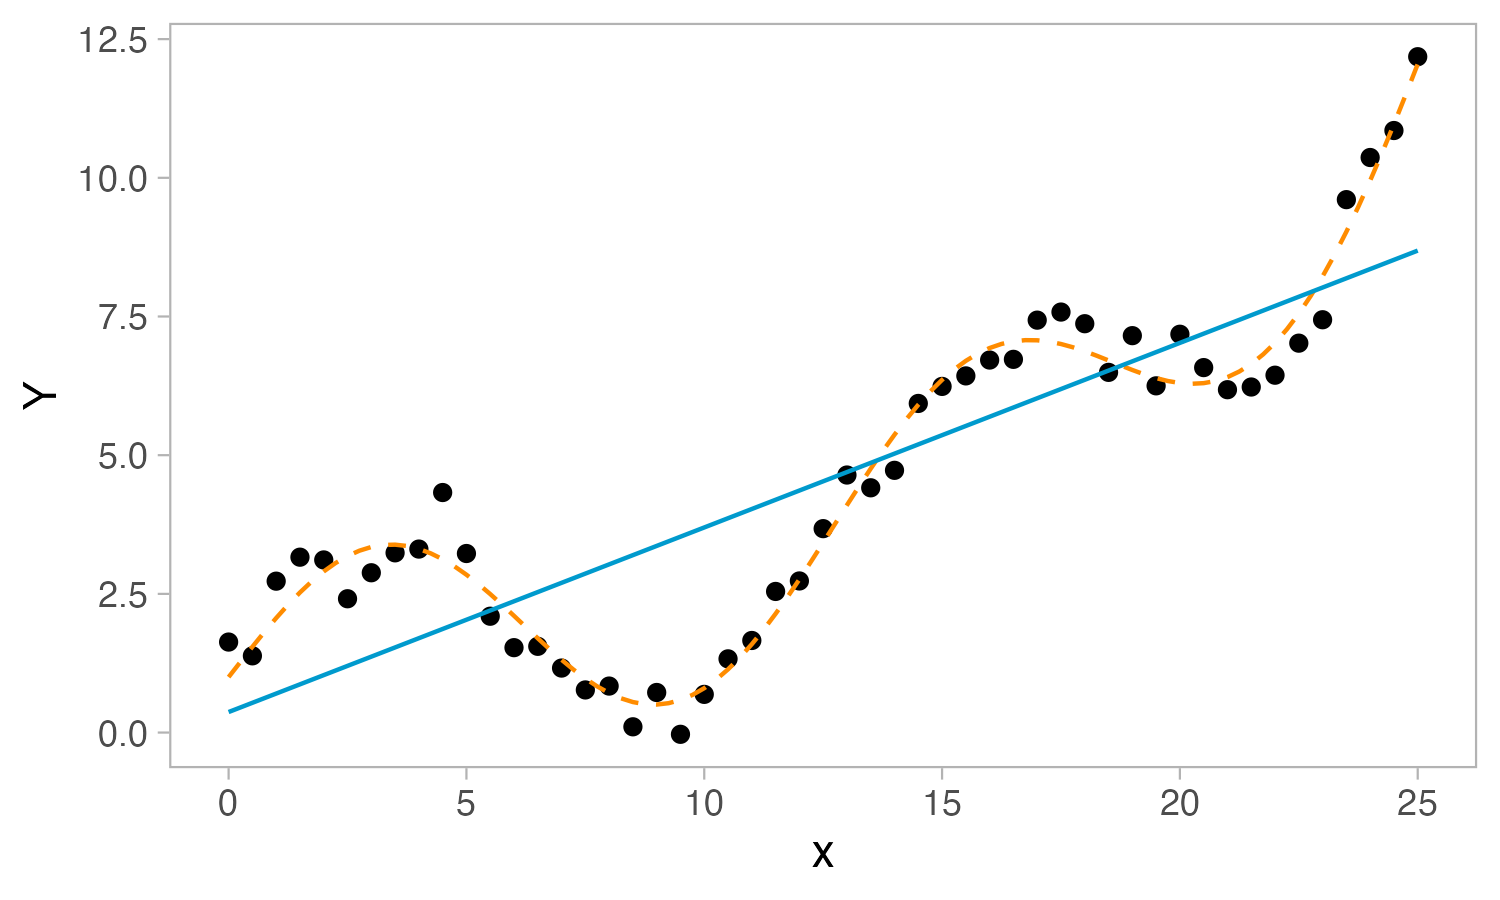
\includegraphics[width=0.75\linewidth]{figures/ch3_toy1} 

}

\caption{Non-linear data with a true relationship (orange) and a fitted linear regression (blue).}\label{fig:toy1}
\end{figure}
Consider the following case where we want to model the relationship between a single predictor and a response variable. Suppose the true relationship between \(x\) and \(Y\) is defined \(Y = e^{\frac{x}{10}} + 2\sin(\frac{x}{2})\). We simulate 51 equally spaced observations of \(x\) from 0 to 25, with error \(\varepsilon_i \overset{\text{iid}}\sim N(0, 0.25)\).

Figure \ref{fig:toy1} illustrates the shape of our simulated non-linear data and the fit proposed by a simple linear regression. We can observe that the linear regression fails to capture the true non-linear relationship. In this case, this would lead to an underestimation of the true association between \(x\) and \(Y\). Now, we will try to capture this relationship using kernel machine regression.
\begin{figure}

{\centering 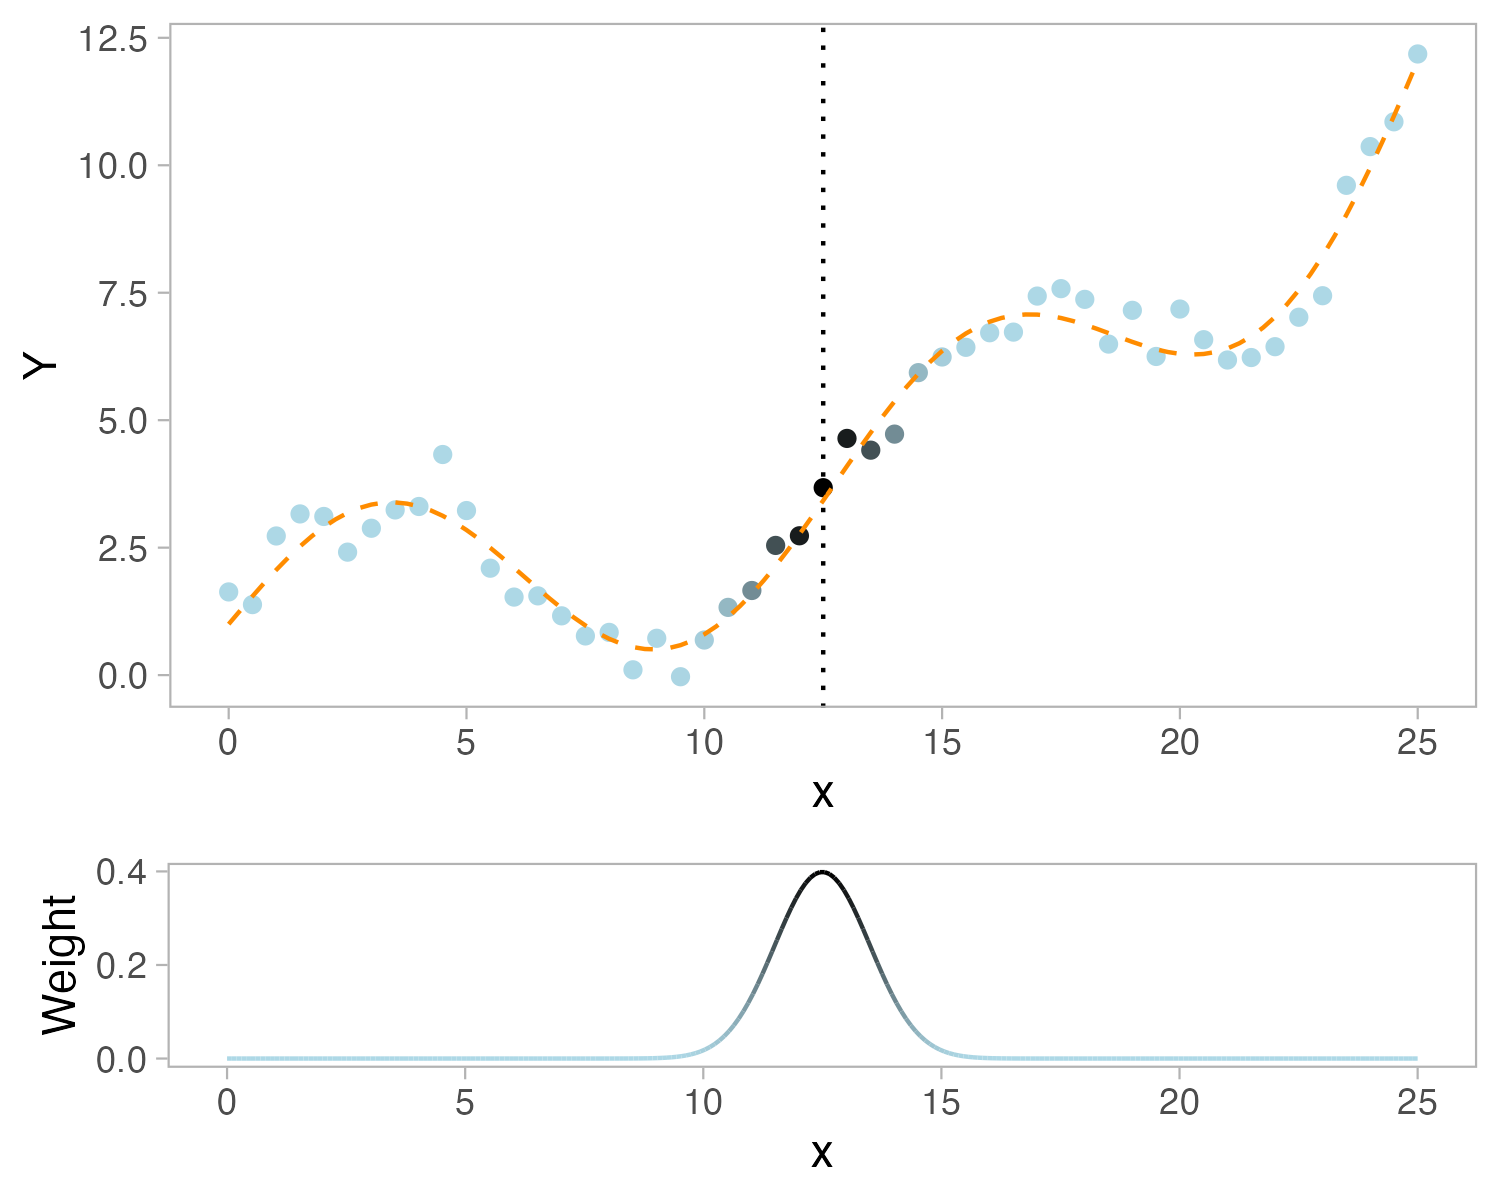
\includegraphics[width=0.75\linewidth]{figures/ch3_toy2} 

}

\caption{A query point of 12.5 and the weights of neighboring observations based on a Gaussian kernel}\label{fig:toy2}
\end{figure}
To visualize how kernel machine regression works as a moving weighted average, we can consider a query point of 12.5. Figure \ref{fig:toy2} identifies the query point and assigns corresponding weights to the neighboring points based on a normal distribution, which shares the same density as the Gaussian kernel. In this case, we will specify \(\rho = 2\), which is synonymous with assigning the weights using a normal distribution with \(\sigma^2=1\). We can see how an appropriate estimate for \(h(12.5)\) can be obtained by taking a weighted average of the \(Y\)'s, with those observations nearby weighted the most heavily.
\begin{figure}

{\centering 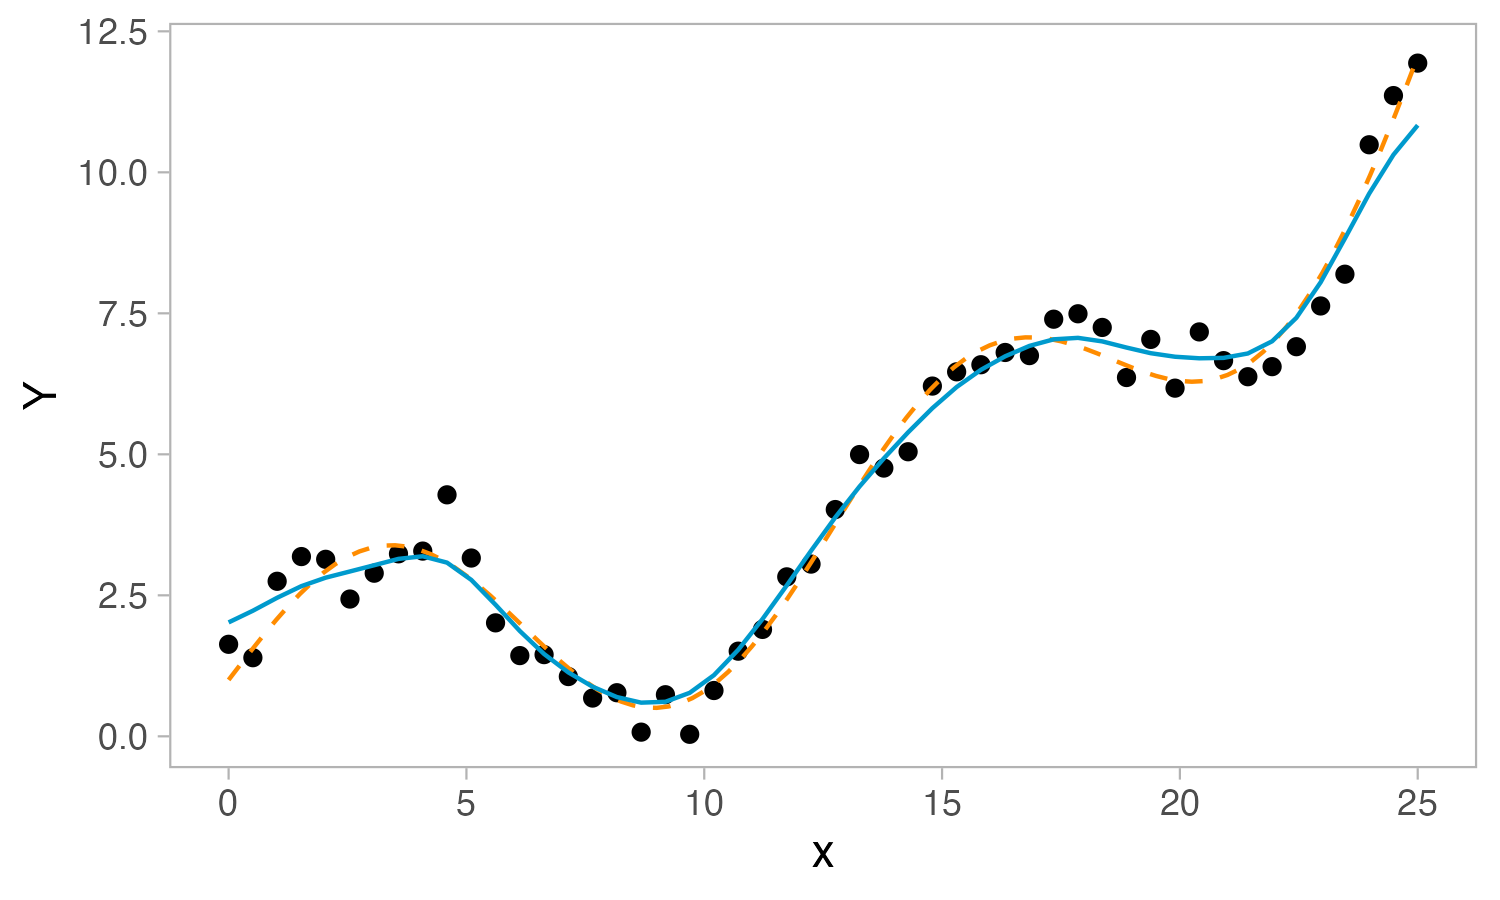
\includegraphics[width=0.75\linewidth]{figures/ch3_toy3} 

}

\caption{Fitted kernel machine regression (blue) with $\rho=2$ compared to the true relationship (orange).}\label{fig:toy3}
\end{figure}
Now, we fit a kernel machine regression on this data with \(\rho=2\) using the \texttt{stats} package in R. We can see in Figure \ref{fig:toy3} that kernel machine regression captures the complex non-linear relationship between \(Y\) and \(x\) and closely follows the true relationship. We do note, though, that the estimation is less precise at the tails, where there is less information provided by local observations. We can also use this example to consider the effect of various values of \(\rho\) on the smoothness of the \(h\) function.
\begin{figure}

{\centering 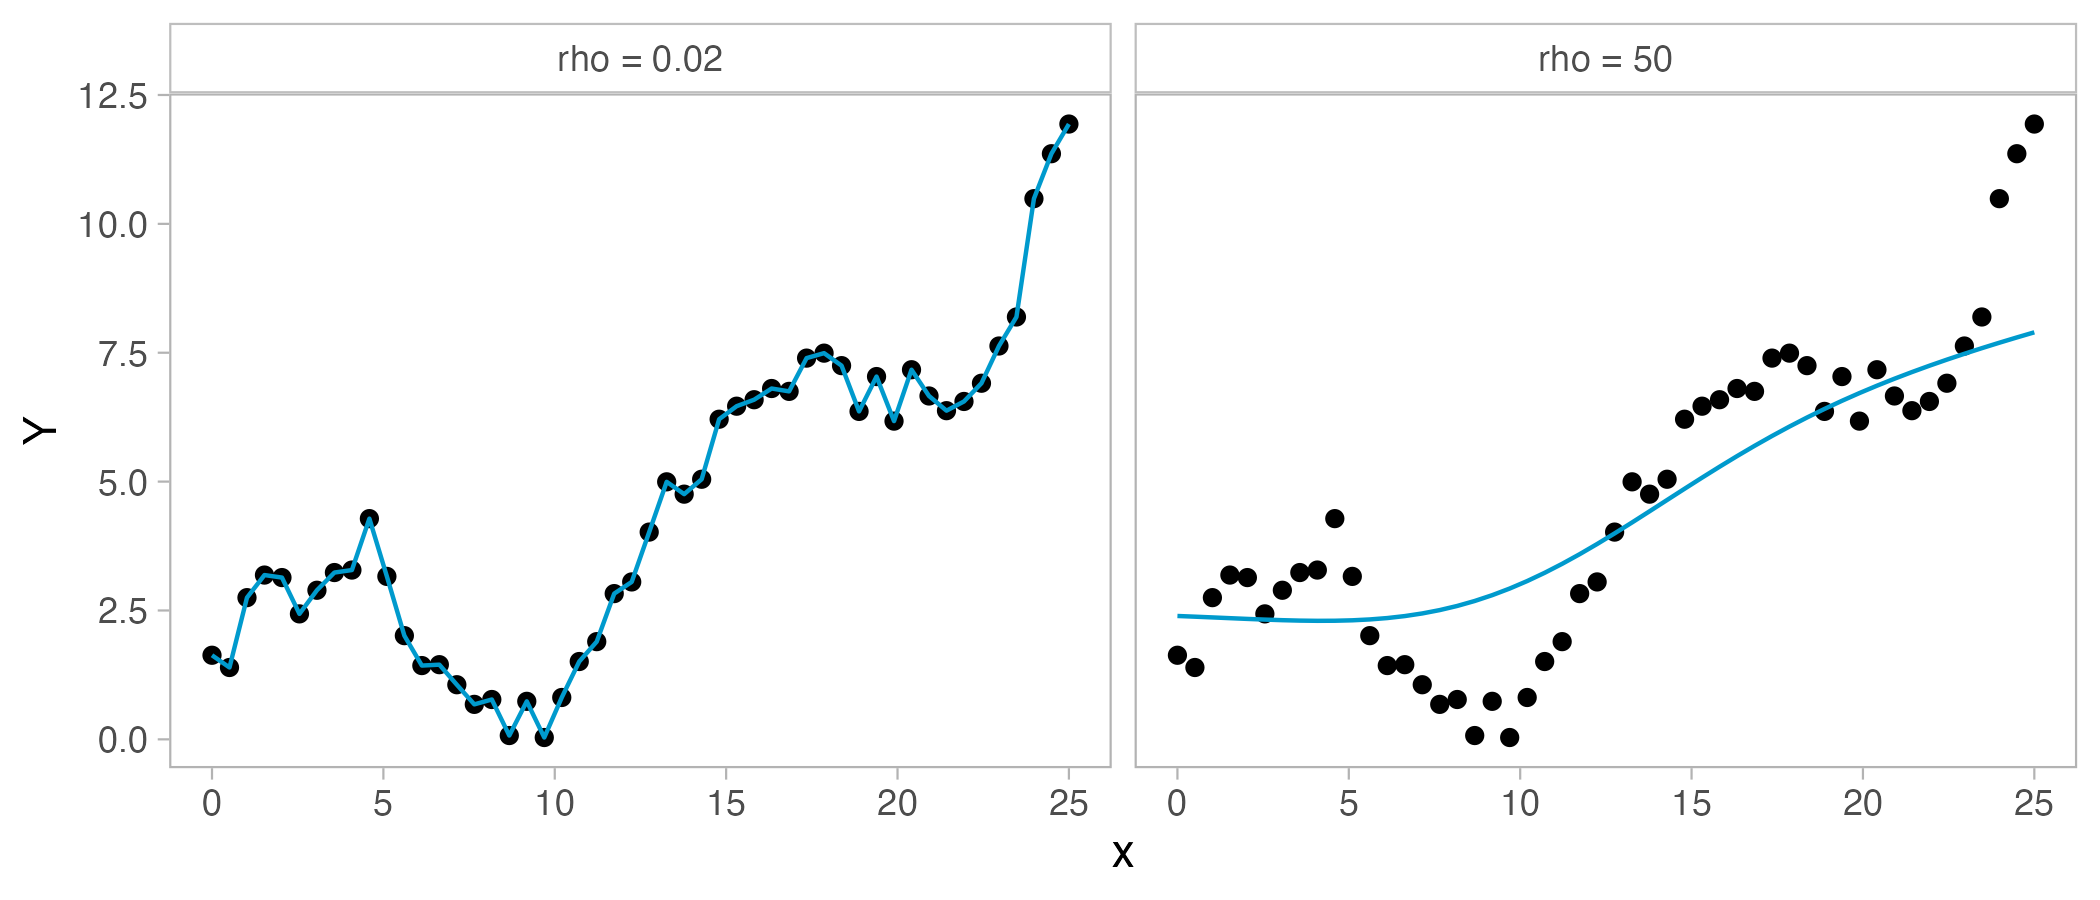
\includegraphics[width=1\linewidth]{figures/ch3_toyrho} 

}

\caption{Fitted kernel machine regression with $\rho=0.02$ (undersmoothed) and $\rho=50$ (oversmoothed).}\label{fig:toyrho}
\end{figure}
Figure \ref{fig:toyrho} demonstrates the effect of relatively smaller and larger values of \(\rho\) on \(h\). Decreasing the value of \(\rho\) allows kernel machine regression to overfit to the noise in the data by relaxing the dependence of neighboring values of \(h\) to each other. On the other hand, increasing the value of \(\rho\) enforces more dependence in \(h\) and as such results in an underfit estimation. Hence, the choice of \(\rho\) has a strong effect on the performance of kernel machine regression.

\hypertarget{variable-selection}{%
\subsection{Variable selection}\label{variable-selection}}

Now that we have defined kernel machine regression, we can extend it to the Bayesian paradigm. Bobb et al. (\protect\hyperlink{ref-bobb_bayesian_2015}{2015}) showed that the Bayesian approach can outperform frequentist kernel machine regression because simultaneous variable selection and estimation can better capture the exposure-response relationship. In this section, we discuss the two methods for Bayesian variable selection in BKMR: hierarchical variable selection and component-wise variable selection (\protect\hyperlink{ref-bobb_bayesian_2015}{Bobb et al., 2015}).

In order to perform variable selection, we define a parameter that puts a weight on each exposure. Each weight controls the degree to which its associated exposure contributes to the model. In component-wise selection, we do this by augmenting the kernel function as

\[
k(\textbf{x}, \textbf{x}'|\textbf{r}) = \text{exp}\bigg\{ -\sum_{m=1}^Mr_m(x_m-x_m')^2 \bigg\},
\]

\noindent where \(\textbf{r}=[r_1,\dots,r_M]^\top\). We define \(r_m=1/{\rho_m}\), the inverse of the tuning parameter \(\rho_m\) for each \(\textbf{x}_m\). Now, we can imagine that an exposure that is not closely associated with the response will be be assigned a value of \(r_m\) close to 0, which corresponds to a larger value of \(\rho_m\). This larger value of \(\rho_m\) means that this exposure would contribute less to the exposure-response relationship, as depicted in the second panel of Figure \ref{fig:toyrho}.

We now define the kernel matrix \(\textbf{K}_{\textbf{X},\textbf{r}}\) as the \(n\times n\) matrix with \((i,j)\)th element \(k(\textbf{x}, \textbf{x}'|\textbf{r})\). To allow \(r_m\) to equal 0 with non-zero probability, we first define an indicator variable determining whether or not a predictor is included in the variable, which is denoted and distributed as

\[
\delta_m \sim \text{Bernoulli}(\pi),
\]

\noindent where \(\pi\) is the prior probability of inclusion. Now, we can assume a ``slab-and-spike'' prior on \(r_m\), distributed as

\[
r_m|\delta_m \sim \delta_mf(r_m) + (1-\delta_m)P_0, 
\]

\noindent where \(f(\cdot)\) is some pdf with support \(\mathbb{R}^+\), and \(P_0\) denotes the density with point mass at 0.

While this process of component-wise variable selection works well in a typical multiple regression setting, it can lead to unreliable estimates in situations where the exposures are highly correlated with each other, which is common in exposure mixture studies. In this case, the correlated components contribute similar information to the model, and component-wise variable selection is not able to distinguish which exposure is important. BKMR deals with this problem by introducing hierarchical variable selection (\protect\hyperlink{ref-bobb_bayesian_2015}{Bobb et al., 2015}).

Hierarchical variable selection involves partitioning the predictors \(\textbf{x}_1, \dots, \textbf{x}_M\) into \(G\) groups, denoted \(\mathcal{S}_g\) with \(g = 1,\dots,G\). These groups should be selected by the user based on prior knowledge, with the aim of keeping within-group correlation high and between-group correlation low (\protect\hyperlink{ref-bobb_bayesian_2015}{Bobb et al., 2015}). For instance, consider a situation with 4 chemicals, Hg, Pb, As, and Sn. If Hg, Pb, and As were strongly correlated with each other and each weakly correlated with Sn, we might define \(\mathcal{S}_1=\{\textrm{Hg, Pb, As}\}\) and \(\mathcal{S}_1=\{\textrm{Sn}\}\).

The indicators from \(r_m|\delta_m\) are now distributed as
\begin{gather*}
\boldsymbol\delta_{\mathcal{S}_g} | \omega_g \sim 
\text{Multinomial}(\omega_g, \boldsymbol\pi_{\mathcal{S}_g}), g=1,\dots,G, \text{ and}\\
\omega_g \sim\text{Bernoulli}(\pi),
\end{gather*}
\noindent where \(\boldsymbol\delta_{\mathcal{S}_g}=\{\delta_m|\textbf{x}_m \in{\mathcal{S}_g}\}\) and \(\boldsymbol\pi_{\mathcal{S}_g}\) are vectors of indicator variables and prior probabilities, respectively, of a exposure \(\textbf{x}_m\) in group \(\mathcal{S}_g\) entering the model. By this approach, at most one exposure in each group is allowed to enter the model (\protect\hyperlink{ref-bobb_bayesian_2015}{Bobb et al., 2015}).

While hierarchical variable selection resolves the issue of multicollinearity, it requires specifying subgroups of predictors a priori and assumes that one exposure in each group can capture the information of the rest. Hence, care should be taken to justify the partitioning of exposures when taking this approach (\protect\hyperlink{ref-bobb_bayesian_2015}{Bobb et al., 2015}).

Note also that the posterior means of \(\delta_m\) generated from these variable selection procedures represent the posterior probability of inclusion of \(\textbf{x}_m\). We can interpret these posterior inclusion probabilities (PIPs) as measures of the relative importance of each exposure. These measures can be used to understand the contribution of each exposure to the health outcome of interest in the model (\protect\hyperlink{ref-bobb_bayesian_2015}{Bobb et al., 2015}).

\hypertarget{bkmrprior}{%
\subsection{Prior specification}\label{bkmrprior}}

In this section, we specify the default prior distributions and parameters used by the BKMR algorithm (\protect\hyperlink{ref-bobb_bayesian_2015}{Bobb et al., 2015}).

BKMR, by default, assumes \(\rho_m=1/r_m \sim \text{Unif}(a_r,b_r)\), a flat prior between \(a_r\) and \(b_r\) for which the default values are 0 and 100, respectively (\protect\hyperlink{ref-bobb_introduction_2017}{Bobb, 2017a}). This defines the prior probability of \(\rho\) as equally distributed across any value from 0 to 100. This inverse of this prior corresponds to the slab component of the ``slab-and-spike'' prior, where \(r_m|\delta_m \sim \delta_m\text{Unif}^{-1}(a_r, b_r) + (1-\delta_m)P_0\). As a flat prior, this distribution should be chosen when we have no prior knowledge about the smoothness of the exposure-response function, with hyperparameters \(a_r\) and \(b_r\) selected to represent the range of values we expect \(\rho\) to potentially span.

We have seen that the smoothness of a kernel machine regression responds strongly to different values of \(r_m=1/\rho\), and, accordingly, the model fit of BKMR is sensitive to their prior distribution. In general, the PIPs generated from the variable selection procedure are particularly sensitive to this prior, though their relative importance tends to remain stable (\protect\hyperlink{ref-bobb_statistical_2018}{Bobb, Claus Henn, Valeri, \& Coull, 2018}). As such, the BKMR algorithm also offers the options to define uniform and gamma priors for the \(r_m=1/\rho\).

Moreover, BKMR assumes that the prior probability of including a predictor (\(\delta_m\)) or group of predictors (\(\omega_g\)) in the model is distributed \(\pi \sim \text{Beta}(a_\pi, b_\pi)\). The default hyperparameters are \(a_\pi=b_\pi=1\), which represent a flat, uninformative prior between 0 and 1. When the hierarchical selection approach is applied, equal values for \(\boldsymbol\pi_{\mathcal{S}_g}\), the probabilities of inclusion for each component in group \(\mathcal{S}_g\), are assumed.

Finally, BKMR assumes that the inverse of the variance of the residuals is distributed \(\sigma^{-2} \sim \text{Gamma}(a_\sigma, b_\sigma)\), with default values of \(a_\sigma=b_\sigma=0.001\), and that the vertical scale of \(h\) is parameterized by \(\lambda \equiv \tau\sigma^{-2} \sim \text{Gamma}(a_\lambda, b_\lambda)\), with default values of \(a_\lambda, b_\lambda\) such that the mean and variance of \(\lambda\) are both equal to 10.

\hypertarget{the-mcmc-algorithm}{%
\subsection{The MCMC algorithm}\label{the-mcmc-algorithm}}

Briefly, we discuss the algorithm used to find the solution in the BKMR package (\protect\hyperlink{ref-bobb_bayesian_2015}{Bobb et al., 2015}, \protect\hyperlink{ref-bobb_statistical_2018}{2018}), with commentary on its implications for the model fitting process.

BKMR uses a Markov chain Monte Carlo (MCMC) algorithm with a mix of Gibbs and Metropolis-Hastings samplers to estimate the posterior distributions of the parameters. In particular, a Gibbs step is used to update the distribution of \(\sigma^2\) while a Metropolis-Hastings step is used to update the distribution of \(\lambda\). For component-wise and hierarchical variable selection, \((\textbf{r}, \boldsymbol\delta, \boldsymbol\omega)\) are sampled jointly using a Metropolis-Hastings sampling scheme.

While each distribution generated by the Gibbs step is always accepted, the distributions for \(\lambda\) and \(r_m\) generated by the Metropolis-Hastings steps are accepted based on an acceptance rate (\protect\hyperlink{ref-wagaman_probability_2021}{Wagaman \& Dobrow, 2021}). The standard deviation of the proposal distribution controls the acceptance rate and as such acts as a tuning parameter (\protect\hyperlink{ref-bobb_example_2017}{Bobb, 2017b}). In general, increasing the standard deviation leads to lower acceptance rates. Acceptance rates that are too low lead to slower convergence, but rates that are too high can cause convergence to a non-optimal distribution.

A major computational limitation of BKMR is that at each iteration of the MCMC algorithm, the \(n \times n\) augmented kernel matrix \(\textbf{K}_{\textbf{Z},\textbf{r}}\) must be inverted multiple times. To offset this, BKMR can employ a Gaussian predictive process which involves specifying a set of \(l\) points, or ``knots,'' that are a subset of the predictor space. The vector of predictors can be approximated by projection onto this lower dimensional space, which allows the algorithm to perform inversions on an \(l\times l\) matrix. A general suggestion is to use this approach to speed up the algorithm when \(n\) is large and to specify \(l\approx n/10\) (\protect\hyperlink{ref-bellavia_statistical_2021}{Bellavia, 2021}).

\hypertarget{bsr}{%
\section{Bayesian semiparametric regression (BSR)}\label{bsr}}

In this section, we introduce the theory of BSR. First, we define the notation that we will be using for spline regression (much of it designed to be consistent with our BKMR presentation):
\begin{itemize}
\tightlist
\item
  \(X_m\) is a predictor variable in the predictor matrix \(\textbf{X}\) with \(m=1,\dots,M\), measuring exposure variables or covariates
\item
  \(\textbf{x}_i\) is a vector of values for a single observation in \(\textbf{X}\) with \(i=1,\dots,n\)
\item
  \(\textbf{z}_i\) is a vector of covariates for a single observation in the matrix \(\textbf{Z}\), which contains a set of covariates, with \(i = 1, \dots, n\)
\item
  \(Y_i\) is an observation of \(\textbf{Y}\), measuring the health outcome in this case
\item
  \(f(\cdot)\) relates \(\textbf{x}_i\) to \(Y_i\) by a set of basis functions, \(b_j(X)\)
\item
  \(\beta_j\) is a weight on the \(j\)th basis function
\item
  \(P\) is the order of the basis expansion
\item
  \(K\) is a set of \(\xi_k\), \(k=1,\dots,K\), interior knots defining \(K+1\) disjoint intervals, and
\item
  \(\boldsymbol\varepsilon_i \overset{\textrm{iid}}\sim N(0,\sigma^2)\) are the residuals of the response.
\end{itemize}
And, we define the notation that we will be using specific to BSR:
\begin{itemize}
\tightlist
\item
  \(\widetilde{X}_m\) is a \(d\)-dimensional basis function expansion of \(X_m\)
\item
  \(\widetilde{X}_{m_1m_2}\) is a \(d^2\)-dimensional basis expansion of the interaction between \(X_{m_1}\) and \(X_{m_2}\)
\item
  \(f^{(h)}(\cdot)\), where \(h=1,\dots,H\) are a set of functions that sum up to \(f(\cdot)\)
\item
  \(\boldsymbol\zeta = \{\zeta_{mh}\}\) is an indicator for whether the \(m\)th predictor is included in the \(h\)th function
\item
  \(\boldsymbol\beta_S^{(h)}\) is a vector of all the coefficients on the predictors in function \(h\)
\item
  \(\sigma^2_{\boldsymbol\beta}\) is the prior variance on the coefficients, and
\item
  \(\boldsymbol\Sigma_{\boldsymbol\beta}\) is a diagonal matrix with the variances of the multivariate slab prior, \(\sigma^2\sigma^2_{\boldsymbol\beta}\), on the diagonals.
\end{itemize}
\hypertarget{spline-regression}{%
\subsection{Spline regression}\label{spline-regression}}

We begin by introducing spline regression, with attention to its specific implementation in BSR. Spline regression is a semiparametric regression technique that can be used to capture non-linear effects. In this introduction, we follow the presentation of spline regression provided by Antonelli et al. (\protect\hyperlink{ref-antonelli_estimating_2020}{2020}), with additional details and explanation from Hastie, Tibshirani, \& Friedman (\protect\hyperlink{ref-hastie_elements_2009}{2009}).

BSR uses spline regression to define the regression relationship as

\[
Y_i = f(\textbf{x}_i) + \textbf{z}_i^\top \boldsymbol{\beta}_{\textbf{z}} +\varepsilon_i,
\]

\noindent where \(f\) is defined by a set of basis functions on the exposures, \(\textbf{x}_i\), \(\textbf{z}_i\) and \(\boldsymbol{\beta}_{\textbf{z}}\) are the covariates and their associated weights, and \(\varepsilon_i\) is a random variable from \(\boldsymbol\varepsilon \overset{\mathrm{iid}}{\sim} N(0, \sigma^2)\). BSR uses natural spline bases (\protect\hyperlink{ref-antonelli_estimating_2020}{Antonelli et al., 2020}). In order to understand how these are constructed, we start with a broad definition of basis expansions, before exploring linear, cubic, and then natural spline bases.

We determine the basis expansion by considering a piece-wise function of \(X_m\) with some order \(P\) and some set of \(K\) knots defining \(K+1\) disjoint intervals. BSR places knots at uniformly sized quantiles within the boundaries of \(X_m\). The most commonly used orders are \(P=1,2,\textrm{and } 4\), the constant, linear, and cubic splines, respectively. To begin, let us consider a continuous piece-wise linear spline basis (i.e., \(P=2\)) of a one-dimensional \(X\) with two interior knots. In this case, we use the following four basis functions:

\nointerlineskip

\[
b_1(X)=1, \hspace{0.25in} b_2(X)=X, \hspace{0.25in} b_3(X)=(X-\xi_1)_+, \hspace{0.25in} b_4(X)=(X-\xi_2)_+,
\]

\noindent where \(\xi_1\) and \(\xi_2\) are the two interior knots, and \(t_+\) denotes the positive part. These bases are used to construct the regression model \(f(X)=\sum_{j=1}^4\beta_jb_j(X)\), which requires estimating \(K+P=4\) parameters. We can check the continuity restrictions at the knots by seeing that \(f(\xi_1^-)=\beta_1 + \xi_1\beta_2\) and \(f(\xi_1^+)= \beta_1 + \xi_1\beta_2+ (\xi_1-\xi_1)\beta_3\) are equal, and likewise at the second knot (\protect\hyperlink{ref-hastie_elements_2009}{Hastie et al., 2009}).

Now, in the case of exposure mixtures, we want smoother functions that can capture the non-linear relationship between the response and the predictors. We can achieve this by increasing the order to \(P=4\) and using a cubic spline, with continuous first and second derivatives at the knots. The cubic spline is the lowest-order spline for which knot-discontinuity cannot be detected by the human eye. For example, for one \(X\) with two interior knots, we use the following six basis functions:
\begin{gather*}
b_1(X)=1, \hspace{0.25in}b_2(X)=X, \hspace{0.25in}b_3(X)=X^2, \\
b_4(X)=X^3, \hspace{0.25in} b_5(X)=(X-\xi_1)^3_+, \hspace{0.25in} b_6(X)=(X-\xi_2)^3_+.
\end{gather*}
\noindent Now, the regression model is defined as \(f(X)= \sum_{j=1}^6\beta_jb_j(X)\) and requires estimating \(K+P=6\) parameters. It can be shown that \(f'(\xi_i^-)= f'(\xi_i^+)\) and \(f''(\xi_i^-)= f''(\xi_i^+)\), and so forth (\protect\hyperlink{ref-hastie_elements_2009}{Hastie et al., 2009}).

However, the behavior of polynomials near the boundaries of \(X\), where there is less information, can be erratic. Natural cubic splines, also referred to as just natural splines, address this by imposing an additional restriction of linearity at the boundaries of \(X\). Paradoxically, this also leads to a simpler model with four fewer parameters to estimate. A general definition of the \(K\) basis functions for a natural spline with interior knots \(\xi_j\), \(j=1,\dots,K\), is given by:
\begin{gather*}
b_1(X)=1, \hspace{0.25in} b_2(X)=X, \hspace{0.25in} b_{k+2}(X)=d_k(X)-d_{K-1}(X), \\
d_k(X)=\frac{(X-\xi_k)^3_+ - (X-\xi_K)^3_+}{\xi_K-\xi_k}.
\end{gather*}
\noindent Here, the regression model is defined as \(f(X) = \sum_{j=1}^K\beta_jb_j(X)\), with \(K\) parameters (\protect\hyperlink{ref-hastie_elements_2009}{Hastie et al., 2009}). BSR uses natural splines to specify the regression relationship.

\hypertarget{toy-example}{%
\subsection{Toy example}\label{toy-example}}

In the following section, we illustrate spline regression using the same toy example used to introduce kernel machine regression. See Chapter \ref{bkmrtoy} and Figure \ref{fig:toy1} for details on the parameters used to generate simulated data.

As in Chapter \ref{bkmrtoy}, we consider a case where we want to model the relationship between a single exposure and a response variable, where the true relationship between \(x\) and \(Y\) is defined as \(Y = e^{\frac{x}{10}} + 2\sin(\frac{x}{2})\). We fit a series of linear, cubic, and then natural spline regressions to illustrate the general framework of a natural spline regression.
\begin{figure}

{\centering 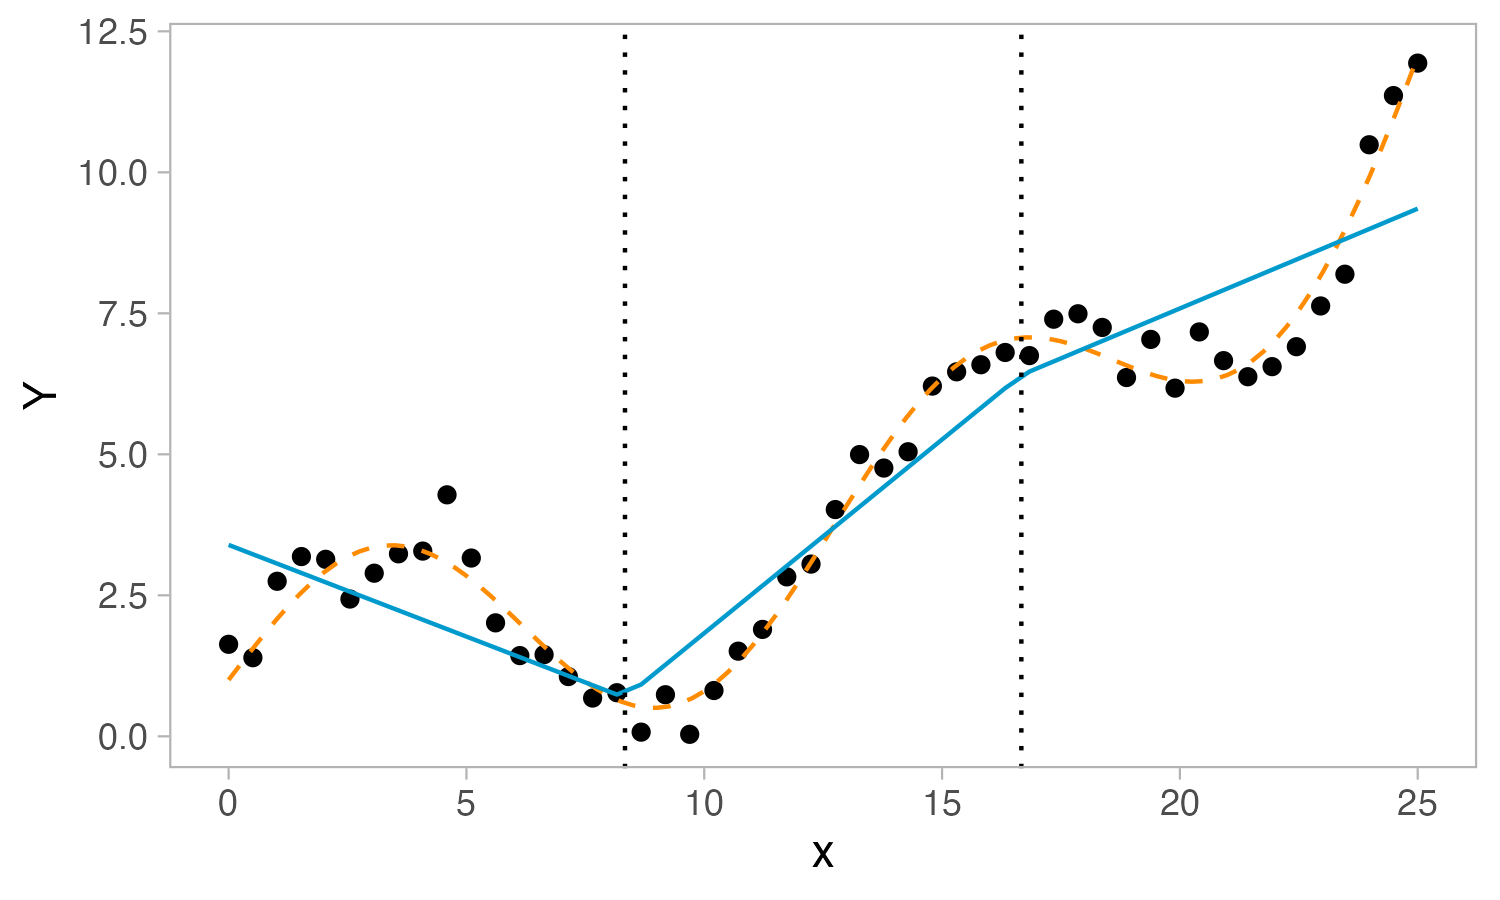
\includegraphics[width=0.75\linewidth]{figures/ch3_toy4} 

}

\caption{Linear spline regression (blue) with four knots (dotted lines) compared to the true relationship (orange).}\label{fig:toy4}
\end{figure}
Figure \ref{fig:toy4} illustrates the fit proposed by a linear spline regression with order \(P=2\). We can see that the implementation of knots allows for even a linear fit to capture more of the nuances in this nonlinear relationship, as compared to a standard linear regression.
\begin{figure}

{\centering 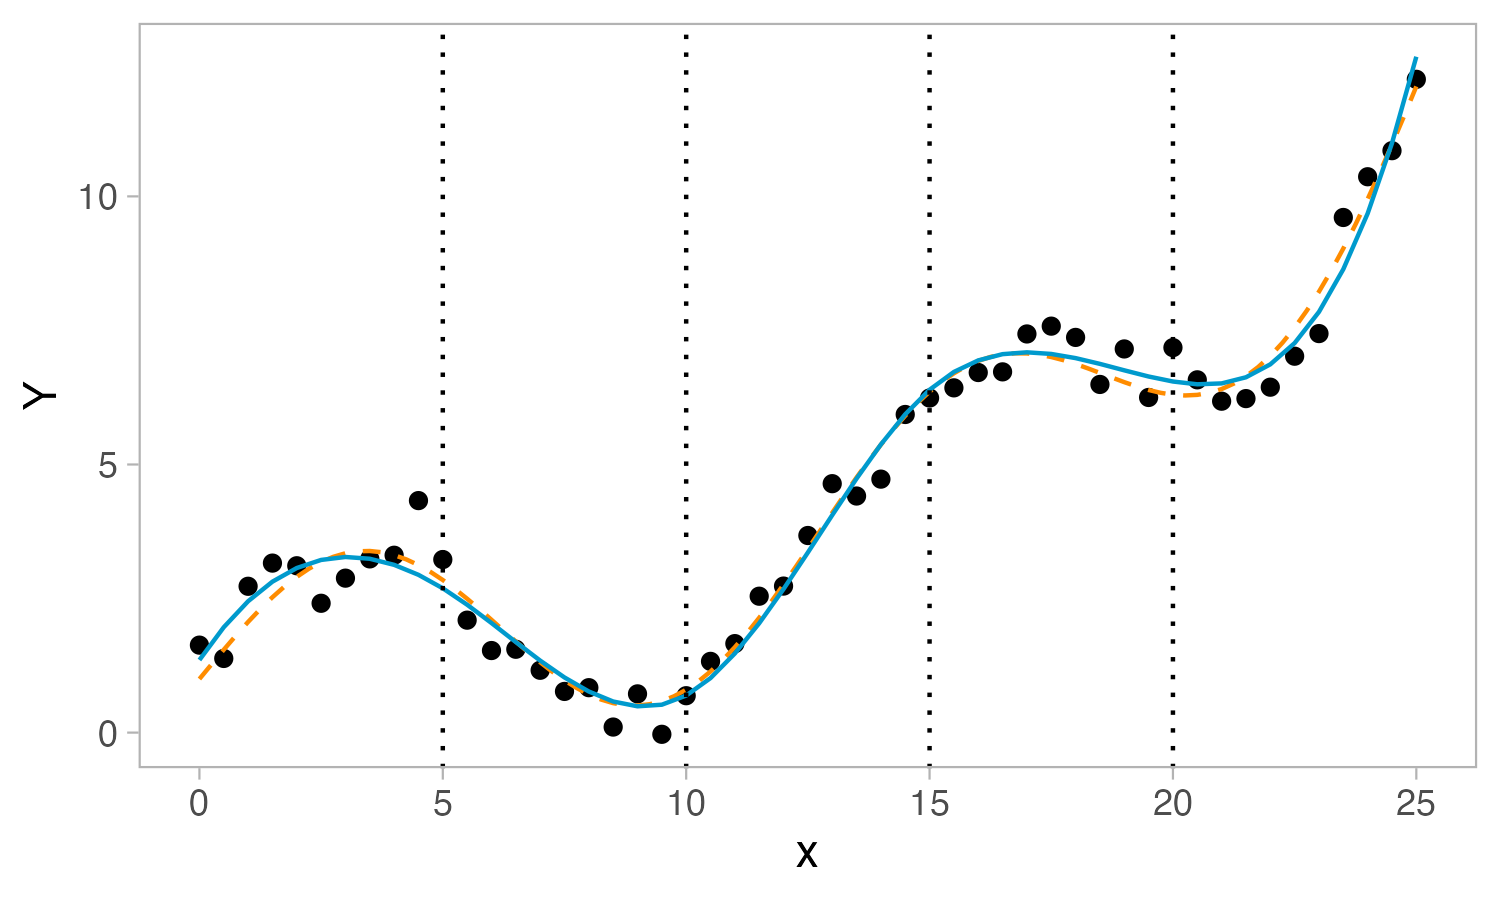
\includegraphics[width=0.75\linewidth]{figures/ch3_toy5} 

}

\caption{Cubic spline regression (blue) with four knots (dotted lines) compared to the true relationship (orange).}\label{fig:toy5}
\end{figure}
\begin{figure}

{\centering 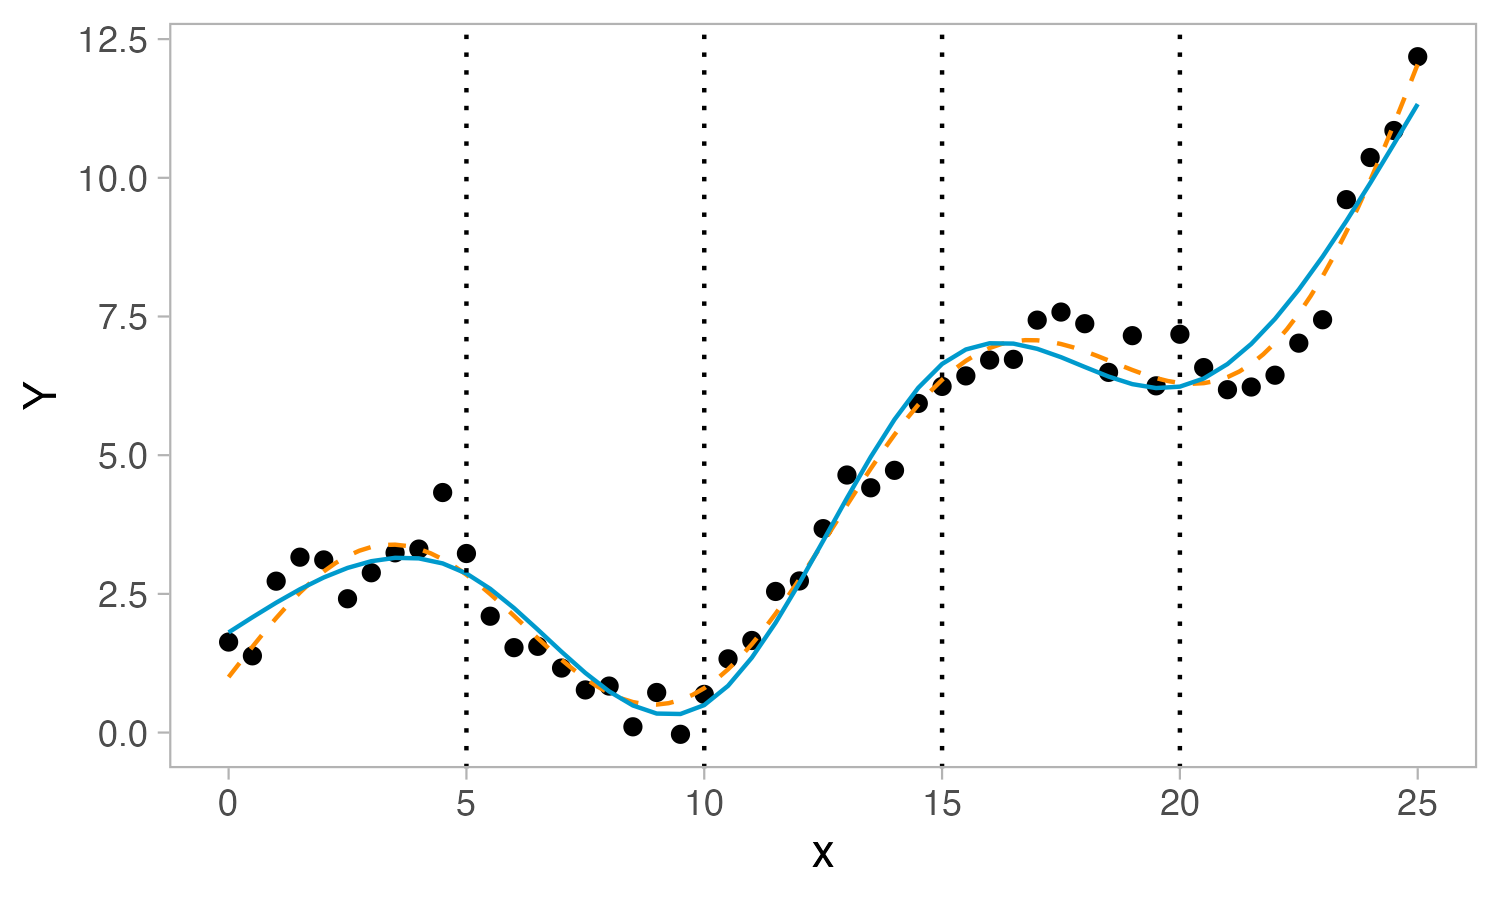
\includegraphics[width=0.75\linewidth]{figures/ch3_toy6} 

}

\caption{Natural spline regression (blue) with four knots (dotted lines) compared to the true relationship (orange).}\label{fig:toy6}
\end{figure}
However, this linear spline regression is still unable to fully estimate the nonlinearity in our example. Increasing the order to \(P=4\) with a cubic spline regression offers additional flexibility. Figure \ref{fig:toy5} illustrates the fit proposed by this model. Here, we can see the benefits of using a cubic polynomial relationship in a nonlinear setting: the estimated relationship is continuous at the knots, and the nonlinear relationship has been flexibly captured.

Our final modification involves imposing linearity constraints on the boundaries of \(x\) to implement a natural spline regression. Figure \ref{fig:toy6} shows the fit estimated using a natural spline regression. The fitted line is only slightly different than that proposed by a cubic spline regression in Figure \ref{fig:toy5}. The most noticeable difference is that the slopes of the tails of the natural spline regression are less extreme than for the cubic spline regression.
\begin{figure}

{\centering 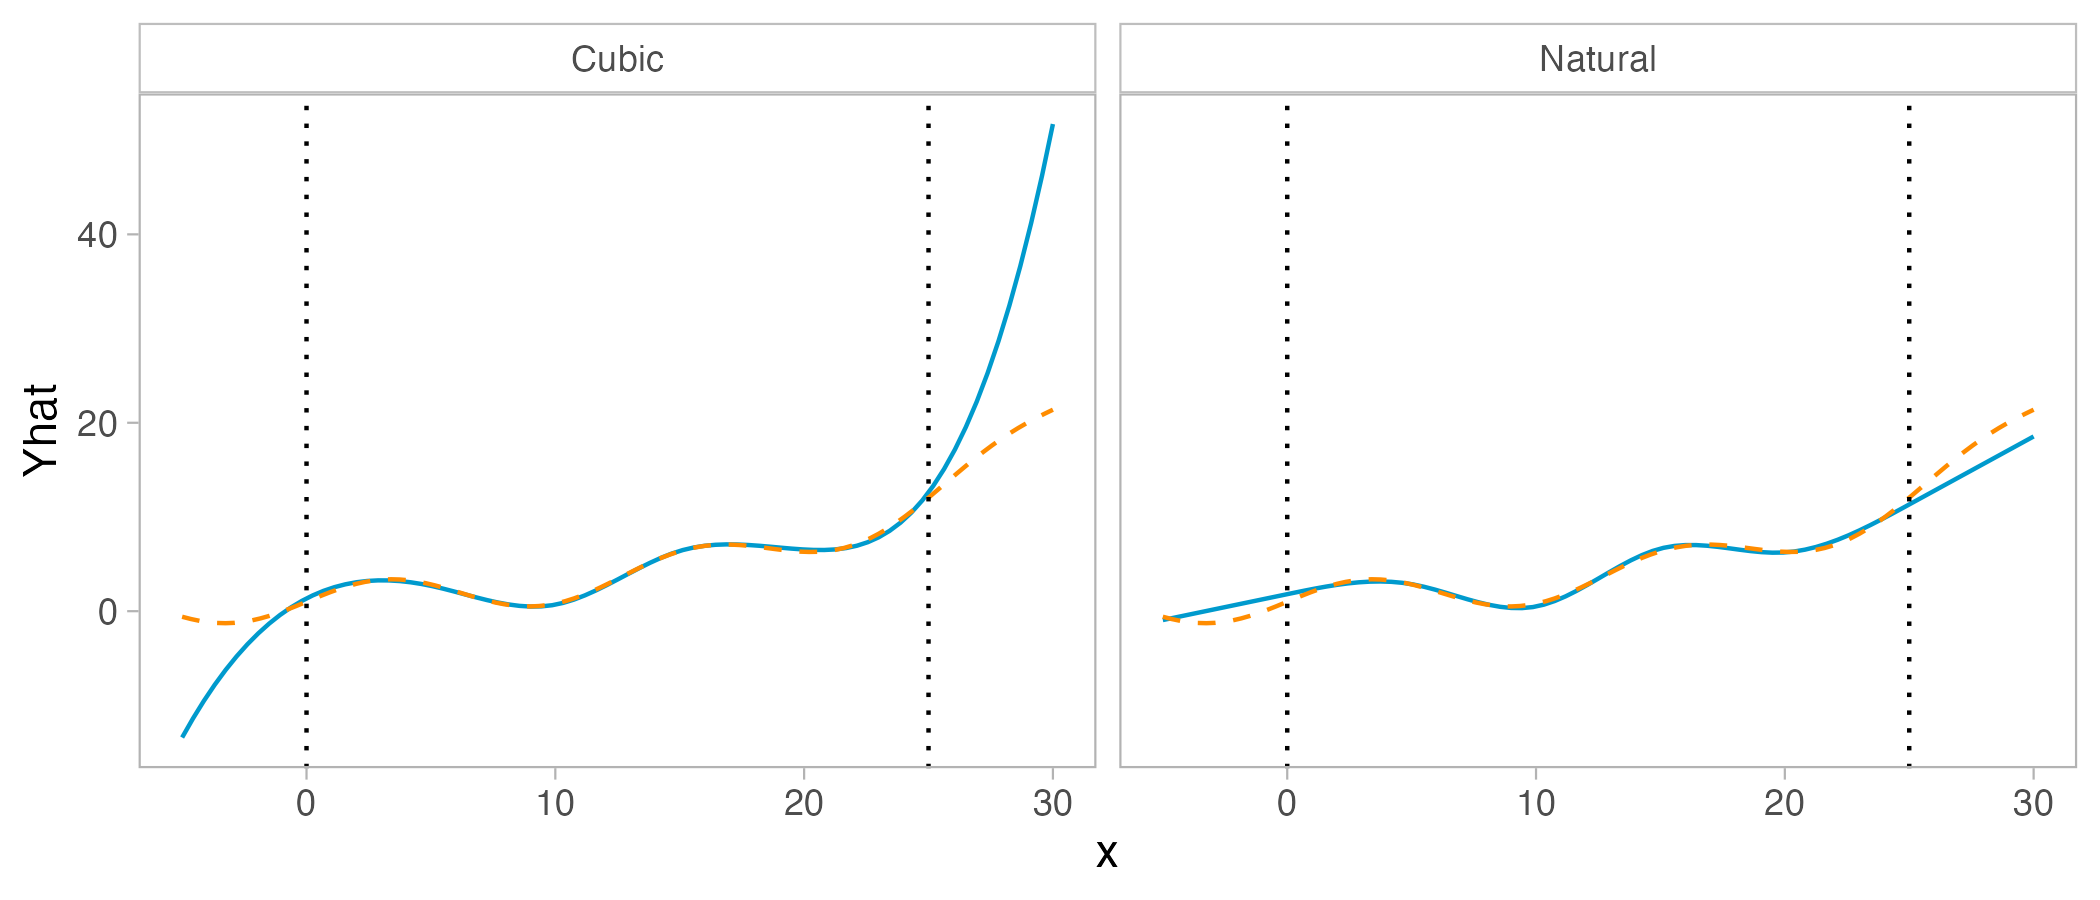
\includegraphics[width=1\linewidth]{figures/ch3_toybounds} 

}

\caption{Natural and cubic spline regression (blue) compared to the true relationship (orange) extrapolated outside the bounds of $x$ (dotted lines).}\label{fig:toybounds}
\end{figure}
Extrapolation outside the scope of \(x\) allows us to see the effect of the linearity constraints imposed by natural regression. Figure \ref{fig:toybounds} demonstrates how the cubic spline regression behaves erratically outside the bounds of \(x\), as the cubic polynomial lines tend toward \(\pm\infty\), while the natural spline regression follows a more appropriate linear trend. As the natural spline regression is more reliable near the boundaries of \(x\) and also simpler to estimate, BSR adopts the use of natural splines.

\hypertarget{model-formulation-in-bsr}{%
\subsection{Model formulation in BSR}\label{model-formulation-in-bsr}}

Now that we have defined natural splines, we introduce BSR, following the presentation in Antonelli et al. (\protect\hyperlink{ref-antonelli_estimating_2020}{2020}). We demonstrate the construction of \(f\) in BSR by first assuming a two-dimensional case with exposures \(X_1\) and \(X_2\). We define
\begin{gather*}
f(X_1) = \widetilde{X}_1\boldsymbol{\beta}_1, \hspace{0.25in} f(X_2) = \widetilde{X}_2\boldsymbol{\beta}_2,\\
f(X_1,X_2) = \widetilde{X}_1\boldsymbol{\beta}_1 + \widetilde{X}_2\boldsymbol{\beta}_2 + \widetilde{X}_{12}\boldsymbol{\beta}_{12},
\end{gather*}
\noindent where \(\widetilde{X}_m=[b_{m1}(X_m),\dots,b_{md}(X_m)]\) represents a \(d\)-dimensional basis function expansion for \(m=1,2\), and \(\widetilde{X}_{12}= [b_{11}(X_1)b_{21}(X_2), b_{11}(X_1)b_{22}(X_2), \dots, b_{1d}(X_1)b_{2d}(X_2)]\) represents a \(d^2\)-dimensional basis expansion of the interaction between \(X_1\) and \(X_2\). \(d\) is an influential tuning parameter. BSR by default assumes that all exposures have the same number of degrees of freedom and uses the Watanabe-Akaike (WAIC) model selection criterion to select \(d\), which approximates leave one out cross validation. Note that we must explicitly model the effect of the interaction term by assuming a multiplicative interaction between the basis functions of the predictors.

Extending to the multi-dimensional setting, BSR assumes the following general model formulation:
\begin{gather*}
f(\textbf{x}_i)= \sum_{h=1}^Hf^{(h)}(\textbf{x}_i), \\
f^{(h)}(\textbf{x}_i)= \sum_{m_1=1}^M\widetilde{x}_{im_1}\boldsymbol\beta_{m_1}^{(h)} + 
\sum_{m_1=2}^M\sum_{m_2<m_1}\widetilde{x}_{im_1m_2}\boldsymbol\beta_{m_1m_2}^{(h)} + \dots,
\end{gather*}
\noindent where \(f^{(h)}(\textbf{x}_i)\) includes a summation of all \(M\)-way interactions. The inclusion of all \(M\)-way interactions makes the model far too overparameterized. Moreover, \(f(\textbf{x}_i)\) is a sum of \(k\) different functions \(f^{(h)}(\textbf{x}_i)\) where a value for \(H\) is selected in order to capture all exposure effects in the model. Each of the \(H\) functions has the same functional form, and so the regression coefficients for a function \(f^{(h)}(\textbf{x}_i)\) are only identifiable up to a constant --- this means that there are multiple sets of coefficients that could be estimated from the same data.

\hypertarget{sparsity-inducing-priors}{%
\subsection{Sparsity inducing priors}\label{sparsity-inducing-priors}}

In order to handle the overparameterization and non-identifiability of the model, BSR implements multivariate sparsity inducing priors. In this section, we follow the presentation provided in Antonelli et al. (\protect\hyperlink{ref-antonelli_estimating_2020}{2020}).

First, we define indicators \(\boldsymbol\zeta=\{\zeta_{mh}\}\) representing whether the \(m\)th exposure is included in the \(h\)th function:
\begin{align*}
P(\zeta_{mh}=1) &= \tau_h^{\zeta_{mh}}(1-\tau_h)^{1-\zeta_{mh}} 
I(A_h\not\subset A_{h'}\forall h'\neq h \textrm{ or } A_h=\{\}),\\
&\textrm{where } A_h=\{m:\zeta_h=1\}.
\end{align*}
\noindent Here, the indicators follow a Bernoulli distribution with prior probability of inclusion \(\tau_h\). The posterior means of \(\boldsymbol\zeta\), i.e.~the PIPs, can be interpreted as measures of relative variable importance. We include an indicator function \(I()\) that represents whether the function \(h\) contains a unique set of predictors. This indicator ensures that no function contains exposures that are a subset of those in another function, \(h'\), in which case this function would be redundant and thus removed from the model entirely.

Now, we assume a multivariate slab-and-spike prior on the regression coefficients:
\begin{align*}
P(\boldsymbol\beta_S^{(h)}|\boldsymbol\zeta) &= \bigg(1-\prod_{m\in S}\zeta_{mh}\bigg)P_{\textbf{0}} +
\bigg(\prod_{m\in S}\zeta_{mh}\bigg) \psi_1(\boldsymbol\beta_S^{(h)}), \\
&\textrm{where } S \textrm{ is some subset of } {1, 2, \dots, m}.
\end{align*}
\noindent Here, \(P_{\textbf{0}}\) denotes the density with point mass at \(\textbf0\), and \(\psi_1()\) is a multivariate normal distribution with mean \(\textbf0\) and covariance \(\boldsymbol\Sigma_{\boldsymbol\beta}\), a diagonal matrix with \(\sigma^2\sigma_{\boldsymbol\beta}^2\) on the diagonals.

\hypertarget{bsrprior}{%
\subsection{Prior specification}\label{bsrprior}}

In this section, we discuss the priors and their default specifications in BSR (\protect\hyperlink{ref-antonelli_estimating_2020}{Antonelli et al., 2020}).

The priors on \(\boldsymbol\Sigma_{\boldsymbol\beta}\), the diagonal matrix with \(\sigma^2\sigma^2_{\boldsymbol\beta}\) on the diagonals, control the shrinkage of \(\boldsymbol\beta_S^{(h)}\). Variable selection is sensitive to the choice of prior on this parameter, so BSR implements an empirical Bayes strategy to obtain a prior distribution for \(\sigma^2_{\boldsymbol\beta}\) based on the data. While this is not a fully Bayesian approach, it has been shown that this strategy works better in practice (\protect\hyperlink{ref-antonelli_estimating_2020}{Antonelli et al., 2020}). Additionally, the default prior for \(\sigma^2\) is assumed to follow a \(\textrm{Gamma}(0.001, 0.001)\) distribution.

However, when there is a weak relationship between the exposures and relationship, the estimated prior variance for the slab \(\sigma^2_{\boldsymbol\beta}\) can be very small. In this case, the shape of the slab approximates the point mass of 0 at the spike, and the PIPs become difficult to accurately estimate. BSR avoids this by imposing a lower bound on the variance. This is determined by establishing a constant value for \(\tau_h\), the prior probability of inclusion, for all \(h\) and then permuting the rows of \(Y\) (i.e., breaking up the relationship). Then, a grid of values for \(\sigma^2_{\boldsymbol\beta}\) are tested until some predefined threshold of the posterior probability of inclusion is obtained (e.g., 0.25 for a main effect and 0.05 for a two-way interaction). If the empirical Bayes estimate for \(\sigma^2_{\boldsymbol\beta}\) is less than this lower bound, then the lower bound is used instead.

Finally, BSR assumes that \(\tau_h \sim \textrm{Beta}(L,\gamma)\), which defines the prior probability of including a predictor for all functions \(h\). If \(L\) is some predefined constant, and \(\gamma=m\), the number of predictors, then the prior amount of sparsity should increase as the number of predictors increases (\protect\hyperlink{ref-antonelli_estimating_2020}{Antonelli et al., 2020}).

\hypertarget{the-mcmc-algorithm-1}{%
\subsection{The MCMC algorithm}\label{the-mcmc-algorithm-1}}

We also briefly discuss the MCMC algorithm employed by BSR (\protect\hyperlink{ref-antonelli_estimating_2020}{Antonelli et al., 2020}).

BSR uses an MCMC algorithm to obtain posterior distributions of \(\sigma^2\) and \(\tau_h\). In particular, Gibbs samplers are employed to sample \(\sigma^2\) and \(\tau_h\) from their full distributions and to update \(\boldsymbol\zeta\) and \(\boldsymbol\beta_S^{(h)}\). Every \(T\) MCMC iterations, BSR uses a Monte Carlo expectation maximization algorithm with a Gibbs sampler to update \(\sigma^2_{\boldsymbol\beta}\). The empirical Bayes estimate is obtained once \(\sigma^2_{\boldsymbol\beta}\) converges, at which point the MCMC runs conditional on this estimated variance.

Notably, this algorithm must deal with the explicit specification of interaction terms in the model. Any additive univariate effect or lower-order interaction term is, by definition, a subset of some higher-order interaction term. As the MCMC algorithm searches the model space, it might accept a move to a higher-order interaction and get stuck in a local mode when, in reality, a simpler model should be preferred. BSR handles this challenge by imposing a constraint in the MCMC algorithm: if the inclusion of a \(p\)th order interaction term is being considered, then the algorithm must also evaluate all \((p-1)\)th order models. If the truth is some lower-order model, then this strategy avoids the undesirable convergence to a local mode. When the model is complex, maintaining reversibility of updates under this strategy can be computationally challenging with a Gibbs sampler; in this case, using a Metropolis Hastings sampler is computationally faster (\protect\hyperlink{ref-antonelli_estimating_2020}{Antonelli et al., 2020}).

\hypertarget{detecting-interactions}{%
\section{Detecting interactions}\label{detecting-interactions}}

In Chapter \ref{motivation}, we highlighted the challenges of analytically testing for the presence of interactions in exposure mixture studies. These challenges motivated a theoretical exploration of BKMR and BSR in Sections \ref{bkmr} and \ref{bsr}. Now, we discuss and compare the options that BKMR and BSR provide for inference on the presence of interactions. We also include discussion on theoretical advantages and disadvantages to each. Importantly, we note that it is not possible to detect interactions between a covariate and an exposure within the model specifications of BKMR or BSR.

\hypertarget{bkmr-1}{%
\subsection{BKMR}\label{bkmr-1}}

Since the flexible \(h\) function in kernel machine regression allows us to forgo any assumptions about the nature of the relationship between the health outome and exposures, BKMR can potentially capture complex interactions between exposures The challenge with using BKMR to do this, however, is that there is no formal framework for conducting inference on the presence of interactions.

Currently, the most common approach to detecting interactions is through a qualitative assessment of visual diagnostic plots (\protect\hyperlink{ref-bobb_introduction_2017}{Bobb, 2017a}). Two- or three-way interactions can be assessed by plotting the estimated exposure-response relation for one/two exposures at various quantiles of another exposure, while setting all other exposures at fixed quantile values. For instance, if we are interested in the interaction between \(X_1\) and \(X_2\), we can plot the estimated regression line against \(X_1\) at the 0.25, 0.5, and 0.75 quantiles of \(X_2\) and vice versa. In the three-way case of \(X_1\), \(X_2\), and \(X_3\), we can plot the estimated regression surface against \(X_1\) and \(X_2\) at the 0.25, 0.5, and 0.75 quantiles of \(X_3\). If the shape of the estimation changes meaningfully, then there might be evidence of an interaction.

A slightly more formal inferential approach for two-way interactions involves using summary statistics (\protect\hyperlink{ref-bobb_introduction_2017}{Bobb, 2017a}, \protect\hyperlink{ref-bobb_example_2017}{2017b}). In this case, we can calculate the difference in estimated response values for \(X_1\) at two quantiles, say, 0.25 and 0.75, of \(X_2\) and then generate a confidence interval. If we observe that the interval does not contain 0, then there is evidence of an interaction. The choice of quantiles here is important. If there is a parachute-like regression surface between the response and two exposures, the summary statistics might mask the true nature of the relationship.

Notably, if we specify hierarchical variable selection to handle multicollinearity, then only one exposure in each a priori defined group can enter the model. If there exists some true interaction between exposures in one group, then BKMR will be unable to incorporate it into the final model. Moreover, interactions between exposures in separate groups can only be identified if both are selected into the final model based on their within-group PIPs. Hence, if detecting interactions is a goal when using BKMR with hierarchical variable selection, groups should be carefully selected, and the influence of group membership should be considered in model interpretation.

\hypertarget{bsr-1}{%
\subsection{BSR}\label{bsr-1}}

Providing formal inference on the presence of interactions was one of the primary motivations for the development of BSR. BSR explicitly incorporates interaction terms in its model formulation, and the model fitting process assigns PIPs for any \(m\)-dimensional interaction from the posterior means of the \(\boldsymbol\zeta\) matrix. Such probabilities can be used as a quantifiable measure of the strength of a potential interaction. We can also compare PIPs for interactions with the PIPs for their individual components, which can be used to compare exposures' interactive effects with their marginal effects.

The visualization and summary statistics approaches available in BKMR are also possible in BSR. In particular, it is helpful to follow up the identification of a potential interaction with a visual assessment using the estimated exposure-response relationship at fixed quantiles of other predictors. The major benefit of BSR is that the PIPs serve as a quantifiable uncertainty metric for the presence of interactions.

\hypertarget{differences-between-bkmr-and-bsr}{%
\subsection{Differences between BKMR and BSR}\label{differences-between-bkmr-and-bsr}}

We have explained how the inferential framework of BSR improves upon the BKMR approach for the detection of complex interactions. We also briefly compare general features of their model formulations.

While BKMR is a fully nonparametric approach, BSR is a semiparametric approach because it makes distributional assumptions about the data (i.e., that the relationship can be adequately captured by a \(d\)-dimensional natural spline basis expansion). As BKMR uses the kernel technique, its implementation can become computationally intensive for datasets with large \(n\), as it scales with \(n^2\), while BSR is able to scale with \(n\) (\protect\hyperlink{ref-antonelli_estimating_2020}{Antonelli et al., 2020}).

BSR is highly sensitive to the choice of \(d\), the degrees of freedom. While it employs a WAIC approach to selecting the best \(d\), this parameter introduces an additional tuning step in the analysis. Both approaches can be highly sensitive to the specification of certain priors. BSR offers an empirical Bayes strategy to estimate \(\sigma^2_{\boldsymbol\beta}\), the variance of a exposure's prior probability of inclusion. On the other hand, the choice of prior on the influential smoothing parameter, \(\rho\), in BKMR is up to the user.

We also note that BKMR offers a hierarchical variable selection approach to dealing with collinearity between exposures. While this is an additional decision that must be specified by the user, it offers a formal approach to dealing with collinear exposures. BSR does not explicitly account for collinearity in its model formulation, which can lead to erroneous interpretations of variable importance if unaccounted for.

\hypertarget{sims}{%
\chapter{Simulations}\label{sims}}

\hypertarget{past-simulation-studies}{%
\section{Past simulation studies}\label{past-simulation-studies}}

Here, we preface our simulation study with an overview of examples in the literature which compare various methods for exposure mixture studies using simulations. Taylor et al. (\protect\hyperlink{ref-taylor_statistical_2016}{2016}) conclude that, in general for exposure mixture studies, no single method consistently outperforms others across all situations and, importantly, that a method should be chosen based on the question of interest. Thus, for each study, we highlight not only the findings, but also the data-generating scenarios and the identified question of interest.

Lazarevic et al. (\protect\hyperlink{ref-lazarevic_performance_2020}{2020}) compare the performance of a broad range of methods for accurate variable selection of important exposures. They simulated exposure data using a multivariate copula based on real-world data and the response by specifying a regression model with only a subset of truly significant exposures and a normal error term. Two correlation structures were considered --- one with the original Spearman correlation matrix and one with the values halved --- as well as two signal-to-noise ratios --- one with an \(R^2\) for the true model at 10\% and one at 30\%. They found that BKMR, along with three other flexible regression methods that allow for nonlinearity, provided more accurate variable selection results compared to two machine learning methods. Moreover, they observed that, in general, low signal-to-noise ratios had a stronger impact on performance than did increasing multicollinearity.

Hoskovec et al. (\protect\hyperlink{ref-hoskovec_model_2021}{2021}) compare Bayesian methods, including BKMR, while considering 4 research questions: accurate estimation, selection of important exposures, exclusion of unimportant exposures, and identification of interactions. They use observed exposure and covariate data to simulate response data using regression relationships; they considered three exposure-response scenarios of varying complexity and included two-way multiplicative interaction terms. For each simulated dataset, they randomly assigned exposures to be active components of the mixture to incorporate variability in the data. Overall, they found that Bayesian methods outperformed traditional linear regressions, and that BKMR performed best when the exposure-response function takes on a complex form.

Most recently, Pesenti et al. (\protect\hyperlink{ref-pesenti_comparative_2023}{2023}) compare BKMR, BSR, and the Bayesian Least Absolute Shrinkage and Selection Operator (LASSO) for variable selection. Data were generated using a multivariate normal with moderate and strong correlation structures specified manually by the researchers. They found that, in situations with additive and linear exposure-response relationships, Bayesian LASSO was appropriate. Across the other scenarios, BKMR generally performed best, while BSR selected exposures with high heterogeneity when the sample size was smaller due to the influence of the degrees of freedom, \(d\), tuning parameter. Notably, multicollinearity did not generally lead to spurious variable selection.

Finally, we briefly comment on studies by Sun et al. (\protect\hyperlink{ref-sun_statistical_2013}{2013}) and Barrera-Gómez et al. (\protect\hyperlink{ref-barrera-gomez_systematic_2017}{2017}), whose explicit goal is to compare methods for identifying interactions. Both studies generate exposure data using the correlation structure from an existing dataset; Sun et al. (\protect\hyperlink{ref-sun_statistical_2013}{2013}) uses a multivariate lognormal, while Barrera-Gómez et al. (\protect\hyperlink{ref-barrera-gomez_systematic_2017}{2017}) uses a multivariate normal. Both only consider two-way, multiplicative interactions. While neither of these studies consider the methods used in this thesis, they find that, in general, models that formally allow for interaction effects perform better than models that only allow for univariate additive effects.

\hypertarget{methods}{%
\section{Methods}\label{methods}}

The goal of our simulation study is to provide guidance on the choice between BSR and BKMR for characterizing a diverse range of complex interactions between predictors. In particular, we aim to extend findings from previous simulation studies by considering a more comprehensive range of interaction types, including different effect sizes, non-multiplicative interactions, and three-way interactions. We also explore interactions between exposures and categorical covariates, a previously understudied form of interaction in exposure mixture studies. Hereafter, we refer to exposures and chemicals interchangably.

\hypertarget{madres}{%
\subsection{MADRES data}\label{madres}}

In order to make our simulations comparable to real-world exposure mixture studies, we based our simulation data on the Maternal And Developmental Risks from Environmental and Social Stressors (MADRES) pregnancy cohort. The MADRES cohort is an ongoing, prospective pregnancy cohort of predominantly lower-income, Hispanic women in Los Angeles, California, which began in 2015 (\protect\hyperlink{ref-bastain_study_2019}{Bastain et al., 2019}). Urine samples were collected by participants at their first visit, and questionnaires were administered during their first visit, with follow-ups at the first, second, and third trimesters. See Bastain et al. (\protect\hyperlink{ref-bastain_study_2019}{2019}) for further details on study design.

Howe et al. (\protect\hyperlink{ref-howe_prenatal_2020}{2020}) previously examined the effect of prenatal metal mixtures of birth weight (BW) for gestational age (GA) in this cohort. They used BKMR to identify associations between metal mixtures and BW for GA, as well as BSR to conduct inference on interactions between metals. Using BKMR, they found that, of the metals in the mixture, mercury and nickel were most strongly associated with BW for GA. Moreover, BKMR results suggested that a potential interaction between mercury and nickel exists; however, when run through BSR, the PIP for this interaction was extremely small, despite being the highest of all two-way interactions.

Data from the study by Howe et al. (\protect\hyperlink{ref-howe_prenatal_2020}{2020}) were obtained from publicly available data in the Human Health Exposure Resource (HHEAR) Data Repository, which has been approved under Icahn School of Medicine at Mount Sinai IRB Protocol \#16-00947. The Digital Object Identifiers associated with the urinary trace element data and epidemiological data are 10.36043/1945\_159 and 10.36043/1945\_177, respectively. All analyses were conducted in R v4.3.2 (\protect\hyperlink{ref-r_core_team_r_2013}{R Core Team, 2013}).
\begin{figure}

{\centering 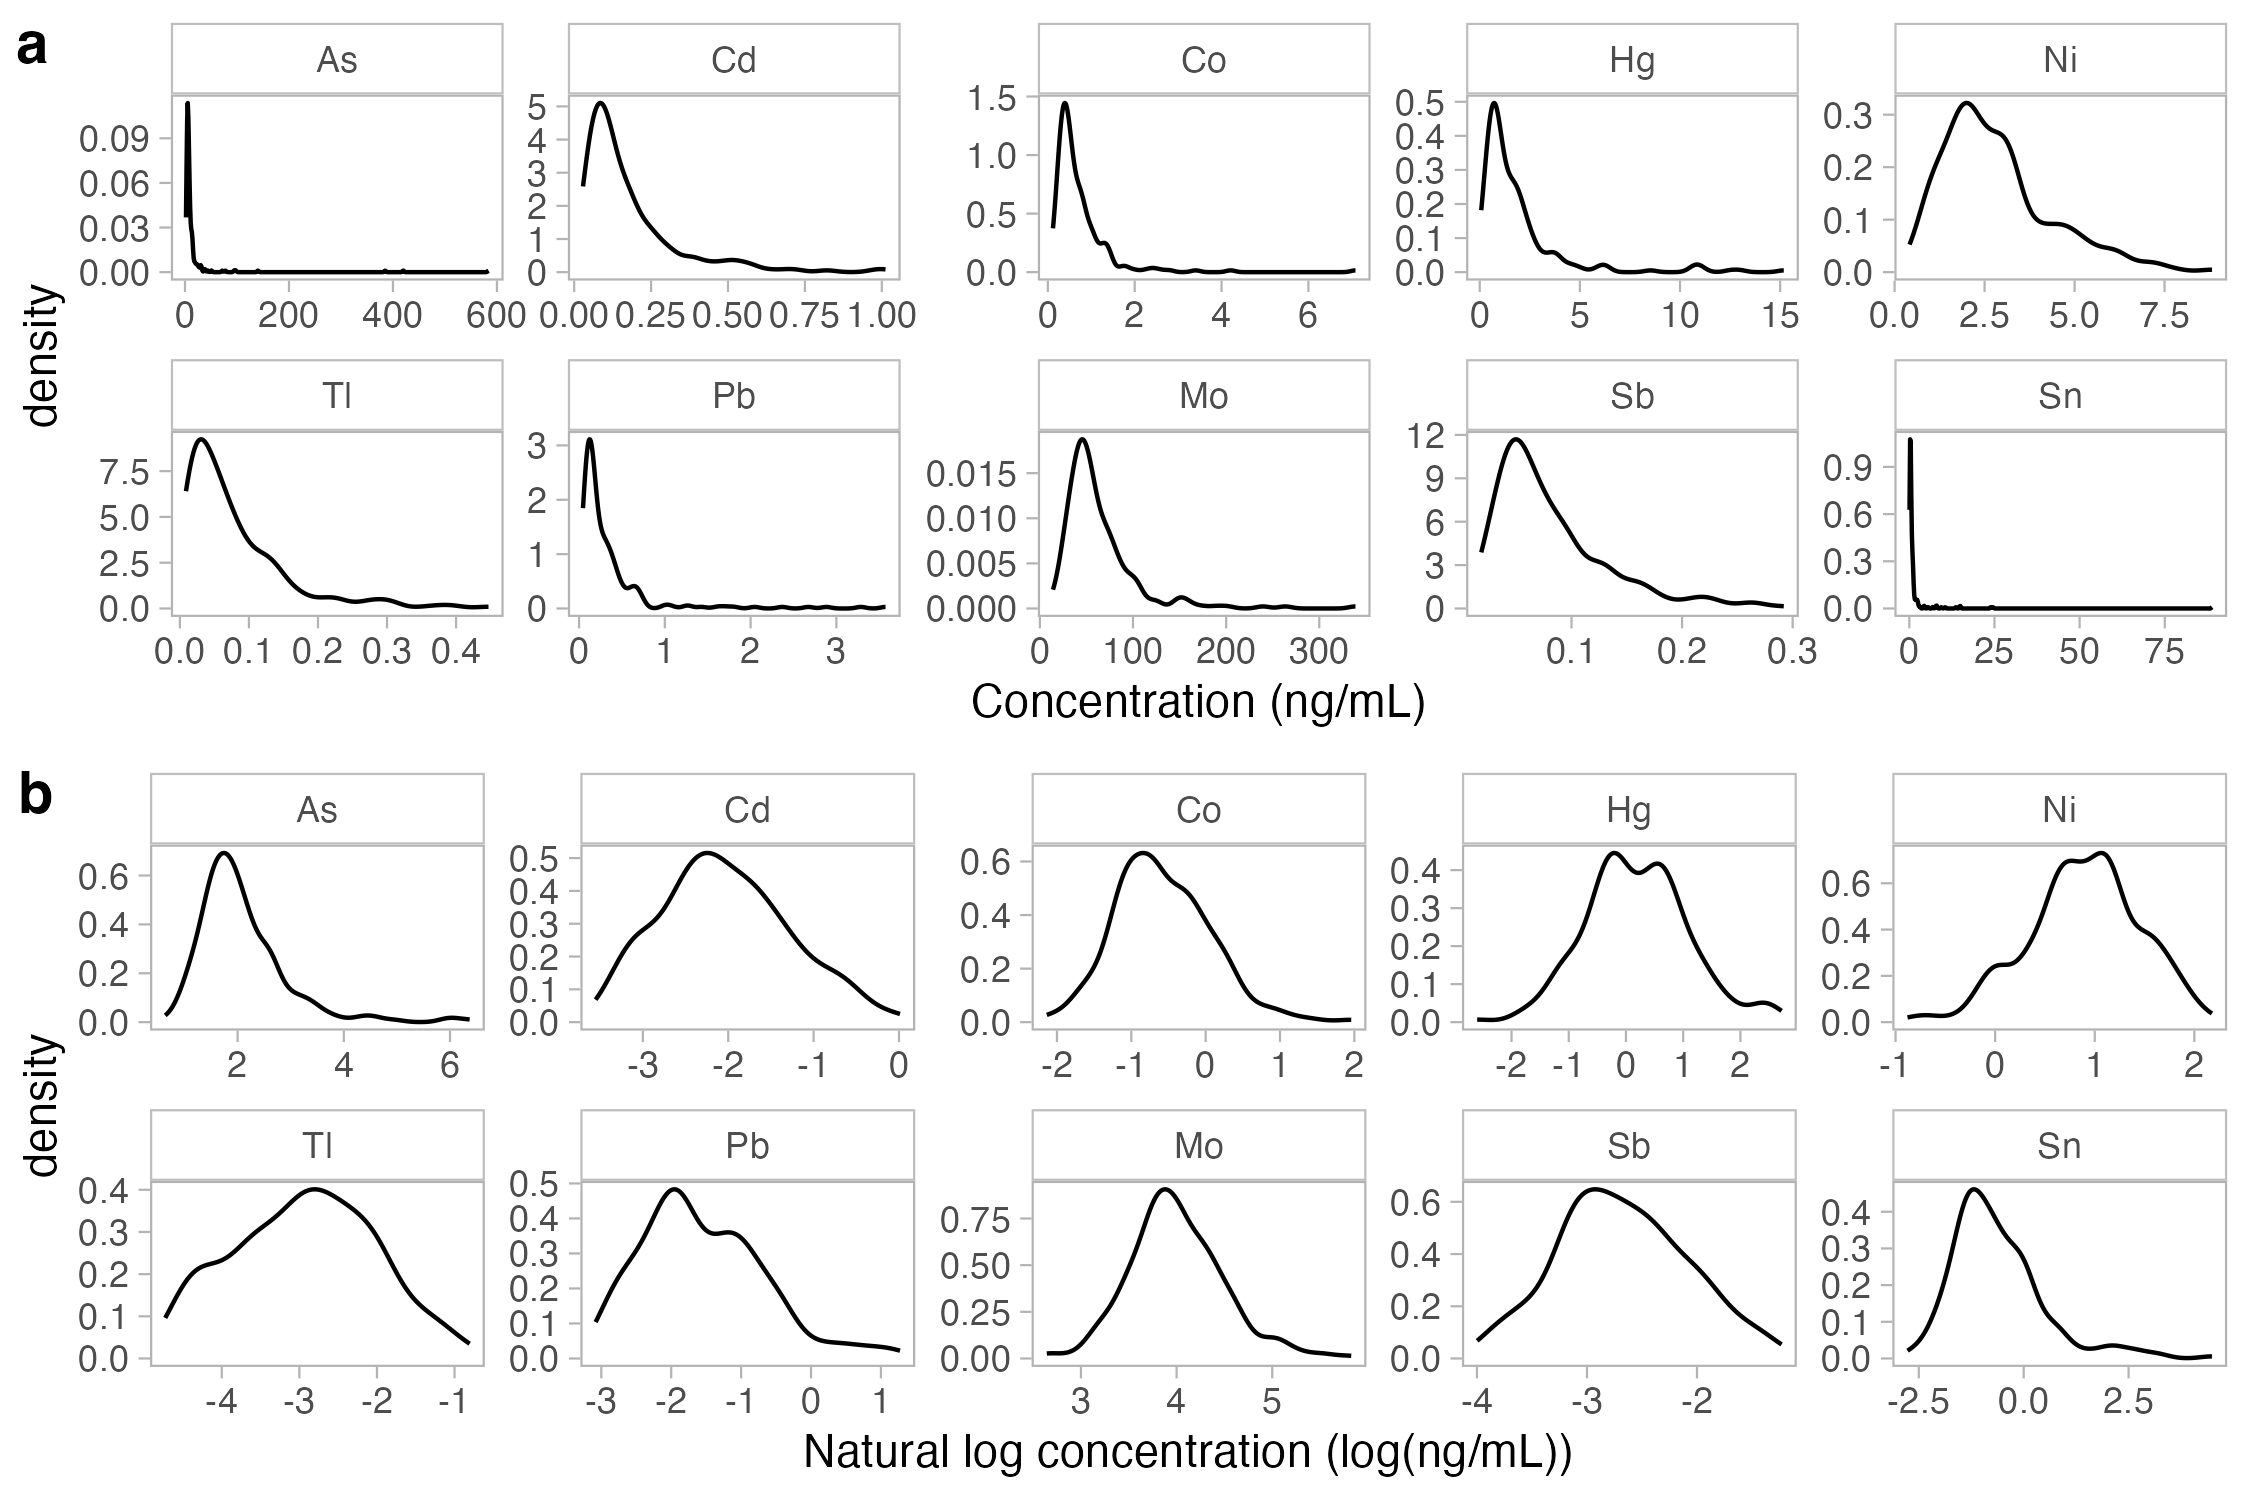
\includegraphics[width=0.9\linewidth]{figures/ch4_univlog} 

}

\caption{Distributions of original (a) and natural log transformed (b) concentrations of metals in MADRES cohort (n=252).}\label{fig:logtransf}
\end{figure}
We followed the approach by Howe et al. (\protect\hyperlink{ref-howe_prenatal_2020}{2020}) for preparing the data for analysis. This resulted in retaining 10 metals in analysis: arsenic (As), cadmium (Cd), cobalt (Co), mercury (Hg), nickel (Ni), molybdenum (Mo), lead (Pb), antimony (Sb), tin (Sn), and thallium (Tl). Howe et al. (\protect\hyperlink{ref-howe_prenatal_2020}{2020}) used speciated As, but this was not available in HHEAR, so we used total As. Metals were expressed in nanograms per milliliter (ng/mL) and natural log transformed to reduce right-skewness (Figure \ref{fig:logtransf}). Among the full range of covariates considered by Howe et al. (\protect\hyperlink{ref-howe_prenatal_2020}{2020}), we used the subset of 4 that were available in HHEAR: any smoke exposure during pregnancy, maternal prepregnancy body mass index (BMI), maternal age during firt trimester, and maternal race by ethnicity and birth place. We chose not to include study site, as there was a study site with only 1 participant. Race by ethnicity and birth place was collapsed into the following categories: non-Hispanic white, non-Hispanic black, non-Hispanic other, Hispanic born in the US, and Hispanic born outside the US. We observed 8 missing values for BMI in the data from HHEAR, which were not reported by Howe et al. (\protect\hyperlink{ref-howe_prenatal_2020}{2020}). We mean imputed these missing values. Distributions of covariates are shown in Figure \ref{fig:covdist}. Our final analytic dataset included 252 participants, which was 10 fewer than in Howe et al. (\protect\hyperlink{ref-howe_prenatal_2020}{2020}), likely due to small discrepancies in their dataset and the one made available in HHEAR.
\begin{figure}

{\centering 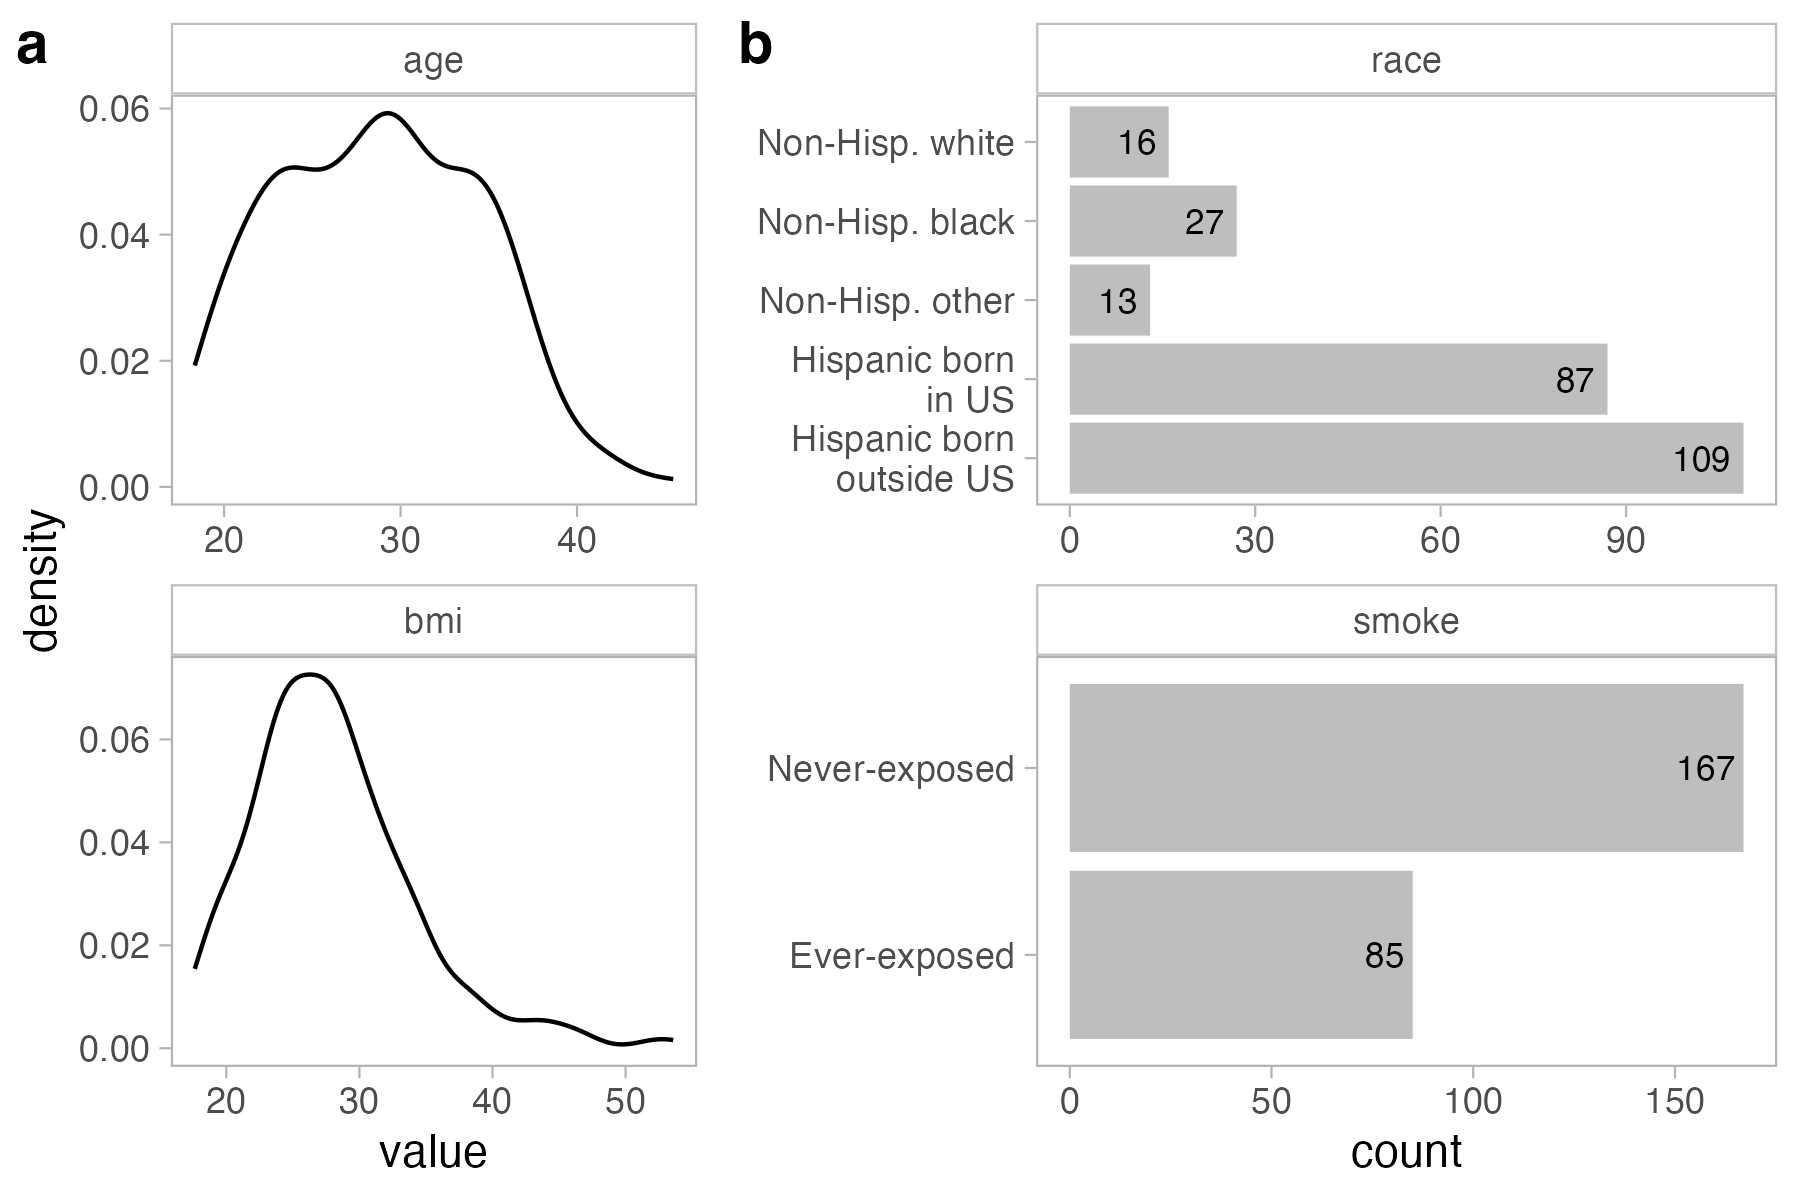
\includegraphics[width=0.75\linewidth]{figures/ch4_covdist} 

}

\caption{Distributions of continuous (a) and categorical (b) covariates in the MADRES cohort (n=252).}\label{fig:covdist}
\end{figure}
\hypertarget{copula}{%
\subsection{Using copulas to simulate predictor data}\label{copula}}

We simulated exposure and covariate data (hereafter referred to collectively as predictors) using a multivariate Gaussian copula fit on the 252 participants in the MADRES cohort. We used copulas as they can preserve both the correlation structure and marginal distributions from the observed data, allowing us to replicate conditions in a real-world scenario.

First, we briefly introduce copulas in the context of their use in this simulation, based on the presentation in Nelsen (\protect\hyperlink{ref-nelsen_introduction_2006}{2006}). Copulas are joint cumulative distribution functions (CDFs) defined on the unit cube \([0,1]^n\) that capture the dependence between \(n\) uniformly distributed marginals. Sklar's theorem allows us to apply copulas to our observed data. Sklar's theorem states that, if \(H(x_1, \dots x_n)\) is a joint CDF of the marginal CDFs \(F_1(x_1), \dots, F_n(x_n)\), then there exists a copula \(C\) such that, for all \((x_1, \dots, x_n)\) in \((X_1, \dots, X_n)\),

\[
H(x_1, \dots x_n)=C(F_1(x_1), \dots, F_n(x_n)).
\]

\noindent Note that, by the probability integral transform, or the universality of the uniform, the CDFs \(F_1(x_1), \dots, F_n(x_n)\) are distributed uniformly.

We used the \texttt{copula} package in R to fit copulas and generate random data (\protect\hyperlink{ref-hofert_copula_2023}{Hofert, Kojadinovic, Maechler, \& Yan, 2023}). We transformed the observed continuous predictor values to uniform distributions based on their empirical marginal CDFs, a process called generating ``pseudo-random'' samples. We used the checkerboard copula approach for generating pseudo-random samples for smoke exposure, a binary variable (\protect\hyperlink{ref-genest_primer_2007}{Genest \& Nešlehovà, 2007}). We coded smoke exposure as 0's and 1's, generated a pseudo-random sample, and then ``jittered'' the values with uniform random noise. There is currently no widely accepted approach for generating pseudo-random samples from unordered categorical variables with more than two levels. Thus, we excluded race by ethnicity and birthplace from the copula model. While this means that our simulated datasets did not preserve any potential association between race and exposures, Figure \ref{fig:raceexp} suggests that there is little to no visible association between race and exposures in the observed dataset.
\begin{figure}

{\centering 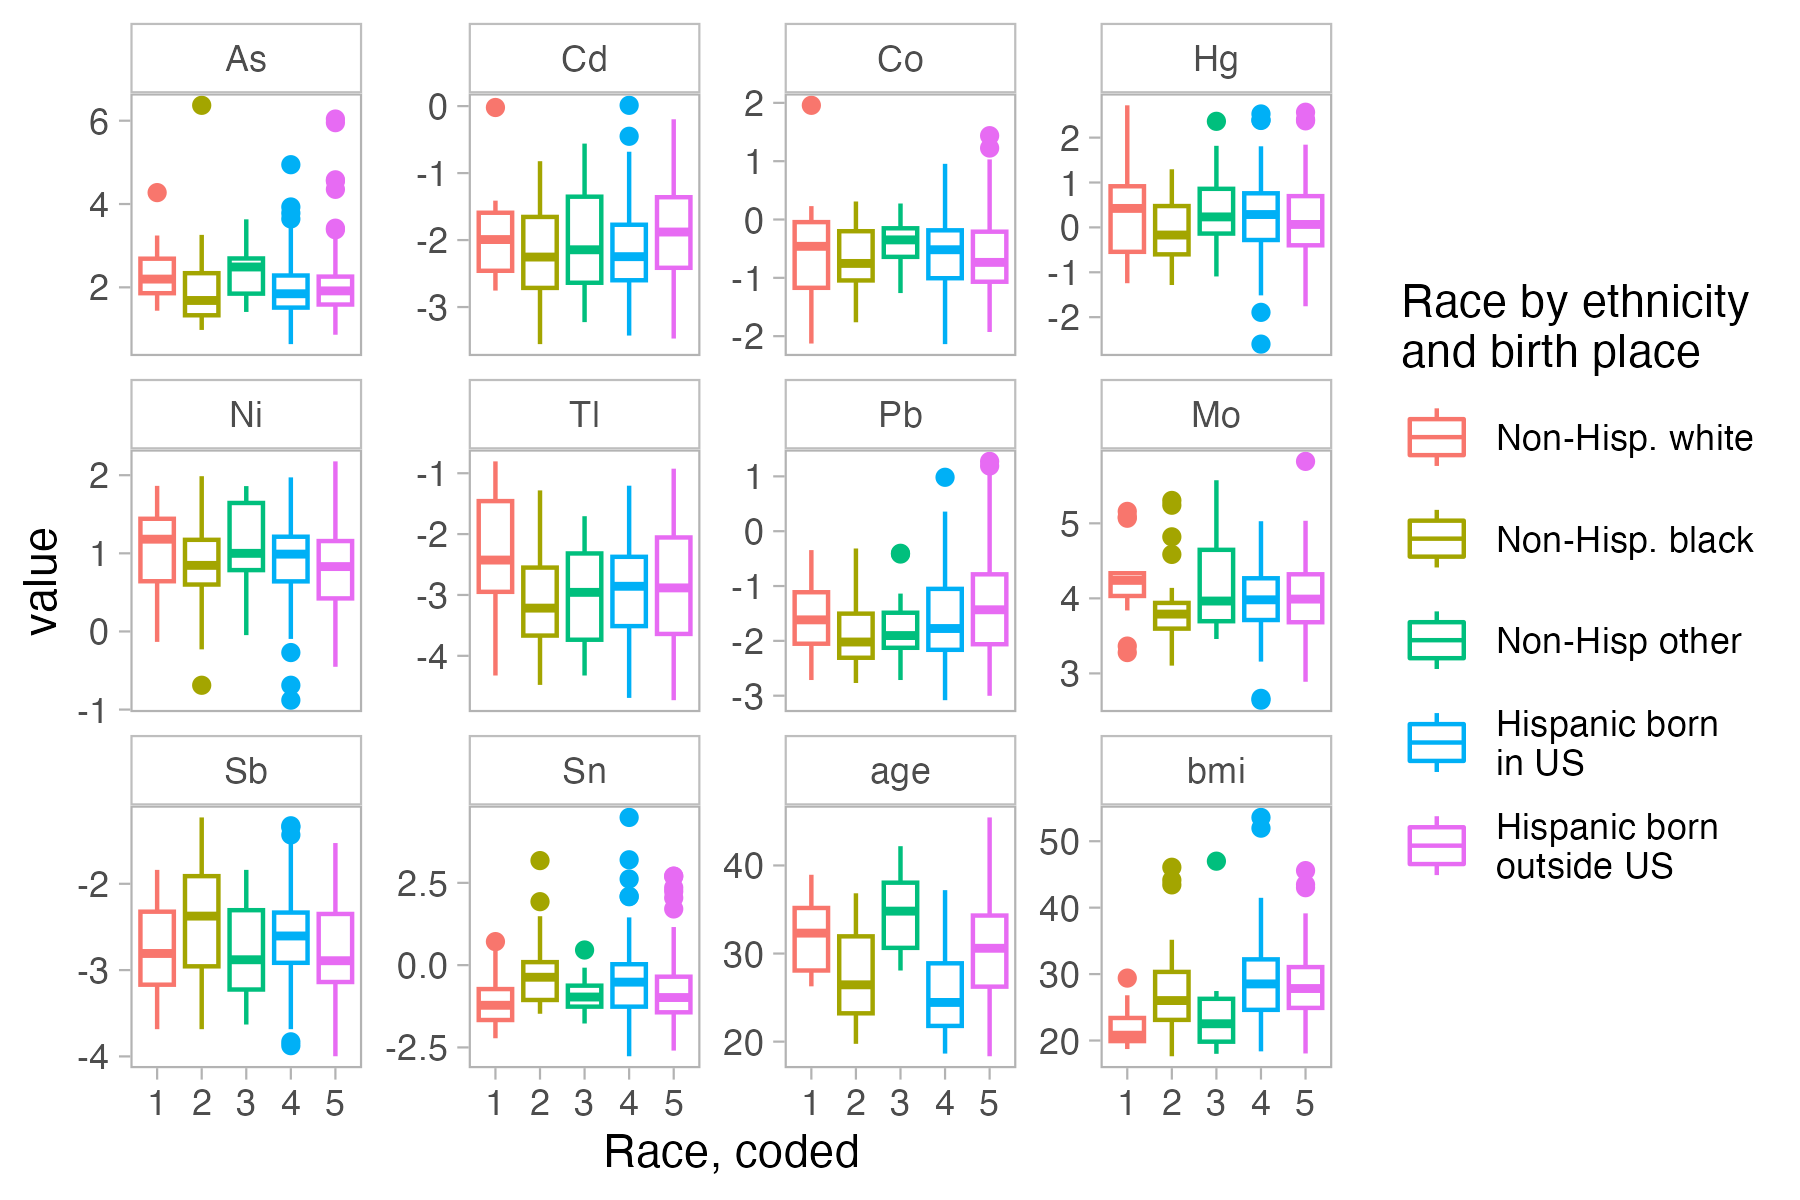
\includegraphics[width=0.8\linewidth]{figures/ch4_race_exp} 

}

\caption{Association between race by ethnicity and birth place and metal exposures in the MADRES cohort (n=252).}\label{fig:raceexp}
\end{figure}
Various families of copulas have been described, each of which specifies a different shape for the dependence structure. We performed model selection to identify the copula that best approximates the dependence structure of our data. We fit the set of multivariate copulas used by Lazarevic et al. (\protect\hyperlink{ref-lazarevic_performance_2020}{2020}) in their simulation study, which included the Gaussian, \(t\), Gumbel, Frank, Clayton, and Joe copulas. We fit two \(t\) copulas with 4 and 10 degrees of freedom, which controls dependence at the tails of the distributions, as well as a \(t\) copula where the degrees of freedom was determined during the fitting process. The Gumbel, Frank, Clayton, and Joe copulas require a \(\theta\) parameter, which controls dependence between the distributions. We fit two versions of these copulas with \(\theta=\{2, 4\}\). Among these, the Gaussian copula minimized the Akaike information criterion and maximized the likelihood, so we proceeded with this model. The Gaussian copula assumes a bivariate normal dependence structure between the marginal CDFs.
\begin{figure}

{\centering 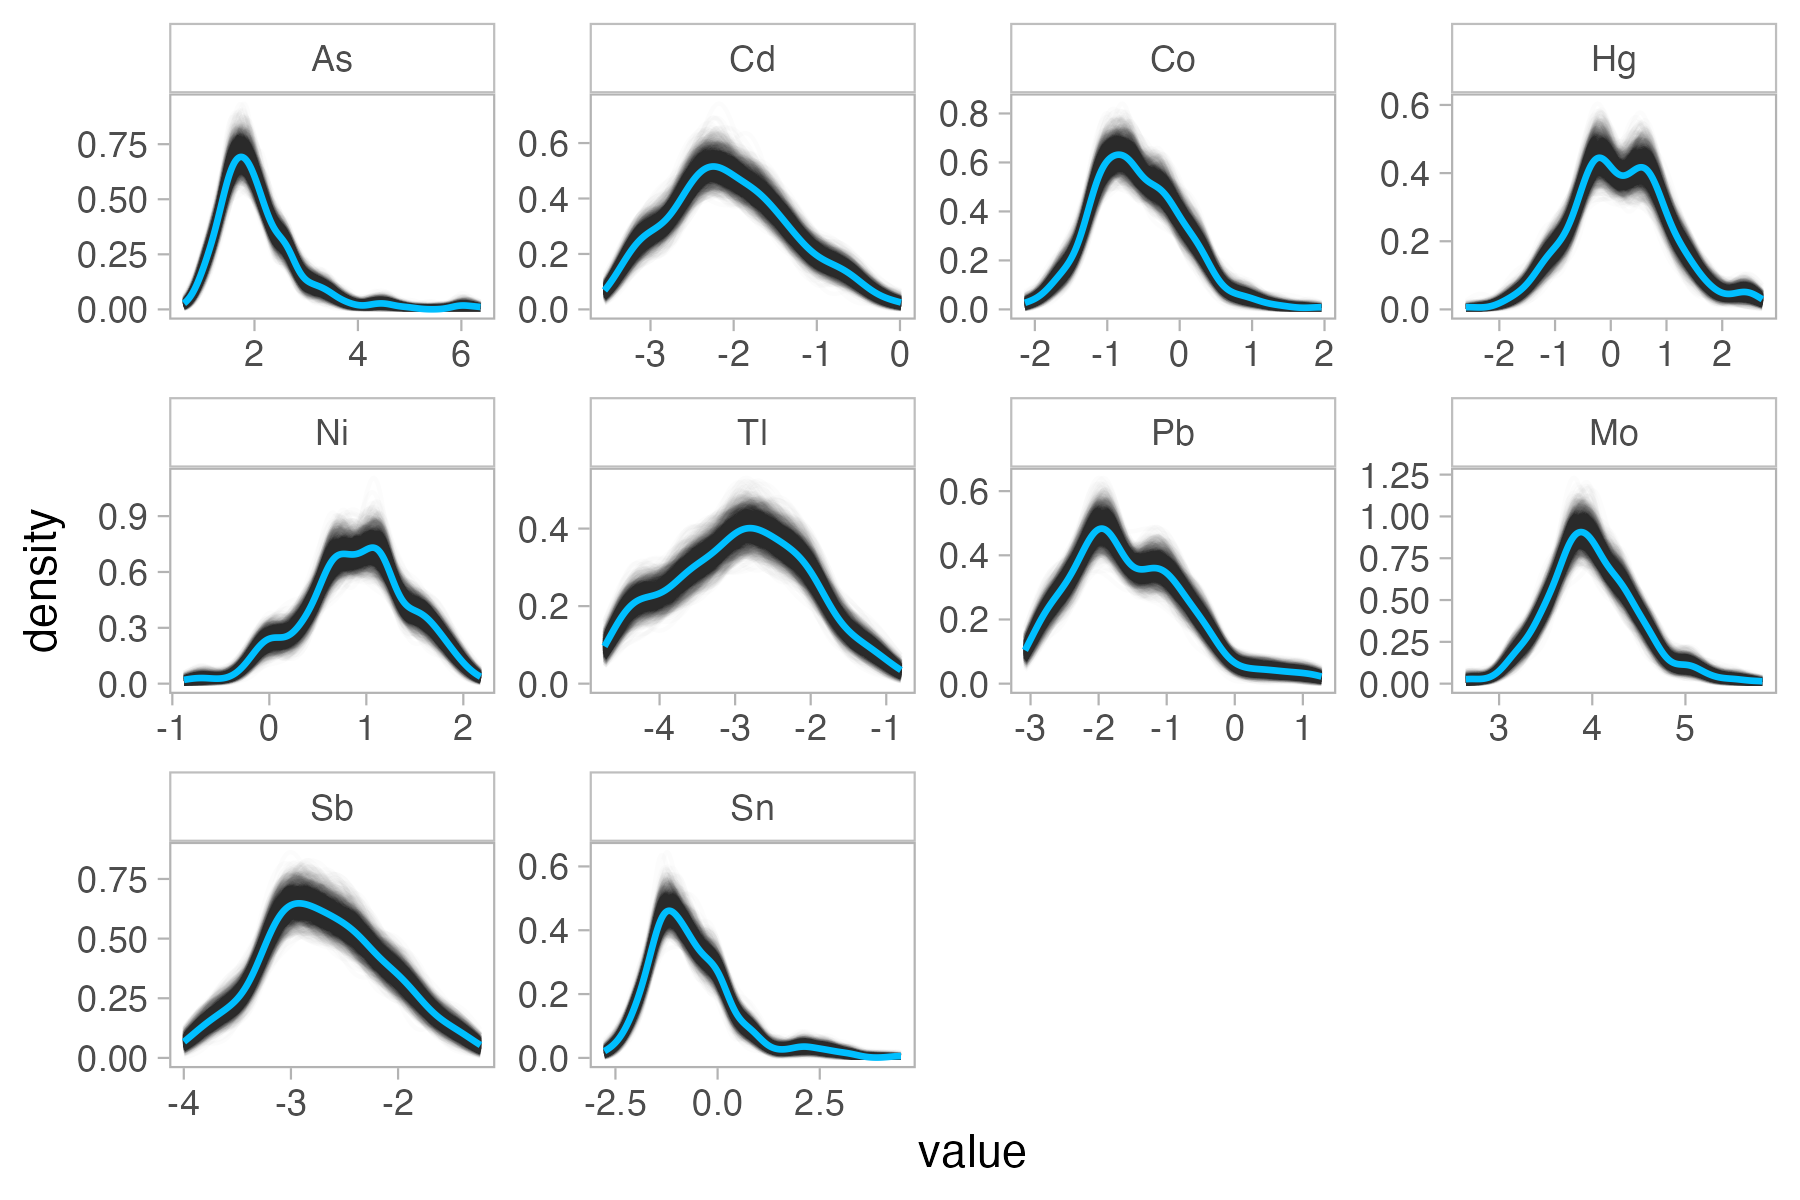
\includegraphics[width=0.75\linewidth]{figures/ch4_univ_exp_sim} 

}

\caption{Distributions of log-transformed exposures from observed data (blue) and 2100 simulated smaller size (n=252) datasets (gray).}\label{fig:univexpsim}
\end{figure}
\begin{figure}

{\centering 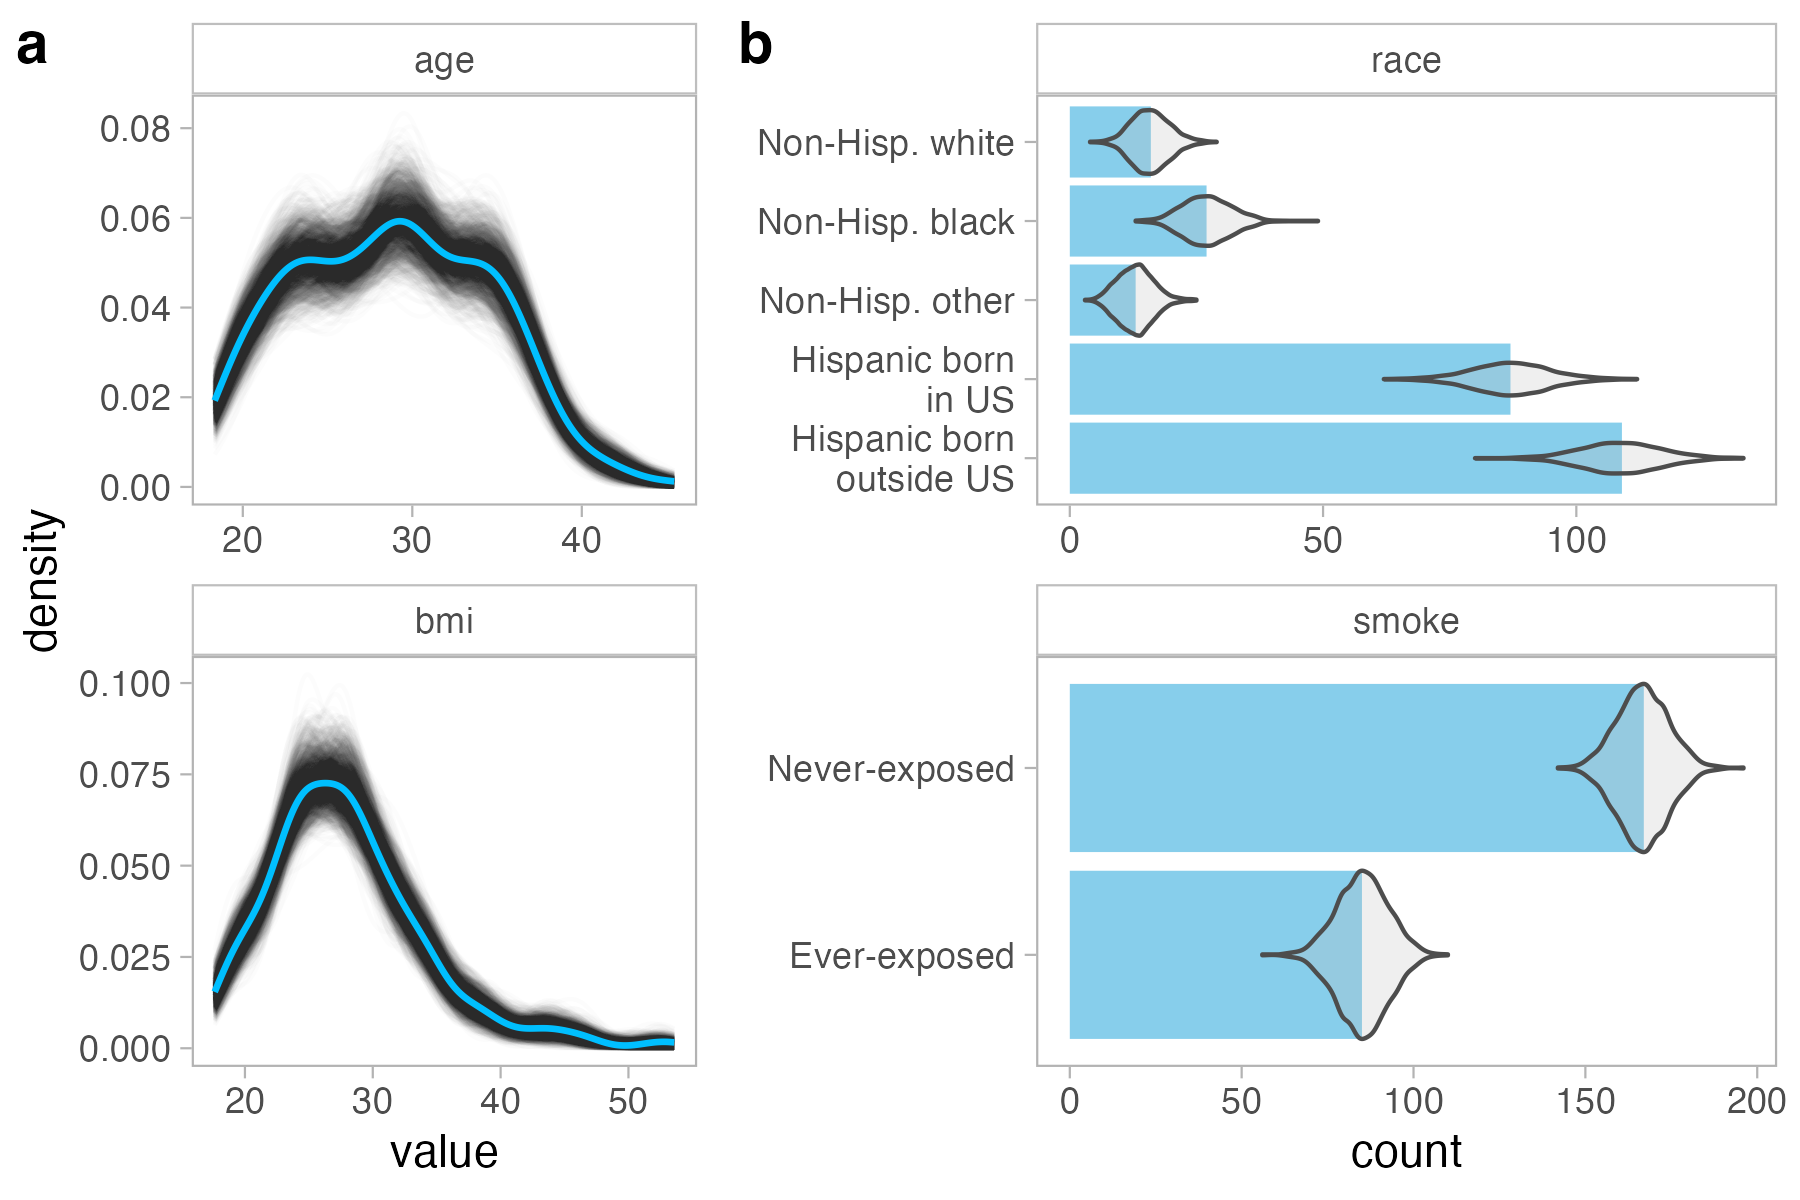
\includegraphics[width=0.75\linewidth]{figures/ch4_univ_cov_sim} 

}

\caption{Distributions of continuous (a) and categorical (b) covariates from observed data (blue) and 2100 simulated smaller size (n=252) datasets (gray).}\label{fig:univcovsim}
\end{figure}
We simulated predictor data by randomly sampling from the fitted multivariate Gaussian copula distribution. All pseudo-random samples were then back-transformed to their original distributions using empirical marginal CDFs. We simulated the race by ethnicity and birthplace variable by randomly assigning observations to each of the five categories based on proportions in the observed dataset.
\begin{figure}

{\centering 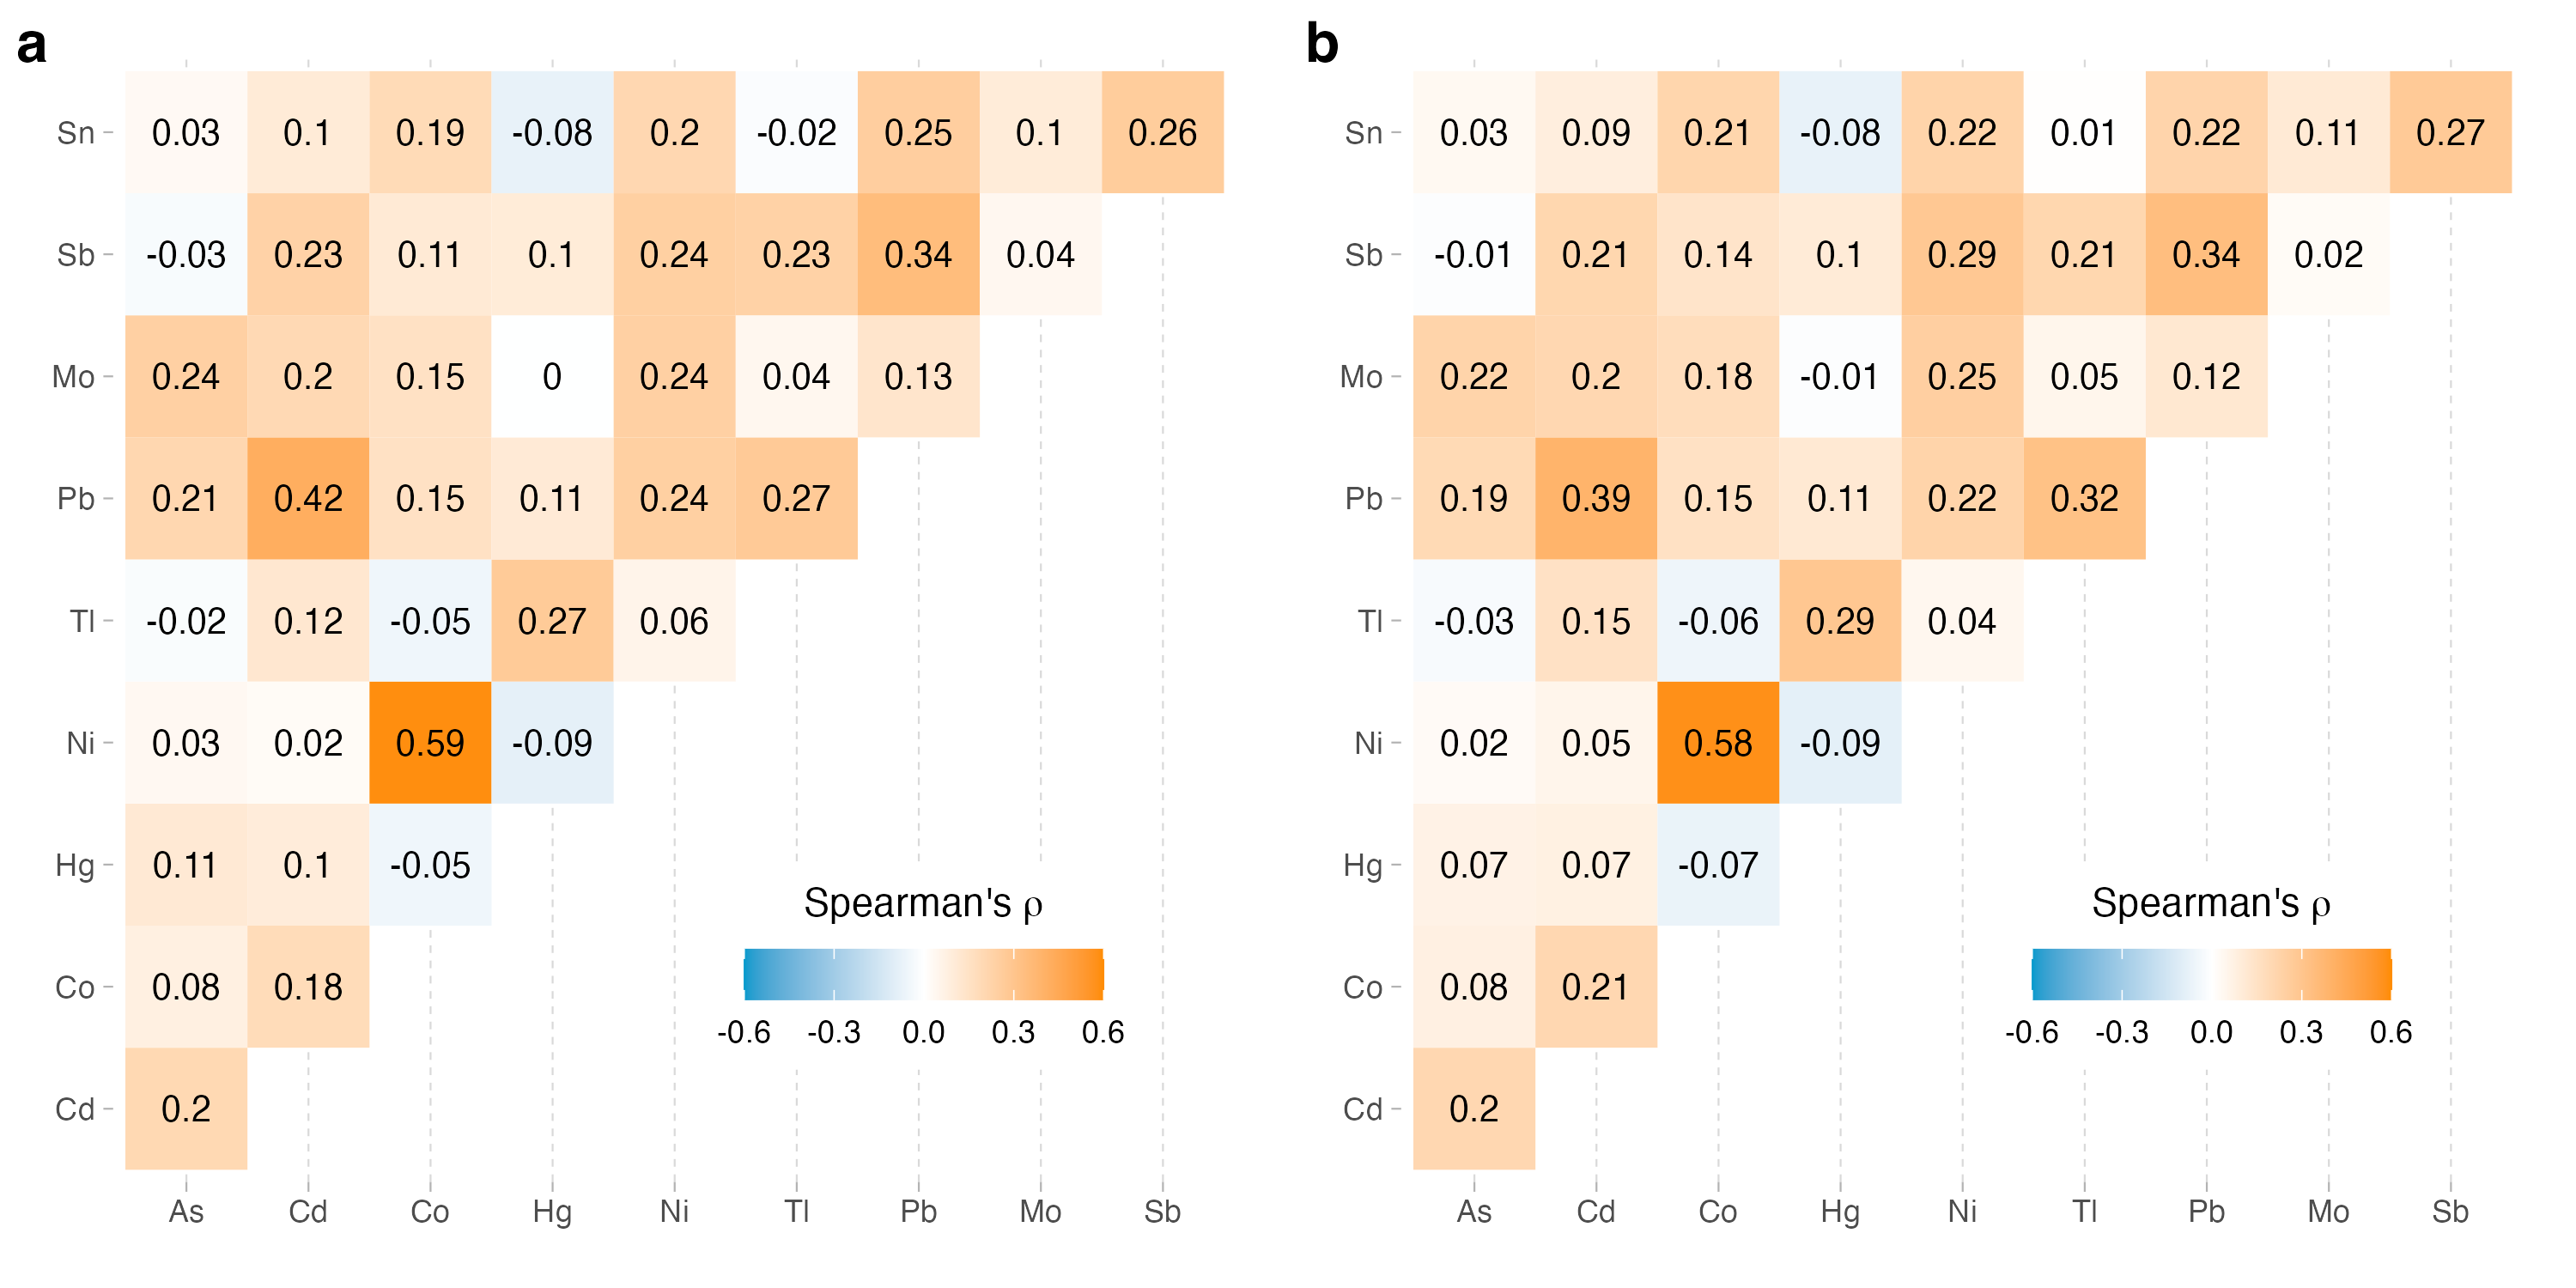
\includegraphics[width=1\linewidth]{figures/ch4_corr_sim+orig} 

}

\caption{Spearman's correlation heat maps of exposures from observed data (a) and averaged across 2100 smaller size (n=252) simulated datasets (b).}\label{fig:corsimssm}
\end{figure}
We generated one set of simulated datasets with the same sample size as the observed dataset (n=252), which is typical in many cohort studies. We also generated another set of simulated datasets with a larger sample size (n=1000), which has become increasingly common with the rise of larger-scale studies. The goal of this choice was to inform sample size considerations in study design. We verified that the original structure of the observed dataset were preserved by visually comparing univariate distributions of exposures (Figure \ref{fig:univexpsim}) and covariates (Figure \ref{fig:univcovsim}), as well as the correlation structure using Spearman's \(\rho\) (Figure \ref{fig:corsimssm}). Distributions of Spearman's correlation were approximately normal (Figure \ref{fig:cordistsm}). Plots for the larger size simulated datasets were similar (Figures \ref{fig:univexplg}, \ref{fig:univcovlg}, and \ref{fig:corsimslg}).

\hypertarget{simresp}{%
\subsection{Simulating predictor-response relationships}\label{simresp}}

Health outcome responses were simulated under several different scenarios, each of which included different effect sizes and functional forms for the interactions. All scenarios were run for both the smaller (n=252) and larger (n=1000) sample sizes. In the first scenario, we specified a ``base case'' model:
\begin{multline*}
Y = \textrm{Hg} + \frac{3}{1+\textrm{exp}(-4\textrm{Ni})} + \frac{1.5}{1+\textrm{exp}(-4\textrm{Sn})} - \textrm{Sb}^2 + 0.5\textrm{Sb}\\
+ \textrm{age} + 0.5\textrm{bmi} + 0.5\textrm{race}_{\textrm{black}} + 0.5\textrm{race}_{\textrm{hisp.non}} + 1.5\textrm{smoke} + \varepsilon,
\end{multline*}
\noindent where \(\varepsilon \overset{\mathrm{iid}}{\sim} N(0,5)\). This model includes a linear term for Hg, two S-shaped logistic terms for Ni and Sn with varying effect sizes, and a symmetric inverse U-shaped quadratic term for Sb (Figure \ref{fig:univlines}). Moreover, we included covariate terms as linear effects in the model. We chose the standard deviation on the normal random error term in order to achieve an \(R^2\) of around 0.1-0.3 in a multiple linear regression that included only the true functional form of the significant chemicals (Figure \ref{fig:rsqcheck}). This \(R^2\) range approximates realistic signal-to-noise ratios in exposure mixture studies (\protect\hyperlink{ref-lazarevic_performance_2020}{Lazarevic et al., 2020}).

In subsequent scenarios, we added an additional interaction term to the base case model. First, we considered interactions between two exposures. We defined four cases of interest: a two-way interaction between exposures that are univariately significant, a two-way interaction between exposures that are univariately insignificant, a two-way interaction between exposures that are moderately collinear, and a three-way interaction. For each case, we considered two functional forms --- multiplicative and polynomial --- and a lower and higher effect size, which we set by defining the weight on the interaction term in the model. The higher effect sizes were selected in order to achieve a power of approximately 0.5 at \(\alpha=0.05\) in the smaller sample size (n=252) case, using a multiple linear regression with the true functional form of the chemicals specified and the covariate terms included. The lower effect sizes were set equal to half of the higher effect size. Table \ref{tab:scenarios} shows the specification of interaction terms. See Appendix \ref{suppmethods}, Figures \ref{fig:basesurf}-\ref{fig:cp2}, for 3D surfaces of the two-way interaction terms.
\begin{table}

\caption{\label{tab:scenarios}Specification of interaction terms in simulations.}
\centering
\begin{tabular}[t]{>{\raggedright\arraybackslash}p{10em}cc}
\toprule
\multicolumn{1}{c}{ } & \multicolumn{2}{c}{Effect size} \\
\cmidrule(l{3pt}r{3pt}){2-3}
 & Lower & Higher\\
\midrule
\addlinespace[0.3em]
\multicolumn{3}{l}{\textbf{Univariately significant}}\\
\hspace{1em}Multiplicative & 0.35Hg$*$Ni & 0.7Hg$*$Ni\\
\hspace{1em}Polynomial & 0.13Hg$*($Ni$-1)^2$ & 0.26Hg$*($Ni$-1)^2$\\
\addlinespace[0.3em]
\multicolumn{3}{l}{\textbf{Univariately insignificant}}\\
\hspace{1em}Multiplicative & 0.35Cd$*$As & 0.7Cd$*$As\\
\hspace{1em}Polynomial & 0.125Cd$*($As$-1)^2$ & 0.25Cd$*($As$-1)^2$\\
\addlinespace[0.3em]
\multicolumn{3}{l}{\textbf{Highly correlated}}\\
\hspace{1em}Multiplicative & 0.3Ni$*$Co & 0.6Ni$*$Co\\
\hspace{1em}Polynomial & 0.1Ni$*($Co$-1)^2$ & 0.2Ni$*($Co$-1)^2$\\
\addlinespace[0.3em]
\multicolumn{3}{l}{\textbf{Three-way interaction}}\\
\hspace{1em}Multiplicative & 0.3Hg$*$Ni$*$Tl & 0.6Hg$*$Ni$*$Tl\\
\hspace{1em}Polynomial & 0.09Hg$*($Ni$-1)^2*$Tl & 0.18Hg$*($Ni$-1)^2*$Tl\\
\bottomrule
\end{tabular}
\end{table}
Next, we considered interactions between the race by ethnicity and birthplace covariate (hereafter referred to as race for concision) and an exposure. We are interested in cases where the health effects of an exposure are higher in one group compared to the rest. In a real-world scenario, such interactions can arise from excess amounts of social stress experienced by a group due to racism. To model this, we increased the coefficient Hg in Non-Hispanic Black individuals (n=27 in the original MADRES cohort) for the first scenario, and in Hispanic individuals born outside the US (n=109 in the original MADRES cohort) for the second scenario. The goal of this choice was to assess the impact of group size on detectability of an interaction, and to quantify the potential value of oversampling the minority group. For each scenario, we specified a lower effect size by increasing the coefficient on Hg by \(1.5\times\) (i.e.~from \(1*\)Hg to \(1.5*\)Hg) in the target group, and a higher effect size by increasing the coefficient on Hg by \(2\times\) (i.e.~from \(1*\)Hg to \(2*\)Hg).

This resulted in a total of 42 scenarios ({[}1 base case + 5 interaction cases \(\times\) 2 effect sizes \(\times\) 2 functional forms{]} \(\times\) 2 sample sizes = 42). For each scenario, we generated 100 simulated datasets to fit our models on, resulting in a total of 4200 datasets. Hereafter, we refer to the two different effect sizes of interactions using ``lower'' and ``higher,'' and we refer to the two different sample sizes as ``small'' and ``large,'' or ``smaller'' and ``larger.''

\hypertarget{models}{%
\subsection{Models}\label{models}}

We ran four methods on our simulated datasets. All metal concentrations and continuous covariates were standardized in analysis to keep values scale-free.

To get a baseline, we ran a multiple linear regression, including all exposures and covariates as linear, additive terms in the model. We refer to this model as the naive MLR. Then, we ran a multiple linear regression with the true model explicitly specified by excluding non-significant exposures and specifying the known form of non-linear terms and non-additive interactions. We refer to this model as the oracle MLR. In scenarios with an interaction between race and Hg, we collapsed race into a binary variable indicating whether or not the original race category was interacting with Hg before running oracle MLR's, in order to simplify the detection of the interaction.

Next, we ran BKMR using the \texttt{bkmr} package in R (\protect\hyperlink{ref-bobb_bkmr_2022}{Bobb, 2022}; \protect\hyperlink{ref-bobb_statistical_2018}{Bobb et al., 2018}). We chose to implement component-wise variable selection rather than hierarchical selection to make simulation results more interpretable, and because there was only moderate multicollinearity in the observed and simulated data. We specified the default priors (\protect\hyperlink{ref-bobb_bayesian_2015}{Bobb et al., 2015}, and as listed in Chapter \ref{bkmrprior}), which is common in the literature for BKMR Pesenti et al. (\protect\hyperlink{ref-pesenti_comparative_2023}{2023}). We ran the MCMC sampler for 50,000 iterations, as recommended by Bobb et al. (\protect\hyperlink{ref-bobb_statistical_2018}{2018}), and discarded the first 25,000 iterations for burn-in. BKMR does not provide the option to run multiple chains or to thin chains. For larger size datasets, we sped up computations by employing a Gaussian predictive process on 100 knots specified evenly across the predictor space.

We ran BSR using the \texttt{NLinteraction} package in R (\protect\hyperlink{ref-antonelli_nlinteraction_2018}{Antonelli, 2018}). We specified the default priors (\protect\hyperlink{ref-antonelli_estimating_2020}{Antonelli et al., 2020}, and as listed in Chapter \ref{bsrprior}), which is common in the literature for BSR (e.g., \protect\hyperlink{ref-howe_prenatal_2020}{Howe et al., 2020}; \protect\hyperlink{ref-pesenti_comparative_2023}{Pesenti et al., 2023}). Antonelli et al. (\protect\hyperlink{ref-antonelli_estimating_2020}{2020}) suggests separately fitting models for degrees of freedom \(d=\{1, 2, 3, 4\}\) and selecting the value for \(d\) which minimizes WAIC. We used the default Gibbs sampler, as opposed to the Metropolis Hasting sampler. Due to time constraints in this thesis, we first fit BSR on the grid of values for \(d\) using 5,000 MCMC iterations to obtain the empirical Bayes estimate for \(\sigma^2_{\boldsymbol\beta}\) and then another 5,000 MCMC iterations to obtain the posterior distributions, discarding the first 2,500 iterations for burn-in each time. We selected \(d\) based on the WAIC criterion on these preliminary models. Then, we fit the full BSR model using 50,000 MCMC iterations to obtain the empirical Bayes estimate and then another 50,000 MCMC iterations to obtain the posterior distributions, discarding the first 25,000 iterations for burn-in each time. We ran two chains to verify convergence, thinning each chain by selecting every 8th iteration to reduce autocorrelation based on default settings. In a small test run on five smaller size datasets for each scenario containing interactions between exposures, as well as the base case, we found that using 5,000 iterations selected the same degrees of freedom as using 50,000 iterations 86\% of the time (see Appendix \ref{suppmethods}, Figure \ref{fig:comparedf}).

Finally, we ran stratified BKMR and BSR models in scenarios where we simulated an interaction between race and Hg. This involved running five separate models for each race category, each with the same settings specified above. For the smaller size datasets, we often observed convergence issues in BKMR within the smaller race categories. As such, for smaller size datasets, we also assess the impact of collapsing the three smaller race categories (Non-Hispanic white, black, and other) into one category before stratifying. This is a common practice in real-world studies where sample sizes for certain categories are low.

For all models, we saved run-times for the fitting process on the high-performance computing cluster. Due to an error in our code and time constraints in this thesis, we were not able to obtain run times for stratified BSR models. We checked convergence for a selection of BKMR and BSR models using trace plots (Appendix \ref{suppresults}, Figure \ref{fig:traceplots}).

\hypertarget{model-assessment}{%
\subsection{Model assessment}\label{model-assessment}}

We assessed model performance based on detection of significant univariate chemicals as well as detection of interactions. For the naive and oracle MLRs, we considered a \(p\)-value less than 0.05 to indicate detection of a significant term. For BKMR and BSR, we used the median probability model, which considers a PIP greater than or equal to 0.5 to indicate detection of a significant term (\protect\hyperlink{ref-barbieri_optimal_2004}{Barbieri \& Berger, 2004}).

While BSR provides PIP's to quantify detection of interactions, BKMR does not. As such, for BKMR, we considered formal detection of an interaction based on confidence intervals constructed around the estimated response. Specifically, we first calculated the difference in estimated response at a chemical's 0.25 and 0.75 quantiles. Then, we assessed whether this quantity differed at the 0.25 and 0.75 quantiles of one (or two, for three-way interactions) other chemicals in the interaction, while holding all other chemicals at their 0.5 quantiles, by constructing a 95\% confidence interval of the difference in differences. We followed the code in the \texttt{SingVarIntSummaries()} function in the \texttt{bkmr} package for constructing confidence intervals (\protect\hyperlink{ref-bobb_bkmr_2022}{Bobb, 2022}). Notably, for two-way interactions, the ordering of the chemicals in this comparison does not matter. To see why, see \eqref{eq:confinteq} in Appendix \ref{suppmethods}. However, for three-way interactions, the order does matter. Thus, we considered a three-way interaction to be detected if at least one of the three confidence intervals was significantly greater than zero. We used the Bonferroni correction to adjust for multiple comparisons, creating 98.3\% confidence intervals to achieve an overall 95\% confidence level (\protect\hyperlink{ref-dunn_multiple_1961}{Dunn, 1961}; \protect\hyperlink{ref-vanderweele_desirable_2019}{VanderWeele \& Mathur, 2019}).

For both BKMR and BSR, we also visually assessed detection of interactions by plotting the estimated exposure-response surface for one chemical while fixing one (or two, for three-way interactions) other chemicals at their 0.1, 0.5, and 0.9 quantiles. In all scenarios, we calculated the sensitivity as the proportion of times a significant term was correctly detected. Due to time constraints in this thesis, we only calculated the false discovery rates, or, the proportion of times a significant term is incorrectly detected, for two-way interactions between chemicals.

For stratified models, we compared the estimated response across each separate model. Specifically, for BKMR, we computed a confidence interval for the difference in estimated response at the 0.25 and 0.75 quantiles of Hg on each subcategory of race, following the code in the \texttt{SingVarRiskSummaries()} function in the \texttt{bkmr} package (\protect\hyperlink{ref-bobb_bkmr_2022}{Bobb, 2022}). We adjusted for multiple comparisons based on the Bonferroni procedure by constructing 5 simultaneous 99\% confidence intervals, in order to achieve an overall 95\% confidence level (\protect\hyperlink{ref-dunn_multiple_1961}{Dunn, 1961}; \protect\hyperlink{ref-vanderweele_desirable_2019}{VanderWeele \& Mathur, 2019}). We considered an interaction as correctly detected if (1) there was at least one overlap between the target group's confidence interval and all other confidence intervals, and (2) all other confidence intervals overlapped.

However, for BSR, we were not able to find a method in the literature for combining variances from estimated responses at two different sets of predictor values. While the kernel machine regression method used by BKMR generates a covariance matrix for estimates at various predictor values, which are then used to generate confidence intervals, the same is not true for the spline regression method used by BSR. Therefore, we visualized and compared the estimated exposure-response relationship in each of the stratified models as a qualitative way to assess for interactions. We also generated these diagnostic plots for BKMR. Moreover, due to time constraints in this thesis, we only considered sensitivity, as opposed to also considering false discovery rates.

See Appendix \ref{extractresults} for the code we wrote to extract some of the aforementioned results from BKMR and BSR, as some functions were not directly available from the \texttt{bkmr} and \texttt{NLinteraction} packages (\protect\hyperlink{ref-antonelli_nlinteraction_2018}{Antonelli, 2018}; \protect\hyperlink{ref-bobb_bkmr_2022}{Bobb, 2022}).

\hypertarget{results}{%
\section{Results}\label{results}}

\hypertarget{base-case}{%
\subsection{Base case}\label{base-case}}

We start by presenting results from models run on the base case scenario, in which the true relationship contained no interactions. Figure \ref{fig:basecasesig} displays the distribution of p-values and PIPs from this scenario, while Table \ref{tab:basecasetab} summarizes model sensitivity and false discovery rates based on these values. Note that insignificant chemicals were not included in the oracle MLR, which is why their distributions are omitted from this output.
\begin{figure}

{\centering 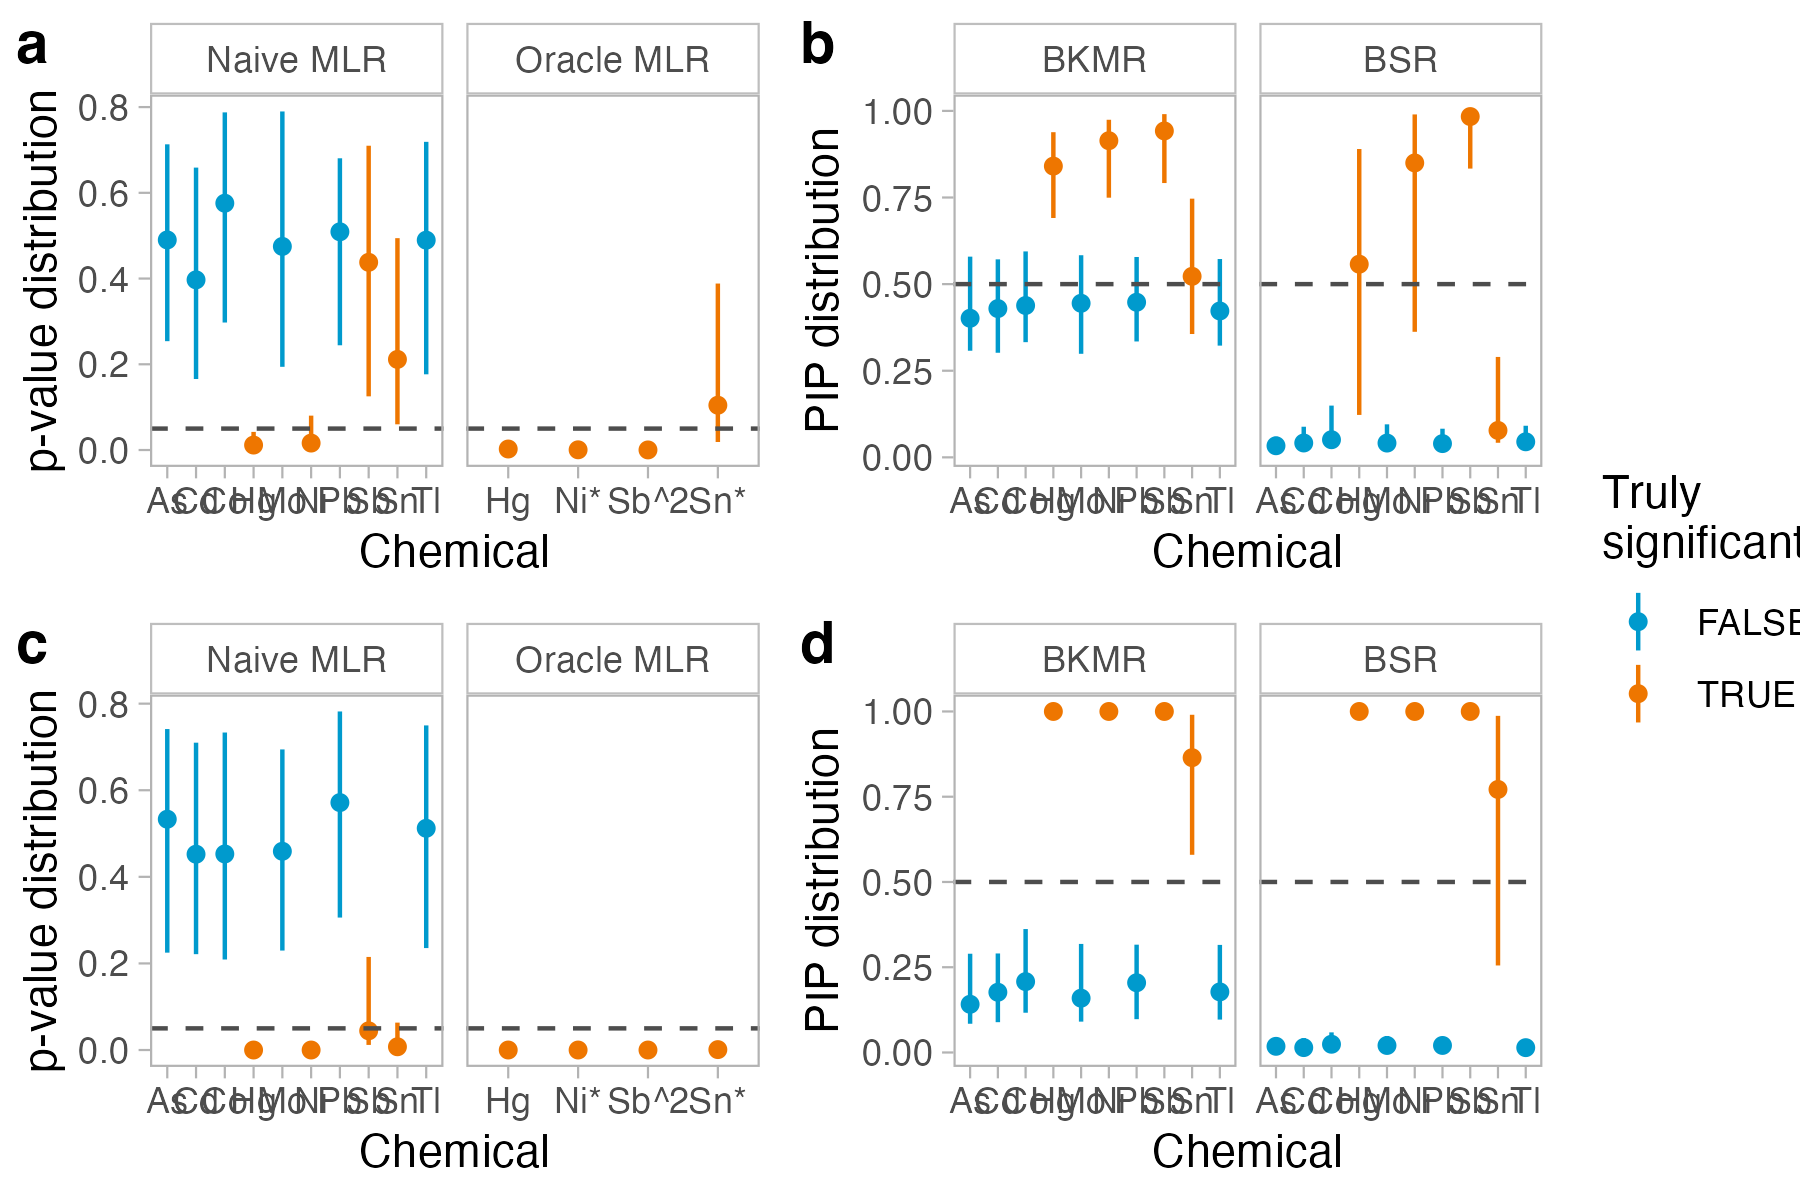
\includegraphics[width=1\linewidth]{figures/ch4_basecasesig} 

}

\caption{P-value distributions from smaller (a) and larger (b) size datasets and PIP distributions from smaller (c) and larger (d) size datasets.}\label{fig:basecasesig}
\end{figure}
\begin{table}

\caption{\label{tab:basecasetab}Sensitivity and false discovery rate (FDR) of chemicals in base case scenario.}
\centering
\begin{tabular}[t]{>{\raggedright\arraybackslash}p{6em}cccccccccc}
\toprule
\multicolumn{1}{c}{ } & \multicolumn{4}{c}{Sensitivity} & \multicolumn{6}{c}{FDR} \\
\cmidrule(l{3pt}r{3pt}){2-5} \cmidrule(l{3pt}r{3pt}){6-11}
 & Hg & Ni & Sb & Sn & As & Cd & Co & Mo & Pb & Tl\\
\midrule
\addlinespace[0.3em]
\multicolumn{11}{l}{\textbf{Naive MLR}}\\
\hspace{1em}Small & 0.80 & 0.70 & 0.12 & 0.24 & 0.05 & 0.07 & 0.02 & 0.07 & 0.03 & 0.08\\
\hspace{1em}Large & 1.00 & 1.00 & 0.51 & 0.71 & 0.02 & 0.04 & 0.08 & 0.13 & 0.03 & 0.03\\
\addlinespace[0.3em]
\multicolumn{11}{l}{\textbf{Oracle MLR}}\\
\hspace{1em}Small & 0.84 & 0.94 & 0.95 & 0.35 & - & - & - & - & - & -\\
\hspace{1em}Large & 1.00 & 1.00 & 1.00 & 0.89 & - & - & - & - & - & -\\
\addlinespace[0.3em]
\multicolumn{11}{l}{\textbf{BKMR}}\\
\hspace{1em}Small & 0.86 & 0.92 & 0.95 & 0.52 & 0.30 & 0.33 & 0.36 & 0.38 & 0.41 & 0.40\\
\hspace{1em}Large & 1.00 & 1.00 & 1.00 & 0.77 & 0.12 & 0.12 & 0.14 & 0.13 & 0.08 & 0.13\\
\addlinespace[0.3em]
\multicolumn{11}{l}{\textbf{BSR}}\\
\hspace{1em}Small & 0.51 & 0.67 & 0.88 & 0.17 & 0.06 & 0.04 & 0.04 & 0.04 & 0.04 & 0.05\\
\hspace{1em}Large & 1.00 & 1.00 & 1.00 & 0.62 & 0.01 & 0.00 & 0.03 & 0.02 & 0.03 & 0.00\\
\bottomrule
\end{tabular}
\end{table}
The strongest detected effects in the naive MLR come from Hg, with a sensitivity of 0.8 and 1 in the smaller and larger size datasets, respectively. This is likely because Hg is the only linear term in the model. Ni and Sn have an S-shaped curve with higher and lower effect sizes, respectively, so the naive MLR detects a slight linear signal from them. Sb, which has a U-shaped curve, is the hardest to pick up. On the other hand, the oracle MLR consistently detects Hg, Ni, and Sb. The smaller size oracle MLRs only occasionally pick up Sn, likely due to the lower effect size.

BKMR has similar sensitivity rates as the oracle MLR, ranging from 0.52-0.95 in the smaller size datasets and 0.77-1.00 in the larger size datasets. However, BKMR also has, by far, the highest false discovery rates, ranging from 0.30-0.41 in the smaller size datasets and 0.08-0.14 in the larger size datasets. This is likely due to the default choice of an inverse uniform distribution from 0 to 100 for the ``slab'' component on the ``slab-and-spike'' prior on \(r_m\). Choosing a prior that assigns higher probability to smaller values of \(r_m\) should reduce the false discovery rate. In contrast, BSR tends to have slightly lower sensitivity rates than BKMR, raning from 0.17 to 0.88 in the smaller size datasets and 0.62-1.00 in the larger size datasets, but the false discovery rates are much lower, ranging from 0.04-0.05 in the smaller size datasets and 0-0.03 in the larger size datasets.

Overall, this base case scenario confirms that the multiple regression and Bayesian models behave as expected. We also recognize that, for univariate significance metrics, BKMR tends to produce higher sensitivity and false discovery rates, while the opposite is true for BSR.

\hypertarget{univsenschap}{%
\subsection{Univariate sensitivity}\label{univsenschap}}

Now, we provide a brief overview of univariate sensitivity metrics from all scenarios with an interaction between chemicals. We are particularly interested in cases where it appears that the inclusion of an interaction term influences the detection rate of univariate chemicals.

Table \ref{tab:onewaytabsens} summarizes the sensitivity of univariate chemicals in all scenarios with interactions between chemicals, comparing the form of interactions, effect sizes, size of datasets, and models. See Table \ref{tab:onewaytabfdr} in Appendix \ref{suppresults} for false discovery rates, as well as Figures \ref{fig:nsmunivp}-\ref{fig:slgunivp} in Appendix \ref{suppresults} for the full p-value and PIP distributions for all scenarios with interactions between chemicals.
\begin{table}

\caption{\label{tab:onewaytabsens}Overall sensitivity for univariate chemicals in all scenarios with interactions between chemicals. Multiplicative and polynomial are abbreviated mult. and poly., respectively.}
\centering
\begin{tabular}[t]{llrrrrrrrr}
\toprule
\multicolumn{2}{c}{\textbf{ }} & \multicolumn{4}{c}{\textbf{Small (n=252)}} & \multicolumn{4}{c}{\textbf{Large (n=1000)}} \\
\cmidrule(l{3pt}r{3pt}){3-6} \cmidrule(l{3pt}r{3pt}){7-10}
Type & Effect size & Naive & Oracle & BKMR & BSR & Naive & Oracle & BKMR & BSR\\
\midrule
\addlinespace[0.3em]
\multicolumn{10}{l}{\textbf{Hg-Ni}}\\
\hspace{1em}Mult. & Lower & 0.48 & 0.62 & 0.86 & 0.58 & 0.80 & 0.84 & 0.94 & 0.91\\
\hspace{1em}Mult. & Higher & 0.50 & 0.70 & 0.82 & 0.68 & 0.80 & 0.95 & 0.91 & 0.92\\
\hspace{1em}Poly. & Lower & 0.50 & 0.70 & 0.87 & 0.64 & 0.80 & 0.92 & 0.93 & 0.92\\
\hspace{1em}Poly. & Higher & 0.46 & 0.62 & 0.80 & 0.57 & 0.80 & 0.88 & 0.92 & 0.93\\
\addlinespace[0.3em]
\multicolumn{10}{l}{\textbf{Cd-As}}\\
\hspace{1em}Mult. & Lower & 0.46 & 0.78 & 0.81 & 0.56 & 0.78 & 0.94 & 0.94 & 0.92\\
\hspace{1em}Mult. & Higher & 0.43 & 0.80 & 0.84 & 0.55 & 0.80 & 0.95 & 0.97 & 0.93\\
\hspace{1em}Poly. & Lower & 0.46 & 0.78 & 0.78 & 0.56 & 0.82 & 0.94 & 0.96 & 0.92\\
\hspace{1em}Poly. & Higher & 0.46 & 0.76 & 0.82 & 0.52 & 0.78 & 0.93 & 0.94 & 0.90\\
\addlinespace[0.3em]
\multicolumn{10}{l}{\textbf{Ni-Co}}\\
\hspace{1em}Mult. & Lower & 0.49 & 0.65 & 0.85 & 0.60 & 0.80 & 0.84 & 0.95 & 0.92\\
\hspace{1em}Mult. & Higher & 0.52 & 0.73 & 0.81 & 0.60 & 0.79 & 0.94 & 0.93 & 0.91\\
\hspace{1em}Poly. & Lower & 0.52 & 0.67 & 0.85 & 0.64 & 0.80 & 0.89 & 0.93 & 0.89\\
\hspace{1em}Poly. & Higher & 0.45 & 0.60 & 0.78 & 0.56 & 0.85 & 0.88 & 0.93 & 0.92\\
\addlinespace[0.3em]
\multicolumn{10}{l}{\textbf{Hg-Ni-Tl}}\\
\hspace{1em}Mult. & Lower & 0.48 & 0.69 & 0.84 & 0.58 & 0.81 & 0.90 & 0.93 & 0.91\\
\hspace{1em}Mult. & Higher & 0.44 & 0.73 & 0.80 & 0.56 & 0.82 & 0.94 & 0.95 & 0.92\\
\hspace{1em}Poly. & Lower & 0.44 & 0.68 & 0.84 & 0.55 & 0.79 & 0.89 & 0.95 & 0.92\\
\hspace{1em}Poly. & Higher & 0.48 & 0.73 & 0.80 & 0.62 & 0.77 & 0.94 & 0.92 & 0.92\\
\bottomrule
\end{tabular}
\end{table}
In general, the detection rates of univariate chemicals that participate in an interaction differ in comparison to the base case. First, we briefly note that the sensitivity for univariate chemicals that participate in interactions is reduced for oracle MLRs, compared to the base case (Table \ref{tab:onewaytabsens} and Figures \ref{fig:osmunivp} and \ref{fig:olgunivp}). However, as the oracle MLRs contain explicit interaction terms, the p-values for univariate terms that participate in an interaction are not interpretable.

Now, for the naive MLR, BKMR, and BSR, chemicals that are marginally insignificant but participate in an interaction can occasionally be detected, depending on their form, effect size, and the sample size of the data. For instance, in scenarios with a higher effect polynomial interaction between As and Cd, both of which are univariately insignificant, the larger size naive MLR has a sensitivity of 0.67 for Cd (Figure \ref{fig:nlgunivp}), BKMR 0.78, and BSR 0.55. In comparison, the sensitivities are all lower in scenarios with the higher effect multiplicative interaction between As and Cd. This is likely because, in the theoretical model for this scenario, Cd exhibits a strong positive relationship with the health response at lower levels of As, which is then attenuated at higher levels of As (Figure \ref{fig:bp2}). On the other hand, in the case of a multiplicative interaction, the positive relationship between Cd and the health response at lower levels of As becomes inverted at higher levels of As (Figure \ref{fig:bm2}), which would be more difficult to detect when only considering additive effects. This demonstrates that non-additive interactions may occasionally be detected through univariate terms depending on their form, and when the effect size and sample size are large enough.

Finally, univariate sensitivity for chemicals that are marginally significant --- in our case, Hg and Ni --- are not noticably affected by participation in an interaction. For instance, the naive MLR, BKMR, and BSR had sensitivities of 0.80, 0.86, and 0.51, respectively, for Hg in the base case with the smaller size dataset. In scenarios with a higher effect size multiplicative interaction between Hg and Ni, the sensitivities were 0.77, 0.88, and 0.58 for the naive MLR, BKMR, and BSR, respectively. As such, we confirm that participation in an interaction does not affect univariate sensitivity, in our simulation scenarios.

The findings from this section suggest the impact of interpreting univariate effects from models without considering potential interactions. If a chemical participates in an interaction but is, itself, not significant, then it can occasionally be detected as significant, depending on the form of the interaction, its effect size, and the sample size. On the other hand, if the chemical is itself significant, the detection of its effect should not be affected by the presence of an interaction.

\hypertarget{two-way-interactions-between-chemicals}{%
\subsection{Two-way interactions between chemicals}\label{two-way-interactions-between-chemicals}}

This section describes the ability of BKMR and BSR to detect two-way interactions between chemicals, using results from the oracle MLR as a baseline. We recall that sensitivities for BKMR were generated by the confidence interval approach, which required an arbitrary choice of the 0.75 and 0.25 quantiles for comparing the estimated response. On the other hand, sensitivities for BSR were based on the PIPs that it provides for interaction terms.

Table \ref{tab:twowaytab} summarizes the sensitivity of the oracle MLR, BKMR, and BSR for two-way interactions. The oracle MLR consistently has much greater sensitivity for interactions than both BKMR and BSR. First, we discuss smaller size datasets. At the lower effect size of interactions, the oracle MLR has sensitivities of 0.15-0.24, while BKMR and BSR have much lower sensitivities of 0-0.03, excluding BSR's sensitivity of 0.07 for the multiplicative interaction between Hg and Ni. Now, for the higher effect size interactions in the smaller size datasets, the oracle MLR has a sensitivity of around 0.5, which is as we designed. In comparison, for Hg and Ni, BKMR has sensitivities of only 0.11 and 0.03 for the multiplicative and polynomial interactions, respectively, while BSR has sensitivities of only 0.10 and 0.14. For interactions between Cd and As, and between Ni and Co, BKMR and BSR have sensitivities ranging from only 0-0.02. Therefore, in smaller size datasets, it is very difficult for BKMR and BSR to detect interactions, particularly when the effect size is low, or both chemicals are not marginally significant (which is the case for Cd and As and Ni and Co).
\begin{table}

\caption{\label{tab:twowaytab}Sensitivity to interactions in all scenarios with two-way interactions between exposures.}
\centering
\begin{tabular}[t]{llcccccc}
\toprule
\multicolumn{2}{c}{\textbf{ }} & \multicolumn{3}{c}{\textbf{Small (n=252)}} & \multicolumn{3}{c}{\textbf{Large (n=1000)}} \\
\cmidrule(l{3pt}r{3pt}){3-5} \cmidrule(l{3pt}r{3pt}){6-8}
Interaction type & Effect size & Oracle & BKMR & BSR & Oracle & BKMR & BSR\\
\midrule
\addlinespace[0.3em]
\multicolumn{8}{l}{\textbf{Hg-Ni}}\\
 & Lower & 0.24 & 0.01 & 0.07 & 0.48 & 0.21 & 0.28\\

\multirow{-2}{*}{\raggedright\arraybackslash \hspace{1em}Multiplicative} & Higher & 0.50 & 0.11 & 0.10 & 1.00 & 0.88 & 0.77\\
\addlinespace
 & Lower & 0.14 & 0.01 & 0.03 & 0.54 & 0.18 & 0.27\\

\multirow{-2}{*}{\raggedright\arraybackslash \hspace{1em}Polynomial} & Higher & 0.48 & 0.03 & 0.14 & 1.00 & 0.76 & 0.76\\
\addlinespace
\addlinespace[0.3em]
\multicolumn{8}{l}{\textbf{Cd-As}}\\
 & Lower & 0.15 & 0.00 & 0.00 & 0.59 & 0.04 & 0.01\\

\multirow{-2}{*}{\raggedright\arraybackslash \hspace{1em}Multiplicative} & Higher & 0.52 & 0.01 & 0.02 & 0.99 & 0.57 & 0.39\\
\addlinespace
 & Lower & 0.18 & 0.00 & 0.00 & 0.57 & 0.00 & 0.00\\

\multirow{-2}{*}{\raggedright\arraybackslash \hspace{1em}Polynomial} & Higher & 0.52 & 0.00 & 0.00 & 0.99 & 0.03 & 0.21\\
\addlinespace
\addlinespace[0.3em]
\multicolumn{8}{l}{\textbf{Ni-Co}}\\
 & Lower & 0.18 & 0.01 & 0.01 & 0.52 & 0.03 & 0.00\\

\multirow{-2}{*}{\raggedright\arraybackslash \hspace{1em}Multiplicative} & Higher & 0.50 & 0.02 & 0.01 & 0.98 & 0.52 & 0.09\\
\addlinespace
 & Lower & 0.16 & 0.00 & 0.00 & 0.53 & 0.00 & 0.00\\

\multirow{-2}{*}{\raggedright\arraybackslash \hspace{1em}Polynomial} & Higher & 0.54 & 0.00 & 0.02 & 0.97 & 0.05 & 0.05\\
\bottomrule
\end{tabular}
\end{table}
Now, in larger size datasets, interactions are detected much more frequently by BKMR and BSR. In general, for interactions between Hg and Ni, the sensitivities of BKMR and BSR have values around 0.2-0.3 less than those for the oracle MLR. As a result, for the higher effect size interactions, BKMR and BSR have relatively high sensitivites ranging from 0.76-0.88. While both do not achieve the sensitivity of 1 that the oracle MLR does, they can still detect these interactions relatively reliably. We also note that neither BKMR nor BSR consistently outperforms the other in this case --- BSR would thus be more preferable as it has a more formal framework for conducting inference.

In comparison, for interactions between Cd and As, which are both marginally insignificant, BKMR and BSR struggle to detect a significant effect even in the larger size datasets. At the lower effect size, sensitivities range from 0-0.04, and at the higher effect size, sensitivities range from 0.03-0.57. We note that cases with higher sensitivities for interactions (e.g., the higher effect size multiplicative interaction) are associated with higher univariate detection rates for Cd and As in both BKMR (Figure \ref{fig:klgunivp}) and BSR (Figure \ref{fig:slgunivp}). Moreover, BKMR and BSR's sensitivities for Ni and Co, which have moderate to strong multicollinearity, are similar to their sensitivities for Cd and As in the larger size dataset. Since Co is not marginally significant, it is difficult to determine whether low detection rates for this case are due to Co's univariate insignificance or its multicollinearity.

Figure \ref{fig:flowchart} visualizes the association between univariate significance and significance of an interaction. For both As and Cd, and Ni and Co, it appears that interactions are typically only detected by BKMR and BSR when their univariate effects are detected. On the other hand, for As and Cd, almost all the cases in which As and Cd's univariate effects are detected lead to detection of a significant interaction. However, for Ni and Co, only a little over half of cases in which Ni and Co's univariate effects are detected lead to detection of a significant interaction. We attribute this pattern to the effects of multicollinearity between Ni and Co.~
\begin{figure}

{\centering 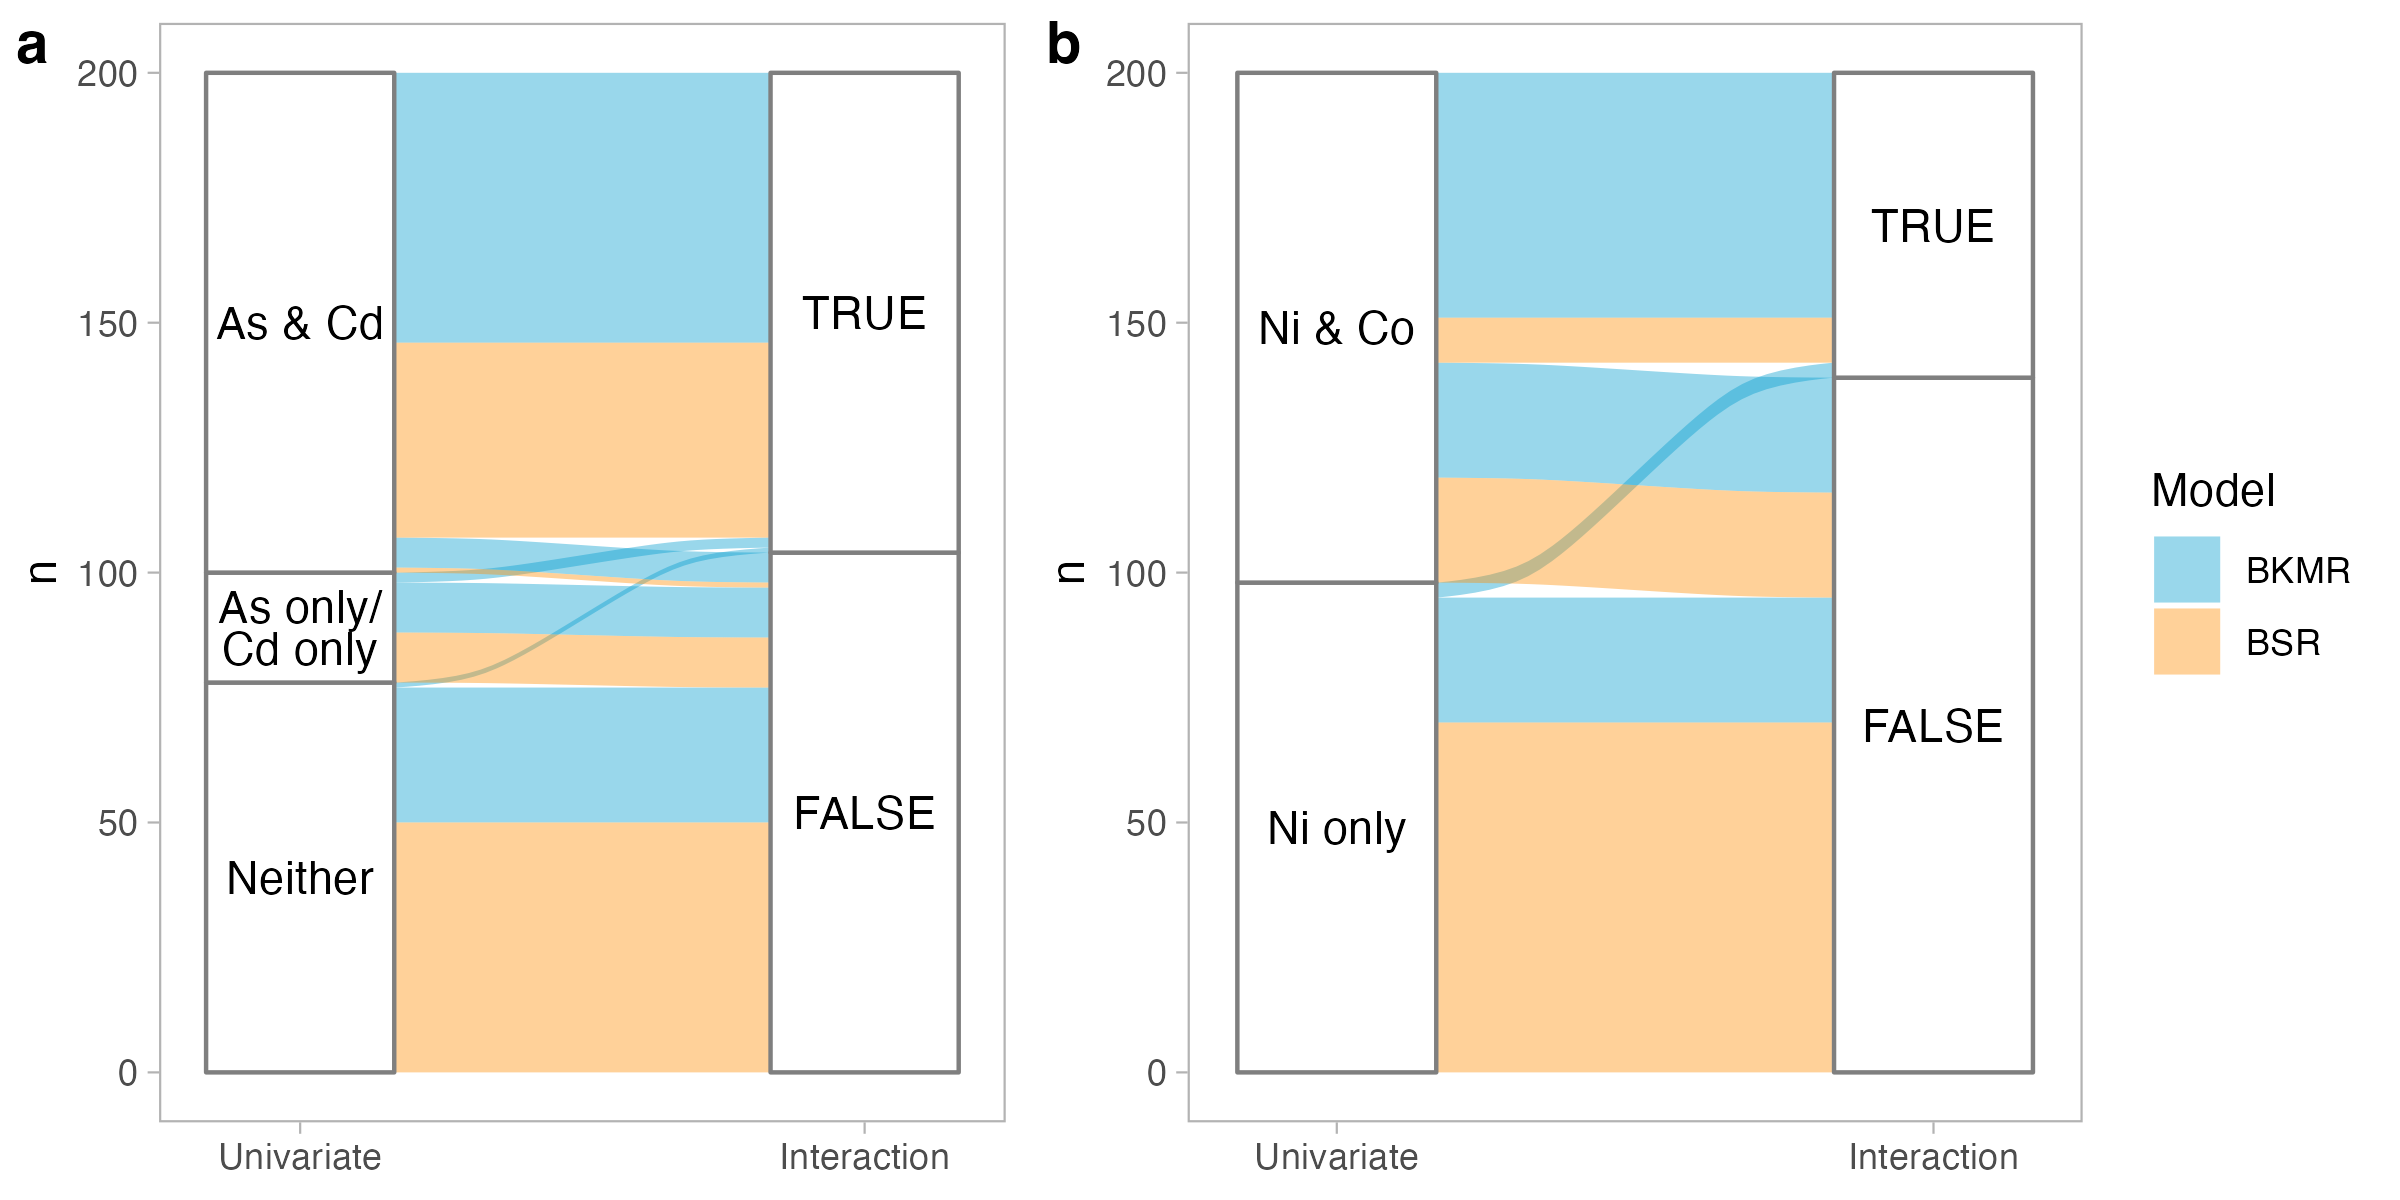
\includegraphics[width=1\linewidth]{figures/ch4_flowchartboth} 

}

\caption{Relationship between detection of the univariate effects of As and Cd (a) and Ni and Co (b) and detection of their interactions. Only cases with a higher effect size, multiplicative interaction in a larger size dataset are included.}\label{fig:flowchart}
\end{figure}
Thus, we suggest that detection of interactions is associated with detection of univariate effects. Interactions between Hg and Ni are easier to detect because they are, themselves, marginally significant. However, interactions between marginally insignificant chemicals are likely to only be detected if the form and effect size of the interaction are such that both chemicals can also be detected marginally. Moreover, it appears that multicollinearity between Ni and Co reduces the ability of BKMR and BSR to detect their interaction.

Next, Table \ref{tab:twowayfdrtab} summarizes the false discovery rate of BKMR and BSR for two-way interactions. Both methods perform well in all scenarios, with false discovery rates below 0.02. This confirms that the above results for sensitivity did not occur by chance. For smaller size datasets, both BKMR and BSR have almost negligible false discovery rates, ranging from 0.0002-0.0025 for BKMR and 0.0009-0.0034 for BSR. In larger size datasets, false discovery rates increase slightly for BKMR, ranging from 0.0016-0.0064. On the other hand, false discovery rates increase notably for BSR in the larger size datasets, ranging from 0.012-0.018. Therefore, false discovery rates for interactions, while still low, should be taken into consideration for BSR with larger sample sizes.
\begin{table}

\caption{\label{tab:twowayfdrtab}False discovery rate of interactions in all scenarios with two-way interactions between exposures.}
\centering
\begin{tabular}[t]{llcccc}
\toprule
\multicolumn{2}{c}{\textbf{ }} & \multicolumn{2}{c}{\textbf{Small (n=252)}} & \multicolumn{2}{c}{\textbf{Large (n=1000)}} \\
\cmidrule(l{3pt}r{3pt}){3-4} \cmidrule(l{3pt}r{3pt}){5-6}
Interaction type & Effect size & BKMR & BSR & BKMR & BSR\\
\midrule
\addlinespace[0.3em]
\multicolumn{6}{l}{\textbf{Hg-Ni}}\\
 & Lower & 0.0011 & 0.0030 & 0.0034 & 0.0125\\

\multirow{-2}{*}{\raggedright\arraybackslash \hspace{1em}Multiplicative} & Higher & 0.0020 & 0.0020 & 0.0048 & 0.0159\\
\addlinespace
 & Lower & 0.0014 & 0.0014 & 0.0034 & 0.0148\\

\multirow{-2}{*}{\raggedright\arraybackslash \hspace{1em}Polynomial} & Higher & 0.0009 & 0.0032 & 0.0064 & 0.0180\\
\addlinespace
\addlinespace[0.3em]
\multicolumn{6}{l}{\textbf{Cd-As}}\\
 & Lower & 0.0011 & 0.0032 & 0.0039 & 0.0123\\

\multirow{-2}{*}{\raggedright\arraybackslash \hspace{1em}Multiplicative} & Higher & 0.0018 & 0.0020 & 0.0059 & 0.0150\\
\addlinespace
 & Lower & 0.0025 & 0.0016 & 0.0036 & 0.0136\\

\multirow{-2}{*}{\raggedright\arraybackslash \hspace{1em}Polynomial} & Higher & 0.0002 & 0.0018 & 0.0034 & 0.0168\\
\addlinespace
\addlinespace[0.3em]
\multicolumn{6}{l}{\textbf{Ni-Co}}\\
 & Lower & 0.0009 & 0.0023 & 0.0025 & 0.0120\\

\multirow{-2}{*}{\raggedright\arraybackslash \hspace{1em}Multiplicative} & Higher & 0.0011 & 0.0009 & 0.0025 & 0.0150\\
\addlinespace
 & Lower & 0.0020 & 0.0034 & 0.0036 & 0.0141\\

\multirow{-2}{*}{\raggedright\arraybackslash \hspace{1em}Polynomial} & Higher & 0.0011 & 0.0030 & 0.0016 & 0.0173\\
\bottomrule
\end{tabular}
\end{table}
In exposure mixture studies, a visual assessment of the estimated exposure-response relationship is often used to characterize the form of a potential interaction, and a common choice for diagnostic plots involves estimating the exposure-response relationship for one chemical at various quantiles of the second (e.g., \protect\hyperlink{ref-howe_prenatal_2020}{Howe et al., 2020}; \protect\hyperlink{ref-valeri_joint_2017}{Valeri et al., 2017}). Figure \ref{fig:hgnibiv} depicts such plots for all scenarios with interactions between Hg and Ni.
\begin{figure}

{\centering 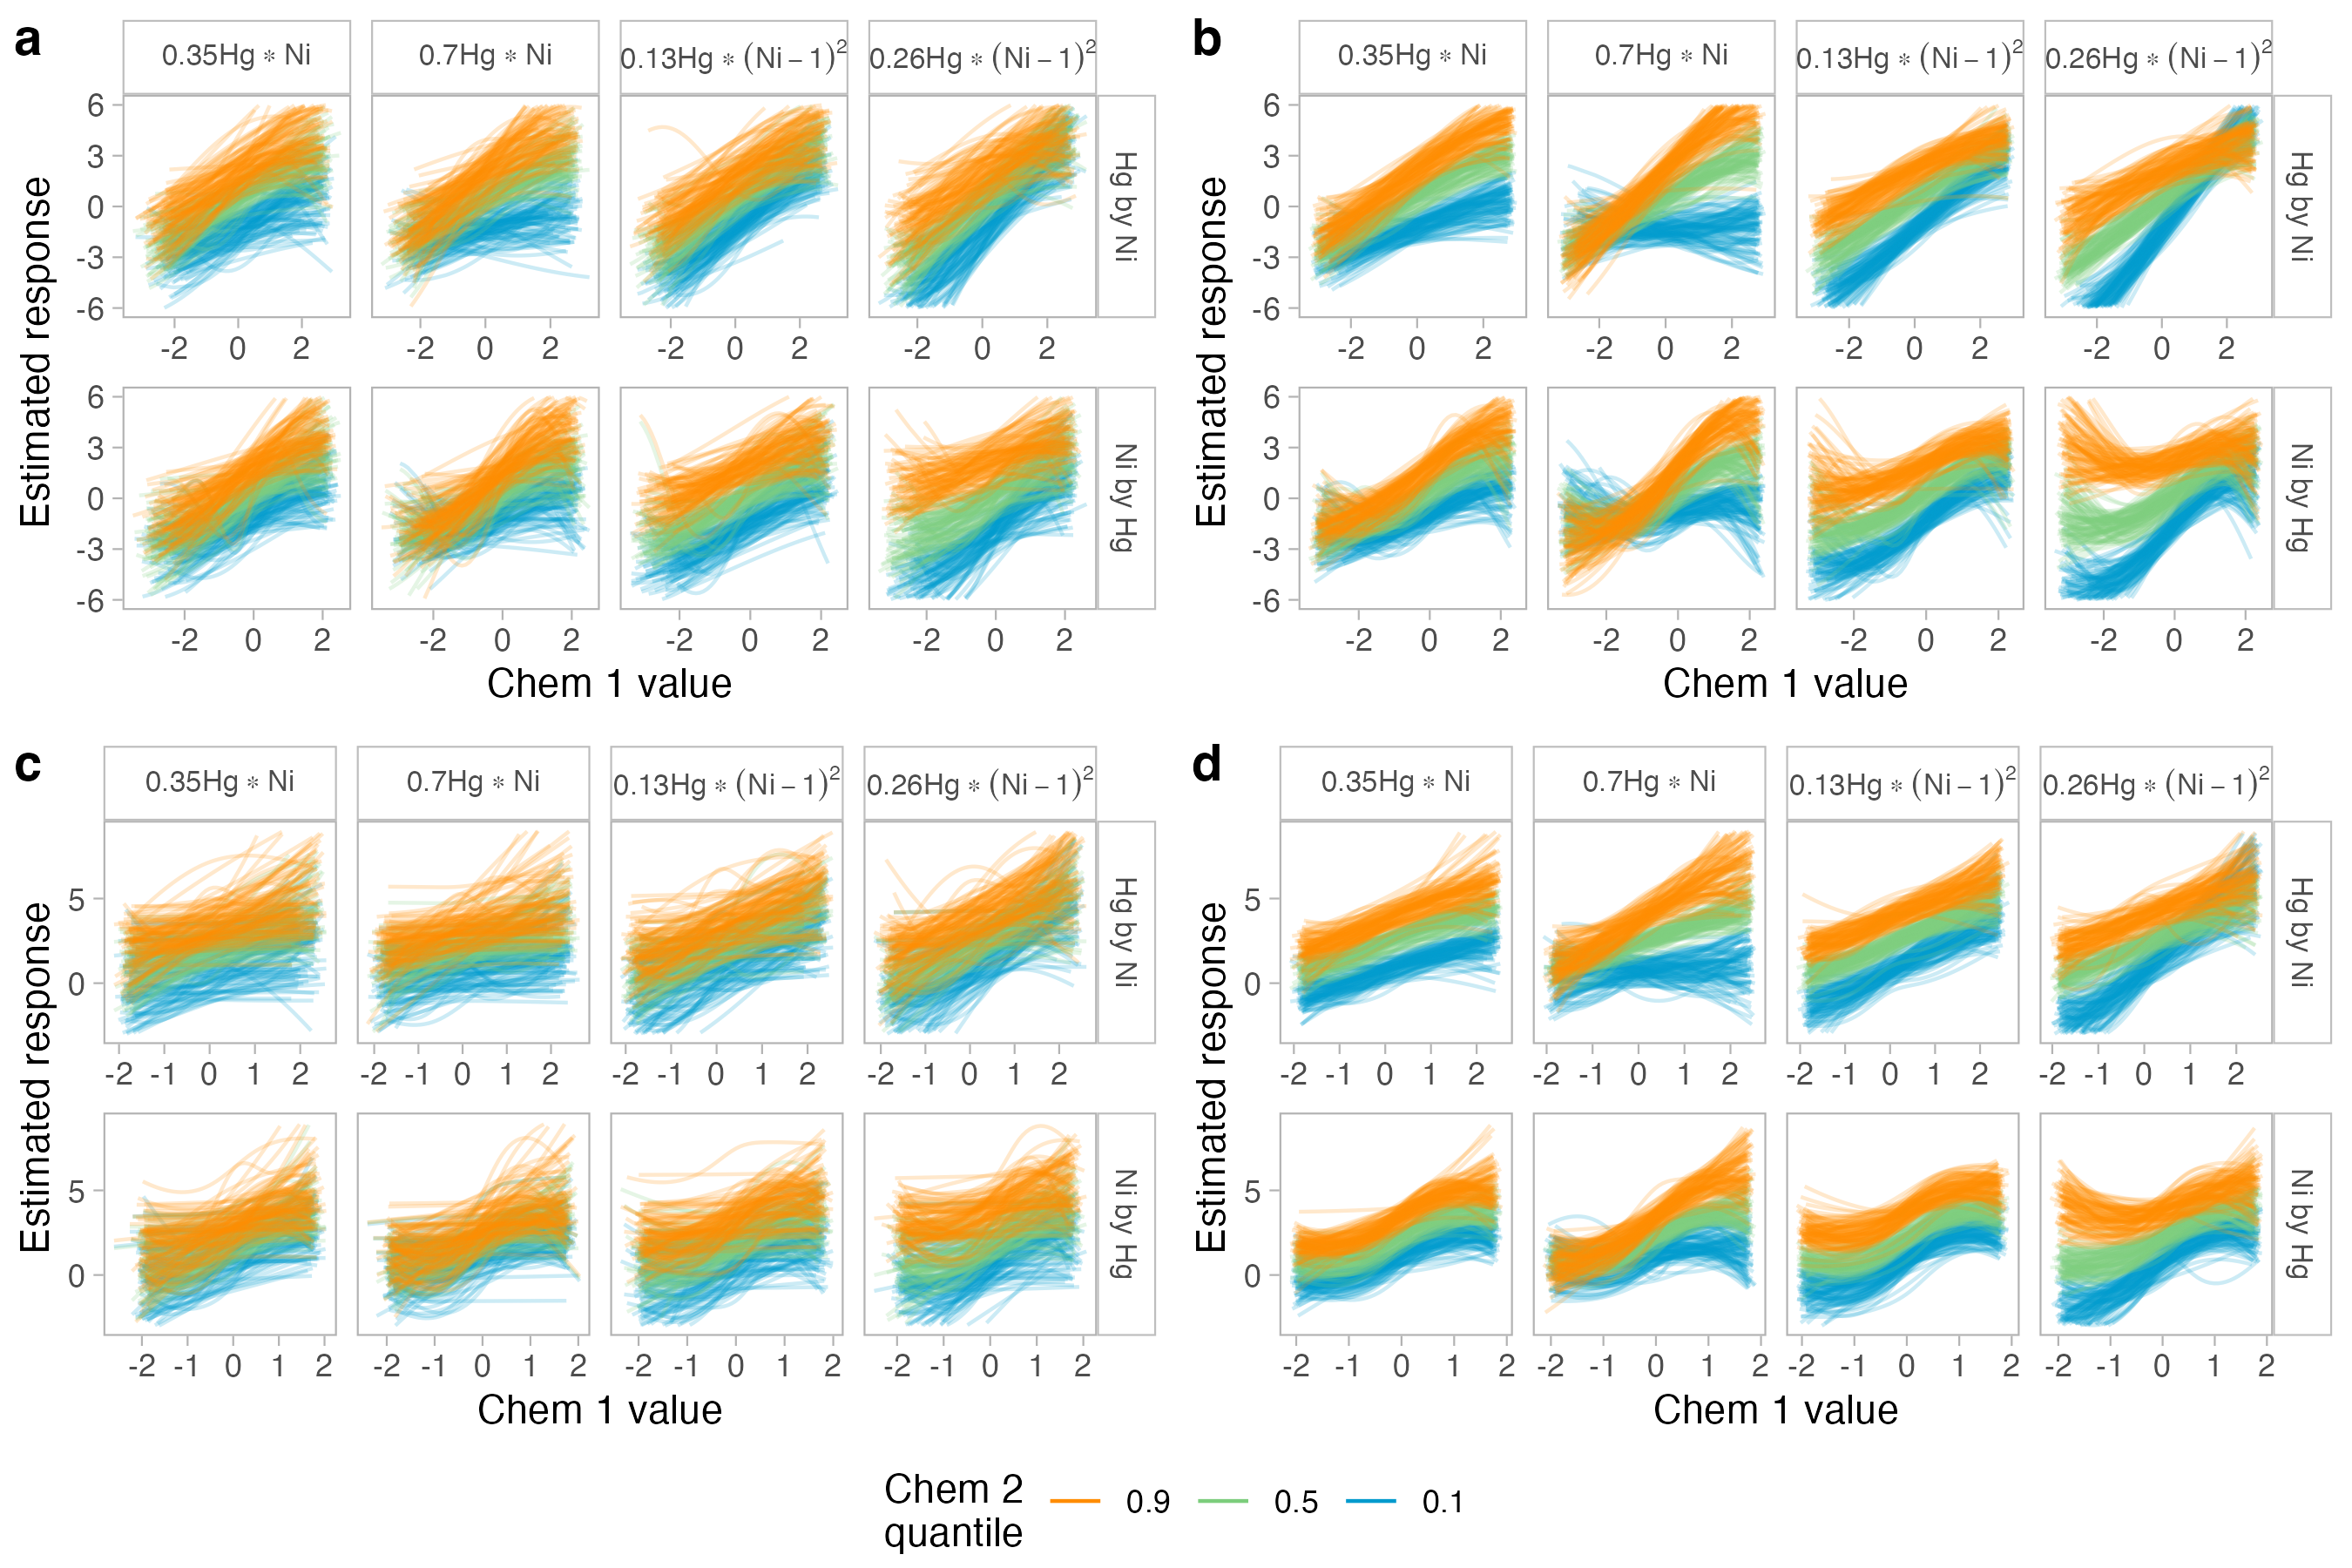
\includegraphics[width=1\linewidth]{figures/ch4_hgni_biv} 

}

\caption{Exposure-response relationships estimated by BKMR in small (a) and large (b) datasets and BSR in small (c) and large (d) datasets, using the first chemical fixed at quantiles of another to assess interactions between Hg and Ni. All other chemicals are fixed at 0.5 quantiles.}\label{fig:hgnibiv}
\end{figure}
The sensitivities in Table \ref{tab:twowaytab} are reflected by the patterns in the diagnostic plots. For instance, the second column of Figures \ref{fig:hgnibiv}b and \ref{fig:hgnibiv}d visualizes the higher effect size, multiplicative interaction between Hg and Ni estimated by BKMR and BSR, respectively. Both models have a sensitivity of 0.76 for this interaction, which is confirmed by the clear difference in the exposure-response relationship between various quantiles of the second chemical. Moreover, the exposure-response relationships are shaped similarly to their associated cross-sections in the 3D theoretical model displayed in Figure \ref{fig:ap2}.

Assessing both directions of the pairwise comparison in these plots (e.g., Hg at quantiles of Ni, as well as Ni at quantiles of Hg) is important as, depending on the true form of the interaction, one direction may have more separation between the estimated relationship at various quantiles. For instance, in the aforementioned example with Hg and Ni, it appears that assessing the relationship between Hg and the health outcome at quantiles of Ni leads to clearer separation than the other way around.

Similar diagnostic plots for all other scenarios, which have similar patterns as those discussed here for Hg and Ni, are shown in Figures \ref{fig:ksmcdas}-\ref{fig:slgnico} in Appendix \ref{suppresults}. In particular, we confirm that the low sensitivities observed in scenarios with interactions between Cd and As, as well as Ni and Co are reflected by estimated exposure-response relationships that do not appear to be associated with interactions. Moreover, it appears that, in Figures \ref{fig:klgcdas} and \ref{fig:klgnico}, the higher effect size, multiplicative interactions between Cd and As and Ni and Co are somewhat captured by BKMR, which reflects their associated sensitivities of 0.57 and 0.52, respectively. Overall, we confirm that patterns in visual diagnostic plots reflect metrics of importance for interactions in both BKMR and BSR.

\hypertarget{three-way-interactions-between-chemicals}{%
\subsection{Three-way interactions between chemicals}\label{three-way-interactions-between-chemicals}}

Next, we discuss the ability of BKMR and BSR to detect three-way interactions between chemicals. Table \ref{tab:threewaysens} summarizes the sensitivity of the oracle MLR, BKMR, and BSR for three-way interactions between Hg, Ni, and Tl. Visual plots of the estimated exposure response relationship for one chemical, while holding the two others in the interaction at their 0.1, 0.5, and 0.9 quantiles, are shown in Figures \ref{fig:ksmtri}-\ref{fig:slgtri}. Due to time constraints, we did not obtain false discovery rates for these interactions.
\begin{table}

\caption{\label{tab:threewaysens}Sensitivity to trivariate interactions between Hg, Ni, and Tl.}
\centering
\begin{tabular}[t]{llrrrrrr}
\toprule
\multicolumn{2}{c}{\textbf{ }} & \multicolumn{3}{c}{\textbf{Small (n=252)}} & \multicolumn{3}{c}{\textbf{Large (n=1000)}} \\
\cmidrule(l{3pt}r{3pt}){3-5} \cmidrule(l{3pt}r{3pt}){6-8}
Interaction type & Effect size & Oracle & BKMR & BSR & Oracle & BKMR & BSR\\
\midrule
 & Lower & 0.19 & 0.00 & 0 & 0.45 & 0.01 & 0.00\\

\multirow{-2}{*}{\raggedright\arraybackslash Multiplicative} & Higher & 0.50 & 0.01 & 0 & 0.97 & 0.00 & 0.01\\
\addlinespace
 & Lower & 0.10 & 0.00 & 0 & 0.48 & 0.00 & 0.00\\

\multirow{-2}{*}{\raggedright\arraybackslash Polynomial} & Higher & 0.49 & 0.00 & 0 & 0.96 & 0.05 & 0.00\\
\bottomrule
\end{tabular}
\end{table}
The oracle MLR sensitivities are similar to the two-way scenarios. As in the case of two-way interactions with marginally insignificant chemicals, BKMR and BSR are generally unable to detect these interactions, with sensitivities ranging from 0-0.05. While Hg and Ni are both marginally significant, Tl is not. Similar to the Ni-Co case, it is difficult to determine whether these patterns are due to inherent difficulties in detecting three-way interactions, or the marginal insignificance of Tl.

\hypertarget{interactions-between-race-and-an-exposure}{%
\subsection{Interactions between race and an exposure}\label{interactions-between-race-and-an-exposure}}

This section includes results for scenarios with an interaction between race, a categorical covariate, and Hg.

Table \ref{tab:reintsens} summarizes the sensitivity of the oracle MLR and BKMR. Note that we were unable to provide formal metrics of importance for interactions from BSR. In total, BKMR failed to converge in either the non-Hispanic white or non-Hispanic other category in 311 out of 400 of the smaller size datasets, which are captured in the ``Uncollapsed'' column of this table. All BKMR models run on datasets with the three smallest race categories, collapsed into one group, converged.
\begin{table}
\begin{threeparttable}
\caption{\label{tab:reintsens}Sensitivity to interactions between the categorical race variable and Hg.}
\centering
\begin{tabular}[t]{llccccc}
\toprule
\multicolumn{2}{c}{\textbf{ }} & \multicolumn{3}{c}{\textbf{Small (n=252)}} & \multicolumn{2}{c}{\textbf{Large (n=1000)}} \\
\cmidrule(l{3pt}r{3pt}){3-5} \cmidrule(l{3pt}r{3pt}){6-7}
\multicolumn{2}{c}{ } & \multicolumn{2}{c}{Uncollapsed} & \multicolumn{1}{c}{Collapsed*} & \multicolumn{2}{c}{ } \\
\cmidrule(l{3pt}r{3pt}){3-4} \cmidrule(l{3pt}r{3pt}){5-5}
Interaction in & Effect size & Oracle & BKMR & BKMR & Oracle & BKMR\\
\midrule
 & Lower & 0.07 & 0.00 & 0.00 & 0.21 & 0.01\\

\multirow{-2}{*}{\raggedright\arraybackslash Original n=27\textsuperscript{\dag}} & Higher & 0.19 & 0.00 & 0.00 & 0.51 & 0.03\\
\addlinespace
 & Lower & 0.12 & 0.00 & 0.00 & 0.39 & 0.03\\

\multirow{-2}{*}{\raggedright\arraybackslash Oirignal n=100\textsuperscript{\ddag}} & Higher & 0.24 & 0.02 & 0.03 & 0.83 & 0.21\\
\bottomrule
\end{tabular}
\begin{tablenotes}
\small
\item [*] "Collapsed" refers to scenarios where the smallest three race categories are collapsed into one stratified model.
\item [\dag] Non-Hispanic black
\item [\ddag] Hispanic born outside US
\end{tablenotes}
\end{threeparttable}
\end{table}
In general, interactions between a categorical variable and a continuous variable are harder to detect. Even in larger datasets where the effect of Hg was doubled in the largest race category (i.e., Hispanic born outside US), the oracle MLR had a sensitivity of 0.83, while BKMR had a much lower sensitivity of 0.21. This is the only scenario in which BKMR's sensitivity exceeded 0.03. Thus, BKMR is generally not able to detect interactions with high sensitivity.

Similar to interactions between chemicals, we can create visual plots of the estimated relationship between Hg and the response within each stratified BKMR and BSR model. Figure \ref{fig:exprespre} displays such plots; in each panel, the estimated relationship in the race category with the interaction is plotted on top, to distinguish it from the other categories.

In some cases, it appears that some degree of interaction is detected by BKMR and BSR. For instance, in the large dataset, when the effect of Hg is increased by 150\% (the lower effect size) in the category Hispanic born outside US, there appears to be some separation in the estimated relationship in that category (shown in red), compared to the other four. However, BKMR's sensitivity in this scenario was only 0.03, indicating that it was under-powered to formally detect this interaction. Based on these plots, it also appears that BSR detects a significant effect from Hg less often than BKMR does, as most of the estimated exposure-response relationships are flatter. This is confirmed in Table \ref{tab:reunivsens}, which displays the sensitivity for Hg in each of the stratified BKMR and BSR model. Thus, BSR is likely more affected by the smaller sample sizes from stratification than BKMR, at least with respect to its univariate metrics of variable importance.
\begin{figure}

{\centering 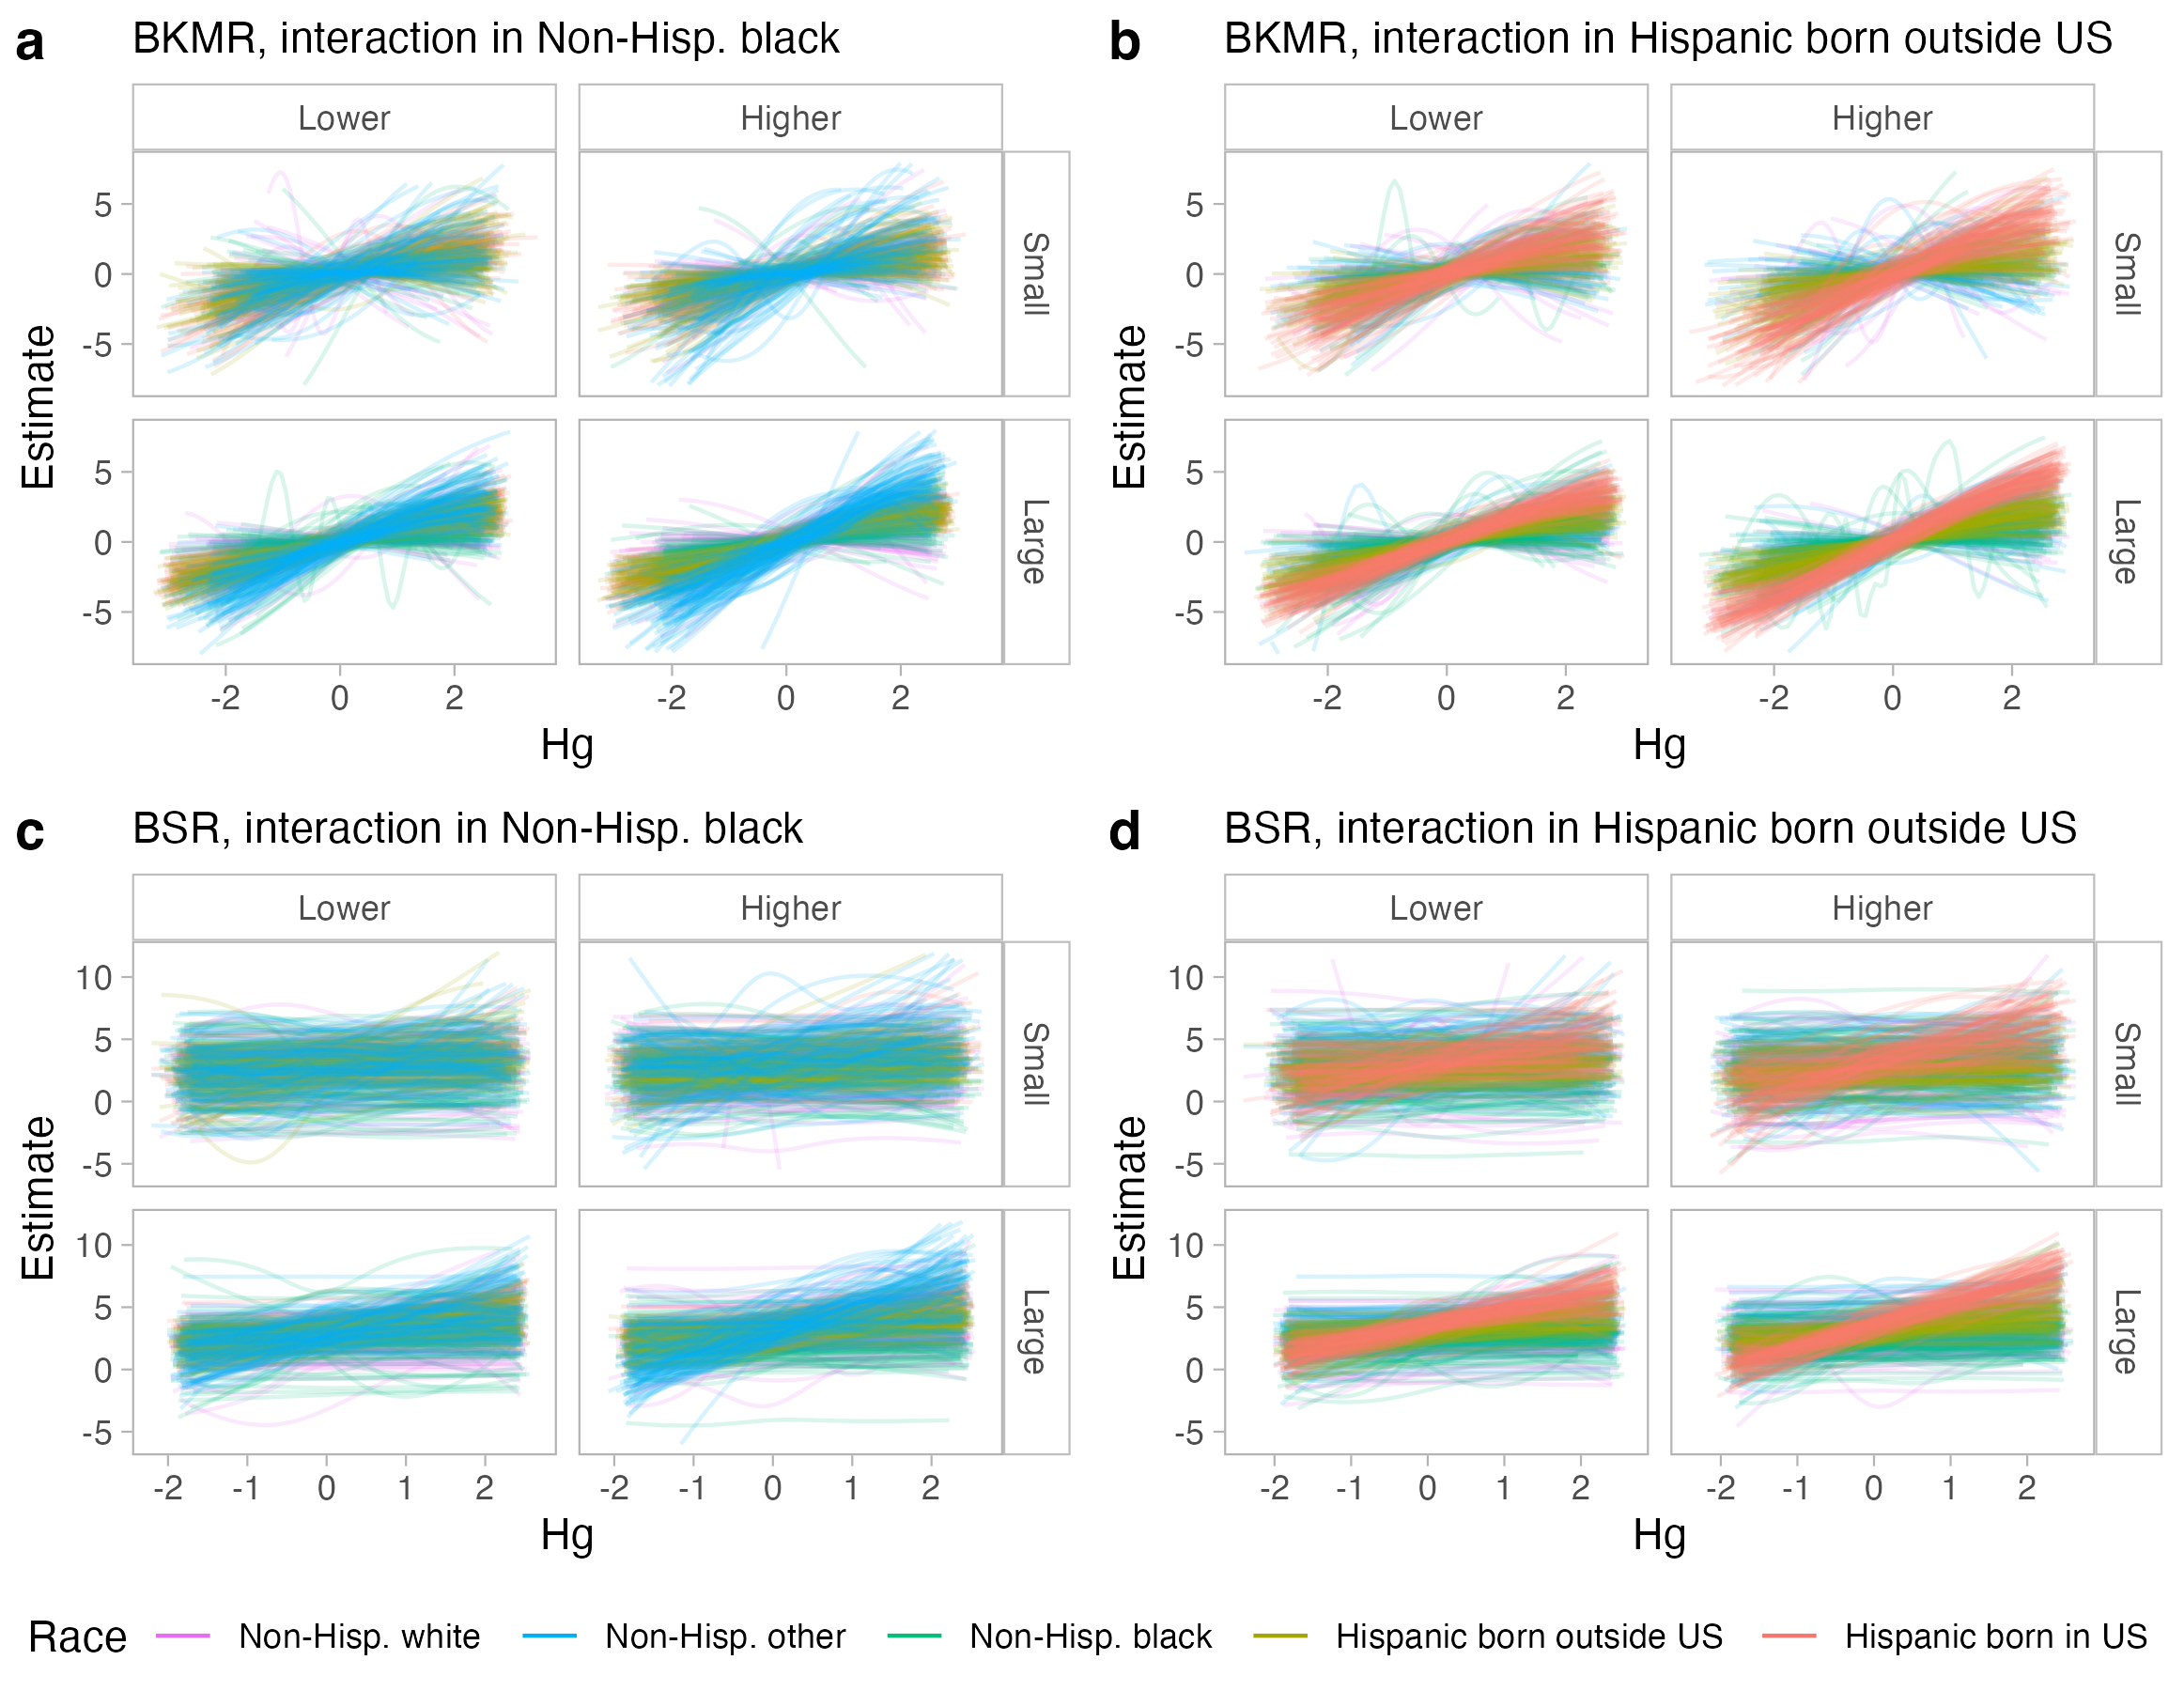
\includegraphics[width=1\linewidth]{figures/ch4_re_expresp} 

}

\caption{Relationship between Hg and response estimated by stratified BKMR and BSR models in smaller and larger datasets. All other chemicals are fixed at 0.5 quantiles. Lower and higher refer to effect sizes, while small and large refer to dataset sizes.}\label{fig:exprespre}
\end{figure}
Therefore, while stratified BKMR and BSR models are, in theory, capable of detecting interactions between a categorical covariate and an exposure, it is difficult to use them for this purpose in practice. The flexibility of BKMR and BSR means that it is not possible to directly conduct inference on the effect sizes of specific chemicals. For BKMR, we are able to construct confidence intervals around the difference of the estimated response at two quantiles of a chemical, and to then compare these confidence intervals between race categories. However, this is a more informal method of inference, as the choice of quantiles is relatively arbitrary. Moreover, for both BKMR and BSR, it is likely that the reduced sample sizes in each stratified model significantly under-power the model for accurately estimating the exposure-response relationship.

Thus, this section highlights the difficulty of using current flexible Bayesian regression methods for detecting interactions between a categorical covariate and a chemical in exposure mixture studies.

\hypertarget{run-time-analysis}{%
\subsection{Run-time analysis}\label{run-time-analysis}}

Finally, we present the run-times for fitting models on the high-performance computing cluster.

Table \ref{tab:runtimes} summarizes the average run-time for each model and sample size, under different interaction scenarios (i.e., various effect sizes and forms of interactions). For model fitting, we used 50,000 MCMC iterations. ``BSR df'' refers to the process for determining the optimal degrees of freedom for the spline regression, while ``BSR mod'' refers to model fitting process. We determined the degrees of freedom in BSR by fitting a grid of four values, each with 1/10 of the MCMC iterations we used for the full model. However, in a full analysis, one should determine the degrees of freedom using the full set of MCMC iterations, so the full run-time for BSR would be approximately four times that reported in the ``BSR mod'' row. We also recall that BKMR was fit using a Gaussian predictive process with 100 knots in the larger size datasets to reduce computational time.

The naive and oracle MLRs take a fraction of a second to run, in both the smaller and larger size datasets, while run-times range from around 15 minutes for BKMR in the smaller size datasets to around 4 hours for BSR (which includes the degrees of freedom selection process) in the larger size datasets. While both Bayesian models are slow, BKMR is still faster than BSR, even when BSR's lengthy degrees of freedom selection process is not factored in. In the smaller size datasets, BKMR takes about 1/6 of the time BSR does, and in the larger size datasets, BKMR takes about 1/2 of the time BSR does. BKMR's speed in comparison to BSR is more pronounced in the smaller size datasets, as BKMR scales with \(n^2\), while BSR scales with \(n\). The Gaussian predictive process likely improves BKMR's speed in the larger size datasets by a wide margin. Moreover, BSR's time may also be attributed to the empirical Baye's strategy for estimating the influential \(\sigma^2_{\boldsymbol\beta}\) parameter, which requires a second set of 50,000 MCMC iterations to run. We also note that BSR appears to take slightly longer in cases with an interaction of higher effect size, compared to the lower effect size, while BKMR's run-time does not appear to be influenced by effect size. Overall, BKMR may be a slightly better choice in settings with smaller datasets, if computational burden is a limiting factor.
\begin{table}

\caption{\label{tab:runtimes}Average run-times in all scenarios with interactions between two or more chemicals, as well as the base case.}
\centering
\begin{tabular}[t]{llccccl}
\toprule
\multicolumn{3}{c}{\textbf{ }} & \multicolumn{2}{c}{\textbf{Multiplicative}} & \multicolumn{2}{c}{\textbf{Polynomial}} \\
\cmidrule(l{3pt}r{3pt}){4-5} \cmidrule(l{3pt}r{3pt}){6-7}
Model & Sample size & Base & Lower & Higher & Lower & Higher\\
\midrule
 & Small & 0.0032 s & 0.0016 s & 0.002 s & 0.0016 s & 0.0017 s\\

\multirow{-2}{*}{\raggedright\arraybackslash Naive} & Large & 0.002 s & 0.002 s & 0.0035 s & 0.0031 s & 0.0025 s\\
\addlinespace
 & Small & 0.0015 s & 0.0015 s & 0.0015 s & 0.0019 s & 0.0016 s\\

\multirow{-2}{*}{\raggedright\arraybackslash Oracle} & Large & 0.0044 s & 0.0018 s & 0.0018 s & 0.0019 s & 0.0024 s\\
\addlinespace
 & Small & 13.56 m & 15.21 m & 15.51 m & 15.20 m & 15.17 m\\

\multirow{-2}{*}{\raggedright\arraybackslash BKMR} & Large & 1.64 h & 1.68 h & 1.62 h & 1.64 h & 1.59 h\\
\addlinespace
 & Small & 30.11 m & 33.15 m & 32.92 m & 33.81 m & 35.11 m\\

\multirow{-2}{*}{\raggedright\arraybackslash BSR df} & Large & 57.22 m & 58.02 m & 1.06 h & 57.75 m & 1.05 h\\
\addlinespace
 & Small & 1.37 h & 1.36 h & 1.42 h & 1.44 h & 1.49 h\\

\multirow{-2}{*}{\raggedright\arraybackslash BSR mod} & Large & 2.92 h & 2.81 h & 3.06 h & 2.87 h & 3.04 h\\
\bottomrule
\end{tabular}
\end{table}
Table \ref{tab:runtimesre} summarizes the average run-times of the naive MLR, oracle MLR, and stratified BKMR in scenarios with an interaction between race and Hg. Again, we note that we were unable to get run-times for BSR within the timeframe of this thesis. However, based on observations of stratified BSR in the high-performance computing cluster, we estimate that it took around 20 hours for all stratified models on one smaller size dataset to run, and 15 hours for one larger size dataset. We suspect that the longer run-time required for smaller size datasets is a result of the MCMC algorithm. We used a Gibbs sampler to fit BSR --- in cases where the model is complex, maintaining reversibility of updates can be computationally challenging (\protect\hyperlink{ref-antonelli_estimating_2020}{Antonelli et al., 2020}).
\begin{table}

\caption{\label{tab:runtimesre}Average run-times in scenarios with an interaction between the categorical race covariate and Hg.}
\centering
\begin{threeparttable}
\begin{tabular}[t]{llcc}
\toprule
Model & Race & Small (n=250) & Large (n=1000)\\
\midrule
Naive & - & 0.0021 s & 0.0035 s\\
\addlinespace
Oracle & - & 0.0019 s & 0.0022 s\\
\addlinespace
 & Non-Hispanic white & 2.50 m & 3.20 m\\

 & Non-Hispanic black & 4.01 m & 4.24 m\\

 & Non-Hispanic other & 1.42 m & 3.34 m\\

 & Hispanic born in US & 5.37 m & 29.24 m\\

 & Hispanic born outside US & 5.65 m & 52.20 m\\

\multirow{-6}{*}{\raggedright\arraybackslash BKMR} & Collapsed non-Hispanic & 4.17 m & -\\
\bottomrule
\end{tabular}
\begin{tablenotes}
\item \textit{Note: } 
\item Original sample sizes of race category: Non-Hispanic white (n=16), Non-Hispanic black (n=27), Non-Hispanic other (n=13), Hispanic born in US (n=87), Hispanic born outside US (n=109), and Collapsed non-Hispanic (n=56=16+27+13).
\end{tablenotes}
\end{threeparttable}
\end{table}
As in the previous case, the MLRs took a fraction of a second to run. The average run-time for BKMR on the smaller size dataset, when added up across all stratified models, is just slightly higher than for the unstratified models. The average run-time for BKMR on the larger size dataset, again added up across all stratified models, is slightly lower than the for the unstratified models. This demonstrates the dependency of BKMR's run-time on \(n^2\), as we did not use a Gaussian predictive process to speed up the stratified models. Finally, based on rough observations of BSR, it was clear that the stratified BSR models took much longer to run than the unstratified BSR models, likely due to challenges with the MCMC algorithm in the reduced sample size. This is a major limitation for using stratified BSR models to detect interactions between a categorical covariate and an exposure.

\hypertarget{discussion}{%
\section{Discussion}\label{discussion}}

Our simulation study provides guidance on the detection and characterization of a wide range of interactions using flexible Bayesian regression models

First, the base case scenario, with no interactions, demonstrates that BKMR and BSR behave as expected. We confirm the results of previous studies, which find that BKMR is able to flexibly capture complex additive exposure-response relationships (i.e., no interactions), though false discovery rates can be higher than other methods (\protect\hyperlink{ref-hoskovec_model_2021}{Hoskovec et al., 2021}; \protect\hyperlink{ref-lazarevic_performance_2020}{Lazarevic et al., 2020}). Similar to Pesenti et al. (\protect\hyperlink{ref-pesenti_comparative_2023}{2023}), we also find that BKMR generally has higher sensitivity than BSR, especially in smaller size datasets.

Next, in cases with interactions between chemicals, we also assessed the univariate signals of chemicals that participated in an interaction. We found that marginally significant chemicals that participated in interactions could occasionally be detected through their univariate effects, depending on the true form of the interaction and if its effect size was large enough. Moreover, the univariate effects of marginally significant chemicals were not detected less often when they participated in an interaction. Together, these results suggest that, at least in the scenarios explored in this simulation, failing to assess for an interaction that would otherwise have been detected should not affect univariate signals, and interactions may sometimes be detected as univariate effects.

Overall, we found that BKMR and BSR did not detect interactions between chemicals as well as the oracle MLR. This suggests that the flexibility afforded by BKMR and BSR leads to drawbacks in sensitivity compared to an ideal (and unrealistic) case, where we know the true form of the interaction. Still, in smaller size datasets with an interaction between chemicals that were themselves marginally significant, BKMR and BSR occasionally detected the signal. And, in larger size datasets, BKMR and BSR produced sensitivities within 0.2-0.3 of the sensitivities produced by the oracle MLR; and, sensitivities for the larger effect sizes of interactions ranged from 0.76 to 0.88, which is relatively reliable.

However, in cases where at least one of the chemicals in the interaction was not marginally significant, BKMR and BSR generally only detected an interaction if there were also significant univariate effects for each chemical. It is typical practice in exposure mixture studies to only search for interactions between chemicals that have significant univariate effects. Thus, we confirm that, for BKMR and BSR, this analytic process should capture most interactions, as interactions between marginally insignificant were rare in our simulations. Moreover, we suggest that multicolllinearity between chemicals reduced sensitivity for interaction. Though, the effects of multicollinearity were difficult to ascertain, as one of the chemicals was marginally insignificant in our simulations. Finally, sensitivity for three-way interactions was very low, though that could also be due to the inclusion of a marginally insignificant chemical in our simulated interactions, rather than inherent challenges with three-way interactions. Additional simulations with multicollinearity and three-way interactions in different scenarios are necessary to verify our results.

Our simulation study extends the findings from Pesenti et al. (\protect\hyperlink{ref-pesenti_comparative_2023}{2023}) by providing more comprehensive guidance for the use of BKMR and BSR for the detection of interactions. Moreover, to our knowledge, this is the first simulation study of interactions in exposure mixtures since the study by Barrera-Gómez et al. (\protect\hyperlink{ref-barrera-gomez_systematic_2017}{2017}). While the methods they considered were only capable of detecting interactions when assuming linearity, the flexible Bayesian regression methods that we considered in our study can incorporate non-linear effects, and can thus be used in a wider range of scenarios.

To our knowledge, this is also the first study to consider interactions between a categorical, sociodemographic covariate and a chemical in an exposure mixture study. Overall, we found that it is very difficult to detect such interactions. First, we were not able to conduct inference on the presence of these interactions using BSR, as we could not find guidance in the literature for constructing confidence intervals on contrasts between values of a continuous predictor in spline regression. Next, for BKMR, interactions were only detected when the overall sample size was 1000 and when the effect of exposure differed in the largest racial/ethnic category. Thus, the detection of such interactions likely requires large sample sizes and sufficient sampling of the group in which the effect of exposure differs compared to the others. This is evidence for oversampling the minority group, as it is often this group that experiences excess effects of exposure due to discriminative social and structural conditions. Lastly, it appeared that the confidence interval approach that we used was under-powered, as there were cases in which there was visual evidence of an interaction in the estimated exposure-response relationship, but BKMR did not produce significant results.

We also briefly comment on run-times. As both BKMR and BSR are Bayesian models that use MCMC algorithms, it is computationally expensive to arrive at a solution. Moreover, BKMR and BSR require prior specifications that can affect the model fit. It would be time-intensive to fit a grid of prior settings in order to assess the impact of, say, the prior on the influential \(r\) parameter in BKMR in order to check the robustness of PIP values. And, running BSR can be especially time intensive on stratified models, as it can become more difficult for the MCMC algorithm to converge in a smaller sample size. Thus, time cost can be a major limitation for model implementation, and it should be taken into consideration particularly when datasets are large, or access to high-performance computing equipment is limited.

\hypertarget{conclusion}{%
\chapter*{Conclusion}\label{conclusion}}
\addcontentsline{toc}{chapter}{Conclusion}

We will continue to encounter novel chemical entities in our day-to-day lives.

Statistical studies of the health risks associated with exposure to chemical pollutants are critical for making modern toxic landscapes more habitable.

As discussed in Chapter \ref{humanistic},

Our simulation study in Chapter \ref{sims} illustrates the challenges of detecting interactions. Still, we were able to achieve high sensitivities using BKMR and BSR to detect interactions between marginally significant chemicals. For

There can be differences in the performance of BKMR and BSR, but neither consistently outperforms the other. Thus, as BKMR is generally more reliable for univariate effects, and also computationally less intensive, we recommend BKMR for

We conclude that BKMR and BSR were generally comparable for detecting interactions between chemicals, as neither consistently outperformed the other in sensitivity for interactions. For the future study of interactions in exposure mixture studies, we recommend using BKMR first to identify both univariate effects and potential interactions with visual diagnostic plots. Then, we recommend using BSR to verify these results, as it tends to have lower false discovery rates for univariate effects and also provides a more formal framework of inference for interactions. As most interactions were only detected when the chemicals were also univariately significant, limiting the search for interactions to those chemicals with univariate PIPs greater than 0.5 should generally be sufficient.
\begin{itemize}
\tightlist
\item
  minority group often experiences social effects of stress. important to oversample the minority group
\end{itemize}
This thesis summarizes the current capabilities of modern Bayesian statistical methods for characterizing complex interactions in exposure mixture studies. In particular, we highlight that such methods are under-powered for detecting potential interactions between

Future work\ldots{}
\begin{itemize}
\tightlist
\item
  analyses would be improved if three-way fdr's were included and BSR run-times recorded, fdr's for race exp
\item
  going forward, change design of simulations study should try three-way interactions and multicollinearity on cases where the chemicals themselves are significant
\item
  figure out method of formal inference for BSR
\item
  identify difficulty of detecting interactions between race and exposure
\item
  continue to explore how studies of exposure can best protect the health and well-being of communities who live and experience the effects of toxicity
\item
  see what happens with even more chemicals
\end{itemize}
Progressing toward a study of exposure that considers how bodies are related to the environment and to each other. As blah blah said, something something entanglement. But this is better!

\appendix

\hypertarget{appa}{%
\chapter{Supplemental output}\label{appa}}

This first appendix includes supplemental output for Chapter \ref{sims}.

\hypertarget{suppmethods}{%
\section{Methods}\label{suppmethods}}

Figure \ref{fig:univlines} depicts the exposure-response relationship for univariate exposures included in all models in simulation.
\begin{figure}

{\centering 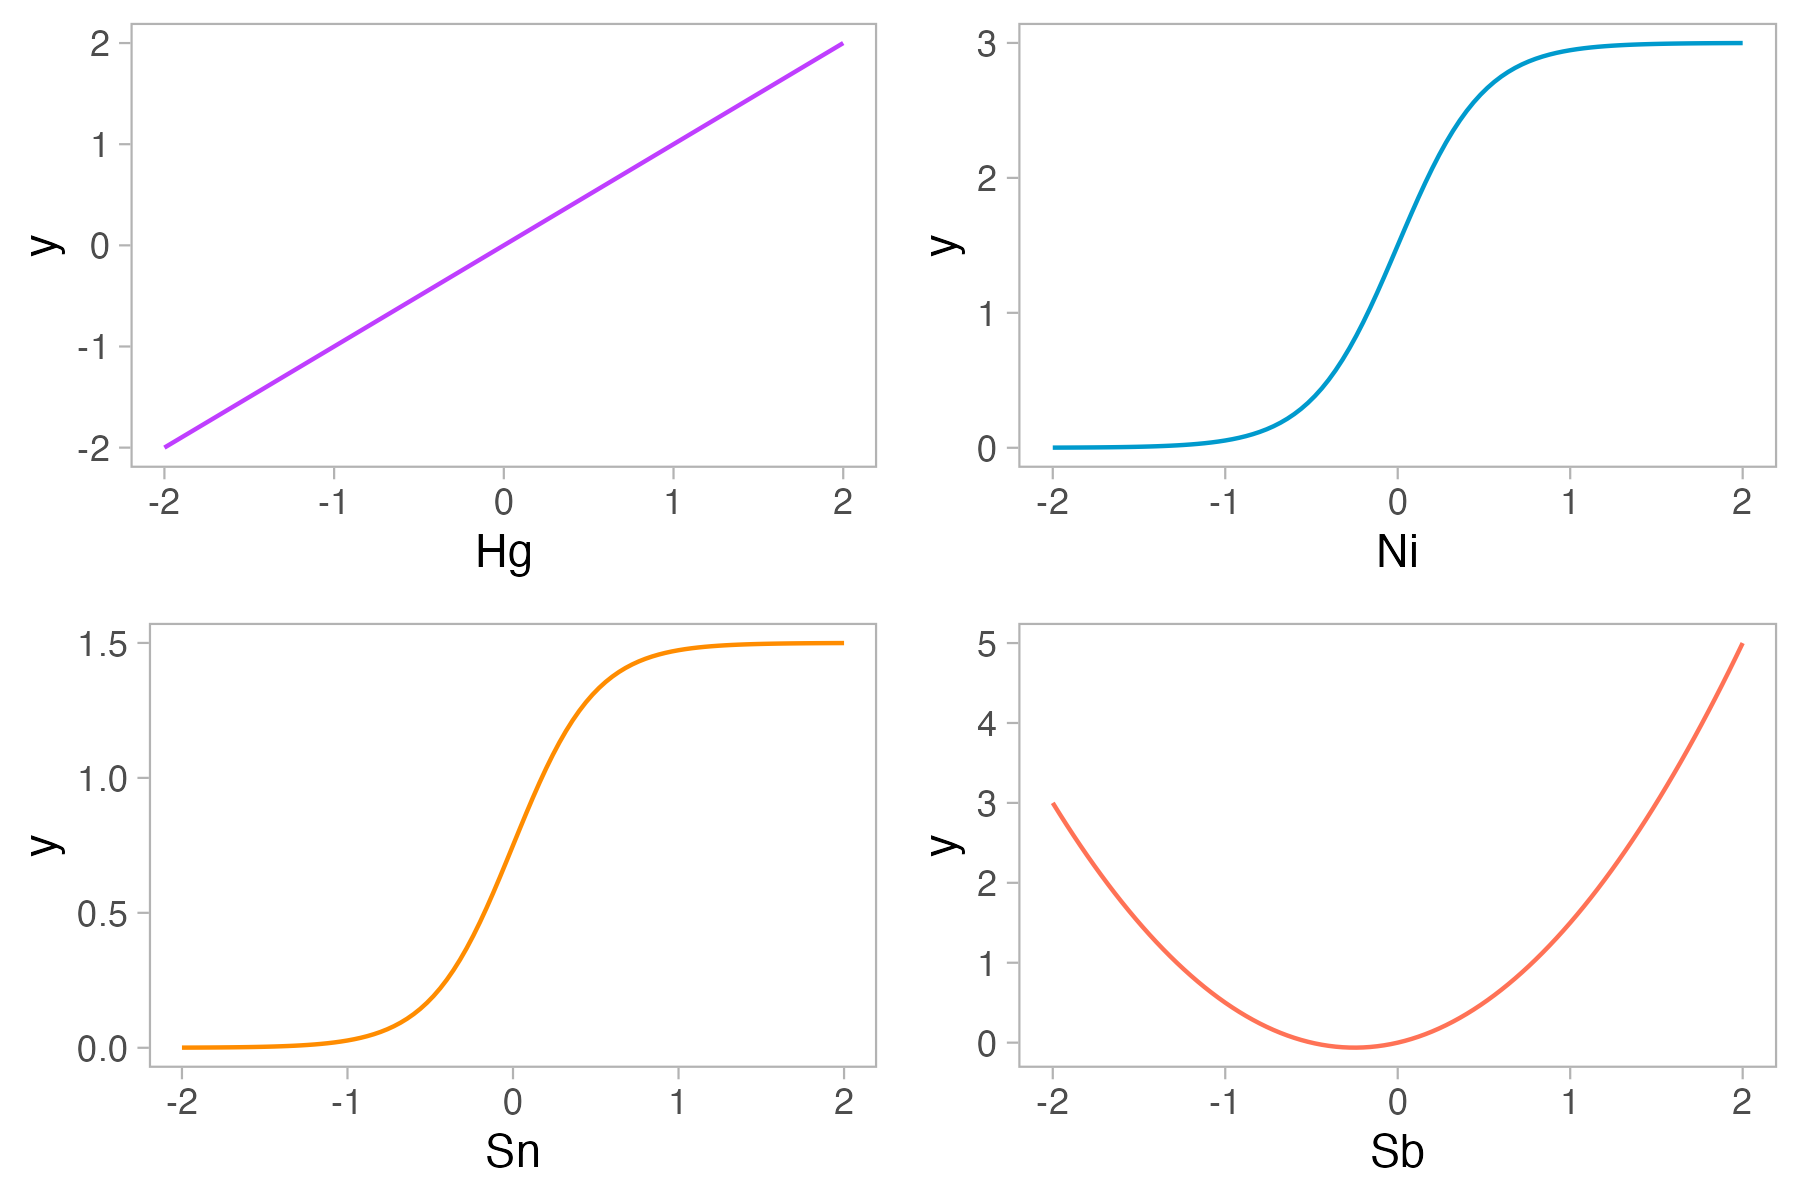
\includegraphics[width=0.75\linewidth]{figures/univariatelines} 

}

\caption{Exposure-response relationship for univariate exposures in all models. Exposure values are log-scaled and then standardized.}\label{fig:univlines}
\end{figure}
Figures \ref{fig:basesurf}-\ref{fig:cp2} depict the exposure-response relationship for all two-way interactions specified in the simulation study.
\begin{figure}

{\centering 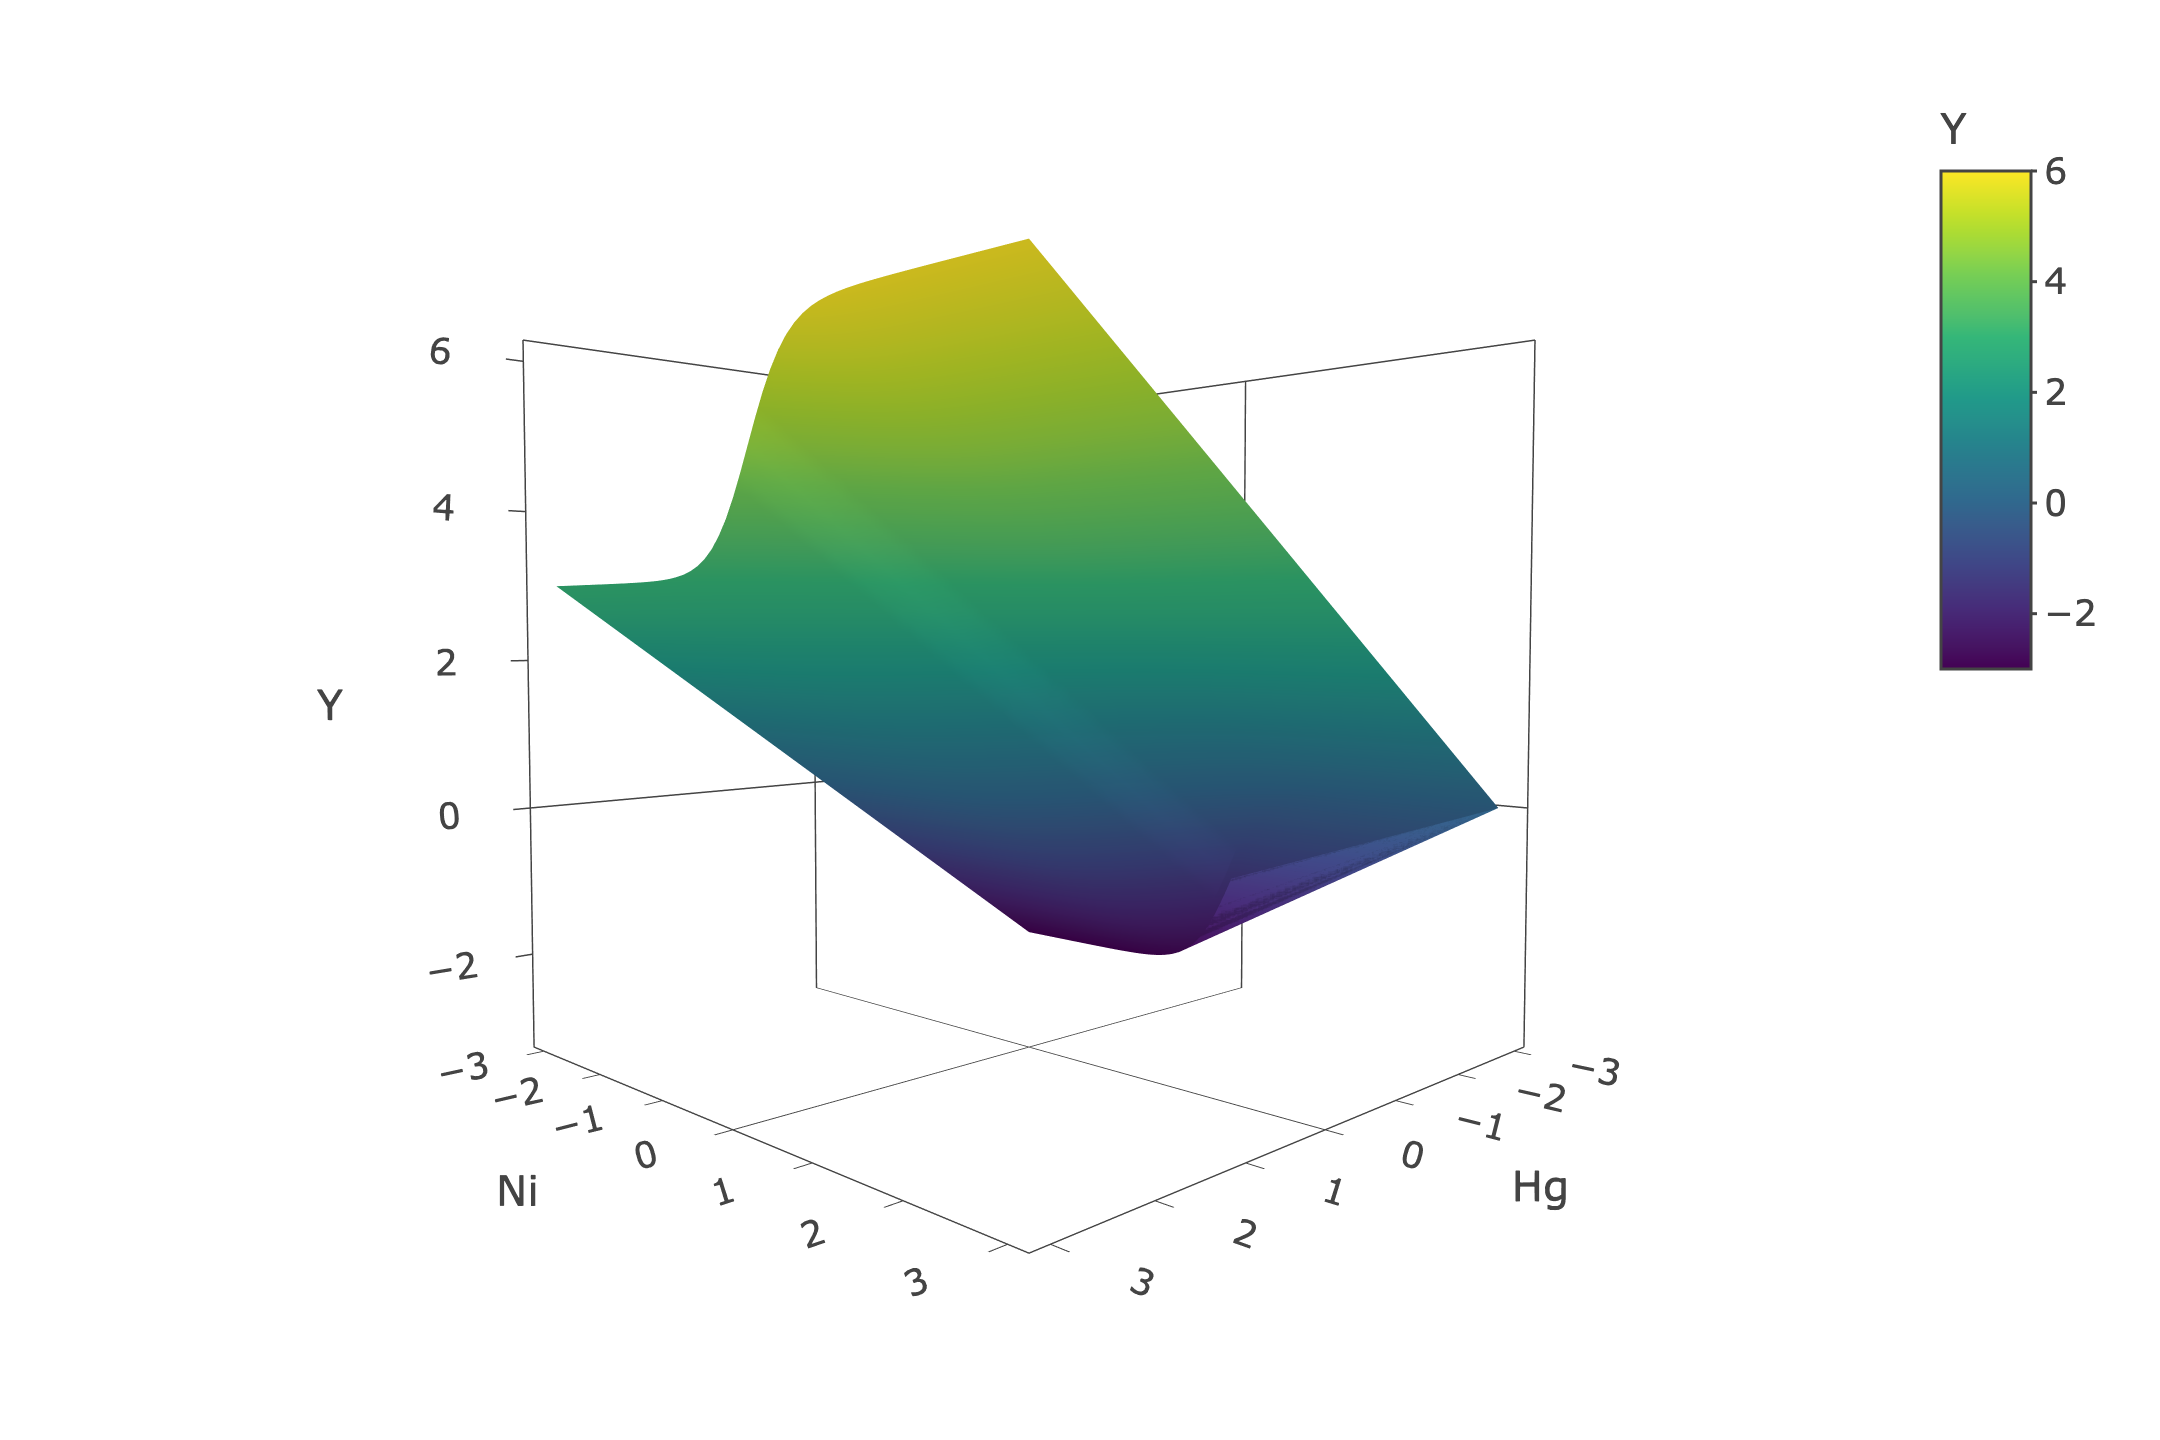
\includegraphics[width=0.5\linewidth]{figures/surfaces/p00} 

}

\caption{Exposure-response surface for base case: $Y=$ Hg $+\frac{3}{1+\textrm{exp}(-4\textrm{Ni})}$.}\label{fig:basesurf}
\end{figure}
\begin{figure}

{\centering 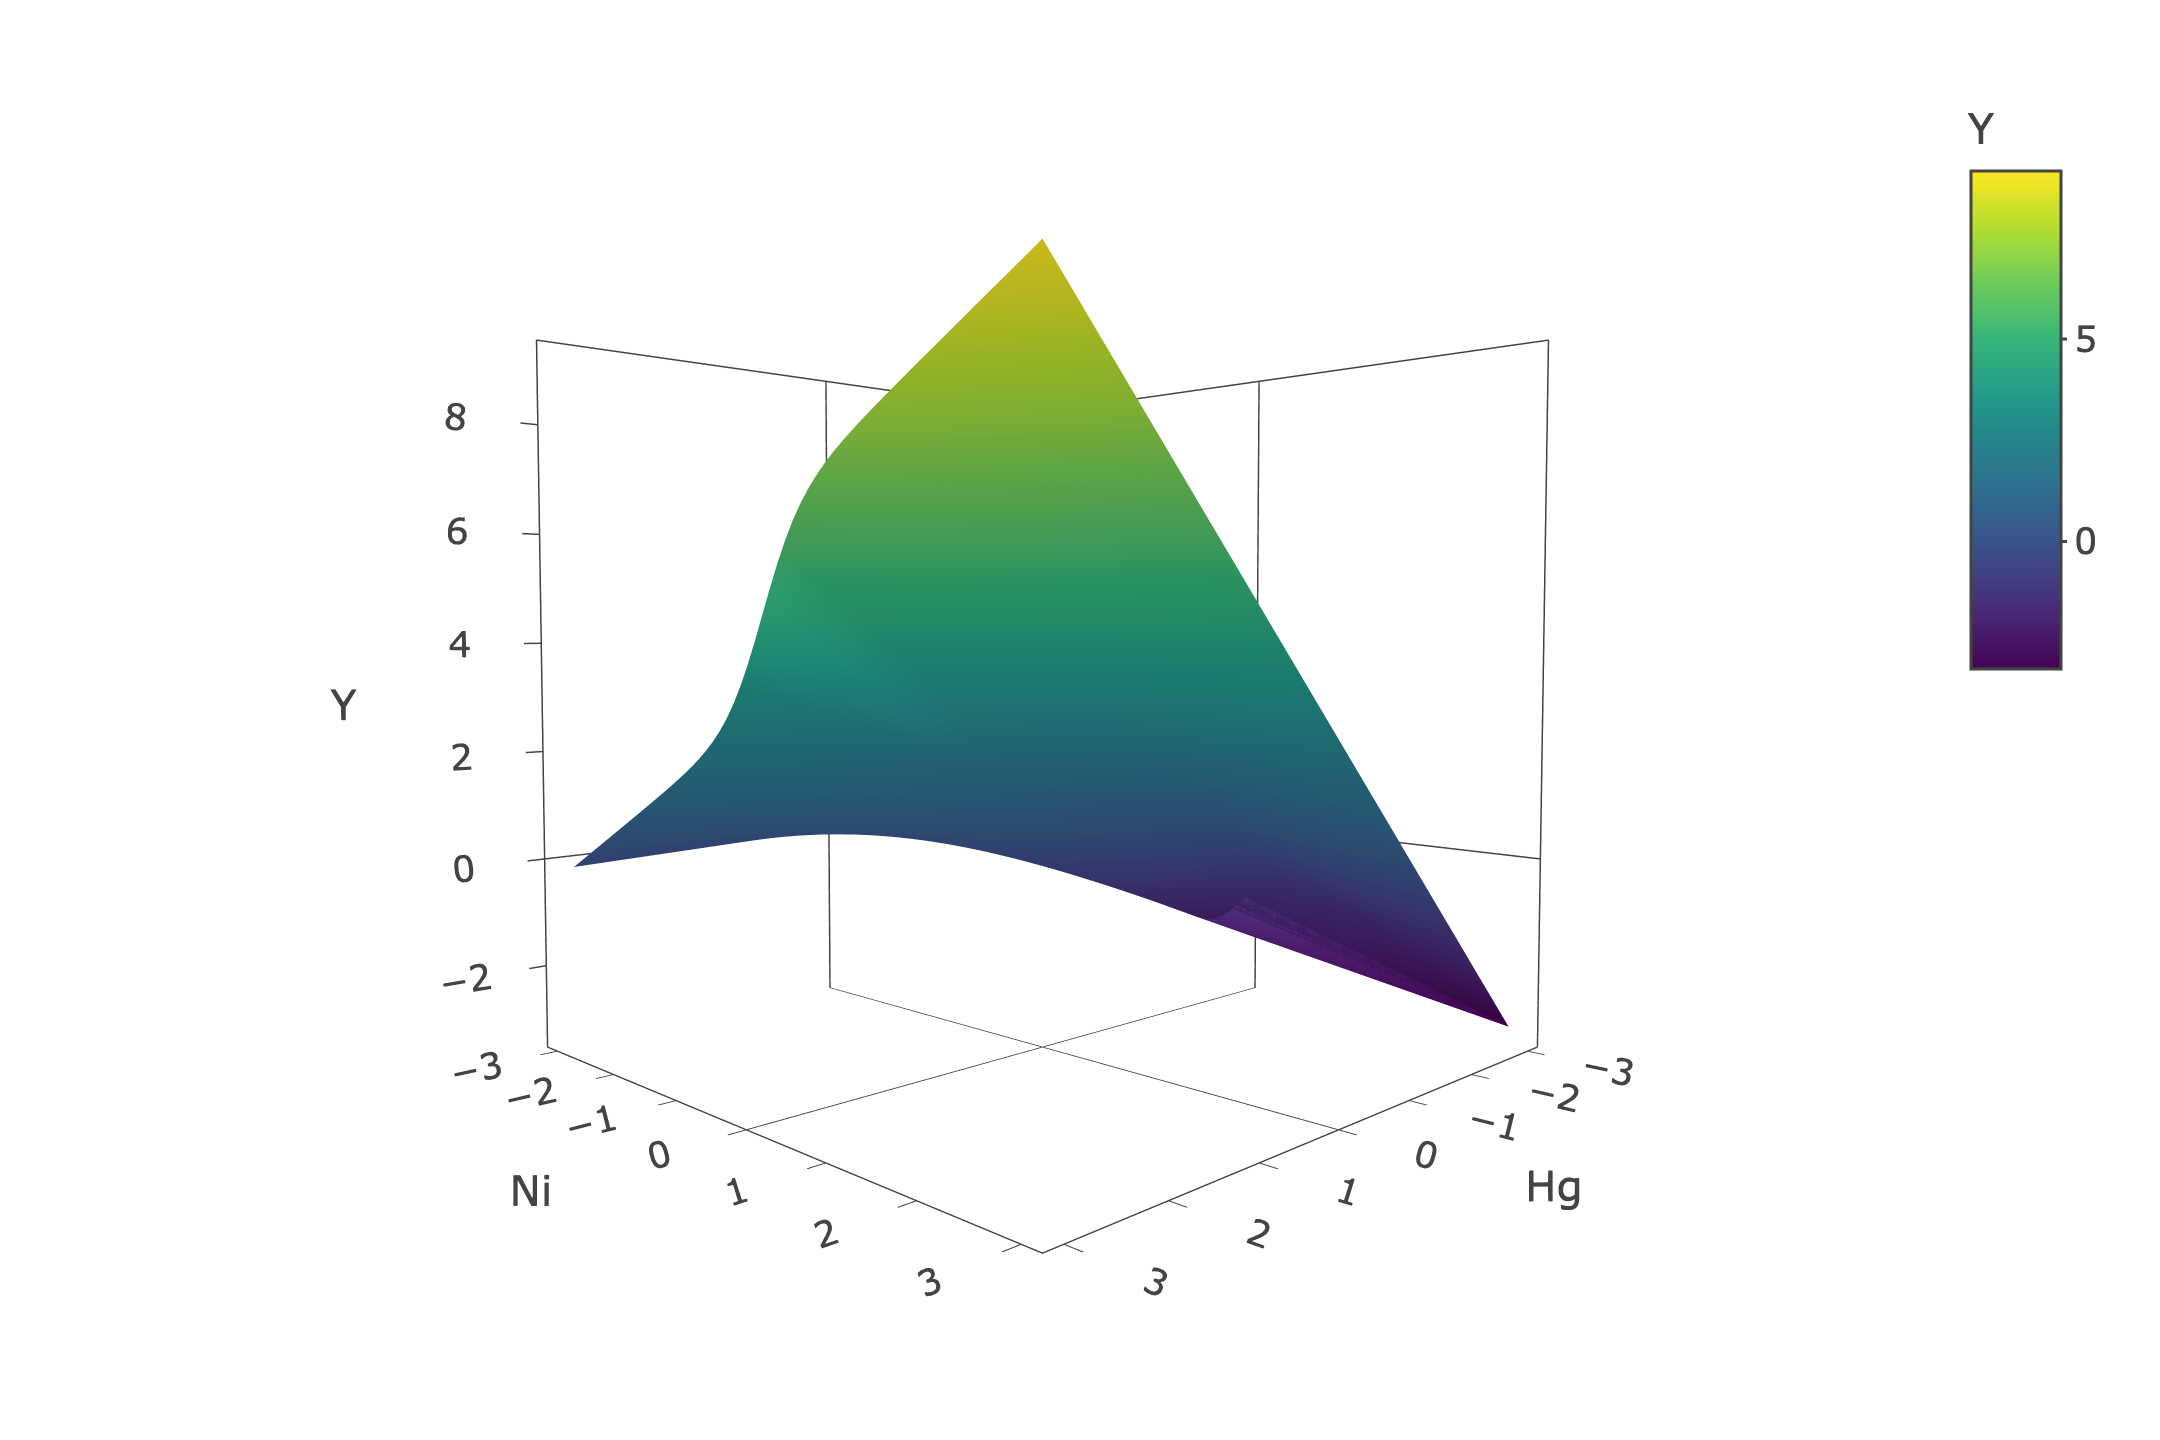
\includegraphics[width=0.5\linewidth]{figures/surfaces/am1} 

}

\caption{Exposure-response surface for a multiplicative interaction between Hg and Ni at the lower effect size: $Y=$ Hg $+\frac{3}{1+\textrm{exp}(-4\textrm{Ni})}$ + 0.35Hg$*$Ni.}\label{fig:am1}
\end{figure}
\begin{figure}

{\centering 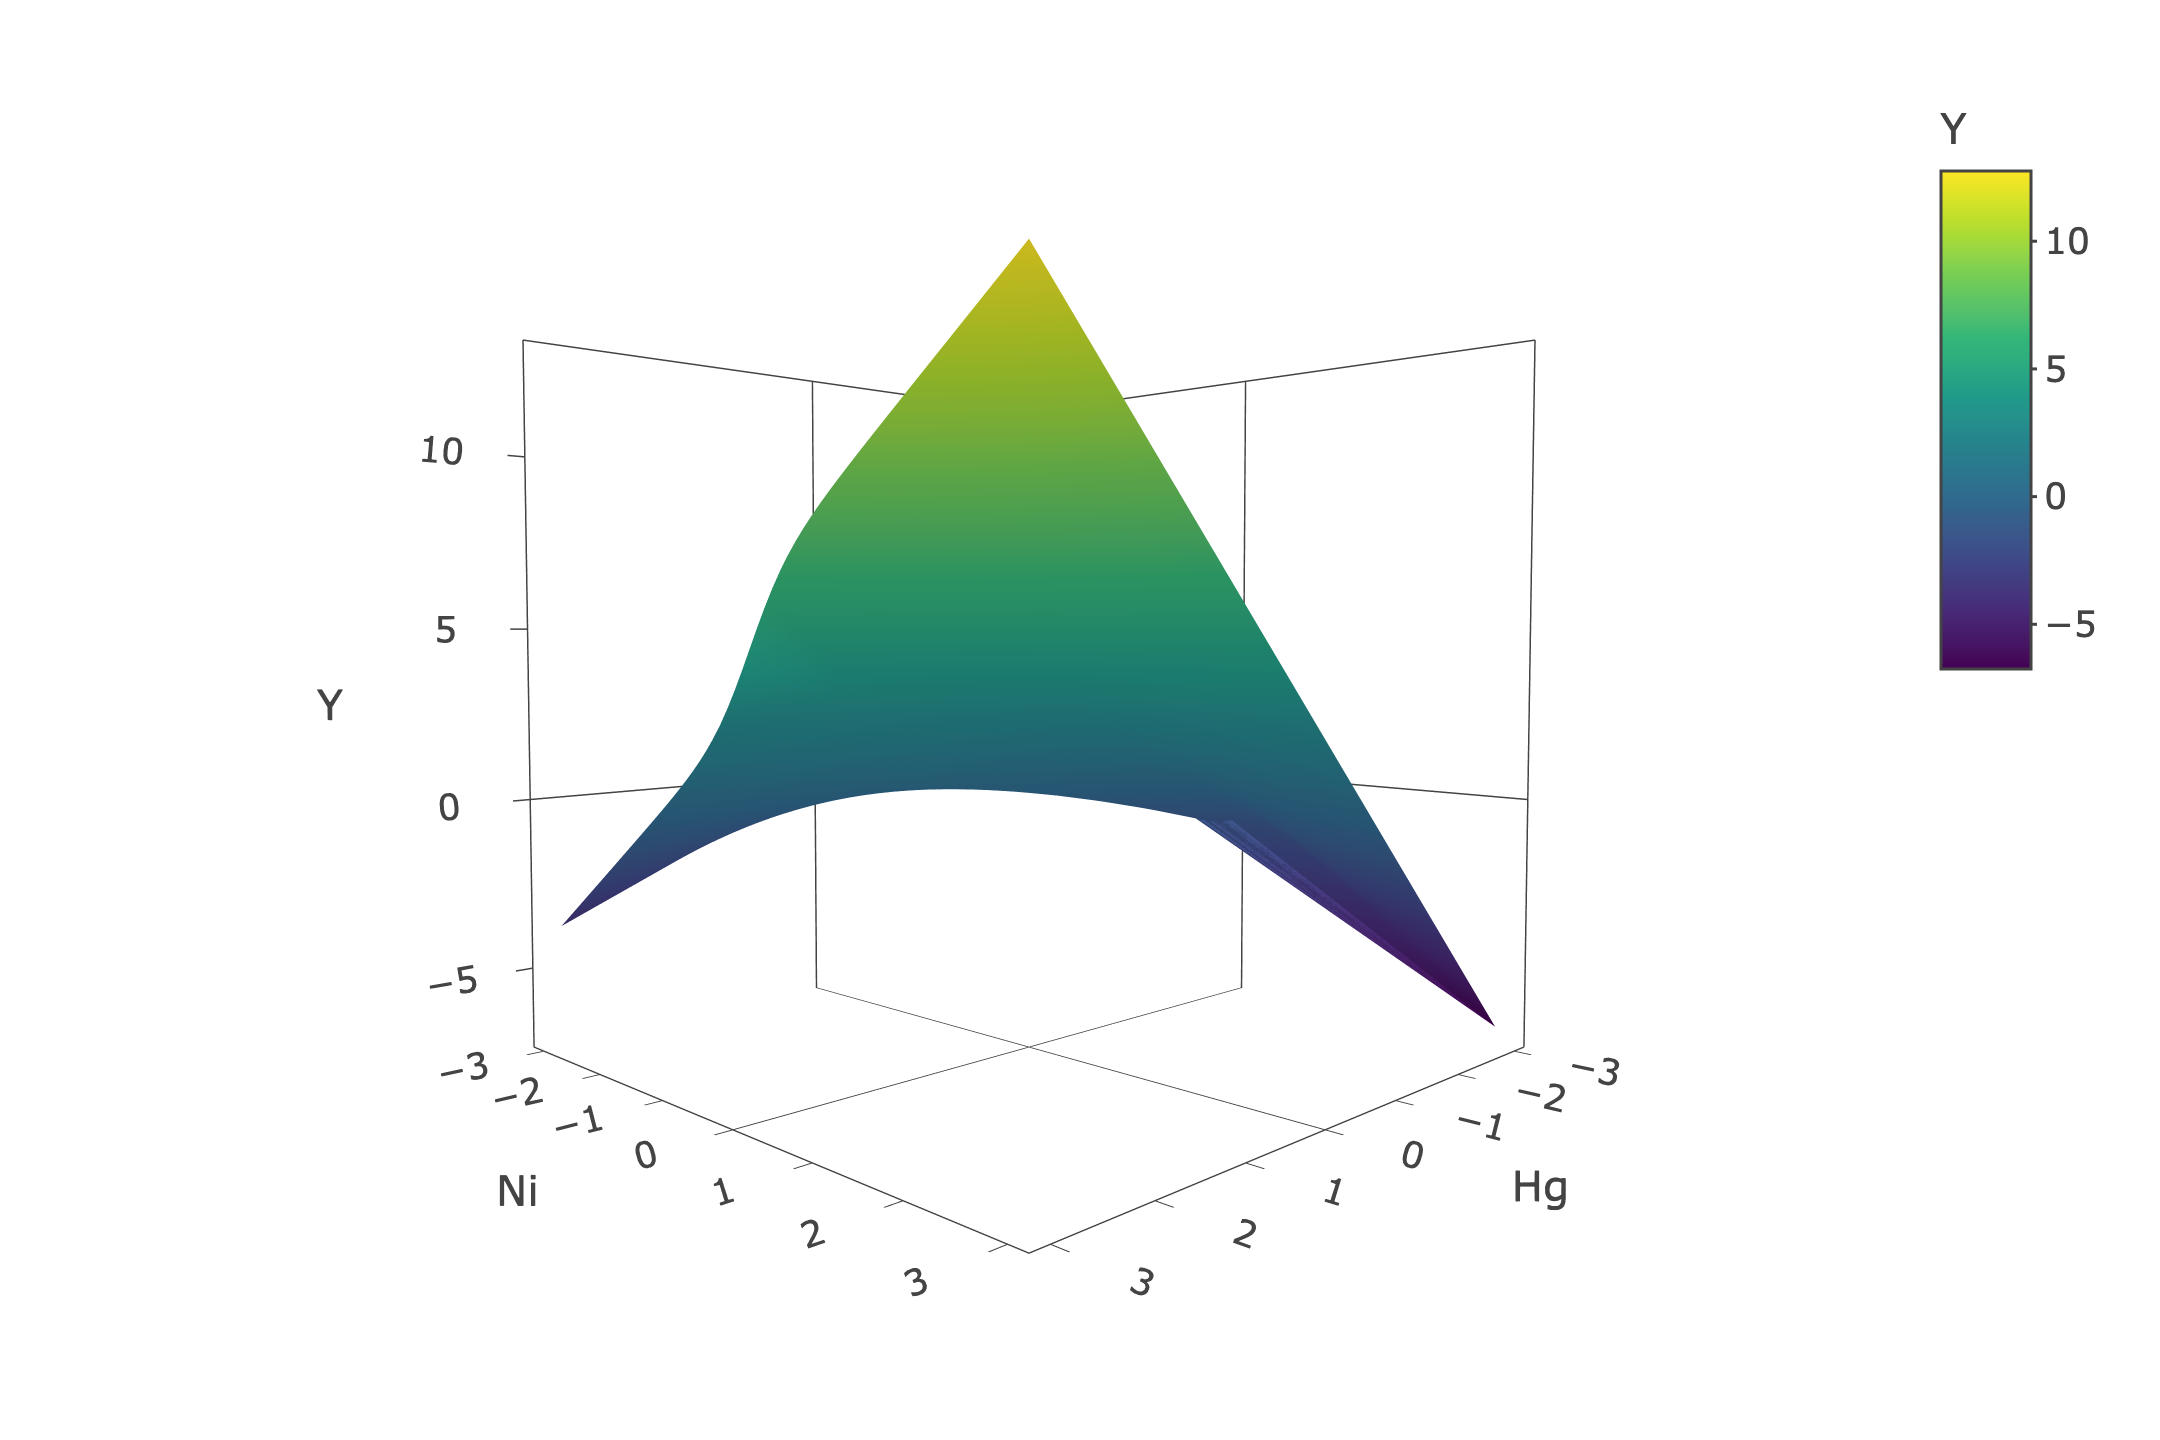
\includegraphics[width=0.5\linewidth]{figures/surfaces/am2} 

}

\caption{Exposure-response surface for a multiplicative interaction between Hg and Ni at the higher effect size: $Y=$ Hg $+\frac{3}{1+\textrm{exp}(-4\textrm{Ni})}$ + 0.7Hg$*$Ni.}\label{fig:am2}
\end{figure}
\begin{figure}

{\centering 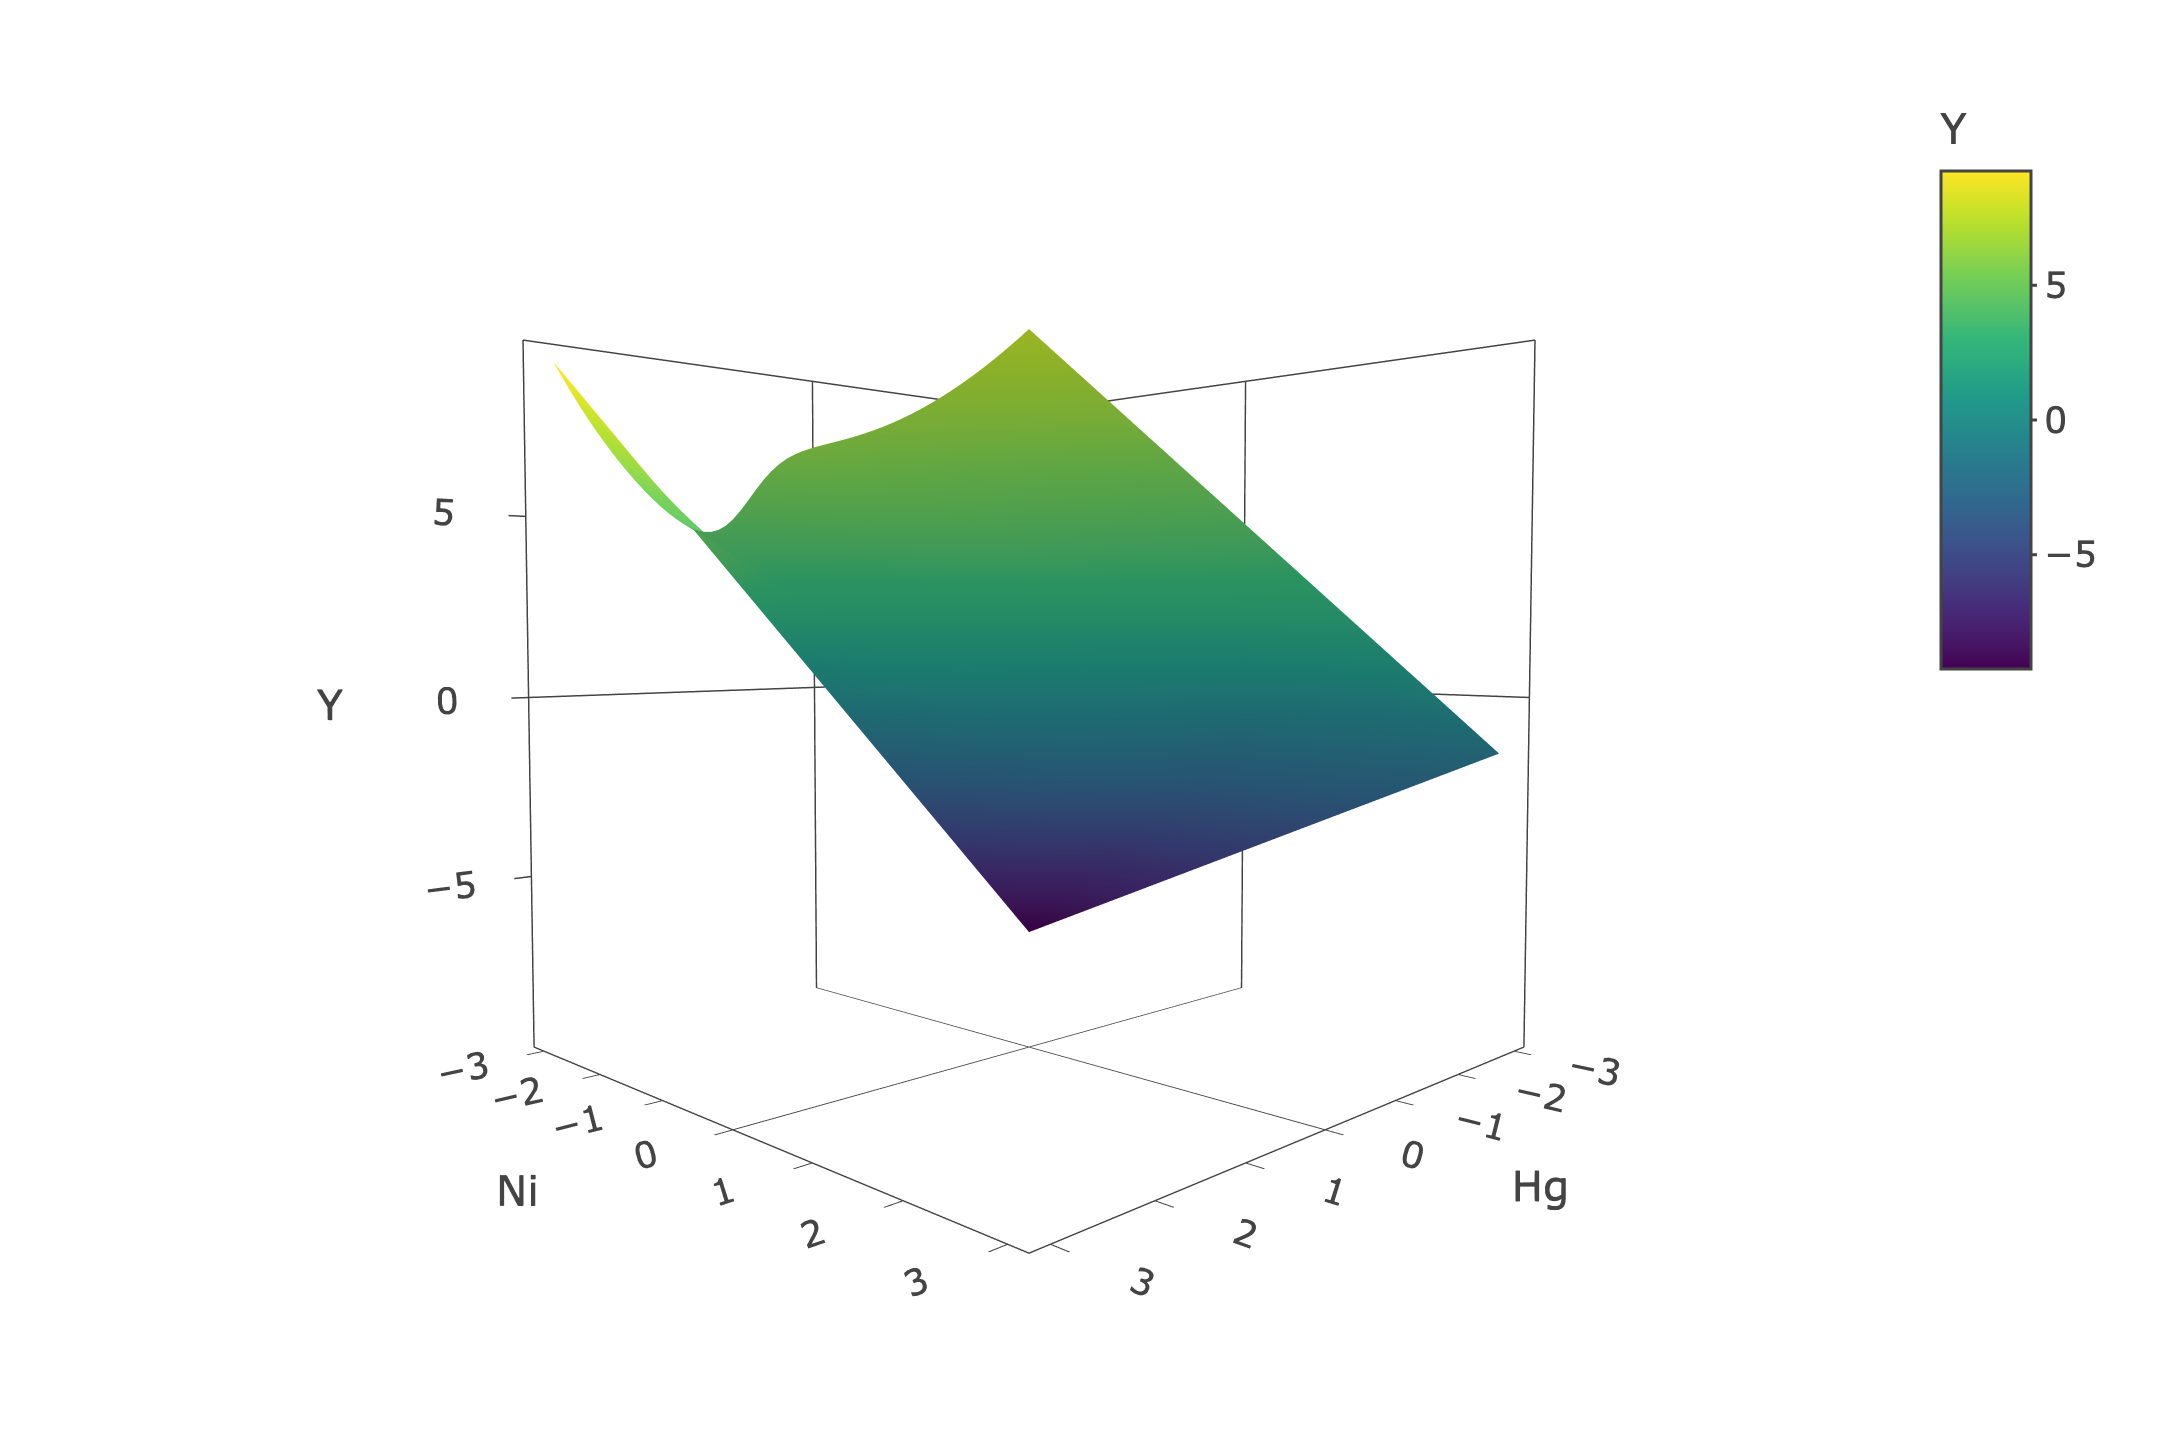
\includegraphics[width=0.5\linewidth]{figures/surfaces/ap1} 

}

\caption{Exposure-response surface for a polynomial interaction between Hg and Ni at the lower effect size: $Y=$ Hg $+\frac{3}{1+\textrm{exp}(-4\textrm{Ni})}$ + 0.3Hg$*($Ni$-1)^2$.}\label{fig:ap1}
\end{figure}
\begin{figure}

{\centering 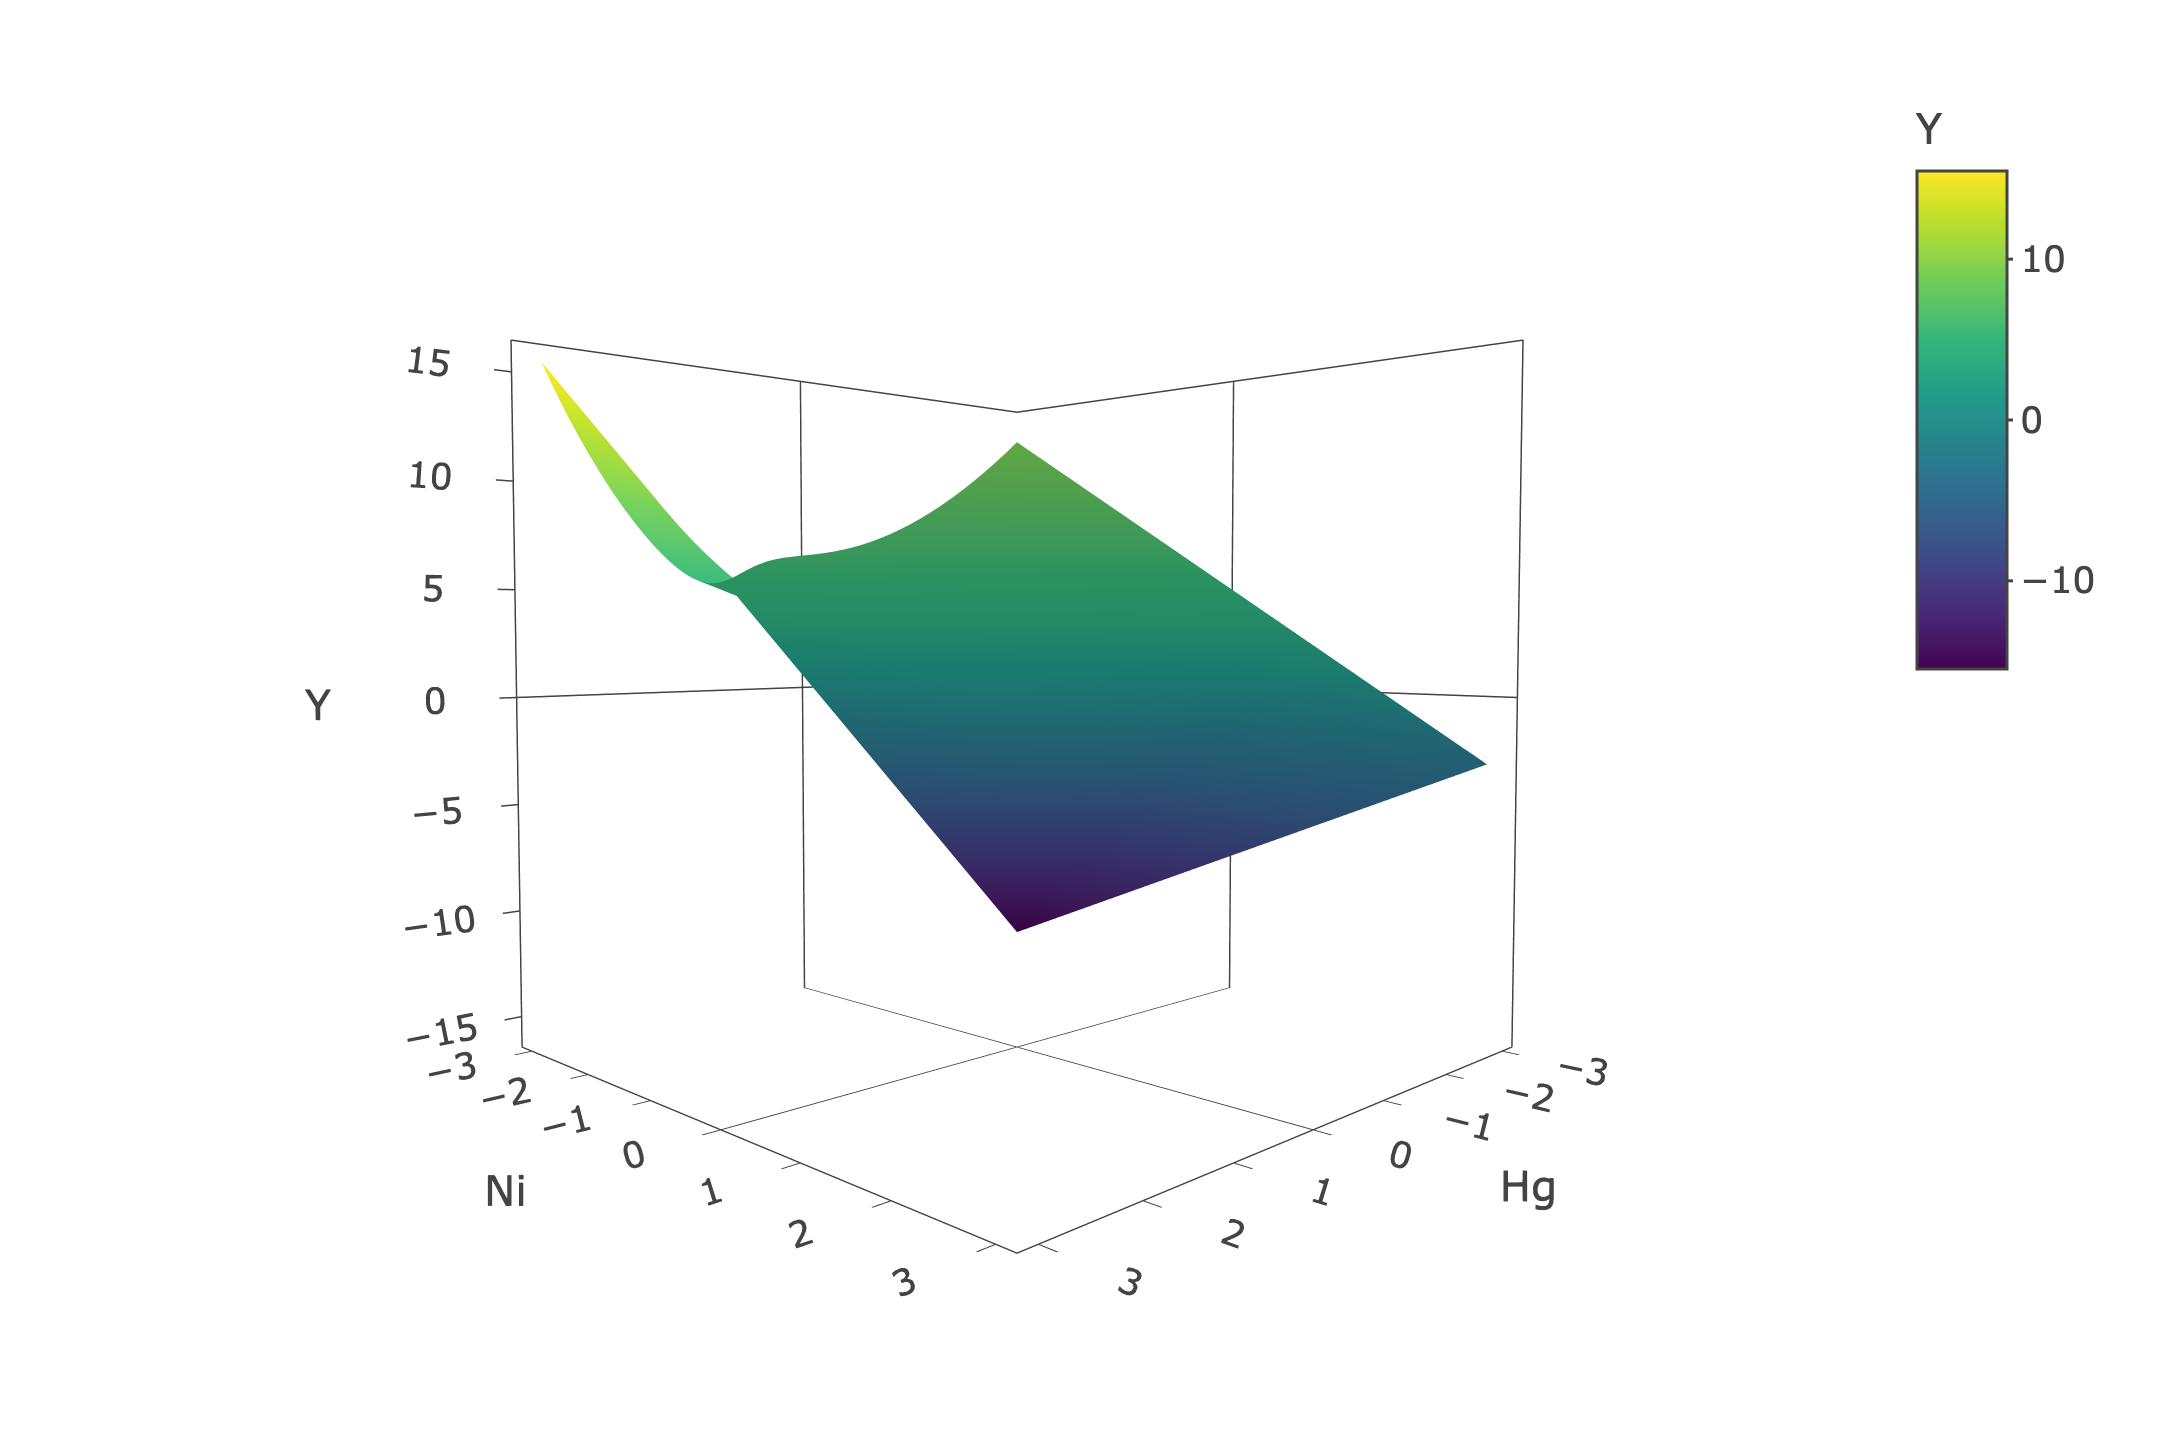
\includegraphics[width=0.5\linewidth]{figures/surfaces/ap2} 

}

\caption{Exposure-response surface for a polynomial interaction between Hg and Ni at the higher effect size: $Y=$ Hg $+\frac{3}{1+\textrm{exp}(-4\textrm{Ni})}$ + 0.6Hg$*($Ni$-1)^2$.}\label{fig:ap2}
\end{figure}
\begin{figure}

{\centering 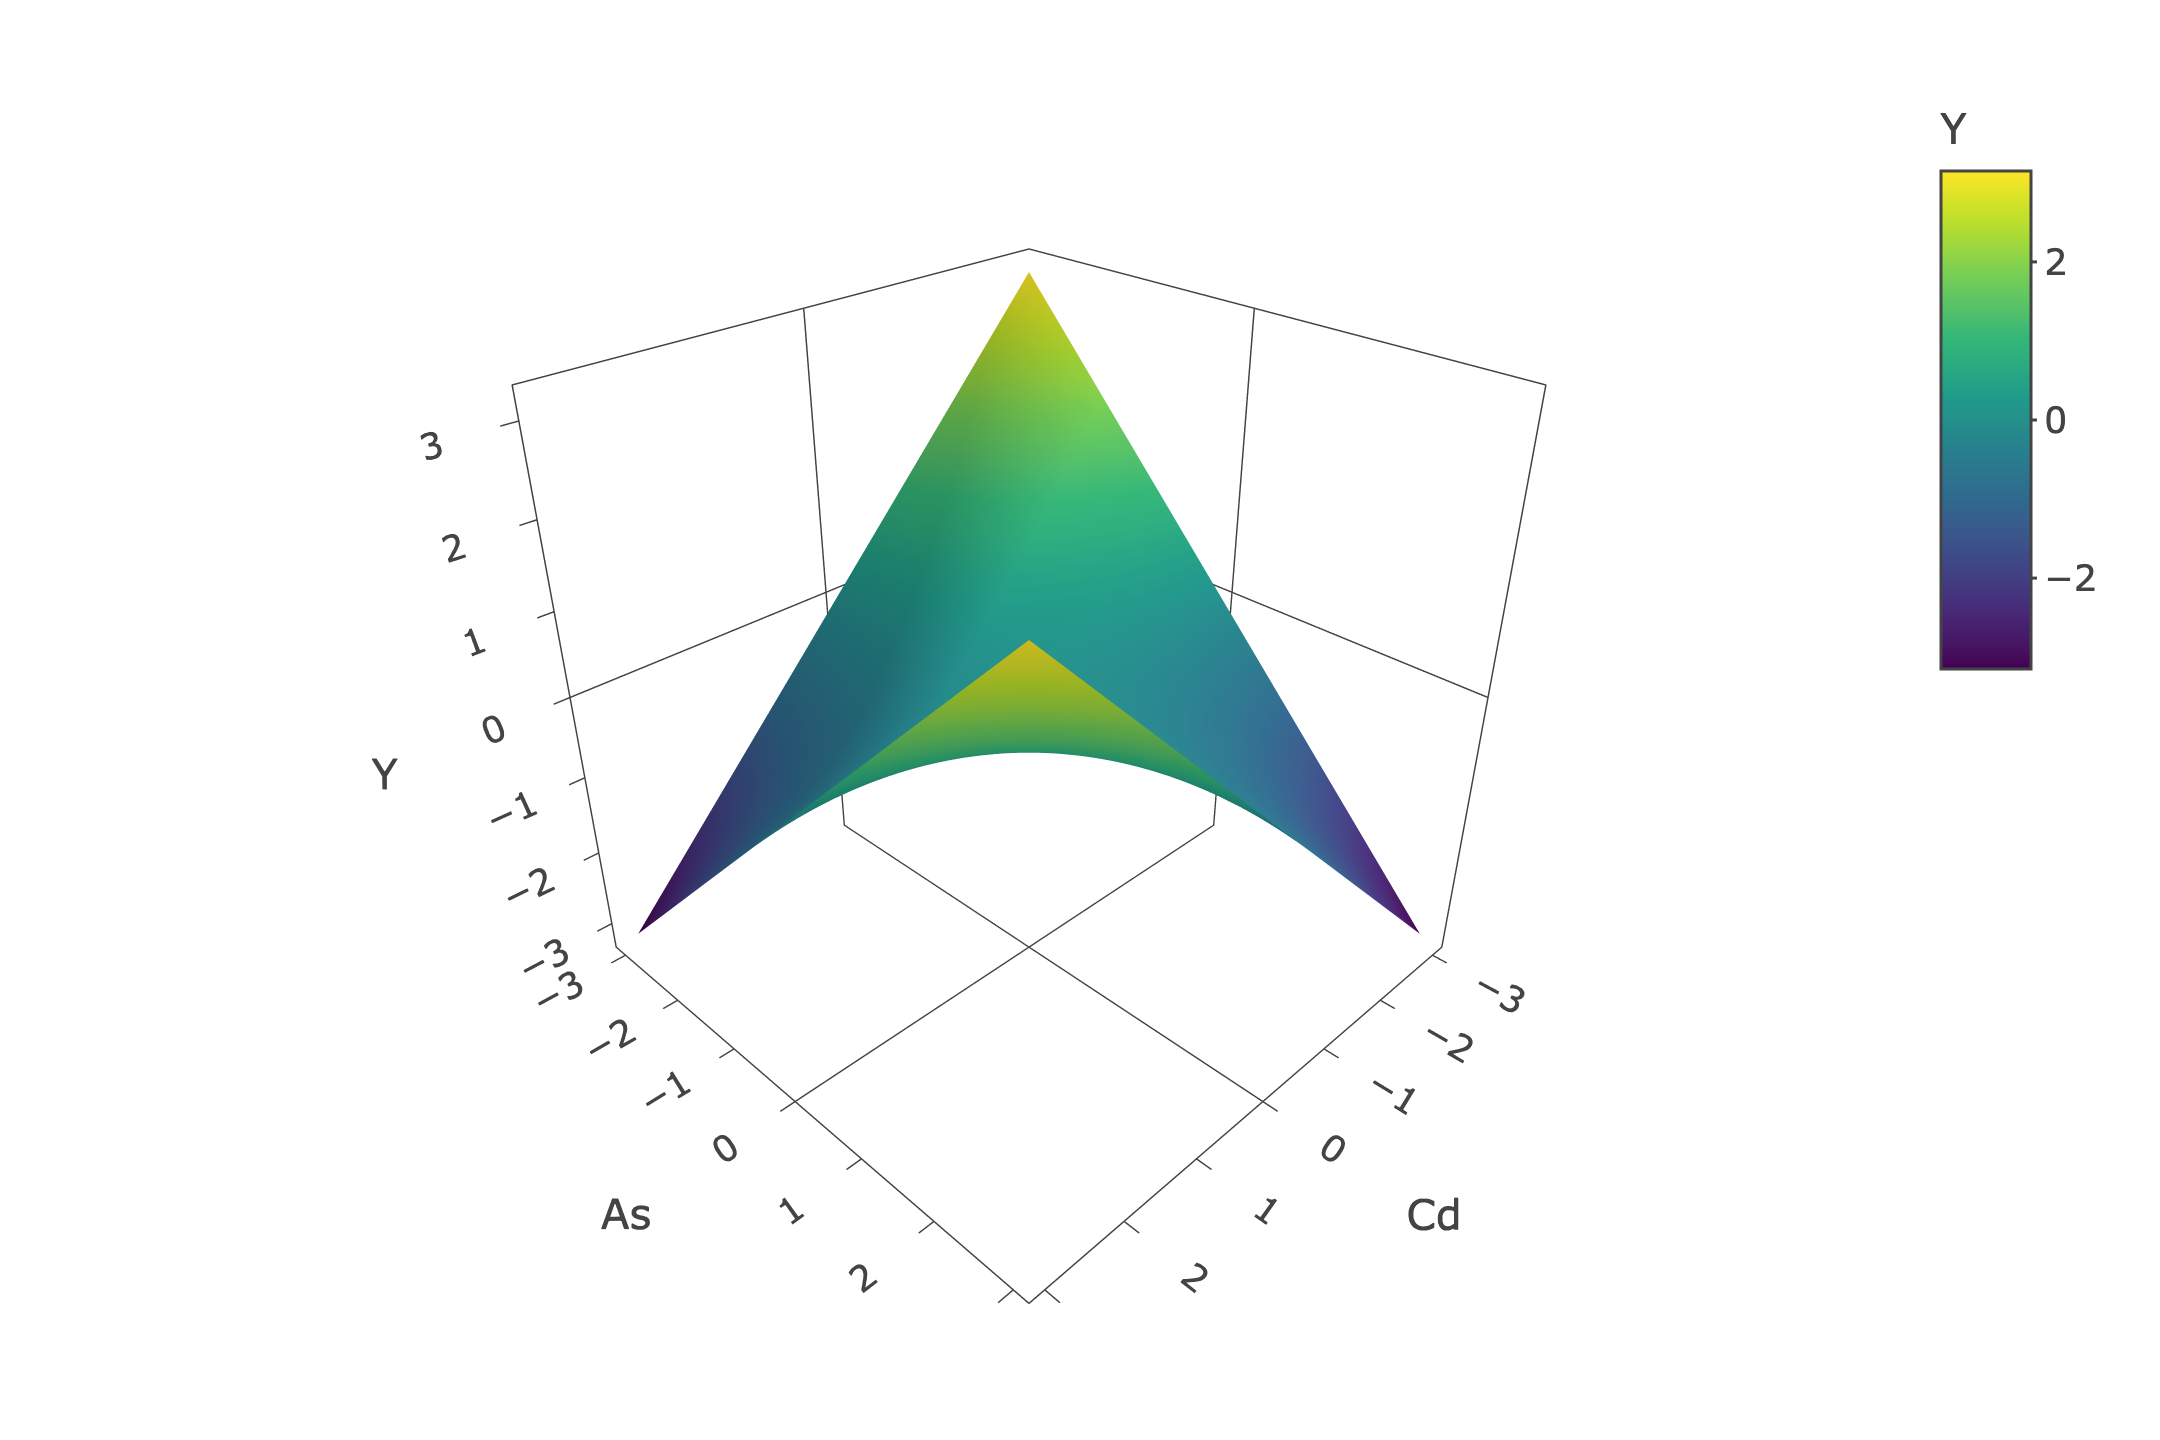
\includegraphics[width=0.5\linewidth]{figures/surfaces/bm1} 

}

\caption{Exposure-response surface for a multiplicative interaction between Cd and As at the lower effect size: $Y=$ 0.35Cd$*$As.}\label{fig:bm1}
\end{figure}
\begin{figure}

{\centering 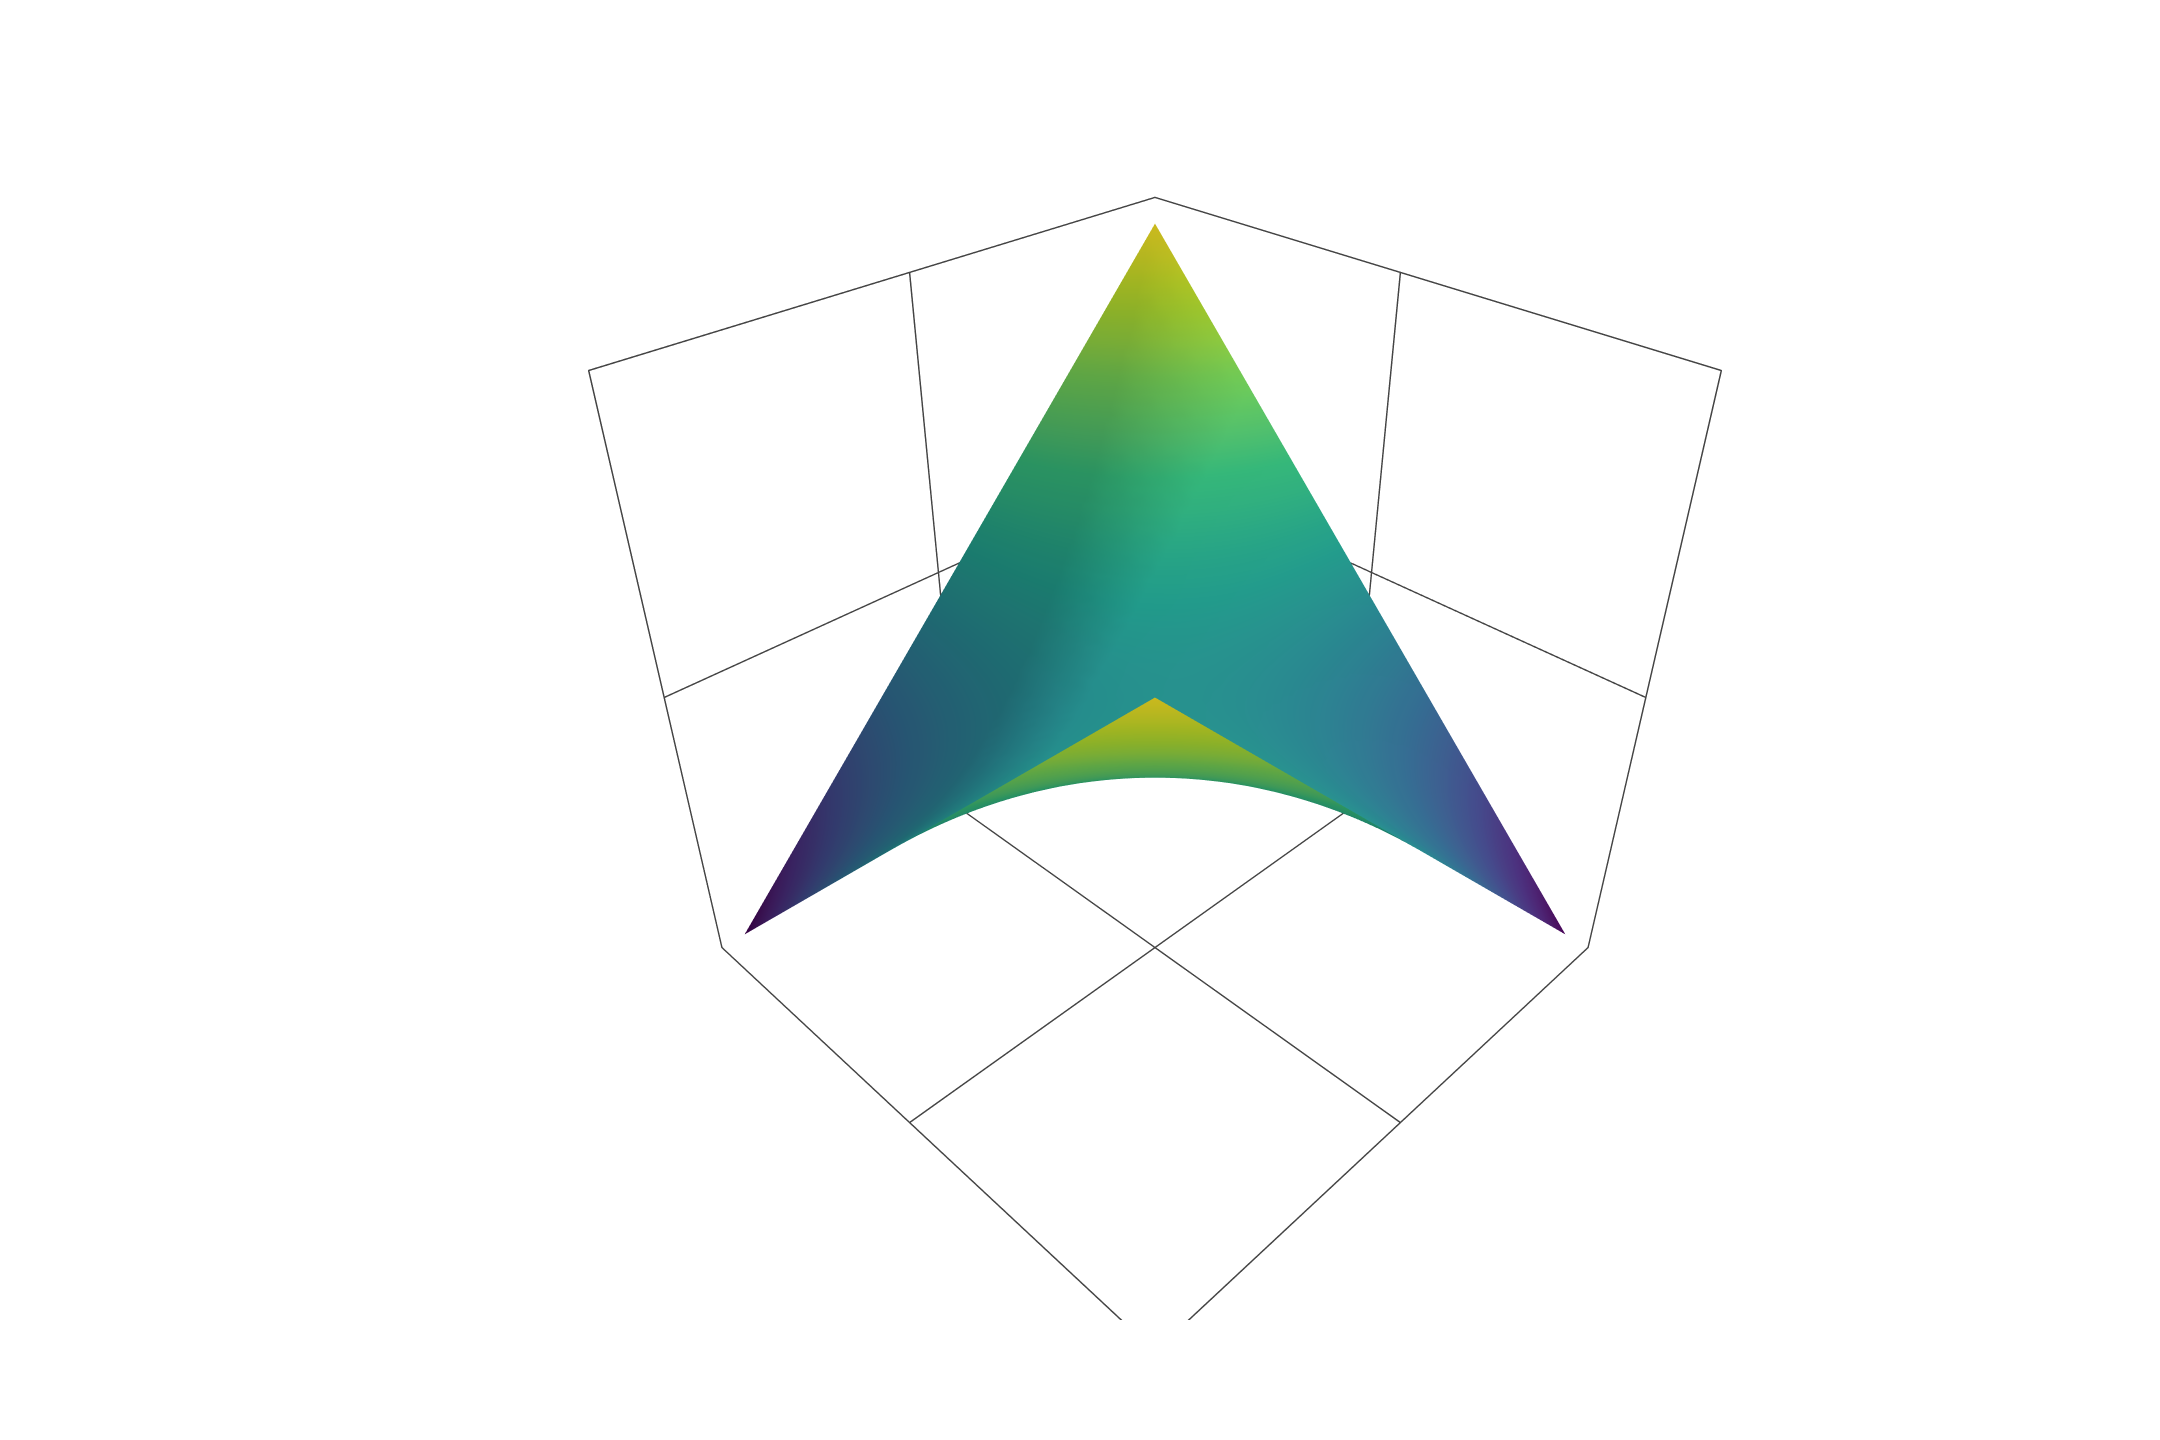
\includegraphics[width=0.5\linewidth]{figures/surfaces/bm2} 

}

\caption{Exposure-response surface for a multiplicative interaction between Cd and As at the higher effect size: $Y=$ 0.7Cd$*$As.}\label{fig:bm2}
\end{figure}
\begin{figure}

{\centering 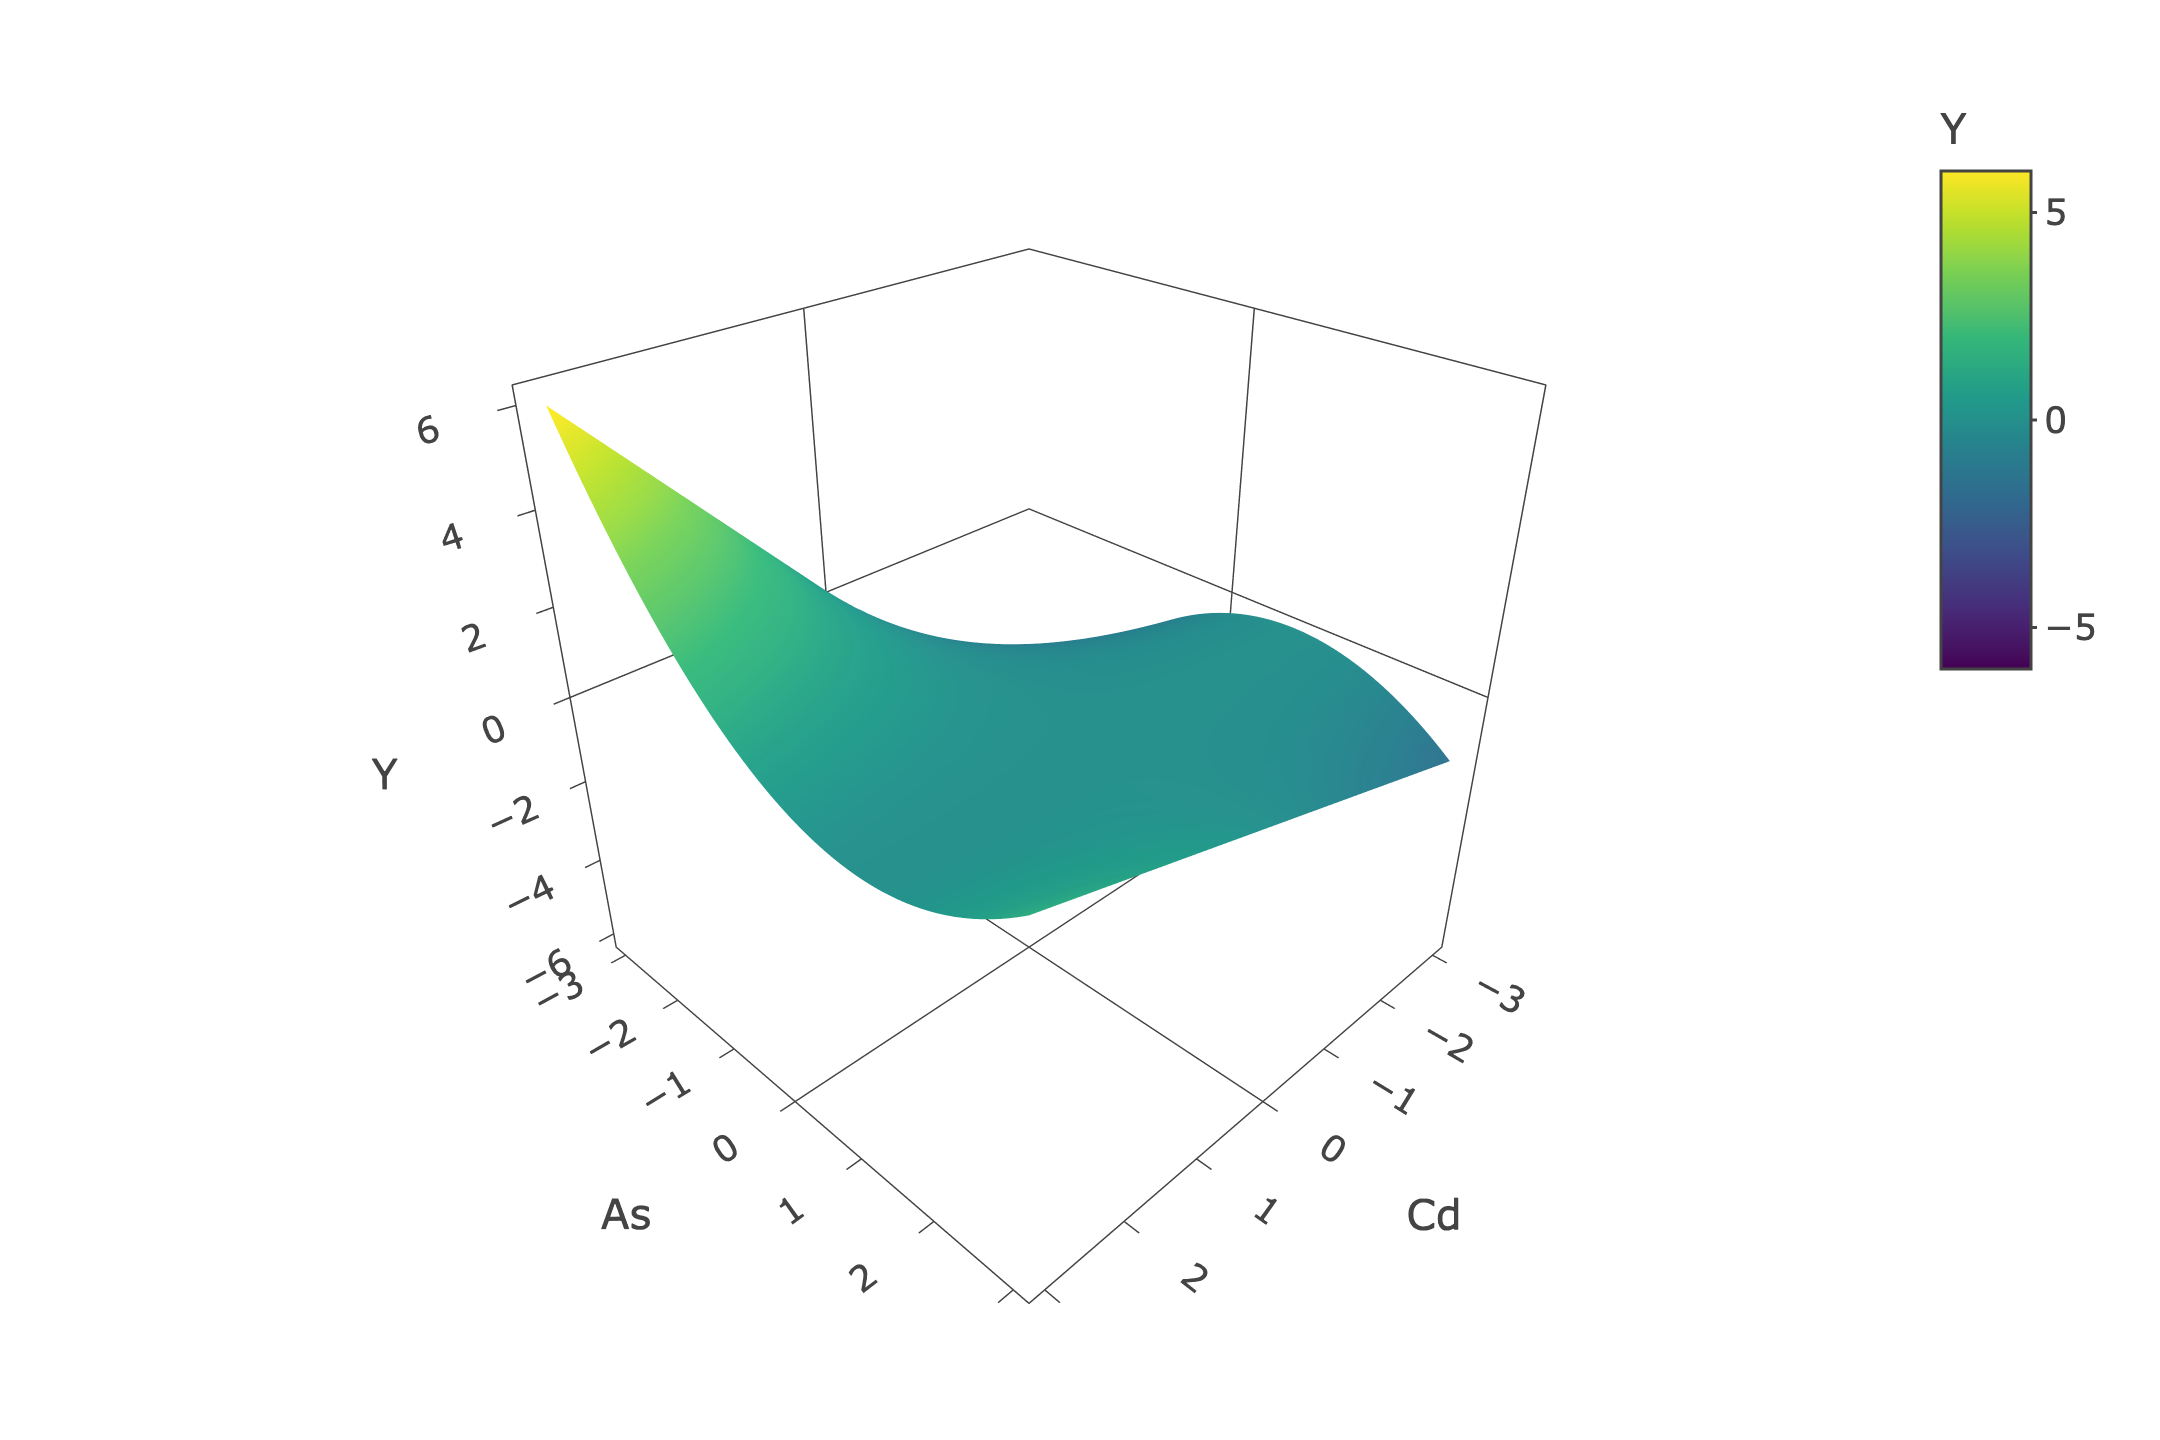
\includegraphics[width=0.5\linewidth]{figures/surfaces/bp1} 

}

\caption{Exposure-response surface for a polynomial interaction between Cd and As at the lower effect size: 0.125Cd$*($As$-1)^2$.}\label{fig:bp1}
\end{figure}
\begin{figure}

{\centering 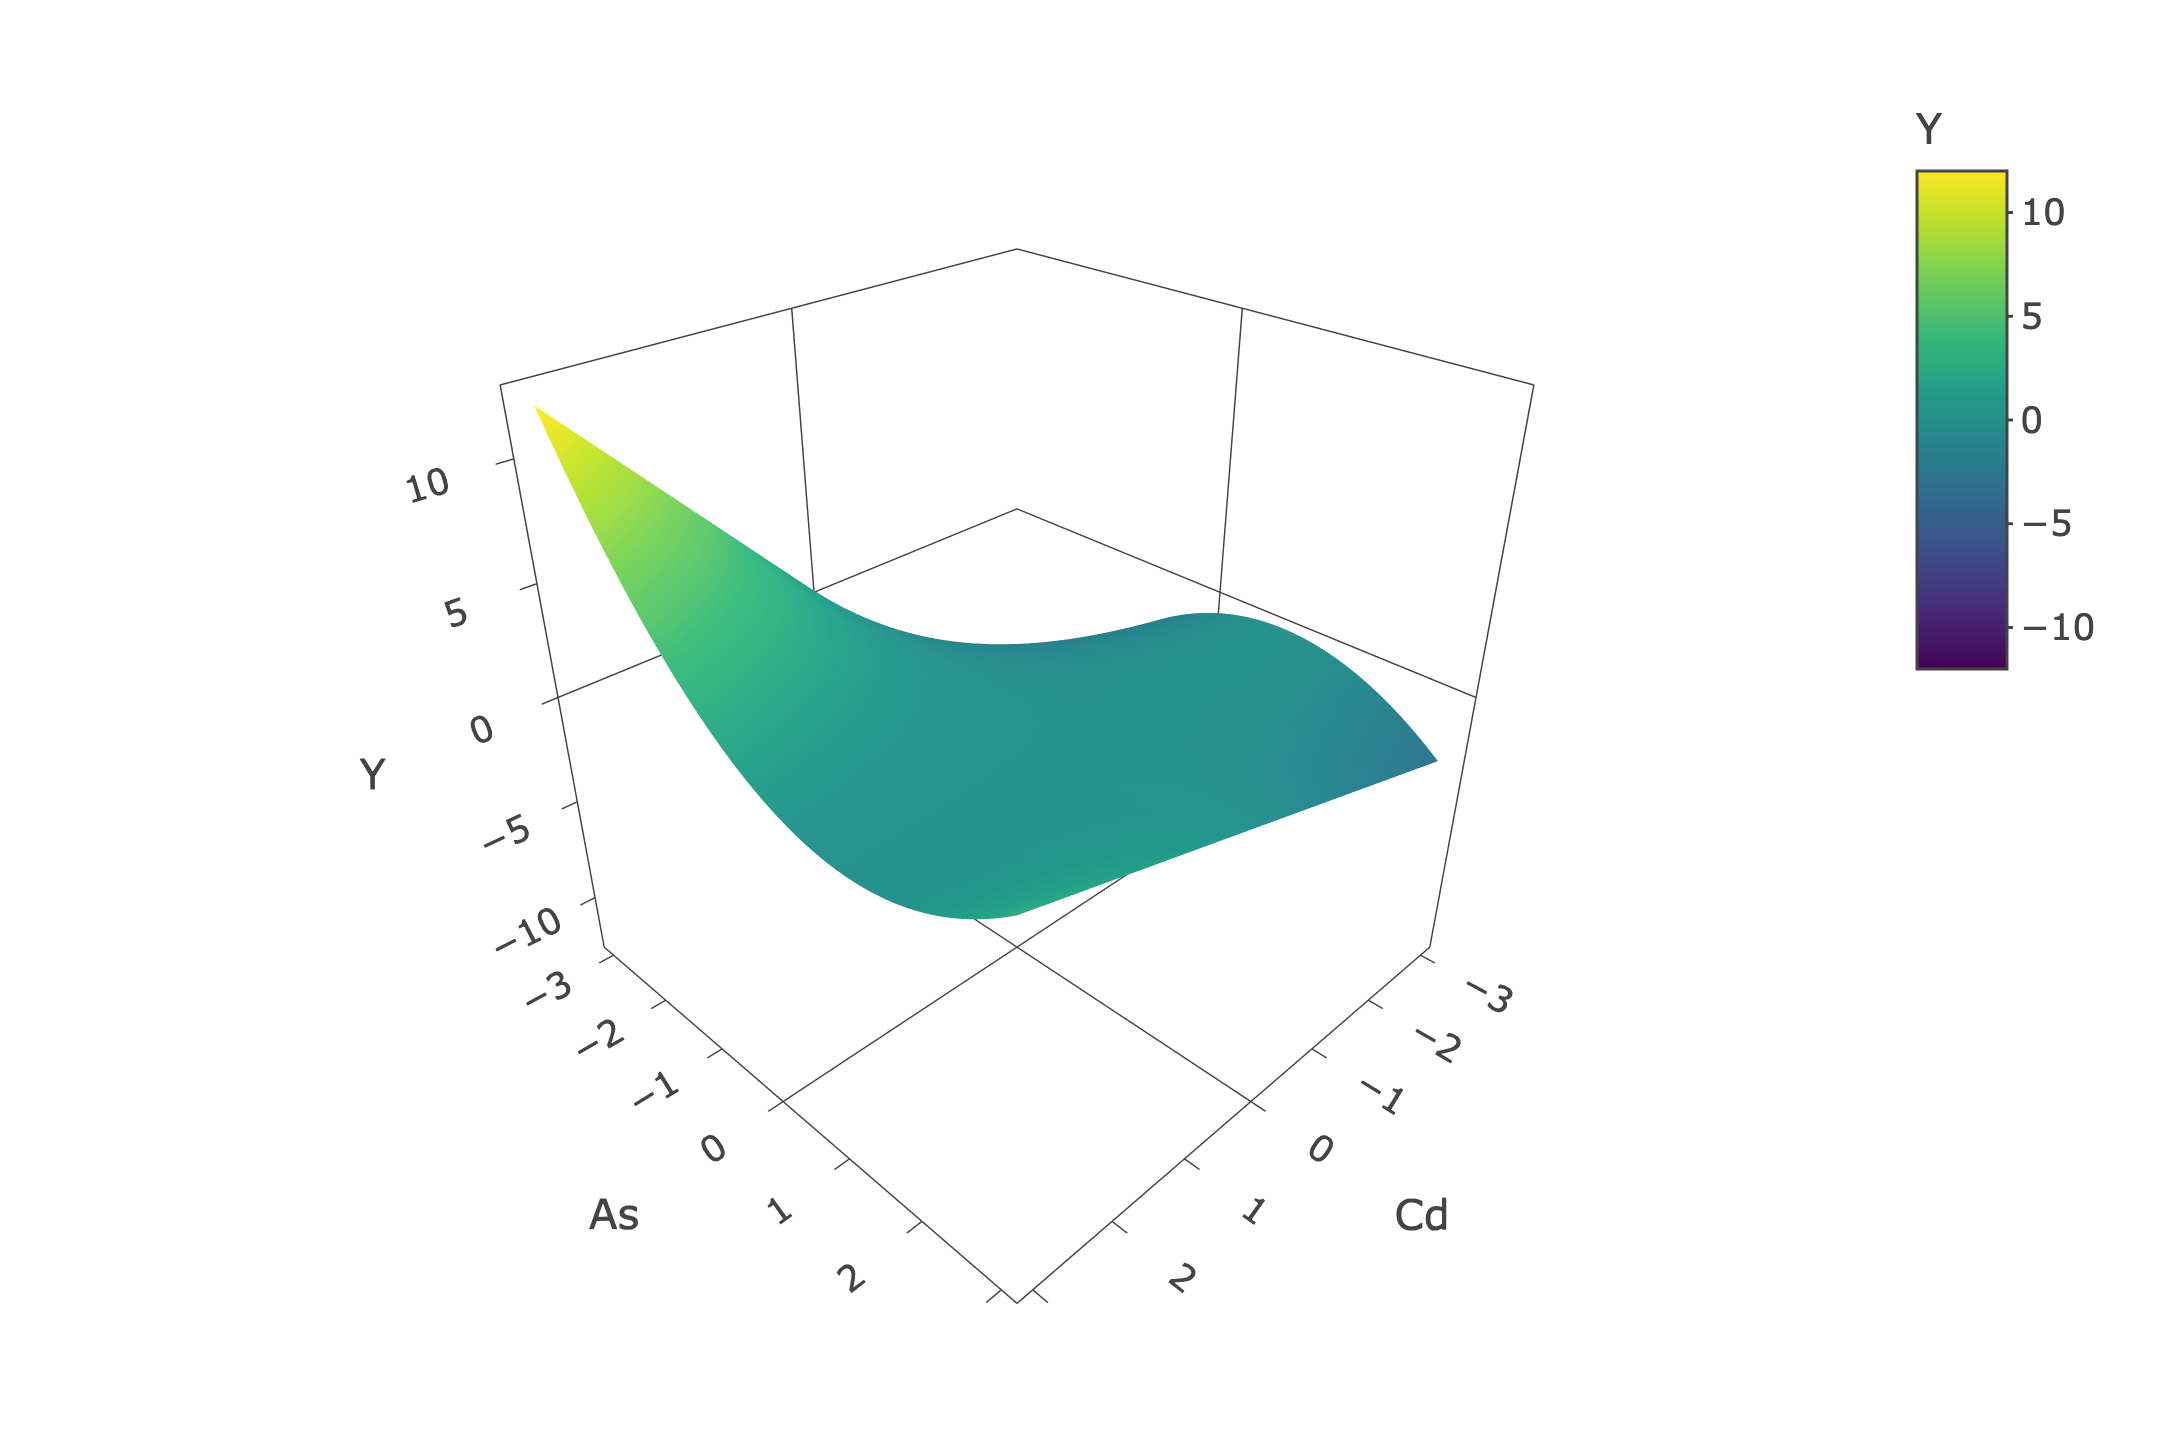
\includegraphics[width=0.5\linewidth]{figures/surfaces/bp2} 

}

\caption{Exposure-response surface for a polynomial interaction between Cd and As at the higher effect size: 0.25Cd$*($As$-1)^2$.}\label{fig:bp2}
\end{figure}
\begin{figure}

{\centering 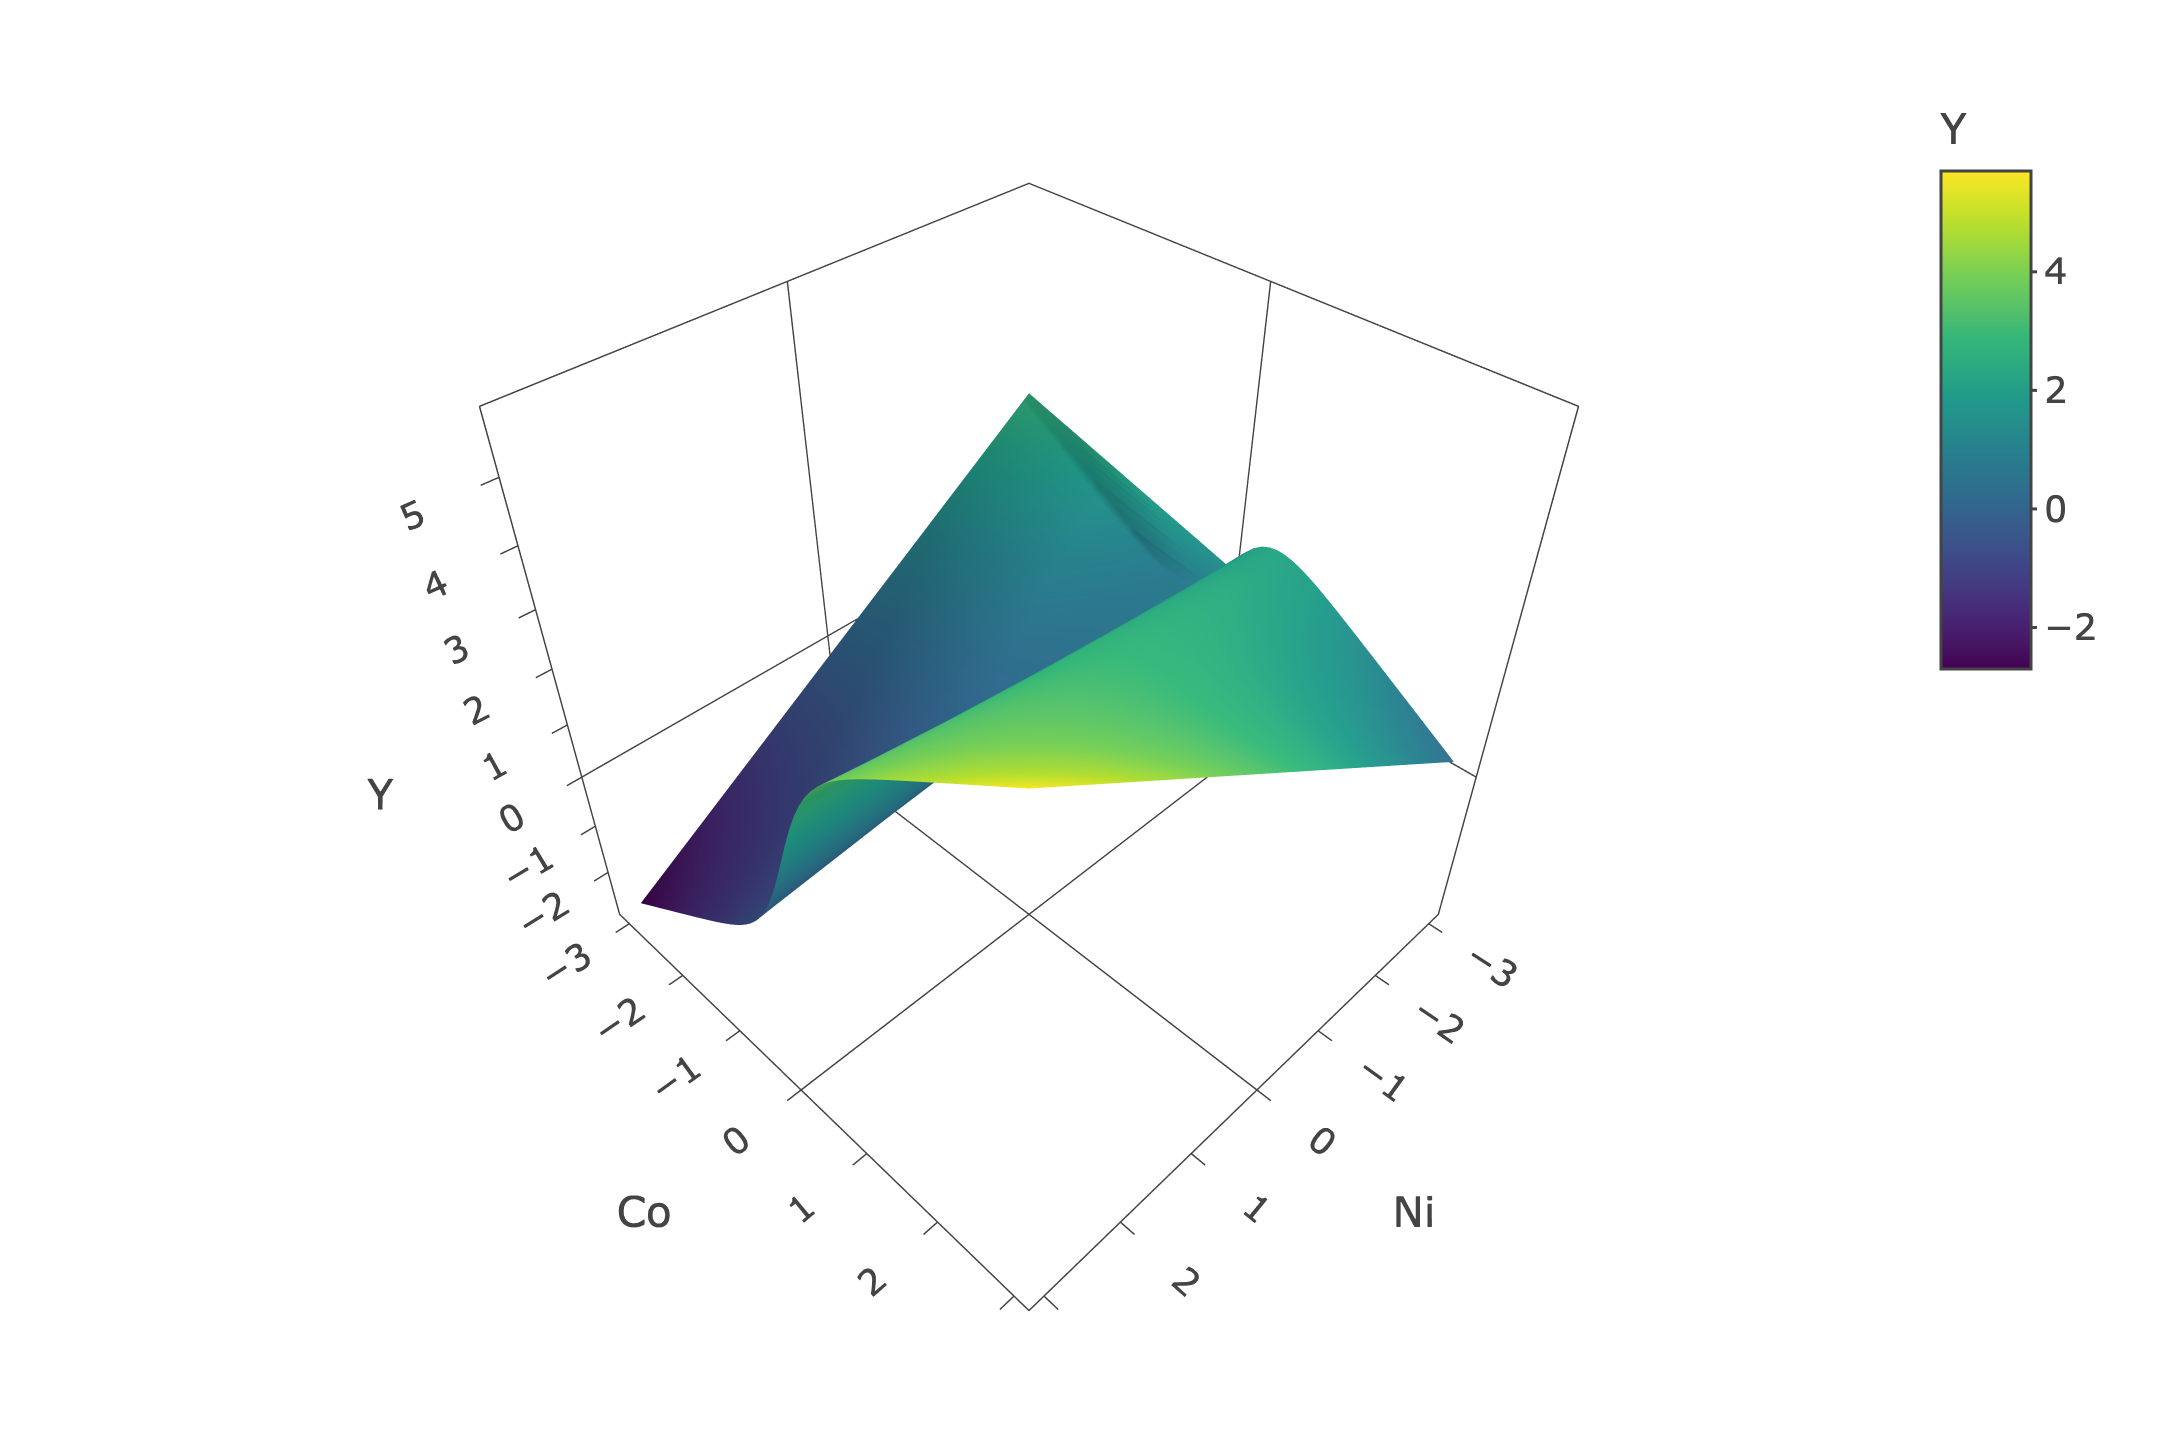
\includegraphics[width=0.5\linewidth]{figures/surfaces/cm1} 

}

\caption{Exposure-response surface for a multiplicative interaction between Ni and Co at the lower effect size: $Y=$ $\frac{3}{1+\textrm{exp}(-4\textrm{Ni})}$ + 0.3Ni$*$Co.}\label{fig:cm1}
\end{figure}
\begin{figure}

{\centering 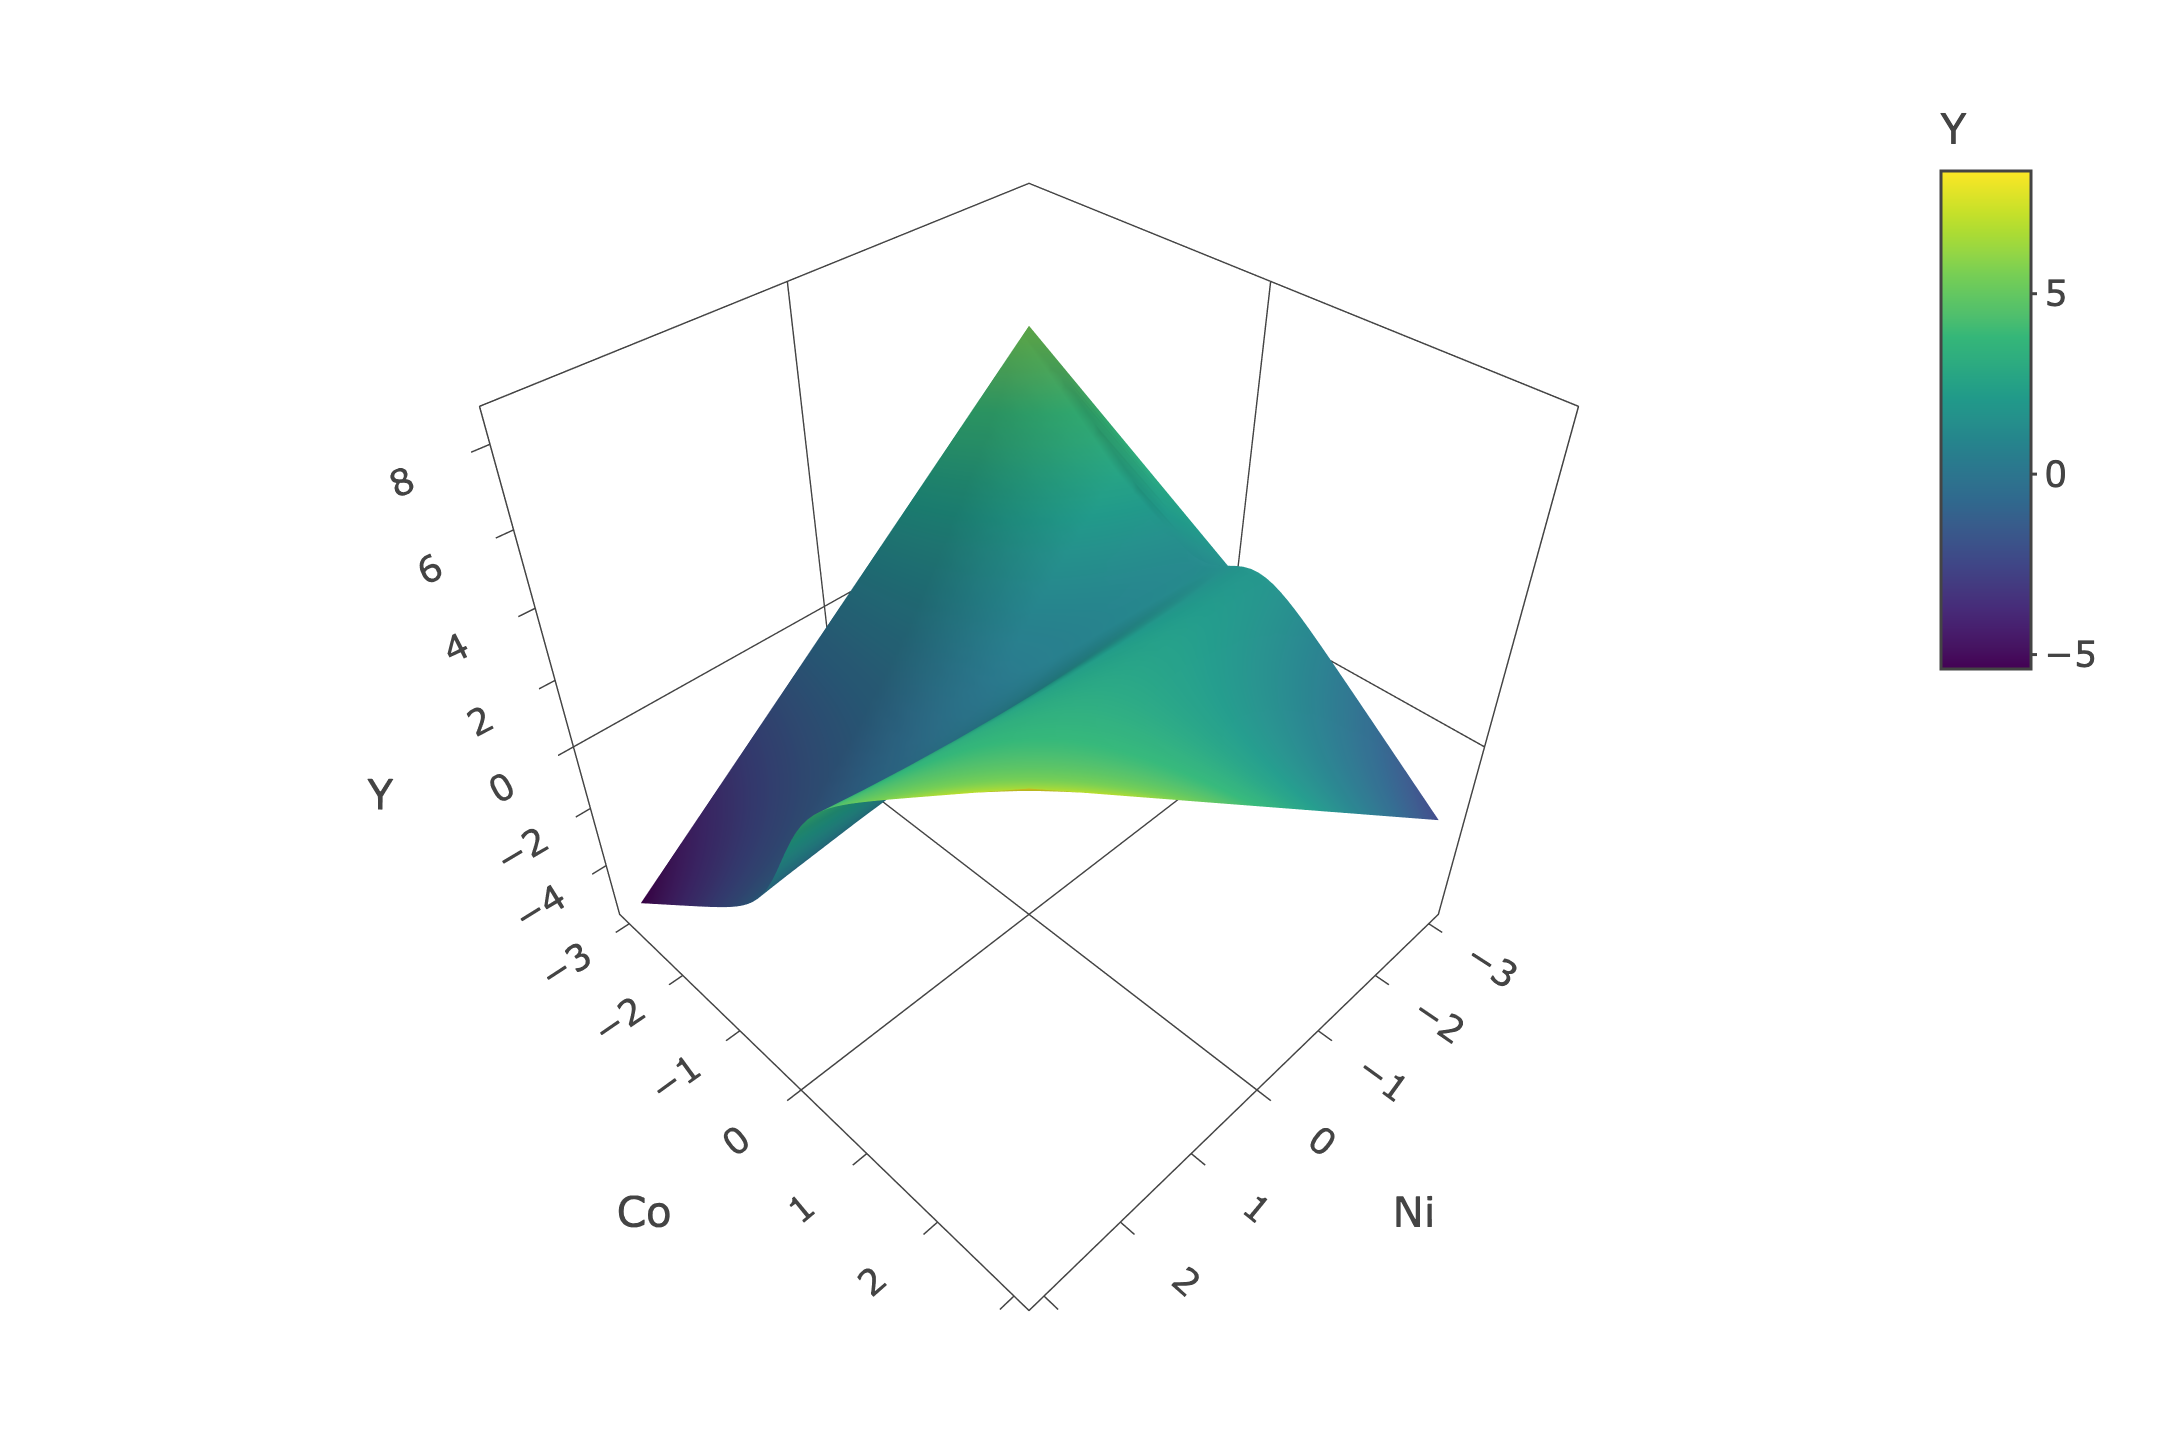
\includegraphics[width=0.5\linewidth]{figures/surfaces/cm2} 

}

\caption{Exposure-response surface for a multiplicative interaction between Ni and Co at the higher effect size: $Y=$ $\frac{3}{1+\textrm{exp}(-4\textrm{Ni})}$ + 0.6Ni$*$Co.}\label{fig:cm2}
\end{figure}
\begin{figure}

{\centering 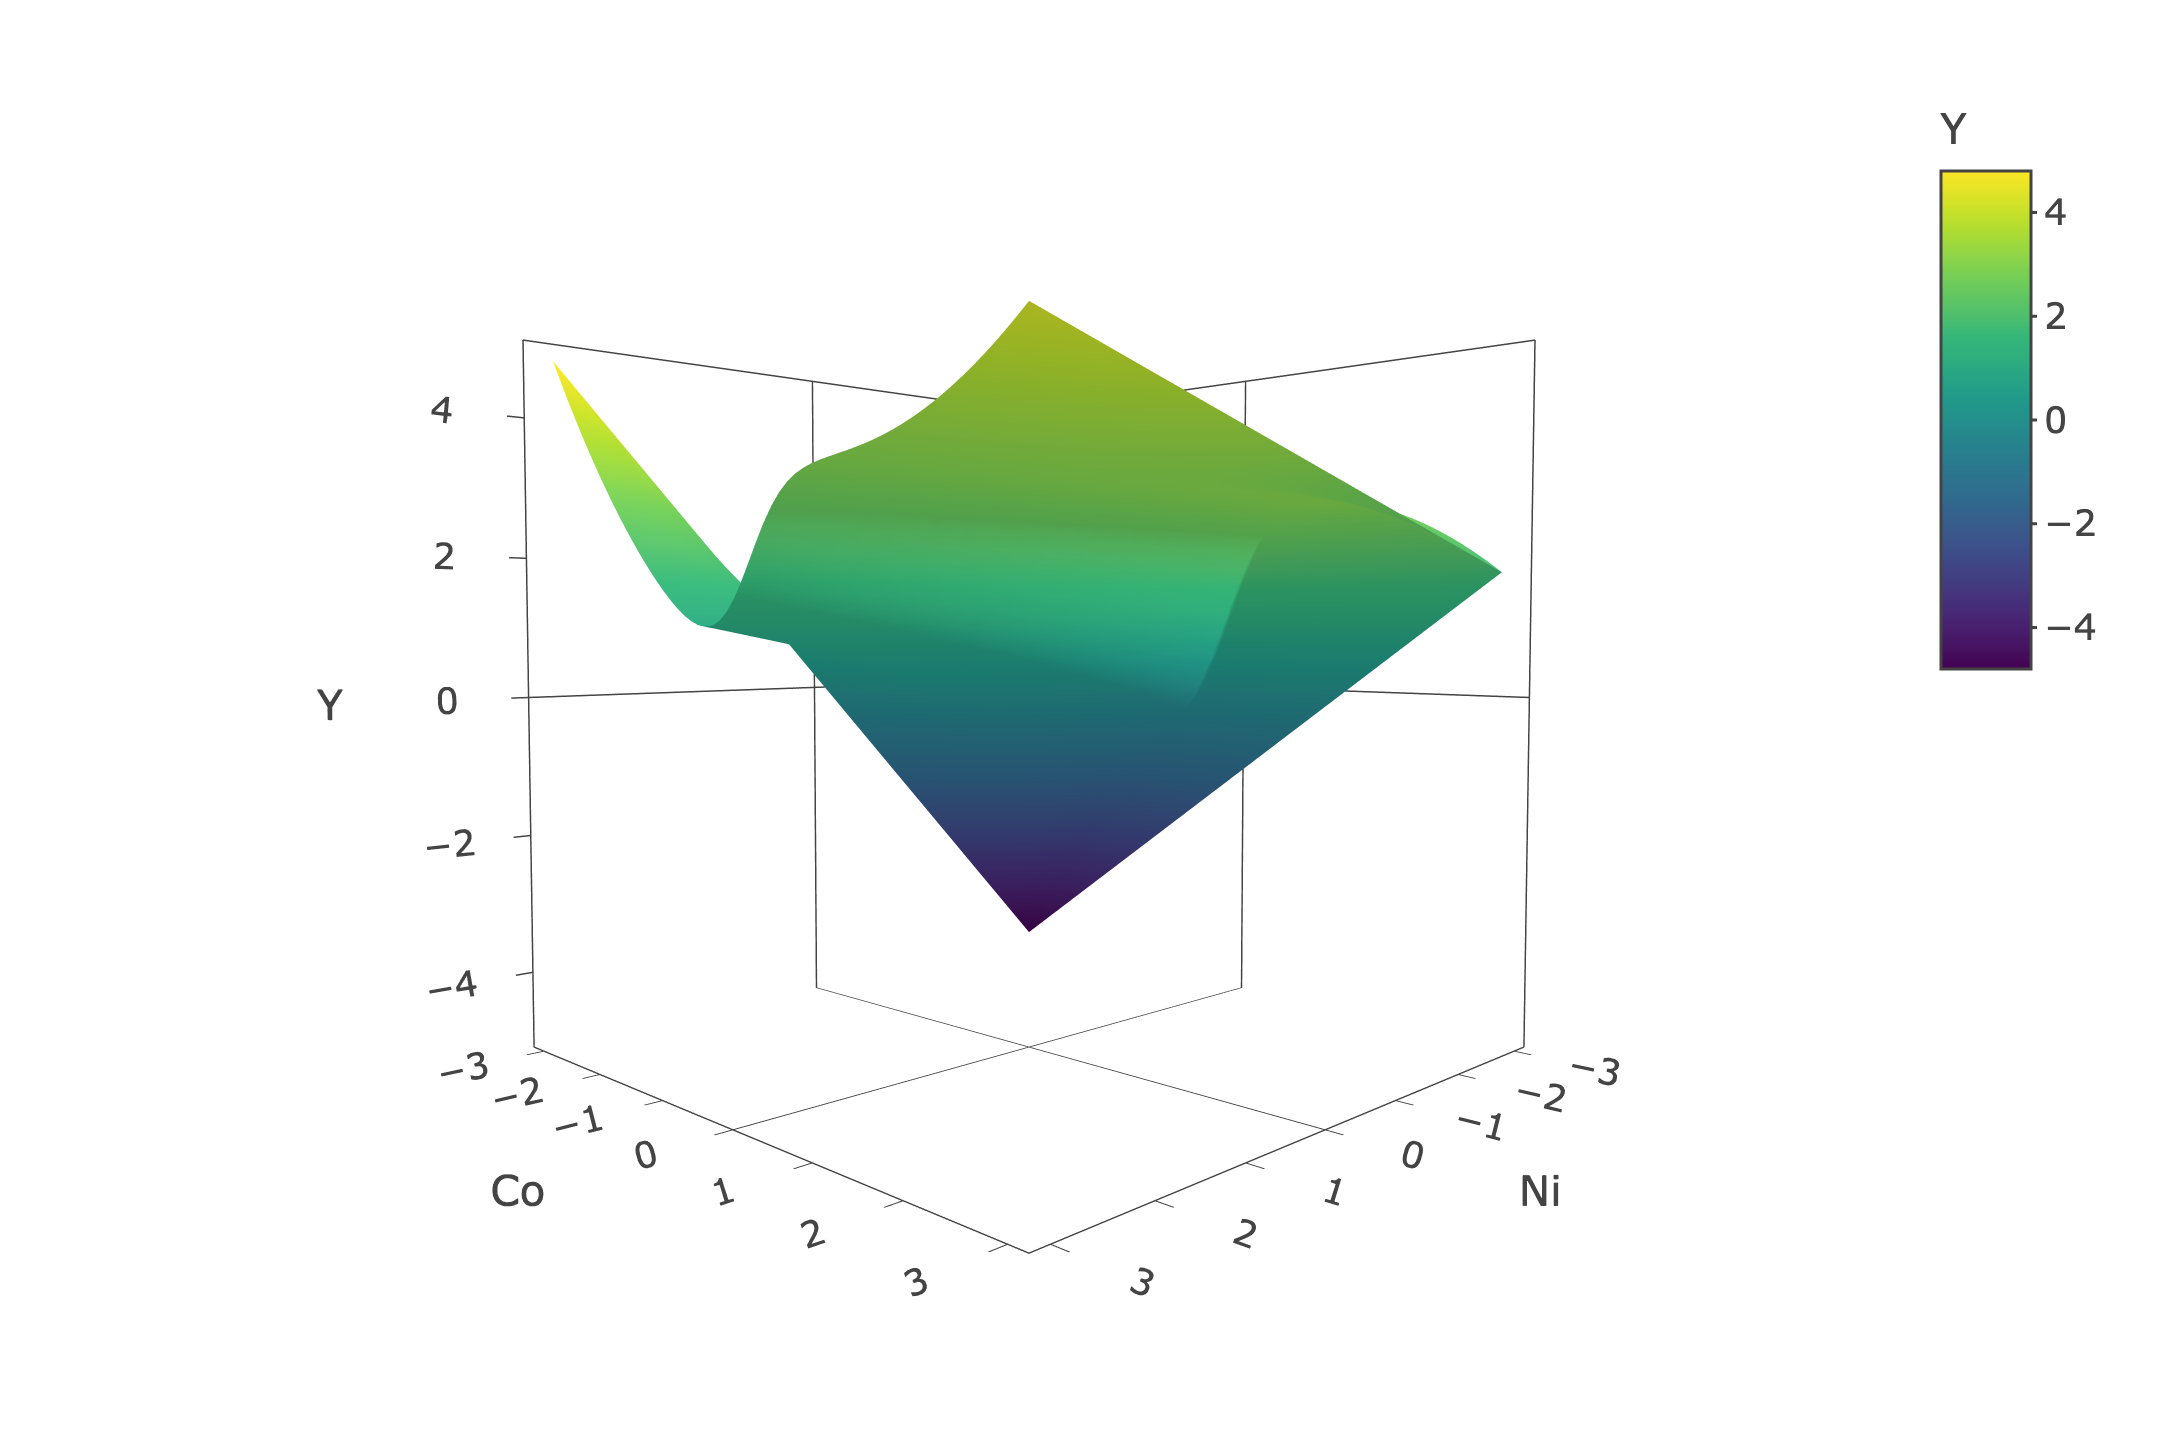
\includegraphics[width=0.5\linewidth]{figures/surfaces/cp1} 

}

\caption{Exposure-response surface for a polynomial interaction between Ni and Co at the lower effect size: $Y=$ $\frac{3}{1+\textrm{exp}(-4\textrm{Ni})}$ + 0.09Ni$*($Co$-1)^2$.}\label{fig:cp1}
\end{figure}
\begin{figure}

{\centering 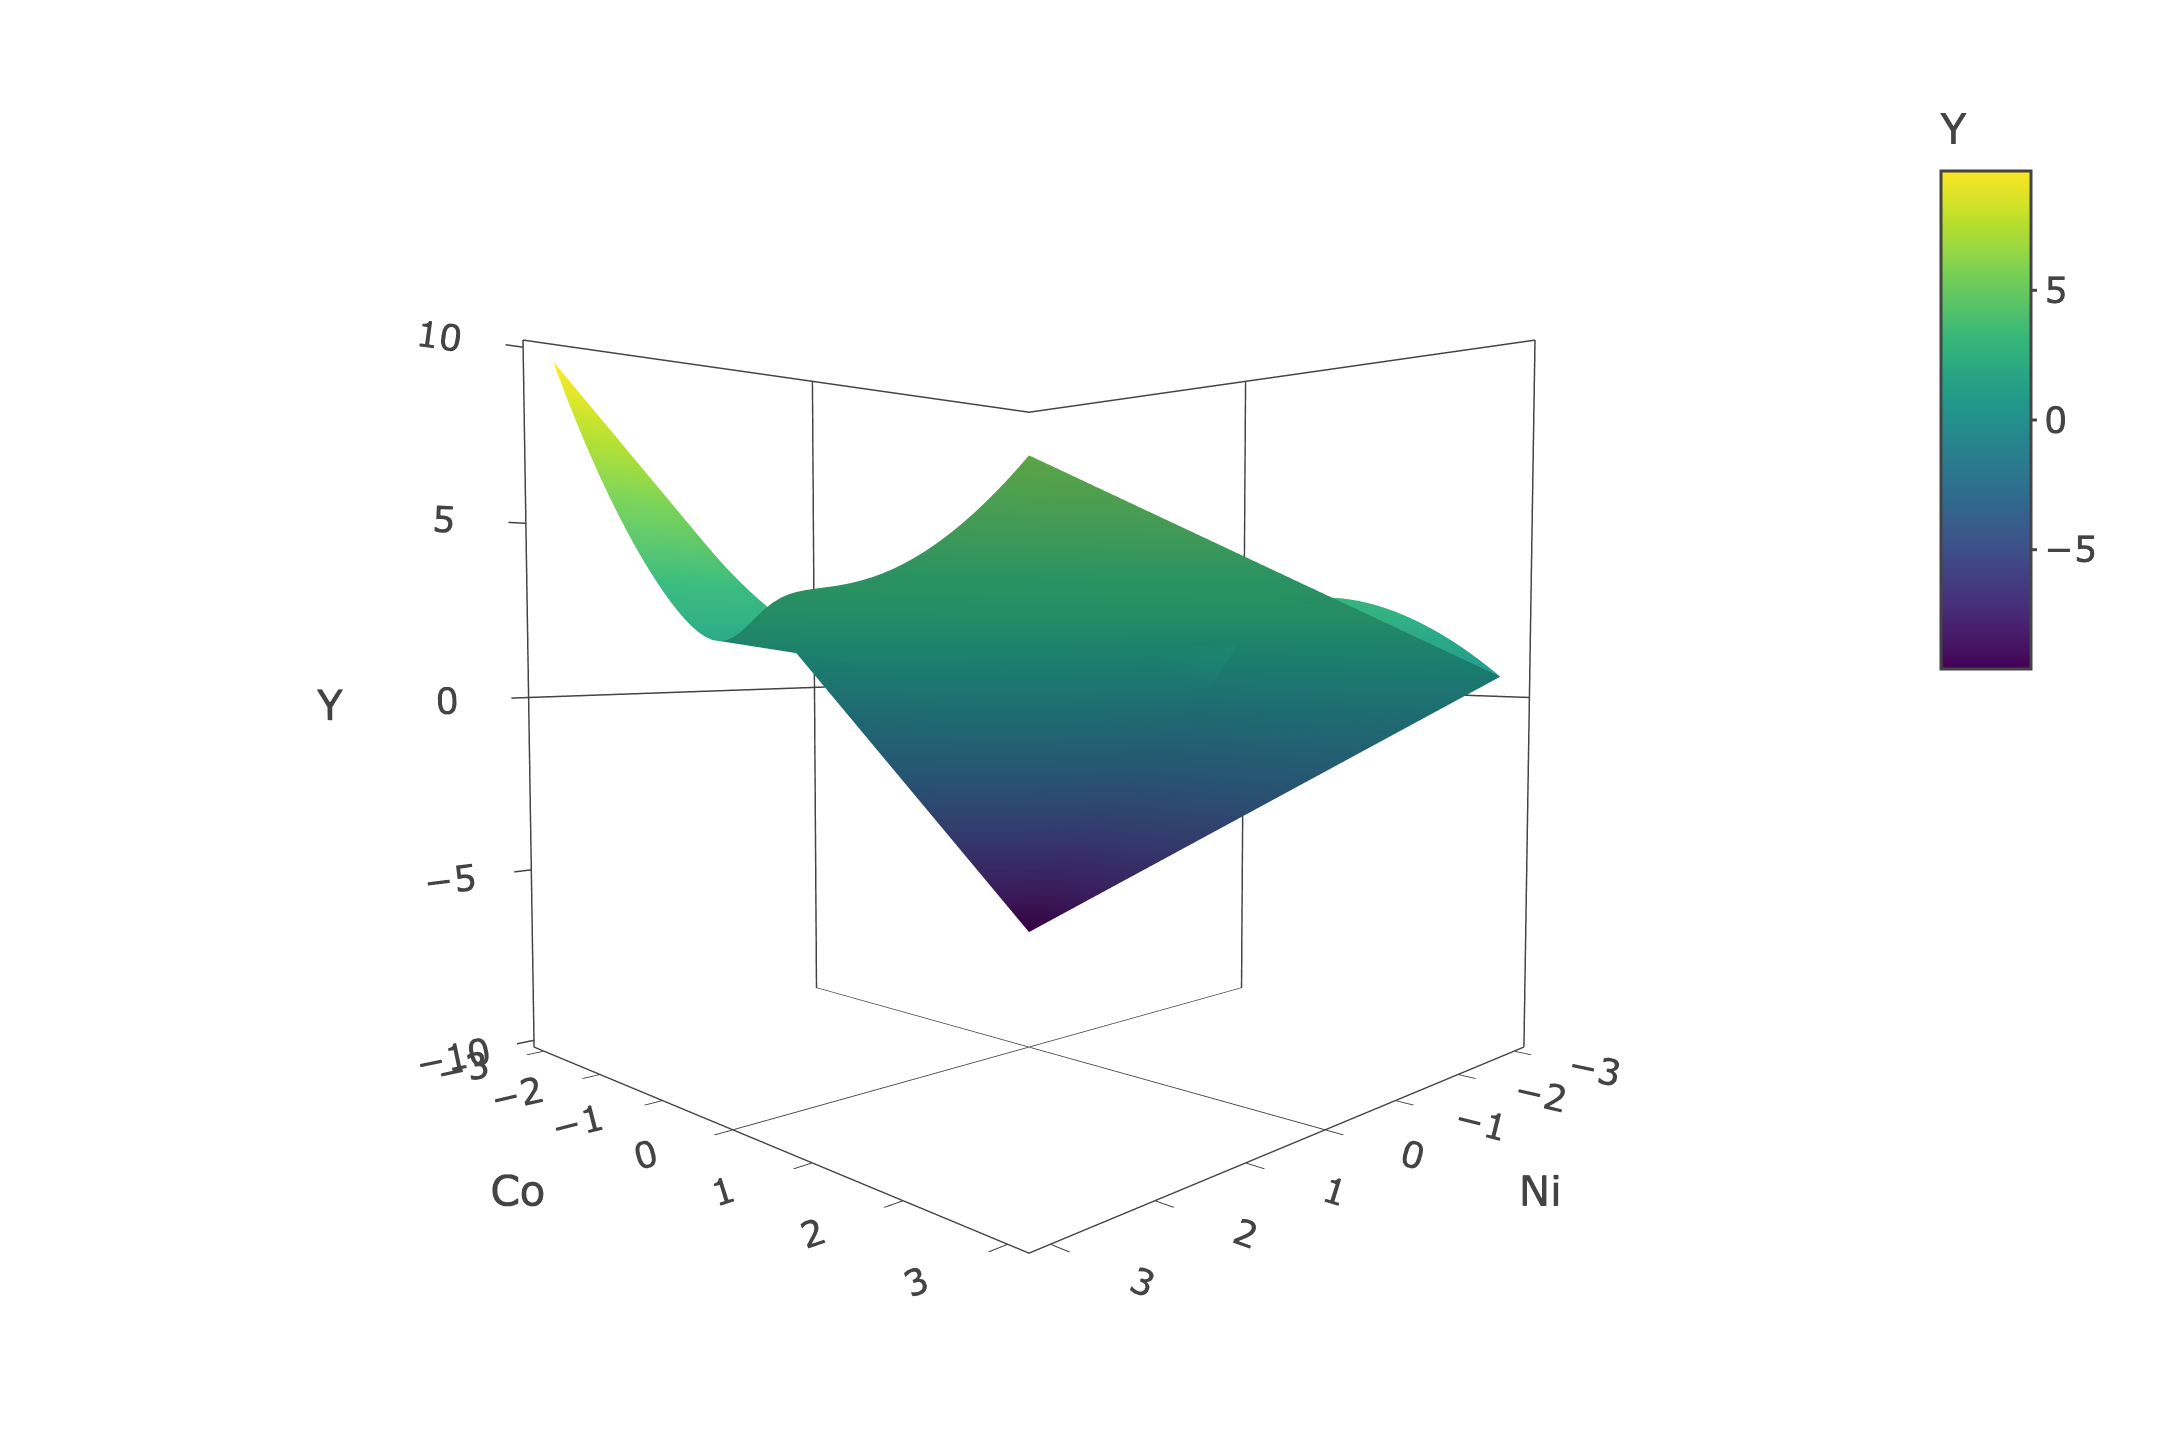
\includegraphics[width=0.5\linewidth]{figures/surfaces/cp2} 

}

\caption{Exposure-response surface for a polynomial interaction between Ni and Co at the lower effect size: $Y=$ $\frac{3}{1+\textrm{exp}(-4\textrm{Ni})}$ + 0.18Ni$*($Co$-1)^2$.}\label{fig:cp2}
\end{figure}
Figure \ref{fig:cordistsm} shows the detailed distribution of correlations in smaller size simulated datasets.
\begin{figure}

{\centering 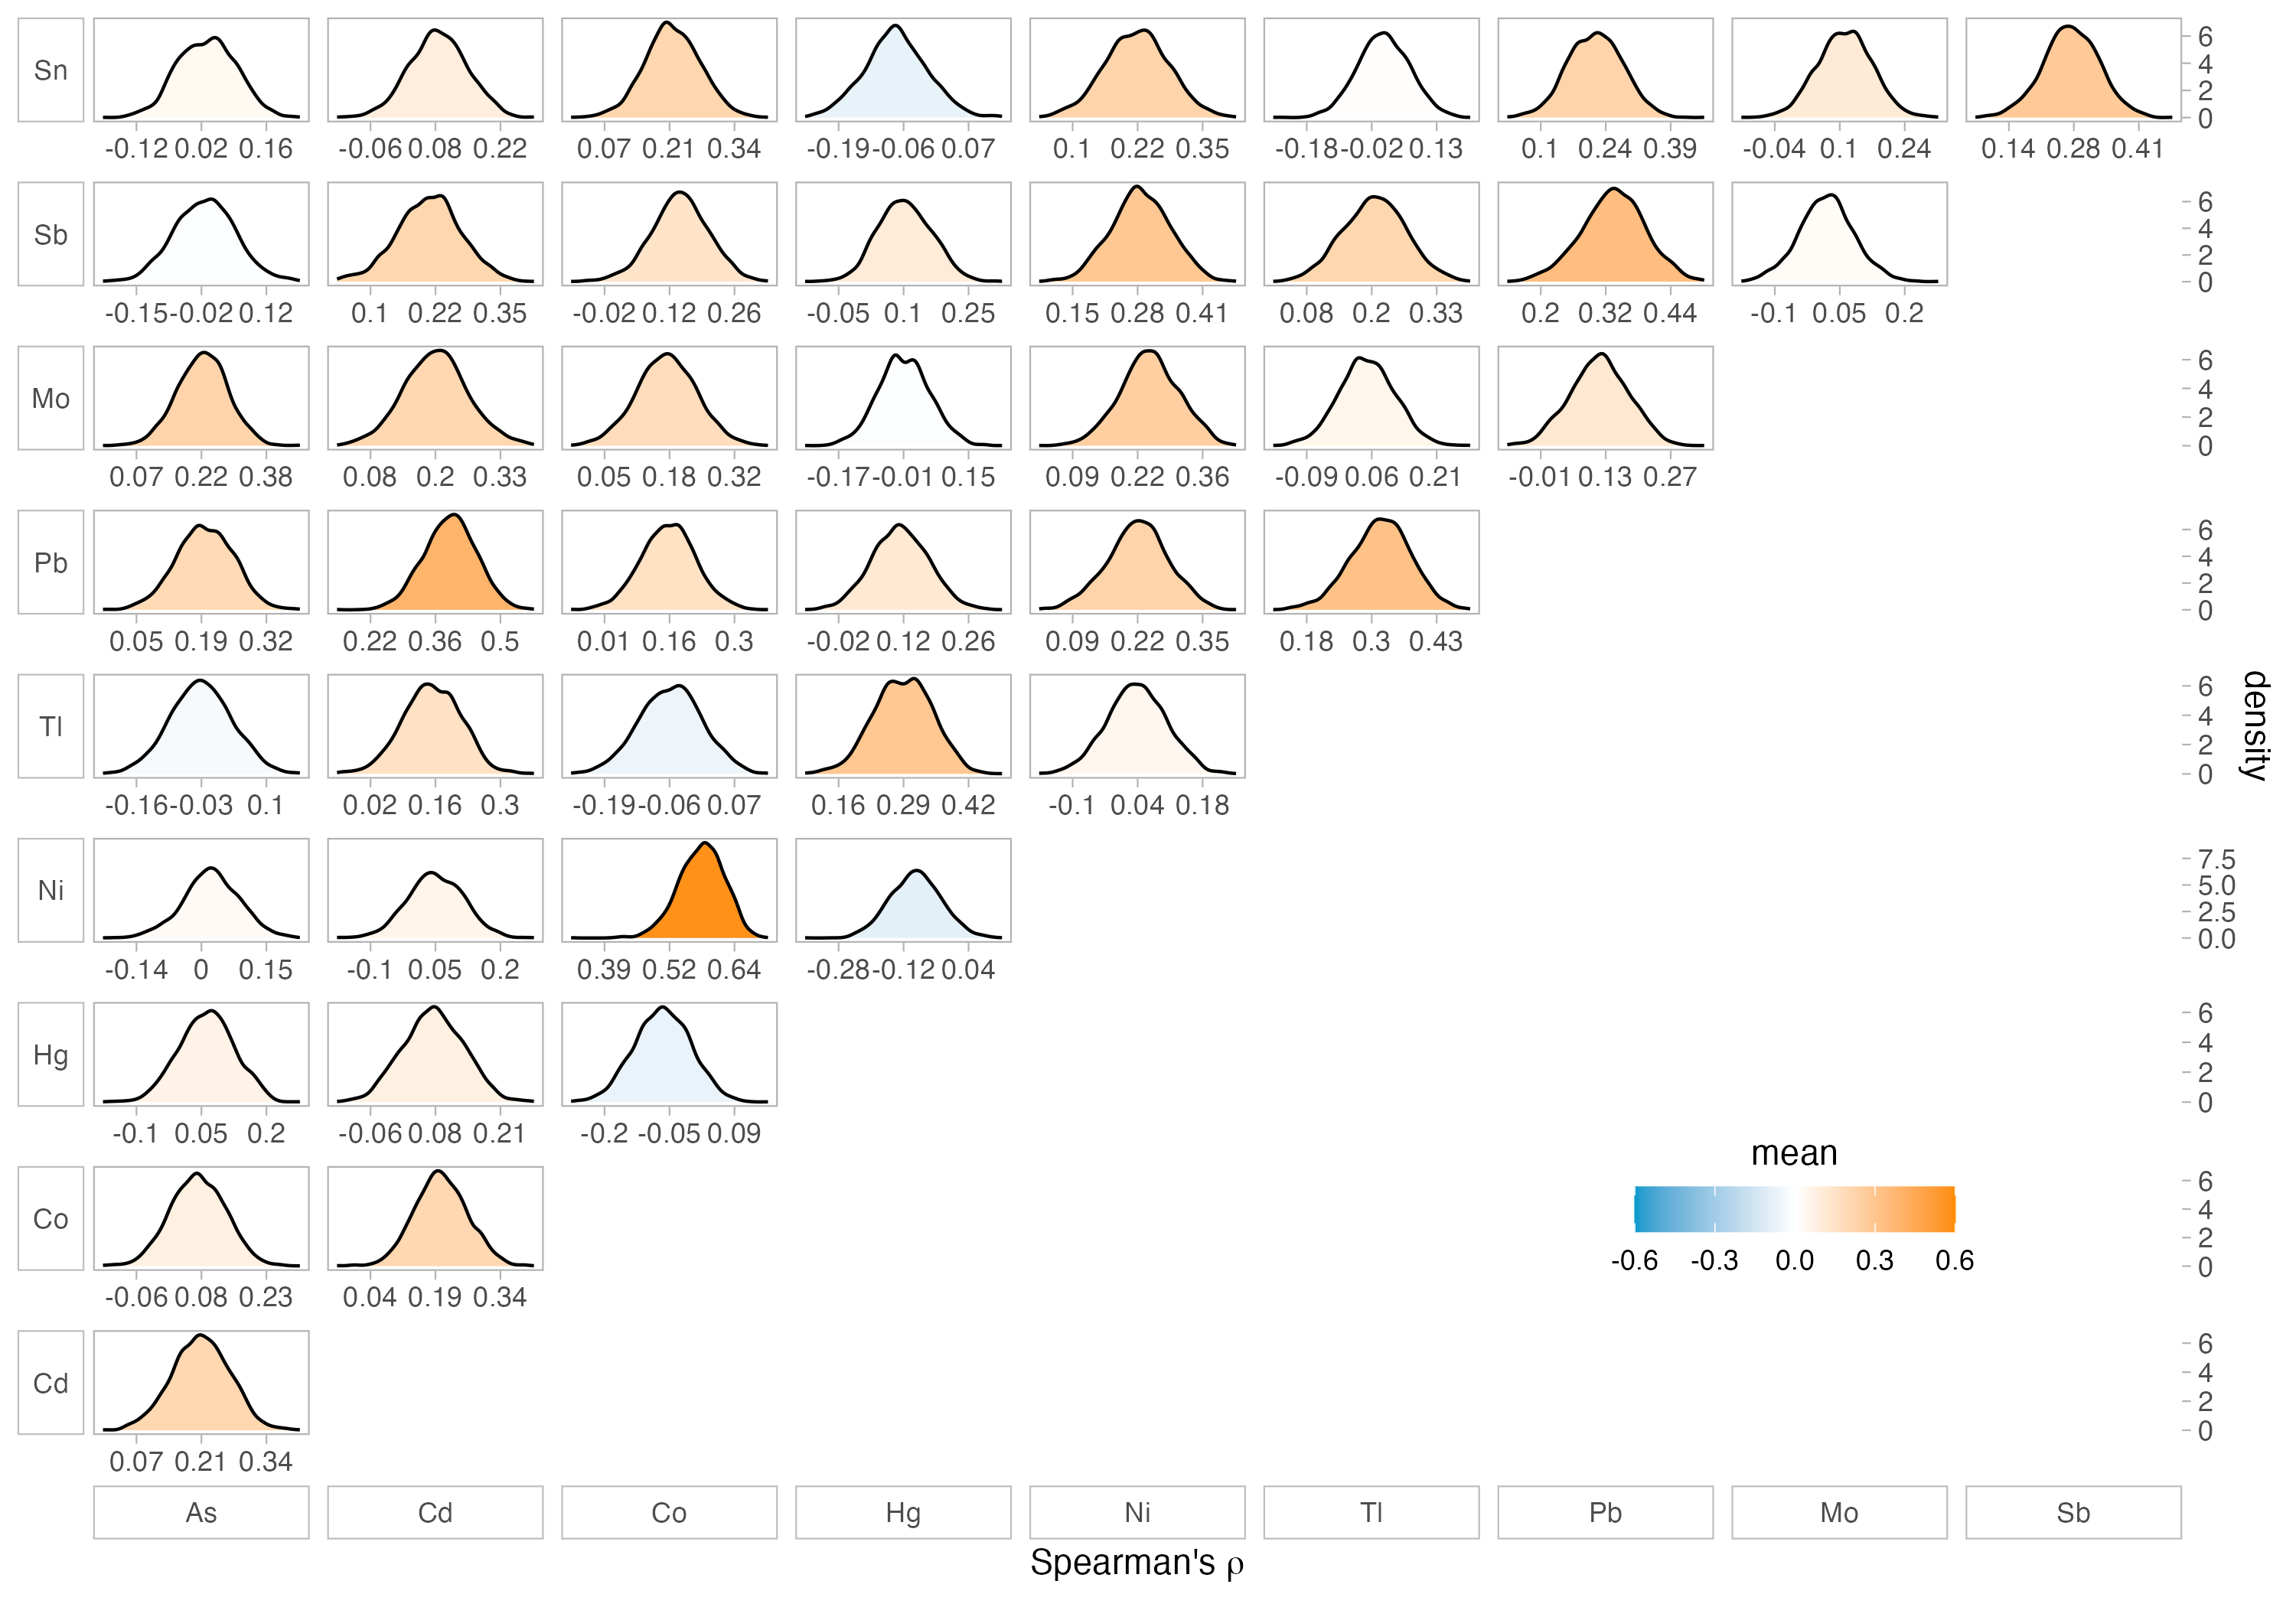
\includegraphics[width=1\linewidth]{figures/ch4_corr_sim} 

}

\caption{Distributions of Spearman's correlation from 2100 smaller size (n=252) simulated datasets.}\label{fig:cordistsm}
\end{figure}
Figures \ref{fig:univexplg}, \ref{fig:univcovlg}, and \ref{fig:corsimslg} compare the marginal distributions of predictors and dependence structure between exposures of the observed dataset and simulated datasets of larger size (n=1000).
\begin{figure}

{\centering 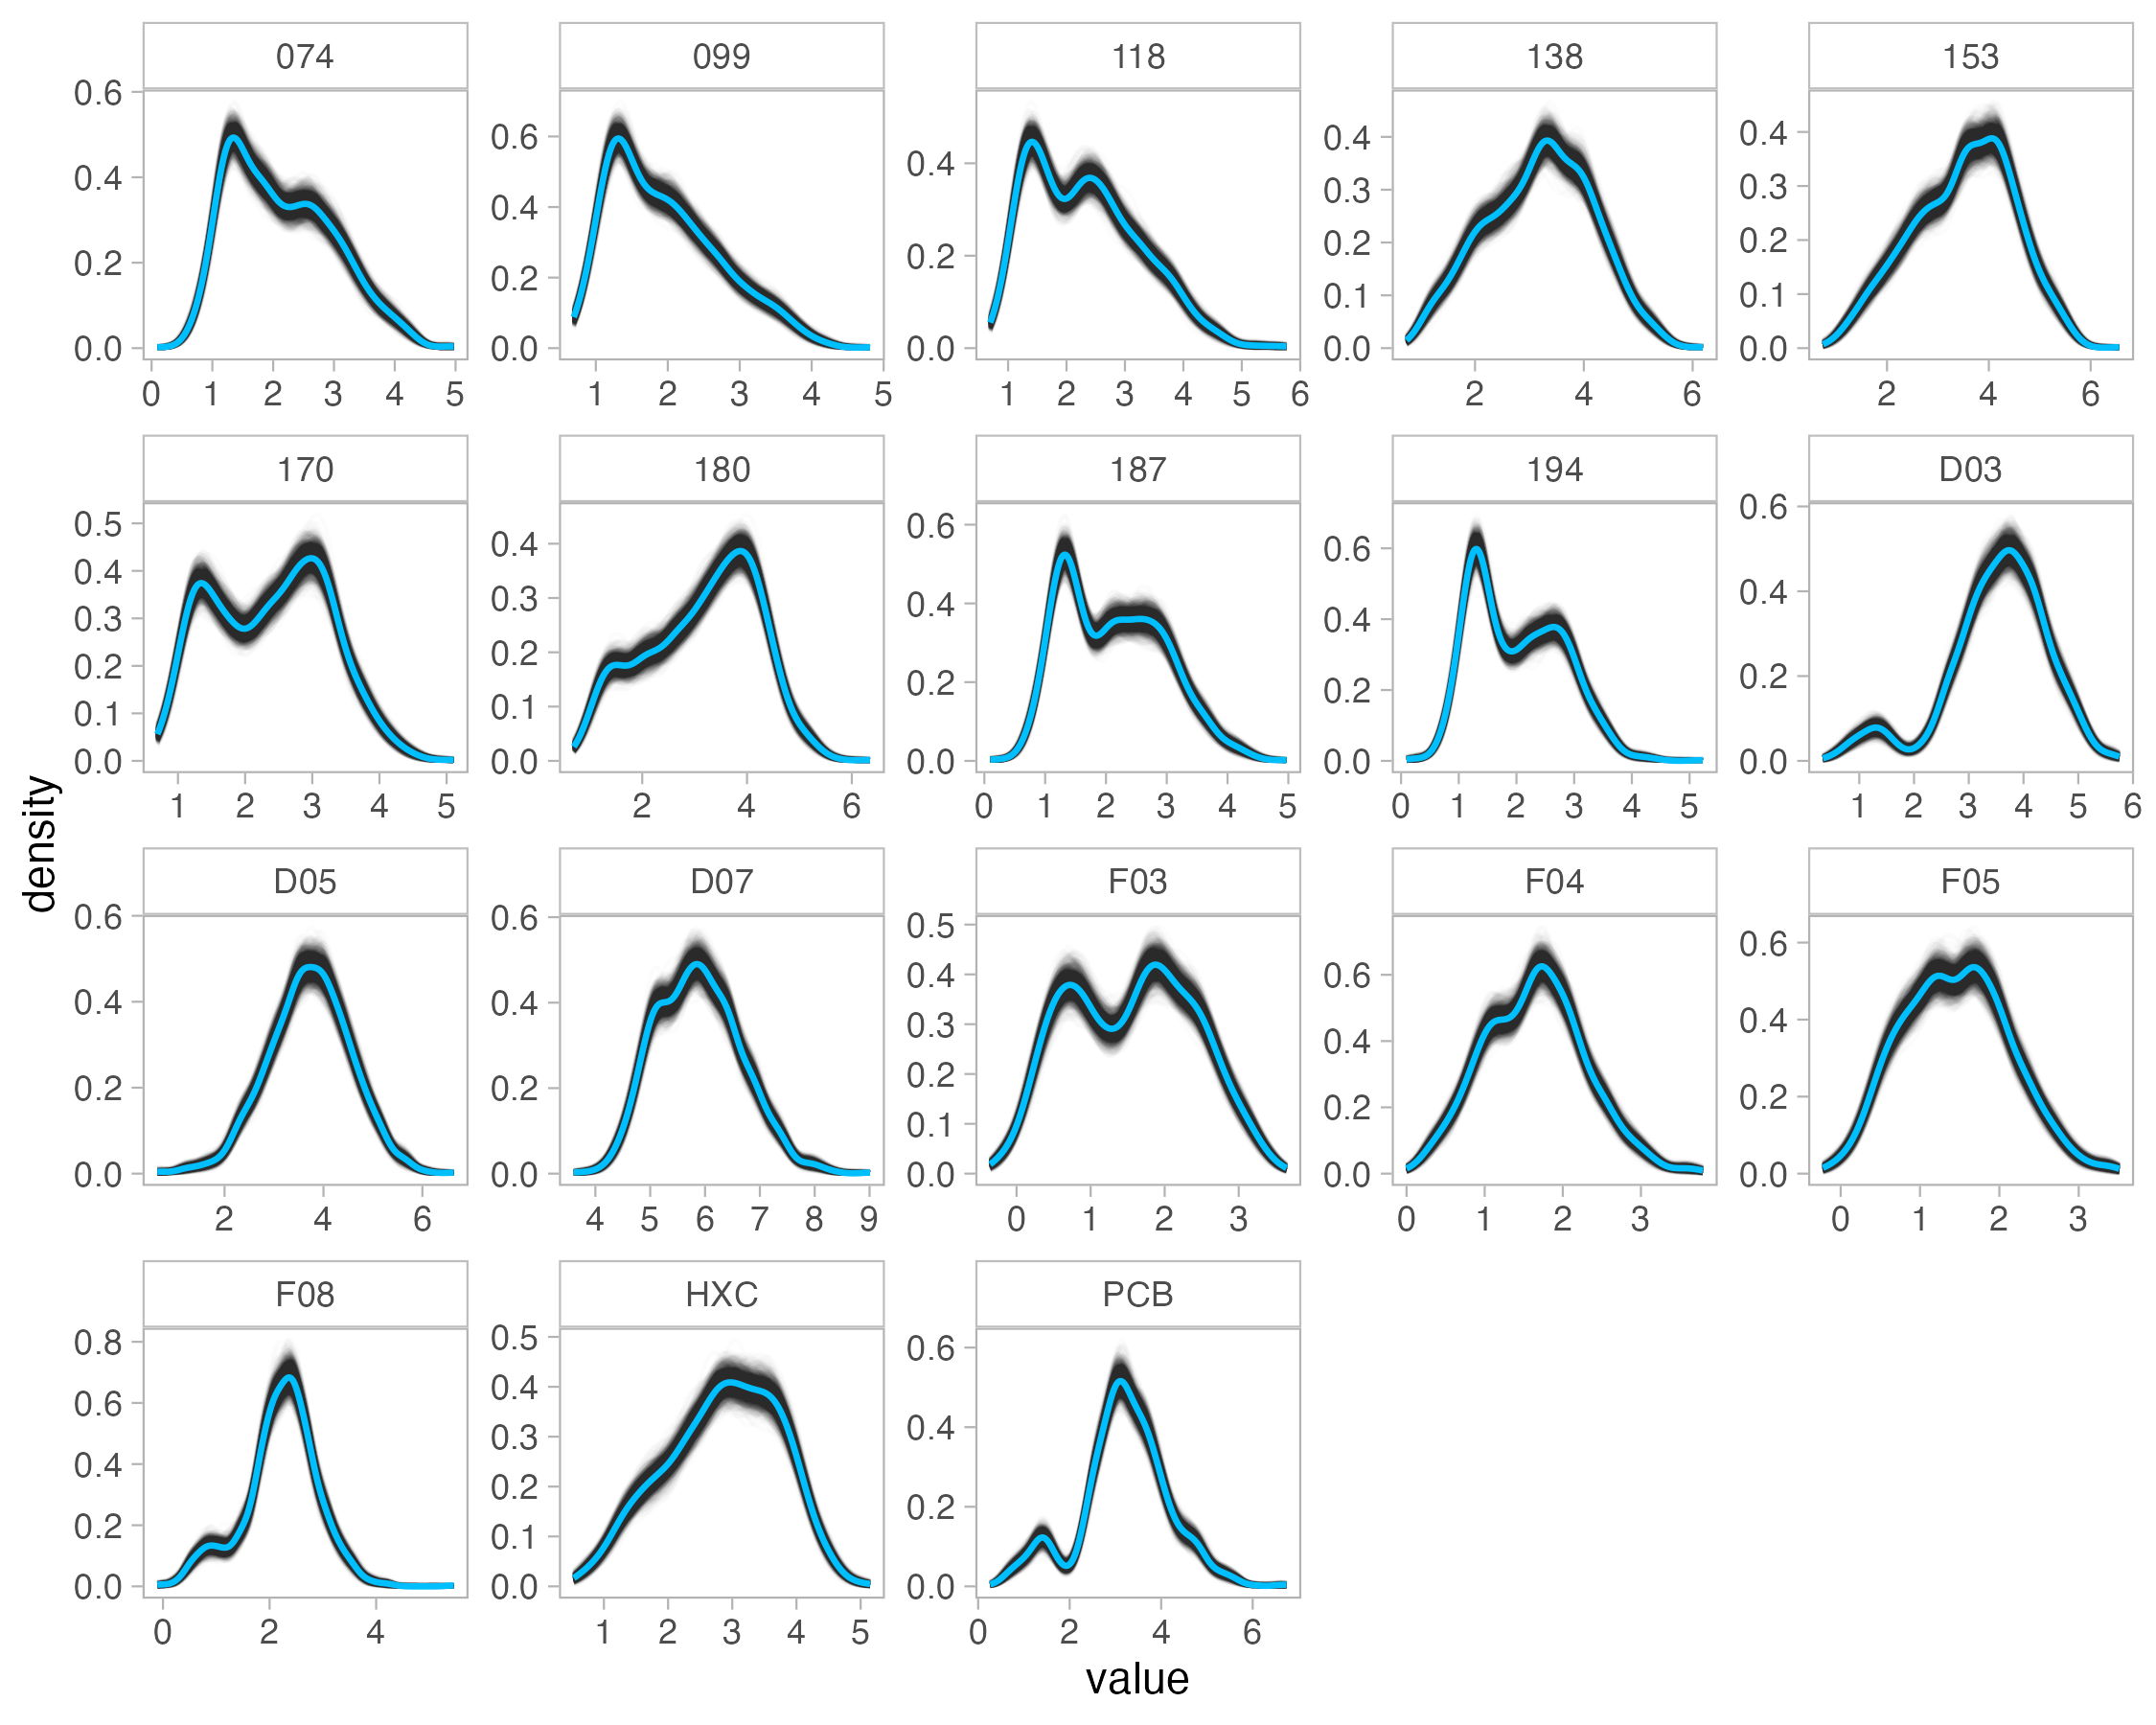
\includegraphics[width=0.75\linewidth]{figures/ch4_univ_exp_sim_lg} 

}

\caption{Distributions of exposures from observed data (blue) and simulated larger size (n=1000) datasets (gray).}\label{fig:univexplg}
\end{figure}
\begin{figure}

{\centering 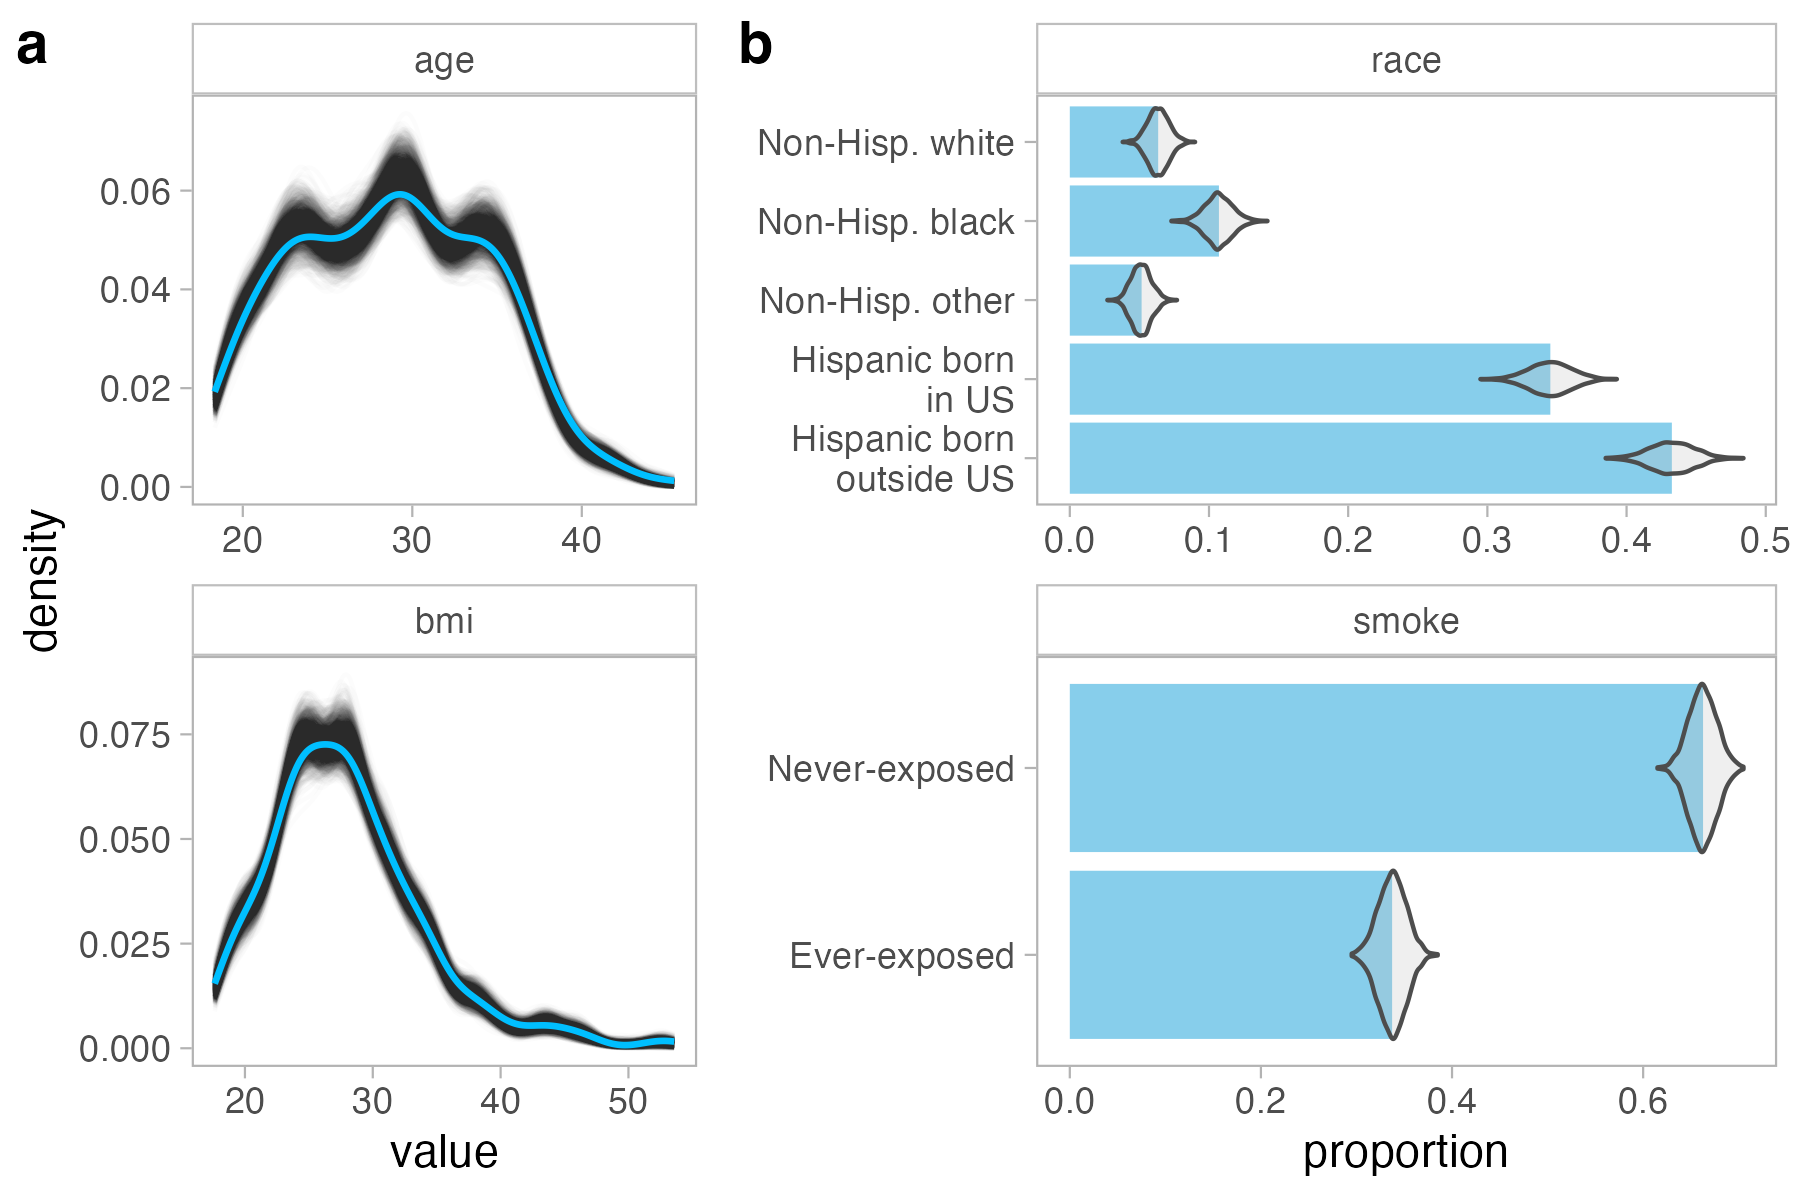
\includegraphics[width=0.75\linewidth]{figures/ch4_univ_cov_sim_lg} 

}

\caption{Distributions of covariates from observed data (blue) and simulated larger size (n=1000) datasets (gray).}\label{fig:univcovlg}
\end{figure}
\begin{figure}

{\centering 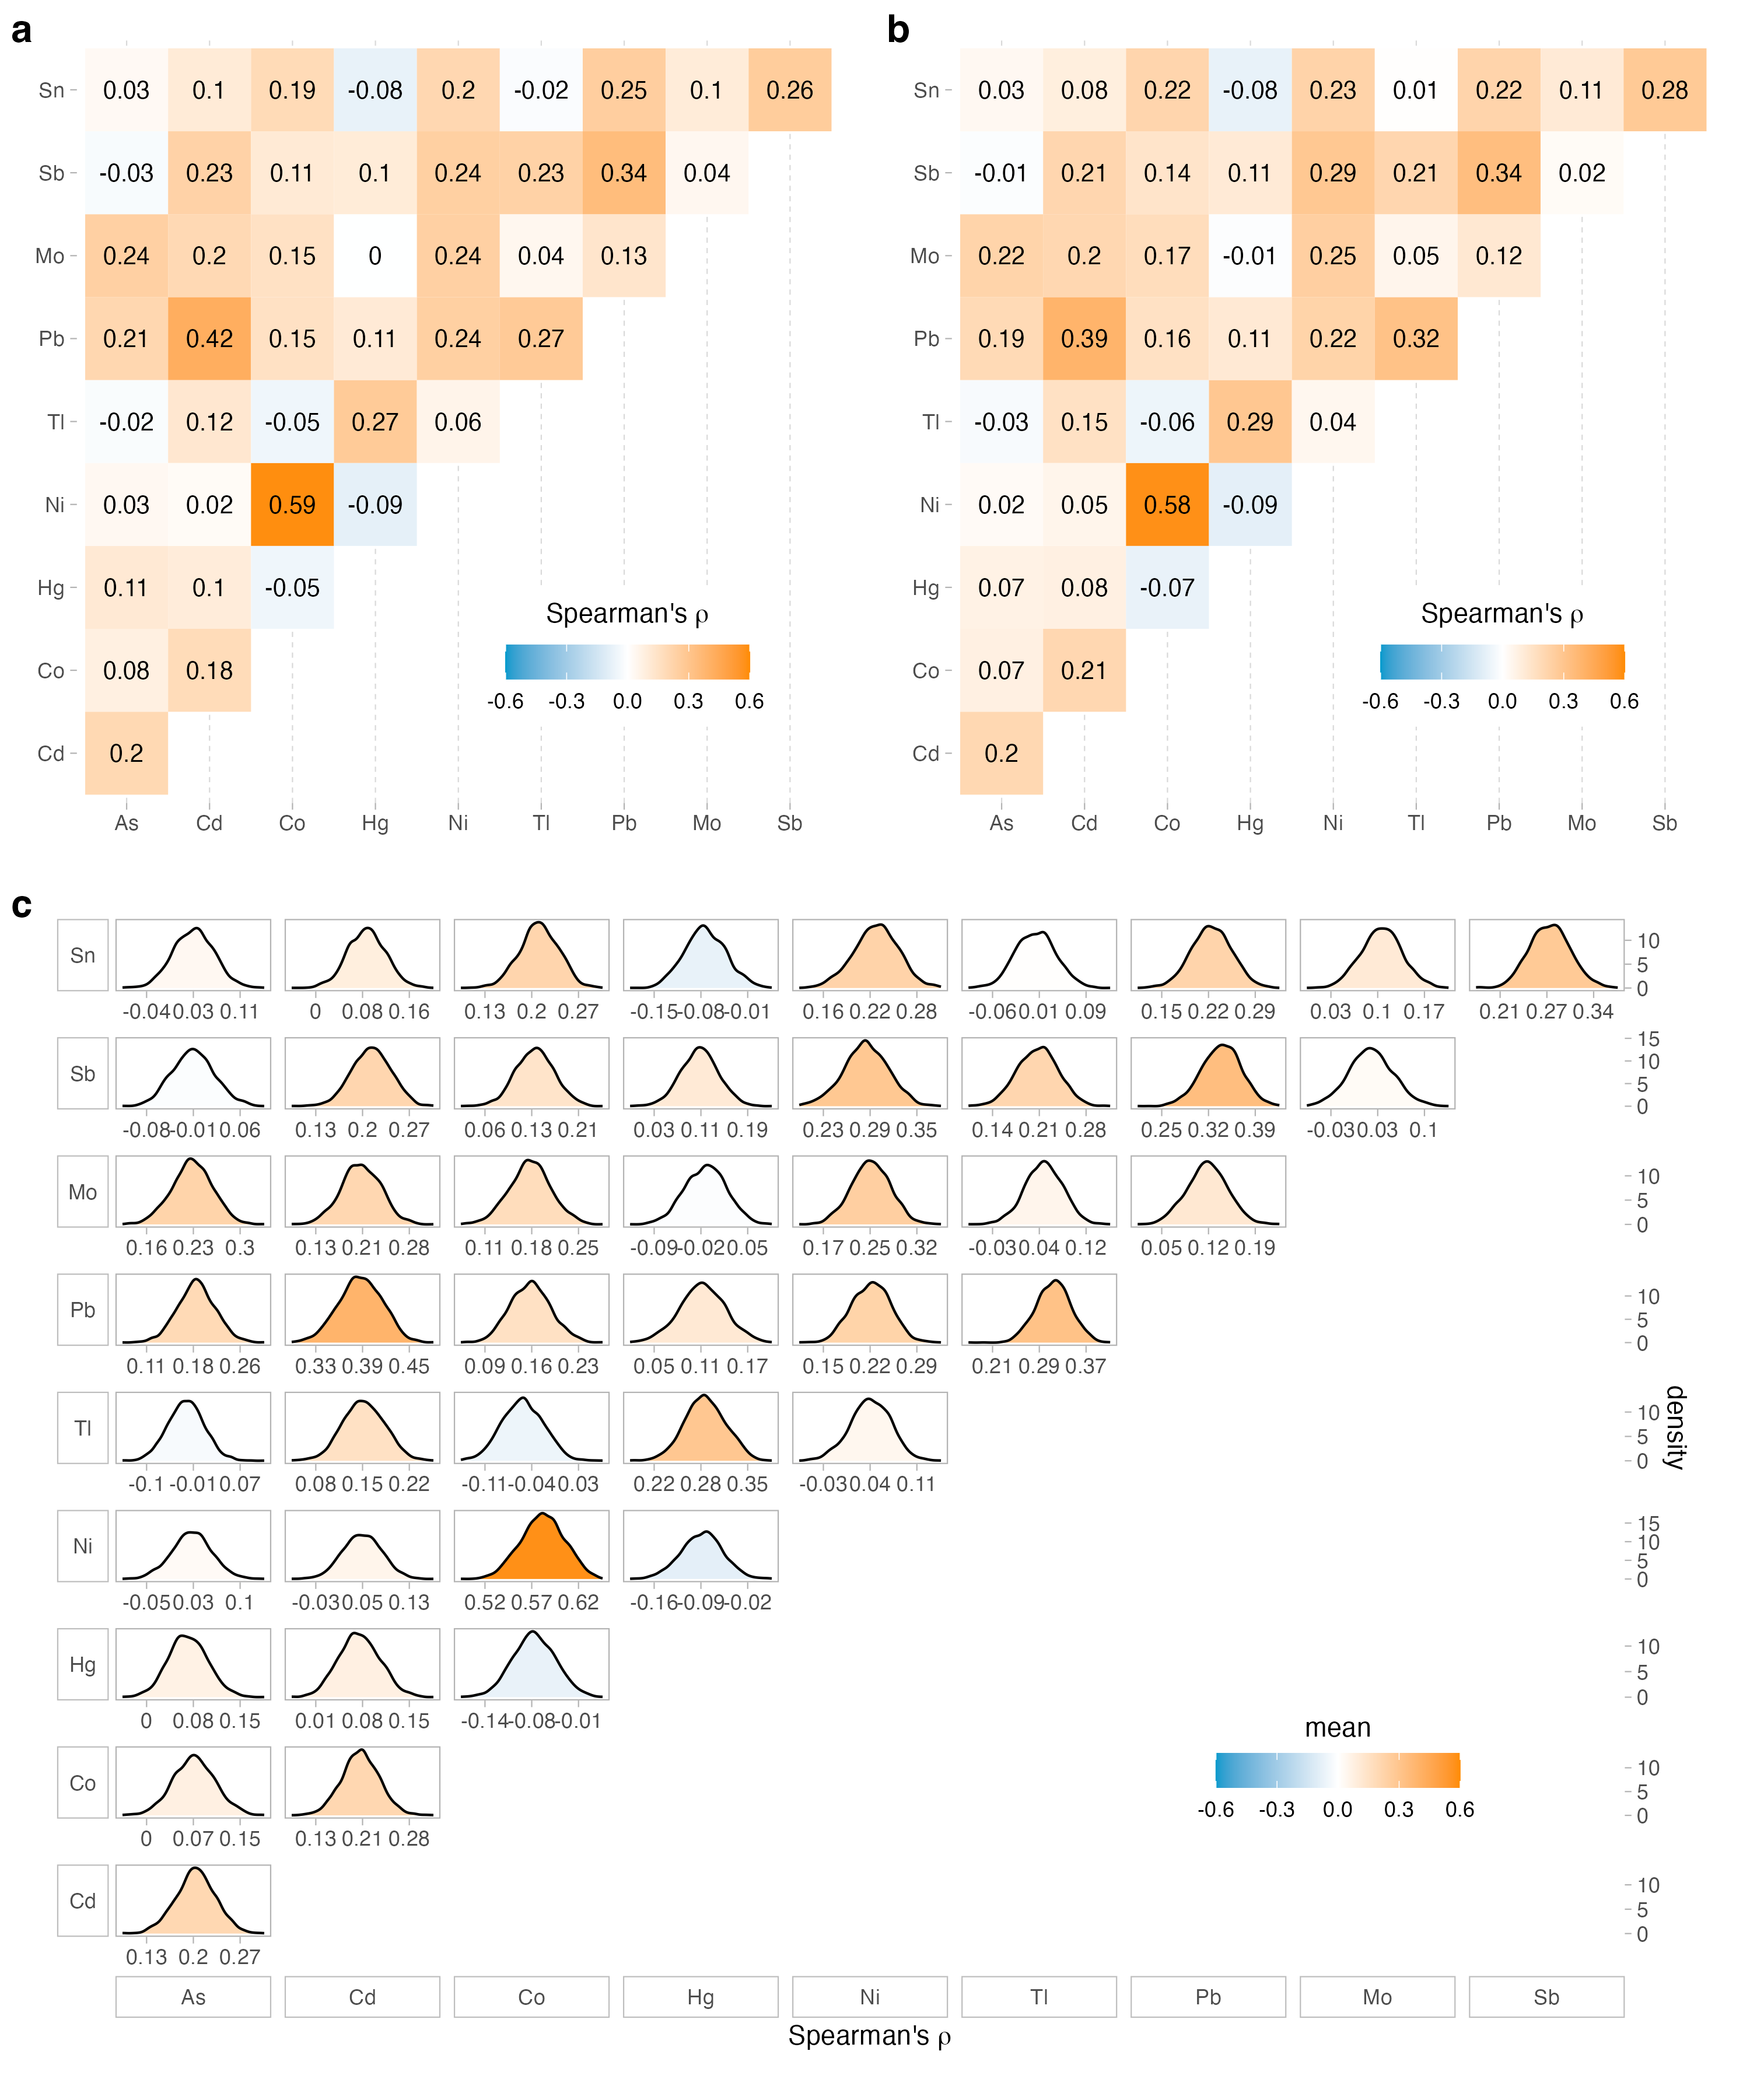
\includegraphics[width=1\linewidth]{figures/ch4_corr_lg_simorigdens} 

}

\caption{Spearman's correlation heat maps of exposures from observed data (a) and averaged from 2100 larger size (n=1000) simulated datasets (b), as well as distributions of correlations from larger size simulated datasets (c).}\label{fig:corsimslg}
\end{figure}
Figure \ref{fig:rsqcheck} visualizes the distribution of \(R^2\) values in smaller and larger size simulated datasets.
\begin{figure}

{\centering 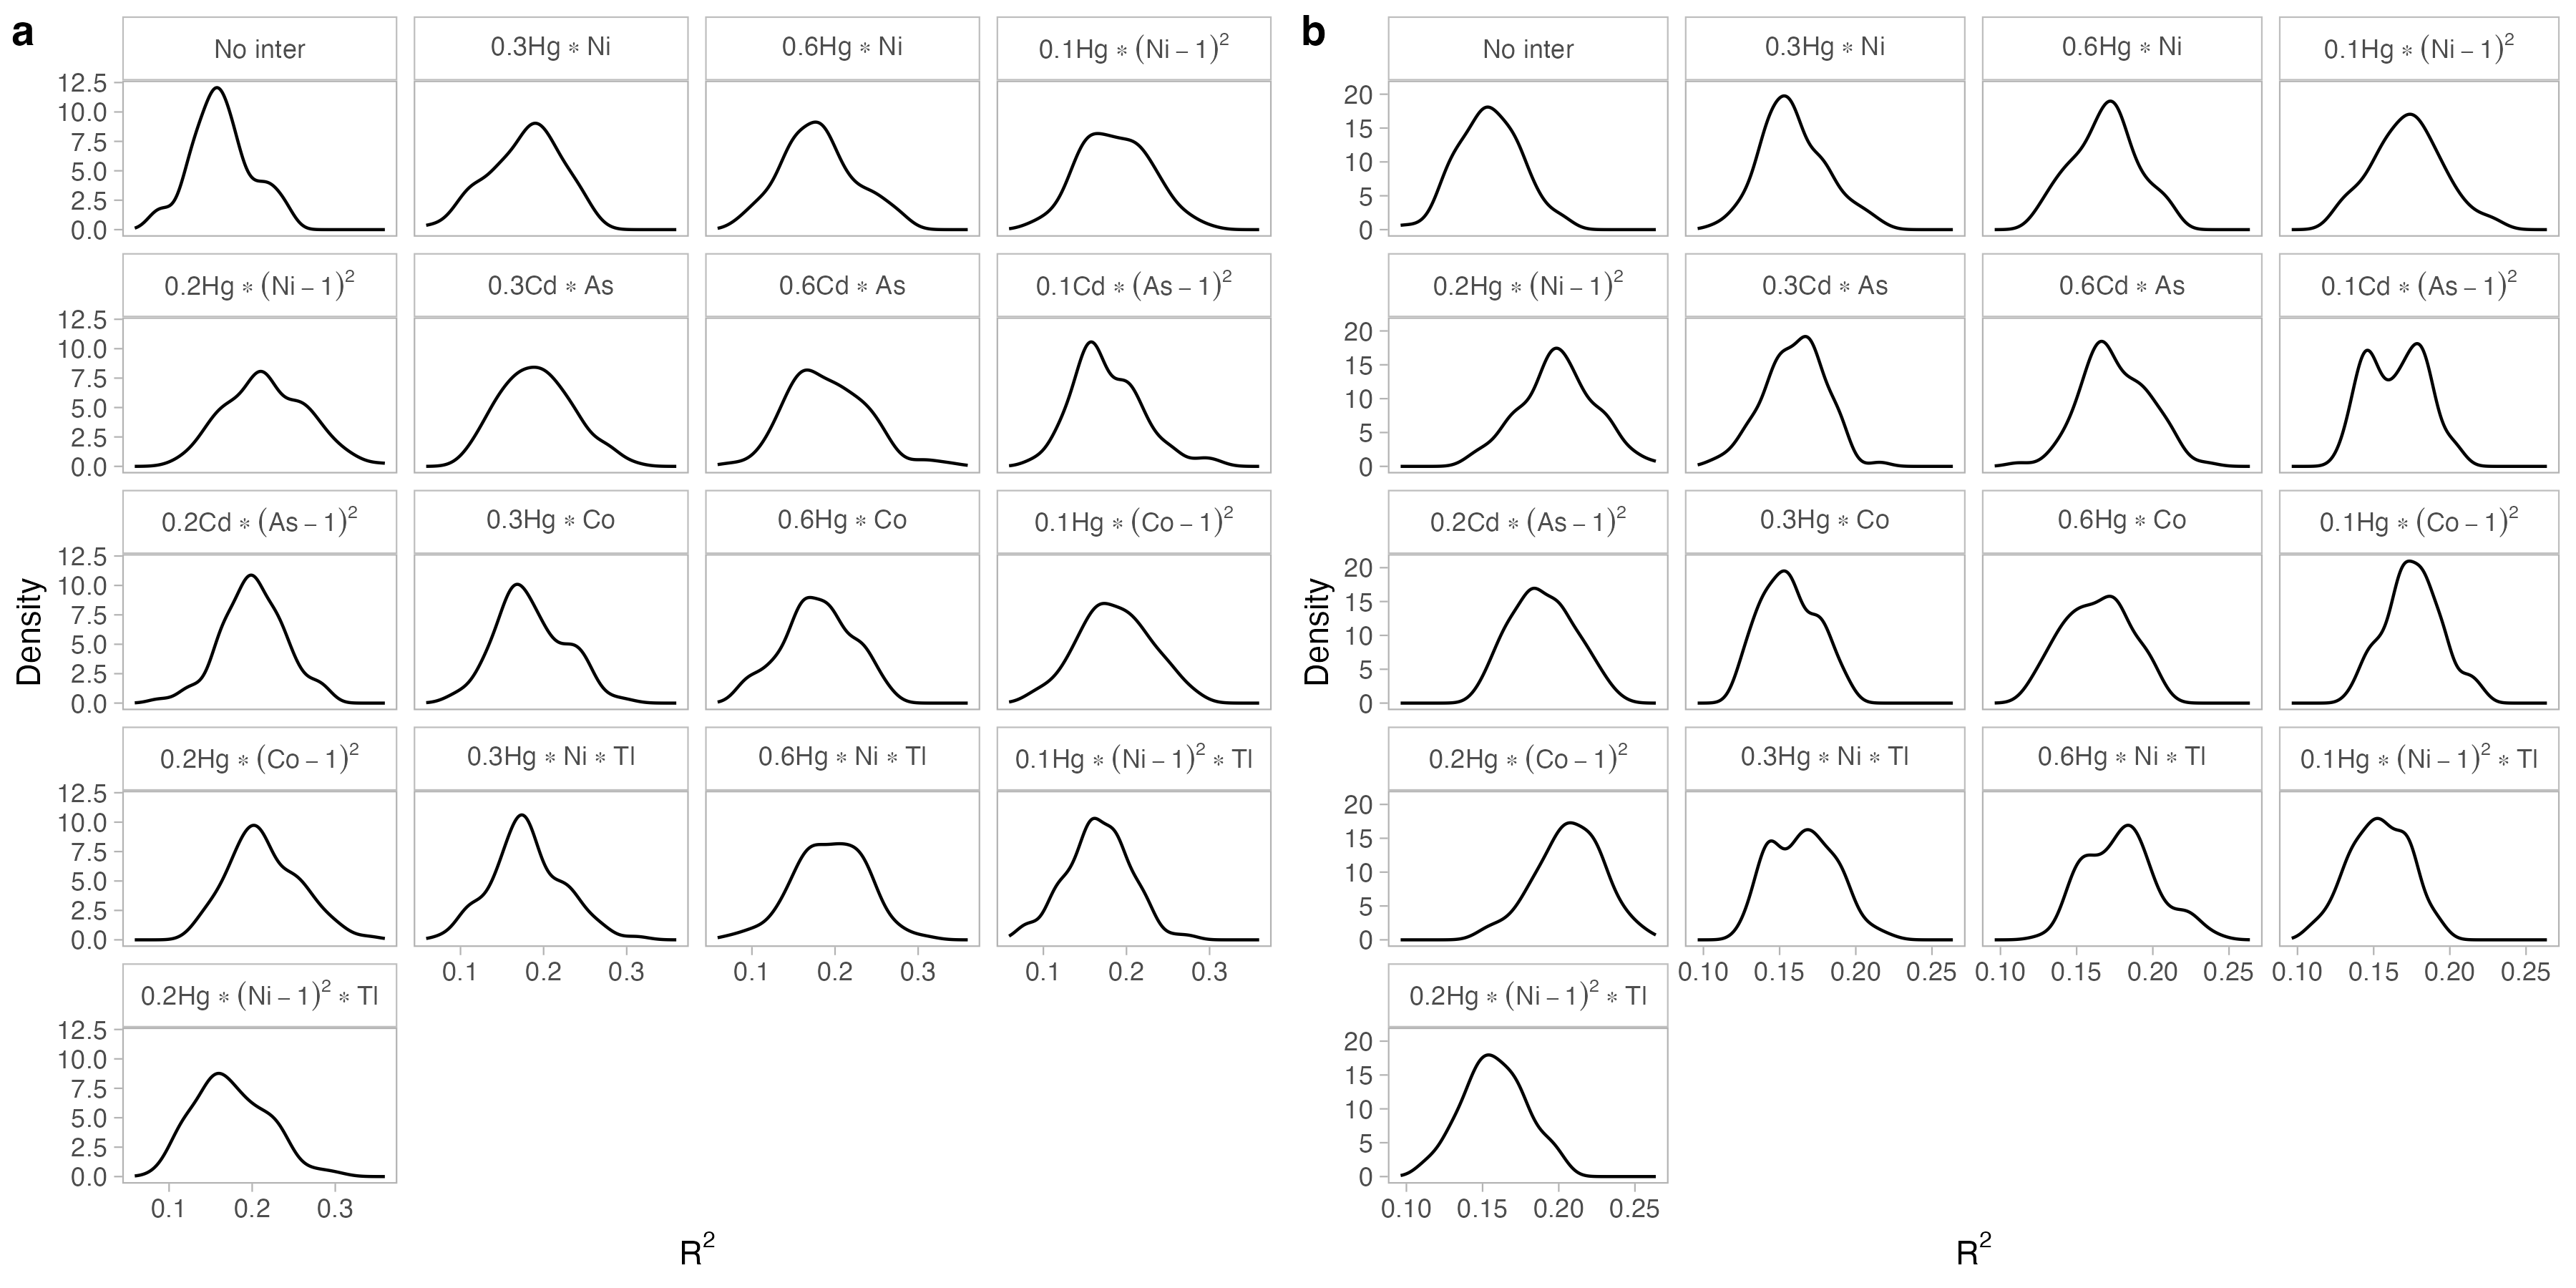
\includegraphics[width=1\linewidth]{figures/chem_rsq} 

}

\caption{R$^2$ values from multiple linear regressions with only the true functional form of significant exposures in smaller size (a) and larger size (b) simulated datasets.}\label{fig:rsqcheck}
\end{figure}
Figure \ref{fig:comparedf} compares the degrees of freedom selected using the WAIC criterion when fitting BSR using 5,000 MCMC iterations to 50,000 MCMC iterations. We ran this test on five smaller size datasets from the 16 scenarios containing interactions between exposures, as well as from the base case.
\begin{figure}

{\centering 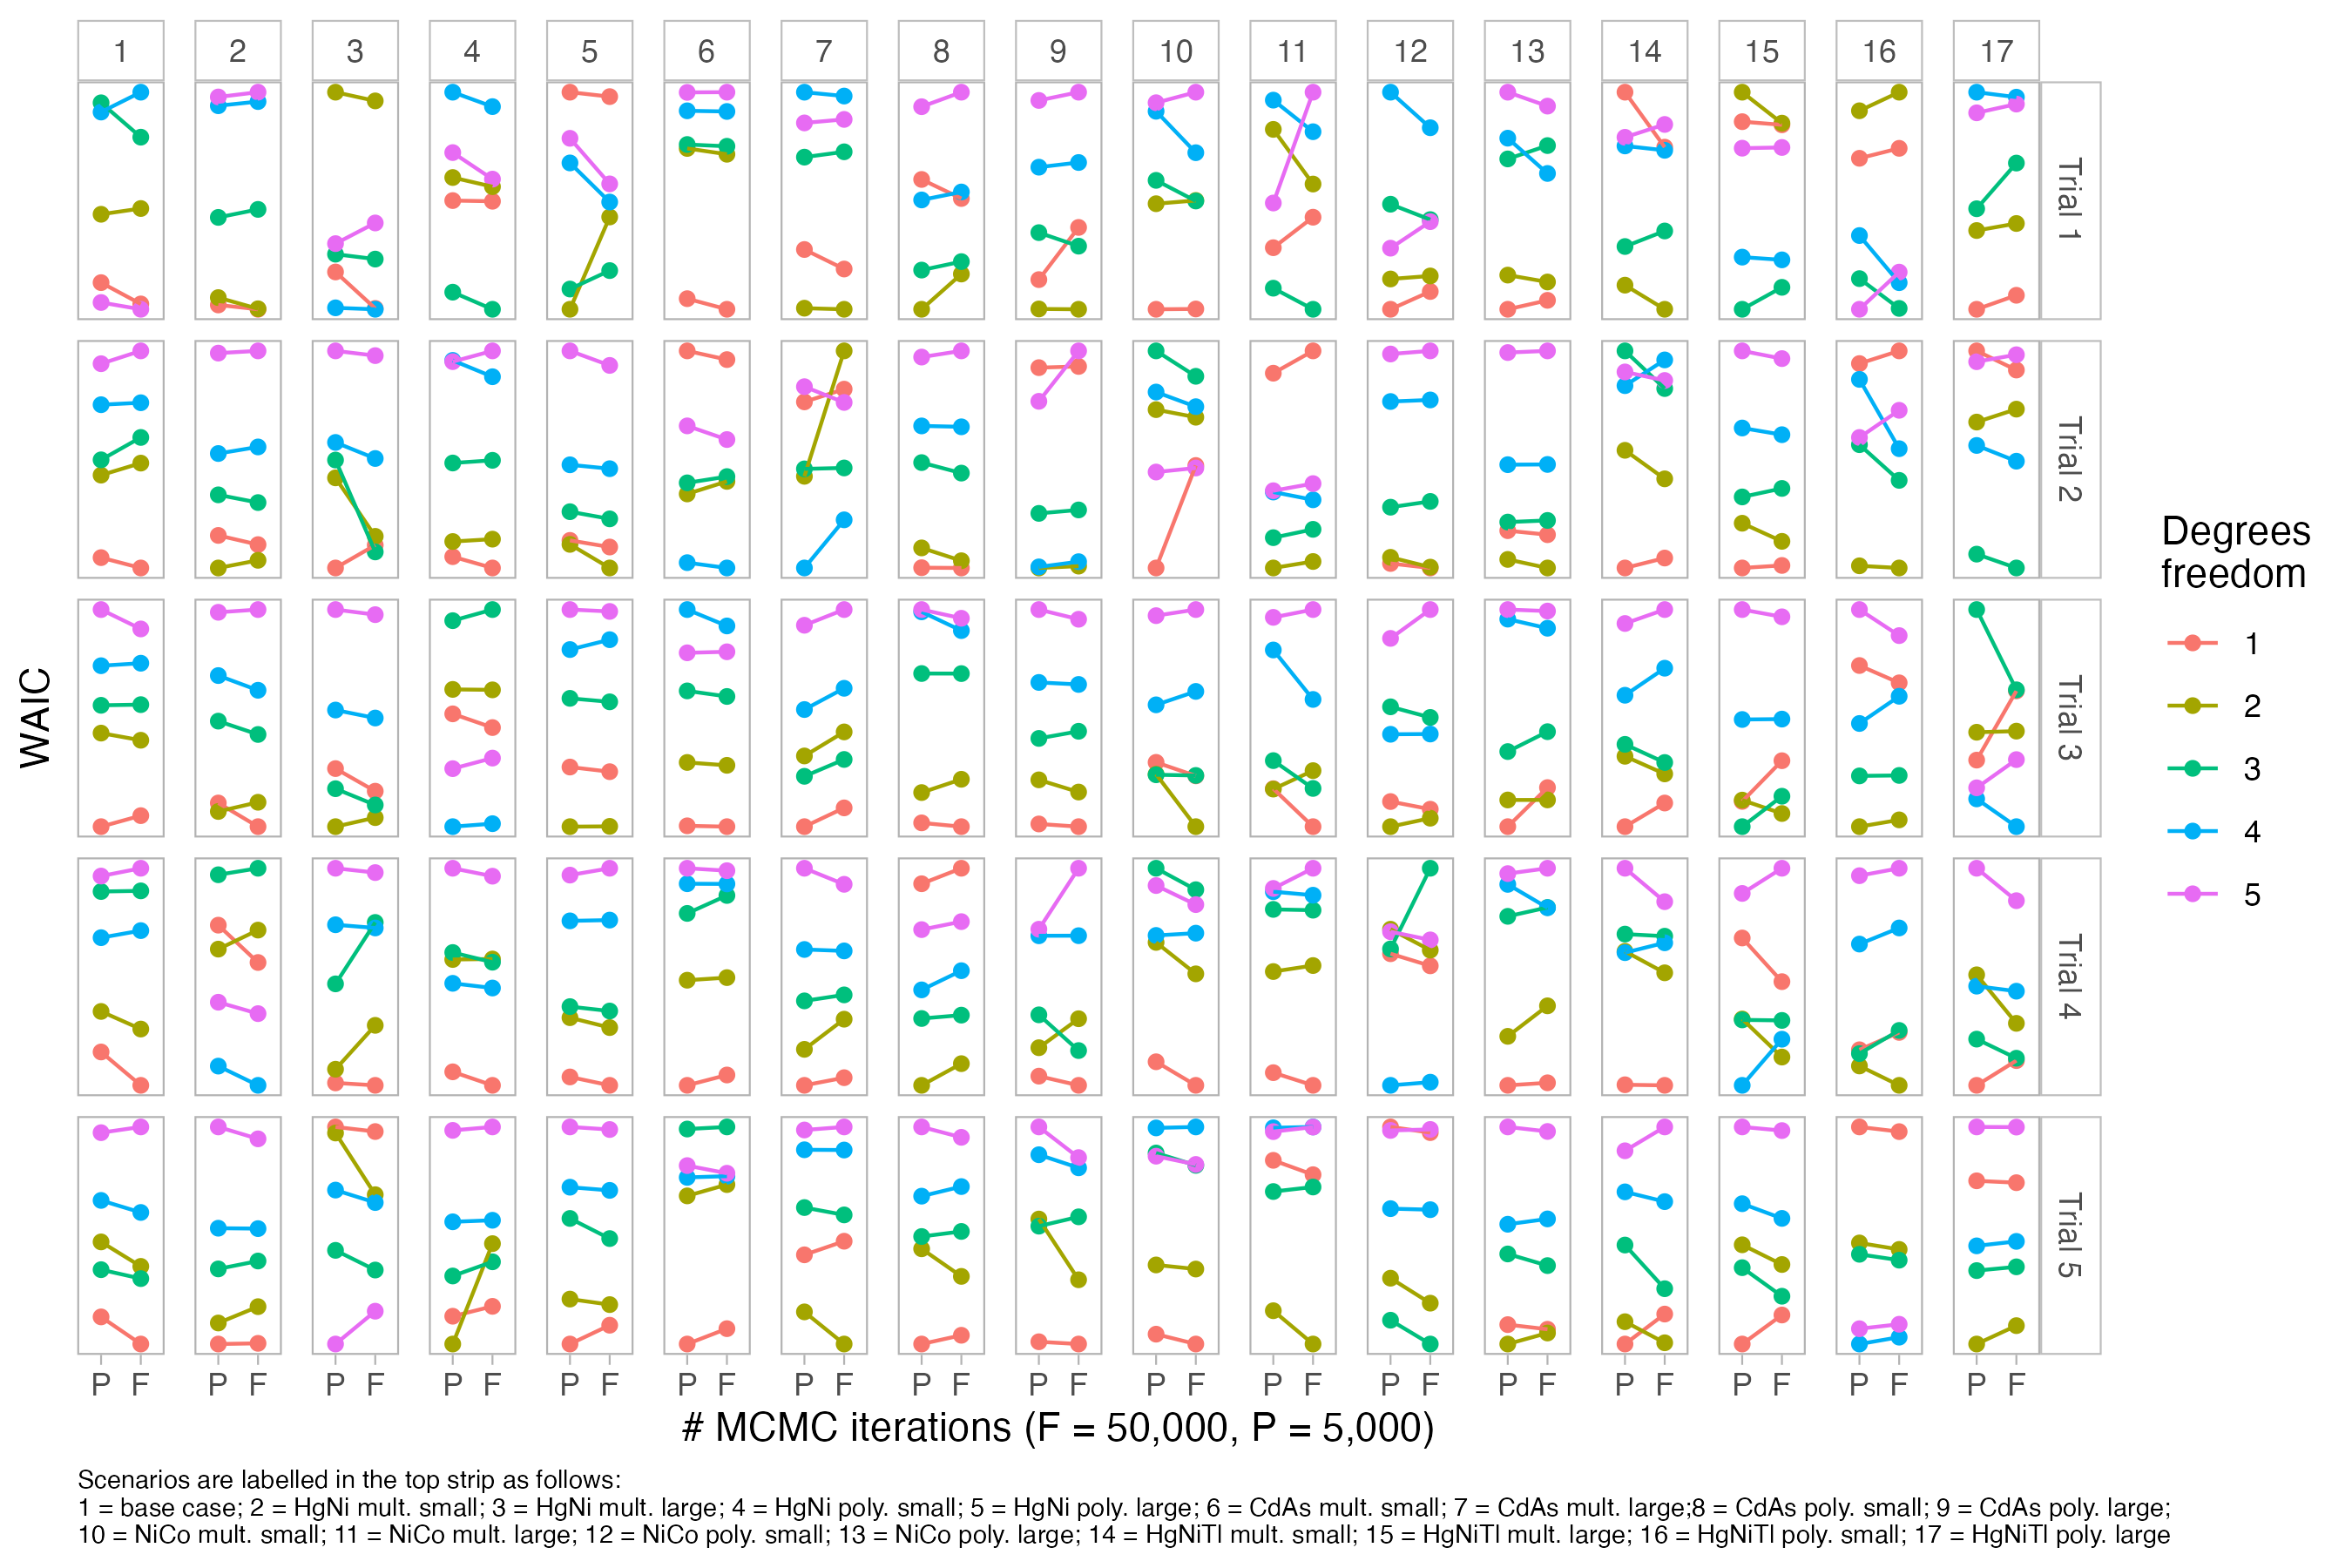
\includegraphics[width=1\linewidth]{figures/test_waic2} 

}

\caption{Test comparing WAIC selection of degrees of freedom from BSR models fit with either 5,000 or 50,000 MCMC iterations.}\label{fig:comparedf}
\end{figure}
\begin{figure}

{\centering 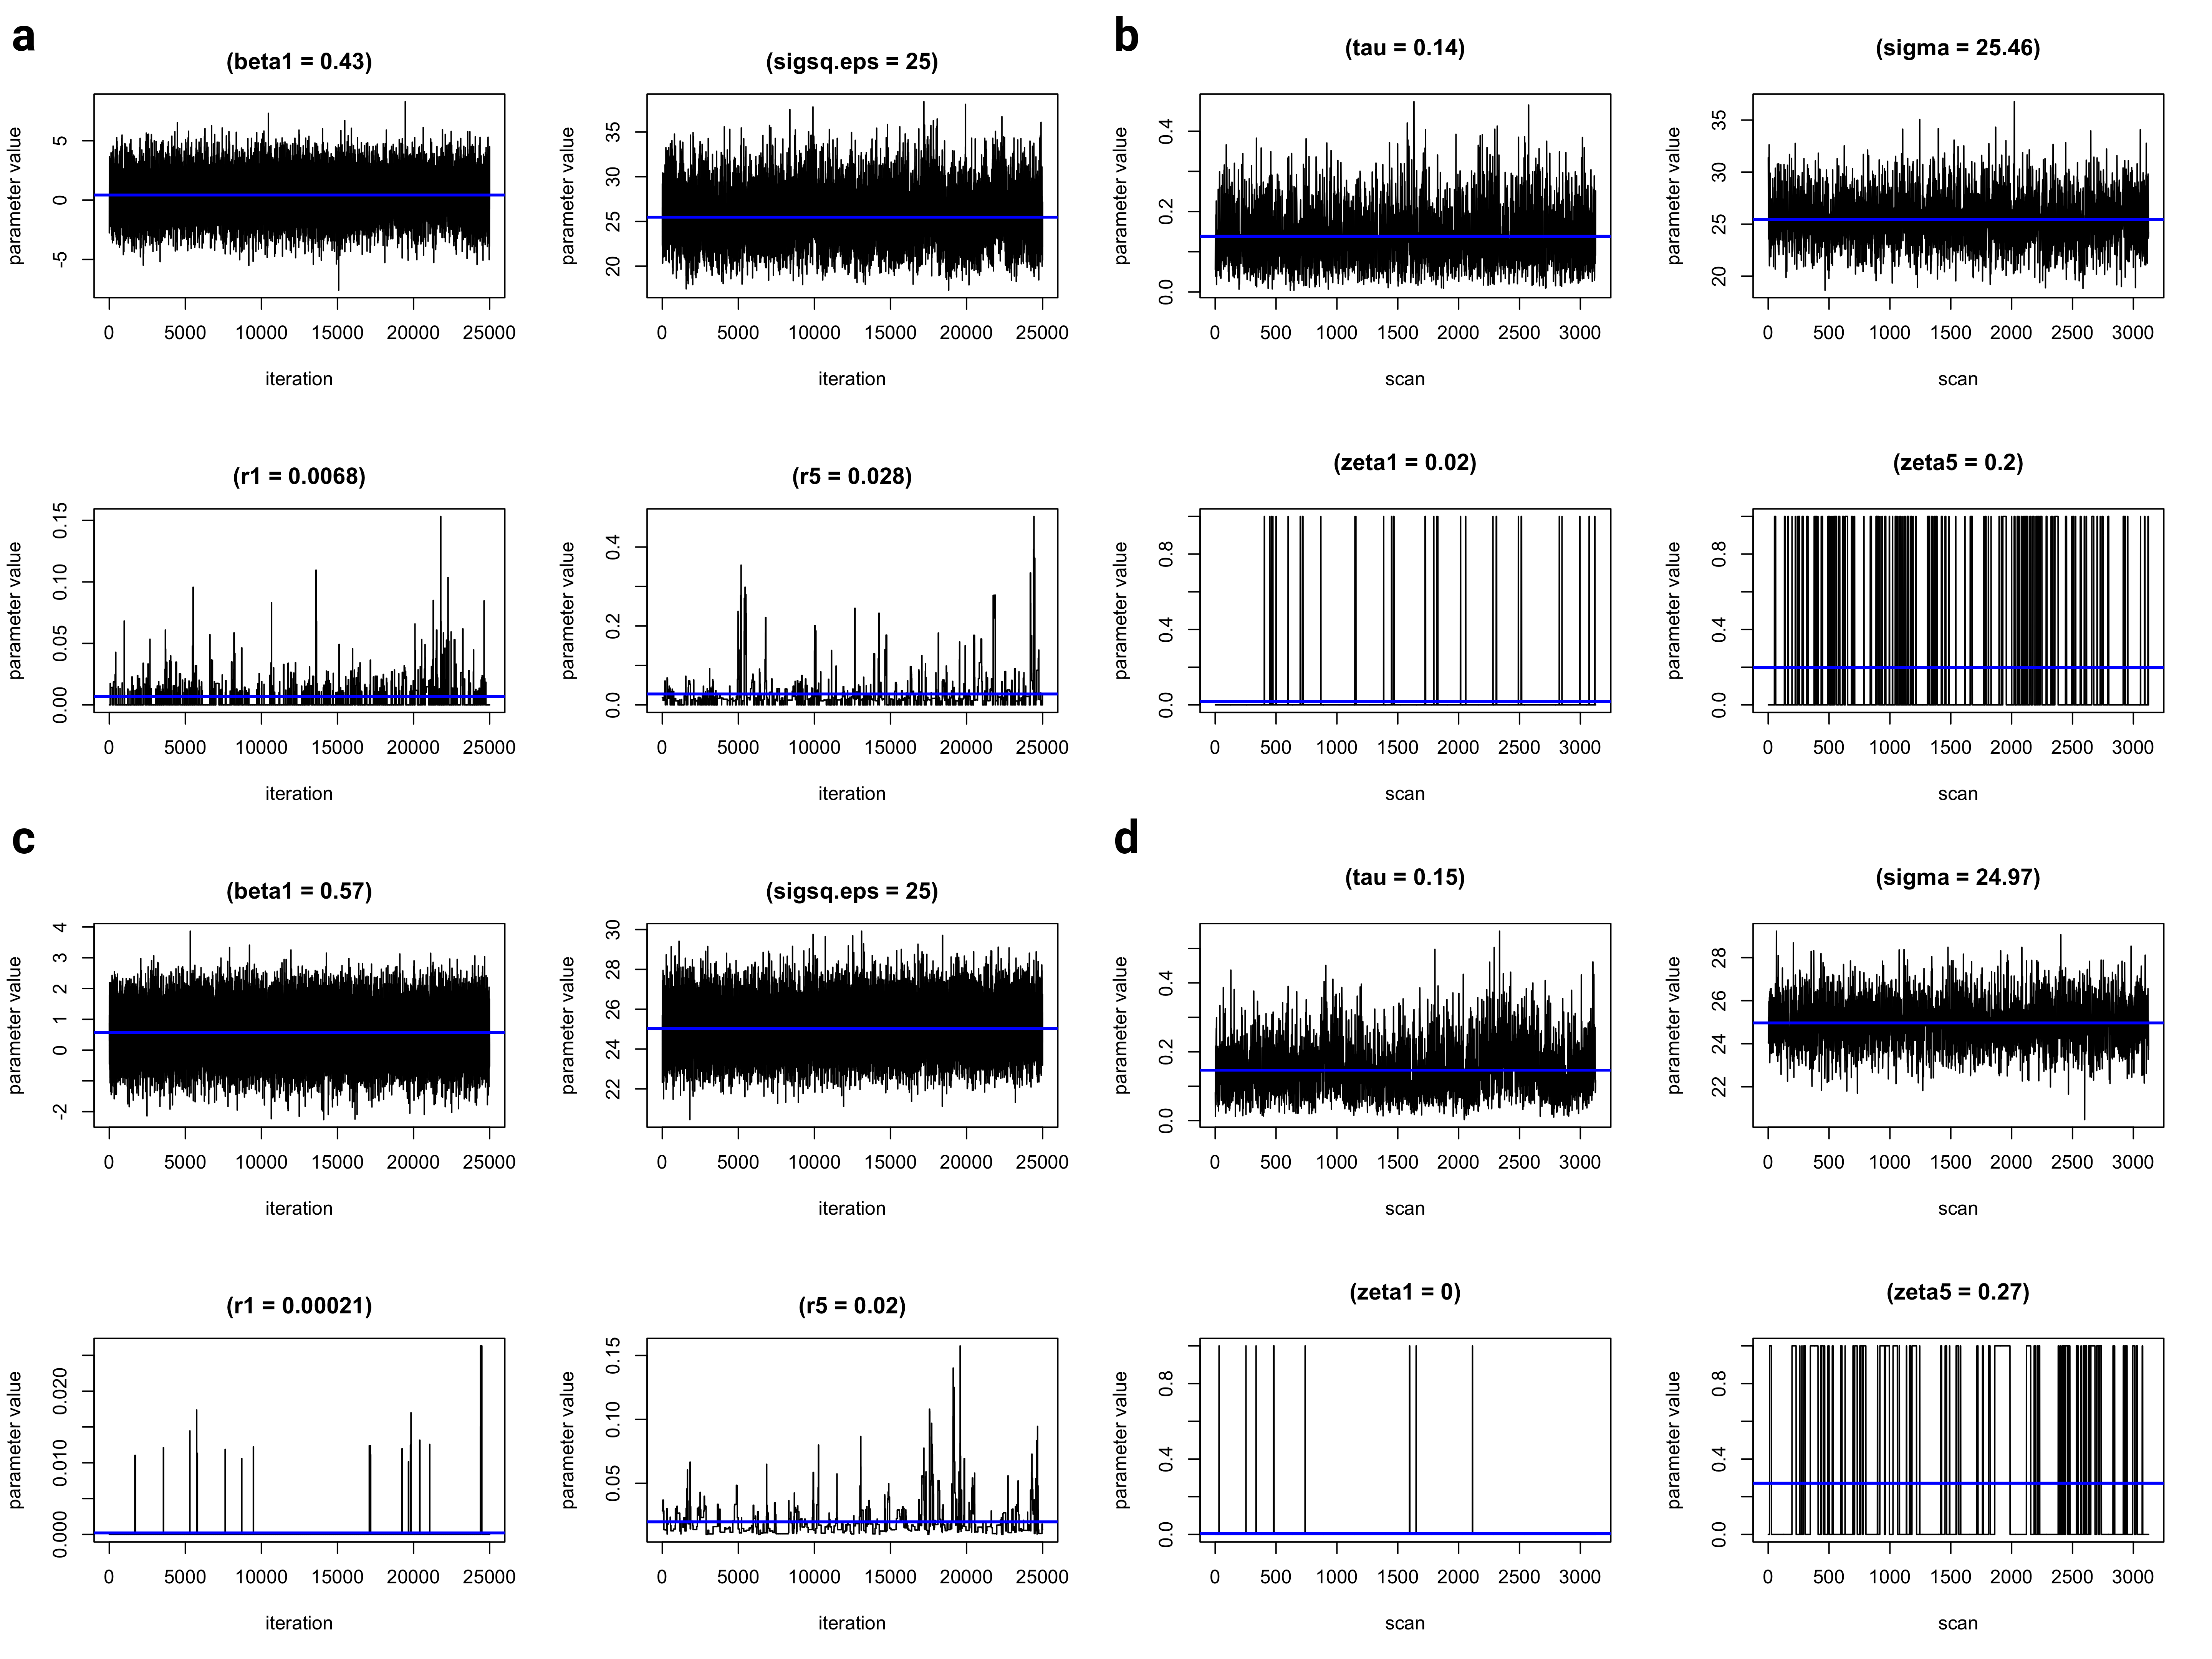
\includegraphics[width=1\linewidth]{figures/traceplots/bksm_traceplotmerged} 

}

\caption{Examples of trace plots from smaller size BKMR (a) and BSR (b) as well as larger size BKMR (c) and BSR (d) in scenarios with larger effect size interactions between Hg and Ni.}\label{fig:traceplots}
\end{figure}
Finally, we show why the order of chemicals in the confidence intervals we use to assess two-way interactions in BKMR is arbitrary. Let \(\widehat{Y}(X1_a,X2_b)\) be the estimated response at the \(a\)th quantile of \(X1\), the first chemical, the \(b\)th quantile of \(X2\), the second chemical, while holding all other chemicals at their 0.5 quantiles. Then, the estimated confidence interval of the difference in the response \(X_1\)'s 0.75 and 0.25 quantiles, at both the 0.75 and 0.25 quantiles of \(X_2\), can be shown to be equivalent to swapping the order of \(X1\) and \(X2\):
\begin{multline}
[\widehat{Y}(X1_{0.75},X2_{0.75})-\widehat{Y}(X1_{0.25},X2_{0.75})] - [\widehat{Y}(X1_{0.75},X2_{0.25})-\widehat{Y}(X1_{0.25},X2_{0.25})] \\
= \widehat{Y}(X1_{0.75},X2_{0.75})-\widehat{Y}(X1_{0.25},X2_{0.75}) - \widehat{Y}(X1_{0.75},X2_{0.25})+\widehat{Y}(X1_{0.25},X2_{0.25}) \\
= [\widehat{Y}(X1_{0.75},X2_{0.75})-\widehat{Y}(X1_{0.75},X2_{0.25})] - [\widehat{Y}(X1_{0.25},X2_{0.75})-\widehat{Y}(X1_{0.25},X2_{0.25})] \\
= \widehat{Y}(X1_{0.75},X2_{0.75})- \widehat{Y}(X1_{0.75},X2_{0.25})
-\widehat{Y}(X1_{0.25},X2_{0.75}) +\widehat{Y}(X1_{0.25},X2_{0.25}).
  \label{eq:confinteq}
\end{multline}
\hypertarget{suppresults}{%
\section{Results}\label{suppresults}}

Figures \ref{fig:nsmunivp}-\ref{fig:slgunivp} display the full distributions of univariate p-values and PIPs for all models in scenarios with interactions between chemicals that were not included in Chapter \ref{univsenschap}.
\begin{figure}

{\centering 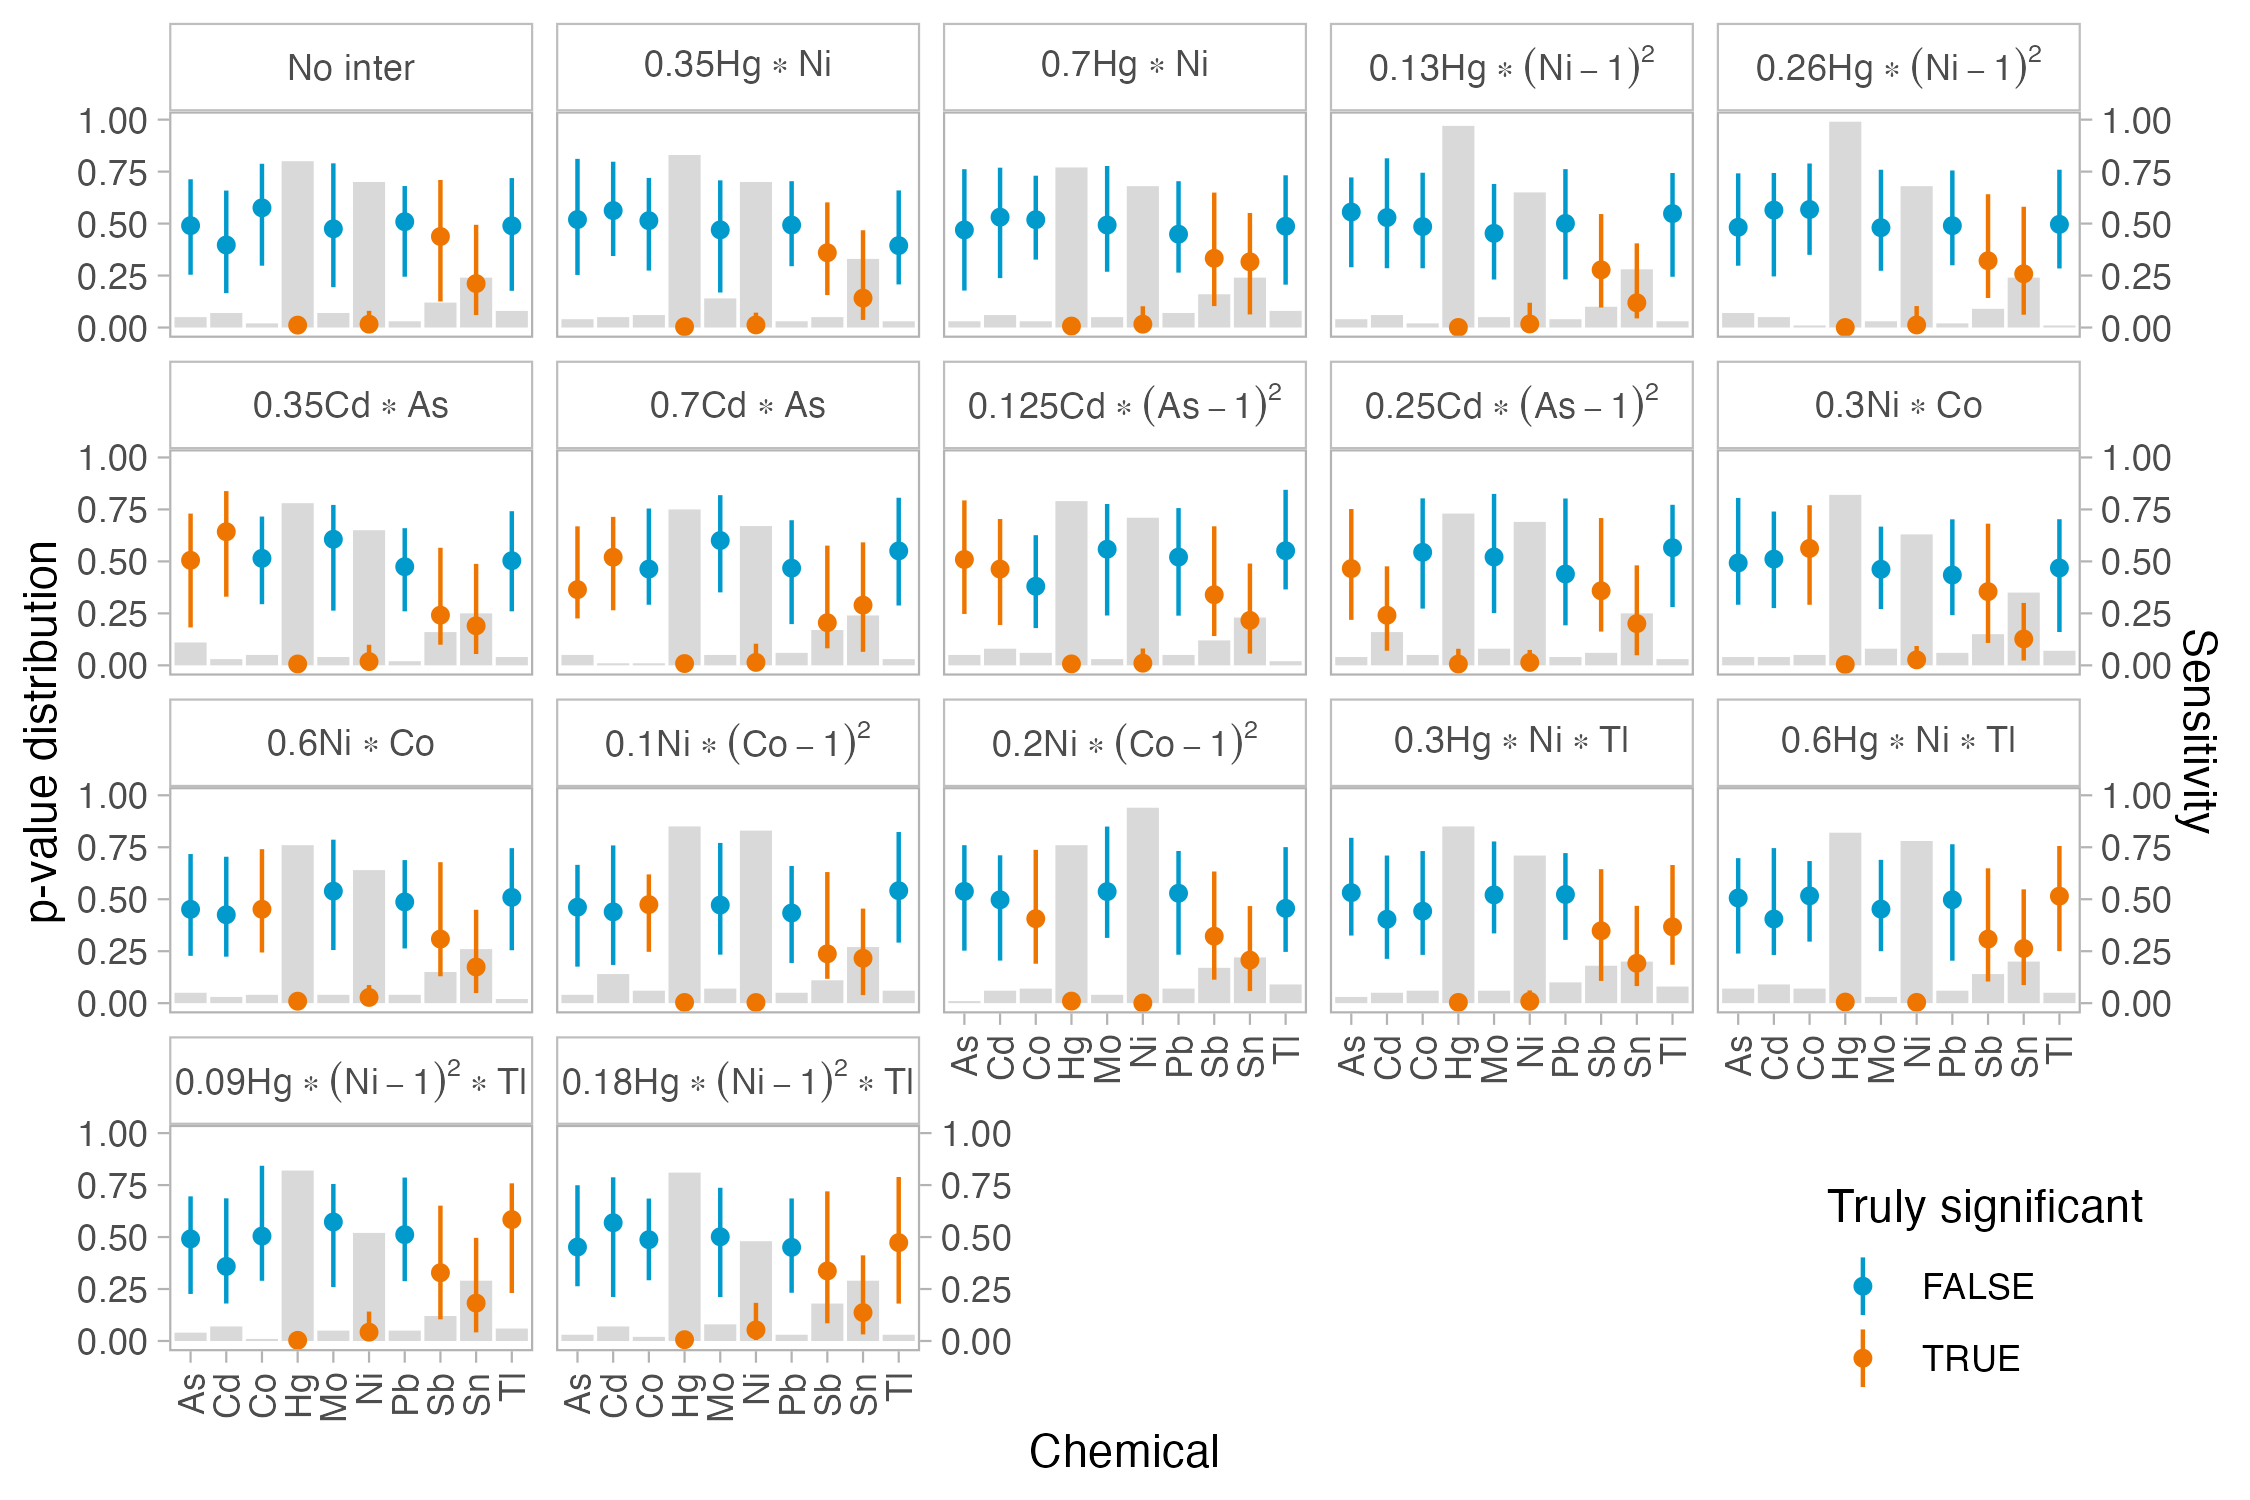
\includegraphics[width=0.8\linewidth]{figures/ch4_nsm_univ_pval} 

}

\caption{P-value distributions of univariate chemicals from naive MLRs run on smaller size (n=252) datasets, in all scenarios with interactions between chemicals. Detection rates are displayed above a point-range with the median and first and third quartiles.}\label{fig:nsmunivp}
\end{figure}
\begin{figure}

{\centering 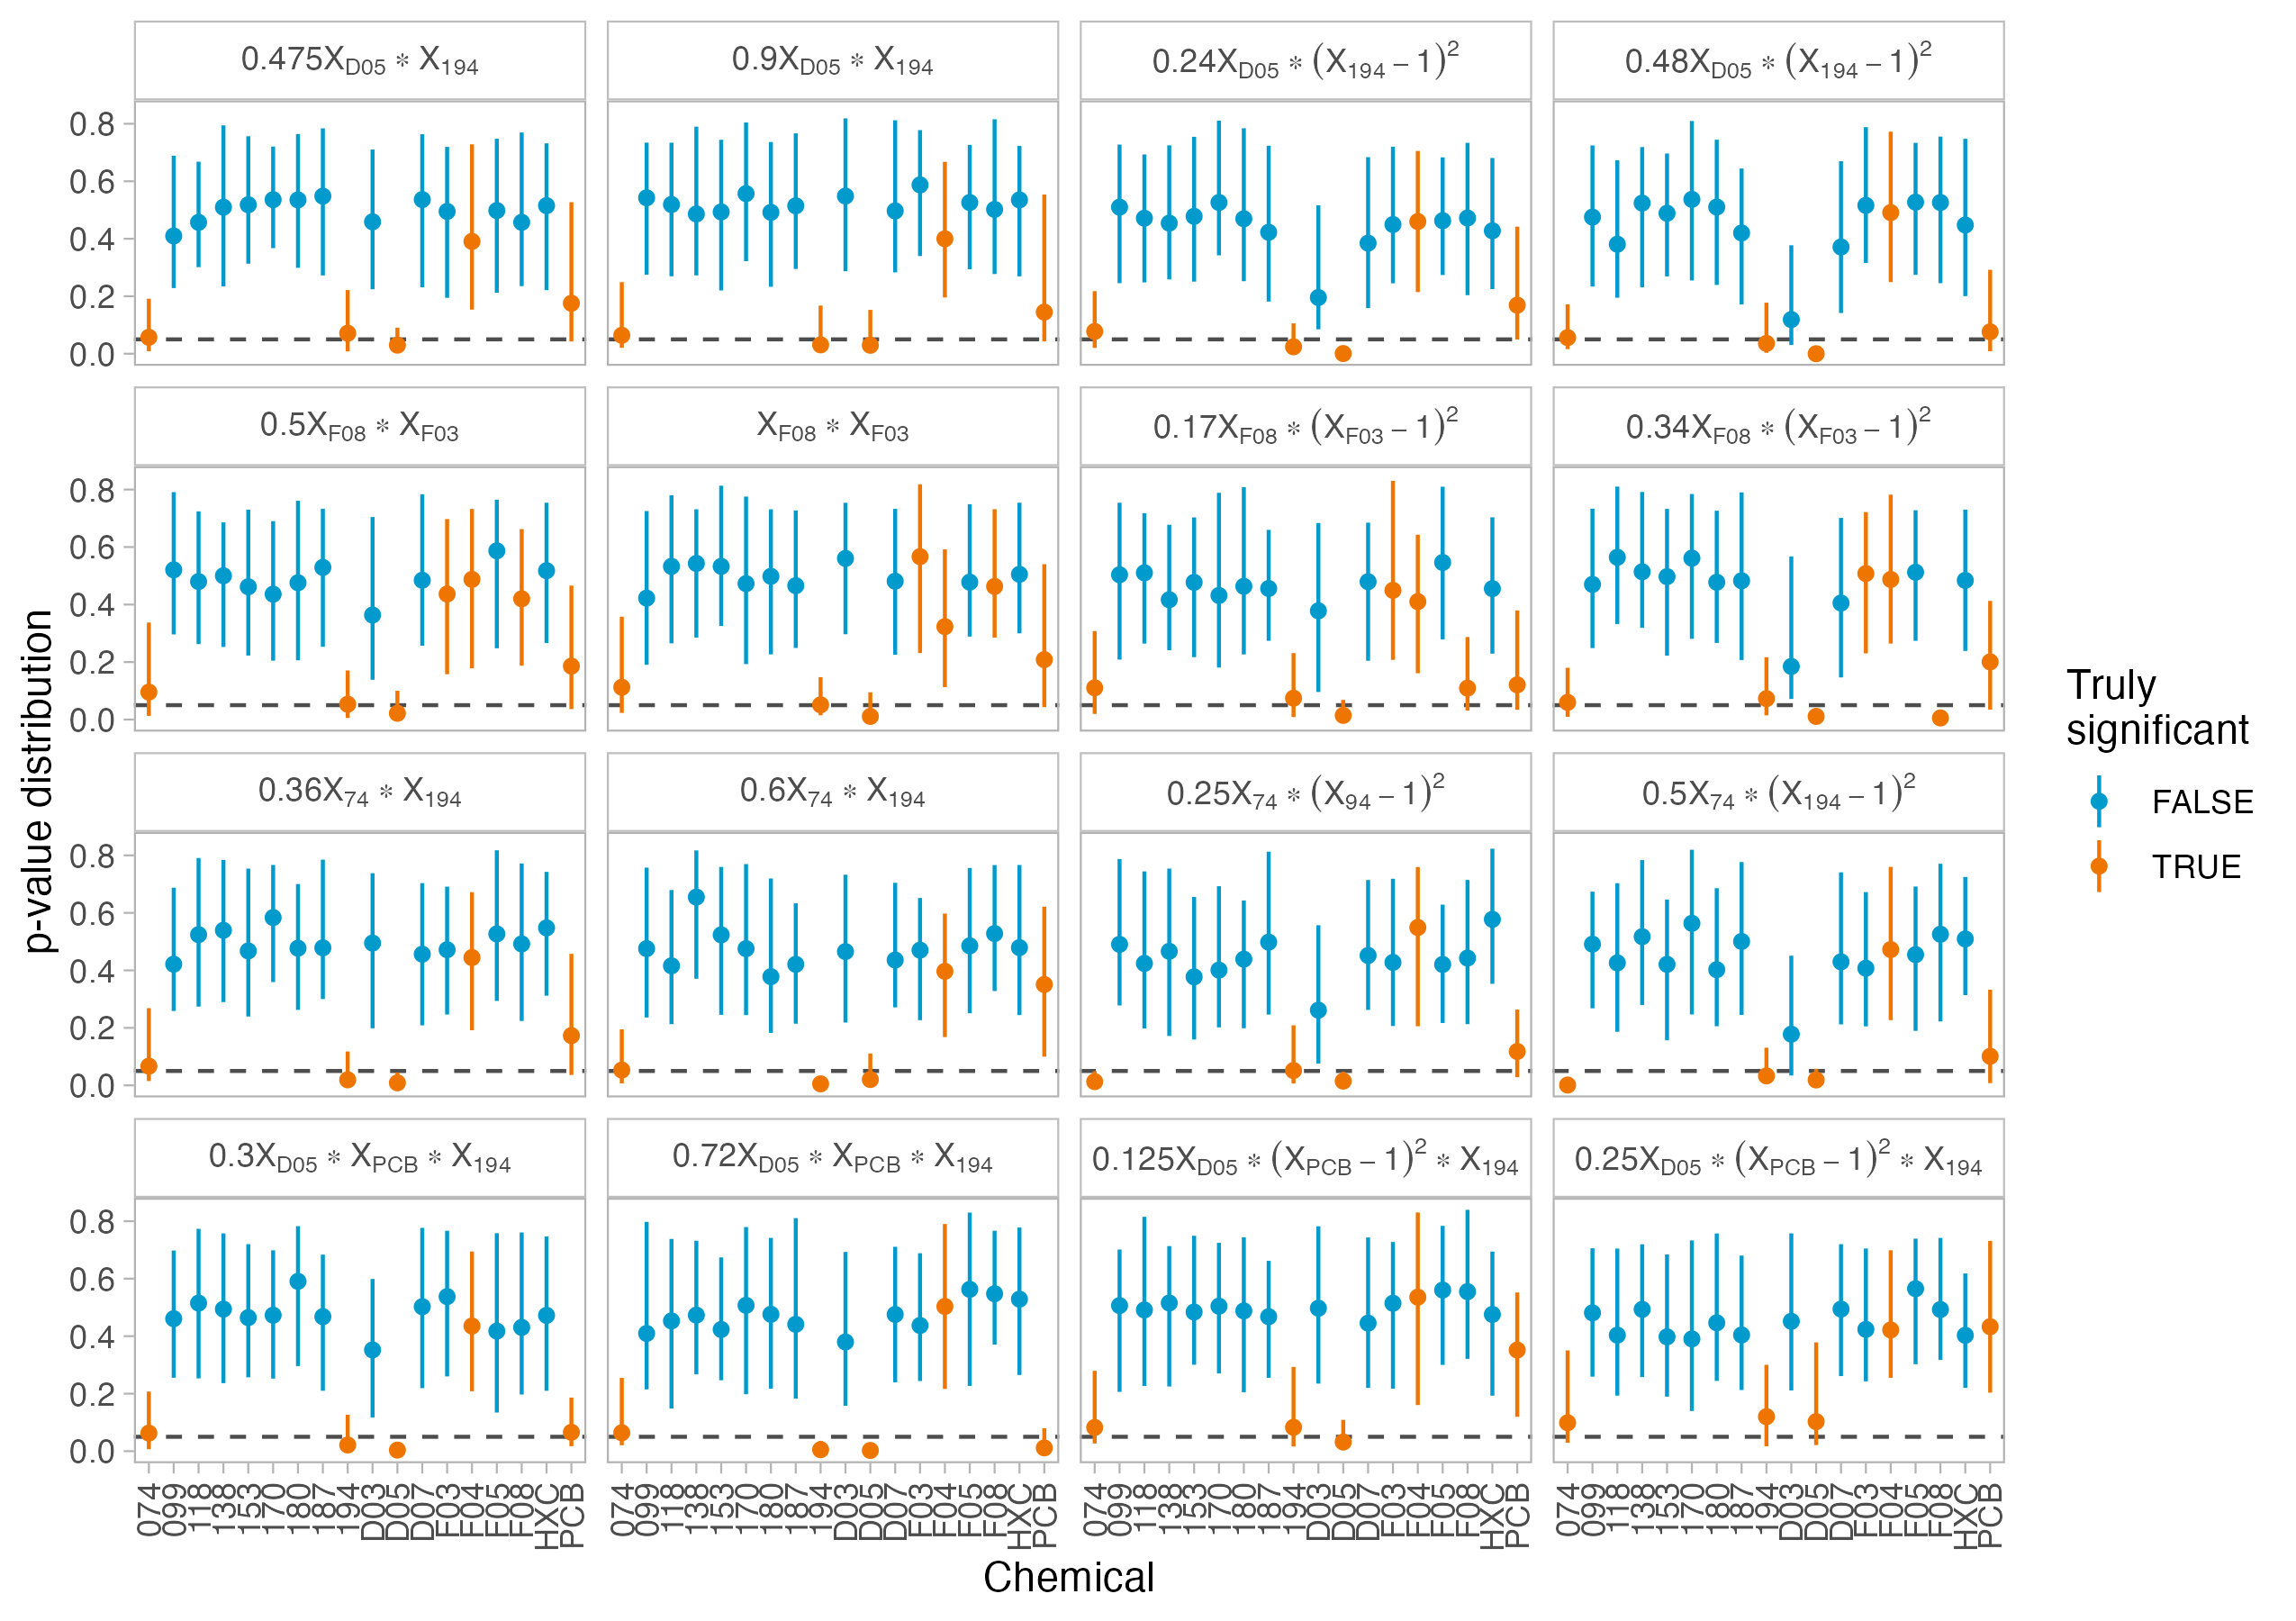
\includegraphics[width=0.8\linewidth]{figures/ch4_nlg_univ_pval} 

}

\caption{P-value distributions of univariate chemicals from naive MLRs run on larger size (n=1000) datasets, in all scenarios with interactions between chemicals. Detection rates are displayed above a point-range with the median and first and third quartiles.}\label{fig:nlgunivp}
\end{figure}
\begin{figure}

{\centering 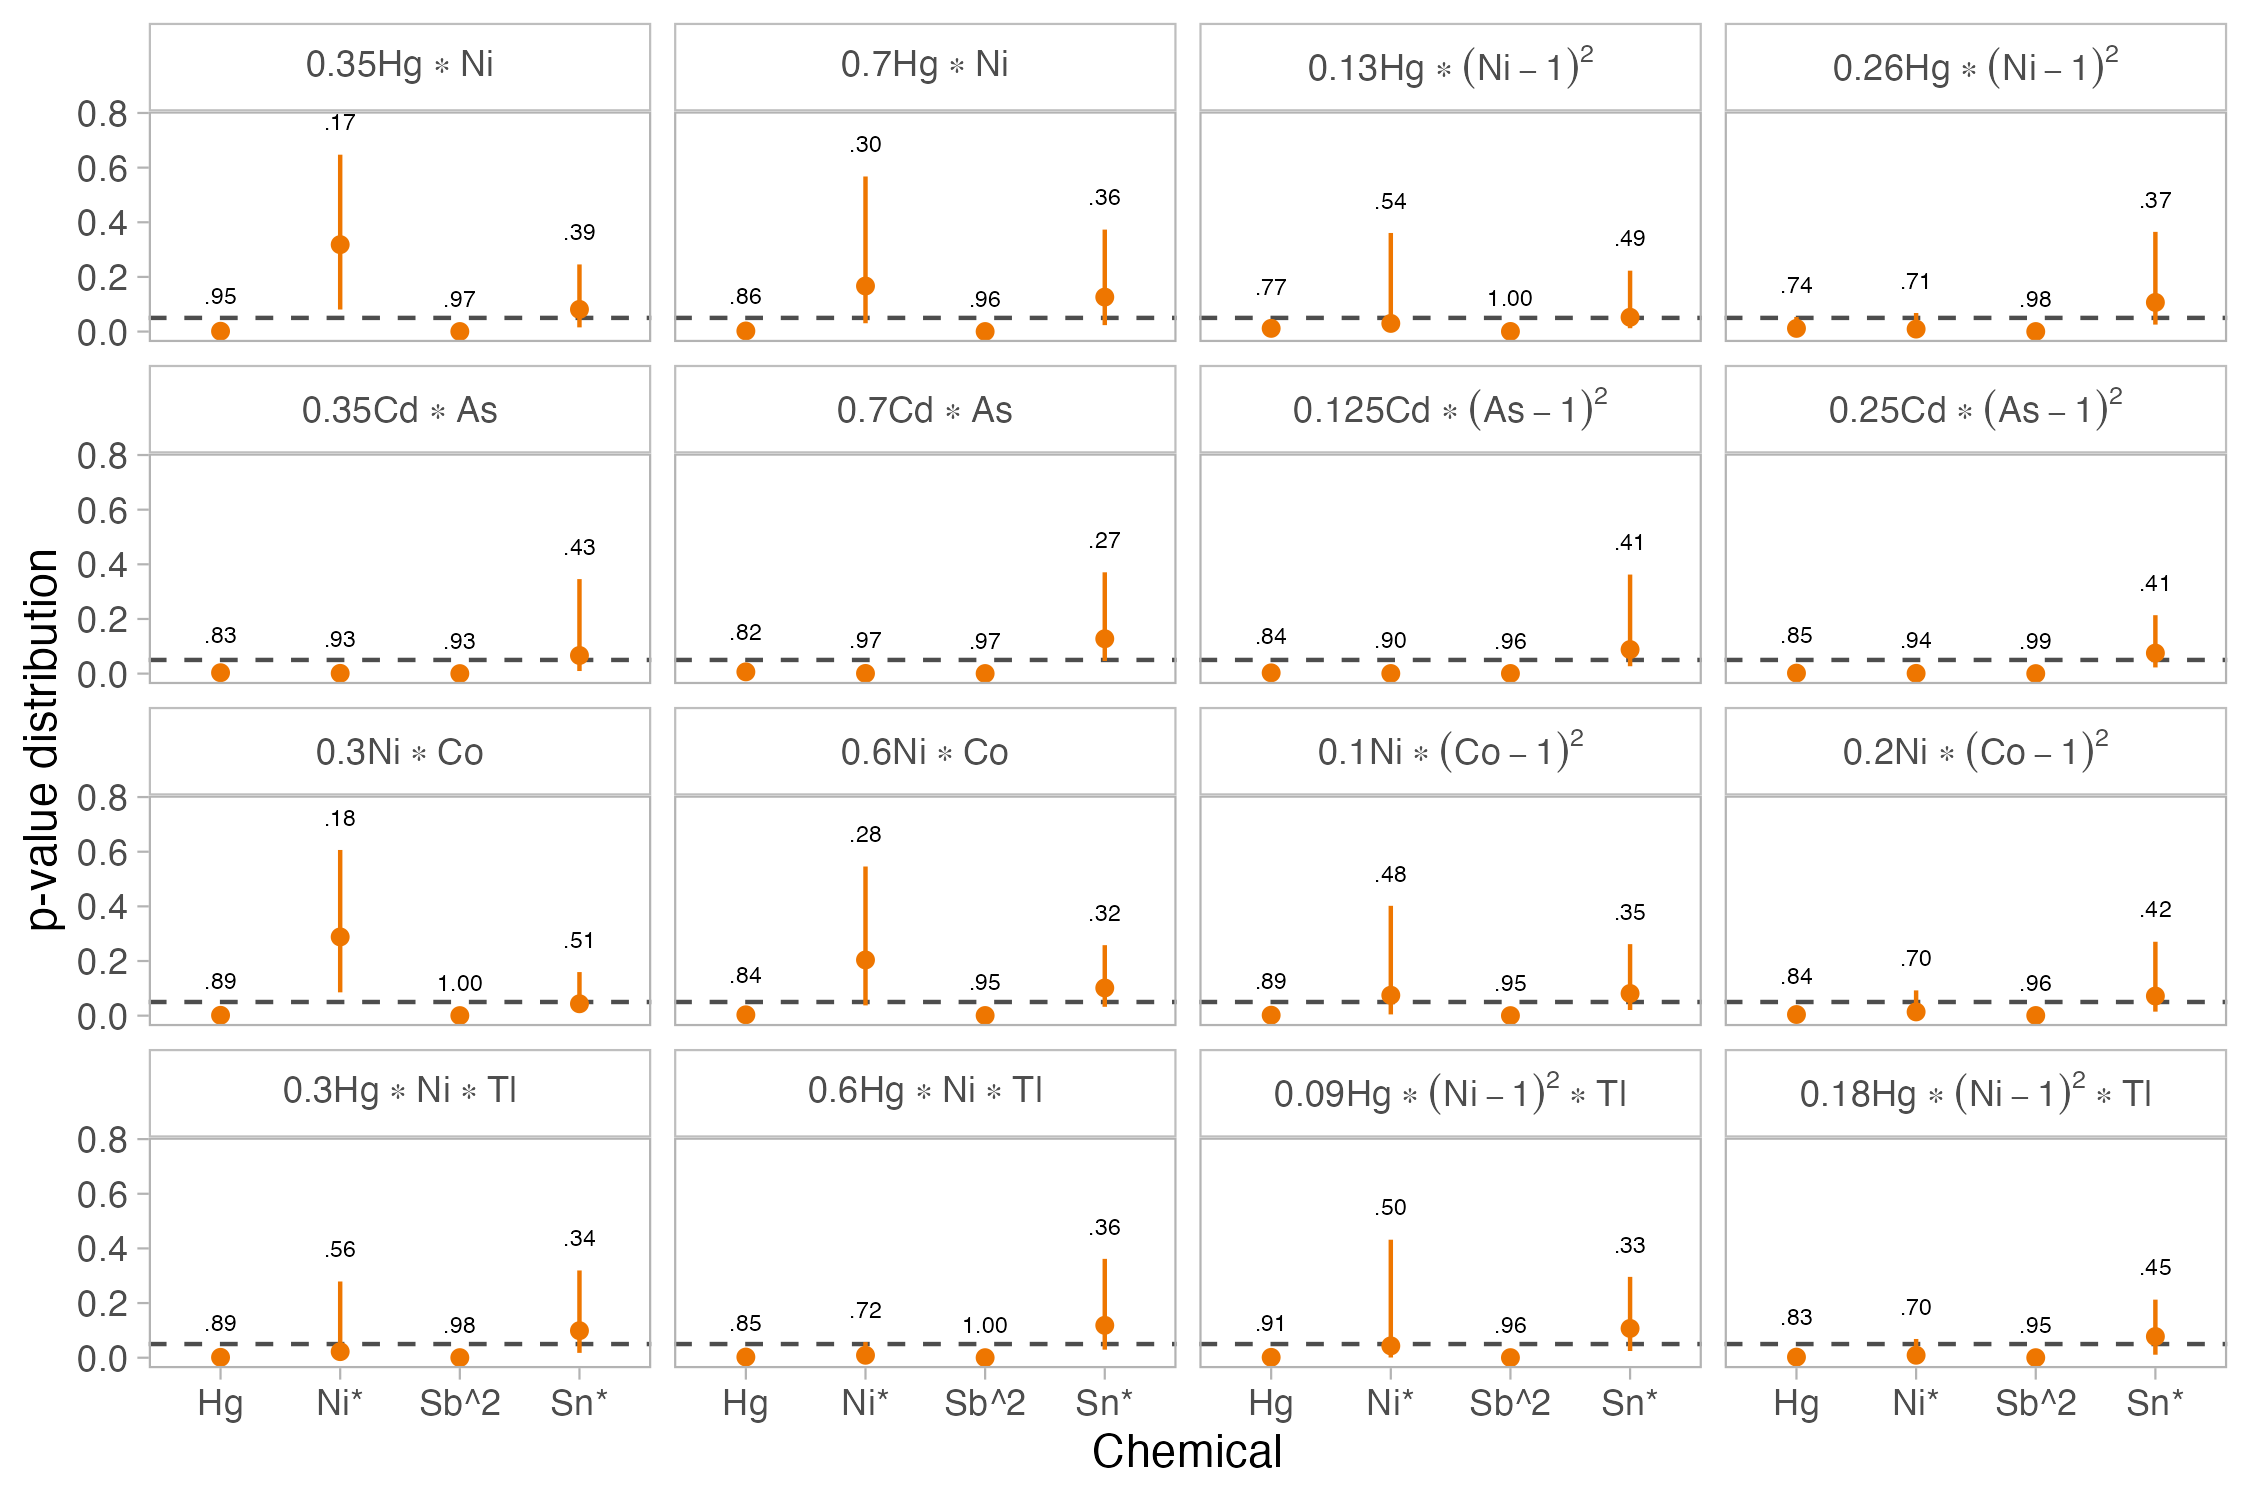
\includegraphics[width=0.8\linewidth]{figures/ch4_osm_univ_pval} 

}

\caption{P-value distributions of univariate chemicals from oracle MLRs run on smaller size (n=252) datasets, in all scenarios with interactions between chemicals. Sensitivities are displayed above a point-range with the median and first and third quartiles.}\label{fig:osmunivp}
\end{figure}
\begin{figure}

{\centering 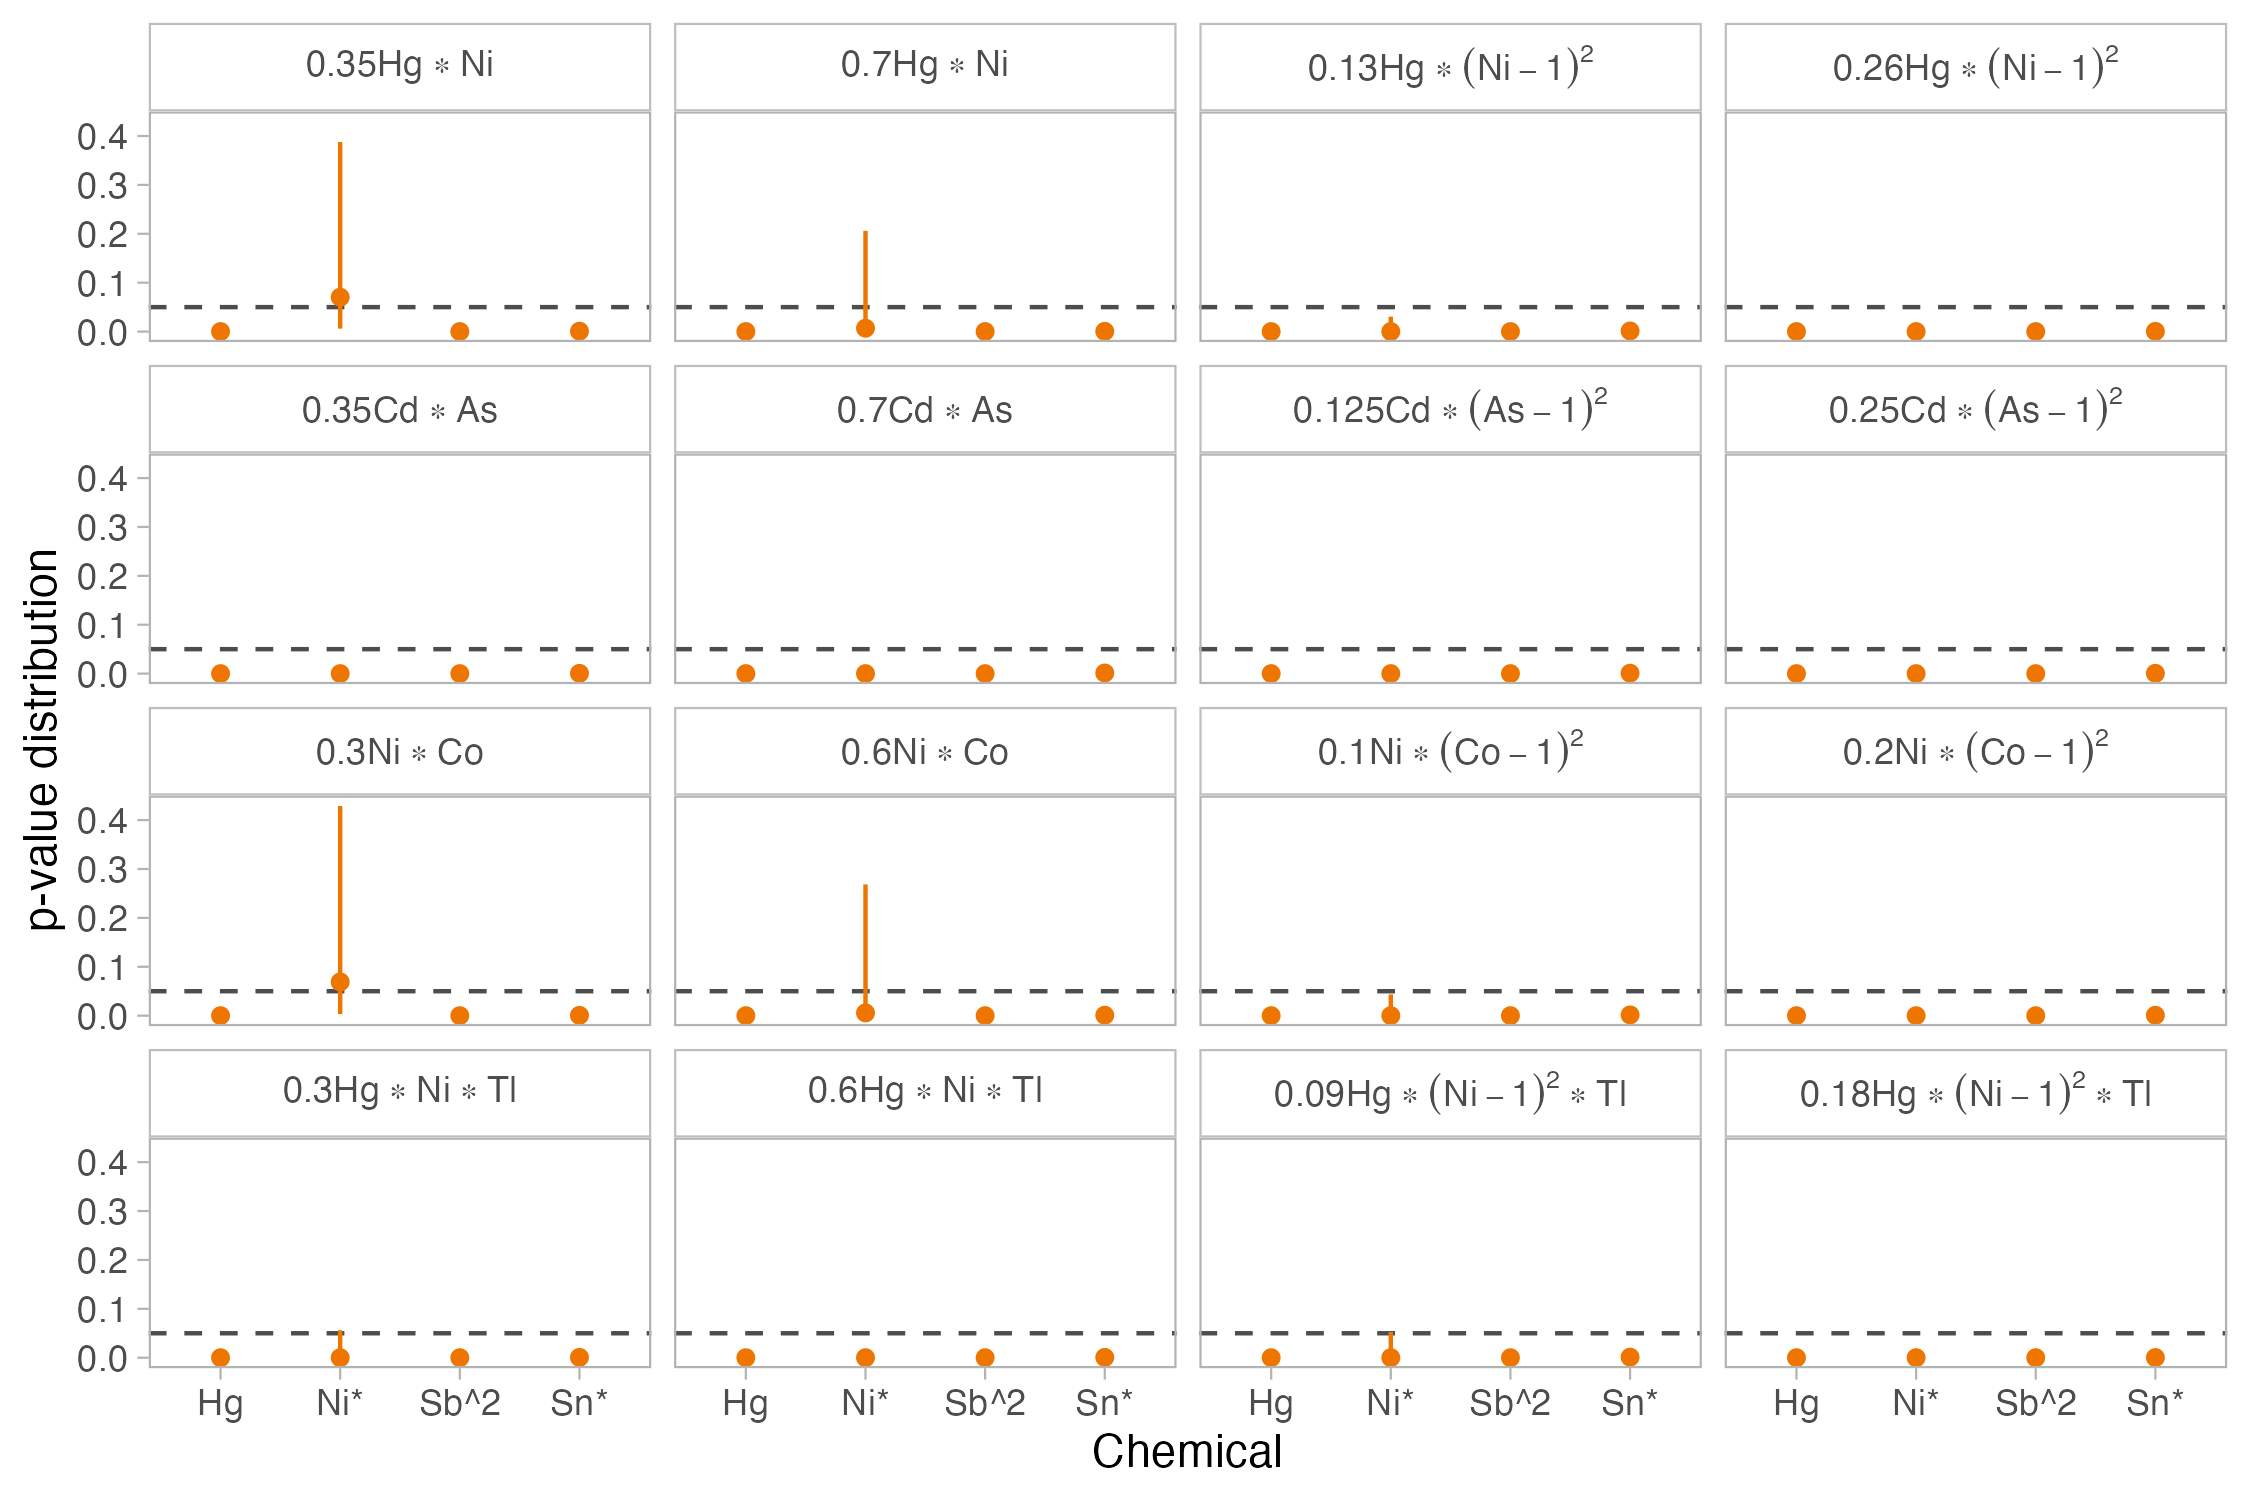
\includegraphics[width=0.8\linewidth]{figures/ch4_olg_univ_pval} 

}

\caption{P-value distributions of univariate chemicals from oracle MLRs run on larger size (n=1000) datasets, in all scenarios with interactions between chemicals. Sensitivities are displayed above a point-range with the median and first and third quartiles.}\label{fig:olgunivp}
\end{figure}
\begin{figure}

{\centering 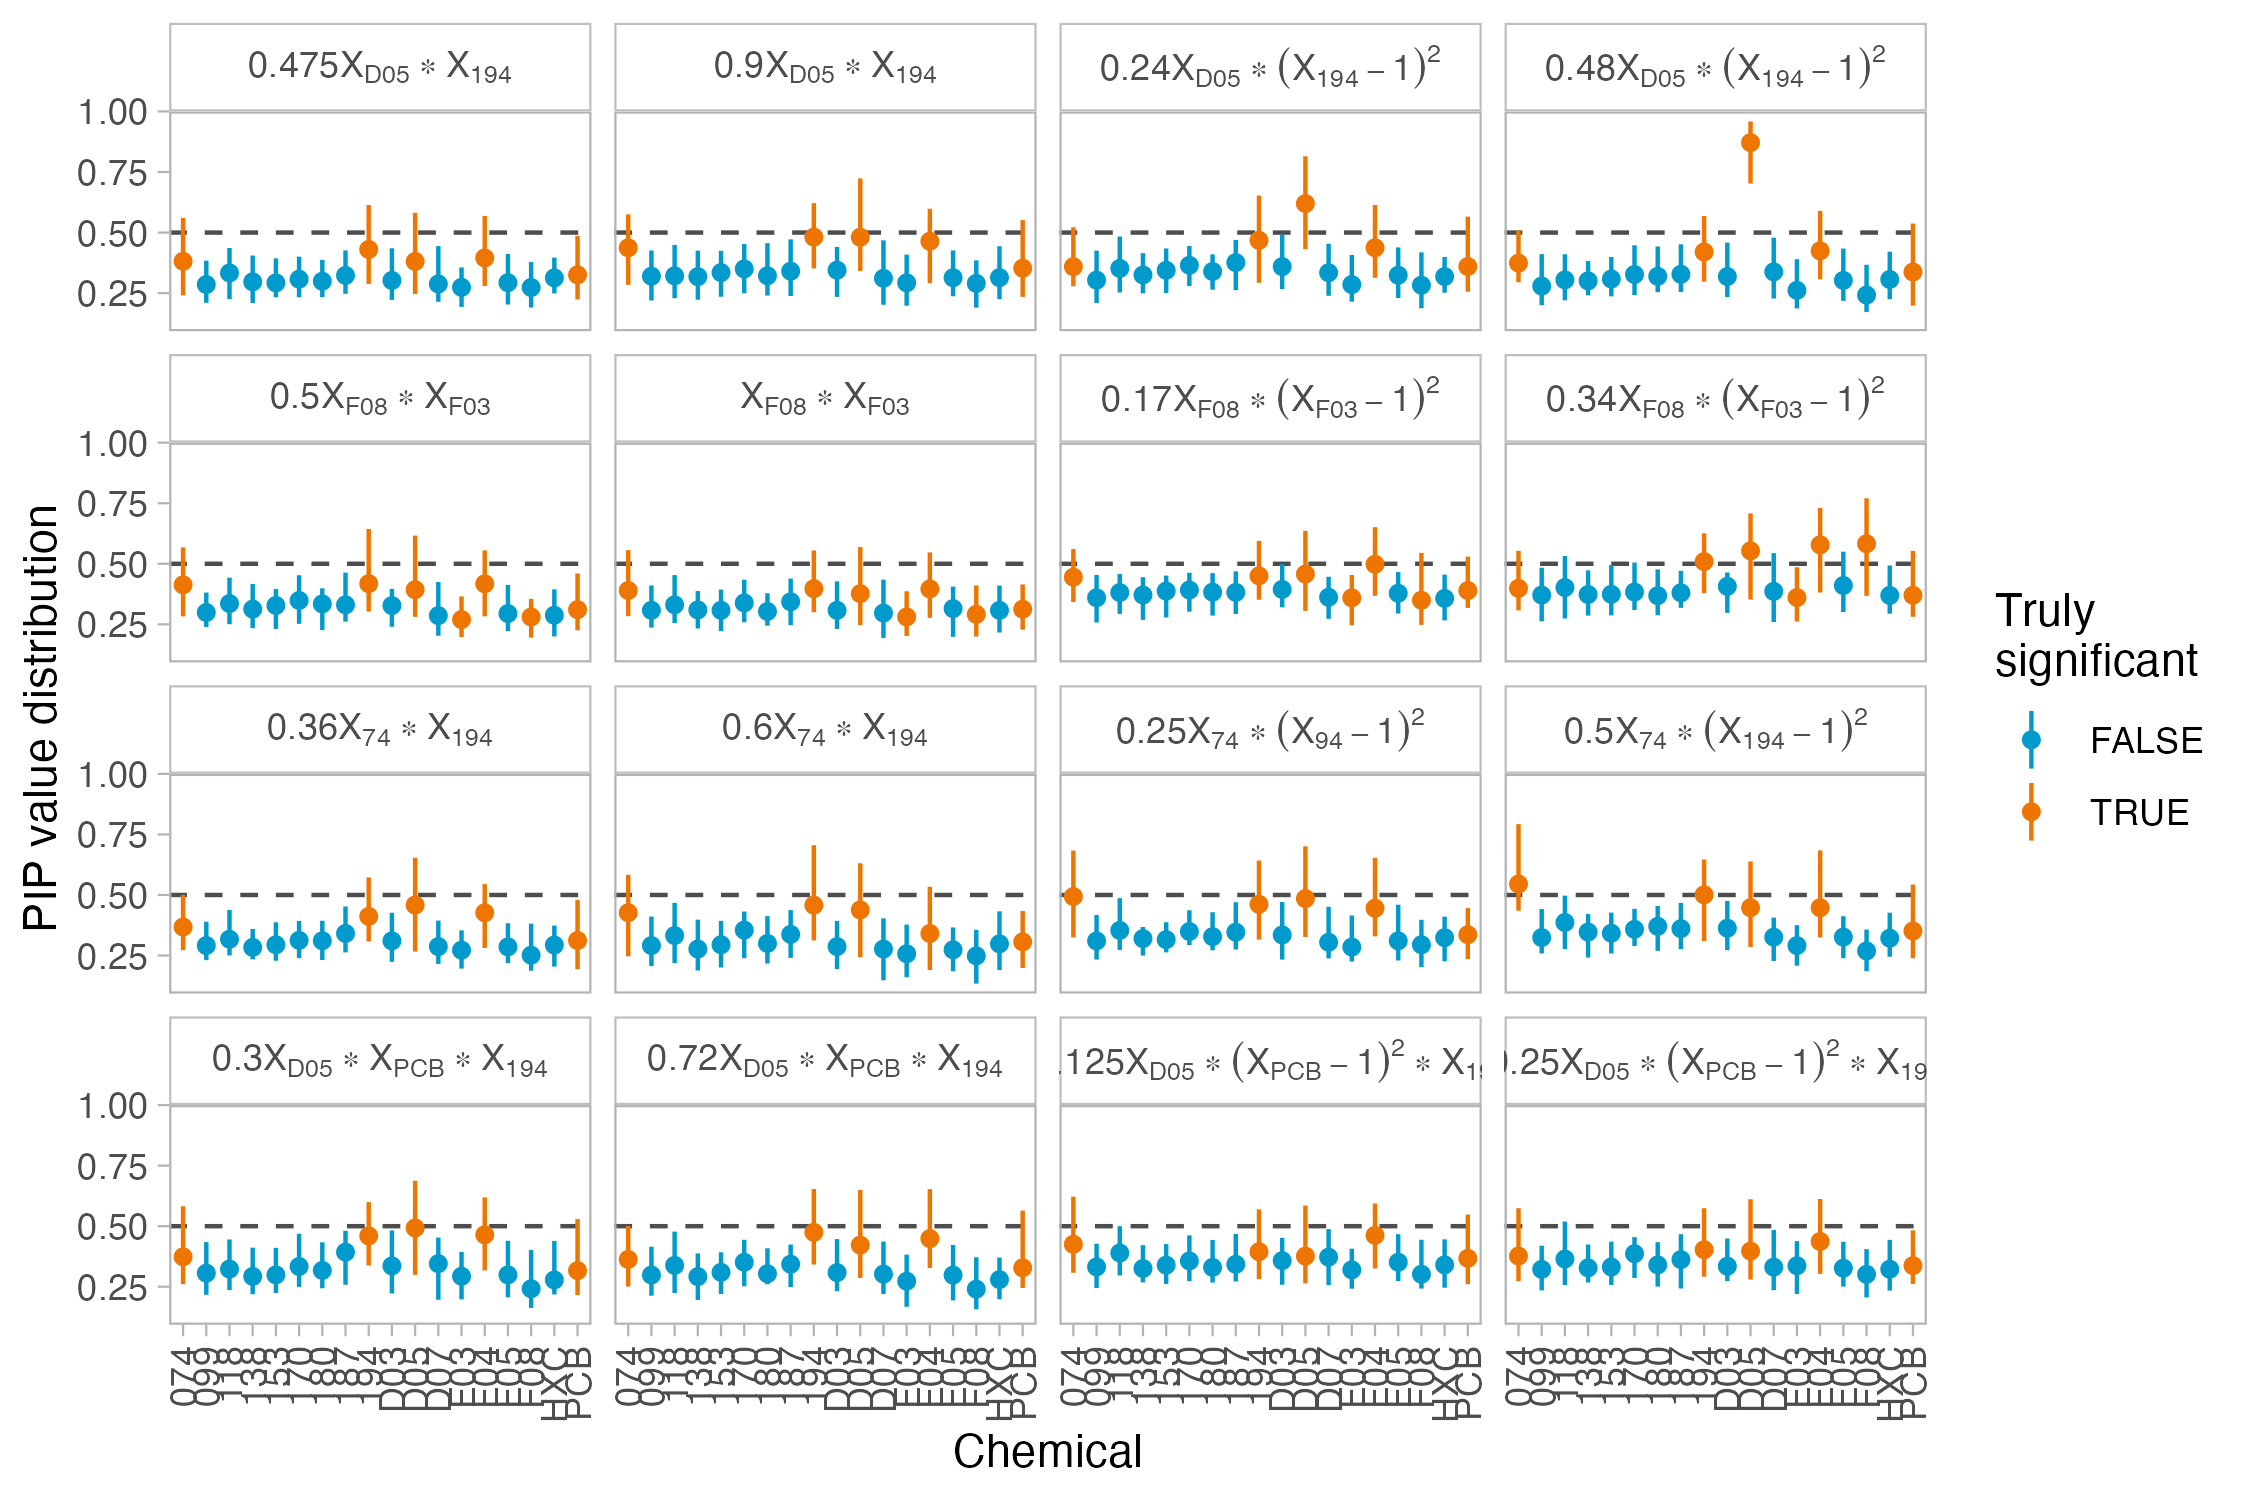
\includegraphics[width=0.8\linewidth]{figures/ch4_ksm_univ_pips} 

}

\caption{PIP distributions of univariate chemicals from BKMR models run on smaller size (n=252) datasets, in all scenarios with interactions between chemicals. Detection rates are displayed above a point-range with the median and first and third quartiles.}\label{fig:ksmunivp}
\end{figure}
\begin{figure}

{\centering 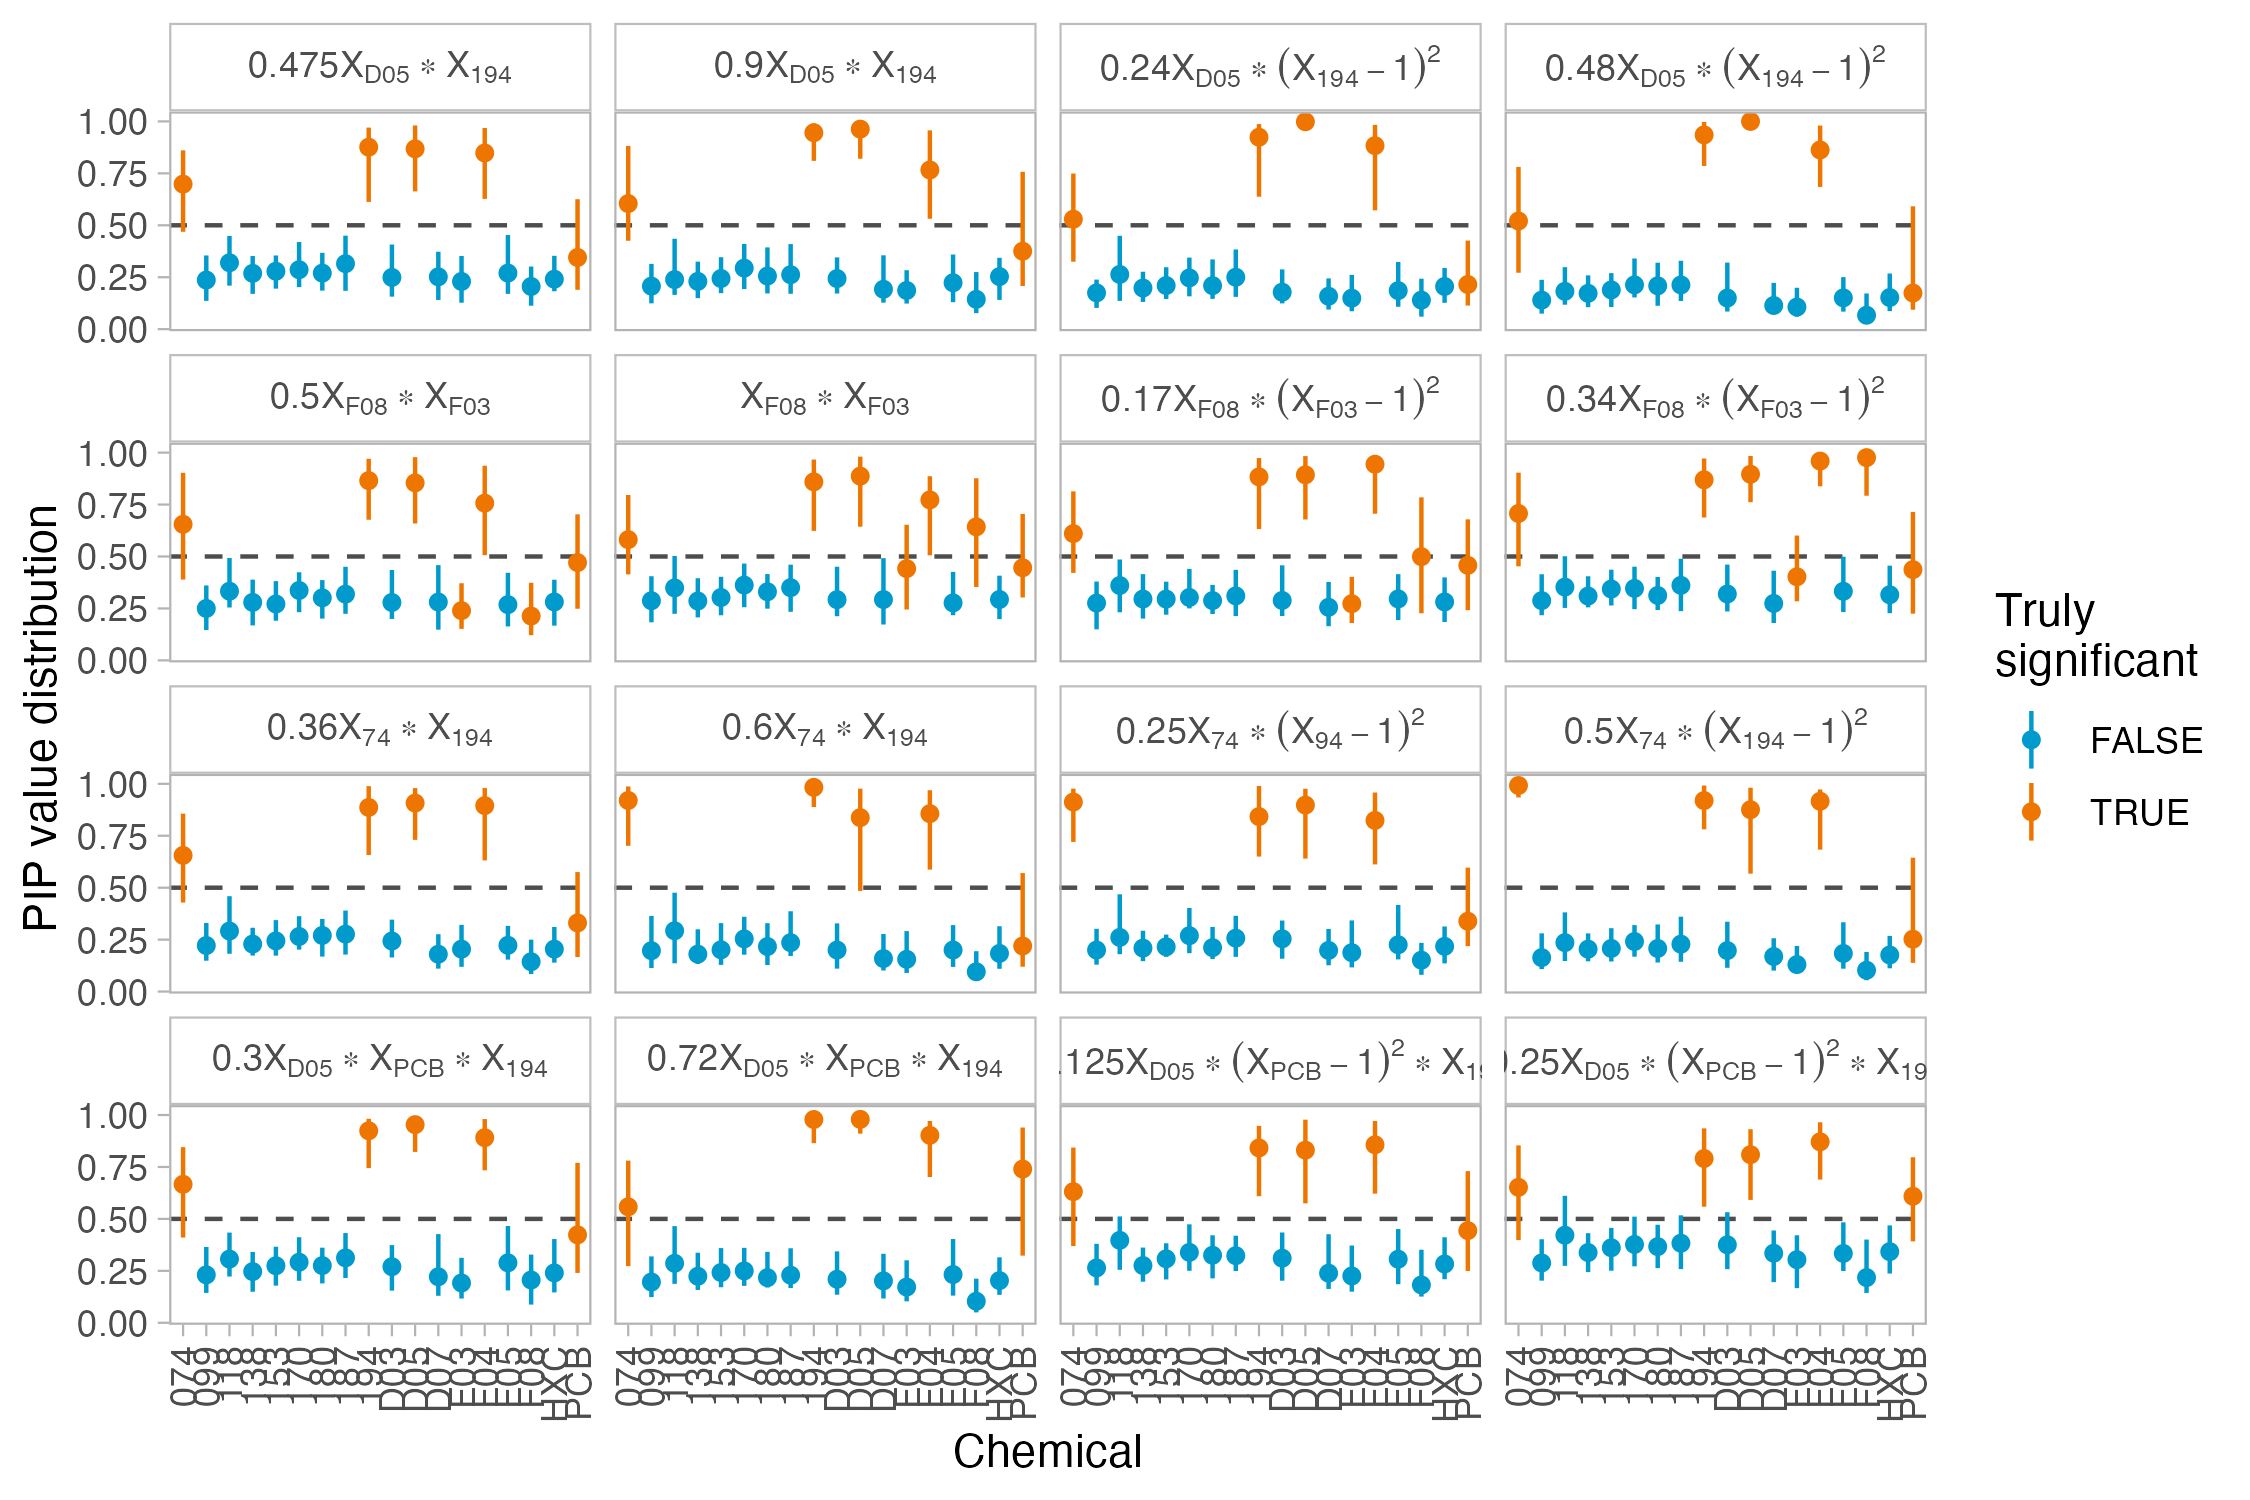
\includegraphics[width=0.8\linewidth]{figures/ch4_klg_univ_pips} 

}

\caption{PIP distributions of univariate chemicals from BKMR models run on larger size (n=1000) datasets, in all scenarios with interactions between chemicals. Detection rates are displayed above a point-range with the median and first and third quartiles.}\label{fig:klgunivp}
\end{figure}
\begin{figure}

{\centering 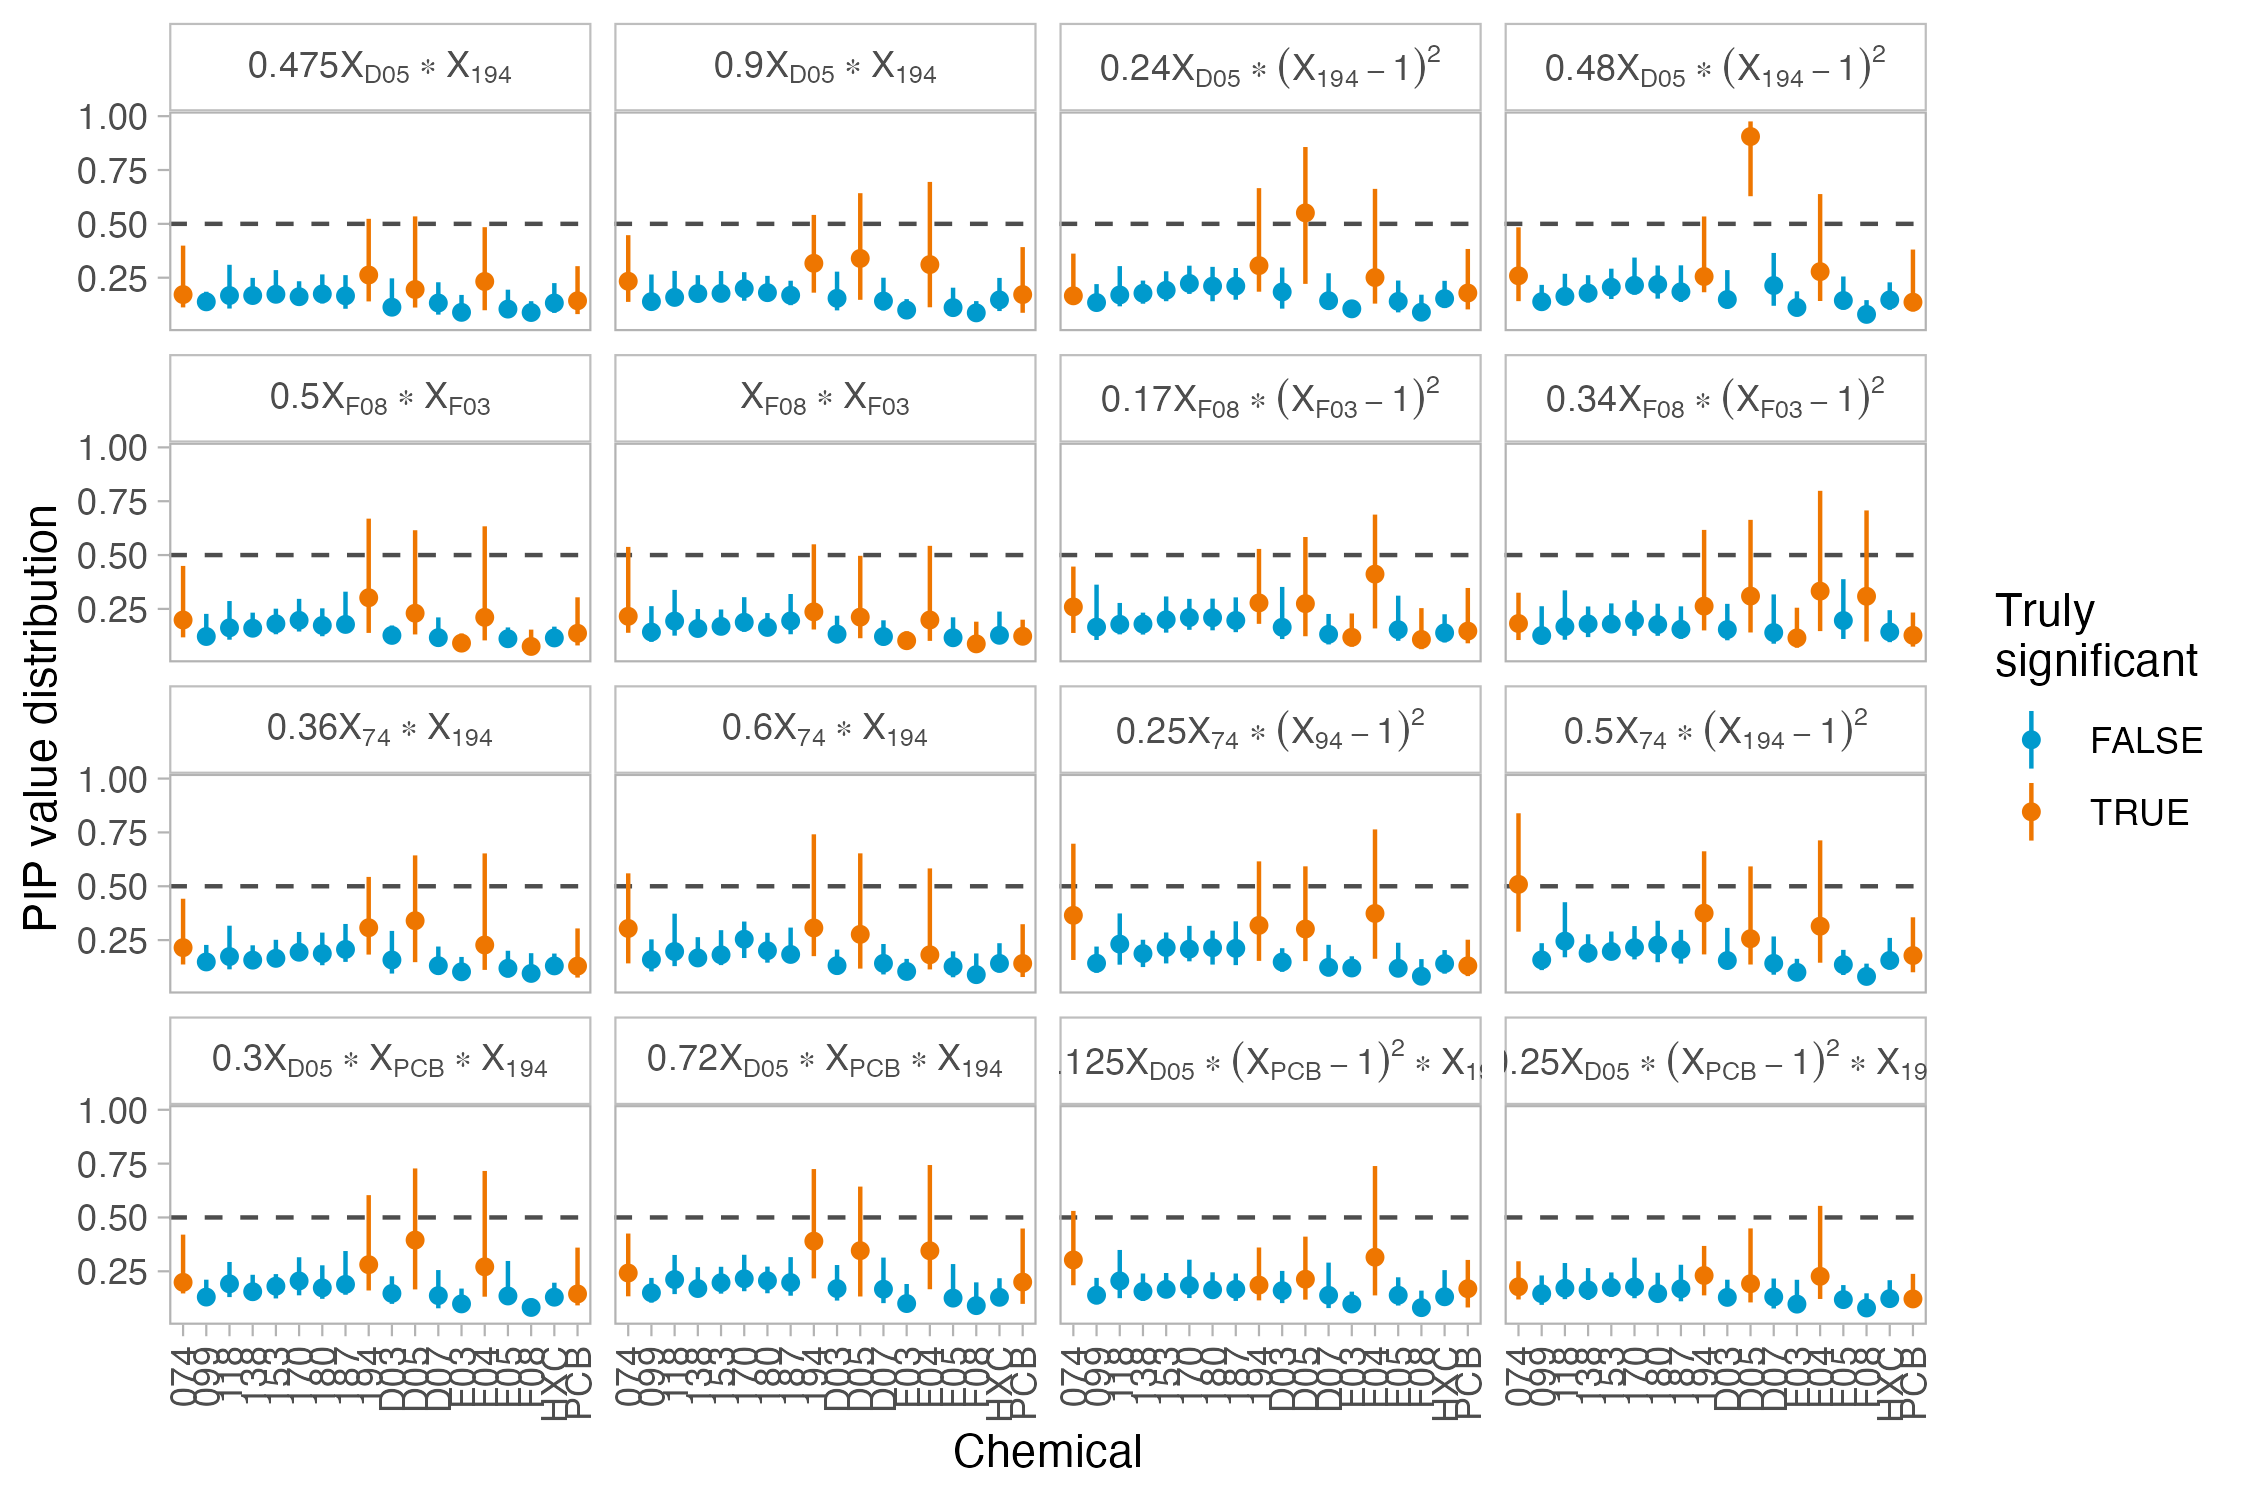
\includegraphics[width=0.8\linewidth]{figures/ch4_ssm_univ_pips} 

}

\caption{PIP distributions of univariate chemicals from BSR models run on smaller size (n=252) datasets, in all scenarios with interactions between chemicals. Detection rates are displayed above a point-range with the median and first and third quartiles.}\label{fig:ssmunivp}
\end{figure}
\begin{figure}

{\centering 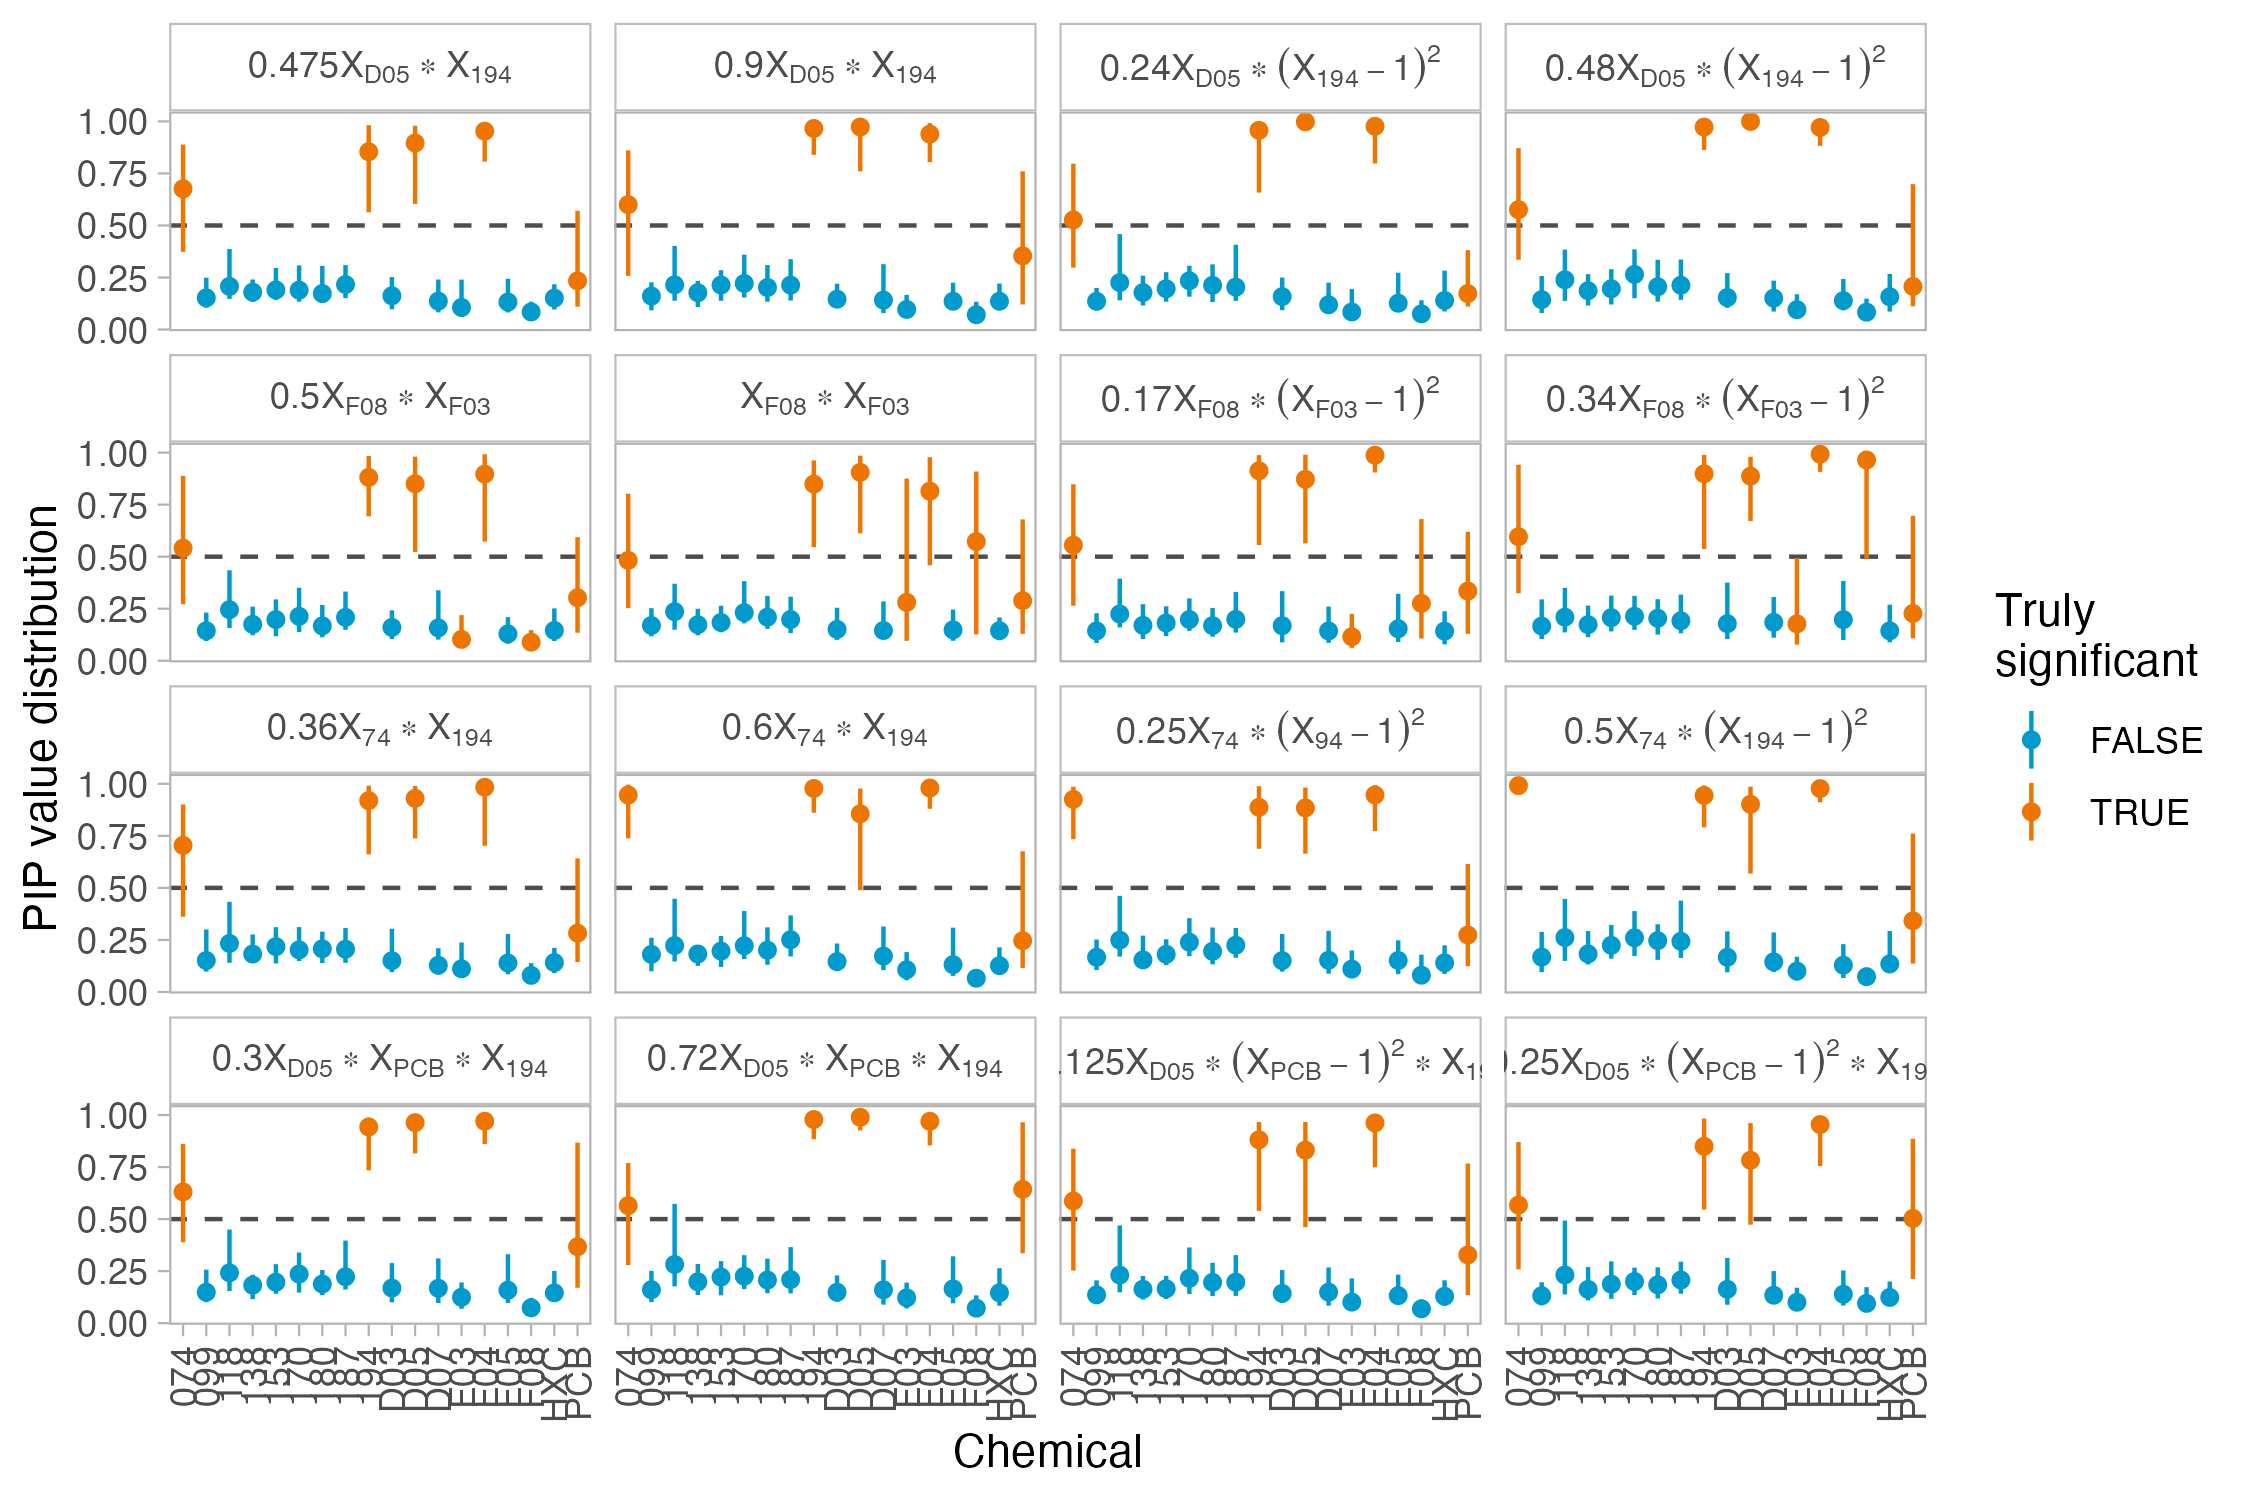
\includegraphics[width=0.8\linewidth]{figures/ch4_slg_univ_pips} 

}

\caption{PIP distributions of univariate chemicals from BSR models run on larger size (n=252) datasets, in all scenarios with interactions between chemicals. Detection rates are displayed above a point-range with the median and first and third quartiles.}\label{fig:slgunivp}
\end{figure}
Figures \ref{fig:osmbivp} and \ref{fig:olgbivp} display the full p-value distributions on interaction terms between chemicals in the oracle MLR models.
\begin{figure}

{\centering 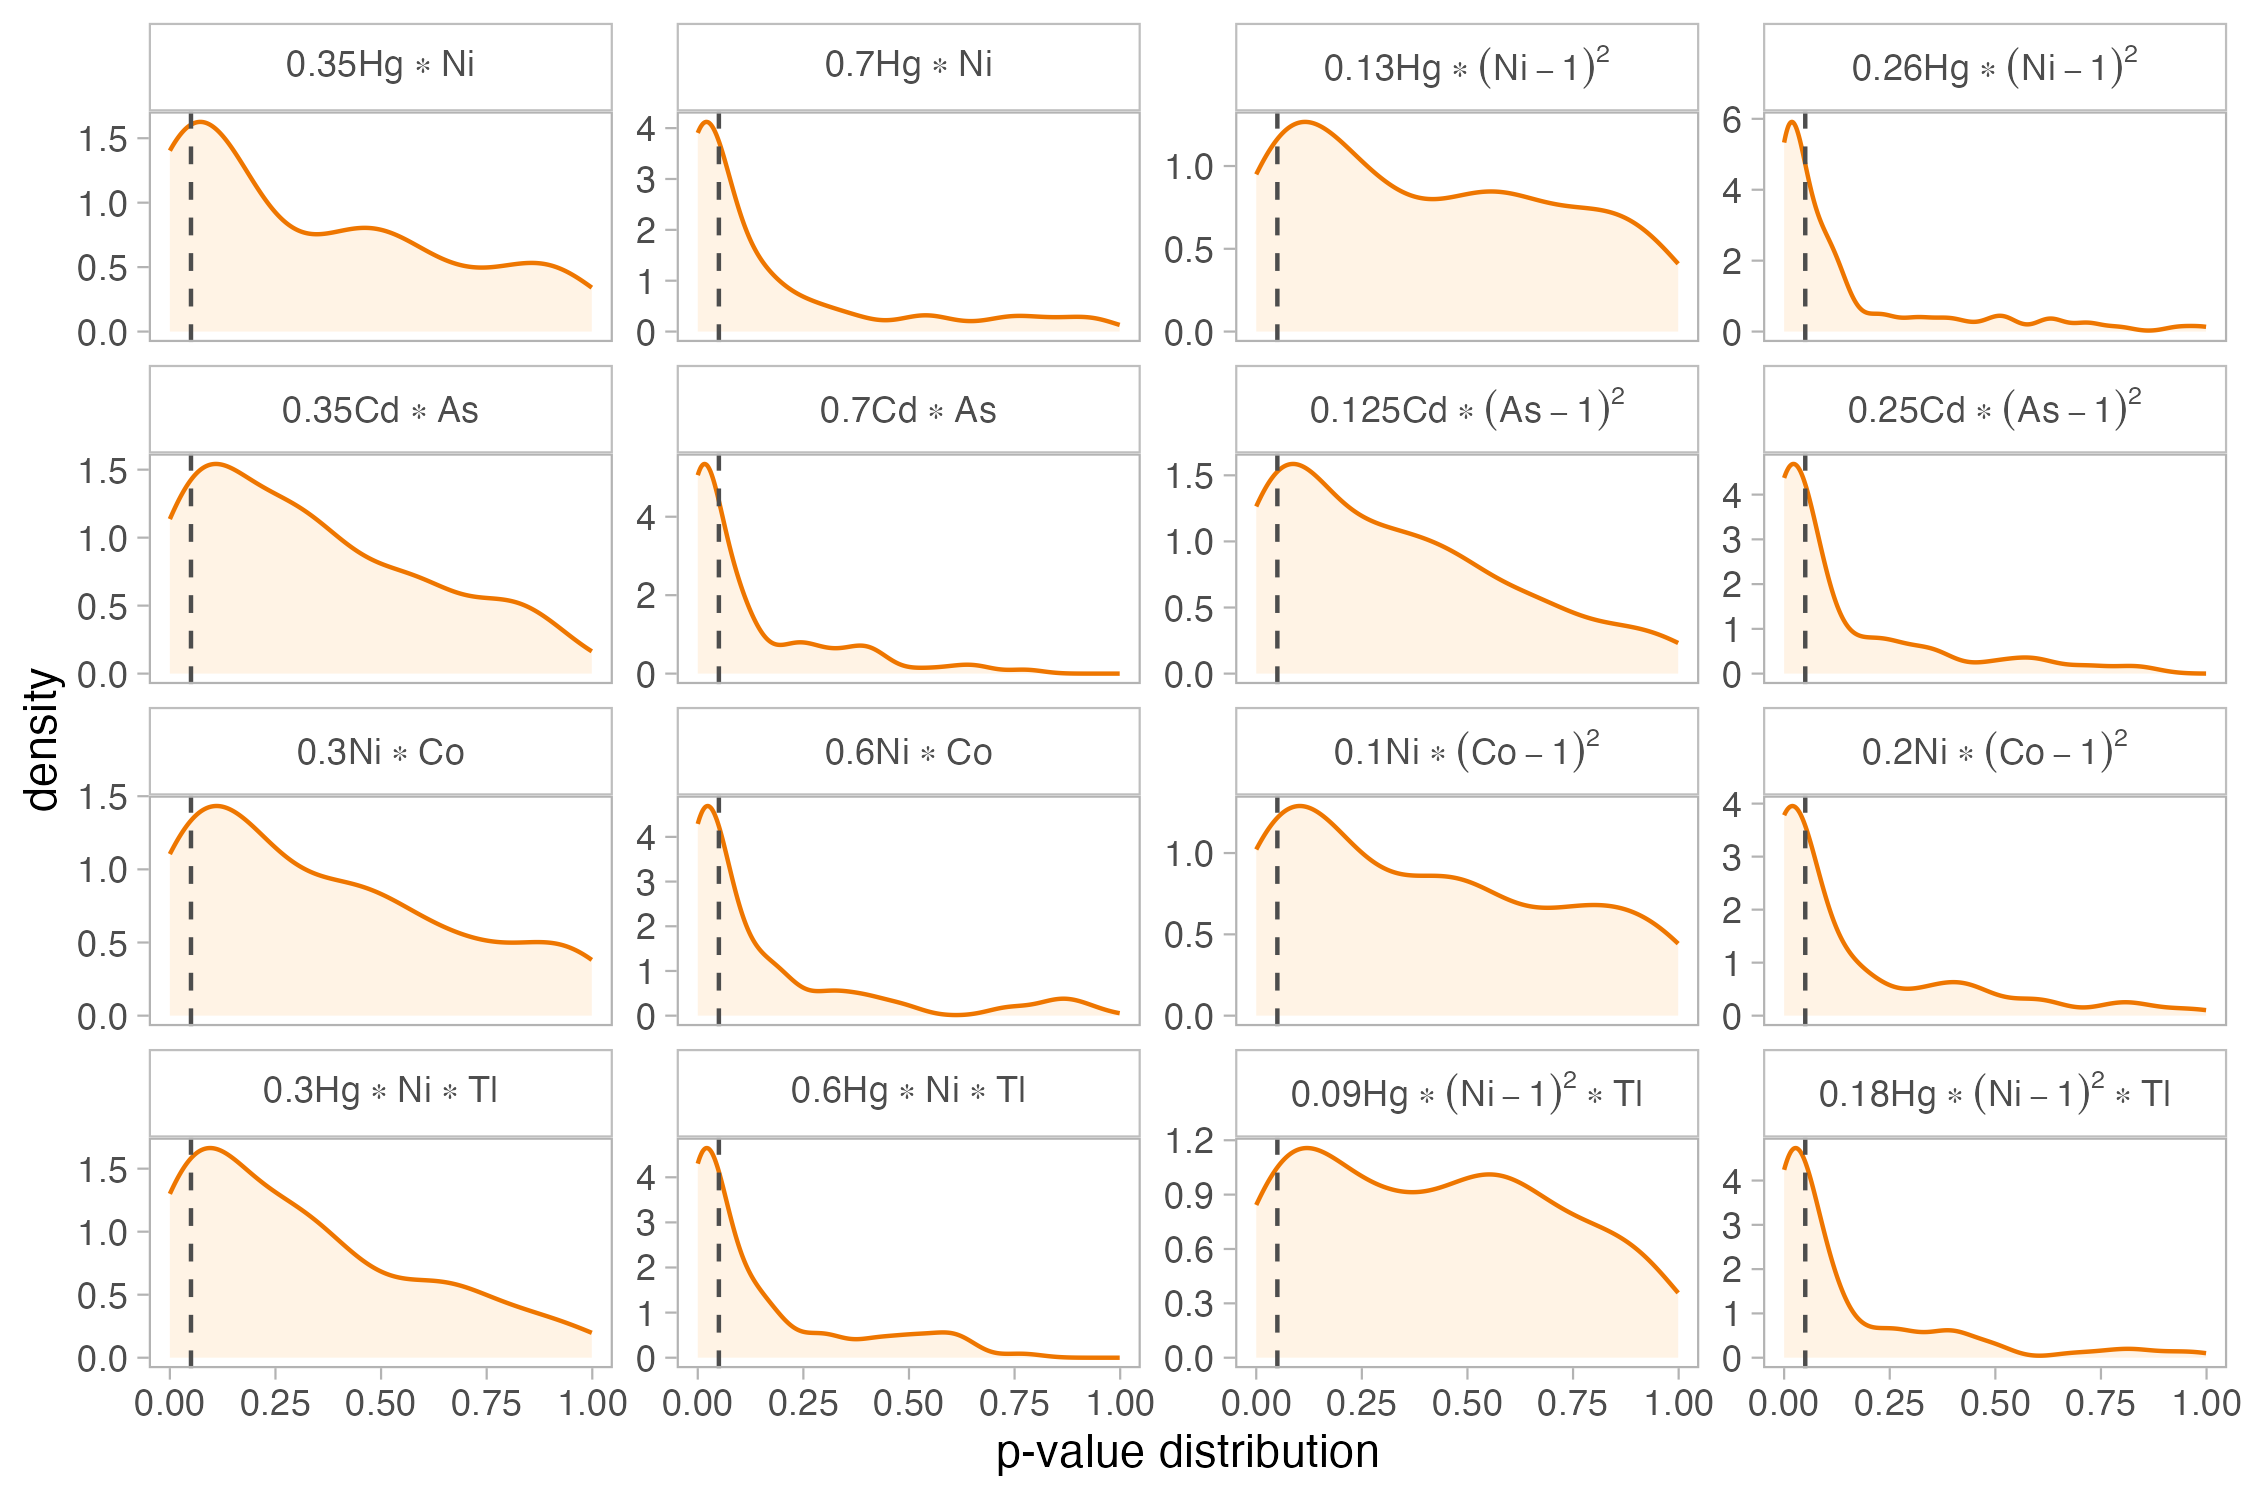
\includegraphics[width=0.8\linewidth]{figures/ch4_osm_biv_pval} 

}

\caption{P-value distributions of interaction terms from oracle MLRs run on smaller size (n=252) datasets, from all scenarios with interactions between chemicals.}\label{fig:osmbivp}
\end{figure}
\begin{figure}

{\centering 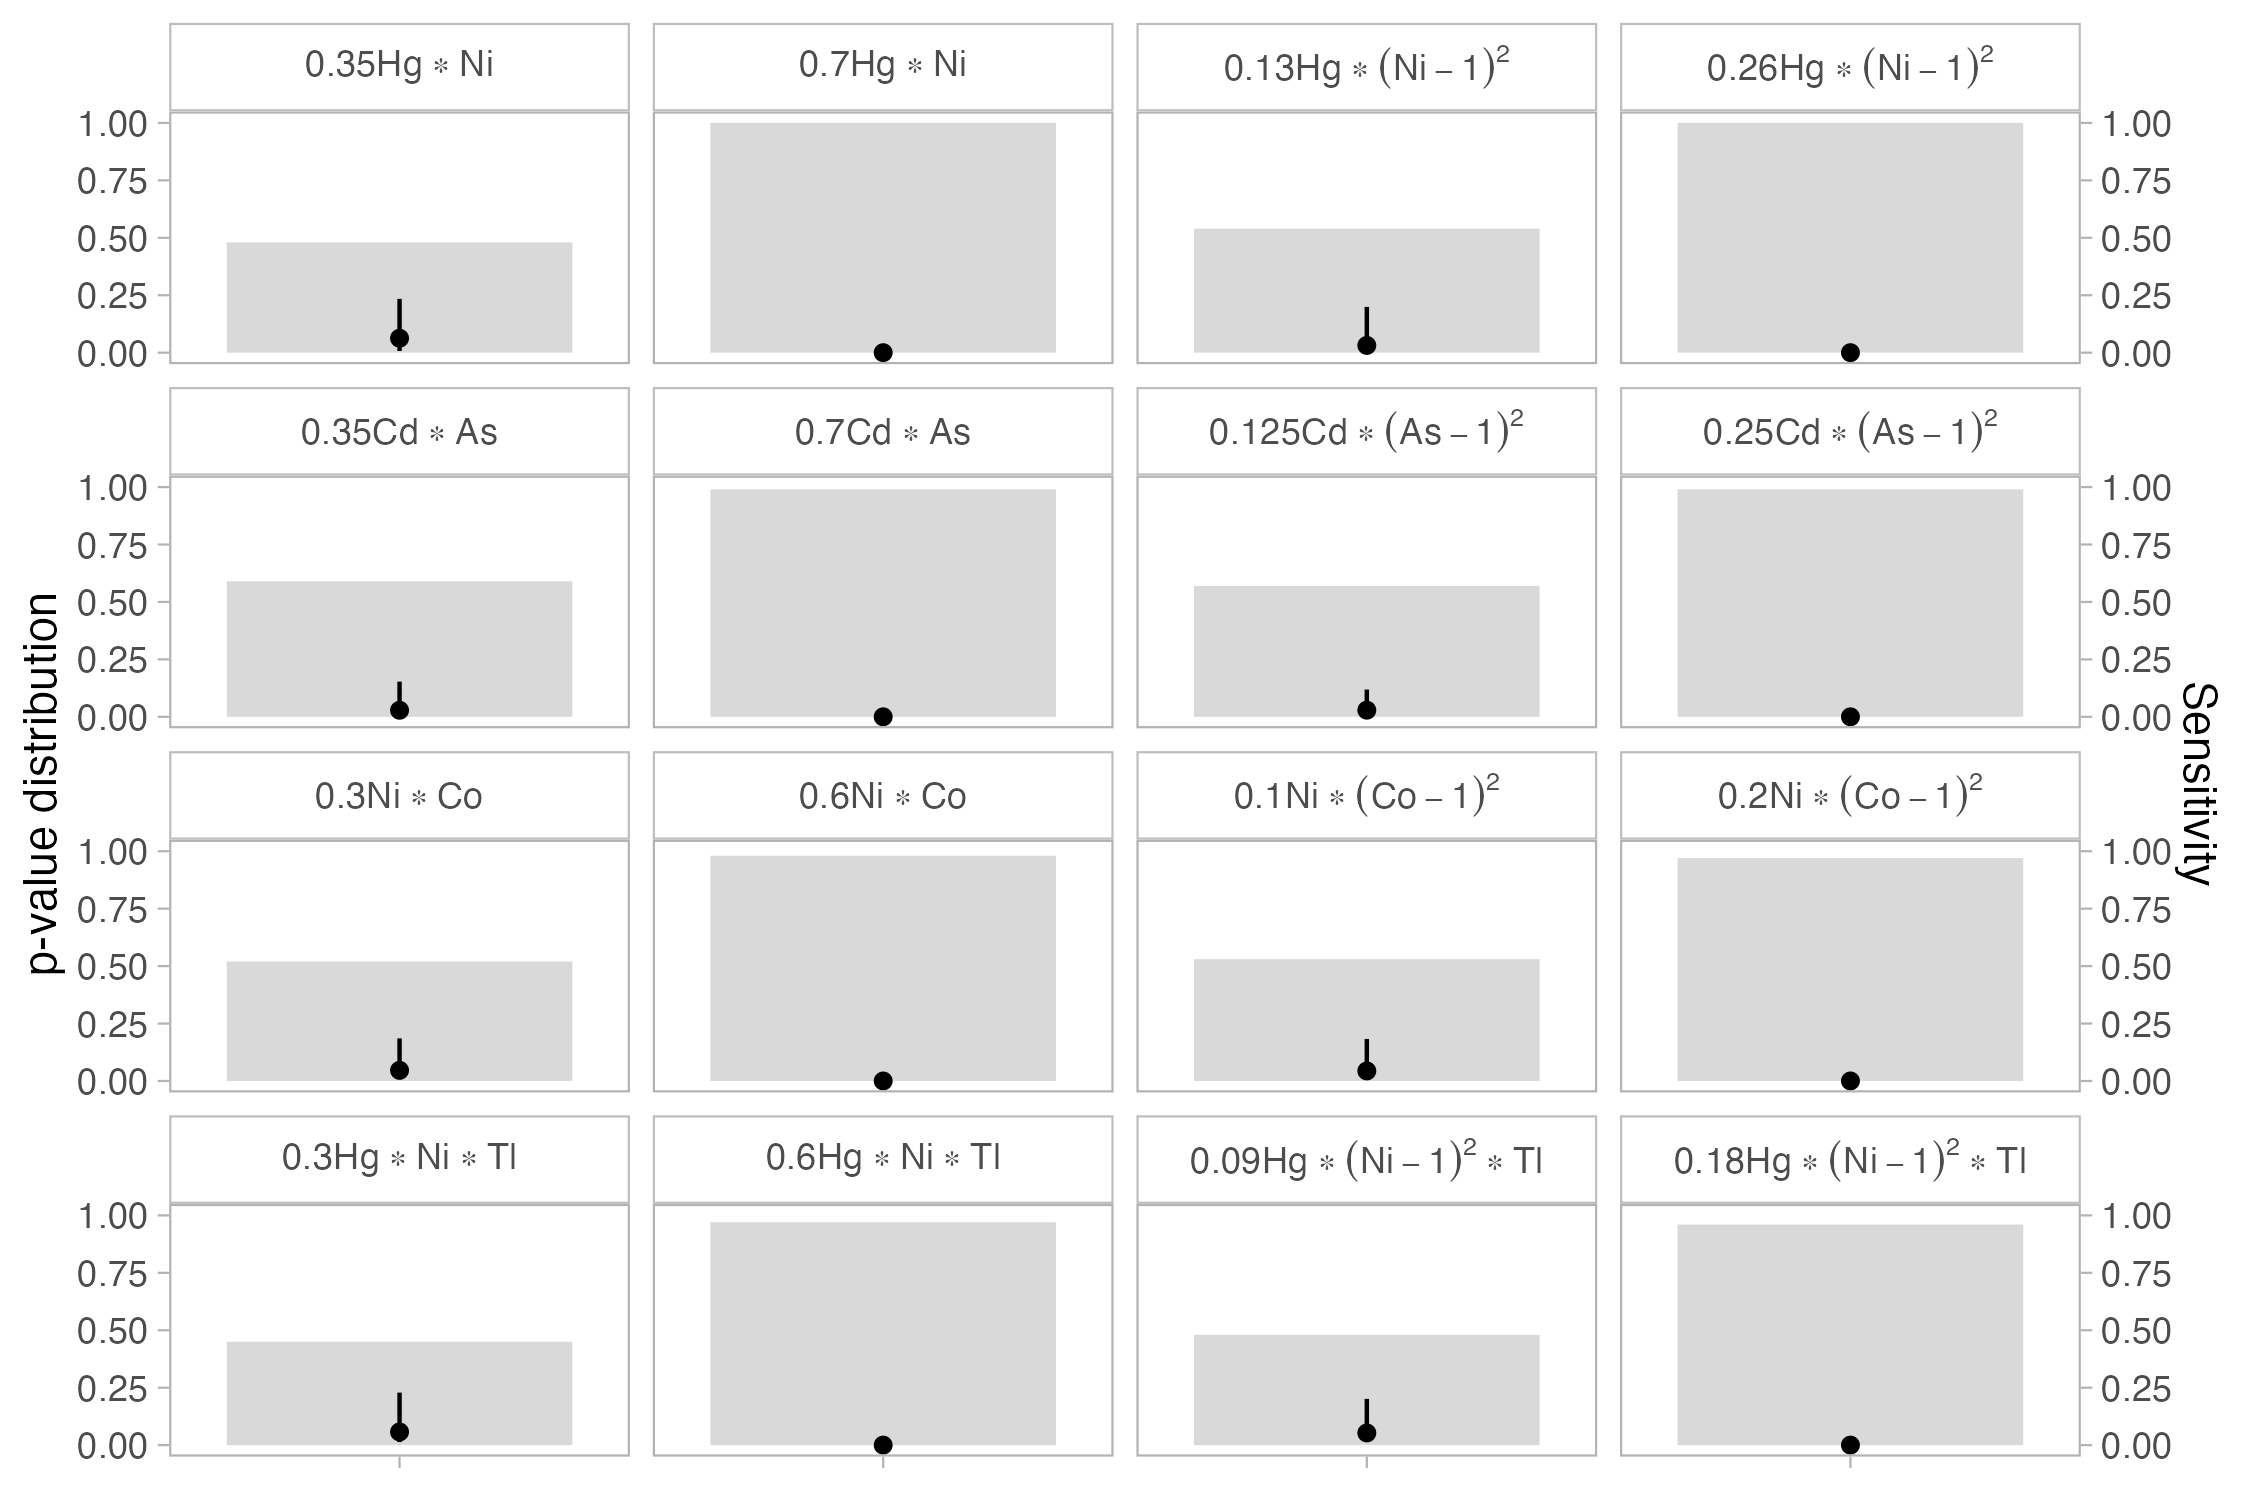
\includegraphics[width=0.8\linewidth]{figures/ch4_olg_biv_pval} 

}

\caption{P-value distributions of interaction terms from oracle MLRs run on larger size (n=1000) datasets, from all scenarios with interactions between chemicals.}\label{fig:olgbivp}
\end{figure}
Table \ref{tab:onewaytabfdr} summarizes the sensitivities and false discovery rates for univariate terms in scenarios with interactions between chemicals.
\begin{table}

\caption{\label{tab:onewaytabfdr}Overall false discovery rate for univariate chemicals in all scenarios with interactions between chemicals.}
\centering
\begin{tabular}[t]{llrrrrrr}
\toprule
\multicolumn{2}{c}{ } & \multicolumn{3}{c}{Small} & \multicolumn{3}{c}{Large} \\
\cmidrule(l{3pt}r{3pt}){3-5} \cmidrule(l{3pt}r{3pt}){6-8}
Type & Effect size & Naive & BKMR & BSR & Naive & BKMR & BSR\\
\midrule
\addlinespace[0.3em]
\multicolumn{8}{l}{\textbf{Hg-Ni}}\\
\hspace{1em}Mult. & Lower & 0.06 & 0.34 & 0.03 & 0.07 & 0.09 & 0.03\\
\hspace{1em}Mult. & Higher & 0.03 & 0.20 & 0.04 & 0.04 & 0.04 & 0.01\\
\hspace{1em}Poly. & Lower & 0.04 & 0.29 & 0.04 & 0.04 & 0.07 & 0.00\\
\hspace{1em}Poly. & Higher & 0.05 & 0.30 & 0.05 & 0.07 & 0.09 & 0.02\\
\addlinespace[0.3em]
\multicolumn{8}{l}{\textbf{Cd-As}}\\
\hspace{1em}Mult. & Lower & 0.05 & 0.27 & 0.03 & 0.05 & 0.10 & 0.01\\
\hspace{1em}Mult. & Higher & 0.07 & 0.44 & 0.07 & 0.16 & 0.30 & 0.16\\
\hspace{1em}Poly. & Lower & 0.05 & 0.29 & 0.04 & 0.08 & 0.18 & 0.03\\
\hspace{1em}Poly. & Higher & 0.04 & 0.38 & 0.06 & 0.06 & 0.34 & 0.16\\
\addlinespace[0.3em]
\multicolumn{8}{l}{\textbf{Ni-Co}}\\
\hspace{1em}Mult. & Lower & 0.06 & 0.34 & 0.04 & 0.05 & 0.11 & 0.02\\
\hspace{1em}Mult. & Higher & 0.06 & 0.29 & 0.05 & 0.06 & 0.12 & 0.06\\
\hspace{1em}Poly. & Lower & 0.07 & 0.37 & 0.04 & 0.06 & 0.10 & 0.02\\
\hspace{1em}Poly. & Higher & 0.04 & 0.34 & 0.05 & 0.06 & 0.20 & 0.07\\
\addlinespace[0.3em]
\multicolumn{8}{l}{\textbf{Hg-Ni-Tl}}\\
\hspace{1em}Mult. & Lower & 0.06 & 0.36 & 0.04 & 0.05 & 0.08 & 0.02\\
\hspace{1em}Mult. & Higher & 0.04 & 0.36 & 0.04 & 0.04 & 0.16 & 0.03\\
\hspace{1em}Poly. & Lower & 0.05 & 0.35 & 0.05 & 0.06 & 0.13 & 0.02\\
\hspace{1em}Poly. & Higher & 0.06 & 0.26 & 0.03 & 0.05 & 0.08 & 0.03\\
\bottomrule
\end{tabular}
\end{table}
Figures \ref{fig:ksmcdas}-\ref{fig:slgtri} display the estimated exposure-response surface for one chemical while fixing one (or two, for three-way interactions) other chemicals at their 0.1, 0.5, and 0.9 quantiles, for all scenarios not included in Chapter \ref{univsenschap}.
\begin{figure}

{\centering 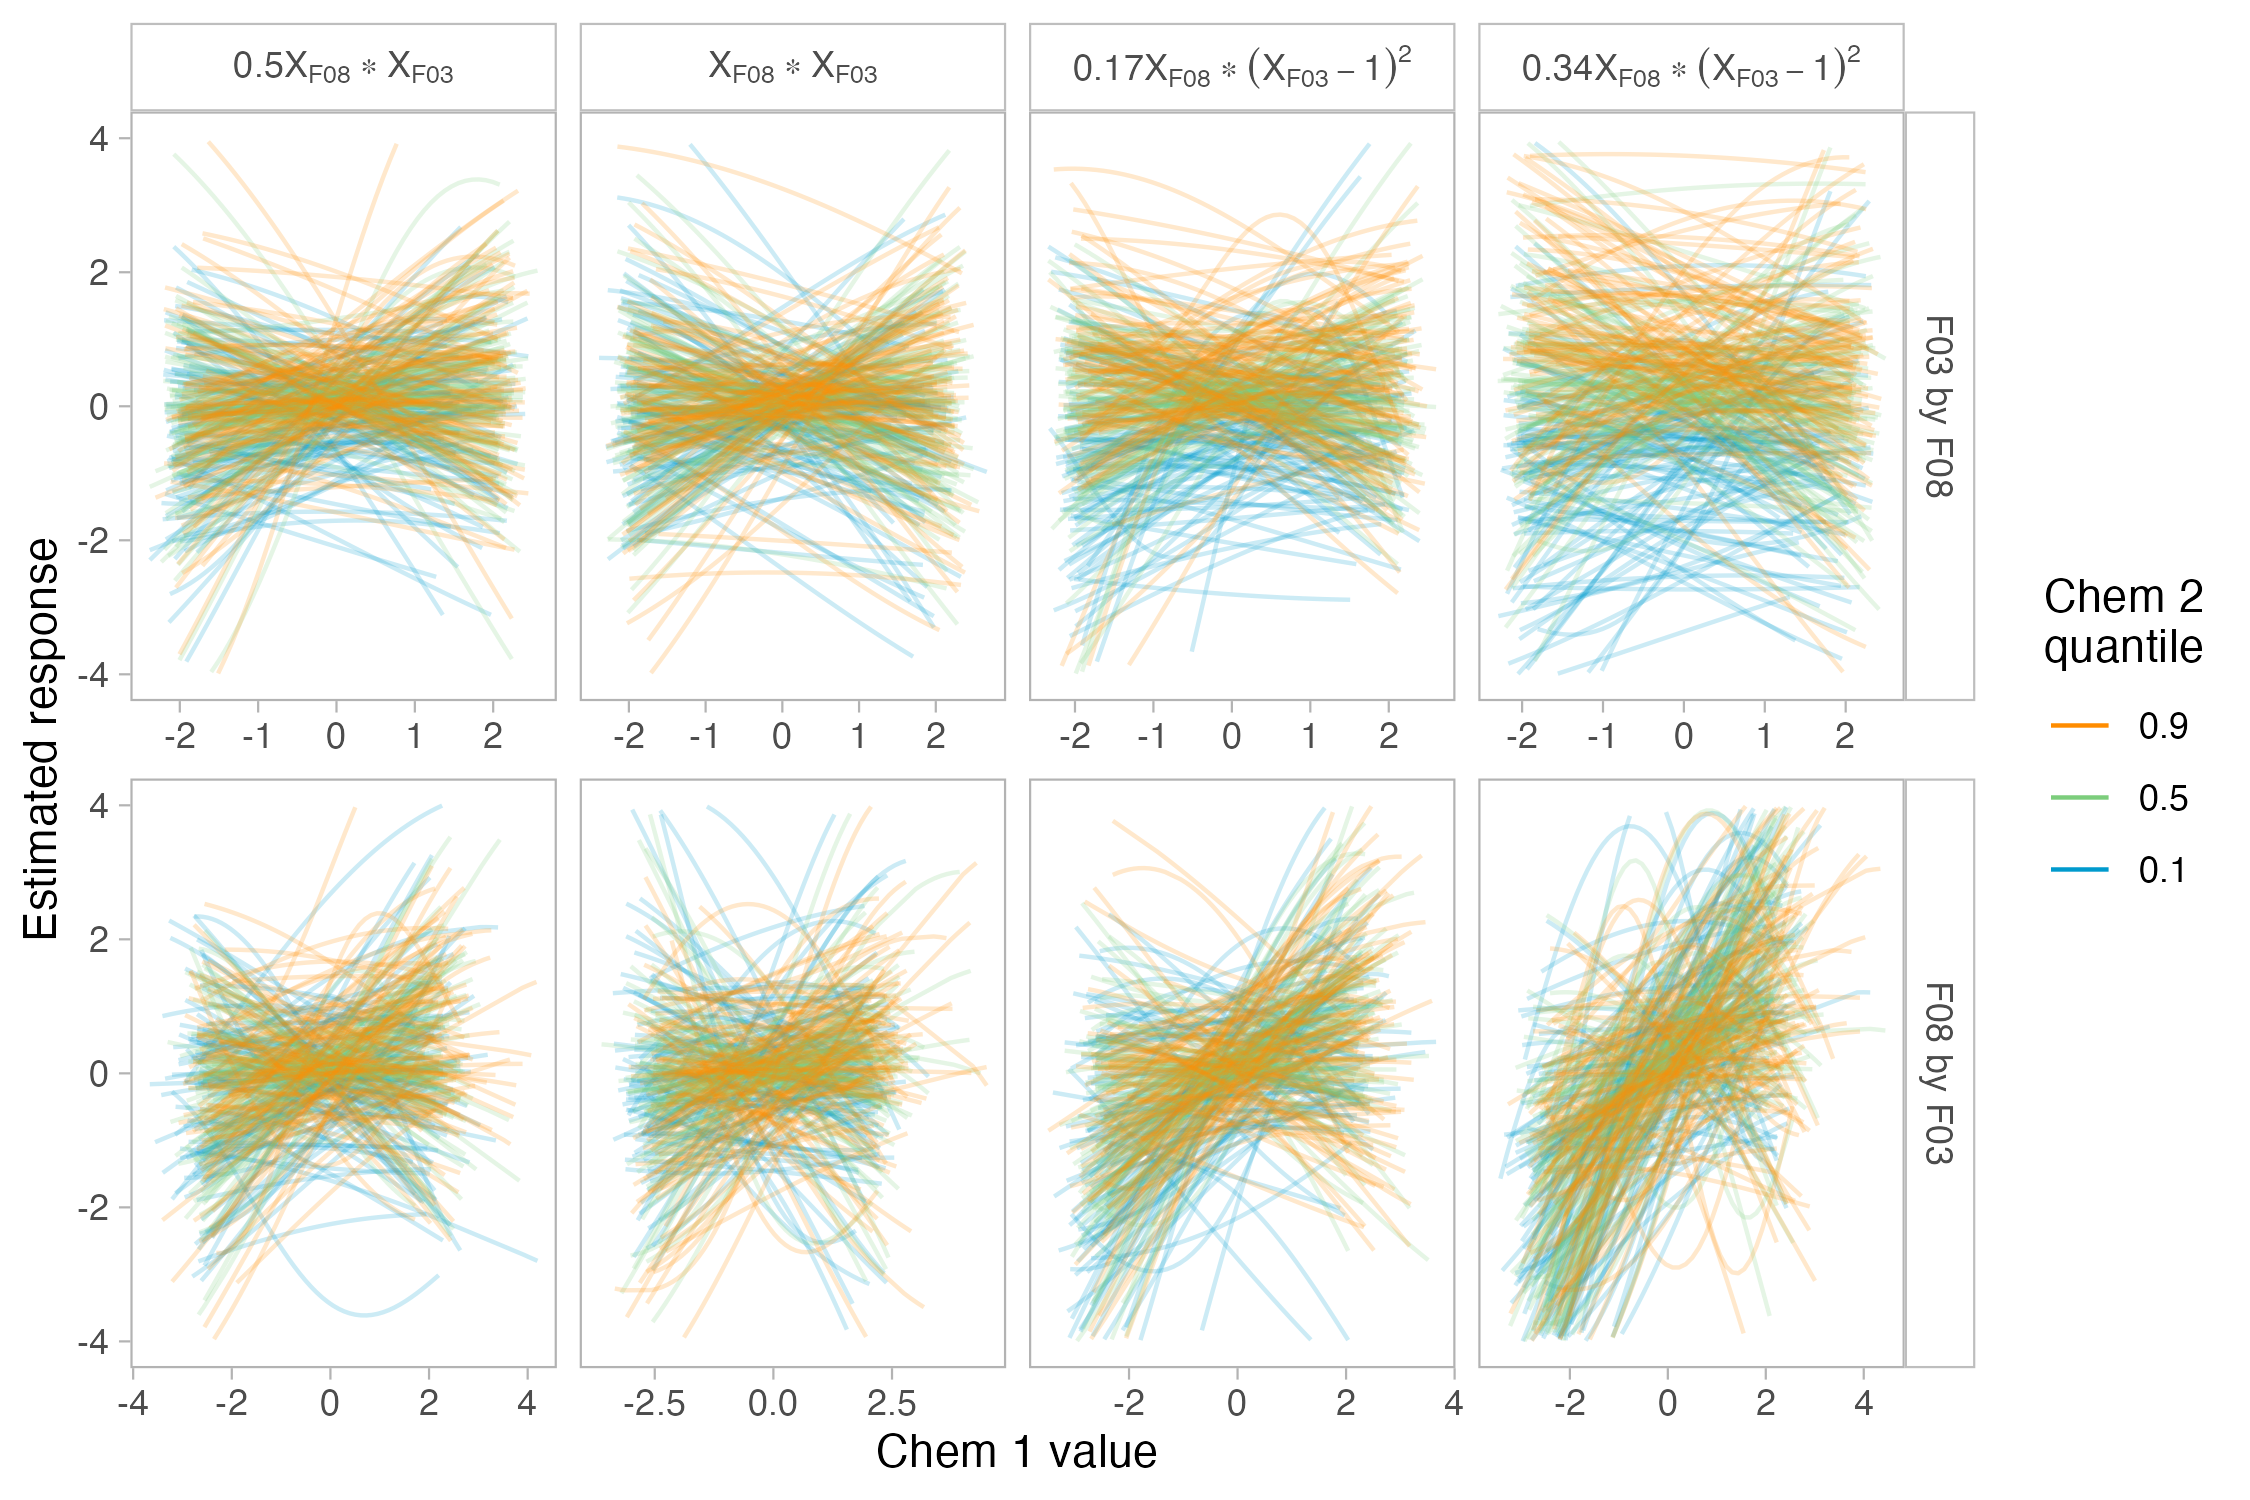
\includegraphics[width=0.8\linewidth]{figures/ch4_ksm_biv_expresp_2} 

}

\caption{Exposure-response relationships estimated by BKMR in smaller size (n=252) datasets, using the first chemical fixed at quantiles of another to assess interactions between Cd and As. All other chemicals are fixed at 0.5 quantiles.}\label{fig:ksmcdas}
\end{figure}
\begin{figure}

{\centering \includegraphics[width=0.8\linewidth]{figures/ch4_ssm_biv_expresp_2} 

}

\caption{Exposure-response relationships estimated by BSR in smaller size (n=252) datasets, using the first chemical fixed at quantiles of another to assess interactions between Cd and As. All other chemicals are fixed at 0.5 quantiles.}\label{fig:ssmcdas}
\end{figure}
\begin{figure}

{\centering \includegraphics[width=0.8\linewidth]{figures/ch4_klg_biv_expresp_2} 

}

\caption{Exposure-response relationships estimated by BKMR in larger size (n=1000) datasets, using the first chemical fixed at quantiles of another to assess interactions between Cd and As. All other chemicals are fixed at 0.5 quantiles.}\label{fig:klgcdas}
\end{figure}
\begin{figure}

{\centering \includegraphics[width=0.8\linewidth]{figures/ch4_slg_biv_expresp_2} 

}

\caption{Exposure-response relationships estimated by BSR in larger size (n=1000) datasets, using the first chemical fixed at quantiles of another to assess interactions between Cd and As. All other chemicals are fixed at 0.5 quantiles.}\label{fig:slgcdas}
\end{figure}
\begin{figure}

{\centering \includegraphics[width=0.8\linewidth]{figures/ch4_ksm_biv_expresp_3} 

}

\caption{Exposure-response relationships estimated by BKMR in smaller size (n=252) datasets, using the first chemical fixed at quantiles of another to assess interactions between Ni and Co. All other chemicals are fixed at 0.5 quantiles.}\label{fig:ksmnico}
\end{figure}
\begin{figure}

{\centering \includegraphics[width=0.8\linewidth]{figures/ch4_ssm_biv_expresp_3} 

}

\caption{Exposure-response relationships estimated by BSR in smaller size (n=252) datasets, using the first chemical fixed at quantiles of another to assess interactions between Ni and Co. All other chemicals are fixed at 0.5 quantiles.}\label{fig:ssmnico}
\end{figure}
\begin{figure}

{\centering \includegraphics[width=0.8\linewidth]{figures/ch4_klg_biv_expresp_3} 

}

\caption{Exposure-response relationships estimated by BKMR in larger size (n=1000) datasets, using the first chemical fixed at quantiles of another to assess interactions between Ni and Co. All other chemicals are fixed at 0.5 quantiles.}\label{fig:klgnico}
\end{figure}
\begin{figure}

{\centering \includegraphics[width=0.8\linewidth]{figures/ch4_slg_biv_expresp_3} 

}

\caption{Exposure-response relationships estimated by BSR in larger size (n=1000) datasets, using the first chemical fixed at quantiles of another to assess interactions between Ni and Co. All other chemicals are fixed at 0.5 quantiles.}\label{fig:slgnico}
\end{figure}
\begin{figure}

{\centering \includegraphics[width=0.8\linewidth]{figures/ch4_ksm_triv_expresp} 

}

\caption{Exposure-response relationships estimated by BKMR in smaller size (n=252) datasets, using the first chemical fixed at quantiles of two others to assess interactions between Ni, Hg, and Tl. All other chemicals are fixed at 0.5 quantiles.}\label{fig:ksmtri}
\end{figure}
\begin{figure}

{\centering \includegraphics[width=0.8\linewidth]{figures/ch4_ssm_triv_expresp} 

}

\caption{Exposure-response relationships estimated by BSR in smaller size (n=252) datasets, using the first chemical fixed at quantiles of two others to assess interactions between Ni, Hg, and Tl. All other chemicals are fixed at 0.5 quantiles.}\label{fig:ssmtri}
\end{figure}
\begin{figure}

{\centering \includegraphics[width=0.8\linewidth]{figures/ch4_klg_triv_expresp} 

}

\caption{Exposure-response relationships estimated by BKMR in larger size (n=1000) datasets, using the first chemical fixed at quantiles of two others to assess interactions between Ni, Hg, and Tl. All other chemicals are fixed at 0.5 quantiles.}\label{fig:klgtri}
\end{figure}
\begin{figure}

{\centering \includegraphics[width=0.8\linewidth]{figures/ch4_slg_triv_expresp} 

}

\caption{Exposure-response relationships estimated by BSR in larger size (n=1000) datasets, using the first chemical fixed at quantiles of two others to assess interactions between Ni, Hg, and Tl. All other chemicals are fixed at 0.5 quantiles.}\label{fig:slgtri}
\end{figure}
Table \ref{tab:reunivsens} summarizes the sensitivities for Hg in scenarios with interactions between the categorical race covariate and Hg. Note that the naive and oracle MLRs do not have an associated race category, because we did not stratify them in our analysis.
\begin{table}

\caption{\label{tab:reunivsens}Sensitivity for the univariate Hg term in all scenarios with an interaction between the categorical race covariate and Hg. Sensitivities for BKMR and BSR models are stratified by race.}
\centering
\begin{tabular}[t]{llcccc}
\toprule
\multicolumn{2}{c}{\textbf{ }} & \multicolumn{2}{c}{\textbf{Small race cat.}} & \multicolumn{2}{c}{\textbf{Large race cat.}} \\
\cmidrule(l{3pt}r{3pt}){3-4} \cmidrule(l{3pt}r{3pt}){5-6}
Model & Race & Lower & Higher & Lower & Higher\\
\midrule
\addlinespace[0.3em]
\multicolumn{6}{l}{\textbf{Small}}\\
\hspace{1em}Naive MLR & - & 0.84 & 0.79 & 0.93 & 0.99\\
\addlinespace
\hspace{1em}Oracle MLR & - & 0.82 & 0.78 & 0.70 & 0.56\\
\addlinespace
 & Non-Hisp. white (n=16) & 0.52 & 0.47 & 0.42 & 0.51\\

 & Non-Hisp. black (n=27) & 0.60 & 0.69 & 0.50 & 0.56\\

 & Non-Hisp. other (n=13) & 0.30 & 0.27 & 0.27 & 0.20\\

 & Hisp. born in US (n=87) & 0.56 & 0.50 & 0.57 & 0.60\\

 & Hisp. born outside US (n=109) & 0.68 & 0.63 & 0.89 & 0.97\\

\multirow{-6}{*}{\raggedright\arraybackslash \hspace{1em}BKMR} & Collapsed non-Hisp. (n=56) & 0.54 & 0.65 & 0.55 & 0.46\\
\addlinespace
 & Non-Hisp. white (n=16) & 0.32 & 0.30 & 0.42 & 0.40\\

 & Non-Hisp. black (n=27) & 0.26 & 0.41 & 0.22 & 0.23\\

 & Non-Hisp. other (n=13) & 0.36 & 0.35 & 0.32 & 0.40\\

 & Hisp. born in US (n=87) & 0.23 & 0.15 & 0.13 & 0.18\\

 & Hisp. born outside US (n=109) & 0.23 & 0.25 & 0.53 & 0.80\\

\multirow{-6}{*}{\raggedright\arraybackslash \hspace{1em}BSR} & Collapsed non-Hisp. (n=56) & 0.17 & 0.33 & 0.23 & 0.16\\
\addlinespace
\addlinespace[0.3em]
\multicolumn{6}{l}{\textbf{Large}}\\
\hspace{1em}Naive MLR & - & 1.00 & 1.00 & 1.00 & 1.00\\
\addlinespace
\hspace{1em}Oracle MLR & - & 1.00 & 1.00 & 0.99 & 1.00\\
\addlinespace
 & Non-Hisp. white (n=16) & 0.45 & 0.56 & 0.50 & 0.43\\

 & Non-Hisp. black (n=27) & 0.88 & 0.93 & 0.59 & 0.59\\

 & Non-Hisp. other (n=13) & 0.55 & 0.41 & 0.52 & 0.53\\

 & Hisp. born in US (n=87) & 0.90 & 0.93 & 0.88 & 0.95\\

\multirow{-5}{*}{\raggedright\arraybackslash \hspace{1em}BKMR} & Hisp. born outside US (n=109) & 0.92 & 0.94 & 1.00 & 1.00\\
\addlinespace
 & Non-Hisp. white (n=16) & 0.16 & 0.18 & 0.18 & 0.13\\

 & Non-Hisp. black (n=27) & 0.56 & 0.82 & 0.24 & 0.30\\

 & Non-Hisp. other (n=13) & 0.17 & 0.11 & 0.18 & 0.17\\

 & Hisp. born in US (n=87) & 0.76 & 0.70 & 0.71 & 0.70\\

\multirow{-5}{*}{\raggedright\arraybackslash \hspace{1em}BSR} & Hisp. born outside US (n=109) & 0.79 & 0.85 & 1.00 & 1.00\\
\bottomrule
\end{tabular}
\end{table}
\hypertarget{code}{%
\chapter{Code}\label{code}}

This second appendix includes all of the R chunks of code that were hidden throughout the document.

\hypertarget{code-for-chapter-refbayes}{%
\section{Code for Chapter \ref{bayes}:}\label{code-for-chapter-refbayes}}

The code for this section generates a toy example, used to demonstrate the kernel machine regression and spline regression techniques.

\scriptsize
\begin{Shaded}
\begin{Highlighting}[]
\CommentTok{\#load packages}
\FunctionTok{library}\NormalTok{(tidyverse)}
\FunctionTok{library}\NormalTok{(stats)}
\FunctionTok{library}\NormalTok{(splines)}
\end{Highlighting}
\end{Shaded}
\normalsize

\scriptsize
\begin{Shaded}
\begin{Highlighting}[]
\CommentTok{\# set theme for plots}
\FunctionTok{theme\_set}\NormalTok{(}\FunctionTok{theme\_light}\NormalTok{())}
\FunctionTok{theme\_update}\NormalTok{(}\AttributeTok{panel.grid.major =} \FunctionTok{element\_blank}\NormalTok{(), }
             \AttributeTok{panel.grid.minor =} \FunctionTok{element\_blank}\NormalTok{())}
\FunctionTok{theme\_update}\NormalTok{(}
  \AttributeTok{strip.background =} \FunctionTok{element\_rect}\NormalTok{(}\AttributeTok{color=}\StringTok{"gray"}\NormalTok{, }\AttributeTok{fill=}\StringTok{"white"}\NormalTok{), }
  \AttributeTok{strip.text =} \FunctionTok{element\_text}\NormalTok{(}\AttributeTok{color =} \StringTok{"gray30"}\NormalTok{)}
\NormalTok{  )}
\end{Highlighting}
\end{Shaded}
\normalsize

\scriptsize
\begin{Shaded}
\begin{Highlighting}[]
\DocumentationTok{\#\#\#\#\#\#\#\#}
\CommentTok{\# generate simulated points}
\DocumentationTok{\#\#\#\#\#\#\#\#}

\CommentTok{\# generate data from distribution}
\FunctionTok{set.seed}\NormalTok{(}\DecValTok{0}\NormalTok{) }\CommentTok{\# reproducibility}
\NormalTok{x }\OtherTok{\textless{}{-}} \FunctionTok{seq}\NormalTok{(}\DecValTok{0}\NormalTok{, }\DecValTok{25}\NormalTok{, }\AttributeTok{length.out =} \DecValTok{51}\NormalTok{)}
\NormalTok{Y }\OtherTok{\textless{}{-}} \FunctionTok{exp}\NormalTok{(x}\SpecialCharTok{/}\DecValTok{10}\NormalTok{) }\SpecialCharTok{+} \DecValTok{2}\SpecialCharTok{*}\FunctionTok{sin}\NormalTok{(x}\SpecialCharTok{/}\DecValTok{2}\NormalTok{) }\SpecialCharTok{+} \FunctionTok{rnorm}\NormalTok{(}\DecValTok{51}\NormalTok{, }\AttributeTok{mean =} \DecValTok{0}\NormalTok{, }\AttributeTok{sd =} \FloatTok{0.5}\NormalTok{)}
\NormalTok{df }\OtherTok{\textless{}{-}} \FunctionTok{data.frame}\NormalTok{(x, Y)}

\CommentTok{\# plot data and linear regression line}
\NormalTok{q1 }\OtherTok{\textless{}{-}} \FunctionTok{ggplot}\NormalTok{(df, }\FunctionTok{aes}\NormalTok{(x, Y)) }\SpecialCharTok{+}
  \FunctionTok{geom\_point}\NormalTok{() }\SpecialCharTok{+}
  \FunctionTok{geom\_function}\NormalTok{(}\AttributeTok{fun =} \ControlFlowTok{function}\NormalTok{(x) }\FunctionTok{exp}\NormalTok{(x}\SpecialCharTok{/}\DecValTok{10}\NormalTok{) }\SpecialCharTok{+} \DecValTok{2}\SpecialCharTok{*}\FunctionTok{sin}\NormalTok{(x}\SpecialCharTok{/}\DecValTok{2}\NormalTok{), }
                \AttributeTok{linetype =} \StringTok{"dashed"}\NormalTok{, }\AttributeTok{color =} \StringTok{"darkorange"}\NormalTok{) }\SpecialCharTok{+} 
  \FunctionTok{geom\_smooth}\NormalTok{(}\AttributeTok{method =} \StringTok{"lm"}\NormalTok{, }\AttributeTok{formula =} \StringTok{"y\textasciitilde{}x"}\NormalTok{, }
              \AttributeTok{color =} \StringTok{"deepskyblue3"}\NormalTok{, }\AttributeTok{fill =} \StringTok{"gray70"}\NormalTok{, }
              \AttributeTok{linewidth =} \FloatTok{0.5}\NormalTok{, }\AttributeTok{se =}\NormalTok{ F)}

\CommentTok{\# save plot}
\FunctionTok{ggsave}\NormalTok{(}\StringTok{"index/figures/ch3\_toy1.png"}\NormalTok{, }\AttributeTok{plot =}\NormalTok{ q1, }\AttributeTok{device =} \StringTok{"png"}\NormalTok{, }
       \AttributeTok{width =} \DecValTok{5}\NormalTok{, }\AttributeTok{height =} \DecValTok{3}\NormalTok{)}
\end{Highlighting}
\end{Shaded}
\normalsize

\scriptsize
\begin{Shaded}
\begin{Highlighting}[]
\DocumentationTok{\#\#\#\#\#\#\#\#}
\CommentTok{\# kernel regression}
\DocumentationTok{\#\#\#\#\#\#\#\#}

\CommentTok{\# get normal distribution of weights around query points}
\NormalTok{df}\SpecialCharTok{$}\NormalTok{Weight }\OtherTok{\textless{}{-}} \FunctionTok{dnorm}\NormalTok{(df}\SpecialCharTok{$}\NormalTok{x, }\AttributeTok{mean =} \FloatTok{12.5}\NormalTok{, }\AttributeTok{sd =} \DecValTok{1}\NormalTok{)}

\CommentTok{\# plot points colored by their weights}
\NormalTok{p1 }\OtherTok{\textless{}{-}} \FunctionTok{ggplot}\NormalTok{(df, }\FunctionTok{aes}\NormalTok{(x, Y)) }\SpecialCharTok{+}
  \FunctionTok{geom\_point}\NormalTok{(}\FunctionTok{aes}\NormalTok{(}\AttributeTok{color =}\NormalTok{ Weight)) }\SpecialCharTok{+}
  \FunctionTok{geom\_function}\NormalTok{(}\AttributeTok{fun =} \ControlFlowTok{function}\NormalTok{(x) }\FunctionTok{exp}\NormalTok{(x}\SpecialCharTok{/}\DecValTok{10}\NormalTok{) }\SpecialCharTok{+} \DecValTok{2}\SpecialCharTok{*}\FunctionTok{sin}\NormalTok{(x}\SpecialCharTok{/}\DecValTok{2}\NormalTok{), }
                \AttributeTok{linetype =} \StringTok{"dashed"}\NormalTok{, }\AttributeTok{color =} \StringTok{"darkorange"}\NormalTok{) }\SpecialCharTok{+} 
  \FunctionTok{geom\_vline}\NormalTok{(}\AttributeTok{xintercept =} \FloatTok{12.5}\NormalTok{, }\AttributeTok{linetype =} \StringTok{"dotted"}\NormalTok{) }\SpecialCharTok{+}
  \FunctionTok{theme}\NormalTok{(}\AttributeTok{legend.position =} \StringTok{"none"}\NormalTok{)}

\CommentTok{\# plot a curve of weights}
\NormalTok{normcurv }\OtherTok{\textless{}{-}} \FunctionTok{data.frame}\NormalTok{(}\AttributeTok{x =} \FunctionTok{seq}\NormalTok{(}\DecValTok{0}\NormalTok{, }\DecValTok{25}\NormalTok{, }\AttributeTok{length.out =} \DecValTok{250}\NormalTok{)) }
\NormalTok{normcurv}\SpecialCharTok{$}\NormalTok{Weight }\OtherTok{\textless{}{-}} \FunctionTok{dnorm}\NormalTok{(normcurv}\SpecialCharTok{$}\NormalTok{x, }\AttributeTok{mean =} \FloatTok{12.5}\NormalTok{, }\AttributeTok{sd =} \DecValTok{1}\NormalTok{)}
\NormalTok{p2 }\OtherTok{\textless{}{-}} \FunctionTok{ggplot}\NormalTok{(normcurv, }\FunctionTok{aes}\NormalTok{(x, Weight, }\AttributeTok{color =}\NormalTok{ Weight)) }\SpecialCharTok{+}
  \FunctionTok{geom\_line}\NormalTok{() }\SpecialCharTok{+}
  \FunctionTok{scale\_y\_continuous}\NormalTok{(}\AttributeTok{breaks =} \FunctionTok{c}\NormalTok{(}\DecValTok{0}\NormalTok{, }\FloatTok{0.2}\NormalTok{, }\FloatTok{0.4}\NormalTok{)) }\SpecialCharTok{+}
  \FunctionTok{theme}\NormalTok{(}\AttributeTok{legend.position =} \StringTok{"none"}\NormalTok{) }

\CommentTok{\# stitch plots together}
\NormalTok{q2 }\OtherTok{\textless{}{-}}\NormalTok{ cowplot}\SpecialCharTok{::}\FunctionTok{plot\_grid}\NormalTok{(p1, p2, }\AttributeTok{ncol =} \DecValTok{1}\NormalTok{, }\AttributeTok{rel\_heights =} \FunctionTok{c}\NormalTok{(}\FloatTok{0.7}\NormalTok{, }\FloatTok{0.3}\NormalTok{))}
\NormalTok{q2}

\CommentTok{\# save plot}
\FunctionTok{ggsave}\NormalTok{(}\StringTok{"index/figures/ch3\_toy2.png"}\NormalTok{, }\AttributeTok{plot =}\NormalTok{ q2, }\AttributeTok{device =} \StringTok{"png"}\NormalTok{, }
       \AttributeTok{width =} \DecValTok{5}\NormalTok{, }\AttributeTok{height =} \DecValTok{4}\NormalTok{)}

\CommentTok{\# fit kernel regression with sigma = 1, bandwidth = 8/3}
\NormalTok{kmr\_toy }\OtherTok{\textless{}{-}} \FunctionTok{ksmooth}\NormalTok{(df}\SpecialCharTok{$}\NormalTok{x, df}\SpecialCharTok{$}\NormalTok{Y, }\AttributeTok{kernel =} \StringTok{"normal"}\NormalTok{, }
                   \AttributeTok{bandwidth =} \DecValTok{8}\SpecialCharTok{/}\DecValTok{3}\NormalTok{, }\AttributeTok{x.points =}\NormalTok{ df}\SpecialCharTok{$}\NormalTok{x)}
\NormalTok{df }\OtherTok{\textless{}{-}}\NormalTok{ df }\SpecialCharTok{|\textgreater{}} 
  \FunctionTok{left\_join}\NormalTok{(}\FunctionTok{as.data.frame}\NormalTok{(kmr\_toy), }\AttributeTok{by =} \StringTok{"x"}\NormalTok{) }\SpecialCharTok{|\textgreater{}} 
  \FunctionTok{rename}\NormalTok{(}\AttributeTok{Yhat =}\NormalTok{ y)}

\CommentTok{\# plot kernel regression estimation}
\NormalTok{q3 }\OtherTok{\textless{}{-}} \FunctionTok{ggplot}\NormalTok{(df) }\SpecialCharTok{+}
  \FunctionTok{geom\_point}\NormalTok{(}\FunctionTok{aes}\NormalTok{(x, Y)) }\SpecialCharTok{+}
  \FunctionTok{geom\_function}\NormalTok{(}\AttributeTok{fun =} \ControlFlowTok{function}\NormalTok{(x) }\FunctionTok{exp}\NormalTok{(x}\SpecialCharTok{/}\DecValTok{10}\NormalTok{) }\SpecialCharTok{+} \DecValTok{2}\SpecialCharTok{*}\FunctionTok{sin}\NormalTok{(x}\SpecialCharTok{/}\DecValTok{2}\NormalTok{), }
                \AttributeTok{linetype =} \StringTok{"dashed"}\NormalTok{, }\AttributeTok{color =} \StringTok{"darkorange"}\NormalTok{) }\SpecialCharTok{+}
  \FunctionTok{geom\_line}\NormalTok{(}\FunctionTok{aes}\NormalTok{(x, Yhat), }\AttributeTok{color =} \StringTok{"deepskyblue3"}\NormalTok{) }
\NormalTok{q3}

\CommentTok{\# save plot}
\FunctionTok{ggsave}\NormalTok{(}\StringTok{"index/figures/ch3\_toy3.png"}\NormalTok{, }\AttributeTok{plot =}\NormalTok{ q3, }\AttributeTok{device =} \StringTok{"png"}\NormalTok{, }
       \AttributeTok{width =} \DecValTok{5}\NormalTok{, }\AttributeTok{height =} \DecValTok{3}\NormalTok{)}

\CommentTok{\# fit kernel regression with sigma = 5, bandwidth = 40/3}
\NormalTok{kmr\_toy\_5 }\OtherTok{\textless{}{-}} \FunctionTok{ksmooth}\NormalTok{(df}\SpecialCharTok{$}\NormalTok{x, df}\SpecialCharTok{$}\NormalTok{Y, }\AttributeTok{kernel =} \StringTok{"normal"}\NormalTok{, }
                     \AttributeTok{bandwidth =} \DecValTok{40}\SpecialCharTok{/}\DecValTok{3}\NormalTok{, }\AttributeTok{x.points =}\NormalTok{ df}\SpecialCharTok{$}\NormalTok{x)}

\CommentTok{\# fit kernel regression with sigma = 0.1, bandwith = 8/30}
\NormalTok{kmr\_toy\_1 }\OtherTok{\textless{}{-}} \FunctionTok{ksmooth}\NormalTok{(df}\SpecialCharTok{$}\NormalTok{x, df}\SpecialCharTok{$}\NormalTok{Y, }\AttributeTok{kernel =} \StringTok{"normal"}\NormalTok{, }
                     \AttributeTok{bandwidth =} \DecValTok{8}\SpecialCharTok{/}\DecValTok{30}\NormalTok{, }\AttributeTok{x.points =}\NormalTok{ df}\SpecialCharTok{$}\NormalTok{x)}

\CommentTok{\# re{-}join data}
\NormalTok{dfrho }\OtherTok{\textless{}{-}}\NormalTok{ df }\SpecialCharTok{|\textgreater{}} 
  \FunctionTok{left\_join}\NormalTok{(}\FunctionTok{as.data.frame}\NormalTok{(kmr\_toy\_5), }\AttributeTok{by =} \StringTok{"x"}\NormalTok{) }\SpecialCharTok{|\textgreater{}} 
  \FunctionTok{rename}\NormalTok{(}\StringTok{"rho = 50"} \OtherTok{=}\NormalTok{ y) }\SpecialCharTok{|\textgreater{}} 
  \FunctionTok{left\_join}\NormalTok{(}\FunctionTok{as.data.frame}\NormalTok{(kmr\_toy\_1), }\AttributeTok{by =} \StringTok{"x"}\NormalTok{) }\SpecialCharTok{|\textgreater{}} 
  \FunctionTok{rename}\NormalTok{(}\StringTok{"rho = 0.02"} \OtherTok{=}\NormalTok{ y) }\SpecialCharTok{|\textgreater{}} 
  \FunctionTok{select}\NormalTok{(}\SpecialCharTok{{-}}\NormalTok{Yhat) }\SpecialCharTok{|\textgreater{}} 
  \FunctionTok{pivot\_longer}\NormalTok{(}\AttributeTok{cols =} \FunctionTok{c}\NormalTok{(}\StringTok{"rho = 50"}\NormalTok{, }\StringTok{"rho = 0.02"}\NormalTok{), }\AttributeTok{values\_to =} \StringTok{"Yhat"}\NormalTok{)}

\CommentTok{\# plot kernel regression with two values of rho}
\NormalTok{qrho }\OtherTok{\textless{}{-}} \FunctionTok{ggplot}\NormalTok{(dfrho) }\SpecialCharTok{+}
  \FunctionTok{geom\_point}\NormalTok{(}\FunctionTok{aes}\NormalTok{(x, Y)) }\SpecialCharTok{+}
  \FunctionTok{geom\_line}\NormalTok{(}\FunctionTok{aes}\NormalTok{(x, Yhat), }\AttributeTok{color =} \StringTok{"deepskyblue3"}\NormalTok{) }\SpecialCharTok{+}
  \FunctionTok{facet\_wrap}\NormalTok{(}\SpecialCharTok{\textasciitilde{}}\NormalTok{name)}
\NormalTok{qrho}

\CommentTok{\# save plot}
\FunctionTok{ggsave}\NormalTok{(}\StringTok{"index/figures/ch3\_toyrho.png"}\NormalTok{, }\AttributeTok{plot =}\NormalTok{ qrho, }\AttributeTok{device =} \StringTok{"png"}\NormalTok{, }
       \AttributeTok{width =} \DecValTok{7}\NormalTok{, }\AttributeTok{height =} \DecValTok{3}\NormalTok{)}
\end{Highlighting}
\end{Shaded}
\normalsize

\scriptsize
\begin{Shaded}
\begin{Highlighting}[]
\DocumentationTok{\#\#\#\#\#\#\#\#}
\CommentTok{\# spline regression}
\DocumentationTok{\#\#\#\#\#\#\#\#}

\NormalTok{kn }\OtherTok{\textless{}{-}} \FunctionTok{c}\NormalTok{(}\DecValTok{5}\NormalTok{, }\DecValTok{10}\NormalTok{, }\DecValTok{15}\NormalTok{, }\DecValTok{20}\NormalTok{) }\CommentTok{\# 4 knots of equal width}

\CommentTok{\# fit linear spline regression}
\NormalTok{spline\_toy\_line }\OtherTok{\textless{}{-}} \FunctionTok{lm}\NormalTok{(Y }\SpecialCharTok{\textasciitilde{}} \FunctionTok{bs}\NormalTok{(x, }\AttributeTok{knots =}\NormalTok{ kn, }\AttributeTok{degree =} \DecValTok{1}\NormalTok{), }\AttributeTok{data =}\NormalTok{ df)}
\NormalTok{p\_line }\OtherTok{\textless{}{-}} \FunctionTok{predict}\NormalTok{(spline\_toy\_line, }\AttributeTok{se =}\NormalTok{ T)}
\NormalTok{df}\SpecialCharTok{$}\NormalTok{Yhats\_line }\OtherTok{\textless{}{-}}\NormalTok{ p\_line}\SpecialCharTok{$}\NormalTok{fit}

\NormalTok{q4 }\OtherTok{\textless{}{-}} \FunctionTok{ggplot}\NormalTok{(df) }\SpecialCharTok{+}
  \FunctionTok{geom\_point}\NormalTok{(}\FunctionTok{aes}\NormalTok{(x, Y)) }\SpecialCharTok{+}
  \FunctionTok{geom\_function}\NormalTok{(}\AttributeTok{fun =} \ControlFlowTok{function}\NormalTok{(x) }\FunctionTok{exp}\NormalTok{(x}\SpecialCharTok{/}\DecValTok{10}\NormalTok{) }\SpecialCharTok{+} \DecValTok{2}\SpecialCharTok{*}\FunctionTok{sin}\NormalTok{(x}\SpecialCharTok{/}\DecValTok{2}\NormalTok{), }
                \AttributeTok{linetype =} \StringTok{"dashed"}\NormalTok{, }\AttributeTok{color =} \StringTok{"darkorange"}\NormalTok{) }\SpecialCharTok{+}
  \FunctionTok{geom\_line}\NormalTok{(}\FunctionTok{aes}\NormalTok{(x, Yhats\_line), }\AttributeTok{color =} \StringTok{"deepskyblue3"}\NormalTok{) }\SpecialCharTok{+}
  \FunctionTok{geom\_vline}\NormalTok{(}\AttributeTok{xintercept =}\NormalTok{ kn, }\AttributeTok{linetype =} \StringTok{"dotted"}\NormalTok{)}
\NormalTok{q4}

\CommentTok{\# save plot}
\FunctionTok{ggsave}\NormalTok{(}\StringTok{"index/figures/ch3\_toy4.png"}\NormalTok{, }\AttributeTok{plot =}\NormalTok{ q4, }\AttributeTok{device =} \StringTok{"png"}\NormalTok{, }
       \AttributeTok{width =} \DecValTok{5}\NormalTok{, }\AttributeTok{height =} \DecValTok{3}\NormalTok{)}

\CommentTok{\# fit cubic spline regression}
\NormalTok{spline\_toy\_cub }\OtherTok{\textless{}{-}} \FunctionTok{lm}\NormalTok{(Y }\SpecialCharTok{\textasciitilde{}} \FunctionTok{bs}\NormalTok{(x, }\AttributeTok{knots =}\NormalTok{ kn), }\AttributeTok{data =}\NormalTok{ df)}
\NormalTok{p\_cub }\OtherTok{\textless{}{-}} \FunctionTok{predict}\NormalTok{(spline\_toy\_cub, }\AttributeTok{se =}\NormalTok{ T)}
\NormalTok{df}\SpecialCharTok{$}\NormalTok{Yhats\_cub }\OtherTok{\textless{}{-}}\NormalTok{ p\_cub}\SpecialCharTok{$}\NormalTok{fit}

\CommentTok{\# plot spline regression estimation}
\NormalTok{q5 }\OtherTok{\textless{}{-}} \FunctionTok{ggplot}\NormalTok{(df) }\SpecialCharTok{+}
  \FunctionTok{geom\_point}\NormalTok{(}\FunctionTok{aes}\NormalTok{(x, Y)) }\SpecialCharTok{+}
  \FunctionTok{geom\_function}\NormalTok{(}\AttributeTok{fun =} \ControlFlowTok{function}\NormalTok{(x) }\FunctionTok{exp}\NormalTok{(x}\SpecialCharTok{/}\DecValTok{10}\NormalTok{) }\SpecialCharTok{+} \DecValTok{2}\SpecialCharTok{*}\FunctionTok{sin}\NormalTok{(x}\SpecialCharTok{/}\DecValTok{2}\NormalTok{), }
                \AttributeTok{linetype =} \StringTok{"dashed"}\NormalTok{, }\AttributeTok{color =} \StringTok{"darkorange"}\NormalTok{) }\SpecialCharTok{+}
  \FunctionTok{geom\_line}\NormalTok{(}\FunctionTok{aes}\NormalTok{(x, Yhats\_cub), }\AttributeTok{color =} \StringTok{"deepskyblue3"}\NormalTok{) }\SpecialCharTok{+}
  \FunctionTok{geom\_vline}\NormalTok{(}\AttributeTok{xintercept =}\NormalTok{ kn, }\AttributeTok{linetype =} \StringTok{"dotted"}\NormalTok{)}
\NormalTok{q5}

\CommentTok{\# save plot}
\FunctionTok{ggsave}\NormalTok{(}\StringTok{"index/figures/ch3\_toy5.png"}\NormalTok{, }\AttributeTok{plot =}\NormalTok{ q5, }\AttributeTok{device =} \StringTok{"png"}\NormalTok{, }
       \AttributeTok{width =} \DecValTok{5}\NormalTok{, }\AttributeTok{height =} \DecValTok{3}\NormalTok{)}

\CommentTok{\# fit natural spline regression}
\NormalTok{spline\_toy\_nat }\OtherTok{\textless{}{-}} \FunctionTok{lm}\NormalTok{(Y }\SpecialCharTok{\textasciitilde{}} \FunctionTok{ns}\NormalTok{(x, }\AttributeTok{knots =}\NormalTok{ kn), }\AttributeTok{data =}\NormalTok{ df)}
\NormalTok{p\_nat }\OtherTok{\textless{}{-}} \FunctionTok{predict}\NormalTok{(spline\_toy\_nat, }\AttributeTok{se =}\NormalTok{ T)}
\NormalTok{df}\SpecialCharTok{$}\NormalTok{Yhats\_nat }\OtherTok{\textless{}{-}}\NormalTok{ p\_nat}\SpecialCharTok{$}\NormalTok{fit}

\CommentTok{\# plot spline regression estimation}
\NormalTok{q6 }\OtherTok{\textless{}{-}} \FunctionTok{ggplot}\NormalTok{(df) }\SpecialCharTok{+}
  \FunctionTok{geom\_point}\NormalTok{(}\FunctionTok{aes}\NormalTok{(x, Y)) }\SpecialCharTok{+}
  \FunctionTok{geom\_function}\NormalTok{(}\AttributeTok{fun =} \ControlFlowTok{function}\NormalTok{(x) }\FunctionTok{exp}\NormalTok{(x}\SpecialCharTok{/}\DecValTok{10}\NormalTok{) }\SpecialCharTok{+} \DecValTok{2}\SpecialCharTok{*}\FunctionTok{sin}\NormalTok{(x}\SpecialCharTok{/}\DecValTok{2}\NormalTok{), }
                \AttributeTok{linetype =} \StringTok{"dashed"}\NormalTok{, }\AttributeTok{color =} \StringTok{"darkorange"}\NormalTok{) }\SpecialCharTok{+}
  \FunctionTok{geom\_line}\NormalTok{(}\FunctionTok{aes}\NormalTok{(x, Yhats\_nat), }\AttributeTok{color =} \StringTok{"deepskyblue3"}\NormalTok{) }\SpecialCharTok{+}
  \FunctionTok{geom\_vline}\NormalTok{(}\AttributeTok{xintercept =} \FunctionTok{c}\NormalTok{(}\DecValTok{5}\NormalTok{, }\DecValTok{10}\NormalTok{, }\DecValTok{15}\NormalTok{, }\DecValTok{20}\NormalTok{), }\AttributeTok{linetype =} \StringTok{"dotted"}\NormalTok{)}
\NormalTok{q6}

\CommentTok{\# save plot}
\FunctionTok{ggsave}\NormalTok{(}\StringTok{"index/figures/ch3\_toy6.png"}\NormalTok{, }\AttributeTok{plot =}\NormalTok{ q6, }\AttributeTok{device =} \StringTok{"png"}\NormalTok{, }
       \AttributeTok{width =} \DecValTok{5}\NormalTok{, }\AttributeTok{height =} \DecValTok{3}\NormalTok{)}

\CommentTok{\# see what happens outside of the bounds}
\NormalTok{x\_longer }\OtherTok{\textless{}{-}} \FunctionTok{seq}\NormalTok{(}\SpecialCharTok{{-}}\DecValTok{5}\NormalTok{, }\DecValTok{30}\NormalTok{, }\AttributeTok{length.out =} \DecValTok{81}\NormalTok{)}
\NormalTok{y\_longer\_cub }\OtherTok{\textless{}{-}} \FunctionTok{predict}\NormalTok{(spline\_toy\_cub, }
                        \AttributeTok{newdata =} \FunctionTok{data.frame}\NormalTok{(}\AttributeTok{x =}\NormalTok{ x\_longer))}
\NormalTok{y\_longer\_nat }\OtherTok{\textless{}{-}} \FunctionTok{predict}\NormalTok{(spline\_toy\_nat, }
                        \AttributeTok{newdata =} \FunctionTok{data.frame}\NormalTok{(}\AttributeTok{x =}\NormalTok{ x\_longer))}

\NormalTok{df\_longer }\OtherTok{\textless{}{-}} \FunctionTok{data.frame}\NormalTok{(}
  \AttributeTok{x =} \FunctionTok{c}\NormalTok{(x\_longer, x\_longer), }
  \AttributeTok{spline =} \FunctionTok{c}\NormalTok{(}\FunctionTok{rep}\NormalTok{(}\StringTok{"Cubic"}\NormalTok{, }\DecValTok{81}\NormalTok{), }\FunctionTok{rep}\NormalTok{(}\StringTok{"Natural"}\NormalTok{, }\DecValTok{81}\NormalTok{)), }
  \AttributeTok{Yhat =} \FunctionTok{c}\NormalTok{(y\_longer\_cub, y\_longer\_nat)}
\NormalTok{)}

\CommentTok{\# plot outside of bounds}
\NormalTok{qbounds }\OtherTok{\textless{}{-}} \FunctionTok{ggplot}\NormalTok{(df\_longer) }\SpecialCharTok{+} 
  \FunctionTok{geom\_line}\NormalTok{(}\FunctionTok{aes}\NormalTok{(x, Yhat), }\AttributeTok{color =} \StringTok{"deepskyblue3"}\NormalTok{) }\SpecialCharTok{+}
  \FunctionTok{geom\_function}\NormalTok{(}\AttributeTok{fun =} \ControlFlowTok{function}\NormalTok{(x) }\FunctionTok{exp}\NormalTok{(x}\SpecialCharTok{/}\DecValTok{10}\NormalTok{) }\SpecialCharTok{+} \DecValTok{2}\SpecialCharTok{*}\FunctionTok{sin}\NormalTok{(x}\SpecialCharTok{/}\DecValTok{2}\NormalTok{), }
                \AttributeTok{linetype =} \StringTok{"dashed"}\NormalTok{, }\AttributeTok{color =} \StringTok{"darkorange"}\NormalTok{) }\SpecialCharTok{+}
  \FunctionTok{geom\_vline}\NormalTok{(}\AttributeTok{xintercept =} \FunctionTok{c}\NormalTok{(}\DecValTok{0}\NormalTok{, }\DecValTok{25}\NormalTok{), }\AttributeTok{linetype =} \StringTok{"dotted"}\NormalTok{) }\SpecialCharTok{+}
  \FunctionTok{facet\_wrap}\NormalTok{(}\SpecialCharTok{\textasciitilde{}}\NormalTok{spline) }
\NormalTok{qbounds}

\CommentTok{\# save plot}
\FunctionTok{ggsave}\NormalTok{(}\StringTok{"index/figures/ch3\_toybounds.png"}\NormalTok{, }\AttributeTok{plot =}\NormalTok{ qbounds, }
       \AttributeTok{device =} \StringTok{"png"}\NormalTok{, }\AttributeTok{width =} \DecValTok{7}\NormalTok{, }\AttributeTok{height =} \DecValTok{3}\NormalTok{)}
\end{Highlighting}
\end{Shaded}
\normalsize

\hypertarget{code-for-chapter-refmethods}{%
\section{Code for Chapter \ref{methods}:}\label{code-for-chapter-refmethods}}

The code for this section prepares the data from the MADRES study, generates simulated data, and fits multiple linear regressions, BKMR, and BSR on the simulated data.

\hypertarget{code-for-chapter-refmadres}{%
\subsection{Code for Chapter \ref{madres}:}\label{code-for-chapter-refmadres}}

First, we clean the data from the MADRES study. Note that this code requires two publicly available datasets, available from the HHEAR Data Repository, as outlined in Chapter \ref{madres}.

\scriptsize
\begin{Shaded}
\begin{Highlighting}[]
\CommentTok{\# load packages}
\FunctionTok{library}\NormalTok{(tidyverse)}
\end{Highlighting}
\end{Shaded}
\normalsize

\scriptsize
\begin{Shaded}
\begin{Highlighting}[]
\CommentTok{\# read in data}
\NormalTok{target }\OtherTok{\textless{}{-}} \FunctionTok{read\_csv}\NormalTok{(}\StringTok{"madres\_data/1945\_TARGETED\_DATA.csv"}\NormalTok{)}
\NormalTok{epi }\OtherTok{\textless{}{-}} \FunctionTok{read\_csv}\NormalTok{(}\StringTok{"madres\_data/1945\_EPI\_DATA.csv"}\NormalTok{)}
\end{Highlighting}
\end{Shaded}
\normalsize

\scriptsize
\begin{Shaded}
\begin{Highlighting}[]
\DocumentationTok{\#\#\#\#\#\#\#\#}
\CommentTok{\# clean target data}
\DocumentationTok{\#\#\#\#\#\#\#\#}

\NormalTok{target\_small }\OtherTok{\textless{}{-}}\NormalTok{ target }\SpecialCharTok{|\textgreater{}} 
  \CommentTok{\# if below LOD, use LOD / sqrt(2)}
  \FunctionTok{mutate}\NormalTok{(}\AttributeTok{conc\_mod =} \FunctionTok{ifelse}\NormalTok{(Comment\_code }\SpecialCharTok{==} \DecValTok{37}\NormalTok{, }
\NormalTok{                           LOD }\SpecialCharTok{/} \FunctionTok{sqrt}\NormalTok{(}\DecValTok{2}\NormalTok{), }
\NormalTok{                           Concentration)) }\SpecialCharTok{|\textgreater{}} 
  \CommentTok{\# adjust for urine specific gravity: Ac = A × [(SGmean –1)/(SG–1)]}
  \FunctionTok{mutate}\NormalTok{(}\AttributeTok{conc\_mod =}\NormalTok{ conc\_mod }\SpecialCharTok{*}\NormalTok{ ((}\FunctionTok{mean}\NormalTok{(target}\SpecialCharTok{$}\NormalTok{SG)}\SpecialCharTok{{-}}\DecValTok{1}\NormalTok{)}\SpecialCharTok{/}\NormalTok{(SG}\DecValTok{{-}1}\NormalTok{))) }\SpecialCharTok{|\textgreater{}} 
  \FunctionTok{select}\NormalTok{(Project\_ID, SID, PID, child\_PID, Analyte\_Code, conc\_mod) }\SpecialCharTok{|\textgreater{}} 
  \FunctionTok{group\_by}\NormalTok{(SID) }\SpecialCharTok{|\textgreater{}} 
  \FunctionTok{mutate}\NormalTok{(}\AttributeTok{Project\_ID =} \FunctionTok{min}\NormalTok{(Project\_ID)) }\SpecialCharTok{|\textgreater{}} 
  \FunctionTok{ungroup}\NormalTok{() }\SpecialCharTok{|\textgreater{}} 
  \FunctionTok{pivot\_wider}\NormalTok{(}\AttributeTok{names\_from =}\NormalTok{ Analyte\_Code, }\AttributeTok{values\_from =}\NormalTok{ conc\_mod) }\SpecialCharTok{|\textgreater{}} 
  \CommentTok{\# howe kept As, Cd, Co, Hg, Ni, Tl, and Pb in main, Mo, Sb, and Sn in supp}
  \CommentTok{\# don\textquotesingle{}t have modified version of As used in their paper}
  \FunctionTok{select}\NormalTok{(Project\_ID, SID, PID, child\_PID, }
\NormalTok{         As, Cd, Co, Hg, Ni, Tl, Pb, Mo, Sb, Sn)}

\CommentTok{\# save}
\FunctionTok{write\_csv}\NormalTok{(target\_small, }\StringTok{"madres\_data/target\_small.csv"}\NormalTok{)}

\CommentTok{\# only keep data from first trimester}
\NormalTok{target\_first }\OtherTok{\textless{}{-}}\NormalTok{ target\_small }\SpecialCharTok{|\textgreater{}} 
  \FunctionTok{group\_by}\NormalTok{(child\_PID) }\SpecialCharTok{|\textgreater{}} 
  \FunctionTok{filter}\NormalTok{(Project\_ID }\SpecialCharTok{==} \FunctionTok{min}\NormalTok{(Project\_ID)) }\SpecialCharTok{|\textgreater{}} 
  \FunctionTok{ungroup}\NormalTok{()}

\CommentTok{\# save}
\FunctionTok{write\_csv}\NormalTok{(target\_first, }\StringTok{"madres\_data/target\_first.csv"}\NormalTok{)}
\end{Highlighting}
\end{Shaded}
\normalsize

\scriptsize
\begin{Shaded}
\begin{Highlighting}[]
\DocumentationTok{\#\#\#\#\#\#\#\#}
\CommentTok{\# clean epi data}
\DocumentationTok{\#\#\#\#\#\#\#\#}

\CommentTok{\# select relevant variables}
\NormalTok{epi\_small }\OtherTok{\textless{}{-}}\NormalTok{ epi }\SpecialCharTok{|\textgreater{}} 
  \CommentTok{\# make new categorical variables}
  \FunctionTok{mutate}\NormalTok{(}\AttributeTok{mom\_site =} \FunctionTok{as.factor}\NormalTok{(mom\_site), }
         \AttributeTok{race =} \FunctionTok{as.factor}\NormalTok{(}\FunctionTok{case\_when}\NormalTok{(}
\NormalTok{           t1\_demo\_hispanic }\SpecialCharTok{==} \DecValTok{0} \SpecialCharTok{\&}\NormalTok{ t1\_demo\_race }\SpecialCharTok{==} \DecValTok{2} \SpecialCharTok{\textasciitilde{}} \DecValTok{1}\NormalTok{, }\CommentTok{\#non{-}hisp white}
\NormalTok{           t1\_demo\_hispanic }\SpecialCharTok{==} \DecValTok{0} \SpecialCharTok{\&}\NormalTok{ t1\_demo\_race }\SpecialCharTok{==} \DecValTok{4} \SpecialCharTok{\textasciitilde{}} \DecValTok{2}\NormalTok{, }\CommentTok{\#non{-}hisp black}
\NormalTok{           t1\_demo\_hispanic }\SpecialCharTok{==} \DecValTok{0} \SpecialCharTok{\textasciitilde{}} \DecValTok{3}\NormalTok{, }\CommentTok{\#other, non{-}hispanic}
\NormalTok{           t1\_demo\_hispanic }\SpecialCharTok{==} \DecValTok{1} \SpecialCharTok{\&}\NormalTok{ t1\_demo\_usa }\SpecialCharTok{==} \DecValTok{1} \SpecialCharTok{\textasciitilde{}} \DecValTok{4}\NormalTok{, }\CommentTok{\#hispanic in US}
\NormalTok{           t1\_demo\_hispanic }\SpecialCharTok{==} \DecValTok{1} \SpecialCharTok{\&}\NormalTok{ t1\_demo\_usa }\SpecialCharTok{==} \DecValTok{0} \SpecialCharTok{\textasciitilde{}} \DecValTok{5}\NormalTok{, }\CommentTok{\#hispanic NOT in US}
           \AttributeTok{.default =} \ConstantTok{NA}
\NormalTok{         )), }
         \AttributeTok{smoke =} \FunctionTok{as.factor}\NormalTok{(}\FunctionTok{ifelse}\NormalTok{(}
\NormalTok{           t1\_smoke\_preg }\SpecialCharTok{==} \DecValTok{1} \SpecialCharTok{|}\NormalTok{ t2\_smoke\_preg }\SpecialCharTok{==} \DecValTok{1} \SpecialCharTok{|}\NormalTok{ t3\_smoke\_preg }\SpecialCharTok{==} \DecValTok{1} \SpecialCharTok{|}
\NormalTok{             t1\_smoke }\SpecialCharTok{==} \DecValTok{1} \SpecialCharTok{|}\NormalTok{ t2\_smoke }\SpecialCharTok{==} \DecValTok{1} \SpecialCharTok{|}\NormalTok{ t3\_smoke }\SpecialCharTok{==} \DecValTok{1}\NormalTok{, }\DecValTok{1}\NormalTok{, }\DecValTok{0}
\NormalTok{         ))) }\SpecialCharTok{|\textgreater{}} 
  \CommentTok{\# replace {-}99 with NA}
  \FunctionTok{mutate}\NormalTok{(}\FunctionTok{across}\NormalTok{(}\FunctionTok{where}\NormalTok{(is.numeric), }\SpecialCharTok{\textasciitilde{}}\FunctionTok{ifelse}\NormalTok{(. }\SpecialCharTok{==} \SpecialCharTok{{-}}\DecValTok{99}\NormalTok{, }\ConstantTok{NA}\NormalTok{, .)))  }\SpecialCharTok{|\textgreater{}} 
\NormalTok{  dplyr}\SpecialCharTok{::}\FunctionTok{select}\NormalTok{(child\_pid, mom\_site, }
                \AttributeTok{age =}\NormalTok{ t1\_mat\_age, }\CommentTok{\# age, trimester 1}
                \AttributeTok{bmi =}\NormalTok{ t1\_pre\_BMI, }\CommentTok{\# bmi}
\NormalTok{                race, }\CommentTok{\# maternal r/e}
\NormalTok{                smoke, }\CommentTok{\# ever{-}exposure to smoke}
\NormalTok{                gender, birthweight, GA }\CommentTok{\# birthweight + gestational age}
                \CommentTok{\# can\textquotesingle{}t find anemia measure or AsB}
\NormalTok{  ) }

\CommentTok{\# handle NA values}
\NormalTok{epi\_imp }\OtherTok{\textless{}{-}}\NormalTok{ epi\_small }\SpecialCharTok{|\textgreater{}} 
  \CommentTok{\# exclude birthweight (observed response)}
  \CommentTok{\# exclude study site because of small categories}
  \FunctionTok{select}\NormalTok{(}\SpecialCharTok{{-}}\FunctionTok{c}\NormalTok{(gender, birthweight, GA, mom\_site)) }\SpecialCharTok{|\textgreater{}} 
  \CommentTok{\# na\textquotesingle{}s for smoke during preg, set to 0}
  \FunctionTok{mutate}\NormalTok{(}\AttributeTok{smoke =} \FunctionTok{as.factor}\NormalTok{(}\FunctionTok{ifelse}\NormalTok{(}\FunctionTok{is.na}\NormalTok{(smoke), }\DecValTok{0}\NormalTok{, smoke))) }\SpecialCharTok{|\textgreater{}} 
  \CommentTok{\# impute mean for BMI}
  \FunctionTok{mutate}\NormalTok{(}\FunctionTok{across}\NormalTok{(}\FunctionTok{where}\NormalTok{(is.numeric), }
                \SpecialCharTok{\textasciitilde{}}\FunctionTok{ifelse}\NormalTok{(}\FunctionTok{is.na}\NormalTok{(.), }\FunctionTok{mean}\NormalTok{(.,}\AttributeTok{na.rm =} \ConstantTok{TRUE}\NormalTok{), .))) }
\end{Highlighting}
\end{Shaded}
\normalsize

\scriptsize
\begin{Shaded}
\begin{Highlighting}[]
\DocumentationTok{\#\#\#\#\#\#\#\#}
\CommentTok{\# combine epi and target data}
\DocumentationTok{\#\#\#\#\#\#\#\#}
\NormalTok{comb }\OtherTok{\textless{}{-}}\NormalTok{ epi\_imp }\SpecialCharTok{|\textgreater{}} 
  \FunctionTok{left\_join}\NormalTok{(target\_first, }\AttributeTok{by =} \FunctionTok{c}\NormalTok{(}\StringTok{"child\_pid"} \OtherTok{=} \StringTok{"child\_PID"}\NormalTok{)) }\SpecialCharTok{|\textgreater{}} 
  \FunctionTok{relocate}\NormalTok{(child\_pid, Project\_ID, SID, PID, mom\_site, race, smoke) }

\CommentTok{\# remove outliers}
\NormalTok{comb\_small }\OtherTok{\textless{}{-}}\NormalTok{ comb }\SpecialCharTok{|\textgreater{}} 
  \FunctionTok{filter}\NormalTok{(Mo }\SpecialCharTok{\textgreater{}=}\DecValTok{1}\NormalTok{, Sb }\SpecialCharTok{\textless{}=} \FloatTok{1.4}\NormalTok{)}

\CommentTok{\# save}
\FunctionTok{write\_csv}\NormalTok{(comb\_small, }\StringTok{"madres\_data/base\_data.csv"}\NormalTok{)}
\end{Highlighting}
\end{Shaded}
\normalsize

\hypertarget{code-for-chapter-refcopula}{%
\subsection{Code for Chapter \ref{copula}:}\label{code-for-chapter-refcopula}}

Next, we use copulas to simulate predictor data. We use the \texttt{copula} and \texttt{rslurm} packages in this section. This code was run on FrostByte, the Amherst high-performance computing cluster (HPC) RStudio server.

\scriptsize
\begin{Shaded}
\begin{Highlighting}[]
\CommentTok{\# load packages}
\FunctionTok{library}\NormalTok{(tidyverse)}
\FunctionTok{library}\NormalTok{(copula)}
\FunctionTok{library}\NormalTok{(rslurm)}
\end{Highlighting}
\end{Shaded}
\normalsize

\scriptsize
\begin{Shaded}
\begin{Highlighting}[]
\CommentTok{\# read data back in}
\NormalTok{comb\_small }\OtherTok{\textless{}{-}} \FunctionTok{read\_csv}\NormalTok{(}\StringTok{"madres\_data/base\_data.csv"}\NormalTok{)}

\CommentTok{\# log{-}transform target data}
\NormalTok{comb\_log }\OtherTok{\textless{}{-}}\NormalTok{ comb\_small }\SpecialCharTok{|\textgreater{}} 
  \FunctionTok{mutate}\NormalTok{(}\FunctionTok{across}\NormalTok{(}\DecValTok{10}\SpecialCharTok{:}\DecValTok{19}\NormalTok{, log)) }\SpecialCharTok{|\textgreater{}} 
  \CommentTok{\# factors back to numeric}
  \FunctionTok{mutate}\NormalTok{(}\FunctionTok{across}\NormalTok{(}\FunctionTok{where}\NormalTok{(is.factor), as.numeric))}

\CommentTok{\# check spearman\textquotesingle{}s rho}
\FunctionTok{cor}\NormalTok{(comb\_log[, }\DecValTok{7}\SpecialCharTok{:}\DecValTok{19}\NormalTok{], }\AttributeTok{method =} \StringTok{"spearman"}\NormalTok{)}
\end{Highlighting}
\end{Shaded}
\normalsize

\scriptsize
\begin{Shaded}
\begin{Highlighting}[]
\DocumentationTok{\#\#\#\#\#\#\#\#}
\CommentTok{\# fit copulas}
\DocumentationTok{\#\#\#\#\#\#\#\#}

\CommentTok{\# create pseudo observations for continuous variables}
\NormalTok{u }\OtherTok{\textless{}{-}} \FunctionTok{pobs}\NormalTok{(comb\_log[, }\DecValTok{7}\SpecialCharTok{:}\DecValTok{19}\NormalTok{])}

\CommentTok{\# fit checkerboard copula on smoke}
\NormalTok{prop\_smoke0 }\OtherTok{\textless{}{-}} \DecValTok{1} \SpecialCharTok{{-}} \FunctionTok{mean}\NormalTok{(comb\_log}\SpecialCharTok{$}\NormalTok{smoke)}
\CommentTok{\# jitter 0\textquotesingle{}s and 1\textquotesingle{}s uniformly within quantile}
\FunctionTok{set.seed}\NormalTok{(}\DecValTok{0}\NormalTok{)}
\NormalTok{u\_smoke }\OtherTok{\textless{}{-}}\NormalTok{ comb\_log}\SpecialCharTok{$}\NormalTok{smoke }\SpecialCharTok{|\textgreater{}} 
  \FunctionTok{map\_dbl}\NormalTok{(\textbackslash{}(x) \{}
    \FunctionTok{ifelse}\NormalTok{(x }\SpecialCharTok{==} \DecValTok{0}\NormalTok{, }\FunctionTok{runif}\NormalTok{(}\DecValTok{1}\NormalTok{, }\DecValTok{0}\NormalTok{, prop\_smoke0), }\FunctionTok{runif}\NormalTok{(}\DecValTok{1}\NormalTok{, prop\_smoke0, }\DecValTok{1}\NormalTok{))}
\NormalTok{  \})}
\NormalTok{u[, }\DecValTok{1}\NormalTok{] }\OtherTok{\textless{}{-}}\NormalTok{ u\_smoke}

\CommentTok{\# fit copulas}
\NormalTok{cfit\_gaus }\OtherTok{\textless{}{-}} \FunctionTok{fitCopula}\NormalTok{(}\FunctionTok{normalCopula}\NormalTok{(}\AttributeTok{dim =} \DecValTok{13}\NormalTok{, }\AttributeTok{dispstr =} \StringTok{"un"}\NormalTok{), u)}
\NormalTok{cfit\_t1 }\OtherTok{\textless{}{-}} \FunctionTok{fitCopula}\NormalTok{(}\FunctionTok{tCopula}\NormalTok{(}\AttributeTok{dim =} \DecValTok{13}\NormalTok{, }\AttributeTok{dispstr =} \StringTok{"un"}\NormalTok{, }
                             \AttributeTok{df.fixed =} \ConstantTok{FALSE}\NormalTok{), u)}
\NormalTok{cfit\_t2 }\OtherTok{\textless{}{-}} \FunctionTok{fitCopula}\NormalTok{(}\FunctionTok{tCopula}\NormalTok{(}\AttributeTok{dim =} \DecValTok{13}\NormalTok{, }\AttributeTok{dispstr =} \StringTok{"un"}\NormalTok{, }
                             \AttributeTok{df =} \DecValTok{4}\NormalTok{, }\AttributeTok{df.fixed =} \ConstantTok{TRUE}\NormalTok{), u)}
\NormalTok{cfit\_t3 }\OtherTok{\textless{}{-}} \FunctionTok{fitCopula}\NormalTok{(}\FunctionTok{tCopula}\NormalTok{(}\AttributeTok{dim =} \DecValTok{13}\NormalTok{, }\AttributeTok{dispstr =} \StringTok{"un"}\NormalTok{, }
                             \AttributeTok{df =} \DecValTok{10}\NormalTok{, }\AttributeTok{df.fixed =} \ConstantTok{TRUE}\NormalTok{), u)}
\NormalTok{cfit\_gum1 }\OtherTok{\textless{}{-}} \FunctionTok{fitCopula}\NormalTok{(}\FunctionTok{gumbelCopula}\NormalTok{(}\DecValTok{4}\NormalTok{, }\AttributeTok{dim =} \DecValTok{13}\NormalTok{), u)}
\NormalTok{cfit\_gum2 }\OtherTok{\textless{}{-}} \FunctionTok{fitCopula}\NormalTok{(}\FunctionTok{gumbelCopula}\NormalTok{(}\DecValTok{2}\NormalTok{, }\AttributeTok{dim =} \DecValTok{13}\NormalTok{), u)}
\NormalTok{cfit\_frank1 }\OtherTok{\textless{}{-}} \FunctionTok{fitCopula}\NormalTok{(}\FunctionTok{frankCopula}\NormalTok{(}\DecValTok{4}\NormalTok{, }\AttributeTok{dim =} \DecValTok{13}\NormalTok{), u)}
\NormalTok{cfit\_frank2 }\OtherTok{\textless{}{-}} \FunctionTok{fitCopula}\NormalTok{(}\FunctionTok{frankCopula}\NormalTok{(}\DecValTok{2}\NormalTok{, }\AttributeTok{dim =} \DecValTok{13}\NormalTok{), u)}
\NormalTok{cfit\_clay1 }\OtherTok{\textless{}{-}} \FunctionTok{fitCopula}\NormalTok{(}\FunctionTok{claytonCopula}\NormalTok{(}\DecValTok{4}\NormalTok{, }\AttributeTok{dim =} \DecValTok{13}\NormalTok{), u)}
\NormalTok{cfit\_clay2 }\OtherTok{\textless{}{-}} \FunctionTok{fitCopula}\NormalTok{(}\FunctionTok{claytonCopula}\NormalTok{(}\DecValTok{2}\NormalTok{, }\AttributeTok{dim =} \DecValTok{13}\NormalTok{), u)}
\NormalTok{cfit\_joe1 }\OtherTok{\textless{}{-}} \FunctionTok{fitCopula}\NormalTok{(}\FunctionTok{joeCopula}\NormalTok{(}\DecValTok{4}\NormalTok{, }\AttributeTok{dim =} \DecValTok{13}\NormalTok{), u)}
\NormalTok{cfit\_joe2 }\OtherTok{\textless{}{-}} \FunctionTok{fitCopula}\NormalTok{(}\FunctionTok{joeCopula}\NormalTok{(}\DecValTok{2}\NormalTok{, }\AttributeTok{dim =} \DecValTok{13}\NormalTok{), u)}

\CommentTok{\# evaluate fit using AIC}
\NormalTok{aic\_values }\OtherTok{\textless{}{-}} \FunctionTok{sapply}\NormalTok{(}\FunctionTok{list}\NormalTok{(cfit\_gaus, cfit\_t1, cfit\_t2, cfit\_t3, }
\NormalTok{                          cfit\_gum1, cfit\_gum2, cfit\_frank1, cfit\_frank2, }
\NormalTok{                          cfit\_clay1, cfit\_clay2, cfit\_joe1, cfit\_joe2}
\NormalTok{                          ), AIC)}
\FunctionTok{names}\NormalTok{(aic\_values) }\OtherTok{\textless{}{-}} \FunctionTok{c}\NormalTok{(}\StringTok{"cfit\_gaus"}\NormalTok{, }\StringTok{"cfit\_t1"}\NormalTok{, }\StringTok{"cfit\_t2"}\NormalTok{, }\StringTok{"cfit\_t3"}\NormalTok{,}
                       \StringTok{"cfit\_gum"}\NormalTok{, }\StringTok{"cfit\_gum2"}\NormalTok{, }\StringTok{"cfit\_frank1"}\NormalTok{, }\StringTok{"cfit\_frank2"}\NormalTok{, }
                       \StringTok{"cfit\_clay1"}\NormalTok{, }\StringTok{"cfit\_clay2"}\NormalTok{, }\StringTok{"cfit\_joe1"}\NormalTok{, }\StringTok{"cfit\_joe2"}\NormalTok{)}
\FunctionTok{sort}\NormalTok{(aic\_values)}

\CommentTok{\# evaluate fit using likelihood}
\NormalTok{aic\_values }\OtherTok{\textless{}{-}} \FunctionTok{sapply}\NormalTok{(}\FunctionTok{list}\NormalTok{(cfit\_gaus, cfit\_t1, cfit\_t2, cfit\_t3, }
\NormalTok{                          cfit\_gum1, cfit\_gum2, cfit\_frank1, cfit\_frank2, }
\NormalTok{                          cfit\_clay1, cfit\_clay2, cfit\_joe1, cfit\_joe2}
\NormalTok{                          ), logLik)}
\FunctionTok{names}\NormalTok{(lik\_values) }\OtherTok{\textless{}{-}} \FunctionTok{c}\NormalTok{(}\StringTok{"cfit\_gaus"}\NormalTok{, }\StringTok{"cfit\_t1"}\NormalTok{, }\StringTok{"cfit\_t2"}\NormalTok{, }\StringTok{"cfit\_t3"}\NormalTok{,}
                       \StringTok{"cfit\_gum"}\NormalTok{, }\StringTok{"cfit\_gum2"}\NormalTok{, }\StringTok{"cfit\_frank1"}\NormalTok{, }\StringTok{"cfit\_frank2"}\NormalTok{, }
                       \StringTok{"cfit\_clay1"}\NormalTok{, }\StringTok{"cfit\_clay2"}\NormalTok{, }\StringTok{"cfit\_joe1"}\NormalTok{, }\StringTok{"cfit\_joe2"}\NormalTok{)}
\FunctionTok{sort}\NormalTok{(lik\_values)}

\CommentTok{\# guassian copula performs best, proceed with this}
\FunctionTok{write\_rds}\NormalTok{(cfit\_gaus, }\StringTok{"sim/gauscop.RDS"}\NormalTok{)}
\end{Highlighting}
\end{Shaded}
\normalsize

\scriptsize
\begin{Shaded}
\begin{Highlighting}[]
\DocumentationTok{\#\#\#\#\#\#\#\#}
\CommentTok{\# simulate predictor data}
\DocumentationTok{\#\#\#\#\#\#\#\#}

\CommentTok{\# read copula back in }
\NormalTok{cfit\_gaus }\OtherTok{\textless{}{-}} \FunctionTok{read\_rds}\NormalTok{(}\StringTok{"sim/gauscop.RDS"}\NormalTok{)}

\CommentTok{\# extract rho }
\NormalTok{rho }\OtherTok{\textless{}{-}} \FunctionTok{coef}\NormalTok{(cfit\_gaus)}

\CommentTok{\# create function for simulation}
\NormalTok{simulate\_data }\OtherTok{\textless{}{-}} \ControlFlowTok{function}\NormalTok{(data, n, rho, prop\_smoke, prop\_race) \{}
  \CommentTok{\#\textquotesingle{} data = original observed data}
  \CommentTok{\#\textquotesingle{} n = sample size}
  \CommentTok{\#\textquotesingle{} rho = rho values from normal copula}
  \CommentTok{\#\textquotesingle{} prop\_smoke = proportion smoke from observed dataset}
  \CommentTok{\#\textquotesingle{} prop\_race = table with race/eth values}
  
  \CommentTok{\# simulate pseudo{-}observations from copula}
\NormalTok{  samp }\OtherTok{\textless{}{-}} \FunctionTok{rCopula}\NormalTok{(n, }\FunctionTok{normalCopula}\NormalTok{(rho, }\AttributeTok{dim =} \FunctionTok{ncol}\NormalTok{(data), }\AttributeTok{dispstr =} \StringTok{"un"}\NormalTok{))}
  
  \CommentTok{\# transform pseudo{-}observations to observed marginal distributions}
\NormalTok{  sampt }\OtherTok{\textless{}{-}} \DecValTok{1}\SpecialCharTok{:}\FunctionTok{ncol}\NormalTok{(data) }\SpecialCharTok{|\textgreater{}} 
\NormalTok{    purrr}\SpecialCharTok{::}\FunctionTok{map\_dfc}\NormalTok{(}
\NormalTok{      \textbackslash{}(x) \{}
        \ControlFlowTok{if}\NormalTok{(}\FunctionTok{names}\NormalTok{(data)[x] }\SpecialCharTok{==} \StringTok{"smoke"}\NormalTok{) \{}
          \CommentTok{\# use observed probability threshold for smoke}
\NormalTok{          df }\OtherTok{\textless{}{-}} \FunctionTok{data.frame}\NormalTok{(}\FunctionTok{ifelse}\NormalTok{(samp[,x] }\SpecialCharTok{\textless{}}\NormalTok{ prop\_smoke, }\DecValTok{0}\NormalTok{, }\DecValTok{1}\NormalTok{), }
                           \AttributeTok{row.names =} \ConstantTok{NULL}\NormalTok{)}
\NormalTok{        \} }\ControlFlowTok{else}\NormalTok{ \{}
          \CommentTok{\# use empirical marginal CDF\textquotesingle{}s for continuous}
\NormalTok{          df }\OtherTok{\textless{}{-}} \FunctionTok{data.frame}\NormalTok{(}\FunctionTok{quantile}\NormalTok{(data[[x]], }\AttributeTok{probs =}\NormalTok{ samp[,x]), }
                           \AttributeTok{row.names =} \ConstantTok{NULL}\NormalTok{)}
\NormalTok{        \}}
        \FunctionTok{names}\NormalTok{(df) }\OtherTok{\textless{}{-}} \FunctionTok{names}\NormalTok{(data)[x]}
        \FunctionTok{return}\NormalTok{(df)}
\NormalTok{      \}}
\NormalTok{    ) }\SpecialCharTok{|\textgreater{}} 
    \CommentTok{\# randomly sample race}
    \FunctionTok{mutate}\NormalTok{(}\AttributeTok{race =} \FunctionTok{sample}\NormalTok{(}\AttributeTok{x =} \FunctionTok{names}\NormalTok{(prop\_race), }\AttributeTok{prob =}\NormalTok{ prop\_race,}
                         \AttributeTok{size =}\NormalTok{ n, }\AttributeTok{replace =}\NormalTok{ T)) }\SpecialCharTok{|\textgreater{}} 
    \FunctionTok{relocate}\NormalTok{(race)}
  \FunctionTok{return}\NormalTok{(sampt)}
\NormalTok{\}}

\CommentTok{\# create function to run size 252 samples on hpc}
\NormalTok{run\_sim1 }\OtherTok{\textless{}{-}} \ControlFlowTok{function}\NormalTok{() \{}
  \FunctionTok{set.seed}\NormalTok{(}\DecValTok{0}\NormalTok{)}
\NormalTok{  out }\OtherTok{\textless{}{-}} \DecValTok{1}\SpecialCharTok{:}\DecValTok{2100} \SpecialCharTok{|\textgreater{}} 
\NormalTok{    purrr}\SpecialCharTok{::}\FunctionTok{map}\NormalTok{(\textbackslash{}(x) \{}
      \FunctionTok{mutate}\NormalTok{(}\FunctionTok{simulate\_data}\NormalTok{(comb\_log\_clip, }\AttributeTok{n =} \FunctionTok{nrow}\NormalTok{(comb\_log\_clip), }\AttributeTok{rho =}\NormalTok{ rho, }
                           \AttributeTok{prop\_smoke =} \DecValTok{1}\SpecialCharTok{{-}}\FunctionTok{mean}\NormalTok{(comb\_log\_clip}\SpecialCharTok{$}\NormalTok{smoke), }
                           \AttributeTok{prop\_race =} \FunctionTok{table}\NormalTok{(comb\_log}\SpecialCharTok{$}\NormalTok{race)), }
             \AttributeTok{race =} \FunctionTok{as.numeric}\NormalTok{(race), }
             \AttributeTok{sim =}\NormalTok{ x) }
\NormalTok{    \})}
  \FunctionTok{return}\NormalTok{(out)}
\NormalTok{\}}

\CommentTok{\# send job to hpc for size 252 samples}
\NormalTok{sjob1 }\OtherTok{\textless{}{-}} \FunctionTok{slurm\_call}\NormalTok{(run\_sim1, }
                    \AttributeTok{global\_objects =} \FunctionTok{c}\NormalTok{(}\StringTok{\textquotesingle{}comb\_log\textquotesingle{}}\NormalTok{, }\StringTok{\textquotesingle{}comb\_log\_clip\textquotesingle{}}\NormalTok{, }
                                       \StringTok{\textquotesingle{}rho\textquotesingle{}}\NormalTok{, }\StringTok{\textquotesingle{}simulate\_data\textquotesingle{}}\NormalTok{),}
                    \AttributeTok{jobname =} \StringTok{\textquotesingle{}sim\_data1\textquotesingle{}}\NormalTok{)}

\CommentTok{\# get output}
\NormalTok{out1 }\OtherTok{\textless{}{-}} \FunctionTok{get\_slurm\_out}\NormalTok{(sjob1)}
\FunctionTok{write\_rds}\NormalTok{(out1, }\StringTok{"sim/sim\_preds\_sm.RDS"}\NormalTok{)}

\CommentTok{\# create function to run size 1000 samples on hpc}
\NormalTok{run\_sim2 }\OtherTok{\textless{}{-}} \ControlFlowTok{function}\NormalTok{() \{}
  \FunctionTok{set.seed}\NormalTok{(}\DecValTok{1}\NormalTok{)}
\NormalTok{  out }\OtherTok{\textless{}{-}} \DecValTok{1}\SpecialCharTok{:}\DecValTok{2100} \SpecialCharTok{|\textgreater{}} 
\NormalTok{    purrr}\SpecialCharTok{::}\FunctionTok{map}\NormalTok{(\textbackslash{}(x) \{}
      \FunctionTok{mutate}\NormalTok{(}\FunctionTok{simulate\_data}\NormalTok{(comb\_log\_clip, }\AttributeTok{n =} \DecValTok{1000}\NormalTok{, }\AttributeTok{rho =}\NormalTok{ rho, }
                           \AttributeTok{prop\_smoke =} \DecValTok{1}\SpecialCharTok{{-}}\FunctionTok{mean}\NormalTok{(comb\_log\_clip}\SpecialCharTok{$}\NormalTok{smoke), }
                           \AttributeTok{prop\_race =} \FunctionTok{table}\NormalTok{(comb\_log}\SpecialCharTok{$}\NormalTok{race)), }
             \AttributeTok{race =} \FunctionTok{as.numeric}\NormalTok{(race), }
             \AttributeTok{sim =}\NormalTok{ x)}
\NormalTok{    \})}
  \FunctionTok{return}\NormalTok{(out)}
\NormalTok{\}}

\CommentTok{\# send job to hpc for size 1000 samples}
\NormalTok{sjob2 }\OtherTok{\textless{}{-}} \FunctionTok{slurm\_call}\NormalTok{(run\_sim2, }
                    \AttributeTok{global\_objects =} \FunctionTok{c}\NormalTok{(}\StringTok{\textquotesingle{}comb\_log\textquotesingle{}}\NormalTok{, }\StringTok{\textquotesingle{}comb\_log\_clip\textquotesingle{}}\NormalTok{, }
                                       \StringTok{\textquotesingle{}rho\textquotesingle{}}\NormalTok{, }\StringTok{\textquotesingle{}simulate\_data\textquotesingle{}}\NormalTok{),}
                    \AttributeTok{jobname =} \StringTok{\textquotesingle{}sim\_data2\textquotesingle{}}\NormalTok{)}

\CommentTok{\# get output}
\NormalTok{out2 }\OtherTok{\textless{}{-}} \FunctionTok{get\_slurm\_out}\NormalTok{(sjob2)}
\FunctionTok{write\_rds}\NormalTok{(out2, }\StringTok{"sim/sim\_preds\_lg.RDS"}\NormalTok{)}
\end{Highlighting}
\end{Shaded}
\normalsize

Here, we visualize the observed and simulated predictor data.

\scriptsize
\begin{Shaded}
\begin{Highlighting}[]
\CommentTok{\# load packages}
\FunctionTok{library}\NormalTok{(tidyverse)}
\FunctionTok{library}\NormalTok{(latex2exp) }\CommentTok{\# for printing latex on ggplot}

\CommentTok{\# set theme for plots}
\FunctionTok{theme\_set}\NormalTok{(}\FunctionTok{theme\_light}\NormalTok{())}
\FunctionTok{theme\_update}\NormalTok{(}\AttributeTok{panel.grid.major =} \FunctionTok{element\_blank}\NormalTok{(), }\AttributeTok{panel.grid.minor =} \FunctionTok{element\_blank}\NormalTok{())}
\FunctionTok{theme\_update}\NormalTok{(}
  \AttributeTok{strip.background =} \FunctionTok{element\_rect}\NormalTok{(}\AttributeTok{color=}\StringTok{"gray"}\NormalTok{, }\AttributeTok{fill=}\StringTok{"white"}\NormalTok{), }
  \AttributeTok{strip.text =} \FunctionTok{element\_text}\NormalTok{(}\AttributeTok{color =} \StringTok{"gray30"}\NormalTok{)}
\NormalTok{)}
\end{Highlighting}
\end{Shaded}
\normalsize

\scriptsize
\begin{Shaded}
\begin{Highlighting}[]
\DocumentationTok{\#\#\#\#\#\#\#\#}
\CommentTok{\# observed data}
\DocumentationTok{\#\#\#\#\#\#\#\#}

\CommentTok{\# read target data back in}
\NormalTok{target\_first }\OtherTok{\textless{}{-}} \FunctionTok{read\_csv}\NormalTok{(}\StringTok{"madres\_data/target\_first.csv"}\NormalTok{)}

\CommentTok{\# create spearman\textquotesingle{}s correlation matrix}
\NormalTok{cor\_mat }\OtherTok{\textless{}{-}} \FunctionTok{cor}\NormalTok{(target\_first[, }\DecValTok{5}\SpecialCharTok{:}\DecValTok{14}\NormalTok{], }\AttributeTok{method =} \StringTok{"spearman"}\NormalTok{)}
\NormalTok{cor\_mat[}\FunctionTok{lower.tri}\NormalTok{(cor\_mat)] }\OtherTok{\textless{}{-}} \ConstantTok{NA}

\CommentTok{\# reshape correlation matrix to longer format}
\NormalTok{melt\_cor }\OtherTok{\textless{}{-}}\NormalTok{ reshape2}\SpecialCharTok{::}\FunctionTok{melt}\NormalTok{(cor\_mat) }\SpecialCharTok{|\textgreater{}} 
  \FunctionTok{mutate}\NormalTok{(}\AttributeTok{label =} \FunctionTok{ifelse}\NormalTok{(value }\SpecialCharTok{==} \DecValTok{1}\NormalTok{, }\ConstantTok{NA}\NormalTok{, }\FunctionTok{round}\NormalTok{(value, }\DecValTok{2}\NormalTok{))) }\SpecialCharTok{|\textgreater{}} 
  \FunctionTok{na.omit}\NormalTok{()}

\CommentTok{\# create correlation heatmap}
\NormalTok{cor\_orig }\OtherTok{\textless{}{-}}\NormalTok{ melt\_cor }\SpecialCharTok{|\textgreater{}} 
  \FunctionTok{ggplot}\NormalTok{(}\FunctionTok{aes}\NormalTok{(}\AttributeTok{x =}\NormalTok{ Var1, }\AttributeTok{y =}\NormalTok{ Var2, }\AttributeTok{fill =}\NormalTok{ value)) }\SpecialCharTok{+}
  \FunctionTok{geom\_tile}\NormalTok{() }\SpecialCharTok{+}
  \FunctionTok{geom\_text}\NormalTok{(}\FunctionTok{aes}\NormalTok{(}\AttributeTok{label =}\NormalTok{ label), }\AttributeTok{size =} \FloatTok{3.5}\NormalTok{) }\SpecialCharTok{+}
  \FunctionTok{scale\_fill\_gradient2}\NormalTok{(}
    \AttributeTok{limit =} \FunctionTok{c}\NormalTok{(}\SpecialCharTok{{-}}\FloatTok{0.6}\NormalTok{, }\FloatTok{0.6}\NormalTok{), }\AttributeTok{breaks =} \FunctionTok{c}\NormalTok{(}\SpecialCharTok{{-}}\FloatTok{0.6}\NormalTok{, }\SpecialCharTok{{-}}\FloatTok{0.3}\NormalTok{, }\DecValTok{0}\NormalTok{, }\FloatTok{0.3}\NormalTok{, }\FloatTok{0.6}\NormalTok{),}
    \AttributeTok{low =} \StringTok{"deepskyblue3"}\NormalTok{, }\AttributeTok{mid =} \StringTok{"white"}\NormalTok{, }\AttributeTok{high =} \StringTok{"darkorange"}\NormalTok{, }
    \AttributeTok{na.value =} \ConstantTok{NA}\NormalTok{) }\SpecialCharTok{+}
  \FunctionTok{coord\_fixed}\NormalTok{() }\SpecialCharTok{+}
  \FunctionTok{labs}\NormalTok{(}\AttributeTok{x =} \ConstantTok{NULL}\NormalTok{, }\AttributeTok{y =} \ConstantTok{NULL}\NormalTok{, }\AttributeTok{fill =} \FunctionTok{TeX}\NormalTok{(r}\StringTok{"( Spearman\textquotesingle{}s $}\SpecialCharTok{\textbackslash{}r}\StringTok{ho$ )"}\NormalTok{)) }\SpecialCharTok{+}
  \FunctionTok{theme}\NormalTok{(}
    \AttributeTok{panel.grid.major.x =} \FunctionTok{element\_line}\NormalTok{(}\AttributeTok{color =} \StringTok{"grey85"}\NormalTok{,}
                                      \AttributeTok{linewidth =} \FloatTok{0.25}\NormalTok{,}
                                      \AttributeTok{linetype =} \DecValTok{2}\NormalTok{), }
    \AttributeTok{panel.border =} \FunctionTok{element\_blank}\NormalTok{(),}
    \AttributeTok{legend.justification =} \FunctionTok{c}\NormalTok{(}\DecValTok{1}\NormalTok{, }\DecValTok{0}\NormalTok{),}
    \AttributeTok{legend.position =} \FunctionTok{c}\NormalTok{(}\FloatTok{0.9}\NormalTok{, }\FloatTok{0.1}\NormalTok{),}
    \AttributeTok{legend.direction =} \StringTok{"horizontal"}\NormalTok{)}\SpecialCharTok{+}
  \FunctionTok{guides}\NormalTok{(}\AttributeTok{fill =} \FunctionTok{guide\_colorbar}\NormalTok{(}\AttributeTok{barwidth =} \DecValTok{7}\NormalTok{, }\AttributeTok{barheight =} \DecValTok{1}\NormalTok{,}
                               \AttributeTok{title.position =} \StringTok{"top"}\NormalTok{, }\AttributeTok{title.hjust =} \FloatTok{0.5}\NormalTok{))}
\NormalTok{cor\_orig}

\FunctionTok{ggsave}\NormalTok{(}\StringTok{"index/figures/ch4\_corr.png"}\NormalTok{, }\AttributeTok{width =} \DecValTok{5}\NormalTok{, }\AttributeTok{height =} \DecValTok{5}\NormalTok{)}
\end{Highlighting}
\end{Shaded}
\normalsize

\scriptsize
\begin{Shaded}
\begin{Highlighting}[]
\CommentTok{\# read target and epi data back in}
\NormalTok{comb\_small }\OtherTok{\textless{}{-}} \FunctionTok{read\_csv}\NormalTok{(}\StringTok{"madres\_data/base\_data.csv"}\NormalTok{)}

\CommentTok{\# log{-}transform target data}
\NormalTok{comb\_log }\OtherTok{\textless{}{-}}\NormalTok{ comb\_small }\SpecialCharTok{|\textgreater{}} 
  \FunctionTok{mutate}\NormalTok{(}\FunctionTok{across}\NormalTok{(}\DecValTok{10}\SpecialCharTok{:}\DecValTok{19}\NormalTok{, log)) }\SpecialCharTok{|\textgreater{}} 
  \CommentTok{\# factors back to numeric}
  \FunctionTok{mutate}\NormalTok{(}\FunctionTok{across}\NormalTok{(}\FunctionTok{where}\NormalTok{(is.factor), as.numeric))}

\CommentTok{\# look at densities of exposures before log{-}transform}
\NormalTok{univ1 }\OtherTok{\textless{}{-}}\NormalTok{ comb\_small }\SpecialCharTok{|\textgreater{}} 
  \FunctionTok{select}\NormalTok{(}\DecValTok{10}\SpecialCharTok{:}\DecValTok{19}\NormalTok{) }\SpecialCharTok{|\textgreater{}} 
  \FunctionTok{pivot\_longer}\NormalTok{(}\AttributeTok{cols =} \DecValTok{1}\SpecialCharTok{:}\DecValTok{10}\NormalTok{) }\SpecialCharTok{|\textgreater{}} 
  \FunctionTok{mutate}\NormalTok{(}\AttributeTok{name =} \FunctionTok{factor}\NormalTok{(name, }\AttributeTok{levels =} \FunctionTok{names}\NormalTok{(comb\_small)[}\DecValTok{10}\SpecialCharTok{:}\DecValTok{19}\NormalTok{])) }\SpecialCharTok{|\textgreater{}} 
  \FunctionTok{ggplot}\NormalTok{(}\FunctionTok{aes}\NormalTok{(}\AttributeTok{x =}\NormalTok{ value)) }\SpecialCharTok{+}
  \FunctionTok{geom\_density}\NormalTok{() }\SpecialCharTok{+}
  \FunctionTok{facet\_wrap}\NormalTok{(}\SpecialCharTok{\textasciitilde{}}\NormalTok{name, }\AttributeTok{scales =} \StringTok{"free"}\NormalTok{, }\AttributeTok{nrow =} \DecValTok{2}\NormalTok{) }\SpecialCharTok{+}
  \FunctionTok{labs}\NormalTok{(}\AttributeTok{x =} \StringTok{"Concentration (ng/mL)"}\NormalTok{)}
\CommentTok{\# look at densities of exposures after log{-}transform}
\NormalTok{univ2 }\OtherTok{\textless{}{-}}\NormalTok{ comb\_log }\SpecialCharTok{|\textgreater{}} 
  \FunctionTok{select}\NormalTok{(}\DecValTok{10}\SpecialCharTok{:}\DecValTok{19}\NormalTok{) }\SpecialCharTok{|\textgreater{}} 
  \FunctionTok{pivot\_longer}\NormalTok{(}\AttributeTok{cols =} \DecValTok{1}\SpecialCharTok{:}\DecValTok{10}\NormalTok{) }\SpecialCharTok{|\textgreater{}} 
  \FunctionTok{mutate}\NormalTok{(}\AttributeTok{name =} \FunctionTok{factor}\NormalTok{(name, }\AttributeTok{levels =} \FunctionTok{names}\NormalTok{(comb\_small)[}\DecValTok{10}\SpecialCharTok{:}\DecValTok{19}\NormalTok{])) }\SpecialCharTok{|\textgreater{}} 
  \FunctionTok{ggplot}\NormalTok{(}\FunctionTok{aes}\NormalTok{(}\AttributeTok{x =}\NormalTok{ value)) }\SpecialCharTok{+}
  \FunctionTok{geom\_density}\NormalTok{() }\SpecialCharTok{+}
  \FunctionTok{facet\_wrap}\NormalTok{(}\SpecialCharTok{\textasciitilde{}}\NormalTok{name, }\AttributeTok{scales =} \StringTok{"free"}\NormalTok{, }\AttributeTok{nrow =} \DecValTok{2}\NormalTok{) }\SpecialCharTok{+}
  \FunctionTok{labs}\NormalTok{(}\AttributeTok{x =} \StringTok{"Natural log concentration (log(ng/mL))"}\NormalTok{)}

\CommentTok{\# plot in grid and save}
\NormalTok{cowplot}\SpecialCharTok{::}\FunctionTok{plot\_grid}\NormalTok{(univ1, univ2, }\AttributeTok{labels =} \StringTok{"auto"}\NormalTok{, }\AttributeTok{nrow =} \DecValTok{2}\NormalTok{)}
\FunctionTok{ggsave}\NormalTok{(}\StringTok{"index/figures/ch4\_univlog.png"}\NormalTok{, }\AttributeTok{width =} \FloatTok{7.5}\NormalTok{, }\AttributeTok{height =} \DecValTok{5}\NormalTok{)}
\end{Highlighting}
\end{Shaded}
\normalsize

\scriptsize
\begin{Shaded}
\begin{Highlighting}[]
\CommentTok{\# density plot of continuous covariates}
\NormalTok{cov\_cont }\OtherTok{\textless{}{-}}\NormalTok{ comb\_log }\SpecialCharTok{|\textgreater{}} 
  \FunctionTok{select}\NormalTok{(age, bmi) }\SpecialCharTok{|\textgreater{}} 
  \FunctionTok{pivot\_longer}\NormalTok{(}\AttributeTok{cols =} \DecValTok{1}\SpecialCharTok{:}\DecValTok{2}\NormalTok{) }\SpecialCharTok{|\textgreater{}} 
  \FunctionTok{ggplot}\NormalTok{(}\FunctionTok{aes}\NormalTok{(}\AttributeTok{x =}\NormalTok{ value)) }\SpecialCharTok{+}
  \FunctionTok{geom\_density}\NormalTok{() }\SpecialCharTok{+} 
  \FunctionTok{facet\_wrap}\NormalTok{(}\SpecialCharTok{\textasciitilde{}}\NormalTok{name, }\AttributeTok{scales =} \StringTok{"free"}\NormalTok{, }\AttributeTok{ncol =} \DecValTok{1}\NormalTok{) }

\CommentTok{\# create new dataset for dist. of categorical covariates}
\NormalTok{df\_forcovcat }\OtherTok{\textless{}{-}}\NormalTok{ comb\_log }\SpecialCharTok{|\textgreater{}} 
  \FunctionTok{select}\NormalTok{(smoke, race) }\SpecialCharTok{|\textgreater{}} 
  \FunctionTok{mutate}\NormalTok{(}\AttributeTok{smoke =} \FunctionTok{ifelse}\NormalTok{(smoke }\SpecialCharTok{==} \DecValTok{0}\NormalTok{, }\StringTok{"Never{-}exposed"}\NormalTok{, }\StringTok{"Ever{-}exposed"}\NormalTok{), }
         \AttributeTok{race =} \FunctionTok{case\_when}\NormalTok{(}
\NormalTok{           race }\SpecialCharTok{==} \DecValTok{1} \SpecialCharTok{\textasciitilde{}} \StringTok{"Non{-}Hisp. white"}\NormalTok{, }
\NormalTok{           race }\SpecialCharTok{==} \DecValTok{2} \SpecialCharTok{\textasciitilde{}} \StringTok{"Non{-}Hisp. black"}\NormalTok{, }
\NormalTok{           race }\SpecialCharTok{==} \DecValTok{3} \SpecialCharTok{\textasciitilde{}} \StringTok{"Non{-}Hisp. other"}\NormalTok{, }
\NormalTok{           race }\SpecialCharTok{==} \DecValTok{4} \SpecialCharTok{\textasciitilde{}} \StringTok{"Hispanic born}\SpecialCharTok{\textbackslash{}n}\StringTok{in US"}\NormalTok{, }
\NormalTok{           race }\SpecialCharTok{==} \DecValTok{5} \SpecialCharTok{\textasciitilde{}} \StringTok{"Hispanic born}\SpecialCharTok{\textbackslash{}n}\StringTok{outside US"}
\NormalTok{         )) }\SpecialCharTok{|\textgreater{}} 
  \FunctionTok{pivot\_longer}\NormalTok{(}\AttributeTok{cols =} \DecValTok{1}\SpecialCharTok{:}\DecValTok{2}\NormalTok{) }\SpecialCharTok{|\textgreater{}} 
  \FunctionTok{mutate}\NormalTok{(}\AttributeTok{value =} \FunctionTok{factor}\NormalTok{(}
\NormalTok{    value, }\AttributeTok{levels =} \FunctionTok{rev}\NormalTok{(}\FunctionTok{c}\NormalTok{(}\StringTok{"Never{-}exposed"}\NormalTok{, }\StringTok{"Ever{-}exposed"}\NormalTok{,}
                      \StringTok{"Non{-}Hisp. white"}\NormalTok{, }\StringTok{"Non{-}Hisp. black"}\NormalTok{, }\StringTok{"Non{-}Hisp. other"}\NormalTok{, }
                      \StringTok{"Hispanic born}\SpecialCharTok{\textbackslash{}n}\StringTok{in US"}\NormalTok{, }\StringTok{"Hispanic born}\SpecialCharTok{\textbackslash{}n}\StringTok{outside US"}\NormalTok{))}
\NormalTok{  )) }

\CommentTok{\# bar plot of categorical covariates}
\NormalTok{cov\_cat }\OtherTok{\textless{}{-}}\NormalTok{ df\_forcovcat }\SpecialCharTok{|\textgreater{}} 
  \FunctionTok{ggplot}\NormalTok{(}\FunctionTok{aes}\NormalTok{(}\AttributeTok{x =}\NormalTok{ value)) }\SpecialCharTok{+}
  \FunctionTok{geom\_bar}\NormalTok{(}\AttributeTok{stat =} \StringTok{"count"}\NormalTok{, }\AttributeTok{fill =} \StringTok{"gray"}\NormalTok{) }\SpecialCharTok{+}
  \FunctionTok{geom\_text}\NormalTok{(}\FunctionTok{aes}\NormalTok{(}\AttributeTok{label =} \FunctionTok{after\_stat}\NormalTok{(count)), }\AttributeTok{stat =} \StringTok{"count"}\NormalTok{, }
             \AttributeTok{size =} \DecValTok{3}\NormalTok{, }\AttributeTok{hjust =} \DecValTok{1}\NormalTok{, }\AttributeTok{nudge\_y =} \SpecialCharTok{{-}}\DecValTok{2}\NormalTok{) }\SpecialCharTok{+}
  \FunctionTok{facet\_wrap}\NormalTok{(}\SpecialCharTok{\textasciitilde{}}\NormalTok{name, }\AttributeTok{scales =} \StringTok{"free"}\NormalTok{, }\AttributeTok{ncol =} \DecValTok{1}\NormalTok{) }\SpecialCharTok{+}
  \FunctionTok{coord\_flip}\NormalTok{() }\SpecialCharTok{+}
  \FunctionTok{labs}\NormalTok{(}\AttributeTok{x =} \ConstantTok{NULL}\NormalTok{)}

\CommentTok{\# plot and save}
\NormalTok{cowplot}\SpecialCharTok{::}\FunctionTok{plot\_grid}\NormalTok{(cov\_cont, cov\_cat, }\AttributeTok{labels =} \StringTok{"auto"}\NormalTok{, }\AttributeTok{nrow =} \DecValTok{1}\NormalTok{, }
                   \AttributeTok{rel\_widths =} \FunctionTok{c}\NormalTok{(}\FloatTok{0.4}\NormalTok{, }\FloatTok{0.6}\NormalTok{))}
\FunctionTok{ggsave}\NormalTok{(}\StringTok{"index/figures/ch4\_covdist.png"}\NormalTok{, }\AttributeTok{width =} \DecValTok{6}\NormalTok{, }\AttributeTok{height =} \DecValTok{4}\NormalTok{)}
\end{Highlighting}
\end{Shaded}
\normalsize

\scriptsize
\begin{Shaded}
\begin{Highlighting}[]
\CommentTok{\#look at association between race and chemicals}
\NormalTok{name\_order }\OtherTok{\textless{}{-}} \FunctionTok{c}\NormalTok{(}\StringTok{"As"}\NormalTok{, }\StringTok{"Cd"}\NormalTok{, }\StringTok{"Co"}\NormalTok{, }\StringTok{"Hg"}\NormalTok{, }\StringTok{"Ni"}\NormalTok{, }\StringTok{"Tl"}\NormalTok{, }\StringTok{"Pb"}\NormalTok{, }\StringTok{"Mo"}\NormalTok{, }\StringTok{"Sb"}\NormalTok{, }\StringTok{"Sn"}\NormalTok{)}
\NormalTok{comb\_log }\SpecialCharTok{|\textgreater{}} 
  \FunctionTok{select}\NormalTok{(}\FunctionTok{c}\NormalTok{(}\DecValTok{6}\NormalTok{, }\DecValTok{10}\SpecialCharTok{:}\DecValTok{19}\NormalTok{)) }\SpecialCharTok{|\textgreater{}} 
  \FunctionTok{pivot\_longer}\NormalTok{(}\AttributeTok{cols =} \DecValTok{2}\SpecialCharTok{:}\DecValTok{11}\NormalTok{, }\AttributeTok{names\_to =} \StringTok{"key"}\NormalTok{, }\AttributeTok{values\_to =} \StringTok{"value"}\NormalTok{) }\SpecialCharTok{|\textgreater{}} 
  \FunctionTok{mutate}\NormalTok{(}\AttributeTok{key =} \FunctionTok{factor}\NormalTok{(key, }\AttributeTok{levels =}\NormalTok{ name\_order)) }\SpecialCharTok{|\textgreater{}} 
  \FunctionTok{mutate}\NormalTok{(}\AttributeTok{race =} \FunctionTok{as.factor}\NormalTok{(race)) }\SpecialCharTok{|\textgreater{}} 
  \FunctionTok{ggplot}\NormalTok{(}\FunctionTok{aes}\NormalTok{(}\AttributeTok{x =}\NormalTok{ race, }\AttributeTok{y =}\NormalTok{ value, }\AttributeTok{color =}\NormalTok{ race)) }\SpecialCharTok{+}
  \FunctionTok{geom\_boxplot}\NormalTok{() }\SpecialCharTok{+}
  \FunctionTok{scale\_color\_discrete}\NormalTok{(}
    \AttributeTok{name =} \StringTok{"Race by ethnicity}\SpecialCharTok{\textbackslash{}n}\StringTok{and birth place"}\NormalTok{, }
    \AttributeTok{labels =} \FunctionTok{c}\NormalTok{(}\StringTok{"Non{-}Hisp. white"}\NormalTok{, }\StringTok{"Non{-}Hisp. black"}\NormalTok{, }\StringTok{"Non{-}Hisp. other"}\NormalTok{, }
               \StringTok{"Hispanic born}\SpecialCharTok{\textbackslash{}n}\StringTok{in US"}\NormalTok{, }\StringTok{"Hispanic born}\SpecialCharTok{\textbackslash{}n}\StringTok{outside US"}\NormalTok{)) }\SpecialCharTok{+} 
  \FunctionTok{theme}\NormalTok{(}\AttributeTok{legend.spacing.y =} \FunctionTok{unit}\NormalTok{(}\FloatTok{0.25}\NormalTok{, }\StringTok{\textquotesingle{}cm\textquotesingle{}}\NormalTok{)) }\SpecialCharTok{+}
  \FunctionTok{guides}\NormalTok{(}\AttributeTok{color =} \FunctionTok{guide\_legend}\NormalTok{(}\AttributeTok{byrow =} \ConstantTok{TRUE}\NormalTok{)) }\SpecialCharTok{+}
  \FunctionTok{labs}\NormalTok{(}\AttributeTok{x =} \StringTok{"Race, coded"}\NormalTok{, }\AttributeTok{y =} \StringTok{"Log concentration"}\NormalTok{) }\SpecialCharTok{+}
  \FunctionTok{facet\_wrap}\NormalTok{(}\SpecialCharTok{\textasciitilde{}}\NormalTok{key, }\AttributeTok{scales =} \StringTok{"free\_y"}\NormalTok{)}

\CommentTok{\# save}
\FunctionTok{ggsave}\NormalTok{(}\StringTok{"index/figures/ch4\_race\_exp.png"}\NormalTok{, }\AttributeTok{width =} \DecValTok{7}\NormalTok{, }\AttributeTok{height =} \FloatTok{3.5}\NormalTok{)}
\end{Highlighting}
\end{Shaded}
\normalsize

\scriptsize
\begin{Shaded}
\begin{Highlighting}[]
\DocumentationTok{\#\#\#\#\#\#\#\#}
\CommentTok{\# look at simulated data, smaller size}
\DocumentationTok{\#\#\#\#\#\#\#\#}

\CommentTok{\# read smaller size simulation back in}
\NormalTok{out1 }\OtherTok{\textless{}{-}} \FunctionTok{read\_rds}\NormalTok{(}\StringTok{"sim/sim\_preds\_sm.RDS"}\NormalTok{)}
\NormalTok{comb\_sim1 }\OtherTok{\textless{}{-}} \FunctionTok{bind\_rows}\NormalTok{(out1)}

\CommentTok{\# density plots for exposures}
\NormalTok{name\_order }\OtherTok{\textless{}{-}} \FunctionTok{c}\NormalTok{(}\StringTok{"As"}\NormalTok{, }\StringTok{"Cd"}\NormalTok{, }\StringTok{"Co"}\NormalTok{, }\StringTok{"Hg"}\NormalTok{, }\StringTok{"Ni"}\NormalTok{, }\StringTok{"Tl"}\NormalTok{, }\StringTok{"Pb"}\NormalTok{, }\StringTok{"Mo"}\NormalTok{, }\StringTok{"Sb"}\NormalTok{, }\StringTok{"Sn"}\NormalTok{)}
\NormalTok{comb\_sim1 }\SpecialCharTok{|\textgreater{}} 
  \FunctionTok{mutate}\NormalTok{(}\AttributeTok{sim =} \FunctionTok{as.factor}\NormalTok{(sim)) }\SpecialCharTok{|\textgreater{}} 
  \FunctionTok{select}\NormalTok{(}\DecValTok{5}\SpecialCharTok{:}\DecValTok{15}\NormalTok{) }\SpecialCharTok{|\textgreater{}} 
  \FunctionTok{pivot\_longer}\NormalTok{(}\AttributeTok{cols =} \DecValTok{1}\SpecialCharTok{:}\DecValTok{10}\NormalTok{) }\SpecialCharTok{|\textgreater{}}
  \FunctionTok{mutate}\NormalTok{(}\AttributeTok{name =} \FunctionTok{factor}\NormalTok{(name, }\AttributeTok{levels =}\NormalTok{ name\_order)) }\SpecialCharTok{|\textgreater{}} 
  \FunctionTok{ggplot}\NormalTok{(}\FunctionTok{aes}\NormalTok{(}\AttributeTok{x =}\NormalTok{ value, }\AttributeTok{group =}\NormalTok{ sim)) }\SpecialCharTok{+}
  \FunctionTok{geom\_line}\NormalTok{(}\AttributeTok{stat =} \StringTok{"density"}\NormalTok{, }\AttributeTok{color =} \StringTok{"grey10"}\NormalTok{, }\AttributeTok{alpha =} \FloatTok{0.01}\NormalTok{) }\SpecialCharTok{+} 
  \CommentTok{\# reference density from observed data}
  \FunctionTok{geom\_density}\NormalTok{(}
    \AttributeTok{data =}\NormalTok{ comb\_log }\SpecialCharTok{|\textgreater{}} \FunctionTok{select}\NormalTok{(}\DecValTok{10}\SpecialCharTok{:}\DecValTok{19}\NormalTok{) }\SpecialCharTok{|\textgreater{}} \FunctionTok{pivot\_longer}\NormalTok{(}\AttributeTok{cols =} \DecValTok{1}\SpecialCharTok{:}\DecValTok{10}\NormalTok{) }\SpecialCharTok{|\textgreater{}} 
      \FunctionTok{mutate}\NormalTok{(}\AttributeTok{name =} \FunctionTok{factor}\NormalTok{(name, }\AttributeTok{levels =}\NormalTok{ name\_order)),}
    \AttributeTok{mapping =} \FunctionTok{aes}\NormalTok{(}\AttributeTok{x =}\NormalTok{ value), }
    \AttributeTok{color =} \StringTok{"deepskyblue"}\NormalTok{, }\AttributeTok{linewidth =} \FloatTok{0.75}\NormalTok{, }\AttributeTok{inherit.aes =} \ConstantTok{FALSE}
\NormalTok{  ) }\SpecialCharTok{+}
  \FunctionTok{facet\_wrap}\NormalTok{(}\SpecialCharTok{\textasciitilde{}}\NormalTok{name, }\AttributeTok{scales =} \StringTok{"free"}\NormalTok{)}
\CommentTok{\# save}
\FunctionTok{ggsave}\NormalTok{(}\StringTok{"index/figures/ch4\_univ\_exp\_sim.png"}\NormalTok{, }\AttributeTok{width =} \DecValTok{6}\NormalTok{, }\AttributeTok{height =} \DecValTok{4}\NormalTok{)}
\end{Highlighting}
\end{Shaded}
\normalsize

\scriptsize
\begin{Shaded}
\begin{Highlighting}[]
\CommentTok{\# density plot for continuous covariates}
\NormalTok{cov\_sim\_p }\OtherTok{\textless{}{-}}\NormalTok{ comb\_sim1 }\SpecialCharTok{|\textgreater{}} 
  \FunctionTok{mutate}\NormalTok{(}\AttributeTok{sim =} \FunctionTok{as.factor}\NormalTok{(sim)) }\SpecialCharTok{|\textgreater{}} 
  \FunctionTok{select}\NormalTok{(age, bmi, sim) }\SpecialCharTok{|\textgreater{}} 
  \FunctionTok{pivot\_longer}\NormalTok{(}\AttributeTok{cols =} \DecValTok{1}\SpecialCharTok{:}\DecValTok{2}\NormalTok{) }\SpecialCharTok{|\textgreater{}}
  \FunctionTok{ggplot}\NormalTok{(}\FunctionTok{aes}\NormalTok{(}\AttributeTok{x =}\NormalTok{ value, }\AttributeTok{group =}\NormalTok{ sim)) }\SpecialCharTok{+}
  \FunctionTok{geom\_line}\NormalTok{(}\AttributeTok{stat =} \StringTok{"density"}\NormalTok{, }\AttributeTok{color =} \StringTok{"grey10"}\NormalTok{, }\AttributeTok{alpha =} \FloatTok{0.01}\NormalTok{) }\SpecialCharTok{+} 
  \FunctionTok{geom\_density}\NormalTok{(}
    \AttributeTok{data =}\NormalTok{ comb\_log }\SpecialCharTok{|\textgreater{}} \FunctionTok{select}\NormalTok{(age, bmi) }\SpecialCharTok{|\textgreater{}} \FunctionTok{pivot\_longer}\NormalTok{(}\AttributeTok{cols =} \DecValTok{1}\SpecialCharTok{:}\DecValTok{2}\NormalTok{),}
    \AttributeTok{mapping =} \FunctionTok{aes}\NormalTok{(}\AttributeTok{x =}\NormalTok{ value), }
    \AttributeTok{color =} \StringTok{"deepskyblue"}\NormalTok{, }\AttributeTok{linewidth =} \FloatTok{0.75}\NormalTok{, }\AttributeTok{inherit.aes =} \ConstantTok{FALSE}
\NormalTok{  ) }\SpecialCharTok{+}
  \FunctionTok{facet\_wrap}\NormalTok{(}\SpecialCharTok{\textasciitilde{}}\NormalTok{name, }\AttributeTok{scales =} \StringTok{"free"}\NormalTok{, }\AttributeTok{ncol =} \DecValTok{1}\NormalTok{)}

\CommentTok{\# bar + violin plot for categorical covariates}
\NormalTok{cov\_sim\_q }\OtherTok{\textless{}{-}}\NormalTok{ comb\_sim1 }\SpecialCharTok{|\textgreater{}} 
  \FunctionTok{mutate}\NormalTok{(}\AttributeTok{sim =} \FunctionTok{as.factor}\NormalTok{(sim)) }\SpecialCharTok{|\textgreater{}} 
  \FunctionTok{select}\NormalTok{(sim, smoke, race) }\SpecialCharTok{|\textgreater{}} 
  \FunctionTok{mutate}\NormalTok{(}\AttributeTok{smoke =} \FunctionTok{ifelse}\NormalTok{(smoke }\SpecialCharTok{==} \DecValTok{0}\NormalTok{, }\StringTok{"Never{-}exposed"}\NormalTok{, }\StringTok{"Ever{-}exposed"}\NormalTok{), }
         \AttributeTok{race =} \FunctionTok{case\_when}\NormalTok{(}
\NormalTok{           race }\SpecialCharTok{==} \DecValTok{1} \SpecialCharTok{\textasciitilde{}} \StringTok{"Non{-}Hisp. white"}\NormalTok{, }
\NormalTok{           race }\SpecialCharTok{==} \DecValTok{2} \SpecialCharTok{\textasciitilde{}} \StringTok{"Non{-}Hisp. black"}\NormalTok{, }
\NormalTok{           race }\SpecialCharTok{==} \DecValTok{3} \SpecialCharTok{\textasciitilde{}} \StringTok{"Non{-}Hisp. other"}\NormalTok{, }
\NormalTok{           race }\SpecialCharTok{==} \DecValTok{4} \SpecialCharTok{\textasciitilde{}} \StringTok{"Hispanic born}\SpecialCharTok{\textbackslash{}n}\StringTok{in US"}\NormalTok{, }
\NormalTok{           race }\SpecialCharTok{==} \DecValTok{5} \SpecialCharTok{\textasciitilde{}} \StringTok{"Hispanic born}\SpecialCharTok{\textbackslash{}n}\StringTok{outside US"}
\NormalTok{         )) }\SpecialCharTok{|\textgreater{}} 
  \FunctionTok{pivot\_longer}\NormalTok{(}\AttributeTok{cols =} \DecValTok{2}\SpecialCharTok{:}\DecValTok{3}\NormalTok{) }\SpecialCharTok{|\textgreater{}} 
  \FunctionTok{group\_by}\NormalTok{(sim, name, value) }\SpecialCharTok{|\textgreater{}} 
  \FunctionTok{summarize}\NormalTok{(}\AttributeTok{count =} \FunctionTok{n}\NormalTok{()) }\SpecialCharTok{|\textgreater{}} 
  \FunctionTok{mutate}\NormalTok{(}\AttributeTok{value =} \FunctionTok{factor}\NormalTok{(}
\NormalTok{    value, }\AttributeTok{levels =} \FunctionTok{rev}\NormalTok{(}\FunctionTok{c}\NormalTok{(}\StringTok{"Never{-}exposed"}\NormalTok{, }\StringTok{"Ever{-}exposed"}\NormalTok{,}
                          \StringTok{"Non{-}Hisp. white"}\NormalTok{, }\StringTok{"Non{-}Hisp. black"}\NormalTok{, }\StringTok{"Non{-}Hisp. other"}\NormalTok{, }
                          \StringTok{"Hispanic born}\SpecialCharTok{\textbackslash{}n}\StringTok{in US"}\NormalTok{, }\StringTok{"Hispanic born}\SpecialCharTok{\textbackslash{}n}\StringTok{outside US"}\NormalTok{))}
\NormalTok{  )) }\SpecialCharTok{|\textgreater{}} 
  \FunctionTok{ggplot}\NormalTok{(}\FunctionTok{aes}\NormalTok{(}\AttributeTok{x =}\NormalTok{ value, }\AttributeTok{y =}\NormalTok{ count)) }\SpecialCharTok{+}
  \FunctionTok{geom\_bar}\NormalTok{(}\AttributeTok{data =}\NormalTok{ df\_forcovcat, }\FunctionTok{aes}\NormalTok{(}\AttributeTok{x =}\NormalTok{ value), }\AttributeTok{inherit.aes =} \ConstantTok{FALSE}\NormalTok{,}
           \AttributeTok{stat =} \StringTok{"count"}\NormalTok{, }\AttributeTok{fill =} \StringTok{"skyblue"}\NormalTok{) }\SpecialCharTok{+}
  \FunctionTok{geom\_violin}\NormalTok{(}\AttributeTok{color =} \StringTok{"gray30"}\NormalTok{, }\AttributeTok{fill =} \StringTok{"gray"}\NormalTok{, }\AttributeTok{alpha =} \FloatTok{0.25}\NormalTok{) }\SpecialCharTok{+} 
  \FunctionTok{facet\_wrap}\NormalTok{(}\SpecialCharTok{\textasciitilde{}}\NormalTok{name, }\AttributeTok{scales =} \StringTok{"free"}\NormalTok{, }\AttributeTok{ncol =} \DecValTok{1}\NormalTok{) }\SpecialCharTok{+}
  \FunctionTok{coord\_flip}\NormalTok{() }\SpecialCharTok{+}
  \FunctionTok{labs}\NormalTok{(}\AttributeTok{x =} \ConstantTok{NULL}\NormalTok{)}

\CommentTok{\# plot in grid and save}
\NormalTok{cowplot}\SpecialCharTok{::}\FunctionTok{plot\_grid}\NormalTok{(cov\_sim\_p, cov\_sim\_q, }\AttributeTok{labels =} \StringTok{"auto"}\NormalTok{, }\AttributeTok{nrow =} \DecValTok{1}\NormalTok{, }
                   \AttributeTok{rel\_widths =} \FunctionTok{c}\NormalTok{(}\FloatTok{0.4}\NormalTok{, }\FloatTok{0.6}\NormalTok{))}
  
\FunctionTok{ggsave}\NormalTok{(}\StringTok{"index/figures/ch4\_univ\_cov\_sim.png"}\NormalTok{, }\AttributeTok{width =} \DecValTok{6}\NormalTok{, }\AttributeTok{height =} \DecValTok{4}\NormalTok{)}
\end{Highlighting}
\end{Shaded}
\normalsize

\scriptsize
\begin{Shaded}
\begin{Highlighting}[]
\CommentTok{\# look at correlation structure}

\CommentTok{\# extract correlation structure from simulated data}
\NormalTok{cors }\OtherTok{\textless{}{-}}\NormalTok{ out1 }\SpecialCharTok{|\textgreater{}} 
\NormalTok{  purrr}\SpecialCharTok{::}\FunctionTok{map\_df}\NormalTok{(\textbackslash{}(x) \{}
\NormalTok{    cor\_mat }\OtherTok{\textless{}{-}} \FunctionTok{cor}\NormalTok{(x[, }\DecValTok{5}\SpecialCharTok{:}\DecValTok{14}\NormalTok{], }\AttributeTok{method =} \StringTok{"spearman"}\NormalTok{)}
\NormalTok{    cor\_mat[}\FunctionTok{lower.tri}\NormalTok{(cor\_mat)] }\OtherTok{\textless{}{-}} \ConstantTok{NA}
\NormalTok{    melt\_cor }\OtherTok{\textless{}{-}}\NormalTok{ reshape2}\SpecialCharTok{::}\FunctionTok{melt}\NormalTok{(cor\_mat) }\SpecialCharTok{|\textgreater{}} 
      \FunctionTok{mutate}\NormalTok{(}\AttributeTok{value =} \FunctionTok{ifelse}\NormalTok{(value }\SpecialCharTok{==} \DecValTok{1}\NormalTok{, }\ConstantTok{NA}\NormalTok{, value)) }\SpecialCharTok{|\textgreater{}} 
      \FunctionTok{na.omit}\NormalTok{() }\SpecialCharTok{|\textgreater{}} 
      \FunctionTok{mutate}\NormalTok{(}\AttributeTok{sim =}\NormalTok{ x}\SpecialCharTok{$}\NormalTok{sim[}\DecValTok{1}\NormalTok{])}
    \FunctionTok{return}\NormalTok{(melt\_cor)}
\NormalTok{  \})}

\CommentTok{\# correlation heatmap of average correlation in simulated data}
\NormalTok{cor\_sim }\OtherTok{\textless{}{-}}\NormalTok{ cors }\SpecialCharTok{|\textgreater{}} 
  \FunctionTok{group\_by}\NormalTok{(Var1, Var2) }\SpecialCharTok{|\textgreater{}} 
  \FunctionTok{summarize}\NormalTok{(}\AttributeTok{value =} \FunctionTok{mean}\NormalTok{(value)) }\SpecialCharTok{|\textgreater{}} 
  \FunctionTok{mutate}\NormalTok{(}\AttributeTok{label =} \FunctionTok{round}\NormalTok{(value, }\DecValTok{2}\NormalTok{)) }\SpecialCharTok{|\textgreater{}} 
  \FunctionTok{ggplot}\NormalTok{(}\FunctionTok{aes}\NormalTok{(}\AttributeTok{x =}\NormalTok{ Var1, }\AttributeTok{y =}\NormalTok{ Var2, }\AttributeTok{fill =}\NormalTok{ value)) }\SpecialCharTok{+}
  \FunctionTok{geom\_tile}\NormalTok{() }\SpecialCharTok{+}
  \FunctionTok{geom\_text}\NormalTok{(}\FunctionTok{aes}\NormalTok{(}\AttributeTok{label =}\NormalTok{ label), }\AttributeTok{size =} \FloatTok{3.5}\NormalTok{) }\SpecialCharTok{+}
  \FunctionTok{scale\_fill\_gradient2}\NormalTok{(}
    \AttributeTok{limit =} \FunctionTok{c}\NormalTok{(}\SpecialCharTok{{-}}\FloatTok{0.6}\NormalTok{, }\FloatTok{0.6}\NormalTok{), }\AttributeTok{breaks =} \FunctionTok{c}\NormalTok{(}\SpecialCharTok{{-}}\FloatTok{0.6}\NormalTok{, }\SpecialCharTok{{-}}\FloatTok{0.3}\NormalTok{, }\DecValTok{0}\NormalTok{, }\FloatTok{0.3}\NormalTok{, }\FloatTok{0.6}\NormalTok{),}
    \AttributeTok{low =} \StringTok{"deepskyblue3"}\NormalTok{, }\AttributeTok{mid =} \StringTok{"white"}\NormalTok{, }\AttributeTok{high =} \StringTok{"darkorange"}\NormalTok{, }
    \AttributeTok{na.value =} \ConstantTok{NA}\NormalTok{) }\SpecialCharTok{+}
  \FunctionTok{coord\_fixed}\NormalTok{() }\SpecialCharTok{+}
  \FunctionTok{labs}\NormalTok{(}\AttributeTok{x =} \ConstantTok{NULL}\NormalTok{, }\AttributeTok{y =} \ConstantTok{NULL}\NormalTok{, }\AttributeTok{fill =} \FunctionTok{TeX}\NormalTok{(r}\StringTok{"( Mean Spearman\textquotesingle{}s $}\SpecialCharTok{\textbackslash{}r}\StringTok{ho$ )"}\NormalTok{)) }\SpecialCharTok{+}
  \FunctionTok{theme}\NormalTok{(}
    \AttributeTok{panel.grid.major.x =} \FunctionTok{element\_line}\NormalTok{(}\AttributeTok{color =} \StringTok{"grey85"}\NormalTok{,}
                                      \AttributeTok{linewidth =} \FloatTok{0.25}\NormalTok{,}
                                      \AttributeTok{linetype =} \DecValTok{2}\NormalTok{), }
    \AttributeTok{panel.border =} \FunctionTok{element\_blank}\NormalTok{(),}
    \AttributeTok{legend.justification =} \FunctionTok{c}\NormalTok{(}\DecValTok{1}\NormalTok{, }\DecValTok{0}\NormalTok{),}
    \AttributeTok{legend.position =} \FunctionTok{c}\NormalTok{(}\FloatTok{0.9}\NormalTok{, }\FloatTok{0.1}\NormalTok{),}
    \AttributeTok{legend.direction =} \StringTok{"horizontal"}\NormalTok{)}\SpecialCharTok{+}
  \FunctionTok{guides}\NormalTok{(}\AttributeTok{fill =} \FunctionTok{guide\_colorbar}\NormalTok{(}\AttributeTok{barwidth =} \DecValTok{7}\NormalTok{, }\AttributeTok{barheight =} \DecValTok{1}\NormalTok{,}
                               \AttributeTok{title.position =} \StringTok{"top"}\NormalTok{, }\AttributeTok{title.hjust =} \FloatTok{0.5}\NormalTok{))}

\CommentTok{\# plot and save}
\NormalTok{cor\_sim}
\FunctionTok{ggsave}\NormalTok{(}\StringTok{"index/figures/ch4\_corr\_avg\_sim.png"}\NormalTok{, }\AttributeTok{width =} \DecValTok{5}\NormalTok{, }\AttributeTok{height =} \DecValTok{5}\NormalTok{)}

\CommentTok{\# put original and simulated correlation heatmaps together}
\NormalTok{top\_row }\OtherTok{\textless{}{-}}\NormalTok{ cowplot}\SpecialCharTok{::}\FunctionTok{plot\_grid}\NormalTok{(cor\_orig, cor\_sim, }\AttributeTok{labels =} \StringTok{"auto"}\NormalTok{, }\AttributeTok{label\_size =} \DecValTok{16}\NormalTok{, }
                   \AttributeTok{nrow =} \DecValTok{1}\NormalTok{, }\AttributeTok{scale =} \FloatTok{0.95}\NormalTok{)}
\NormalTok{top\_row}
\FunctionTok{ggsave}\NormalTok{(}\StringTok{"index/figures/ch4\_corr\_sim+orig.png"}\NormalTok{, }\AttributeTok{width =} \DecValTok{10}\NormalTok{, }\AttributeTok{height =} \DecValTok{5}\NormalTok{)}
\end{Highlighting}
\end{Shaded}
\normalsize

\hypertarget{code-for-chapter-refsimresp}{%
\subsection{Code for Chapter \ref{simresp}:}\label{code-for-chapter-refsimresp}}

Next, we simulate the response data. We use the \texttt{rslurm} package in this section. This code was run on the Amherst HPC RStudio server.

\scriptsize
\begin{Shaded}
\begin{Highlighting}[]
\CommentTok{\# load packages}
\FunctionTok{library}\NormalTok{(tidyverse)}
\FunctionTok{library}\NormalTok{(rslurm)}
\end{Highlighting}
\end{Shaded}
\normalsize

\scriptsize
\begin{Shaded}
\begin{Highlighting}[]
\DocumentationTok{\#\#\#\#\#\#\#\#\#\#\#\#\#\#}
\CommentTok{\# create functions for various response variables}
\DocumentationTok{\#\#\#\#\#\#\#\#\#\#\#\#\#\#}

\CommentTok{\# base case, no interactions}
\NormalTok{base\_case }\OtherTok{\textless{}{-}} \ControlFlowTok{function}\NormalTok{(df) \{}
  \FunctionTok{mutate}\NormalTok{(df, }\AttributeTok{y =} 
\NormalTok{           Hg }\SpecialCharTok{+} \DecValTok{3}\SpecialCharTok{/}\NormalTok{(}\DecValTok{1}\SpecialCharTok{+}\FunctionTok{exp}\NormalTok{(}\SpecialCharTok{{-}}\DecValTok{4}\SpecialCharTok{*}\NormalTok{Ni)) }\SpecialCharTok{{-}}\NormalTok{ (Sb}\SpecialCharTok{\^{}}\DecValTok{2}\NormalTok{) }\SpecialCharTok{+} \FloatTok{0.5}\SpecialCharTok{*}\NormalTok{Sb }\SpecialCharTok{+} \FloatTok{1.5}\SpecialCharTok{/}\NormalTok{(}\DecValTok{1}\SpecialCharTok{+}\FunctionTok{exp}\NormalTok{(}\SpecialCharTok{{-}}\DecValTok{4}\SpecialCharTok{*}\NormalTok{Sn)) }\SpecialCharTok{+} 
\NormalTok{           age }\SpecialCharTok{+} \FloatTok{0.5}\SpecialCharTok{*}\NormalTok{bmi }\SpecialCharTok{+} 
           \FunctionTok{case\_when}\NormalTok{(race }\SpecialCharTok{==} \DecValTok{1} \SpecialCharTok{\textasciitilde{}} \DecValTok{1}\NormalTok{, }
\NormalTok{                     race }\SpecialCharTok{==} \DecValTok{2} \SpecialCharTok{\textasciitilde{}} \FloatTok{1.5}\NormalTok{, }
\NormalTok{                     race }\SpecialCharTok{==} \DecValTok{3} \SpecialCharTok{\textasciitilde{}} \DecValTok{1}\NormalTok{, }
\NormalTok{                     race }\SpecialCharTok{==} \DecValTok{4} \SpecialCharTok{\textasciitilde{}} \DecValTok{1}\NormalTok{, }
\NormalTok{                     race }\SpecialCharTok{==} \DecValTok{5} \SpecialCharTok{\textasciitilde{}} \FloatTok{1.5}\NormalTok{) }\SpecialCharTok{+}
           \FunctionTok{ifelse}\NormalTok{(smoke }\SpecialCharTok{==} \DecValTok{1}\NormalTok{, }\SpecialCharTok{{-}}\DecValTok{1}\NormalTok{, }\FloatTok{0.5}\NormalTok{) }\SpecialCharTok{+}
           \FunctionTok{rnorm}\NormalTok{(}\FunctionTok{nrow}\NormalTok{(df), }\DecValTok{0}\NormalTok{, }\DecValTok{5}\NormalTok{))}
\NormalTok{\}}

\CommentTok{\# HgxNi, mult, small}
\NormalTok{am1 }\OtherTok{\textless{}{-}} \ControlFlowTok{function}\NormalTok{(df) \{}
  \FunctionTok{mutate}\NormalTok{(df, }\AttributeTok{y =} 
\NormalTok{           Hg }\SpecialCharTok{+} \DecValTok{3}\SpecialCharTok{/}\NormalTok{(}\DecValTok{1}\SpecialCharTok{+}\FunctionTok{exp}\NormalTok{(}\SpecialCharTok{{-}}\DecValTok{4}\SpecialCharTok{*}\NormalTok{Ni)) }\SpecialCharTok{{-}}\NormalTok{ (Sb}\SpecialCharTok{\^{}}\DecValTok{2}\NormalTok{) }\SpecialCharTok{+} \FloatTok{0.5}\SpecialCharTok{*}\NormalTok{Sb }\SpecialCharTok{+} \FloatTok{1.5}\SpecialCharTok{/}\NormalTok{(}\DecValTok{1}\SpecialCharTok{+}\FunctionTok{exp}\NormalTok{(}\SpecialCharTok{{-}}\DecValTok{4}\SpecialCharTok{*}\NormalTok{Sn)) }\SpecialCharTok{+} 
           \FloatTok{0.35}\SpecialCharTok{*}\NormalTok{Hg}\SpecialCharTok{*}\NormalTok{Ni }\SpecialCharTok{+} 
\NormalTok{           age }\SpecialCharTok{+} \FloatTok{0.5}\SpecialCharTok{*}\NormalTok{bmi }\SpecialCharTok{+} 
           \FunctionTok{case\_when}\NormalTok{(race }\SpecialCharTok{==} \DecValTok{1} \SpecialCharTok{\textasciitilde{}} \DecValTok{1}\NormalTok{, }
\NormalTok{                     race }\SpecialCharTok{==} \DecValTok{2} \SpecialCharTok{\textasciitilde{}} \FloatTok{1.5}\NormalTok{, }
\NormalTok{                     race }\SpecialCharTok{==} \DecValTok{3} \SpecialCharTok{\textasciitilde{}} \DecValTok{1}\NormalTok{, }
\NormalTok{                     race }\SpecialCharTok{==} \DecValTok{4} \SpecialCharTok{\textasciitilde{}} \DecValTok{1}\NormalTok{, }
\NormalTok{                     race }\SpecialCharTok{==} \DecValTok{5} \SpecialCharTok{\textasciitilde{}} \FloatTok{1.5}\NormalTok{) }\SpecialCharTok{+}
           \FunctionTok{ifelse}\NormalTok{(smoke }\SpecialCharTok{==} \DecValTok{1}\NormalTok{, }\SpecialCharTok{{-}}\DecValTok{1}\NormalTok{, }\FloatTok{0.5}\NormalTok{) }\SpecialCharTok{+}
           \FunctionTok{rnorm}\NormalTok{(}\FunctionTok{nrow}\NormalTok{(df), }\DecValTok{0}\NormalTok{, }\DecValTok{5}\NormalTok{))}
\NormalTok{\}}

\CommentTok{\# HgxNi, mult, large}
\NormalTok{am2 }\OtherTok{\textless{}{-}} \ControlFlowTok{function}\NormalTok{(df) \{}
  \FunctionTok{mutate}\NormalTok{(df, }\AttributeTok{y =} 
\NormalTok{           Hg }\SpecialCharTok{+} \DecValTok{3}\SpecialCharTok{/}\NormalTok{(}\DecValTok{1}\SpecialCharTok{+}\FunctionTok{exp}\NormalTok{(}\SpecialCharTok{{-}}\DecValTok{4}\SpecialCharTok{*}\NormalTok{Ni)) }\SpecialCharTok{{-}}\NormalTok{ (Sb}\SpecialCharTok{\^{}}\DecValTok{2}\NormalTok{) }\SpecialCharTok{+} \FloatTok{0.5}\SpecialCharTok{*}\NormalTok{Sb }\SpecialCharTok{+} \FloatTok{1.5}\SpecialCharTok{/}\NormalTok{(}\DecValTok{1}\SpecialCharTok{+}\FunctionTok{exp}\NormalTok{(}\SpecialCharTok{{-}}\DecValTok{4}\SpecialCharTok{*}\NormalTok{Sn)) }\SpecialCharTok{+} 
           \FloatTok{0.7}\SpecialCharTok{*}\NormalTok{Hg}\SpecialCharTok{*}\NormalTok{Ni }\SpecialCharTok{+} 
\NormalTok{           age }\SpecialCharTok{+} \FloatTok{0.5}\SpecialCharTok{*}\NormalTok{bmi }\SpecialCharTok{+} 
           \FunctionTok{case\_when}\NormalTok{(race }\SpecialCharTok{==} \DecValTok{1} \SpecialCharTok{\textasciitilde{}} \DecValTok{1}\NormalTok{, }
\NormalTok{                     race }\SpecialCharTok{==} \DecValTok{2} \SpecialCharTok{\textasciitilde{}} \FloatTok{1.5}\NormalTok{, }
\NormalTok{                     race }\SpecialCharTok{==} \DecValTok{3} \SpecialCharTok{\textasciitilde{}} \DecValTok{1}\NormalTok{, }
\NormalTok{                     race }\SpecialCharTok{==} \DecValTok{4} \SpecialCharTok{\textasciitilde{}} \DecValTok{1}\NormalTok{, }
\NormalTok{                     race }\SpecialCharTok{==} \DecValTok{5} \SpecialCharTok{\textasciitilde{}} \FloatTok{1.5}\NormalTok{) }\SpecialCharTok{+}
           \FunctionTok{ifelse}\NormalTok{(smoke }\SpecialCharTok{==} \DecValTok{1}\NormalTok{, }\SpecialCharTok{{-}}\DecValTok{1}\NormalTok{, }\FloatTok{0.5}\NormalTok{) }\SpecialCharTok{+}
           \FunctionTok{rnorm}\NormalTok{(}\FunctionTok{nrow}\NormalTok{(df), }\DecValTok{0}\NormalTok{, }\DecValTok{5}\NormalTok{))}
\NormalTok{\}}

\CommentTok{\# HgxNi, poly, small}
\NormalTok{ap1 }\OtherTok{\textless{}{-}} \ControlFlowTok{function}\NormalTok{(df) \{}
  \FunctionTok{mutate}\NormalTok{(df, }\AttributeTok{y =} 
\NormalTok{           Hg }\SpecialCharTok{+} \DecValTok{3}\SpecialCharTok{/}\NormalTok{(}\DecValTok{1}\SpecialCharTok{+}\FunctionTok{exp}\NormalTok{(}\SpecialCharTok{{-}}\DecValTok{4}\SpecialCharTok{*}\NormalTok{Ni)) }\SpecialCharTok{{-}}\NormalTok{ (Sb}\SpecialCharTok{\^{}}\DecValTok{2}\NormalTok{) }\SpecialCharTok{+} \FloatTok{0.5}\SpecialCharTok{*}\NormalTok{Sb }\SpecialCharTok{+} \FloatTok{1.5}\SpecialCharTok{/}\NormalTok{(}\DecValTok{1}\SpecialCharTok{+}\FunctionTok{exp}\NormalTok{(}\SpecialCharTok{{-}}\DecValTok{4}\SpecialCharTok{*}\NormalTok{Sn)) }\SpecialCharTok{+} 
           \FloatTok{0.13}\SpecialCharTok{*}\NormalTok{Hg}\SpecialCharTok{*}\NormalTok{((Ni}\DecValTok{{-}1}\NormalTok{)}\SpecialCharTok{\^{}}\DecValTok{2}\NormalTok{) }\SpecialCharTok{+}
\NormalTok{           age }\SpecialCharTok{+} \FloatTok{0.5}\SpecialCharTok{*}\NormalTok{bmi }\SpecialCharTok{+} 
           \FunctionTok{case\_when}\NormalTok{(race }\SpecialCharTok{==} \DecValTok{1} \SpecialCharTok{\textasciitilde{}} \DecValTok{1}\NormalTok{, }
\NormalTok{                     race }\SpecialCharTok{==} \DecValTok{2} \SpecialCharTok{\textasciitilde{}} \FloatTok{1.5}\NormalTok{, }
\NormalTok{                     race }\SpecialCharTok{==} \DecValTok{3} \SpecialCharTok{\textasciitilde{}} \DecValTok{1}\NormalTok{, }
\NormalTok{                     race }\SpecialCharTok{==} \DecValTok{4} \SpecialCharTok{\textasciitilde{}} \DecValTok{1}\NormalTok{, }
\NormalTok{                     race }\SpecialCharTok{==} \DecValTok{5} \SpecialCharTok{\textasciitilde{}} \FloatTok{1.5}\NormalTok{) }\SpecialCharTok{+}
           \FunctionTok{ifelse}\NormalTok{(smoke }\SpecialCharTok{==} \DecValTok{1}\NormalTok{, }\SpecialCharTok{{-}}\DecValTok{1}\NormalTok{, }\FloatTok{0.5}\NormalTok{) }\SpecialCharTok{+}
           \FunctionTok{rnorm}\NormalTok{(}\FunctionTok{nrow}\NormalTok{(df), }\DecValTok{0}\NormalTok{, }\DecValTok{5}\NormalTok{))}
\NormalTok{\}}

\CommentTok{\# HgxNi, poly, large}
\NormalTok{ap2 }\OtherTok{\textless{}{-}} \ControlFlowTok{function}\NormalTok{(df) \{}
  \FunctionTok{mutate}\NormalTok{(df, }\AttributeTok{y =} 
\NormalTok{           Hg }\SpecialCharTok{+} \DecValTok{3}\SpecialCharTok{/}\NormalTok{(}\DecValTok{1}\SpecialCharTok{+}\FunctionTok{exp}\NormalTok{(}\SpecialCharTok{{-}}\DecValTok{4}\SpecialCharTok{*}\NormalTok{Ni)) }\SpecialCharTok{{-}}\NormalTok{ (Sb}\SpecialCharTok{\^{}}\DecValTok{2}\NormalTok{) }\SpecialCharTok{+} \FloatTok{0.5}\SpecialCharTok{*}\NormalTok{Sb }\SpecialCharTok{+} \FloatTok{1.5}\SpecialCharTok{/}\NormalTok{(}\DecValTok{1}\SpecialCharTok{+}\FunctionTok{exp}\NormalTok{(}\SpecialCharTok{{-}}\DecValTok{4}\SpecialCharTok{*}\NormalTok{Sn)) }\SpecialCharTok{+} 
           \FloatTok{0.26}\SpecialCharTok{*}\NormalTok{Hg}\SpecialCharTok{*}\NormalTok{((Ni}\DecValTok{{-}1}\NormalTok{)}\SpecialCharTok{\^{}}\DecValTok{2}\NormalTok{) }\SpecialCharTok{+}
\NormalTok{           age }\SpecialCharTok{+} \FloatTok{0.5}\SpecialCharTok{*}\NormalTok{bmi }\SpecialCharTok{+} 
           \FunctionTok{case\_when}\NormalTok{(race }\SpecialCharTok{==} \DecValTok{1} \SpecialCharTok{\textasciitilde{}} \DecValTok{1}\NormalTok{, }
\NormalTok{                     race }\SpecialCharTok{==} \DecValTok{2} \SpecialCharTok{\textasciitilde{}} \FloatTok{1.5}\NormalTok{, }
\NormalTok{                     race }\SpecialCharTok{==} \DecValTok{3} \SpecialCharTok{\textasciitilde{}} \DecValTok{1}\NormalTok{, }
\NormalTok{                     race }\SpecialCharTok{==} \DecValTok{4} \SpecialCharTok{\textasciitilde{}} \DecValTok{1}\NormalTok{, }
\NormalTok{                     race }\SpecialCharTok{==} \DecValTok{5} \SpecialCharTok{\textasciitilde{}} \FloatTok{1.5}\NormalTok{) }\SpecialCharTok{+}
           \FunctionTok{ifelse}\NormalTok{(smoke }\SpecialCharTok{==} \DecValTok{1}\NormalTok{, }\SpecialCharTok{{-}}\DecValTok{1}\NormalTok{, }\FloatTok{0.5}\NormalTok{) }\SpecialCharTok{+}
           \FunctionTok{rnorm}\NormalTok{(}\FunctionTok{nrow}\NormalTok{(df), }\DecValTok{0}\NormalTok{, }\DecValTok{5}\NormalTok{))}
\NormalTok{\}}

\CommentTok{\# CdxAs, mult, small}
\NormalTok{bm1 }\OtherTok{\textless{}{-}} \ControlFlowTok{function}\NormalTok{(df) \{}
  \FunctionTok{mutate}\NormalTok{(df, }\AttributeTok{y =} 
\NormalTok{           Hg }\SpecialCharTok{+} \DecValTok{3}\SpecialCharTok{/}\NormalTok{(}\DecValTok{1}\SpecialCharTok{+}\FunctionTok{exp}\NormalTok{(}\SpecialCharTok{{-}}\DecValTok{4}\SpecialCharTok{*}\NormalTok{Ni)) }\SpecialCharTok{{-}}\NormalTok{ (Sb}\SpecialCharTok{\^{}}\DecValTok{2}\NormalTok{) }\SpecialCharTok{+} \FloatTok{0.5}\SpecialCharTok{*}\NormalTok{Sb }\SpecialCharTok{+} \FloatTok{1.5}\SpecialCharTok{/}\NormalTok{(}\DecValTok{1}\SpecialCharTok{+}\FunctionTok{exp}\NormalTok{(}\SpecialCharTok{{-}}\DecValTok{4}\SpecialCharTok{*}\NormalTok{Sn)) }\SpecialCharTok{+} 
           \FloatTok{0.35}\SpecialCharTok{*}\NormalTok{Cd}\SpecialCharTok{*}\NormalTok{As }\SpecialCharTok{+} 
\NormalTok{           age }\SpecialCharTok{+} \FloatTok{0.5}\SpecialCharTok{*}\NormalTok{bmi }\SpecialCharTok{+} 
           \FunctionTok{case\_when}\NormalTok{(race }\SpecialCharTok{==} \DecValTok{1} \SpecialCharTok{\textasciitilde{}} \DecValTok{1}\NormalTok{, }
\NormalTok{                     race }\SpecialCharTok{==} \DecValTok{2} \SpecialCharTok{\textasciitilde{}} \FloatTok{1.5}\NormalTok{, }
\NormalTok{                     race }\SpecialCharTok{==} \DecValTok{3} \SpecialCharTok{\textasciitilde{}} \DecValTok{1}\NormalTok{, }
\NormalTok{                     race }\SpecialCharTok{==} \DecValTok{4} \SpecialCharTok{\textasciitilde{}} \DecValTok{1}\NormalTok{, }
\NormalTok{                     race }\SpecialCharTok{==} \DecValTok{5} \SpecialCharTok{\textasciitilde{}} \FloatTok{1.5}\NormalTok{) }\SpecialCharTok{+}
           \FunctionTok{ifelse}\NormalTok{(smoke }\SpecialCharTok{==} \DecValTok{1}\NormalTok{, }\SpecialCharTok{{-}}\DecValTok{1}\NormalTok{, }\FloatTok{0.5}\NormalTok{) }\SpecialCharTok{+}
           \FunctionTok{rnorm}\NormalTok{(}\FunctionTok{nrow}\NormalTok{(df), }\DecValTok{0}\NormalTok{, }\DecValTok{5}\NormalTok{))}
\NormalTok{\}}

\CommentTok{\# CdxAs, mult, large}
\NormalTok{bm2 }\OtherTok{\textless{}{-}} \ControlFlowTok{function}\NormalTok{(df) \{}
  \FunctionTok{mutate}\NormalTok{(df, }\AttributeTok{y =} 
\NormalTok{           Hg }\SpecialCharTok{+} \DecValTok{3}\SpecialCharTok{/}\NormalTok{(}\DecValTok{1}\SpecialCharTok{+}\FunctionTok{exp}\NormalTok{(}\SpecialCharTok{{-}}\DecValTok{4}\SpecialCharTok{*}\NormalTok{Ni)) }\SpecialCharTok{{-}}\NormalTok{ (Sb}\SpecialCharTok{\^{}}\DecValTok{2}\NormalTok{) }\SpecialCharTok{+} \FloatTok{0.5}\SpecialCharTok{*}\NormalTok{Sb }\SpecialCharTok{+} \FloatTok{1.5}\SpecialCharTok{/}\NormalTok{(}\DecValTok{1}\SpecialCharTok{+}\FunctionTok{exp}\NormalTok{(}\SpecialCharTok{{-}}\DecValTok{4}\SpecialCharTok{*}\NormalTok{Sn)) }\SpecialCharTok{+} 
           \FloatTok{0.7}\SpecialCharTok{*}\NormalTok{Cd}\SpecialCharTok{*}\NormalTok{As }\SpecialCharTok{+} 
\NormalTok{           age }\SpecialCharTok{+} \FloatTok{0.5}\SpecialCharTok{*}\NormalTok{bmi }\SpecialCharTok{+} 
           \FunctionTok{case\_when}\NormalTok{(race }\SpecialCharTok{==} \DecValTok{1} \SpecialCharTok{\textasciitilde{}} \DecValTok{1}\NormalTok{, }
\NormalTok{                     race }\SpecialCharTok{==} \DecValTok{2} \SpecialCharTok{\textasciitilde{}} \FloatTok{1.5}\NormalTok{, }
\NormalTok{                     race }\SpecialCharTok{==} \DecValTok{3} \SpecialCharTok{\textasciitilde{}} \DecValTok{1}\NormalTok{, }
\NormalTok{                     race }\SpecialCharTok{==} \DecValTok{4} \SpecialCharTok{\textasciitilde{}} \DecValTok{1}\NormalTok{, }
\NormalTok{                     race }\SpecialCharTok{==} \DecValTok{5} \SpecialCharTok{\textasciitilde{}} \FloatTok{1.5}\NormalTok{) }\SpecialCharTok{+}
           \FunctionTok{ifelse}\NormalTok{(smoke }\SpecialCharTok{==} \DecValTok{1}\NormalTok{, }\SpecialCharTok{{-}}\DecValTok{1}\NormalTok{, }\FloatTok{0.5}\NormalTok{) }\SpecialCharTok{+}
           \FunctionTok{rnorm}\NormalTok{(}\FunctionTok{nrow}\NormalTok{(df), }\DecValTok{0}\NormalTok{, }\DecValTok{5}\NormalTok{))}
\NormalTok{\}}

\CommentTok{\# CdxAs, poly, small}
\NormalTok{bp1 }\OtherTok{\textless{}{-}} \ControlFlowTok{function}\NormalTok{(df) \{}
  \FunctionTok{mutate}\NormalTok{(df, }\AttributeTok{y =} 
\NormalTok{           Hg }\SpecialCharTok{+} \DecValTok{3}\SpecialCharTok{/}\NormalTok{(}\DecValTok{1}\SpecialCharTok{+}\FunctionTok{exp}\NormalTok{(}\SpecialCharTok{{-}}\DecValTok{4}\SpecialCharTok{*}\NormalTok{Ni)) }\SpecialCharTok{{-}}\NormalTok{ (Sb}\SpecialCharTok{\^{}}\DecValTok{2}\NormalTok{) }\SpecialCharTok{+} \FloatTok{0.5}\SpecialCharTok{*}\NormalTok{Sb }\SpecialCharTok{+} \FloatTok{1.5}\SpecialCharTok{/}\NormalTok{(}\DecValTok{1}\SpecialCharTok{+}\FunctionTok{exp}\NormalTok{(}\SpecialCharTok{{-}}\DecValTok{4}\SpecialCharTok{*}\NormalTok{Sn)) }\SpecialCharTok{+} 
           \FloatTok{0.125}\SpecialCharTok{*}\NormalTok{Cd}\SpecialCharTok{*}\NormalTok{((As}\DecValTok{{-}1}\NormalTok{)}\SpecialCharTok{\^{}}\DecValTok{2}\NormalTok{) }\SpecialCharTok{+}
\NormalTok{           age }\SpecialCharTok{+} \FloatTok{0.5}\SpecialCharTok{*}\NormalTok{bmi }\SpecialCharTok{+} 
           \FunctionTok{case\_when}\NormalTok{(race }\SpecialCharTok{==} \DecValTok{1} \SpecialCharTok{\textasciitilde{}} \DecValTok{1}\NormalTok{, }
\NormalTok{                     race }\SpecialCharTok{==} \DecValTok{2} \SpecialCharTok{\textasciitilde{}} \FloatTok{1.5}\NormalTok{, }
\NormalTok{                     race }\SpecialCharTok{==} \DecValTok{3} \SpecialCharTok{\textasciitilde{}} \DecValTok{1}\NormalTok{, }
\NormalTok{                     race }\SpecialCharTok{==} \DecValTok{4} \SpecialCharTok{\textasciitilde{}} \DecValTok{1}\NormalTok{, }
\NormalTok{                     race }\SpecialCharTok{==} \DecValTok{5} \SpecialCharTok{\textasciitilde{}} \FloatTok{1.5}\NormalTok{) }\SpecialCharTok{+}
           \FunctionTok{ifelse}\NormalTok{(smoke }\SpecialCharTok{==} \DecValTok{1}\NormalTok{, }\SpecialCharTok{{-}}\DecValTok{1}\NormalTok{, }\FloatTok{0.5}\NormalTok{) }\SpecialCharTok{+}
           \FunctionTok{rnorm}\NormalTok{(}\FunctionTok{nrow}\NormalTok{(df), }\DecValTok{0}\NormalTok{, }\DecValTok{5}\NormalTok{))}
\NormalTok{\}}

\CommentTok{\# CdxAs, poly, large}
\NormalTok{bp2 }\OtherTok{\textless{}{-}} \ControlFlowTok{function}\NormalTok{(df) \{}
  \FunctionTok{mutate}\NormalTok{(df, }\AttributeTok{y =} 
\NormalTok{           Hg }\SpecialCharTok{+} \DecValTok{3}\SpecialCharTok{/}\NormalTok{(}\DecValTok{1}\SpecialCharTok{+}\FunctionTok{exp}\NormalTok{(}\SpecialCharTok{{-}}\DecValTok{4}\SpecialCharTok{*}\NormalTok{Ni)) }\SpecialCharTok{{-}}\NormalTok{ (Sb}\SpecialCharTok{\^{}}\DecValTok{2}\NormalTok{) }\SpecialCharTok{+} \FloatTok{0.5}\SpecialCharTok{*}\NormalTok{Sb }\SpecialCharTok{+} \FloatTok{1.5}\SpecialCharTok{/}\NormalTok{(}\DecValTok{1}\SpecialCharTok{+}\FunctionTok{exp}\NormalTok{(}\SpecialCharTok{{-}}\DecValTok{4}\SpecialCharTok{*}\NormalTok{Sn)) }\SpecialCharTok{+} 
           \FloatTok{0.25}\SpecialCharTok{*}\NormalTok{Cd}\SpecialCharTok{*}\NormalTok{((As}\DecValTok{{-}1}\NormalTok{)}\SpecialCharTok{\^{}}\DecValTok{2}\NormalTok{) }\SpecialCharTok{+}
\NormalTok{           age }\SpecialCharTok{+} \FloatTok{0.5}\SpecialCharTok{*}\NormalTok{bmi }\SpecialCharTok{+} 
           \FunctionTok{case\_when}\NormalTok{(race }\SpecialCharTok{==} \DecValTok{1} \SpecialCharTok{\textasciitilde{}} \DecValTok{1}\NormalTok{, }
\NormalTok{                     race }\SpecialCharTok{==} \DecValTok{2} \SpecialCharTok{\textasciitilde{}} \FloatTok{1.5}\NormalTok{, }
\NormalTok{                     race }\SpecialCharTok{==} \DecValTok{3} \SpecialCharTok{\textasciitilde{}} \DecValTok{1}\NormalTok{, }
\NormalTok{                     race }\SpecialCharTok{==} \DecValTok{4} \SpecialCharTok{\textasciitilde{}} \DecValTok{1}\NormalTok{, }
\NormalTok{                     race }\SpecialCharTok{==} \DecValTok{5} \SpecialCharTok{\textasciitilde{}} \FloatTok{1.5}\NormalTok{) }\SpecialCharTok{+}
           \FunctionTok{ifelse}\NormalTok{(smoke }\SpecialCharTok{==} \DecValTok{1}\NormalTok{, }\SpecialCharTok{{-}}\DecValTok{1}\NormalTok{, }\FloatTok{0.5}\NormalTok{) }\SpecialCharTok{+}
           \FunctionTok{rnorm}\NormalTok{(}\FunctionTok{nrow}\NormalTok{(df), }\DecValTok{0}\NormalTok{, }\DecValTok{5}\NormalTok{))}
\NormalTok{\}}

\CommentTok{\# HgxCo, mult, small}
\NormalTok{cm1 }\OtherTok{\textless{}{-}} \ControlFlowTok{function}\NormalTok{(df) \{}
  \FunctionTok{mutate}\NormalTok{(df, }\AttributeTok{y =} 
\NormalTok{           Hg }\SpecialCharTok{+} \DecValTok{3}\SpecialCharTok{/}\NormalTok{(}\DecValTok{1}\SpecialCharTok{+}\FunctionTok{exp}\NormalTok{(}\SpecialCharTok{{-}}\DecValTok{4}\SpecialCharTok{*}\NormalTok{Ni)) }\SpecialCharTok{{-}}\NormalTok{ (Sb}\SpecialCharTok{\^{}}\DecValTok{2}\NormalTok{) }\SpecialCharTok{+} \FloatTok{0.5}\SpecialCharTok{*}\NormalTok{Sb }\SpecialCharTok{+} \FloatTok{1.5}\SpecialCharTok{/}\NormalTok{(}\DecValTok{1}\SpecialCharTok{+}\FunctionTok{exp}\NormalTok{(}\SpecialCharTok{{-}}\DecValTok{4}\SpecialCharTok{*}\NormalTok{Sn)) }\SpecialCharTok{+} 
           \FloatTok{0.3}\SpecialCharTok{*}\NormalTok{Hg}\SpecialCharTok{*}\NormalTok{Co }\SpecialCharTok{+} 
\NormalTok{           age }\SpecialCharTok{+} \FloatTok{0.5}\SpecialCharTok{*}\NormalTok{bmi }\SpecialCharTok{+} 
           \FunctionTok{case\_when}\NormalTok{(race }\SpecialCharTok{==} \DecValTok{1} \SpecialCharTok{\textasciitilde{}} \DecValTok{1}\NormalTok{, }
\NormalTok{                     race }\SpecialCharTok{==} \DecValTok{2} \SpecialCharTok{\textasciitilde{}} \FloatTok{1.5}\NormalTok{, }
\NormalTok{                     race }\SpecialCharTok{==} \DecValTok{3} \SpecialCharTok{\textasciitilde{}} \DecValTok{1}\NormalTok{, }
\NormalTok{                     race }\SpecialCharTok{==} \DecValTok{4} \SpecialCharTok{\textasciitilde{}} \DecValTok{1}\NormalTok{, }
\NormalTok{                     race }\SpecialCharTok{==} \DecValTok{5} \SpecialCharTok{\textasciitilde{}} \FloatTok{1.5}\NormalTok{) }\SpecialCharTok{+}
           \FunctionTok{ifelse}\NormalTok{(smoke }\SpecialCharTok{==} \DecValTok{1}\NormalTok{, }\SpecialCharTok{{-}}\DecValTok{1}\NormalTok{, }\FloatTok{0.5}\NormalTok{) }\SpecialCharTok{+}
           \FunctionTok{rnorm}\NormalTok{(}\FunctionTok{nrow}\NormalTok{(df), }\DecValTok{0}\NormalTok{, }\DecValTok{5}\NormalTok{))}
\NormalTok{\}}

\CommentTok{\# HgxCo, mult, large}
\NormalTok{cm2 }\OtherTok{\textless{}{-}} \ControlFlowTok{function}\NormalTok{(df) \{}
  \FunctionTok{mutate}\NormalTok{(df, }\AttributeTok{y =} 
\NormalTok{           Hg }\SpecialCharTok{+} \DecValTok{3}\SpecialCharTok{/}\NormalTok{(}\DecValTok{1}\SpecialCharTok{+}\FunctionTok{exp}\NormalTok{(}\SpecialCharTok{{-}}\DecValTok{4}\SpecialCharTok{*}\NormalTok{Ni)) }\SpecialCharTok{{-}}\NormalTok{ (Sb}\SpecialCharTok{\^{}}\DecValTok{2}\NormalTok{) }\SpecialCharTok{+} \FloatTok{0.5}\SpecialCharTok{*}\NormalTok{Sb }\SpecialCharTok{+} \FloatTok{1.5}\SpecialCharTok{/}\NormalTok{(}\DecValTok{1}\SpecialCharTok{+}\FunctionTok{exp}\NormalTok{(}\SpecialCharTok{{-}}\DecValTok{4}\SpecialCharTok{*}\NormalTok{Sn)) }\SpecialCharTok{+} 
           \FloatTok{0.6}\SpecialCharTok{*}\NormalTok{Hg}\SpecialCharTok{*}\NormalTok{Co }\SpecialCharTok{+} 
\NormalTok{           age }\SpecialCharTok{+} \FloatTok{0.5}\SpecialCharTok{*}\NormalTok{bmi }\SpecialCharTok{+} 
           \FunctionTok{case\_when}\NormalTok{(race }\SpecialCharTok{==} \DecValTok{1} \SpecialCharTok{\textasciitilde{}} \DecValTok{1}\NormalTok{, }
\NormalTok{                     race }\SpecialCharTok{==} \DecValTok{2} \SpecialCharTok{\textasciitilde{}} \FloatTok{1.5}\NormalTok{, }
\NormalTok{                     race }\SpecialCharTok{==} \DecValTok{3} \SpecialCharTok{\textasciitilde{}} \DecValTok{1}\NormalTok{, }
\NormalTok{                     race }\SpecialCharTok{==} \DecValTok{4} \SpecialCharTok{\textasciitilde{}} \DecValTok{1}\NormalTok{, }
\NormalTok{                     race }\SpecialCharTok{==} \DecValTok{5} \SpecialCharTok{\textasciitilde{}} \FloatTok{1.5}\NormalTok{) }\SpecialCharTok{+}
           \FunctionTok{ifelse}\NormalTok{(smoke }\SpecialCharTok{==} \DecValTok{1}\NormalTok{, }\SpecialCharTok{{-}}\DecValTok{1}\NormalTok{, }\FloatTok{0.5}\NormalTok{) }\SpecialCharTok{+}
           \FunctionTok{rnorm}\NormalTok{(}\FunctionTok{nrow}\NormalTok{(df), }\DecValTok{0}\NormalTok{, }\DecValTok{5}\NormalTok{))}
\NormalTok{\}}

\CommentTok{\# HgxCo, poly, small}
\NormalTok{cp1 }\OtherTok{\textless{}{-}} \ControlFlowTok{function}\NormalTok{(df) \{}
  \FunctionTok{mutate}\NormalTok{(df, }\AttributeTok{y =} 
\NormalTok{           Hg }\SpecialCharTok{+} \DecValTok{3}\SpecialCharTok{/}\NormalTok{(}\DecValTok{1}\SpecialCharTok{+}\FunctionTok{exp}\NormalTok{(}\SpecialCharTok{{-}}\DecValTok{4}\SpecialCharTok{*}\NormalTok{Ni)) }\SpecialCharTok{{-}}\NormalTok{ (Sb}\SpecialCharTok{\^{}}\DecValTok{2}\NormalTok{) }\SpecialCharTok{+} \FloatTok{0.5}\SpecialCharTok{*}\NormalTok{Sb }\SpecialCharTok{+} \FloatTok{1.5}\SpecialCharTok{/}\NormalTok{(}\DecValTok{1}\SpecialCharTok{+}\FunctionTok{exp}\NormalTok{(}\SpecialCharTok{{-}}\DecValTok{4}\SpecialCharTok{*}\NormalTok{Sn)) }\SpecialCharTok{+} 
           \FloatTok{0.15}\SpecialCharTok{*}\NormalTok{Hg}\SpecialCharTok{*}\NormalTok{((Co}\DecValTok{{-}1}\NormalTok{)}\SpecialCharTok{\^{}}\DecValTok{2}\NormalTok{) }\SpecialCharTok{+}
\NormalTok{           age }\SpecialCharTok{+} \FloatTok{0.5}\SpecialCharTok{*}\NormalTok{bmi }\SpecialCharTok{+} 
           \FunctionTok{case\_when}\NormalTok{(race }\SpecialCharTok{==} \DecValTok{1} \SpecialCharTok{\textasciitilde{}} \DecValTok{1}\NormalTok{, }
\NormalTok{                     race }\SpecialCharTok{==} \DecValTok{2} \SpecialCharTok{\textasciitilde{}} \FloatTok{1.5}\NormalTok{, }
\NormalTok{                     race }\SpecialCharTok{==} \DecValTok{3} \SpecialCharTok{\textasciitilde{}} \DecValTok{1}\NormalTok{, }
\NormalTok{                     race }\SpecialCharTok{==} \DecValTok{4} \SpecialCharTok{\textasciitilde{}} \DecValTok{1}\NormalTok{, }
\NormalTok{                     race }\SpecialCharTok{==} \DecValTok{5} \SpecialCharTok{\textasciitilde{}} \FloatTok{1.5}\NormalTok{) }\SpecialCharTok{+}
           \FunctionTok{ifelse}\NormalTok{(smoke }\SpecialCharTok{==} \DecValTok{1}\NormalTok{, }\SpecialCharTok{{-}}\DecValTok{1}\NormalTok{, }\FloatTok{0.5}\NormalTok{) }\SpecialCharTok{+}
           \FunctionTok{rnorm}\NormalTok{(}\FunctionTok{nrow}\NormalTok{(df), }\DecValTok{0}\NormalTok{, }\DecValTok{5}\NormalTok{))}
\NormalTok{\}}

\CommentTok{\# HgxCo, poly, large}
\NormalTok{cp2 }\OtherTok{\textless{}{-}} \ControlFlowTok{function}\NormalTok{(df) \{}
  \FunctionTok{mutate}\NormalTok{(df, }\AttributeTok{y =} 
\NormalTok{           Hg }\SpecialCharTok{+} \DecValTok{3}\SpecialCharTok{/}\NormalTok{(}\DecValTok{1}\SpecialCharTok{+}\FunctionTok{exp}\NormalTok{(}\SpecialCharTok{{-}}\DecValTok{4}\SpecialCharTok{*}\NormalTok{Ni)) }\SpecialCharTok{{-}}\NormalTok{ (Sb}\SpecialCharTok{\^{}}\DecValTok{2}\NormalTok{) }\SpecialCharTok{+} \FloatTok{0.5}\SpecialCharTok{*}\NormalTok{Sb }\SpecialCharTok{+} \FloatTok{1.5}\SpecialCharTok{/}\NormalTok{(}\DecValTok{1}\SpecialCharTok{+}\FunctionTok{exp}\NormalTok{(}\SpecialCharTok{{-}}\DecValTok{4}\SpecialCharTok{*}\NormalTok{Sn)) }\SpecialCharTok{+} 
           \FloatTok{0.3}\SpecialCharTok{*}\NormalTok{Hg}\SpecialCharTok{*}\NormalTok{((Co}\DecValTok{{-}1}\NormalTok{)}\SpecialCharTok{\^{}}\DecValTok{2}\NormalTok{) }\SpecialCharTok{+}
\NormalTok{           age }\SpecialCharTok{+} \FloatTok{0.5}\SpecialCharTok{*}\NormalTok{bmi }\SpecialCharTok{+} 
           \FunctionTok{case\_when}\NormalTok{(race }\SpecialCharTok{==} \DecValTok{1} \SpecialCharTok{\textasciitilde{}} \DecValTok{1}\NormalTok{, }
\NormalTok{                     race }\SpecialCharTok{==} \DecValTok{2} \SpecialCharTok{\textasciitilde{}} \FloatTok{1.5}\NormalTok{, }
\NormalTok{                     race }\SpecialCharTok{==} \DecValTok{3} \SpecialCharTok{\textasciitilde{}} \DecValTok{1}\NormalTok{, }
\NormalTok{                     race }\SpecialCharTok{==} \DecValTok{4} \SpecialCharTok{\textasciitilde{}} \DecValTok{1}\NormalTok{, }
\NormalTok{                     race }\SpecialCharTok{==} \DecValTok{5} \SpecialCharTok{\textasciitilde{}} \FloatTok{1.5}\NormalTok{) }\SpecialCharTok{+}
           \FunctionTok{ifelse}\NormalTok{(smoke }\SpecialCharTok{==} \DecValTok{1}\NormalTok{, }\SpecialCharTok{{-}}\DecValTok{1}\NormalTok{, }\FloatTok{0.5}\NormalTok{) }\SpecialCharTok{+}
           \FunctionTok{rnorm}\NormalTok{(}\FunctionTok{nrow}\NormalTok{(df), }\DecValTok{0}\NormalTok{, }\DecValTok{5}\NormalTok{))}
\NormalTok{\}}

\CommentTok{\# three{-}way, multi, small}
\NormalTok{dm1 }\OtherTok{\textless{}{-}} \ControlFlowTok{function}\NormalTok{(df) \{}
  \FunctionTok{mutate}\NormalTok{(df, }\AttributeTok{y =} 
\NormalTok{           Hg }\SpecialCharTok{+} \DecValTok{3}\SpecialCharTok{/}\NormalTok{(}\DecValTok{1}\SpecialCharTok{+}\FunctionTok{exp}\NormalTok{(}\SpecialCharTok{{-}}\DecValTok{4}\SpecialCharTok{*}\NormalTok{Ni)) }\SpecialCharTok{{-}}\NormalTok{ (Sb}\SpecialCharTok{\^{}}\DecValTok{2}\NormalTok{) }\SpecialCharTok{+} \FloatTok{0.5}\SpecialCharTok{*}\NormalTok{Sb }\SpecialCharTok{+} \FloatTok{1.5}\SpecialCharTok{/}\NormalTok{(}\DecValTok{1}\SpecialCharTok{+}\FunctionTok{exp}\NormalTok{(}\SpecialCharTok{{-}}\DecValTok{4}\SpecialCharTok{*}\NormalTok{Sn)) }\SpecialCharTok{+} 
           \FloatTok{0.3}\SpecialCharTok{*}\NormalTok{Hg}\SpecialCharTok{*}\NormalTok{Ni}\SpecialCharTok{*}\NormalTok{Tl }\SpecialCharTok{+} 
\NormalTok{           age }\SpecialCharTok{+} \FloatTok{0.5}\SpecialCharTok{*}\NormalTok{bmi }\SpecialCharTok{+} 
           \FunctionTok{case\_when}\NormalTok{(race }\SpecialCharTok{==} \DecValTok{1} \SpecialCharTok{\textasciitilde{}} \DecValTok{1}\NormalTok{, }
\NormalTok{                     race }\SpecialCharTok{==} \DecValTok{2} \SpecialCharTok{\textasciitilde{}} \FloatTok{1.5}\NormalTok{, }
\NormalTok{                     race }\SpecialCharTok{==} \DecValTok{3} \SpecialCharTok{\textasciitilde{}} \DecValTok{1}\NormalTok{, }
\NormalTok{                     race }\SpecialCharTok{==} \DecValTok{4} \SpecialCharTok{\textasciitilde{}} \DecValTok{1}\NormalTok{, }
\NormalTok{                     race }\SpecialCharTok{==} \DecValTok{5} \SpecialCharTok{\textasciitilde{}} \FloatTok{1.5}\NormalTok{) }\SpecialCharTok{+}
           \FunctionTok{ifelse}\NormalTok{(smoke }\SpecialCharTok{==} \DecValTok{1}\NormalTok{, }\SpecialCharTok{{-}}\DecValTok{1}\NormalTok{, }\FloatTok{0.5}\NormalTok{) }\SpecialCharTok{+}
           \FunctionTok{rnorm}\NormalTok{(}\FunctionTok{nrow}\NormalTok{(df), }\DecValTok{0}\NormalTok{, }\DecValTok{5}\NormalTok{))}
\NormalTok{\}}

\CommentTok{\# three{-}way, multi, large}
\NormalTok{dm2 }\OtherTok{\textless{}{-}} \ControlFlowTok{function}\NormalTok{(df) \{}
  \FunctionTok{mutate}\NormalTok{(df, }\AttributeTok{y =} 
\NormalTok{           Hg }\SpecialCharTok{+} \DecValTok{3}\SpecialCharTok{/}\NormalTok{(}\DecValTok{1}\SpecialCharTok{+}\FunctionTok{exp}\NormalTok{(}\SpecialCharTok{{-}}\DecValTok{4}\SpecialCharTok{*}\NormalTok{Ni)) }\SpecialCharTok{{-}}\NormalTok{ (Sb}\SpecialCharTok{\^{}}\DecValTok{2}\NormalTok{) }\SpecialCharTok{+} \FloatTok{0.5}\SpecialCharTok{*}\NormalTok{Sb }\SpecialCharTok{+} \FloatTok{1.5}\SpecialCharTok{/}\NormalTok{(}\DecValTok{1}\SpecialCharTok{+}\FunctionTok{exp}\NormalTok{(}\SpecialCharTok{{-}}\DecValTok{4}\SpecialCharTok{*}\NormalTok{Sn)) }\SpecialCharTok{+} 
           \FloatTok{0.6}\SpecialCharTok{*}\NormalTok{Hg}\SpecialCharTok{*}\NormalTok{Ni}\SpecialCharTok{*}\NormalTok{Tl }\SpecialCharTok{+} 
\NormalTok{           age }\SpecialCharTok{+} \FloatTok{0.5}\SpecialCharTok{*}\NormalTok{bmi }\SpecialCharTok{+} 
           \FunctionTok{case\_when}\NormalTok{(race }\SpecialCharTok{==} \DecValTok{1} \SpecialCharTok{\textasciitilde{}} \DecValTok{1}\NormalTok{, }
\NormalTok{                     race }\SpecialCharTok{==} \DecValTok{2} \SpecialCharTok{\textasciitilde{}} \FloatTok{1.5}\NormalTok{, }
\NormalTok{                     race }\SpecialCharTok{==} \DecValTok{3} \SpecialCharTok{\textasciitilde{}} \DecValTok{1}\NormalTok{, }
\NormalTok{                     race }\SpecialCharTok{==} \DecValTok{4} \SpecialCharTok{\textasciitilde{}} \DecValTok{1}\NormalTok{, }
\NormalTok{                     race }\SpecialCharTok{==} \DecValTok{5} \SpecialCharTok{\textasciitilde{}} \FloatTok{1.5}\NormalTok{) }\SpecialCharTok{+}
           \FunctionTok{ifelse}\NormalTok{(smoke }\SpecialCharTok{==} \DecValTok{1}\NormalTok{, }\SpecialCharTok{{-}}\DecValTok{1}\NormalTok{, }\FloatTok{0.5}\NormalTok{) }\SpecialCharTok{+}
           \FunctionTok{rnorm}\NormalTok{(}\FunctionTok{nrow}\NormalTok{(df), }\DecValTok{0}\NormalTok{, }\DecValTok{5}\NormalTok{))}
\NormalTok{\}}

\CommentTok{\# three{-}way, poly, small}
\NormalTok{dp1 }\OtherTok{\textless{}{-}} \ControlFlowTok{function}\NormalTok{(df) \{}
  \FunctionTok{mutate}\NormalTok{(df, }\AttributeTok{y =} 
\NormalTok{           Hg }\SpecialCharTok{+} \DecValTok{3}\SpecialCharTok{/}\NormalTok{(}\DecValTok{1}\SpecialCharTok{+}\FunctionTok{exp}\NormalTok{(}\SpecialCharTok{{-}}\DecValTok{4}\SpecialCharTok{*}\NormalTok{Ni)) }\SpecialCharTok{{-}}\NormalTok{ (Sb}\SpecialCharTok{\^{}}\DecValTok{2}\NormalTok{) }\SpecialCharTok{+} \FloatTok{0.5}\SpecialCharTok{*}\NormalTok{Sb }\SpecialCharTok{+} \FloatTok{1.5}\SpecialCharTok{/}\NormalTok{(}\DecValTok{1}\SpecialCharTok{+}\FunctionTok{exp}\NormalTok{(}\SpecialCharTok{{-}}\DecValTok{4}\SpecialCharTok{*}\NormalTok{Sn)) }\SpecialCharTok{+} 
           \FloatTok{0.09}\SpecialCharTok{*}\NormalTok{Hg}\SpecialCharTok{*}\NormalTok{((Ni}\DecValTok{{-}1}\NormalTok{)}\SpecialCharTok{\^{}}\DecValTok{2}\NormalTok{)}\SpecialCharTok{*}\NormalTok{Tl }\SpecialCharTok{+}
\NormalTok{           age }\SpecialCharTok{+} \FloatTok{0.5}\SpecialCharTok{*}\NormalTok{bmi }\SpecialCharTok{+} 
           \FunctionTok{case\_when}\NormalTok{(race }\SpecialCharTok{==} \DecValTok{1} \SpecialCharTok{\textasciitilde{}} \DecValTok{1}\NormalTok{, }
\NormalTok{                     race }\SpecialCharTok{==} \DecValTok{2} \SpecialCharTok{\textasciitilde{}} \FloatTok{1.5}\NormalTok{, }
\NormalTok{                     race }\SpecialCharTok{==} \DecValTok{3} \SpecialCharTok{\textasciitilde{}} \DecValTok{1}\NormalTok{, }
\NormalTok{                     race }\SpecialCharTok{==} \DecValTok{4} \SpecialCharTok{\textasciitilde{}} \DecValTok{1}\NormalTok{, }
\NormalTok{                     race }\SpecialCharTok{==} \DecValTok{5} \SpecialCharTok{\textasciitilde{}} \FloatTok{1.5}\NormalTok{) }\SpecialCharTok{+}
           \FunctionTok{ifelse}\NormalTok{(smoke }\SpecialCharTok{==} \DecValTok{1}\NormalTok{, }\SpecialCharTok{{-}}\DecValTok{1}\NormalTok{, }\FloatTok{0.5}\NormalTok{) }\SpecialCharTok{+}
           \FunctionTok{rnorm}\NormalTok{(}\FunctionTok{nrow}\NormalTok{(df), }\DecValTok{0}\NormalTok{, }\DecValTok{5}\NormalTok{))}
\NormalTok{\}}

\CommentTok{\# three{-}way, poly, large}
\NormalTok{dp2 }\OtherTok{\textless{}{-}} \ControlFlowTok{function}\NormalTok{(df) \{}
  \FunctionTok{mutate}\NormalTok{(df, }\AttributeTok{y =} 
\NormalTok{           Hg }\SpecialCharTok{+} \DecValTok{3}\SpecialCharTok{/}\NormalTok{(}\DecValTok{1}\SpecialCharTok{+}\FunctionTok{exp}\NormalTok{(}\SpecialCharTok{{-}}\DecValTok{4}\SpecialCharTok{*}\NormalTok{Ni)) }\SpecialCharTok{{-}}\NormalTok{ (Sb}\SpecialCharTok{\^{}}\DecValTok{2}\NormalTok{) }\SpecialCharTok{+} \FloatTok{0.5}\SpecialCharTok{*}\NormalTok{Sb }\SpecialCharTok{+} \FloatTok{1.5}\SpecialCharTok{/}\NormalTok{(}\DecValTok{1}\SpecialCharTok{+}\FunctionTok{exp}\NormalTok{(}\SpecialCharTok{{-}}\DecValTok{4}\SpecialCharTok{*}\NormalTok{Sn)) }\SpecialCharTok{+} 
           \FloatTok{0.18}\SpecialCharTok{*}\NormalTok{Hg}\SpecialCharTok{*}\NormalTok{((Ni}\DecValTok{{-}1}\NormalTok{)}\SpecialCharTok{\^{}}\DecValTok{2}\NormalTok{)}\SpecialCharTok{*}\NormalTok{Tl }\SpecialCharTok{+}
\NormalTok{           age }\SpecialCharTok{+} \FloatTok{0.5}\SpecialCharTok{*}\NormalTok{bmi }\SpecialCharTok{+} 
           \FunctionTok{case\_when}\NormalTok{(race }\SpecialCharTok{==} \DecValTok{1} \SpecialCharTok{\textasciitilde{}} \DecValTok{1}\NormalTok{, }
\NormalTok{                     race }\SpecialCharTok{==} \DecValTok{2} \SpecialCharTok{\textasciitilde{}} \FloatTok{1.5}\NormalTok{, }
\NormalTok{                     race }\SpecialCharTok{==} \DecValTok{3} \SpecialCharTok{\textasciitilde{}} \DecValTok{1}\NormalTok{, }
\NormalTok{                     race }\SpecialCharTok{==} \DecValTok{4} \SpecialCharTok{\textasciitilde{}} \DecValTok{1}\NormalTok{, }
\NormalTok{                     race }\SpecialCharTok{==} \DecValTok{5} \SpecialCharTok{\textasciitilde{}} \FloatTok{1.5}\NormalTok{) }\SpecialCharTok{+}
           \FunctionTok{ifelse}\NormalTok{(smoke }\SpecialCharTok{==} \DecValTok{1}\NormalTok{, }\SpecialCharTok{{-}}\DecValTok{1}\NormalTok{, }\FloatTok{0.5}\NormalTok{) }\SpecialCharTok{+}
           \FunctionTok{rnorm}\NormalTok{(}\FunctionTok{nrow}\NormalTok{(df), }\DecValTok{0}\NormalTok{, }\DecValTok{5}\NormalTok{))}
\NormalTok{\}}
\end{Highlighting}
\end{Shaded}
\normalsize

\scriptsize
\begin{Shaded}
\begin{Highlighting}[]
\DocumentationTok{\#\#\#\#\#\#\#\#\#\#\#\#\#}
\CommentTok{\# create response variables for exposure{-}exposure interxn}
\DocumentationTok{\#\#\#\#\#\#\#\#\#\#\#\#\#}

\CommentTok{\# read output back in, size 252}
\NormalTok{out1 }\OtherTok{\textless{}{-}} \FunctionTok{read\_rds}\NormalTok{(}\StringTok{"sim/sim\_preds\_sm.RDS"}\NormalTok{)}

\CommentTok{\# create function for responses at size 252}
\NormalTok{run\_resp1 }\OtherTok{\textless{}{-}} \ControlFlowTok{function}\NormalTok{() \{}
  \FunctionTok{set.seed}\NormalTok{(}\DecValTok{0}\NormalTok{)}
\NormalTok{  out1\_resp1 }\OtherTok{\textless{}{-}}\NormalTok{ out1 }\SpecialCharTok{|\textgreater{}} 
\NormalTok{    purrr}\SpecialCharTok{::}\FunctionTok{map}\NormalTok{(\textbackslash{}(x) \{}
      \CommentTok{\# get dataset number }
\NormalTok{      no }\OtherTok{\textless{}{-}}\NormalTok{ x}\SpecialCharTok{$}\NormalTok{sim[}\DecValTok{1}\NormalTok{] }
\NormalTok{      x }\OtherTok{\textless{}{-}}\NormalTok{ x }\SpecialCharTok{|\textgreater{}} 
        \CommentTok{\# scale log{-}transformed exposures and covariates}
        \FunctionTok{mutate}\NormalTok{(}\FunctionTok{across}\NormalTok{(age}\SpecialCharTok{:}\NormalTok{Sn, }\SpecialCharTok{\textasciitilde{}}\FunctionTok{c}\NormalTok{(}\FunctionTok{scale}\NormalTok{(.)))) }
\NormalTok{      df }\OtherTok{\textless{}{-}} \FunctionTok{case\_when}\NormalTok{(}
\NormalTok{        no }\SpecialCharTok{\textless{}=} \DecValTok{100} \SpecialCharTok{\textasciitilde{}} \FunctionTok{base\_case}\NormalTok{(x), }
\NormalTok{        no }\SpecialCharTok{\textless{}=} \DecValTok{200} \SpecialCharTok{\textasciitilde{}} \FunctionTok{am1}\NormalTok{(x), }
\NormalTok{        no }\SpecialCharTok{\textless{}=} \DecValTok{300} \SpecialCharTok{\textasciitilde{}} \FunctionTok{am2}\NormalTok{(x), }
\NormalTok{        no }\SpecialCharTok{\textless{}=} \DecValTok{400} \SpecialCharTok{\textasciitilde{}} \FunctionTok{ap1}\NormalTok{(x), }
\NormalTok{        no }\SpecialCharTok{\textless{}=} \DecValTok{500} \SpecialCharTok{\textasciitilde{}} \FunctionTok{ap2}\NormalTok{(x), }
\NormalTok{        no }\SpecialCharTok{\textless{}=} \DecValTok{600} \SpecialCharTok{\textasciitilde{}} \FunctionTok{bm1}\NormalTok{(x), }
\NormalTok{        no }\SpecialCharTok{\textless{}=} \DecValTok{700} \SpecialCharTok{\textasciitilde{}} \FunctionTok{bm2}\NormalTok{(x), }
\NormalTok{        no }\SpecialCharTok{\textless{}=} \DecValTok{800} \SpecialCharTok{\textasciitilde{}} \FunctionTok{bp1}\NormalTok{(x), }
\NormalTok{        no }\SpecialCharTok{\textless{}=} \DecValTok{900} \SpecialCharTok{\textasciitilde{}} \FunctionTok{bp2}\NormalTok{(x), }
\NormalTok{        no }\SpecialCharTok{\textless{}=} \DecValTok{1000} \SpecialCharTok{\textasciitilde{}} \FunctionTok{cm1}\NormalTok{(x), }
\NormalTok{        no }\SpecialCharTok{\textless{}=} \DecValTok{1100} \SpecialCharTok{\textasciitilde{}} \FunctionTok{cm2}\NormalTok{(x), }
\NormalTok{        no }\SpecialCharTok{\textless{}=} \DecValTok{1200} \SpecialCharTok{\textasciitilde{}} \FunctionTok{cp1}\NormalTok{(x), }
\NormalTok{        no }\SpecialCharTok{\textless{}=} \DecValTok{1300} \SpecialCharTok{\textasciitilde{}} \FunctionTok{cp2}\NormalTok{(x), }
\NormalTok{        no }\SpecialCharTok{\textless{}=} \DecValTok{1400} \SpecialCharTok{\textasciitilde{}} \FunctionTok{dm1}\NormalTok{(x), }
\NormalTok{        no }\SpecialCharTok{\textless{}=} \DecValTok{1500} \SpecialCharTok{\textasciitilde{}} \FunctionTok{dm2}\NormalTok{(x), }
\NormalTok{        no }\SpecialCharTok{\textless{}=} \DecValTok{1600} \SpecialCharTok{\textasciitilde{}} \FunctionTok{dp1}\NormalTok{(x), }
\NormalTok{        no }\SpecialCharTok{\textless{}=} \DecValTok{1700} \SpecialCharTok{\textasciitilde{}} \FunctionTok{dp2}\NormalTok{(x), }
        \AttributeTok{.default =}\NormalTok{ x }\CommentTok{\#note 1701 {-} 2100 is for cov{-}exp interxn}
\NormalTok{      ) }
\NormalTok{    \}) }\SpecialCharTok{|\textgreater{}} 
\NormalTok{    purrr}\SpecialCharTok{::}\FunctionTok{set\_names}\NormalTok{(}\AttributeTok{nm =} \FunctionTok{c}\NormalTok{(}
      \FunctionTok{rep}\NormalTok{(}\StringTok{"\_base"}\NormalTok{, }\DecValTok{100}\NormalTok{), }
      \FunctionTok{rep}\NormalTok{(}\StringTok{"am1"}\NormalTok{, }\DecValTok{100}\NormalTok{), }
      \FunctionTok{rep}\NormalTok{(}\StringTok{"am2"}\NormalTok{, }\DecValTok{100}\NormalTok{), }
      \FunctionTok{rep}\NormalTok{(}\StringTok{"ap1"}\NormalTok{, }\DecValTok{100}\NormalTok{), }
      \FunctionTok{rep}\NormalTok{(}\StringTok{"ap2"}\NormalTok{, }\DecValTok{100}\NormalTok{), }
      \FunctionTok{rep}\NormalTok{(}\StringTok{"bm1"}\NormalTok{, }\DecValTok{100}\NormalTok{), }
      \FunctionTok{rep}\NormalTok{(}\StringTok{"bm2"}\NormalTok{, }\DecValTok{100}\NormalTok{), }
      \FunctionTok{rep}\NormalTok{(}\StringTok{"bp1"}\NormalTok{, }\DecValTok{100}\NormalTok{), }
      \FunctionTok{rep}\NormalTok{(}\StringTok{"bp2"}\NormalTok{, }\DecValTok{100}\NormalTok{), }
      \FunctionTok{rep}\NormalTok{(}\StringTok{"cm1"}\NormalTok{, }\DecValTok{100}\NormalTok{), }
      \FunctionTok{rep}\NormalTok{(}\StringTok{"cm2"}\NormalTok{, }\DecValTok{100}\NormalTok{), }
      \FunctionTok{rep}\NormalTok{(}\StringTok{"cp1"}\NormalTok{, }\DecValTok{100}\NormalTok{), }
      \FunctionTok{rep}\NormalTok{(}\StringTok{"cp2"}\NormalTok{, }\DecValTok{100}\NormalTok{), }
      \FunctionTok{rep}\NormalTok{(}\StringTok{"dm1"}\NormalTok{, }\DecValTok{100}\NormalTok{), }
      \FunctionTok{rep}\NormalTok{(}\StringTok{"dm2"}\NormalTok{, }\DecValTok{100}\NormalTok{), }
      \FunctionTok{rep}\NormalTok{(}\StringTok{"dp1"}\NormalTok{, }\DecValTok{100}\NormalTok{), }
      \FunctionTok{rep}\NormalTok{(}\StringTok{"dp2"}\NormalTok{, }\DecValTok{100}\NormalTok{), }
      \FunctionTok{rep}\NormalTok{(}\StringTok{"unset"}\NormalTok{, }\DecValTok{400}\NormalTok{)}
\NormalTok{    )) }
  \FunctionTok{return}\NormalTok{(out1\_resp1)}
\NormalTok{\}}

\CommentTok{\# run to hpc}
\NormalTok{runrespsm }\OtherTok{\textless{}{-}} \FunctionTok{slurm\_call}\NormalTok{(}
\NormalTok{  run\_resp1, }
  \AttributeTok{global\_objects =} \FunctionTok{c}\NormalTok{(}\StringTok{\textquotesingle{}out1\textquotesingle{}}\NormalTok{, }\StringTok{\textquotesingle{}base\_case\textquotesingle{}}\NormalTok{, }
                     \StringTok{\textquotesingle{}am1\textquotesingle{}}\NormalTok{, }\StringTok{\textquotesingle{}am2\textquotesingle{}}\NormalTok{, }\StringTok{\textquotesingle{}ap1\textquotesingle{}}\NormalTok{, }\StringTok{\textquotesingle{}ap2\textquotesingle{}}\NormalTok{, }
                     \StringTok{\textquotesingle{}bm1\textquotesingle{}}\NormalTok{, }\StringTok{\textquotesingle{}bm2\textquotesingle{}}\NormalTok{, }\StringTok{\textquotesingle{}bp1\textquotesingle{}}\NormalTok{, }\StringTok{\textquotesingle{}bp2\textquotesingle{}}\NormalTok{, }
                     \StringTok{\textquotesingle{}cm1\textquotesingle{}}\NormalTok{, }\StringTok{\textquotesingle{}cm2\textquotesingle{}}\NormalTok{, }\StringTok{\textquotesingle{}cp1\textquotesingle{}}\NormalTok{, }\StringTok{\textquotesingle{}cp2\textquotesingle{}}\NormalTok{, }
                     \StringTok{\textquotesingle{}dm1\textquotesingle{}}\NormalTok{, }\StringTok{\textquotesingle{}dm2\textquotesingle{}}\NormalTok{, }\StringTok{\textquotesingle{}dp1\textquotesingle{}}\NormalTok{, }\StringTok{\textquotesingle{}dp2\textquotesingle{}}\NormalTok{),}
  \AttributeTok{jobname =} \StringTok{\textquotesingle{}sim\_resp1\textquotesingle{}}\NormalTok{)}

\CommentTok{\# get output}
\NormalTok{out1\_resp1 }\OtherTok{\textless{}{-}} \FunctionTok{get\_slurm\_out}\NormalTok{(runrespsm)}
\CommentTok{\# only save for exp{-}exp interxns}
\NormalTok{out1\_resp1 }\OtherTok{\textless{}{-}}\NormalTok{ out1\_resp1[}\DecValTok{1}\SpecialCharTok{:}\DecValTok{1700}\NormalTok{]}
\FunctionTok{write\_rds}\NormalTok{(out1\_resp1, }\StringTok{"sim/sim\_resp\_sm\_a.RDS"}\NormalTok{)}

\CommentTok{\# read output back in, size 1000}
\NormalTok{out2 }\OtherTok{\textless{}{-}} \FunctionTok{read\_rds}\NormalTok{(}\StringTok{"sim/sim\_preds\_lg.RDS"}\NormalTok{)}

\CommentTok{\# create function for response at size 1000}
\NormalTok{run\_resp2 }\OtherTok{\textless{}{-}} \ControlFlowTok{function}\NormalTok{() \{}
  \FunctionTok{set.seed}\NormalTok{(}\DecValTok{0}\NormalTok{)}
\NormalTok{  out2\_resp1 }\OtherTok{\textless{}{-}}\NormalTok{ out2 }\SpecialCharTok{|\textgreater{}} 
\NormalTok{    purrr}\SpecialCharTok{::}\FunctionTok{map}\NormalTok{(\textbackslash{}(x) \{}
      \CommentTok{\# get dataset number }
\NormalTok{      no }\OtherTok{\textless{}{-}}\NormalTok{ x}\SpecialCharTok{$}\NormalTok{sim[}\DecValTok{1}\NormalTok{]}
\NormalTok{      x }\OtherTok{\textless{}{-}}\NormalTok{ x }\SpecialCharTok{|\textgreater{}} 
        \FunctionTok{mutate}\NormalTok{(}\FunctionTok{across}\NormalTok{(age}\SpecialCharTok{:}\NormalTok{Sn, }\SpecialCharTok{\textasciitilde{}}\FunctionTok{c}\NormalTok{(}\FunctionTok{scale}\NormalTok{(.)))) }
\NormalTok{      df }\OtherTok{\textless{}{-}} \FunctionTok{case\_when}\NormalTok{(}
\NormalTok{        no }\SpecialCharTok{\textless{}=} \DecValTok{100} \SpecialCharTok{\textasciitilde{}} \FunctionTok{base\_case}\NormalTok{(x), }
\NormalTok{        no }\SpecialCharTok{\textless{}=} \DecValTok{200} \SpecialCharTok{\textasciitilde{}} \FunctionTok{am1}\NormalTok{(x), }
\NormalTok{        no }\SpecialCharTok{\textless{}=} \DecValTok{300} \SpecialCharTok{\textasciitilde{}} \FunctionTok{am2}\NormalTok{(x), }
\NormalTok{        no }\SpecialCharTok{\textless{}=} \DecValTok{400} \SpecialCharTok{\textasciitilde{}} \FunctionTok{ap1}\NormalTok{(x), }
\NormalTok{        no }\SpecialCharTok{\textless{}=} \DecValTok{500} \SpecialCharTok{\textasciitilde{}} \FunctionTok{ap2}\NormalTok{(x), }
\NormalTok{        no }\SpecialCharTok{\textless{}=} \DecValTok{600} \SpecialCharTok{\textasciitilde{}} \FunctionTok{bm1}\NormalTok{(x), }
\NormalTok{        no }\SpecialCharTok{\textless{}=} \DecValTok{700} \SpecialCharTok{\textasciitilde{}} \FunctionTok{bm2}\NormalTok{(x), }
\NormalTok{        no }\SpecialCharTok{\textless{}=} \DecValTok{800} \SpecialCharTok{\textasciitilde{}} \FunctionTok{bp1}\NormalTok{(x), }
\NormalTok{        no }\SpecialCharTok{\textless{}=} \DecValTok{900} \SpecialCharTok{\textasciitilde{}} \FunctionTok{bp2}\NormalTok{(x), }
\NormalTok{        no }\SpecialCharTok{\textless{}=} \DecValTok{1000} \SpecialCharTok{\textasciitilde{}} \FunctionTok{cm1}\NormalTok{(x), }
\NormalTok{        no }\SpecialCharTok{\textless{}=} \DecValTok{1100} \SpecialCharTok{\textasciitilde{}} \FunctionTok{cm2}\NormalTok{(x), }
\NormalTok{        no }\SpecialCharTok{\textless{}=} \DecValTok{1200} \SpecialCharTok{\textasciitilde{}} \FunctionTok{cp1}\NormalTok{(x), }
\NormalTok{        no }\SpecialCharTok{\textless{}=} \DecValTok{1300} \SpecialCharTok{\textasciitilde{}} \FunctionTok{cp2}\NormalTok{(x), }
\NormalTok{        no }\SpecialCharTok{\textless{}=} \DecValTok{1400} \SpecialCharTok{\textasciitilde{}} \FunctionTok{dm1}\NormalTok{(x), }
\NormalTok{        no }\SpecialCharTok{\textless{}=} \DecValTok{1500} \SpecialCharTok{\textasciitilde{}} \FunctionTok{dm2}\NormalTok{(x), }
\NormalTok{        no }\SpecialCharTok{\textless{}=} \DecValTok{1600} \SpecialCharTok{\textasciitilde{}} \FunctionTok{dp1}\NormalTok{(x), }
\NormalTok{        no }\SpecialCharTok{\textless{}=} \DecValTok{1700} \SpecialCharTok{\textasciitilde{}} \FunctionTok{dp2}\NormalTok{(x), }
        \AttributeTok{.default =}\NormalTok{ x }\CommentTok{\#note 1701 {-} 2100 is for cov{-}exp interxn}
\NormalTok{      ) }
\NormalTok{    \}) }\SpecialCharTok{|\textgreater{}} 
\NormalTok{    purrr}\SpecialCharTok{::}\FunctionTok{set\_names}\NormalTok{(}\AttributeTok{nm =} \FunctionTok{c}\NormalTok{(}
      \FunctionTok{rep}\NormalTok{(}\StringTok{"\_base"}\NormalTok{, }\DecValTok{100}\NormalTok{), }
      \FunctionTok{rep}\NormalTok{(}\StringTok{"am1"}\NormalTok{, }\DecValTok{100}\NormalTok{), }
      \FunctionTok{rep}\NormalTok{(}\StringTok{"am2"}\NormalTok{, }\DecValTok{100}\NormalTok{), }
      \FunctionTok{rep}\NormalTok{(}\StringTok{"ap1"}\NormalTok{, }\DecValTok{100}\NormalTok{), }
      \FunctionTok{rep}\NormalTok{(}\StringTok{"ap2"}\NormalTok{, }\DecValTok{100}\NormalTok{), }
      \FunctionTok{rep}\NormalTok{(}\StringTok{"bm1"}\NormalTok{, }\DecValTok{100}\NormalTok{), }
      \FunctionTok{rep}\NormalTok{(}\StringTok{"bm2"}\NormalTok{, }\DecValTok{100}\NormalTok{), }
      \FunctionTok{rep}\NormalTok{(}\StringTok{"bp1"}\NormalTok{, }\DecValTok{100}\NormalTok{), }
      \FunctionTok{rep}\NormalTok{(}\StringTok{"bp2"}\NormalTok{, }\DecValTok{100}\NormalTok{), }
      \FunctionTok{rep}\NormalTok{(}\StringTok{"cm1"}\NormalTok{, }\DecValTok{100}\NormalTok{), }
      \FunctionTok{rep}\NormalTok{(}\StringTok{"cm2"}\NormalTok{, }\DecValTok{100}\NormalTok{), }
      \FunctionTok{rep}\NormalTok{(}\StringTok{"cp1"}\NormalTok{, }\DecValTok{100}\NormalTok{), }
      \FunctionTok{rep}\NormalTok{(}\StringTok{"cp2"}\NormalTok{, }\DecValTok{100}\NormalTok{), }
      \FunctionTok{rep}\NormalTok{(}\StringTok{"dm1"}\NormalTok{, }\DecValTok{100}\NormalTok{), }
      \FunctionTok{rep}\NormalTok{(}\StringTok{"dm2"}\NormalTok{, }\DecValTok{100}\NormalTok{), }
      \FunctionTok{rep}\NormalTok{(}\StringTok{"dp1"}\NormalTok{, }\DecValTok{100}\NormalTok{), }
      \FunctionTok{rep}\NormalTok{(}\StringTok{"dp2"}\NormalTok{, }\DecValTok{100}\NormalTok{), }
      \FunctionTok{rep}\NormalTok{(}\StringTok{"unset"}\NormalTok{, }\DecValTok{400}\NormalTok{)}
\NormalTok{    ))}
  \FunctionTok{return}\NormalTok{(out2\_resp1)}
\NormalTok{\}}

\CommentTok{\# send to HPC}
\NormalTok{runresplg }\OtherTok{\textless{}{-}} \FunctionTok{slurm\_call}\NormalTok{(}
\NormalTok{  run\_resp2, }
  \AttributeTok{global\_objects =} \FunctionTok{c}\NormalTok{(}\StringTok{\textquotesingle{}out2\textquotesingle{}}\NormalTok{, }\StringTok{\textquotesingle{}base\_case\textquotesingle{}}\NormalTok{, }
                     \StringTok{\textquotesingle{}am1\textquotesingle{}}\NormalTok{, }\StringTok{\textquotesingle{}am2\textquotesingle{}}\NormalTok{, }\StringTok{\textquotesingle{}ap1\textquotesingle{}}\NormalTok{, }\StringTok{\textquotesingle{}ap2\textquotesingle{}}\NormalTok{, }
                     \StringTok{\textquotesingle{}bm1\textquotesingle{}}\NormalTok{, }\StringTok{\textquotesingle{}bm2\textquotesingle{}}\NormalTok{, }\StringTok{\textquotesingle{}bp1\textquotesingle{}}\NormalTok{, }\StringTok{\textquotesingle{}bp2\textquotesingle{}}\NormalTok{, }
                     \StringTok{\textquotesingle{}cm1\textquotesingle{}}\NormalTok{, }\StringTok{\textquotesingle{}cm2\textquotesingle{}}\NormalTok{, }\StringTok{\textquotesingle{}cp1\textquotesingle{}}\NormalTok{, }\StringTok{\textquotesingle{}cp2\textquotesingle{}}\NormalTok{, }
                     \StringTok{\textquotesingle{}dm1\textquotesingle{}}\NormalTok{, }\StringTok{\textquotesingle{}dm2\textquotesingle{}}\NormalTok{, }\StringTok{\textquotesingle{}dp1\textquotesingle{}}\NormalTok{, }\StringTok{\textquotesingle{}dp2\textquotesingle{}}\NormalTok{),}
  \AttributeTok{jobname =} \StringTok{\textquotesingle{}sim\_resp2\textquotesingle{}}\NormalTok{)}

\CommentTok{\# get output}
\NormalTok{out2\_resp1 }\OtherTok{\textless{}{-}} \FunctionTok{get\_slurm\_out}\NormalTok{(runresplg)}
\CommentTok{\# only save output for exp{-}exp interxns for now}
\NormalTok{out2\_resp1 }\OtherTok{\textless{}{-}}\NormalTok{ out2\_resp1[}\DecValTok{1}\SpecialCharTok{:}\DecValTok{1700}\NormalTok{]}
\FunctionTok{write\_rds}\NormalTok{(out2\_resp1, }\StringTok{"sim/sim\_resp\_lg\_a.RDS"}\NormalTok{)}
\end{Highlighting}
\end{Shaded}
\normalsize

\scriptsize
\begin{Shaded}
\begin{Highlighting}[]
\DocumentationTok{\#\#\#\#\#\#\#\#\#\#\#\#\#}
\CommentTok{\# create response variables for exposure{-}covariate interxn}
\DocumentationTok{\#\#\#\#\#\#\#\#\#\#\#\#\#}

\CommentTok{\# functions for creating response}
\CommentTok{\# interxn in smaller group, smaller effect size}
\NormalTok{em1 }\OtherTok{\textless{}{-}} \ControlFlowTok{function}\NormalTok{(df) \{}
  \FunctionTok{mutate}\NormalTok{(df, }\AttributeTok{y =} 
\NormalTok{           Hg }\SpecialCharTok{+} \DecValTok{3}\SpecialCharTok{/}\NormalTok{(}\DecValTok{1}\SpecialCharTok{+}\FunctionTok{exp}\NormalTok{(}\SpecialCharTok{{-}}\DecValTok{4}\SpecialCharTok{*}\NormalTok{Ni)) }\SpecialCharTok{{-}}\NormalTok{ (Sb}\SpecialCharTok{\^{}}\DecValTok{2}\NormalTok{) }\SpecialCharTok{+} \FloatTok{0.5}\SpecialCharTok{*}\NormalTok{Sb }\SpecialCharTok{+} \FloatTok{1.5}\SpecialCharTok{/}\NormalTok{(}\DecValTok{1}\SpecialCharTok{+}\FunctionTok{exp}\NormalTok{(}\SpecialCharTok{{-}}\DecValTok{4}\SpecialCharTok{*}\NormalTok{Sn)) }\SpecialCharTok{+} 
\NormalTok{           age }\SpecialCharTok{+} \FloatTok{0.5}\SpecialCharTok{*}\NormalTok{bmi }\SpecialCharTok{+} 
           \FunctionTok{case\_when}\NormalTok{(race }\SpecialCharTok{==} \DecValTok{1} \SpecialCharTok{\textasciitilde{}} \DecValTok{1}\NormalTok{, }
\NormalTok{                     race }\SpecialCharTok{==} \DecValTok{2} \SpecialCharTok{\textasciitilde{}} \FloatTok{1.5} \SpecialCharTok{+} \FloatTok{0.5}\SpecialCharTok{*}\NormalTok{Hg, }\CommentTok{\# 1.5x in group 2}
\NormalTok{                     race }\SpecialCharTok{==} \DecValTok{3} \SpecialCharTok{\textasciitilde{}} \DecValTok{1}\NormalTok{, }
\NormalTok{                     race }\SpecialCharTok{==} \DecValTok{4} \SpecialCharTok{\textasciitilde{}} \DecValTok{1}\NormalTok{, }
\NormalTok{                     race }\SpecialCharTok{==} \DecValTok{5} \SpecialCharTok{\textasciitilde{}} \FloatTok{1.5}\NormalTok{) }\SpecialCharTok{+}
           \FunctionTok{ifelse}\NormalTok{(smoke }\SpecialCharTok{==} \DecValTok{1}\NormalTok{, }\SpecialCharTok{{-}}\DecValTok{1}\NormalTok{, }\FloatTok{0.5}\NormalTok{) }\SpecialCharTok{+}
           \FunctionTok{rnorm}\NormalTok{(}\FunctionTok{nrow}\NormalTok{(df), }\DecValTok{0}\NormalTok{, }\DecValTok{5}\NormalTok{))}
\NormalTok{\}}

\CommentTok{\# interxn in smaller group, larger effect size}
\NormalTok{em2 }\OtherTok{\textless{}{-}} \ControlFlowTok{function}\NormalTok{(df) \{}
  \FunctionTok{mutate}\NormalTok{(df, }\AttributeTok{y =} 
\NormalTok{           Hg }\SpecialCharTok{+} \DecValTok{3}\SpecialCharTok{/}\NormalTok{(}\DecValTok{1}\SpecialCharTok{+}\FunctionTok{exp}\NormalTok{(}\SpecialCharTok{{-}}\DecValTok{4}\SpecialCharTok{*}\NormalTok{Ni)) }\SpecialCharTok{{-}}\NormalTok{ (Sb}\SpecialCharTok{\^{}}\DecValTok{2}\NormalTok{) }\SpecialCharTok{+} \FloatTok{0.5}\SpecialCharTok{*}\NormalTok{Sb }\SpecialCharTok{+} \FloatTok{1.5}\SpecialCharTok{/}\NormalTok{(}\DecValTok{1}\SpecialCharTok{+}\FunctionTok{exp}\NormalTok{(}\SpecialCharTok{{-}}\DecValTok{4}\SpecialCharTok{*}\NormalTok{Sn)) }\SpecialCharTok{+} 
\NormalTok{           age }\SpecialCharTok{+} \FloatTok{0.5}\SpecialCharTok{*}\NormalTok{bmi }\SpecialCharTok{+} 
           \FunctionTok{case\_when}\NormalTok{(race }\SpecialCharTok{==} \DecValTok{1} \SpecialCharTok{\textasciitilde{}} \DecValTok{1}\NormalTok{, }
\NormalTok{                     race }\SpecialCharTok{==} \DecValTok{2} \SpecialCharTok{\textasciitilde{}} \FloatTok{1.5} \SpecialCharTok{+}\NormalTok{ Hg, }\CommentTok{\# double in group 2}
\NormalTok{                     race }\SpecialCharTok{==} \DecValTok{3} \SpecialCharTok{\textasciitilde{}} \DecValTok{1}\NormalTok{, }
\NormalTok{                     race }\SpecialCharTok{==} \DecValTok{4} \SpecialCharTok{\textasciitilde{}} \DecValTok{1}\NormalTok{, }
\NormalTok{                     race }\SpecialCharTok{==} \DecValTok{5} \SpecialCharTok{\textasciitilde{}} \FloatTok{1.5}\NormalTok{) }\SpecialCharTok{+}
           \FunctionTok{ifelse}\NormalTok{(smoke }\SpecialCharTok{==} \DecValTok{1}\NormalTok{, }\SpecialCharTok{{-}}\DecValTok{1}\NormalTok{, }\FloatTok{0.5}\NormalTok{) }\SpecialCharTok{+}
           \FunctionTok{rnorm}\NormalTok{(}\FunctionTok{nrow}\NormalTok{(df), }\DecValTok{0}\NormalTok{, }\DecValTok{5}\NormalTok{))}
\NormalTok{\}}

\CommentTok{\# interxn in larger group, smaller effect size}
\NormalTok{ep1 }\OtherTok{\textless{}{-}} \ControlFlowTok{function}\NormalTok{(df) \{}
  \FunctionTok{mutate}\NormalTok{(df, }\AttributeTok{y =} 
\NormalTok{           Hg }\SpecialCharTok{+} \DecValTok{3}\SpecialCharTok{/}\NormalTok{(}\DecValTok{1}\SpecialCharTok{+}\FunctionTok{exp}\NormalTok{(}\SpecialCharTok{{-}}\DecValTok{4}\SpecialCharTok{*}\NormalTok{Ni)) }\SpecialCharTok{{-}}\NormalTok{ (Sb}\SpecialCharTok{\^{}}\DecValTok{2}\NormalTok{) }\SpecialCharTok{+} \FloatTok{0.5}\SpecialCharTok{*}\NormalTok{Sb }\SpecialCharTok{+} \FloatTok{1.5}\SpecialCharTok{/}\NormalTok{(}\DecValTok{1}\SpecialCharTok{+}\FunctionTok{exp}\NormalTok{(}\SpecialCharTok{{-}}\DecValTok{4}\SpecialCharTok{*}\NormalTok{Sn)) }\SpecialCharTok{+} 
\NormalTok{           age }\SpecialCharTok{+} \FloatTok{0.5}\SpecialCharTok{*}\NormalTok{bmi }\SpecialCharTok{+} 
           \FunctionTok{case\_when}\NormalTok{(race }\SpecialCharTok{==} \DecValTok{1} \SpecialCharTok{\textasciitilde{}} \DecValTok{1}\NormalTok{, }
\NormalTok{                     race }\SpecialCharTok{==} \DecValTok{2} \SpecialCharTok{\textasciitilde{}} \FloatTok{1.5}\NormalTok{, }
\NormalTok{                     race }\SpecialCharTok{==} \DecValTok{3} \SpecialCharTok{\textasciitilde{}} \DecValTok{1}\NormalTok{, }
\NormalTok{                     race }\SpecialCharTok{==} \DecValTok{4} \SpecialCharTok{\textasciitilde{}} \DecValTok{1}\NormalTok{, }
\NormalTok{                     race }\SpecialCharTok{==} \DecValTok{5} \SpecialCharTok{\textasciitilde{}} \FloatTok{1.5} \SpecialCharTok{+} \FloatTok{0.5}\SpecialCharTok{*}\NormalTok{Hg) }\SpecialCharTok{+} \CommentTok{\# 1.5x in group 5}
           \FunctionTok{ifelse}\NormalTok{(smoke }\SpecialCharTok{==} \DecValTok{1}\NormalTok{, }\SpecialCharTok{{-}}\DecValTok{1}\NormalTok{, }\FloatTok{0.5}\NormalTok{) }\SpecialCharTok{+}
           \FunctionTok{rnorm}\NormalTok{(}\FunctionTok{nrow}\NormalTok{(df), }\DecValTok{0}\NormalTok{, }\DecValTok{5}\NormalTok{))}
\NormalTok{\}}

\CommentTok{\# interxn in larger group, larger effect size}
\NormalTok{ep2 }\OtherTok{\textless{}{-}} \ControlFlowTok{function}\NormalTok{(df) \{}
  \FunctionTok{mutate}\NormalTok{(df, }\AttributeTok{y =} 
\NormalTok{           Hg }\SpecialCharTok{+} \DecValTok{3}\SpecialCharTok{/}\NormalTok{(}\DecValTok{1}\SpecialCharTok{+}\FunctionTok{exp}\NormalTok{(}\SpecialCharTok{{-}}\DecValTok{4}\SpecialCharTok{*}\NormalTok{Ni)) }\SpecialCharTok{{-}}\NormalTok{ (Sb}\SpecialCharTok{\^{}}\DecValTok{2}\NormalTok{) }\SpecialCharTok{+} \FloatTok{0.5}\SpecialCharTok{*}\NormalTok{Sb }\SpecialCharTok{+} \FloatTok{1.5}\SpecialCharTok{/}\NormalTok{(}\DecValTok{1}\SpecialCharTok{+}\FunctionTok{exp}\NormalTok{(}\SpecialCharTok{{-}}\DecValTok{4}\SpecialCharTok{*}\NormalTok{Sn)) }\SpecialCharTok{+} 
\NormalTok{           age }\SpecialCharTok{+} \FloatTok{0.5}\SpecialCharTok{*}\NormalTok{bmi }\SpecialCharTok{+} 
           \FunctionTok{case\_when}\NormalTok{(race }\SpecialCharTok{==} \DecValTok{1} \SpecialCharTok{\textasciitilde{}} \DecValTok{1}\NormalTok{, }
\NormalTok{                     race }\SpecialCharTok{==} \DecValTok{2} \SpecialCharTok{\textasciitilde{}} \FloatTok{1.5}\NormalTok{, }
\NormalTok{                     race }\SpecialCharTok{==} \DecValTok{3} \SpecialCharTok{\textasciitilde{}} \DecValTok{1}\NormalTok{, }
\NormalTok{                     race }\SpecialCharTok{==} \DecValTok{4} \SpecialCharTok{\textasciitilde{}} \DecValTok{1}\NormalTok{, }
\NormalTok{                     race }\SpecialCharTok{==} \DecValTok{5} \SpecialCharTok{\textasciitilde{}} \FloatTok{1.5} \SpecialCharTok{+}\NormalTok{ Hg) }\SpecialCharTok{+} \CommentTok{\# double in group 5}
           \FunctionTok{ifelse}\NormalTok{(smoke }\SpecialCharTok{==} \DecValTok{1}\NormalTok{, }\SpecialCharTok{{-}}\DecValTok{1}\NormalTok{, }\FloatTok{0.5}\NormalTok{) }\SpecialCharTok{+}
           \FunctionTok{rnorm}\NormalTok{(}\FunctionTok{nrow}\NormalTok{(df), }\DecValTok{0}\NormalTok{, }\DecValTok{5}\NormalTok{))}
\NormalTok{\}}

\CommentTok{\# read output back in, size 252}
\NormalTok{out1 }\OtherTok{\textless{}{-}} \FunctionTok{read\_rds}\NormalTok{(}\StringTok{"sim/sim\_preds\_sm.RDS"}\NormalTok{)}

\CommentTok{\# create function to simulate response for smaller size}
\NormalTok{run\_resp1\_re }\OtherTok{\textless{}{-}} \ControlFlowTok{function}\NormalTok{() \{}
  \FunctionTok{set.seed}\NormalTok{(}\DecValTok{0}\NormalTok{)}
\NormalTok{  out1\_resp1 }\OtherTok{\textless{}{-}}\NormalTok{ out1 }\SpecialCharTok{|\textgreater{}} 
\NormalTok{    purrr}\SpecialCharTok{::}\FunctionTok{map}\NormalTok{(\textbackslash{}(x) \{}
      \CommentTok{\# get dataset number }
\NormalTok{      no }\OtherTok{\textless{}{-}}\NormalTok{ x}\SpecialCharTok{$}\NormalTok{sim[}\DecValTok{1}\NormalTok{] }
\NormalTok{      x }\OtherTok{\textless{}{-}}\NormalTok{ x }\SpecialCharTok{|\textgreater{}} 
        \FunctionTok{mutate}\NormalTok{(}\FunctionTok{across}\NormalTok{(age}\SpecialCharTok{:}\NormalTok{Sn, }\SpecialCharTok{\textasciitilde{}}\FunctionTok{c}\NormalTok{(}\FunctionTok{scale}\NormalTok{(.)))) }
\NormalTok{      df }\OtherTok{\textless{}{-}} \FunctionTok{case\_when}\NormalTok{(}
\NormalTok{        no }\SpecialCharTok{\textless{}=} \DecValTok{1700} \SpecialCharTok{\textasciitilde{}}\NormalTok{ x, }\CommentTok{\#note 1 {-} 1700 are chemxchem}
\NormalTok{        no }\SpecialCharTok{\textless{}=} \DecValTok{1800} \SpecialCharTok{\textasciitilde{}} \FunctionTok{em1}\NormalTok{(x), }
\NormalTok{        no }\SpecialCharTok{\textless{}=} \DecValTok{1900} \SpecialCharTok{\textasciitilde{}} \FunctionTok{em2}\NormalTok{(x), }
\NormalTok{        no }\SpecialCharTok{\textless{}=} \DecValTok{2000} \SpecialCharTok{\textasciitilde{}} \FunctionTok{ep1}\NormalTok{(x), }
\NormalTok{        no }\SpecialCharTok{\textless{}=} \DecValTok{2100} \SpecialCharTok{\textasciitilde{}} \FunctionTok{ep2}\NormalTok{(x), }
        \AttributeTok{.default =}\NormalTok{ x }
\NormalTok{      ) }
\NormalTok{    \}) }\SpecialCharTok{|\textgreater{}} 
\NormalTok{    purrr}\SpecialCharTok{::}\FunctionTok{set\_names}\NormalTok{(}\AttributeTok{nm =} \FunctionTok{c}\NormalTok{(}
      \FunctionTok{rep}\NormalTok{(}\StringTok{"unset"}\NormalTok{, }\DecValTok{1700}\NormalTok{), }
      \FunctionTok{rep}\NormalTok{(}\StringTok{"em1"}\NormalTok{, }\DecValTok{100}\NormalTok{), }
      \FunctionTok{rep}\NormalTok{(}\StringTok{"em2"}\NormalTok{, }\DecValTok{100}\NormalTok{), }
      \FunctionTok{rep}\NormalTok{(}\StringTok{"ep1"}\NormalTok{, }\DecValTok{100}\NormalTok{), }
      \FunctionTok{rep}\NormalTok{(}\StringTok{"ep2"}\NormalTok{, }\DecValTok{100}\NormalTok{)}
\NormalTok{    )) }
  \FunctionTok{return}\NormalTok{(out1\_resp1)}
\NormalTok{\}}

\CommentTok{\# send to HPC}
\NormalTok{runrespsm\_re }\OtherTok{\textless{}{-}} \FunctionTok{slurm\_call}\NormalTok{(}
\NormalTok{  run\_resp1\_re, }
  \AttributeTok{global\_objects =} \FunctionTok{c}\NormalTok{(}\StringTok{\textquotesingle{}out1\textquotesingle{}}\NormalTok{, }
                     \StringTok{\textquotesingle{}em1\textquotesingle{}}\NormalTok{, }\StringTok{\textquotesingle{}em2\textquotesingle{}}\NormalTok{, }\StringTok{\textquotesingle{}ep1\textquotesingle{}}\NormalTok{, }\StringTok{\textquotesingle{}ep2\textquotesingle{}}\NormalTok{),}
  \AttributeTok{jobname =} \StringTok{\textquotesingle{}sim\_resp1\_re\textquotesingle{}}\NormalTok{)}

\CommentTok{\# get output}
\NormalTok{out1\_resp1\_re }\OtherTok{\textless{}{-}} \FunctionTok{get\_slurm\_out}\NormalTok{(runrespsm\_re)}
\NormalTok{out1\_resp1\_re }\OtherTok{\textless{}{-}}\NormalTok{ out1\_resp1\_re[}\DecValTok{1701}\SpecialCharTok{:}\DecValTok{2100}\NormalTok{]}
\FunctionTok{write\_rds}\NormalTok{(out1\_resp1\_re, }\StringTok{"sim/sim\_resp\_sm\_re.RDS"}\NormalTok{)}

\CommentTok{\# read output back in, size 1000}
\NormalTok{out2 }\OtherTok{\textless{}{-}} \FunctionTok{read\_rds}\NormalTok{(}\StringTok{"sim/sim\_preds\_lg.RDS"}\NormalTok{)}

\CommentTok{\# create function to simulate response for larger size}
\NormalTok{run\_resp2\_re }\OtherTok{\textless{}{-}} \ControlFlowTok{function}\NormalTok{() \{}
  \FunctionTok{set.seed}\NormalTok{(}\DecValTok{0}\NormalTok{)}
\NormalTok{  out2\_resp1 }\OtherTok{\textless{}{-}}\NormalTok{ out2 }\SpecialCharTok{|\textgreater{}} 
\NormalTok{    purrr}\SpecialCharTok{::}\FunctionTok{map}\NormalTok{(\textbackslash{}(x) \{}
      \CommentTok{\# get dataset number }
\NormalTok{      no }\OtherTok{\textless{}{-}}\NormalTok{ x}\SpecialCharTok{$}\NormalTok{sim[}\DecValTok{1}\NormalTok{] }
\NormalTok{      x }\OtherTok{\textless{}{-}}\NormalTok{ x }\SpecialCharTok{|\textgreater{}} 
        \FunctionTok{mutate}\NormalTok{(}\FunctionTok{across}\NormalTok{(age}\SpecialCharTok{:}\NormalTok{Sn, }\SpecialCharTok{\textasciitilde{}}\FunctionTok{c}\NormalTok{(}\FunctionTok{scale}\NormalTok{(.)))) }
\NormalTok{      df }\OtherTok{\textless{}{-}} \FunctionTok{case\_when}\NormalTok{(}
\NormalTok{        no }\SpecialCharTok{\textless{}=} \DecValTok{1700} \SpecialCharTok{\textasciitilde{}}\NormalTok{ x, }\CommentTok{\#note 1 {-} 1700 are chemxchem}
\NormalTok{        no }\SpecialCharTok{\textless{}=} \DecValTok{1800} \SpecialCharTok{\textasciitilde{}} \FunctionTok{em1}\NormalTok{(x), }
\NormalTok{        no }\SpecialCharTok{\textless{}=} \DecValTok{1900} \SpecialCharTok{\textasciitilde{}} \FunctionTok{em2}\NormalTok{(x), }
\NormalTok{        no }\SpecialCharTok{\textless{}=} \DecValTok{2000} \SpecialCharTok{\textasciitilde{}} \FunctionTok{ep1}\NormalTok{(x), }
\NormalTok{        no }\SpecialCharTok{\textless{}=} \DecValTok{2100} \SpecialCharTok{\textasciitilde{}} \FunctionTok{ep2}\NormalTok{(x), }
        \AttributeTok{.default =}\NormalTok{ x }
\NormalTok{      ) }
\NormalTok{    \}) }\SpecialCharTok{|\textgreater{}} 
\NormalTok{    purrr}\SpecialCharTok{::}\FunctionTok{set\_names}\NormalTok{(}\AttributeTok{nm =} \FunctionTok{c}\NormalTok{(}
      \FunctionTok{rep}\NormalTok{(}\StringTok{"unset"}\NormalTok{, }\DecValTok{1700}\NormalTok{), }
      \FunctionTok{rep}\NormalTok{(}\StringTok{"em1"}\NormalTok{, }\DecValTok{100}\NormalTok{), }
      \FunctionTok{rep}\NormalTok{(}\StringTok{"em2"}\NormalTok{, }\DecValTok{100}\NormalTok{), }
      \FunctionTok{rep}\NormalTok{(}\StringTok{"ep1"}\NormalTok{, }\DecValTok{100}\NormalTok{), }
      \FunctionTok{rep}\NormalTok{(}\StringTok{"ep2"}\NormalTok{, }\DecValTok{100}\NormalTok{)}
\NormalTok{    )) }
  \FunctionTok{return}\NormalTok{(out2\_resp1)}
\NormalTok{\}}

\CommentTok{\# send to HPC}
\NormalTok{runresplg\_re }\OtherTok{\textless{}{-}} \FunctionTok{slurm\_call}\NormalTok{(}
\NormalTok{  run\_resp2\_re, }
  \AttributeTok{global\_objects =} \FunctionTok{c}\NormalTok{(}\StringTok{\textquotesingle{}out2\textquotesingle{}}\NormalTok{, }
                     \StringTok{\textquotesingle{}em1\textquotesingle{}}\NormalTok{, }\StringTok{\textquotesingle{}em2\textquotesingle{}}\NormalTok{, }\StringTok{\textquotesingle{}ep1\textquotesingle{}}\NormalTok{, }\StringTok{\textquotesingle{}ep2\textquotesingle{}}\NormalTok{),}
  \AttributeTok{jobname =} \StringTok{\textquotesingle{}sim\_resp2\_re\textquotesingle{}}\NormalTok{)}

\CommentTok{\# get output}
\NormalTok{out2\_resp1\_re }\OtherTok{\textless{}{-}} \FunctionTok{get\_slurm\_out}\NormalTok{(runresplg\_re)}
\NormalTok{out2\_resp1\_re }\OtherTok{\textless{}{-}}\NormalTok{ out2\_resp1\_re[}\DecValTok{1701}\SpecialCharTok{:}\DecValTok{2100}\NormalTok{]}
\FunctionTok{write\_rds}\NormalTok{(out2\_resp1\_re, }\StringTok{"sim/sim\_resp\_lg\_re.RDS"}\NormalTok{)}
\end{Highlighting}
\end{Shaded}
\normalsize

\hypertarget{code-for-chapter-refmodels}{%
\subsection{Code for Chapter \ref{models}:}\label{code-for-chapter-refmodels}}

Here, we fit the models to our simulated data. We use the \texttt{rslurm}, \texttt{bkmr}, and \texttt{NLinteraction} packages in this section. This code was run on the Amherst HPC RStudio server.

\scriptsize
\begin{Shaded}
\begin{Highlighting}[]
\CommentTok{\# load packages }
\FunctionTok{library}\NormalTok{(tidyverse)}
\FunctionTok{library}\NormalTok{(bkmr)}
\FunctionTok{library}\NormalTok{(NLinteraction)}
\end{Highlighting}
\end{Shaded}
\normalsize

First, we fit the naive and oracle MLRs.

\scriptsize
\begin{Shaded}
\begin{Highlighting}[]
\DocumentationTok{\#\#\#\#\#\#\#\#\#}
\CommentTok{\# naive and oracle MLRs }
\DocumentationTok{\#\#\#\#\#\#\#\#\#}

\DocumentationTok{\#\#\# smaller size}

\CommentTok{\# read in simulated data}
\NormalTok{out1\_resp1 }\OtherTok{\textless{}{-}} \FunctionTok{read\_rds}\NormalTok{(}\StringTok{"sim/sim\_resp\_sm\_a.RDS"}\NormalTok{)}

\NormalTok{run\_mlr\_sm }\OtherTok{\textless{}{-}} \ControlFlowTok{function}\NormalTok{() \{}
  \CommentTok{\# initialize vectors}
\NormalTok{  mlrs }\OtherTok{\textless{}{-}} \FunctionTok{vector}\NormalTok{(}\AttributeTok{mode=}\StringTok{\textquotesingle{}list\textquotesingle{}}\NormalTok{, }\AttributeTok{length =} \DecValTok{1700}\NormalTok{)}
  \FunctionTok{names}\NormalTok{(mlrs) }\OtherTok{\textless{}{-}} \FunctionTok{names}\NormalTok{(out1\_resp1)}
\NormalTok{  mlrtimes }\OtherTok{\textless{}{-}} \FunctionTok{vector}\NormalTok{(}\AttributeTok{mode =} \StringTok{\textquotesingle{}list\textquotesingle{}}\NormalTok{, }\AttributeTok{length =} \DecValTok{1700}\NormalTok{)}
  \FunctionTok{names}\NormalTok{(mlrtimes) }\OtherTok{\textless{}{-}} \FunctionTok{names}\NormalTok{(out1\_resp1)}
  
\NormalTok{  oracles }\OtherTok{\textless{}{-}} \FunctionTok{vector}\NormalTok{(}\AttributeTok{mode=}\StringTok{\textquotesingle{}list\textquotesingle{}}\NormalTok{, }\AttributeTok{length =} \DecValTok{1700}\NormalTok{)}
  \FunctionTok{names}\NormalTok{(oracles) }\OtherTok{\textless{}{-}} \FunctionTok{names}\NormalTok{(out1\_resp1)}
\NormalTok{  oracletimes }\OtherTok{\textless{}{-}} \FunctionTok{vector}\NormalTok{(}\AttributeTok{mode =} \StringTok{\textquotesingle{}list\textquotesingle{}}\NormalTok{, }\AttributeTok{length =} \DecValTok{1700}\NormalTok{)}
  \FunctionTok{names}\NormalTok{(oracletimes) }\OtherTok{\textless{}{-}} \FunctionTok{names}\NormalTok{(out1\_resp1)}
  
  \ControlFlowTok{for}\NormalTok{(i }\ControlFlowTok{in} \DecValTok{1}\SpecialCharTok{:}\DecValTok{1700}\NormalTok{) \{}
\NormalTok{    df }\OtherTok{\textless{}{-}}\NormalTok{ out1\_resp1[[i]] }\SpecialCharTok{|\textgreater{}} 
      \FunctionTok{mutate}\NormalTok{(}\AttributeTok{race =} \FunctionTok{as.factor}\NormalTok{(race), }\AttributeTok{smoke =} \FunctionTok{as.factor}\NormalTok{(smoke)) }\SpecialCharTok{|\textgreater{}} 
      \FunctionTok{select}\NormalTok{(}\SpecialCharTok{{-}}\NormalTok{sim)}
    
\NormalTok{    start.time }\OtherTok{\textless{}{-}} \FunctionTok{Sys.time}\NormalTok{()}
\NormalTok{    mlrs[[i]] }\OtherTok{\textless{}{-}} \FunctionTok{lm}\NormalTok{(y }\SpecialCharTok{\textasciitilde{}}\NormalTok{ ., }\AttributeTok{data =}\NormalTok{ df)}
\NormalTok{    end.time }\OtherTok{\textless{}{-}} \FunctionTok{Sys.time}\NormalTok{()}
\NormalTok{    mlrtimes[[i]] }\OtherTok{\textless{}{-}}\NormalTok{ end.time }\SpecialCharTok{{-}}\NormalTok{ start.time}
    
    \ControlFlowTok{if}\NormalTok{(i }\SpecialCharTok{\textless{}=} \DecValTok{100}\NormalTok{) \{}
\NormalTok{      start.time }\OtherTok{\textless{}{-}} \FunctionTok{Sys.time}\NormalTok{()}
\NormalTok{      oracles[[i]] }\OtherTok{\textless{}{-}} \FunctionTok{lm}\NormalTok{(y }\SpecialCharTok{\textasciitilde{}}\NormalTok{ Hg }\SpecialCharTok{+}\NormalTok{ Sb }\SpecialCharTok{+}
                           \FunctionTok{I}\NormalTok{(}\DecValTok{1}\SpecialCharTok{/}\NormalTok{(}\DecValTok{1}\SpecialCharTok{+}\FunctionTok{exp}\NormalTok{(}\SpecialCharTok{{-}}\DecValTok{4}\SpecialCharTok{*}\NormalTok{Ni))) }\SpecialCharTok{+} \FunctionTok{I}\NormalTok{(Sb}\SpecialCharTok{\^{}}\DecValTok{2}\NormalTok{) }\SpecialCharTok{+} \FunctionTok{I}\NormalTok{(}\DecValTok{1}\SpecialCharTok{/}\NormalTok{(}\DecValTok{1}\SpecialCharTok{+}\FunctionTok{exp}\NormalTok{(}\SpecialCharTok{{-}}\DecValTok{4}\SpecialCharTok{*}\NormalTok{Sn))) }\SpecialCharTok{+}
\NormalTok{                           age }\SpecialCharTok{+}\NormalTok{ bmi }\SpecialCharTok{+}\NormalTok{ race }\SpecialCharTok{+}\NormalTok{ smoke, }\AttributeTok{data =}\NormalTok{ df)}
\NormalTok{      end.time }\OtherTok{\textless{}{-}} \FunctionTok{Sys.time}\NormalTok{()}
\NormalTok{      oracletimes[[i]] }\OtherTok{\textless{}{-}}\NormalTok{ end.time }\SpecialCharTok{{-}}\NormalTok{ start.time}
\NormalTok{    \} }\ControlFlowTok{else} \ControlFlowTok{if}\NormalTok{ (i }\SpecialCharTok{\textless{}=} \DecValTok{300}\NormalTok{) \{}
\NormalTok{      start.time }\OtherTok{\textless{}{-}} \FunctionTok{Sys.time}\NormalTok{()}
\NormalTok{      oracles[[i]] }\OtherTok{\textless{}{-}} \FunctionTok{lm}\NormalTok{(y }\SpecialCharTok{\textasciitilde{}}\NormalTok{ Hg }\SpecialCharTok{+}\NormalTok{ Sb }\SpecialCharTok{+}
                           \FunctionTok{I}\NormalTok{(}\DecValTok{1}\SpecialCharTok{/}\NormalTok{(}\DecValTok{1}\SpecialCharTok{+}\FunctionTok{exp}\NormalTok{(}\SpecialCharTok{{-}}\DecValTok{4}\SpecialCharTok{*}\NormalTok{Ni))) }\SpecialCharTok{+} \FunctionTok{I}\NormalTok{(Sb}\SpecialCharTok{\^{}}\DecValTok{2}\NormalTok{) }\SpecialCharTok{+} \FunctionTok{I}\NormalTok{(}\DecValTok{1}\SpecialCharTok{/}\NormalTok{(}\DecValTok{1}\SpecialCharTok{+}\FunctionTok{exp}\NormalTok{(}\SpecialCharTok{{-}}\DecValTok{4}\SpecialCharTok{*}\NormalTok{Sn))) }\SpecialCharTok{+}
\NormalTok{                           Hg}\SpecialCharTok{*}\NormalTok{Ni }\SpecialCharTok{+} 
\NormalTok{                           age }\SpecialCharTok{+}\NormalTok{ bmi }\SpecialCharTok{+}\NormalTok{ race }\SpecialCharTok{+}\NormalTok{ smoke, }\AttributeTok{data =}\NormalTok{ df)}
\NormalTok{      end.time }\OtherTok{\textless{}{-}} \FunctionTok{Sys.time}\NormalTok{()}
\NormalTok{      oracletimes[[i]] }\OtherTok{\textless{}{-}}\NormalTok{ end.time }\SpecialCharTok{{-}}\NormalTok{ start.time}
\NormalTok{    \} }\ControlFlowTok{else} \ControlFlowTok{if}\NormalTok{ (i }\SpecialCharTok{\textless{}=} \DecValTok{500}\NormalTok{) \{}
\NormalTok{      start.time }\OtherTok{\textless{}{-}} \FunctionTok{Sys.time}\NormalTok{()}
\NormalTok{      oracles[[i]] }\OtherTok{\textless{}{-}} \FunctionTok{lm}\NormalTok{(y }\SpecialCharTok{\textasciitilde{}}\NormalTok{ Hg }\SpecialCharTok{+}\NormalTok{ Sb }\SpecialCharTok{+}
                           \FunctionTok{I}\NormalTok{(}\DecValTok{1}\SpecialCharTok{/}\NormalTok{(}\DecValTok{1}\SpecialCharTok{+}\FunctionTok{exp}\NormalTok{(}\SpecialCharTok{{-}}\DecValTok{4}\SpecialCharTok{*}\NormalTok{Ni))) }\SpecialCharTok{+} \FunctionTok{I}\NormalTok{(Sb}\SpecialCharTok{\^{}}\DecValTok{2}\NormalTok{) }\SpecialCharTok{+} \FunctionTok{I}\NormalTok{(}\DecValTok{1}\SpecialCharTok{/}\NormalTok{(}\DecValTok{1}\SpecialCharTok{+}\FunctionTok{exp}\NormalTok{(}\SpecialCharTok{{-}}\DecValTok{4}\SpecialCharTok{*}\NormalTok{Sn))) }\SpecialCharTok{+}
                           \FunctionTok{I}\NormalTok{(Hg}\SpecialCharTok{*}\NormalTok{((Ni}\DecValTok{{-}1}\NormalTok{)}\SpecialCharTok{\^{}}\DecValTok{2}\NormalTok{)) }\SpecialCharTok{+} 
\NormalTok{                           age }\SpecialCharTok{+}\NormalTok{ bmi }\SpecialCharTok{+}\NormalTok{ race }\SpecialCharTok{+}\NormalTok{ smoke, }\AttributeTok{data =}\NormalTok{ df)}
\NormalTok{      end.time }\OtherTok{\textless{}{-}} \FunctionTok{Sys.time}\NormalTok{()}
\NormalTok{      oracletimes[[i]] }\OtherTok{\textless{}{-}}\NormalTok{ end.time }\SpecialCharTok{{-}}\NormalTok{ start.time}
\NormalTok{    \} }\ControlFlowTok{else} \ControlFlowTok{if}\NormalTok{ (i }\SpecialCharTok{\textless{}=} \DecValTok{700}\NormalTok{) \{}
\NormalTok{      start.time }\OtherTok{\textless{}{-}} \FunctionTok{Sys.time}\NormalTok{()}
\NormalTok{      oracles[[i]] }\OtherTok{\textless{}{-}} \FunctionTok{lm}\NormalTok{(y }\SpecialCharTok{\textasciitilde{}}\NormalTok{ Hg }\SpecialCharTok{+}\NormalTok{ Sb }\SpecialCharTok{+}
                           \FunctionTok{I}\NormalTok{(}\DecValTok{1}\SpecialCharTok{/}\NormalTok{(}\DecValTok{1}\SpecialCharTok{+}\FunctionTok{exp}\NormalTok{(}\SpecialCharTok{{-}}\DecValTok{4}\SpecialCharTok{*}\NormalTok{Ni))) }\SpecialCharTok{+} \FunctionTok{I}\NormalTok{(Sb}\SpecialCharTok{\^{}}\DecValTok{2}\NormalTok{) }\SpecialCharTok{+} \FunctionTok{I}\NormalTok{(}\DecValTok{1}\SpecialCharTok{/}\NormalTok{(}\DecValTok{1}\SpecialCharTok{+}\FunctionTok{exp}\NormalTok{(}\SpecialCharTok{{-}}\DecValTok{4}\SpecialCharTok{*}\NormalTok{Sn))) }\SpecialCharTok{+}
\NormalTok{                           Cd}\SpecialCharTok{*}\NormalTok{As }\SpecialCharTok{+} 
\NormalTok{                           age }\SpecialCharTok{+}\NormalTok{ bmi }\SpecialCharTok{+}\NormalTok{ race }\SpecialCharTok{+}\NormalTok{ smoke, }\AttributeTok{data =}\NormalTok{ df)}
\NormalTok{      end.time }\OtherTok{\textless{}{-}} \FunctionTok{Sys.time}\NormalTok{()}
\NormalTok{      oracletimes[[i]] }\OtherTok{\textless{}{-}}\NormalTok{ end.time }\SpecialCharTok{{-}}\NormalTok{ start.time}
\NormalTok{    \} }\ControlFlowTok{else} \ControlFlowTok{if}\NormalTok{ (i }\SpecialCharTok{\textless{}=} \DecValTok{900}\NormalTok{) \{}
\NormalTok{      start.time }\OtherTok{\textless{}{-}} \FunctionTok{Sys.time}\NormalTok{()}
\NormalTok{      oracles[[i]] }\OtherTok{\textless{}{-}} \FunctionTok{lm}\NormalTok{(y }\SpecialCharTok{\textasciitilde{}}\NormalTok{ Hg }\SpecialCharTok{+}\NormalTok{ Sb }\SpecialCharTok{+}
                           \FunctionTok{I}\NormalTok{(}\DecValTok{1}\SpecialCharTok{/}\NormalTok{(}\DecValTok{1}\SpecialCharTok{+}\FunctionTok{exp}\NormalTok{(}\SpecialCharTok{{-}}\DecValTok{4}\SpecialCharTok{*}\NormalTok{Ni))) }\SpecialCharTok{+} \FunctionTok{I}\NormalTok{(Sb}\SpecialCharTok{\^{}}\DecValTok{2}\NormalTok{) }\SpecialCharTok{+} \FunctionTok{I}\NormalTok{(}\DecValTok{1}\SpecialCharTok{/}\NormalTok{(}\DecValTok{1}\SpecialCharTok{+}\FunctionTok{exp}\NormalTok{(}\SpecialCharTok{{-}}\DecValTok{4}\SpecialCharTok{*}\NormalTok{Sn))) }\SpecialCharTok{+}
                           \FunctionTok{I}\NormalTok{(Cd}\SpecialCharTok{*}\NormalTok{((As}\DecValTok{{-}1}\NormalTok{)}\SpecialCharTok{\^{}}\DecValTok{2}\NormalTok{)) }\SpecialCharTok{+} 
\NormalTok{                           age }\SpecialCharTok{+}\NormalTok{ bmi }\SpecialCharTok{+}\NormalTok{ race }\SpecialCharTok{+}\NormalTok{ smoke, }\AttributeTok{data =}\NormalTok{ df)}
\NormalTok{      end.time }\OtherTok{\textless{}{-}} \FunctionTok{Sys.time}\NormalTok{()}
\NormalTok{      oracletimes[[i]] }\OtherTok{\textless{}{-}}\NormalTok{ end.time }\SpecialCharTok{{-}}\NormalTok{ start.time}
\NormalTok{    \} }\ControlFlowTok{else} \ControlFlowTok{if}\NormalTok{ (i }\SpecialCharTok{\textless{}=} \DecValTok{1100}\NormalTok{) \{}
\NormalTok{      start.time }\OtherTok{\textless{}{-}} \FunctionTok{Sys.time}\NormalTok{()}
\NormalTok{      oracles[[i]] }\OtherTok{\textless{}{-}} \FunctionTok{lm}\NormalTok{(y }\SpecialCharTok{\textasciitilde{}}\NormalTok{ Hg }\SpecialCharTok{+}\NormalTok{ Sb }\SpecialCharTok{+}
                           \FunctionTok{I}\NormalTok{(}\DecValTok{1}\SpecialCharTok{/}\NormalTok{(}\DecValTok{1}\SpecialCharTok{+}\FunctionTok{exp}\NormalTok{(}\SpecialCharTok{{-}}\DecValTok{4}\SpecialCharTok{*}\NormalTok{Ni))) }\SpecialCharTok{+} \FunctionTok{I}\NormalTok{(Sb}\SpecialCharTok{\^{}}\DecValTok{2}\NormalTok{) }\SpecialCharTok{+} \FunctionTok{I}\NormalTok{(}\DecValTok{1}\SpecialCharTok{/}\NormalTok{(}\DecValTok{1}\SpecialCharTok{+}\FunctionTok{exp}\NormalTok{(}\SpecialCharTok{{-}}\DecValTok{4}\SpecialCharTok{*}\NormalTok{Sn))) }\SpecialCharTok{+}
\NormalTok{                           Ni}\SpecialCharTok{*}\NormalTok{Co }\SpecialCharTok{+} 
\NormalTok{                           age }\SpecialCharTok{+}\NormalTok{ bmi }\SpecialCharTok{+}\NormalTok{ race }\SpecialCharTok{+}\NormalTok{ smoke, }\AttributeTok{data =}\NormalTok{ df)}
\NormalTok{      end.time }\OtherTok{\textless{}{-}} \FunctionTok{Sys.time}\NormalTok{()}
\NormalTok{      oracletimes[[i]] }\OtherTok{\textless{}{-}}\NormalTok{ end.time }\SpecialCharTok{{-}}\NormalTok{ start.time}
\NormalTok{    \} }\ControlFlowTok{else} \ControlFlowTok{if}\NormalTok{ (i }\SpecialCharTok{\textless{}=} \DecValTok{1300}\NormalTok{) \{}
\NormalTok{      start.time }\OtherTok{\textless{}{-}} \FunctionTok{Sys.time}\NormalTok{()}
\NormalTok{      oracles[[i]] }\OtherTok{\textless{}{-}} \FunctionTok{lm}\NormalTok{(y }\SpecialCharTok{\textasciitilde{}}\NormalTok{ Hg }\SpecialCharTok{+}\NormalTok{ Sb }\SpecialCharTok{+}
                           \FunctionTok{I}\NormalTok{(}\DecValTok{1}\SpecialCharTok{/}\NormalTok{(}\DecValTok{1}\SpecialCharTok{+}\FunctionTok{exp}\NormalTok{(}\SpecialCharTok{{-}}\DecValTok{4}\SpecialCharTok{*}\NormalTok{Ni))) }\SpecialCharTok{+} \FunctionTok{I}\NormalTok{(Sb}\SpecialCharTok{\^{}}\DecValTok{2}\NormalTok{) }\SpecialCharTok{+} \FunctionTok{I}\NormalTok{(}\DecValTok{1}\SpecialCharTok{/}\NormalTok{(}\DecValTok{1}\SpecialCharTok{+}\FunctionTok{exp}\NormalTok{(}\SpecialCharTok{{-}}\DecValTok{4}\SpecialCharTok{*}\NormalTok{Sn))) }\SpecialCharTok{+}
                           \FunctionTok{I}\NormalTok{(Ni}\SpecialCharTok{*}\NormalTok{((Co}\DecValTok{{-}1}\NormalTok{)}\SpecialCharTok{\^{}}\DecValTok{2}\NormalTok{)) }\SpecialCharTok{+} 
\NormalTok{                           age }\SpecialCharTok{+}\NormalTok{ bmi }\SpecialCharTok{+}\NormalTok{ race }\SpecialCharTok{+}\NormalTok{ smoke, }\AttributeTok{data =}\NormalTok{ df)}
\NormalTok{      end.time }\OtherTok{\textless{}{-}} \FunctionTok{Sys.time}\NormalTok{()}
\NormalTok{      oracletimes[[i]] }\OtherTok{\textless{}{-}}\NormalTok{ end.time }\SpecialCharTok{{-}}\NormalTok{ start.time}
\NormalTok{    \} }\ControlFlowTok{else} \ControlFlowTok{if}\NormalTok{ (i }\SpecialCharTok{\textless{}=} \DecValTok{1500}\NormalTok{) \{}
\NormalTok{      start.time }\OtherTok{\textless{}{-}} \FunctionTok{Sys.time}\NormalTok{()}
\NormalTok{      oracles[[i]] }\OtherTok{\textless{}{-}} \FunctionTok{lm}\NormalTok{(y }\SpecialCharTok{\textasciitilde{}}\NormalTok{ Hg }\SpecialCharTok{+}\NormalTok{ Sb }\SpecialCharTok{+}
                           \FunctionTok{I}\NormalTok{(}\DecValTok{1}\SpecialCharTok{/}\NormalTok{(}\DecValTok{1}\SpecialCharTok{+}\FunctionTok{exp}\NormalTok{(}\SpecialCharTok{{-}}\DecValTok{4}\SpecialCharTok{*}\NormalTok{Ni))) }\SpecialCharTok{+} \FunctionTok{I}\NormalTok{(Sb}\SpecialCharTok{\^{}}\DecValTok{2}\NormalTok{) }\SpecialCharTok{+} \FunctionTok{I}\NormalTok{(}\DecValTok{1}\SpecialCharTok{/}\NormalTok{(}\DecValTok{1}\SpecialCharTok{+}\FunctionTok{exp}\NormalTok{(}\SpecialCharTok{{-}}\DecValTok{4}\SpecialCharTok{*}\NormalTok{Sn))) }\SpecialCharTok{+}
\NormalTok{                           Hg}\SpecialCharTok{:}\NormalTok{Ni}\SpecialCharTok{:}\NormalTok{Tl }\SpecialCharTok{+} 
\NormalTok{                           age }\SpecialCharTok{+}\NormalTok{ bmi }\SpecialCharTok{+}\NormalTok{ race }\SpecialCharTok{+}\NormalTok{ smoke, }\AttributeTok{data =}\NormalTok{ df)}
\NormalTok{      end.time }\OtherTok{\textless{}{-}} \FunctionTok{Sys.time}\NormalTok{()}
\NormalTok{      oracletimes[[i]] }\OtherTok{\textless{}{-}}\NormalTok{ end.time }\SpecialCharTok{{-}}\NormalTok{ start.time}
\NormalTok{    \} }\ControlFlowTok{else} \ControlFlowTok{if}\NormalTok{ (i }\SpecialCharTok{\textless{}=} \DecValTok{1700}\NormalTok{) \{}
\NormalTok{      start.time }\OtherTok{\textless{}{-}} \FunctionTok{Sys.time}\NormalTok{()}
\NormalTok{      oracles[[i]] }\OtherTok{\textless{}{-}} \FunctionTok{lm}\NormalTok{(y }\SpecialCharTok{\textasciitilde{}}\NormalTok{ Hg }\SpecialCharTok{+}\NormalTok{ Sb }\SpecialCharTok{+}
                           \FunctionTok{I}\NormalTok{(}\DecValTok{1}\SpecialCharTok{/}\NormalTok{(}\DecValTok{1}\SpecialCharTok{+}\FunctionTok{exp}\NormalTok{(}\SpecialCharTok{{-}}\DecValTok{4}\SpecialCharTok{*}\NormalTok{Ni))) }\SpecialCharTok{+} \FunctionTok{I}\NormalTok{(Sb}\SpecialCharTok{\^{}}\DecValTok{2}\NormalTok{) }\SpecialCharTok{+} \FunctionTok{I}\NormalTok{(}\DecValTok{1}\SpecialCharTok{/}\NormalTok{(}\DecValTok{1}\SpecialCharTok{+}\FunctionTok{exp}\NormalTok{(}\SpecialCharTok{{-}}\DecValTok{4}\SpecialCharTok{*}\NormalTok{Sn))) }\SpecialCharTok{+}
                           \FunctionTok{I}\NormalTok{(Hg}\SpecialCharTok{*}\NormalTok{((Ni}\DecValTok{{-}1}\NormalTok{)}\SpecialCharTok{\^{}}\DecValTok{2}\NormalTok{)}\SpecialCharTok{*}\NormalTok{Tl) }\SpecialCharTok{+} 
\NormalTok{                           age }\SpecialCharTok{+}\NormalTok{ bmi }\SpecialCharTok{+}\NormalTok{ race }\SpecialCharTok{+}\NormalTok{ smoke, }\AttributeTok{data =}\NormalTok{ df)}
\NormalTok{      end.time }\OtherTok{\textless{}{-}} \FunctionTok{Sys.time}\NormalTok{()}
\NormalTok{      oracletimes[[i]] }\OtherTok{\textless{}{-}}\NormalTok{ end.time }\SpecialCharTok{{-}}\NormalTok{ start.time}
\NormalTok{    \}}
\NormalTok{  \}}
  \FunctionTok{return}\NormalTok{(}\FunctionTok{list}\NormalTok{(mlrs, mlrtimes, oracles, oracletimes))}
\NormalTok{\}}

\CommentTok{\# send to hpc}
\NormalTok{sjob5 }\OtherTok{\textless{}{-}} \FunctionTok{slurm\_call}\NormalTok{(}
\NormalTok{  run\_mlr\_sm, }
  \AttributeTok{global\_objects =} \FunctionTok{c}\NormalTok{(}\StringTok{\textquotesingle{}out1\_resp1\textquotesingle{}}\NormalTok{),}
  \AttributeTok{jobname =} \StringTok{\textquotesingle{}mlr\_sm\textquotesingle{}}\NormalTok{)}

\CommentTok{\# get output}
\NormalTok{mlr\_sm }\OtherTok{\textless{}{-}} \FunctionTok{get\_slurm\_out}\NormalTok{(sjob5)}
\NormalTok{mlr\_mods }\OtherTok{\textless{}{-}}\NormalTok{ mlr\_sm[[}\DecValTok{1}\NormalTok{]]}
\NormalTok{mlr\_times }\OtherTok{\textless{}{-}}\NormalTok{ mlr\_sm[[}\DecValTok{2}\NormalTok{]]}
\NormalTok{oracle\_mods }\OtherTok{\textless{}{-}}\NormalTok{ mlr\_sm[[}\DecValTok{3}\NormalTok{]]}
\NormalTok{oracle\_times }\OtherTok{\textless{}{-}}\NormalTok{ mlr\_sm[[}\DecValTok{4}\NormalTok{]]}
\FunctionTok{write\_rds}\NormalTok{(mlr\_mods, }\StringTok{"sim/mlr\_mods\_sm.RDS"}\NormalTok{)}
\FunctionTok{write\_rds}\NormalTok{(mlr\_times, }\StringTok{"sim/mlr\_mods\_sm\_times.RDS"}\NormalTok{)}
\FunctionTok{write\_rds}\NormalTok{(oracle\_mods, }\StringTok{"sim/oracle\_mods\_sm.RDS"}\NormalTok{)}
\FunctionTok{write\_rds}\NormalTok{(oracle\_times, }\StringTok{"sim/oracle\_mods\_sm\_times.RDS"}\NormalTok{)}

\DocumentationTok{\#\#\# larger sample size}

\CommentTok{\# read in simulated data}
\NormalTok{out2\_resp1 }\OtherTok{\textless{}{-}} \FunctionTok{read\_rds}\NormalTok{(}\StringTok{"sim/sim\_resp\_lg\_a.RDS"}\NormalTok{)}

\NormalTok{run\_mlr\_lg }\OtherTok{\textless{}{-}} \ControlFlowTok{function}\NormalTok{() \{}
  \CommentTok{\# initialize vectors}
\NormalTok{  mlrl }\OtherTok{\textless{}{-}} \FunctionTok{vector}\NormalTok{(}\AttributeTok{mode=}\StringTok{\textquotesingle{}list\textquotesingle{}}\NormalTok{, }\AttributeTok{length =} \DecValTok{1700}\NormalTok{)}
  \FunctionTok{names}\NormalTok{(mlrl) }\OtherTok{\textless{}{-}} \FunctionTok{names}\NormalTok{(out2\_resp1)}
\NormalTok{  mlrtimel }\OtherTok{\textless{}{-}} \FunctionTok{vector}\NormalTok{(}\AttributeTok{mode =} \StringTok{\textquotesingle{}list\textquotesingle{}}\NormalTok{, }\AttributeTok{length =} \DecValTok{1700}\NormalTok{)}
  \FunctionTok{names}\NormalTok{(mlrtimel) }\OtherTok{\textless{}{-}} \FunctionTok{names}\NormalTok{(out2\_resp1)}
  
\NormalTok{  oraclel }\OtherTok{\textless{}{-}} \FunctionTok{vector}\NormalTok{(}\AttributeTok{mode=}\StringTok{\textquotesingle{}list\textquotesingle{}}\NormalTok{, }\AttributeTok{length =} \DecValTok{1700}\NormalTok{)}
  \FunctionTok{names}\NormalTok{(oraclel) }\OtherTok{\textless{}{-}} \FunctionTok{names}\NormalTok{(out2\_resp1)}
\NormalTok{  oracletimel }\OtherTok{\textless{}{-}} \FunctionTok{vector}\NormalTok{(}\AttributeTok{mode =} \StringTok{\textquotesingle{}list\textquotesingle{}}\NormalTok{, }\AttributeTok{length =} \DecValTok{1700}\NormalTok{)}
  \FunctionTok{names}\NormalTok{(oracletimel) }\OtherTok{\textless{}{-}} \FunctionTok{names}\NormalTok{(out2\_resp1)}
  
  \ControlFlowTok{for}\NormalTok{(i }\ControlFlowTok{in} \DecValTok{1}\SpecialCharTok{:}\DecValTok{1700}\NormalTok{) \{}
\NormalTok{    df }\OtherTok{\textless{}{-}}\NormalTok{ out2\_resp1[[i]] }\SpecialCharTok{|\textgreater{}} 
      \FunctionTok{mutate}\NormalTok{(}\AttributeTok{race =} \FunctionTok{as.factor}\NormalTok{(race), }\AttributeTok{smoke =} \FunctionTok{as.factor}\NormalTok{(smoke)) }\SpecialCharTok{|\textgreater{}} 
      \FunctionTok{select}\NormalTok{(}\SpecialCharTok{{-}}\NormalTok{sim)}
    
\NormalTok{    start.time }\OtherTok{\textless{}{-}} \FunctionTok{Sys.time}\NormalTok{()}
\NormalTok{    mlrl[[i]] }\OtherTok{\textless{}{-}} \FunctionTok{lm}\NormalTok{(y }\SpecialCharTok{\textasciitilde{}}\NormalTok{ ., }\AttributeTok{data =}\NormalTok{ df)}
\NormalTok{    end.time }\OtherTok{\textless{}{-}} \FunctionTok{Sys.time}\NormalTok{()}
\NormalTok{    mlrtimel[[i]] }\OtherTok{\textless{}{-}}\NormalTok{ end.time }\SpecialCharTok{{-}}\NormalTok{ start.time}
    
    \ControlFlowTok{if}\NormalTok{(i }\SpecialCharTok{\textless{}=} \DecValTok{100}\NormalTok{) \{}
\NormalTok{      start.time }\OtherTok{\textless{}{-}} \FunctionTok{Sys.time}\NormalTok{()}
\NormalTok{      oraclel[[i]] }\OtherTok{\textless{}{-}} \FunctionTok{lm}\NormalTok{(y }\SpecialCharTok{\textasciitilde{}}\NormalTok{ Hg }\SpecialCharTok{+}\NormalTok{ Sb }\SpecialCharTok{+}
                           \FunctionTok{I}\NormalTok{(}\DecValTok{1}\SpecialCharTok{/}\NormalTok{(}\DecValTok{1}\SpecialCharTok{+}\FunctionTok{exp}\NormalTok{(}\SpecialCharTok{{-}}\DecValTok{4}\SpecialCharTok{*}\NormalTok{Ni))) }\SpecialCharTok{+} \FunctionTok{I}\NormalTok{(Sb}\SpecialCharTok{\^{}}\DecValTok{2}\NormalTok{) }\SpecialCharTok{+} \FunctionTok{I}\NormalTok{(}\DecValTok{1}\SpecialCharTok{/}\NormalTok{(}\DecValTok{1}\SpecialCharTok{+}\FunctionTok{exp}\NormalTok{(}\SpecialCharTok{{-}}\DecValTok{4}\SpecialCharTok{*}\NormalTok{Sn))) }\SpecialCharTok{+}
\NormalTok{                           age }\SpecialCharTok{+}\NormalTok{ bmi }\SpecialCharTok{+}\NormalTok{ race }\SpecialCharTok{+}\NormalTok{ smoke, }\AttributeTok{data =}\NormalTok{ df)}
\NormalTok{      end.time }\OtherTok{\textless{}{-}} \FunctionTok{Sys.time}\NormalTok{()}
\NormalTok{      oracletimel[[i]] }\OtherTok{\textless{}{-}}\NormalTok{ end.time }\SpecialCharTok{{-}}\NormalTok{ start.time}
\NormalTok{    \} }\ControlFlowTok{else} \ControlFlowTok{if}\NormalTok{ (i }\SpecialCharTok{\textless{}=} \DecValTok{300}\NormalTok{) \{}
\NormalTok{      start.time }\OtherTok{\textless{}{-}} \FunctionTok{Sys.time}\NormalTok{()}
\NormalTok{      oraclel[[i]] }\OtherTok{\textless{}{-}} \FunctionTok{lm}\NormalTok{(y }\SpecialCharTok{\textasciitilde{}}\NormalTok{ Hg }\SpecialCharTok{+}\NormalTok{ Sb }\SpecialCharTok{+}
                           \FunctionTok{I}\NormalTok{(}\DecValTok{1}\SpecialCharTok{/}\NormalTok{(}\DecValTok{1}\SpecialCharTok{+}\FunctionTok{exp}\NormalTok{(}\SpecialCharTok{{-}}\DecValTok{4}\SpecialCharTok{*}\NormalTok{Ni))) }\SpecialCharTok{+} \FunctionTok{I}\NormalTok{(Sb}\SpecialCharTok{\^{}}\DecValTok{2}\NormalTok{) }\SpecialCharTok{+} \FunctionTok{I}\NormalTok{(}\DecValTok{1}\SpecialCharTok{/}\NormalTok{(}\DecValTok{1}\SpecialCharTok{+}\FunctionTok{exp}\NormalTok{(}\SpecialCharTok{{-}}\DecValTok{4}\SpecialCharTok{*}\NormalTok{Sn))) }\SpecialCharTok{+}
\NormalTok{                           Hg}\SpecialCharTok{*}\NormalTok{Ni }\SpecialCharTok{+} 
\NormalTok{                           age }\SpecialCharTok{+}\NormalTok{ bmi }\SpecialCharTok{+}\NormalTok{ race }\SpecialCharTok{+}\NormalTok{ smoke, }\AttributeTok{data =}\NormalTok{ df)}
\NormalTok{      end.time }\OtherTok{\textless{}{-}} \FunctionTok{Sys.time}\NormalTok{()}
\NormalTok{      oracletimel[[i]] }\OtherTok{\textless{}{-}}\NormalTok{ end.time }\SpecialCharTok{{-}}\NormalTok{ start.time}
\NormalTok{    \} }\ControlFlowTok{else} \ControlFlowTok{if}\NormalTok{ (i }\SpecialCharTok{\textless{}=} \DecValTok{500}\NormalTok{) \{}
\NormalTok{      start.time }\OtherTok{\textless{}{-}} \FunctionTok{Sys.time}\NormalTok{()}
\NormalTok{      oraclel[[i]] }\OtherTok{\textless{}{-}} \FunctionTok{lm}\NormalTok{(y }\SpecialCharTok{\textasciitilde{}}\NormalTok{ Hg }\SpecialCharTok{+}\NormalTok{ Sb }\SpecialCharTok{+}
                           \FunctionTok{I}\NormalTok{(}\DecValTok{1}\SpecialCharTok{/}\NormalTok{(}\DecValTok{1}\SpecialCharTok{+}\FunctionTok{exp}\NormalTok{(}\SpecialCharTok{{-}}\DecValTok{4}\SpecialCharTok{*}\NormalTok{Ni))) }\SpecialCharTok{+} \FunctionTok{I}\NormalTok{(Sb}\SpecialCharTok{\^{}}\DecValTok{2}\NormalTok{) }\SpecialCharTok{+} \FunctionTok{I}\NormalTok{(}\DecValTok{1}\SpecialCharTok{/}\NormalTok{(}\DecValTok{1}\SpecialCharTok{+}\FunctionTok{exp}\NormalTok{(}\SpecialCharTok{{-}}\DecValTok{4}\SpecialCharTok{*}\NormalTok{Sn))) }\SpecialCharTok{+}
                           \FunctionTok{I}\NormalTok{(Hg}\SpecialCharTok{*}\NormalTok{((Ni}\DecValTok{{-}1}\NormalTok{)}\SpecialCharTok{\^{}}\DecValTok{2}\NormalTok{)) }\SpecialCharTok{+} 
\NormalTok{                           age }\SpecialCharTok{+}\NormalTok{ bmi }\SpecialCharTok{+}\NormalTok{ race }\SpecialCharTok{+}\NormalTok{ smoke, }\AttributeTok{data =}\NormalTok{ df)}
\NormalTok{      end.time }\OtherTok{\textless{}{-}} \FunctionTok{Sys.time}\NormalTok{()}
\NormalTok{      oracletimel[[i]] }\OtherTok{\textless{}{-}}\NormalTok{ end.time }\SpecialCharTok{{-}}\NormalTok{ start.time}
\NormalTok{    \} }\ControlFlowTok{else} \ControlFlowTok{if}\NormalTok{ (i }\SpecialCharTok{\textless{}=} \DecValTok{700}\NormalTok{) \{}
\NormalTok{      start.time }\OtherTok{\textless{}{-}} \FunctionTok{Sys.time}\NormalTok{()}
\NormalTok{      oraclel[[i]] }\OtherTok{\textless{}{-}} \FunctionTok{lm}\NormalTok{(y }\SpecialCharTok{\textasciitilde{}}\NormalTok{ Hg }\SpecialCharTok{+}\NormalTok{ Sb }\SpecialCharTok{+}
                           \FunctionTok{I}\NormalTok{(}\DecValTok{1}\SpecialCharTok{/}\NormalTok{(}\DecValTok{1}\SpecialCharTok{+}\FunctionTok{exp}\NormalTok{(}\SpecialCharTok{{-}}\DecValTok{4}\SpecialCharTok{*}\NormalTok{Ni))) }\SpecialCharTok{+} \FunctionTok{I}\NormalTok{(Sb}\SpecialCharTok{\^{}}\DecValTok{2}\NormalTok{) }\SpecialCharTok{+} \FunctionTok{I}\NormalTok{(}\DecValTok{1}\SpecialCharTok{/}\NormalTok{(}\DecValTok{1}\SpecialCharTok{+}\FunctionTok{exp}\NormalTok{(}\SpecialCharTok{{-}}\DecValTok{4}\SpecialCharTok{*}\NormalTok{Sn))) }\SpecialCharTok{+}
\NormalTok{                           Cd}\SpecialCharTok{*}\NormalTok{As }\SpecialCharTok{+} 
\NormalTok{                           age }\SpecialCharTok{+}\NormalTok{ bmi }\SpecialCharTok{+}\NormalTok{ race }\SpecialCharTok{+}\NormalTok{ smoke, }\AttributeTok{data =}\NormalTok{ df)}
\NormalTok{      end.time }\OtherTok{\textless{}{-}} \FunctionTok{Sys.time}\NormalTok{()}
\NormalTok{      oracletimel[[i]] }\OtherTok{\textless{}{-}}\NormalTok{ end.time }\SpecialCharTok{{-}}\NormalTok{ start.time}
\NormalTok{    \} }\ControlFlowTok{else} \ControlFlowTok{if}\NormalTok{ (i }\SpecialCharTok{\textless{}=} \DecValTok{900}\NormalTok{) \{}
\NormalTok{      start.time }\OtherTok{\textless{}{-}} \FunctionTok{Sys.time}\NormalTok{()}
\NormalTok{      oraclel[[i]] }\OtherTok{\textless{}{-}} \FunctionTok{lm}\NormalTok{(y }\SpecialCharTok{\textasciitilde{}}\NormalTok{ Hg }\SpecialCharTok{+}\NormalTok{ Sb }\SpecialCharTok{+}
                           \FunctionTok{I}\NormalTok{(}\DecValTok{1}\SpecialCharTok{/}\NormalTok{(}\DecValTok{1}\SpecialCharTok{+}\FunctionTok{exp}\NormalTok{(}\SpecialCharTok{{-}}\DecValTok{4}\SpecialCharTok{*}\NormalTok{Ni))) }\SpecialCharTok{+} \FunctionTok{I}\NormalTok{(Sb}\SpecialCharTok{\^{}}\DecValTok{2}\NormalTok{) }\SpecialCharTok{+} \FunctionTok{I}\NormalTok{(}\DecValTok{1}\SpecialCharTok{/}\NormalTok{(}\DecValTok{1}\SpecialCharTok{+}\FunctionTok{exp}\NormalTok{(}\SpecialCharTok{{-}}\DecValTok{4}\SpecialCharTok{*}\NormalTok{Sn))) }\SpecialCharTok{+}
                           \FunctionTok{I}\NormalTok{(Cd}\SpecialCharTok{*}\NormalTok{((As}\DecValTok{{-}1}\NormalTok{)}\SpecialCharTok{\^{}}\DecValTok{2}\NormalTok{)) }\SpecialCharTok{+} 
\NormalTok{                           age }\SpecialCharTok{+}\NormalTok{ bmi }\SpecialCharTok{+}\NormalTok{ race }\SpecialCharTok{+}\NormalTok{ smoke, }\AttributeTok{data =}\NormalTok{ df)}
\NormalTok{      end.time }\OtherTok{\textless{}{-}} \FunctionTok{Sys.time}\NormalTok{()}
\NormalTok{      oracletimel[[i]] }\OtherTok{\textless{}{-}}\NormalTok{ end.time }\SpecialCharTok{{-}}\NormalTok{ start.time}
\NormalTok{    \} }\ControlFlowTok{else} \ControlFlowTok{if}\NormalTok{ (i }\SpecialCharTok{\textless{}=} \DecValTok{1100}\NormalTok{) \{}
\NormalTok{      start.time }\OtherTok{\textless{}{-}} \FunctionTok{Sys.time}\NormalTok{()}
\NormalTok{      oraclel[[i]] }\OtherTok{\textless{}{-}} \FunctionTok{lm}\NormalTok{(y }\SpecialCharTok{\textasciitilde{}}\NormalTok{ Hg }\SpecialCharTok{+}\NormalTok{ Sb }\SpecialCharTok{+}
                           \FunctionTok{I}\NormalTok{(}\DecValTok{1}\SpecialCharTok{/}\NormalTok{(}\DecValTok{1}\SpecialCharTok{+}\FunctionTok{exp}\NormalTok{(}\SpecialCharTok{{-}}\DecValTok{4}\SpecialCharTok{*}\NormalTok{Ni))) }\SpecialCharTok{+} \FunctionTok{I}\NormalTok{(Sb}\SpecialCharTok{\^{}}\DecValTok{2}\NormalTok{) }\SpecialCharTok{+} \FunctionTok{I}\NormalTok{(}\DecValTok{1}\SpecialCharTok{/}\NormalTok{(}\DecValTok{1}\SpecialCharTok{+}\FunctionTok{exp}\NormalTok{(}\SpecialCharTok{{-}}\DecValTok{4}\SpecialCharTok{*}\NormalTok{Sn))) }\SpecialCharTok{+}
\NormalTok{                           Ni}\SpecialCharTok{*}\NormalTok{Co }\SpecialCharTok{+} 
\NormalTok{                           age }\SpecialCharTok{+}\NormalTok{ bmi }\SpecialCharTok{+}\NormalTok{ race }\SpecialCharTok{+}\NormalTok{ smoke, }\AttributeTok{data =}\NormalTok{ df)}
\NormalTok{      end.time }\OtherTok{\textless{}{-}} \FunctionTok{Sys.time}\NormalTok{()}
\NormalTok{      oracletimel[[i]] }\OtherTok{\textless{}{-}}\NormalTok{ end.time }\SpecialCharTok{{-}}\NormalTok{ start.time}
\NormalTok{    \} }\ControlFlowTok{else} \ControlFlowTok{if}\NormalTok{ (i }\SpecialCharTok{\textless{}=} \DecValTok{1300}\NormalTok{) \{}
\NormalTok{      start.time }\OtherTok{\textless{}{-}} \FunctionTok{Sys.time}\NormalTok{()}
\NormalTok{      oraclel[[i]] }\OtherTok{\textless{}{-}} \FunctionTok{lm}\NormalTok{(y }\SpecialCharTok{\textasciitilde{}}\NormalTok{ Hg }\SpecialCharTok{+}\NormalTok{ Sb }\SpecialCharTok{+}
                           \FunctionTok{I}\NormalTok{(}\DecValTok{1}\SpecialCharTok{/}\NormalTok{(}\DecValTok{1}\SpecialCharTok{+}\FunctionTok{exp}\NormalTok{(}\SpecialCharTok{{-}}\DecValTok{4}\SpecialCharTok{*}\NormalTok{Ni))) }\SpecialCharTok{+} \FunctionTok{I}\NormalTok{(Sb}\SpecialCharTok{\^{}}\DecValTok{2}\NormalTok{) }\SpecialCharTok{+} \FunctionTok{I}\NormalTok{(}\DecValTok{1}\SpecialCharTok{/}\NormalTok{(}\DecValTok{1}\SpecialCharTok{+}\FunctionTok{exp}\NormalTok{(}\SpecialCharTok{{-}}\DecValTok{4}\SpecialCharTok{*}\NormalTok{Sn))) }\SpecialCharTok{+}
                           \FunctionTok{I}\NormalTok{(Ni}\SpecialCharTok{*}\NormalTok{((Co}\DecValTok{{-}1}\NormalTok{)}\SpecialCharTok{\^{}}\DecValTok{2}\NormalTok{)) }\SpecialCharTok{+} 
\NormalTok{                           age }\SpecialCharTok{+}\NormalTok{ bmi }\SpecialCharTok{+}\NormalTok{ race }\SpecialCharTok{+}\NormalTok{ smoke, }\AttributeTok{data =}\NormalTok{ df)}
\NormalTok{      end.time }\OtherTok{\textless{}{-}} \FunctionTok{Sys.time}\NormalTok{()}
\NormalTok{      oracletimel[[i]] }\OtherTok{\textless{}{-}}\NormalTok{ end.time }\SpecialCharTok{{-}}\NormalTok{ start.time}
\NormalTok{    \} }\ControlFlowTok{else} \ControlFlowTok{if}\NormalTok{ (i }\SpecialCharTok{\textless{}=} \DecValTok{1500}\NormalTok{) \{}
\NormalTok{      start.time }\OtherTok{\textless{}{-}} \FunctionTok{Sys.time}\NormalTok{()}
\NormalTok{      oraclel[[i]] }\OtherTok{\textless{}{-}} \FunctionTok{lm}\NormalTok{(y }\SpecialCharTok{\textasciitilde{}}\NormalTok{ Hg }\SpecialCharTok{+}\NormalTok{ Sb }\SpecialCharTok{+}
                           \FunctionTok{I}\NormalTok{(}\DecValTok{1}\SpecialCharTok{/}\NormalTok{(}\DecValTok{1}\SpecialCharTok{+}\FunctionTok{exp}\NormalTok{(}\SpecialCharTok{{-}}\DecValTok{4}\SpecialCharTok{*}\NormalTok{Ni))) }\SpecialCharTok{+} \FunctionTok{I}\NormalTok{(Sb}\SpecialCharTok{\^{}}\DecValTok{2}\NormalTok{) }\SpecialCharTok{+} \FunctionTok{I}\NormalTok{(}\DecValTok{1}\SpecialCharTok{/}\NormalTok{(}\DecValTok{1}\SpecialCharTok{+}\FunctionTok{exp}\NormalTok{(}\SpecialCharTok{{-}}\DecValTok{4}\SpecialCharTok{*}\NormalTok{Sn))) }\SpecialCharTok{+}
\NormalTok{                           Hg}\SpecialCharTok{:}\NormalTok{Ni}\SpecialCharTok{:}\NormalTok{Tl }\SpecialCharTok{+} 
\NormalTok{                           age }\SpecialCharTok{+}\NormalTok{ bmi }\SpecialCharTok{+}\NormalTok{ race }\SpecialCharTok{+}\NormalTok{ smoke, }\AttributeTok{data =}\NormalTok{ df)}
\NormalTok{      end.time }\OtherTok{\textless{}{-}} \FunctionTok{Sys.time}\NormalTok{()}
\NormalTok{      oracletimel[[i]] }\OtherTok{\textless{}{-}}\NormalTok{ end.time }\SpecialCharTok{{-}}\NormalTok{ start.time}
\NormalTok{    \} }\ControlFlowTok{else} \ControlFlowTok{if}\NormalTok{ (i }\SpecialCharTok{\textless{}=} \DecValTok{1700}\NormalTok{) \{}
\NormalTok{      start.time }\OtherTok{\textless{}{-}} \FunctionTok{Sys.time}\NormalTok{()}
\NormalTok{      oraclel[[i]] }\OtherTok{\textless{}{-}} \FunctionTok{lm}\NormalTok{(y }\SpecialCharTok{\textasciitilde{}}\NormalTok{ Hg }\SpecialCharTok{+}\NormalTok{ Sb }\SpecialCharTok{+}
                           \FunctionTok{I}\NormalTok{(}\DecValTok{1}\SpecialCharTok{/}\NormalTok{(}\DecValTok{1}\SpecialCharTok{+}\FunctionTok{exp}\NormalTok{(}\SpecialCharTok{{-}}\DecValTok{4}\SpecialCharTok{*}\NormalTok{Ni))) }\SpecialCharTok{+} \FunctionTok{I}\NormalTok{(Sb}\SpecialCharTok{\^{}}\DecValTok{2}\NormalTok{) }\SpecialCharTok{+} \FunctionTok{I}\NormalTok{(}\DecValTok{1}\SpecialCharTok{/}\NormalTok{(}\DecValTok{1}\SpecialCharTok{+}\FunctionTok{exp}\NormalTok{(}\SpecialCharTok{{-}}\DecValTok{4}\SpecialCharTok{*}\NormalTok{Sn))) }\SpecialCharTok{+}
                           \FunctionTok{I}\NormalTok{(Hg}\SpecialCharTok{*}\NormalTok{((Ni}\DecValTok{{-}1}\NormalTok{)}\SpecialCharTok{\^{}}\DecValTok{2}\NormalTok{)}\SpecialCharTok{*}\NormalTok{Tl) }\SpecialCharTok{+} 
\NormalTok{                           age }\SpecialCharTok{+}\NormalTok{ bmi }\SpecialCharTok{+}\NormalTok{ race }\SpecialCharTok{+}\NormalTok{ smoke, }\AttributeTok{data =}\NormalTok{ df)}
\NormalTok{      end.time }\OtherTok{\textless{}{-}} \FunctionTok{Sys.time}\NormalTok{()}
\NormalTok{      oracletimel[[i]] }\OtherTok{\textless{}{-}}\NormalTok{ end.time }\SpecialCharTok{{-}}\NormalTok{ start.time}
\NormalTok{    \}}
\NormalTok{  \}}
  \FunctionTok{return}\NormalTok{(}\FunctionTok{list}\NormalTok{(mlrl, mlrtimel, oraclel, oracletimel))}
\NormalTok{\}}

\CommentTok{\# send to hpc}
\NormalTok{sjob6 }\OtherTok{\textless{}{-}} \FunctionTok{slurm\_call}\NormalTok{(}
\NormalTok{  run\_mlr\_lg, }
  \AttributeTok{global\_objects =} \FunctionTok{c}\NormalTok{(}\StringTok{\textquotesingle{}out2\_resp1\textquotesingle{}}\NormalTok{),}
  \AttributeTok{jobname =} \StringTok{\textquotesingle{}mlr\_lg\textquotesingle{}}\NormalTok{)}

\CommentTok{\# get output}
\NormalTok{mlr\_lg }\OtherTok{\textless{}{-}} \FunctionTok{get\_slurm\_out}\NormalTok{(sjob6)}
\NormalTok{mlr\_modl }\OtherTok{\textless{}{-}}\NormalTok{ mlr\_lg[[}\DecValTok{1}\NormalTok{]]}
\NormalTok{mlr\_timel }\OtherTok{\textless{}{-}}\NormalTok{ mlr\_lg[[}\DecValTok{2}\NormalTok{]]}
\NormalTok{oracle\_modl }\OtherTok{\textless{}{-}}\NormalTok{ mlr\_lg[[}\DecValTok{3}\NormalTok{]]}
\NormalTok{oracle\_timel }\OtherTok{\textless{}{-}}\NormalTok{ mlr\_lg[[}\DecValTok{4}\NormalTok{]]}
\FunctionTok{write\_rds}\NormalTok{(mlr\_modl, }\StringTok{"sim/mlr\_mods\_lg.RDS"}\NormalTok{)}
\FunctionTok{write\_rds}\NormalTok{(mlr\_timel, }\StringTok{"sim/mlr\_mods\_lg\_times.RDS"}\NormalTok{)}
\FunctionTok{write\_rds}\NormalTok{(oracle\_modl, }\StringTok{"sim/oracle\_mods\_lg.RDS"}\NormalTok{)}
\FunctionTok{write\_rds}\NormalTok{(oracle\_timel, }\StringTok{"sim/oracle\_mods\_lg\_times.RDS"}\NormalTok{)}
\end{Highlighting}
\end{Shaded}
\normalsize

Next, we fit BKMR and BSR models with the base case and with interactions between chemicals.

\scriptsize
\begin{Shaded}
\begin{Highlighting}[]
\DocumentationTok{\#\#\#\#\#\#\#\#\#}
\CommentTok{\# run bkmr}
\DocumentationTok{\#\#\#\#\#\#\#\#\#}

\DocumentationTok{\#\#\# smaller sample size}

\NormalTok{out1\_resp1 }\OtherTok{\textless{}{-}} \FunctionTok{read\_rds}\NormalTok{(}\StringTok{"sim/sim\_resp\_sm\_a.RDS"}\NormalTok{)}

\NormalTok{run\_bkmr\_sm }\OtherTok{\textless{}{-}} \ControlFlowTok{function}\NormalTok{(vector) \{}
  \CommentTok{\# initiate vector of times}
\NormalTok{  bkmr\_times }\OtherTok{\textless{}{-}} \FunctionTok{vector}\NormalTok{(}\AttributeTok{mode =} \StringTok{"list"}\NormalTok{, }\AttributeTok{length =} \FunctionTok{length}\NormalTok{(vector))}
  
  \CommentTok{\# create folder for model output}
  \ControlFlowTok{if}\NormalTok{(}\SpecialCharTok{!}\FunctionTok{dir.exists}\NormalTok{(}\StringTok{"mods"}\NormalTok{)) \{}
    \FunctionTok{dir.create}\NormalTok{(}\StringTok{"mods"}\NormalTok{)}
\NormalTok{  \}}
  \ControlFlowTok{if}\NormalTok{(}\SpecialCharTok{!}\FunctionTok{dir.exists}\NormalTok{(}\StringTok{"times"}\NormalTok{)) \{}
    \FunctionTok{dir.create}\NormalTok{(}\StringTok{"times"}\NormalTok{)}
\NormalTok{  \}}
  
  \CommentTok{\# for each simulated dataset...}
  \ControlFlowTok{for}\NormalTok{(i }\ControlFlowTok{in}\NormalTok{ vector) \{}
    \FunctionTok{print}\NormalTok{(}\FunctionTok{paste0}\NormalTok{(}\StringTok{"{-}{-}{-}{-}{-}{-}{-}{-}{-}{-}{-}{-}{-} run "}\NormalTok{, i, }\StringTok{"{-}{-}{-}{-}{-}{-}{-}{-}{-}{-}{-}{-}{-}{-}"}\NormalTok{))}
    
    \CommentTok{\# prepare data}
\NormalTok{    df }\OtherTok{\textless{}{-}}\NormalTok{ out1\_resp1[[i]]}
\NormalTok{    Z }\OtherTok{\textless{}{-}}\NormalTok{ df }\SpecialCharTok{|\textgreater{}} 
      \FunctionTok{select}\NormalTok{(As}\SpecialCharTok{:}\NormalTok{Sn)}
\NormalTok{    X }\OtherTok{\textless{}{-}}\NormalTok{ df }\SpecialCharTok{|\textgreater{}}
      \FunctionTok{bind\_cols}\NormalTok{(}
        \FunctionTok{data.frame}\NormalTok{(}\FunctionTok{model.matrix}\NormalTok{(}\SpecialCharTok{\textasciitilde{}}\NormalTok{ race}\DecValTok{{-}1}\NormalTok{, }\AttributeTok{data =} 
                                  \FunctionTok{mutate}\NormalTok{(df, }\AttributeTok{race =} \FunctionTok{as.factor}\NormalTok{(race))))}
\NormalTok{      ) }\SpecialCharTok{|\textgreater{}} 
      \FunctionTok{select}\NormalTok{(race2}\SpecialCharTok{:}\NormalTok{race5, smoke}\SpecialCharTok{:}\NormalTok{bmi)}
\NormalTok{    y }\OtherTok{\textless{}{-}}\NormalTok{ df}\SpecialCharTok{$}\NormalTok{y}
    
    \CommentTok{\# fit model and save time}
    \FunctionTok{set.seed}\NormalTok{(}\DecValTok{0}\NormalTok{)}
\NormalTok{    start.time }\OtherTok{\textless{}{-}} \FunctionTok{Sys.time}\NormalTok{()}
\NormalTok{    mod }\OtherTok{\textless{}{-}} \FunctionTok{kmbayes}\NormalTok{(}\AttributeTok{y =}\NormalTok{ y, }\AttributeTok{Z =}\NormalTok{ Z, }\AttributeTok{X =}\NormalTok{ X, }
                          \AttributeTok{iter =} \DecValTok{50000}\NormalTok{, }\AttributeTok{verbose =} \ConstantTok{FALSE}\NormalTok{, }\AttributeTok{varsel =} \ConstantTok{TRUE}\NormalTok{)}
\NormalTok{    end.time }\OtherTok{\textless{}{-}} \FunctionTok{Sys.time}\NormalTok{()}
\NormalTok{    bkmr\_times[[i]] }\OtherTok{\textless{}{-}}\NormalTok{ end.time }\SpecialCharTok{{-}}\NormalTok{ start.time}
    
    \CommentTok{\# save model and remove from memory}
    \FunctionTok{write\_rds}\NormalTok{(mod, }\AttributeTok{file =} \FunctionTok{paste0}\NormalTok{(}\StringTok{"mods/bkmr\_sm\_"}\NormalTok{, }\FunctionTok{names}\NormalTok{(out1\_resp1)[i], }\StringTok{"\_"}\NormalTok{, i, }\StringTok{".RDS"}\NormalTok{))}
    \FunctionTok{write\_rds}\NormalTok{(bkmr\_times[[i]], }\AttributeTok{file =} 
                \FunctionTok{paste0}\NormalTok{(}\StringTok{"times/bkmr\_sm\_"}\NormalTok{, }\FunctionTok{names}\NormalTok{(out1\_resp1)[i], }\StringTok{"\_"}\NormalTok{, i, }\StringTok{".RDS"}\NormalTok{))}
    \FunctionTok{rm}\NormalTok{(mod)}
\NormalTok{  \}}
  \CommentTok{\# save times}
  \FunctionTok{write\_rds}\NormalTok{(bkmr\_times, }\AttributeTok{file =} \StringTok{"bkmr\_sm\_times.RDS"}\NormalTok{)}
\NormalTok{\}}

\CommentTok{\# send all simulated datasets to hpc}
\ControlFlowTok{for}\NormalTok{(i }\ControlFlowTok{in} \FunctionTok{seq}\NormalTok{(}\DecValTok{1}\NormalTok{, }\DecValTok{1601}\NormalTok{, }\AttributeTok{by =} \DecValTok{100}\NormalTok{)) \{}
  \FunctionTok{slurm\_call}\NormalTok{(}
\NormalTok{    run\_bkmr\_sm,}
    \AttributeTok{params =} \FunctionTok{list}\NormalTok{(}\AttributeTok{vector =}\NormalTok{ i}\SpecialCharTok{:}\NormalTok{(i}\SpecialCharTok{+}\DecValTok{99}\NormalTok{)),}
    \AttributeTok{global\_objects =} \FunctionTok{c}\NormalTok{(}\StringTok{\textquotesingle{}out1\_resp1\textquotesingle{}}\NormalTok{),}
    \AttributeTok{jobname =} \FunctionTok{paste0}\NormalTok{(}\StringTok{"bkmr\_sm"}\NormalTok{, }\FunctionTok{str\_pad}\NormalTok{(}\FunctionTok{ceiling}\NormalTok{(i}\SpecialCharTok{/}\DecValTok{100}\NormalTok{), }\DecValTok{2}\NormalTok{, }\AttributeTok{pad =} \StringTok{"0"}\NormalTok{)),}
    \AttributeTok{slurm\_options =} \FunctionTok{list}\NormalTok{(}\AttributeTok{mem =} \StringTok{\textquotesingle{}8G\textquotesingle{}}\NormalTok{)}
\NormalTok{  )}
\NormalTok{\}}
\end{Highlighting}
\end{Shaded}
\normalsize

\scriptsize
\begin{Shaded}
\begin{Highlighting}[]
\DocumentationTok{\#\#\# larger sample size}
\NormalTok{out2\_resp1 }\OtherTok{\textless{}{-}} \FunctionTok{read\_rds}\NormalTok{(}\StringTok{"sim/sim\_resp\_lg\_a.RDS"}\NormalTok{)}

\NormalTok{run\_bkmr\_lg }\OtherTok{\textless{}{-}} \ControlFlowTok{function}\NormalTok{(vector) \{}
  \CommentTok{\# initiate vector of times}
\NormalTok{  bkmr\_times }\OtherTok{\textless{}{-}} \FunctionTok{vector}\NormalTok{(}\AttributeTok{mode =} \StringTok{"list"}\NormalTok{, }\AttributeTok{length =} \FunctionTok{length}\NormalTok{(vector))}
  
  \CommentTok{\# create folder for model output}
  \ControlFlowTok{if}\NormalTok{(}\SpecialCharTok{!}\FunctionTok{dir.exists}\NormalTok{(}\StringTok{"mods"}\NormalTok{)) \{}
    \FunctionTok{dir.create}\NormalTok{(}\StringTok{"mods"}\NormalTok{)}
\NormalTok{  \}}
  \ControlFlowTok{if}\NormalTok{(}\SpecialCharTok{!}\FunctionTok{dir.exists}\NormalTok{(}\StringTok{"times"}\NormalTok{)) \{}
    \FunctionTok{dir.create}\NormalTok{(}\StringTok{"times"}\NormalTok{)}
\NormalTok{  \}}
  
  \CommentTok{\# sometimes this code would stop prematurely...}
  \CommentTok{\# so this chunk finds the index of the last model that was run}
\NormalTok{  list\_files }\OtherTok{\textless{}{-}} \FunctionTok{list.files}\NormalTok{(}\StringTok{"mods"}\NormalTok{, }\AttributeTok{full.names =} \ConstantTok{TRUE}\NormalTok{)}
\NormalTok{  nums }\OtherTok{\textless{}{-}} \FunctionTok{as.numeric}\NormalTok{(}\FunctionTok{sub}\NormalTok{(}\StringTok{".*\_(}\SpecialCharTok{\textbackslash{}\textbackslash{}}\StringTok{d+)}\SpecialCharTok{\textbackslash{}\textbackslash{}}\StringTok{.RDS"}\NormalTok{, }\StringTok{"}\SpecialCharTok{\textbackslash{}\textbackslash{}}\StringTok{1"}\NormalTok{, list\_files))}
  \FunctionTok{print}\NormalTok{(nums)}
  \ControlFlowTok{if}\NormalTok{(}\FunctionTok{length}\NormalTok{(nums) }\SpecialCharTok{==} \DecValTok{0}\NormalTok{) \{}
\NormalTok{    final }\OtherTok{\textless{}{-}} \DecValTok{0}\NormalTok{; starting }\OtherTok{\textless{}{-}} \FunctionTok{min}\NormalTok{(vector)}
\NormalTok{  \} }\ControlFlowTok{else}\NormalTok{ \{}
\NormalTok{    final }\OtherTok{\textless{}{-}} \FunctionTok{max}\NormalTok{(nums); starting }\OtherTok{\textless{}{-}}\NormalTok{ final }\SpecialCharTok{+} \DecValTok{1}
\NormalTok{  \}}
  \CommentTok{\# keep note of when the loop was stopped and re{-}started}
  \ControlFlowTok{if}\NormalTok{(}\FunctionTok{file.exists}\NormalTok{(}\StringTok{"final.txt"}\NormalTok{)) \{}
    \FunctionTok{write}\NormalTok{(}\FunctionTok{paste0}\NormalTok{(}\StringTok{"final ran = "}\NormalTok{, final, }\StringTok{", starting at "}\NormalTok{, starting), }\StringTok{"final.txt"}\NormalTok{, }\AttributeTok{append =}\NormalTok{ T)}
\NormalTok{  \} }\ControlFlowTok{else}\NormalTok{ \{}
    \FunctionTok{writeLines}\NormalTok{(}\FunctionTok{paste0}\NormalTok{(}\StringTok{"final ran = "}\NormalTok{, final, }\StringTok{", starting at "}\NormalTok{, starting), }\StringTok{"final.txt"}\NormalTok{)}
\NormalTok{  \}}
  
  \CommentTok{\# for each simulated dataset...}
  \ControlFlowTok{for}\NormalTok{(i }\ControlFlowTok{in}\NormalTok{ starting}\SpecialCharTok{:}\FunctionTok{max}\NormalTok{(vector)) \{}
    \FunctionTok{print}\NormalTok{(}\FunctionTok{paste0}\NormalTok{(}\StringTok{"{-}{-}{-}{-}{-}{-}{-}{-}{-}{-}{-}{-}{-} run "}\NormalTok{, i, }\StringTok{"{-}{-}{-}{-}{-}{-}{-}{-}{-}{-}{-}{-}{-}{-}"}\NormalTok{))}
    
    \CommentTok{\# prepare data}
\NormalTok{    df }\OtherTok{\textless{}{-}}\NormalTok{ out2\_resp1[[i]]}
\NormalTok{    Z }\OtherTok{\textless{}{-}}\NormalTok{ df }\SpecialCharTok{|\textgreater{}} 
      \FunctionTok{select}\NormalTok{(As}\SpecialCharTok{:}\NormalTok{Sn)}
\NormalTok{    X }\OtherTok{\textless{}{-}}\NormalTok{ df }\SpecialCharTok{|\textgreater{}}
      \FunctionTok{bind\_cols}\NormalTok{(}
        \FunctionTok{data.frame}\NormalTok{(}\FunctionTok{model.matrix}\NormalTok{(}\SpecialCharTok{\textasciitilde{}}\NormalTok{ race}\DecValTok{{-}1}\NormalTok{, }\AttributeTok{data =} 
                                  \FunctionTok{mutate}\NormalTok{(df, }\AttributeTok{race =} \FunctionTok{as.factor}\NormalTok{(race))))}
\NormalTok{      ) }\SpecialCharTok{|\textgreater{}} 
      \FunctionTok{select}\NormalTok{(race2}\SpecialCharTok{:}\NormalTok{race5, smoke}\SpecialCharTok{:}\NormalTok{bmi)}
\NormalTok{    y }\OtherTok{\textless{}{-}}\NormalTok{ df}\SpecialCharTok{$}\NormalTok{y}
\NormalTok{    knots }\OtherTok{\textless{}{-}}\NormalTok{ fields}\SpecialCharTok{::}\FunctionTok{cover.design}\NormalTok{(Z, }\AttributeTok{nd =} \DecValTok{100}\NormalTok{)}\SpecialCharTok{$}\NormalTok{design}
    
    \CommentTok{\# fit model and save time}
    \FunctionTok{set.seed}\NormalTok{(}\DecValTok{0}\NormalTok{)}
\NormalTok{    start.time }\OtherTok{\textless{}{-}} \FunctionTok{Sys.time}\NormalTok{()}
\NormalTok{    mod }\OtherTok{\textless{}{-}} \FunctionTok{kmbayes}\NormalTok{(}\AttributeTok{y =}\NormalTok{ y, }\AttributeTok{Z =}\NormalTok{ Z, }\AttributeTok{X =}\NormalTok{ X, }\AttributeTok{knots =}\NormalTok{ knots,}
                   \AttributeTok{iter =} \DecValTok{50000}\NormalTok{, }\AttributeTok{verbose =} \ConstantTok{FALSE}\NormalTok{, }\AttributeTok{varsel =} \ConstantTok{TRUE}\NormalTok{)}
\NormalTok{    end.time }\OtherTok{\textless{}{-}} \FunctionTok{Sys.time}\NormalTok{()}
\NormalTok{    bkmr\_times[[i]] }\OtherTok{\textless{}{-}}\NormalTok{ end.time }\SpecialCharTok{{-}}\NormalTok{ start.time}
    
    \CommentTok{\# save model and remove from memory}
    \FunctionTok{write\_rds}\NormalTok{(mod, }\AttributeTok{file =} \FunctionTok{paste0}\NormalTok{(}\StringTok{"mods/bkmr\_lg\_"}\NormalTok{, }\FunctionTok{names}\NormalTok{(out2\_resp1)[i], }\StringTok{"\_"}\NormalTok{, i, }\StringTok{".RDS"}\NormalTok{))}
    \FunctionTok{write\_rds}\NormalTok{(bkmr\_times[[i]], }\AttributeTok{file =} 
                \FunctionTok{paste0}\NormalTok{(}\StringTok{"times/bkmr\_lg\_"}\NormalTok{, }\FunctionTok{names}\NormalTok{(out2\_resp1)[i], }\StringTok{"\_"}\NormalTok{, i, }\StringTok{".RDS"}\NormalTok{))}
    \FunctionTok{rm}\NormalTok{(mod)}
\NormalTok{  \}}
  \CommentTok{\# save times}
  \FunctionTok{write\_rds}\NormalTok{(bkmr\_times, }\AttributeTok{file =} \StringTok{"bkmr\_lg\_times.RDS"}\NormalTok{)}
\NormalTok{\}}

\CommentTok{\# send all simulated datasets to hpc}
\ControlFlowTok{for}\NormalTok{(i }\ControlFlowTok{in} \FunctionTok{seq}\NormalTok{(}\DecValTok{1}\NormalTok{, }\DecValTok{1601}\NormalTok{, }\AttributeTok{by =} \DecValTok{100}\NormalTok{)) \{}
  \FunctionTok{slurm\_call}\NormalTok{(}
\NormalTok{    run\_bkmr\_lg,}
    \AttributeTok{params =} \FunctionTok{list}\NormalTok{(}\AttributeTok{vector =}\NormalTok{ i}\SpecialCharTok{:}\NormalTok{(i}\SpecialCharTok{+}\DecValTok{99}\NormalTok{)),}
    \AttributeTok{global\_objects =} \FunctionTok{c}\NormalTok{(}\StringTok{\textquotesingle{}out2\_resp1\textquotesingle{}}\NormalTok{),}
    \AttributeTok{jobname =} \FunctionTok{paste0}\NormalTok{(}\StringTok{"bkmr\_lg"}\NormalTok{, }\FunctionTok{str\_pad}\NormalTok{(}\FunctionTok{ceiling}\NormalTok{(i}\SpecialCharTok{/}\DecValTok{100}\NormalTok{), }\DecValTok{2}\NormalTok{, }\AttributeTok{pad =} \StringTok{"0"}\NormalTok{)),}
    \AttributeTok{slurm\_options =} \FunctionTok{list}\NormalTok{(}\AttributeTok{mem =} \StringTok{\textquotesingle{}8G\textquotesingle{}}\NormalTok{)}
\NormalTok{  )}
\NormalTok{\}}
\end{Highlighting}
\end{Shaded}
\normalsize

\scriptsize
\begin{Shaded}
\begin{Highlighting}[]
\DocumentationTok{\#\#\#\#\#\#\#\#}
\CommentTok{\# run bsr}
\DocumentationTok{\#\#\#\#\#\#\#\#}

\DocumentationTok{\#\#\# smaller sample size}

\NormalTok{out1\_resp1 }\OtherTok{\textless{}{-}} \FunctionTok{read\_rds}\NormalTok{(}\StringTok{"sim/sim\_resp\_sm\_a.RDS"}\NormalTok{)}

\NormalTok{run\_bsr\_sm }\OtherTok{\textless{}{-}} \ControlFlowTok{function}\NormalTok{(vector) \{}
\NormalTok{  bsr\_times }\OtherTok{\textless{}{-}} \FunctionTok{vector}\NormalTok{(}\AttributeTok{mode =} \StringTok{"list"}\NormalTok{, }\AttributeTok{length =} \FunctionTok{length}\NormalTok{(vector))}
  
  \CommentTok{\# create folder for model output}
  \ControlFlowTok{if}\NormalTok{(}\SpecialCharTok{!}\FunctionTok{dir.exists}\NormalTok{(}\StringTok{"mods"}\NormalTok{)) \{}
    \FunctionTok{dir.create}\NormalTok{(}\StringTok{"mods"}\NormalTok{)}
\NormalTok{  \}}
  \ControlFlowTok{if}\NormalTok{(}\SpecialCharTok{!}\FunctionTok{dir.exists}\NormalTok{(}\StringTok{"times"}\NormalTok{)) \{}
    \FunctionTok{dir.create}\NormalTok{(}\StringTok{"times"}\NormalTok{)}
\NormalTok{  \}}
  
  \CommentTok{\# sometimes this code would stop prematurely...}
  \CommentTok{\# so this chunk finds the index of the last model that was run}
\NormalTok{  list\_files }\OtherTok{\textless{}{-}} \FunctionTok{list.files}\NormalTok{(}\StringTok{"mods"}\NormalTok{, }\AttributeTok{full.names =} \ConstantTok{TRUE}\NormalTok{)}
\NormalTok{  nums }\OtherTok{\textless{}{-}} \FunctionTok{as.numeric}\NormalTok{(}\FunctionTok{sub}\NormalTok{(}\StringTok{".+\_(.+)d.+"}\NormalTok{, }\StringTok{"}\SpecialCharTok{\textbackslash{}\textbackslash{}}\StringTok{1"}\NormalTok{, list\_files))}
  \ControlFlowTok{if}\NormalTok{(}\FunctionTok{length}\NormalTok{(nums) }\SpecialCharTok{==} \DecValTok{0}\NormalTok{) \{}
\NormalTok{    final }\OtherTok{\textless{}{-}} \DecValTok{0}\NormalTok{; starting }\OtherTok{\textless{}{-}} \FunctionTok{min}\NormalTok{(vector)}
\NormalTok{  \} }\ControlFlowTok{else}\NormalTok{ \{}
\NormalTok{    final }\OtherTok{\textless{}{-}} \FunctionTok{max}\NormalTok{(nums); starting }\OtherTok{\textless{}{-}}\NormalTok{ final }\SpecialCharTok{+} \DecValTok{1}
\NormalTok{  \}}
  \ControlFlowTok{if}\NormalTok{(}\FunctionTok{file.exists}\NormalTok{(}\StringTok{"final.txt"}\NormalTok{)) \{}
    \FunctionTok{write}\NormalTok{(}\FunctionTok{paste0}\NormalTok{(}\StringTok{"final ran = "}\NormalTok{, final, }\StringTok{", starting at "}\NormalTok{, starting), }\StringTok{"final.txt"}\NormalTok{, }\AttributeTok{append =}\NormalTok{ T)}
\NormalTok{  \} }\ControlFlowTok{else}\NormalTok{ \{}
    \FunctionTok{writeLines}\NormalTok{(}\FunctionTok{paste0}\NormalTok{(}\StringTok{"final ran = "}\NormalTok{, final, }\StringTok{", starting at "}\NormalTok{, starting), }\StringTok{"final.txt"}\NormalTok{)}
\NormalTok{  \}}
  
  \CommentTok{\# for each simulated dataset...}
  \ControlFlowTok{for}\NormalTok{(i }\ControlFlowTok{in}\NormalTok{ starting}\SpecialCharTok{:}\FunctionTok{max}\NormalTok{(vector)) \{}
    \FunctionTok{print}\NormalTok{(}\FunctionTok{paste0}\NormalTok{(}\StringTok{"{-}{-}{-}{-}{-}{-}{-}{-}{-}{-}{-}{-}{-} run "}\NormalTok{, i, }\StringTok{"{-}{-}{-}{-}{-}{-}{-}{-}{-}{-}{-}{-}{-}{-}"}\NormalTok{))}
    
    \CommentTok{\# prepare data}
\NormalTok{    df }\OtherTok{\textless{}{-}}\NormalTok{ out1\_resp1[[i]]}
\NormalTok{    X }\OtherTok{\textless{}{-}}\NormalTok{ df }\SpecialCharTok{|\textgreater{}} 
      \FunctionTok{select}\NormalTok{(As}\SpecialCharTok{:}\NormalTok{Sn) }\SpecialCharTok{|\textgreater{}} 
      \FunctionTok{as.matrix.data.frame}\NormalTok{()}
\NormalTok{    C }\OtherTok{\textless{}{-}}\NormalTok{ df }\SpecialCharTok{|\textgreater{}}
      \FunctionTok{bind\_cols}\NormalTok{(}
        \FunctionTok{data.frame}\NormalTok{(}\FunctionTok{model.matrix}\NormalTok{(}\SpecialCharTok{\textasciitilde{}}\NormalTok{ race}\DecValTok{{-}1}\NormalTok{, }\AttributeTok{data =} 
                                  \FunctionTok{mutate}\NormalTok{(df, }\AttributeTok{race =} \FunctionTok{as.factor}\NormalTok{(race))))}
\NormalTok{      ) }\SpecialCharTok{|\textgreater{}} 
      \FunctionTok{select}\NormalTok{(race2}\SpecialCharTok{:}\NormalTok{race5, smoke}\SpecialCharTok{:}\NormalTok{bmi) }\SpecialCharTok{|\textgreater{}} 
      \FunctionTok{as.matrix.data.frame}\NormalTok{()}
\NormalTok{    Y }\OtherTok{\textless{}{-}}\NormalTok{ df}\SpecialCharTok{$}\NormalTok{y}
    
    \CommentTok{\# fit model for d = \{1, 2, 3, 4, 5\} and save time}
\NormalTok{    list\_times }\OtherTok{\textless{}{-}} \FunctionTok{vector}\NormalTok{(}\AttributeTok{mode =} \StringTok{"list"}\NormalTok{, }\AttributeTok{length =} \DecValTok{2}\NormalTok{)}
    
    \FunctionTok{set.seed}\NormalTok{(}\DecValTok{0}\NormalTok{)}
\NormalTok{    start.time }\OtherTok{\textless{}{-}} \FunctionTok{Sys.time}\NormalTok{()}
\NormalTok{    mod1 }\OtherTok{\textless{}{-}} \FunctionTok{NLint}\NormalTok{(}\AttributeTok{Y =}\NormalTok{ Y, }\AttributeTok{X =}\NormalTok{ X, }\AttributeTok{C =}\NormalTok{ C, }
                  \AttributeTok{nIter =} \DecValTok{5000}\NormalTok{, }\AttributeTok{nBurn =} \DecValTok{2500}\NormalTok{, }\AttributeTok{ns =} \DecValTok{1}\NormalTok{)}
\NormalTok{    mod2 }\OtherTok{\textless{}{-}} \FunctionTok{NLint}\NormalTok{(}\AttributeTok{Y =}\NormalTok{ Y, }\AttributeTok{X =}\NormalTok{ X, }\AttributeTok{C =}\NormalTok{ C, }
                  \AttributeTok{nIter =} \DecValTok{5000}\NormalTok{, }\AttributeTok{nBurn =} \DecValTok{2500}\NormalTok{, }\AttributeTok{ns =} \DecValTok{2}\NormalTok{)}
\NormalTok{    mod3 }\OtherTok{\textless{}{-}} \FunctionTok{NLint}\NormalTok{(}\AttributeTok{Y =}\NormalTok{ Y, }\AttributeTok{X =}\NormalTok{ X, }\AttributeTok{C =}\NormalTok{ C, }
                  \AttributeTok{nIter =} \DecValTok{5000}\NormalTok{, }\AttributeTok{nBurn =} \DecValTok{2500}\NormalTok{, }\AttributeTok{ns =} \DecValTok{3}\NormalTok{)}
\NormalTok{    mod4 }\OtherTok{\textless{}{-}} \FunctionTok{NLint}\NormalTok{(}\AttributeTok{Y =}\NormalTok{ Y, }\AttributeTok{X =}\NormalTok{ X, }\AttributeTok{C =}\NormalTok{ C, }
                  \AttributeTok{nIter =} \DecValTok{5000}\NormalTok{, }\AttributeTok{nBurn =} \DecValTok{2500}\NormalTok{, }\AttributeTok{ns =} \DecValTok{4}\NormalTok{)}
\NormalTok{    end.time }\OtherTok{\textless{}{-}} \FunctionTok{Sys.time}\NormalTok{()}
\NormalTok{    list\_times[[}\DecValTok{1}\NormalTok{]] }\OtherTok{\textless{}{-}}\NormalTok{ end.time }\SpecialCharTok{{-}}\NormalTok{ start.time}
    
\NormalTok{    ind }\OtherTok{\textless{}{-}} \FunctionTok{which.min}\NormalTok{(}\FunctionTok{c}\NormalTok{(mod1}\SpecialCharTok{$}\NormalTok{waic, mod2}\SpecialCharTok{$}\NormalTok{waic, mod3}\SpecialCharTok{$}\NormalTok{waic, mod4}\SpecialCharTok{$}\NormalTok{waic))}
    
    \FunctionTok{print}\NormalTok{(}\FunctionTok{paste0}\NormalTok{(}\StringTok{"{-}{-}{-}{-}{-}{-}{-}{-} chose "}\NormalTok{, ind, }\StringTok{" {-}{-}{-}{-}{-}{-}{-}{-}{-}{-}{-}"}\NormalTok{))}
    
    \CommentTok{\# fit with selected d from waic}
\NormalTok{    start.time }\OtherTok{\textless{}{-}} \FunctionTok{Sys.time}\NormalTok{()}
\NormalTok{    mod }\OtherTok{\textless{}{-}} \FunctionTok{NLint}\NormalTok{(}\AttributeTok{Y =}\NormalTok{ Y, }\AttributeTok{X =}\NormalTok{ X, }\AttributeTok{C =}\NormalTok{ C, }
                 \AttributeTok{nIter =} \DecValTok{50000}\NormalTok{, }\AttributeTok{nBurn =} \DecValTok{25000}\NormalTok{, }\AttributeTok{ns =}\NormalTok{ ind)}
\NormalTok{    end.time }\OtherTok{\textless{}{-}} \FunctionTok{Sys.time}\NormalTok{()}
\NormalTok{    list\_times[[}\DecValTok{2}\NormalTok{]] }\OtherTok{\textless{}{-}}\NormalTok{ end.time }\SpecialCharTok{{-}}\NormalTok{ start.time}
    
\NormalTok{    bsr\_times[[i]] }\OtherTok{\textless{}{-}}\NormalTok{ list\_times}
    
    \CommentTok{\# save model and remove from memory}
    \FunctionTok{write\_rds}\NormalTok{(mod, }\AttributeTok{file =} 
                \FunctionTok{paste0}\NormalTok{(}\StringTok{"mods/bsr\_sm\_"}\NormalTok{, }\FunctionTok{names}\NormalTok{(out1\_resp1)[i], }\StringTok{"\_"}\NormalTok{, i, }
                       \StringTok{"df"}\NormalTok{, ind, }\StringTok{".RDS"}\NormalTok{))}
    \FunctionTok{write\_rds}\NormalTok{(list\_times, }\AttributeTok{file =} 
                 \FunctionTok{paste0}\NormalTok{(}\StringTok{"times/bsr\_sm\_"}\NormalTok{, }\FunctionTok{names}\NormalTok{(out1\_resp1)[i], }\StringTok{"\_"}\NormalTok{, i, }
                        \StringTok{"df"}\NormalTok{, ind, }\StringTok{".RDS"}\NormalTok{))}
    \FunctionTok{rm}\NormalTok{(mod1, mod2, mod3, mod4, mod)}
\NormalTok{  \}}
  
  \FunctionTok{write\_rds}\NormalTok{(bsr\_times, }\AttributeTok{file =} \StringTok{"bsr\_smf\_times.RDS"}\NormalTok{)}
  \FunctionTok{return}\NormalTok{(bsr\_times)}
\NormalTok{\}}

\CommentTok{\# send all simulated datasets to hpc}
\ControlFlowTok{for}\NormalTok{(i }\ControlFlowTok{in} \FunctionTok{seq}\NormalTok{(}\DecValTok{1}\NormalTok{, }\DecValTok{1601}\NormalTok{, }\AttributeTok{by =} \DecValTok{100}\NormalTok{)) \{}
  \FunctionTok{slurm\_call}\NormalTok{(}
\NormalTok{    run\_bsr\_lg,}
    \AttributeTok{params =} \FunctionTok{list}\NormalTok{(}\AttributeTok{vector =}\NormalTok{ i}\SpecialCharTok{:}\NormalTok{(i}\SpecialCharTok{+}\DecValTok{99}\NormalTok{)),}
    \AttributeTok{global\_objects =} \FunctionTok{c}\NormalTok{(}\StringTok{\textquotesingle{}out1\_resp1\textquotesingle{}}\NormalTok{),}
    \AttributeTok{jobname =} \FunctionTok{paste0}\NormalTok{(}\StringTok{"bsr\_sm"}\NormalTok{, }\FunctionTok{str\_pad}\NormalTok{(}\FunctionTok{ceiling}\NormalTok{(i}\SpecialCharTok{/}\DecValTok{100}\NormalTok{), }\DecValTok{2}\NormalTok{, }\AttributeTok{pad =} \StringTok{"0"}\NormalTok{)),}
    \AttributeTok{slurm\_options =} \FunctionTok{list}\NormalTok{(}\AttributeTok{mem =} \StringTok{\textquotesingle{}8G\textquotesingle{}}\NormalTok{)}
\NormalTok{  )}
\NormalTok{\}}
\end{Highlighting}
\end{Shaded}
\normalsize

\scriptsize
\begin{Shaded}
\begin{Highlighting}[]
\DocumentationTok{\#\#\# larger sample size}

\NormalTok{out2\_resp1 }\OtherTok{\textless{}{-}} \FunctionTok{read\_rds}\NormalTok{(}\StringTok{"sim/sim\_resp\_lg\_a.RDS"}\NormalTok{)}

\NormalTok{run\_bsr\_lg }\OtherTok{\textless{}{-}} \ControlFlowTok{function}\NormalTok{(vector) \{}
\NormalTok{  bsr\_times }\OtherTok{\textless{}{-}} \FunctionTok{vector}\NormalTok{(}\AttributeTok{mode =} \StringTok{"list"}\NormalTok{, }\AttributeTok{length =} \FunctionTok{length}\NormalTok{(vector))}
  
  \CommentTok{\# create folder for model output}
  \ControlFlowTok{if}\NormalTok{(}\SpecialCharTok{!}\FunctionTok{dir.exists}\NormalTok{(}\StringTok{"mods"}\NormalTok{)) \{}
    \FunctionTok{dir.create}\NormalTok{(}\StringTok{"mods"}\NormalTok{)}
\NormalTok{  \}}
  \ControlFlowTok{if}\NormalTok{(}\SpecialCharTok{!}\FunctionTok{dir.exists}\NormalTok{(}\StringTok{"times"}\NormalTok{)) \{}
    \FunctionTok{dir.create}\NormalTok{(}\StringTok{"times"}\NormalTok{)}
\NormalTok{  \}}
  
  \CommentTok{\# sometimes this code would stop prematurely...}
  \CommentTok{\# so this chunk finds the index of the last model that was run}
\NormalTok{  list\_files }\OtherTok{\textless{}{-}} \FunctionTok{list.files}\NormalTok{(}\StringTok{"mods"}\NormalTok{, }\AttributeTok{full.names =} \ConstantTok{TRUE}\NormalTok{)}
\NormalTok{  nums }\OtherTok{\textless{}{-}} \FunctionTok{as.numeric}\NormalTok{(}\FunctionTok{sub}\NormalTok{(}\StringTok{".+\_(.+)d.+"}\NormalTok{, }\StringTok{"}\SpecialCharTok{\textbackslash{}\textbackslash{}}\StringTok{1"}\NormalTok{, list\_files))}
  \ControlFlowTok{if}\NormalTok{(}\FunctionTok{length}\NormalTok{(nums) }\SpecialCharTok{==} \DecValTok{0}\NormalTok{) \{}
\NormalTok{    final }\OtherTok{\textless{}{-}} \DecValTok{0}\NormalTok{; starting }\OtherTok{\textless{}{-}} \FunctionTok{min}\NormalTok{(vector)}
\NormalTok{  \} }\ControlFlowTok{else}\NormalTok{ \{}
\NormalTok{    final }\OtherTok{\textless{}{-}} \FunctionTok{max}\NormalTok{(nums); starting }\OtherTok{\textless{}{-}}\NormalTok{ final }\SpecialCharTok{+} \DecValTok{1}
\NormalTok{  \}}
  \ControlFlowTok{if}\NormalTok{(}\FunctionTok{file.exists}\NormalTok{(}\StringTok{"final.txt"}\NormalTok{)) \{}
    \FunctionTok{write}\NormalTok{(}\FunctionTok{paste0}\NormalTok{(}\StringTok{"final ran = "}\NormalTok{, final, }\StringTok{", starting at "}\NormalTok{, starting), }\StringTok{"final.txt"}\NormalTok{, }\AttributeTok{append =}\NormalTok{ T)}
\NormalTok{  \} }\ControlFlowTok{else}\NormalTok{ \{}
    \FunctionTok{writeLines}\NormalTok{(}\FunctionTok{paste0}\NormalTok{(}\StringTok{"final ran = "}\NormalTok{, final, }\StringTok{", starting at "}\NormalTok{, starting), }\StringTok{"final.txt"}\NormalTok{)}
\NormalTok{  \}}
  
  \ControlFlowTok{for}\NormalTok{(i }\ControlFlowTok{in}\NormalTok{ starting}\SpecialCharTok{:}\FunctionTok{max}\NormalTok{(vector)) \{}
    \FunctionTok{print}\NormalTok{(}\FunctionTok{paste0}\NormalTok{(}\StringTok{"{-}{-}{-}{-}{-}{-}{-}{-}{-}{-}{-}{-}{-} run "}\NormalTok{, i, }\StringTok{"{-}{-}{-}{-}{-}{-}{-}{-}{-}{-}{-}{-}{-}{-}"}\NormalTok{))}
    
    \CommentTok{\# prepare data}
\NormalTok{    df }\OtherTok{\textless{}{-}}\NormalTok{ out2\_resp1[[i]]}
\NormalTok{    X }\OtherTok{\textless{}{-}}\NormalTok{ df }\SpecialCharTok{|\textgreater{}} 
      \FunctionTok{select}\NormalTok{(As}\SpecialCharTok{:}\NormalTok{Sn) }\SpecialCharTok{|\textgreater{}} 
      \FunctionTok{as.matrix.data.frame}\NormalTok{()}
\NormalTok{    C }\OtherTok{\textless{}{-}}\NormalTok{ df }\SpecialCharTok{|\textgreater{}}
      \FunctionTok{bind\_cols}\NormalTok{(}
        \FunctionTok{data.frame}\NormalTok{(}\FunctionTok{model.matrix}\NormalTok{(}\SpecialCharTok{\textasciitilde{}}\NormalTok{ race}\DecValTok{{-}1}\NormalTok{, }\AttributeTok{data =} 
                                  \FunctionTok{mutate}\NormalTok{(df, }\AttributeTok{race =} \FunctionTok{as.factor}\NormalTok{(race))))}
\NormalTok{      ) }\SpecialCharTok{|\textgreater{}} 
      \FunctionTok{select}\NormalTok{(race2}\SpecialCharTok{:}\NormalTok{race5, smoke}\SpecialCharTok{:}\NormalTok{bmi) }\SpecialCharTok{|\textgreater{}} 
      \FunctionTok{as.matrix.data.frame}\NormalTok{()}
\NormalTok{    Y }\OtherTok{\textless{}{-}}\NormalTok{ df}\SpecialCharTok{$}\NormalTok{y}
    
    \CommentTok{\# fit model for d = \{1, 2, 3, 4, 5\} and save time}
\NormalTok{    list\_times }\OtherTok{\textless{}{-}} \FunctionTok{vector}\NormalTok{(}\AttributeTok{mode =} \StringTok{"list"}\NormalTok{, }\AttributeTok{length =} \DecValTok{2}\NormalTok{)}
    
    \FunctionTok{set.seed}\NormalTok{(}\DecValTok{0}\NormalTok{)}
\NormalTok{    start.time }\OtherTok{\textless{}{-}} \FunctionTok{Sys.time}\NormalTok{()}
\NormalTok{    mod1 }\OtherTok{\textless{}{-}} \FunctionTok{NLint}\NormalTok{(}\AttributeTok{Y =}\NormalTok{ Y, }\AttributeTok{X =}\NormalTok{ X, }\AttributeTok{C =}\NormalTok{ C, }
                  \AttributeTok{nIter =} \DecValTok{5000}\NormalTok{, }\AttributeTok{nBurn =} \DecValTok{2500}\NormalTok{, }\AttributeTok{ns =} \DecValTok{1}\NormalTok{)}
\NormalTok{    mod2 }\OtherTok{\textless{}{-}} \FunctionTok{NLint}\NormalTok{(}\AttributeTok{Y =}\NormalTok{ Y, }\AttributeTok{X =}\NormalTok{ X, }\AttributeTok{C =}\NormalTok{ C, }
                  \AttributeTok{nIter =} \DecValTok{5000}\NormalTok{, }\AttributeTok{nBurn =} \DecValTok{2500}\NormalTok{, }\AttributeTok{ns =} \DecValTok{2}\NormalTok{)}
\NormalTok{    mod3 }\OtherTok{\textless{}{-}} \FunctionTok{NLint}\NormalTok{(}\AttributeTok{Y =}\NormalTok{ Y, }\AttributeTok{X =}\NormalTok{ X, }\AttributeTok{C =}\NormalTok{ C, }
                  \AttributeTok{nIter =} \DecValTok{5000}\NormalTok{, }\AttributeTok{nBurn =} \DecValTok{2500}\NormalTok{, }\AttributeTok{ns =} \DecValTok{3}\NormalTok{)}
\NormalTok{    mod4 }\OtherTok{\textless{}{-}} \FunctionTok{NLint}\NormalTok{(}\AttributeTok{Y =}\NormalTok{ Y, }\AttributeTok{X =}\NormalTok{ X, }\AttributeTok{C =}\NormalTok{ C, }
                  \AttributeTok{nIter =} \DecValTok{5000}\NormalTok{, }\AttributeTok{nBurn =} \DecValTok{2500}\NormalTok{, }\AttributeTok{ns =} \DecValTok{4}\NormalTok{)}
\NormalTok{    end.time }\OtherTok{\textless{}{-}} \FunctionTok{Sys.time}\NormalTok{()}
\NormalTok{    list\_times[[}\DecValTok{1}\NormalTok{]] }\OtherTok{\textless{}{-}}\NormalTok{ end.time }\SpecialCharTok{{-}}\NormalTok{ start.time}
    
\NormalTok{    ind }\OtherTok{\textless{}{-}} \FunctionTok{which.min}\NormalTok{(}\FunctionTok{c}\NormalTok{(mod1}\SpecialCharTok{$}\NormalTok{waic, mod2}\SpecialCharTok{$}\NormalTok{waic, mod3}\SpecialCharTok{$}\NormalTok{waic, mod4}\SpecialCharTok{$}\NormalTok{waic))}
    
    \FunctionTok{print}\NormalTok{(}\FunctionTok{paste0}\NormalTok{(}\StringTok{"{-}{-}{-}{-}{-}{-}{-}{-} chose "}\NormalTok{, ind, }\StringTok{" {-}{-}{-}{-}{-}{-}{-}{-}{-}{-}{-}"}\NormalTok{))}
    
\NormalTok{    start.time }\OtherTok{\textless{}{-}} \FunctionTok{Sys.time}\NormalTok{()}
\NormalTok{    mod }\OtherTok{\textless{}{-}} \FunctionTok{NLint}\NormalTok{(}\AttributeTok{Y =}\NormalTok{ Y, }\AttributeTok{X =}\NormalTok{ X, }\AttributeTok{C =}\NormalTok{ C, }
                 \AttributeTok{nIter =} \DecValTok{50000}\NormalTok{, }\AttributeTok{nBurn =} \DecValTok{25000}\NormalTok{, }\AttributeTok{ns =}\NormalTok{ ind)}
\NormalTok{    end.time }\OtherTok{\textless{}{-}} \FunctionTok{Sys.time}\NormalTok{()}
\NormalTok{    list\_times[[}\DecValTok{2}\NormalTok{]] }\OtherTok{\textless{}{-}}\NormalTok{ end.time }\SpecialCharTok{{-}}\NormalTok{ start.time}
    
\NormalTok{    bsr\_times[[i]] }\OtherTok{\textless{}{-}}\NormalTok{ list\_times}
    
    \CommentTok{\# save model and remove from memory}
    \FunctionTok{write\_rds}\NormalTok{(mod, }\AttributeTok{file =} 
                \FunctionTok{paste0}\NormalTok{(}\StringTok{"mods/bsr\_lgf\_"}\NormalTok{, }\FunctionTok{names}\NormalTok{(out2\_resp1)[i], }\StringTok{"\_"}\NormalTok{, i, }
                       \StringTok{"df"}\NormalTok{, ind, }\StringTok{".RDS"}\NormalTok{))}
    \FunctionTok{write\_rds}\NormalTok{(list\_times, }\AttributeTok{file =} 
                \FunctionTok{paste0}\NormalTok{(}\StringTok{"times/bsr\_lgf\_"}\NormalTok{, }\FunctionTok{names}\NormalTok{(out2\_resp1)[i], }\StringTok{"\_"}\NormalTok{, i, }
                       \StringTok{"df"}\NormalTok{, ind, }\StringTok{".RDS"}\NormalTok{))}
    
    \FunctionTok{rm}\NormalTok{(mod1, mod2, mod3, mod4, mod)}
\NormalTok{  \}}
  
  \FunctionTok{write\_rds}\NormalTok{(bsr\_times, }\AttributeTok{file =} \StringTok{"bsr\_lgf\_times.RDS"}\NormalTok{)}
  \CommentTok{\# return(bsr\_times)}
\NormalTok{\}}

\CommentTok{\# send all simulated datasets to hpc}
\ControlFlowTok{for}\NormalTok{(i }\ControlFlowTok{in} \FunctionTok{seq}\NormalTok{(}\DecValTok{1}\NormalTok{, }\DecValTok{1601}\NormalTok{, }\AttributeTok{by =} \DecValTok{100}\NormalTok{)) \{}
  \FunctionTok{slurm\_call}\NormalTok{(}
\NormalTok{    run\_bsr\_sm,}
    \AttributeTok{params =} \FunctionTok{list}\NormalTok{(}\AttributeTok{vector =}\NormalTok{ i}\SpecialCharTok{:}\NormalTok{(i}\SpecialCharTok{+}\DecValTok{99}\NormalTok{)),}
    \AttributeTok{global\_objects =} \FunctionTok{c}\NormalTok{(}\StringTok{\textquotesingle{}out2\_resp1\textquotesingle{}}\NormalTok{),}
    \AttributeTok{jobname =} \FunctionTok{paste0}\NormalTok{(}\StringTok{"bsr\_lg"}\NormalTok{, }\FunctionTok{str\_pad}\NormalTok{(}\FunctionTok{ceiling}\NormalTok{(i}\SpecialCharTok{/}\DecValTok{100}\NormalTok{), }\DecValTok{2}\NormalTok{, }\AttributeTok{pad =} \StringTok{"0"}\NormalTok{)),}
    \AttributeTok{slurm\_options =} \FunctionTok{list}\NormalTok{(}\AttributeTok{mem =} \StringTok{\textquotesingle{}8G\textquotesingle{}}\NormalTok{)}
\NormalTok{  )}
\NormalTok{\}}
\end{Highlighting}
\end{Shaded}
\normalsize

Next, we fit stratified models with an interaction between the categorical race variable and a chemical.

\scriptsize
\begin{Shaded}
\begin{Highlighting}[]
\DocumentationTok{\#\#\#\#\#\#\#\#\#\#}
\CommentTok{\# stratified bkmr, smaller size}
\DocumentationTok{\#\#\#\#\#\#\#\#\#\#}

\NormalTok{out1\_resp1\_re }\OtherTok{\textless{}{-}} \FunctionTok{read\_rds}\NormalTok{(}\StringTok{"sim/sim\_resp\_sm\_re.RDS"}\NormalTok{)}

\NormalTok{run\_bkmr\_sm\_re }\OtherTok{\textless{}{-}} \ControlFlowTok{function}\NormalTok{(vector) \{}
\NormalTok{  bkmr\_times }\OtherTok{\textless{}{-}} \FunctionTok{vector}\NormalTok{(}\AttributeTok{mode =} \StringTok{"list"}\NormalTok{, }\AttributeTok{length =} \FunctionTok{length}\NormalTok{(vector))}
  
  \CommentTok{\# create folder for model output}
  \ControlFlowTok{if}\NormalTok{(}\SpecialCharTok{!}\FunctionTok{dir.exists}\NormalTok{(}\StringTok{"mods"}\NormalTok{)) \{}
    \FunctionTok{dir.create}\NormalTok{(}\StringTok{"mods"}\NormalTok{)}
\NormalTok{  \}}
  \ControlFlowTok{if}\NormalTok{(}\SpecialCharTok{!}\FunctionTok{dir.exists}\NormalTok{(}\StringTok{"times"}\NormalTok{)) \{}
    \FunctionTok{dir.create}\NormalTok{(}\StringTok{"times"}\NormalTok{)}
\NormalTok{  \}}
  
  \ControlFlowTok{for}\NormalTok{(i }\ControlFlowTok{in}\NormalTok{ vector) \{}
    \FunctionTok{print}\NormalTok{(}\FunctionTok{paste0}\NormalTok{(}\StringTok{"{-}{-}{-}{-}{-}{-}{-}{-}{-}{-}{-}{-}{-} run "}\NormalTok{, i, }\StringTok{"{-}{-}{-}{-}{-}{-}{-}{-}{-}{-}{-}{-}{-}{-}"}\NormalTok{))}
    
    \CommentTok{\# prepare data}
\NormalTok{    df\_full }\OtherTok{\textless{}{-}}\NormalTok{ out1\_resp1\_re[[i]]}
    
    \CommentTok{\# for each race level, run bmkr}
\NormalTok{    list\_times }\OtherTok{\textless{}{-}} \FunctionTok{vector}\NormalTok{(}\AttributeTok{mod =} \StringTok{"list"}\NormalTok{, }\AttributeTok{length =} \DecValTok{6}\NormalTok{)}
\NormalTok{    list\_mods }\OtherTok{\textless{}{-}} \FunctionTok{vector}\NormalTok{(}\AttributeTok{mod =} \StringTok{"list"}\NormalTok{, }\AttributeTok{length =} \DecValTok{6}\NormalTok{)}
    
    \FunctionTok{set.seed}\NormalTok{(}\DecValTok{0}\NormalTok{)}
    \ControlFlowTok{for}\NormalTok{(j }\ControlFlowTok{in} \DecValTok{1}\SpecialCharTok{:}\DecValTok{5}\NormalTok{) \{}
\NormalTok{      df }\OtherTok{\textless{}{-}}\NormalTok{ df\_full[df\_full}\SpecialCharTok{$}\NormalTok{race }\SpecialCharTok{==}\NormalTok{ j, ]}
\NormalTok{      Z }\OtherTok{\textless{}{-}}\NormalTok{ df }\SpecialCharTok{|\textgreater{}} 
        \FunctionTok{select}\NormalTok{(As}\SpecialCharTok{:}\NormalTok{Sn)}
\NormalTok{      X }\OtherTok{\textless{}{-}}\NormalTok{ df }\SpecialCharTok{|\textgreater{}}
        \FunctionTok{select}\NormalTok{(smoke}\SpecialCharTok{:}\NormalTok{bmi)}
\NormalTok{      y }\OtherTok{\textless{}{-}}\NormalTok{ df}\SpecialCharTok{$}\NormalTok{y}
      
      \CommentTok{\# fit model and save time}
\NormalTok{      start.time }\OtherTok{\textless{}{-}} \FunctionTok{Sys.time}\NormalTok{()}
\NormalTok{      mod }\OtherTok{\textless{}{-}} \FunctionTok{tryCatch}\NormalTok{(\{}
        \FunctionTok{kmbayes}\NormalTok{(}\AttributeTok{y =}\NormalTok{ y, }\AttributeTok{Z =}\NormalTok{ Z, }\AttributeTok{X =}\NormalTok{ X, }
                \AttributeTok{iter =} \DecValTok{50000}\NormalTok{, }\AttributeTok{verbose =} \ConstantTok{FALSE}\NormalTok{, }\AttributeTok{varsel =} \ConstantTok{TRUE}\NormalTok{)}
\NormalTok{      \}, }\AttributeTok{error =} \ControlFlowTok{function}\NormalTok{(e) \{}
        \ConstantTok{NA}
\NormalTok{      \})}
\NormalTok{      end.time }\OtherTok{\textless{}{-}} \FunctionTok{Sys.time}\NormalTok{()}
\NormalTok{      list\_times[[j]] }\OtherTok{\textless{}{-}}\NormalTok{ end.time }\SpecialCharTok{{-}}\NormalTok{ start.time}
\NormalTok{      list\_mods[[j]] }\OtherTok{\textless{}{-}}\NormalTok{ mod}
\NormalTok{    \}}
    
    \CommentTok{\# combine 1{-}3 r/e}
\NormalTok{    df }\OtherTok{\textless{}{-}}\NormalTok{ df\_full[df\_full}\SpecialCharTok{$}\NormalTok{race }\SpecialCharTok{\%in\%} \FunctionTok{c}\NormalTok{(}\DecValTok{1}\NormalTok{, }\DecValTok{2}\NormalTok{, }\DecValTok{3}\NormalTok{), ]}
\NormalTok{    Z }\OtherTok{\textless{}{-}}\NormalTok{ df }\SpecialCharTok{|\textgreater{}} 
      \FunctionTok{select}\NormalTok{(As}\SpecialCharTok{:}\NormalTok{Sn)}
\NormalTok{    X }\OtherTok{\textless{}{-}}\NormalTok{ df }\SpecialCharTok{|\textgreater{}}
      \FunctionTok{select}\NormalTok{(smoke}\SpecialCharTok{:}\NormalTok{bmi)}
\NormalTok{    y }\OtherTok{\textless{}{-}}\NormalTok{ df}\SpecialCharTok{$}\NormalTok{y}
    
    \CommentTok{\# fit model and save time}
\NormalTok{    start.time }\OtherTok{\textless{}{-}} \FunctionTok{Sys.time}\NormalTok{()}
\NormalTok{    mod }\OtherTok{\textless{}{-}} \FunctionTok{tryCatch}\NormalTok{(\{}
      \FunctionTok{kmbayes}\NormalTok{(}\AttributeTok{y =}\NormalTok{ y, }\AttributeTok{Z =}\NormalTok{ Z, }\AttributeTok{X =}\NormalTok{ X, }
              \AttributeTok{iter =} \DecValTok{50000}\NormalTok{, }\AttributeTok{verbose =} \ConstantTok{FALSE}\NormalTok{, }\AttributeTok{varsel =} \ConstantTok{TRUE}\NormalTok{)}
\NormalTok{    \}, }\AttributeTok{error =} \ControlFlowTok{function}\NormalTok{(e) \{}
      \ConstantTok{NA}
\NormalTok{    \})}
\NormalTok{    end.time }\OtherTok{\textless{}{-}} \FunctionTok{Sys.time}\NormalTok{()}
\NormalTok{    list\_times[[}\DecValTok{6}\NormalTok{]] }\OtherTok{\textless{}{-}}\NormalTok{ end.time }\SpecialCharTok{{-}}\NormalTok{ start.time}
\NormalTok{    list\_mods[[}\DecValTok{6}\NormalTok{]] }\OtherTok{\textless{}{-}}\NormalTok{ mod}
    
    
\NormalTok{    bkmr\_times[[i]] }\OtherTok{\textless{}{-}}\NormalTok{ list\_times}
    \CommentTok{\# save model and remove from memory}
    \FunctionTok{write\_rds}\NormalTok{(list\_mods, }\AttributeTok{file =} 
                \FunctionTok{paste0}\NormalTok{(}\StringTok{"mods/bkmr\_sm\_"}\NormalTok{, }\FunctionTok{names}\NormalTok{(out1\_resp1\_re)[i], }\StringTok{"\_"}\NormalTok{, i, }\StringTok{".RDS"}\NormalTok{))}
    \FunctionTok{write\_rds}\NormalTok{(list\_times, }\AttributeTok{file =} 
                \FunctionTok{paste0}\NormalTok{(}\StringTok{"times/bkmr\_smf\_"}\NormalTok{, }\FunctionTok{names}\NormalTok{(out1\_resp1\_re)[i], }\StringTok{"\_"}\NormalTok{, i, }\StringTok{".RDS"}\NormalTok{))}
    \FunctionTok{rm}\NormalTok{(mod)}
\NormalTok{  \}}
  \CommentTok{\# write\_rds(bkmr\_times, file = "bkmr\_sm\_times.RDS")}
  \FunctionTok{return}\NormalTok{(bkmr\_times)}
\NormalTok{\}}

\CommentTok{\# send to hpc}
\NormalTok{ujob01 }\OtherTok{\textless{}{-}} \FunctionTok{slurm\_call}\NormalTok{(}
\NormalTok{  run\_bkmr\_sm\_re, }\AttributeTok{params =} \FunctionTok{list}\NormalTok{(}\AttributeTok{vector =} \DecValTok{1}\SpecialCharTok{:}\DecValTok{100}\NormalTok{),}
  \AttributeTok{global\_objects =} \FunctionTok{c}\NormalTok{(}\StringTok{\textquotesingle{}out1\_resp1\_re\textquotesingle{}}\NormalTok{),}
  \AttributeTok{jobname =} \StringTok{\textquotesingle{}ksmre01\textquotesingle{}}\NormalTok{,}
  \AttributeTok{slurm\_options =} \FunctionTok{list}\NormalTok{(}\AttributeTok{mem =} \StringTok{\textquotesingle{}8G\textquotesingle{}}\NormalTok{))}

\NormalTok{ujob02 }\OtherTok{\textless{}{-}} \FunctionTok{slurm\_call}\NormalTok{(}
\NormalTok{  run\_bkmr\_sm\_re, }\AttributeTok{params =} \FunctionTok{list}\NormalTok{(}\AttributeTok{vector =} \DecValTok{101}\SpecialCharTok{:}\DecValTok{200}\NormalTok{),}
  \AttributeTok{global\_objects =} \FunctionTok{c}\NormalTok{(}\StringTok{\textquotesingle{}out1\_resp1\_re\textquotesingle{}}\NormalTok{),}
  \AttributeTok{jobname =} \StringTok{\textquotesingle{}ksmre02\textquotesingle{}}\NormalTok{,}
  \AttributeTok{slurm\_options =} \FunctionTok{list}\NormalTok{(}\AttributeTok{mem =} \StringTok{\textquotesingle{}8G\textquotesingle{}}\NormalTok{))}

\NormalTok{ujob03 }\OtherTok{\textless{}{-}} \FunctionTok{slurm\_call}\NormalTok{(}
\NormalTok{  run\_bkmr\_sm\_re, }\AttributeTok{params =} \FunctionTok{list}\NormalTok{(}\AttributeTok{vector =} \DecValTok{201}\SpecialCharTok{:}\DecValTok{300}\NormalTok{),}
  \AttributeTok{global\_objects =} \FunctionTok{c}\NormalTok{(}\StringTok{\textquotesingle{}out1\_resp1\_re\textquotesingle{}}\NormalTok{),}
  \AttributeTok{jobname =} \StringTok{\textquotesingle{}ksmre03\textquotesingle{}}\NormalTok{,}
  \AttributeTok{slurm\_options =} \FunctionTok{list}\NormalTok{(}\AttributeTok{mem =} \StringTok{\textquotesingle{}8G\textquotesingle{}}\NormalTok{))}

\NormalTok{ujob04 }\OtherTok{\textless{}{-}} \FunctionTok{slurm\_call}\NormalTok{(}
\NormalTok{  run\_bkmr\_sm\_re, }\AttributeTok{params =} \FunctionTok{list}\NormalTok{(}\AttributeTok{vector =} \DecValTok{301}\SpecialCharTok{:}\DecValTok{400}\NormalTok{),}
  \AttributeTok{global\_objects =} \FunctionTok{c}\NormalTok{(}\StringTok{\textquotesingle{}out1\_resp1\_re\textquotesingle{}}\NormalTok{),}
  \AttributeTok{jobname =} \StringTok{\textquotesingle{}ksmre04\textquotesingle{}}\NormalTok{,}
  \AttributeTok{slurm\_options =} \FunctionTok{list}\NormalTok{(}\AttributeTok{mem =} \StringTok{\textquotesingle{}8G\textquotesingle{}}\NormalTok{))}
\end{Highlighting}
\end{Shaded}
\normalsize

\scriptsize
\begin{Shaded}
\begin{Highlighting}[]
\DocumentationTok{\#\#\#\#\#\#\#\#\#\#}
\CommentTok{\# stratified bkmr, larger size}
\DocumentationTok{\#\#\#\#\#\#\#\#\#\#}

\NormalTok{out2\_resp1\_re }\OtherTok{\textless{}{-}} \FunctionTok{read\_rds}\NormalTok{(}\StringTok{"sim/sim\_resp\_lg\_re.RDS"}\NormalTok{)}

\NormalTok{run\_bkmr\_lg\_re }\OtherTok{\textless{}{-}} \ControlFlowTok{function}\NormalTok{(vector) \{}
\NormalTok{  bkmr\_times }\OtherTok{\textless{}{-}} \FunctionTok{vector}\NormalTok{(}\AttributeTok{mode =} \StringTok{"list"}\NormalTok{, }\AttributeTok{length =} \FunctionTok{length}\NormalTok{(vector))}
  
  \CommentTok{\# create folder for model output}
  \ControlFlowTok{if}\NormalTok{(}\SpecialCharTok{!}\FunctionTok{dir.exists}\NormalTok{(}\StringTok{"mods"}\NormalTok{)) \{}
    \FunctionTok{dir.create}\NormalTok{(}\StringTok{"mods"}\NormalTok{)}
\NormalTok{  \}}
  \ControlFlowTok{if}\NormalTok{(}\SpecialCharTok{!}\FunctionTok{dir.exists}\NormalTok{(}\StringTok{"times"}\NormalTok{)) \{}
    \FunctionTok{dir.create}\NormalTok{(}\StringTok{"times"}\NormalTok{)}
\NormalTok{  \}}
  
  \ControlFlowTok{for}\NormalTok{(i }\ControlFlowTok{in}\NormalTok{ vector) \{}
    \FunctionTok{print}\NormalTok{(}\FunctionTok{paste0}\NormalTok{(}\StringTok{"{-}{-}{-}{-}{-}{-}{-}{-}{-}{-}{-}{-}{-} run "}\NormalTok{, i, }\StringTok{"{-}{-}{-}{-}{-}{-}{-}{-}{-}{-}{-}{-}{-}{-}"}\NormalTok{))}
    
    \CommentTok{\# prepare data}
\NormalTok{    df\_full }\OtherTok{\textless{}{-}}\NormalTok{ out2\_resp1\_re[[i]]}
    
    \CommentTok{\# for each race level, run bmkr}
\NormalTok{    list\_times }\OtherTok{\textless{}{-}} \FunctionTok{vector}\NormalTok{(}\AttributeTok{mod =} \StringTok{"list"}\NormalTok{, }\AttributeTok{length =} \DecValTok{5}\NormalTok{)}
\NormalTok{    list\_mods }\OtherTok{\textless{}{-}} \FunctionTok{vector}\NormalTok{(}\AttributeTok{mod =} \StringTok{"list"}\NormalTok{, }\AttributeTok{length =} \DecValTok{5}\NormalTok{)}
    
    \FunctionTok{set.seed}\NormalTok{(}\DecValTok{0}\NormalTok{)}
    \ControlFlowTok{for}\NormalTok{(j }\ControlFlowTok{in} \DecValTok{1}\SpecialCharTok{:}\DecValTok{5}\NormalTok{) \{}
\NormalTok{      df }\OtherTok{\textless{}{-}}\NormalTok{ df\_full[df\_full}\SpecialCharTok{$}\NormalTok{race }\SpecialCharTok{==}\NormalTok{ j, ]}
\NormalTok{      Z }\OtherTok{\textless{}{-}}\NormalTok{ df }\SpecialCharTok{|\textgreater{}} 
        \FunctionTok{select}\NormalTok{(As}\SpecialCharTok{:}\NormalTok{Sn)}
\NormalTok{      X }\OtherTok{\textless{}{-}}\NormalTok{ df }\SpecialCharTok{|\textgreater{}}
        \FunctionTok{select}\NormalTok{(smoke}\SpecialCharTok{:}\NormalTok{bmi)}
\NormalTok{      y }\OtherTok{\textless{}{-}}\NormalTok{ df}\SpecialCharTok{$}\NormalTok{y}
      
      \CommentTok{\# fit model and save time}
\NormalTok{      start.time }\OtherTok{\textless{}{-}} \FunctionTok{Sys.time}\NormalTok{()}
\NormalTok{      mod }\OtherTok{\textless{}{-}} \FunctionTok{kmbayes}\NormalTok{(}\AttributeTok{y =}\NormalTok{ y, }\AttributeTok{Z =}\NormalTok{ Z, }\AttributeTok{X =}\NormalTok{ X, }
                     \AttributeTok{iter =} \DecValTok{50000}\NormalTok{, }\AttributeTok{verbose =} \ConstantTok{FALSE}\NormalTok{, }\AttributeTok{varsel =} \ConstantTok{TRUE}\NormalTok{)}
\NormalTok{      end.time }\OtherTok{\textless{}{-}} \FunctionTok{Sys.time}\NormalTok{()}
\NormalTok{      list\_times[[j]] }\OtherTok{\textless{}{-}}\NormalTok{ end.time }\SpecialCharTok{{-}}\NormalTok{ start.time}
\NormalTok{      list\_mods[[j]] }\OtherTok{\textless{}{-}}\NormalTok{ mod}
\NormalTok{    \}}
    
\NormalTok{    bkmr\_times[[i]] }\OtherTok{\textless{}{-}}\NormalTok{ list\_times}
    \CommentTok{\# save model and remove from memory}
    \FunctionTok{write\_rds}\NormalTok{(list\_mods, }\AttributeTok{file =} 
                \FunctionTok{paste0}\NormalTok{(}\StringTok{"mods/bkmr\_lg\_"}\NormalTok{, }\FunctionTok{names}\NormalTok{(out2\_resp1\_re)[i], }\StringTok{"\_"}\NormalTok{, i, }\StringTok{".RDS"}\NormalTok{))}
    \FunctionTok{write\_rds}\NormalTok{(list\_times, }\AttributeTok{file =} 
                \FunctionTok{paste0}\NormalTok{(}\StringTok{"times/bkmr\_lgf\_"}\NormalTok{, }\FunctionTok{names}\NormalTok{(out2\_resp1\_re)[i], }\StringTok{"\_"}\NormalTok{, i, }\StringTok{".RDS"}\NormalTok{))}
    \FunctionTok{rm}\NormalTok{(mod)}
\NormalTok{  \}}
  \CommentTok{\# write\_rds(bkmr\_times, file = "bkmr\_lg\_times\_re.RDS")}
  \FunctionTok{return}\NormalTok{(bkmr\_times)}
\NormalTok{\}}

\CommentTok{\# send to hpc}
\NormalTok{tjob01 }\OtherTok{\textless{}{-}} \FunctionTok{slurm\_call}\NormalTok{(}
\NormalTok{  run\_bkmr\_lg\_re, }\AttributeTok{params =} \FunctionTok{list}\NormalTok{(}\AttributeTok{vector =} \DecValTok{1}\SpecialCharTok{:}\DecValTok{100}\NormalTok{),}
  \AttributeTok{global\_objects =} \FunctionTok{c}\NormalTok{(}\StringTok{\textquotesingle{}out2\_resp1\_re\textquotesingle{}}\NormalTok{),}
  \AttributeTok{jobname =} \StringTok{\textquotesingle{}klgre01\textquotesingle{}}\NormalTok{,}
  \AttributeTok{slurm\_options =} \FunctionTok{list}\NormalTok{(}\AttributeTok{mem =} \StringTok{\textquotesingle{}8G\textquotesingle{}}\NormalTok{))}

\NormalTok{tjob02 }\OtherTok{\textless{}{-}} \FunctionTok{slurm\_call}\NormalTok{(}
\NormalTok{  run\_bkmr\_lg\_re, }\AttributeTok{params =} \FunctionTok{list}\NormalTok{(}\AttributeTok{vector =} \DecValTok{101}\SpecialCharTok{:}\DecValTok{200}\NormalTok{),}
  \AttributeTok{global\_objects =} \FunctionTok{c}\NormalTok{(}\StringTok{\textquotesingle{}out2\_resp1\_re\textquotesingle{}}\NormalTok{),}
  \AttributeTok{jobname =} \StringTok{\textquotesingle{}klgre02\textquotesingle{}}\NormalTok{,}
  \AttributeTok{slurm\_options =} \FunctionTok{list}\NormalTok{(}\AttributeTok{mem =} \StringTok{\textquotesingle{}8G\textquotesingle{}}\NormalTok{))}

\NormalTok{tjob03 }\OtherTok{\textless{}{-}} \FunctionTok{slurm\_call}\NormalTok{(}
\NormalTok{  run\_bkmr\_lg\_re, }\AttributeTok{params =} \FunctionTok{list}\NormalTok{(}\AttributeTok{vector =} \DecValTok{201}\SpecialCharTok{:}\DecValTok{300}\NormalTok{),}
  \AttributeTok{global\_objects =} \FunctionTok{c}\NormalTok{(}\StringTok{\textquotesingle{}out2\_resp1\_re\textquotesingle{}}\NormalTok{),}
  \AttributeTok{jobname =} \StringTok{\textquotesingle{}klgre03\textquotesingle{}}\NormalTok{,}
  \AttributeTok{slurm\_options =} \FunctionTok{list}\NormalTok{(}\AttributeTok{mem =} \StringTok{\textquotesingle{}8G\textquotesingle{}}\NormalTok{))}

\NormalTok{tjob04 }\OtherTok{\textless{}{-}} \FunctionTok{slurm\_call}\NormalTok{(}
\NormalTok{  run\_bkmr\_lg\_re, }\AttributeTok{params =} \FunctionTok{list}\NormalTok{(}\AttributeTok{vector =} \DecValTok{301}\SpecialCharTok{:}\DecValTok{400}\NormalTok{),}
  \AttributeTok{global\_objects =} \FunctionTok{c}\NormalTok{(}\StringTok{\textquotesingle{}out2\_resp1\_re\textquotesingle{}}\NormalTok{),}
  \AttributeTok{jobname =} \StringTok{\textquotesingle{}klgre04\textquotesingle{}}\NormalTok{,}
  \AttributeTok{slurm\_options =} \FunctionTok{list}\NormalTok{(}\AttributeTok{mem =} \StringTok{\textquotesingle{}8G\textquotesingle{}}\NormalTok{))}
\end{Highlighting}
\end{Shaded}
\normalsize

\scriptsize
\begin{Shaded}
\begin{Highlighting}[]
\DocumentationTok{\#\#\#\#\#\#\#\#\#\#\#}
\CommentTok{\# stratified bsr, smaller size}
\DocumentationTok{\#\#\#\#\#\#\#\#\#\#\#}

\NormalTok{out1\_resp1\_re }\OtherTok{\textless{}{-}} \FunctionTok{read\_rds}\NormalTok{(}\StringTok{"sim/sim\_resp\_sm\_re.RDS"}\NormalTok{)}

\NormalTok{run\_bsr\_sm\_re }\OtherTok{\textless{}{-}} \ControlFlowTok{function}\NormalTok{(vector) \{}
\NormalTok{  bsr\_times }\OtherTok{\textless{}{-}} \FunctionTok{vector}\NormalTok{(}\AttributeTok{mode =} \StringTok{"list"}\NormalTok{, }\AttributeTok{length =} \FunctionTok{length}\NormalTok{(vector))}
  
  \CommentTok{\# create folder for model output}
  \ControlFlowTok{if}\NormalTok{(}\SpecialCharTok{!}\FunctionTok{dir.exists}\NormalTok{(}\StringTok{"mods"}\NormalTok{)) \{}
    \FunctionTok{dir.create}\NormalTok{(}\StringTok{"mods"}\NormalTok{)}
\NormalTok{  \}}
  \ControlFlowTok{if}\NormalTok{(}\SpecialCharTok{!}\FunctionTok{dir.exists}\NormalTok{(}\StringTok{"times"}\NormalTok{)) \{}
    \FunctionTok{dir.create}\NormalTok{(}\StringTok{"times"}\NormalTok{)}
\NormalTok{  \}}
  
  \CommentTok{\# sometimes bsr would stop prematurely...}
  \CommentTok{\# so this code finds the index of the last model run}
\NormalTok{  list\_files }\OtherTok{\textless{}{-}} \FunctionTok{list.files}\NormalTok{(}\StringTok{"mods"}\NormalTok{, }\AttributeTok{full.names =} \ConstantTok{TRUE}\NormalTok{)}
\NormalTok{  nums }\OtherTok{\textless{}{-}} \FunctionTok{as.numeric}\NormalTok{(}\FunctionTok{sub}\NormalTok{(}\StringTok{".+\_(.+)d.+"}\NormalTok{, }\StringTok{"}\SpecialCharTok{\textbackslash{}\textbackslash{}}\StringTok{1"}\NormalTok{, list\_files))}
  \ControlFlowTok{if}\NormalTok{(}\FunctionTok{length}\NormalTok{(nums) }\SpecialCharTok{==} \DecValTok{0}\NormalTok{) \{}
\NormalTok{    final }\OtherTok{\textless{}{-}} \DecValTok{0}
\NormalTok{    starting }\OtherTok{\textless{}{-}} \FunctionTok{min}\NormalTok{(vector)}
\NormalTok{  \} }\ControlFlowTok{else}\NormalTok{ \{}
\NormalTok{    final }\OtherTok{\textless{}{-}} \FunctionTok{max}\NormalTok{(nums)}
\NormalTok{    starting }\OtherTok{\textless{}{-}}\NormalTok{ final }\SpecialCharTok{+} \DecValTok{1}
\NormalTok{  \}}
  \ControlFlowTok{if}\NormalTok{(}\FunctionTok{file.exists}\NormalTok{(}\StringTok{"final.txt"}\NormalTok{)) \{}
    \FunctionTok{write}\NormalTok{(}\FunctionTok{paste0}\NormalTok{(}\StringTok{"final ran = "}\NormalTok{, final, }\StringTok{", starting at "}\NormalTok{, starting), }\StringTok{"final.txt"}\NormalTok{, }\AttributeTok{append =}\NormalTok{ T)}
\NormalTok{  \} }\ControlFlowTok{else}\NormalTok{ \{}
    \FunctionTok{writeLines}\NormalTok{(}\FunctionTok{paste0}\NormalTok{(}\StringTok{"final ran = "}\NormalTok{, final, }\StringTok{", starting at "}\NormalTok{, starting), }\StringTok{"final.txt"}\NormalTok{)}
\NormalTok{  \}}
  
  
  \ControlFlowTok{for}\NormalTok{(i }\ControlFlowTok{in}\NormalTok{ starting}\SpecialCharTok{:}\FunctionTok{max}\NormalTok{(vector)) \{}
    \FunctionTok{print}\NormalTok{(}\FunctionTok{paste0}\NormalTok{(}\StringTok{"{-}{-}{-}{-}{-}{-}{-}{-}{-}{-}{-}{-}{-} run "}\NormalTok{, i, }\StringTok{"{-}{-}{-}{-}{-}{-}{-}{-}{-}{-}{-}{-}{-}{-}"}\NormalTok{))}
    
    \CommentTok{\# prepare data}
\NormalTok{    df\_full }\OtherTok{\textless{}{-}}\NormalTok{ out1\_resp1\_re[[i]]}
    
    \CommentTok{\# for each race level, run bsr}
\NormalTok{    list\_times }\OtherTok{\textless{}{-}} \FunctionTok{vector}\NormalTok{(}\AttributeTok{mod =} \StringTok{"list"}\NormalTok{, }\AttributeTok{length =} \DecValTok{6}\NormalTok{) }
\NormalTok{    list\_mods }\OtherTok{\textless{}{-}} \FunctionTok{vector}\NormalTok{(}\AttributeTok{mod =} \StringTok{"list"}\NormalTok{, }\AttributeTok{length =} \DecValTok{6}\NormalTok{)}
    
    \FunctionTok{set.seed}\NormalTok{(}\DecValTok{0}\NormalTok{)}
    \ControlFlowTok{for}\NormalTok{(j }\ControlFlowTok{in} \DecValTok{1}\SpecialCharTok{:}\DecValTok{5}\NormalTok{) \{}
\NormalTok{      df }\OtherTok{\textless{}{-}}\NormalTok{ df\_full[df\_full}\SpecialCharTok{$}\NormalTok{race }\SpecialCharTok{==}\NormalTok{ j, ]}
\NormalTok{      X }\OtherTok{\textless{}{-}}\NormalTok{ df }\SpecialCharTok{|\textgreater{}} 
        \FunctionTok{select}\NormalTok{(As}\SpecialCharTok{:}\NormalTok{Sn) }\SpecialCharTok{|\textgreater{}} 
        \FunctionTok{as.matrix.data.frame}\NormalTok{()}
\NormalTok{      C }\OtherTok{\textless{}{-}}\NormalTok{ df }\SpecialCharTok{|\textgreater{}} 
        \FunctionTok{select}\NormalTok{(smoke}\SpecialCharTok{:}\NormalTok{bmi) }\SpecialCharTok{|\textgreater{}} 
        \FunctionTok{as.matrix.data.frame}\NormalTok{()}
\NormalTok{      Y }\OtherTok{\textless{}{-}}\NormalTok{ df}\SpecialCharTok{$}\NormalTok{y}
      
      \CommentTok{\# waic for choosing df}
\NormalTok{      list\_times\_small }\OtherTok{\textless{}{-}} \FunctionTok{vector}\NormalTok{(}\AttributeTok{mode =} \StringTok{"list"}\NormalTok{, }\AttributeTok{length =} \DecValTok{2}\NormalTok{)}
      
\NormalTok{      start.time }\OtherTok{\textless{}{-}} \FunctionTok{Sys.time}\NormalTok{()}
\NormalTok{      mod1 }\OtherTok{\textless{}{-}} \FunctionTok{NLint}\NormalTok{(}\AttributeTok{Y =}\NormalTok{ Y, }\AttributeTok{X =}\NormalTok{ X, }\AttributeTok{C =}\NormalTok{ C, }
                    \AttributeTok{nIter =} \DecValTok{5000}\NormalTok{, }\AttributeTok{nBurn =} \DecValTok{2500}\NormalTok{, }\AttributeTok{ns =} \DecValTok{1}\NormalTok{)}
\NormalTok{      mod2 }\OtherTok{\textless{}{-}} \FunctionTok{NLint}\NormalTok{(}\AttributeTok{Y =}\NormalTok{ Y, }\AttributeTok{X =}\NormalTok{ X, }\AttributeTok{C =}\NormalTok{ C, }
                    \AttributeTok{nIter =} \DecValTok{5000}\NormalTok{, }\AttributeTok{nBurn =} \DecValTok{2500}\NormalTok{, }\AttributeTok{ns =} \DecValTok{2}\NormalTok{)}
\NormalTok{      mod3 }\OtherTok{\textless{}{-}} \FunctionTok{NLint}\NormalTok{(}\AttributeTok{Y =}\NormalTok{ Y, }\AttributeTok{X =}\NormalTok{ X, }\AttributeTok{C =}\NormalTok{ C, }
                    \AttributeTok{nIter =} \DecValTok{5000}\NormalTok{, }\AttributeTok{nBurn =} \DecValTok{2500}\NormalTok{, }\AttributeTok{ns =} \DecValTok{3}\NormalTok{)}
\NormalTok{      mod4 }\OtherTok{\textless{}{-}} \FunctionTok{NLint}\NormalTok{(}\AttributeTok{Y =}\NormalTok{ Y, }\AttributeTok{X =}\NormalTok{ X, }\AttributeTok{C =}\NormalTok{ C, }
                    \AttributeTok{nIter =} \DecValTok{5000}\NormalTok{, }\AttributeTok{nBurn =} \DecValTok{2500}\NormalTok{, }\AttributeTok{ns =} \DecValTok{4}\NormalTok{)}
\NormalTok{      end.time }\OtherTok{\textless{}{-}} \FunctionTok{Sys.time}\NormalTok{()}
\NormalTok{      list\_times\_small[[}\DecValTok{1}\NormalTok{]] }\OtherTok{\textless{}{-}}\NormalTok{ end.time }\SpecialCharTok{{-}}\NormalTok{ start.time}
      
\NormalTok{      ind }\OtherTok{\textless{}{-}} \FunctionTok{which.min}\NormalTok{(}\FunctionTok{c}\NormalTok{(mod1}\SpecialCharTok{$}\NormalTok{waic, mod2}\SpecialCharTok{$}\NormalTok{waic, mod3}\SpecialCharTok{$}\NormalTok{waic, mod4}\SpecialCharTok{$}\NormalTok{waic))}
      
      \CommentTok{\# fit model and save time}
\NormalTok{      start.time }\OtherTok{\textless{}{-}} \FunctionTok{Sys.time}\NormalTok{()}
\NormalTok{      mod }\OtherTok{\textless{}{-}} \FunctionTok{tryCatch}\NormalTok{(\{}
        \FunctionTok{NLint}\NormalTok{(}\AttributeTok{Y =}\NormalTok{ Y, }\AttributeTok{X =}\NormalTok{ X, }\AttributeTok{C =}\NormalTok{ C, }
              \AttributeTok{nIter =} \DecValTok{50000}\NormalTok{, }\AttributeTok{nBurn =} \DecValTok{25000}\NormalTok{, }\AttributeTok{ns =}\NormalTok{ ind)}
\NormalTok{      \}, }\AttributeTok{error =} \ControlFlowTok{function}\NormalTok{(e) \{}
        \ConstantTok{NA}
\NormalTok{      \})}
\NormalTok{      end.time }\OtherTok{\textless{}{-}} \FunctionTok{Sys.time}\NormalTok{()}
\NormalTok{      list\_times\_small[[}\DecValTok{2}\NormalTok{]] }\OtherTok{\textless{}{-}}\NormalTok{ end.time }\SpecialCharTok{{-}}\NormalTok{ start.time}
      
\NormalTok{      bsr\_times[[j]] }\OtherTok{\textless{}{-}}\NormalTok{ list\_times\_small}
\NormalTok{      list\_mods[[j]] }\OtherTok{\textless{}{-}}\NormalTok{ mod}
\NormalTok{    \}}
    
    \CommentTok{\# combine 1{-}3 r/e}
\NormalTok{    df }\OtherTok{\textless{}{-}}\NormalTok{ df\_full[df\_full}\SpecialCharTok{$}\NormalTok{race }\SpecialCharTok{\%in\%} \FunctionTok{c}\NormalTok{(}\DecValTok{1}\NormalTok{, }\DecValTok{2}\NormalTok{, }\DecValTok{3}\NormalTok{), ]}
\NormalTok{    X }\OtherTok{\textless{}{-}}\NormalTok{ df }\SpecialCharTok{|\textgreater{}} 
      \FunctionTok{select}\NormalTok{(As}\SpecialCharTok{:}\NormalTok{Sn) }\SpecialCharTok{|\textgreater{}} 
      \FunctionTok{as.matrix.data.frame}\NormalTok{()}
\NormalTok{    C }\OtherTok{\textless{}{-}}\NormalTok{ df }\SpecialCharTok{|\textgreater{}} 
      \FunctionTok{select}\NormalTok{(smoke}\SpecialCharTok{:}\NormalTok{bmi) }\SpecialCharTok{|\textgreater{}} 
      \FunctionTok{as.matrix.data.frame}\NormalTok{()}
\NormalTok{    Y }\OtherTok{\textless{}{-}}\NormalTok{ df}\SpecialCharTok{$}\NormalTok{y}
    
    \CommentTok{\# waic for choosing df}
\NormalTok{    list\_times\_small }\OtherTok{\textless{}{-}} \FunctionTok{vector}\NormalTok{(}\AttributeTok{mode =} \StringTok{"list"}\NormalTok{, }\AttributeTok{length =} \DecValTok{2}\NormalTok{)}
    
\NormalTok{    start.time }\OtherTok{\textless{}{-}} \FunctionTok{Sys.time}\NormalTok{()}
\NormalTok{    mod1 }\OtherTok{\textless{}{-}} \FunctionTok{NLint}\NormalTok{(}\AttributeTok{Y =}\NormalTok{ Y, }\AttributeTok{X =}\NormalTok{ X, }\AttributeTok{C =}\NormalTok{ C, }
                  \AttributeTok{nIter =} \DecValTok{5000}\NormalTok{, }\AttributeTok{nBurn =} \DecValTok{2500}\NormalTok{, }\AttributeTok{ns =} \DecValTok{1}\NormalTok{)}
\NormalTok{    mod2 }\OtherTok{\textless{}{-}} \FunctionTok{NLint}\NormalTok{(}\AttributeTok{Y =}\NormalTok{ Y, }\AttributeTok{X =}\NormalTok{ X, }\AttributeTok{C =}\NormalTok{ C, }
                  \AttributeTok{nIter =} \DecValTok{5000}\NormalTok{, }\AttributeTok{nBurn =} \DecValTok{2500}\NormalTok{, }\AttributeTok{ns =} \DecValTok{2}\NormalTok{)}
\NormalTok{    mod3 }\OtherTok{\textless{}{-}} \FunctionTok{NLint}\NormalTok{(}\AttributeTok{Y =}\NormalTok{ Y, }\AttributeTok{X =}\NormalTok{ X, }\AttributeTok{C =}\NormalTok{ C, }
                  \AttributeTok{nIter =} \DecValTok{5000}\NormalTok{, }\AttributeTok{nBurn =} \DecValTok{2500}\NormalTok{, }\AttributeTok{ns =} \DecValTok{3}\NormalTok{)}
\NormalTok{    mod4 }\OtherTok{\textless{}{-}} \FunctionTok{NLint}\NormalTok{(}\AttributeTok{Y =}\NormalTok{ Y, }\AttributeTok{X =}\NormalTok{ X, }\AttributeTok{C =}\NormalTok{ C, }
                  \AttributeTok{nIter =} \DecValTok{5000}\NormalTok{, }\AttributeTok{nBurn =} \DecValTok{2500}\NormalTok{, }\AttributeTok{ns =} \DecValTok{4}\NormalTok{)}
\NormalTok{    end.time }\OtherTok{\textless{}{-}} \FunctionTok{Sys.time}\NormalTok{()}
\NormalTok{    list\_times\_small[[}\DecValTok{1}\NormalTok{]] }\OtherTok{\textless{}{-}}\NormalTok{ end.time }\SpecialCharTok{{-}}\NormalTok{ start.time}
    
\NormalTok{    ind }\OtherTok{\textless{}{-}} \FunctionTok{which.min}\NormalTok{(}\FunctionTok{c}\NormalTok{(mod1}\SpecialCharTok{$}\NormalTok{waic, mod2}\SpecialCharTok{$}\NormalTok{waic, mod3}\SpecialCharTok{$}\NormalTok{waic, mod4}\SpecialCharTok{$}\NormalTok{waic))}
    
    \CommentTok{\# fit model and save time}
\NormalTok{    start.time }\OtherTok{\textless{}{-}} \FunctionTok{Sys.time}\NormalTok{()}
\NormalTok{    mod }\OtherTok{\textless{}{-}} \FunctionTok{tryCatch}\NormalTok{(\{}
      \FunctionTok{NLint}\NormalTok{(}\AttributeTok{Y =}\NormalTok{ Y, }\AttributeTok{X =}\NormalTok{ X, }\AttributeTok{C =}\NormalTok{ C, }
            \AttributeTok{nIter =} \DecValTok{50000}\NormalTok{, }\AttributeTok{nBurn =} \DecValTok{25000}\NormalTok{, }\AttributeTok{ns =}\NormalTok{ ind)}
\NormalTok{    \}, }\AttributeTok{error =} \ControlFlowTok{function}\NormalTok{(e) \{}
      \ConstantTok{NA}
\NormalTok{    \})}
\NormalTok{    end.time }\OtherTok{\textless{}{-}} \FunctionTok{Sys.time}\NormalTok{()}
\NormalTok{    list\_times\_small[[}\DecValTok{2}\NormalTok{]] }\OtherTok{\textless{}{-}}\NormalTok{ end.time }\SpecialCharTok{{-}}\NormalTok{ start.time}
    
\NormalTok{    list\_times[[}\DecValTok{6}\NormalTok{]] }\OtherTok{\textless{}{-}}\NormalTok{ list\_times\_small}
\NormalTok{    list\_mods[[}\DecValTok{6}\NormalTok{]] }\OtherTok{\textless{}{-}}\NormalTok{ mod}
    
    \CommentTok{\# save model and remove from memory}
    \FunctionTok{write\_rds}\NormalTok{(list\_mods, }\AttributeTok{file =} 
                \FunctionTok{paste0}\NormalTok{(}\StringTok{"mods/bsr\_sm\_"}\NormalTok{, }\FunctionTok{names}\NormalTok{(out1\_resp1\_re)[i], }\StringTok{"\_"}\NormalTok{, i, }
                       \StringTok{"df"}\NormalTok{, ind, }\StringTok{".RDS"}\NormalTok{))}
    \FunctionTok{write\_rds}\NormalTok{(list\_times, }\AttributeTok{file =} 
                \FunctionTok{paste0}\NormalTok{(}\StringTok{"times/bsr\_sm\_"}\NormalTok{, }\FunctionTok{names}\NormalTok{(out1\_resp1\_re)[i], }\StringTok{"\_"}\NormalTok{, i, }
                       \StringTok{"df"}\NormalTok{, ind, }\StringTok{".RDS"}\NormalTok{))}
    
    \FunctionTok{rm}\NormalTok{(mod1, mod2, mod3, mod4, mod)}
\NormalTok{  \}}
  
  \FunctionTok{return}\NormalTok{(bsr\_times)}
\NormalTok{\}}

\CommentTok{\# send to hpc}
\NormalTok{vjob01 }\OtherTok{\textless{}{-}} \FunctionTok{slurm\_call}\NormalTok{(}
\NormalTok{  run\_bsr\_sm\_re, }\AttributeTok{params =} \FunctionTok{list}\NormalTok{(}\AttributeTok{vector =} \DecValTok{1}\SpecialCharTok{:}\DecValTok{100}\NormalTok{),}
  \AttributeTok{global\_objects =} \FunctionTok{c}\NormalTok{(}\StringTok{\textquotesingle{}out1\_resp1\_re\textquotesingle{}}\NormalTok{),}
  \AttributeTok{jobname =} \StringTok{\textquotesingle{}ssmre01\textquotesingle{}}\NormalTok{,}
  \AttributeTok{slurm\_options =} \FunctionTok{list}\NormalTok{(}\AttributeTok{mem =} \StringTok{\textquotesingle{}8G\textquotesingle{}}\NormalTok{))}

\NormalTok{vjob02 }\OtherTok{\textless{}{-}} \FunctionTok{slurm\_call}\NormalTok{(}
\NormalTok{  run\_bsr\_sm\_re, }\AttributeTok{params =} \FunctionTok{list}\NormalTok{(}\AttributeTok{vector =} \DecValTok{101}\SpecialCharTok{:}\DecValTok{200}\NormalTok{),}
  \AttributeTok{global\_objects =} \FunctionTok{c}\NormalTok{(}\StringTok{\textquotesingle{}out1\_resp1\_re\textquotesingle{}}\NormalTok{),}
  \AttributeTok{jobname =} \StringTok{\textquotesingle{}ssmre02\textquotesingle{}}\NormalTok{,}
  \AttributeTok{slurm\_options =} \FunctionTok{list}\NormalTok{(}\AttributeTok{mem =} \StringTok{\textquotesingle{}8G\textquotesingle{}}\NormalTok{))}

\NormalTok{vjob03 }\OtherTok{\textless{}{-}} \FunctionTok{slurm\_call}\NormalTok{(}
\NormalTok{  run\_bsr\_sm\_re, }\AttributeTok{params =} \FunctionTok{list}\NormalTok{(}\AttributeTok{vector =} \DecValTok{201}\SpecialCharTok{:}\DecValTok{300}\NormalTok{),}
  \AttributeTok{global\_objects =} \FunctionTok{c}\NormalTok{(}\StringTok{\textquotesingle{}out1\_resp1\_re\textquotesingle{}}\NormalTok{),}
  \AttributeTok{jobname =} \StringTok{\textquotesingle{}ssmre03\textquotesingle{}}\NormalTok{,}
  \AttributeTok{slurm\_options =} \FunctionTok{list}\NormalTok{(}\AttributeTok{mem =} \StringTok{\textquotesingle{}8G\textquotesingle{}}\NormalTok{))}

\NormalTok{vjob04 }\OtherTok{\textless{}{-}} \FunctionTok{slurm\_call}\NormalTok{(}
\NormalTok{  run\_bsr\_sm\_re, }\AttributeTok{params =} \FunctionTok{list}\NormalTok{(}\AttributeTok{vector =} \DecValTok{301}\SpecialCharTok{:}\DecValTok{400}\NormalTok{),}
  \AttributeTok{global\_objects =} \FunctionTok{c}\NormalTok{(}\StringTok{\textquotesingle{}out1\_resp1\_re\textquotesingle{}}\NormalTok{),}
  \AttributeTok{jobname =} \StringTok{\textquotesingle{}ssmre04\textquotesingle{}}\NormalTok{,}
  \AttributeTok{slurm\_options =} \FunctionTok{list}\NormalTok{(}\AttributeTok{mem =} \StringTok{\textquotesingle{}8G\textquotesingle{}}\NormalTok{))}
\end{Highlighting}
\end{Shaded}
\normalsize

\scriptsize
\begin{Shaded}
\begin{Highlighting}[]
\DocumentationTok{\#\#\#\#\#\#\#\#\#\#\#}
\CommentTok{\# stratified bsr, larger size}
\DocumentationTok{\#\#\#\#\#\#\#\#\#\#\#}

\NormalTok{out2\_resp1\_re }\OtherTok{\textless{}{-}} \FunctionTok{read\_rds}\NormalTok{(}\StringTok{"sim/sim\_resp\_lg\_re.RDS"}\NormalTok{)}

\NormalTok{run\_bsr\_lg\_re }\OtherTok{\textless{}{-}} \ControlFlowTok{function}\NormalTok{(vector) \{}
\NormalTok{  bsr\_times }\OtherTok{\textless{}{-}} \FunctionTok{vector}\NormalTok{(}\AttributeTok{mode =} \StringTok{"list"}\NormalTok{, }\AttributeTok{length =} \FunctionTok{length}\NormalTok{(vector))}
  
  \CommentTok{\# create folder for model output}
  \ControlFlowTok{if}\NormalTok{(}\SpecialCharTok{!}\FunctionTok{dir.exists}\NormalTok{(}\StringTok{"mods"}\NormalTok{)) \{}
    \FunctionTok{dir.create}\NormalTok{(}\StringTok{"mods"}\NormalTok{)}
\NormalTok{  \}}
  \ControlFlowTok{if}\NormalTok{(}\SpecialCharTok{!}\FunctionTok{dir.exists}\NormalTok{(}\StringTok{"times"}\NormalTok{)) \{}
    \FunctionTok{dir.create}\NormalTok{(}\StringTok{"times"}\NormalTok{)}
\NormalTok{  \}}
  
  \CommentTok{\# sometimes bsr would stop prematurely...}
  \CommentTok{\# so this code finds the index of the last model run}
\NormalTok{  list\_files }\OtherTok{\textless{}{-}} \FunctionTok{list.files}\NormalTok{(}\StringTok{"mods"}\NormalTok{, }\AttributeTok{full.names =} \ConstantTok{TRUE}\NormalTok{)}
\NormalTok{  nums }\OtherTok{\textless{}{-}} \FunctionTok{as.numeric}\NormalTok{(}\FunctionTok{sub}\NormalTok{(}\StringTok{".+\_(.+)d.+"}\NormalTok{, }\StringTok{"}\SpecialCharTok{\textbackslash{}\textbackslash{}}\StringTok{1"}\NormalTok{, list\_files))}
  \ControlFlowTok{if}\NormalTok{(}\FunctionTok{length}\NormalTok{(nums) }\SpecialCharTok{==} \DecValTok{0}\NormalTok{) \{}
\NormalTok{    final }\OtherTok{\textless{}{-}} \DecValTok{0}
\NormalTok{    starting }\OtherTok{\textless{}{-}} \FunctionTok{min}\NormalTok{(vector)}
\NormalTok{  \} }\ControlFlowTok{else}\NormalTok{ \{}
\NormalTok{    final }\OtherTok{\textless{}{-}} \FunctionTok{max}\NormalTok{(nums)}
\NormalTok{    starting }\OtherTok{\textless{}{-}}\NormalTok{ final }\SpecialCharTok{+} \DecValTok{1}
\NormalTok{  \}}
  \ControlFlowTok{if}\NormalTok{(}\FunctionTok{file.exists}\NormalTok{(}\StringTok{"final.txt"}\NormalTok{)) \{}
    \FunctionTok{write}\NormalTok{(}\FunctionTok{paste0}\NormalTok{(}\StringTok{"final ran = "}\NormalTok{, final, }\StringTok{", starting at "}\NormalTok{, starting), }\StringTok{"final.txt"}\NormalTok{, }\AttributeTok{append =}\NormalTok{ T)}
\NormalTok{  \} }\ControlFlowTok{else}\NormalTok{ \{}
    \FunctionTok{writeLines}\NormalTok{(}\FunctionTok{paste0}\NormalTok{(}\StringTok{"final ran = "}\NormalTok{, final, }\StringTok{", starting at "}\NormalTok{, starting), }\StringTok{"final.txt"}\NormalTok{)}
\NormalTok{  \}}
  
  
  \ControlFlowTok{for}\NormalTok{(i }\ControlFlowTok{in}\NormalTok{ starting}\SpecialCharTok{:}\FunctionTok{max}\NormalTok{(vector)) \{}
    \FunctionTok{print}\NormalTok{(}\FunctionTok{paste0}\NormalTok{(}\StringTok{"{-}{-}{-}{-}{-}{-}{-}{-}{-}{-}{-}{-}{-} run "}\NormalTok{, i, }\StringTok{"{-}{-}{-}{-}{-}{-}{-}{-}{-}{-}{-}{-}{-}{-}"}\NormalTok{))}
    
    \CommentTok{\# prepare data}
\NormalTok{    df\_full }\OtherTok{\textless{}{-}}\NormalTok{ out2\_resp1\_re[[i]]}
    
    \CommentTok{\# for each race level, run bsr}
\NormalTok{    list\_times }\OtherTok{\textless{}{-}} \FunctionTok{vector}\NormalTok{(}\AttributeTok{mod =} \StringTok{"list"}\NormalTok{, }\AttributeTok{length =} \DecValTok{6}\NormalTok{) }
\NormalTok{    list\_mods }\OtherTok{\textless{}{-}} \FunctionTok{vector}\NormalTok{(}\AttributeTok{mod =} \StringTok{"list"}\NormalTok{, }\AttributeTok{length =} \DecValTok{6}\NormalTok{)}
    
    \FunctionTok{set.seed}\NormalTok{(}\DecValTok{0}\NormalTok{)}
    \ControlFlowTok{for}\NormalTok{(j }\ControlFlowTok{in} \DecValTok{1}\SpecialCharTok{:}\DecValTok{5}\NormalTok{) \{}
\NormalTok{      df }\OtherTok{\textless{}{-}}\NormalTok{ df\_full[df\_full}\SpecialCharTok{$}\NormalTok{race }\SpecialCharTok{==}\NormalTok{ j, ]}
\NormalTok{      X }\OtherTok{\textless{}{-}}\NormalTok{ df }\SpecialCharTok{|\textgreater{}} 
        \FunctionTok{select}\NormalTok{(As}\SpecialCharTok{:}\NormalTok{Sn) }\SpecialCharTok{|\textgreater{}} 
        \FunctionTok{as.matrix.data.frame}\NormalTok{()}
\NormalTok{      C }\OtherTok{\textless{}{-}}\NormalTok{ df }\SpecialCharTok{|\textgreater{}} 
        \FunctionTok{select}\NormalTok{(smoke}\SpecialCharTok{:}\NormalTok{bmi) }\SpecialCharTok{|\textgreater{}} 
        \FunctionTok{as.matrix.data.frame}\NormalTok{()}
\NormalTok{      Y }\OtherTok{\textless{}{-}}\NormalTok{ df}\SpecialCharTok{$}\NormalTok{y}
      
      \CommentTok{\# waic for choosing df}
\NormalTok{      list\_times\_small }\OtherTok{\textless{}{-}} \FunctionTok{vector}\NormalTok{(}\AttributeTok{mode =} \StringTok{"list"}\NormalTok{, }\AttributeTok{length =} \DecValTok{2}\NormalTok{)}
      
\NormalTok{      start.time }\OtherTok{\textless{}{-}} \FunctionTok{Sys.time}\NormalTok{()}
\NormalTok{      mod1 }\OtherTok{\textless{}{-}} \FunctionTok{NLint}\NormalTok{(}\AttributeTok{Y =}\NormalTok{ Y, }\AttributeTok{X =}\NormalTok{ X, }\AttributeTok{C =}\NormalTok{ C, }
                    \AttributeTok{nIter =} \DecValTok{5000}\NormalTok{, }\AttributeTok{nBurn =} \DecValTok{2500}\NormalTok{, }\AttributeTok{ns =} \DecValTok{1}\NormalTok{)}
\NormalTok{      mod2 }\OtherTok{\textless{}{-}} \FunctionTok{NLint}\NormalTok{(}\AttributeTok{Y =}\NormalTok{ Y, }\AttributeTok{X =}\NormalTok{ X, }\AttributeTok{C =}\NormalTok{ C, }
                    \AttributeTok{nIter =} \DecValTok{5000}\NormalTok{, }\AttributeTok{nBurn =} \DecValTok{2500}\NormalTok{, }\AttributeTok{ns =} \DecValTok{2}\NormalTok{)}
\NormalTok{      mod3 }\OtherTok{\textless{}{-}} \FunctionTok{NLint}\NormalTok{(}\AttributeTok{Y =}\NormalTok{ Y, }\AttributeTok{X =}\NormalTok{ X, }\AttributeTok{C =}\NormalTok{ C, }
                    \AttributeTok{nIter =} \DecValTok{5000}\NormalTok{, }\AttributeTok{nBurn =} \DecValTok{2500}\NormalTok{, }\AttributeTok{ns =} \DecValTok{3}\NormalTok{)}
\NormalTok{      mod4 }\OtherTok{\textless{}{-}} \FunctionTok{NLint}\NormalTok{(}\AttributeTok{Y =}\NormalTok{ Y, }\AttributeTok{X =}\NormalTok{ X, }\AttributeTok{C =}\NormalTok{ C, }
                    \AttributeTok{nIter =} \DecValTok{5000}\NormalTok{, }\AttributeTok{nBurn =} \DecValTok{2500}\NormalTok{, }\AttributeTok{ns =} \DecValTok{4}\NormalTok{)}
\NormalTok{      end.time }\OtherTok{\textless{}{-}} \FunctionTok{Sys.time}\NormalTok{()}
\NormalTok{      list\_times\_small[[}\DecValTok{1}\NormalTok{]] }\OtherTok{\textless{}{-}}\NormalTok{ end.time }\SpecialCharTok{{-}}\NormalTok{ start.time}
      
\NormalTok{      ind }\OtherTok{\textless{}{-}} \FunctionTok{which.min}\NormalTok{(}\FunctionTok{c}\NormalTok{(mod1}\SpecialCharTok{$}\NormalTok{waic, mod2}\SpecialCharTok{$}\NormalTok{waic, mod3}\SpecialCharTok{$}\NormalTok{waic, mod4}\SpecialCharTok{$}\NormalTok{waic))}
      
      \CommentTok{\# fit model and save time}
\NormalTok{      start.time }\OtherTok{\textless{}{-}} \FunctionTok{Sys.time}\NormalTok{()}
\NormalTok{      mod }\OtherTok{\textless{}{-}} \FunctionTok{tryCatch}\NormalTok{(\{}
        \FunctionTok{NLint}\NormalTok{(}\AttributeTok{Y =}\NormalTok{ Y, }\AttributeTok{X =}\NormalTok{ X, }\AttributeTok{C =}\NormalTok{ C, }
              \AttributeTok{nIter =} \DecValTok{50000}\NormalTok{, }\AttributeTok{nBurn =} \DecValTok{25000}\NormalTok{, }\AttributeTok{ns =}\NormalTok{ ind)}
\NormalTok{      \}, }\AttributeTok{error =} \ControlFlowTok{function}\NormalTok{(e) \{}
        \ConstantTok{NA}
\NormalTok{      \})}
\NormalTok{      end.time }\OtherTok{\textless{}{-}} \FunctionTok{Sys.time}\NormalTok{()}
\NormalTok{      list\_times\_small[[}\DecValTok{2}\NormalTok{]] }\OtherTok{\textless{}{-}}\NormalTok{ end.time }\SpecialCharTok{{-}}\NormalTok{ start.time}
      
\NormalTok{      bsr\_times[[j]] }\OtherTok{\textless{}{-}}\NormalTok{ list\_times\_small}
\NormalTok{      list\_mods[[j]] }\OtherTok{\textless{}{-}}\NormalTok{ mod}
\NormalTok{    \}}
    
    \CommentTok{\# combine 1{-}3 r/e}
\NormalTok{    df }\OtherTok{\textless{}{-}}\NormalTok{ df\_full[df\_full}\SpecialCharTok{$}\NormalTok{race }\SpecialCharTok{\%in\%} \FunctionTok{c}\NormalTok{(}\DecValTok{1}\NormalTok{, }\DecValTok{2}\NormalTok{, }\DecValTok{3}\NormalTok{), ]}
\NormalTok{    X }\OtherTok{\textless{}{-}}\NormalTok{ df }\SpecialCharTok{|\textgreater{}} 
      \FunctionTok{select}\NormalTok{(As}\SpecialCharTok{:}\NormalTok{Sn) }\SpecialCharTok{|\textgreater{}} 
      \FunctionTok{as.matrix.data.frame}\NormalTok{()}
\NormalTok{    C }\OtherTok{\textless{}{-}}\NormalTok{ df }\SpecialCharTok{|\textgreater{}} 
      \FunctionTok{select}\NormalTok{(smoke}\SpecialCharTok{:}\NormalTok{bmi) }\SpecialCharTok{|\textgreater{}} 
      \FunctionTok{as.matrix.data.frame}\NormalTok{()}
\NormalTok{    Y }\OtherTok{\textless{}{-}}\NormalTok{ df}\SpecialCharTok{$}\NormalTok{y}
    
    \CommentTok{\# waic for choosing df}
\NormalTok{    list\_times\_small }\OtherTok{\textless{}{-}} \FunctionTok{vector}\NormalTok{(}\AttributeTok{mode =} \StringTok{"list"}\NormalTok{, }\AttributeTok{length =} \DecValTok{2}\NormalTok{)}
    
\NormalTok{    start.time }\OtherTok{\textless{}{-}} \FunctionTok{Sys.time}\NormalTok{()}
\NormalTok{    mod1 }\OtherTok{\textless{}{-}} \FunctionTok{NLint}\NormalTok{(}\AttributeTok{Y =}\NormalTok{ Y, }\AttributeTok{X =}\NormalTok{ X, }\AttributeTok{C =}\NormalTok{ C, }
                  \AttributeTok{nIter =} \DecValTok{5000}\NormalTok{, }\AttributeTok{nBurn =} \DecValTok{2500}\NormalTok{, }\AttributeTok{ns =} \DecValTok{1}\NormalTok{)}
\NormalTok{    mod2 }\OtherTok{\textless{}{-}} \FunctionTok{NLint}\NormalTok{(}\AttributeTok{Y =}\NormalTok{ Y, }\AttributeTok{X =}\NormalTok{ X, }\AttributeTok{C =}\NormalTok{ C, }
                  \AttributeTok{nIter =} \DecValTok{5000}\NormalTok{, }\AttributeTok{nBurn =} \DecValTok{2500}\NormalTok{, }\AttributeTok{ns =} \DecValTok{2}\NormalTok{)}
\NormalTok{    mod3 }\OtherTok{\textless{}{-}} \FunctionTok{NLint}\NormalTok{(}\AttributeTok{Y =}\NormalTok{ Y, }\AttributeTok{X =}\NormalTok{ X, }\AttributeTok{C =}\NormalTok{ C, }
                  \AttributeTok{nIter =} \DecValTok{5000}\NormalTok{, }\AttributeTok{nBurn =} \DecValTok{2500}\NormalTok{, }\AttributeTok{ns =} \DecValTok{3}\NormalTok{)}
\NormalTok{    mod4 }\OtherTok{\textless{}{-}} \FunctionTok{NLint}\NormalTok{(}\AttributeTok{Y =}\NormalTok{ Y, }\AttributeTok{X =}\NormalTok{ X, }\AttributeTok{C =}\NormalTok{ C, }
                  \AttributeTok{nIter =} \DecValTok{5000}\NormalTok{, }\AttributeTok{nBurn =} \DecValTok{2500}\NormalTok{, }\AttributeTok{ns =} \DecValTok{4}\NormalTok{)}
\NormalTok{    end.time }\OtherTok{\textless{}{-}} \FunctionTok{Sys.time}\NormalTok{()}
\NormalTok{    list\_times\_small[[}\DecValTok{1}\NormalTok{]] }\OtherTok{\textless{}{-}}\NormalTok{ end.time }\SpecialCharTok{{-}}\NormalTok{ start.time}
    
\NormalTok{    ind }\OtherTok{\textless{}{-}} \FunctionTok{which.min}\NormalTok{(}\FunctionTok{c}\NormalTok{(mod1}\SpecialCharTok{$}\NormalTok{waic, mod2}\SpecialCharTok{$}\NormalTok{waic, mod3}\SpecialCharTok{$}\NormalTok{waic, mod4}\SpecialCharTok{$}\NormalTok{waic))}
    
    \CommentTok{\# fit model and save time}
\NormalTok{    start.time }\OtherTok{\textless{}{-}} \FunctionTok{Sys.time}\NormalTok{()}
\NormalTok{    mod }\OtherTok{\textless{}{-}} \FunctionTok{tryCatch}\NormalTok{(\{}
      \FunctionTok{NLint}\NormalTok{(}\AttributeTok{Y =}\NormalTok{ Y, }\AttributeTok{X =}\NormalTok{ X, }\AttributeTok{C =}\NormalTok{ C, }
            \AttributeTok{nIter =} \DecValTok{50000}\NormalTok{, }\AttributeTok{nBurn =} \DecValTok{25000}\NormalTok{, }\AttributeTok{ns =}\NormalTok{ ind)}
\NormalTok{    \}, }\AttributeTok{error =} \ControlFlowTok{function}\NormalTok{(e) \{}
      \ConstantTok{NA}
\NormalTok{    \})}
\NormalTok{    end.time }\OtherTok{\textless{}{-}} \FunctionTok{Sys.time}\NormalTok{()}
\NormalTok{    list\_times\_small[[}\DecValTok{2}\NormalTok{]] }\OtherTok{\textless{}{-}}\NormalTok{ end.time }\SpecialCharTok{{-}}\NormalTok{ start.time}
    
\NormalTok{    list\_times[[}\DecValTok{6}\NormalTok{]] }\OtherTok{\textless{}{-}}\NormalTok{ list\_times\_small}
\NormalTok{    list\_mods[[}\DecValTok{6}\NormalTok{]] }\OtherTok{\textless{}{-}}\NormalTok{ mod}
    
    \CommentTok{\# save model and remove from memory}
    \FunctionTok{write\_rds}\NormalTok{(list\_mods, }\AttributeTok{file =} 
                \FunctionTok{paste0}\NormalTok{(}\StringTok{"mods/bsr\_lg\_"}\NormalTok{, }\FunctionTok{names}\NormalTok{(out2\_resp1\_re)[i], }\StringTok{"\_"}\NormalTok{, i, }
                       \StringTok{"df"}\NormalTok{, ind, }\StringTok{".RDS"}\NormalTok{))}
    \FunctionTok{write\_rds}\NormalTok{(list\_times, }\AttributeTok{file =} 
                \FunctionTok{paste0}\NormalTok{(}\StringTok{"times/bsr\_lg\_"}\NormalTok{, }\FunctionTok{names}\NormalTok{(out2\_resp1\_re)[i], }\StringTok{"\_"}\NormalTok{, i, }
                       \StringTok{"df"}\NormalTok{, ind, }\StringTok{".RDS"}\NormalTok{))}
    
    \FunctionTok{rm}\NormalTok{(mod1, mod2, mod3, mod4, mod)}
\NormalTok{  \}}
  
  \CommentTok{\# write\_rds(bsr\_times, file = "bsr\_lgf\_times.RDS")}
  \FunctionTok{return}\NormalTok{(bsr\_times)}
\NormalTok{\}}

\CommentTok{\# send to hpc}
\NormalTok{wjob01 }\OtherTok{\textless{}{-}} \FunctionTok{slurm\_call}\NormalTok{(}
\NormalTok{  run\_bsr\_lg\_re, }\AttributeTok{params =} \FunctionTok{list}\NormalTok{(}\AttributeTok{vector =} \DecValTok{1}\SpecialCharTok{:}\DecValTok{100}\NormalTok{),}
  \AttributeTok{global\_objects =} \FunctionTok{c}\NormalTok{(}\StringTok{\textquotesingle{}out2\_resp1\_re\textquotesingle{}}\NormalTok{),}
  \AttributeTok{jobname =} \StringTok{\textquotesingle{}slgre01\textquotesingle{}}\NormalTok{,}
  \AttributeTok{slurm\_options =} \FunctionTok{list}\NormalTok{(}\AttributeTok{mem =} \StringTok{\textquotesingle{}8G\textquotesingle{}}\NormalTok{))}

\NormalTok{wjob02 }\OtherTok{\textless{}{-}} \FunctionTok{slurm\_call}\NormalTok{(}
\NormalTok{  run\_bsr\_lg\_re, }\AttributeTok{params =} \FunctionTok{list}\NormalTok{(}\AttributeTok{vector =} \DecValTok{101}\SpecialCharTok{:}\DecValTok{200}\NormalTok{),}
  \AttributeTok{global\_objects =} \FunctionTok{c}\NormalTok{(}\StringTok{\textquotesingle{}out2\_resp1\_re\textquotesingle{}}\NormalTok{),}
  \AttributeTok{jobname =} \StringTok{\textquotesingle{}slgre02\textquotesingle{}}\NormalTok{,}
  \AttributeTok{slurm\_options =} \FunctionTok{list}\NormalTok{(}\AttributeTok{mem =} \StringTok{\textquotesingle{}8G\textquotesingle{}}\NormalTok{))}

\NormalTok{wjob03 }\OtherTok{\textless{}{-}} \FunctionTok{slurm\_call}\NormalTok{(}
\NormalTok{  run\_bsr\_lg\_re, }\AttributeTok{params =} \FunctionTok{list}\NormalTok{(}\AttributeTok{vector =} \DecValTok{201}\SpecialCharTok{:}\DecValTok{300}\NormalTok{),}
  \AttributeTok{global\_objects =} \FunctionTok{c}\NormalTok{(}\StringTok{\textquotesingle{}out2\_resp1\_re\textquotesingle{}}\NormalTok{),}
  \AttributeTok{jobname =} \StringTok{\textquotesingle{}slgre03\textquotesingle{}}\NormalTok{,}
  \AttributeTok{slurm\_options =} \FunctionTok{list}\NormalTok{(}\AttributeTok{mem =} \StringTok{\textquotesingle{}8G\textquotesingle{}}\NormalTok{))}

\NormalTok{wjob04 }\OtherTok{\textless{}{-}} \FunctionTok{slurm\_call}\NormalTok{(}
\NormalTok{  run\_bsr\_lg\_re, }\AttributeTok{params =} \FunctionTok{list}\NormalTok{(}\AttributeTok{vector =} \DecValTok{301}\SpecialCharTok{:}\DecValTok{400}\NormalTok{),}
  \AttributeTok{global\_objects =} \FunctionTok{c}\NormalTok{(}\StringTok{\textquotesingle{}out2\_resp1\_re\textquotesingle{}}\NormalTok{),}
  \AttributeTok{jobname =} \StringTok{\textquotesingle{}slgre04\textquotesingle{}}\NormalTok{,}
  \AttributeTok{slurm\_options =} \FunctionTok{list}\NormalTok{(}\AttributeTok{mem =} \StringTok{\textquotesingle{}8G\textquotesingle{}}\NormalTok{))}
\end{Highlighting}
\end{Shaded}
\normalsize

\hypertarget{code-for-chapter-refresults}{%
\section{Code for Chapter \ref{results}:}\label{code-for-chapter-refresults}}

This section includes code for extracting and presenting results in Chapter \ref{results} and the supplemental results, Appendix \ref{suppresults}.

\hypertarget{extractresults}{%
\subsection{Extracting results}\label{extractresults}}

Here, we extract results from our simulation. We use the \texttt{rslurm}, \texttt{bkmr}, and \texttt{NLinteraction} packages in this section. This code was run on the Amherst HPC RStudio server.

First, we write custom functions to extract output from BKMR and BSR models. These functions are stored in the \texttt{extract\_fxns.R} file and loaded in later in analysis.

\scriptsize
\begin{Shaded}
\begin{Highlighting}[]
\CommentTok{\# this function calculates confidence intervals for two{-}way interactions in BKMR}
\NormalTok{bivarinter\_bkmr }\OtherTok{\textless{}{-}} \ControlFlowTok{function}\NormalTok{(fit, z1, z2, }\AttributeTok{qs.diff =} \FunctionTok{c}\NormalTok{(}\FloatTok{0.25}\NormalTok{, }\FloatTok{0.75}\NormalTok{), }
                            \AttributeTok{qs.fixed =} \FunctionTok{c}\NormalTok{(}\FloatTok{0.25}\NormalTok{, }\FloatTok{0.75}\NormalTok{), }\AttributeTok{q.rest =} \FloatTok{0.5}\NormalTok{) \{}
  \CommentTok{\#\textquotesingle{} fit = bkmr model}
  \CommentTok{\#\textquotesingle{} z1 = index of chemical 1}
  \CommentTok{\#\textquotesingle{} z2 = index of chemical 2}
  \CommentTok{\#\textquotesingle{} qs.diff = quantiles to calculate response diff for}
  \CommentTok{\#\textquotesingle{} qs.fixed = quantiles to fix other chemical at}
  \CommentTok{\#\textquotesingle{} q.rest = quantile to fix rest of chemicals at}
  \CommentTok{\#\textquotesingle{} }
  \CommentTok{\#\textquotesingle{} }\AlertTok{NOTE}\CommentTok{ that order of z1 and z2 does not matter}
  
  \CommentTok{\# extract fit}
\NormalTok{  y }\OtherTok{\textless{}{-}}\NormalTok{ fit}\SpecialCharTok{$}\NormalTok{y}
\NormalTok{  Z }\OtherTok{\textless{}{-}}\NormalTok{ fit}\SpecialCharTok{$}\NormalTok{Z}
\NormalTok{  X }\OtherTok{\textless{}{-}}\NormalTok{ fit}\SpecialCharTok{$}\NormalTok{X}
  
  \CommentTok{\# fix all chems at q.rest}
\NormalTok{  point2 }\OtherTok{\textless{}{-}}\NormalTok{ point1 }\OtherTok{\textless{}{-}} \FunctionTok{apply}\NormalTok{(Z, }\DecValTok{2}\NormalTok{, quantile, q.rest)}
  \CommentTok{\# fix z2 at lower}
\NormalTok{  point2[z2] }\OtherTok{\textless{}{-}}\NormalTok{ point1[z2] }\OtherTok{\textless{}{-}} \FunctionTok{quantile}\NormalTok{(Z[, z2], qs.fixed[}\DecValTok{1}\NormalTok{])}
  \CommentTok{\# fix z1 at lower and upper}
\NormalTok{  point2[z1] }\OtherTok{\textless{}{-}} \FunctionTok{quantile}\NormalTok{(Z[, z1], qs.diff[}\DecValTok{2}\NormalTok{])}
\NormalTok{  point1[z1] }\OtherTok{\textless{}{-}} \FunctionTok{quantile}\NormalTok{(Z[, z1], qs.diff[}\DecValTok{1}\NormalTok{])}
\NormalTok{  newz.q1 }\OtherTok{\textless{}{-}} \FunctionTok{rbind}\NormalTok{(point1, point2) }\CommentTok{\# has all lower quantiles of z2}
  \CommentTok{\# fix all chems at q.rest}
\NormalTok{  point2 }\OtherTok{\textless{}{-}}\NormalTok{ point1 }\OtherTok{\textless{}{-}} \FunctionTok{apply}\NormalTok{(Z, }\DecValTok{2}\NormalTok{, quantile, q.rest)}
  \CommentTok{\# fix z2 at higher}
\NormalTok{  point2[z2] }\OtherTok{\textless{}{-}}\NormalTok{ point1[z2] }\OtherTok{\textless{}{-}} \FunctionTok{quantile}\NormalTok{(Z[, z2], qs.fixed[}\DecValTok{2}\NormalTok{])}
  \CommentTok{\# fix z1 at lower and upper}
\NormalTok{  point2[z1] }\OtherTok{\textless{}{-}} \FunctionTok{quantile}\NormalTok{(Z[, z1], qs.diff[}\DecValTok{2}\NormalTok{])}
\NormalTok{  point1[z1] }\OtherTok{\textless{}{-}} \FunctionTok{quantile}\NormalTok{(Z[, z1], qs.diff[}\DecValTok{1}\NormalTok{])}
\NormalTok{  newz.q2 }\OtherTok{\textless{}{-}} \FunctionTok{rbind}\NormalTok{(point1, point2) }\CommentTok{\# has all upper quantiles of z2}
  
  \CommentTok{\# prepare}
\NormalTok{  cc }\OtherTok{\textless{}{-}} \FunctionTok{c}\NormalTok{(}\SpecialCharTok{{-}}\DecValTok{1} \SpecialCharTok{*} \FunctionTok{c}\NormalTok{(}\SpecialCharTok{{-}}\DecValTok{1}\NormalTok{, }\DecValTok{1}\NormalTok{), }\FunctionTok{c}\NormalTok{(}\SpecialCharTok{{-}}\DecValTok{1}\NormalTok{, }\DecValTok{1}\NormalTok{))}
\NormalTok{  newz }\OtherTok{\textless{}{-}} \FunctionTok{rbind}\NormalTok{(newz.q1, newz.q2)}
  
  \CommentTok{\# default to using approximate calculation}
\NormalTok{  preds }\OtherTok{\textless{}{-}} \FunctionTok{ComputePostmeanHnew}\NormalTok{(}\AttributeTok{fit =}\NormalTok{ fit, }\AttributeTok{y =}\NormalTok{ y, }\AttributeTok{Z =}\NormalTok{ Z, }\AttributeTok{X =}\NormalTok{ X, }\AttributeTok{Znew =}\NormalTok{ newz)}
  
  \CommentTok{\# extract intervals}
\NormalTok{  int }\OtherTok{\textless{}{-}} \FunctionTok{drop}\NormalTok{(cc }\SpecialCharTok{\%*\%}\NormalTok{ preds}\SpecialCharTok{$}\NormalTok{postmean)}
\NormalTok{  int.se }\OtherTok{\textless{}{-}} \FunctionTok{drop}\NormalTok{(}\FunctionTok{sqrt}\NormalTok{(cc }\SpecialCharTok{\%*\%}\NormalTok{ preds}\SpecialCharTok{$}\NormalTok{postvar }\SpecialCharTok{\%*\%}\NormalTok{ cc))}
\NormalTok{  ints }\OtherTok{\textless{}{-}} \FunctionTok{c}\NormalTok{(}\AttributeTok{est =}\NormalTok{ int, }\AttributeTok{sd =}\NormalTok{ int.se)}
  
  \FunctionTok{return}\NormalTok{(}\FunctionTok{data.frame}\NormalTok{(}\AttributeTok{z1 =} \FunctionTok{colnames}\NormalTok{(Z)[z1], }\AttributeTok{z2 =} \FunctionTok{colnames}\NormalTok{(Z)[z2], }
                    \AttributeTok{est =}\NormalTok{ ints[}\StringTok{"est"}\NormalTok{], }\AttributeTok{sd =}\NormalTok{ ints[}\StringTok{"sd"}\NormalTok{], }\AttributeTok{row.names =} \ConstantTok{NULL}\NormalTok{))}
\NormalTok{\}}

\CommentTok{\# this function calculates confidence intervals for three{-}way interactions in BKMR}
\NormalTok{trivarinter\_bkmr }\OtherTok{\textless{}{-}} \ControlFlowTok{function}\NormalTok{(fit, z1, z2, z3, }\AttributeTok{qs.diff =} \FunctionTok{c}\NormalTok{(}\FloatTok{0.25}\NormalTok{, }\FloatTok{0.75}\NormalTok{), }
                             \AttributeTok{qs.fixed =} \FunctionTok{c}\NormalTok{(}\FloatTok{0.25}\NormalTok{, }\FloatTok{0.75}\NormalTok{), }\AttributeTok{q.rest =} \FloatTok{0.5}\NormalTok{) \{}
  \CommentTok{\#\textquotesingle{} fit = bkmr model}
  \CommentTok{\#\textquotesingle{} z1 = index of chemical 1}
  \CommentTok{\#\textquotesingle{} z2 = index of chemical 2}
  \CommentTok{\#\textquotesingle{} z3 = index of chemical 3}
  \CommentTok{\#\textquotesingle{} qs.diff = quantiles to calculate response diff for}
  \CommentTok{\#\textquotesingle{} qs.fixed = quantiles to fix other chemical at}
  \CommentTok{\#\textquotesingle{} q.rest = quantile to fix rest of chemicals at}
  \CommentTok{\#\textquotesingle{} }
  \CommentTok{\#\textquotesingle{} }\AlertTok{NOTE}\CommentTok{ that order of z1, z2, z3 does not matter}
  
  \CommentTok{\# extract fit}
\NormalTok{  y }\OtherTok{\textless{}{-}}\NormalTok{ fit}\SpecialCharTok{$}\NormalTok{y}
\NormalTok{  Z }\OtherTok{\textless{}{-}}\NormalTok{ fit}\SpecialCharTok{$}\NormalTok{Z}
\NormalTok{  X }\OtherTok{\textless{}{-}}\NormalTok{ fit}\SpecialCharTok{$}\NormalTok{X}
  
\NormalTok{  df }\OtherTok{\textless{}{-}}\NormalTok{ purrr}\SpecialCharTok{::}\FunctionTok{map\_df}\NormalTok{(}\DecValTok{1}\SpecialCharTok{:}\DecValTok{3}\NormalTok{, \textbackslash{}(x) \{}
    \ControlFlowTok{if}\NormalTok{(x }\SpecialCharTok{==} \DecValTok{1}\NormalTok{) \{}
\NormalTok{      c1 }\OtherTok{\textless{}{-}}\NormalTok{ z1; c2 }\OtherTok{\textless{}{-}}\NormalTok{ z2; c3 }\OtherTok{\textless{}{-}}\NormalTok{ z3}
\NormalTok{    \} }\ControlFlowTok{else} \ControlFlowTok{if}\NormalTok{ (x }\SpecialCharTok{==} \DecValTok{2}\NormalTok{) \{}
\NormalTok{      c1 }\OtherTok{\textless{}{-}}\NormalTok{ z2; c2 }\OtherTok{\textless{}{-}}\NormalTok{ z3; c3 }\OtherTok{\textless{}{-}}\NormalTok{ z1}
\NormalTok{    \} }\ControlFlowTok{else}\NormalTok{ \{}
\NormalTok{      c1 }\OtherTok{\textless{}{-}}\NormalTok{ z3; c2 }\OtherTok{\textless{}{-}}\NormalTok{ z1; c3 }\OtherTok{\textless{}{-}}\NormalTok{ z2}
\NormalTok{    \}}
    
    \CommentTok{\# fix all chems at q.rest}
\NormalTok{    point2 }\OtherTok{\textless{}{-}}\NormalTok{ point1 }\OtherTok{\textless{}{-}} \FunctionTok{apply}\NormalTok{(Z, }\DecValTok{2}\NormalTok{, quantile, q.rest)}
    \CommentTok{\# fix c2 at lower}
\NormalTok{    point2[c2] }\OtherTok{\textless{}{-}}\NormalTok{ point1[c2] }\OtherTok{\textless{}{-}} \FunctionTok{quantile}\NormalTok{(Z[, c2], qs.fixed[}\DecValTok{1}\NormalTok{])}
    \CommentTok{\# fix c3 at lower}
\NormalTok{    point2[c3] }\OtherTok{\textless{}{-}}\NormalTok{ point1[c3] }\OtherTok{\textless{}{-}} \FunctionTok{quantile}\NormalTok{(Z[, c3], qs.fixed[}\DecValTok{1}\NormalTok{])}
    \CommentTok{\# fix c1 at lower and upper}
\NormalTok{    point2[c1] }\OtherTok{\textless{}{-}} \FunctionTok{quantile}\NormalTok{(Z[, c1], qs.diff[}\DecValTok{2}\NormalTok{])}
\NormalTok{    point1[c1] }\OtherTok{\textless{}{-}} \FunctionTok{quantile}\NormalTok{(Z[, c1], qs.diff[}\DecValTok{1}\NormalTok{])}
\NormalTok{    newz.q1 }\OtherTok{\textless{}{-}} \FunctionTok{rbind}\NormalTok{(point1, point2) }\CommentTok{\# has all lower quantiles of c2, c3}
    \CommentTok{\# fix all chems at q.rest}
\NormalTok{    point2 }\OtherTok{\textless{}{-}}\NormalTok{ point1 }\OtherTok{\textless{}{-}} \FunctionTok{apply}\NormalTok{(Z, }\DecValTok{2}\NormalTok{, quantile, q.rest)}
    \CommentTok{\# fix c2 at higher}
\NormalTok{    point2[c2] }\OtherTok{\textless{}{-}}\NormalTok{ point1[c2] }\OtherTok{\textless{}{-}} \FunctionTok{quantile}\NormalTok{(Z[, c2], qs.fixed[}\DecValTok{2}\NormalTok{])}
    \CommentTok{\# fix c3 at higher}
\NormalTok{    point2[c3] }\OtherTok{\textless{}{-}}\NormalTok{ point1[c3] }\OtherTok{\textless{}{-}} \FunctionTok{quantile}\NormalTok{(Z[, c3], qs.fixed[}\DecValTok{2}\NormalTok{])}
    \CommentTok{\# fix c1 at lower and upper}
\NormalTok{    point2[c1] }\OtherTok{\textless{}{-}} \FunctionTok{quantile}\NormalTok{(Z[, c1], qs.diff[}\DecValTok{2}\NormalTok{])}
\NormalTok{    point1[c1] }\OtherTok{\textless{}{-}} \FunctionTok{quantile}\NormalTok{(Z[, c1], qs.diff[}\DecValTok{1}\NormalTok{])}
\NormalTok{    newz.q2 }\OtherTok{\textless{}{-}} \FunctionTok{rbind}\NormalTok{(point1, point2) }\CommentTok{\# has all upper quantiles of c2, c3}
    
    \CommentTok{\# prepare}
\NormalTok{    cc }\OtherTok{\textless{}{-}} \FunctionTok{c}\NormalTok{(}\SpecialCharTok{{-}}\DecValTok{1} \SpecialCharTok{*} \FunctionTok{c}\NormalTok{(}\SpecialCharTok{{-}}\DecValTok{1}\NormalTok{, }\DecValTok{1}\NormalTok{), }\FunctionTok{c}\NormalTok{(}\SpecialCharTok{{-}}\DecValTok{1}\NormalTok{, }\DecValTok{1}\NormalTok{))}
\NormalTok{    newz }\OtherTok{\textless{}{-}} \FunctionTok{rbind}\NormalTok{(newz.q1, newz.q2)}
    
    \CommentTok{\# default to using approximate calculation}
\NormalTok{    preds }\OtherTok{\textless{}{-}} \FunctionTok{ComputePostmeanHnew}\NormalTok{(}\AttributeTok{fit =}\NormalTok{ fit, }\AttributeTok{y =}\NormalTok{ y, }\AttributeTok{Z =}\NormalTok{ Z, }\AttributeTok{X =}\NormalTok{ X, }\AttributeTok{Znew =}\NormalTok{ newz)}
    
    \CommentTok{\# extract intervals}
\NormalTok{    int }\OtherTok{\textless{}{-}} \FunctionTok{drop}\NormalTok{(cc }\SpecialCharTok{\%*\%}\NormalTok{ preds}\SpecialCharTok{$}\NormalTok{postmean)}
\NormalTok{    int.se }\OtherTok{\textless{}{-}} \FunctionTok{drop}\NormalTok{(}\FunctionTok{sqrt}\NormalTok{(cc }\SpecialCharTok{\%*\%}\NormalTok{ preds}\SpecialCharTok{$}\NormalTok{postvar }\SpecialCharTok{\%*\%}\NormalTok{ cc))}
\NormalTok{    ints }\OtherTok{\textless{}{-}} \FunctionTok{c}\NormalTok{(}\AttributeTok{est =}\NormalTok{ int, }\AttributeTok{sd =}\NormalTok{ int.se)}
    
    \FunctionTok{return}\NormalTok{(}\FunctionTok{data.frame}\NormalTok{(}\AttributeTok{variable =} \FunctionTok{colnames}\NormalTok{(Z)[c1], }\AttributeTok{fixedat1 =} \FunctionTok{colnames}\NormalTok{(Z)[c2], }
                      \AttributeTok{fixedat2 =} \FunctionTok{colnames}\NormalTok{(Z)[c3],}
                      \AttributeTok{est =}\NormalTok{ ints[}\StringTok{"est"}\NormalTok{], }\AttributeTok{sd =}\NormalTok{ ints[}\StringTok{"sd"}\NormalTok{], }\AttributeTok{row.names =} \ConstantTok{NULL}\NormalTok{))}
\NormalTok{  \})}
  
 \FunctionTok{return}\NormalTok{(df)}
\NormalTok{\}}

\CommentTok{\# this function generates estimated exposure{-}response relationships }
\CommentTok{\# to assess three{-}way interactions in BKMR}
\NormalTok{trivarsurf\_bkmr }\OtherTok{\textless{}{-}} \ControlFlowTok{function}\NormalTok{(fit, z1, z2, z3, }\AttributeTok{qs.diff =} \FunctionTok{c}\NormalTok{(}\FloatTok{0.1}\NormalTok{, }\FloatTok{0.5}\NormalTok{, }\FloatTok{0.9}\NormalTok{), }
                            \AttributeTok{q.fixed =} \FloatTok{0.5}\NormalTok{, }\AttributeTok{ngrid =} \DecValTok{50}\NormalTok{) \{}
  \CommentTok{\#\textquotesingle{} fit = bkmr model}
  \CommentTok{\#\textquotesingle{} z1 = index of chemical 1}
  \CommentTok{\#\textquotesingle{} z2 = index of chemical 2}
  \CommentTok{\#\textquotesingle{} z3 = index of chemical 3}
  \CommentTok{\#\textquotesingle{} qs.diff = quantiles to calculate response diff for}
  \CommentTok{\#\textquotesingle{} q.fixed = quantiles to fix rest of chemicals at}
  \CommentTok{\#\textquotesingle{} }
  \CommentTok{\#\textquotesingle{} }\AlertTok{NOTE}\CommentTok{ that order of z1, z2, z3 does not matter}

  \CommentTok{\# call from fit}
\NormalTok{  y }\OtherTok{\textless{}{-}}\NormalTok{ fit}\SpecialCharTok{$}\NormalTok{y}
\NormalTok{  Z }\OtherTok{\textless{}{-}}\NormalTok{ fit}\SpecialCharTok{$}\NormalTok{Z}
\NormalTok{  X }\OtherTok{\textless{}{-}}\NormalTok{ fit}\SpecialCharTok{$}\NormalTok{X}
\NormalTok{  z.names }\OtherTok{\textless{}{-}} \FunctionTok{colnames}\NormalTok{(Z)}
  
\NormalTok{  df }\OtherTok{\textless{}{-}}\NormalTok{ purrr}\SpecialCharTok{::}\FunctionTok{map\_df}\NormalTok{(}\DecValTok{1}\SpecialCharTok{:}\DecValTok{3}\NormalTok{, \textbackslash{}(x) \{}
    \ControlFlowTok{if}\NormalTok{(x }\SpecialCharTok{==} \DecValTok{1}\NormalTok{) \{}
\NormalTok{      c1 }\OtherTok{\textless{}{-}}\NormalTok{ z1; c2 }\OtherTok{\textless{}{-}}\NormalTok{ z2; c3 }\OtherTok{\textless{}{-}}\NormalTok{ z3}
\NormalTok{    \} }\ControlFlowTok{else} \ControlFlowTok{if}\NormalTok{ (x }\SpecialCharTok{==} \DecValTok{2}\NormalTok{) \{}
\NormalTok{      c1 }\OtherTok{\textless{}{-}}\NormalTok{ z2; c2 }\OtherTok{\textless{}{-}}\NormalTok{ z3; c3 }\OtherTok{\textless{}{-}}\NormalTok{ z1}
\NormalTok{    \} }\ControlFlowTok{else}\NormalTok{ \{}
\NormalTok{      c1 }\OtherTok{\textless{}{-}}\NormalTok{ z3; c2 }\OtherTok{\textless{}{-}}\NormalTok{ z1; c3 }\OtherTok{\textless{}{-}}\NormalTok{ z2}
\NormalTok{    \}}
    
    \CommentTok{\# create new ordering}
\NormalTok{    ord }\OtherTok{\textless{}{-}} \FunctionTok{c}\NormalTok{(c1, c2, c3, }\FunctionTok{setdiff}\NormalTok{(}\DecValTok{1}\SpecialCharTok{:}\FunctionTok{ncol}\NormalTok{(Z), }\FunctionTok{c}\NormalTok{(c1, c2, c3)))}
    
    \CommentTok{\# create grid of z{-}values to evaluate at}
\NormalTok{    z1.grid }\OtherTok{\textless{}{-}} \FunctionTok{seq}\NormalTok{(}\FunctionTok{min}\NormalTok{(Z[, ord[}\DecValTok{1}\NormalTok{]]), }\FunctionTok{max}\NormalTok{(Z[, ord[}\DecValTok{1}\NormalTok{]]), }\AttributeTok{length =}\NormalTok{ ngrid)}
\NormalTok{    z2.grid }\OtherTok{\textless{}{-}} \FunctionTok{quantile}\NormalTok{(Z[, ord[}\DecValTok{2}\NormalTok{]], }\AttributeTok{probs =}\NormalTok{ qs.diff)}
\NormalTok{    z3.grid }\OtherTok{\textless{}{-}} \FunctionTok{quantile}\NormalTok{(Z[, ord[}\DecValTok{3}\NormalTok{]], }\AttributeTok{probs =}\NormalTok{ qs.diff)}
\NormalTok{    z.all }\OtherTok{\textless{}{-}} \FunctionTok{c}\NormalTok{(}\FunctionTok{list}\NormalTok{(z1.grid), }\FunctionTok{list}\NormalTok{(z2.grid), }\FunctionTok{list}\NormalTok{(}\FunctionTok{c}\NormalTok{(}\SpecialCharTok{{-}}\DecValTok{99}\NormalTok{)))}
    \ControlFlowTok{if}\NormalTok{ (}\FunctionTok{ncol}\NormalTok{(Z) }\SpecialCharTok{\textgreater{}} \DecValTok{3}\NormalTok{) \{}
\NormalTok{      z.others }\OtherTok{\textless{}{-}} \FunctionTok{lapply}\NormalTok{(}\DecValTok{4}\SpecialCharTok{:}\FunctionTok{ncol}\NormalTok{(Z), }\ControlFlowTok{function}\NormalTok{(x) }\FunctionTok{quantile}\NormalTok{(Z[, ord[x]], q.fixed))}
\NormalTok{      z.all }\OtherTok{\textless{}{-}} \FunctionTok{c}\NormalTok{(z.all, z.others)}
\NormalTok{    \}}
\NormalTok{    newz.grid }\OtherTok{\textless{}{-}} \FunctionTok{expand.grid}\NormalTok{(z.all)}
\NormalTok{    newz.grid[, }\DecValTok{3}\NormalTok{] }\OtherTok{\textless{}{-}} \FunctionTok{rep}\NormalTok{(z3.grid, }\AttributeTok{each =}\NormalTok{ ngrid)}
\NormalTok{    z1save }\OtherTok{\textless{}{-}}\NormalTok{ newz.grid[, }\DecValTok{1}\NormalTok{]}
    \FunctionTok{colnames}\NormalTok{(newz.grid) }\OtherTok{\textless{}{-}} \FunctionTok{colnames}\NormalTok{(Z)[ord]}
\NormalTok{    newz.grid }\OtherTok{\textless{}{-}}\NormalTok{ newz.grid[, }\FunctionTok{colnames}\NormalTok{(Z)]}
    
    \CommentTok{\# evaluate prediction, assume approx fit}
\NormalTok{    preds }\OtherTok{\textless{}{-}} \FunctionTok{ComputePostmeanHnew}\NormalTok{(}\AttributeTok{fit =}\NormalTok{ fit, }\AttributeTok{y =}\NormalTok{ y, }\AttributeTok{Z =}\NormalTok{ Z, }\AttributeTok{X =}\NormalTok{ X, }\AttributeTok{Znew =}\NormalTok{ newz.grid)}
\NormalTok{    preds.mean }\OtherTok{\textless{}{-}}\NormalTok{ preds}\SpecialCharTok{$}\NormalTok{postmean}
\NormalTok{    preds.se }\OtherTok{\textless{}{-}} \FunctionTok{sqrt}\NormalTok{(}\FunctionTok{diag}\NormalTok{(preds}\SpecialCharTok{$}\NormalTok{postvar))}
    
    \CommentTok{\# return}
    \FunctionTok{return}\NormalTok{(}\FunctionTok{data.frame}\NormalTok{(}\AttributeTok{z1\_val =}\NormalTok{ z1save, }
                      \AttributeTok{z23\_q =} \FunctionTok{rep}\NormalTok{(qs.diff, }\AttributeTok{each =}\NormalTok{ ngrid), }
                      \AttributeTok{est =}\NormalTok{ preds.mean, }
                      \AttributeTok{se =}\NormalTok{ preds.se, }
                      \AttributeTok{z1\_name =} \FunctionTok{rep}\NormalTok{(}\FunctionTok{colnames}\NormalTok{(Z)[c1], }\FunctionTok{length}\NormalTok{(z1save)), }
                      \AttributeTok{z2\_name =} \FunctionTok{rep}\NormalTok{(}\FunctionTok{colnames}\NormalTok{(Z)[c2], }\FunctionTok{length}\NormalTok{(z1save)), }
                      \AttributeTok{z3\_name =} \FunctionTok{rep}\NormalTok{(}\FunctionTok{colnames}\NormalTok{(Z)[c3], }\FunctionTok{length}\NormalTok{(z1save))))}
\NormalTok{  \})}
  
  \FunctionTok{return}\NormalTok{(df)}
\NormalTok{\}}

\CommentTok{\# this function estimates exposure{-}response relationship for one chemical in BSR}
\NormalTok{univarsurf\_bsr }\OtherTok{\textless{}{-}} \ControlFlowTok{function}\NormalTok{(NLmod, X, C, j1, }\AttributeTok{gridLength =} \DecValTok{50}\NormalTok{, }
                           \AttributeTok{quantile\_rest =} \FloatTok{0.5}\NormalTok{) \{}
  \CommentTok{\#\textquotesingle{} NLmod = bsr model}
  \CommentTok{\#\textquotesingle{} X = matrix or dataframe of chemical values used to fit model}
  \CommentTok{\#\textquotesingle{} C = matrix or dataframe of covariate values used to fit model}
  \CommentTok{\#\textquotesingle{} gridLength = number of points to estimate response at}
  \CommentTok{\#\textquotesingle{} j1 = index of chemical}
  \CommentTok{\#\textquotesingle{} quantile\_rest = quantile to fix other chemicals at}
  
  \CommentTok{\# define parameters}
\NormalTok{  n  }\OtherTok{\textless{}{-}}  \FunctionTok{dim}\NormalTok{(X)[}\DecValTok{1}\NormalTok{]}
\NormalTok{  ns }\OtherTok{\textless{}{-}}\NormalTok{ NLmod}\SpecialCharTok{$}\NormalTok{ns}
\NormalTok{  k }\OtherTok{\textless{}{-}}\NormalTok{ NLmod}\SpecialCharTok{$}\NormalTok{k}
\NormalTok{  p }\OtherTok{\textless{}{-}} \FunctionTok{dim}\NormalTok{(X)[}\DecValTok{2}\NormalTok{]}
\NormalTok{  Xstar }\OtherTok{\textless{}{-}} \FunctionTok{array}\NormalTok{(}\ConstantTok{NA}\NormalTok{, }\AttributeTok{dim =} \FunctionTok{c}\NormalTok{(n, p, ns }\SpecialCharTok{+} \DecValTok{1}\NormalTok{))}
\NormalTok{  Xstar[, , }\DecValTok{1}\NormalTok{] }\OtherTok{\textless{}{-}} \DecValTok{1}
  \ControlFlowTok{for}\NormalTok{ (j }\ControlFlowTok{in} \DecValTok{1}\SpecialCharTok{:}\NormalTok{p) \{}
\NormalTok{    Xstar[, j, }\DecValTok{2}\SpecialCharTok{:}\NormalTok{(ns }\SpecialCharTok{+} \DecValTok{1}\NormalTok{)] }\OtherTok{\textless{}{-}} \FunctionTok{scale}\NormalTok{(splines}\SpecialCharTok{::}\FunctionTok{ns}\NormalTok{(X[, j], }\AttributeTok{df =}\NormalTok{ ns))}
\NormalTok{  \}}
  
  \CommentTok{\# define posteriors}
\NormalTok{  zetaPost }\OtherTok{\textless{}{-}}\NormalTok{ NLmod}\SpecialCharTok{$}\NormalTok{posterior}\SpecialCharTok{$}\NormalTok{zeta}
\NormalTok{  betaList }\OtherTok{\textless{}{-}}\NormalTok{ NLmod}\SpecialCharTok{$}\NormalTok{posterior}\SpecialCharTok{$}\NormalTok{beta}
\NormalTok{  betaCPost }\OtherTok{\textless{}{-}}\NormalTok{ NLmod}\SpecialCharTok{$}\NormalTok{posterior}\SpecialCharTok{$}\NormalTok{betaC}
\NormalTok{  totalScans }\OtherTok{\textless{}{-}} \FunctionTok{dim}\NormalTok{(NLmod}\SpecialCharTok{$}\NormalTok{posterior}\SpecialCharTok{$}\NormalTok{betaC)[}\DecValTok{2}\NormalTok{]}
\NormalTok{  nChains }\OtherTok{\textless{}{-}} \FunctionTok{dim}\NormalTok{(NLmod}\SpecialCharTok{$}\NormalTok{posterior}\SpecialCharTok{$}\NormalTok{betaC)[}\DecValTok{1}\NormalTok{]}
  
  \CommentTok{\# create design of covariates}
\NormalTok{  pc }\OtherTok{\textless{}{-}} \FunctionTok{dim}\NormalTok{(C)[}\DecValTok{2}\NormalTok{]}
\NormalTok{  NewDesignC }\OtherTok{\textless{}{-}} \FunctionTok{matrix}\NormalTok{(}\ConstantTok{NA}\NormalTok{, gridLength, pc }\SpecialCharTok{+} \DecValTok{1}\NormalTok{)}
\NormalTok{  NewDesignC[, }\DecValTok{1}\NormalTok{] }\OtherTok{\textless{}{-}} \DecValTok{1}
  \ControlFlowTok{for}\NormalTok{ (jc }\ControlFlowTok{in} \DecValTok{1}\SpecialCharTok{:}\NormalTok{pc) \{}
\NormalTok{    NewDesignC[, jc }\SpecialCharTok{+} \DecValTok{1}\NormalTok{] }\OtherTok{\textless{}{-}} \FunctionTok{mean}\NormalTok{(C[, jc])}
\NormalTok{  \}}
  
  \CommentTok{\# create design of chemicals}
\NormalTok{  n }\OtherTok{\textless{}{-}} \FunctionTok{dim}\NormalTok{(X)[}\DecValTok{1}\NormalTok{]}
\NormalTok{  NewDesignMat }\OtherTok{\textless{}{-}} \FunctionTok{matrix}\NormalTok{(}\ConstantTok{NA}\NormalTok{, gridLength, p)}
  \ControlFlowTok{for}\NormalTok{ (j }\ControlFlowTok{in} \DecValTok{1}\SpecialCharTok{:}\NormalTok{p) \{}
\NormalTok{    NewDesignMat[, j] }\OtherTok{\textless{}{-}} \FunctionTok{quantile}\NormalTok{(X[, j], quantile\_rest)}
\NormalTok{  \}}
\NormalTok{  NewDesignMat[, j1] }\OtherTok{\textless{}{-}} \FunctionTok{seq}\NormalTok{(}\FunctionTok{quantile}\NormalTok{(X[, j1], }\FloatTok{0.025}\NormalTok{),}
                            \FunctionTok{quantile}\NormalTok{(X[, j1], }\FloatTok{0.975}\NormalTok{), }\AttributeTok{length =}\NormalTok{ gridLength)}
\NormalTok{  NewDesign }\OtherTok{\textless{}{-}} \FunctionTok{array}\NormalTok{(}\ConstantTok{NA}\NormalTok{, }\AttributeTok{dim =} \FunctionTok{c}\NormalTok{(gridLength, p, ns }\SpecialCharTok{+} \DecValTok{1}\NormalTok{))}
\NormalTok{  NewDesign[, , }\DecValTok{1}\NormalTok{] }\OtherTok{\textless{}{-}} \DecValTok{1}
  \ControlFlowTok{for}\NormalTok{ (j }\ControlFlowTok{in} \DecValTok{1}\SpecialCharTok{:}\NormalTok{p) \{}
\NormalTok{    temp\_ns\_object }\OtherTok{\textless{}{-}}\NormalTok{ splines}\SpecialCharTok{::}\FunctionTok{ns}\NormalTok{(X[, j], }\AttributeTok{df =}\NormalTok{ ns)}
\NormalTok{    temp\_sds }\OtherTok{\textless{}{-}} \FunctionTok{apply}\NormalTok{(temp\_ns\_object, }\DecValTok{2}\NormalTok{, sd)}
\NormalTok{    temp\_means }\OtherTok{\textless{}{-}} \FunctionTok{apply}\NormalTok{(temp\_ns\_object, }\DecValTok{2}\NormalTok{, mean)}
\NormalTok{    NewDesign[, j, }\DecValTok{2}\SpecialCharTok{:}\NormalTok{(ns }\SpecialCharTok{+} \DecValTok{1}\NormalTok{)] }\OtherTok{\textless{}{-}} \FunctionTok{t}\NormalTok{((}\FunctionTok{t}\NormalTok{(}
      \FunctionTok{predict}\NormalTok{(temp\_ns\_object,}
\NormalTok{              NewDesignMat[, j])}
\NormalTok{    ) }\SpecialCharTok{{-}}\NormalTok{ temp\_means) }\SpecialCharTok{/}\NormalTok{ temp\_sds)}
\NormalTok{  \}}
  
  \CommentTok{\# generate predictions}
\NormalTok{  predictions }\OtherTok{\textless{}{-}}\NormalTok{ NLinteraction}\SpecialCharTok{:::}\FunctionTok{PredictionsMixture}\NormalTok{(}
    \AttributeTok{XstarOld =}\NormalTok{ Xstar,}
    \AttributeTok{XstarNew =}\NormalTok{ NewDesign,}
    \AttributeTok{designC =}\NormalTok{ NewDesignC,}
    \AttributeTok{totalScans =}\NormalTok{ totalScans,}
    \AttributeTok{nChains =}\NormalTok{ nChains,}
    \AttributeTok{zetaPost =}\NormalTok{ zetaPost,}
    \AttributeTok{betaList =}\NormalTok{ betaList,}
    \AttributeTok{betaCPost =}\NormalTok{ betaCPost,}
    \AttributeTok{k =}\NormalTok{ k,}
    \AttributeTok{ns =}\NormalTok{ ns}
\NormalTok{  )}
  
  \FunctionTok{return}\NormalTok{(}\FunctionTok{data.frame}\NormalTok{(}
    \AttributeTok{j1val =}\NormalTok{ NewDesignMat[, j1], }
    \AttributeTok{est =} \FunctionTok{apply}\NormalTok{(predictions}\SpecialCharTok{$}\NormalTok{PredictedPost, }\DecValTok{3}\NormalTok{, mean), }
    \AttributeTok{lower =} \FunctionTok{apply}\NormalTok{(predictions}\SpecialCharTok{$}\NormalTok{PredictedPost, }\DecValTok{3}\NormalTok{, quantile, }\FloatTok{0.025}\NormalTok{), }
    \AttributeTok{upper =} \FunctionTok{apply}\NormalTok{(predictions}\SpecialCharTok{$}\NormalTok{PredictedPost, }\DecValTok{3}\NormalTok{, quantile, }\FloatTok{0.975}\NormalTok{)))}
\NormalTok{\}}

\CommentTok{\# this function generates estimated exposure{-}response relationships }
\CommentTok{\# to assess two{-}way interactions in BSR}
\NormalTok{bivarsurf\_bsr }\OtherTok{\textless{}{-}} \ControlFlowTok{function}\NormalTok{(NLmod, X, C, j1, j2, }\AttributeTok{gridLength =} \DecValTok{50}\NormalTok{, }
                          \AttributeTok{quantile\_j2 =} \FunctionTok{c}\NormalTok{(}\FloatTok{0.1}\NormalTok{, }\FloatTok{0.5}\NormalTok{, }\FloatTok{0.9}\NormalTok{), }\AttributeTok{quantile\_rest =} \FloatTok{0.5}\NormalTok{) \{}
  \CommentTok{\#\textquotesingle{} NLmod = bsr model}
  \CommentTok{\#\textquotesingle{} X = matrix or dataframe of chemical values used to fit model}
  \CommentTok{\#\textquotesingle{} C = matrix or dataframe of covariate values used to fit model}
  \CommentTok{\#\textquotesingle{} gridLength = number of points to estimate response at}
  \CommentTok{\#\textquotesingle{} j1 = index of first chemical}
  \CommentTok{\#\textquotesingle{} j2 = index of second chemical}
  \CommentTok{\#\textquotesingle{} quantile\_j2 = vector of quantiles to fix second chemical at}
  \CommentTok{\#\textquotesingle{} quantile\_rest = quantile to fix other chemicals at}
  \CommentTok{\#\textquotesingle{} }
  \CommentTok{\#\textquotesingle{} }\AlertTok{NOTE}\CommentTok{ order of j1 and j2 does not matter}
  
  \CommentTok{\# define parameters}
\NormalTok{  n  }\OtherTok{\textless{}{-}}  \FunctionTok{dim}\NormalTok{(X)[}\DecValTok{1}\NormalTok{]}
\NormalTok{  ns }\OtherTok{\textless{}{-}}\NormalTok{ NLmod}\SpecialCharTok{$}\NormalTok{ns}
\NormalTok{  k }\OtherTok{\textless{}{-}}\NormalTok{ NLmod}\SpecialCharTok{$}\NormalTok{k}
\NormalTok{  p }\OtherTok{\textless{}{-}} \FunctionTok{dim}\NormalTok{(X)[}\DecValTok{2}\NormalTok{]}
\NormalTok{  Xstar }\OtherTok{\textless{}{-}} \FunctionTok{array}\NormalTok{(}\ConstantTok{NA}\NormalTok{, }\AttributeTok{dim =} \FunctionTok{c}\NormalTok{(n, p, ns }\SpecialCharTok{+} \DecValTok{1}\NormalTok{))}
\NormalTok{  Xstar[, , }\DecValTok{1}\NormalTok{] }\OtherTok{\textless{}{-}} \DecValTok{1}
  \ControlFlowTok{for}\NormalTok{ (j }\ControlFlowTok{in} \DecValTok{1}\SpecialCharTok{:}\NormalTok{p) \{}
\NormalTok{    Xstar[, j, }\DecValTok{2}\SpecialCharTok{:}\NormalTok{(ns }\SpecialCharTok{+} \DecValTok{1}\NormalTok{)] }\OtherTok{\textless{}{-}} \FunctionTok{scale}\NormalTok{(splines}\SpecialCharTok{::}\FunctionTok{ns}\NormalTok{(X[, j], }\AttributeTok{df =}\NormalTok{ ns))}
\NormalTok{  \}}
  
  \CommentTok{\# define posteriors}
\NormalTok{  zetaPost }\OtherTok{\textless{}{-}}\NormalTok{ NLmod}\SpecialCharTok{$}\NormalTok{posterior}\SpecialCharTok{$}\NormalTok{zeta}
\NormalTok{  betaList }\OtherTok{\textless{}{-}}\NormalTok{ NLmod}\SpecialCharTok{$}\NormalTok{posterior}\SpecialCharTok{$}\NormalTok{beta}
\NormalTok{  betaCPost }\OtherTok{\textless{}{-}}\NormalTok{ NLmod}\SpecialCharTok{$}\NormalTok{posterior}\SpecialCharTok{$}\NormalTok{betaC}
\NormalTok{  totalScans }\OtherTok{\textless{}{-}} \FunctionTok{dim}\NormalTok{(NLmod}\SpecialCharTok{$}\NormalTok{posterior}\SpecialCharTok{$}\NormalTok{betaC)[}\DecValTok{2}\NormalTok{]}
\NormalTok{  nChains }\OtherTok{\textless{}{-}} \FunctionTok{dim}\NormalTok{(NLmod}\SpecialCharTok{$}\NormalTok{posterior}\SpecialCharTok{$}\NormalTok{betaC)[}\DecValTok{1}\NormalTok{]}
  
  \CommentTok{\# create design of covariates}
\NormalTok{  pc }\OtherTok{\textless{}{-}} \FunctionTok{dim}\NormalTok{(C)[}\DecValTok{2}\NormalTok{]}
\NormalTok{  NewDesignC }\OtherTok{\textless{}{-}} \FunctionTok{matrix}\NormalTok{(}\ConstantTok{NA}\NormalTok{, gridLength, pc }\SpecialCharTok{+} \DecValTok{1}\NormalTok{)}
\NormalTok{  NewDesignC[, }\DecValTok{1}\NormalTok{] }\OtherTok{\textless{}{-}} \DecValTok{1}
  \ControlFlowTok{for}\NormalTok{ (jc }\ControlFlowTok{in} \DecValTok{1}\SpecialCharTok{:}\NormalTok{pc) \{}
\NormalTok{    NewDesignC[, jc }\SpecialCharTok{+} \DecValTok{1}\NormalTok{] }\OtherTok{\textless{}{-}} \FunctionTok{mean}\NormalTok{(C[, jc])}
\NormalTok{  \}}
  
  \CommentTok{\# for each quantile of j2}
\NormalTok{  df }\OtherTok{\textless{}{-}}\NormalTok{ purrr}\SpecialCharTok{::}\FunctionTok{map\_df}\NormalTok{(quantile\_j2, \textbackslash{}(quantile\_j2) \{}
    \CommentTok{\# create design of chemicals}
\NormalTok{    n }\OtherTok{\textless{}{-}} \FunctionTok{dim}\NormalTok{(X)[}\DecValTok{1}\NormalTok{]}
\NormalTok{    NewDesignMat }\OtherTok{\textless{}{-}} \FunctionTok{matrix}\NormalTok{(}\ConstantTok{NA}\NormalTok{, gridLength, p)}
    \ControlFlowTok{for}\NormalTok{ (j }\ControlFlowTok{in} \DecValTok{1}\SpecialCharTok{:}\NormalTok{p) \{}
\NormalTok{      NewDesignMat[, j] }\OtherTok{\textless{}{-}} \FunctionTok{quantile}\NormalTok{(X[, j], quantile\_rest)}
\NormalTok{    \}}
\NormalTok{    NewDesignMat[, j1] }\OtherTok{\textless{}{-}} \FunctionTok{seq}\NormalTok{(}\FunctionTok{quantile}\NormalTok{(X[, j1], }\FloatTok{0.025}\NormalTok{), }
                             \FunctionTok{quantile}\NormalTok{(X[, j1], }\FloatTok{0.975}\NormalTok{), }\AttributeTok{length =}\NormalTok{ gridLength)}
\NormalTok{    NewDesignMat[, j2] }\OtherTok{\textless{}{-}} \FunctionTok{quantile}\NormalTok{(X[, j2], quantile\_j2)}
\NormalTok{    NewDesign }\OtherTok{\textless{}{-}} \FunctionTok{array}\NormalTok{(}\ConstantTok{NA}\NormalTok{, }\AttributeTok{dim =} \FunctionTok{c}\NormalTok{(gridLength, p, ns }\SpecialCharTok{+} \DecValTok{1}\NormalTok{))}
\NormalTok{    NewDesign[, , }\DecValTok{1}\NormalTok{] }\OtherTok{\textless{}{-}} \DecValTok{1}
    \ControlFlowTok{for}\NormalTok{ (j }\ControlFlowTok{in} \DecValTok{1}\SpecialCharTok{:}\NormalTok{p) \{}
\NormalTok{      temp\_ns\_object }\OtherTok{\textless{}{-}}\NormalTok{ splines}\SpecialCharTok{::}\FunctionTok{ns}\NormalTok{(X[, j], }\AttributeTok{df =}\NormalTok{ ns)}
\NormalTok{      temp\_sds }\OtherTok{\textless{}{-}} \FunctionTok{apply}\NormalTok{(temp\_ns\_object, }\DecValTok{2}\NormalTok{, sd)}
\NormalTok{      temp\_means }\OtherTok{\textless{}{-}} \FunctionTok{apply}\NormalTok{(temp\_ns\_object, }\DecValTok{2}\NormalTok{, mean)}
\NormalTok{      NewDesign[, j, }\DecValTok{2}\SpecialCharTok{:}\NormalTok{(ns }\SpecialCharTok{+} \DecValTok{1}\NormalTok{)] }\OtherTok{\textless{}{-}} \FunctionTok{t}\NormalTok{((}\FunctionTok{t}\NormalTok{(}\FunctionTok{predict}\NormalTok{(temp\_ns\_object, }
\NormalTok{                                                NewDesignMat[, j])) }\SpecialCharTok{{-}}\NormalTok{ temp\_means)}\SpecialCharTok{/}\NormalTok{temp\_sds)}
\NormalTok{    \}}
    
    \CommentTok{\# generate predictions}
\NormalTok{    predictions }\OtherTok{\textless{}{-}}\NormalTok{ NLinteraction}\SpecialCharTok{:::}\FunctionTok{PredictionsMixture}\NormalTok{(}
      \AttributeTok{XstarOld =}\NormalTok{ Xstar, }\AttributeTok{XstarNew =}\NormalTok{ NewDesign, }
      \AttributeTok{designC =}\NormalTok{ NewDesignC, }\AttributeTok{totalScans =}\NormalTok{ totalScans, }\AttributeTok{nChains =}\NormalTok{ nChains, }
      \AttributeTok{zetaPost =}\NormalTok{ zetaPost, }\AttributeTok{betaList =}\NormalTok{ betaList, }\AttributeTok{betaCPost =}\NormalTok{ betaCPost, }
      \AttributeTok{k =}\NormalTok{ k, }\AttributeTok{ns =}\NormalTok{ ns)}
    
    \CommentTok{\# get surface}
    \FunctionTok{return}\NormalTok{(}\FunctionTok{data.frame}\NormalTok{(}
      \AttributeTok{j1val =}\NormalTok{ NewDesignMat[, j1], }
      \AttributeTok{j2quant =} \FunctionTok{rep}\NormalTok{(quantile\_j2, gridLength), }
      \AttributeTok{est =} \FunctionTok{apply}\NormalTok{(predictions}\SpecialCharTok{$}\NormalTok{PredictedPost, }\DecValTok{3}\NormalTok{, mean), }
      \AttributeTok{lower =} \FunctionTok{apply}\NormalTok{(predictions}\SpecialCharTok{$}\NormalTok{PredictedPost, }\DecValTok{3}\NormalTok{, quantile, }\FloatTok{0.025}\NormalTok{), }
      \AttributeTok{upper =} \FunctionTok{apply}\NormalTok{(predictions}\SpecialCharTok{$}\NormalTok{PredictedPost, }\DecValTok{3}\NormalTok{, quantile, }\FloatTok{0.975}\NormalTok{)}
\NormalTok{    ))}
\NormalTok{  \})}
  \FunctionTok{return}\NormalTok{(df)}
\NormalTok{\}}

\CommentTok{\# this function generates estimated exposure{-}response relationships }
\CommentTok{\# to assess three{-}way interactions in BSR}
\NormalTok{trivarsurf\_bsr }\OtherTok{\textless{}{-}} \ControlFlowTok{function}\NormalTok{(NLmod, X, C, j1, j2, j3, }\AttributeTok{gridLength =} \DecValTok{50}\NormalTok{, }
                           \AttributeTok{quantile\_j23 =} \FunctionTok{c}\NormalTok{(}\FloatTok{0.1}\NormalTok{, }\FloatTok{0.5}\NormalTok{, }\FloatTok{0.9}\NormalTok{), }\AttributeTok{quantile\_rest =} \FloatTok{0.5}\NormalTok{) \{}
  \CommentTok{\#\textquotesingle{} NLmod = bsr model}
  \CommentTok{\#\textquotesingle{} X = matrix or dataframe of chemical values used to fit model}
  \CommentTok{\#\textquotesingle{} C = matrix or dataframe of covariate values used to fit model}
  \CommentTok{\#\textquotesingle{} gridLength = number of points to estimate response at}
  \CommentTok{\#\textquotesingle{} j1 = index of first chemical, chemical used as primary predictor}
  \CommentTok{\#\textquotesingle{} j2 = index of second chemical}
  \CommentTok{\#\textquotesingle{} j3 = index of third chemical}
  \CommentTok{\#\textquotesingle{} quantile\_j23 = vector of quantiles to fix second and third chemicals at}
  \CommentTok{\#\textquotesingle{} quantile\_rest = quantile to fix other chemicals at}
  \CommentTok{\#\textquotesingle{} }
  \CommentTok{\#\textquotesingle{} }\AlertTok{NOTE}\CommentTok{ order of j1, j2, j3 matters}

  \CommentTok{\# define parameters}
\NormalTok{  n  }\OtherTok{\textless{}{-}}  \FunctionTok{dim}\NormalTok{(X)[}\DecValTok{1}\NormalTok{]}
\NormalTok{  ns }\OtherTok{\textless{}{-}}\NormalTok{ NLmod}\SpecialCharTok{$}\NormalTok{ns}
\NormalTok{  k }\OtherTok{\textless{}{-}}\NormalTok{ NLmod}\SpecialCharTok{$}\NormalTok{k}
\NormalTok{  p }\OtherTok{\textless{}{-}} \FunctionTok{dim}\NormalTok{(X)[}\DecValTok{2}\NormalTok{]}
\NormalTok{  Xstar }\OtherTok{\textless{}{-}} \FunctionTok{array}\NormalTok{(}\ConstantTok{NA}\NormalTok{, }\AttributeTok{dim =} \FunctionTok{c}\NormalTok{(n, p, ns }\SpecialCharTok{+} \DecValTok{1}\NormalTok{))}
\NormalTok{  Xstar[, , }\DecValTok{1}\NormalTok{] }\OtherTok{\textless{}{-}} \DecValTok{1}
  \ControlFlowTok{for}\NormalTok{ (j }\ControlFlowTok{in} \DecValTok{1}\SpecialCharTok{:}\NormalTok{p) \{}
\NormalTok{    Xstar[, j, }\DecValTok{2}\SpecialCharTok{:}\NormalTok{(ns }\SpecialCharTok{+} \DecValTok{1}\NormalTok{)] }\OtherTok{\textless{}{-}} \FunctionTok{scale}\NormalTok{(splines}\SpecialCharTok{::}\FunctionTok{ns}\NormalTok{(X[, j], }\AttributeTok{df =}\NormalTok{ ns))}
\NormalTok{  \}}
  
  \CommentTok{\# define posteriors}
\NormalTok{  zetaPost }\OtherTok{\textless{}{-}}\NormalTok{ NLmod}\SpecialCharTok{$}\NormalTok{posterior}\SpecialCharTok{$}\NormalTok{zeta}
\NormalTok{  betaList }\OtherTok{\textless{}{-}}\NormalTok{ NLmod}\SpecialCharTok{$}\NormalTok{posterior}\SpecialCharTok{$}\NormalTok{beta}
\NormalTok{  betaCPost }\OtherTok{\textless{}{-}}\NormalTok{ NLmod}\SpecialCharTok{$}\NormalTok{posterior}\SpecialCharTok{$}\NormalTok{betaC}
\NormalTok{  totalScans }\OtherTok{\textless{}{-}} \FunctionTok{dim}\NormalTok{(NLmod}\SpecialCharTok{$}\NormalTok{posterior}\SpecialCharTok{$}\NormalTok{betaC)[}\DecValTok{2}\NormalTok{]}
\NormalTok{  nChains }\OtherTok{\textless{}{-}} \FunctionTok{dim}\NormalTok{(NLmod}\SpecialCharTok{$}\NormalTok{posterior}\SpecialCharTok{$}\NormalTok{betaC)[}\DecValTok{1}\NormalTok{]}
  
  \CommentTok{\# create design of covariates}
\NormalTok{  pc }\OtherTok{\textless{}{-}} \FunctionTok{dim}\NormalTok{(C)[}\DecValTok{2}\NormalTok{]}
\NormalTok{  NewDesignC }\OtherTok{\textless{}{-}} \FunctionTok{matrix}\NormalTok{(}\ConstantTok{NA}\NormalTok{, gridLength, pc }\SpecialCharTok{+} \DecValTok{1}\NormalTok{)}
\NormalTok{  NewDesignC[, }\DecValTok{1}\NormalTok{] }\OtherTok{\textless{}{-}} \DecValTok{1}
  \ControlFlowTok{for}\NormalTok{ (jc }\ControlFlowTok{in} \DecValTok{1}\SpecialCharTok{:}\NormalTok{pc) \{}
\NormalTok{    NewDesignC[, jc }\SpecialCharTok{+} \DecValTok{1}\NormalTok{] }\OtherTok{\textless{}{-}} \FunctionTok{mean}\NormalTok{(C[, jc])}
\NormalTok{  \}}
  
  \CommentTok{\# for each quantile of j2, j3}
\NormalTok{  df }\OtherTok{\textless{}{-}}\NormalTok{ purrr}\SpecialCharTok{::}\FunctionTok{map\_df}\NormalTok{(quantile\_j23, \textbackslash{}(quantile\_j23) \{}
    \CommentTok{\# create design of chemicals}
\NormalTok{    n }\OtherTok{\textless{}{-}} \FunctionTok{dim}\NormalTok{(X)[}\DecValTok{1}\NormalTok{]}
\NormalTok{    NewDesignMat }\OtherTok{\textless{}{-}} \FunctionTok{matrix}\NormalTok{(}\ConstantTok{NA}\NormalTok{, gridLength, p)}
    \ControlFlowTok{for}\NormalTok{ (j }\ControlFlowTok{in} \DecValTok{1}\SpecialCharTok{:}\NormalTok{p) \{}
\NormalTok{      NewDesignMat[, j] }\OtherTok{\textless{}{-}} \FunctionTok{quantile}\NormalTok{(X[, j], quantile\_rest)}
\NormalTok{    \}}
\NormalTok{    NewDesignMat[, j1] }\OtherTok{\textless{}{-}} \FunctionTok{seq}\NormalTok{(}\FunctionTok{quantile}\NormalTok{(X[, j1], }\FloatTok{0.025}\NormalTok{), }
                              \FunctionTok{quantile}\NormalTok{(X[, j1], }\FloatTok{0.975}\NormalTok{), }\AttributeTok{length =}\NormalTok{ gridLength)}
\NormalTok{    NewDesignMat[, j2] }\OtherTok{\textless{}{-}} \FunctionTok{quantile}\NormalTok{(X[, j2], quantile\_j23)}
\NormalTok{    NewDesignMat[, j3] }\OtherTok{\textless{}{-}} \FunctionTok{quantile}\NormalTok{(X[, j3], quantile\_j23)}
\NormalTok{    NewDesign }\OtherTok{\textless{}{-}} \FunctionTok{array}\NormalTok{(}\ConstantTok{NA}\NormalTok{, }\AttributeTok{dim =} \FunctionTok{c}\NormalTok{(gridLength, p, ns }\SpecialCharTok{+} \DecValTok{1}\NormalTok{))}
\NormalTok{    NewDesign[, , }\DecValTok{1}\NormalTok{] }\OtherTok{\textless{}{-}} \DecValTok{1}
    \ControlFlowTok{for}\NormalTok{ (j }\ControlFlowTok{in} \DecValTok{1}\SpecialCharTok{:}\NormalTok{p) \{}
\NormalTok{      temp\_ns\_object }\OtherTok{\textless{}{-}}\NormalTok{ splines}\SpecialCharTok{::}\FunctionTok{ns}\NormalTok{(X[, j], }\AttributeTok{df =}\NormalTok{ ns)}
\NormalTok{      temp\_sds }\OtherTok{\textless{}{-}} \FunctionTok{apply}\NormalTok{(temp\_ns\_object, }\DecValTok{2}\NormalTok{, sd)}
\NormalTok{      temp\_means }\OtherTok{\textless{}{-}} \FunctionTok{apply}\NormalTok{(temp\_ns\_object, }\DecValTok{2}\NormalTok{, mean)}
\NormalTok{      NewDesign[, j, }\DecValTok{2}\SpecialCharTok{:}\NormalTok{(ns }\SpecialCharTok{+} \DecValTok{1}\NormalTok{)] }\OtherTok{\textless{}{-}} \FunctionTok{t}\NormalTok{((}\FunctionTok{t}\NormalTok{(}\FunctionTok{predict}\NormalTok{(temp\_ns\_object, }
\NormalTok{                                                 NewDesignMat[, j])) }\SpecialCharTok{{-}}\NormalTok{ temp\_means)}\SpecialCharTok{/}\NormalTok{temp\_sds)}
\NormalTok{    \}}
    
    \CommentTok{\# generate predictions}
\NormalTok{    predictions }\OtherTok{\textless{}{-}}\NormalTok{ NLinteraction}\SpecialCharTok{:::}\FunctionTok{PredictionsMixture}\NormalTok{(}
      \AttributeTok{XstarOld =}\NormalTok{ Xstar, }\AttributeTok{XstarNew =}\NormalTok{ NewDesign, }
      \AttributeTok{designC =}\NormalTok{ NewDesignC, }\AttributeTok{totalScans =}\NormalTok{ totalScans, }\AttributeTok{nChains =}\NormalTok{ nChains, }
      \AttributeTok{zetaPost =}\NormalTok{ zetaPost, }\AttributeTok{betaList =}\NormalTok{ betaList, }\AttributeTok{betaCPost =}\NormalTok{ betaCPost, }
      \AttributeTok{k =}\NormalTok{ k, }\AttributeTok{ns =}\NormalTok{ ns)}
    
    \CommentTok{\# get surface}
    \FunctionTok{return}\NormalTok{(}\FunctionTok{data.frame}\NormalTok{(}
      \AttributeTok{j1val =}\NormalTok{ NewDesignMat[, j1], }
      \AttributeTok{j23quant =} \FunctionTok{rep}\NormalTok{(quantile\_j23, gridLength), }
      \AttributeTok{est =} \FunctionTok{apply}\NormalTok{(predictions}\SpecialCharTok{$}\NormalTok{PredictedPost, }\DecValTok{3}\NormalTok{, mean), }
      \AttributeTok{lower =} \FunctionTok{apply}\NormalTok{(predictions}\SpecialCharTok{$}\NormalTok{PredictedPost, }\DecValTok{3}\NormalTok{, quantile, }\FloatTok{0.025}\NormalTok{), }
      \AttributeTok{upper =} \FunctionTok{apply}\NormalTok{(predictions}\SpecialCharTok{$}\NormalTok{PredictedPost, }\DecValTok{3}\NormalTok{, quantile, }\FloatTok{0.975}\NormalTok{)}
\NormalTok{    ))}
\NormalTok{  \})}
  \FunctionTok{return}\NormalTok{(df)}
\NormalTok{\}}
\end{Highlighting}
\end{Shaded}
\normalsize

Now, we extract p-values from the multiple linear regression models.

\scriptsize
\begin{Shaded}
\begin{Highlighting}[]
\CommentTok{\# naive small, chemxchem models}
\NormalTok{mlr\_sm }\OtherTok{\textless{}{-}} \FunctionTok{read\_rds}\NormalTok{(}\StringTok{"sim/mlr\_mods\_sm.RDS"}\NormalTok{)}

\NormalTok{mlrsm\_pval }\OtherTok{\textless{}{-}} \DecValTok{1}\SpecialCharTok{:}\DecValTok{1700} \SpecialCharTok{|\textgreater{}} 
  \FunctionTok{map\_df}\NormalTok{(\textbackslash{}(x) \{}
\NormalTok{    mod }\OtherTok{\textless{}{-}}\NormalTok{ mlr\_sm[[x]]}
    \FunctionTok{data.frame}\NormalTok{(}\FunctionTok{summary}\NormalTok{(mod)}\SpecialCharTok{$}\NormalTok{coefficients) }\SpecialCharTok{|\textgreater{}} 
      \FunctionTok{rownames\_to\_column}\NormalTok{(}\AttributeTok{var =} \StringTok{"var"}\NormalTok{) }\SpecialCharTok{|\textgreater{}} 
      \FunctionTok{select}\NormalTok{(var, }\AttributeTok{p =} \DecValTok{5}\NormalTok{) }\SpecialCharTok{|\textgreater{}} 
      \FunctionTok{mutate}\NormalTok{(}\AttributeTok{case =}\NormalTok{ x)}
\NormalTok{  \})}
\FunctionTok{write\_csv}\NormalTok{(mlrsm\_pval, }\StringTok{"sim/\_mlr/pvalsm.csv"}\NormalTok{)}

\CommentTok{\# naive large, chemxchem models}
\NormalTok{mlr\_lg }\OtherTok{\textless{}{-}} \FunctionTok{read\_rds}\NormalTok{(}\StringTok{"sim/mlr\_mods\_lg.RDS"}\NormalTok{)}

\NormalTok{mlrlg\_pval }\OtherTok{\textless{}{-}} \DecValTok{1}\SpecialCharTok{:}\DecValTok{1700} \SpecialCharTok{|\textgreater{}} 
  \FunctionTok{map\_df}\NormalTok{(\textbackslash{}(x) \{}
\NormalTok{    mod }\OtherTok{\textless{}{-}}\NormalTok{ mlr\_lg[[x]]}
    \FunctionTok{data.frame}\NormalTok{(}\FunctionTok{summary}\NormalTok{(mod)}\SpecialCharTok{$}\NormalTok{coefficients) }\SpecialCharTok{|\textgreater{}} 
      \FunctionTok{rownames\_to\_column}\NormalTok{(}\AttributeTok{var =} \StringTok{"var"}\NormalTok{) }\SpecialCharTok{|\textgreater{}} 
      \FunctionTok{select}\NormalTok{(var, }\AttributeTok{p =} \DecValTok{5}\NormalTok{) }\SpecialCharTok{|\textgreater{}} 
      \FunctionTok{mutate}\NormalTok{(}\AttributeTok{case =}\NormalTok{ x)}
\NormalTok{  \})}
\FunctionTok{write\_csv}\NormalTok{(mlrlg\_pval, }\StringTok{"sim/\_mlr/pvallg.csv"}\NormalTok{)}

\CommentTok{\# oracle small, chemxchem models}
\NormalTok{orac\_sm }\OtherTok{\textless{}{-}} \FunctionTok{read\_rds}\NormalTok{(}\StringTok{"sim/oracle\_mods\_sm.RDS"}\NormalTok{)}

\NormalTok{oracsm\_pval }\OtherTok{\textless{}{-}} \DecValTok{1}\SpecialCharTok{:}\DecValTok{1700} \SpecialCharTok{|\textgreater{}} 
  \FunctionTok{map\_df}\NormalTok{(\textbackslash{}(x) \{}
\NormalTok{    mod }\OtherTok{\textless{}{-}}\NormalTok{ orac\_sm[[x]]}
    \FunctionTok{data.frame}\NormalTok{(}\FunctionTok{summary}\NormalTok{(mod)}\SpecialCharTok{$}\NormalTok{coefficients) }\SpecialCharTok{|\textgreater{}} 
      \FunctionTok{rownames\_to\_column}\NormalTok{(}\AttributeTok{var =} \StringTok{"var"}\NormalTok{) }\SpecialCharTok{|\textgreater{}} 
      \FunctionTok{select}\NormalTok{(var, }\AttributeTok{p =} \DecValTok{5}\NormalTok{) }\SpecialCharTok{|\textgreater{}} 
      \FunctionTok{mutate}\NormalTok{(}\AttributeTok{case =}\NormalTok{ x)}
\NormalTok{  \})}
\FunctionTok{write\_csv}\NormalTok{(oracsm\_pval, }\StringTok{"sim/\_oracle/pvalsm.csv"}\NormalTok{)}

\CommentTok{\# oracle large, chemxchem models}
\NormalTok{orac\_lg }\OtherTok{\textless{}{-}} \FunctionTok{read\_rds}\NormalTok{(}\StringTok{"sim/oracle\_mods\_lg.RDS"}\NormalTok{)}

\NormalTok{oraclg\_pval }\OtherTok{\textless{}{-}} \DecValTok{1}\SpecialCharTok{:}\DecValTok{1700} \SpecialCharTok{|\textgreater{}} 
  \FunctionTok{map\_df}\NormalTok{(\textbackslash{}(x) \{}
\NormalTok{    mod }\OtherTok{\textless{}{-}}\NormalTok{ orac\_lg[[x]]}
    \FunctionTok{data.frame}\NormalTok{(}\FunctionTok{summary}\NormalTok{(mod)}\SpecialCharTok{$}\NormalTok{coefficients) }\SpecialCharTok{|\textgreater{}} 
      \FunctionTok{rownames\_to\_column}\NormalTok{(}\AttributeTok{var =} \StringTok{"var"}\NormalTok{) }\SpecialCharTok{|\textgreater{}} 
      \FunctionTok{select}\NormalTok{(var, }\AttributeTok{p =} \DecValTok{5}\NormalTok{) }\SpecialCharTok{|\textgreater{}} 
      \FunctionTok{mutate}\NormalTok{(}\AttributeTok{case =}\NormalTok{ x)}
\NormalTok{  \})}
\FunctionTok{write\_csv}\NormalTok{(oraclg\_pval, }\StringTok{"sim/\_oracle/pvallg.csv"}\NormalTok{)}
\end{Highlighting}
\end{Shaded}
\normalsize

Next, we extract output from BKMR models run on smaller and larger size simulated datasets, including the base case and models with interactions between chemicals.

\scriptsize
\begin{Shaded}
\begin{Highlighting}[]
\CommentTok{\# load packages}
\FunctionTok{library}\NormalTok{(tidyverse)}
\FunctionTok{library}\NormalTok{(bkmr)}

\DocumentationTok{\#\#\#\#\#\#}
\CommentTok{\# extract bkmr smalls!}
\DocumentationTok{\#\#\#\#\#\#}

\CommentTok{\# get file paths of models}
\NormalTok{list\_files }\OtherTok{\textless{}{-}} \FunctionTok{list.dirs}\NormalTok{(}\StringTok{"."}\NormalTok{, }\AttributeTok{full.names =} \ConstantTok{FALSE}\NormalTok{, }\AttributeTok{recursive =} \ConstantTok{FALSE}\NormalTok{)}
\NormalTok{list\_ksm }\OtherTok{\textless{}{-}}\NormalTok{ list\_files[}\FunctionTok{grepl}\NormalTok{(}\StringTok{"\_rslurm\_bkmr\_sm"}\NormalTok{, list\_files)]}

\NormalTok{ksm\_subf }\OtherTok{\textless{}{-}} \FunctionTok{list.dirs}\NormalTok{(list\_ksm, }\AttributeTok{full.names =} \ConstantTok{TRUE}\NormalTok{, }\AttributeTok{recursive =} \ConstantTok{TRUE}\NormalTok{)}
\NormalTok{ksm\_mod }\OtherTok{\textless{}{-}}\NormalTok{ ksm\_subf[}\FunctionTok{grepl}\NormalTok{(}\StringTok{"mods"}\NormalTok{, ksm\_subf)]}

\NormalTok{ksm\_labels }\OtherTok{\textless{}{-}} \FunctionTok{gsub}\NormalTok{(}\StringTok{"}\SpecialCharTok{\textbackslash{}\textbackslash{}}\StringTok{D"}\NormalTok{, }\StringTok{""}\NormalTok{, ksm\_mod)}
\NormalTok{ksm\_labels }\OtherTok{\textless{}{-}} \FunctionTok{ifelse}\NormalTok{(ksm\_labels }\SpecialCharTok{==} \StringTok{""}\NormalTok{, }\DecValTok{1}\NormalTok{, }\FunctionTok{as.numeric}\NormalTok{(ksm\_labels))}

\CommentTok{\# get paths}
\NormalTok{ksm\_paths }\OtherTok{\textless{}{-}}\NormalTok{ ksm\_mod }\SpecialCharTok{|\textgreater{}} 
\NormalTok{  purrr}\SpecialCharTok{::}\FunctionTok{map}\NormalTok{(\textbackslash{}(x) \{}
    \FunctionTok{list.files}\NormalTok{(x, }\AttributeTok{full.names =} \ConstantTok{TRUE}\NormalTok{)}
\NormalTok{  \}) }\SpecialCharTok{|\textgreater{}} 
  \FunctionTok{setNames}\NormalTok{(}\AttributeTok{nm =}\NormalTok{ ksm\_labels)}

\CommentTok{\# extract PIP\textquotesingle{}s}
\NormalTok{ksm\_pips }\OtherTok{\textless{}{-}} \FunctionTok{names}\NormalTok{(ksm\_paths) }\SpecialCharTok{|\textgreater{}} 
\NormalTok{  purrr}\SpecialCharTok{::}\FunctionTok{map\_df}\NormalTok{(\textbackslash{}(x) \{}
\NormalTok{    ksm\_paths[[x]] }\SpecialCharTok{|\textgreater{}} 
\NormalTok{      purrr}\SpecialCharTok{::}\FunctionTok{map\_df}\NormalTok{(\textbackslash{}(y) \{}
\NormalTok{        bkmr }\OtherTok{\textless{}{-}} \FunctionTok{read\_rds}\NormalTok{(y)}
\NormalTok{        result }\OtherTok{\textless{}{-}} \FunctionTok{data.frame}\NormalTok{(}
          \FunctionTok{ExtractPIPs}\NormalTok{(bkmr)}
\NormalTok{        ) }\SpecialCharTok{|\textgreater{}} 
          \FunctionTok{mutate}\NormalTok{(}\AttributeTok{trial =} \FunctionTok{as.numeric}\NormalTok{(}\FunctionTok{sub}\NormalTok{(}\StringTok{".*\_(}\SpecialCharTok{\textbackslash{}\textbackslash{}}\StringTok{d+)}\SpecialCharTok{\textbackslash{}\textbackslash{}}\StringTok{.RDS"}\NormalTok{, }\StringTok{"}\SpecialCharTok{\textbackslash{}\textbackslash{}}\StringTok{1"}\NormalTok{, y)))}
        \FunctionTok{rm}\NormalTok{(bkmr)}
        \FunctionTok{return}\NormalTok{(result)}
\NormalTok{      \}) }\SpecialCharTok{|\textgreater{}} 
      \FunctionTok{mutate}\NormalTok{(}\AttributeTok{case =}\NormalTok{ x)}
\NormalTok{  \})}
\FunctionTok{write\_csv}\NormalTok{(ksm\_pips, }\StringTok{"sim/bkmr\_sm/pips.csv"}\NormalTok{)}

\CommentTok{\# extract univariate relationships}
\NormalTok{ksm\_univ }\OtherTok{\textless{}{-}} \FunctionTok{names}\NormalTok{(ksm\_paths) }\SpecialCharTok{|\textgreater{}} 
\NormalTok{  purrr}\SpecialCharTok{::}\FunctionTok{map\_df}\NormalTok{(\textbackslash{}(x) \{}
\NormalTok{    ksm\_paths[[x]] }\SpecialCharTok{|\textgreater{}} 
\NormalTok{      purrr}\SpecialCharTok{::}\FunctionTok{map\_df}\NormalTok{(\textbackslash{}(y) \{}
\NormalTok{        bkmr }\OtherTok{\textless{}{-}} \FunctionTok{read\_rds}\NormalTok{(y)}
\NormalTok{        result }\OtherTok{\textless{}{-}} \FunctionTok{data.frame}\NormalTok{(}
          \FunctionTok{PredictorResponseUnivar}\NormalTok{(bkmr)}
\NormalTok{        ) }\SpecialCharTok{|\textgreater{}} 
          \FunctionTok{mutate}\NormalTok{(}\AttributeTok{trial =} \FunctionTok{as.numeric}\NormalTok{(}\FunctionTok{sub}\NormalTok{(}\StringTok{".*\_(}\SpecialCharTok{\textbackslash{}\textbackslash{}}\StringTok{d+)}\SpecialCharTok{\textbackslash{}\textbackslash{}}\StringTok{.RDS"}\NormalTok{, }\StringTok{"}\SpecialCharTok{\textbackslash{}\textbackslash{}}\StringTok{1"}\NormalTok{, y)))}
        \FunctionTok{rm}\NormalTok{(bkmr)}
        \FunctionTok{return}\NormalTok{(result)}
\NormalTok{      \}) }\SpecialCharTok{|\textgreater{}} 
      \FunctionTok{mutate}\NormalTok{(}\AttributeTok{case =}\NormalTok{ x)}
\NormalTok{  \})}
\FunctionTok{write\_csv}\NormalTok{(ksm\_univ, }\StringTok{"sim/bkmr\_sm/univ\_expresp.csv"}\NormalTok{)}

\CommentTok{\# extract bivariate relationships}
\NormalTok{ksm\_biv }\OtherTok{\textless{}{-}} \FunctionTok{names}\NormalTok{(ksm\_paths)[}\DecValTok{2}\SpecialCharTok{:}\DecValTok{13}\NormalTok{] }\SpecialCharTok{|\textgreater{}} \CommentTok{\# only for 2{-}way interaction}
\NormalTok{  purrr}\SpecialCharTok{::}\FunctionTok{map\_df}\NormalTok{(\textbackslash{}(x) \{}
\NormalTok{    indices }\OtherTok{\textless{}{-}} \FunctionTok{case\_when}\NormalTok{(}
\NormalTok{      x }\SpecialCharTok{\%in\%} \DecValTok{2}\SpecialCharTok{:}\DecValTok{5} \SpecialCharTok{\textasciitilde{}} \FunctionTok{c}\NormalTok{(}\DecValTok{4}\NormalTok{, }\DecValTok{5}\NormalTok{), }\CommentTok{\# Hg and Ni}
\NormalTok{      x }\SpecialCharTok{\%in\%} \DecValTok{6}\SpecialCharTok{:}\DecValTok{9} \SpecialCharTok{\textasciitilde{}} \FunctionTok{c}\NormalTok{(}\DecValTok{1}\NormalTok{, }\DecValTok{2}\NormalTok{), }\CommentTok{\# Cd and As}
\NormalTok{      x }\SpecialCharTok{\%in\%} \DecValTok{10}\SpecialCharTok{:}\DecValTok{13} \SpecialCharTok{\textasciitilde{}} \FunctionTok{c}\NormalTok{(}\DecValTok{3}\NormalTok{, }\DecValTok{5}\NormalTok{) }\CommentTok{\# Co and Ni}
\NormalTok{    )}
\NormalTok{    ksm\_paths[[x]] }\SpecialCharTok{|\textgreater{}} 
\NormalTok{      purrr}\SpecialCharTok{::}\FunctionTok{map\_df}\NormalTok{(\textbackslash{}(y) \{}
\NormalTok{        bkmr }\OtherTok{\textless{}{-}} \FunctionTok{read\_rds}\NormalTok{(y)}
\NormalTok{        bivar }\OtherTok{\textless{}{-}} \FunctionTok{PredictorResponseBivar}\NormalTok{(bkmr, }
                               \AttributeTok{z.pairs =} \FunctionTok{rbind}\NormalTok{(indices), }\AttributeTok{verbose =} \ConstantTok{FALSE}\NormalTok{)}
\NormalTok{        result }\OtherTok{\textless{}{-}} \FunctionTok{data.frame}\NormalTok{(}
          \FunctionTok{PredictorResponseBivarLevels}\NormalTok{(}
            \AttributeTok{pred.resp.df =}\NormalTok{ bivar, }
            \AttributeTok{Z =}\NormalTok{ bkmr}\SpecialCharTok{$}\NormalTok{Z, }\AttributeTok{qs =} \FunctionTok{c}\NormalTok{(}\FloatTok{0.1}\NormalTok{, }\FloatTok{0.5}\NormalTok{, }\FloatTok{0.9}\NormalTok{))}
          
\NormalTok{        ) }\SpecialCharTok{|\textgreater{}} 
          \FunctionTok{mutate}\NormalTok{(}\AttributeTok{trial =} \FunctionTok{as.numeric}\NormalTok{(}\FunctionTok{sub}\NormalTok{(}\StringTok{".*\_(}\SpecialCharTok{\textbackslash{}\textbackslash{}}\StringTok{d+)}\SpecialCharTok{\textbackslash{}\textbackslash{}}\StringTok{.RDS"}\NormalTok{, }\StringTok{"}\SpecialCharTok{\textbackslash{}\textbackslash{}}\StringTok{1"}\NormalTok{, y)))}
        \FunctionTok{rm}\NormalTok{(bkmr)}
        \FunctionTok{return}\NormalTok{(result)}
\NormalTok{      \}) }\SpecialCharTok{|\textgreater{}} 
      \FunctionTok{mutate}\NormalTok{(}\AttributeTok{case =}\NormalTok{ x)}
\NormalTok{  \})}
\NormalTok{ksm\_biv\_nona }\OtherTok{\textless{}{-}} \FunctionTok{na.omit}\NormalTok{(ksm\_biv)}
\FunctionTok{write\_csv}\NormalTok{(ksm\_biv\_nona, }\StringTok{"sim/bkmr\_sm/biv\_expresp.csv"}\NormalTok{)}

\CommentTok{\# load in fxn}
\FunctionTok{source}\NormalTok{(}\StringTok{"extract\_fxns.R"}\NormalTok{)}

\CommentTok{\# extract trivariate relationships}
\NormalTok{ksm\_triv }\OtherTok{\textless{}{-}} \FunctionTok{names}\NormalTok{(ksm\_paths)[}\DecValTok{14}\SpecialCharTok{:}\DecValTok{17}\NormalTok{] }\SpecialCharTok{|\textgreater{}} \CommentTok{\# only for 3{-}way}
\NormalTok{  purrr}\SpecialCharTok{::}\FunctionTok{map\_df}\NormalTok{(\textbackslash{}(x) \{}
    \FunctionTok{message}\NormalTok{(}\StringTok{"starting "}\NormalTok{, x)}
\NormalTok{    ksm\_paths[[x]] }\SpecialCharTok{|\textgreater{}} 
\NormalTok{      purrr}\SpecialCharTok{::}\FunctionTok{map\_df}\NormalTok{(\textbackslash{}(y) \{}
\NormalTok{        bkmr }\OtherTok{\textless{}{-}} \FunctionTok{read\_rds}\NormalTok{(y)}
\NormalTok{        result }\OtherTok{\textless{}{-}} \FunctionTok{trivarsurf\_bkmr}\NormalTok{(bkmr, }\DecValTok{4}\NormalTok{, }\DecValTok{5}\NormalTok{, }\DecValTok{6}\NormalTok{, }
                                  \AttributeTok{qs.diff =} \FunctionTok{c}\NormalTok{(}\FloatTok{0.1}\NormalTok{, }\FloatTok{0.5}\NormalTok{, }\FloatTok{0.9}\NormalTok{), }
                                  \AttributeTok{q.fixed =} \FloatTok{0.5}\NormalTok{, }\AttributeTok{ngrid =} \DecValTok{50}\NormalTok{) }\SpecialCharTok{|\textgreater{}} 
          \FunctionTok{mutate}\NormalTok{(}\AttributeTok{trial =} \FunctionTok{as.numeric}\NormalTok{(}\FunctionTok{sub}\NormalTok{(}\StringTok{".*\_(}\SpecialCharTok{\textbackslash{}\textbackslash{}}\StringTok{d+)}\SpecialCharTok{\textbackslash{}\textbackslash{}}\StringTok{.RDS"}\NormalTok{, }\StringTok{"}\SpecialCharTok{\textbackslash{}\textbackslash{}}\StringTok{1"}\NormalTok{, y)))}
        \FunctionTok{return}\NormalTok{(result)}
\NormalTok{      \}) }\SpecialCharTok{|\textgreater{}} 
      \FunctionTok{mutate}\NormalTok{(}\AttributeTok{case =}\NormalTok{ x)}
\NormalTok{  \})}
\FunctionTok{write\_csv}\NormalTok{(ksm\_triv, }\StringTok{"sim/bkmr\_sm/triv\_expresp.csv"}\NormalTok{)}

\CommentTok{\# extract one vs. rest bivariate interactions}
\NormalTok{ksm\_ints }\OtherTok{\textless{}{-}} \FunctionTok{names}\NormalTok{(ksm\_paths)[}\DecValTok{2}\SpecialCharTok{:}\DecValTok{17}\NormalTok{] }\SpecialCharTok{|\textgreater{}} 
\NormalTok{  purrr}\SpecialCharTok{::}\FunctionTok{map\_df}\NormalTok{(\textbackslash{}(x) \{}
    \FunctionTok{print}\NormalTok{(}\FunctionTok{paste0}\NormalTok{(}\StringTok{"starting "}\NormalTok{, x))}
\NormalTok{    indices }\OtherTok{\textless{}{-}} \FunctionTok{case\_when}\NormalTok{(}
\NormalTok{      x }\SpecialCharTok{\%in\%} \DecValTok{2}\SpecialCharTok{:}\DecValTok{5} \SpecialCharTok{\textasciitilde{}} \FunctionTok{list}\NormalTok{(}\FunctionTok{c}\NormalTok{(}\DecValTok{4}\NormalTok{, }\DecValTok{5}\NormalTok{)), }\CommentTok{\# Hg and Ni}
\NormalTok{      x }\SpecialCharTok{\%in\%} \DecValTok{6}\SpecialCharTok{:}\DecValTok{9} \SpecialCharTok{\textasciitilde{}} \FunctionTok{list}\NormalTok{(}\FunctionTok{c}\NormalTok{(}\DecValTok{1}\NormalTok{, }\DecValTok{2}\NormalTok{)), }\CommentTok{\# Cd and As}
\NormalTok{      x }\SpecialCharTok{\%in\%} \DecValTok{10}\SpecialCharTok{:}\DecValTok{13} \SpecialCharTok{\textasciitilde{}} \FunctionTok{list}\NormalTok{(}\FunctionTok{c}\NormalTok{(}\DecValTok{3}\NormalTok{, }\DecValTok{5}\NormalTok{)), }\CommentTok{\# Co and Ni}
\NormalTok{      x }\SpecialCharTok{\%in\%} \DecValTok{14}\SpecialCharTok{:}\DecValTok{17} \SpecialCharTok{\textasciitilde{}} \FunctionTok{list}\NormalTok{(}\FunctionTok{c}\NormalTok{(}\DecValTok{4}\NormalTok{, }\DecValTok{5}\NormalTok{, }\DecValTok{6}\NormalTok{)) }\CommentTok{\# Hg, Ni, Tl}
\NormalTok{    )}
\NormalTok{    ksm\_paths[[x]] }\SpecialCharTok{|\textgreater{}} 
\NormalTok{      purrr}\SpecialCharTok{::}\FunctionTok{map\_df}\NormalTok{(\textbackslash{}(y) \{}
\NormalTok{        bkmr }\OtherTok{\textless{}{-}} \FunctionTok{read\_rds}\NormalTok{(y)}
\NormalTok{        ints }\OtherTok{\textless{}{-}} \FunctionTok{SingVarIntSummaries}\NormalTok{(bkmr, }
                                    \AttributeTok{which.z =}\NormalTok{ indices[[}\DecValTok{1}\NormalTok{]], }
                                    \AttributeTok{qs.diff =} \FunctionTok{c}\NormalTok{(}\FloatTok{0.25}\NormalTok{, }\FloatTok{0.75}\NormalTok{), }
                                    \AttributeTok{qs.fixed =} \FunctionTok{c}\NormalTok{(}\FloatTok{0.25}\NormalTok{, }\FloatTok{0.75}\NormalTok{),}
                                    \AttributeTok{method =} \StringTok{"approx"}\NormalTok{)}
\NormalTok{        result }\OtherTok{\textless{}{-}} \FunctionTok{data.frame}\NormalTok{(ints) }\SpecialCharTok{|\textgreater{}} 
          \FunctionTok{mutate}\NormalTok{(}\AttributeTok{trial =} \FunctionTok{as.numeric}\NormalTok{(}\FunctionTok{sub}\NormalTok{(}\StringTok{".*\_(}\SpecialCharTok{\textbackslash{}\textbackslash{}}\StringTok{d+)}\SpecialCharTok{\textbackslash{}\textbackslash{}}\StringTok{.RDS"}\NormalTok{, }\StringTok{"}\SpecialCharTok{\textbackslash{}\textbackslash{}}\StringTok{1"}\NormalTok{, y)))}
        \FunctionTok{rm}\NormalTok{(bkmr)}
        \FunctionTok{return}\NormalTok{(result)}
\NormalTok{      \}) }\SpecialCharTok{|\textgreater{}} 
      \FunctionTok{mutate}\NormalTok{(}\AttributeTok{case =}\NormalTok{ x)}
\NormalTok{  \})}
\FunctionTok{write\_csv}\NormalTok{(ksm\_ints, }\StringTok{"sim/bkmr\_sm/ints.csv"}\NormalTok{)}

\CommentTok{\# load in fxn}
\FunctionTok{source}\NormalTok{(}\StringTok{"extract\_fxns.R"}\NormalTok{)}

\CommentTok{\# extract one vs. other bivariate interactions}
\NormalTok{ksm\_intb }\OtherTok{\textless{}{-}} \FunctionTok{names}\NormalTok{(ksm\_paths)[}\DecValTok{2}\SpecialCharTok{:}\DecValTok{13}\NormalTok{] }\SpecialCharTok{|\textgreater{}} \CommentTok{\# only for two{-}way}
\NormalTok{  purrr}\SpecialCharTok{::}\FunctionTok{map\_df}\NormalTok{(\textbackslash{}(x) \{}
    \FunctionTok{print}\NormalTok{(}\FunctionTok{paste0}\NormalTok{(}\StringTok{"starting "}\NormalTok{, x))}
\NormalTok{    indices }\OtherTok{\textless{}{-}} \FunctionTok{case\_when}\NormalTok{(}
\NormalTok{      x }\SpecialCharTok{\%in\%} \DecValTok{2}\SpecialCharTok{:}\DecValTok{5} \SpecialCharTok{\textasciitilde{}} \FunctionTok{list}\NormalTok{(}\FunctionTok{c}\NormalTok{(}\DecValTok{4}\NormalTok{, }\DecValTok{5}\NormalTok{)), }\CommentTok{\# Hg and Ni}
\NormalTok{      x }\SpecialCharTok{\%in\%} \DecValTok{6}\SpecialCharTok{:}\DecValTok{9} \SpecialCharTok{\textasciitilde{}} \FunctionTok{list}\NormalTok{(}\FunctionTok{c}\NormalTok{(}\DecValTok{1}\NormalTok{, }\DecValTok{2}\NormalTok{)), }\CommentTok{\# Cd and As}
\NormalTok{      x }\SpecialCharTok{\%in\%} \DecValTok{10}\SpecialCharTok{:}\DecValTok{13} \SpecialCharTok{\textasciitilde{}} \FunctionTok{list}\NormalTok{(}\FunctionTok{c}\NormalTok{(}\DecValTok{3}\NormalTok{, }\DecValTok{5}\NormalTok{)) }\CommentTok{\# Co and Ni}
\NormalTok{    )}
\NormalTok{    ksm\_paths[[x]] }\SpecialCharTok{|\textgreater{}} 
\NormalTok{      purrr}\SpecialCharTok{::}\FunctionTok{map\_df}\NormalTok{(\textbackslash{}(y) \{}
\NormalTok{        bkmr }\OtherTok{\textless{}{-}} \FunctionTok{read\_rds}\NormalTok{(y)}
\NormalTok{        ints }\OtherTok{\textless{}{-}} \FunctionTok{bivarinter\_bkmr}\NormalTok{(bkmr, }
                                \AttributeTok{z1 =}\NormalTok{ indices[[}\DecValTok{1}\NormalTok{]][}\DecValTok{1}\NormalTok{], }
                                \AttributeTok{z2 =}\NormalTok{ indices[[}\DecValTok{1}\NormalTok{]][}\DecValTok{2}\NormalTok{], }
                                \AttributeTok{qs.diff =} \FunctionTok{c}\NormalTok{(}\FloatTok{0.25}\NormalTok{, }\FloatTok{0.75}\NormalTok{), }
                                \AttributeTok{qs.fixed =} \FunctionTok{c}\NormalTok{(}\FloatTok{0.25}\NormalTok{, }\FloatTok{0.75}\NormalTok{),}
                                \AttributeTok{q.rest =} \FloatTok{0.5}\NormalTok{)}
\NormalTok{        result }\OtherTok{\textless{}{-}} \FunctionTok{data.frame}\NormalTok{(ints) }\SpecialCharTok{|\textgreater{}} 
          \FunctionTok{mutate}\NormalTok{(}\AttributeTok{trial =} \FunctionTok{as.numeric}\NormalTok{(}\FunctionTok{sub}\NormalTok{(}\StringTok{".*\_(}\SpecialCharTok{\textbackslash{}\textbackslash{}}\StringTok{d+)}\SpecialCharTok{\textbackslash{}\textbackslash{}}\StringTok{.RDS"}\NormalTok{, }\StringTok{"}\SpecialCharTok{\textbackslash{}\textbackslash{}}\StringTok{1"}\NormalTok{, y)))}
        \FunctionTok{rm}\NormalTok{(bkmr)}
        \FunctionTok{return}\NormalTok{(result)}
\NormalTok{      \}) }\SpecialCharTok{|\textgreater{}} 
      \FunctionTok{mutate}\NormalTok{(}\AttributeTok{case =}\NormalTok{ x)}
\NormalTok{  \})}
\FunctionTok{write\_csv}\NormalTok{(ksm\_intb, }\StringTok{"sim/bkmr\_sm/int\_bivar.csv"}\NormalTok{)}

\CommentTok{\# FDR for Hg{-}Ni}
\NormalTok{indices }\OtherTok{\textless{}{-}} \FunctionTok{t}\NormalTok{(}\FunctionTok{combn}\NormalTok{(}\DecValTok{1}\SpecialCharTok{:}\DecValTok{10}\NormalTok{, }\DecValTok{2}\NormalTok{))}
\NormalTok{ksm\_intb\_hgni }\OtherTok{\textless{}{-}} \FunctionTok{names}\NormalTok{(ksm\_paths)[}\DecValTok{2}\SpecialCharTok{:}\DecValTok{5}\NormalTok{] }\SpecialCharTok{|\textgreater{}} \CommentTok{\# only for Hg{-}Ni}
\NormalTok{  purrr}\SpecialCharTok{::}\FunctionTok{map\_df}\NormalTok{(\textbackslash{}(x) \{}
    \FunctionTok{message}\NormalTok{(}\StringTok{"starting "}\NormalTok{, x)}
\NormalTok{    ksm\_paths[[x]] }\SpecialCharTok{|\textgreater{}} 
\NormalTok{      purrr}\SpecialCharTok{::}\FunctionTok{map\_df}\NormalTok{(\textbackslash{}(y) \{}
\NormalTok{        bkmr }\OtherTok{\textless{}{-}} \FunctionTok{read\_rds}\NormalTok{(y)}
\NormalTok{        result }\OtherTok{\textless{}{-}} \DecValTok{1}\SpecialCharTok{:}\DecValTok{45} \SpecialCharTok{|\textgreater{}} 
\NormalTok{          purrr}\SpecialCharTok{::}\FunctionTok{map\_df}\NormalTok{(\textbackslash{}(z) \{}
\NormalTok{            ints }\OtherTok{\textless{}{-}} \FunctionTok{bivarinter\_bkmr}\NormalTok{(bkmr, }
                                    \AttributeTok{z1 =}\NormalTok{ indices[z, ][}\DecValTok{1}\NormalTok{], }
                                    \AttributeTok{z2 =}\NormalTok{ indices[z, ][}\DecValTok{2}\NormalTok{], }
                                    \AttributeTok{qs.diff =} \FunctionTok{c}\NormalTok{(}\FloatTok{0.25}\NormalTok{, }\FloatTok{0.75}\NormalTok{), }
                                    \AttributeTok{qs.fixed =} \FunctionTok{c}\NormalTok{(}\FloatTok{0.25}\NormalTok{, }\FloatTok{0.75}\NormalTok{),}
                                    \AttributeTok{q.rest =} \FloatTok{0.5}\NormalTok{)}
            \FunctionTok{data.frame}\NormalTok{(ints)}
\NormalTok{          \}) }\SpecialCharTok{|\textgreater{}} 
          \FunctionTok{mutate}\NormalTok{(}\AttributeTok{trial =} \FunctionTok{as.numeric}\NormalTok{(}\FunctionTok{sub}\NormalTok{(}\StringTok{".*\_(}\SpecialCharTok{\textbackslash{}\textbackslash{}}\StringTok{d+)}\SpecialCharTok{\textbackslash{}\textbackslash{}}\StringTok{.RDS"}\NormalTok{, }\StringTok{"}\SpecialCharTok{\textbackslash{}\textbackslash{}}\StringTok{1"}\NormalTok{, y)))}
        \FunctionTok{rm}\NormalTok{(bkmr)}
        \FunctionTok{return}\NormalTok{(result)}
\NormalTok{      \}) }\SpecialCharTok{|\textgreater{}} 
      \FunctionTok{mutate}\NormalTok{(}\AttributeTok{case =}\NormalTok{ x)}
\NormalTok{  \})}
\FunctionTok{write\_csv}\NormalTok{(ksm\_intb\_hgni, }\StringTok{"sim/bkmr\_sm/int\_bivar\_fullhgni.csv"}\NormalTok{)}

\CommentTok{\# FDR for rest}
\NormalTok{indices }\OtherTok{\textless{}{-}} \FunctionTok{t}\NormalTok{(}\FunctionTok{combn}\NormalTok{(}\DecValTok{1}\SpecialCharTok{:}\DecValTok{10}\NormalTok{, }\DecValTok{2}\NormalTok{))}
\NormalTok{ksm\_intb\_rest }\OtherTok{\textless{}{-}} \FunctionTok{names}\NormalTok{(ksm\_paths)[}\DecValTok{6}\SpecialCharTok{:}\DecValTok{13}\NormalTok{] }\SpecialCharTok{|\textgreater{}} \CommentTok{\# for rest}
\NormalTok{  purrr}\SpecialCharTok{::}\FunctionTok{map\_df}\NormalTok{(\textbackslash{}(x) \{}
    \FunctionTok{message}\NormalTok{(}\StringTok{"starting "}\NormalTok{, x)}
\NormalTok{    ksm\_paths[[x]] }\SpecialCharTok{|\textgreater{}} 
\NormalTok{      purrr}\SpecialCharTok{::}\FunctionTok{map\_df}\NormalTok{(\textbackslash{}(y) \{}
\NormalTok{        bkmr }\OtherTok{\textless{}{-}} \FunctionTok{read\_rds}\NormalTok{(y)}
\NormalTok{        result }\OtherTok{\textless{}{-}} \DecValTok{1}\SpecialCharTok{:}\DecValTok{45} \SpecialCharTok{|\textgreater{}} 
\NormalTok{          purrr}\SpecialCharTok{::}\FunctionTok{map\_df}\NormalTok{(\textbackslash{}(z) \{}
\NormalTok{            ints }\OtherTok{\textless{}{-}} \FunctionTok{bivarinter\_bkmr}\NormalTok{(bkmr, }
                                    \AttributeTok{z1 =}\NormalTok{ indices[z, ][}\DecValTok{1}\NormalTok{], }
                                    \AttributeTok{z2 =}\NormalTok{ indices[z, ][}\DecValTok{2}\NormalTok{], }
                                    \AttributeTok{qs.diff =} \FunctionTok{c}\NormalTok{(}\FloatTok{0.25}\NormalTok{, }\FloatTok{0.75}\NormalTok{), }
                                    \AttributeTok{qs.fixed =} \FunctionTok{c}\NormalTok{(}\FloatTok{0.25}\NormalTok{, }\FloatTok{0.75}\NormalTok{),}
                                    \AttributeTok{q.rest =} \FloatTok{0.5}\NormalTok{)}
            \FunctionTok{data.frame}\NormalTok{(ints)}
\NormalTok{          \}) }\SpecialCharTok{|\textgreater{}} 
          \FunctionTok{mutate}\NormalTok{(}\AttributeTok{trial =} \FunctionTok{as.numeric}\NormalTok{(}\FunctionTok{sub}\NormalTok{(}\StringTok{".*\_(}\SpecialCharTok{\textbackslash{}\textbackslash{}}\StringTok{d+)}\SpecialCharTok{\textbackslash{}\textbackslash{}}\StringTok{.RDS"}\NormalTok{, }\StringTok{"}\SpecialCharTok{\textbackslash{}\textbackslash{}}\StringTok{1"}\NormalTok{, y)))}
        \FunctionTok{rm}\NormalTok{(bkmr)}
        \FunctionTok{return}\NormalTok{(result)}
\NormalTok{      \}) }\SpecialCharTok{|\textgreater{}} 
      \FunctionTok{mutate}\NormalTok{(}\AttributeTok{case =}\NormalTok{ x)}
\NormalTok{  \})}
\FunctionTok{write\_csv}\NormalTok{(ksm\_intb\_rest, }\StringTok{"sim/bkmr\_sm/int\_bivar\_fullrest.csv"}\NormalTok{)}

\CommentTok{\# extract one vs. 2 others trivariate interactions}
\NormalTok{ksm\_intt }\OtherTok{\textless{}{-}} \FunctionTok{names}\NormalTok{(ksm\_paths)[}\DecValTok{14}\SpecialCharTok{:}\DecValTok{17}\NormalTok{] }\SpecialCharTok{|\textgreater{}} \CommentTok{\# only for three{-}way}
\NormalTok{  purrr}\SpecialCharTok{::}\FunctionTok{map\_df}\NormalTok{(\textbackslash{}(x) \{}
    \FunctionTok{print}\NormalTok{(}\FunctionTok{paste0}\NormalTok{(}\StringTok{"starting "}\NormalTok{, x))}
\NormalTok{    ksm\_paths[[x]] }\SpecialCharTok{|\textgreater{}} 
\NormalTok{      purrr}\SpecialCharTok{::}\FunctionTok{map\_df}\NormalTok{(\textbackslash{}(y) \{}
\NormalTok{        bkmr }\OtherTok{\textless{}{-}} \FunctionTok{read\_rds}\NormalTok{(y)}
\NormalTok{        ints }\OtherTok{\textless{}{-}} \FunctionTok{trivarinter\_bkmr}\NormalTok{(bkmr, }
                                 \AttributeTok{z1 =} \DecValTok{4}\NormalTok{, }\AttributeTok{z2 =} \DecValTok{5}\NormalTok{, }\AttributeTok{z3 =} \DecValTok{6}\NormalTok{,}
                                 \AttributeTok{qs.diff =} \FunctionTok{c}\NormalTok{(}\FloatTok{0.25}\NormalTok{, }\FloatTok{0.75}\NormalTok{), }
                                 \AttributeTok{qs.fixed =} \FunctionTok{c}\NormalTok{(}\FloatTok{0.25}\NormalTok{, }\FloatTok{0.75}\NormalTok{),}
                                 \AttributeTok{q.rest =} \FloatTok{0.5}\NormalTok{)}
\NormalTok{        result }\OtherTok{\textless{}{-}} \FunctionTok{data.frame}\NormalTok{(ints) }\SpecialCharTok{|\textgreater{}} 
          \FunctionTok{mutate}\NormalTok{(}\AttributeTok{trial =} \FunctionTok{as.numeric}\NormalTok{(}\FunctionTok{sub}\NormalTok{(}\StringTok{".*\_(}\SpecialCharTok{\textbackslash{}\textbackslash{}}\StringTok{d+)}\SpecialCharTok{\textbackslash{}\textbackslash{}}\StringTok{.RDS"}\NormalTok{, }\StringTok{"}\SpecialCharTok{\textbackslash{}\textbackslash{}}\StringTok{1"}\NormalTok{, y)))}
        \FunctionTok{rm}\NormalTok{(bkmr)}
        \FunctionTok{return}\NormalTok{(result)}
\NormalTok{      \}) }\SpecialCharTok{|\textgreater{}} 
      \FunctionTok{mutate}\NormalTok{(}\AttributeTok{case =}\NormalTok{ x)}
\NormalTok{  \})}
\FunctionTok{write\_csv}\NormalTok{(ksm\_intt, }\StringTok{"sim/bkmr\_sm/int\_trivar.csv"}\NormalTok{)}


\DocumentationTok{\#\#\#\#\#\#}
\CommentTok{\# extract bkmr larges!}
\DocumentationTok{\#\#\#\#\#\#}
  
\NormalTok{list\_files }\OtherTok{\textless{}{-}} \FunctionTok{list.dirs}\NormalTok{(}\StringTok{"."}\NormalTok{, }\AttributeTok{full.names =} \ConstantTok{FALSE}\NormalTok{, }\AttributeTok{recursive =} \ConstantTok{FALSE}\NormalTok{)}
\NormalTok{list\_klg }\OtherTok{\textless{}{-}}\NormalTok{ list\_files[}\FunctionTok{grepl}\NormalTok{(}\StringTok{"\_rslurm\_bkmr\_lg"}\NormalTok{, list\_files)]}

\NormalTok{klg\_subf }\OtherTok{\textless{}{-}} \FunctionTok{list.dirs}\NormalTok{(list\_klg, }\AttributeTok{full.names =} \ConstantTok{TRUE}\NormalTok{, }\AttributeTok{recursive =} \ConstantTok{TRUE}\NormalTok{)}
\NormalTok{klg\_mod }\OtherTok{\textless{}{-}}\NormalTok{ klg\_subf[}\FunctionTok{grepl}\NormalTok{(}\StringTok{"mods"}\NormalTok{, klg\_subf)]}

\NormalTok{klg\_labels }\OtherTok{\textless{}{-}} \FunctionTok{gsub}\NormalTok{(}\StringTok{"}\SpecialCharTok{\textbackslash{}\textbackslash{}}\StringTok{D"}\NormalTok{, }\StringTok{""}\NormalTok{, klg\_mod)}
\NormalTok{klg\_labels }\OtherTok{\textless{}{-}} \FunctionTok{ifelse}\NormalTok{(klg\_labels }\SpecialCharTok{==} \StringTok{""}\NormalTok{, }\DecValTok{1}\NormalTok{, }\FunctionTok{as.numeric}\NormalTok{(klg\_labels))}

\CommentTok{\# get paths}
\NormalTok{klg\_paths }\OtherTok{\textless{}{-}}\NormalTok{ klg\_mod }\SpecialCharTok{|\textgreater{}} 
\NormalTok{  purrr}\SpecialCharTok{::}\FunctionTok{map}\NormalTok{(\textbackslash{}(x) \{}
    \FunctionTok{list.files}\NormalTok{(x, }\AttributeTok{full.names =} \ConstantTok{TRUE}\NormalTok{)}
\NormalTok{  \}) }\SpecialCharTok{|\textgreater{}} 
  \FunctionTok{setNames}\NormalTok{(}\AttributeTok{nm =}\NormalTok{ klg\_labels)}

\CommentTok{\# extract PIP\textquotesingle{}s}
\NormalTok{klg\_pips }\OtherTok{\textless{}{-}} \FunctionTok{names}\NormalTok{(klg\_paths) }\SpecialCharTok{|\textgreater{}} 
\NormalTok{  purrr}\SpecialCharTok{::}\FunctionTok{map\_df}\NormalTok{(\textbackslash{}(x) \{}
    \FunctionTok{print}\NormalTok{(}\FunctionTok{paste0}\NormalTok{(}\StringTok{"starting at "}\NormalTok{, x))}
\NormalTok{    klg\_paths[[x]] }\SpecialCharTok{|\textgreater{}} 
\NormalTok{      purrr}\SpecialCharTok{::}\FunctionTok{map\_df}\NormalTok{(\textbackslash{}(y) \{}
\NormalTok{        bkmr }\OtherTok{\textless{}{-}} \FunctionTok{read\_rds}\NormalTok{(y)}
\NormalTok{        result }\OtherTok{\textless{}{-}} \FunctionTok{data.frame}\NormalTok{(}
          \FunctionTok{ExtractPIPs}\NormalTok{(bkmr)}
\NormalTok{        ) }\SpecialCharTok{|\textgreater{}} 
          \FunctionTok{mutate}\NormalTok{(}\AttributeTok{trial =} \FunctionTok{as.numeric}\NormalTok{(}\FunctionTok{sub}\NormalTok{(}\StringTok{".*\_(}\SpecialCharTok{\textbackslash{}\textbackslash{}}\StringTok{d+)}\SpecialCharTok{\textbackslash{}\textbackslash{}}\StringTok{.RDS"}\NormalTok{, }\StringTok{"}\SpecialCharTok{\textbackslash{}\textbackslash{}}\StringTok{1"}\NormalTok{, y)))}
        \FunctionTok{rm}\NormalTok{(bkmr)}
        \FunctionTok{return}\NormalTok{(result)}
\NormalTok{      \}) }\SpecialCharTok{|\textgreater{}} 
      \FunctionTok{mutate}\NormalTok{(}\AttributeTok{case =}\NormalTok{ x)}
\NormalTok{  \})}
\FunctionTok{write\_csv}\NormalTok{(klg\_pips, }\StringTok{"sim/bkmr\_lg/pips.csv"}\NormalTok{)}

\CommentTok{\# extract univariate relationships}
\NormalTok{klg\_univ }\OtherTok{\textless{}{-}} \FunctionTok{names}\NormalTok{(klg\_paths) }\SpecialCharTok{|\textgreater{}} 
\NormalTok{  purrr}\SpecialCharTok{::}\FunctionTok{map\_df}\NormalTok{(\textbackslash{}(x) \{}
\NormalTok{    klg\_paths[[x]] }\SpecialCharTok{|\textgreater{}} 
\NormalTok{      purrr}\SpecialCharTok{::}\FunctionTok{map\_df}\NormalTok{(\textbackslash{}(y) \{}
\NormalTok{        bkmr }\OtherTok{\textless{}{-}} \FunctionTok{read\_rds}\NormalTok{(y)}
\NormalTok{        result }\OtherTok{\textless{}{-}} \FunctionTok{data.frame}\NormalTok{(}
          \FunctionTok{PredictorResponseUnivar}\NormalTok{(bkmr)}
\NormalTok{        ) }\SpecialCharTok{|\textgreater{}} 
          \FunctionTok{mutate}\NormalTok{(}\AttributeTok{trial =} \FunctionTok{as.numeric}\NormalTok{(}\FunctionTok{sub}\NormalTok{(}\StringTok{".*\_(}\SpecialCharTok{\textbackslash{}\textbackslash{}}\StringTok{d+)}\SpecialCharTok{\textbackslash{}\textbackslash{}}\StringTok{.RDS"}\NormalTok{, }\StringTok{"}\SpecialCharTok{\textbackslash{}\textbackslash{}}\StringTok{1"}\NormalTok{, y)))}
        \FunctionTok{rm}\NormalTok{(bkmr)}
        \FunctionTok{return}\NormalTok{(result)}
\NormalTok{      \}) }\SpecialCharTok{|\textgreater{}} 
      \FunctionTok{mutate}\NormalTok{(}\AttributeTok{case =}\NormalTok{ x)}
\NormalTok{  \})}
\FunctionTok{write\_csv}\NormalTok{(klg\_univ, }\StringTok{"sim/bkmr\_lg/univ\_expresp.csv"}\NormalTok{)}

\CommentTok{\# extract bivariate relationships}
\NormalTok{klg\_biv }\OtherTok{\textless{}{-}} \FunctionTok{names}\NormalTok{(klg\_paths)[}\DecValTok{2}\SpecialCharTok{:}\DecValTok{13}\NormalTok{] }\SpecialCharTok{|\textgreater{}} \CommentTok{\# only for 2{-}way interaction}
\NormalTok{  purrr}\SpecialCharTok{::}\FunctionTok{map\_df}\NormalTok{(\textbackslash{}(x) \{}
    \FunctionTok{print}\NormalTok{(}\FunctionTok{paste0}\NormalTok{(}\StringTok{"starting at "}\NormalTok{, x))}
\NormalTok{    indices }\OtherTok{\textless{}{-}} \FunctionTok{case\_when}\NormalTok{(}
\NormalTok{      x }\SpecialCharTok{\%in\%} \DecValTok{2}\SpecialCharTok{:}\DecValTok{5} \SpecialCharTok{\textasciitilde{}} \FunctionTok{c}\NormalTok{(}\DecValTok{4}\NormalTok{, }\DecValTok{5}\NormalTok{), }\CommentTok{\# Hg and Ni}
\NormalTok{      x }\SpecialCharTok{\%in\%} \DecValTok{6}\SpecialCharTok{:}\DecValTok{9} \SpecialCharTok{\textasciitilde{}} \FunctionTok{c}\NormalTok{(}\DecValTok{1}\NormalTok{, }\DecValTok{2}\NormalTok{), }\CommentTok{\# Cd and As}
\NormalTok{      x }\SpecialCharTok{\%in\%} \DecValTok{10}\SpecialCharTok{:}\DecValTok{13} \SpecialCharTok{\textasciitilde{}} \FunctionTok{c}\NormalTok{(}\DecValTok{3}\NormalTok{, }\DecValTok{5}\NormalTok{) }\CommentTok{\# Co and Ni}
\NormalTok{    )}
\NormalTok{    klg\_paths[[x]] }\SpecialCharTok{|\textgreater{}} 
\NormalTok{      purrr}\SpecialCharTok{::}\FunctionTok{map\_df}\NormalTok{(\textbackslash{}(y) \{}
\NormalTok{        bkmr }\OtherTok{\textless{}{-}} \FunctionTok{read\_rds}\NormalTok{(y)}
\NormalTok{        bivar }\OtherTok{\textless{}{-}} \FunctionTok{PredictorResponseBivar}\NormalTok{(bkmr, }
                                        \AttributeTok{z.pairs =} \FunctionTok{rbind}\NormalTok{(indices), }\AttributeTok{verbose =} \ConstantTok{FALSE}\NormalTok{)}
\NormalTok{        result }\OtherTok{\textless{}{-}} \FunctionTok{data.frame}\NormalTok{(}
          \FunctionTok{PredictorResponseBivarLevels}\NormalTok{(}
            \AttributeTok{pred.resp.df =}\NormalTok{ bivar, }
            \AttributeTok{Z =}\NormalTok{ bkmr}\SpecialCharTok{$}\NormalTok{Z, }\AttributeTok{qs =} \FunctionTok{c}\NormalTok{(}\FloatTok{0.1}\NormalTok{, }\FloatTok{0.5}\NormalTok{, }\FloatTok{0.9}\NormalTok{))}
          
\NormalTok{        ) }\SpecialCharTok{|\textgreater{}} 
          \FunctionTok{mutate}\NormalTok{(}\AttributeTok{trial =} \FunctionTok{as.numeric}\NormalTok{(}\FunctionTok{sub}\NormalTok{(}\StringTok{".*\_(}\SpecialCharTok{\textbackslash{}\textbackslash{}}\StringTok{d+)}\SpecialCharTok{\textbackslash{}\textbackslash{}}\StringTok{.RDS"}\NormalTok{, }\StringTok{"}\SpecialCharTok{\textbackslash{}\textbackslash{}}\StringTok{1"}\NormalTok{, y)))}
        \FunctionTok{rm}\NormalTok{(bkmr)}
        \FunctionTok{return}\NormalTok{(result)}
\NormalTok{      \}) }\SpecialCharTok{|\textgreater{}} 
      \FunctionTok{mutate}\NormalTok{(}\AttributeTok{case =}\NormalTok{ x)}
\NormalTok{  \})}
\CommentTok{\# write\_csv(klg\_biv, "sim/bkmr\_lg/biv\_expresp.csv")}
\CommentTok{\# write\_rds(klg\_biv, "sim/bkmr\_lg/biv\_expresp.rds")}
\NormalTok{klg\_biv\_nona }\OtherTok{\textless{}{-}} \FunctionTok{na.omit}\NormalTok{(klg\_biv)}
\FunctionTok{write\_csv}\NormalTok{(klg\_biv\_nona, }\StringTok{"sim/bkmr\_lg/biv\_expresp.csv"}\NormalTok{)}

\CommentTok{\# load in fxn}
\FunctionTok{source}\NormalTok{(}\StringTok{"extract\_fxns.R"}\NormalTok{)}

\CommentTok{\# extract trivariate relationships}
\NormalTok{klg\_triv }\OtherTok{\textless{}{-}} \FunctionTok{names}\NormalTok{(klg\_paths)[}\DecValTok{14}\SpecialCharTok{:}\DecValTok{17}\NormalTok{] }\SpecialCharTok{|\textgreater{}} \CommentTok{\# only for 3{-}way}
\NormalTok{  purrr}\SpecialCharTok{::}\FunctionTok{map\_df}\NormalTok{(\textbackslash{}(x) \{}
    \FunctionTok{message}\NormalTok{(}\StringTok{"starting "}\NormalTok{, x)}
\NormalTok{    klg\_paths[[x]] }\SpecialCharTok{|\textgreater{}} 
\NormalTok{      purrr}\SpecialCharTok{::}\FunctionTok{map\_df}\NormalTok{(\textbackslash{}(y) \{}
\NormalTok{        bkmr }\OtherTok{\textless{}{-}} \FunctionTok{read\_rds}\NormalTok{(y)}
\NormalTok{        result }\OtherTok{\textless{}{-}} \FunctionTok{trivarsurf\_bkmr}\NormalTok{(bkmr, }\DecValTok{4}\NormalTok{, }\DecValTok{5}\NormalTok{, }\DecValTok{6}\NormalTok{, }
                                  \AttributeTok{qs.diff =} \FunctionTok{c}\NormalTok{(}\FloatTok{0.1}\NormalTok{, }\FloatTok{0.5}\NormalTok{, }\FloatTok{0.9}\NormalTok{), }
                                  \AttributeTok{q.fixed =} \FloatTok{0.5}\NormalTok{, }\AttributeTok{ngrid =} \DecValTok{50}\NormalTok{) }\SpecialCharTok{|\textgreater{}} 
          \FunctionTok{mutate}\NormalTok{(}\AttributeTok{trial =} \FunctionTok{as.numeric}\NormalTok{(}\FunctionTok{sub}\NormalTok{(}\StringTok{".*\_(}\SpecialCharTok{\textbackslash{}\textbackslash{}}\StringTok{d+)}\SpecialCharTok{\textbackslash{}\textbackslash{}}\StringTok{.RDS"}\NormalTok{, }\StringTok{"}\SpecialCharTok{\textbackslash{}\textbackslash{}}\StringTok{1"}\NormalTok{, y)))}
        \FunctionTok{return}\NormalTok{(result)}
\NormalTok{      \}) }\SpecialCharTok{|\textgreater{}} 
      \FunctionTok{mutate}\NormalTok{(}\AttributeTok{case =}\NormalTok{ x)}
\NormalTok{  \})}
\FunctionTok{write\_csv}\NormalTok{(klg\_triv, }\StringTok{"sim/bkmr\_lg/triv\_expresp.csv"}\NormalTok{)}

\CommentTok{\# extract one vs. rest bivariate interactions}
\NormalTok{klg\_ints }\OtherTok{\textless{}{-}} \FunctionTok{names}\NormalTok{(klg\_paths)[}\DecValTok{2}\SpecialCharTok{:}\DecValTok{17}\NormalTok{] }\SpecialCharTok{|\textgreater{}} 
\NormalTok{  purrr}\SpecialCharTok{::}\FunctionTok{map\_df}\NormalTok{(\textbackslash{}(x) \{}
    \FunctionTok{print}\NormalTok{(}\FunctionTok{paste0}\NormalTok{(}\StringTok{"starting "}\NormalTok{, x))}
\NormalTok{    indices }\OtherTok{\textless{}{-}} \FunctionTok{case\_when}\NormalTok{(}
\NormalTok{      x }\SpecialCharTok{\%in\%} \DecValTok{2}\SpecialCharTok{:}\DecValTok{5} \SpecialCharTok{\textasciitilde{}} \FunctionTok{list}\NormalTok{(}\FunctionTok{c}\NormalTok{(}\DecValTok{4}\NormalTok{, }\DecValTok{5}\NormalTok{)), }\CommentTok{\# Hg and Ni}
\NormalTok{      x }\SpecialCharTok{\%in\%} \DecValTok{6}\SpecialCharTok{:}\DecValTok{9} \SpecialCharTok{\textasciitilde{}} \FunctionTok{list}\NormalTok{(}\FunctionTok{c}\NormalTok{(}\DecValTok{1}\NormalTok{, }\DecValTok{2}\NormalTok{)), }\CommentTok{\# Cd and As}
\NormalTok{      x }\SpecialCharTok{\%in\%} \DecValTok{10}\SpecialCharTok{:}\DecValTok{13} \SpecialCharTok{\textasciitilde{}} \FunctionTok{list}\NormalTok{(}\FunctionTok{c}\NormalTok{(}\DecValTok{3}\NormalTok{, }\DecValTok{5}\NormalTok{)), }\CommentTok{\# Co and Ni}
\NormalTok{      x }\SpecialCharTok{\%in\%} \DecValTok{14}\SpecialCharTok{:}\DecValTok{17} \SpecialCharTok{\textasciitilde{}} \FunctionTok{list}\NormalTok{(}\FunctionTok{c}\NormalTok{(}\DecValTok{4}\NormalTok{, }\DecValTok{5}\NormalTok{, }\DecValTok{6}\NormalTok{)) }\CommentTok{\# Hg, Ni, Tl}
\NormalTok{    )}
\NormalTok{    klg\_paths[[x]] }\SpecialCharTok{|\textgreater{}} 
\NormalTok{      purrr}\SpecialCharTok{::}\FunctionTok{map\_df}\NormalTok{(\textbackslash{}(y) \{}
\NormalTok{        bkmr }\OtherTok{\textless{}{-}} \FunctionTok{read\_rds}\NormalTok{(y)}
\NormalTok{        ints }\OtherTok{\textless{}{-}} \FunctionTok{SingVarIntSummaries}\NormalTok{(bkmr, }
                                    \AttributeTok{which.z =}\NormalTok{ indices[[}\DecValTok{1}\NormalTok{]], }
                                    \AttributeTok{qs.diff =} \FunctionTok{c}\NormalTok{(}\FloatTok{0.25}\NormalTok{, }\FloatTok{0.75}\NormalTok{), }
                                    \AttributeTok{qs.fixed =} \FunctionTok{c}\NormalTok{(}\FloatTok{0.25}\NormalTok{, }\FloatTok{0.75}\NormalTok{),}
                                    \AttributeTok{method =} \StringTok{"approx"}\NormalTok{)}
\NormalTok{        result }\OtherTok{\textless{}{-}} \FunctionTok{data.frame}\NormalTok{(ints) }\SpecialCharTok{|\textgreater{}} 
          \FunctionTok{mutate}\NormalTok{(}\AttributeTok{trial =} \FunctionTok{as.numeric}\NormalTok{(}\FunctionTok{sub}\NormalTok{(}\StringTok{".*\_(}\SpecialCharTok{\textbackslash{}\textbackslash{}}\StringTok{d+)}\SpecialCharTok{\textbackslash{}\textbackslash{}}\StringTok{.RDS"}\NormalTok{, }\StringTok{"}\SpecialCharTok{\textbackslash{}\textbackslash{}}\StringTok{1"}\NormalTok{, y)))}
        \FunctionTok{rm}\NormalTok{(bkmr)}
        \FunctionTok{return}\NormalTok{(result)}
\NormalTok{      \}) }\SpecialCharTok{|\textgreater{}} 
      \FunctionTok{mutate}\NormalTok{(}\AttributeTok{case =}\NormalTok{ x)}
\NormalTok{  \})}
\FunctionTok{write\_csv}\NormalTok{(klg\_ints, }\StringTok{"sim/bkmr\_lg/ints.csv"}\NormalTok{)}

\CommentTok{\# load in fxn}
\FunctionTok{source}\NormalTok{(}\StringTok{"extract\_fxns.R"}\NormalTok{)}

\CommentTok{\# extract one vs. other bivariate interactions}
\NormalTok{klg\_intb }\OtherTok{\textless{}{-}} \FunctionTok{names}\NormalTok{(klg\_paths)[}\DecValTok{2}\SpecialCharTok{:}\DecValTok{13}\NormalTok{] }\SpecialCharTok{|\textgreater{}} \CommentTok{\# only for two{-}way}
\NormalTok{  purrr}\SpecialCharTok{::}\FunctionTok{map\_df}\NormalTok{(\textbackslash{}(x) \{}
    \FunctionTok{print}\NormalTok{(}\FunctionTok{paste0}\NormalTok{(}\StringTok{"starting "}\NormalTok{, x))}
\NormalTok{    indices }\OtherTok{\textless{}{-}} \FunctionTok{case\_when}\NormalTok{(}
\NormalTok{      x }\SpecialCharTok{\%in\%} \DecValTok{2}\SpecialCharTok{:}\DecValTok{5} \SpecialCharTok{\textasciitilde{}} \FunctionTok{list}\NormalTok{(}\FunctionTok{c}\NormalTok{(}\DecValTok{4}\NormalTok{, }\DecValTok{5}\NormalTok{)), }\CommentTok{\# Hg and Ni}
\NormalTok{      x }\SpecialCharTok{\%in\%} \DecValTok{6}\SpecialCharTok{:}\DecValTok{9} \SpecialCharTok{\textasciitilde{}} \FunctionTok{list}\NormalTok{(}\FunctionTok{c}\NormalTok{(}\DecValTok{1}\NormalTok{, }\DecValTok{2}\NormalTok{)), }\CommentTok{\# Cd and As}
\NormalTok{      x }\SpecialCharTok{\%in\%} \DecValTok{10}\SpecialCharTok{:}\DecValTok{13} \SpecialCharTok{\textasciitilde{}} \FunctionTok{list}\NormalTok{(}\FunctionTok{c}\NormalTok{(}\DecValTok{3}\NormalTok{, }\DecValTok{5}\NormalTok{)) }\CommentTok{\# Co and Ni}
\NormalTok{    )}
\NormalTok{    klg\_paths[[x]] }\SpecialCharTok{|\textgreater{}} 
\NormalTok{      purrr}\SpecialCharTok{::}\FunctionTok{map\_df}\NormalTok{(\textbackslash{}(y) \{}
\NormalTok{        bkmr }\OtherTok{\textless{}{-}} \FunctionTok{read\_rds}\NormalTok{(y)}
\NormalTok{        ints }\OtherTok{\textless{}{-}} \FunctionTok{bivarinter\_bkmr}\NormalTok{(bkmr, }
                                \AttributeTok{z1 =}\NormalTok{ indices[[}\DecValTok{1}\NormalTok{]][}\DecValTok{1}\NormalTok{], }
                                \AttributeTok{z2 =}\NormalTok{ indices[[}\DecValTok{1}\NormalTok{]][}\DecValTok{2}\NormalTok{], }
                                \AttributeTok{qs.diff =} \FunctionTok{c}\NormalTok{(}\FloatTok{0.25}\NormalTok{, }\FloatTok{0.75}\NormalTok{), }
                                \AttributeTok{qs.fixed =} \FunctionTok{c}\NormalTok{(}\FloatTok{0.25}\NormalTok{, }\FloatTok{0.75}\NormalTok{),}
                                \AttributeTok{q.rest =} \FloatTok{0.5}\NormalTok{)}
\NormalTok{        result }\OtherTok{\textless{}{-}} \FunctionTok{data.frame}\NormalTok{(ints) }\SpecialCharTok{|\textgreater{}} 
          \FunctionTok{mutate}\NormalTok{(}\AttributeTok{trial =} \FunctionTok{as.numeric}\NormalTok{(}\FunctionTok{sub}\NormalTok{(}\StringTok{".*\_(}\SpecialCharTok{\textbackslash{}\textbackslash{}}\StringTok{d+)}\SpecialCharTok{\textbackslash{}\textbackslash{}}\StringTok{.RDS"}\NormalTok{, }\StringTok{"}\SpecialCharTok{\textbackslash{}\textbackslash{}}\StringTok{1"}\NormalTok{, y)))}
        \FunctionTok{rm}\NormalTok{(bkmr)}
        \FunctionTok{return}\NormalTok{(result)}
\NormalTok{      \}) }\SpecialCharTok{|\textgreater{}} 
      \FunctionTok{mutate}\NormalTok{(}\AttributeTok{case =}\NormalTok{ x)}
\NormalTok{  \})}
\FunctionTok{write\_csv}\NormalTok{(klg\_intb, }\StringTok{"sim/bkmr\_lg/int\_bivar.csv"}\NormalTok{)}

\CommentTok{\# FDR for Hg{-}Ni}
\NormalTok{indices }\OtherTok{\textless{}{-}} \FunctionTok{t}\NormalTok{(}\FunctionTok{combn}\NormalTok{(}\DecValTok{1}\SpecialCharTok{:}\DecValTok{10}\NormalTok{, }\DecValTok{2}\NormalTok{))}
\NormalTok{klg\_intb\_hgni }\OtherTok{\textless{}{-}} \FunctionTok{names}\NormalTok{(klg\_paths)[}\DecValTok{2}\SpecialCharTok{:}\DecValTok{5}\NormalTok{] }\SpecialCharTok{|\textgreater{}} \CommentTok{\# only for Hg{-}Ni}
\NormalTok{  purrr}\SpecialCharTok{::}\FunctionTok{map\_df}\NormalTok{(\textbackslash{}(x) \{}
    \FunctionTok{message}\NormalTok{(}\StringTok{"starting "}\NormalTok{, x)}
\NormalTok{    klg\_paths[[x]] }\SpecialCharTok{|\textgreater{}} 
\NormalTok{      purrr}\SpecialCharTok{::}\FunctionTok{map\_df}\NormalTok{(\textbackslash{}(y) \{}
\NormalTok{        bkmr }\OtherTok{\textless{}{-}} \FunctionTok{read\_rds}\NormalTok{(y)}
\NormalTok{        result }\OtherTok{\textless{}{-}} \DecValTok{1}\SpecialCharTok{:}\DecValTok{45} \SpecialCharTok{|\textgreater{}} 
\NormalTok{          purrr}\SpecialCharTok{::}\FunctionTok{map\_df}\NormalTok{(\textbackslash{}(z) \{}
\NormalTok{            ints }\OtherTok{\textless{}{-}} \FunctionTok{bivarinter\_bkmr}\NormalTok{(bkmr, }
                                    \AttributeTok{z1 =}\NormalTok{ indices[z, ][}\DecValTok{1}\NormalTok{], }
                                    \AttributeTok{z2 =}\NormalTok{ indices[z, ][}\DecValTok{2}\NormalTok{], }
                                    \AttributeTok{qs.diff =} \FunctionTok{c}\NormalTok{(}\FloatTok{0.25}\NormalTok{, }\FloatTok{0.75}\NormalTok{), }
                                    \AttributeTok{qs.fixed =} \FunctionTok{c}\NormalTok{(}\FloatTok{0.25}\NormalTok{, }\FloatTok{0.75}\NormalTok{),}
                                    \AttributeTok{q.rest =} \FloatTok{0.5}\NormalTok{)}
            \FunctionTok{data.frame}\NormalTok{(ints)}
\NormalTok{          \}) }\SpecialCharTok{|\textgreater{}} 
          \FunctionTok{mutate}\NormalTok{(}\AttributeTok{trial =} \FunctionTok{as.numeric}\NormalTok{(}\FunctionTok{sub}\NormalTok{(}\StringTok{".*\_(}\SpecialCharTok{\textbackslash{}\textbackslash{}}\StringTok{d+)}\SpecialCharTok{\textbackslash{}\textbackslash{}}\StringTok{.RDS"}\NormalTok{, }\StringTok{"}\SpecialCharTok{\textbackslash{}\textbackslash{}}\StringTok{1"}\NormalTok{, y)))}
        \FunctionTok{rm}\NormalTok{(bkmr)}
        \FunctionTok{return}\NormalTok{(result)}
\NormalTok{      \}) }\SpecialCharTok{|\textgreater{}} 
      \FunctionTok{mutate}\NormalTok{(}\AttributeTok{case =}\NormalTok{ x)}
\NormalTok{  \})}
\FunctionTok{write\_csv}\NormalTok{(klg\_intb\_hgni, }\StringTok{"sim/bkmr\_lg/int\_bivar\_fullhgni.csv"}\NormalTok{)}

\CommentTok{\# FDR for rest}
\NormalTok{indices }\OtherTok{\textless{}{-}} \FunctionTok{t}\NormalTok{(}\FunctionTok{combn}\NormalTok{(}\DecValTok{1}\SpecialCharTok{:}\DecValTok{10}\NormalTok{, }\DecValTok{2}\NormalTok{))}
\NormalTok{klg\_intb\_rest }\OtherTok{\textless{}{-}} \FunctionTok{names}\NormalTok{(klg\_paths)[}\DecValTok{6}\SpecialCharTok{:}\DecValTok{13}\NormalTok{] }\SpecialCharTok{|\textgreater{}} \CommentTok{\# for Cd{-}As and Ni{-}Co}
\NormalTok{  purrr}\SpecialCharTok{::}\FunctionTok{map\_df}\NormalTok{(\textbackslash{}(x) \{}
    \FunctionTok{message}\NormalTok{(}\StringTok{"starting "}\NormalTok{, x)}
\NormalTok{    klg\_paths[[x]] }\SpecialCharTok{|\textgreater{}} 
\NormalTok{      purrr}\SpecialCharTok{::}\FunctionTok{map\_df}\NormalTok{(\textbackslash{}(y) \{}
\NormalTok{        bkmr }\OtherTok{\textless{}{-}} \FunctionTok{read\_rds}\NormalTok{(y)}
\NormalTok{        result }\OtherTok{\textless{}{-}} \DecValTok{1}\SpecialCharTok{:}\DecValTok{45} \SpecialCharTok{|\textgreater{}} 
\NormalTok{          purrr}\SpecialCharTok{::}\FunctionTok{map\_df}\NormalTok{(\textbackslash{}(z) \{}
\NormalTok{            ints }\OtherTok{\textless{}{-}} \FunctionTok{bivarinter\_bkmr}\NormalTok{(bkmr, }
                                    \AttributeTok{z1 =}\NormalTok{ indices[z, ][}\DecValTok{1}\NormalTok{], }
                                    \AttributeTok{z2 =}\NormalTok{ indices[z, ][}\DecValTok{2}\NormalTok{], }
                                    \AttributeTok{qs.diff =} \FunctionTok{c}\NormalTok{(}\FloatTok{0.25}\NormalTok{, }\FloatTok{0.75}\NormalTok{), }
                                    \AttributeTok{qs.fixed =} \FunctionTok{c}\NormalTok{(}\FloatTok{0.25}\NormalTok{, }\FloatTok{0.75}\NormalTok{),}
                                    \AttributeTok{q.rest =} \FloatTok{0.5}\NormalTok{)}
            \FunctionTok{data.frame}\NormalTok{(ints)}
\NormalTok{          \}) }\SpecialCharTok{|\textgreater{}} 
          \FunctionTok{mutate}\NormalTok{(}\AttributeTok{trial =} \FunctionTok{as.numeric}\NormalTok{(}\FunctionTok{sub}\NormalTok{(}\StringTok{".*\_(}\SpecialCharTok{\textbackslash{}\textbackslash{}}\StringTok{d+)}\SpecialCharTok{\textbackslash{}\textbackslash{}}\StringTok{.RDS"}\NormalTok{, }\StringTok{"}\SpecialCharTok{\textbackslash{}\textbackslash{}}\StringTok{1"}\NormalTok{, y)))}
        \FunctionTok{rm}\NormalTok{(bkmr)}
        \FunctionTok{return}\NormalTok{(result)}
\NormalTok{      \}) }\SpecialCharTok{|\textgreater{}} 
      \FunctionTok{mutate}\NormalTok{(}\AttributeTok{case =}\NormalTok{ x)}
\NormalTok{  \})}
\FunctionTok{write\_csv}\NormalTok{(klg\_intb\_rest, }\StringTok{"sim/bkmr\_lg/int\_bivar\_fullrest.csv"}\NormalTok{)}

\CommentTok{\# extract one vs. 2 others trivariate interactions}
\NormalTok{klg\_intt }\OtherTok{\textless{}{-}} \FunctionTok{names}\NormalTok{(klg\_paths)[}\DecValTok{14}\SpecialCharTok{:}\DecValTok{17}\NormalTok{] }\SpecialCharTok{|\textgreater{}} \CommentTok{\# only for three{-}way}
\NormalTok{  purrr}\SpecialCharTok{::}\FunctionTok{map\_df}\NormalTok{(\textbackslash{}(x) \{}
    \FunctionTok{print}\NormalTok{(}\FunctionTok{paste0}\NormalTok{(}\StringTok{"starting "}\NormalTok{, x))}
\NormalTok{    klg\_paths[[x]] }\SpecialCharTok{|\textgreater{}} 
\NormalTok{      purrr}\SpecialCharTok{::}\FunctionTok{map\_df}\NormalTok{(\textbackslash{}(y) \{}
\NormalTok{        bkmr }\OtherTok{\textless{}{-}} \FunctionTok{read\_rds}\NormalTok{(y)}
\NormalTok{        ints }\OtherTok{\textless{}{-}} \FunctionTok{trivarinter\_bkmr}\NormalTok{(bkmr, }
                                 \AttributeTok{z1 =} \DecValTok{4}\NormalTok{, }\AttributeTok{z2 =} \DecValTok{5}\NormalTok{, }\AttributeTok{z3 =} \DecValTok{6}\NormalTok{,}
                                 \AttributeTok{qs.diff =} \FunctionTok{c}\NormalTok{(}\FloatTok{0.25}\NormalTok{, }\FloatTok{0.75}\NormalTok{), }
                                 \AttributeTok{qs.fixed =} \FunctionTok{c}\NormalTok{(}\FloatTok{0.25}\NormalTok{, }\FloatTok{0.75}\NormalTok{),}
                                 \AttributeTok{q.rest =} \FloatTok{0.5}\NormalTok{)}
\NormalTok{        result }\OtherTok{\textless{}{-}} \FunctionTok{data.frame}\NormalTok{(ints) }\SpecialCharTok{|\textgreater{}} 
          \FunctionTok{mutate}\NormalTok{(}\AttributeTok{trial =} \FunctionTok{as.numeric}\NormalTok{(}\FunctionTok{sub}\NormalTok{(}\StringTok{".*\_(}\SpecialCharTok{\textbackslash{}\textbackslash{}}\StringTok{d+)}\SpecialCharTok{\textbackslash{}\textbackslash{}}\StringTok{.RDS"}\NormalTok{, }\StringTok{"}\SpecialCharTok{\textbackslash{}\textbackslash{}}\StringTok{1"}\NormalTok{, y)))}
        \FunctionTok{rm}\NormalTok{(bkmr)}
        \FunctionTok{return}\NormalTok{(result)}
\NormalTok{      \}) }\SpecialCharTok{|\textgreater{}} 
      \FunctionTok{mutate}\NormalTok{(}\AttributeTok{case =}\NormalTok{ x)}
\NormalTok{  \})}
\FunctionTok{write\_csv}\NormalTok{(klg\_intt, }\StringTok{"sim/bkmr\_lg/int\_trivar.csv"}\NormalTok{)}
\end{Highlighting}
\end{Shaded}
\normalsize

Next, we extract output from BSR models run on smaller and larger size simulated datasets, including the base case and models with interactions between chemicals.

\scriptsize
\begin{Shaded}
\begin{Highlighting}[]
\CommentTok{\# load packages}
\FunctionTok{library}\NormalTok{(NLinteraction)}
\FunctionTok{library}\NormalTok{(tidyverse)}

\CommentTok{\# create indices of chemical names}
\NormalTok{cnames }\OtherTok{\textless{}{-}} \FunctionTok{c}\NormalTok{(}\StringTok{"As"}\NormalTok{, }\StringTok{"Cd"}\NormalTok{, }\StringTok{"Co"}\NormalTok{, }\StringTok{"Hg"}\NormalTok{, }\StringTok{"Ni"}\NormalTok{, }\StringTok{"Tl"}\NormalTok{, }\StringTok{"Pb"}\NormalTok{, }\StringTok{"Mo"}\NormalTok{, }\StringTok{"Sb"}\NormalTok{, }\StringTok{"Sn"}\NormalTok{)}

\DocumentationTok{\#\#\#\#\#\#}
\CommentTok{\# extract bsr smalls!}
\DocumentationTok{\#\#\#\#\#\#}

\CommentTok{\# extracting file names}
\NormalTok{list\_files }\OtherTok{\textless{}{-}} \FunctionTok{list.dirs}\NormalTok{(}\StringTok{"."}\NormalTok{, }\AttributeTok{full.names =} \ConstantTok{FALSE}\NormalTok{, }\AttributeTok{recursive =} \ConstantTok{FALSE}\NormalTok{)}
\NormalTok{list\_ssm }\OtherTok{\textless{}{-}}\NormalTok{ list\_files[}\FunctionTok{grepl}\NormalTok{(}\StringTok{"\_rslurm\_bsr\_sm"}\NormalTok{, list\_files)]}

\NormalTok{ssm\_subf }\OtherTok{\textless{}{-}} \FunctionTok{list.dirs}\NormalTok{(list\_ssm, }\AttributeTok{full.names =} \ConstantTok{TRUE}\NormalTok{, }\AttributeTok{recursive =} \ConstantTok{TRUE}\NormalTok{)}
\NormalTok{ssm\_mod }\OtherTok{\textless{}{-}}\NormalTok{ ssm\_subf[}\FunctionTok{grepl}\NormalTok{(}\StringTok{"mods"}\NormalTok{, ssm\_subf)]}

\NormalTok{ssm\_labels }\OtherTok{\textless{}{-}} \FunctionTok{gsub}\NormalTok{(}\StringTok{"}\SpecialCharTok{\textbackslash{}\textbackslash{}}\StringTok{D"}\NormalTok{, }\StringTok{""}\NormalTok{, ssm\_mod)}
\NormalTok{ssm\_labels }\OtherTok{\textless{}{-}} \FunctionTok{ifelse}\NormalTok{(ssm\_labels }\SpecialCharTok{==} \StringTok{""}\NormalTok{, }\DecValTok{1}\NormalTok{, }\FunctionTok{as.numeric}\NormalTok{(ssm\_labels))}

\CommentTok{\# get paths}
\NormalTok{ssm\_paths }\OtherTok{\textless{}{-}}\NormalTok{ ssm\_mod }\SpecialCharTok{|\textgreater{}} 
\NormalTok{  purrr}\SpecialCharTok{::}\FunctionTok{map}\NormalTok{(\textbackslash{}(x) \{}
    \FunctionTok{list.files}\NormalTok{(x, }\AttributeTok{full.names =} \ConstantTok{TRUE}\NormalTok{)}
\NormalTok{  \}) }\SpecialCharTok{|\textgreater{}} 
  \FunctionTok{setNames}\NormalTok{(}\AttributeTok{nm =}\NormalTok{ ssm\_labels)}

\CommentTok{\# extract PIPs}
\NormalTok{ssm\_pips }\OtherTok{\textless{}{-}} \FunctionTok{names}\NormalTok{(ssm\_paths) }\SpecialCharTok{|\textgreater{}} 
\NormalTok{  purrr}\SpecialCharTok{::}\FunctionTok{map\_df}\NormalTok{(\textbackslash{}(x) \{}
    \FunctionTok{print}\NormalTok{(}\FunctionTok{paste0}\NormalTok{(}\StringTok{"starting at "}\NormalTok{, x))}
\NormalTok{    ssm\_paths[[x]] }\SpecialCharTok{|\textgreater{}} 
\NormalTok{      purrr}\SpecialCharTok{::}\FunctionTok{map\_df}\NormalTok{(\textbackslash{}(y) \{}
\NormalTok{        bsr }\OtherTok{\textless{}{-}} \FunctionTok{read\_rds}\NormalTok{(y)}
\NormalTok{        result }\OtherTok{\textless{}{-}} \FunctionTok{data.frame}\NormalTok{(}\AttributeTok{variable =}\NormalTok{ cnames, }\AttributeTok{PIP =}\NormalTok{ bsr}\SpecialCharTok{$}\NormalTok{MainPIP) }\SpecialCharTok{|\textgreater{}} 
          \FunctionTok{mutate}\NormalTok{(}\AttributeTok{trial =} \FunctionTok{as.numeric}\NormalTok{(}\FunctionTok{sub}\NormalTok{(}\StringTok{".+\_(.+)d.+"}\NormalTok{, }\StringTok{"}\SpecialCharTok{\textbackslash{}\textbackslash{}}\StringTok{1"}\NormalTok{, y)), }
                 \AttributeTok{df =}\NormalTok{ bsr}\SpecialCharTok{$}\NormalTok{ns)}
        \FunctionTok{rm}\NormalTok{(bsr)}
        \FunctionTok{return}\NormalTok{(result)}
\NormalTok{      \}) }\SpecialCharTok{|\textgreater{}} 
      \FunctionTok{mutate}\NormalTok{(}\AttributeTok{case =}\NormalTok{ x)}
\NormalTok{  \})}
\FunctionTok{write\_csv}\NormalTok{(ssm\_pips, }\StringTok{"sim/bsr\_sm/pips.csv"}\NormalTok{)}

\CommentTok{\# extract bivariate pip\textquotesingle{}s}
\NormalTok{ssm\_pip\_biv }\OtherTok{\textless{}{-}} \FunctionTok{names}\NormalTok{(ssm\_paths) }\SpecialCharTok{|\textgreater{}} 
\NormalTok{  purrr}\SpecialCharTok{::}\FunctionTok{map\_df}\NormalTok{(\textbackslash{}(x) \{}
    \FunctionTok{print}\NormalTok{(}\FunctionTok{paste0}\NormalTok{(}\StringTok{"starting at "}\NormalTok{, x))}
\NormalTok{    ssm\_paths[[x]] }\SpecialCharTok{|\textgreater{}} 
\NormalTok{      purrr}\SpecialCharTok{::}\FunctionTok{map\_df}\NormalTok{(\textbackslash{}(y) \{}
\NormalTok{        bsr }\OtherTok{\textless{}{-}} \FunctionTok{read\_rds}\NormalTok{(y)}
\NormalTok{        result }\OtherTok{\textless{}{-}}\NormalTok{ reshape2}\SpecialCharTok{::}\FunctionTok{melt}\NormalTok{(bsr}\SpecialCharTok{$}\NormalTok{InteractionPIP, }
                                 \AttributeTok{na.rm =} \ConstantTok{TRUE}\NormalTok{, }
                                 \AttributeTok{value.name =} \StringTok{"PIP"}\NormalTok{) }\SpecialCharTok{|\textgreater{}} 
          \FunctionTok{mutate}\NormalTok{(}\AttributeTok{trial =} \FunctionTok{as.numeric}\NormalTok{(}\FunctionTok{sub}\NormalTok{(}\StringTok{".+\_(.+)d.+"}\NormalTok{, }\StringTok{"}\SpecialCharTok{\textbackslash{}\textbackslash{}}\StringTok{1"}\NormalTok{, y)), }
                 \AttributeTok{df =}\NormalTok{ bsr}\SpecialCharTok{$}\NormalTok{ns)}
        \FunctionTok{rm}\NormalTok{(bsr)}
        \FunctionTok{return}\NormalTok{(result)}
\NormalTok{      \}) }\SpecialCharTok{|\textgreater{}} 
      \FunctionTok{mutate}\NormalTok{(}\AttributeTok{case =}\NormalTok{ x)}
\NormalTok{  \})}
\FunctionTok{write\_csv}\NormalTok{(ssm\_pip\_biv, }\StringTok{"sim/bsr\_sm/pip\_biv.csv"}\NormalTok{)}

\CommentTok{\# extract trivariate pip\textquotesingle{}s}
\NormalTok{ssm\_pip\_triv }\OtherTok{\textless{}{-}} \FunctionTok{names}\NormalTok{(ssm\_paths)[}\DecValTok{14}\SpecialCharTok{:}\DecValTok{17}\NormalTok{] }\SpecialCharTok{|\textgreater{}} \CommentTok{\# trivariate only}
\NormalTok{  purrr}\SpecialCharTok{::}\FunctionTok{map\_df}\NormalTok{(\textbackslash{}(x) \{}
    \FunctionTok{print}\NormalTok{(}\FunctionTok{paste0}\NormalTok{(}\StringTok{"starting at "}\NormalTok{, x)) }
\NormalTok{    ssm\_paths[[x]] }\SpecialCharTok{|\textgreater{}} 
\NormalTok{      purrr}\SpecialCharTok{::}\FunctionTok{map\_df}\NormalTok{(\textbackslash{}(y) \{}
\NormalTok{        bsr }\OtherTok{\textless{}{-}} \FunctionTok{read\_rds}\NormalTok{(y) }
\NormalTok{        result }\OtherTok{\textless{}{-}} \FunctionTok{data.frame}\NormalTok{(}
          \AttributeTok{PIP =} \FunctionTok{InteractionProb}\NormalTok{(}\AttributeTok{NLmod =}\NormalTok{ bsr, }\AttributeTok{Xsub =} \FunctionTok{c}\NormalTok{(}\DecValTok{4}\NormalTok{, }\DecValTok{5}\NormalTok{, }\DecValTok{6}\NormalTok{)), }
          \AttributeTok{trial =} \FunctionTok{as.numeric}\NormalTok{(}\FunctionTok{sub}\NormalTok{(}\StringTok{".+\_(.+)d.+"}\NormalTok{, }\StringTok{"}\SpecialCharTok{\textbackslash{}\textbackslash{}}\StringTok{1"}\NormalTok{, y)), }
          \AttributeTok{df =}\NormalTok{ bsr}\SpecialCharTok{$}\NormalTok{ns}
\NormalTok{        )}
        \FunctionTok{rm}\NormalTok{(bsr)}
        \FunctionTok{return}\NormalTok{(result)}
\NormalTok{      \}) }\SpecialCharTok{|\textgreater{}} 
      \FunctionTok{mutate}\NormalTok{(}\AttributeTok{case =}\NormalTok{ x)}
\NormalTok{  \})}
\FunctionTok{write\_csv}\NormalTok{(ssm\_pip\_triv, }\StringTok{"sim/bsr\_sm/pip\_triv.csv"}\NormalTok{)}

\CommentTok{\# read back in data}
\NormalTok{out1\_resp1 }\OtherTok{\textless{}{-}} \FunctionTok{read\_rds}\NormalTok{(}\StringTok{"sim/sim\_resp\_sm\_a.RDS"}\NormalTok{)}

\CommentTok{\# load in functions for extracting results}
\FunctionTok{source}\NormalTok{(}\StringTok{"extract\_fxns.R"}\NormalTok{)}

\CommentTok{\# extract bivariate relationships}
\NormalTok{ssm\_biv }\OtherTok{\textless{}{-}} \FunctionTok{names}\NormalTok{(ssm\_paths)[}\DecValTok{2}\SpecialCharTok{:}\DecValTok{13}\NormalTok{] }\SpecialCharTok{|\textgreater{}} \CommentTok{\# bivariate only }
\NormalTok{  purrr}\SpecialCharTok{::}\FunctionTok{map\_df}\NormalTok{(\textbackslash{}(x) \{}
    \FunctionTok{print}\NormalTok{(}\FunctionTok{paste0}\NormalTok{(}\StringTok{"starting at "}\NormalTok{, x))}
\NormalTok{    indices }\OtherTok{\textless{}{-}} \FunctionTok{case\_when}\NormalTok{(}
\NormalTok{      x }\SpecialCharTok{\%in\%} \DecValTok{2}\SpecialCharTok{:}\DecValTok{5} \SpecialCharTok{\textasciitilde{}} \FunctionTok{c}\NormalTok{(}\DecValTok{4}\NormalTok{, }\DecValTok{5}\NormalTok{), }\CommentTok{\# Hg and Ni}
\NormalTok{      x }\SpecialCharTok{\%in\%} \DecValTok{6}\SpecialCharTok{:}\DecValTok{9} \SpecialCharTok{\textasciitilde{}} \FunctionTok{c}\NormalTok{(}\DecValTok{1}\NormalTok{, }\DecValTok{2}\NormalTok{), }\CommentTok{\# Cd and As}
\NormalTok{      x }\SpecialCharTok{\%in\%} \DecValTok{10}\SpecialCharTok{:}\DecValTok{13} \SpecialCharTok{\textasciitilde{}} \FunctionTok{c}\NormalTok{(}\DecValTok{3}\NormalTok{, }\DecValTok{5}\NormalTok{) }\CommentTok{\# Co and Ni}
\NormalTok{    )}
\NormalTok{    ssm\_paths[[x]] }\SpecialCharTok{|\textgreater{}} 
\NormalTok{      purrr}\SpecialCharTok{::}\FunctionTok{map\_df}\NormalTok{(\textbackslash{}(y) \{}
\NormalTok{        trial }\OtherTok{\textless{}{-}} \FunctionTok{as.numeric}\NormalTok{(}\FunctionTok{sub}\NormalTok{(}\StringTok{".+\_(.+)d.+"}\NormalTok{, }\StringTok{"}\SpecialCharTok{\textbackslash{}\textbackslash{}}\StringTok{1"}\NormalTok{, y))}
        \ControlFlowTok{if}\NormalTok{(trial }\SpecialCharTok{\%\%} \DecValTok{5} \SpecialCharTok{==} \DecValTok{0}\NormalTok{) }\FunctionTok{print}\NormalTok{(}\FunctionTok{paste0}\NormalTok{(}\StringTok{"index "}\NormalTok{, y))}
\NormalTok{        df }\OtherTok{\textless{}{-}}\NormalTok{ out1\_resp1[[trial]]}
\NormalTok{        X }\OtherTok{\textless{}{-}}\NormalTok{ df }\SpecialCharTok{|\textgreater{}} 
          \FunctionTok{select}\NormalTok{(As}\SpecialCharTok{:}\NormalTok{Sn) }\SpecialCharTok{|\textgreater{}} 
          \FunctionTok{as.matrix.data.frame}\NormalTok{()}
\NormalTok{        C }\OtherTok{\textless{}{-}}\NormalTok{ df }\SpecialCharTok{|\textgreater{}}
          \FunctionTok{bind\_cols}\NormalTok{(}
            \FunctionTok{data.frame}\NormalTok{(}\FunctionTok{model.matrix}\NormalTok{(}\SpecialCharTok{\textasciitilde{}}\NormalTok{ race}\DecValTok{{-}1}\NormalTok{, }\AttributeTok{data =} 
                                      \FunctionTok{mutate}\NormalTok{(df, }\AttributeTok{race =} \FunctionTok{as.factor}\NormalTok{(race))))}
\NormalTok{          ) }\SpecialCharTok{|\textgreater{}} 
          \FunctionTok{select}\NormalTok{(race2}\SpecialCharTok{:}\NormalTok{race5, smoke}\SpecialCharTok{:}\NormalTok{bmi) }\SpecialCharTok{|\textgreater{}} 
          \FunctionTok{as.matrix.data.frame}\NormalTok{()}
\NormalTok{        Y }\OtherTok{\textless{}{-}}\NormalTok{ df}\SpecialCharTok{$}\NormalTok{y}
        
\NormalTok{        bsr }\OtherTok{\textless{}{-}} \FunctionTok{read\_rds}\NormalTok{(y)}
        
\NormalTok{        result1 }\OtherTok{\textless{}{-}} \FunctionTok{bivarsurf\_bsr}\NormalTok{(bsr, }\AttributeTok{X =}\NormalTok{ X, }\AttributeTok{C =}\NormalTok{ C, }\AttributeTok{j1 =}\NormalTok{ indices[}\DecValTok{1}\NormalTok{], }\AttributeTok{j2 =}\NormalTok{ indices[}\DecValTok{2}\NormalTok{], }
                                \AttributeTok{gridLength =} \DecValTok{50}\NormalTok{, }\AttributeTok{quantile\_j2 =} \FunctionTok{c}\NormalTok{(}\FloatTok{0.1}\NormalTok{, }\FloatTok{0.5}\NormalTok{, }\FloatTok{0.9}\NormalTok{), }
                                \AttributeTok{quantile\_rest =} \FloatTok{0.5}\NormalTok{) }\SpecialCharTok{|\textgreater{}} 
          \FunctionTok{mutate}\NormalTok{(}\AttributeTok{trial =} \FunctionTok{as.numeric}\NormalTok{(}\FunctionTok{sub}\NormalTok{(}\StringTok{".+\_(.+)d.+"}\NormalTok{, }\StringTok{"}\SpecialCharTok{\textbackslash{}\textbackslash{}}\StringTok{1"}\NormalTok{, y)), }
                 \AttributeTok{df =}\NormalTok{ bsr}\SpecialCharTok{$}\NormalTok{ns, }
                 \AttributeTok{j1 =}\NormalTok{ cnames[indices[}\DecValTok{1}\NormalTok{]], }
                 \AttributeTok{j2 =}\NormalTok{ cnames[indices[}\DecValTok{2}\NormalTok{]])}
\NormalTok{        result2 }\OtherTok{\textless{}{-}} \FunctionTok{bivarsurf\_bsr}\NormalTok{(bsr, }\AttributeTok{X =}\NormalTok{ X, }\AttributeTok{C =}\NormalTok{ C, }\AttributeTok{j1 =}\NormalTok{ indices[}\DecValTok{2}\NormalTok{], }\AttributeTok{j2 =}\NormalTok{ indices[}\DecValTok{1}\NormalTok{], }
                                 \AttributeTok{gridLength =} \DecValTok{50}\NormalTok{, }\AttributeTok{quantile\_j2 =} \FunctionTok{c}\NormalTok{(}\FloatTok{0.1}\NormalTok{, }\FloatTok{0.5}\NormalTok{, }\FloatTok{0.9}\NormalTok{), }
                                 \AttributeTok{quantile\_rest =} \FloatTok{0.5}\NormalTok{) }\SpecialCharTok{|\textgreater{}} 
          \FunctionTok{mutate}\NormalTok{(}\AttributeTok{trial =} \FunctionTok{as.numeric}\NormalTok{(}\FunctionTok{sub}\NormalTok{(}\StringTok{".+\_(.+)d.+"}\NormalTok{, }\StringTok{"}\SpecialCharTok{\textbackslash{}\textbackslash{}}\StringTok{1"}\NormalTok{, y)), }
                 \AttributeTok{df =}\NormalTok{ bsr}\SpecialCharTok{$}\NormalTok{ns, }
                 \AttributeTok{j1 =}\NormalTok{ cnames[indices[}\DecValTok{2}\NormalTok{]], }
                 \AttributeTok{j2 =}\NormalTok{ cnames[indices[}\DecValTok{1}\NormalTok{]])}
        
        \FunctionTok{rm}\NormalTok{(bsr)}
        \FunctionTok{return}\NormalTok{(}\FunctionTok{bind\_rows}\NormalTok{(result1, result2))}
\NormalTok{      \}) }\SpecialCharTok{|\textgreater{}} 
      \FunctionTok{mutate}\NormalTok{(}\AttributeTok{case =}\NormalTok{ x)}
\NormalTok{  \})}
\FunctionTok{write\_csv}\NormalTok{(ssm\_biv, }\StringTok{"sim/bsr\_sm/biv\_expresp.csv"}\NormalTok{)}

\CommentTok{\# extract trivariate relationships}
\NormalTok{ssm\_triv }\OtherTok{\textless{}{-}} \FunctionTok{names}\NormalTok{(ssm\_paths)[}\DecValTok{14}\SpecialCharTok{:}\DecValTok{17}\NormalTok{] }\SpecialCharTok{|\textgreater{}} \CommentTok{\# trivariate only }
\NormalTok{  purrr}\SpecialCharTok{::}\FunctionTok{map\_df}\NormalTok{(\textbackslash{}(x) \{}
    \FunctionTok{message}\NormalTok{(}\StringTok{"starting "}\NormalTok{, x)}
\NormalTok{    ssm\_paths[[x]] }\SpecialCharTok{|\textgreater{}} 
\NormalTok{      purrr}\SpecialCharTok{::}\FunctionTok{map\_df}\NormalTok{(\textbackslash{}(y) \{}
\NormalTok{        trial }\OtherTok{\textless{}{-}} \FunctionTok{as.numeric}\NormalTok{(}\FunctionTok{sub}\NormalTok{(}\StringTok{".+\_(.+)d.+"}\NormalTok{, }\StringTok{"}\SpecialCharTok{\textbackslash{}\textbackslash{}}\StringTok{1"}\NormalTok{, y))}
        \ControlFlowTok{if}\NormalTok{(trial }\SpecialCharTok{\%\%} \DecValTok{5} \SpecialCharTok{==} \DecValTok{0}\NormalTok{) }\FunctionTok{message}\NormalTok{(}\StringTok{"   index "}\NormalTok{, trial)}
\NormalTok{        df }\OtherTok{\textless{}{-}}\NormalTok{ out1\_resp1[[trial]]}
\NormalTok{        X }\OtherTok{\textless{}{-}}\NormalTok{ df }\SpecialCharTok{|\textgreater{}} 
          \FunctionTok{select}\NormalTok{(As}\SpecialCharTok{:}\NormalTok{Sn) }\SpecialCharTok{|\textgreater{}} 
          \FunctionTok{as.matrix.data.frame}\NormalTok{()}
\NormalTok{        C }\OtherTok{\textless{}{-}}\NormalTok{ df }\SpecialCharTok{|\textgreater{}}
          \FunctionTok{bind\_cols}\NormalTok{(}
            \FunctionTok{data.frame}\NormalTok{(}\FunctionTok{model.matrix}\NormalTok{(}\SpecialCharTok{\textasciitilde{}}\NormalTok{ race}\DecValTok{{-}1}\NormalTok{, }\AttributeTok{data =} 
                                      \FunctionTok{mutate}\NormalTok{(df, }\AttributeTok{race =} \FunctionTok{as.factor}\NormalTok{(race))))}
\NormalTok{          ) }\SpecialCharTok{|\textgreater{}} 
          \FunctionTok{select}\NormalTok{(race2}\SpecialCharTok{:}\NormalTok{race5, smoke}\SpecialCharTok{:}\NormalTok{bmi) }\SpecialCharTok{|\textgreater{}} 
          \FunctionTok{as.matrix.data.frame}\NormalTok{()}
\NormalTok{        Y }\OtherTok{\textless{}{-}}\NormalTok{ df}\SpecialCharTok{$}\NormalTok{y}
        
\NormalTok{        bsr }\OtherTok{\textless{}{-}} \FunctionTok{read\_rds}\NormalTok{(y)}
        
\NormalTok{        result1 }\OtherTok{\textless{}{-}} \FunctionTok{trivarsurf\_bsr}\NormalTok{(bsr, }\AttributeTok{X =}\NormalTok{ X, }\AttributeTok{C =}\NormalTok{ C, }\AttributeTok{j1 =} \DecValTok{4}\NormalTok{, }\AttributeTok{j2 =} \DecValTok{5}\NormalTok{, }\AttributeTok{j3 =} \DecValTok{6}\NormalTok{,}
                                  \AttributeTok{gridLength =} \DecValTok{50}\NormalTok{, }\AttributeTok{quantile\_j2 =} \FunctionTok{c}\NormalTok{(}\FloatTok{0.1}\NormalTok{, }\FloatTok{0.5}\NormalTok{, }\FloatTok{0.9}\NormalTok{), }
                                  \AttributeTok{quantile\_rest =} \FloatTok{0.5}\NormalTok{) }\SpecialCharTok{|\textgreater{}} 
          \FunctionTok{mutate}\NormalTok{(}\AttributeTok{trial =} \FunctionTok{as.numeric}\NormalTok{(}\FunctionTok{sub}\NormalTok{(}\StringTok{".+\_(.+)d.+"}\NormalTok{, }\StringTok{"}\SpecialCharTok{\textbackslash{}\textbackslash{}}\StringTok{1"}\NormalTok{, y)), }
                 \AttributeTok{df =}\NormalTok{ bsr}\SpecialCharTok{$}\NormalTok{ns, }
                 \AttributeTok{j1 =}\NormalTok{ cnames[}\DecValTok{4}\NormalTok{], }
                 \AttributeTok{j2 =}\NormalTok{ cnames[}\DecValTok{5}\NormalTok{], }
                 \AttributeTok{j3 =}\NormalTok{ cnames[}\DecValTok{6}\NormalTok{])}
\NormalTok{        result2 }\OtherTok{\textless{}{-}} \FunctionTok{trivarsurf\_bsr}\NormalTok{(bsr, }\AttributeTok{X =}\NormalTok{ X, }\AttributeTok{C =}\NormalTok{ C, }\AttributeTok{j1 =} \DecValTok{5}\NormalTok{, }\AttributeTok{j2 =} \DecValTok{6}\NormalTok{, }\AttributeTok{j3 =} \DecValTok{4}\NormalTok{,}
                                  \AttributeTok{gridLength =} \DecValTok{50}\NormalTok{, }\AttributeTok{quantile\_j2 =} \FunctionTok{c}\NormalTok{(}\FloatTok{0.1}\NormalTok{, }\FloatTok{0.5}\NormalTok{, }\FloatTok{0.9}\NormalTok{), }
                                  \AttributeTok{quantile\_rest =} \FloatTok{0.5}\NormalTok{) }\SpecialCharTok{|\textgreater{}} 
          \FunctionTok{mutate}\NormalTok{(}\AttributeTok{trial =} \FunctionTok{as.numeric}\NormalTok{(}\FunctionTok{sub}\NormalTok{(}\StringTok{".+\_(.+)d.+"}\NormalTok{, }\StringTok{"}\SpecialCharTok{\textbackslash{}\textbackslash{}}\StringTok{1"}\NormalTok{, y)), }
                 \AttributeTok{df =}\NormalTok{ bsr}\SpecialCharTok{$}\NormalTok{ns, }
                 \AttributeTok{j1 =}\NormalTok{ cnames[}\DecValTok{5}\NormalTok{], }
                 \AttributeTok{j2 =}\NormalTok{ cnames[}\DecValTok{6}\NormalTok{], }
                 \AttributeTok{j3 =}\NormalTok{ cnames[}\DecValTok{4}\NormalTok{])}
\NormalTok{        result3 }\OtherTok{\textless{}{-}} \FunctionTok{trivarsurf\_bsr}\NormalTok{(bsr, }\AttributeTok{X =}\NormalTok{ X, }\AttributeTok{C =}\NormalTok{ C, }\AttributeTok{j1 =} \DecValTok{6}\NormalTok{, }\AttributeTok{j2 =} \DecValTok{4}\NormalTok{, }\AttributeTok{j3 =} \DecValTok{5}\NormalTok{,}
                                  \AttributeTok{gridLength =} \DecValTok{50}\NormalTok{, }\AttributeTok{quantile\_j2 =} \FunctionTok{c}\NormalTok{(}\FloatTok{0.1}\NormalTok{, }\FloatTok{0.5}\NormalTok{, }\FloatTok{0.9}\NormalTok{), }
                                  \AttributeTok{quantile\_rest =} \FloatTok{0.5}\NormalTok{) }\SpecialCharTok{|\textgreater{}} 
          \FunctionTok{mutate}\NormalTok{(}\AttributeTok{trial =} \FunctionTok{as.numeric}\NormalTok{(}\FunctionTok{sub}\NormalTok{(}\StringTok{".+\_(.+)d.+"}\NormalTok{, }\StringTok{"}\SpecialCharTok{\textbackslash{}\textbackslash{}}\StringTok{1"}\NormalTok{, y)), }
                 \AttributeTok{df =}\NormalTok{ bsr}\SpecialCharTok{$}\NormalTok{ns, }
                 \AttributeTok{j1 =}\NormalTok{ cnames[}\DecValTok{6}\NormalTok{], }
                 \AttributeTok{j2 =}\NormalTok{ cnames[}\DecValTok{4}\NormalTok{], }
                 \AttributeTok{j3 =}\NormalTok{ cnames[}\DecValTok{5}\NormalTok{])}
        
        \FunctionTok{rm}\NormalTok{(bsr)}
        \FunctionTok{return}\NormalTok{(}\FunctionTok{bind\_rows}\NormalTok{(result1, result2, result3))}
\NormalTok{      \}) }\SpecialCharTok{|\textgreater{}} 
      \FunctionTok{mutate}\NormalTok{(}\AttributeTok{case =}\NormalTok{ x)}
\NormalTok{  \})}
\FunctionTok{write\_csv}\NormalTok{(ssm\_triv, }\StringTok{"sim/bsr\_sm/triv\_expresp.csv"}\NormalTok{)}

\DocumentationTok{\#\#\#\#\#\#}
\CommentTok{\# extract bsr larges!}
\DocumentationTok{\#\#\#\#\#\#}

\CommentTok{\# extracting file names}

\NormalTok{list\_files }\OtherTok{\textless{}{-}} \FunctionTok{list.dirs}\NormalTok{(}\StringTok{"."}\NormalTok{, }\AttributeTok{full.names =} \ConstantTok{FALSE}\NormalTok{, }\AttributeTok{recursive =} \ConstantTok{FALSE}\NormalTok{)}
\NormalTok{list\_slg }\OtherTok{\textless{}{-}}\NormalTok{ list\_files[}\FunctionTok{grepl}\NormalTok{(}\StringTok{"\_rslurm\_bsr\_lg"}\NormalTok{, list\_files)]}

\NormalTok{slg\_subf }\OtherTok{\textless{}{-}} \FunctionTok{list.dirs}\NormalTok{(list\_slg, }\AttributeTok{full.names =} \ConstantTok{TRUE}\NormalTok{, }\AttributeTok{recursive =} \ConstantTok{TRUE}\NormalTok{)}
\NormalTok{slg\_mod }\OtherTok{\textless{}{-}}\NormalTok{ slg\_subf[}\FunctionTok{grepl}\NormalTok{(}\StringTok{"mods"}\NormalTok{, slg\_subf)]}

\NormalTok{slg\_labels }\OtherTok{\textless{}{-}} \FunctionTok{gsub}\NormalTok{(}\StringTok{"}\SpecialCharTok{\textbackslash{}\textbackslash{}}\StringTok{D"}\NormalTok{, }\StringTok{""}\NormalTok{, slg\_mod)}
\NormalTok{slg\_labels }\OtherTok{\textless{}{-}} \FunctionTok{ifelse}\NormalTok{(slg\_labels }\SpecialCharTok{==} \StringTok{""}\NormalTok{, }\DecValTok{1}\NormalTok{, }\FunctionTok{as.numeric}\NormalTok{(slg\_labels))}

\CommentTok{\# get paths}
\NormalTok{slg\_paths }\OtherTok{\textless{}{-}}\NormalTok{ slg\_mod }\SpecialCharTok{|\textgreater{}} 
\NormalTok{  purrr}\SpecialCharTok{::}\FunctionTok{map}\NormalTok{(\textbackslash{}(x) \{}
    \FunctionTok{list.files}\NormalTok{(x, }\AttributeTok{full.names =} \ConstantTok{TRUE}\NormalTok{)}
\NormalTok{  \}) }\SpecialCharTok{|\textgreater{}} 
  \FunctionTok{setNames}\NormalTok{(}\AttributeTok{nm =}\NormalTok{ slg\_labels)}

\CommentTok{\# extract PIPs}
\NormalTok{slg\_pips }\OtherTok{\textless{}{-}} \FunctionTok{names}\NormalTok{(slg\_paths) }\SpecialCharTok{|\textgreater{}} 
\NormalTok{  purrr}\SpecialCharTok{::}\FunctionTok{map\_df}\NormalTok{(\textbackslash{}(x) \{}
    \FunctionTok{print}\NormalTok{(}\FunctionTok{paste0}\NormalTok{(}\StringTok{"starting at "}\NormalTok{, x))}
\NormalTok{    slg\_paths[[x]] }\SpecialCharTok{|\textgreater{}} 
\NormalTok{      purrr}\SpecialCharTok{::}\FunctionTok{map\_df}\NormalTok{(\textbackslash{}(y) \{}
\NormalTok{        bsr }\OtherTok{\textless{}{-}} \FunctionTok{read\_rds}\NormalTok{(y)}
\NormalTok{        result }\OtherTok{\textless{}{-}} \FunctionTok{data.frame}\NormalTok{(}\AttributeTok{variable =}\NormalTok{ cnames, }\AttributeTok{PIP =}\NormalTok{ bsr}\SpecialCharTok{$}\NormalTok{MainPIP) }\SpecialCharTok{|\textgreater{}} 
          \FunctionTok{mutate}\NormalTok{(}\AttributeTok{trial =} \FunctionTok{as.numeric}\NormalTok{(}\FunctionTok{sub}\NormalTok{(}\StringTok{".+\_(.+)d.+"}\NormalTok{, }\StringTok{"}\SpecialCharTok{\textbackslash{}\textbackslash{}}\StringTok{1"}\NormalTok{, y)), }
                 \AttributeTok{df =}\NormalTok{ bsr}\SpecialCharTok{$}\NormalTok{ns)}
        \FunctionTok{rm}\NormalTok{(bsr)}
        \FunctionTok{return}\NormalTok{(result)}
\NormalTok{      \}) }\SpecialCharTok{|\textgreater{}} 
      \FunctionTok{mutate}\NormalTok{(}\AttributeTok{case =}\NormalTok{ x)}
\NormalTok{  \})}
\FunctionTok{write\_csv}\NormalTok{(slg\_pips, }\StringTok{"sim/bsr\_lg/pips.csv"}\NormalTok{)}

\CommentTok{\# extract bivariate pip\textquotesingle{}s}
\NormalTok{slg\_pip\_biv }\OtherTok{\textless{}{-}} \FunctionTok{names}\NormalTok{(slg\_paths) }\SpecialCharTok{|\textgreater{}} 
\NormalTok{  purrr}\SpecialCharTok{::}\FunctionTok{map\_df}\NormalTok{(\textbackslash{}(x) \{}
    \FunctionTok{print}\NormalTok{(}\FunctionTok{paste0}\NormalTok{(}\StringTok{"starting at "}\NormalTok{, x))}
\NormalTok{    slg\_paths[[x]] }\SpecialCharTok{|\textgreater{}} 
\NormalTok{      purrr}\SpecialCharTok{::}\FunctionTok{map\_df}\NormalTok{(\textbackslash{}(y) \{}
\NormalTok{        bsr }\OtherTok{\textless{}{-}} \FunctionTok{read\_rds}\NormalTok{(y)}
\NormalTok{        result }\OtherTok{\textless{}{-}}\NormalTok{ reshape2}\SpecialCharTok{::}\FunctionTok{melt}\NormalTok{(bsr}\SpecialCharTok{$}\NormalTok{InteractionPIP, }
                                 \AttributeTok{na.rm =} \ConstantTok{TRUE}\NormalTok{, }
                                 \AttributeTok{value.name =} \StringTok{"PIP"}\NormalTok{) }\SpecialCharTok{|\textgreater{}} 
          \FunctionTok{mutate}\NormalTok{(}\AttributeTok{trial =} \FunctionTok{as.numeric}\NormalTok{(}\FunctionTok{sub}\NormalTok{(}\StringTok{".+\_(.+)d.+"}\NormalTok{, }\StringTok{"}\SpecialCharTok{\textbackslash{}\textbackslash{}}\StringTok{1"}\NormalTok{, y)), }
                 \AttributeTok{df =}\NormalTok{ bsr}\SpecialCharTok{$}\NormalTok{ns)}
        \FunctionTok{rm}\NormalTok{(bsr)}
        \FunctionTok{return}\NormalTok{(result)}
\NormalTok{      \}) }\SpecialCharTok{|\textgreater{}} 
      \FunctionTok{mutate}\NormalTok{(}\AttributeTok{case =}\NormalTok{ x)}
\NormalTok{  \})}
\FunctionTok{write\_csv}\NormalTok{(slg\_pip\_biv, }\StringTok{"sim/bsr\_lg/pip\_biv.csv"}\NormalTok{)}

\CommentTok{\# extract trivariate pip\textquotesingle{}s}
\NormalTok{slg\_pip\_triv }\OtherTok{\textless{}{-}} \FunctionTok{names}\NormalTok{(slg\_paths)[}\DecValTok{14}\SpecialCharTok{:}\DecValTok{17}\NormalTok{] }\SpecialCharTok{|\textgreater{}} \CommentTok{\# trivariate only}
\NormalTok{  purrr}\SpecialCharTok{::}\FunctionTok{map\_df}\NormalTok{(\textbackslash{}(x) \{}
    \FunctionTok{print}\NormalTok{(}\FunctionTok{paste0}\NormalTok{(}\StringTok{"starting at "}\NormalTok{, x)) }
\NormalTok{    slg\_paths[[x]] }\SpecialCharTok{|\textgreater{}} 
\NormalTok{      purrr}\SpecialCharTok{::}\FunctionTok{map\_df}\NormalTok{(\textbackslash{}(y) \{}
\NormalTok{        bsr }\OtherTok{\textless{}{-}} \FunctionTok{read\_rds}\NormalTok{(y) }
\NormalTok{        result }\OtherTok{\textless{}{-}} \FunctionTok{data.frame}\NormalTok{(}
          \AttributeTok{PIP =} \FunctionTok{InteractionProb}\NormalTok{(}\AttributeTok{NLmod =}\NormalTok{ bsr, }\AttributeTok{Xsub =} \FunctionTok{c}\NormalTok{(}\DecValTok{4}\NormalTok{, }\DecValTok{5}\NormalTok{, }\DecValTok{6}\NormalTok{)), }
          \AttributeTok{trial =} \FunctionTok{as.numeric}\NormalTok{(}\FunctionTok{sub}\NormalTok{(}\StringTok{".+\_(.+)d.+"}\NormalTok{, }\StringTok{"}\SpecialCharTok{\textbackslash{}\textbackslash{}}\StringTok{1"}\NormalTok{, y)), }
          \AttributeTok{df =}\NormalTok{ bsr}\SpecialCharTok{$}\NormalTok{ns}
\NormalTok{        )}
        \FunctionTok{rm}\NormalTok{(bsr)}
        \FunctionTok{return}\NormalTok{(result)}
\NormalTok{      \}) }\SpecialCharTok{|\textgreater{}} 
      \FunctionTok{mutate}\NormalTok{(}\AttributeTok{case =}\NormalTok{ x)}
\NormalTok{  \})}
\FunctionTok{write\_csv}\NormalTok{(slg\_pip\_triv, }\StringTok{"sim/bsr\_lg/pip\_triv.csv"}\NormalTok{)}

\CommentTok{\# read back in data}
\NormalTok{out2\_resp1 }\OtherTok{\textless{}{-}} \FunctionTok{read\_rds}\NormalTok{(}\StringTok{"sim/sim\_resp\_lg\_a.RDS"}\NormalTok{)}
\FunctionTok{source}\NormalTok{(}\StringTok{"extract\_fxns.R"}\NormalTok{)}

\CommentTok{\# extract bivariate relationships}
\NormalTok{slg\_biv }\OtherTok{\textless{}{-}} \FunctionTok{names}\NormalTok{(slg\_paths)[}\DecValTok{2}\SpecialCharTok{:}\DecValTok{13}\NormalTok{] }\SpecialCharTok{|\textgreater{}} \CommentTok{\# bivariate only }
\NormalTok{  purrr}\SpecialCharTok{::}\FunctionTok{map\_df}\NormalTok{(\textbackslash{}(x) \{}
    \FunctionTok{print}\NormalTok{(}\FunctionTok{paste0}\NormalTok{(}\StringTok{"starting at "}\NormalTok{, x))}
\NormalTok{    indices }\OtherTok{\textless{}{-}} \FunctionTok{case\_when}\NormalTok{(}
\NormalTok{      x }\SpecialCharTok{\%in\%} \DecValTok{2}\SpecialCharTok{:}\DecValTok{5} \SpecialCharTok{\textasciitilde{}} \FunctionTok{c}\NormalTok{(}\DecValTok{4}\NormalTok{, }\DecValTok{5}\NormalTok{), }\CommentTok{\# Hg and Ni}
\NormalTok{      x }\SpecialCharTok{\%in\%} \DecValTok{6}\SpecialCharTok{:}\DecValTok{9} \SpecialCharTok{\textasciitilde{}} \FunctionTok{c}\NormalTok{(}\DecValTok{1}\NormalTok{, }\DecValTok{2}\NormalTok{), }\CommentTok{\# Cd and As}
\NormalTok{      x }\SpecialCharTok{\%in\%} \DecValTok{10}\SpecialCharTok{:}\DecValTok{13} \SpecialCharTok{\textasciitilde{}} \FunctionTok{c}\NormalTok{(}\DecValTok{3}\NormalTok{, }\DecValTok{5}\NormalTok{) }\CommentTok{\# Co and Ni}
\NormalTok{    )}
\NormalTok{    slg\_paths[[x]] }\SpecialCharTok{|\textgreater{}} 
\NormalTok{      purrr}\SpecialCharTok{::}\FunctionTok{map\_df}\NormalTok{(\textbackslash{}(y) \{}
\NormalTok{        trial }\OtherTok{\textless{}{-}} \FunctionTok{as.numeric}\NormalTok{(}\FunctionTok{sub}\NormalTok{(}\StringTok{".+\_(.+)d.+"}\NormalTok{, }\StringTok{"}\SpecialCharTok{\textbackslash{}\textbackslash{}}\StringTok{1"}\NormalTok{, y))}
        \ControlFlowTok{if}\NormalTok{(trial }\SpecialCharTok{\%\%} \DecValTok{5} \SpecialCharTok{==} \DecValTok{0}\NormalTok{) }\FunctionTok{print}\NormalTok{(}\FunctionTok{paste0}\NormalTok{(}\StringTok{"index "}\NormalTok{, y))}
\NormalTok{        df }\OtherTok{\textless{}{-}}\NormalTok{ out2\_resp1[[trial]]}
\NormalTok{        X }\OtherTok{\textless{}{-}}\NormalTok{ df }\SpecialCharTok{|\textgreater{}} 
          \FunctionTok{select}\NormalTok{(As}\SpecialCharTok{:}\NormalTok{Sn) }\SpecialCharTok{|\textgreater{}} 
          \FunctionTok{as.matrix.data.frame}\NormalTok{()}
\NormalTok{        C }\OtherTok{\textless{}{-}}\NormalTok{ df }\SpecialCharTok{|\textgreater{}}
          \FunctionTok{bind\_cols}\NormalTok{(}
            \FunctionTok{data.frame}\NormalTok{(}\FunctionTok{model.matrix}\NormalTok{(}\SpecialCharTok{\textasciitilde{}}\NormalTok{ race}\DecValTok{{-}1}\NormalTok{, }\AttributeTok{data =} 
                                      \FunctionTok{mutate}\NormalTok{(df, }\AttributeTok{race =} \FunctionTok{as.factor}\NormalTok{(race))))}
\NormalTok{          ) }\SpecialCharTok{|\textgreater{}} 
          \FunctionTok{select}\NormalTok{(race2}\SpecialCharTok{:}\NormalTok{race5, smoke}\SpecialCharTok{:}\NormalTok{bmi) }\SpecialCharTok{|\textgreater{}} 
          \FunctionTok{as.matrix.data.frame}\NormalTok{()}
\NormalTok{        Y }\OtherTok{\textless{}{-}}\NormalTok{ df}\SpecialCharTok{$}\NormalTok{y}
        
\NormalTok{        bsr }\OtherTok{\textless{}{-}} \FunctionTok{read\_rds}\NormalTok{(y)}
        
\NormalTok{        result1 }\OtherTok{\textless{}{-}} \FunctionTok{bivarsurf\_bsr}\NormalTok{(bsr, }\AttributeTok{X =}\NormalTok{ X, }\AttributeTok{C =}\NormalTok{ C, }\AttributeTok{j1 =}\NormalTok{ indices[}\DecValTok{1}\NormalTok{], }\AttributeTok{j2 =}\NormalTok{ indices[}\DecValTok{2}\NormalTok{], }
                                 \AttributeTok{gridLength =} \DecValTok{50}\NormalTok{, }\AttributeTok{quantile\_j2 =} \FunctionTok{c}\NormalTok{(}\FloatTok{0.1}\NormalTok{, }\FloatTok{0.5}\NormalTok{, }\FloatTok{0.9}\NormalTok{), }
                                 \AttributeTok{quantile\_rest =} \FloatTok{0.5}\NormalTok{) }\SpecialCharTok{|\textgreater{}} 
          \FunctionTok{mutate}\NormalTok{(}\AttributeTok{trial =} \FunctionTok{as.numeric}\NormalTok{(}\FunctionTok{sub}\NormalTok{(}\StringTok{".+\_(.+)d.+"}\NormalTok{, }\StringTok{"}\SpecialCharTok{\textbackslash{}\textbackslash{}}\StringTok{1"}\NormalTok{, y)), }
                 \AttributeTok{df =}\NormalTok{ bsr}\SpecialCharTok{$}\NormalTok{ns, }
                 \AttributeTok{j1 =}\NormalTok{ cnames[indices[}\DecValTok{1}\NormalTok{]], }
                 \AttributeTok{j2 =}\NormalTok{ cnames[indices[}\DecValTok{2}\NormalTok{]])}
\NormalTok{        result2 }\OtherTok{\textless{}{-}} \FunctionTok{bivarsurf\_bsr}\NormalTok{(bsr, }\AttributeTok{X =}\NormalTok{ X, }\AttributeTok{C =}\NormalTok{ C, }\AttributeTok{j1 =}\NormalTok{ indices[}\DecValTok{2}\NormalTok{], }\AttributeTok{j2 =}\NormalTok{ indices[}\DecValTok{1}\NormalTok{], }
                                 \AttributeTok{gridLength =} \DecValTok{50}\NormalTok{, }\AttributeTok{quantile\_j2 =} \FunctionTok{c}\NormalTok{(}\FloatTok{0.1}\NormalTok{, }\FloatTok{0.5}\NormalTok{, }\FloatTok{0.9}\NormalTok{), }
                                 \AttributeTok{quantile\_rest =} \FloatTok{0.5}\NormalTok{) }\SpecialCharTok{|\textgreater{}} 
          \FunctionTok{mutate}\NormalTok{(}\AttributeTok{trial =} \FunctionTok{as.numeric}\NormalTok{(}\FunctionTok{sub}\NormalTok{(}\StringTok{".+\_(.+)d.+"}\NormalTok{, }\StringTok{"}\SpecialCharTok{\textbackslash{}\textbackslash{}}\StringTok{1"}\NormalTok{, y)), }
                 \AttributeTok{df =}\NormalTok{ bsr}\SpecialCharTok{$}\NormalTok{ns, }
                 \AttributeTok{j1 =}\NormalTok{ cnames[indices[}\DecValTok{2}\NormalTok{]], }
                 \AttributeTok{j2 =}\NormalTok{ cnames[indices[}\DecValTok{1}\NormalTok{]])}
        
        \FunctionTok{rm}\NormalTok{(bsr)}
        \FunctionTok{return}\NormalTok{(}\FunctionTok{bind\_rows}\NormalTok{(result1, result2))}
\NormalTok{      \}) }\SpecialCharTok{|\textgreater{}} 
      \FunctionTok{mutate}\NormalTok{(}\AttributeTok{case =}\NormalTok{ x)}
\NormalTok{  \})}
\FunctionTok{write\_csv}\NormalTok{(slg\_biv, }\StringTok{"sim/bsr\_lg/biv\_expresp.csv"}\NormalTok{)}

\CommentTok{\# extract trivariate relationships}
\NormalTok{slg\_triv }\OtherTok{\textless{}{-}} \FunctionTok{names}\NormalTok{(slg\_paths)[}\DecValTok{14}\SpecialCharTok{:}\DecValTok{17}\NormalTok{] }\SpecialCharTok{|\textgreater{}} \CommentTok{\# trivariate only }
\NormalTok{  purrr}\SpecialCharTok{::}\FunctionTok{map\_df}\NormalTok{(\textbackslash{}(x) \{}
    \FunctionTok{message}\NormalTok{(}\StringTok{"starting "}\NormalTok{, x)}
\NormalTok{    slg\_paths[[x]] }\SpecialCharTok{|\textgreater{}} 
\NormalTok{      purrr}\SpecialCharTok{::}\FunctionTok{map\_df}\NormalTok{(\textbackslash{}(y) \{}
\NormalTok{        trial }\OtherTok{\textless{}{-}} \FunctionTok{as.numeric}\NormalTok{(}\FunctionTok{sub}\NormalTok{(}\StringTok{".+\_(.+)d.+"}\NormalTok{, }\StringTok{"}\SpecialCharTok{\textbackslash{}\textbackslash{}}\StringTok{1"}\NormalTok{, y))}
        \ControlFlowTok{if}\NormalTok{(trial }\SpecialCharTok{\%\%} \DecValTok{5} \SpecialCharTok{==} \DecValTok{0}\NormalTok{) }\FunctionTok{message}\NormalTok{(}\StringTok{"   index "}\NormalTok{, trial)}
\NormalTok{        df }\OtherTok{\textless{}{-}}\NormalTok{ out2\_resp1[[trial]]}
\NormalTok{        X }\OtherTok{\textless{}{-}}\NormalTok{ df }\SpecialCharTok{|\textgreater{}} 
          \FunctionTok{select}\NormalTok{(As}\SpecialCharTok{:}\NormalTok{Sn) }\SpecialCharTok{|\textgreater{}} 
          \FunctionTok{as.matrix.data.frame}\NormalTok{()}
\NormalTok{        C }\OtherTok{\textless{}{-}}\NormalTok{ df }\SpecialCharTok{|\textgreater{}}
          \FunctionTok{bind\_cols}\NormalTok{(}
            \FunctionTok{data.frame}\NormalTok{(}\FunctionTok{model.matrix}\NormalTok{(}\SpecialCharTok{\textasciitilde{}}\NormalTok{ race}\DecValTok{{-}1}\NormalTok{, }\AttributeTok{data =} 
                                      \FunctionTok{mutate}\NormalTok{(df, }\AttributeTok{race =} \FunctionTok{as.factor}\NormalTok{(race))))}
\NormalTok{          ) }\SpecialCharTok{|\textgreater{}} 
          \FunctionTok{select}\NormalTok{(race2}\SpecialCharTok{:}\NormalTok{race5, smoke}\SpecialCharTok{:}\NormalTok{bmi) }\SpecialCharTok{|\textgreater{}} 
          \FunctionTok{as.matrix.data.frame}\NormalTok{()}
\NormalTok{        Y }\OtherTok{\textless{}{-}}\NormalTok{ df}\SpecialCharTok{$}\NormalTok{y}
        
\NormalTok{        bsr }\OtherTok{\textless{}{-}} \FunctionTok{read\_rds}\NormalTok{(y)}
        
\NormalTok{        result1 }\OtherTok{\textless{}{-}} \FunctionTok{trivarsurf\_bsr}\NormalTok{(bsr, }\AttributeTok{X =}\NormalTok{ X, }\AttributeTok{C =}\NormalTok{ C, }\AttributeTok{j1 =} \DecValTok{4}\NormalTok{, }\AttributeTok{j2 =} \DecValTok{5}\NormalTok{, }\AttributeTok{j3 =} \DecValTok{6}\NormalTok{,}
                                  \AttributeTok{gridLength =} \DecValTok{50}\NormalTok{, }\AttributeTok{quantile\_j2 =} \FunctionTok{c}\NormalTok{(}\FloatTok{0.1}\NormalTok{, }\FloatTok{0.5}\NormalTok{, }\FloatTok{0.9}\NormalTok{), }
                                  \AttributeTok{quantile\_rest =} \FloatTok{0.5}\NormalTok{) }\SpecialCharTok{|\textgreater{}} 
          \FunctionTok{mutate}\NormalTok{(}\AttributeTok{trial =} \FunctionTok{as.numeric}\NormalTok{(}\FunctionTok{sub}\NormalTok{(}\StringTok{".+\_(.+)d.+"}\NormalTok{, }\StringTok{"}\SpecialCharTok{\textbackslash{}\textbackslash{}}\StringTok{1"}\NormalTok{, y)), }
                 \AttributeTok{df =}\NormalTok{ bsr}\SpecialCharTok{$}\NormalTok{ns, }
                 \AttributeTok{j1 =}\NormalTok{ cnames[}\DecValTok{4}\NormalTok{], }
                 \AttributeTok{j2 =}\NormalTok{ cnames[}\DecValTok{5}\NormalTok{], }
                 \AttributeTok{j3 =}\NormalTok{ cnames[}\DecValTok{6}\NormalTok{])}
\NormalTok{        result2 }\OtherTok{\textless{}{-}} \FunctionTok{trivarsurf\_bsr}\NormalTok{(bsr, }\AttributeTok{X =}\NormalTok{ X, }\AttributeTok{C =}\NormalTok{ C, }\AttributeTok{j1 =} \DecValTok{5}\NormalTok{, }\AttributeTok{j2 =} \DecValTok{6}\NormalTok{, }\AttributeTok{j3 =} \DecValTok{4}\NormalTok{,}
                                  \AttributeTok{gridLength =} \DecValTok{50}\NormalTok{, }\AttributeTok{quantile\_j2 =} \FunctionTok{c}\NormalTok{(}\FloatTok{0.1}\NormalTok{, }\FloatTok{0.5}\NormalTok{, }\FloatTok{0.9}\NormalTok{), }
                                  \AttributeTok{quantile\_rest =} \FloatTok{0.5}\NormalTok{) }\SpecialCharTok{|\textgreater{}} 
          \FunctionTok{mutate}\NormalTok{(}\AttributeTok{trial =} \FunctionTok{as.numeric}\NormalTok{(}\FunctionTok{sub}\NormalTok{(}\StringTok{".+\_(.+)d.+"}\NormalTok{, }\StringTok{"}\SpecialCharTok{\textbackslash{}\textbackslash{}}\StringTok{1"}\NormalTok{, y)), }
                 \AttributeTok{df =}\NormalTok{ bsr}\SpecialCharTok{$}\NormalTok{ns, }
                 \AttributeTok{j1 =}\NormalTok{ cnames[}\DecValTok{5}\NormalTok{], }
                 \AttributeTok{j2 =}\NormalTok{ cnames[}\DecValTok{6}\NormalTok{], }
                 \AttributeTok{j3 =}\NormalTok{ cnames[}\DecValTok{4}\NormalTok{])}
\NormalTok{        result3 }\OtherTok{\textless{}{-}} \FunctionTok{trivarsurf\_bsr}\NormalTok{(bsr, }\AttributeTok{X =}\NormalTok{ X, }\AttributeTok{C =}\NormalTok{ C, }\AttributeTok{j1 =} \DecValTok{6}\NormalTok{, }\AttributeTok{j2 =} \DecValTok{4}\NormalTok{, }\AttributeTok{j3 =} \DecValTok{5}\NormalTok{,}
                                  \AttributeTok{gridLength =} \DecValTok{50}\NormalTok{, }\AttributeTok{quantile\_j2 =} \FunctionTok{c}\NormalTok{(}\FloatTok{0.1}\NormalTok{, }\FloatTok{0.5}\NormalTok{, }\FloatTok{0.9}\NormalTok{), }
                                  \AttributeTok{quantile\_rest =} \FloatTok{0.5}\NormalTok{) }\SpecialCharTok{|\textgreater{}} 
          \FunctionTok{mutate}\NormalTok{(}\AttributeTok{trial =} \FunctionTok{as.numeric}\NormalTok{(}\FunctionTok{sub}\NormalTok{(}\StringTok{".+\_(.+)d.+"}\NormalTok{, }\StringTok{"}\SpecialCharTok{\textbackslash{}\textbackslash{}}\StringTok{1"}\NormalTok{, y)), }
                 \AttributeTok{df =}\NormalTok{ bsr}\SpecialCharTok{$}\NormalTok{ns, }
                 \AttributeTok{j1 =}\NormalTok{ cnames[}\DecValTok{6}\NormalTok{], }
                 \AttributeTok{j2 =}\NormalTok{ cnames[}\DecValTok{4}\NormalTok{], }
                 \AttributeTok{j3 =}\NormalTok{ cnames[}\DecValTok{5}\NormalTok{])}
        
        \FunctionTok{rm}\NormalTok{(bsr)}
        \FunctionTok{return}\NormalTok{(}\FunctionTok{bind\_rows}\NormalTok{(result1, result2, result3))}
\NormalTok{      \}) }\SpecialCharTok{|\textgreater{}} 
      \FunctionTok{mutate}\NormalTok{(}\AttributeTok{case =}\NormalTok{ x)}
\NormalTok{  \})}
\FunctionTok{write\_csv}\NormalTok{(slg\_triv, }\StringTok{"sim/bsr\_lg/triv\_expresp.csv"}\NormalTok{)}
\end{Highlighting}
\end{Shaded}
\normalsize

Next, we extract output from stratified models.

\scriptsize
\begin{Shaded}
\begin{Highlighting}[]
\CommentTok{\# naive small, chemxcov models}
\NormalTok{mlr\_sm\_re }\OtherTok{\textless{}{-}} \FunctionTok{read\_rds}\NormalTok{(}\StringTok{"sim/mlr\_mods\_sm\_re.RDS"}\NormalTok{)}

\NormalTok{mlrsmre\_pval }\OtherTok{\textless{}{-}} \DecValTok{1}\SpecialCharTok{:}\DecValTok{400} \SpecialCharTok{|\textgreater{}} 
  \FunctionTok{map\_df}\NormalTok{(\textbackslash{}(x) \{}
\NormalTok{    mod }\OtherTok{\textless{}{-}}\NormalTok{ mlr\_sm\_re[[x]]}
    \FunctionTok{data.frame}\NormalTok{(}\FunctionTok{summary}\NormalTok{(mod)}\SpecialCharTok{$}\NormalTok{coefficients) }\SpecialCharTok{|\textgreater{}} 
      \FunctionTok{rownames\_to\_column}\NormalTok{(}\AttributeTok{var =} \StringTok{"var"}\NormalTok{) }\SpecialCharTok{|\textgreater{}} 
      \FunctionTok{select}\NormalTok{(var, }\AttributeTok{p =} \DecValTok{5}\NormalTok{) }\SpecialCharTok{|\textgreater{}} 
      \FunctionTok{mutate}\NormalTok{(}\AttributeTok{case =}\NormalTok{ x)}
\NormalTok{  \})}
\FunctionTok{write\_csv}\NormalTok{(mlrsmre\_pval, }\StringTok{"sim/\_mlr/pvalsmre.csv"}\NormalTok{)}

\CommentTok{\# naive large, chemxcov models}
\NormalTok{mlr\_lg\_re }\OtherTok{\textless{}{-}} \FunctionTok{read\_rds}\NormalTok{(}\StringTok{"sim/mlr\_mods\_lg\_re.RDS"}\NormalTok{)}

\NormalTok{mlrlgre\_pval }\OtherTok{\textless{}{-}} \DecValTok{1}\SpecialCharTok{:}\DecValTok{400} \SpecialCharTok{|\textgreater{}} 
  \FunctionTok{map\_df}\NormalTok{(\textbackslash{}(x) \{}
\NormalTok{    mod }\OtherTok{\textless{}{-}}\NormalTok{ mlr\_lg\_re[[x]]}
    \FunctionTok{data.frame}\NormalTok{(}\FunctionTok{summary}\NormalTok{(mod)}\SpecialCharTok{$}\NormalTok{coefficients) }\SpecialCharTok{|\textgreater{}} 
      \FunctionTok{rownames\_to\_column}\NormalTok{(}\AttributeTok{var =} \StringTok{"var"}\NormalTok{) }\SpecialCharTok{|\textgreater{}} 
      \FunctionTok{select}\NormalTok{(var, }\AttributeTok{p =} \DecValTok{5}\NormalTok{) }\SpecialCharTok{|\textgreater{}} 
      \FunctionTok{mutate}\NormalTok{(}\AttributeTok{case =}\NormalTok{ x)}
\NormalTok{  \})}
\FunctionTok{write\_csv}\NormalTok{(mlrlgre\_pval, }\StringTok{"sim/\_mlr/pvallgre.csv"}\NormalTok{)}

\CommentTok{\# oracle small, chemxcov models}
\NormalTok{orac\_sm\_re }\OtherTok{\textless{}{-}} \FunctionTok{read\_rds}\NormalTok{(}\StringTok{"sim/oracle\_mods\_sm\_re.RDS"}\NormalTok{)}

\NormalTok{oracsmre\_pval }\OtherTok{\textless{}{-}} \DecValTok{1}\SpecialCharTok{:}\DecValTok{400} \SpecialCharTok{|\textgreater{}} 
  \FunctionTok{map\_df}\NormalTok{(\textbackslash{}(x) \{}
\NormalTok{    mod }\OtherTok{\textless{}{-}}\NormalTok{ orac\_sm\_re[[x]]}
    \FunctionTok{data.frame}\NormalTok{(}\FunctionTok{summary}\NormalTok{(mod)}\SpecialCharTok{$}\NormalTok{coefficients) }\SpecialCharTok{|\textgreater{}} 
      \FunctionTok{rownames\_to\_column}\NormalTok{(}\AttributeTok{var =} \StringTok{"var"}\NormalTok{) }\SpecialCharTok{|\textgreater{}} 
      \FunctionTok{select}\NormalTok{(var, }\AttributeTok{p =} \DecValTok{5}\NormalTok{) }\SpecialCharTok{|\textgreater{}} 
      \FunctionTok{mutate}\NormalTok{(}\AttributeTok{case =}\NormalTok{ x)}
\NormalTok{  \})}
\FunctionTok{write\_csv}\NormalTok{(oracsmre\_pval, }\StringTok{"sim/\_oracle/pvalsmre.csv"}\NormalTok{)}

\CommentTok{\# oracle large, chemxcov models}
\NormalTok{orac\_lg\_re }\OtherTok{\textless{}{-}} \FunctionTok{read\_rds}\NormalTok{(}\StringTok{"sim/oracle\_mods\_lg\_re.RDS"}\NormalTok{)}

\NormalTok{oraclgre\_pval }\OtherTok{\textless{}{-}} \DecValTok{1}\SpecialCharTok{:}\DecValTok{400} \SpecialCharTok{|\textgreater{}} 
  \FunctionTok{map\_df}\NormalTok{(\textbackslash{}(x) \{}
\NormalTok{    mod }\OtherTok{\textless{}{-}}\NormalTok{ orac\_lg\_re[[x]]}
    \FunctionTok{data.frame}\NormalTok{(}\FunctionTok{summary}\NormalTok{(mod)}\SpecialCharTok{$}\NormalTok{coefficients) }\SpecialCharTok{|\textgreater{}} 
      \FunctionTok{rownames\_to\_column}\NormalTok{(}\AttributeTok{var =} \StringTok{"var"}\NormalTok{) }\SpecialCharTok{|\textgreater{}} 
      \FunctionTok{select}\NormalTok{(var, }\AttributeTok{p =} \DecValTok{5}\NormalTok{) }\SpecialCharTok{|\textgreater{}} 
      \FunctionTok{mutate}\NormalTok{(}\AttributeTok{case =}\NormalTok{ x)}
\NormalTok{  \})}
\FunctionTok{write\_csv}\NormalTok{(oraclgre\_pval, }\StringTok{"sim/\_oracle/pvallgre.csv"}\NormalTok{)}
\end{Highlighting}
\end{Shaded}
\normalsize

\scriptsize
\begin{Shaded}
\begin{Highlighting}[]
\DocumentationTok{\#\#\#\#\#\#\#\#\#}
\CommentTok{\# extract bkmr stratified}
\DocumentationTok{\#\#\#\#\#\#\#\#\#}

\DocumentationTok{\#\# small \#\#}

\NormalTok{list\_files }\OtherTok{\textless{}{-}} \FunctionTok{list.dirs}\NormalTok{(}\StringTok{"."}\NormalTok{, }\AttributeTok{full.names =} \ConstantTok{FALSE}\NormalTok{, }\AttributeTok{recursive =} \ConstantTok{FALSE}\NormalTok{)}
\NormalTok{list\_ksmre }\OtherTok{\textless{}{-}}\NormalTok{ list\_files[}\FunctionTok{grepl}\NormalTok{(}\StringTok{"\_rslurm\_ksmre"}\NormalTok{, list\_files)]}

\NormalTok{ksmre\_subf }\OtherTok{\textless{}{-}} \FunctionTok{list.dirs}\NormalTok{(list\_ksmre, }\AttributeTok{full.names =} \ConstantTok{TRUE}\NormalTok{, }\AttributeTok{recursive =} \ConstantTok{TRUE}\NormalTok{)}
\NormalTok{ksmre\_mod }\OtherTok{\textless{}{-}}\NormalTok{ ksmre\_subf[}\FunctionTok{grepl}\NormalTok{(}\StringTok{"mods"}\NormalTok{, ksmre\_subf)]}

\NormalTok{ksmre\_labels }\OtherTok{\textless{}{-}} \FunctionTok{gsub}\NormalTok{(}\StringTok{"}\SpecialCharTok{\textbackslash{}\textbackslash{}}\StringTok{D"}\NormalTok{, }\StringTok{""}\NormalTok{, ksmre\_mod)}
\NormalTok{ksmre\_labels }\OtherTok{\textless{}{-}} \FunctionTok{ifelse}\NormalTok{(ksmre\_labels }\SpecialCharTok{==} \StringTok{""}\NormalTok{, }\DecValTok{1}\NormalTok{, }\FunctionTok{as.numeric}\NormalTok{(ksmre\_labels))}

\CommentTok{\# get paths}
\NormalTok{ksmre\_paths }\OtherTok{\textless{}{-}}\NormalTok{ ksmre\_mod }\SpecialCharTok{|\textgreater{}} 
\NormalTok{  purrr}\SpecialCharTok{::}\FunctionTok{map}\NormalTok{(\textbackslash{}(x) \{}
    \FunctionTok{list.files}\NormalTok{(x, }\AttributeTok{full.names =} \ConstantTok{TRUE}\NormalTok{)}
\NormalTok{  \}) }\SpecialCharTok{|\textgreater{}} 
  \FunctionTok{setNames}\NormalTok{(}\AttributeTok{nm =}\NormalTok{ ksmre\_labels)}

\NormalTok{one }\OtherTok{\textless{}{-}} \FunctionTok{read\_rds}\NormalTok{(ksmre\_paths[[}\DecValTok{1}\NormalTok{]][[}\DecValTok{1}\NormalTok{]])}
\NormalTok{oney }\OtherTok{\textless{}{-}} \FunctionTok{SingVarRiskSummaries}\NormalTok{(one[[}\DecValTok{2}\NormalTok{]], }\AttributeTok{q.fixed =} \FloatTok{0.5}\NormalTok{)}
\NormalTok{onex }\OtherTok{\textless{}{-}} \FunctionTok{SingVarRiskSummaries}\NormalTok{(one[[}\DecValTok{2}\NormalTok{]], }\AttributeTok{which.z =} \DecValTok{4}\NormalTok{, }\AttributeTok{q.fixed =} \FloatTok{0.5}\NormalTok{)}
\NormalTok{onez }\OtherTok{\textless{}{-}} \FunctionTok{PredictorResponseUnivar}\NormalTok{(one[[}\DecValTok{2}\NormalTok{]], }\AttributeTok{which.z =} \DecValTok{4}\NormalTok{)}

\CommentTok{\# extract PIPs}
\NormalTok{ksmre\_pips }\OtherTok{\textless{}{-}} \FunctionTok{names}\NormalTok{(ksmre\_paths) }\SpecialCharTok{|\textgreater{}} 
\NormalTok{  purrr}\SpecialCharTok{::}\FunctionTok{map\_df}\NormalTok{(\textbackslash{}(x) \{ }\CommentTok{\# for each case}
    \FunctionTok{message}\NormalTok{(}\StringTok{"starting "}\NormalTok{, x)}
\NormalTok{    ksmre\_paths[[x]] }\SpecialCharTok{|\textgreater{}} 
\NormalTok{      purrr}\SpecialCharTok{::}\FunctionTok{map\_df}\NormalTok{(\textbackslash{}(y) \{ }\CommentTok{\# for each trial}
\NormalTok{        list\_mod }\OtherTok{\textless{}{-}} \FunctionTok{read\_rds}\NormalTok{(y)}
        \DecValTok{1}\SpecialCharTok{:}\DecValTok{6} \SpecialCharTok{|\textgreater{}} \CommentTok{\# for each stratified model}
\NormalTok{          purrr}\SpecialCharTok{::}\FunctionTok{map\_df}\NormalTok{(\textbackslash{}(z) \{}
\NormalTok{            mod }\OtherTok{\textless{}{-}}\NormalTok{ list\_mod[[z]]}
            \ControlFlowTok{if}\NormalTok{(}\FunctionTok{class}\NormalTok{(mod)[}\DecValTok{1}\NormalTok{] }\SpecialCharTok{==} \StringTok{"logical"}\NormalTok{) \{ }\CommentTok{\# if output failed}
\NormalTok{              df }\OtherTok{\textless{}{-}} \FunctionTok{data.frame}\NormalTok{(}\AttributeTok{variable =} \ConstantTok{NA}\NormalTok{, }\AttributeTok{PIP =} \ConstantTok{NA}\NormalTok{, }\AttributeTok{race =}\NormalTok{ z)}
\NormalTok{            \} }\ControlFlowTok{else}\NormalTok{ \{ }
              \CommentTok{\# get pips}
\NormalTok{              df }\OtherTok{\textless{}{-}} \FunctionTok{ExtractPIPs}\NormalTok{(mod) }\SpecialCharTok{|\textgreater{}} 
                \FunctionTok{mutate}\NormalTok{(}\AttributeTok{race =}\NormalTok{ z)}
\NormalTok{            \}}
            \CommentTok{\# print(df)}
            \FunctionTok{return}\NormalTok{(df)}
\NormalTok{          \}) }\SpecialCharTok{|\textgreater{}} 
          \FunctionTok{mutate}\NormalTok{(}\AttributeTok{trial =} \FunctionTok{as.numeric}\NormalTok{(}\FunctionTok{sub}\NormalTok{(}\StringTok{".*\_(}\SpecialCharTok{\textbackslash{}\textbackslash{}}\StringTok{d+)}\SpecialCharTok{\textbackslash{}\textbackslash{}}\StringTok{.RDS"}\NormalTok{, }\StringTok{"}\SpecialCharTok{\textbackslash{}\textbackslash{}}\StringTok{1"}\NormalTok{, y)))}
\NormalTok{      \}) }\SpecialCharTok{|\textgreater{}} 
      \FunctionTok{mutate}\NormalTok{(}\AttributeTok{case =}\NormalTok{ x)}
\NormalTok{  \})}
\FunctionTok{write\_csv}\NormalTok{(ksmre\_pips, }\StringTok{"sim/re/ksmre\_pips.csv"}\NormalTok{)}

\CommentTok{\# get confidence intervals}
\NormalTok{ksmre\_ints }\OtherTok{\textless{}{-}} \FunctionTok{names}\NormalTok{(ksmre\_paths) }\SpecialCharTok{|\textgreater{}} 
\NormalTok{  purrr}\SpecialCharTok{::}\FunctionTok{map\_df}\NormalTok{(\textbackslash{}(x) \{ }\CommentTok{\# for each case}
\NormalTok{    ksmre\_paths[[x]] }\SpecialCharTok{|\textgreater{}} 
\NormalTok{      purrr}\SpecialCharTok{::}\FunctionTok{map\_df}\NormalTok{(\textbackslash{}(y) \{ }\CommentTok{\# for each trial}
\NormalTok{        list\_mod }\OtherTok{\textless{}{-}} \FunctionTok{read\_rds}\NormalTok{(y)}
        \DecValTok{1}\SpecialCharTok{:}\DecValTok{6} \SpecialCharTok{|\textgreater{}} \CommentTok{\# for each stratified model}
\NormalTok{          purrr}\SpecialCharTok{::}\FunctionTok{map\_df}\NormalTok{(\textbackslash{}(z) \{}
\NormalTok{            mod }\OtherTok{\textless{}{-}}\NormalTok{ list\_mod[[z]]}
            \ControlFlowTok{if}\NormalTok{(}\FunctionTok{class}\NormalTok{(mod)[}\DecValTok{1}\NormalTok{] }\SpecialCharTok{==} \StringTok{"logical"}\NormalTok{) \{ }\CommentTok{\# if output failed}
\NormalTok{              df }\OtherTok{\textless{}{-}} \FunctionTok{data.frame}\NormalTok{(}\AttributeTok{est =} \ConstantTok{NA}\NormalTok{, }\AttributeTok{sd =} \ConstantTok{NA}\NormalTok{, }\AttributeTok{race =}\NormalTok{ z)}
\NormalTok{            \} }\ControlFlowTok{else}\NormalTok{ \{ }
              \CommentTok{\# compute estimate of 0.75 vs. 0.25 quantiles}
\NormalTok{              df }\OtherTok{\textless{}{-}} \FunctionTok{SingVarRiskSummaries}\NormalTok{(mod, }\AttributeTok{which.z =} \DecValTok{4}\NormalTok{, }\AttributeTok{q.fixed =} \FloatTok{0.5}\NormalTok{) }\SpecialCharTok{|\textgreater{}} 
                \FunctionTok{select}\NormalTok{(est, sd) }\SpecialCharTok{|\textgreater{}} 
                \FunctionTok{mutate}\NormalTok{(}\AttributeTok{race =}\NormalTok{ z)}
\NormalTok{            \}}
            \CommentTok{\# print(df)}
            \FunctionTok{return}\NormalTok{(df)}
\NormalTok{          \}) }\SpecialCharTok{|\textgreater{}} 
          \FunctionTok{mutate}\NormalTok{(}\AttributeTok{trial =} \FunctionTok{as.numeric}\NormalTok{(}\FunctionTok{sub}\NormalTok{(}\StringTok{".*\_(}\SpecialCharTok{\textbackslash{}\textbackslash{}}\StringTok{d+)}\SpecialCharTok{\textbackslash{}\textbackslash{}}\StringTok{.RDS"}\NormalTok{, }\StringTok{"}\SpecialCharTok{\textbackslash{}\textbackslash{}}\StringTok{1"}\NormalTok{, y)))}
\NormalTok{      \}) }\SpecialCharTok{|\textgreater{}} 
      \FunctionTok{mutate}\NormalTok{(}\AttributeTok{case =}\NormalTok{ x)}
\NormalTok{  \})}
\FunctionTok{write\_csv}\NormalTok{(ksmre\_ints, }\StringTok{"sim/re/ksmre\_ints.csv"}\NormalTok{)}

\CommentTok{\# get exposure response relationships}
\NormalTok{ksmre\_univ }\OtherTok{\textless{}{-}} \FunctionTok{names}\NormalTok{(ksmre\_paths) }\SpecialCharTok{|\textgreater{}} 
\NormalTok{  purrr}\SpecialCharTok{::}\FunctionTok{map\_df}\NormalTok{(\textbackslash{}(x) \{ }\CommentTok{\# for each case}
    \FunctionTok{message}\NormalTok{(}\StringTok{"starting "}\NormalTok{, x)}
\NormalTok{    ksmre\_paths[[x]] }\SpecialCharTok{|\textgreater{}} 
\NormalTok{      purrr}\SpecialCharTok{::}\FunctionTok{map\_df}\NormalTok{(\textbackslash{}(y) \{ }\CommentTok{\# for each trial}
\NormalTok{        list\_mod }\OtherTok{\textless{}{-}} \FunctionTok{read\_rds}\NormalTok{(y)}
        \DecValTok{1}\SpecialCharTok{:}\DecValTok{6} \SpecialCharTok{|\textgreater{}} \CommentTok{\# for each stratified model}
\NormalTok{          purrr}\SpecialCharTok{::}\FunctionTok{map\_df}\NormalTok{(\textbackslash{}(z) \{}
\NormalTok{            mod }\OtherTok{\textless{}{-}}\NormalTok{ list\_mod[[z]]}
            \ControlFlowTok{if}\NormalTok{(}\FunctionTok{class}\NormalTok{(mod)[}\DecValTok{1}\NormalTok{] }\SpecialCharTok{==} \StringTok{"logical"}\NormalTok{) \{ }\CommentTok{\# if output failed}
\NormalTok{              df }\OtherTok{\textless{}{-}} \FunctionTok{data.frame}\NormalTok{(}\AttributeTok{z1 =} \ConstantTok{NA}\NormalTok{, }\AttributeTok{est =} \ConstantTok{NA}\NormalTok{, }\AttributeTok{se =} \ConstantTok{NA}\NormalTok{, }\AttributeTok{race =}\NormalTok{ z)}
\NormalTok{            \} }\ControlFlowTok{else}\NormalTok{ \{ }
              \CommentTok{\# compute estimated Hg{-}response relationship}
\NormalTok{              df }\OtherTok{\textless{}{-}} \FunctionTok{PredictorResponseUnivar}\NormalTok{(mod, }\AttributeTok{which.z =} \DecValTok{4}\NormalTok{) }\SpecialCharTok{|\textgreater{}} 
                \FunctionTok{select}\NormalTok{(}\AttributeTok{z1 =}\NormalTok{ z, est, se) }\SpecialCharTok{|\textgreater{}} 
                \FunctionTok{mutate}\NormalTok{(}\AttributeTok{race =}\NormalTok{ z)}
\NormalTok{            \}}
            \CommentTok{\# print(df)}
            \FunctionTok{return}\NormalTok{(df)}
\NormalTok{          \}) }\SpecialCharTok{|\textgreater{}} 
          \FunctionTok{mutate}\NormalTok{(}\AttributeTok{trial =} \FunctionTok{as.numeric}\NormalTok{(}\FunctionTok{sub}\NormalTok{(}\StringTok{".*\_(}\SpecialCharTok{\textbackslash{}\textbackslash{}}\StringTok{d+)}\SpecialCharTok{\textbackslash{}\textbackslash{}}\StringTok{.RDS"}\NormalTok{, }\StringTok{"}\SpecialCharTok{\textbackslash{}\textbackslash{}}\StringTok{1"}\NormalTok{, y)))}
\NormalTok{      \}) }\SpecialCharTok{|\textgreater{}} 
      \FunctionTok{mutate}\NormalTok{(}\AttributeTok{case =}\NormalTok{ x)}
\NormalTok{  \})}
\FunctionTok{write\_csv}\NormalTok{(ksmre\_univ, }\StringTok{"sim/re/ksmre\_expresp.csv"}\NormalTok{)  }

\DocumentationTok{\#\# large \#\#}

\CommentTok{\# file names}
\NormalTok{list\_files }\OtherTok{\textless{}{-}} \FunctionTok{list.dirs}\NormalTok{(}\StringTok{"."}\NormalTok{, }\AttributeTok{full.names =} \ConstantTok{FALSE}\NormalTok{, }\AttributeTok{recursive =} \ConstantTok{FALSE}\NormalTok{)}
\NormalTok{list\_klgre }\OtherTok{\textless{}{-}}\NormalTok{ list\_files[}\FunctionTok{grepl}\NormalTok{(}\StringTok{"\_rslurm\_klgre"}\NormalTok{, list\_files)]}

\NormalTok{klgre\_subf }\OtherTok{\textless{}{-}} \FunctionTok{list.dirs}\NormalTok{(list\_klgre, }\AttributeTok{full.names =} \ConstantTok{TRUE}\NormalTok{, }\AttributeTok{recursive =} \ConstantTok{TRUE}\NormalTok{)}
\NormalTok{klgre\_mod }\OtherTok{\textless{}{-}}\NormalTok{ klgre\_subf[}\FunctionTok{grepl}\NormalTok{(}\StringTok{"mods"}\NormalTok{, klgre\_subf)]}

\NormalTok{klgre\_labels }\OtherTok{\textless{}{-}} \FunctionTok{gsub}\NormalTok{(}\StringTok{"}\SpecialCharTok{\textbackslash{}\textbackslash{}}\StringTok{D"}\NormalTok{, }\StringTok{""}\NormalTok{, klgre\_mod)}
\NormalTok{klgre\_labels }\OtherTok{\textless{}{-}} \FunctionTok{ifelse}\NormalTok{(klgre\_labels }\SpecialCharTok{==} \StringTok{""}\NormalTok{, }\DecValTok{1}\NormalTok{, }\FunctionTok{as.numeric}\NormalTok{(klgre\_labels))}

\CommentTok{\# get paths}
\NormalTok{klgre\_paths }\OtherTok{\textless{}{-}}\NormalTok{ klgre\_mod }\SpecialCharTok{|\textgreater{}} 
\NormalTok{  purrr}\SpecialCharTok{::}\FunctionTok{map}\NormalTok{(\textbackslash{}(x) \{}
    \FunctionTok{list.files}\NormalTok{(x, }\AttributeTok{full.names =} \ConstantTok{TRUE}\NormalTok{)}
\NormalTok{  \}) }\SpecialCharTok{|\textgreater{}} 
  \FunctionTok{setNames}\NormalTok{(}\AttributeTok{nm =}\NormalTok{ klgre\_labels)}

\CommentTok{\# get pips}
\NormalTok{klgre\_pips }\OtherTok{\textless{}{-}} \FunctionTok{names}\NormalTok{(klgre\_paths) }\SpecialCharTok{|\textgreater{}} 
\NormalTok{  purrr}\SpecialCharTok{::}\FunctionTok{map\_df}\NormalTok{(\textbackslash{}(x) \{ }\CommentTok{\# for each case}
    \FunctionTok{message}\NormalTok{(}\StringTok{"starting "}\NormalTok{, x)}
\NormalTok{    klgre\_paths[[x]] }\SpecialCharTok{|\textgreater{}} 
\NormalTok{      purrr}\SpecialCharTok{::}\FunctionTok{map\_df}\NormalTok{(\textbackslash{}(y) \{ }\CommentTok{\# for each trial}
\NormalTok{        list\_mod }\OtherTok{\textless{}{-}} \FunctionTok{read\_rds}\NormalTok{(y)}
        \DecValTok{1}\SpecialCharTok{:}\DecValTok{5} \SpecialCharTok{|\textgreater{}} \CommentTok{\# for each stratified model}
\NormalTok{          purrr}\SpecialCharTok{::}\FunctionTok{map\_df}\NormalTok{(\textbackslash{}(z) \{}
\NormalTok{            mod }\OtherTok{\textless{}{-}}\NormalTok{ list\_mod[[z]]}
            \ControlFlowTok{if}\NormalTok{(}\FunctionTok{class}\NormalTok{(mod)[}\DecValTok{1}\NormalTok{] }\SpecialCharTok{==} \StringTok{"logical"}\NormalTok{) \{ }\CommentTok{\# if output failed}
\NormalTok{              df }\OtherTok{\textless{}{-}} \FunctionTok{data.frame}\NormalTok{(}\AttributeTok{variable =} \ConstantTok{NA}\NormalTok{, }\AttributeTok{PIP =} \ConstantTok{NA}\NormalTok{, }\AttributeTok{race =}\NormalTok{ z)}
\NormalTok{            \} }\ControlFlowTok{else}\NormalTok{ \{ }
              \CommentTok{\# get pips}
\NormalTok{              df }\OtherTok{\textless{}{-}} \FunctionTok{ExtractPIPs}\NormalTok{(mod) }\SpecialCharTok{|\textgreater{}} 
                \FunctionTok{mutate}\NormalTok{(}\AttributeTok{race =}\NormalTok{ z)}
\NormalTok{            \}}
            \CommentTok{\# print(df)}
            \FunctionTok{return}\NormalTok{(df)}
\NormalTok{          \}) }\SpecialCharTok{|\textgreater{}} 
          \FunctionTok{mutate}\NormalTok{(}\AttributeTok{trial =} \FunctionTok{as.numeric}\NormalTok{(}\FunctionTok{sub}\NormalTok{(}\StringTok{".*\_(}\SpecialCharTok{\textbackslash{}\textbackslash{}}\StringTok{d+)}\SpecialCharTok{\textbackslash{}\textbackslash{}}\StringTok{.RDS"}\NormalTok{, }\StringTok{"}\SpecialCharTok{\textbackslash{}\textbackslash{}}\StringTok{1"}\NormalTok{, y)))}
\NormalTok{      \}) }\SpecialCharTok{|\textgreater{}} 
      \FunctionTok{mutate}\NormalTok{(}\AttributeTok{case =}\NormalTok{ x)}
\NormalTok{  \})}
\FunctionTok{write\_csv}\NormalTok{(klgre\_pips, }\StringTok{"sim/re/klgre\_pips.csv"}\NormalTok{)}

\CommentTok{\# get confidence intervals}
\NormalTok{klgre\_ints }\OtherTok{\textless{}{-}} \FunctionTok{names}\NormalTok{(klgre\_paths) }\SpecialCharTok{|\textgreater{}} 
\NormalTok{  purrr}\SpecialCharTok{::}\FunctionTok{map\_df}\NormalTok{(\textbackslash{}(x) \{ }\CommentTok{\# for each case}
    \FunctionTok{message}\NormalTok{(}\StringTok{"starting "}\NormalTok{, x)}
\NormalTok{    klgre\_paths[[x]] }\SpecialCharTok{|\textgreater{}} 
\NormalTok{      purrr}\SpecialCharTok{::}\FunctionTok{map\_df}\NormalTok{(\textbackslash{}(y) \{ }\CommentTok{\# for each trial}
\NormalTok{        list\_mod }\OtherTok{\textless{}{-}} \FunctionTok{read\_rds}\NormalTok{(y)}
        \DecValTok{1}\SpecialCharTok{:}\DecValTok{5} \SpecialCharTok{|\textgreater{}} \CommentTok{\# for each stratified model}
\NormalTok{          purrr}\SpecialCharTok{::}\FunctionTok{map\_df}\NormalTok{(\textbackslash{}(z) \{}
\NormalTok{            mod }\OtherTok{\textless{}{-}}\NormalTok{ list\_mod[[z]]}
            \ControlFlowTok{if}\NormalTok{(}\FunctionTok{class}\NormalTok{(mod)[}\DecValTok{1}\NormalTok{] }\SpecialCharTok{==} \StringTok{"logical"}\NormalTok{) \{ }\CommentTok{\# if output failed}
\NormalTok{              df }\OtherTok{\textless{}{-}} \FunctionTok{data.frame}\NormalTok{(}\AttributeTok{est =} \ConstantTok{NA}\NormalTok{, }\AttributeTok{sd =} \ConstantTok{NA}\NormalTok{, }\AttributeTok{race =}\NormalTok{ z)}
\NormalTok{            \} }\ControlFlowTok{else}\NormalTok{ \{ }
              \CommentTok{\# compute estimate of 0.75 vs. 0.25 quantiles}
\NormalTok{              df }\OtherTok{\textless{}{-}} \FunctionTok{SingVarRiskSummaries}\NormalTok{(mod, }\AttributeTok{which.z =} \DecValTok{4}\NormalTok{, }\AttributeTok{q.fixed =} \FloatTok{0.5}\NormalTok{) }\SpecialCharTok{|\textgreater{}} 
                \FunctionTok{select}\NormalTok{(est, sd) }\SpecialCharTok{|\textgreater{}} 
                \FunctionTok{mutate}\NormalTok{(}\AttributeTok{race =}\NormalTok{ z)}
\NormalTok{            \}}
            \CommentTok{\# print(df)}
            \FunctionTok{return}\NormalTok{(df)}
\NormalTok{          \}) }\SpecialCharTok{|\textgreater{}} 
          \FunctionTok{mutate}\NormalTok{(}\AttributeTok{trial =} \FunctionTok{as.numeric}\NormalTok{(}\FunctionTok{sub}\NormalTok{(}\StringTok{".*\_(}\SpecialCharTok{\textbackslash{}\textbackslash{}}\StringTok{d+)}\SpecialCharTok{\textbackslash{}\textbackslash{}}\StringTok{.RDS"}\NormalTok{, }\StringTok{"}\SpecialCharTok{\textbackslash{}\textbackslash{}}\StringTok{1"}\NormalTok{, y)))}
\NormalTok{      \}) }\SpecialCharTok{|\textgreater{}} 
      \FunctionTok{mutate}\NormalTok{(}\AttributeTok{case =}\NormalTok{ x)}
\NormalTok{  \})}
\FunctionTok{write\_csv}\NormalTok{(klgre\_ints, }\StringTok{"sim/re/klgre\_ints.csv"}\NormalTok{)}

\CommentTok{\# get exposure response relationships}
\NormalTok{klgre\_univ }\OtherTok{\textless{}{-}} \FunctionTok{names}\NormalTok{(klgre\_paths) }\SpecialCharTok{|\textgreater{}} 
\NormalTok{  purrr}\SpecialCharTok{::}\FunctionTok{map\_df}\NormalTok{(\textbackslash{}(x) \{ }\CommentTok{\# for each case}
    \FunctionTok{message}\NormalTok{(}\StringTok{"starting "}\NormalTok{, x)}
\NormalTok{    klgre\_paths[[x]] }\SpecialCharTok{|\textgreater{}} 
\NormalTok{      purrr}\SpecialCharTok{::}\FunctionTok{map\_df}\NormalTok{(\textbackslash{}(y) \{ }\CommentTok{\# for each trial}
\NormalTok{        list\_mod }\OtherTok{\textless{}{-}} \FunctionTok{read\_rds}\NormalTok{(y)}
        \DecValTok{1}\SpecialCharTok{:}\DecValTok{5} \SpecialCharTok{|\textgreater{}} \CommentTok{\# for each stratified model}
\NormalTok{          purrr}\SpecialCharTok{::}\FunctionTok{map\_df}\NormalTok{(\textbackslash{}(z) \{}
\NormalTok{            mod }\OtherTok{\textless{}{-}}\NormalTok{ list\_mod[[z]]}
            \ControlFlowTok{if}\NormalTok{(}\FunctionTok{class}\NormalTok{(mod)[}\DecValTok{1}\NormalTok{] }\SpecialCharTok{==} \StringTok{"logical"}\NormalTok{) \{ }\CommentTok{\# if output failed}
\NormalTok{              df }\OtherTok{\textless{}{-}} \FunctionTok{data.frame}\NormalTok{(}\AttributeTok{z1 =} \ConstantTok{NA}\NormalTok{, }\AttributeTok{est =} \ConstantTok{NA}\NormalTok{, }\AttributeTok{se =} \ConstantTok{NA}\NormalTok{, }\AttributeTok{race =}\NormalTok{ z)}
\NormalTok{            \} }\ControlFlowTok{else}\NormalTok{ \{ }
              \CommentTok{\# compute estimated Hg{-}response relationship}
\NormalTok{              df }\OtherTok{\textless{}{-}} \FunctionTok{PredictorResponseUnivar}\NormalTok{(mod, }\AttributeTok{which.z =} \DecValTok{4}\NormalTok{) }\SpecialCharTok{|\textgreater{}} 
                \FunctionTok{select}\NormalTok{(}\AttributeTok{z1 =}\NormalTok{ z, est, se) }\SpecialCharTok{|\textgreater{}} 
                \FunctionTok{mutate}\NormalTok{(}\AttributeTok{race =}\NormalTok{ z)}
\NormalTok{            \}}
            \CommentTok{\# print(df)}
            \FunctionTok{return}\NormalTok{(df)}
\NormalTok{          \}) }\SpecialCharTok{|\textgreater{}} 
          \FunctionTok{mutate}\NormalTok{(}\AttributeTok{trial =} \FunctionTok{as.numeric}\NormalTok{(}\FunctionTok{sub}\NormalTok{(}\StringTok{".*\_(}\SpecialCharTok{\textbackslash{}\textbackslash{}}\StringTok{d+)}\SpecialCharTok{\textbackslash{}\textbackslash{}}\StringTok{.RDS"}\NormalTok{, }\StringTok{"}\SpecialCharTok{\textbackslash{}\textbackslash{}}\StringTok{1"}\NormalTok{, y)))}
\NormalTok{      \}) }\SpecialCharTok{|\textgreater{}} 
      \FunctionTok{mutate}\NormalTok{(}\AttributeTok{case =}\NormalTok{ x)}
\NormalTok{  \})}
\FunctionTok{write\_csv}\NormalTok{(klgre\_univ, }\StringTok{"sim/re/klgre\_expresp.csv"}\NormalTok{)  }
\end{Highlighting}
\end{Shaded}
\normalsize

\scriptsize
\begin{Shaded}
\begin{Highlighting}[]
\DocumentationTok{\#\#\#\#\#\#}
\CommentTok{\# extract bsr stratified}
\DocumentationTok{\#\#\#\#\#\#\#}

\CommentTok{\# first, move all stratified models into one folder}
\CommentTok{\# because we ran each model as one separate job}

\DocumentationTok{\#\# small \#\#}

\CommentTok{\# extracting file names}
\NormalTok{list\_files }\OtherTok{\textless{}{-}} \FunctionTok{list.dirs}\NormalTok{(}\StringTok{"."}\NormalTok{, }\AttributeTok{full.names =} \ConstantTok{FALSE}\NormalTok{, }\AttributeTok{recursive =} \ConstantTok{FALSE}\NormalTok{)}
\NormalTok{list\_bsri }\OtherTok{\textless{}{-}}\NormalTok{ list\_files[}\FunctionTok{grepl}\NormalTok{(}\StringTok{"\_rslurm\_ssmre(}\SpecialCharTok{\textbackslash{}\textbackslash{}}\StringTok{d+)\_"}\NormalTok{, list\_files)]}

\NormalTok{bsri\_subf }\OtherTok{\textless{}{-}} \FunctionTok{list.dirs}\NormalTok{(list\_bsri, }\AttributeTok{full.names =} \ConstantTok{TRUE}\NormalTok{, }\AttributeTok{recursive =} \ConstantTok{TRUE}\NormalTok{)}
\NormalTok{bsri\_mod }\OtherTok{\textless{}{-}}\NormalTok{ bsri\_subf[}\FunctionTok{grepl}\NormalTok{(}\StringTok{"mods"}\NormalTok{, bsri\_subf)]}
\NormalTok{bsri\_time }\OtherTok{\textless{}{-}}\NormalTok{ bsri\_subf[}\FunctionTok{grepl}\NormalTok{(}\StringTok{"times"}\NormalTok{, bsri\_subf)]}

\CommentTok{\# copy mods to correct folder }
\ControlFlowTok{for}\NormalTok{ (f }\ControlFlowTok{in}\NormalTok{ bsri\_mod) \{}
  \FunctionTok{file.copy}\NormalTok{(}\AttributeTok{from =} \FunctionTok{list.files}\NormalTok{(f, }\AttributeTok{full.names =} \ConstantTok{TRUE}\NormalTok{),}
            \AttributeTok{to   =} \FunctionTok{paste0}\NormalTok{(}\FunctionTok{substr}\NormalTok{(f, }\DecValTok{1}\NormalTok{, }\DecValTok{15}\NormalTok{), }\StringTok{"/mods"}\NormalTok{))}
\NormalTok{\}}

\DocumentationTok{\#\# large \#\#}
\NormalTok{list\_files }\OtherTok{\textless{}{-}} \FunctionTok{list.dirs}\NormalTok{(}\StringTok{"."}\NormalTok{, }\AttributeTok{full.names =} \ConstantTok{FALSE}\NormalTok{, }\AttributeTok{recursive =} \ConstantTok{FALSE}\NormalTok{)}
\NormalTok{list\_bsri }\OtherTok{\textless{}{-}}\NormalTok{ list\_files[}\FunctionTok{grepl}\NormalTok{(}\StringTok{"\_rslurm\_slgre(}\SpecialCharTok{\textbackslash{}\textbackslash{}}\StringTok{d+)\_"}\NormalTok{, list\_files)]}

\NormalTok{bsri\_subf }\OtherTok{\textless{}{-}} \FunctionTok{list.dirs}\NormalTok{(list\_bsri, }\AttributeTok{full.names =} \ConstantTok{TRUE}\NormalTok{, }\AttributeTok{recursive =} \ConstantTok{TRUE}\NormalTok{)}
\NormalTok{bsri\_mod }\OtherTok{\textless{}{-}}\NormalTok{ bsri\_subf[}\FunctionTok{grepl}\NormalTok{(}\StringTok{"mods"}\NormalTok{, bsri\_subf)]}
\NormalTok{bsri\_time }\OtherTok{\textless{}{-}}\NormalTok{ bsri\_subf[}\FunctionTok{grepl}\NormalTok{(}\StringTok{"times"}\NormalTok{, bsri\_subf)]}

\CommentTok{\# copy mods to correct folder}
\ControlFlowTok{for}\NormalTok{ (f }\ControlFlowTok{in}\NormalTok{ bsri\_mod) \{}
  \FunctionTok{file.copy}\NormalTok{(}\AttributeTok{from =} \FunctionTok{list.files}\NormalTok{(f, }\AttributeTok{full.names =} \ConstantTok{TRUE}\NormalTok{),}
            \AttributeTok{to   =} \FunctionTok{paste0}\NormalTok{(}\FunctionTok{substr}\NormalTok{(f, }\DecValTok{1}\NormalTok{, }\DecValTok{15}\NormalTok{), }\StringTok{"/mods"}\NormalTok{))}
\NormalTok{\}}

\CommentTok{\# next, extract results}

\CommentTok{\# load in functions for extracting results}
\FunctionTok{source}\NormalTok{(}\StringTok{"extract\_fxns.R"}\NormalTok{)}

\DocumentationTok{\#\# small \#\#}

\CommentTok{\# read back in data}
\NormalTok{out1\_resp1\_re }\OtherTok{\textless{}{-}} \FunctionTok{read\_rds}\NormalTok{(}\StringTok{"sim/sim\_resp\_sm\_re.RDS"}\NormalTok{)}

\CommentTok{\# file names}
\NormalTok{list\_files }\OtherTok{\textless{}{-}} \FunctionTok{list.dirs}\NormalTok{(}\StringTok{"."}\NormalTok{, }\AttributeTok{full.names =} \ConstantTok{FALSE}\NormalTok{, }\AttributeTok{recursive =} \ConstantTok{FALSE}\NormalTok{)}
\NormalTok{list\_ssmre }\OtherTok{\textless{}{-}}\NormalTok{ list\_files[}\FunctionTok{grepl}\NormalTok{(}\StringTok{"\_rslurm\_ssmre"}\NormalTok{, list\_files)]}

\NormalTok{ssmre\_subf }\OtherTok{\textless{}{-}} \FunctionTok{list.dirs}\NormalTok{(list\_ssmre, }\AttributeTok{full.names =} \ConstantTok{TRUE}\NormalTok{, }\AttributeTok{recursive =} \ConstantTok{TRUE}\NormalTok{)}
\NormalTok{ssmre\_mod }\OtherTok{\textless{}{-}}\NormalTok{ ssmre\_subf[}\FunctionTok{grepl}\NormalTok{(}\StringTok{"mods"}\NormalTok{, ssmre\_subf)]}

\NormalTok{ssmre\_labels }\OtherTok{\textless{}{-}} \FunctionTok{gsub}\NormalTok{(}\StringTok{"}\SpecialCharTok{\textbackslash{}\textbackslash{}}\StringTok{D"}\NormalTok{, }\StringTok{""}\NormalTok{, ssmre\_mod)}
\NormalTok{ssmre\_labels }\OtherTok{\textless{}{-}} \FunctionTok{ifelse}\NormalTok{(ssmre\_labels }\SpecialCharTok{==} \StringTok{""}\NormalTok{, }\DecValTok{1}\NormalTok{, }\FunctionTok{as.numeric}\NormalTok{(ssmre\_labels))}

\CommentTok{\# get paths}
\NormalTok{ssmre\_paths }\OtherTok{\textless{}{-}}\NormalTok{ ssmre\_mod }\SpecialCharTok{|\textgreater{}} 
\NormalTok{  purrr}\SpecialCharTok{::}\FunctionTok{map}\NormalTok{(\textbackslash{}(x) \{}
    \FunctionTok{list.files}\NormalTok{(x, }\AttributeTok{full.names =} \ConstantTok{TRUE}\NormalTok{)}
\NormalTok{  \}) }\SpecialCharTok{|\textgreater{}} 
  \FunctionTok{setNames}\NormalTok{(}\AttributeTok{nm =}\NormalTok{ ssmre\_labels)}

\CommentTok{\# extract PIPs}
\NormalTok{ssmre\_pips }\OtherTok{\textless{}{-}} \FunctionTok{names}\NormalTok{(ssmre\_paths) }\SpecialCharTok{|\textgreater{}} 
\NormalTok{  purrr}\SpecialCharTok{::}\FunctionTok{map\_df}\NormalTok{(\textbackslash{}(x) \{ }\CommentTok{\# for each case}
    \FunctionTok{message}\NormalTok{(}\StringTok{"starting "}\NormalTok{, x)}
\NormalTok{    ssmre\_paths[[x]] }\SpecialCharTok{|\textgreater{}} 
\NormalTok{      purrr}\SpecialCharTok{::}\FunctionTok{map\_df}\NormalTok{(\textbackslash{}(y) \{ }\CommentTok{\# for each trial}
\NormalTok{        list\_mod }\OtherTok{\textless{}{-}} \FunctionTok{read\_rds}\NormalTok{(y)}
        
        \DecValTok{1}\SpecialCharTok{:}\DecValTok{6} \SpecialCharTok{|\textgreater{}} \CommentTok{\# for each stratified model}
\NormalTok{          purrr}\SpecialCharTok{::}\FunctionTok{map\_df}\NormalTok{(\textbackslash{}(z) \{}
\NormalTok{            mod }\OtherTok{\textless{}{-}}\NormalTok{ list\_mod[[z]]}
            \ControlFlowTok{if}\NormalTok{(}\FunctionTok{class}\NormalTok{(mod) }\SpecialCharTok{==} \StringTok{"logical"}\NormalTok{) \{}
\NormalTok{              result }\OtherTok{\textless{}{-}} \FunctionTok{data.frame}\NormalTok{(}\AttributeTok{variable =} \ConstantTok{NA}\NormalTok{, }\AttributeTok{PIP =} \ConstantTok{NA}\NormalTok{, }
                                   \AttributeTok{df =} \ConstantTok{NA}\NormalTok{, }\AttributeTok{race =}\NormalTok{ z)}
\NormalTok{            \} }\ControlFlowTok{else}\NormalTok{ \{}
\NormalTok{              result }\OtherTok{\textless{}{-}} \FunctionTok{data.frame}\NormalTok{(}\AttributeTok{variable =}\NormalTok{ cnames, }\AttributeTok{PIP =}\NormalTok{ mod}\SpecialCharTok{$}\NormalTok{MainPIP) }\SpecialCharTok{|\textgreater{}}
                \FunctionTok{mutate}\NormalTok{(}\AttributeTok{df =}\NormalTok{ mod}\SpecialCharTok{$}\NormalTok{ns, }\AttributeTok{race =}\NormalTok{ z)}
\NormalTok{            \}}
            \FunctionTok{return}\NormalTok{(result)}
\NormalTok{          \}) }\SpecialCharTok{|\textgreater{}} 
          \FunctionTok{mutate}\NormalTok{(}\AttributeTok{trial =} \FunctionTok{as.numeric}\NormalTok{(}\FunctionTok{sub}\NormalTok{(}\StringTok{".+\_(.+)d.+"}\NormalTok{, }\StringTok{"}\SpecialCharTok{\textbackslash{}\textbackslash{}}\StringTok{1"}\NormalTok{, y)))}
\NormalTok{      \}) }\SpecialCharTok{|\textgreater{}} 
      \FunctionTok{mutate}\NormalTok{(}\AttributeTok{case =}\NormalTok{ x)}
\NormalTok{  \})}
\FunctionTok{write\_csv}\NormalTok{(ssmre\_pips, }\StringTok{"sim/re/ssmre\_pips.csv"}\NormalTok{)}
\FunctionTok{write.csv}\NormalTok{(ssmre\_pips, }\StringTok{"sim/re/ssmre\_pips.csv"}\NormalTok{)}

\CommentTok{\# get exposure response relationships}
\NormalTok{ssmre\_univ }\OtherTok{\textless{}{-}} \FunctionTok{names}\NormalTok{(ssmre\_paths) }\SpecialCharTok{|\textgreater{}} 
\NormalTok{  purrr}\SpecialCharTok{::}\FunctionTok{map\_df}\NormalTok{(\textbackslash{}(x) \{ }\CommentTok{\# for each case}
    \FunctionTok{message}\NormalTok{(}\StringTok{"starting "}\NormalTok{, x)}
\NormalTok{    ssmre\_paths[[x]] }\SpecialCharTok{|\textgreater{}} 
\NormalTok{      purrr}\SpecialCharTok{::}\FunctionTok{map\_df}\NormalTok{(\textbackslash{}(y) \{ }\CommentTok{\# for each trial}
\NormalTok{        trial }\OtherTok{\textless{}{-}} \FunctionTok{as.numeric}\NormalTok{(}\FunctionTok{sub}\NormalTok{(}\StringTok{".+\_(.+)d.+"}\NormalTok{, }\StringTok{"}\SpecialCharTok{\textbackslash{}\textbackslash{}}\StringTok{1"}\NormalTok{, y))}
        \ControlFlowTok{if}\NormalTok{(trial }\SpecialCharTok{\%\%} \DecValTok{10} \SpecialCharTok{==} \DecValTok{0}\NormalTok{) }\FunctionTok{message}\NormalTok{(}\StringTok{"index "}\NormalTok{, y)}
\NormalTok{        df }\OtherTok{\textless{}{-}}\NormalTok{ out1\_resp1\_re[[trial]]}
\NormalTok{        X }\OtherTok{\textless{}{-}}\NormalTok{ df }\SpecialCharTok{|\textgreater{}} 
          \FunctionTok{select}\NormalTok{(As}\SpecialCharTok{:}\NormalTok{Sn) }\SpecialCharTok{|\textgreater{}} 
          \FunctionTok{as.matrix.data.frame}\NormalTok{()}
\NormalTok{        C }\OtherTok{\textless{}{-}}\NormalTok{ df }\SpecialCharTok{|\textgreater{}} 
          \FunctionTok{select}\NormalTok{(smoke}\SpecialCharTok{:}\NormalTok{bmi) }\SpecialCharTok{|\textgreater{}} 
          \FunctionTok{as.matrix.data.frame}\NormalTok{()}
\NormalTok{        Y }\OtherTok{\textless{}{-}}\NormalTok{ df}\SpecialCharTok{$}\NormalTok{y}
        
\NormalTok{        list\_mod }\OtherTok{\textless{}{-}} \FunctionTok{read\_rds}\NormalTok{(y)}
        \DecValTok{1}\SpecialCharTok{:}\DecValTok{6} \SpecialCharTok{|\textgreater{}} \CommentTok{\# for each stratified model}
\NormalTok{          purrr}\SpecialCharTok{::}\FunctionTok{map\_df}\NormalTok{(\textbackslash{}(z) \{}
\NormalTok{            mod }\OtherTok{\textless{}{-}}\NormalTok{ list\_mod[[z]]}
            \ControlFlowTok{if}\NormalTok{(}\FunctionTok{class}\NormalTok{(mod)[}\DecValTok{1}\NormalTok{] }\SpecialCharTok{==} \StringTok{"logical"}\NormalTok{) \{ }\CommentTok{\# if output failed}
\NormalTok{              df }\OtherTok{\textless{}{-}} \FunctionTok{data.frame}\NormalTok{(}\AttributeTok{j1val =} \ConstantTok{NA}\NormalTok{, }\AttributeTok{est =} \ConstantTok{NA}\NormalTok{, }
                               \AttributeTok{lower =} \ConstantTok{NA}\NormalTok{, }\AttributeTok{upper =} \ConstantTok{NA}\NormalTok{, }\AttributeTok{race =}\NormalTok{ z)}
\NormalTok{            \} }\ControlFlowTok{else}\NormalTok{ \{ }
              \CommentTok{\# compute estimated Hg{-}response relationship}
\NormalTok{              df }\OtherTok{\textless{}{-}} \FunctionTok{univarsurf\_bsr}\NormalTok{(mod, X, C, }\AttributeTok{j1 =} \DecValTok{4}\NormalTok{) }\SpecialCharTok{|\textgreater{}} 
                \FunctionTok{mutate}\NormalTok{(}\AttributeTok{race =}\NormalTok{ z)}
\NormalTok{            \}}
            \CommentTok{\# print(df)}
            \FunctionTok{return}\NormalTok{(df)}
\NormalTok{          \}) }\SpecialCharTok{|\textgreater{}} 
          \FunctionTok{mutate}\NormalTok{(}\AttributeTok{trial =} \FunctionTok{as.numeric}\NormalTok{(}\FunctionTok{sub}\NormalTok{(}\StringTok{".+\_(.+)d.+"}\NormalTok{, }\StringTok{"}\SpecialCharTok{\textbackslash{}\textbackslash{}}\StringTok{1"}\NormalTok{, y)))}
\NormalTok{      \}) }\SpecialCharTok{|\textgreater{}} 
      \FunctionTok{mutate}\NormalTok{(}\AttributeTok{case =}\NormalTok{ x)}
\NormalTok{  \})}
\FunctionTok{write\_csv}\NormalTok{(ssmre\_univ, }\StringTok{"sim/re/ssmre\_expresp.csv"}\NormalTok{)  }

\DocumentationTok{\#\# large \#\#}

\CommentTok{\# read back in data}
\NormalTok{out2\_resp1\_re }\OtherTok{\textless{}{-}} \FunctionTok{read\_rds}\NormalTok{(}\StringTok{"sim/sim\_resp\_lg\_re.RDS"}\NormalTok{)}

\NormalTok{list\_files }\OtherTok{\textless{}{-}} \FunctionTok{list.dirs}\NormalTok{(}\StringTok{"."}\NormalTok{, }\AttributeTok{full.names =} \ConstantTok{FALSE}\NormalTok{, }\AttributeTok{recursive =} \ConstantTok{FALSE}\NormalTok{)}
\NormalTok{list\_slgre }\OtherTok{\textless{}{-}}\NormalTok{ list\_files[}\FunctionTok{grepl}\NormalTok{(}\StringTok{"\_rslurm\_slgre"}\NormalTok{, list\_files)]}

\NormalTok{slgre\_subf }\OtherTok{\textless{}{-}} \FunctionTok{list.dirs}\NormalTok{(list\_slgre, }\AttributeTok{full.names =} \ConstantTok{TRUE}\NormalTok{, }\AttributeTok{recursive =} \ConstantTok{TRUE}\NormalTok{)}
\NormalTok{slgre\_mod }\OtherTok{\textless{}{-}}\NormalTok{ slgre\_subf[}\FunctionTok{grepl}\NormalTok{(}\StringTok{"mods"}\NormalTok{, slgre\_subf)]}

\NormalTok{slgre\_labels }\OtherTok{\textless{}{-}} \FunctionTok{gsub}\NormalTok{(}\StringTok{"}\SpecialCharTok{\textbackslash{}\textbackslash{}}\StringTok{D"}\NormalTok{, }\StringTok{""}\NormalTok{, slgre\_mod)}
\NormalTok{slgre\_labels }\OtherTok{\textless{}{-}} \FunctionTok{ifelse}\NormalTok{(slgre\_labels }\SpecialCharTok{==} \StringTok{""}\NormalTok{, }\DecValTok{1}\NormalTok{, }\FunctionTok{as.numeric}\NormalTok{(slgre\_labels))}

\CommentTok{\# get paths}
\NormalTok{slgre\_paths }\OtherTok{\textless{}{-}}\NormalTok{ slgre\_mod }\SpecialCharTok{|\textgreater{}} 
\NormalTok{  purrr}\SpecialCharTok{::}\FunctionTok{map}\NormalTok{(\textbackslash{}(x) \{}
    \FunctionTok{list.files}\NormalTok{(x, }\AttributeTok{full.names =} \ConstantTok{TRUE}\NormalTok{)}
\NormalTok{  \}) }\SpecialCharTok{|\textgreater{}} 
  \FunctionTok{setNames}\NormalTok{(}\AttributeTok{nm =}\NormalTok{ slgre\_labels)}

\CommentTok{\# extract PIPs}
\NormalTok{slgre\_pips }\OtherTok{\textless{}{-}} \FunctionTok{names}\NormalTok{(slgre\_paths) }\SpecialCharTok{|\textgreater{}} 
\NormalTok{  purrr}\SpecialCharTok{::}\FunctionTok{map\_df}\NormalTok{(\textbackslash{}(x) \{ }\CommentTok{\# for each case}
    \FunctionTok{message}\NormalTok{(}\StringTok{"starting "}\NormalTok{, x)}
\NormalTok{    slgre\_paths[[x]] }\SpecialCharTok{|\textgreater{}} 
\NormalTok{      purrr}\SpecialCharTok{::}\FunctionTok{map\_df}\NormalTok{(\textbackslash{}(y) \{ }\CommentTok{\# for each trial}
\NormalTok{        list\_mod }\OtherTok{\textless{}{-}} \FunctionTok{read\_rds}\NormalTok{(y)}
        \DecValTok{1}\SpecialCharTok{:}\DecValTok{6} \SpecialCharTok{|\textgreater{}} \CommentTok{\# for each stratified model}
\NormalTok{          purrr}\SpecialCharTok{::}\FunctionTok{map\_df}\NormalTok{(\textbackslash{}(z) \{}
\NormalTok{            mod }\OtherTok{\textless{}{-}}\NormalTok{ list\_mod[[z]]}
            \ControlFlowTok{if}\NormalTok{(}\FunctionTok{class}\NormalTok{(mod) }\SpecialCharTok{==} \StringTok{"logical"}\NormalTok{) \{}
\NormalTok{              result }\OtherTok{\textless{}{-}} \FunctionTok{data.frame}\NormalTok{(}\AttributeTok{variable =} \ConstantTok{NA}\NormalTok{, }\AttributeTok{PIP =} \ConstantTok{NA}\NormalTok{, }
                                   \AttributeTok{df =} \ConstantTok{NA}\NormalTok{, }\AttributeTok{race =}\NormalTok{ z)}
\NormalTok{            \} }\ControlFlowTok{else}\NormalTok{ \{}
\NormalTok{              result }\OtherTok{\textless{}{-}} \FunctionTok{data.frame}\NormalTok{(}\AttributeTok{variable =}\NormalTok{ cnames, }\AttributeTok{PIP =}\NormalTok{ mod}\SpecialCharTok{$}\NormalTok{MainPIP) }\SpecialCharTok{|\textgreater{}}
                \FunctionTok{mutate}\NormalTok{(}\AttributeTok{df =}\NormalTok{ mod}\SpecialCharTok{$}\NormalTok{ns, }\AttributeTok{race =}\NormalTok{ z)}
\NormalTok{            \}}
            \FunctionTok{return}\NormalTok{(result)}
\NormalTok{          \}) }\SpecialCharTok{|\textgreater{}} 
          \FunctionTok{mutate}\NormalTok{(}\AttributeTok{trial =} \FunctionTok{as.numeric}\NormalTok{(}\FunctionTok{sub}\NormalTok{(}\StringTok{".+\_(.+)d.+"}\NormalTok{, }\StringTok{"}\SpecialCharTok{\textbackslash{}\textbackslash{}}\StringTok{1"}\NormalTok{, y)))}
\NormalTok{      \}) }\SpecialCharTok{|\textgreater{}} 
      \FunctionTok{mutate}\NormalTok{(}\AttributeTok{case =}\NormalTok{ x)}
\NormalTok{  \})}
\FunctionTok{write\_csv}\NormalTok{(slgre\_pips, }\StringTok{"sim/re/slgre\_pips.csv"}\NormalTok{)}

\CommentTok{\# get exposure response relationships}
\NormalTok{slgre\_univ }\OtherTok{\textless{}{-}} \FunctionTok{names}\NormalTok{(slgre\_paths) }\SpecialCharTok{|\textgreater{}} 
\NormalTok{  purrr}\SpecialCharTok{::}\FunctionTok{map\_df}\NormalTok{(\textbackslash{}(x) \{ }\CommentTok{\# for each case}
    \FunctionTok{message}\NormalTok{(}\StringTok{"starting "}\NormalTok{, x)}
\NormalTok{    slgre\_paths[[x]] }\SpecialCharTok{|\textgreater{}} 
\NormalTok{      purrr}\SpecialCharTok{::}\FunctionTok{map\_df}\NormalTok{(\textbackslash{}(y) \{ }\CommentTok{\# for each trial}
\NormalTok{        trial }\OtherTok{\textless{}{-}} \FunctionTok{as.numeric}\NormalTok{(}\FunctionTok{sub}\NormalTok{(}\StringTok{".+\_(.+)d.+"}\NormalTok{, }\StringTok{"}\SpecialCharTok{\textbackslash{}\textbackslash{}}\StringTok{1"}\NormalTok{, y))}
        \ControlFlowTok{if}\NormalTok{(trial }\SpecialCharTok{\%\%} \DecValTok{10} \SpecialCharTok{==} \DecValTok{0}\NormalTok{) }\FunctionTok{message}\NormalTok{(}\StringTok{"index "}\NormalTok{, y)}
\NormalTok{        df }\OtherTok{\textless{}{-}}\NormalTok{ out2\_resp1\_re[[trial]]}
\NormalTok{        X }\OtherTok{\textless{}{-}}\NormalTok{ df }\SpecialCharTok{|\textgreater{}} 
          \FunctionTok{select}\NormalTok{(As}\SpecialCharTok{:}\NormalTok{Sn) }\SpecialCharTok{|\textgreater{}} 
          \FunctionTok{as.matrix.data.frame}\NormalTok{()}
\NormalTok{        C }\OtherTok{\textless{}{-}}\NormalTok{ df }\SpecialCharTok{|\textgreater{}} 
          \FunctionTok{select}\NormalTok{(smoke}\SpecialCharTok{:}\NormalTok{bmi) }\SpecialCharTok{|\textgreater{}} 
          \FunctionTok{as.matrix.data.frame}\NormalTok{()}
\NormalTok{        Y }\OtherTok{\textless{}{-}}\NormalTok{ df}\SpecialCharTok{$}\NormalTok{y}
        
\NormalTok{        list\_mod }\OtherTok{\textless{}{-}} \FunctionTok{read\_rds}\NormalTok{(y)}
        \DecValTok{1}\SpecialCharTok{:}\DecValTok{5} \SpecialCharTok{|\textgreater{}} \CommentTok{\# for each stratified model}
\NormalTok{          purrr}\SpecialCharTok{::}\FunctionTok{map\_df}\NormalTok{(\textbackslash{}(z) \{}
\NormalTok{            mod }\OtherTok{\textless{}{-}}\NormalTok{ list\_mod[[z]]}
            \ControlFlowTok{if}\NormalTok{(}\FunctionTok{class}\NormalTok{(mod)[}\DecValTok{1}\NormalTok{] }\SpecialCharTok{==} \StringTok{"logical"}\NormalTok{) \{ }\CommentTok{\# if output failed}
\NormalTok{              df }\OtherTok{\textless{}{-}} \FunctionTok{data.frame}\NormalTok{(}\AttributeTok{j1val =} \ConstantTok{NA}\NormalTok{, }\AttributeTok{est =} \ConstantTok{NA}\NormalTok{, }
                               \AttributeTok{lower =} \ConstantTok{NA}\NormalTok{, }\AttributeTok{upper =} \ConstantTok{NA}\NormalTok{, }\AttributeTok{race =}\NormalTok{ z)}
\NormalTok{            \} }\ControlFlowTok{else}\NormalTok{ \{ }
              \CommentTok{\# compute estimated Hg{-}response relationship}
\NormalTok{              df }\OtherTok{\textless{}{-}} \FunctionTok{univarsurf\_bsr}\NormalTok{(mod, X, C, }\AttributeTok{j1 =} \DecValTok{4}\NormalTok{) }\SpecialCharTok{|\textgreater{}} 
                \FunctionTok{mutate}\NormalTok{(}\AttributeTok{race =}\NormalTok{ z)}
\NormalTok{            \}}
            \CommentTok{\# print(df)}
            \FunctionTok{return}\NormalTok{(df)}
\NormalTok{          \}) }\SpecialCharTok{|\textgreater{}} 
          \FunctionTok{mutate}\NormalTok{(}\AttributeTok{trial =} \FunctionTok{as.numeric}\NormalTok{(}\FunctionTok{sub}\NormalTok{(}\StringTok{".+\_(.+)d.+"}\NormalTok{, }\StringTok{"}\SpecialCharTok{\textbackslash{}\textbackslash{}}\StringTok{1"}\NormalTok{, y)))}
\NormalTok{      \}) }\SpecialCharTok{|\textgreater{}} 
      \FunctionTok{mutate}\NormalTok{(}\AttributeTok{case =}\NormalTok{ x)}
\NormalTok{  \})}
\FunctionTok{write\_csv}\NormalTok{(slgre\_univ, }\StringTok{"sim/re/slgre\_expresp.csv"}\NormalTok{)  }
\end{Highlighting}
\end{Shaded}
\normalsize

Finally, we extract information on run-times for BKMR and BSR. Note that run-times for MLRs were already combined in one file earlier, as they were all run on one job sent to the HPC.

\scriptsize
\begin{Shaded}
\begin{Highlighting}[]
\DocumentationTok{\#\#\#\#\#\#}
\CommentTok{\# BKMR run times}
\DocumentationTok{\#\#\#\#\#}

\DocumentationTok{\#\# small \#\#}

\CommentTok{\# file names}
\NormalTok{list\_files }\OtherTok{\textless{}{-}} \FunctionTok{list.dirs}\NormalTok{(}\StringTok{"."}\NormalTok{, }\AttributeTok{full.names =} \ConstantTok{FALSE}\NormalTok{, }\AttributeTok{recursive =} \ConstantTok{FALSE}\NormalTok{)}
\NormalTok{list\_ksm }\OtherTok{\textless{}{-}}\NormalTok{ list\_files[}\FunctionTok{grepl}\NormalTok{(}\StringTok{"\_rslurm\_bkmr\_sm"}\NormalTok{, list\_files)]}

\NormalTok{ksm\_subf }\OtherTok{\textless{}{-}} \FunctionTok{list.dirs}\NormalTok{(list\_ksm, }\AttributeTok{full.names =} \ConstantTok{TRUE}\NormalTok{, }\AttributeTok{recursive =} \ConstantTok{TRUE}\NormalTok{)}
\NormalTok{ksm\_times }\OtherTok{\textless{}{-}}\NormalTok{ ksm\_subf[}\FunctionTok{grepl}\NormalTok{(}\StringTok{"times"}\NormalTok{, ksm\_subf)]}

\NormalTok{ksm\_labelt }\OtherTok{\textless{}{-}} \FunctionTok{gsub}\NormalTok{(}\StringTok{"}\SpecialCharTok{\textbackslash{}\textbackslash{}}\StringTok{D"}\NormalTok{, }\StringTok{""}\NormalTok{, ksm\_times)}
\NormalTok{ksm\_labelt }\OtherTok{\textless{}{-}} \FunctionTok{ifelse}\NormalTok{(ksm\_labelt }\SpecialCharTok{==} \StringTok{""}\NormalTok{, }\DecValTok{1}\NormalTok{, }\FunctionTok{as.numeric}\NormalTok{(ksm\_labelt))}

\CommentTok{\# get paths}
\NormalTok{ksm\_patht }\OtherTok{\textless{}{-}}\NormalTok{ ksm\_times }\SpecialCharTok{|\textgreater{}} 
\NormalTok{  purrr}\SpecialCharTok{::}\FunctionTok{map}\NormalTok{(\textbackslash{}(x) \{}
    \FunctionTok{list.files}\NormalTok{(x, }\AttributeTok{full.names =} \ConstantTok{TRUE}\NormalTok{)}
\NormalTok{  \}) }\SpecialCharTok{|\textgreater{}} 
  \FunctionTok{setNames}\NormalTok{(}\AttributeTok{nm =}\NormalTok{ ksm\_labelt)}

\NormalTok{times }\OtherTok{\textless{}{-}} \FunctionTok{names}\NormalTok{(ksm\_patht) }\SpecialCharTok{|\textgreater{}} 
  \FunctionTok{map\_df}\NormalTok{(\textbackslash{}(x) \{}
\NormalTok{    ksm\_patht[[x]] }\SpecialCharTok{|\textgreater{}} 
      \FunctionTok{map\_df}\NormalTok{(\textbackslash{}(y) \{}
        \CommentTok{\# time = read\_rds(y)}
        \CommentTok{\# print(time)}
        \FunctionTok{return}\NormalTok{(}\FunctionTok{data.frame}\NormalTok{(}
          \AttributeTok{time =} \FunctionTok{read\_rds}\NormalTok{(y),}
          \AttributeTok{trial =} \FunctionTok{as.numeric}\NormalTok{(}\FunctionTok{sub}\NormalTok{(}\StringTok{".*\_(}\SpecialCharTok{\textbackslash{}\textbackslash{}}\StringTok{d+)}\SpecialCharTok{\textbackslash{}\textbackslash{}}\StringTok{.RDS"}\NormalTok{, }\StringTok{"}\SpecialCharTok{\textbackslash{}\textbackslash{}}\StringTok{1"}\NormalTok{, y))))}
\NormalTok{      \}) }\SpecialCharTok{|\textgreater{}} 
      \FunctionTok{mutate}\NormalTok{(}\AttributeTok{case =}\NormalTok{ x)}
\NormalTok{  \})}

\FunctionTok{write\_rds}\NormalTok{(times, }\StringTok{"sim/bkmr\_sm/times.RDS"}\NormalTok{)}

\DocumentationTok{\#\# large \#\#}

\CommentTok{\# file names}
\NormalTok{list\_files }\OtherTok{\textless{}{-}} \FunctionTok{list.dirs}\NormalTok{(}\StringTok{"."}\NormalTok{, }\AttributeTok{full.names =} \ConstantTok{FALSE}\NormalTok{, }\AttributeTok{recursive =} \ConstantTok{FALSE}\NormalTok{)}
\NormalTok{list\_klg }\OtherTok{\textless{}{-}}\NormalTok{ list\_files[}\FunctionTok{grepl}\NormalTok{(}\StringTok{"\_rslurm\_bkmr\_lg"}\NormalTok{, list\_files)]}

\NormalTok{klg\_subf }\OtherTok{\textless{}{-}} \FunctionTok{list.dirs}\NormalTok{(list\_klg, }\AttributeTok{full.names =} \ConstantTok{TRUE}\NormalTok{, }\AttributeTok{recursive =} \ConstantTok{TRUE}\NormalTok{)}
\NormalTok{klg\_times }\OtherTok{\textless{}{-}}\NormalTok{ klg\_subf[}\FunctionTok{grepl}\NormalTok{(}\StringTok{"times"}\NormalTok{, klg\_subf)]}

\NormalTok{klg\_labelt }\OtherTok{\textless{}{-}} \FunctionTok{gsub}\NormalTok{(}\StringTok{"}\SpecialCharTok{\textbackslash{}\textbackslash{}}\StringTok{D"}\NormalTok{, }\StringTok{""}\NormalTok{, klg\_times)}
\NormalTok{klg\_labelt }\OtherTok{\textless{}{-}} \FunctionTok{ifelse}\NormalTok{(klg\_labelt }\SpecialCharTok{==} \StringTok{""}\NormalTok{, }\DecValTok{1}\NormalTok{, }\FunctionTok{as.numeric}\NormalTok{(klg\_labelt))}

\CommentTok{\# get paths}
\NormalTok{klg\_patht }\OtherTok{\textless{}{-}}\NormalTok{ klg\_times }\SpecialCharTok{|\textgreater{}} 
\NormalTok{  purrr}\SpecialCharTok{::}\FunctionTok{map}\NormalTok{(\textbackslash{}(x) \{}
    \FunctionTok{list.files}\NormalTok{(x, }\AttributeTok{full.names =} \ConstantTok{TRUE}\NormalTok{)}
\NormalTok{  \}) }\SpecialCharTok{|\textgreater{}} 
  \FunctionTok{setNames}\NormalTok{(}\AttributeTok{nm =}\NormalTok{ klg\_labelt)}

\NormalTok{times }\OtherTok{\textless{}{-}} \FunctionTok{names}\NormalTok{(klg\_patht) }\SpecialCharTok{|\textgreater{}} 
  \FunctionTok{map\_df}\NormalTok{(\textbackslash{}(x) \{}
\NormalTok{    klg\_patht[[x]] }\SpecialCharTok{|\textgreater{}} 
      \FunctionTok{map\_df}\NormalTok{(\textbackslash{}(y) \{}
        \CommentTok{\# time = read\_rds(y)}
        \CommentTok{\# print(time)}
        \FunctionTok{return}\NormalTok{(}\FunctionTok{data.frame}\NormalTok{(}
          \AttributeTok{time =} \FunctionTok{read\_rds}\NormalTok{(y),}
          \AttributeTok{trial =} \FunctionTok{as.numeric}\NormalTok{(}\FunctionTok{sub}\NormalTok{(}\StringTok{".*\_(}\SpecialCharTok{\textbackslash{}\textbackslash{}}\StringTok{d+)}\SpecialCharTok{\textbackslash{}\textbackslash{}}\StringTok{.RDS"}\NormalTok{, }\StringTok{"}\SpecialCharTok{\textbackslash{}\textbackslash{}}\StringTok{1"}\NormalTok{, y))))}
\NormalTok{      \}) }\SpecialCharTok{|\textgreater{}} 
      \FunctionTok{mutate}\NormalTok{(}\AttributeTok{case =}\NormalTok{ x)}
\NormalTok{  \})}

\FunctionTok{write\_rds}\NormalTok{(times, }\StringTok{"sim/bkmr\_lg/times.RDS"}\NormalTok{)}

\DocumentationTok{\#\#\#\#\#\#}
\CommentTok{\# BSR run times}
\DocumentationTok{\#\#\#\#\#\#}

\DocumentationTok{\#\# small \#\#}

\CommentTok{\# file names}
\NormalTok{list\_files }\OtherTok{\textless{}{-}} \FunctionTok{list.dirs}\NormalTok{(}\StringTok{"."}\NormalTok{, }\AttributeTok{full.names =} \ConstantTok{FALSE}\NormalTok{, }\AttributeTok{recursive =} \ConstantTok{FALSE}\NormalTok{)}
\NormalTok{list\_ssm }\OtherTok{\textless{}{-}}\NormalTok{ list\_files[}\FunctionTok{grepl}\NormalTok{(}\StringTok{"\_rslurm\_bsr\_sm"}\NormalTok{, list\_files)]}

\NormalTok{ssm\_subf }\OtherTok{\textless{}{-}} \FunctionTok{list.dirs}\NormalTok{(list\_ssm, }\AttributeTok{full.names =} \ConstantTok{TRUE}\NormalTok{, }\AttributeTok{recursive =} \ConstantTok{TRUE}\NormalTok{)}
\NormalTok{ssm\_times }\OtherTok{\textless{}{-}}\NormalTok{ ssm\_subf[}\FunctionTok{grepl}\NormalTok{(}\StringTok{"times"}\NormalTok{, ssm\_subf)]}

\NormalTok{ssm\_labelt }\OtherTok{\textless{}{-}} \FunctionTok{gsub}\NormalTok{(}\StringTok{"}\SpecialCharTok{\textbackslash{}\textbackslash{}}\StringTok{D"}\NormalTok{, }\StringTok{""}\NormalTok{, ssm\_times)}
\NormalTok{ssm\_labelt }\OtherTok{\textless{}{-}} \FunctionTok{ifelse}\NormalTok{(ssm\_labelt }\SpecialCharTok{==} \StringTok{""}\NormalTok{, }\DecValTok{1}\NormalTok{, }\FunctionTok{as.numeric}\NormalTok{(ssm\_labelt))}

\CommentTok{\# get paths}
\NormalTok{ssm\_patht }\OtherTok{\textless{}{-}}\NormalTok{ ssm\_times }\SpecialCharTok{|\textgreater{}} 
\NormalTok{  purrr}\SpecialCharTok{::}\FunctionTok{map}\NormalTok{(\textbackslash{}(x) \{}
    \FunctionTok{list.files}\NormalTok{(x, }\AttributeTok{full.names =} \ConstantTok{TRUE}\NormalTok{)}
\NormalTok{  \}) }\SpecialCharTok{|\textgreater{}} 
  \FunctionTok{setNames}\NormalTok{(}\AttributeTok{nm =}\NormalTok{ ssm\_labelt)}

\NormalTok{times }\OtherTok{\textless{}{-}} \FunctionTok{names}\NormalTok{(ssm\_patht) }\SpecialCharTok{|\textgreater{}} 
  \FunctionTok{map\_df}\NormalTok{(\textbackslash{}(x) \{}
\NormalTok{    ssm\_patht[[x]] }\SpecialCharTok{|\textgreater{}} 
      \FunctionTok{map\_df}\NormalTok{(\textbackslash{}(y) \{}
\NormalTok{        time }\OtherTok{=} \FunctionTok{read\_rds}\NormalTok{(y)}
        \CommentTok{\# print(time)}
        \FunctionTok{return}\NormalTok{(}\FunctionTok{data.frame}\NormalTok{(}
          \AttributeTok{time\_selection =}\NormalTok{ time[[}\DecValTok{1}\NormalTok{]],}
          \AttributeTok{time =}\NormalTok{ time[[}\DecValTok{2}\NormalTok{]], }
          \AttributeTok{trial =} \FunctionTok{as.numeric}\NormalTok{(}\FunctionTok{sub}\NormalTok{(}\StringTok{".+\_(.+)d.+"}\NormalTok{, }\StringTok{"}\SpecialCharTok{\textbackslash{}\textbackslash{}}\StringTok{1"}\NormalTok{, y))))}
\NormalTok{      \}) }\SpecialCharTok{|\textgreater{}} 
      \FunctionTok{mutate}\NormalTok{(}\AttributeTok{case =}\NormalTok{ x)}
\NormalTok{  \})}

\FunctionTok{write\_rds}\NormalTok{(times, }\StringTok{"sim/bsr\_sm/times.RDS"}\NormalTok{)}

\DocumentationTok{\#\# large \#\#}

\CommentTok{\# file names}
\NormalTok{list\_files }\OtherTok{\textless{}{-}} \FunctionTok{list.dirs}\NormalTok{(}\StringTok{"."}\NormalTok{, }\AttributeTok{full.names =} \ConstantTok{FALSE}\NormalTok{, }\AttributeTok{recursive =} \ConstantTok{FALSE}\NormalTok{)}
\NormalTok{list\_slg }\OtherTok{\textless{}{-}}\NormalTok{ list\_files[}\FunctionTok{grepl}\NormalTok{(}\StringTok{"\_rslurm\_bsr\_lg"}\NormalTok{, list\_files)]}

\NormalTok{slg\_subf }\OtherTok{\textless{}{-}} \FunctionTok{list.dirs}\NormalTok{(list\_slg, }\AttributeTok{full.names =} \ConstantTok{TRUE}\NormalTok{, }\AttributeTok{recursive =} \ConstantTok{TRUE}\NormalTok{)}
\NormalTok{slg\_times }\OtherTok{\textless{}{-}}\NormalTok{ slg\_subf[}\FunctionTok{grepl}\NormalTok{(}\StringTok{"times"}\NormalTok{, slg\_subf)]}

\NormalTok{slg\_labelt }\OtherTok{\textless{}{-}} \FunctionTok{gsub}\NormalTok{(}\StringTok{"}\SpecialCharTok{\textbackslash{}\textbackslash{}}\StringTok{D"}\NormalTok{, }\StringTok{""}\NormalTok{, slg\_times)}
\NormalTok{slg\_labelt }\OtherTok{\textless{}{-}} \FunctionTok{ifelse}\NormalTok{(slg\_labelt }\SpecialCharTok{==} \StringTok{""}\NormalTok{, }\DecValTok{1}\NormalTok{, }\FunctionTok{as.numeric}\NormalTok{(slg\_labelt))}

\CommentTok{\# get paths}
\NormalTok{slg\_patht }\OtherTok{\textless{}{-}}\NormalTok{ slg\_times }\SpecialCharTok{|\textgreater{}} 
\NormalTok{  purrr}\SpecialCharTok{::}\FunctionTok{map}\NormalTok{(\textbackslash{}(x) \{}
    \FunctionTok{list.files}\NormalTok{(x, }\AttributeTok{full.names =} \ConstantTok{TRUE}\NormalTok{)}
\NormalTok{  \}) }\SpecialCharTok{|\textgreater{}} 
  \FunctionTok{setNames}\NormalTok{(}\AttributeTok{nm =}\NormalTok{ slg\_labelt)}

\NormalTok{times }\OtherTok{\textless{}{-}} \FunctionTok{names}\NormalTok{(slg\_patht) }\SpecialCharTok{|\textgreater{}} 
  \FunctionTok{map\_df}\NormalTok{(\textbackslash{}(x) \{}
\NormalTok{    slg\_patht[[x]] }\SpecialCharTok{|\textgreater{}} 
      \FunctionTok{map\_df}\NormalTok{(\textbackslash{}(y) \{}
\NormalTok{        time }\OtherTok{=} \FunctionTok{read\_rds}\NormalTok{(y)}
        \CommentTok{\# print(time)}
        \FunctionTok{return}\NormalTok{(}\FunctionTok{data.frame}\NormalTok{(}
          \AttributeTok{time\_selection =}\NormalTok{ time[[}\DecValTok{1}\NormalTok{]],}
          \AttributeTok{time =}\NormalTok{ time[[}\DecValTok{2}\NormalTok{]], }
          \AttributeTok{trial =} \FunctionTok{as.numeric}\NormalTok{(}\FunctionTok{sub}\NormalTok{(}\StringTok{".+\_(.+)d.+"}\NormalTok{, }\StringTok{"}\SpecialCharTok{\textbackslash{}\textbackslash{}}\StringTok{1"}\NormalTok{, y))))}
\NormalTok{      \}) }\SpecialCharTok{|\textgreater{}} 
      \FunctionTok{mutate}\NormalTok{(}\AttributeTok{case =}\NormalTok{ x)}
\NormalTok{  \})}
\FunctionTok{write\_rds}\NormalTok{(times, }\StringTok{"sim/bsr\_lg/times.RDS"}\NormalTok{)}

\DocumentationTok{\#\#\#\#\#\#}
\CommentTok{\# BKMR stratified run times}
\DocumentationTok{\#\#\#\#\#\#}

\DocumentationTok{\#\# small \#\#}

\CommentTok{\# extract run times}
\NormalTok{list\_files }\OtherTok{\textless{}{-}} \FunctionTok{list.dirs}\NormalTok{(}\StringTok{"."}\NormalTok{, }\AttributeTok{full.names =} \ConstantTok{FALSE}\NormalTok{, }\AttributeTok{recursive =} \ConstantTok{FALSE}\NormalTok{)}
\NormalTok{list\_ksmre }\OtherTok{\textless{}{-}}\NormalTok{ list\_files[}\FunctionTok{grepl}\NormalTok{(}\StringTok{"\_rslurm\_ksmre"}\NormalTok{, list\_files)]}

\NormalTok{ksmre\_subf }\OtherTok{\textless{}{-}} \FunctionTok{list.dirs}\NormalTok{(list\_ksmre, }\AttributeTok{full.names =} \ConstantTok{TRUE}\NormalTok{, }\AttributeTok{recursive =} \ConstantTok{TRUE}\NormalTok{)}
\NormalTok{ksmre\_times }\OtherTok{\textless{}{-}}\NormalTok{ ksmre\_subf[}\FunctionTok{grepl}\NormalTok{(}\StringTok{"times"}\NormalTok{, ksmre\_subf)]}

\NormalTok{ksmre\_labelt }\OtherTok{\textless{}{-}} \FunctionTok{gsub}\NormalTok{(}\StringTok{"}\SpecialCharTok{\textbackslash{}\textbackslash{}}\StringTok{D"}\NormalTok{, }\StringTok{""}\NormalTok{, ksmre\_times)}
\NormalTok{ksmre\_labelt }\OtherTok{\textless{}{-}} \FunctionTok{ifelse}\NormalTok{(ksmre\_labelt }\SpecialCharTok{==} \StringTok{""}\NormalTok{, }\DecValTok{1}\NormalTok{, }\FunctionTok{as.numeric}\NormalTok{(ksmre\_labelt))}

\CommentTok{\# get paths}
\NormalTok{ksmre\_patht }\OtherTok{\textless{}{-}}\NormalTok{ ksmre\_times }\SpecialCharTok{|\textgreater{}} 
\NormalTok{  purrr}\SpecialCharTok{::}\FunctionTok{map}\NormalTok{(\textbackslash{}(x) \{}
    \FunctionTok{list.files}\NormalTok{(x, }\AttributeTok{full.names =} \ConstantTok{TRUE}\NormalTok{)}
\NormalTok{  \}) }\SpecialCharTok{|\textgreater{}} 
  \FunctionTok{setNames}\NormalTok{(}\AttributeTok{nm =}\NormalTok{ ksmre\_labelt)}

\NormalTok{times }\OtherTok{\textless{}{-}} \FunctionTok{names}\NormalTok{(ksmre\_patht) }\SpecialCharTok{|\textgreater{}} 
  \FunctionTok{map\_df}\NormalTok{(\textbackslash{}(x) \{}
\NormalTok{    ksmre\_patht[[x]] }\SpecialCharTok{|\textgreater{}} 
      \FunctionTok{map\_df}\NormalTok{(\textbackslash{}(y) \{}
\NormalTok{        list\_time }\OtherTok{\textless{}{-}} \FunctionTok{read\_rds}\NormalTok{(y)}
\NormalTok{        df }\OtherTok{\textless{}{-}} \DecValTok{1}\SpecialCharTok{:}\DecValTok{6} \SpecialCharTok{|\textgreater{}} 
          \FunctionTok{map\_df}\NormalTok{(\textbackslash{}(z) \{}
            \FunctionTok{data.frame}\NormalTok{(}\AttributeTok{time =}\NormalTok{ list\_time[[z]], }
                       \AttributeTok{race =}\NormalTok{ z)}
\NormalTok{          \})}
        \FunctionTok{return}\NormalTok{(}\FunctionTok{mutate}\NormalTok{(df, }\AttributeTok{trial =} \FunctionTok{as.numeric}\NormalTok{(}\FunctionTok{sub}\NormalTok{(}\StringTok{".*\_(}\SpecialCharTok{\textbackslash{}\textbackslash{}}\StringTok{d+)}\SpecialCharTok{\textbackslash{}\textbackslash{}}\StringTok{.RDS"}\NormalTok{, }\StringTok{"}\SpecialCharTok{\textbackslash{}\textbackslash{}}\StringTok{1"}\NormalTok{, y))))}
\NormalTok{      \}) }\SpecialCharTok{|\textgreater{}} 
      \FunctionTok{mutate}\NormalTok{(}\AttributeTok{case =}\NormalTok{ x)}
\NormalTok{  \})}

\FunctionTok{write\_rds}\NormalTok{(times, }\StringTok{"sim/re/ksmre\_times.RDS"}\NormalTok{)}

\DocumentationTok{\#\# large \#\#}

\CommentTok{\# file names}
\NormalTok{list\_files }\OtherTok{\textless{}{-}} \FunctionTok{list.dirs}\NormalTok{(}\StringTok{"."}\NormalTok{, }\AttributeTok{full.names =} \ConstantTok{FALSE}\NormalTok{, }\AttributeTok{recursive =} \ConstantTok{FALSE}\NormalTok{)}
\NormalTok{list\_slgre }\OtherTok{\textless{}{-}}\NormalTok{ list\_files[}\FunctionTok{grepl}\NormalTok{(}\StringTok{"\_rslurm\_slgre"}\NormalTok{, list\_files)]}

\NormalTok{klgre\_subf }\OtherTok{\textless{}{-}} \FunctionTok{list.dirs}\NormalTok{(list\_klgre, }\AttributeTok{full.names =} \ConstantTok{TRUE}\NormalTok{, }\AttributeTok{recursive =} \ConstantTok{TRUE}\NormalTok{)}
\NormalTok{klgre\_times }\OtherTok{\textless{}{-}}\NormalTok{ klgre\_subf[}\FunctionTok{grepl}\NormalTok{(}\StringTok{"times"}\NormalTok{, klgre\_subf)]}

\NormalTok{klgre\_labelt }\OtherTok{\textless{}{-}} \FunctionTok{gsub}\NormalTok{(}\StringTok{"}\SpecialCharTok{\textbackslash{}\textbackslash{}}\StringTok{D"}\NormalTok{, }\StringTok{""}\NormalTok{, klgre\_times)}
\NormalTok{klgre\_labelt }\OtherTok{\textless{}{-}} \FunctionTok{ifelse}\NormalTok{(klgre\_labelt }\SpecialCharTok{==} \StringTok{""}\NormalTok{, }\DecValTok{1}\NormalTok{, }\FunctionTok{as.numeric}\NormalTok{(klgre\_labelt))}

\CommentTok{\# get paths}
\NormalTok{klgre\_patht }\OtherTok{\textless{}{-}}\NormalTok{ klgre\_times }\SpecialCharTok{|\textgreater{}} 
\NormalTok{  purrr}\SpecialCharTok{::}\FunctionTok{map}\NormalTok{(\textbackslash{}(x) \{}
    \FunctionTok{list.files}\NormalTok{(x, }\AttributeTok{full.names =} \ConstantTok{TRUE}\NormalTok{)}
\NormalTok{  \}) }\SpecialCharTok{|\textgreater{}} 
  \FunctionTok{setNames}\NormalTok{(}\AttributeTok{nm =}\NormalTok{ klgre\_labelt)}

\NormalTok{t }\OtherTok{\textless{}{-}} \FunctionTok{read\_rds}\NormalTok{(klgre\_patht[[}\DecValTok{1}\NormalTok{]][}\DecValTok{1}\NormalTok{])}

\NormalTok{times }\OtherTok{\textless{}{-}} \FunctionTok{names}\NormalTok{(klgre\_patht) }\SpecialCharTok{|\textgreater{}} 
  \FunctionTok{map\_df}\NormalTok{(\textbackslash{}(x) \{}
\NormalTok{    klgre\_patht[[x]] }\SpecialCharTok{|\textgreater{}} 
      \FunctionTok{map\_df}\NormalTok{(\textbackslash{}(y) \{}
        \CommentTok{\# time = read\_rds(y)}
        \CommentTok{\# print(time)}
\NormalTok{        list\_time }\OtherTok{\textless{}{-}} \FunctionTok{read\_rds}\NormalTok{(y)}
\NormalTok{        df }\OtherTok{\textless{}{-}} \DecValTok{1}\SpecialCharTok{:}\DecValTok{5} \SpecialCharTok{|\textgreater{}} 
          \FunctionTok{map\_df}\NormalTok{(\textbackslash{}(z) \{}
            \FunctionTok{data.frame}\NormalTok{(}\AttributeTok{time =}\NormalTok{ list\_time[[z]], }
                       \AttributeTok{race =}\NormalTok{ z)}
\NormalTok{          \})}
        \FunctionTok{return}\NormalTok{(}\FunctionTok{mutate}\NormalTok{(df, }\AttributeTok{trial =} \FunctionTok{as.numeric}\NormalTok{(}\FunctionTok{sub}\NormalTok{(}\StringTok{".*\_(}\SpecialCharTok{\textbackslash{}\textbackslash{}}\StringTok{d+)}\SpecialCharTok{\textbackslash{}\textbackslash{}}\StringTok{.RDS"}\NormalTok{, }\StringTok{"}\SpecialCharTok{\textbackslash{}\textbackslash{}}\StringTok{1"}\NormalTok{, y))))}
\NormalTok{      \}) }\SpecialCharTok{|\textgreater{}} 
      \FunctionTok{mutate}\NormalTok{(}\AttributeTok{case =}\NormalTok{ x)}
\NormalTok{  \})}

\FunctionTok{write\_rds}\NormalTok{(times, }\StringTok{"sim/re/klgre\_times.RDS"}\NormalTok{)}

\DocumentationTok{\#\#\#\#\#\#\#\#}
\CommentTok{\# BSR stratified run{-}times}
\DocumentationTok{\#\#\#\#\#\#\#}

\DocumentationTok{\#\# small \#\#}

\CommentTok{\# file names}
\NormalTok{list\_files }\OtherTok{\textless{}{-}} \FunctionTok{list.dirs}\NormalTok{(}\StringTok{"."}\NormalTok{, }\AttributeTok{full.names =} \ConstantTok{FALSE}\NormalTok{, }\AttributeTok{recursive =} \ConstantTok{FALSE}\NormalTok{)}
\NormalTok{list\_ssmre }\OtherTok{\textless{}{-}}\NormalTok{ list\_files[}\FunctionTok{grepl}\NormalTok{(}\StringTok{"\_rslurm\_ssmre"}\NormalTok{, list\_files)]}

\NormalTok{ssmre\_subf }\OtherTok{\textless{}{-}} \FunctionTok{list.dirs}\NormalTok{(list\_ssmre, }\AttributeTok{full.names =} \ConstantTok{TRUE}\NormalTok{, }\AttributeTok{recursive =} \ConstantTok{TRUE}\NormalTok{)}
\NormalTok{ssmre\_times }\OtherTok{\textless{}{-}}\NormalTok{ ssmre\_subf[}\FunctionTok{grepl}\NormalTok{(}\StringTok{"times"}\NormalTok{, ssmre\_subf)]}

\NormalTok{ssmre\_labelt }\OtherTok{\textless{}{-}} \FunctionTok{gsub}\NormalTok{(}\StringTok{"}\SpecialCharTok{\textbackslash{}\textbackslash{}}\StringTok{D"}\NormalTok{, }\StringTok{""}\NormalTok{, ssmre\_times)}
\NormalTok{ssmre\_labelt }\OtherTok{\textless{}{-}} \FunctionTok{ifelse}\NormalTok{(ssmre\_labelt }\SpecialCharTok{==} \StringTok{""}\NormalTok{, }\DecValTok{1}\NormalTok{, }\FunctionTok{as.numeric}\NormalTok{(ssmre\_labelt))}

\CommentTok{\# get paths}
\NormalTok{ssmre\_patht }\OtherTok{\textless{}{-}}\NormalTok{ ssmre\_times }\SpecialCharTok{|\textgreater{}} 
\NormalTok{  purrr}\SpecialCharTok{::}\FunctionTok{map}\NormalTok{(\textbackslash{}(x) \{}
    \FunctionTok{list.files}\NormalTok{(x, }\AttributeTok{full.names =} \ConstantTok{TRUE}\NormalTok{)}
\NormalTok{  \}) }\SpecialCharTok{|\textgreater{}} 
  \FunctionTok{setNames}\NormalTok{(}\AttributeTok{nm =}\NormalTok{ ssmre\_labelt)}

\NormalTok{times }\OtherTok{\textless{}{-}} \FunctionTok{names}\NormalTok{(ssmre\_patht) }\SpecialCharTok{|\textgreater{}} 
  \FunctionTok{map\_df}\NormalTok{(\textbackslash{}(x) \{}
\NormalTok{    ssmre\_patht[[x]] }\SpecialCharTok{|\textgreater{}} 
      \FunctionTok{map\_df}\NormalTok{(\textbackslash{}(y) \{}
\NormalTok{        list\_time }\OtherTok{=} \FunctionTok{read\_rds}\NormalTok{(y)}
\NormalTok{        df }\OtherTok{\textless{}{-}} \DecValTok{1}\SpecialCharTok{:}\DecValTok{5} \SpecialCharTok{|\textgreater{}} 
          \FunctionTok{map\_df}\NormalTok{(\textbackslash{}(z) \{}
            \FunctionTok{data.frame}\NormalTok{(}\AttributeTok{time\_selection =}\NormalTok{ list\_time[[z]][[}\DecValTok{1}\NormalTok{]], }
                       \AttributeTok{time =}\NormalTok{ list\_time[[z]][[}\DecValTok{2}\NormalTok{]], }
                       \AttributeTok{race =}\NormalTok{ z)}
\NormalTok{          \}) }\SpecialCharTok{|\textgreater{}} 
          \FunctionTok{mutate}\NormalTok{(}\AttributeTok{trial =} \FunctionTok{as.numeric}\NormalTok{(}\FunctionTok{sub}\NormalTok{(}\StringTok{".+\_(.+)d.+"}\NormalTok{, }\StringTok{"}\SpecialCharTok{\textbackslash{}\textbackslash{}}\StringTok{1"}\NormalTok{, y)))}
        \FunctionTok{return}\NormalTok{(df)}
\NormalTok{      \}) }\SpecialCharTok{|\textgreater{}} 
      \FunctionTok{mutate}\NormalTok{(}\AttributeTok{case =}\NormalTok{ x)}
\NormalTok{  \})}

\FunctionTok{write\_rds}\NormalTok{(times, }\StringTok{"sim/re/ssmre\_times.RDS"}\NormalTok{)}

\DocumentationTok{\#\# large \#\#}

\CommentTok{\# file names}
\NormalTok{list\_files }\OtherTok{\textless{}{-}} \FunctionTok{list.dirs}\NormalTok{(}\StringTok{"."}\NormalTok{, }\AttributeTok{full.names =} \ConstantTok{FALSE}\NormalTok{, }\AttributeTok{recursive =} \ConstantTok{FALSE}\NormalTok{)}
\NormalTok{list\_slgre }\OtherTok{\textless{}{-}}\NormalTok{ list\_files[}\FunctionTok{grepl}\NormalTok{(}\StringTok{"\_rslurm\_slgre"}\NormalTok{, list\_files)]}

\NormalTok{slgre\_subf }\OtherTok{\textless{}{-}} \FunctionTok{list.dirs}\NormalTok{(list\_slgre, }\AttributeTok{full.names =} \ConstantTok{TRUE}\NormalTok{, }\AttributeTok{recursive =} \ConstantTok{TRUE}\NormalTok{)}
\NormalTok{slgre\_times }\OtherTok{\textless{}{-}}\NormalTok{ slgre\_subf[}\FunctionTok{grepl}\NormalTok{(}\StringTok{"times"}\NormalTok{, slgre\_subf)]}

\NormalTok{slgre\_labelt }\OtherTok{\textless{}{-}} \FunctionTok{gsub}\NormalTok{(}\StringTok{"}\SpecialCharTok{\textbackslash{}\textbackslash{}}\StringTok{D"}\NormalTok{, }\StringTok{""}\NormalTok{, slgre\_times)}
\NormalTok{slgre\_labelt }\OtherTok{\textless{}{-}} \FunctionTok{ifelse}\NormalTok{(slgre\_labelt }\SpecialCharTok{==} \StringTok{""}\NormalTok{, }\DecValTok{1}\NormalTok{, }\FunctionTok{as.numeric}\NormalTok{(slgre\_labelt))}

\CommentTok{\# get paths}
\NormalTok{slgre\_patht }\OtherTok{\textless{}{-}}\NormalTok{ slgre\_times }\SpecialCharTok{|\textgreater{}} 
\NormalTok{  purrr}\SpecialCharTok{::}\FunctionTok{map}\NormalTok{(\textbackslash{}(x) \{}
    \FunctionTok{list.files}\NormalTok{(x, }\AttributeTok{full.names =} \ConstantTok{TRUE}\NormalTok{)}
\NormalTok{  \}) }\SpecialCharTok{|\textgreater{}} 
  \FunctionTok{setNames}\NormalTok{(}\AttributeTok{nm =}\NormalTok{ slgre\_labelt)}

\NormalTok{times }\OtherTok{\textless{}{-}} \FunctionTok{names}\NormalTok{(slgre\_patht) }\SpecialCharTok{|\textgreater{}} 
  \FunctionTok{map\_df}\NormalTok{(\textbackslash{}(x) \{}
\NormalTok{    slgre\_patht[[x]] }\SpecialCharTok{|\textgreater{}} 
      \FunctionTok{map\_df}\NormalTok{(\textbackslash{}(y) \{}
\NormalTok{        list\_time }\OtherTok{=} \FunctionTok{read\_rds}\NormalTok{(y)}
\NormalTok{        df }\OtherTok{\textless{}{-}} \DecValTok{1}\SpecialCharTok{:}\DecValTok{5} \SpecialCharTok{|\textgreater{}} 
          \FunctionTok{map\_df}\NormalTok{(\textbackslash{}(z) \{}
            \FunctionTok{data.frame}\NormalTok{(}\AttributeTok{time\_selection =}\NormalTok{ list\_time[[z]][[}\DecValTok{1}\NormalTok{]], }
                       \AttributeTok{time =}\NormalTok{ list\_time[[z]][[}\DecValTok{2}\NormalTok{]], }
                       \AttributeTok{race =}\NormalTok{ z)}
\NormalTok{          \}) }\SpecialCharTok{|\textgreater{}} 
          \FunctionTok{mutate}\NormalTok{(}\AttributeTok{trial =} \FunctionTok{as.numeric}\NormalTok{(}\FunctionTok{sub}\NormalTok{(}\StringTok{".+\_(.+)d.+"}\NormalTok{, }\StringTok{"}\SpecialCharTok{\textbackslash{}\textbackslash{}}\StringTok{1"}\NormalTok{, y)))}
        \FunctionTok{return}\NormalTok{(df)}
\NormalTok{      \}) }\SpecialCharTok{|\textgreater{}} 
      \FunctionTok{mutate}\NormalTok{(}\AttributeTok{case =}\NormalTok{ x)}
\NormalTok{  \})}

\FunctionTok{write\_rds}\NormalTok{(times, }\StringTok{"sim/re/slgre\_times.RDS"}\NormalTok{)}
\end{Highlighting}
\end{Shaded}
\normalsize

\hypertarget{presenting-results}{%
\subsection{Presenting results}\label{presenting-results}}

Here, we create the tables and figures presented in Chapter \ref{results}. Code for supplemental results included in Appendix \ref{suppresults} are also included in this section.

We start with some setup.

\scriptsize
\begin{Shaded}
\begin{Highlighting}[]
\FunctionTok{library}\NormalTok{(tidyverse)}
\FunctionTok{library}\NormalTok{(latex2exp)}

\CommentTok{\# set up {-}{-}{-}{-}{-}{-}{-}{-}{-}{-}{-}{-}{-}{-}{-}{-}{-}{-}{-}{-}{-}{-}{-}{-}{-}{-}{-}{-}{-}{-}{-}{-}{-}{-}{-}{-}{-}{-}{-}{-}{-}{-}{-}{-}{-}{-}{-}{-}{-}{-}{-}{-}{-}{-}{-}{-}{-}{-}{-}{-}{-}{-}{-}{-}{-}{-}}

\CommentTok{\# set theme for plots}
\FunctionTok{theme\_set}\NormalTok{(}\FunctionTok{theme\_light}\NormalTok{())}
\FunctionTok{theme\_update}\NormalTok{(}
  \AttributeTok{panel.grid.major =} \FunctionTok{element\_blank}\NormalTok{(), }\AttributeTok{panel.grid.minor =} \FunctionTok{element\_blank}\NormalTok{(),}
  \AttributeTok{strip.background =} \FunctionTok{element\_rect}\NormalTok{(}\AttributeTok{color=}\StringTok{"gray"}\NormalTok{, }\AttributeTok{fill=}\StringTok{"white"}\NormalTok{), }
  \AttributeTok{strip.text =} \FunctionTok{element\_text}\NormalTok{(}\AttributeTok{color =} \StringTok{"gray30"}\NormalTok{)}
\NormalTok{)}

\CommentTok{\# create labeller}
\NormalTok{equations1 }\OtherTok{\textless{}{-}}  \FunctionTok{c}\NormalTok{(}\FunctionTok{TeX}\NormalTok{(}\StringTok{"No inter"}\NormalTok{, }\AttributeTok{output =} \StringTok{"character"}\NormalTok{), }
                 \FunctionTok{TeX}\NormalTok{(}\StringTok{"0.35Hg$*$Ni"}\NormalTok{), }\FunctionTok{TeX}\NormalTok{(}\StringTok{"0.13Hg$*($Ni${-}1)\^{}2$"}\NormalTok{), }
                 \FunctionTok{TeX}\NormalTok{(}\StringTok{"0.35Cd$*$As"}\NormalTok{), }\FunctionTok{TeX}\NormalTok{(}\StringTok{"0.125Cd$*($As${-}1)\^{}2$"}\NormalTok{), }
                 \FunctionTok{TeX}\NormalTok{(}\StringTok{"0.3Ni$*$Co"}\NormalTok{), }\FunctionTok{TeX}\NormalTok{(}\StringTok{"0.1Ni$*($Co${-}1)\^{}2$"}\NormalTok{), }
                 \FunctionTok{TeX}\NormalTok{(}\StringTok{"0.3Hg$*$Ni$*$Tl"}\NormalTok{), }\FunctionTok{TeX}\NormalTok{(}\StringTok{"0.09Hg$*($Ni${-}1)\^{}2*$Tl"}\NormalTok{), }
                 \FunctionTok{TeX}\NormalTok{(}\StringTok{"0.7Hg$*$Ni"}\NormalTok{), }\FunctionTok{TeX}\NormalTok{(}\StringTok{"0.26Hg$*($Ni${-}1)\^{}2$"}\NormalTok{), }
                 \FunctionTok{TeX}\NormalTok{(}\StringTok{"0.7Cd$*$As"}\NormalTok{), }\FunctionTok{TeX}\NormalTok{(}\StringTok{"0.25Cd$*($As${-}1)\^{}2$"}\NormalTok{), }
                 \FunctionTok{TeX}\NormalTok{(}\StringTok{"0.6Ni$*$Co"}\NormalTok{), }\FunctionTok{TeX}\NormalTok{(}\StringTok{"0.2Ni$*($Co${-}1)\^{}2$"}\NormalTok{), }
                 \FunctionTok{TeX}\NormalTok{(}\StringTok{"0.6Hg$*$Ni$*$Tl"}\NormalTok{), }\FunctionTok{TeX}\NormalTok{(}\StringTok{"0.18Hg$*($Ni${-}1)\^{}2*$Tl"}\NormalTok{))}
\NormalTok{namesa }\OtherTok{\textless{}{-}} \FunctionTok{c}\NormalTok{(}\DecValTok{1}\NormalTok{, }\DecValTok{2}\NormalTok{, }\DecValTok{4}\NormalTok{, }\DecValTok{6}\NormalTok{, }\DecValTok{8}\NormalTok{, }\DecValTok{10}\NormalTok{, }\DecValTok{12}\NormalTok{, }\DecValTok{14}\NormalTok{, }\DecValTok{16}\NormalTok{, }\DecValTok{3}\NormalTok{, }\DecValTok{5}\NormalTok{, }\DecValTok{7}\NormalTok{, }\DecValTok{9}\NormalTok{, }\DecValTok{11}\NormalTok{, }\DecValTok{13}\NormalTok{, }\DecValTok{15}\NormalTok{, }\DecValTok{17}\NormalTok{)}
\NormalTok{appendera }\OtherTok{\textless{}{-}} \ControlFlowTok{function}\NormalTok{(string) \{}
  \FunctionTok{return}\NormalTok{(equations1[}\FunctionTok{match}\NormalTok{(string, namesa)])}
\NormalTok{\}}

\CommentTok{\# identify true significance based on variable name}
\NormalTok{get\_sign }\OtherTok{\textless{}{-}} \ControlFlowTok{function}\NormalTok{(case, chem) \{}
  \FunctionTok{case\_when}\NormalTok{(}
\NormalTok{    chem }\SpecialCharTok{\%in\%} \FunctionTok{c}\NormalTok{(}\StringTok{"Hg"}\NormalTok{, }\StringTok{"Ni"}\NormalTok{, }\StringTok{"Sb"}\NormalTok{, }\StringTok{"Sn"}\NormalTok{) }\SpecialCharTok{\textasciitilde{}} \ConstantTok{TRUE}\NormalTok{, }
\NormalTok{    case }\SpecialCharTok{\%in\%} \DecValTok{6}\SpecialCharTok{:}\DecValTok{9} \SpecialCharTok{\&}\NormalTok{ chem }\SpecialCharTok{\%in\%} \FunctionTok{c}\NormalTok{(}\StringTok{"Cd"}\NormalTok{, }\StringTok{"As"}\NormalTok{) }\SpecialCharTok{\textasciitilde{}} \ConstantTok{TRUE}\NormalTok{, }
\NormalTok{    case }\SpecialCharTok{\%in\%} \DecValTok{10}\SpecialCharTok{:}\DecValTok{13} \SpecialCharTok{\&}\NormalTok{ chem }\SpecialCharTok{==} \StringTok{"Co"} \SpecialCharTok{\textasciitilde{}} \ConstantTok{TRUE}\NormalTok{, }
\NormalTok{    case }\SpecialCharTok{\%in\%} \DecValTok{14}\SpecialCharTok{:}\DecValTok{17} \SpecialCharTok{\&}\NormalTok{ chem }\SpecialCharTok{==} \StringTok{"Tl"} \SpecialCharTok{\textasciitilde{}} \ConstantTok{TRUE}\NormalTok{, }
    \AttributeTok{.default =} \ConstantTok{FALSE}
\NormalTok{  )}
\NormalTok{\}}

\CommentTok{\# identify true significance based on index (BSR)}
\NormalTok{get\_sign\_bsr }\OtherTok{\textless{}{-}} \ControlFlowTok{function}\NormalTok{(case, chem) \{}
  \FunctionTok{case\_when}\NormalTok{(}
\NormalTok{    case }\SpecialCharTok{\%in\%} \DecValTok{2}\SpecialCharTok{:}\DecValTok{5} \SpecialCharTok{\&}\NormalTok{ chem }\SpecialCharTok{\%in\%} \FunctionTok{c}\NormalTok{(}\DecValTok{4}\NormalTok{, }\DecValTok{5}\NormalTok{) }\SpecialCharTok{\textasciitilde{}} \ConstantTok{TRUE}\NormalTok{, }
\NormalTok{    case }\SpecialCharTok{\%in\%} \DecValTok{6}\SpecialCharTok{:}\DecValTok{9} \SpecialCharTok{\&}\NormalTok{ chem }\SpecialCharTok{\%in\%} \FunctionTok{c}\NormalTok{(}\DecValTok{1}\NormalTok{, }\DecValTok{2}\NormalTok{) }\SpecialCharTok{\textasciitilde{}} \ConstantTok{TRUE}\NormalTok{, }
\NormalTok{    case }\SpecialCharTok{\%in\%} \DecValTok{10}\SpecialCharTok{:}\DecValTok{13} \SpecialCharTok{\&}\NormalTok{ chem }\SpecialCharTok{\%in\%} \FunctionTok{c}\NormalTok{(}\DecValTok{3}\NormalTok{, }\DecValTok{5}\NormalTok{) }\SpecialCharTok{\textasciitilde{}} \ConstantTok{TRUE}\NormalTok{, }
\NormalTok{    case }\SpecialCharTok{\%in\%} \DecValTok{14}\SpecialCharTok{:}\DecValTok{17} \SpecialCharTok{\&}\NormalTok{ chem }\SpecialCharTok{\%in\%} \FunctionTok{c}\NormalTok{(}\DecValTok{4}\NormalTok{, }\DecValTok{5}\NormalTok{, }\DecValTok{6}\NormalTok{) }\SpecialCharTok{\textasciitilde{}} \ConstantTok{TRUE}\NormalTok{, }
    \AttributeTok{.default =} \ConstantTok{FALSE}
\NormalTok{  )}
\NormalTok{\}}

\CommentTok{\# identify true significance for race by ethnicity models}
\NormalTok{getsign\_re }\OtherTok{\textless{}{-}} \ControlFlowTok{function}\NormalTok{(chem) \{}
  \FunctionTok{return}\NormalTok{(chem }\SpecialCharTok{\%in\%} \FunctionTok{c}\NormalTok{(}\StringTok{"Hg"}\NormalTok{, }\StringTok{"Ni"}\NormalTok{, }\StringTok{"Sb"}\NormalTok{, }\StringTok{"Sn"}\NormalTok{))}
\NormalTok{\}}

\CommentTok{\# go from index of race to name}
\NormalTok{which\_race }\OtherTok{\textless{}{-}} \ControlFlowTok{function}\NormalTok{(race) \{}
  \FunctionTok{case\_when}\NormalTok{(}
\NormalTok{    race }\SpecialCharTok{==} \DecValTok{1} \SpecialCharTok{\textasciitilde{}} \StringTok{"Non{-}Hisp. white"}\NormalTok{, }
\NormalTok{    race }\SpecialCharTok{==} \DecValTok{2} \SpecialCharTok{\textasciitilde{}} \StringTok{"Non{-}Hisp. black"}\NormalTok{, }
\NormalTok{    race }\SpecialCharTok{==} \DecValTok{3} \SpecialCharTok{\textasciitilde{}} \StringTok{"Non{-}Hisp. other"}\NormalTok{, }
\NormalTok{    race }\SpecialCharTok{==} \DecValTok{4} \SpecialCharTok{\textasciitilde{}} \StringTok{"Hispanic born in US"}\NormalTok{, }
\NormalTok{    race }\SpecialCharTok{==} \DecValTok{5} \SpecialCharTok{\textasciitilde{}} \StringTok{"Hispanic born outside US"}\NormalTok{,}
\NormalTok{    race }\SpecialCharTok{==} \DecValTok{6} \SpecialCharTok{\textasciitilde{}} \StringTok{"Collapsed non{-}Hisp."}
\NormalTok{  )}
\NormalTok{\}}

\CommentTok{\# go from index of race to size of category}
\NormalTok{size\_race }\OtherTok{\textless{}{-}} \ControlFlowTok{function}\NormalTok{(race) \{}
  \FunctionTok{case\_when}\NormalTok{(}
\NormalTok{    race }\SpecialCharTok{==} \DecValTok{1} \SpecialCharTok{\textasciitilde{}} \StringTok{"16"}\NormalTok{, }
\NormalTok{    race }\SpecialCharTok{==} \DecValTok{2} \SpecialCharTok{\textasciitilde{}} \StringTok{"27"}\NormalTok{, }
\NormalTok{    race }\SpecialCharTok{==} \DecValTok{3} \SpecialCharTok{\textasciitilde{}} \StringTok{"13"}\NormalTok{, }
\NormalTok{    race }\SpecialCharTok{==} \DecValTok{4} \SpecialCharTok{\textasciitilde{}} \StringTok{"87"}\NormalTok{, }
\NormalTok{    race }\SpecialCharTok{==} \DecValTok{5} \SpecialCharTok{\textasciitilde{}} \StringTok{"109"}\NormalTok{,}
\NormalTok{    race }\SpecialCharTok{==} \DecValTok{6} \SpecialCharTok{\textasciitilde{}} \StringTok{"56"}
\NormalTok{  )}
\NormalTok{\}}
\end{Highlighting}
\end{Shaded}
\normalsize

This code creates output for the base case.

\scriptsize
\begin{Shaded}
\begin{Highlighting}[]
\CommentTok{\# base case {-}{-}{-}{-}{-}{-}{-}{-}{-}{-}{-}{-}{-}{-}{-}{-}{-}{-}{-}{-}{-}{-}{-}{-}{-}{-}{-}{-}{-}{-}{-}{-}{-}{-}{-}{-}{-}{-}{-}{-}{-}{-}{-}{-}{-}{-}{-}{-}{-}{-}{-}{-}{-}{-}{-}{-}{-}{-}{-}{-}{-}{-}{-}}

\CommentTok{\# smaller size}
\NormalTok{nsm\_pval }\OtherTok{\textless{}{-}} \FunctionTok{read\_csv}\NormalTok{(}\StringTok{"sim/\_mlr/pvalsm.csv"}\NormalTok{)}
\NormalTok{osm\_pval }\OtherTok{\textless{}{-}} \FunctionTok{read\_csv}\NormalTok{(}\StringTok{"sim/\_oracle/pvalsm.csv"}\NormalTok{)}
\NormalTok{ksm\_pips }\OtherTok{\textless{}{-}} \FunctionTok{read\_csv}\NormalTok{(}\StringTok{"sim/bkmr\_sm/pips.csv"}\NormalTok{)}
\NormalTok{ssm\_pips }\OtherTok{\textless{}{-}} \FunctionTok{read\_csv}\NormalTok{(}\StringTok{"sim/bsr\_sm/pips.csv"}\NormalTok{)}

\CommentTok{\# p{-}value visualization}
\NormalTok{osm\_pvalc }\OtherTok{\textless{}{-}}\NormalTok{ osm\_pval }\SpecialCharTok{|\textgreater{}} 
  \FunctionTok{mutate}\NormalTok{(}\AttributeTok{var =} \FunctionTok{case\_when}\NormalTok{(}
    \FunctionTok{grepl}\NormalTok{(}\StringTok{"Ni"}\NormalTok{, var) }\SpecialCharTok{\textasciitilde{}} \StringTok{"Ni*"}\NormalTok{, }
    \FunctionTok{grepl}\NormalTok{(}\StringTok{"Sn"}\NormalTok{, var) }\SpecialCharTok{\textasciitilde{}} \StringTok{"Sn*"}\NormalTok{, }
    \FunctionTok{grepl}\NormalTok{(}\StringTok{"I}\SpecialCharTok{\textbackslash{}\textbackslash{}}\StringTok{(Sb"}\NormalTok{, var) }\SpecialCharTok{\textasciitilde{}} \StringTok{"Sb\^{}2"}\NormalTok{, }
    \AttributeTok{.default =}\NormalTok{ var}
\NormalTok{  )) }\SpecialCharTok{|\textgreater{}} 
  \FunctionTok{filter}\NormalTok{(var }\SpecialCharTok{\%in\%} \FunctionTok{c}\NormalTok{(}\StringTok{"Hg"}\NormalTok{, }\StringTok{"Ni*"}\NormalTok{, }\StringTok{"Tl"}\NormalTok{, }\StringTok{"Pb"}\NormalTok{, }\StringTok{"Mo"}\NormalTok{, }\StringTok{"Sn*"}\NormalTok{, }\StringTok{"Sb\^{}2"}\NormalTok{)) }\SpecialCharTok{|\textgreater{}} 
  \FunctionTok{mutate}\NormalTok{(}\AttributeTok{trial =}\NormalTok{ case, }
         \AttributeTok{case =} \FunctionTok{ceiling}\NormalTok{(case}\SpecialCharTok{/}\DecValTok{100}\NormalTok{), }
         \AttributeTok{sign =} \ConstantTok{TRUE}\NormalTok{, }
         \AttributeTok{mod =} \StringTok{"Oracle MLR"}\NormalTok{)}
\NormalTok{nsm\_pvalc }\OtherTok{\textless{}{-}}\NormalTok{ nsm\_pval }\SpecialCharTok{|\textgreater{}} 
  \FunctionTok{filter}\NormalTok{(var }\SpecialCharTok{\%in\%} \FunctionTok{c}\NormalTok{(}\StringTok{"As"}\NormalTok{, }\StringTok{"Cd"}\NormalTok{, }\StringTok{"Co"}\NormalTok{, }\StringTok{"Hg"}\NormalTok{, }\StringTok{"Ni"}\NormalTok{, }
                    \StringTok{"Tl"}\NormalTok{, }\StringTok{"Pb"}\NormalTok{, }\StringTok{"Mo"}\NormalTok{, }\StringTok{"Sb"}\NormalTok{, }\StringTok{"Sn"}\NormalTok{)) }\SpecialCharTok{|\textgreater{}} 
  \FunctionTok{mutate}\NormalTok{(}\AttributeTok{trial =}\NormalTok{ case, }
         \AttributeTok{case =} \FunctionTok{ceiling}\NormalTok{(case}\SpecialCharTok{/}\DecValTok{100}\NormalTok{), }
         \AttributeTok{sign =} \FunctionTok{get\_sign}\NormalTok{(case, var), }
         \AttributeTok{mod =} \StringTok{"Naive MLR"}\NormalTok{)}

\NormalTok{base\_mlrs }\OtherTok{\textless{}{-}} \FunctionTok{bind\_rows}\NormalTok{(nsm\_pvalc, osm\_pvalc) }\SpecialCharTok{|\textgreater{}} 
  \FunctionTok{filter}\NormalTok{(case }\SpecialCharTok{==} \DecValTok{1}\NormalTok{)}

\NormalTok{p1 }\OtherTok{\textless{}{-}}\NormalTok{ base\_mlrs }\SpecialCharTok{|\textgreater{}} 
  \FunctionTok{ggplot}\NormalTok{(}\FunctionTok{aes}\NormalTok{(var, p)) }\SpecialCharTok{+}
  \FunctionTok{geom\_hline}\NormalTok{(}\AttributeTok{yintercept =} \FloatTok{0.05}\NormalTok{, }\AttributeTok{linetype =} \StringTok{"dashed"}\NormalTok{, }\AttributeTok{color =} \StringTok{"grey30"}\NormalTok{) }\SpecialCharTok{+}
  \FunctionTok{geom\_pointrange}\NormalTok{(}\FunctionTok{aes}\NormalTok{(}\AttributeTok{color =}\NormalTok{ sign), }
                  \AttributeTok{stat =} \StringTok{"summary"}\NormalTok{,}
                  \AttributeTok{fun.min =} \ControlFlowTok{function}\NormalTok{(z) \{}\FunctionTok{quantile}\NormalTok{(z,}\FloatTok{0.25}\NormalTok{)\},}
                  \AttributeTok{fun.max =} \ControlFlowTok{function}\NormalTok{(z) \{}\FunctionTok{quantile}\NormalTok{(z,}\FloatTok{0.75}\NormalTok{)\},}
                  \AttributeTok{fun =}\NormalTok{ median, }
                  \AttributeTok{size =} \FloatTok{0.2}\NormalTok{) }\SpecialCharTok{+}
  \FunctionTok{scale\_color\_manual}\NormalTok{(}\AttributeTok{values =} \FunctionTok{c}\NormalTok{(}\StringTok{"deepskyblue3"}\NormalTok{, }\StringTok{"darkorange2"}\NormalTok{)) }\SpecialCharTok{+}
  \FunctionTok{labs}\NormalTok{(}\AttributeTok{y =} \StringTok{"p{-}value distribution"}\NormalTok{, }
       \AttributeTok{color =} \StringTok{"Truly}\SpecialCharTok{\textbackslash{}n}\StringTok{significant"}\NormalTok{, }
       \AttributeTok{x =} \StringTok{"Chemical"}\NormalTok{) }\SpecialCharTok{+}
  \FunctionTok{facet\_grid}\NormalTok{(.}\SpecialCharTok{\textasciitilde{}}\NormalTok{mod, }\AttributeTok{scales =} \StringTok{"free\_x"}\NormalTok{, }\AttributeTok{space =} \StringTok{"free"}\NormalTok{) }

\CommentTok{\# pip visualization}
\NormalTok{base\_pips }\OtherTok{\textless{}{-}} \FunctionTok{bind\_rows}\NormalTok{(}
  \FunctionTok{mutate}\NormalTok{(ksm\_pips, }\AttributeTok{mod =} \StringTok{"BKMR"}\NormalTok{), }
  \FunctionTok{mutate}\NormalTok{(ssm\_pips, }\AttributeTok{mod =} \StringTok{"BSR"}\NormalTok{)}
\NormalTok{) }\SpecialCharTok{|\textgreater{}} 
  \FunctionTok{filter}\NormalTok{(case }\SpecialCharTok{==} \DecValTok{1}\NormalTok{) }\SpecialCharTok{|\textgreater{}} 
  \FunctionTok{mutate}\NormalTok{(}\AttributeTok{sign =} \FunctionTok{get\_sign}\NormalTok{(case, variable))}

\NormalTok{p2 }\OtherTok{\textless{}{-}}\NormalTok{ base\_pips }\SpecialCharTok{|\textgreater{}} 
  \FunctionTok{ggplot}\NormalTok{(}\FunctionTok{aes}\NormalTok{(variable, PIP)) }\SpecialCharTok{+}
  \FunctionTok{geom\_hline}\NormalTok{(}\AttributeTok{yintercept =} \FloatTok{0.5}\NormalTok{, }\AttributeTok{linetype =} \StringTok{"dashed"}\NormalTok{, }\AttributeTok{color =} \StringTok{"grey30"}\NormalTok{) }\SpecialCharTok{+}
  \FunctionTok{geom\_pointrange}\NormalTok{(}\FunctionTok{aes}\NormalTok{(}\AttributeTok{color =}\NormalTok{ sign), }
                  \AttributeTok{stat =} \StringTok{"summary"}\NormalTok{,}
                  \AttributeTok{fun.min =} \ControlFlowTok{function}\NormalTok{(z) \{}\FunctionTok{quantile}\NormalTok{(z,}\FloatTok{0.25}\NormalTok{)\},}
                  \AttributeTok{fun.max =} \ControlFlowTok{function}\NormalTok{(z) \{}\FunctionTok{quantile}\NormalTok{(z,}\FloatTok{0.75}\NormalTok{)\},}
                  \AttributeTok{fun =}\NormalTok{ median, }
                  \AttributeTok{size =} \FloatTok{0.2}\NormalTok{) }\SpecialCharTok{+}
  \FunctionTok{scale\_color\_manual}\NormalTok{(}\AttributeTok{values =} \FunctionTok{c}\NormalTok{(}\StringTok{"deepskyblue3"}\NormalTok{, }\StringTok{"darkorange2"}\NormalTok{)) }\SpecialCharTok{+}
  \FunctionTok{labs}\NormalTok{(}\AttributeTok{y =} \StringTok{"PIP distribution"}\NormalTok{, }
       \AttributeTok{color =} \StringTok{"Truly significant"}\NormalTok{, }
       \AttributeTok{x =} \StringTok{"Chemical"}\NormalTok{) }\SpecialCharTok{+}
  \FunctionTok{facet\_wrap}\NormalTok{(}\SpecialCharTok{\textasciitilde{}}\NormalTok{mod, }\AttributeTok{scales =} \StringTok{"free\_x"}\NormalTok{) }


\CommentTok{\# larger size}
\NormalTok{nlg\_pval }\OtherTok{\textless{}{-}} \FunctionTok{read\_csv}\NormalTok{(}\StringTok{"sim/\_mlr/pvallg.csv"}\NormalTok{)}
\NormalTok{olg\_pval }\OtherTok{\textless{}{-}} \FunctionTok{read\_csv}\NormalTok{(}\StringTok{"sim/\_oracle/pvallg.csv"}\NormalTok{)}
\NormalTok{klg\_pips }\OtherTok{\textless{}{-}} \FunctionTok{read\_csv}\NormalTok{(}\StringTok{"sim/bkmr\_lg/pips.csv"}\NormalTok{)}
\NormalTok{slg\_pips }\OtherTok{\textless{}{-}} \FunctionTok{read\_csv}\NormalTok{(}\StringTok{"sim/bsr\_lg/pips.csv"}\NormalTok{)}

\CommentTok{\# p{-}val visualization}
\NormalTok{nlg\_pvalc }\OtherTok{\textless{}{-}}\NormalTok{ nlg\_pval }\SpecialCharTok{|\textgreater{}} 
  \FunctionTok{filter}\NormalTok{(var }\SpecialCharTok{\%in\%} \FunctionTok{c}\NormalTok{(}\StringTok{"As"}\NormalTok{, }\StringTok{"Cd"}\NormalTok{, }\StringTok{"Co"}\NormalTok{, }\StringTok{"Hg"}\NormalTok{, }\StringTok{"Ni"}\NormalTok{, }
                    \StringTok{"Tl"}\NormalTok{, }\StringTok{"Pb"}\NormalTok{, }\StringTok{"Mo"}\NormalTok{, }\StringTok{"Sb"}\NormalTok{, }\StringTok{"Sn"}\NormalTok{)) }\SpecialCharTok{|\textgreater{}} 
  \FunctionTok{mutate}\NormalTok{(}\AttributeTok{trial =}\NormalTok{ case, }
         \AttributeTok{case =} \FunctionTok{ceiling}\NormalTok{(case}\SpecialCharTok{/}\DecValTok{100}\NormalTok{), }
         \AttributeTok{sign =} \FunctionTok{get\_sign}\NormalTok{(case, var), }
         \AttributeTok{mod =} \StringTok{"Naive MLR"}\NormalTok{)}
\NormalTok{olg\_pvalc }\OtherTok{\textless{}{-}}\NormalTok{ olg\_pval }\SpecialCharTok{|\textgreater{}} 
  \FunctionTok{mutate}\NormalTok{(}\AttributeTok{var =} \FunctionTok{case\_when}\NormalTok{(}
    \FunctionTok{grepl}\NormalTok{(}\StringTok{"Ni"}\NormalTok{, var) }\SpecialCharTok{\textasciitilde{}} \StringTok{"Ni*"}\NormalTok{, }
    \FunctionTok{grepl}\NormalTok{(}\StringTok{"Sn"}\NormalTok{, var) }\SpecialCharTok{\textasciitilde{}} \StringTok{"Sn*"}\NormalTok{, }
    \FunctionTok{grepl}\NormalTok{(}\StringTok{"I}\SpecialCharTok{\textbackslash{}\textbackslash{}}\StringTok{(Sb"}\NormalTok{, var) }\SpecialCharTok{\textasciitilde{}} \StringTok{"Sb\^{}2"}\NormalTok{, }
    \AttributeTok{.default =}\NormalTok{ var}
\NormalTok{  )) }\SpecialCharTok{|\textgreater{}} 
  \FunctionTok{filter}\NormalTok{(var }\SpecialCharTok{\%in\%} \FunctionTok{c}\NormalTok{(}\StringTok{"Hg"}\NormalTok{, }\StringTok{"Ni*"}\NormalTok{, }\StringTok{"Tl"}\NormalTok{, }\StringTok{"Pb"}\NormalTok{, }\StringTok{"Mo"}\NormalTok{, }\StringTok{"Sn*"}\NormalTok{, }\StringTok{"Sb\^{}2"}\NormalTok{)) }\SpecialCharTok{|\textgreater{}} 
  \FunctionTok{mutate}\NormalTok{(}\AttributeTok{trial =}\NormalTok{ case, }
         \AttributeTok{case =} \FunctionTok{ceiling}\NormalTok{(case}\SpecialCharTok{/}\DecValTok{100}\NormalTok{), }
         \AttributeTok{sign =} \ConstantTok{TRUE}\NormalTok{, }
         \AttributeTok{mod =} \StringTok{"Oracle MLR"}\NormalTok{)}

\NormalTok{base\_mlrl }\OtherTok{\textless{}{-}} \FunctionTok{bind\_rows}\NormalTok{(nlg\_pvalc, olg\_pvalc) }\SpecialCharTok{|\textgreater{}} 
  \FunctionTok{filter}\NormalTok{(case }\SpecialCharTok{==} \DecValTok{1}\NormalTok{)}

\NormalTok{p3 }\OtherTok{\textless{}{-}}\NormalTok{ base\_mlrl }\SpecialCharTok{|\textgreater{}} 
  \FunctionTok{ggplot}\NormalTok{(}\FunctionTok{aes}\NormalTok{(var, p)) }\SpecialCharTok{+}
  \FunctionTok{geom\_hline}\NormalTok{(}\AttributeTok{yintercept =} \FloatTok{0.05}\NormalTok{, }\AttributeTok{linetype =} \StringTok{"dashed"}\NormalTok{, }\AttributeTok{color =} \StringTok{"grey30"}\NormalTok{) }\SpecialCharTok{+}
  \FunctionTok{geom\_pointrange}\NormalTok{(}\FunctionTok{aes}\NormalTok{(}\AttributeTok{color =}\NormalTok{ sign), }
                  \AttributeTok{stat =} \StringTok{"summary"}\NormalTok{,}
                  \AttributeTok{fun.min =} \ControlFlowTok{function}\NormalTok{(z) \{}\FunctionTok{quantile}\NormalTok{(z,}\FloatTok{0.25}\NormalTok{)\},}
                  \AttributeTok{fun.max =} \ControlFlowTok{function}\NormalTok{(z) \{}\FunctionTok{quantile}\NormalTok{(z,}\FloatTok{0.75}\NormalTok{)\},}
                  \AttributeTok{fun =}\NormalTok{ median, }
                  \AttributeTok{size =} \FloatTok{0.2}\NormalTok{) }\SpecialCharTok{+}
  \FunctionTok{scale\_color\_manual}\NormalTok{(}\AttributeTok{values =} \FunctionTok{c}\NormalTok{(}\StringTok{"deepskyblue3"}\NormalTok{, }\StringTok{"darkorange2"}\NormalTok{)) }\SpecialCharTok{+}
  \FunctionTok{labs}\NormalTok{(}\AttributeTok{y =} \StringTok{"p{-}value distribution"}\NormalTok{, }
       \AttributeTok{color =} \StringTok{"Truly significant"}\NormalTok{, }
       \AttributeTok{x =} \StringTok{"Chemical"}\NormalTok{) }\SpecialCharTok{+}
  \FunctionTok{facet\_grid}\NormalTok{(.}\SpecialCharTok{\textasciitilde{}}\NormalTok{mod, }\AttributeTok{scales =} \StringTok{"free\_x"}\NormalTok{, }\AttributeTok{space =} \StringTok{"free"}\NormalTok{) }

\CommentTok{\# pip visualization}
\NormalTok{base\_pipl }\OtherTok{\textless{}{-}} \FunctionTok{bind\_rows}\NormalTok{(}
  \FunctionTok{mutate}\NormalTok{(klg\_pips, }\AttributeTok{mod =} \StringTok{"BKMR"}\NormalTok{), }
  \FunctionTok{mutate}\NormalTok{(slg\_pips, }\AttributeTok{mod =} \StringTok{"BSR"}\NormalTok{)}
\NormalTok{) }\SpecialCharTok{|\textgreater{}} 
  \FunctionTok{filter}\NormalTok{(case }\SpecialCharTok{==} \DecValTok{1}\NormalTok{) }\SpecialCharTok{|\textgreater{}} 
  \FunctionTok{mutate}\NormalTok{(}\AttributeTok{sign =} \FunctionTok{get\_sign}\NormalTok{(case, variable))}

\NormalTok{p4 }\OtherTok{\textless{}{-}}\NormalTok{ base\_pipl }\SpecialCharTok{|\textgreater{}} 
  \FunctionTok{ggplot}\NormalTok{(}\FunctionTok{aes}\NormalTok{(variable, PIP)) }\SpecialCharTok{+}
  \FunctionTok{geom\_hline}\NormalTok{(}\AttributeTok{yintercept =} \FloatTok{0.5}\NormalTok{, }\AttributeTok{linetype =} \StringTok{"dashed"}\NormalTok{, }\AttributeTok{color =} \StringTok{"grey30"}\NormalTok{) }\SpecialCharTok{+}
  \FunctionTok{geom\_pointrange}\NormalTok{(}\FunctionTok{aes}\NormalTok{(}\AttributeTok{color =}\NormalTok{ sign), }
                  \AttributeTok{stat =} \StringTok{"summary"}\NormalTok{,}
                  \AttributeTok{fun.min =} \ControlFlowTok{function}\NormalTok{(z) \{}\FunctionTok{quantile}\NormalTok{(z,}\FloatTok{0.25}\NormalTok{)\},}
                  \AttributeTok{fun.max =} \ControlFlowTok{function}\NormalTok{(z) \{}\FunctionTok{quantile}\NormalTok{(z,}\FloatTok{0.75}\NormalTok{)\},}
                  \AttributeTok{fun =}\NormalTok{ median, }
                  \AttributeTok{size =} \FloatTok{0.2}\NormalTok{) }\SpecialCharTok{+}
  \FunctionTok{scale\_color\_manual}\NormalTok{(}\AttributeTok{values =} \FunctionTok{c}\NormalTok{(}\StringTok{"deepskyblue3"}\NormalTok{, }\StringTok{"darkorange2"}\NormalTok{)) }\SpecialCharTok{+}
  \FunctionTok{labs}\NormalTok{(}\AttributeTok{y =} \StringTok{"PIP distribution"}\NormalTok{, }
       \AttributeTok{color =} \StringTok{"Truly significant"}\NormalTok{, }
       \AttributeTok{x =} \StringTok{"Chemical"}\NormalTok{) }\SpecialCharTok{+}
  \FunctionTok{facet\_wrap}\NormalTok{(}\SpecialCharTok{\textasciitilde{}}\NormalTok{mod, }\AttributeTok{scales =} \StringTok{"free\_x"}\NormalTok{) }

\CommentTok{\# plot grid}
\NormalTok{pone }\OtherTok{\textless{}{-}}\NormalTok{ cowplot}\SpecialCharTok{::}\FunctionTok{plot\_grid}\NormalTok{(}
\NormalTok{  p1 }\SpecialCharTok{+} \FunctionTok{theme}\NormalTok{(}\AttributeTok{legend.position =} \StringTok{"none"}\NormalTok{),}
\NormalTok{  p2 }\SpecialCharTok{+} \FunctionTok{theme}\NormalTok{(}\AttributeTok{legend.position =} \StringTok{"none"}\NormalTok{),}
\NormalTok{  p3 }\SpecialCharTok{+} \FunctionTok{theme}\NormalTok{(}\AttributeTok{legend.position =} \StringTok{"none"}\NormalTok{),}
\NormalTok{  p4 }\SpecialCharTok{+} \FunctionTok{theme}\NormalTok{(}\AttributeTok{legend.position =} \StringTok{"none"}\NormalTok{), }
  \AttributeTok{labels =} \FunctionTok{c}\NormalTok{(}\StringTok{"a"}\NormalTok{, }\StringTok{"c"}\NormalTok{, }\StringTok{"b"}\NormalTok{, }\StringTok{"d"}\NormalTok{), }\AttributeTok{nrow =} \DecValTok{2}\NormalTok{, }\AttributeTok{rel\_widths =} \FunctionTok{c}\NormalTok{(}\DecValTok{4}\NormalTok{, }\DecValTok{5}\NormalTok{)}
\NormalTok{)}
\NormalTok{pone}

\NormalTok{legend }\OtherTok{\textless{}{-}}\NormalTok{ cowplot}\SpecialCharTok{::}\FunctionTok{get\_legend}\NormalTok{(p1)}

\CommentTok{\# stitch together}
\NormalTok{cowplot}\SpecialCharTok{::}\FunctionTok{plot\_grid}\NormalTok{(pone, legend, }\AttributeTok{rel\_widths =} \FunctionTok{c}\NormalTok{(}\DecValTok{5}\NormalTok{, }\FloatTok{0.5}\NormalTok{))}
\FunctionTok{ggsave}\NormalTok{(}\StringTok{"index/figures/ch4\_basecasesig.png"}\NormalTok{, }\AttributeTok{width =} \DecValTok{9}\NormalTok{, }\AttributeTok{height =} \DecValTok{5}\NormalTok{)}
\end{Highlighting}
\end{Shaded}
\normalsize

\scriptsize
\begin{Shaded}
\begin{Highlighting}[]
\CommentTok{\# create table of sensitivities}
\NormalTok{base\_mlr }\OtherTok{\textless{}{-}} \FunctionTok{bind\_rows}\NormalTok{(}
  \FunctionTok{mutate}\NormalTok{(base\_mlrs, }\AttributeTok{size =} \StringTok{"Small"}\NormalTok{), }
  \FunctionTok{mutate}\NormalTok{(base\_mlrl, }\AttributeTok{size =} \StringTok{"Large"}\NormalTok{)}
\NormalTok{)}

\NormalTok{sum\_base\_mlr }\OtherTok{\textless{}{-}}\NormalTok{ base\_mlr }\SpecialCharTok{|\textgreater{}} 
  \FunctionTok{group\_by}\NormalTok{(mod, size, var, sign) }\SpecialCharTok{|\textgreater{}} 
  \FunctionTok{summarize}\NormalTok{(}\AttributeTok{sensitivity =} \FunctionTok{sum}\NormalTok{(p }\SpecialCharTok{\textless{}} \FloatTok{0.05}\NormalTok{)}\SpecialCharTok{/}\FunctionTok{n}\NormalTok{())}

\NormalTok{base\_bay }\OtherTok{\textless{}{-}} \FunctionTok{bind\_rows}\NormalTok{(}
  \FunctionTok{mutate}\NormalTok{(base\_pips, }\AttributeTok{size =} \StringTok{"Small"}\NormalTok{), }
  \FunctionTok{mutate}\NormalTok{(base\_pipl, }\AttributeTok{size =} \StringTok{"Large"}\NormalTok{)}
\NormalTok{)}

\NormalTok{sum\_base\_bay }\OtherTok{\textless{}{-}}\NormalTok{ base\_bay }\SpecialCharTok{|\textgreater{}} 
  \FunctionTok{rename}\NormalTok{(}\AttributeTok{var =}\NormalTok{ variable) }\SpecialCharTok{|\textgreater{}} 
  \FunctionTok{group\_by}\NormalTok{(mod, size, var, sign) }\SpecialCharTok{|\textgreater{}} 
  \FunctionTok{summarize}\NormalTok{(}\AttributeTok{sensitivity =} \FunctionTok{sum}\NormalTok{(PIP }\SpecialCharTok{\textgreater{}=} \FloatTok{0.5}\NormalTok{)}\SpecialCharTok{/}\FunctionTok{n}\NormalTok{()) }

\NormalTok{sum\_base }\OtherTok{\textless{}{-}} \FunctionTok{bind\_rows}\NormalTok{(sum\_base\_mlr, sum\_base\_bay)}
\FunctionTok{write\_csv}\NormalTok{(sum\_base, }\StringTok{"index/data/base\_sens.csv"}\NormalTok{)}

\NormalTok{base\_sens }\OtherTok{\textless{}{-}} \FunctionTok{read\_csv}\NormalTok{(}\StringTok{"data/base\_sens.csv"}\NormalTok{)}

\NormalTok{base\_sens2 }\OtherTok{\textless{}{-}}\NormalTok{ base\_sens }\SpecialCharTok{|\textgreater{}} 
  \FunctionTok{mutate}\NormalTok{(}\AttributeTok{var =} \FunctionTok{gsub}\NormalTok{(}\StringTok{"[\^{}[:alpha:]]"}\NormalTok{,}\StringTok{""}\NormalTok{, var), }
         \AttributeTok{mod =} \FunctionTok{factor}\NormalTok{(mod, }\AttributeTok{levels =} \FunctionTok{c}\NormalTok{(}\StringTok{"Naive MLR"}\NormalTok{, }\StringTok{"Oracle MLR"}\NormalTok{, }\StringTok{"BKMR"}\NormalTok{, }\StringTok{"BSR"}\NormalTok{))) }\SpecialCharTok{|\textgreater{}} 
  \FunctionTok{arrange}\NormalTok{(}\FunctionTok{desc}\NormalTok{(sign), var, mod, }\FunctionTok{desc}\NormalTok{(size)) }\SpecialCharTok{|\textgreater{}} 
  \FunctionTok{select}\NormalTok{(}\SpecialCharTok{{-}}\NormalTok{sign) }\SpecialCharTok{|\textgreater{}} 
  \FunctionTok{pivot\_wider}\NormalTok{(}\AttributeTok{names\_from =}\NormalTok{ var, }\AttributeTok{values\_from =}\NormalTok{ sensitivity)}

\NormalTok{base\_mod\_ord }\OtherTok{\textless{}{-}} \FunctionTok{table}\NormalTok{(base\_sens2}\SpecialCharTok{$}\NormalTok{mod)}

\FunctionTok{options}\NormalTok{(}\AttributeTok{knitr.kable.NA =} \StringTok{\textquotesingle{}{-}\textquotesingle{}}\NormalTok{)}
\NormalTok{base\_sens2 }\SpecialCharTok{|\textgreater{}} 
  \FunctionTok{select}\NormalTok{(}\SpecialCharTok{{-}}\NormalTok{mod) }\SpecialCharTok{|\textgreater{}} 
  \FunctionTok{kbl}\NormalTok{(}\AttributeTok{booktabs =} \ConstantTok{TRUE}\NormalTok{, }\AttributeTok{escape =} \ConstantTok{FALSE}\NormalTok{, }
      \AttributeTok{col.names =} \FunctionTok{c}\NormalTok{(}\StringTok{""}\NormalTok{, }\FunctionTok{names}\NormalTok{(base\_sens2)[}\DecValTok{3}\SpecialCharTok{:}\DecValTok{12}\NormalTok{]),}
      \AttributeTok{align =} \StringTok{"lcccccccccc"}\NormalTok{,}
      \AttributeTok{caption =} \StringTok{"Sensitivity and false discovery rate (FDR) of chemicals in base case scenario."}\NormalTok{) }\SpecialCharTok{|\textgreater{}} 
  \FunctionTok{column\_spec}\NormalTok{(}\DecValTok{1}\NormalTok{, }\AttributeTok{width =} \StringTok{"6em"}\NormalTok{) }\SpecialCharTok{|\textgreater{}}
  \FunctionTok{add\_header\_above}\NormalTok{(}\AttributeTok{header =} \FunctionTok{c}\NormalTok{(}\StringTok{" "} \OtherTok{=} \DecValTok{1}\NormalTok{, }\StringTok{"Sensitivity"} \OtherTok{=} \DecValTok{4}\NormalTok{, }\StringTok{"FDR"} \OtherTok{=} \DecValTok{6}\NormalTok{)) }\SpecialCharTok{|\textgreater{}}
  \FunctionTok{pack\_rows}\NormalTok{(}\AttributeTok{index =}\NormalTok{ base\_mod\_ord) }
\end{Highlighting}
\end{Shaded}
\normalsize

This code formats results for the naive MLR on scenarios with interactions between chemicals.

\scriptsize
\begin{Shaded}
\begin{Highlighting}[]
\CommentTok{\# naive mlr {-}{-}{-}{-}{-}{-}{-}{-}{-}{-}{-}{-}{-}{-}{-}{-}{-}{-}{-}{-}{-}{-}{-}{-}{-}{-}{-}{-}{-}{-}{-}{-}{-}{-}{-}{-}{-}{-}{-}{-}{-}{-}{-}{-}{-}{-}{-}{-}{-}{-}{-}{-}{-}{-}{-}{-}{-}{-}{-}{-}{-}{-}{-}}

\CommentTok{\# p{-}values small}
\NormalTok{nsm\_pval }\OtherTok{\textless{}{-}} \FunctionTok{read\_csv}\NormalTok{(}\StringTok{"sim/\_mlr/pvalsm.csv"}\NormalTok{)}
\NormalTok{nsm\_pvalc }\OtherTok{\textless{}{-}}\NormalTok{ nsm\_pval }\SpecialCharTok{|\textgreater{}} 
  \FunctionTok{filter}\NormalTok{(var }\SpecialCharTok{\%in\%} \FunctionTok{c}\NormalTok{(}\StringTok{"As"}\NormalTok{, }\StringTok{"Cd"}\NormalTok{, }\StringTok{"Co"}\NormalTok{, }\StringTok{"Hg"}\NormalTok{, }\StringTok{"Ni"}\NormalTok{, }
                    \StringTok{"Tl"}\NormalTok{, }\StringTok{"Pb"}\NormalTok{, }\StringTok{"Mo"}\NormalTok{, }\StringTok{"Sb"}\NormalTok{, }\StringTok{"Sn"}\NormalTok{)) }\SpecialCharTok{|\textgreater{}} 
  \FunctionTok{mutate}\NormalTok{(}\AttributeTok{trial =}\NormalTok{ case, }
         \AttributeTok{case =} \FunctionTok{ceiling}\NormalTok{(case}\SpecialCharTok{/}\DecValTok{100}\NormalTok{), }
         \AttributeTok{sign =} \FunctionTok{get\_sign}\NormalTok{(case, var), }
         \AttributeTok{mod =} \StringTok{"Naive MLR"}\NormalTok{)}
\NormalTok{nsm\_pvalc\_sens }\OtherTok{\textless{}{-}}\NormalTok{ nsm\_pvalc }\SpecialCharTok{|\textgreater{}} 
  \FunctionTok{mutate}\NormalTok{(}\AttributeTok{imp =}\NormalTok{ p }\SpecialCharTok{\textless{}} \FloatTok{0.05}\NormalTok{) }\SpecialCharTok{|\textgreater{}} 
  \FunctionTok{group\_by}\NormalTok{(case, var) }\SpecialCharTok{|\textgreater{}} 
  \FunctionTok{summarize}\NormalTok{(}\AttributeTok{sensitivity =}\NormalTok{ weights}\SpecialCharTok{::}\FunctionTok{rd}\NormalTok{(}\FunctionTok{sum}\NormalTok{(imp)}\SpecialCharTok{/}\FunctionTok{n}\NormalTok{(), }\DecValTok{2}\NormalTok{), }
            \AttributeTok{upper =} \FunctionTok{quantile}\NormalTok{(p, }\FloatTok{0.75}\NormalTok{))}

\CommentTok{\# line plot of p{-}values}
\NormalTok{nsm\_pvalc }\SpecialCharTok{|\textgreater{}} 
  \FunctionTok{filter}\NormalTok{(case }\SpecialCharTok{!=} \DecValTok{1}\NormalTok{) }\SpecialCharTok{|\textgreater{}} 
  \FunctionTok{ggplot}\NormalTok{(}\FunctionTok{aes}\NormalTok{(}\AttributeTok{x =}\NormalTok{ var, }\AttributeTok{y =}\NormalTok{ p)) }\SpecialCharTok{+}
  \FunctionTok{geom\_hline}\NormalTok{(}\AttributeTok{yintercept =} \FloatTok{0.05}\NormalTok{, }\AttributeTok{linetype =} \StringTok{"dashed"}\NormalTok{, }\AttributeTok{color =} \StringTok{"grey30"}\NormalTok{) }\SpecialCharTok{+}
  \FunctionTok{geom\_label}\NormalTok{(}\AttributeTok{data =} \FunctionTok{filter}\NormalTok{(nsm\_pvalc\_sens, case }\SpecialCharTok{!=} \DecValTok{1}\NormalTok{), }
             \AttributeTok{mapping =} \FunctionTok{aes}\NormalTok{(}\AttributeTok{x =}\NormalTok{ var, }\AttributeTok{y =}\NormalTok{ upper}\FloatTok{+0.1}\NormalTok{, }\AttributeTok{label =}\NormalTok{ sensitivity), }
             \AttributeTok{size =} \DecValTok{2}\NormalTok{, }\AttributeTok{label.size =} \ConstantTok{NA}\NormalTok{, }\AttributeTok{label.padding =} \FunctionTok{unit}\NormalTok{(}\FloatTok{0.05}\NormalTok{, }\StringTok{"lines"}\NormalTok{)) }\SpecialCharTok{+}
  \FunctionTok{geom\_pointrange}\NormalTok{(}\FunctionTok{aes}\NormalTok{(}\AttributeTok{color =}\NormalTok{ sign), }
                  \AttributeTok{stat =} \StringTok{"summary"}\NormalTok{,}
                  \AttributeTok{fun.min =} \ControlFlowTok{function}\NormalTok{(z) \{}\FunctionTok{quantile}\NormalTok{(z,}\FloatTok{0.25}\NormalTok{)\},}
                  \AttributeTok{fun.max =} \ControlFlowTok{function}\NormalTok{(z) \{}\FunctionTok{quantile}\NormalTok{(z,}\FloatTok{0.75}\NormalTok{)\},}
                  \AttributeTok{fun =}\NormalTok{ median, }
                  \AttributeTok{size =} \FloatTok{0.2}\NormalTok{) }\SpecialCharTok{+}
  \FunctionTok{scale\_color\_manual}\NormalTok{(}\AttributeTok{values =} \FunctionTok{c}\NormalTok{(}\StringTok{"deepskyblue3"}\NormalTok{, }\StringTok{"darkorange2"}\NormalTok{)) }\SpecialCharTok{+}
  \FunctionTok{theme}\NormalTok{(}\AttributeTok{axis.text.x =} \FunctionTok{element\_text}\NormalTok{(}\AttributeTok{angle =} \DecValTok{90}\NormalTok{, }\AttributeTok{vjust =} \FloatTok{0.5}\NormalTok{, }\AttributeTok{hjust =} \DecValTok{1}\NormalTok{)) }\SpecialCharTok{+}
  \FunctionTok{labs}\NormalTok{(}\AttributeTok{y =} \StringTok{"p{-}value distribution"}\NormalTok{, }
       \AttributeTok{color =} \StringTok{"Truly}\SpecialCharTok{\textbackslash{}n}\StringTok{significant"}\NormalTok{, }
       \AttributeTok{x =} \StringTok{"Chemical"}\NormalTok{) }\SpecialCharTok{+}
  \FunctionTok{facet\_wrap}\NormalTok{(}\SpecialCharTok{\textasciitilde{}}\NormalTok{case, }
             \AttributeTok{labeller =} \FunctionTok{labeller}\NormalTok{(}
               \AttributeTok{case =} \FunctionTok{as\_labeller}\NormalTok{(appendera, }\AttributeTok{default =}\NormalTok{ label\_parsed))) }
\FunctionTok{ggsave}\NormalTok{(}\StringTok{"index/figures/ch4\_nsm\_univ\_pval.png"}\NormalTok{, }\AttributeTok{width =} \FloatTok{7.5}\NormalTok{, }\AttributeTok{height =} \DecValTok{5}\NormalTok{)}

\CommentTok{\# p{-}values large}
\NormalTok{nlg\_pval }\OtherTok{\textless{}{-}} \FunctionTok{read\_csv}\NormalTok{(}\StringTok{"sim/\_mlr/pvallg.csv"}\NormalTok{)}
\NormalTok{nlg\_pvalc }\OtherTok{\textless{}{-}}\NormalTok{ nlg\_pval }\SpecialCharTok{|\textgreater{}} 
  \FunctionTok{filter}\NormalTok{(var }\SpecialCharTok{\%in\%} \FunctionTok{c}\NormalTok{(}\StringTok{"As"}\NormalTok{, }\StringTok{"Cd"}\NormalTok{, }\StringTok{"Co"}\NormalTok{, }\StringTok{"Hg"}\NormalTok{, }\StringTok{"Ni"}\NormalTok{, }
                    \StringTok{"Tl"}\NormalTok{, }\StringTok{"Pb"}\NormalTok{, }\StringTok{"Mo"}\NormalTok{, }\StringTok{"Sb"}\NormalTok{, }\StringTok{"Sn"}\NormalTok{)) }\SpecialCharTok{|\textgreater{}} 
  \FunctionTok{mutate}\NormalTok{(}\AttributeTok{trial =}\NormalTok{ case, }
         \AttributeTok{case =} \FunctionTok{ceiling}\NormalTok{(case}\SpecialCharTok{/}\DecValTok{100}\NormalTok{), }
         \AttributeTok{sign =} \FunctionTok{get\_sign}\NormalTok{(case, var), }
         \AttributeTok{mod =} \StringTok{"Naive MLR"}\NormalTok{)}
\NormalTok{nlg\_pvalc\_sens }\OtherTok{\textless{}{-}}\NormalTok{ nlg\_pvalc }\SpecialCharTok{|\textgreater{}} 
  \FunctionTok{mutate}\NormalTok{(}\AttributeTok{imp =}\NormalTok{ p }\SpecialCharTok{\textless{}} \FloatTok{0.05}\NormalTok{) }\SpecialCharTok{|\textgreater{}} 
  \FunctionTok{group\_by}\NormalTok{(case, var) }\SpecialCharTok{|\textgreater{}} 
  \FunctionTok{summarize}\NormalTok{(}\AttributeTok{sensitivity =}\NormalTok{ weights}\SpecialCharTok{::}\FunctionTok{rd}\NormalTok{(}\FunctionTok{sum}\NormalTok{(imp)}\SpecialCharTok{/}\FunctionTok{n}\NormalTok{(), }\DecValTok{2}\NormalTok{), }
            \AttributeTok{upper =} \FunctionTok{quantile}\NormalTok{(p, }\FloatTok{0.75}\NormalTok{))}

\CommentTok{\# line plot of p{-}values}
\NormalTok{nlg\_pvalc }\SpecialCharTok{|\textgreater{}} 
  \FunctionTok{filter}\NormalTok{(case }\SpecialCharTok{!=} \DecValTok{1}\NormalTok{) }\SpecialCharTok{|\textgreater{}} 
  \FunctionTok{ggplot}\NormalTok{(}\FunctionTok{aes}\NormalTok{(}\AttributeTok{x =}\NormalTok{ var, }\AttributeTok{y =}\NormalTok{ p)) }\SpecialCharTok{+}
  \FunctionTok{geom\_hline}\NormalTok{(}\AttributeTok{yintercept =} \FloatTok{0.05}\NormalTok{, }\AttributeTok{linetype =} \StringTok{"dashed"}\NormalTok{, }\AttributeTok{color =} \StringTok{"grey30"}\NormalTok{) }\SpecialCharTok{+}
  \FunctionTok{geom\_label}\NormalTok{(}\AttributeTok{data =} \FunctionTok{filter}\NormalTok{(nlg\_pvalc\_sens, case }\SpecialCharTok{!=} \DecValTok{1}\NormalTok{), }
           \AttributeTok{mapping =} \FunctionTok{aes}\NormalTok{(}\AttributeTok{x =}\NormalTok{ var, }\AttributeTok{y =}\NormalTok{ upper}\FloatTok{+0.1}\NormalTok{, }\AttributeTok{label =}\NormalTok{ sensitivity), }
           \AttributeTok{size =} \DecValTok{2}\NormalTok{, }\AttributeTok{label.size =} \ConstantTok{NA}\NormalTok{, }\AttributeTok{label.padding =} \FunctionTok{unit}\NormalTok{(}\FloatTok{0.05}\NormalTok{, }\StringTok{"lines"}\NormalTok{)) }\SpecialCharTok{+}
  \FunctionTok{geom\_pointrange}\NormalTok{(}\FunctionTok{aes}\NormalTok{(}\AttributeTok{color =}\NormalTok{ sign), }
                  \AttributeTok{stat =} \StringTok{"summary"}\NormalTok{,}
                  \AttributeTok{fun.min =} \ControlFlowTok{function}\NormalTok{(z) \{}\FunctionTok{quantile}\NormalTok{(z,}\FloatTok{0.25}\NormalTok{)\},}
                  \AttributeTok{fun.max =} \ControlFlowTok{function}\NormalTok{(z) \{}\FunctionTok{quantile}\NormalTok{(z,}\FloatTok{0.75}\NormalTok{)\},}
                  \AttributeTok{fun =}\NormalTok{ median, }
                  \AttributeTok{size =} \FloatTok{0.2}\NormalTok{) }\SpecialCharTok{+}
  \FunctionTok{scale\_color\_manual}\NormalTok{(}\AttributeTok{values =} \FunctionTok{c}\NormalTok{(}\StringTok{"deepskyblue3"}\NormalTok{, }\StringTok{"darkorange2"}\NormalTok{)) }\SpecialCharTok{+}
  \FunctionTok{theme}\NormalTok{(}\AttributeTok{axis.text.x =} \FunctionTok{element\_text}\NormalTok{(}\AttributeTok{angle =} \DecValTok{90}\NormalTok{, }\AttributeTok{vjust =} \FloatTok{0.5}\NormalTok{, }\AttributeTok{hjust =} \DecValTok{1}\NormalTok{)) }\SpecialCharTok{+}
  \FunctionTok{labs}\NormalTok{(}\AttributeTok{y =} \StringTok{"p{-}value distribution"}\NormalTok{, }
       \AttributeTok{color =} \StringTok{"Truly}\SpecialCharTok{\textbackslash{}n}\StringTok{significant"}\NormalTok{, }
       \AttributeTok{x =} \StringTok{"Chemical"}\NormalTok{) }\SpecialCharTok{+}
  \FunctionTok{facet\_wrap}\NormalTok{(}\SpecialCharTok{\textasciitilde{}}\NormalTok{case, }
             \AttributeTok{labeller =} \FunctionTok{labeller}\NormalTok{(}
               \AttributeTok{case =} \FunctionTok{as\_labeller}\NormalTok{(appendera, }\AttributeTok{default =}\NormalTok{ label\_parsed))) }
\FunctionTok{ggsave}\NormalTok{(}\StringTok{"index/figures/ch4\_nlg\_univ\_pval.png"}\NormalTok{, }\AttributeTok{width =} \FloatTok{7.5}\NormalTok{, }\AttributeTok{height =} \DecValTok{5}\NormalTok{)}

\CommentTok{\# save sensitivity as table}
\NormalTok{naive\_all }\OtherTok{\textless{}{-}} \FunctionTok{bind\_rows}\NormalTok{(}
  \FunctionTok{mutate}\NormalTok{(nsm\_pvalc, }\AttributeTok{size =} \StringTok{"Small"}\NormalTok{, }\AttributeTok{mod =} \StringTok{"Naive MLR"}\NormalTok{),}
  \FunctionTok{mutate}\NormalTok{(nlg\_pvalc, }\AttributeTok{size =} \StringTok{"Large"}\NormalTok{, }\AttributeTok{mod =} \StringTok{"Naive MLR"}\NormalTok{)}
\NormalTok{) }\SpecialCharTok{|\textgreater{}} 
  \FunctionTok{group\_by}\NormalTok{(mod, case, size, var, sign) }\SpecialCharTok{|\textgreater{}} 
  \FunctionTok{summarize}\NormalTok{(}\AttributeTok{sensitivity =} \FunctionTok{sum}\NormalTok{(p }\SpecialCharTok{\textless{}} \FloatTok{0.05}\NormalTok{)}\SpecialCharTok{/}\FunctionTok{n}\NormalTok{())}
\FunctionTok{write\_csv}\NormalTok{(naive\_all, }\StringTok{"index/data/naive\_sens.csv"}\NormalTok{)}
\end{Highlighting}
\end{Shaded}
\normalsize

This code formats results for the oracle MLR in scenarios with interactions between chemicals.

\scriptsize
\begin{Shaded}
\begin{Highlighting}[]
\CommentTok{\# oracle mlr {-}{-}{-}{-}{-}{-}{-}{-}{-}{-}{-}{-}{-}{-}{-}{-}{-}{-}{-}{-}{-}{-}{-}{-}{-}{-}{-}{-}{-}{-}{-}{-}{-}{-}{-}{-}{-}{-}{-}{-}{-}{-}{-}{-}{-}{-}{-}{-}{-}{-}{-}{-}{-}{-}{-}{-}{-}{-}{-}{-}{-}{-}}

\CommentTok{\# p{-}values small}
\NormalTok{osm\_pval }\OtherTok{\textless{}{-}} \FunctionTok{read\_csv}\NormalTok{(}\StringTok{"sim/\_oracle/pvalsm.csv"}\NormalTok{)}
\NormalTok{osm\_pvalc }\OtherTok{\textless{}{-}}\NormalTok{ osm\_pval }\SpecialCharTok{|\textgreater{}} 
  \FunctionTok{mutate}\NormalTok{(}\AttributeTok{var =} \FunctionTok{case\_when}\NormalTok{(}
    \FunctionTok{grepl}\NormalTok{(}\StringTok{"Ni"}\NormalTok{, var) }\SpecialCharTok{\textasciitilde{}} \StringTok{"Ni*"}\NormalTok{, }
    \FunctionTok{grepl}\NormalTok{(}\StringTok{"Sn"}\NormalTok{, var) }\SpecialCharTok{\textasciitilde{}} \StringTok{"Sn*"}\NormalTok{, }
    \FunctionTok{grepl}\NormalTok{(}\StringTok{"I}\SpecialCharTok{\textbackslash{}\textbackslash{}}\StringTok{(Sb"}\NormalTok{, var) }\SpecialCharTok{\textasciitilde{}} \StringTok{"Sb\^{}2"}\NormalTok{, }
    \AttributeTok{.default =}\NormalTok{ var}
\NormalTok{  )) }\SpecialCharTok{|\textgreater{}} 
  \FunctionTok{filter}\NormalTok{(var }\SpecialCharTok{\%in\%} \FunctionTok{c}\NormalTok{(}\StringTok{"Hg"}\NormalTok{, }\StringTok{"Ni*"}\NormalTok{, }\StringTok{"Tl"}\NormalTok{, }\StringTok{"Pb"}\NormalTok{, }\StringTok{"Mo"}\NormalTok{, }\StringTok{"Sn*"}\NormalTok{, }\StringTok{"Sb\^{}2"}\NormalTok{)) }\SpecialCharTok{|\textgreater{}} 
  \FunctionTok{mutate}\NormalTok{(}\AttributeTok{trial =}\NormalTok{ case, }
         \AttributeTok{case =} \FunctionTok{ceiling}\NormalTok{(case}\SpecialCharTok{/}\DecValTok{100}\NormalTok{), }
         \AttributeTok{sign =} \ConstantTok{TRUE}\NormalTok{)}
\NormalTok{osm\_pvalc\_sens }\OtherTok{\textless{}{-}}\NormalTok{ osm\_pvalc }\SpecialCharTok{|\textgreater{}} 
  \FunctionTok{mutate}\NormalTok{(}\AttributeTok{imp =}\NormalTok{ p }\SpecialCharTok{\textless{}} \FloatTok{0.05}\NormalTok{) }\SpecialCharTok{|\textgreater{}} 
  \FunctionTok{group\_by}\NormalTok{(case, var) }\SpecialCharTok{|\textgreater{}} 
  \FunctionTok{summarize}\NormalTok{(}\AttributeTok{sensitivity =}\NormalTok{ weights}\SpecialCharTok{::}\FunctionTok{rd}\NormalTok{(}\FunctionTok{sum}\NormalTok{(imp)}\SpecialCharTok{/}\FunctionTok{n}\NormalTok{(), }\DecValTok{2}\NormalTok{), }
            \AttributeTok{upper =} \FunctionTok{quantile}\NormalTok{(p, }\FloatTok{0.75}\NormalTok{))}

\CommentTok{\# line plot of p{-}values}
\NormalTok{osm\_pvalc }\SpecialCharTok{|\textgreater{}}
  \FunctionTok{filter}\NormalTok{(case }\SpecialCharTok{!=} \DecValTok{1}\NormalTok{) }\SpecialCharTok{|\textgreater{}}
  \FunctionTok{ggplot}\NormalTok{(}\FunctionTok{aes}\NormalTok{(}\AttributeTok{x =}\NormalTok{ var, }\AttributeTok{y =}\NormalTok{ p)) }\SpecialCharTok{+}
  \FunctionTok{geom\_hline}\NormalTok{(}\AttributeTok{yintercept =} \FloatTok{0.05}\NormalTok{, }\AttributeTok{linetype =} \StringTok{"dashed"}\NormalTok{, }\AttributeTok{color =} \StringTok{"grey30"}\NormalTok{) }\SpecialCharTok{+}
  \FunctionTok{geom\_label}\NormalTok{(}\AttributeTok{data =} \FunctionTok{filter}\NormalTok{(osm\_pvalc\_sens, case }\SpecialCharTok{!=} \DecValTok{1}\NormalTok{), }
             \AttributeTok{mapping =} \FunctionTok{aes}\NormalTok{(}\AttributeTok{x =}\NormalTok{ var, }\AttributeTok{y =}\NormalTok{ upper}\FloatTok{+0.12}\NormalTok{, }\AttributeTok{label =}\NormalTok{ sensitivity), }
             \AttributeTok{size =} \DecValTok{2}\NormalTok{, }\AttributeTok{label.size =} \ConstantTok{NA}\NormalTok{, }\AttributeTok{label.padding =} \FunctionTok{unit}\NormalTok{(}\FloatTok{0.05}\NormalTok{, }\StringTok{"lines"}\NormalTok{)) }\SpecialCharTok{+}
  \FunctionTok{geom\_pointrange}\NormalTok{(}\FunctionTok{aes}\NormalTok{(}\AttributeTok{color =}\NormalTok{ sign),}
                  \AttributeTok{stat =} \StringTok{"summary"}\NormalTok{,}
                  \AttributeTok{fun.min =} \ControlFlowTok{function}\NormalTok{(z) \{}\FunctionTok{quantile}\NormalTok{(z,}\FloatTok{0.25}\NormalTok{)\},}
                  \AttributeTok{fun.max =} \ControlFlowTok{function}\NormalTok{(z) \{}\FunctionTok{quantile}\NormalTok{(z,}\FloatTok{0.75}\NormalTok{)\},}
                  \AttributeTok{fun =}\NormalTok{ median,}
                  \AttributeTok{size =} \FloatTok{0.2}\NormalTok{, }\AttributeTok{color =} \StringTok{"darkorange2"}\NormalTok{) }\SpecialCharTok{+}
  \FunctionTok{labs}\NormalTok{(}\AttributeTok{y =} \StringTok{"p{-}value distribution"}\NormalTok{,}
       \AttributeTok{color =} \StringTok{"Truly}\SpecialCharTok{\textbackslash{}n}\StringTok{significant"}\NormalTok{,}
       \AttributeTok{x =} \StringTok{"Chemical"}\NormalTok{) }\SpecialCharTok{+}
  \FunctionTok{facet\_wrap}\NormalTok{(}\SpecialCharTok{\textasciitilde{}}\NormalTok{case,}
             \AttributeTok{labeller =} \FunctionTok{labeller}\NormalTok{(}
               \AttributeTok{case =} \FunctionTok{as\_labeller}\NormalTok{(appendera, }\AttributeTok{default =}\NormalTok{ label\_parsed)))}
\FunctionTok{ggsave}\NormalTok{(}\StringTok{"index/figures/ch4\_osm\_univ\_pval.png"}\NormalTok{, }\AttributeTok{width =} \FloatTok{7.5}\NormalTok{, }\AttributeTok{height =} \DecValTok{5}\NormalTok{)}

\CommentTok{\# interactions}

\NormalTok{keepnames }\OtherTok{\textless{}{-}} \FunctionTok{c}\NormalTok{(}\StringTok{\textquotesingle{}(Intercept)\textquotesingle{}}\NormalTok{, }\StringTok{\textquotesingle{}Hg\textquotesingle{}}\NormalTok{, }\StringTok{\textquotesingle{}Sb\textquotesingle{}}\NormalTok{, }\StringTok{\textquotesingle{}I(1/(1 + exp({-}4 * Ni)))\textquotesingle{}}\NormalTok{, }\StringTok{\textquotesingle{}Ni\textquotesingle{}}\NormalTok{, }
               \StringTok{\textquotesingle{}I(Sb\^{}2)\textquotesingle{}}\NormalTok{, }\StringTok{\textquotesingle{}I(1/(1 + exp({-}4 * Sn)))\textquotesingle{}}\NormalTok{, }\StringTok{\textquotesingle{}age\textquotesingle{}}\NormalTok{, }\StringTok{\textquotesingle{}bmi\textquotesingle{}}\NormalTok{, }
               \StringTok{\textquotesingle{}race2\textquotesingle{}}\NormalTok{, }\StringTok{\textquotesingle{}race3\textquotesingle{}}\NormalTok{, }\StringTok{\textquotesingle{}race4\textquotesingle{}}\NormalTok{, }\StringTok{\textquotesingle{}race5\textquotesingle{}}\NormalTok{, }\StringTok{\textquotesingle{}smoke1\textquotesingle{}}\NormalTok{, }\StringTok{\textquotesingle{}Cd\textquotesingle{}}\NormalTok{, }\StringTok{\textquotesingle{}As\textquotesingle{}}\NormalTok{, }\StringTok{\textquotesingle{}Co\textquotesingle{}}\NormalTok{)}

\NormalTok{osm\_pvali }\OtherTok{\textless{}{-}}\NormalTok{ osm\_pval }\SpecialCharTok{|\textgreater{}} 
  \FunctionTok{filter}\NormalTok{(}\SpecialCharTok{!}\NormalTok{(var }\SpecialCharTok{\%in\%}\NormalTok{ keepnames)) }\SpecialCharTok{|\textgreater{}} 
  \FunctionTok{mutate}\NormalTok{(}\AttributeTok{trial =}\NormalTok{ case, }
         \AttributeTok{case =} \FunctionTok{ceiling}\NormalTok{(case}\SpecialCharTok{/}\DecValTok{100}\NormalTok{), }
         \AttributeTok{sign =} \FunctionTok{get\_sign}\NormalTok{(case, var))}
\NormalTok{osm\_pvali\_sens }\OtherTok{\textless{}{-}}\NormalTok{ osm\_pvali }\SpecialCharTok{|\textgreater{}} 
  \FunctionTok{mutate}\NormalTok{(}\AttributeTok{imp =}\NormalTok{ p }\SpecialCharTok{\textless{}} \FloatTok{0.05}\NormalTok{) }\SpecialCharTok{|\textgreater{}} 
  \FunctionTok{group\_by}\NormalTok{(case, var) }\SpecialCharTok{|\textgreater{}} 
  \FunctionTok{summarize}\NormalTok{(}\AttributeTok{sensitivity =} \FunctionTok{sum}\NormalTok{(imp)}\SpecialCharTok{/}\FunctionTok{n}\NormalTok{())}

\CommentTok{\# density plot of p{-}values}
\NormalTok{osm\_pvali }\SpecialCharTok{|\textgreater{}}
  \FunctionTok{ggplot}\NormalTok{(}\FunctionTok{aes}\NormalTok{(}\AttributeTok{x =}\NormalTok{ p)) }\SpecialCharTok{+}
  \FunctionTok{geom\_density}\NormalTok{(}\AttributeTok{color =} \StringTok{"darkorange2"}\NormalTok{, }\AttributeTok{fill =} \StringTok{"darkorange"}\NormalTok{, }\AttributeTok{alpha =} \FloatTok{0.1}\NormalTok{) }\SpecialCharTok{+}
  \FunctionTok{geom\_vline}\NormalTok{(}\AttributeTok{xintercept =} \FloatTok{0.05}\NormalTok{, }\AttributeTok{linetype =} \StringTok{"dashed"}\NormalTok{, }\AttributeTok{color =} \StringTok{"grey30"}\NormalTok{) }\SpecialCharTok{+}
  \FunctionTok{labs}\NormalTok{(}\AttributeTok{x =} \StringTok{"p{-}value distribution"}\NormalTok{) }\SpecialCharTok{+}
  \FunctionTok{facet\_wrap}\NormalTok{(}\SpecialCharTok{\textasciitilde{}}\NormalTok{case, }\AttributeTok{scales =} \StringTok{"free\_y"}\NormalTok{, }
             \AttributeTok{labeller =} \FunctionTok{labeller}\NormalTok{(}
               \AttributeTok{case =} \FunctionTok{as\_labeller}\NormalTok{(appendera, }\AttributeTok{default =}\NormalTok{ label\_parsed)))}
\FunctionTok{ggsave}\NormalTok{(}\StringTok{"index/figures/ch4\_osm\_biv\_pval.png"}\NormalTok{, }\AttributeTok{width =} \FloatTok{7.5}\NormalTok{, }\AttributeTok{height =} \DecValTok{5}\NormalTok{)}

\CommentTok{\# put interactions and univ together}
\NormalTok{osm\_comb }\OtherTok{\textless{}{-}} \FunctionTok{bind\_rows}\NormalTok{(}
  \FunctionTok{mutate}\NormalTok{(osm\_pvali, }\AttributeTok{variable =} \StringTok{"Int"}\NormalTok{), }
  \FunctionTok{mutate}\NormalTok{(osm\_pvalc[osm\_pvalc}\SpecialCharTok{$}\NormalTok{case }\SpecialCharTok{!=} \DecValTok{1}\NormalTok{, ], }\AttributeTok{variable =}\NormalTok{ var)}
\NormalTok{)}

\NormalTok{osm\_comb }\SpecialCharTok{|\textgreater{}} 
  \FunctionTok{mutate}\NormalTok{(}\AttributeTok{variable =} \FunctionTok{factor}\NormalTok{(variable, }\AttributeTok{levels =} \FunctionTok{c}\NormalTok{(}\FunctionTok{unique}\NormalTok{(osm\_pvalc}\SpecialCharTok{$}\NormalTok{var), }\StringTok{"Int"}\NormalTok{)), }
         \AttributeTok{interaction =}\NormalTok{ (variable }\SpecialCharTok{==} \StringTok{"Int"}\NormalTok{)) }\SpecialCharTok{|\textgreater{}} 
  \FunctionTok{ggplot}\NormalTok{(}\FunctionTok{aes}\NormalTok{(}\AttributeTok{x =}\NormalTok{ variable, }\AttributeTok{y =}\NormalTok{ p, }\AttributeTok{color =}\NormalTok{ interaction)) }\SpecialCharTok{+}
  \FunctionTok{geom\_hline}\NormalTok{(}\AttributeTok{yintercept =} \FloatTok{0.05}\NormalTok{, }\AttributeTok{linetype =} \StringTok{"dashed"}\NormalTok{, }\AttributeTok{color =} \StringTok{"grey30"}\NormalTok{) }\SpecialCharTok{+}
  \FunctionTok{geom\_pointrange}\NormalTok{(}\AttributeTok{stat =} \StringTok{"summary"}\NormalTok{,}
                  \AttributeTok{fun.min =} \ControlFlowTok{function}\NormalTok{(z) \{}\FunctionTok{quantile}\NormalTok{(z,}\FloatTok{0.25}\NormalTok{)\},}
                  \AttributeTok{fun.max =} \ControlFlowTok{function}\NormalTok{(z) \{}\FunctionTok{quantile}\NormalTok{(z,}\FloatTok{0.75}\NormalTok{)\},}
                  \AttributeTok{fun =}\NormalTok{ median, }
                  \AttributeTok{size =} \FloatTok{0.2}\NormalTok{) }\SpecialCharTok{+}
  \FunctionTok{scale\_color\_manual}\NormalTok{(}\AttributeTok{values =} \FunctionTok{c}\NormalTok{(}\StringTok{"deepskyblue3"}\NormalTok{, }\StringTok{"darkorange2"}\NormalTok{))}\SpecialCharTok{+}
  \FunctionTok{labs}\NormalTok{(}\AttributeTok{y =} \StringTok{"p{-}value distribution"}\NormalTok{, }
       \AttributeTok{color =} \StringTok{"Interaction"}\NormalTok{, }
       \AttributeTok{x =} \StringTok{"Term"}\NormalTok{) }\SpecialCharTok{+}
  \FunctionTok{facet\_wrap}\NormalTok{(}\SpecialCharTok{\textasciitilde{}}\NormalTok{case, }
             \AttributeTok{labeller =} \FunctionTok{labeller}\NormalTok{(}
               \AttributeTok{case =} \FunctionTok{as\_labeller}\NormalTok{(appendera, }\AttributeTok{default =}\NormalTok{ label\_parsed))) }
\FunctionTok{ggsave}\NormalTok{(}\StringTok{"index/figures/ch4\_osm\_pval.png"}\NormalTok{, }\AttributeTok{width =} \FloatTok{7.5}\NormalTok{, }\AttributeTok{height =} \DecValTok{5}\NormalTok{)}

\CommentTok{\# p{-}values large}
\NormalTok{olg\_pval }\OtherTok{\textless{}{-}} \FunctionTok{read\_csv}\NormalTok{(}\StringTok{"sim/\_oracle/pvallg.csv"}\NormalTok{)}
\NormalTok{olg\_pvalc }\OtherTok{\textless{}{-}}\NormalTok{ olg\_pval }\SpecialCharTok{|\textgreater{}} 
  \FunctionTok{mutate}\NormalTok{(}\AttributeTok{var =} \FunctionTok{case\_when}\NormalTok{(}
    \FunctionTok{grepl}\NormalTok{(}\StringTok{"Ni"}\NormalTok{, var) }\SpecialCharTok{\textasciitilde{}} \StringTok{"Ni*"}\NormalTok{, }
    \FunctionTok{grepl}\NormalTok{(}\StringTok{"Sn"}\NormalTok{, var) }\SpecialCharTok{\textasciitilde{}} \StringTok{"Sn*"}\NormalTok{, }
    \FunctionTok{grepl}\NormalTok{(}\StringTok{"I}\SpecialCharTok{\textbackslash{}\textbackslash{}}\StringTok{(Sb"}\NormalTok{, var) }\SpecialCharTok{\textasciitilde{}} \StringTok{"Sb\^{}2"}\NormalTok{, }
    \AttributeTok{.default =}\NormalTok{ var}
\NormalTok{  )) }\SpecialCharTok{|\textgreater{}} 
  \FunctionTok{filter}\NormalTok{(var }\SpecialCharTok{\%in\%} \FunctionTok{c}\NormalTok{(}\StringTok{"Hg"}\NormalTok{, }\StringTok{"Ni*"}\NormalTok{, }\StringTok{"Tl"}\NormalTok{, }\StringTok{"Pb"}\NormalTok{, }\StringTok{"Mo"}\NormalTok{, }\StringTok{"Sn*"}\NormalTok{, }\StringTok{"Sb\^{}2"}\NormalTok{)) }\SpecialCharTok{|\textgreater{}} 
  \FunctionTok{mutate}\NormalTok{(}\AttributeTok{trial =}\NormalTok{ case, }
         \AttributeTok{case =} \FunctionTok{ceiling}\NormalTok{(case}\SpecialCharTok{/}\DecValTok{100}\NormalTok{), }
         \AttributeTok{sign =} \FunctionTok{get\_sign}\NormalTok{(case, var))}
\NormalTok{olg\_pvalc\_sens }\OtherTok{\textless{}{-}}\NormalTok{ olg\_pvalc }\SpecialCharTok{|\textgreater{}} 
  \FunctionTok{mutate}\NormalTok{(}\AttributeTok{imp =}\NormalTok{ p }\SpecialCharTok{\textless{}} \FloatTok{0.05}\NormalTok{) }\SpecialCharTok{|\textgreater{}} 
  \FunctionTok{group\_by}\NormalTok{(case, var) }\SpecialCharTok{|\textgreater{}} 
  \FunctionTok{summarize}\NormalTok{(}\AttributeTok{sensitivity =}\NormalTok{ weights}\SpecialCharTok{::}\FunctionTok{rd}\NormalTok{(}\FunctionTok{sum}\NormalTok{(imp)}\SpecialCharTok{/}\FunctionTok{n}\NormalTok{(), }\DecValTok{2}\NormalTok{), }
            \AttributeTok{upper =} \FunctionTok{quantile}\NormalTok{(p, }\FloatTok{0.75}\NormalTok{))}

\CommentTok{\# line plot of p{-}values}
\NormalTok{olg\_pvalc }\SpecialCharTok{|\textgreater{}}
  \FunctionTok{filter}\NormalTok{(case }\SpecialCharTok{!=} \DecValTok{1}\NormalTok{) }\SpecialCharTok{|\textgreater{}} 
  \FunctionTok{ggplot}\NormalTok{(}\FunctionTok{aes}\NormalTok{(}\AttributeTok{x =}\NormalTok{ var, }\AttributeTok{y =}\NormalTok{ p)) }\SpecialCharTok{+}
  \FunctionTok{geom\_hline}\NormalTok{(}\AttributeTok{yintercept =} \FloatTok{0.05}\NormalTok{, }\AttributeTok{linetype =} \StringTok{"dashed"}\NormalTok{, }\AttributeTok{color =} \StringTok{"grey30"}\NormalTok{) }\SpecialCharTok{+}
  \FunctionTok{geom\_label}\NormalTok{(}\AttributeTok{data =} \FunctionTok{filter}\NormalTok{(olg\_pvalc\_sens, case }\SpecialCharTok{!=} \DecValTok{1}\NormalTok{), }
             \AttributeTok{mapping =} \FunctionTok{aes}\NormalTok{(}\AttributeTok{x =}\NormalTok{ var, }\AttributeTok{y =}\NormalTok{ upper}\FloatTok{+0.1}\NormalTok{, }\AttributeTok{label =}\NormalTok{ sensitivity), }
             \AttributeTok{size =} \DecValTok{2}\NormalTok{, }\AttributeTok{label.size =} \ConstantTok{NA}\NormalTok{, }\AttributeTok{label.padding =} \FunctionTok{unit}\NormalTok{(}\FloatTok{0.05}\NormalTok{, }\StringTok{"lines"}\NormalTok{)) }\SpecialCharTok{+}
  \FunctionTok{geom\_pointrange}\NormalTok{(}\AttributeTok{stat =} \StringTok{"summary"}\NormalTok{,}
                  \AttributeTok{fun.min =} \ControlFlowTok{function}\NormalTok{(z) \{}\FunctionTok{quantile}\NormalTok{(z,}\FloatTok{0.25}\NormalTok{)\},}
                  \AttributeTok{fun.max =} \ControlFlowTok{function}\NormalTok{(z) \{}\FunctionTok{quantile}\NormalTok{(z,}\FloatTok{0.75}\NormalTok{)\},}
                  \AttributeTok{fun =}\NormalTok{ median,}
                  \AttributeTok{size =} \FloatTok{0.2}\NormalTok{, }\AttributeTok{color =} \StringTok{"darkorange2"}\NormalTok{) }\SpecialCharTok{+}
  \FunctionTok{labs}\NormalTok{(}\AttributeTok{y =} \StringTok{"p{-}value distribution"}\NormalTok{,}
       \AttributeTok{color =} \StringTok{"Truly significant"}\NormalTok{,}
       \AttributeTok{x =} \StringTok{"Chemical"}\NormalTok{) }\SpecialCharTok{+}
  \FunctionTok{facet\_wrap}\NormalTok{(}\SpecialCharTok{\textasciitilde{}}\NormalTok{case,}
             \AttributeTok{labeller =} \FunctionTok{labeller}\NormalTok{(}
               \AttributeTok{case =} \FunctionTok{as\_labeller}\NormalTok{(appendera, }\AttributeTok{default =}\NormalTok{ label\_parsed)))}
\FunctionTok{ggsave}\NormalTok{(}\StringTok{"index/figures/ch4\_olg\_univ\_pval.png"}\NormalTok{, }\AttributeTok{width =} \FloatTok{7.5}\NormalTok{, }\AttributeTok{height =} \DecValTok{5}\NormalTok{)}

\CommentTok{\# interactions}

\NormalTok{keepnames }\OtherTok{\textless{}{-}} \FunctionTok{c}\NormalTok{(}\StringTok{\textquotesingle{}(Intercept)\textquotesingle{}}\NormalTok{, }\StringTok{\textquotesingle{}Hg\textquotesingle{}}\NormalTok{, }\StringTok{\textquotesingle{}Sb\textquotesingle{}}\NormalTok{, }\StringTok{\textquotesingle{}I(1/(1 + exp({-}4 * Ni)))\textquotesingle{}}\NormalTok{, }\StringTok{\textquotesingle{}Ni\textquotesingle{}}\NormalTok{, }
               \StringTok{\textquotesingle{}I(Sb\^{}2)\textquotesingle{}}\NormalTok{, }\StringTok{\textquotesingle{}I(1/(1 + exp({-}4 * Sn)))\textquotesingle{}}\NormalTok{, }\StringTok{\textquotesingle{}age\textquotesingle{}}\NormalTok{, }\StringTok{\textquotesingle{}bmi\textquotesingle{}}\NormalTok{, }
               \StringTok{\textquotesingle{}race2\textquotesingle{}}\NormalTok{, }\StringTok{\textquotesingle{}race3\textquotesingle{}}\NormalTok{, }\StringTok{\textquotesingle{}race4\textquotesingle{}}\NormalTok{, }\StringTok{\textquotesingle{}race5\textquotesingle{}}\NormalTok{, }\StringTok{\textquotesingle{}smoke1\textquotesingle{}}\NormalTok{, }\StringTok{\textquotesingle{}Cd\textquotesingle{}}\NormalTok{, }\StringTok{\textquotesingle{}As\textquotesingle{}}\NormalTok{, }\StringTok{\textquotesingle{}Co\textquotesingle{}}\NormalTok{)}

\NormalTok{olg\_pvali }\OtherTok{\textless{}{-}}\NormalTok{ olg\_pval }\SpecialCharTok{|\textgreater{}} 
  \FunctionTok{filter}\NormalTok{(}\SpecialCharTok{!}\NormalTok{(var }\SpecialCharTok{\%in\%}\NormalTok{ keepnames)) }\SpecialCharTok{|\textgreater{}} 
  \FunctionTok{mutate}\NormalTok{(}\AttributeTok{trial =}\NormalTok{ case, }
         \AttributeTok{case =} \FunctionTok{ceiling}\NormalTok{(case}\SpecialCharTok{/}\DecValTok{100}\NormalTok{), }
         \AttributeTok{sign =} \FunctionTok{get\_sign}\NormalTok{(case, var))}
\NormalTok{olg\_pvali\_sens }\OtherTok{\textless{}{-}}\NormalTok{ olg\_pvali }\SpecialCharTok{|\textgreater{}} 
  \FunctionTok{mutate}\NormalTok{(}\AttributeTok{imp =}\NormalTok{ p }\SpecialCharTok{\textless{}} \FloatTok{0.05}\NormalTok{) }\SpecialCharTok{|\textgreater{}} 
  \FunctionTok{group\_by}\NormalTok{(case, var) }\SpecialCharTok{|\textgreater{}} 
  \FunctionTok{summarize}\NormalTok{(}\AttributeTok{sensitivity =} \FunctionTok{sum}\NormalTok{(imp)}\SpecialCharTok{/}\FunctionTok{n}\NormalTok{())}

\CommentTok{\# density plot of p{-}values}
\NormalTok{olg\_pvali }\SpecialCharTok{|\textgreater{}}
  \FunctionTok{ggplot}\NormalTok{(}\FunctionTok{aes}\NormalTok{(}\AttributeTok{x =}\NormalTok{ p)) }\SpecialCharTok{+}
  \FunctionTok{geom\_density}\NormalTok{(}\AttributeTok{color =} \StringTok{"darkorange2"}\NormalTok{, }\AttributeTok{fill =} \StringTok{"darkorange"}\NormalTok{, }\AttributeTok{alpha =} \FloatTok{0.1}\NormalTok{) }\SpecialCharTok{+}
  \FunctionTok{geom\_vline}\NormalTok{(}\AttributeTok{xintercept =} \FloatTok{0.05}\NormalTok{, }\AttributeTok{linetype =} \StringTok{"dashed"}\NormalTok{, }\AttributeTok{color =} \StringTok{"grey30"}\NormalTok{) }\SpecialCharTok{+}
  \FunctionTok{labs}\NormalTok{(}\AttributeTok{x =} \StringTok{"p{-}value distribution"}\NormalTok{) }\SpecialCharTok{+}
  \FunctionTok{facet\_wrap}\NormalTok{(}\SpecialCharTok{\textasciitilde{}}\NormalTok{case, }\AttributeTok{scales =} \StringTok{"free\_y"}\NormalTok{, }
             \AttributeTok{labeller =} \FunctionTok{labeller}\NormalTok{(}
               \AttributeTok{case =} \FunctionTok{as\_labeller}\NormalTok{(appendera, }\AttributeTok{default =}\NormalTok{ label\_parsed)))}
\FunctionTok{ggsave}\NormalTok{(}\StringTok{"index/figures/ch4\_olg\_biv\_pval.png"}\NormalTok{, }\AttributeTok{width =} \FloatTok{7.5}\NormalTok{, }\AttributeTok{height =} \DecValTok{5}\NormalTok{)}

\CommentTok{\# put together}
\NormalTok{olg\_comb }\OtherTok{\textless{}{-}} \FunctionTok{bind\_rows}\NormalTok{(}
  \FunctionTok{mutate}\NormalTok{(olg\_pvali, }\AttributeTok{variable =} \StringTok{"Int"}\NormalTok{), }
  \FunctionTok{mutate}\NormalTok{(olg\_pvalc[olg\_pvalc}\SpecialCharTok{$}\NormalTok{case }\SpecialCharTok{!=} \DecValTok{1}\NormalTok{, ], }\AttributeTok{variable =}\NormalTok{ var)}
\NormalTok{)}

\NormalTok{olg\_comb }\SpecialCharTok{|\textgreater{}} 
  \FunctionTok{mutate}\NormalTok{(}\AttributeTok{variable =} \FunctionTok{factor}\NormalTok{(variable, }\AttributeTok{levels =} \FunctionTok{c}\NormalTok{(}\FunctionTok{unique}\NormalTok{(olg\_pvalc}\SpecialCharTok{$}\NormalTok{var), }\StringTok{"Int"}\NormalTok{)), }
         \AttributeTok{interaction =}\NormalTok{ (variable }\SpecialCharTok{==} \StringTok{"Int"}\NormalTok{)) }\SpecialCharTok{|\textgreater{}} 
  \FunctionTok{ggplot}\NormalTok{(}\FunctionTok{aes}\NormalTok{(}\AttributeTok{x =}\NormalTok{ variable, }\AttributeTok{y =}\NormalTok{ p, }\AttributeTok{color =}\NormalTok{ interaction)) }\SpecialCharTok{+}
  \FunctionTok{geom\_hline}\NormalTok{(}\AttributeTok{yintercept =} \FloatTok{0.05}\NormalTok{, }\AttributeTok{linetype =} \StringTok{"dashed"}\NormalTok{, }\AttributeTok{color =} \StringTok{"grey30"}\NormalTok{) }\SpecialCharTok{+}
  \FunctionTok{geom\_pointrange}\NormalTok{(}\AttributeTok{stat =} \StringTok{"summary"}\NormalTok{,}
                  \AttributeTok{fun.min =} \ControlFlowTok{function}\NormalTok{(z) \{}\FunctionTok{quantile}\NormalTok{(z,}\FloatTok{0.25}\NormalTok{)\},}
                  \AttributeTok{fun.max =} \ControlFlowTok{function}\NormalTok{(z) \{}\FunctionTok{quantile}\NormalTok{(z,}\FloatTok{0.75}\NormalTok{)\},}
                  \AttributeTok{fun =}\NormalTok{ median, }
                  \AttributeTok{size =} \FloatTok{0.2}\NormalTok{) }\SpecialCharTok{+}
  \FunctionTok{scale\_color\_manual}\NormalTok{(}\AttributeTok{values =} \FunctionTok{c}\NormalTok{(}\StringTok{"deepskyblue3"}\NormalTok{, }\StringTok{"darkorange2"}\NormalTok{))}\SpecialCharTok{+}
  \FunctionTok{labs}\NormalTok{(}\AttributeTok{y =} \StringTok{"p{-}value distribution"}\NormalTok{, }
       \AttributeTok{color =} \StringTok{"Interaction"}\NormalTok{, }
       \AttributeTok{x =} \StringTok{"Term"}\NormalTok{) }\SpecialCharTok{+}
  \FunctionTok{facet\_wrap}\NormalTok{(}\SpecialCharTok{\textasciitilde{}}\NormalTok{case, }
             \AttributeTok{labeller =} \FunctionTok{labeller}\NormalTok{(}
               \AttributeTok{case =} \FunctionTok{as\_labeller}\NormalTok{(appendera, }\AttributeTok{default =}\NormalTok{ label\_parsed))) }
\FunctionTok{ggsave}\NormalTok{(}\StringTok{"index/figures/ch4\_olg\_pval.png"}\NormalTok{, }\AttributeTok{width =} \FloatTok{7.5}\NormalTok{, }\AttributeTok{height =} \DecValTok{5}\NormalTok{)}

\CommentTok{\# save sensitivity as table}
\NormalTok{oracle\_all }\OtherTok{\textless{}{-}} \FunctionTok{bind\_rows}\NormalTok{(}
  \FunctionTok{mutate}\NormalTok{(osm\_comb, }\AttributeTok{size =} \StringTok{"Small"}\NormalTok{, }\AttributeTok{mod =} \StringTok{"Oracle MLR"}\NormalTok{),}
  \FunctionTok{mutate}\NormalTok{(olg\_comb, }\AttributeTok{size =} \StringTok{"Large"}\NormalTok{, }\AttributeTok{mod =} \StringTok{"Oracle MLR"}\NormalTok{)}
\NormalTok{) }\SpecialCharTok{|\textgreater{}} 
  \FunctionTok{group\_by}\NormalTok{(mod, case, size, var, variable) }\SpecialCharTok{|\textgreater{}} 
  \FunctionTok{summarize}\NormalTok{(}\AttributeTok{sensitivity =} \FunctionTok{sum}\NormalTok{(p }\SpecialCharTok{\textless{}} \FloatTok{0.05}\NormalTok{)}\SpecialCharTok{/}\FunctionTok{n}\NormalTok{())}
\FunctionTok{write\_csv}\NormalTok{(oracle\_all, }\StringTok{"index/data/oracle\_sens.csv"}\NormalTok{)}
\end{Highlighting}
\end{Shaded}
\normalsize

This code formats results from BKMR models in scenarios with interactions between chemicals.

\scriptsize
\begin{Shaded}
\begin{Highlighting}[]
\CommentTok{\# smaller size bkmr {-}{-}{-}{-}{-}{-}{-}{-}{-}{-}{-}{-}{-}{-}{-}{-}{-}{-}{-}{-}{-}{-}{-}{-}{-}{-}{-}{-}{-}{-}{-}{-}{-}{-}{-}{-}{-}{-}{-}{-}{-}{-}{-}{-}{-}{-}{-}{-}{-}{-}{-}{-}{-}{-}{-}}

\CommentTok{\# plot pips bkmr small}
\NormalTok{ksm\_pips }\OtherTok{\textless{}{-}} \FunctionTok{read\_csv}\NormalTok{(}\StringTok{"sim/bkmr\_sm/pips.csv"}\NormalTok{)}

\NormalTok{ksm\_pip\_sig }\OtherTok{\textless{}{-}}\NormalTok{ ksm\_pips }\SpecialCharTok{|\textgreater{}} 
  \FunctionTok{mutate}\NormalTok{(}\AttributeTok{sign =} \FunctionTok{get\_sign}\NormalTok{(case, variable))}
\NormalTok{ksm\_pip\_sen }\OtherTok{\textless{}{-}}\NormalTok{ ksm\_pips }\SpecialCharTok{|\textgreater{}} 
  \FunctionTok{mutate}\NormalTok{(}\AttributeTok{imp =}\NormalTok{ PIP }\SpecialCharTok{\textgreater{}=} \FloatTok{0.5}\NormalTok{) }\SpecialCharTok{|\textgreater{}} 
  \FunctionTok{group\_by}\NormalTok{(case, variable) }\SpecialCharTok{|\textgreater{}} 
  \FunctionTok{summarize}\NormalTok{(}\AttributeTok{sensitivity =}\NormalTok{ weights}\SpecialCharTok{::}\FunctionTok{rd}\NormalTok{(}\FunctionTok{sum}\NormalTok{(imp)}\SpecialCharTok{/}\FunctionTok{n}\NormalTok{(), }\DecValTok{2}\NormalTok{), }
            \AttributeTok{upper =} \FunctionTok{quantile}\NormalTok{(PIP, }\FloatTok{0.75}\NormalTok{))}

\CommentTok{\# point and lineplot}
\NormalTok{ksm\_pip\_sig }\SpecialCharTok{|\textgreater{}} 
  \FunctionTok{filter}\NormalTok{(case }\SpecialCharTok{!=} \DecValTok{1}\NormalTok{) }\SpecialCharTok{|\textgreater{}} 
  \FunctionTok{ggplot}\NormalTok{(}\FunctionTok{aes}\NormalTok{(}\AttributeTok{x =}\NormalTok{ variable)) }\SpecialCharTok{+}
  \FunctionTok{geom\_hline}\NormalTok{(}\AttributeTok{yintercept =} \FloatTok{0.5}\NormalTok{, }\AttributeTok{linetype =} \StringTok{"dashed"}\NormalTok{, }\AttributeTok{color =} \StringTok{"grey30"}\NormalTok{) }\SpecialCharTok{+}
  \FunctionTok{geom\_label}\NormalTok{(}\AttributeTok{data =} \FunctionTok{filter}\NormalTok{(ksm\_pip\_sen, case }\SpecialCharTok{!=} \DecValTok{1}\NormalTok{), }
             \AttributeTok{mapping =} \FunctionTok{aes}\NormalTok{(}\AttributeTok{x =}\NormalTok{ variable, }\AttributeTok{y =}\NormalTok{ upper}\FloatTok{+0.1}\NormalTok{, }\AttributeTok{label =}\NormalTok{ sensitivity), }
             \AttributeTok{size =} \DecValTok{2}\NormalTok{, }\AttributeTok{label.size =} \ConstantTok{NA}\NormalTok{, }\AttributeTok{label.padding =} \FunctionTok{unit}\NormalTok{(}\DecValTok{0}\NormalTok{, }\StringTok{"lines"}\NormalTok{)) }\SpecialCharTok{+}
  \FunctionTok{geom\_pointrange}\NormalTok{(}\FunctionTok{aes}\NormalTok{(}\AttributeTok{y =}\NormalTok{ PIP, }\AttributeTok{color =}\NormalTok{ sign), }
                  \AttributeTok{stat =} \StringTok{"summary"}\NormalTok{,}
                  \AttributeTok{fun.min =} \ControlFlowTok{function}\NormalTok{(z) \{}\FunctionTok{quantile}\NormalTok{(z,}\FloatTok{0.25}\NormalTok{)\},}
                  \AttributeTok{fun.max =} \ControlFlowTok{function}\NormalTok{(z) \{}\FunctionTok{quantile}\NormalTok{(z,}\FloatTok{0.75}\NormalTok{)\},}
                  \AttributeTok{fun =}\NormalTok{ median, }
                  \AttributeTok{size =} \FloatTok{0.2}\NormalTok{) }\SpecialCharTok{+}
  \FunctionTok{facet\_wrap}\NormalTok{(}\SpecialCharTok{\textasciitilde{}}\NormalTok{case,}
             \AttributeTok{labeller =} \FunctionTok{as\_labeller}\NormalTok{(appendera, }
                                    \AttributeTok{default =}\NormalTok{ label\_parsed)) }\SpecialCharTok{+}
  \FunctionTok{scale\_color\_manual}\NormalTok{(}\AttributeTok{values =} \FunctionTok{c}\NormalTok{(}\StringTok{"deepskyblue3"}\NormalTok{, }\StringTok{"darkorange2"}\NormalTok{)) }\SpecialCharTok{+}
  \FunctionTok{theme}\NormalTok{(}\AttributeTok{axis.text.x =} \FunctionTok{element\_text}\NormalTok{(}\AttributeTok{angle =} \DecValTok{90}\NormalTok{, }\AttributeTok{vjust =} \FloatTok{0.5}\NormalTok{, }\AttributeTok{hjust =} \DecValTok{1}\NormalTok{)) }\SpecialCharTok{+} 
  \FunctionTok{labs}\NormalTok{(}\AttributeTok{y =} \StringTok{"PIP value distribution"}\NormalTok{, }
       \AttributeTok{color =} \StringTok{"Truly}\SpecialCharTok{\textbackslash{}n}\StringTok{significant"}\NormalTok{, }
       \AttributeTok{x =} \StringTok{"Chemical"}\NormalTok{)}
\FunctionTok{ggsave}\NormalTok{(}\StringTok{"index/figures/ch4\_ksm\_univ\_pips.png"}\NormalTok{, }\AttributeTok{width =} \FloatTok{7.5}\NormalTok{, }\AttributeTok{height =} \DecValTok{5}\NormalTok{)}

\CommentTok{\# plot bivariate relationships bkmr small}
\NormalTok{ksm\_biv }\OtherTok{\textless{}{-}} \FunctionTok{read\_csv}\NormalTok{(}\StringTok{"sim/bkmr\_sm/biv\_expresp.csv"}\NormalTok{)}

\CommentTok{\# plot Hg and Ni}
\NormalTok{ksm\_biv }\SpecialCharTok{|\textgreater{}} 
  \FunctionTok{filter}\NormalTok{(case }\SpecialCharTok{\%in\%} \DecValTok{2}\SpecialCharTok{:}\DecValTok{5}\NormalTok{) }\SpecialCharTok{|\textgreater{}} 
  \FunctionTok{mutate}\NormalTok{(}\AttributeTok{variable1 =} \FunctionTok{ifelse}\NormalTok{(variable1 }\SpecialCharTok{==} \StringTok{"Hg"}\NormalTok{, }\StringTok{"Hg by Ni"}\NormalTok{, }\StringTok{"Ni by Hg"}\NormalTok{), }
         \AttributeTok{quantile =} \FunctionTok{as.factor}\NormalTok{(quantile)) }\SpecialCharTok{|\textgreater{}} 
  \FunctionTok{ggplot}\NormalTok{(}\FunctionTok{aes}\NormalTok{(z1, est, }\AttributeTok{color =}\NormalTok{ quantile)) }\SpecialCharTok{+} 
  \FunctionTok{geom\_line}\NormalTok{(}\FunctionTok{aes}\NormalTok{(}\AttributeTok{group =} \FunctionTok{interaction}\NormalTok{(trial, quantile)), }\AttributeTok{alpha =} \FloatTok{0.2}\NormalTok{) }\SpecialCharTok{+}
\NormalTok{  ggh4x}\SpecialCharTok{::}\FunctionTok{facet\_grid2}\NormalTok{(variable1}\SpecialCharTok{\textasciitilde{}}\NormalTok{case, }\AttributeTok{scales =} \StringTok{"free"}\NormalTok{, }\AttributeTok{independent =} \StringTok{"x"}\NormalTok{, }
                     \AttributeTok{labeller =} \FunctionTok{labeller}\NormalTok{(}
                       \AttributeTok{case =} \FunctionTok{as\_labeller}\NormalTok{(appendera, }\AttributeTok{default =}\NormalTok{ label\_parsed))) }\SpecialCharTok{+}
  \FunctionTok{scale\_color\_manual}\NormalTok{(}\AttributeTok{values =} \FunctionTok{c}\NormalTok{(}\StringTok{"deepskyblue3"}\NormalTok{, }\StringTok{"palegreen3"}\NormalTok{, }\StringTok{"darkorange"}\NormalTok{), }
                     \AttributeTok{guide =} \FunctionTok{guide\_legend}\NormalTok{(}\AttributeTok{override.aes =} \FunctionTok{list}\NormalTok{(}\AttributeTok{alpha =} \DecValTok{1}\NormalTok{), }
                                          \AttributeTok{reverse =} \ConstantTok{TRUE}\NormalTok{)) }\SpecialCharTok{+}
  \FunctionTok{ylim}\NormalTok{(}\SpecialCharTok{{-}}\DecValTok{6}\NormalTok{, }\DecValTok{6}\NormalTok{) }\SpecialCharTok{+}
  \FunctionTok{labs}\NormalTok{(}\AttributeTok{x =} \StringTok{"Chem 1 value"}\NormalTok{,  }
       \AttributeTok{y =} \StringTok{"Estimated response"}\NormalTok{, }
       \AttributeTok{color =} \StringTok{"Chem 2}\SpecialCharTok{\textbackslash{}n}\StringTok{quantile"}\NormalTok{)}
\FunctionTok{ggsave}\NormalTok{(}\StringTok{"index/figures/ch4\_ksm\_biv\_expresp\_1.png"}\NormalTok{, }\AttributeTok{width =} \DecValTok{6}\NormalTok{, }\AttributeTok{height =} \DecValTok{4}\NormalTok{)}

\CommentTok{\# plot Cd and As}
\NormalTok{ksm\_biv }\SpecialCharTok{|\textgreater{}} 
  \FunctionTok{filter}\NormalTok{(case }\SpecialCharTok{\%in\%} \DecValTok{6}\SpecialCharTok{:}\DecValTok{9}\NormalTok{) }\SpecialCharTok{|\textgreater{}} 
  \FunctionTok{mutate}\NormalTok{(}\AttributeTok{variable1 =} \FunctionTok{ifelse}\NormalTok{(variable1 }\SpecialCharTok{==} \StringTok{"Cd"}\NormalTok{, }\StringTok{"Cd by As"}\NormalTok{, }\StringTok{"As by Cd"}\NormalTok{), }
         \AttributeTok{quantile =} \FunctionTok{as.factor}\NormalTok{(quantile)) }\SpecialCharTok{|\textgreater{}} 
  \FunctionTok{ggplot}\NormalTok{(}\FunctionTok{aes}\NormalTok{(z1, est, }\AttributeTok{color =}\NormalTok{ quantile)) }\SpecialCharTok{+} 
  \FunctionTok{geom\_line}\NormalTok{(}\FunctionTok{aes}\NormalTok{(}\AttributeTok{group =} \FunctionTok{interaction}\NormalTok{(trial, quantile)), }\AttributeTok{alpha =} \FloatTok{0.2}\NormalTok{) }\SpecialCharTok{+}
\NormalTok{  ggh4x}\SpecialCharTok{::}\FunctionTok{facet\_grid2}\NormalTok{(variable1}\SpecialCharTok{\textasciitilde{}}\NormalTok{case, }\AttributeTok{scales =} \StringTok{"free"}\NormalTok{, }\AttributeTok{independent =} \StringTok{"x"}\NormalTok{, }
                     \AttributeTok{labeller =} \FunctionTok{labeller}\NormalTok{(}
                       \AttributeTok{case =} \FunctionTok{as\_labeller}\NormalTok{(appendera, }\AttributeTok{default =}\NormalTok{ label\_parsed))) }\SpecialCharTok{+}
  \FunctionTok{scale\_color\_manual}\NormalTok{(}\AttributeTok{values =} \FunctionTok{c}\NormalTok{(}\StringTok{"deepskyblue3"}\NormalTok{, }\StringTok{"palegreen3"}\NormalTok{, }\StringTok{"darkorange"}\NormalTok{), }
                     \AttributeTok{guide =} \FunctionTok{guide\_legend}\NormalTok{(}\AttributeTok{override.aes =} \FunctionTok{list}\NormalTok{(}\AttributeTok{alpha =} \DecValTok{1}\NormalTok{), }
                                          \AttributeTok{reverse =} \ConstantTok{TRUE}\NormalTok{)) }\SpecialCharTok{+}
  \FunctionTok{ylim}\NormalTok{(}\SpecialCharTok{{-}}\DecValTok{4}\NormalTok{, }\DecValTok{4}\NormalTok{) }\SpecialCharTok{+}
  \FunctionTok{labs}\NormalTok{(}\AttributeTok{x =} \StringTok{"Chem 1 value"}\NormalTok{,  }
       \AttributeTok{y =} \StringTok{"Estimated response"}\NormalTok{, }
       \AttributeTok{color =} \StringTok{"Chem 2}\SpecialCharTok{\textbackslash{}n}\StringTok{quantile"}\NormalTok{)}
\FunctionTok{ggsave}\NormalTok{(}\StringTok{"index/figures/ch4\_ksm\_biv\_expresp\_2.png"}\NormalTok{, }\AttributeTok{width =} \DecValTok{6}\NormalTok{, }\AttributeTok{height =} \DecValTok{4}\NormalTok{)}

\CommentTok{\# plot Ni and Co}
\NormalTok{ksm\_biv }\SpecialCharTok{|\textgreater{}} 
  \FunctionTok{filter}\NormalTok{(case }\SpecialCharTok{\%in\%} \DecValTok{10}\SpecialCharTok{:}\DecValTok{13}\NormalTok{) }\SpecialCharTok{|\textgreater{}} 
  \FunctionTok{mutate}\NormalTok{(}\AttributeTok{variable1 =} \FunctionTok{ifelse}\NormalTok{(variable1 }\SpecialCharTok{==} \StringTok{"Ni"}\NormalTok{, }\StringTok{"Ni by Co"}\NormalTok{, }\StringTok{"Co by Ni"}\NormalTok{), }
         \AttributeTok{quantile =} \FunctionTok{as.factor}\NormalTok{(quantile)) }\SpecialCharTok{|\textgreater{}} 
  \FunctionTok{ggplot}\NormalTok{(}\FunctionTok{aes}\NormalTok{(z1, est, }\AttributeTok{color =}\NormalTok{ quantile)) }\SpecialCharTok{+} 
  \FunctionTok{geom\_line}\NormalTok{(}\FunctionTok{aes}\NormalTok{(}\AttributeTok{group =} \FunctionTok{interaction}\NormalTok{(trial, quantile)), }\AttributeTok{alpha =} \FloatTok{0.2}\NormalTok{) }\SpecialCharTok{+}
\NormalTok{  ggh4x}\SpecialCharTok{::}\FunctionTok{facet\_grid2}\NormalTok{(variable1}\SpecialCharTok{\textasciitilde{}}\NormalTok{case, }\AttributeTok{scales =} \StringTok{"free"}\NormalTok{, }\AttributeTok{independent =} \StringTok{"x"}\NormalTok{, }
                     \AttributeTok{labeller =} \FunctionTok{labeller}\NormalTok{(}
                       \AttributeTok{case =} \FunctionTok{as\_labeller}\NormalTok{(appendera, }\AttributeTok{default =}\NormalTok{ label\_parsed))) }\SpecialCharTok{+}
  \FunctionTok{scale\_color\_manual}\NormalTok{(}\AttributeTok{values =} \FunctionTok{c}\NormalTok{(}\StringTok{"deepskyblue3"}\NormalTok{, }\StringTok{"palegreen3"}\NormalTok{, }\StringTok{"darkorange"}\NormalTok{), }
                     \AttributeTok{guide =} \FunctionTok{guide\_legend}\NormalTok{(}\AttributeTok{override.aes =} \FunctionTok{list}\NormalTok{(}\AttributeTok{alpha =} \DecValTok{1}\NormalTok{), }
                                          \AttributeTok{reverse =} \ConstantTok{TRUE}\NormalTok{)) }\SpecialCharTok{+}
  \FunctionTok{ylim}\NormalTok{(}\SpecialCharTok{{-}}\DecValTok{6}\NormalTok{, }\DecValTok{6}\NormalTok{) }\SpecialCharTok{+}
  \FunctionTok{labs}\NormalTok{(}\AttributeTok{x =} \StringTok{"Chem 1 value"}\NormalTok{,  }
       \AttributeTok{y =} \StringTok{"Estimated response"}\NormalTok{, }
       \AttributeTok{color =} \StringTok{"Chem 2}\SpecialCharTok{\textbackslash{}n}\StringTok{quantile"}\NormalTok{)}
\FunctionTok{ggsave}\NormalTok{(}\StringTok{"index/figures/ch4\_ksm\_biv\_expresp\_3.png"}\NormalTok{, }\AttributeTok{width =} \DecValTok{6}\NormalTok{, }\AttributeTok{height =} \DecValTok{4}\NormalTok{)}

\CommentTok{\# plot trivariate relationships bkmr small}
\NormalTok{ksm\_triv }\OtherTok{\textless{}{-}} \FunctionTok{read\_csv}\NormalTok{(}\StringTok{"sim/bkmr\_sm/triv\_expresp.csv"}\NormalTok{)}
\NormalTok{ksm\_triv }\OtherTok{\textless{}{-}}\NormalTok{ ksm\_triv }\SpecialCharTok{|\textgreater{}} 
  \FunctionTok{mutate}\NormalTok{(}\AttributeTok{variable1 =} \FunctionTok{case\_when}\NormalTok{(}
\NormalTok{    z1\_name }\SpecialCharTok{==} \StringTok{"Hg"} \SpecialCharTok{\textasciitilde{}} \StringTok{"Hg by Ni + Tl"}\NormalTok{, }
\NormalTok{    z1\_name }\SpecialCharTok{==} \StringTok{"Ni"} \SpecialCharTok{\textasciitilde{}} \StringTok{"Ni by Hg + Tl"}\NormalTok{, }
\NormalTok{    z1\_name }\SpecialCharTok{==} \StringTok{"Tl"} \SpecialCharTok{\textasciitilde{}} \StringTok{"Tl by Hg + Ni"}\NormalTok{), }
  \AttributeTok{quantile =} \FunctionTok{as.factor}\NormalTok{(z23\_q)) }

\NormalTok{ksm\_triv }\SpecialCharTok{|\textgreater{}} 
  \FunctionTok{ggplot}\NormalTok{(}\FunctionTok{aes}\NormalTok{(z1\_val, est, }\AttributeTok{color =}\NormalTok{ quantile)) }\SpecialCharTok{+}
  \FunctionTok{geom\_line}\NormalTok{(}\FunctionTok{aes}\NormalTok{(}\AttributeTok{group =} \FunctionTok{interaction}\NormalTok{(trial, quantile)), }\AttributeTok{alpha =} \FloatTok{0.2}\NormalTok{) }\SpecialCharTok{+} 
\NormalTok{  ggh4x}\SpecialCharTok{::}\FunctionTok{facet\_grid2}\NormalTok{(variable1}\SpecialCharTok{\textasciitilde{}}\NormalTok{case, }\AttributeTok{scales =} \StringTok{"free"}\NormalTok{, }\AttributeTok{independent =} \StringTok{"x"}\NormalTok{, }
                     \AttributeTok{labeller =} \FunctionTok{labeller}\NormalTok{(}
                       \AttributeTok{case =} \FunctionTok{as\_labeller}\NormalTok{(appendera, }\AttributeTok{default =}\NormalTok{ label\_parsed))) }\SpecialCharTok{+}
  \FunctionTok{scale\_color\_manual}\NormalTok{(}\AttributeTok{values =} \FunctionTok{c}\NormalTok{(}\StringTok{"deepskyblue3"}\NormalTok{, }\StringTok{"palegreen3"}\NormalTok{, }\StringTok{"darkorange"}\NormalTok{), }
                     \AttributeTok{guide =} \FunctionTok{guide\_legend}\NormalTok{(}\AttributeTok{override.aes =} \FunctionTok{list}\NormalTok{(}\AttributeTok{alpha =} \DecValTok{1}\NormalTok{), }
                                          \AttributeTok{reverse =} \ConstantTok{TRUE}\NormalTok{)) }\SpecialCharTok{+}
  \FunctionTok{labs}\NormalTok{(}\AttributeTok{x =} \StringTok{"Chem 1 value"}\NormalTok{,  }
       \AttributeTok{y =} \StringTok{"Estimated response"}\NormalTok{, }
       \AttributeTok{color =} \StringTok{"Chem 2+3}\SpecialCharTok{\textbackslash{}n}\StringTok{quantile"}\NormalTok{) }\SpecialCharTok{+}
  \FunctionTok{theme}\NormalTok{(}\AttributeTok{strip.text.x =} \FunctionTok{element\_text}\NormalTok{(}\AttributeTok{size =} \DecValTok{7}\NormalTok{))}
\FunctionTok{ggsave}\NormalTok{(}\StringTok{"index/figures/ch4\_ksm\_triv\_expresp.png"}\NormalTok{, }\AttributeTok{width =} \DecValTok{6}\NormalTok{, }\AttributeTok{height =} \DecValTok{4}\NormalTok{)}

\CommentTok{\# one vs. other significant data}
\NormalTok{ksm\_intb }\OtherTok{\textless{}{-}} \FunctionTok{read\_csv}\NormalTok{(}\StringTok{"sim/bkmr\_sm/int\_bivar.csv"}\NormalTok{)}

\NormalTok{ksm\_intb }\OtherTok{\textless{}{-}}\NormalTok{ ksm\_intb }\SpecialCharTok{|\textgreater{}} 
  \FunctionTok{mutate}\NormalTok{(}\AttributeTok{cond =} \FunctionTok{paste0}\NormalTok{(z1, }\StringTok{"+"}\NormalTok{, z2)) }\SpecialCharTok{|\textgreater{}} 
  \FunctionTok{rowwise}\NormalTok{() }\SpecialCharTok{|\textgreater{}} 
  \FunctionTok{mutate}\NormalTok{(}\AttributeTok{signif =} \FunctionTok{ifelse}\NormalTok{(}
    \FunctionTok{between}\NormalTok{(}\DecValTok{0}\NormalTok{, est }\SpecialCharTok{{-}} \FloatTok{1.96}\SpecialCharTok{*}\NormalTok{sd, est }\SpecialCharTok{+} \FloatTok{1.96}\SpecialCharTok{*}\NormalTok{sd), }\ConstantTok{FALSE}\NormalTok{, }\ConstantTok{TRUE}
\NormalTok{  ))}

\CommentTok{\# one vs. two others significant data}
\NormalTok{ksm\_intt }\OtherTok{\textless{}{-}} \FunctionTok{read\_csv}\NormalTok{(}\StringTok{"sim/bkmr\_sm/int\_trivar.csv"}\NormalTok{)}

\NormalTok{ksm\_intt }\OtherTok{\textless{}{-}}\NormalTok{ ksm\_intt }\SpecialCharTok{|\textgreater{}} 
  \FunctionTok{mutate}\NormalTok{(}\AttributeTok{cond =} \FunctionTok{paste0}\NormalTok{(variable, }\StringTok{" by "}\NormalTok{, fixedat1, }\StringTok{"+"}\NormalTok{, fixedat2)) }\SpecialCharTok{|\textgreater{}} 
  \FunctionTok{rowwise}\NormalTok{() }\SpecialCharTok{|\textgreater{}} 
  \FunctionTok{mutate}\NormalTok{(}\AttributeTok{signif =} \FunctionTok{ifelse}\NormalTok{( }\CommentTok{\#bonferroni correction: critical value 2.39398}
    \FunctionTok{between}\NormalTok{(}\DecValTok{0}\NormalTok{, est }\SpecialCharTok{{-}} \FloatTok{2.39398}\SpecialCharTok{*}\NormalTok{sd, est }\SpecialCharTok{+} \FloatTok{2.39398}\SpecialCharTok{*}\NormalTok{sd), }\ConstantTok{FALSE}\NormalTok{, }\ConstantTok{TRUE}
\NormalTok{  ))}

\CommentTok{\# bivar and trivar together}
\NormalTok{int\_combs }\OtherTok{\textless{}{-}} \FunctionTok{bind\_rows}\NormalTok{(}
  \FunctionTok{select}\NormalTok{(ksm\_intb, cond, trial, case, signif), }
  \FunctionTok{select}\NormalTok{(ksm\_intt, cond, trial, case, signif)}
\NormalTok{)}

\CommentTok{\# larger size bkmr {-}{-}{-}{-}{-}{-}{-}{-}{-}{-}{-}{-}{-}{-}{-}{-}{-}{-}{-}{-}{-}{-}{-}{-}{-}{-}{-}{-}{-}{-}{-}{-}{-}{-}{-}{-}{-}{-}{-}{-}{-}{-}{-}{-}{-}{-}{-}{-}{-}{-}{-}{-}{-}{-}{-}{-}}

\CommentTok{\# plot pips bkmr large}
\NormalTok{klg\_pips }\OtherTok{\textless{}{-}} \FunctionTok{read\_csv}\NormalTok{(}\StringTok{"sim/bkmr\_lg/pips.csv"}\NormalTok{)}

\NormalTok{klg\_pip\_sig }\OtherTok{\textless{}{-}}\NormalTok{ klg\_pips }\SpecialCharTok{|\textgreater{}} 
  \FunctionTok{mutate}\NormalTok{(}\AttributeTok{sign =} \FunctionTok{get\_sign}\NormalTok{(case, variable))}
\NormalTok{klg\_pip\_sen }\OtherTok{\textless{}{-}}\NormalTok{ klg\_pips }\SpecialCharTok{|\textgreater{}} 
  \FunctionTok{mutate}\NormalTok{(}\AttributeTok{imp =}\NormalTok{ PIP }\SpecialCharTok{\textgreater{}=} \FloatTok{0.5}\NormalTok{) }\SpecialCharTok{|\textgreater{}} 
  \FunctionTok{group\_by}\NormalTok{(case, variable) }\SpecialCharTok{|\textgreater{}} 
  \FunctionTok{summarize}\NormalTok{(}\AttributeTok{sensitivity =}\NormalTok{ weights}\SpecialCharTok{::}\FunctionTok{rd}\NormalTok{(}\FunctionTok{sum}\NormalTok{(imp)}\SpecialCharTok{/}\FunctionTok{n}\NormalTok{(), }\DecValTok{2}\NormalTok{), }
            \AttributeTok{upper =} \FunctionTok{quantile}\NormalTok{(PIP, }\FloatTok{0.75}\NormalTok{))}

\CommentTok{\# point and lineplot}
\NormalTok{klg\_pip\_sig }\SpecialCharTok{|\textgreater{}} 
  \FunctionTok{filter}\NormalTok{(case }\SpecialCharTok{!=} \DecValTok{1}\NormalTok{) }\SpecialCharTok{|\textgreater{}} 
  \FunctionTok{ggplot}\NormalTok{(}\FunctionTok{aes}\NormalTok{(}\AttributeTok{x =}\NormalTok{ variable)) }\SpecialCharTok{+}
  \FunctionTok{geom\_hline}\NormalTok{(}\AttributeTok{yintercept =} \FloatTok{0.5}\NormalTok{, }\AttributeTok{linetype =} \StringTok{"dashed"}\NormalTok{, }\AttributeTok{color =} \StringTok{"grey30"}\NormalTok{) }\SpecialCharTok{+}
  \FunctionTok{geom\_label}\NormalTok{(}\AttributeTok{data =} \FunctionTok{filter}\NormalTok{(klg\_pip\_sen, case }\SpecialCharTok{!=} \DecValTok{1}\NormalTok{), }
             \AttributeTok{mapping =} \FunctionTok{aes}\NormalTok{(}\AttributeTok{x =}\NormalTok{ variable, }\AttributeTok{y =}\NormalTok{ upper}\FloatTok{+0.1}\NormalTok{, }\AttributeTok{label =}\NormalTok{ sensitivity), }
             \AttributeTok{size =} \DecValTok{2}\NormalTok{, }\AttributeTok{label.size =} \ConstantTok{NA}\NormalTok{, }\AttributeTok{label.padding =} \FunctionTok{unit}\NormalTok{(.}\DecValTok{05}\NormalTok{, }\StringTok{"lines"}\NormalTok{)) }\SpecialCharTok{+}
  \FunctionTok{geom\_pointrange}\NormalTok{(}\FunctionTok{aes}\NormalTok{(}\AttributeTok{y =}\NormalTok{ PIP, }\AttributeTok{color =}\NormalTok{ sign), }
                  \AttributeTok{stat =} \StringTok{"summary"}\NormalTok{,}
                  \AttributeTok{fun.min =} \ControlFlowTok{function}\NormalTok{(z) \{}\FunctionTok{quantile}\NormalTok{(z,}\FloatTok{0.25}\NormalTok{)\},}
                  \AttributeTok{fun.max =} \ControlFlowTok{function}\NormalTok{(z) \{}\FunctionTok{quantile}\NormalTok{(z,}\FloatTok{0.75}\NormalTok{)\},}
                  \AttributeTok{fun =}\NormalTok{ median, }
                  \AttributeTok{size =} \FloatTok{0.2}\NormalTok{) }\SpecialCharTok{+}
  \FunctionTok{facet\_wrap}\NormalTok{(}\SpecialCharTok{\textasciitilde{}}\NormalTok{case,}
             \AttributeTok{labeller =} \FunctionTok{as\_labeller}\NormalTok{(appendera, }
                                    \AttributeTok{default =}\NormalTok{ label\_parsed)) }\SpecialCharTok{+}
  \FunctionTok{scale\_color\_manual}\NormalTok{(}\AttributeTok{values =} \FunctionTok{c}\NormalTok{(}\StringTok{"deepskyblue3"}\NormalTok{, }\StringTok{"darkorange2"}\NormalTok{)) }\SpecialCharTok{+}
  \FunctionTok{theme}\NormalTok{(}\AttributeTok{axis.text.x =} \FunctionTok{element\_text}\NormalTok{(}\AttributeTok{angle =} \DecValTok{90}\NormalTok{, }\AttributeTok{vjust =} \FloatTok{0.5}\NormalTok{, }\AttributeTok{hjust =} \DecValTok{1}\NormalTok{)) }\SpecialCharTok{+}
  \FunctionTok{labs}\NormalTok{(}\AttributeTok{y =} \StringTok{"PIP value distribution"}\NormalTok{, }
       \AttributeTok{color =} \StringTok{"Truly}\SpecialCharTok{\textbackslash{}n}\StringTok{significant"}\NormalTok{, }
       \AttributeTok{x =} \StringTok{"Chemical"}\NormalTok{)}
\FunctionTok{ggsave}\NormalTok{(}\StringTok{"index/figures/ch4\_klg\_univ\_pips.png"}\NormalTok{, }\AttributeTok{width =} \FloatTok{7.5}\NormalTok{, }\AttributeTok{height =} \DecValTok{5}\NormalTok{)}

\CommentTok{\# plot bivariate relationships bkmr large}
\NormalTok{klg\_biv }\OtherTok{\textless{}{-}} \FunctionTok{read\_csv}\NormalTok{(}\StringTok{"sim/bkmr\_lg/biv\_expresp.csv"}\NormalTok{)}

\CommentTok{\# plot Hg and Ni}
\NormalTok{klg\_biv }\SpecialCharTok{|\textgreater{}} 
  \FunctionTok{filter}\NormalTok{(case }\SpecialCharTok{\%in\%} \DecValTok{2}\SpecialCharTok{:}\DecValTok{5}\NormalTok{) }\SpecialCharTok{|\textgreater{}} 
  \FunctionTok{mutate}\NormalTok{(}\AttributeTok{variable1 =} \FunctionTok{ifelse}\NormalTok{(variable1 }\SpecialCharTok{==} \StringTok{"Hg"}\NormalTok{, }\StringTok{"Hg by Ni"}\NormalTok{, }\StringTok{"Ni by Hg"}\NormalTok{), }
         \AttributeTok{quantile =} \FunctionTok{as.factor}\NormalTok{(quantile)) }\SpecialCharTok{|\textgreater{}} 
  \FunctionTok{ggplot}\NormalTok{(}\FunctionTok{aes}\NormalTok{(z1, est, }\AttributeTok{color =}\NormalTok{ quantile)) }\SpecialCharTok{+} 
  \FunctionTok{geom\_line}\NormalTok{(}\FunctionTok{aes}\NormalTok{(}\AttributeTok{group =} \FunctionTok{interaction}\NormalTok{(trial, quantile)), }\AttributeTok{alpha =} \FloatTok{0.2}\NormalTok{) }\SpecialCharTok{+}
\NormalTok{  ggh4x}\SpecialCharTok{::}\FunctionTok{facet\_grid2}\NormalTok{(variable1}\SpecialCharTok{\textasciitilde{}}\NormalTok{case, }\AttributeTok{scales =} \StringTok{"free"}\NormalTok{, }\AttributeTok{independent =} \StringTok{"x"}\NormalTok{, }
                     \AttributeTok{labeller =} \FunctionTok{labeller}\NormalTok{(}
                       \AttributeTok{case =} \FunctionTok{as\_labeller}\NormalTok{(appendera, }\AttributeTok{default =}\NormalTok{ label\_parsed))) }\SpecialCharTok{+}
  \FunctionTok{scale\_color\_manual}\NormalTok{(}\AttributeTok{values =} \FunctionTok{c}\NormalTok{(}\StringTok{"deepskyblue3"}\NormalTok{, }\StringTok{"palegreen3"}\NormalTok{, }\StringTok{"darkorange"}\NormalTok{), }
                     \AttributeTok{guide =} \FunctionTok{guide\_legend}\NormalTok{(}\AttributeTok{override.aes =} \FunctionTok{list}\NormalTok{(}\AttributeTok{alpha =} \DecValTok{1}\NormalTok{), }
                                          \AttributeTok{reverse =} \ConstantTok{TRUE}\NormalTok{)) }\SpecialCharTok{+}
  \FunctionTok{ylim}\NormalTok{(}\SpecialCharTok{{-}}\DecValTok{6}\NormalTok{, }\DecValTok{6}\NormalTok{) }\SpecialCharTok{+}
  \FunctionTok{labs}\NormalTok{(}\AttributeTok{x =} \StringTok{"Chem 1 value"}\NormalTok{,  }
       \AttributeTok{y =} \StringTok{"Estimated response"}\NormalTok{, }
       \AttributeTok{color =} \StringTok{"Chem 2}\SpecialCharTok{\textbackslash{}n}\StringTok{quantile"}\NormalTok{)}
\FunctionTok{ggsave}\NormalTok{(}\StringTok{"index/figures/ch4\_klg\_biv\_expresp\_1.png"}\NormalTok{, }\AttributeTok{width =} \DecValTok{6}\NormalTok{, }\AttributeTok{height =} \DecValTok{4}\NormalTok{)}

\CommentTok{\# plot Cd and As}
\NormalTok{klg\_biv }\SpecialCharTok{|\textgreater{}} 
  \FunctionTok{filter}\NormalTok{(case }\SpecialCharTok{\%in\%} \DecValTok{6}\SpecialCharTok{:}\DecValTok{9}\NormalTok{) }\SpecialCharTok{|\textgreater{}} 
  \FunctionTok{mutate}\NormalTok{(}\AttributeTok{variable1 =} \FunctionTok{ifelse}\NormalTok{(variable1 }\SpecialCharTok{==} \StringTok{"Cd"}\NormalTok{, }\StringTok{"Cd by As"}\NormalTok{, }\StringTok{"As by Cd"}\NormalTok{), }
         \AttributeTok{quantile =} \FunctionTok{as.factor}\NormalTok{(quantile)) }\SpecialCharTok{|\textgreater{}} 
  \FunctionTok{ggplot}\NormalTok{(}\FunctionTok{aes}\NormalTok{(z1, est, }\AttributeTok{color =}\NormalTok{ quantile)) }\SpecialCharTok{+} 
  \FunctionTok{geom\_line}\NormalTok{(}\FunctionTok{aes}\NormalTok{(}\AttributeTok{group =} \FunctionTok{interaction}\NormalTok{(trial, quantile)), }\AttributeTok{alpha =} \FloatTok{0.2}\NormalTok{) }\SpecialCharTok{+}
\NormalTok{  ggh4x}\SpecialCharTok{::}\FunctionTok{facet\_grid2}\NormalTok{(variable1}\SpecialCharTok{\textasciitilde{}}\NormalTok{case, }\AttributeTok{scales =} \StringTok{"free"}\NormalTok{, }\AttributeTok{independent =} \StringTok{"x"}\NormalTok{, }
                     \AttributeTok{labeller =} \FunctionTok{labeller}\NormalTok{(}
                       \AttributeTok{case =} \FunctionTok{as\_labeller}\NormalTok{(appendera, }\AttributeTok{default =}\NormalTok{ label\_parsed))) }\SpecialCharTok{+}
  \FunctionTok{scale\_color\_manual}\NormalTok{(}\AttributeTok{values =} \FunctionTok{c}\NormalTok{(}\StringTok{"deepskyblue3"}\NormalTok{, }\StringTok{"palegreen3"}\NormalTok{, }\StringTok{"darkorange"}\NormalTok{), }
                     \AttributeTok{guide =} \FunctionTok{guide\_legend}\NormalTok{(}\AttributeTok{override.aes =} \FunctionTok{list}\NormalTok{(}\AttributeTok{alpha =} \DecValTok{1}\NormalTok{), }
                                          \AttributeTok{reverse =} \ConstantTok{TRUE}\NormalTok{)) }\SpecialCharTok{+}
  \FunctionTok{ylim}\NormalTok{(}\SpecialCharTok{{-}}\DecValTok{4}\NormalTok{, }\DecValTok{4}\NormalTok{) }\SpecialCharTok{+}
  \FunctionTok{labs}\NormalTok{(}\AttributeTok{x =} \StringTok{"Chem 1 value"}\NormalTok{,  }
       \AttributeTok{y =} \StringTok{"Estimated response"}\NormalTok{, }
       \AttributeTok{color =} \StringTok{"Chem 2}\SpecialCharTok{\textbackslash{}n}\StringTok{quantile"}\NormalTok{)}
\FunctionTok{ggsave}\NormalTok{(}\StringTok{"index/figures/ch4\_klg\_biv\_expresp\_2.png"}\NormalTok{, }\AttributeTok{width =} \DecValTok{6}\NormalTok{, }\AttributeTok{height =} \DecValTok{4}\NormalTok{)}

\CommentTok{\# plot Ni and Co}
\NormalTok{klg\_biv }\SpecialCharTok{|\textgreater{}} 
  \FunctionTok{filter}\NormalTok{(case }\SpecialCharTok{\%in\%} \DecValTok{10}\SpecialCharTok{:}\DecValTok{13}\NormalTok{) }\SpecialCharTok{|\textgreater{}} 
  \FunctionTok{mutate}\NormalTok{(}\AttributeTok{variable1 =} \FunctionTok{ifelse}\NormalTok{(variable1 }\SpecialCharTok{==} \StringTok{"Ni"}\NormalTok{, }\StringTok{"Ni by Co"}\NormalTok{, }\StringTok{"Co by Ni"}\NormalTok{), }
         \AttributeTok{quantile =} \FunctionTok{as.factor}\NormalTok{(quantile)) }\SpecialCharTok{|\textgreater{}} 
  \FunctionTok{ggplot}\NormalTok{(}\FunctionTok{aes}\NormalTok{(z1, est, }\AttributeTok{color =}\NormalTok{ quantile)) }\SpecialCharTok{+} 
  \FunctionTok{geom\_line}\NormalTok{(}\FunctionTok{aes}\NormalTok{(}\AttributeTok{group =} \FunctionTok{interaction}\NormalTok{(trial, quantile)), }\AttributeTok{alpha =} \FloatTok{0.2}\NormalTok{) }\SpecialCharTok{+}
\NormalTok{  ggh4x}\SpecialCharTok{::}\FunctionTok{facet\_grid2}\NormalTok{(variable1}\SpecialCharTok{\textasciitilde{}}\NormalTok{case, }\AttributeTok{scales =} \StringTok{"free"}\NormalTok{, }\AttributeTok{independent =} \StringTok{"x"}\NormalTok{, }
                     \AttributeTok{labeller =} \FunctionTok{labeller}\NormalTok{(}
                       \AttributeTok{case =} \FunctionTok{as\_labeller}\NormalTok{(appendera, }\AttributeTok{default =}\NormalTok{ label\_parsed))) }\SpecialCharTok{+}
  \FunctionTok{scale\_color\_manual}\NormalTok{(}\AttributeTok{values =} \FunctionTok{c}\NormalTok{(}\StringTok{"deepskyblue3"}\NormalTok{, }\StringTok{"palegreen3"}\NormalTok{, }\StringTok{"darkorange"}\NormalTok{), }
                     \AttributeTok{guide =} \FunctionTok{guide\_legend}\NormalTok{(}\AttributeTok{override.aes =} \FunctionTok{list}\NormalTok{(}\AttributeTok{alpha =} \DecValTok{1}\NormalTok{), }
                                          \AttributeTok{reverse =} \ConstantTok{TRUE}\NormalTok{)) }\SpecialCharTok{+}
  \FunctionTok{ylim}\NormalTok{(}\SpecialCharTok{{-}}\DecValTok{6}\NormalTok{, }\DecValTok{6}\NormalTok{) }\SpecialCharTok{+}
  \FunctionTok{labs}\NormalTok{(}\AttributeTok{x =} \StringTok{"Chem 1 value"}\NormalTok{,  }
       \AttributeTok{y =} \StringTok{"Estimated response"}\NormalTok{, }
       \AttributeTok{color =} \StringTok{"Chem 2}\SpecialCharTok{\textbackslash{}n}\StringTok{quantile"}\NormalTok{)}
\FunctionTok{ggsave}\NormalTok{(}\StringTok{"index/figures/ch4\_klg\_biv\_expresp\_3.png"}\NormalTok{, }\AttributeTok{width =} \DecValTok{6}\NormalTok{, }\AttributeTok{height =} \DecValTok{4}\NormalTok{)}

\CommentTok{\# plot trivariate relationships bkmr large}
\NormalTok{klg\_triv }\OtherTok{\textless{}{-}} \FunctionTok{read\_csv}\NormalTok{(}\StringTok{"sim/bkmr\_lg/triv\_expresp.csv"}\NormalTok{)}
\NormalTok{klg\_triv }\OtherTok{\textless{}{-}}\NormalTok{ klg\_triv }\SpecialCharTok{|\textgreater{}} 
  \FunctionTok{mutate}\NormalTok{(}\AttributeTok{variable1 =} \FunctionTok{case\_when}\NormalTok{(}
\NormalTok{    z1\_name }\SpecialCharTok{==} \StringTok{"Hg"} \SpecialCharTok{\textasciitilde{}} \StringTok{"Hg by Ni + Tl"}\NormalTok{, }
\NormalTok{    z1\_name }\SpecialCharTok{==} \StringTok{"Ni"} \SpecialCharTok{\textasciitilde{}} \StringTok{"Ni by Hg + Tl"}\NormalTok{, }
\NormalTok{    z1\_name }\SpecialCharTok{==} \StringTok{"Tl"} \SpecialCharTok{\textasciitilde{}} \StringTok{"Tl by Hg + Ni"}\NormalTok{), }
    \AttributeTok{quantile =} \FunctionTok{as.factor}\NormalTok{(z23\_q)) }

\NormalTok{klg\_triv }\SpecialCharTok{|\textgreater{}} 
  \FunctionTok{ggplot}\NormalTok{(}\FunctionTok{aes}\NormalTok{(z1\_val, est, }\AttributeTok{color =}\NormalTok{ quantile)) }\SpecialCharTok{+}
  \FunctionTok{geom\_line}\NormalTok{(}\FunctionTok{aes}\NormalTok{(}\AttributeTok{group =} \FunctionTok{interaction}\NormalTok{(trial, quantile)), }\AttributeTok{alpha =} \FloatTok{0.2}\NormalTok{) }\SpecialCharTok{+} 
\NormalTok{  ggh4x}\SpecialCharTok{::}\FunctionTok{facet\_grid2}\NormalTok{(variable1}\SpecialCharTok{\textasciitilde{}}\NormalTok{case, }\AttributeTok{scales =} \StringTok{"free"}\NormalTok{, }\AttributeTok{independent =} \StringTok{"x"}\NormalTok{, }
                     \AttributeTok{labeller =} \FunctionTok{labeller}\NormalTok{(}
                       \AttributeTok{case =} \FunctionTok{as\_labeller}\NormalTok{(appendera, }\AttributeTok{default =}\NormalTok{ label\_parsed))) }\SpecialCharTok{+}
  \FunctionTok{scale\_color\_manual}\NormalTok{(}\AttributeTok{values =} \FunctionTok{c}\NormalTok{(}\StringTok{"deepskyblue3"}\NormalTok{, }\StringTok{"palegreen3"}\NormalTok{, }\StringTok{"darkorange"}\NormalTok{), }
                     \AttributeTok{guide =} \FunctionTok{guide\_legend}\NormalTok{(}\AttributeTok{override.aes =} \FunctionTok{list}\NormalTok{(}\AttributeTok{alpha =} \DecValTok{1}\NormalTok{), }
                                          \AttributeTok{reverse =} \ConstantTok{TRUE}\NormalTok{)) }\SpecialCharTok{+}
  \FunctionTok{labs}\NormalTok{(}\AttributeTok{x =} \StringTok{"Chem 1 value"}\NormalTok{,  }
       \AttributeTok{y =} \StringTok{"Estimated response"}\NormalTok{, }
       \AttributeTok{color =} \StringTok{"Chem 2+3}\SpecialCharTok{\textbackslash{}n}\StringTok{quantile"}\NormalTok{) }\SpecialCharTok{+}
  \FunctionTok{theme}\NormalTok{(}\AttributeTok{strip.text.x =} \FunctionTok{element\_text}\NormalTok{(}\AttributeTok{size =} \DecValTok{7}\NormalTok{))}
\FunctionTok{ggsave}\NormalTok{(}\StringTok{"index/figures/ch4\_klg\_triv\_expresp.png"}\NormalTok{, }\AttributeTok{width =} \DecValTok{6}\NormalTok{, }\AttributeTok{height =} \DecValTok{4}\NormalTok{)}

\CommentTok{\# one vs. other significant data}
\NormalTok{klg\_intb }\OtherTok{\textless{}{-}} \FunctionTok{read\_csv}\NormalTok{(}\StringTok{"sim/bkmr\_lg/int\_bivar.csv"}\NormalTok{)}

\NormalTok{klg\_intb }\OtherTok{\textless{}{-}}\NormalTok{ klg\_intb }\SpecialCharTok{|\textgreater{}} 
  \FunctionTok{mutate}\NormalTok{(}\AttributeTok{cond =} \FunctionTok{paste0}\NormalTok{(z1, }\StringTok{"+"}\NormalTok{, z2)) }\SpecialCharTok{|\textgreater{}} 
  \FunctionTok{rowwise}\NormalTok{() }\SpecialCharTok{|\textgreater{}} 
  \FunctionTok{mutate}\NormalTok{(}\AttributeTok{signif =} \FunctionTok{ifelse}\NormalTok{(}
    \FunctionTok{between}\NormalTok{(}\DecValTok{0}\NormalTok{, est }\SpecialCharTok{{-}} \FloatTok{1.96}\SpecialCharTok{*}\NormalTok{sd, est }\SpecialCharTok{+} \FloatTok{1.96}\SpecialCharTok{*}\NormalTok{sd), }\ConstantTok{FALSE}\NormalTok{, }\ConstantTok{TRUE}
\NormalTok{  ))}

\CommentTok{\# one vs. two others significant data}
\NormalTok{klg\_intt }\OtherTok{\textless{}{-}} \FunctionTok{read\_csv}\NormalTok{(}\StringTok{"sim/bkmr\_lg/int\_trivar.csv"}\NormalTok{)}

\NormalTok{klg\_intt }\OtherTok{\textless{}{-}}\NormalTok{ klg\_intt }\SpecialCharTok{|\textgreater{}} 
  \FunctionTok{mutate}\NormalTok{(}\AttributeTok{cond =} \FunctionTok{paste0}\NormalTok{(variable, }\StringTok{" by "}\NormalTok{, fixedat1, }\StringTok{"+"}\NormalTok{, fixedat2)) }\SpecialCharTok{|\textgreater{}} 
  \FunctionTok{rowwise}\NormalTok{() }\SpecialCharTok{|\textgreater{}} 
  \FunctionTok{mutate}\NormalTok{(}\AttributeTok{signif =} \FunctionTok{ifelse}\NormalTok{( }\CommentTok{\#bonferroni correction: critical value 2.39398}
    \FunctionTok{between}\NormalTok{(}\DecValTok{0}\NormalTok{, est }\SpecialCharTok{{-}} \FloatTok{2.39398}\SpecialCharTok{*}\NormalTok{sd, est }\SpecialCharTok{+} \FloatTok{2.39398}\SpecialCharTok{*}\NormalTok{sd), }\ConstantTok{FALSE}\NormalTok{, }\ConstantTok{TRUE}
\NormalTok{  ))}

\CommentTok{\# bivar and trivar together}
\NormalTok{int\_combl }\OtherTok{\textless{}{-}} \FunctionTok{bind\_rows}\NormalTok{(}
  \FunctionTok{select}\NormalTok{(klg\_intb, cond, trial, case, signif),}
  \FunctionTok{select}\NormalTok{(klg\_intt, cond, trial, case, signif)}
\NormalTok{)}

\CommentTok{\# bkmr combine sensitivity {-}{-}{-}{-}{-}{-}{-}{-}{-}{-}{-}{-}{-}{-}{-}{-}{-}{-}{-}{-}{-}{-}{-}{-}{-}{-}{-}{-}{-}{-}{-}{-}{-}{-}{-}{-}{-}{-}{-}{-}{-}{-}{-}{-}{-}{-}{-}{-}}

\CommentTok{\# univariate pips}
\NormalTok{bkmr\_pips }\OtherTok{\textless{}{-}} \FunctionTok{bind\_rows}\NormalTok{(}
  \FunctionTok{mutate}\NormalTok{(ksm\_pips, }\AttributeTok{size =} \StringTok{"Small"}\NormalTok{), }
  \FunctionTok{mutate}\NormalTok{(klg\_pips, }\AttributeTok{size =} \StringTok{"Large"}\NormalTok{)}
\NormalTok{) }\SpecialCharTok{|\textgreater{}} 
  \FunctionTok{group\_by}\NormalTok{(size, case, variable) }\SpecialCharTok{|\textgreater{}} 
  \FunctionTok{summarize}\NormalTok{(}\AttributeTok{sensitivity =} \FunctionTok{sum}\NormalTok{(PIP }\SpecialCharTok{\textgreater{}=} \FloatTok{0.5}\NormalTok{)}\SpecialCharTok{/}\FunctionTok{n}\NormalTok{()) }\SpecialCharTok{|\textgreater{}} 
  \FunctionTok{mutate}\NormalTok{(}\AttributeTok{sign =} \FunctionTok{get\_sign}\NormalTok{(case, variable))}
\FunctionTok{write\_csv}\NormalTok{(bkmr\_pips, }\StringTok{"index/data/bkmr\_pip\_sens.csv"}\NormalTok{)}

\CommentTok{\# interactions}
\NormalTok{bkmr\_comb }\OtherTok{\textless{}{-}} \FunctionTok{bind\_rows}\NormalTok{(}
  \FunctionTok{mutate}\NormalTok{(int\_combs, }\AttributeTok{size =} \StringTok{"Small"}\NormalTok{), }
  \FunctionTok{mutate}\NormalTok{(int\_combl, }\AttributeTok{size =} \StringTok{"Large"}\NormalTok{)}
\NormalTok{)}

\NormalTok{bkmr\_sens }\OtherTok{\textless{}{-}}\NormalTok{ bkmr\_comb }\SpecialCharTok{|\textgreater{}} 
  \FunctionTok{group\_by}\NormalTok{(size, case, cond) }\SpecialCharTok{|\textgreater{}} 
  \FunctionTok{summarize}\NormalTok{(}\AttributeTok{sensitivity =} \FunctionTok{sum}\NormalTok{(signif)}\SpecialCharTok{/}\FunctionTok{n}\NormalTok{())}
\FunctionTok{write\_csv}\NormalTok{(bkmr\_sens, }\StringTok{"index/data/bkmr\_int\_sens.csv"}\NormalTok{)}
\end{Highlighting}
\end{Shaded}
\normalsize

This code formats results from BSR models in scenarios with interactions between chemcials.

\scriptsize
\begin{Shaded}
\begin{Highlighting}[]
\CommentTok{\# smaller size bsr {-}{-}{-}{-}{-}{-}{-}{-}{-}{-}{-}{-}{-}{-}{-}{-}{-}{-}{-}{-}{-}{-}{-}{-}{-}{-}{-}{-}{-}{-}{-}{-}{-}{-}{-}{-}{-}{-}{-}{-}{-}{-}{-}{-}{-}{-}{-}{-}{-}{-}{-}{-}{-}{-}{-}{-}}

\CommentTok{\# plot pip\textquotesingle{}s bsr small}
\NormalTok{ssm\_pips }\OtherTok{\textless{}{-}} \FunctionTok{read\_csv}\NormalTok{(}\StringTok{"sim/bsr\_sm/pips.csv"}\NormalTok{)}

\NormalTok{ssm\_pip\_sig }\OtherTok{\textless{}{-}}\NormalTok{ ssm\_pips }\SpecialCharTok{|\textgreater{}} 
  \FunctionTok{mutate}\NormalTok{(}\AttributeTok{sign =} \FunctionTok{get\_sign}\NormalTok{(case, variable))}
\NormalTok{ssm\_pip\_sen }\OtherTok{\textless{}{-}}\NormalTok{ ssm\_pips }\SpecialCharTok{|\textgreater{}} 
  \FunctionTok{mutate}\NormalTok{(}\AttributeTok{imp =}\NormalTok{ PIP }\SpecialCharTok{\textgreater{}=} \FloatTok{0.5}\NormalTok{) }\SpecialCharTok{|\textgreater{}} 
  \FunctionTok{group\_by}\NormalTok{(case, variable) }\SpecialCharTok{|\textgreater{}} 
  \FunctionTok{summarize}\NormalTok{(}\AttributeTok{sensitivity =}\NormalTok{ weights}\SpecialCharTok{::}\FunctionTok{rd}\NormalTok{(}\FunctionTok{sum}\NormalTok{(imp)}\SpecialCharTok{/}\FunctionTok{n}\NormalTok{(), }\DecValTok{2}\NormalTok{, }
                                      \AttributeTok{max =} \DecValTok{2}\NormalTok{), }
            \AttributeTok{upper =} \FunctionTok{quantile}\NormalTok{(PIP, }\FloatTok{0.75}\NormalTok{))}

\CommentTok{\# point and lineplot}
\NormalTok{ssm\_pip\_sig }\SpecialCharTok{|\textgreater{}} 
  \FunctionTok{filter}\NormalTok{(case }\SpecialCharTok{!=} \DecValTok{1}\NormalTok{) }\SpecialCharTok{|\textgreater{}} 
  \FunctionTok{ggplot}\NormalTok{(}\FunctionTok{aes}\NormalTok{(}\AttributeTok{x =}\NormalTok{ variable)) }\SpecialCharTok{+}
  \FunctionTok{geom\_hline}\NormalTok{(}\AttributeTok{yintercept =} \FloatTok{0.5}\NormalTok{, }\AttributeTok{linetype =} \StringTok{"dashed"}\NormalTok{, }\AttributeTok{color =} \StringTok{"grey30"}\NormalTok{) }\SpecialCharTok{+}
  \FunctionTok{geom\_label}\NormalTok{(}\AttributeTok{data =} \FunctionTok{filter}\NormalTok{(ssm\_pip\_sen, case }\SpecialCharTok{!=} \DecValTok{1}\NormalTok{), }
             \AttributeTok{mapping =} \FunctionTok{aes}\NormalTok{(}\AttributeTok{x =}\NormalTok{ variable, }\AttributeTok{y =}\NormalTok{ upper}\FloatTok{+0.1}\NormalTok{, }\AttributeTok{label =}\NormalTok{ sensitivity), }
             \AttributeTok{size =} \DecValTok{2}\NormalTok{, }\AttributeTok{label.size =} \ConstantTok{NA}\NormalTok{, }\AttributeTok{label.padding =} \FunctionTok{unit}\NormalTok{(}\FloatTok{0.05}\NormalTok{, }\StringTok{"lines"}\NormalTok{)) }\SpecialCharTok{+}
  \FunctionTok{geom\_pointrange}\NormalTok{(}\FunctionTok{aes}\NormalTok{(}\AttributeTok{y =}\NormalTok{ PIP, }\AttributeTok{color =}\NormalTok{ sign), }
                  \AttributeTok{stat =} \StringTok{"summary"}\NormalTok{,}
                  \AttributeTok{fun.min =} \ControlFlowTok{function}\NormalTok{(z) \{}\FunctionTok{quantile}\NormalTok{(z,}\FloatTok{0.25}\NormalTok{)\},}
                  \AttributeTok{fun.max =} \ControlFlowTok{function}\NormalTok{(z) \{}\FunctionTok{quantile}\NormalTok{(z,}\FloatTok{0.75}\NormalTok{)\},}
                  \AttributeTok{fun =}\NormalTok{ median, }
                  \AttributeTok{size =} \FloatTok{0.2}\NormalTok{) }\SpecialCharTok{+}
  \FunctionTok{facet\_wrap}\NormalTok{(}\SpecialCharTok{\textasciitilde{}}\NormalTok{case,}
             \AttributeTok{labeller =} \FunctionTok{as\_labeller}\NormalTok{(appendera, }
                                    \AttributeTok{default =}\NormalTok{ label\_parsed)) }\SpecialCharTok{+}
  \CommentTok{\# scale\_y\_continuous(sec.axis = sec\_axis(trans = \textasciitilde{}., name = "Sensitivity")) +}
  \FunctionTok{scale\_color\_manual}\NormalTok{(}\AttributeTok{values =} \FunctionTok{c}\NormalTok{(}\StringTok{"deepskyblue3"}\NormalTok{, }\StringTok{"darkorange2"}\NormalTok{)) }\SpecialCharTok{+}
  \FunctionTok{theme}\NormalTok{(}\AttributeTok{axis.text.x =} \FunctionTok{element\_text}\NormalTok{(}\AttributeTok{angle =} \DecValTok{90}\NormalTok{, }\AttributeTok{vjust =} \FloatTok{0.5}\NormalTok{, }\AttributeTok{hjust =} \DecValTok{1}\NormalTok{)) }\SpecialCharTok{+}
        \CommentTok{\# legend.position = c(0.95, 0.05)) +}
  \FunctionTok{labs}\NormalTok{(}\AttributeTok{y =} \StringTok{"PIP value distribution"}\NormalTok{, }
       \AttributeTok{color =} \StringTok{"Truly}\SpecialCharTok{\textbackslash{}n}\StringTok{significant"}\NormalTok{, }
       \AttributeTok{x =} \StringTok{"Chemical"}\NormalTok{)}
\FunctionTok{ggsave}\NormalTok{(}\StringTok{"index/figures/ch4\_ssm\_univ\_pips.png"}\NormalTok{, }\AttributeTok{width =} \FloatTok{7.5}\NormalTok{, }\AttributeTok{height =} \DecValTok{5}\NormalTok{)}

\CommentTok{\# plot bivariate pip\textquotesingle{}s small}
\NormalTok{ssm\_pipb }\OtherTok{\textless{}{-}} \FunctionTok{read\_csv}\NormalTok{(}\StringTok{"sim/bsr\_sm/pip\_biv.csv"}\NormalTok{)}

\NormalTok{ssm\_pipb }\SpecialCharTok{|\textgreater{}} 
  \CommentTok{\# filter(case == 2) |\textgreater{} }
  \FunctionTok{mutate}\NormalTok{(}\AttributeTok{sign =} \FunctionTok{get\_sign\_bsr}\NormalTok{(case, Var1) }\SpecialCharTok{\&} \FunctionTok{get\_sign\_bsr}\NormalTok{(case, Var2), }
         \AttributeTok{inter =} \FunctionTok{paste0}\NormalTok{(Var1, }\StringTok{"\_"}\NormalTok{, Var2)) }\SpecialCharTok{|\textgreater{}} 
  \FunctionTok{ggplot}\NormalTok{(}\FunctionTok{aes}\NormalTok{(}\AttributeTok{x =}\NormalTok{ inter)) }\SpecialCharTok{+} 
  \FunctionTok{geom\_pointrange}\NormalTok{(}\FunctionTok{aes}\NormalTok{(}\AttributeTok{y =}\NormalTok{ PIP, }\AttributeTok{color =}\NormalTok{ sign),}
                  \AttributeTok{stat =} \StringTok{"summary"}\NormalTok{,}
                  \AttributeTok{fun.min =} \ControlFlowTok{function}\NormalTok{(z) \{}\FunctionTok{quantile}\NormalTok{(z, }\FloatTok{0.25}\NormalTok{)\},}
                  \AttributeTok{fun.max =} \ControlFlowTok{function}\NormalTok{(z) \{}\FunctionTok{quantile}\NormalTok{(z, }\FloatTok{0.75}\NormalTok{)\}, }
                  \AttributeTok{fun =}\NormalTok{ median, }
                  \AttributeTok{size  =} \FloatTok{0.05}\NormalTok{) }\SpecialCharTok{+}
  \FunctionTok{scale\_color\_manual}\NormalTok{(}\AttributeTok{values =} \FunctionTok{c}\NormalTok{(}\StringTok{"\#92D0E4"}\NormalTok{, }\StringTok{"darkorange2"}\NormalTok{)) }\SpecialCharTok{+}
  \FunctionTok{facet\_wrap}\NormalTok{(}\SpecialCharTok{\textasciitilde{}}\NormalTok{case, }
             \AttributeTok{labeller =} \FunctionTok{as\_labeller}\NormalTok{(appendera, }
                                    \AttributeTok{default =}\NormalTok{ label\_parsed)) }\SpecialCharTok{+}
  \FunctionTok{theme}\NormalTok{(}\AttributeTok{axis.text.x =} \FunctionTok{element\_blank}\NormalTok{(),}
        \AttributeTok{axis.ticks.x =} \FunctionTok{element\_blank}\NormalTok{(), }
        \AttributeTok{legend.position =} \FunctionTok{c}\NormalTok{(}\FloatTok{0.9}\NormalTok{, }\FloatTok{0.1}\NormalTok{)) }\SpecialCharTok{+}
  \FunctionTok{labs}\NormalTok{(}\AttributeTok{y =} \StringTok{"PIP value distribution"}\NormalTok{, }
       \AttributeTok{color =} \StringTok{"Truly significant"}\NormalTok{, }
       \AttributeTok{x =} \ConstantTok{NULL}\NormalTok{)}
\FunctionTok{ggsave}\NormalTok{(}\StringTok{"index/figures/ch4\_ssm\_biv\_pips.png"}\NormalTok{, }\AttributeTok{width =} \FloatTok{7.5}\NormalTok{, }\AttributeTok{height =} \DecValTok{5}\NormalTok{)}

\CommentTok{\# plot trivariate pip\textquotesingle{}s small}
\NormalTok{ssm\_pipt }\OtherTok{\textless{}{-}} \FunctionTok{read\_csv}\NormalTok{(}\StringTok{"sim/bsr\_sm/pip\_triv.csv"}\NormalTok{)}

\NormalTok{ssm\_pipt }\SpecialCharTok{|\textgreater{}} 
  \FunctionTok{ggplot}\NormalTok{(}\FunctionTok{aes}\NormalTok{(}\AttributeTok{x =} \StringTok{""}\NormalTok{)) }\SpecialCharTok{+}
  \FunctionTok{geom\_pointrange}\NormalTok{(}\FunctionTok{aes}\NormalTok{(}\AttributeTok{y =}\NormalTok{ PIP),}
                  \AttributeTok{stat =} \StringTok{"summary"}\NormalTok{,}
                  \AttributeTok{fun.min =} \ControlFlowTok{function}\NormalTok{(z) \{}\FunctionTok{quantile}\NormalTok{(z, }\FloatTok{0.25}\NormalTok{)\},}
                  \AttributeTok{fun.max =} \ControlFlowTok{function}\NormalTok{(z) \{}\FunctionTok{quantile}\NormalTok{(z, }\FloatTok{0.75}\NormalTok{)\}, }
                  \AttributeTok{fun =}\NormalTok{ median, }
                  \AttributeTok{size  =} \FloatTok{0.05}\NormalTok{) }\SpecialCharTok{+}
  \FunctionTok{facet\_wrap}\NormalTok{(}\SpecialCharTok{\textasciitilde{}}\NormalTok{case, }
             \AttributeTok{labeller =} \FunctionTok{as\_labeller}\NormalTok{(appendera, }
                                    \AttributeTok{default =}\NormalTok{ label\_parsed)) }\SpecialCharTok{+}
  \FunctionTok{theme}\NormalTok{(}\AttributeTok{axis.text.x =} \FunctionTok{element\_blank}\NormalTok{(),}
        \AttributeTok{axis.ticks.x =} \FunctionTok{element\_blank}\NormalTok{(), }
        \AttributeTok{legend.position =} \FunctionTok{c}\NormalTok{(}\FloatTok{0.9}\NormalTok{, }\FloatTok{0.1}\NormalTok{)) }\SpecialCharTok{+}
  \FunctionTok{labs}\NormalTok{(}\AttributeTok{y =} \StringTok{"PIP value distribution"}\NormalTok{, }
       \AttributeTok{color =} \StringTok{"Truly significant"}\NormalTok{, }
       \AttributeTok{x =} \ConstantTok{NULL}\NormalTok{)}

\CommentTok{\# plot bivariate relationships bkmr small}
\NormalTok{ssm\_biv }\OtherTok{\textless{}{-}} \FunctionTok{read\_csv}\NormalTok{(}\StringTok{"sim/bsr\_sm/biv\_expresp.csv"}\NormalTok{)}

\CommentTok{\# plot Hg and Ni}
\NormalTok{ssm\_biv }\SpecialCharTok{|\textgreater{}} 
  \FunctionTok{filter}\NormalTok{(case }\SpecialCharTok{\%in\%} \DecValTok{2}\SpecialCharTok{:}\DecValTok{5}\NormalTok{) }\SpecialCharTok{|\textgreater{}} 
  \FunctionTok{mutate}\NormalTok{(}\AttributeTok{variable1 =} \FunctionTok{ifelse}\NormalTok{(j1 }\SpecialCharTok{==} \StringTok{"Hg"}\NormalTok{, }\StringTok{"Hg by Ni"}\NormalTok{, }\StringTok{"Ni by Hg"}\NormalTok{), }
         \AttributeTok{quantile =} \FunctionTok{as.factor}\NormalTok{(j2quant)) }\SpecialCharTok{|\textgreater{}} 
  \FunctionTok{ggplot}\NormalTok{(}\FunctionTok{aes}\NormalTok{(j1val, est, }\AttributeTok{color =}\NormalTok{ quantile)) }\SpecialCharTok{+} 
  \FunctionTok{geom\_line}\NormalTok{(}\FunctionTok{aes}\NormalTok{(}\AttributeTok{group =} \FunctionTok{interaction}\NormalTok{(trial, quantile)), }\AttributeTok{alpha =} \FloatTok{0.2}\NormalTok{) }\SpecialCharTok{+}
\NormalTok{  ggh4x}\SpecialCharTok{::}\FunctionTok{facet\_grid2}\NormalTok{(variable1}\SpecialCharTok{\textasciitilde{}}\NormalTok{case, }\AttributeTok{scales =} \StringTok{"free"}\NormalTok{, }\AttributeTok{independent =} \StringTok{"x"}\NormalTok{, }
                     \AttributeTok{labeller =} \FunctionTok{labeller}\NormalTok{(}
                       \AttributeTok{case =} \FunctionTok{as\_labeller}\NormalTok{(appendera, }\AttributeTok{default =}\NormalTok{ label\_parsed))) }\SpecialCharTok{+}
  \FunctionTok{scale\_color\_manual}\NormalTok{(}\AttributeTok{values =} \FunctionTok{c}\NormalTok{(}\StringTok{"deepskyblue3"}\NormalTok{, }\StringTok{"palegreen3"}\NormalTok{, }\StringTok{"darkorange"}\NormalTok{), }
                     \AttributeTok{guide =} \FunctionTok{guide\_legend}\NormalTok{(}\AttributeTok{override.aes =} \FunctionTok{list}\NormalTok{(}\AttributeTok{alpha =} \DecValTok{1}\NormalTok{), }
                                          \AttributeTok{reverse =} \ConstantTok{TRUE}\NormalTok{)) }\SpecialCharTok{+}
  \FunctionTok{ylim}\NormalTok{(}\SpecialCharTok{{-}}\DecValTok{3}\NormalTok{, }\DecValTok{9}\NormalTok{) }\SpecialCharTok{+}
  \FunctionTok{labs}\NormalTok{(}\AttributeTok{x =} \StringTok{"Chem 1 value"}\NormalTok{,  }
       \AttributeTok{y =} \StringTok{"Estimated response"}\NormalTok{, }
       \AttributeTok{color =} \StringTok{"Chem 2}\SpecialCharTok{\textbackslash{}n}\StringTok{quantile"}\NormalTok{)}
\FunctionTok{ggsave}\NormalTok{(}\StringTok{"index/figures/ch4\_ssm\_biv\_expresp\_1.png"}\NormalTok{, }\AttributeTok{width =} \DecValTok{6}\NormalTok{, }\AttributeTok{height =} \DecValTok{4}\NormalTok{)}

\CommentTok{\# plot Cd and As}
\NormalTok{ssm\_biv }\SpecialCharTok{|\textgreater{}} 
  \FunctionTok{filter}\NormalTok{(case }\SpecialCharTok{\%in\%} \DecValTok{6}\SpecialCharTok{:}\DecValTok{9}\NormalTok{) }\SpecialCharTok{|\textgreater{}} 
  \FunctionTok{mutate}\NormalTok{(}\AttributeTok{variable1 =} \FunctionTok{ifelse}\NormalTok{(j1 }\SpecialCharTok{==} \StringTok{"Cd"}\NormalTok{, }\StringTok{"Cd by As"}\NormalTok{, }\StringTok{"As by Cd"}\NormalTok{), }
         \AttributeTok{quantile =} \FunctionTok{as.factor}\NormalTok{(j2quant)) }\SpecialCharTok{|\textgreater{}} 
  \FunctionTok{ggplot}\NormalTok{(}\FunctionTok{aes}\NormalTok{(j1val, est, }\AttributeTok{color =}\NormalTok{ quantile)) }\SpecialCharTok{+} 
  \FunctionTok{geom\_line}\NormalTok{(}\FunctionTok{aes}\NormalTok{(}\AttributeTok{group =} \FunctionTok{interaction}\NormalTok{(trial, quantile)), }\AttributeTok{alpha =} \FloatTok{0.2}\NormalTok{) }\SpecialCharTok{+}
\NormalTok{  ggh4x}\SpecialCharTok{::}\FunctionTok{facet\_grid2}\NormalTok{(variable1}\SpecialCharTok{\textasciitilde{}}\NormalTok{case, }\AttributeTok{scales =} \StringTok{"free"}\NormalTok{, }\AttributeTok{independent =} \StringTok{"x"}\NormalTok{, }
                     \AttributeTok{labeller =} \FunctionTok{labeller}\NormalTok{(}
                       \AttributeTok{case =} \FunctionTok{as\_labeller}\NormalTok{(appendera, }\AttributeTok{default =}\NormalTok{ label\_parsed))) }\SpecialCharTok{+}
  \FunctionTok{scale\_color\_manual}\NormalTok{(}\AttributeTok{values =} \FunctionTok{c}\NormalTok{(}\StringTok{"deepskyblue3"}\NormalTok{, }\StringTok{"palegreen3"}\NormalTok{, }\StringTok{"darkorange"}\NormalTok{), }
                     \AttributeTok{guide =} \FunctionTok{guide\_legend}\NormalTok{(}\AttributeTok{override.aes =} \FunctionTok{list}\NormalTok{(}\AttributeTok{alpha =} \DecValTok{1}\NormalTok{), }
                                          \AttributeTok{reverse =} \ConstantTok{TRUE}\NormalTok{)) }\SpecialCharTok{+}
  \FunctionTok{ylim}\NormalTok{(}\SpecialCharTok{{-}}\DecValTok{2}\NormalTok{, }\DecValTok{6}\NormalTok{) }\SpecialCharTok{+}
  \FunctionTok{labs}\NormalTok{(}\AttributeTok{x =} \StringTok{"Chem 1 value"}\NormalTok{,  }
       \AttributeTok{y =} \StringTok{"Estimated response"}\NormalTok{, }
       \AttributeTok{color =} \StringTok{"Chem 2}\SpecialCharTok{\textbackslash{}n}\StringTok{quantile"}\NormalTok{)}
\FunctionTok{ggsave}\NormalTok{(}\StringTok{"index/figures/ch4\_ssm\_biv\_expresp\_2.png"}\NormalTok{, }\AttributeTok{width =} \DecValTok{6}\NormalTok{, }\AttributeTok{height =} \DecValTok{4}\NormalTok{)}

\CommentTok{\# plot Ni and Co}
\NormalTok{ssm\_biv }\SpecialCharTok{|\textgreater{}} 
  \FunctionTok{filter}\NormalTok{(case }\SpecialCharTok{\%in\%} \DecValTok{10}\SpecialCharTok{:}\DecValTok{13}\NormalTok{) }\SpecialCharTok{|\textgreater{}} 
  \FunctionTok{mutate}\NormalTok{(}\AttributeTok{variable1 =} \FunctionTok{ifelse}\NormalTok{(j1 }\SpecialCharTok{==} \StringTok{"Ni"}\NormalTok{, }\StringTok{"Ni by Co"}\NormalTok{, }\StringTok{"Co by Ni"}\NormalTok{), }
         \AttributeTok{quantile =} \FunctionTok{as.factor}\NormalTok{(j2quant)) }\SpecialCharTok{|\textgreater{}} 
  \FunctionTok{ggplot}\NormalTok{(}\FunctionTok{aes}\NormalTok{(j1val, est, }\AttributeTok{color =}\NormalTok{ quantile)) }\SpecialCharTok{+} 
  \FunctionTok{geom\_line}\NormalTok{(}\FunctionTok{aes}\NormalTok{(}\AttributeTok{group =} \FunctionTok{interaction}\NormalTok{(trial, quantile)), }\AttributeTok{alpha =} \FloatTok{0.2}\NormalTok{) }\SpecialCharTok{+}
\NormalTok{  ggh4x}\SpecialCharTok{::}\FunctionTok{facet\_grid2}\NormalTok{(variable1}\SpecialCharTok{\textasciitilde{}}\NormalTok{case, }\AttributeTok{scales =} \StringTok{"free"}\NormalTok{, }\AttributeTok{independent =} \StringTok{"x"}\NormalTok{, }
                     \AttributeTok{labeller =} \FunctionTok{labeller}\NormalTok{(}
                       \AttributeTok{case =} \FunctionTok{as\_labeller}\NormalTok{(appendera, }\AttributeTok{default =}\NormalTok{ label\_parsed))) }\SpecialCharTok{+}
  \FunctionTok{scale\_color\_manual}\NormalTok{(}\AttributeTok{values =} \FunctionTok{c}\NormalTok{(}\StringTok{"deepskyblue3"}\NormalTok{, }\StringTok{"palegreen3"}\NormalTok{, }\StringTok{"darkorange"}\NormalTok{), }
                     \AttributeTok{guide =} \FunctionTok{guide\_legend}\NormalTok{(}\AttributeTok{override.aes =} \FunctionTok{list}\NormalTok{(}\AttributeTok{alpha =} \DecValTok{1}\NormalTok{), }
                                          \AttributeTok{reverse =} \ConstantTok{TRUE}\NormalTok{)) }\SpecialCharTok{+}
  \CommentTok{\# ylim({-}6, 6) +}
  \FunctionTok{labs}\NormalTok{(}\AttributeTok{x =} \StringTok{"Chem 1 value"}\NormalTok{,  }
       \AttributeTok{y =} \StringTok{"Estimated response"}\NormalTok{, }
       \AttributeTok{color =} \StringTok{"Chem 2}\SpecialCharTok{\textbackslash{}n}\StringTok{quantile"}\NormalTok{)}
\FunctionTok{ggsave}\NormalTok{(}\StringTok{"index/figures/ch4\_ssm\_biv\_expresp\_3.png"}\NormalTok{, }\AttributeTok{width =} \DecValTok{6}\NormalTok{, }\AttributeTok{height =} \DecValTok{4}\NormalTok{)}

\CommentTok{\# plot trivariate relationships bsr small}
\NormalTok{ssm\_triv }\OtherTok{\textless{}{-}} \FunctionTok{read\_csv}\NormalTok{(}\StringTok{"sim/bsr\_sm/triv\_expresp.csv"}\NormalTok{)}
\NormalTok{ssm\_triv }\OtherTok{\textless{}{-}}\NormalTok{ ssm\_triv }\SpecialCharTok{|\textgreater{}} 
  \FunctionTok{mutate}\NormalTok{(}\AttributeTok{variable1 =} \FunctionTok{case\_when}\NormalTok{(}
\NormalTok{    j1 }\SpecialCharTok{==} \StringTok{"Hg"} \SpecialCharTok{\textasciitilde{}} \StringTok{"Hg by Ni + Tl"}\NormalTok{, }
\NormalTok{    j1 }\SpecialCharTok{==} \StringTok{"Ni"} \SpecialCharTok{\textasciitilde{}} \StringTok{"Ni by Hg + Tl"}\NormalTok{, }
\NormalTok{    j1 }\SpecialCharTok{==} \StringTok{"Tl"} \SpecialCharTok{\textasciitilde{}} \StringTok{"Tl by Hg + Ni"}\NormalTok{), }
    \AttributeTok{quantile =} \FunctionTok{as.factor}\NormalTok{(j23quant)) }

\NormalTok{ssm\_triv }\SpecialCharTok{|\textgreater{}} 
  \FunctionTok{ggplot}\NormalTok{(}\FunctionTok{aes}\NormalTok{(j1val, est, }\AttributeTok{color =}\NormalTok{ quantile)) }\SpecialCharTok{+}
  \FunctionTok{geom\_line}\NormalTok{(}\FunctionTok{aes}\NormalTok{(}\AttributeTok{group =} \FunctionTok{interaction}\NormalTok{(trial, quantile)), }\AttributeTok{alpha =} \FloatTok{0.2}\NormalTok{) }\SpecialCharTok{+} 
\NormalTok{  ggh4x}\SpecialCharTok{::}\FunctionTok{facet\_grid2}\NormalTok{(variable1}\SpecialCharTok{\textasciitilde{}}\NormalTok{case, }\AttributeTok{scales =} \StringTok{"free"}\NormalTok{, }\AttributeTok{independent =} \StringTok{"x"}\NormalTok{, }
                     \AttributeTok{labeller =} \FunctionTok{labeller}\NormalTok{(}
                       \AttributeTok{case =} \FunctionTok{as\_labeller}\NormalTok{(appendera, }\AttributeTok{default =}\NormalTok{ label\_parsed))) }\SpecialCharTok{+}
  \FunctionTok{scale\_color\_manual}\NormalTok{(}\AttributeTok{values =} \FunctionTok{c}\NormalTok{(}\StringTok{"deepskyblue3"}\NormalTok{, }\StringTok{"palegreen3"}\NormalTok{, }\StringTok{"darkorange"}\NormalTok{), }
                     \AttributeTok{guide =} \FunctionTok{guide\_legend}\NormalTok{(}\AttributeTok{override.aes =} \FunctionTok{list}\NormalTok{(}\AttributeTok{alpha =} \DecValTok{1}\NormalTok{), }
                                          \AttributeTok{reverse =} \ConstantTok{TRUE}\NormalTok{)) }\SpecialCharTok{+}
  \FunctionTok{labs}\NormalTok{(}\AttributeTok{x =} \StringTok{"Chem 1 value"}\NormalTok{,  }
       \AttributeTok{y =} \StringTok{"Estimated response"}\NormalTok{, }
       \AttributeTok{color =} \StringTok{"Chem 2+3}\SpecialCharTok{\textbackslash{}n}\StringTok{quantile"}\NormalTok{) }\SpecialCharTok{+}
  \FunctionTok{theme}\NormalTok{(}\AttributeTok{strip.text.x =} \FunctionTok{element\_text}\NormalTok{(}\AttributeTok{size =} \DecValTok{7}\NormalTok{))}
\FunctionTok{ggsave}\NormalTok{(}\StringTok{"index/figures/ch4\_ssm\_triv\_expresp.png"}\NormalTok{, }\AttributeTok{width =} \DecValTok{6}\NormalTok{, }\AttributeTok{height =} \DecValTok{4}\NormalTok{)}


\CommentTok{\# larger size bsr {-}{-}{-}{-}{-}{-}{-}{-}{-}{-}{-}{-}{-}{-}{-}{-}{-}{-}{-}{-}{-}{-}{-}{-}{-}{-}{-}{-}{-}{-}{-}{-}{-}{-}{-}{-}{-}{-}{-}{-}{-}{-}{-}{-}{-}{-}{-}{-}{-}{-}{-}{-}{-}{-}{-}{-}{-}}

\CommentTok{\# plot pip\textquotesingle{}s bsr large}
\NormalTok{slg\_pips }\OtherTok{\textless{}{-}} \FunctionTok{read\_csv}\NormalTok{(}\StringTok{"sim/bsr\_lg/pips.csv"}\NormalTok{)}

\NormalTok{slg\_pip\_sig }\OtherTok{\textless{}{-}}\NormalTok{ slg\_pips }\SpecialCharTok{|\textgreater{}} 
  \FunctionTok{mutate}\NormalTok{(}\AttributeTok{sign =} \FunctionTok{get\_sign}\NormalTok{(case, variable))}
\NormalTok{slg\_pip\_sen }\OtherTok{\textless{}{-}}\NormalTok{ slg\_pips }\SpecialCharTok{|\textgreater{}} 
  \FunctionTok{mutate}\NormalTok{(}\AttributeTok{imp =}\NormalTok{ PIP }\SpecialCharTok{\textgreater{}=} \FloatTok{0.5}\NormalTok{) }\SpecialCharTok{|\textgreater{}} 
  \FunctionTok{group\_by}\NormalTok{(case, variable) }\SpecialCharTok{|\textgreater{}} 
  \FunctionTok{summarize}\NormalTok{(}\AttributeTok{sensitivity =}\NormalTok{ weights}\SpecialCharTok{::}\FunctionTok{rd}\NormalTok{(}\FunctionTok{sum}\NormalTok{(imp)}\SpecialCharTok{/}\FunctionTok{n}\NormalTok{(), }\DecValTok{2}\NormalTok{, }\AttributeTok{max =} \DecValTok{0}\NormalTok{), }
            \AttributeTok{upper =} \FunctionTok{quantile}\NormalTok{(PIP, }\FloatTok{0.75}\NormalTok{))}

\CommentTok{\# point and lineplot}
\NormalTok{slg\_pip\_sig }\SpecialCharTok{|\textgreater{}} 
  \FunctionTok{filter}\NormalTok{(case }\SpecialCharTok{!=} \DecValTok{1}\NormalTok{) }\SpecialCharTok{|\textgreater{}} 
  \FunctionTok{ggplot}\NormalTok{(}\FunctionTok{aes}\NormalTok{(}\AttributeTok{x =}\NormalTok{ variable)) }\SpecialCharTok{+}
  \FunctionTok{geom\_hline}\NormalTok{(}\AttributeTok{yintercept =} \FloatTok{0.5}\NormalTok{, }\AttributeTok{linetype =} \StringTok{"dashed"}\NormalTok{, }\AttributeTok{color =} \StringTok{"grey30"}\NormalTok{) }\SpecialCharTok{+}
  \FunctionTok{geom\_label}\NormalTok{(}\AttributeTok{data =} \FunctionTok{filter}\NormalTok{(slg\_pip\_sen, case }\SpecialCharTok{!=} \DecValTok{1}\NormalTok{), }
             \AttributeTok{mapping =} \FunctionTok{aes}\NormalTok{(}\AttributeTok{x =}\NormalTok{ variable, }\AttributeTok{y =}\NormalTok{ upper}\FloatTok{+0.1}\NormalTok{, }\AttributeTok{label =}\NormalTok{ sensitivity), }
             \AttributeTok{size =} \DecValTok{2}\NormalTok{, }\AttributeTok{label.size =} \ConstantTok{NA}\NormalTok{, }\AttributeTok{label.padding =} \FunctionTok{unit}\NormalTok{(}\FloatTok{0.05}\NormalTok{, }\StringTok{"lines"}\NormalTok{)) }\SpecialCharTok{+}
  \FunctionTok{geom\_pointrange}\NormalTok{(}\FunctionTok{aes}\NormalTok{(}\AttributeTok{y =}\NormalTok{ PIP, }\AttributeTok{color =}\NormalTok{ sign), }
                  \AttributeTok{stat =} \StringTok{"summary"}\NormalTok{,}
                  \AttributeTok{fun.min =} \ControlFlowTok{function}\NormalTok{(z) \{}\FunctionTok{quantile}\NormalTok{(z,}\FloatTok{0.25}\NormalTok{)\},}
                  \AttributeTok{fun.max =} \ControlFlowTok{function}\NormalTok{(z) \{}\FunctionTok{quantile}\NormalTok{(z,}\FloatTok{0.75}\NormalTok{)\},}
                  \AttributeTok{fun =}\NormalTok{ median, }
                  \AttributeTok{size =} \FloatTok{0.2}\NormalTok{) }\SpecialCharTok{+}
  \FunctionTok{facet\_wrap}\NormalTok{(}\SpecialCharTok{\textasciitilde{}}\NormalTok{case,}
             \AttributeTok{labeller =} \FunctionTok{as\_labeller}\NormalTok{(appendera, }
                                    \AttributeTok{default =}\NormalTok{ label\_parsed)) }\SpecialCharTok{+}
  \FunctionTok{scale\_color\_manual}\NormalTok{(}\AttributeTok{values =} \FunctionTok{c}\NormalTok{(}\StringTok{"deepskyblue3"}\NormalTok{, }\StringTok{"darkorange2"}\NormalTok{)) }\SpecialCharTok{+}
  \FunctionTok{theme}\NormalTok{(}\AttributeTok{axis.text.x =} \FunctionTok{element\_text}\NormalTok{(}\AttributeTok{angle =} \DecValTok{90}\NormalTok{, }\AttributeTok{vjust =} \FloatTok{0.5}\NormalTok{, }\AttributeTok{hjust =} \DecValTok{1}\NormalTok{)) }\SpecialCharTok{+}
  \FunctionTok{labs}\NormalTok{(}\AttributeTok{y =} \StringTok{"PIP value distribution"}\NormalTok{, }
       \AttributeTok{color =} \StringTok{"Truly}\SpecialCharTok{\textbackslash{}n}\StringTok{significant"}\NormalTok{, }
       \AttributeTok{x =} \StringTok{"Chemical"}\NormalTok{)}
\FunctionTok{ggsave}\NormalTok{(}\StringTok{"index/figures/ch4\_slg\_univ\_pips.png"}\NormalTok{, }\AttributeTok{width =} \FloatTok{7.5}\NormalTok{, }\AttributeTok{height =} \DecValTok{5}\NormalTok{)}

\CommentTok{\# plot bivariate pip\textquotesingle{}s large}
\NormalTok{slg\_pipb }\OtherTok{\textless{}{-}} \FunctionTok{read\_csv}\NormalTok{(}\StringTok{"sim/bsr\_lg/pip\_biv.csv"}\NormalTok{)}

\NormalTok{slg\_pipb }\SpecialCharTok{|\textgreater{}} 
  \CommentTok{\# filter(case == 2) |\textgreater{} }
  \FunctionTok{mutate}\NormalTok{(}\AttributeTok{sign =} \FunctionTok{get\_sign\_bsr}\NormalTok{(case, Var1) }\SpecialCharTok{\&} \FunctionTok{get\_sign\_bsr}\NormalTok{(case, Var2), }
         \AttributeTok{inter =} \FunctionTok{paste0}\NormalTok{(Var1, }\StringTok{"\_"}\NormalTok{, Var2)) }\SpecialCharTok{|\textgreater{}} 
  \FunctionTok{ggplot}\NormalTok{(}\FunctionTok{aes}\NormalTok{(}\AttributeTok{x =}\NormalTok{ inter)) }\SpecialCharTok{+} 
  \FunctionTok{geom\_pointrange}\NormalTok{(}\FunctionTok{aes}\NormalTok{(}\AttributeTok{y =}\NormalTok{ PIP, }\AttributeTok{color =}\NormalTok{ sign),}
                  \AttributeTok{stat =} \StringTok{"summary"}\NormalTok{,}
                  \AttributeTok{fun.min =} \ControlFlowTok{function}\NormalTok{(z) \{}\FunctionTok{quantile}\NormalTok{(z, }\FloatTok{0.25}\NormalTok{)\},}
                  \AttributeTok{fun.max =} \ControlFlowTok{function}\NormalTok{(z) \{}\FunctionTok{quantile}\NormalTok{(z, }\FloatTok{0.75}\NormalTok{)\}, }
                  \AttributeTok{fun =}\NormalTok{ median, }
                  \AttributeTok{size  =} \FloatTok{0.05}\NormalTok{) }\SpecialCharTok{+}
  \FunctionTok{scale\_color\_manual}\NormalTok{(}\AttributeTok{values =} \FunctionTok{c}\NormalTok{(}\StringTok{"\#92D0E4"}\NormalTok{, }\StringTok{"darkorange2"}\NormalTok{)) }\SpecialCharTok{+}
  \FunctionTok{facet\_wrap}\NormalTok{(}\SpecialCharTok{\textasciitilde{}}\NormalTok{case, }
             \AttributeTok{labeller =} \FunctionTok{as\_labeller}\NormalTok{(appendera, }
                                    \AttributeTok{default =}\NormalTok{ label\_parsed)) }\SpecialCharTok{+}
  \FunctionTok{theme}\NormalTok{(}\AttributeTok{axis.text.x =} \FunctionTok{element\_blank}\NormalTok{(),}
        \AttributeTok{axis.ticks.x =} \FunctionTok{element\_blank}\NormalTok{(), }
        \AttributeTok{legend.position =} \FunctionTok{c}\NormalTok{(}\FloatTok{0.9}\NormalTok{, }\FloatTok{0.1}\NormalTok{)) }\SpecialCharTok{+}
  \FunctionTok{labs}\NormalTok{(}\AttributeTok{y =} \StringTok{"PIP value distribution"}\NormalTok{, }
       \AttributeTok{color =} \StringTok{"Truly significant"}\NormalTok{, }
       \AttributeTok{x =} \ConstantTok{NULL}\NormalTok{)}
\FunctionTok{ggsave}\NormalTok{(}\StringTok{"index/figures/ch4\_slg\_biv\_pips.png"}\NormalTok{, }\AttributeTok{width =} \FloatTok{7.5}\NormalTok{, }\AttributeTok{height =} \DecValTok{5}\NormalTok{)}

\CommentTok{\# plot trivariate pip\textquotesingle{}s large}
\NormalTok{slg\_pipt }\OtherTok{\textless{}{-}} \FunctionTok{read\_csv}\NormalTok{(}\StringTok{"sim/bsr\_lg/pip\_triv.csv"}\NormalTok{)}

\NormalTok{slg\_pipt }\SpecialCharTok{|\textgreater{}} 
  \FunctionTok{ggplot}\NormalTok{(}\FunctionTok{aes}\NormalTok{(}\AttributeTok{x =} \StringTok{""}\NormalTok{)) }\SpecialCharTok{+}
  \FunctionTok{geom\_pointrange}\NormalTok{(}\FunctionTok{aes}\NormalTok{(}\AttributeTok{y =}\NormalTok{ PIP),}
                  \AttributeTok{stat =} \StringTok{"summary"}\NormalTok{,}
                  \AttributeTok{fun.min =} \ControlFlowTok{function}\NormalTok{(z) \{}\FunctionTok{quantile}\NormalTok{(z, }\FloatTok{0.25}\NormalTok{)\},}
                  \AttributeTok{fun.max =} \ControlFlowTok{function}\NormalTok{(z) \{}\FunctionTok{quantile}\NormalTok{(z, }\FloatTok{0.75}\NormalTok{)\}, }
                  \AttributeTok{fun =}\NormalTok{ median, }
                  \AttributeTok{size  =} \FloatTok{0.05}\NormalTok{) }\SpecialCharTok{+}
  \FunctionTok{facet\_wrap}\NormalTok{(}\SpecialCharTok{\textasciitilde{}}\NormalTok{case, }
             \AttributeTok{labeller =} \FunctionTok{as\_labeller}\NormalTok{(appendera, }
                                    \AttributeTok{default =}\NormalTok{ label\_parsed)) }\SpecialCharTok{+}
  \FunctionTok{theme}\NormalTok{(}\AttributeTok{axis.text.x =} \FunctionTok{element\_blank}\NormalTok{(),}
        \AttributeTok{axis.ticks.x =} \FunctionTok{element\_blank}\NormalTok{(), }
        \AttributeTok{legend.position =} \FunctionTok{c}\NormalTok{(}\FloatTok{0.9}\NormalTok{, }\FloatTok{0.1}\NormalTok{)) }\SpecialCharTok{+}
  \FunctionTok{labs}\NormalTok{(}\AttributeTok{y =} \StringTok{"PIP value distribution"}\NormalTok{, }
       \AttributeTok{color =} \StringTok{"Truly significant"}\NormalTok{, }
       \AttributeTok{x =} \ConstantTok{NULL}\NormalTok{)}

\CommentTok{\# plot bivariate relationships bkmr large}
\NormalTok{slg\_biv }\OtherTok{\textless{}{-}} \FunctionTok{read\_csv}\NormalTok{(}\StringTok{"sim/bsr\_lg/biv\_expresp.csv"}\NormalTok{)}

\CommentTok{\# plot Hg and Ni}
\NormalTok{slg\_biv }\SpecialCharTok{|\textgreater{}} 
  \FunctionTok{filter}\NormalTok{(case }\SpecialCharTok{\%in\%} \DecValTok{2}\SpecialCharTok{:}\DecValTok{5}\NormalTok{) }\SpecialCharTok{|\textgreater{}} 
  \FunctionTok{mutate}\NormalTok{(}\AttributeTok{variable1 =} \FunctionTok{ifelse}\NormalTok{(j1 }\SpecialCharTok{==} \StringTok{"Hg"}\NormalTok{, }\StringTok{"Hg by Ni"}\NormalTok{, }\StringTok{"Ni by Hg"}\NormalTok{), }
         \AttributeTok{quantile =} \FunctionTok{as.factor}\NormalTok{(j2quant)) }\SpecialCharTok{|\textgreater{}} 
  \FunctionTok{ggplot}\NormalTok{(}\FunctionTok{aes}\NormalTok{(j1val, est, }\AttributeTok{color =}\NormalTok{ quantile)) }\SpecialCharTok{+} 
  \FunctionTok{geom\_line}\NormalTok{(}\FunctionTok{aes}\NormalTok{(}\AttributeTok{group =} \FunctionTok{interaction}\NormalTok{(trial, quantile)), }\AttributeTok{alpha =} \FloatTok{0.2}\NormalTok{) }\SpecialCharTok{+}
\NormalTok{  ggh4x}\SpecialCharTok{::}\FunctionTok{facet\_grid2}\NormalTok{(variable1}\SpecialCharTok{\textasciitilde{}}\NormalTok{case, }\AttributeTok{scales =} \StringTok{"free"}\NormalTok{, }\AttributeTok{independent =} \StringTok{"x"}\NormalTok{, }
                     \AttributeTok{labeller =} \FunctionTok{labeller}\NormalTok{(}
                       \AttributeTok{case =} \FunctionTok{as\_labeller}\NormalTok{(appendera, }\AttributeTok{default =}\NormalTok{ label\_parsed))) }\SpecialCharTok{+}
  \FunctionTok{scale\_color\_manual}\NormalTok{(}\AttributeTok{values =} \FunctionTok{c}\NormalTok{(}\StringTok{"deepskyblue3"}\NormalTok{, }\StringTok{"palegreen3"}\NormalTok{, }\StringTok{"darkorange"}\NormalTok{), }
                     \AttributeTok{guide =} \FunctionTok{guide\_legend}\NormalTok{(}\AttributeTok{override.aes =} \FunctionTok{list}\NormalTok{(}\AttributeTok{alpha =} \DecValTok{1}\NormalTok{), }
                                          \AttributeTok{reverse =} \ConstantTok{TRUE}\NormalTok{)) }\SpecialCharTok{+}
  \FunctionTok{ylim}\NormalTok{(}\SpecialCharTok{{-}}\DecValTok{3}\NormalTok{, }\DecValTok{9}\NormalTok{) }\SpecialCharTok{+}
  \FunctionTok{labs}\NormalTok{(}\AttributeTok{x =} \StringTok{"Chem 1 value"}\NormalTok{,  }
       \AttributeTok{y =} \StringTok{"Estimated response"}\NormalTok{, }
       \AttributeTok{color =} \StringTok{"Chem 2}\SpecialCharTok{\textbackslash{}n}\StringTok{quantile"}\NormalTok{)}
\FunctionTok{ggsave}\NormalTok{(}\StringTok{"index/figures/ch4\_slg\_biv\_expresp\_1.png"}\NormalTok{, }\AttributeTok{width =} \DecValTok{6}\NormalTok{, }\AttributeTok{height =} \DecValTok{4}\NormalTok{)}

\CommentTok{\# plot Cd and As}
\NormalTok{slg\_biv }\SpecialCharTok{|\textgreater{}} 
  \FunctionTok{filter}\NormalTok{(case }\SpecialCharTok{\%in\%} \DecValTok{6}\SpecialCharTok{:}\DecValTok{9}\NormalTok{) }\SpecialCharTok{|\textgreater{}} 
  \FunctionTok{mutate}\NormalTok{(}\AttributeTok{variable1 =} \FunctionTok{ifelse}\NormalTok{(j1 }\SpecialCharTok{==} \StringTok{"Cd"}\NormalTok{, }\StringTok{"Cd by As"}\NormalTok{, }\StringTok{"As by Cd"}\NormalTok{), }
         \AttributeTok{quantile =} \FunctionTok{as.factor}\NormalTok{(j2quant)) }\SpecialCharTok{|\textgreater{}} 
  \FunctionTok{ggplot}\NormalTok{(}\FunctionTok{aes}\NormalTok{(j1val, est, }\AttributeTok{color =}\NormalTok{ quantile)) }\SpecialCharTok{+} 
  \FunctionTok{geom\_line}\NormalTok{(}\FunctionTok{aes}\NormalTok{(}\AttributeTok{group =} \FunctionTok{interaction}\NormalTok{(trial, quantile)), }\AttributeTok{alpha =} \FloatTok{0.2}\NormalTok{) }\SpecialCharTok{+}
\NormalTok{  ggh4x}\SpecialCharTok{::}\FunctionTok{facet\_grid2}\NormalTok{(variable1}\SpecialCharTok{\textasciitilde{}}\NormalTok{case, }\AttributeTok{scales =} \StringTok{"free"}\NormalTok{, }\AttributeTok{independent =} \StringTok{"x"}\NormalTok{, }
                     \AttributeTok{labeller =} \FunctionTok{labeller}\NormalTok{(}
                       \AttributeTok{case =} \FunctionTok{as\_labeller}\NormalTok{(appendera, }\AttributeTok{default =}\NormalTok{ label\_parsed))) }\SpecialCharTok{+}
  \FunctionTok{scale\_color\_manual}\NormalTok{(}\AttributeTok{values =} \FunctionTok{c}\NormalTok{(}\StringTok{"deepskyblue3"}\NormalTok{, }\StringTok{"palegreen3"}\NormalTok{, }\StringTok{"darkorange"}\NormalTok{), }
                     \AttributeTok{guide =} \FunctionTok{guide\_legend}\NormalTok{(}\AttributeTok{override.aes =} \FunctionTok{list}\NormalTok{(}\AttributeTok{alpha =} \DecValTok{1}\NormalTok{), }
                                          \AttributeTok{reverse =} \ConstantTok{TRUE}\NormalTok{)) }\SpecialCharTok{+}
  \FunctionTok{ylim}\NormalTok{(}\SpecialCharTok{{-}}\DecValTok{2}\NormalTok{, }\DecValTok{6}\NormalTok{) }\SpecialCharTok{+}
  \FunctionTok{labs}\NormalTok{(}\AttributeTok{x =} \StringTok{"Chem 1 value"}\NormalTok{,  }
       \AttributeTok{y =} \StringTok{"Estimated response"}\NormalTok{, }
       \AttributeTok{color =} \StringTok{"Chem 2}\SpecialCharTok{\textbackslash{}n}\StringTok{quantile"}\NormalTok{)}
\FunctionTok{ggsave}\NormalTok{(}\StringTok{"index/figures/ch4\_slg\_biv\_expresp\_2.png"}\NormalTok{, }\AttributeTok{width =} \DecValTok{6}\NormalTok{, }\AttributeTok{height =} \DecValTok{4}\NormalTok{)}

\CommentTok{\# plot Ni and Co}
\NormalTok{slg\_biv }\SpecialCharTok{|\textgreater{}} 
  \FunctionTok{filter}\NormalTok{(case }\SpecialCharTok{\%in\%} \DecValTok{10}\SpecialCharTok{:}\DecValTok{13}\NormalTok{) }\SpecialCharTok{|\textgreater{}} 
  \FunctionTok{mutate}\NormalTok{(}\AttributeTok{variable1 =} \FunctionTok{ifelse}\NormalTok{(j1 }\SpecialCharTok{==} \StringTok{"Ni"}\NormalTok{, }\StringTok{"Ni by Co"}\NormalTok{, }\StringTok{"Co by Ni"}\NormalTok{), }
         \AttributeTok{quantile =} \FunctionTok{as.factor}\NormalTok{(j2quant)) }\SpecialCharTok{|\textgreater{}} 
  \FunctionTok{ggplot}\NormalTok{(}\FunctionTok{aes}\NormalTok{(j1val, est, }\AttributeTok{color =}\NormalTok{ quantile)) }\SpecialCharTok{+} 
  \FunctionTok{geom\_line}\NormalTok{(}\FunctionTok{aes}\NormalTok{(}\AttributeTok{group =} \FunctionTok{interaction}\NormalTok{(trial, quantile)), }\AttributeTok{alpha =} \FloatTok{0.2}\NormalTok{) }\SpecialCharTok{+}
\NormalTok{  ggh4x}\SpecialCharTok{::}\FunctionTok{facet\_grid2}\NormalTok{(variable1}\SpecialCharTok{\textasciitilde{}}\NormalTok{case, }\AttributeTok{scales =} \StringTok{"free"}\NormalTok{, }\AttributeTok{independent =} \StringTok{"x"}\NormalTok{, }
                     \AttributeTok{labeller =} \FunctionTok{labeller}\NormalTok{(}
                       \AttributeTok{case =} \FunctionTok{as\_labeller}\NormalTok{(appendera, }\AttributeTok{default =}\NormalTok{ label\_parsed))) }\SpecialCharTok{+}
  \FunctionTok{scale\_color\_manual}\NormalTok{(}\AttributeTok{values =} \FunctionTok{c}\NormalTok{(}\StringTok{"deepskyblue3"}\NormalTok{, }\StringTok{"palegreen3"}\NormalTok{, }\StringTok{"darkorange"}\NormalTok{), }
                     \AttributeTok{guide =} \FunctionTok{guide\_legend}\NormalTok{(}\AttributeTok{override.aes =} \FunctionTok{list}\NormalTok{(}\AttributeTok{alpha =} \DecValTok{1}\NormalTok{), }
                                          \AttributeTok{reverse =} \ConstantTok{TRUE}\NormalTok{)) }\SpecialCharTok{+}
  \CommentTok{\# ylim({-}6, 6) +}
  \FunctionTok{labs}\NormalTok{(}\AttributeTok{x =} \StringTok{"Chem 1 value"}\NormalTok{,  }
       \AttributeTok{y =} \StringTok{"Estimated response"}\NormalTok{, }
       \AttributeTok{color =} \StringTok{"Chem 2}\SpecialCharTok{\textbackslash{}n}\StringTok{quantile"}\NormalTok{)}
\FunctionTok{ggsave}\NormalTok{(}\StringTok{"index/figures/ch4\_slg\_biv\_expresp\_3.png"}\NormalTok{, }\AttributeTok{width =} \DecValTok{6}\NormalTok{, }\AttributeTok{height =} \DecValTok{4}\NormalTok{)}

\CommentTok{\# plot trivariate relationships bsr large}
\NormalTok{slg\_triv }\OtherTok{\textless{}{-}} \FunctionTok{read\_csv}\NormalTok{(}\StringTok{"sim/bsr\_lg/triv\_expresp.csv"}\NormalTok{)}
\NormalTok{slg\_triv }\OtherTok{\textless{}{-}}\NormalTok{ slg\_triv }\SpecialCharTok{|\textgreater{}} 
  \FunctionTok{mutate}\NormalTok{(}\AttributeTok{variable1 =} \FunctionTok{case\_when}\NormalTok{(}
\NormalTok{    j1 }\SpecialCharTok{==} \StringTok{"Hg"} \SpecialCharTok{\textasciitilde{}} \StringTok{"Hg by Ni + Tl"}\NormalTok{, }
\NormalTok{    j1 }\SpecialCharTok{==} \StringTok{"Ni"} \SpecialCharTok{\textasciitilde{}} \StringTok{"Ni by Hg + Tl"}\NormalTok{, }
\NormalTok{    j1 }\SpecialCharTok{==} \StringTok{"Tl"} \SpecialCharTok{\textasciitilde{}} \StringTok{"Tl by Hg + Ni"}\NormalTok{), }
    \AttributeTok{quantile =} \FunctionTok{as.factor}\NormalTok{(j23quant)) }

\NormalTok{slg\_triv }\SpecialCharTok{|\textgreater{}} 
  \FunctionTok{ggplot}\NormalTok{(}\FunctionTok{aes}\NormalTok{(j1val, est, }\AttributeTok{color =}\NormalTok{ quantile)) }\SpecialCharTok{+}
  \FunctionTok{geom\_line}\NormalTok{(}\FunctionTok{aes}\NormalTok{(}\AttributeTok{group =} \FunctionTok{interaction}\NormalTok{(trial, quantile)), }\AttributeTok{alpha =} \FloatTok{0.2}\NormalTok{) }\SpecialCharTok{+} 
\NormalTok{  ggh4x}\SpecialCharTok{::}\FunctionTok{facet\_grid2}\NormalTok{(variable1}\SpecialCharTok{\textasciitilde{}}\NormalTok{case, }\AttributeTok{scales =} \StringTok{"free"}\NormalTok{, }\AttributeTok{independent =} \StringTok{"x"}\NormalTok{, }
                     \AttributeTok{labeller =} \FunctionTok{labeller}\NormalTok{(}
                       \AttributeTok{case =} \FunctionTok{as\_labeller}\NormalTok{(appendera, }\AttributeTok{default =}\NormalTok{ label\_parsed))) }\SpecialCharTok{+}
  \FunctionTok{scale\_color\_manual}\NormalTok{(}\AttributeTok{values =} \FunctionTok{c}\NormalTok{(}\StringTok{"deepskyblue3"}\NormalTok{, }\StringTok{"palegreen3"}\NormalTok{, }\StringTok{"darkorange"}\NormalTok{), }
                     \AttributeTok{guide =} \FunctionTok{guide\_legend}\NormalTok{(}\AttributeTok{override.aes =} \FunctionTok{list}\NormalTok{(}\AttributeTok{alpha =} \DecValTok{1}\NormalTok{), }
                                          \AttributeTok{reverse =} \ConstantTok{TRUE}\NormalTok{)) }\SpecialCharTok{+}
  \FunctionTok{labs}\NormalTok{(}\AttributeTok{x =} \StringTok{"Chem 1 value"}\NormalTok{,  }
       \AttributeTok{y =} \StringTok{"Estimated response"}\NormalTok{, }
       \AttributeTok{color =} \StringTok{"Chem 2+3}\SpecialCharTok{\textbackslash{}n}\StringTok{quantile"}\NormalTok{) }\SpecialCharTok{+}
  \FunctionTok{theme}\NormalTok{(}\AttributeTok{strip.text =} \FunctionTok{element\_text}\NormalTok{(}\AttributeTok{size =} \DecValTok{7}\NormalTok{)) }
\FunctionTok{ggsave}\NormalTok{(}\StringTok{"index/figures/ch4\_slg\_triv\_expresp.png"}\NormalTok{, }\AttributeTok{width =} \DecValTok{6}\NormalTok{, }\AttributeTok{height =} \DecValTok{4}\NormalTok{)}


\CommentTok{\# bsr combine sens {-}{-}{-}{-}{-}{-}{-}{-}{-}{-}{-}{-}{-}{-}{-}{-}{-}{-}{-}{-}{-}{-}{-}{-}{-}{-}{-}{-}{-}{-}{-}{-}{-}{-}{-}{-}{-}{-}{-}{-}{-}{-}{-}{-}{-}{-}{-}{-}{-}{-}{-}{-}{-}{-}{-}{-}}

\CommentTok{\# univariate pips}
\NormalTok{bsr\_pips }\OtherTok{\textless{}{-}} \FunctionTok{bind\_rows}\NormalTok{(}
  \FunctionTok{mutate}\NormalTok{(ssm\_pips, }\AttributeTok{size =} \StringTok{"Small"}\NormalTok{), }
  \FunctionTok{mutate}\NormalTok{(slg\_pips, }\AttributeTok{size =} \StringTok{"Large"}\NormalTok{)}
\NormalTok{) }\SpecialCharTok{|\textgreater{}} 
  \FunctionTok{group\_by}\NormalTok{(size, case, variable) }\SpecialCharTok{|\textgreater{}} 
  \FunctionTok{summarize}\NormalTok{(}\AttributeTok{sensitivity =} \FunctionTok{sum}\NormalTok{(PIP }\SpecialCharTok{\textgreater{}=} \FloatTok{0.5}\NormalTok{)}\SpecialCharTok{/}\FunctionTok{n}\NormalTok{()) }\SpecialCharTok{|\textgreater{}} 
  \FunctionTok{mutate}\NormalTok{(}\AttributeTok{sign =} \FunctionTok{get\_sign}\NormalTok{(case, variable))}
\FunctionTok{write\_csv}\NormalTok{(bsr\_pips, }\StringTok{"index/data/bsr\_pip\_sens.csv"}\NormalTok{)}

\CommentTok{\# interactions}
\NormalTok{cnames }\OtherTok{\textless{}{-}} \FunctionTok{c}\NormalTok{(}\StringTok{"As"}\NormalTok{, }\StringTok{"Cd"}\NormalTok{, }\StringTok{"Co"}\NormalTok{, }\StringTok{"Hg"}\NormalTok{, }\StringTok{"Ni"}\NormalTok{, }\StringTok{"Tl"}\NormalTok{, }\StringTok{"Pb"}\NormalTok{, }\StringTok{"Mo"}\NormalTok{, }\StringTok{"Sb"}\NormalTok{, }\StringTok{"Sn"}\NormalTok{)}

\NormalTok{bsr\_comb }\OtherTok{\textless{}{-}} \FunctionTok{bind\_rows}\NormalTok{(}
  \FunctionTok{mutate}\NormalTok{(ssm\_pipb, }\AttributeTok{size =} \StringTok{"Small"}\NormalTok{), }
  \FunctionTok{mutate}\NormalTok{(slg\_pipb, }\AttributeTok{size =} \StringTok{"Large"}\NormalTok{)}
\NormalTok{) }\SpecialCharTok{|\textgreater{}} 
  \FunctionTok{mutate}\NormalTok{(}\AttributeTok{sign =} \FunctionTok{get\_sign\_bsr}\NormalTok{(case, Var1) }\SpecialCharTok{\&} \FunctionTok{get\_sign\_bsr}\NormalTok{(case, Var2), }
         \AttributeTok{v1 =}\NormalTok{ cnames[Var1], }\AttributeTok{v2 =}\NormalTok{ cnames[Var2], }
         \AttributeTok{inter =} \FunctionTok{paste0}\NormalTok{(v1, }\StringTok{"{-}"}\NormalTok{, v2)) }\SpecialCharTok{|\textgreater{}} 
  \FunctionTok{mutate}\NormalTok{(}\AttributeTok{inter2 =} \FunctionTok{ifelse}\NormalTok{(sign, inter, }\StringTok{"none"}\NormalTok{)) }\SpecialCharTok{|\textgreater{}} 
  \FunctionTok{group\_by}\NormalTok{(size, case, inter2, sign) }\SpecialCharTok{|\textgreater{}} 
  \FunctionTok{summarize}\NormalTok{(}\AttributeTok{sensitivity =} \FunctionTok{sum}\NormalTok{(PIP }\SpecialCharTok{\textgreater{}=} \FloatTok{0.5}\NormalTok{)}\SpecialCharTok{/}\FunctionTok{n}\NormalTok{())}
\FunctionTok{write\_csv}\NormalTok{(bsr\_comb, }\StringTok{"index/data/bsr\_int\_sens.csv"}\NormalTok{)}
\end{Highlighting}
\end{Shaded}
\normalsize

This code creates tables with univariate sensitivity and false discovery rates in scenarios with interactions between chemicals.

\scriptsize
\begin{Shaded}
\begin{Highlighting}[]
\NormalTok{naive\_sens }\OtherTok{\textless{}{-}} \FunctionTok{read\_csv}\NormalTok{(}\StringTok{"data/naive\_sens.csv"}\NormalTok{)}
\NormalTok{oracle\_sens }\OtherTok{\textless{}{-}} \FunctionTok{read\_csv}\NormalTok{(}\StringTok{"data/oracle\_sens.csv"}\NormalTok{)}
\NormalTok{bkmr\_sens }\OtherTok{\textless{}{-}} \FunctionTok{read\_csv}\NormalTok{(}\StringTok{"data/bkmr\_pip\_sens.csv"}\NormalTok{)}
\NormalTok{bsr\_sens }\OtherTok{\textless{}{-}} \FunctionTok{read\_csv}\NormalTok{(}\StringTok{"data/bsr\_pip\_sens.csv"}\NormalTok{)}

\NormalTok{comb\_sens }\OtherTok{\textless{}{-}} \FunctionTok{bind\_rows}\NormalTok{(}
  \FunctionTok{rename}\NormalTok{(naive\_sens, }\AttributeTok{variable =}\NormalTok{ var),}
  \FunctionTok{filter}\NormalTok{(}\FunctionTok{select}\NormalTok{(oracle\_sens,}\SpecialCharTok{{-}}\NormalTok{var), variable }\SpecialCharTok{!=} \StringTok{"Int"}\NormalTok{),}
  \FunctionTok{mutate}\NormalTok{(bkmr\_sens, }\AttributeTok{mod =} \StringTok{"BKMR"}\NormalTok{),}
  \FunctionTok{mutate}\NormalTok{(bsr\_sens, }\AttributeTok{mod =} \StringTok{"BSR"}\NormalTok{)}
\NormalTok{) }\SpecialCharTok{|\textgreater{}}
  \FunctionTok{filter}\NormalTok{(case }\SpecialCharTok{!=} \DecValTok{1}\NormalTok{) }\SpecialCharTok{|\textgreater{}}
  \FunctionTok{mutate}\NormalTok{(}
    \AttributeTok{variable =} \FunctionTok{gsub}\NormalTok{(}\StringTok{"[\^{}[:alpha:]]"}\NormalTok{, }\StringTok{""}\NormalTok{, variable),}
    \AttributeTok{mod =} \FunctionTok{factor}\NormalTok{(mod, }\AttributeTok{levels =} \FunctionTok{c}\NormalTok{(}\StringTok{"Naive MLR"}\NormalTok{, }\StringTok{"Oracle MLR"}\NormalTok{, }\StringTok{"BKMR"}\NormalTok{, }\StringTok{"BSR"}\NormalTok{)) ,}
    \AttributeTok{sign =} \FunctionTok{ifelse}\NormalTok{(mod }\SpecialCharTok{==} \StringTok{"Oracle MLR"}\NormalTok{, }\ConstantTok{TRUE}\NormalTok{, sign),}
    \AttributeTok{new\_sign =} \FunctionTok{factor}\NormalTok{(}\FunctionTok{ifelse}\NormalTok{(}
\NormalTok{      variable }\SpecialCharTok{\%in\%} \FunctionTok{c}\NormalTok{(}\StringTok{"Hg"}\NormalTok{, }\StringTok{"Ni"}\NormalTok{, }\StringTok{"Sb"}\NormalTok{, }\StringTok{"Sn"}\NormalTok{),}
      \StringTok{"Sen"}\NormalTok{,}
      \StringTok{"FDR"}
\NormalTok{    ), }\AttributeTok{levels =} \FunctionTok{c}\NormalTok{(}\StringTok{"Sen"}\NormalTok{, }\StringTok{"FDR"}\NormalTok{)), }
    \AttributeTok{cond =} \FunctionTok{case\_when}\NormalTok{(}
\NormalTok{      case }\SpecialCharTok{\%in\%} \DecValTok{2}\SpecialCharTok{:}\DecValTok{5} \SpecialCharTok{\textasciitilde{}} \StringTok{"Hg{-}Ni"}\NormalTok{,}
\NormalTok{      case }\SpecialCharTok{\%in\%} \DecValTok{6}\SpecialCharTok{:}\DecValTok{9} \SpecialCharTok{\textasciitilde{}} \StringTok{"Cd{-}As"}\NormalTok{,}
\NormalTok{      case }\SpecialCharTok{\%in\%} \DecValTok{10}\SpecialCharTok{:}\DecValTok{13} \SpecialCharTok{\textasciitilde{}} \StringTok{"Ni{-}Co"}\NormalTok{, }
      \AttributeTok{.default =} \StringTok{"Hg{-}Ni{-}Tl"}
\NormalTok{    ),}
    \AttributeTok{cond =} \FunctionTok{factor}\NormalTok{(cond, }\AttributeTok{levels =} \FunctionTok{c}\NormalTok{(}\StringTok{"Hg{-}Ni"}\NormalTok{, }\StringTok{"Cd{-}As"}\NormalTok{, }\StringTok{"Ni{-}Co"}\NormalTok{, }\StringTok{"Hg{-}Ni{-}Tl"}\NormalTok{)), }
    \AttributeTok{inter\_type =} \FunctionTok{ifelse}\NormalTok{(case }\SpecialCharTok{\%\%} \DecValTok{4} \SpecialCharTok{\%in\%} \DecValTok{1}\SpecialCharTok{:}\DecValTok{2}\NormalTok{, }\StringTok{"Mult."}\NormalTok{, }\StringTok{"Poly."}\NormalTok{),}
    \AttributeTok{effect\_size =} \FunctionTok{factor}\NormalTok{(}
      \FunctionTok{ifelse}\NormalTok{(case }\SpecialCharTok{\%\%} \DecValTok{2} \SpecialCharTok{==} \DecValTok{1}\NormalTok{, }\StringTok{"Higher"}\NormalTok{, }\StringTok{"Lower"}\NormalTok{),}
      \AttributeTok{levels =} \FunctionTok{c}\NormalTok{(}\StringTok{"Lower"}\NormalTok{, }\StringTok{"Higher"}\NormalTok{)}
\NormalTok{    )}
\NormalTok{  ) }\SpecialCharTok{|\textgreater{}}
  \FunctionTok{group\_by}\NormalTok{(cond, inter\_type, effect\_size, mod, size, new\_sign) }\SpecialCharTok{|\textgreater{}} 
  \FunctionTok{summarize}\NormalTok{(}\AttributeTok{detection =} \FunctionTok{mean}\NormalTok{(sensitivity)) }\SpecialCharTok{|\textgreater{}} 
  \FunctionTok{arrange}\NormalTok{(new\_sign, }\FunctionTok{desc}\NormalTok{(size)) }\SpecialCharTok{|\textgreater{}} 
  \FunctionTok{pivot\_wider}\NormalTok{(}\AttributeTok{names\_from =} \FunctionTok{c}\NormalTok{(mod, size, new\_sign), }\AttributeTok{values\_from =}\NormalTok{ detection, }
              \AttributeTok{names\_sep =} \StringTok{" "}\NormalTok{) }\SpecialCharTok{|\textgreater{}} 
  \FunctionTok{ungroup}\NormalTok{()}

\NormalTok{comb\_sens\_ord }\OtherTok{\textless{}{-}} \FunctionTok{table}\NormalTok{(comb\_sens}\SpecialCharTok{$}\NormalTok{cond)}

\CommentTok{\# sensitivities}
\NormalTok{comb\_sens }\SpecialCharTok{|\textgreater{}} 
  \FunctionTok{select}\NormalTok{(}\SpecialCharTok{{-}}\NormalTok{cond) }\SpecialCharTok{|\textgreater{}} 
  \FunctionTok{select}\NormalTok{(}\DecValTok{1}\SpecialCharTok{:}\DecValTok{10}\NormalTok{) }\SpecialCharTok{|\textgreater{}} 
  \FunctionTok{kbl}\NormalTok{(}\AttributeTok{booktabs =} \ConstantTok{TRUE}\NormalTok{, }\AttributeTok{digits =} \DecValTok{2}\NormalTok{, }\CommentTok{\#align = "lcc",}
      \AttributeTok{caption =} \StringTok{"Overall sensitivity for univariate chemicals in all scenarios with interactions between chemicals. Multiplicative and polynomial are abbreviated mult. and poly., respectively."}\NormalTok{, }
      \AttributeTok{col.names =} \FunctionTok{c}\NormalTok{(}\StringTok{"Type"}\NormalTok{, }\StringTok{"Effect size"}\NormalTok{, }
                    \FunctionTok{rep}\NormalTok{(}\FunctionTok{c}\NormalTok{(}\StringTok{"Naive"}\NormalTok{, }\StringTok{"Oracle"}\NormalTok{, }\StringTok{"BKMR"}\NormalTok{, }\StringTok{"BSR"}\NormalTok{), }\DecValTok{2}\NormalTok{))}
\NormalTok{      ) }\SpecialCharTok{|\textgreater{}} 
  \FunctionTok{add\_header\_above}\NormalTok{(}\AttributeTok{header =} \FunctionTok{c}\NormalTok{(}\StringTok{" "} \OtherTok{=} \DecValTok{2}\NormalTok{, }\StringTok{"Small (n=252)"} \OtherTok{=} \DecValTok{4}\NormalTok{, }\StringTok{"Large (n=1000)"} \OtherTok{=} \DecValTok{4}\NormalTok{), }\AttributeTok{bold =} \ConstantTok{TRUE}\NormalTok{) }\SpecialCharTok{|\textgreater{}}
  \FunctionTok{pack\_rows}\NormalTok{(}\AttributeTok{index =}\NormalTok{ comb\_sens\_ord) }

\CommentTok{\# false discovery rates}
\NormalTok{comb\_sens }\SpecialCharTok{|\textgreater{}} 
  \FunctionTok{select}\NormalTok{(}\SpecialCharTok{{-}}\NormalTok{cond) }\SpecialCharTok{|\textgreater{}}
  \FunctionTok{select}\NormalTok{(}\FunctionTok{c}\NormalTok{(}\DecValTok{1}\NormalTok{, }\DecValTok{2}\NormalTok{, }\DecValTok{11}\SpecialCharTok{:}\DecValTok{16}\NormalTok{)) }\SpecialCharTok{|\textgreater{}} 
  \FunctionTok{kbl}\NormalTok{(}\AttributeTok{booktabs =} \ConstantTok{TRUE}\NormalTok{, }\AttributeTok{digits =} \DecValTok{2}\NormalTok{, }\CommentTok{\#align = "lcc",}
      \AttributeTok{caption =} \StringTok{"Overall false discovery rate for univariate chemicals in all scenarios with interactions between chemicals."}\NormalTok{, }
      \AttributeTok{col.names =} \FunctionTok{c}\NormalTok{(}\StringTok{"Type"}\NormalTok{, }\StringTok{"Effect size"}\NormalTok{, }
                    \FunctionTok{rep}\NormalTok{(}\FunctionTok{c}\NormalTok{(}\StringTok{"Naive"}\NormalTok{, }\StringTok{"BKMR"}\NormalTok{, }\StringTok{"BSR"}\NormalTok{), }\DecValTok{2}\NormalTok{))}
\NormalTok{      ) }\SpecialCharTok{|\textgreater{}} 
  \FunctionTok{add\_header\_above}\NormalTok{(}\AttributeTok{header =} \FunctionTok{c}\NormalTok{(}\StringTok{" "} \OtherTok{=} \DecValTok{2}\NormalTok{, }\StringTok{"Small"} \OtherTok{=} \DecValTok{3}\NormalTok{, }\StringTok{"Large"} \OtherTok{=} \DecValTok{3}\NormalTok{)) }\SpecialCharTok{|\textgreater{}}
  \CommentTok{\# add\_header\_above(header = c(" " = 2, "Sensitivity" = 8, "False discovery rate" = 6)) |\textgreater{} }
  \FunctionTok{pack\_rows}\NormalTok{(}\AttributeTok{index =}\NormalTok{ comb\_sens\_ord) }
\end{Highlighting}
\end{Shaded}
\normalsize

This code creates a figure with the full estimated exposure-response relationship output for Hg and Ni only, which is included in the main results section

\scriptsize
\begin{Shaded}
\begin{Highlighting}[]
\CommentTok{\# HgNi only {-}{-}{-}{-}{-}{-}{-}{-}{-}{-}{-}{-}{-}{-}{-}{-}{-}{-}{-}{-}{-}{-}{-}{-}{-}{-}{-}{-}{-}{-}{-}{-}{-}{-}{-}{-}{-}{-}{-}{-}{-}{-}{-}{-}{-}{-}{-}{-}{-}{-}{-}{-}{-}{-}{-}{-}{-}{-}{-}{-}{-}{-}{-}}

\CommentTok{\# bivariate surfaces}

\CommentTok{\# bkmr small}
\NormalTok{hgni3 }\OtherTok{\textless{}{-}}\NormalTok{ ksm\_biv }\SpecialCharTok{|\textgreater{}} 
  \FunctionTok{filter}\NormalTok{(case }\SpecialCharTok{\%in\%} \DecValTok{2}\SpecialCharTok{:}\DecValTok{5}\NormalTok{) }\SpecialCharTok{|\textgreater{}} 
  \FunctionTok{mutate}\NormalTok{(}\AttributeTok{variable1 =} \FunctionTok{ifelse}\NormalTok{(variable1 }\SpecialCharTok{==} \StringTok{"Hg"}\NormalTok{, }\StringTok{"Hg by Ni"}\NormalTok{, }\StringTok{"Ni by Hg"}\NormalTok{), }
         \AttributeTok{quantile =} \FunctionTok{as.factor}\NormalTok{(quantile)) }\SpecialCharTok{|\textgreater{}} 
  \FunctionTok{ggplot}\NormalTok{(}\FunctionTok{aes}\NormalTok{(z1, est, }\AttributeTok{color =}\NormalTok{ quantile)) }\SpecialCharTok{+} 
  \FunctionTok{geom\_line}\NormalTok{(}\FunctionTok{aes}\NormalTok{(}\AttributeTok{group =} \FunctionTok{interaction}\NormalTok{(trial, quantile)), }\AttributeTok{alpha =} \FloatTok{0.2}\NormalTok{) }\SpecialCharTok{+}
\NormalTok{  ggh4x}\SpecialCharTok{::}\FunctionTok{facet\_grid2}\NormalTok{(variable1}\SpecialCharTok{\textasciitilde{}}\NormalTok{case, }\AttributeTok{scales =} \StringTok{"free"}\NormalTok{, }\AttributeTok{independent =} \StringTok{"x"}\NormalTok{, }
                     \AttributeTok{labeller =} \FunctionTok{labeller}\NormalTok{(}
                       \AttributeTok{case =} \FunctionTok{as\_labeller}\NormalTok{(appendera, }\AttributeTok{default =}\NormalTok{ label\_parsed))) }\SpecialCharTok{+}
  \FunctionTok{scale\_color\_manual}\NormalTok{(}\AttributeTok{values =} \FunctionTok{c}\NormalTok{(}\StringTok{"deepskyblue3"}\NormalTok{, }\StringTok{"palegreen3"}\NormalTok{, }\StringTok{"darkorange"}\NormalTok{), }
                     \AttributeTok{guide =} \FunctionTok{guide\_legend}\NormalTok{(}\AttributeTok{override.aes =} \FunctionTok{list}\NormalTok{(}\AttributeTok{alpha =} \DecValTok{1}\NormalTok{), }
                                          \AttributeTok{reverse =} \ConstantTok{TRUE}\NormalTok{)) }\SpecialCharTok{+}
  \FunctionTok{theme}\NormalTok{(}\AttributeTok{strip.text =} \FunctionTok{element\_text}\NormalTok{(}\AttributeTok{size =} \DecValTok{8}\NormalTok{)) }\SpecialCharTok{+} 
  \FunctionTok{ylim}\NormalTok{(}\SpecialCharTok{{-}}\DecValTok{6}\NormalTok{, }\DecValTok{6}\NormalTok{) }\SpecialCharTok{+}
  \FunctionTok{labs}\NormalTok{(}\AttributeTok{x =} \StringTok{"Chem 1 value"}\NormalTok{,  }
       \AttributeTok{y =} \StringTok{"Estimated response"}\NormalTok{, }
       \AttributeTok{color =} \StringTok{"Chem 2}\SpecialCharTok{\textbackslash{}n}\StringTok{quantile"}\NormalTok{)}

\CommentTok{\# bkmr large}
\NormalTok{hgni4 }\OtherTok{\textless{}{-}}\NormalTok{ klg\_biv }\SpecialCharTok{|\textgreater{}} 
  \FunctionTok{filter}\NormalTok{(case }\SpecialCharTok{\%in\%} \DecValTok{2}\SpecialCharTok{:}\DecValTok{5}\NormalTok{) }\SpecialCharTok{|\textgreater{}} 
  \FunctionTok{mutate}\NormalTok{(}\AttributeTok{variable1 =} \FunctionTok{ifelse}\NormalTok{(variable1 }\SpecialCharTok{==} \StringTok{"Hg"}\NormalTok{, }\StringTok{"Hg by Ni"}\NormalTok{, }\StringTok{"Ni by Hg"}\NormalTok{), }
         \AttributeTok{quantile =} \FunctionTok{as.factor}\NormalTok{(quantile)) }\SpecialCharTok{|\textgreater{}} 
  \FunctionTok{ggplot}\NormalTok{(}\FunctionTok{aes}\NormalTok{(z1, est, }\AttributeTok{color =}\NormalTok{ quantile)) }\SpecialCharTok{+} 
  \FunctionTok{geom\_line}\NormalTok{(}\FunctionTok{aes}\NormalTok{(}\AttributeTok{group =} \FunctionTok{interaction}\NormalTok{(trial, quantile)), }\AttributeTok{alpha =} \FloatTok{0.2}\NormalTok{) }\SpecialCharTok{+}
\NormalTok{  ggh4x}\SpecialCharTok{::}\FunctionTok{facet\_grid2}\NormalTok{(variable1}\SpecialCharTok{\textasciitilde{}}\NormalTok{case, }\AttributeTok{scales =} \StringTok{"free"}\NormalTok{, }\AttributeTok{independent =} \StringTok{"x"}\NormalTok{, }
                     \AttributeTok{labeller =} \FunctionTok{labeller}\NormalTok{(}
                       \AttributeTok{case =} \FunctionTok{as\_labeller}\NormalTok{(appendera, }\AttributeTok{default =}\NormalTok{ label\_parsed))) }\SpecialCharTok{+}
  \FunctionTok{scale\_color\_manual}\NormalTok{(}\AttributeTok{values =} \FunctionTok{c}\NormalTok{(}\StringTok{"deepskyblue3"}\NormalTok{, }\StringTok{"palegreen3"}\NormalTok{, }\StringTok{"darkorange"}\NormalTok{), }
                     \AttributeTok{guide =} \FunctionTok{guide\_legend}\NormalTok{(}\AttributeTok{override.aes =} \FunctionTok{list}\NormalTok{(}\AttributeTok{alpha =} \DecValTok{1}\NormalTok{), }
                                          \AttributeTok{reverse =} \ConstantTok{TRUE}\NormalTok{)) }\SpecialCharTok{+}
  \FunctionTok{theme}\NormalTok{(}\AttributeTok{strip.text =} \FunctionTok{element\_text}\NormalTok{(}\AttributeTok{size =} \DecValTok{8}\NormalTok{)) }\SpecialCharTok{+} 
  \FunctionTok{ylim}\NormalTok{(}\SpecialCharTok{{-}}\DecValTok{6}\NormalTok{, }\DecValTok{6}\NormalTok{) }\SpecialCharTok{+}
  \FunctionTok{labs}\NormalTok{(}\AttributeTok{x =} \StringTok{"Chem 1 value"}\NormalTok{,  }
       \AttributeTok{y =} \StringTok{"Estimated response"}\NormalTok{, }
       \AttributeTok{color =} \StringTok{"Chem 2}\SpecialCharTok{\textbackslash{}n}\StringTok{quantile"}\NormalTok{)}

\CommentTok{\# bsr small}
\NormalTok{hgni5 }\OtherTok{\textless{}{-}}\NormalTok{ ssm\_biv }\SpecialCharTok{|\textgreater{}} 
  \FunctionTok{filter}\NormalTok{(case }\SpecialCharTok{\%in\%} \DecValTok{2}\SpecialCharTok{:}\DecValTok{5}\NormalTok{) }\SpecialCharTok{|\textgreater{}} 
  \FunctionTok{mutate}\NormalTok{(}\AttributeTok{variable1 =} \FunctionTok{ifelse}\NormalTok{(j1 }\SpecialCharTok{==} \StringTok{"Hg"}\NormalTok{, }\StringTok{"Hg by Ni"}\NormalTok{, }\StringTok{"Ni by Hg"}\NormalTok{), }
         \AttributeTok{quantile =} \FunctionTok{as.factor}\NormalTok{(j2quant)) }\SpecialCharTok{|\textgreater{}} 
  \FunctionTok{ggplot}\NormalTok{(}\FunctionTok{aes}\NormalTok{(j1val, est, }\AttributeTok{color =}\NormalTok{ quantile)) }\SpecialCharTok{+} 
  \FunctionTok{geom\_line}\NormalTok{(}\FunctionTok{aes}\NormalTok{(}\AttributeTok{group =} \FunctionTok{interaction}\NormalTok{(trial, quantile)), }\AttributeTok{alpha =} \FloatTok{0.2}\NormalTok{) }\SpecialCharTok{+}
\NormalTok{  ggh4x}\SpecialCharTok{::}\FunctionTok{facet\_grid2}\NormalTok{(variable1}\SpecialCharTok{\textasciitilde{}}\NormalTok{case, }\AttributeTok{scales =} \StringTok{"free"}\NormalTok{, }\AttributeTok{independent =} \StringTok{"x"}\NormalTok{, }
                     \AttributeTok{labeller =} \FunctionTok{labeller}\NormalTok{(}
                       \AttributeTok{case =} \FunctionTok{as\_labeller}\NormalTok{(appendera, }\AttributeTok{default =}\NormalTok{ label\_parsed))) }\SpecialCharTok{+}
  \FunctionTok{scale\_color\_manual}\NormalTok{(}\AttributeTok{values =} \FunctionTok{c}\NormalTok{(}\StringTok{"deepskyblue3"}\NormalTok{, }\StringTok{"palegreen3"}\NormalTok{, }\StringTok{"darkorange"}\NormalTok{), }
                     \AttributeTok{guide =} \FunctionTok{guide\_legend}\NormalTok{(}\AttributeTok{override.aes =} \FunctionTok{list}\NormalTok{(}\AttributeTok{alpha =} \DecValTok{1}\NormalTok{), }
                                          \AttributeTok{reverse =} \ConstantTok{TRUE}\NormalTok{)) }\SpecialCharTok{+}
  \FunctionTok{theme}\NormalTok{(}\AttributeTok{strip.text =} \FunctionTok{element\_text}\NormalTok{(}\AttributeTok{size =} \DecValTok{8}\NormalTok{)) }\SpecialCharTok{+} 
  \FunctionTok{ylim}\NormalTok{(}\SpecialCharTok{{-}}\DecValTok{3}\NormalTok{, }\DecValTok{9}\NormalTok{) }\SpecialCharTok{+}
  \FunctionTok{labs}\NormalTok{(}\AttributeTok{x =} \StringTok{"Chem 1 value"}\NormalTok{,  }
       \AttributeTok{y =} \StringTok{"Estimated response"}\NormalTok{, }
       \AttributeTok{color =} \StringTok{"Chem 2}\SpecialCharTok{\textbackslash{}n}\StringTok{quantile"}\NormalTok{)}

\CommentTok{\# bsr large}
\NormalTok{hgni6 }\OtherTok{\textless{}{-}}\NormalTok{ slg\_biv }\SpecialCharTok{|\textgreater{}} 
  \FunctionTok{filter}\NormalTok{(case }\SpecialCharTok{\%in\%} \DecValTok{2}\SpecialCharTok{:}\DecValTok{5}\NormalTok{) }\SpecialCharTok{|\textgreater{}} 
  \FunctionTok{mutate}\NormalTok{(}\AttributeTok{variable1 =} \FunctionTok{ifelse}\NormalTok{(j1 }\SpecialCharTok{==} \StringTok{"Hg"}\NormalTok{, }\StringTok{"Hg by Ni"}\NormalTok{, }\StringTok{"Ni by Hg"}\NormalTok{), }
         \AttributeTok{quantile =} \FunctionTok{as.factor}\NormalTok{(j2quant)) }\SpecialCharTok{|\textgreater{}} 
  \FunctionTok{ggplot}\NormalTok{(}\FunctionTok{aes}\NormalTok{(j1val, est, }\AttributeTok{color =}\NormalTok{ quantile)) }\SpecialCharTok{+} 
  \FunctionTok{geom\_line}\NormalTok{(}\FunctionTok{aes}\NormalTok{(}\AttributeTok{group =} \FunctionTok{interaction}\NormalTok{(trial, quantile)), }\AttributeTok{alpha =} \FloatTok{0.2}\NormalTok{) }\SpecialCharTok{+}
\NormalTok{  ggh4x}\SpecialCharTok{::}\FunctionTok{facet\_grid2}\NormalTok{(variable1}\SpecialCharTok{\textasciitilde{}}\NormalTok{case, }\AttributeTok{scales =} \StringTok{"free"}\NormalTok{, }\AttributeTok{independent =} \StringTok{"x"}\NormalTok{, }
                     \AttributeTok{labeller =} \FunctionTok{labeller}\NormalTok{(}
                       \AttributeTok{case =} \FunctionTok{as\_labeller}\NormalTok{(appendera, }\AttributeTok{default =}\NormalTok{ label\_parsed))) }\SpecialCharTok{+}
  \FunctionTok{scale\_color\_manual}\NormalTok{(}\AttributeTok{values =} \FunctionTok{c}\NormalTok{(}\StringTok{"deepskyblue3"}\NormalTok{, }\StringTok{"palegreen3"}\NormalTok{, }\StringTok{"darkorange"}\NormalTok{), }
                     \AttributeTok{guide =} \FunctionTok{guide\_legend}\NormalTok{(}\AttributeTok{override.aes =} \FunctionTok{list}\NormalTok{(}\AttributeTok{alpha =} \DecValTok{1}\NormalTok{), }
                                          \AttributeTok{reverse =} \ConstantTok{TRUE}\NormalTok{)) }\SpecialCharTok{+}
  \FunctionTok{theme}\NormalTok{(}\AttributeTok{strip.text =} \FunctionTok{element\_text}\NormalTok{(}\AttributeTok{size =} \DecValTok{8}\NormalTok{)) }\SpecialCharTok{+} 
  \FunctionTok{ylim}\NormalTok{(}\SpecialCharTok{{-}}\DecValTok{3}\NormalTok{, }\DecValTok{9}\NormalTok{) }\SpecialCharTok{+}
  \FunctionTok{labs}\NormalTok{(}\AttributeTok{x =} \StringTok{"Chem 1 value"}\NormalTok{,  }
       \AttributeTok{y =} \StringTok{"Estimated response"}\NormalTok{, }
       \AttributeTok{color =} \StringTok{"Chem 2}\SpecialCharTok{\textbackslash{}n}\StringTok{quantile"}\NormalTok{)}

\NormalTok{hgnitwo }\OtherTok{\textless{}{-}}\NormalTok{ cowplot}\SpecialCharTok{::}\FunctionTok{plot\_grid}\NormalTok{(}
\NormalTok{  hgni3 }\SpecialCharTok{+} \FunctionTok{theme}\NormalTok{(}\AttributeTok{legend.position =} \StringTok{"none"}\NormalTok{),}
\NormalTok{  hgni4 }\SpecialCharTok{+} \FunctionTok{theme}\NormalTok{(}\AttributeTok{legend.position =} \StringTok{"none"}\NormalTok{),}
\NormalTok{  hgni5 }\SpecialCharTok{+} \FunctionTok{theme}\NormalTok{(}\AttributeTok{legend.position =} \StringTok{"none"}\NormalTok{),}
\NormalTok{  hgni6 }\SpecialCharTok{+} \FunctionTok{theme}\NormalTok{(}\AttributeTok{legend.position =} \StringTok{"none"}\NormalTok{),}
  \AttributeTok{labels =} \StringTok{"auto"}\NormalTok{, }\AttributeTok{nrow =} \DecValTok{2}
\NormalTok{)}
\NormalTok{hgnitwo}

\NormalTok{hgnilegend2 }\OtherTok{\textless{}{-}}\NormalTok{ cowplot}\SpecialCharTok{::}\FunctionTok{get\_legend}\NormalTok{(hgni3 }\SpecialCharTok{+} \FunctionTok{theme}\NormalTok{(}\AttributeTok{legend.position =} \StringTok{"bottom"}\NormalTok{))}

\CommentTok{\# stitch together}
\NormalTok{cowplot}\SpecialCharTok{::}\FunctionTok{plot\_grid}\NormalTok{(hgnitwo, hgnilegend2, }\AttributeTok{nrow =} \DecValTok{2}\NormalTok{, }\AttributeTok{rel\_heights =} \FunctionTok{c}\NormalTok{(}\DecValTok{5}\NormalTok{, }\FloatTok{0.4}\NormalTok{))}
\FunctionTok{ggsave}\NormalTok{(}\StringTok{"index/figures/ch4\_hgni\_biv.png"}\NormalTok{, }\AttributeTok{width =} \DecValTok{9}\NormalTok{, }\AttributeTok{height =} \DecValTok{6}\NormalTok{)}
\end{Highlighting}
\end{Shaded}
\normalsize

This code creates a table of sensitivities for two-way interactions between chemicals.

\scriptsize
\begin{Shaded}
\begin{Highlighting}[]
\NormalTok{oracle\_comb }\OtherTok{\textless{}{-}} \FunctionTok{read\_csv}\NormalTok{(}\StringTok{"data/oracle\_sens.csv"}\NormalTok{)}
\NormalTok{bkmr\_comb }\OtherTok{\textless{}{-}} \FunctionTok{read\_csv}\NormalTok{(}\StringTok{"data/bkmr\_int\_sens.csv"}\NormalTok{)}
\NormalTok{bsr\_comb }\OtherTok{\textless{}{-}} \FunctionTok{read\_csv}\NormalTok{(}\StringTok{"data/bsr\_int\_sens.csv"}\NormalTok{)}

\NormalTok{comb\_int }\OtherTok{\textless{}{-}} \FunctionTok{bind\_rows}\NormalTok{(}
\NormalTok{  oracle\_comb }\SpecialCharTok{|\textgreater{}} \FunctionTok{filter}\NormalTok{(variable }\SpecialCharTok{==} \StringTok{"Int"}\NormalTok{) }\SpecialCharTok{|\textgreater{}} 
    \FunctionTok{select}\NormalTok{(}\SpecialCharTok{{-}}\NormalTok{variable, }\AttributeTok{cond =}\NormalTok{ var), }
\NormalTok{  bkmr\_comb }\SpecialCharTok{|\textgreater{}} \FunctionTok{mutate}\NormalTok{(}\AttributeTok{mod =} \StringTok{"BKMR"}\NormalTok{), }
\NormalTok{  bsr\_comb }\SpecialCharTok{|\textgreater{}} \FunctionTok{mutate}\NormalTok{(}\AttributeTok{mod =} \StringTok{"BSR"}\NormalTok{) }\SpecialCharTok{|\textgreater{}} \FunctionTok{filter}\NormalTok{(sign) }\SpecialCharTok{|\textgreater{}} \FunctionTok{rename}\NormalTok{(}\AttributeTok{cond =}\NormalTok{ inter2) }\SpecialCharTok{|\textgreater{}} \FunctionTok{select}\NormalTok{(}\SpecialCharTok{{-}}\NormalTok{sign)}
\NormalTok{) }\SpecialCharTok{|\textgreater{}}
  \FunctionTok{filter}\NormalTok{(case }\SpecialCharTok{\%in\%} \DecValTok{2}\SpecialCharTok{:}\DecValTok{13}\NormalTok{) }\SpecialCharTok{|\textgreater{}} 
  \FunctionTok{mutate}\NormalTok{(}\AttributeTok{cond =} \FunctionTok{gsub}\NormalTok{(}\StringTok{":"}\NormalTok{, }\StringTok{"{-}"}\NormalTok{, cond), }
         \AttributeTok{cond =} \FunctionTok{gsub}\NormalTok{(}\StringTok{"}\SpecialCharTok{\textbackslash{}\textbackslash{}}\StringTok{+"}\NormalTok{, }\StringTok{"{-}"}\NormalTok{, cond),}
         \AttributeTok{cond =} \FunctionTok{case\_when}\NormalTok{(}
\NormalTok{           cond }\SpecialCharTok{==} \StringTok{"I(Hg * ((Ni {-} 1)\^{}2))"} \SpecialCharTok{\textasciitilde{}} \StringTok{"Hg{-}Ni"}\NormalTok{, }
\NormalTok{           cond }\SpecialCharTok{==} \StringTok{"I(Cd * ((As {-} 1)\^{}2))"} \SpecialCharTok{\textasciitilde{}} \StringTok{"Cd{-}As"}\NormalTok{, }
\NormalTok{           cond }\SpecialCharTok{==} \StringTok{"I(Ni * ((Co {-} 1)\^{}2))"} \SpecialCharTok{\textasciitilde{}} \StringTok{"Ni{-}Co"}\NormalTok{, }
\NormalTok{           cond }\SpecialCharTok{==} \StringTok{"As{-}Cd"} \SpecialCharTok{\textasciitilde{}} \StringTok{"Cd{-}As"}\NormalTok{, }
\NormalTok{           cond }\SpecialCharTok{==} \StringTok{"Co{-}Ni"} \SpecialCharTok{\textasciitilde{}} \StringTok{"Ni{-}Co"}\NormalTok{, }
           \AttributeTok{.default =}\NormalTok{ cond}
\NormalTok{         ), }
         \AttributeTok{cond =} \FunctionTok{factor}\NormalTok{(cond, }\AttributeTok{levels =} \FunctionTok{c}\NormalTok{(}\StringTok{"Hg{-}Ni"}\NormalTok{, }\StringTok{"Cd{-}As"}\NormalTok{, }\StringTok{"Ni{-}Co"}\NormalTok{)), }
         \AttributeTok{inter\_type =} \FunctionTok{ifelse}\NormalTok{(case }\SpecialCharTok{\%in\%} \FunctionTok{c}\NormalTok{(}\DecValTok{2}\NormalTok{, }\DecValTok{3}\NormalTok{, }\DecValTok{6}\NormalTok{, }\DecValTok{7}\NormalTok{, }\DecValTok{10}\NormalTok{, }\DecValTok{11}\NormalTok{), }\StringTok{"Multiplicative"}\NormalTok{, }\StringTok{"Polynomial"}\NormalTok{), }
         \AttributeTok{effect\_size =} \FunctionTok{factor}\NormalTok{(}\FunctionTok{ifelse}\NormalTok{(case }\SpecialCharTok{\%\%} \DecValTok{2} \SpecialCharTok{==} \DecValTok{1}\NormalTok{, }\StringTok{"Higher"}\NormalTok{, }\StringTok{"Lower"}\NormalTok{), }
                              \AttributeTok{levels =} \FunctionTok{c}\NormalTok{(}\StringTok{"Lower"}\NormalTok{, }\StringTok{"Higher"}\NormalTok{))) }\SpecialCharTok{|\textgreater{}} 
  \FunctionTok{select}\NormalTok{(}\SpecialCharTok{{-}}\NormalTok{case) }\SpecialCharTok{|\textgreater{}}
  \FunctionTok{arrange}\NormalTok{(}\FunctionTok{desc}\NormalTok{(size)) }\SpecialCharTok{|\textgreater{}} 
  \FunctionTok{pivot\_wider}\NormalTok{(}\AttributeTok{names\_from =} \FunctionTok{c}\NormalTok{(mod, size), }\AttributeTok{values\_from =}\NormalTok{ sensitivity, }
              \AttributeTok{names\_sep =} \StringTok{" "}\NormalTok{) }\SpecialCharTok{|\textgreater{}} 
  \FunctionTok{arrange}\NormalTok{(cond, inter\_type, effect\_size)}

\CommentTok{\# create table}
\NormalTok{comb\_int\_ord }\OtherTok{\textless{}{-}} \FunctionTok{table}\NormalTok{(comb\_int}\SpecialCharTok{$}\NormalTok{cond)}
\NormalTok{comb\_int }\SpecialCharTok{|\textgreater{}} 
  \FunctionTok{select}\NormalTok{(}\SpecialCharTok{{-}}\NormalTok{cond) }\SpecialCharTok{|\textgreater{}} 
  \FunctionTok{kbl}\NormalTok{(}\AttributeTok{booktabs =} \ConstantTok{TRUE}\NormalTok{, }\AttributeTok{escape =} \ConstantTok{FALSE}\NormalTok{, }
      \AttributeTok{align =} \StringTok{"llcccccc"}\NormalTok{, }
      \AttributeTok{caption =} \StringTok{"Sensitivity to interactions in all scenarios with two{-}way interactions between exposures."}\NormalTok{, }
      \AttributeTok{col.names =} \FunctionTok{c}\NormalTok{(}\StringTok{"Interaction type"}\NormalTok{, }\StringTok{"Effect size"}\NormalTok{, }\FunctionTok{rep}\NormalTok{(}\FunctionTok{c}\NormalTok{(}\StringTok{"Oracle"}\NormalTok{, }\StringTok{"BKMR"}\NormalTok{, }\StringTok{"BSR"}\NormalTok{), }\DecValTok{2}\NormalTok{))) }\SpecialCharTok{|\textgreater{}} 
  \FunctionTok{add\_header\_above}\NormalTok{(}\AttributeTok{header =} \FunctionTok{c}\NormalTok{(}\StringTok{" "} \OtherTok{=} \DecValTok{2}\NormalTok{, }\StringTok{"Small (n=252)"} \OtherTok{=} \DecValTok{3}\NormalTok{, }\StringTok{"Large (n=1000)"} \OtherTok{=} \DecValTok{3}\NormalTok{), }\AttributeTok{bold =} \ConstantTok{TRUE}\NormalTok{) }\SpecialCharTok{|\textgreater{}}
  \FunctionTok{pack\_rows}\NormalTok{(}\AttributeTok{index =}\NormalTok{ comb\_int\_ord) }\SpecialCharTok{|\textgreater{}} 
  \FunctionTok{collapse\_rows}\NormalTok{(}\AttributeTok{columns =} \DecValTok{1}\NormalTok{, }\AttributeTok{valign =} \StringTok{"middle"}\NormalTok{, }\AttributeTok{latex\_hline =} \StringTok{"linespace"}\NormalTok{)}
\end{Highlighting}
\end{Shaded}
\normalsize

This code creates a flow chart of detection of univariate and interaction signals for scenarios with larger size datasets and higher effect size, multiplicative interactions between Cd and As and Ni and Co.~

\scriptsize
\begin{Shaded}
\begin{Highlighting}[]
\FunctionTok{library}\NormalTok{(ggalluvial)}

\CommentTok{\# Cd{-}As}

\CommentTok{\# extract from bkmr}
\NormalTok{bkmr\_comb1 }\OtherTok{\textless{}{-}}\NormalTok{ bkmr\_comb }\SpecialCharTok{|\textgreater{}} 
  \FunctionTok{filter}\NormalTok{(cond }\SpecialCharTok{==} \StringTok{"As+Cd"}\NormalTok{, case }\SpecialCharTok{==} \DecValTok{7}\NormalTok{) }\SpecialCharTok{|\textgreater{}} 
  \FunctionTok{select}\NormalTok{(case, size, trial, }\AttributeTok{sign =}\NormalTok{ signif, }\AttributeTok{variable =}\NormalTok{ cond)}
\NormalTok{ksm\_pip\_cdas }\OtherTok{\textless{}{-}}\NormalTok{ ksm\_pip\_sig }\SpecialCharTok{|\textgreater{}}
  \FunctionTok{filter}\NormalTok{(case }\SpecialCharTok{==} \DecValTok{7}\NormalTok{, variable }\SpecialCharTok{\%in\%} \FunctionTok{c}\NormalTok{(}\StringTok{"As"}\NormalTok{, }\StringTok{"Cd"}\NormalTok{)) }\SpecialCharTok{|\textgreater{}} 
  \FunctionTok{mutate}\NormalTok{(}\AttributeTok{size =} \StringTok{"Small"}\NormalTok{) }\SpecialCharTok{|\textgreater{}} 
  \FunctionTok{select}\NormalTok{(case, size, trial, PIP, variable) }
\NormalTok{klg\_pip\_cdas }\OtherTok{\textless{}{-}}\NormalTok{ klg\_pip\_sig }\SpecialCharTok{|\textgreater{}} 
  \FunctionTok{filter}\NormalTok{(case }\SpecialCharTok{==} \DecValTok{7}\NormalTok{, variable }\SpecialCharTok{\%in\%} \FunctionTok{c}\NormalTok{(}\StringTok{"As"}\NormalTok{, }\StringTok{"Cd"}\NormalTok{)) }\SpecialCharTok{|\textgreater{}} 
  \FunctionTok{mutate}\NormalTok{(}\AttributeTok{size =} \StringTok{"Large"}\NormalTok{) }\SpecialCharTok{|\textgreater{}} 
  \FunctionTok{select}\NormalTok{(case, size, trial, PIP, variable) }

\CommentTok{\# combine}
\NormalTok{bkmr\_cdas }\OtherTok{\textless{}{-}} \FunctionTok{bind\_rows}\NormalTok{(bkmr\_comb1, ksm\_pip\_cdas, klg\_pip\_cdas) }\SpecialCharTok{|\textgreater{}} 
  \FunctionTok{mutate}\NormalTok{(}\AttributeTok{mod =} \StringTok{"BKMR"}\NormalTok{) }

\CommentTok{\# extract from bsr}
\NormalTok{bsr\_comb1 }\OtherTok{\textless{}{-}} \FunctionTok{bind\_rows}\NormalTok{(}
  \FunctionTok{mutate}\NormalTok{(ssm\_pipb, }\AttributeTok{size =} \StringTok{"Small"}\NormalTok{), }
  \FunctionTok{mutate}\NormalTok{(slg\_pipb, }\AttributeTok{size =} \StringTok{"Large"}\NormalTok{)}
\NormalTok{) }\SpecialCharTok{|\textgreater{}} 
  \FunctionTok{mutate}\NormalTok{(}\AttributeTok{sign =} \FunctionTok{get\_sign\_bsr}\NormalTok{(case, Var1) }\SpecialCharTok{\&} \FunctionTok{get\_sign\_bsr}\NormalTok{(case, Var2), }
         \AttributeTok{v1 =}\NormalTok{ cnames[Var1], }\AttributeTok{v2 =}\NormalTok{ cnames[Var2], }
         \AttributeTok{inter =} \FunctionTok{paste0}\NormalTok{(v1, }\StringTok{"{-}"}\NormalTok{, v2)) }\SpecialCharTok{|\textgreater{}} 
  \FunctionTok{mutate}\NormalTok{(}\AttributeTok{inter2 =} \FunctionTok{ifelse}\NormalTok{(sign, inter, }\StringTok{"none"}\NormalTok{)) }
\NormalTok{ssm\_pip\_cdas }\OtherTok{\textless{}{-}}\NormalTok{ ssm\_pip\_sig }\SpecialCharTok{|\textgreater{}} 
  \FunctionTok{filter}\NormalTok{(case }\SpecialCharTok{==} \DecValTok{7}\NormalTok{, variable }\SpecialCharTok{\%in\%} \FunctionTok{c}\NormalTok{(}\StringTok{"As"}\NormalTok{, }\StringTok{"Cd"}\NormalTok{)) }\SpecialCharTok{|\textgreater{}} 
  \FunctionTok{mutate}\NormalTok{(}\AttributeTok{mod =} \StringTok{"BSR"}\NormalTok{, }\AttributeTok{size =} \StringTok{"Small"}\NormalTok{) }\SpecialCharTok{|\textgreater{}} 
  \FunctionTok{select}\NormalTok{(case, size, trial, PIP, variable)}
\NormalTok{slg\_pip\_cdas }\OtherTok{\textless{}{-}}\NormalTok{ slg\_pip\_sig }\SpecialCharTok{|\textgreater{}} 
  \FunctionTok{filter}\NormalTok{(case }\SpecialCharTok{==} \DecValTok{7}\NormalTok{, variable }\SpecialCharTok{\%in\%} \FunctionTok{c}\NormalTok{(}\StringTok{"As"}\NormalTok{, }\StringTok{"Cd"}\NormalTok{)) }\SpecialCharTok{|\textgreater{}} 
  \FunctionTok{mutate}\NormalTok{(}\AttributeTok{mod =} \StringTok{"BSR"}\NormalTok{, }\AttributeTok{size =} \StringTok{"Large"}\NormalTok{) }\SpecialCharTok{|\textgreater{}} 
  \FunctionTok{select}\NormalTok{(case, size, trial, PIP, variable)}

\CommentTok{\# combine}
\NormalTok{bsr\_cdas }\OtherTok{\textless{}{-}}\NormalTok{ bsr\_comb1 }\SpecialCharTok{|\textgreater{}} 
  \FunctionTok{filter}\NormalTok{(inter2 }\SpecialCharTok{==} \StringTok{"As{-}Cd"}\NormalTok{, case }\SpecialCharTok{==} \DecValTok{7}\NormalTok{) }\SpecialCharTok{|\textgreater{}} 
  \FunctionTok{select}\NormalTok{(case, size, trial, PIP, }\AttributeTok{variable =}\NormalTok{ inter2) }\SpecialCharTok{|\textgreater{}} 
  \FunctionTok{bind\_rows}\NormalTok{(ssm\_pip\_cdas, slg\_pip\_cdas) }\SpecialCharTok{|\textgreater{}} 
  \FunctionTok{mutate}\NormalTok{(}\AttributeTok{mod =} \StringTok{"BSR"}\NormalTok{)}

\CommentTok{\# bind Cd As together}
\NormalTok{all\_cdas }\OtherTok{\textless{}{-}} \FunctionTok{bind\_rows}\NormalTok{(bkmr\_cdas, bsr\_cdas) }\SpecialCharTok{|\textgreater{}} 
  \FunctionTok{mutate}\NormalTok{(}\AttributeTok{sign =} \FunctionTok{ifelse}\NormalTok{(}\FunctionTok{is.na}\NormalTok{(PIP), sign, PIP }\SpecialCharTok{\textgreater{}=} \FloatTok{0.5}\NormalTok{), }
         \AttributeTok{variable =} \FunctionTok{gsub}\NormalTok{(}\StringTok{"}\SpecialCharTok{\textbackslash{}\textbackslash{}}\StringTok{+"}\NormalTok{, }\StringTok{"{-}"}\NormalTok{, variable)) }\SpecialCharTok{|\textgreater{}} 
  \FunctionTok{select}\NormalTok{(}\SpecialCharTok{{-}}\NormalTok{PIP) }\SpecialCharTok{|\textgreater{}} 
  \FunctionTok{pivot\_wider}\NormalTok{(}\AttributeTok{names\_from =}\NormalTok{ variable, }\AttributeTok{values\_from =}\NormalTok{ sign) }\SpecialCharTok{|\textgreater{}} 
  \FunctionTok{mutate}\NormalTok{(}\AttributeTok{univ =} \FunctionTok{case\_when}\NormalTok{(}
\NormalTok{    As }\SpecialCharTok{\&}\NormalTok{ Cd }\SpecialCharTok{\textasciitilde{}} \StringTok{"As \& Cd"}\NormalTok{, }
\NormalTok{    As }\SpecialCharTok{|}\NormalTok{ Cd}\SpecialCharTok{\textasciitilde{}} \StringTok{"As only/}\SpecialCharTok{\textbackslash{}n}\StringTok{Cd only"}\NormalTok{, }
    \AttributeTok{.default =} \StringTok{"Neither"}
\NormalTok{  )) }\SpecialCharTok{|\textgreater{}} 
  \FunctionTok{rename}\NormalTok{(}\AttributeTok{interaction =} \DecValTok{5}\NormalTok{) }\SpecialCharTok{|\textgreater{}} 
  \FunctionTok{mutate}\NormalTok{(}\AttributeTok{univ =} \FunctionTok{factor}\NormalTok{(univ, }\AttributeTok{levels =} \FunctionTok{c}\NormalTok{(}\StringTok{"As \& Cd"}\NormalTok{, }\StringTok{"As only/}\SpecialCharTok{\textbackslash{}n}\StringTok{Cd only"}\NormalTok{, }\StringTok{"Neither"}\NormalTok{)), }
         \AttributeTok{interaction =} \FunctionTok{factor}\NormalTok{(interaction, }\AttributeTok{levels =} \FunctionTok{c}\NormalTok{(}\ConstantTok{TRUE}\NormalTok{, }\ConstantTok{FALSE}\NormalTok{)))}

\CommentTok{\# alluvial plot for cd as}
\NormalTok{large\_cdas }\OtherTok{\textless{}{-}}\NormalTok{ all\_cdas }\SpecialCharTok{|\textgreater{}} 
  \FunctionTok{filter}\NormalTok{(size }\SpecialCharTok{==} \StringTok{"Large"}\NormalTok{) }\SpecialCharTok{|\textgreater{}} 
  \FunctionTok{group\_by}\NormalTok{(mod, univ, interaction) }\SpecialCharTok{|\textgreater{}} 
  \FunctionTok{count}\NormalTok{()}
\NormalTok{cdasp }\OtherTok{\textless{}{-}}\NormalTok{ large\_cdas }\SpecialCharTok{|\textgreater{}} 
  \FunctionTok{rename}\NormalTok{(}\AttributeTok{Univariate =}\NormalTok{ univ, }\AttributeTok{Interaction =}\NormalTok{ interaction)  }\SpecialCharTok{|\textgreater{}} 
  \FunctionTok{ggplot}\NormalTok{(}\FunctionTok{aes}\NormalTok{(}\AttributeTok{axis1 =}\NormalTok{ Univariate, }\AttributeTok{axis2 =}\NormalTok{ Interaction, }\AttributeTok{y =}\NormalTok{ n)) }\SpecialCharTok{+}
\NormalTok{  ggalluvial}\SpecialCharTok{::}\FunctionTok{geom\_alluvium}\NormalTok{(}\FunctionTok{aes}\NormalTok{(}\AttributeTok{fill =}\NormalTok{ mod), }\AttributeTok{alpha =} \FloatTok{0.4}\NormalTok{) }\SpecialCharTok{+}
\NormalTok{  ggalluvial}\SpecialCharTok{::}\FunctionTok{geom\_stratum}\NormalTok{(}\AttributeTok{color =} \StringTok{"gray50"}\NormalTok{) }\SpecialCharTok{+}
  \FunctionTok{geom\_text}\NormalTok{(}\AttributeTok{stat =} \StringTok{"stratum"}\NormalTok{, }\FunctionTok{aes}\NormalTok{(}\AttributeTok{label =} \FunctionTok{after\_stat}\NormalTok{(stratum)), }
            \AttributeTok{lineheight =} \FloatTok{0.75}\NormalTok{) }\SpecialCharTok{+}
  \FunctionTok{scale\_x\_discrete}\NormalTok{(}\AttributeTok{limits =} \FunctionTok{c}\NormalTok{(}\StringTok{"Univariate"}\NormalTok{, }\StringTok{"Interaction"}\NormalTok{), }\AttributeTok{expand =} \FunctionTok{c}\NormalTok{(}\FloatTok{0.2}\NormalTok{, }\FloatTok{0.05}\NormalTok{)) }\SpecialCharTok{+}
  \FunctionTok{scale\_fill\_manual}\NormalTok{(}\AttributeTok{values =} \FunctionTok{c}\NormalTok{(}\StringTok{"deepskyblue3"}\NormalTok{, }\StringTok{"darkorange"}\NormalTok{)) }\SpecialCharTok{+}
  \FunctionTok{labs}\NormalTok{(}\AttributeTok{fill =} \StringTok{"Model"}\NormalTok{)}

\CommentTok{\# Ni{-}Co}

\CommentTok{\# extract from bkmr}
\NormalTok{bkmr\_comb2 }\OtherTok{\textless{}{-}}\NormalTok{ bkmr\_comb }\SpecialCharTok{|\textgreater{}} 
  \FunctionTok{filter}\NormalTok{(cond }\SpecialCharTok{==} \StringTok{"Co+Ni"}\NormalTok{, case }\SpecialCharTok{==} \DecValTok{11}\NormalTok{) }\SpecialCharTok{|\textgreater{}} 
  \FunctionTok{select}\NormalTok{(case, size, trial, }\AttributeTok{sign =}\NormalTok{ signif, }\AttributeTok{variable =}\NormalTok{ cond)}
\NormalTok{ksm\_pip\_nico }\OtherTok{\textless{}{-}}\NormalTok{ ksm\_pip\_sig }\SpecialCharTok{|\textgreater{}}
  \FunctionTok{filter}\NormalTok{(case }\SpecialCharTok{==} \DecValTok{11}\NormalTok{, variable }\SpecialCharTok{\%in\%} \FunctionTok{c}\NormalTok{(}\StringTok{"Ni"}\NormalTok{, }\StringTok{"Co"}\NormalTok{)) }\SpecialCharTok{|\textgreater{}} 
  \FunctionTok{mutate}\NormalTok{(}\AttributeTok{size =} \StringTok{"Small"}\NormalTok{) }\SpecialCharTok{|\textgreater{}} 
  \FunctionTok{select}\NormalTok{(case, size, trial, PIP, variable) }
\NormalTok{klg\_pip\_nico }\OtherTok{\textless{}{-}}\NormalTok{ klg\_pip\_sig }\SpecialCharTok{|\textgreater{}} 
  \FunctionTok{filter}\NormalTok{(case }\SpecialCharTok{==} \DecValTok{11}\NormalTok{, variable }\SpecialCharTok{\%in\%} \FunctionTok{c}\NormalTok{(}\StringTok{"Ni"}\NormalTok{, }\StringTok{"Co"}\NormalTok{)) }\SpecialCharTok{|\textgreater{}} 
  \FunctionTok{mutate}\NormalTok{(}\AttributeTok{size =} \StringTok{"Large"}\NormalTok{) }\SpecialCharTok{|\textgreater{}} 
  \FunctionTok{select}\NormalTok{(case, size, trial, PIP, variable) }

\NormalTok{bkmr\_nico }\OtherTok{\textless{}{-}} \FunctionTok{bind\_rows}\NormalTok{(bkmr\_comb2, ksm\_pip\_nico, klg\_pip\_nico) }\SpecialCharTok{|\textgreater{}} 
  \FunctionTok{mutate}\NormalTok{(}\AttributeTok{mod =} \StringTok{"BKMR"}\NormalTok{) }

\CommentTok{\# extract from bsr}
\NormalTok{bsr\_comb2 }\OtherTok{\textless{}{-}} \FunctionTok{bind\_rows}\NormalTok{(}
  \FunctionTok{mutate}\NormalTok{(ssm\_pipb, }\AttributeTok{size =} \StringTok{"Small"}\NormalTok{), }
  \FunctionTok{mutate}\NormalTok{(slg\_pipb, }\AttributeTok{size =} \StringTok{"Large"}\NormalTok{)}
\NormalTok{) }\SpecialCharTok{|\textgreater{}} 
  \FunctionTok{mutate}\NormalTok{(}\AttributeTok{sign =} \FunctionTok{get\_sign\_bsr}\NormalTok{(case, Var1) }\SpecialCharTok{\&} \FunctionTok{get\_sign\_bsr}\NormalTok{(case, Var2), }
         \AttributeTok{v1 =}\NormalTok{ cnames[Var1], }\AttributeTok{v2 =}\NormalTok{ cnames[Var2], }
         \AttributeTok{inter =} \FunctionTok{paste0}\NormalTok{(v1, }\StringTok{"{-}"}\NormalTok{, v2)) }\SpecialCharTok{|\textgreater{}} 
  \FunctionTok{mutate}\NormalTok{(}\AttributeTok{inter2 =} \FunctionTok{ifelse}\NormalTok{(sign, inter, }\StringTok{"none"}\NormalTok{)) }
\NormalTok{ssm\_pip\_nico }\OtherTok{\textless{}{-}}\NormalTok{ ssm\_pip\_sig }\SpecialCharTok{|\textgreater{}} 
  \FunctionTok{filter}\NormalTok{(case }\SpecialCharTok{==} \DecValTok{11}\NormalTok{, variable }\SpecialCharTok{\%in\%} \FunctionTok{c}\NormalTok{(}\StringTok{"Ni"}\NormalTok{, }\StringTok{"Co"}\NormalTok{)) }\SpecialCharTok{|\textgreater{}} 
  \FunctionTok{mutate}\NormalTok{(}\AttributeTok{mod =} \StringTok{"BSR"}\NormalTok{, }\AttributeTok{size =} \StringTok{"Small"}\NormalTok{) }\SpecialCharTok{|\textgreater{}} 
  \FunctionTok{select}\NormalTok{(case, size, trial, PIP, variable)}
\NormalTok{slg\_pip\_nico }\OtherTok{\textless{}{-}}\NormalTok{ slg\_pip\_sig }\SpecialCharTok{|\textgreater{}} 
  \FunctionTok{filter}\NormalTok{(case }\SpecialCharTok{==} \DecValTok{11}\NormalTok{, variable }\SpecialCharTok{\%in\%} \FunctionTok{c}\NormalTok{(}\StringTok{"Ni"}\NormalTok{, }\StringTok{"Co"}\NormalTok{)) }\SpecialCharTok{|\textgreater{}} 
  \FunctionTok{mutate}\NormalTok{(}\AttributeTok{mod =} \StringTok{"BSR"}\NormalTok{, }\AttributeTok{size =} \StringTok{"Large"}\NormalTok{) }\SpecialCharTok{|\textgreater{}} 
  \FunctionTok{select}\NormalTok{(case, size, trial, PIP, variable)}

\NormalTok{bsr\_nico }\OtherTok{\textless{}{-}}\NormalTok{ bsr\_comb2 }\SpecialCharTok{|\textgreater{}} 
  \FunctionTok{filter}\NormalTok{(inter2 }\SpecialCharTok{==} \StringTok{"Co{-}Ni"}\NormalTok{, case }\SpecialCharTok{==} \DecValTok{11}\NormalTok{) }\SpecialCharTok{|\textgreater{}} 
  \FunctionTok{select}\NormalTok{(case, size, trial, PIP, }\AttributeTok{variable =}\NormalTok{ inter2) }\SpecialCharTok{|\textgreater{}} 
  \FunctionTok{bind\_rows}\NormalTok{(ssm\_pip\_nico, slg\_pip\_nico) }\SpecialCharTok{|\textgreater{}} 
  \FunctionTok{mutate}\NormalTok{(}\AttributeTok{mod =} \StringTok{"BSR"}\NormalTok{)}

\CommentTok{\# bind together}
\NormalTok{all\_nico }\OtherTok{\textless{}{-}} \FunctionTok{bind\_rows}\NormalTok{(bkmr\_nico, bsr\_nico) }\SpecialCharTok{|\textgreater{}} 
  \FunctionTok{mutate}\NormalTok{(}\AttributeTok{sign =} \FunctionTok{ifelse}\NormalTok{(}\FunctionTok{is.na}\NormalTok{(PIP), sign, PIP }\SpecialCharTok{\textgreater{}=} \FloatTok{0.5}\NormalTok{), }
         \AttributeTok{variable =} \FunctionTok{gsub}\NormalTok{(}\StringTok{"}\SpecialCharTok{\textbackslash{}\textbackslash{}}\StringTok{+"}\NormalTok{, }\StringTok{"{-}"}\NormalTok{, variable)) }\SpecialCharTok{|\textgreater{}} 
  \FunctionTok{select}\NormalTok{(}\SpecialCharTok{{-}}\NormalTok{PIP) }\SpecialCharTok{|\textgreater{}} 
  \FunctionTok{pivot\_wider}\NormalTok{(}\AttributeTok{names\_from =}\NormalTok{ variable, }\AttributeTok{values\_from =}\NormalTok{ sign) }\SpecialCharTok{|\textgreater{}} 
  \FunctionTok{mutate}\NormalTok{(}\AttributeTok{univ =} \FunctionTok{case\_when}\NormalTok{(}
\NormalTok{    Ni }\SpecialCharTok{\&}\NormalTok{ Co }\SpecialCharTok{\textasciitilde{}} \StringTok{"Ni \& Co"}\NormalTok{, }
\NormalTok{    Ni }\SpecialCharTok{\textasciitilde{}} \StringTok{"Ni only"}\NormalTok{, }
\NormalTok{    Co }\SpecialCharTok{\textasciitilde{}} \StringTok{"Co only"}\NormalTok{,}
    \AttributeTok{.default =} \StringTok{"Neither"}
\NormalTok{  )) }\SpecialCharTok{|\textgreater{}} 
  \FunctionTok{rename}\NormalTok{(}\AttributeTok{interaction =} \DecValTok{5}\NormalTok{) }\SpecialCharTok{|\textgreater{}} 
  \FunctionTok{mutate}\NormalTok{(}\AttributeTok{univ =} \FunctionTok{factor}\NormalTok{(univ, }\AttributeTok{levels =} \FunctionTok{c}\NormalTok{(}\StringTok{"Ni \& Co"}\NormalTok{, }\StringTok{"Ni only"}\NormalTok{, }\StringTok{"Co only"}\NormalTok{, }\StringTok{"Neither"}\NormalTok{)), }
         \AttributeTok{interaction =} \FunctionTok{factor}\NormalTok{(interaction, }\AttributeTok{levels =} \FunctionTok{c}\NormalTok{(}\ConstantTok{TRUE}\NormalTok{, }\ConstantTok{FALSE}\NormalTok{)))}

\CommentTok{\# alluvial plot for Ni Co}
\NormalTok{large\_nico }\OtherTok{\textless{}{-}}\NormalTok{ all\_nico }\SpecialCharTok{|\textgreater{}} 
  \FunctionTok{filter}\NormalTok{(size }\SpecialCharTok{==} \StringTok{"Large"}\NormalTok{) }\SpecialCharTok{|\textgreater{}} 
  \FunctionTok{group\_by}\NormalTok{(mod, univ, interaction) }\SpecialCharTok{|\textgreater{}} 
  \FunctionTok{count}\NormalTok{()}
\NormalTok{nicop }\OtherTok{\textless{}{-}}\NormalTok{ large\_nico }\SpecialCharTok{|\textgreater{}} 
  \FunctionTok{rename}\NormalTok{(}\AttributeTok{Univariate =}\NormalTok{ univ, }\AttributeTok{Interaction =}\NormalTok{ interaction)  }\SpecialCharTok{|\textgreater{}} 
  \FunctionTok{ggplot}\NormalTok{(}\FunctionTok{aes}\NormalTok{(}\AttributeTok{axis1 =}\NormalTok{ Univariate, }\AttributeTok{axis2 =}\NormalTok{ Interaction, }\AttributeTok{y =}\NormalTok{ n)) }\SpecialCharTok{+}
\NormalTok{  ggalluvial}\SpecialCharTok{::}\FunctionTok{geom\_alluvium}\NormalTok{(}\FunctionTok{aes}\NormalTok{(}\AttributeTok{fill =}\NormalTok{ mod), }\AttributeTok{alpha =} \FloatTok{0.4}\NormalTok{) }\SpecialCharTok{+}
\NormalTok{  ggalluvial}\SpecialCharTok{::}\FunctionTok{geom\_stratum}\NormalTok{(}\AttributeTok{color =} \StringTok{"gray50"}\NormalTok{) }\SpecialCharTok{+}
  \FunctionTok{geom\_text}\NormalTok{(}\AttributeTok{stat =} \StringTok{"stratum"}\NormalTok{, }\FunctionTok{aes}\NormalTok{(}\AttributeTok{label =} \FunctionTok{after\_stat}\NormalTok{(stratum)), }
            \AttributeTok{lineheight =} \FloatTok{0.75}\NormalTok{) }\SpecialCharTok{+}
  \FunctionTok{scale\_x\_discrete}\NormalTok{(}\AttributeTok{limits =} \FunctionTok{c}\NormalTok{(}\StringTok{"Univariate"}\NormalTok{, }\StringTok{"Interaction"}\NormalTok{), }\AttributeTok{expand =} \FunctionTok{c}\NormalTok{(}\FloatTok{0.2}\NormalTok{, }\FloatTok{0.05}\NormalTok{)) }\SpecialCharTok{+}
  \FunctionTok{scale\_fill\_manual}\NormalTok{(}\AttributeTok{values =} \FunctionTok{c}\NormalTok{(}\StringTok{"deepskyblue3"}\NormalTok{, }\StringTok{"darkorange"}\NormalTok{)) }\SpecialCharTok{+}
  \FunctionTok{labs}\NormalTok{(}\AttributeTok{fill =} \StringTok{"Model"}\NormalTok{)}

\CommentTok{\# combine nico and cdas together}
\NormalTok{cowplot}\SpecialCharTok{::}\FunctionTok{plot\_grid}\NormalTok{(cdasp }\SpecialCharTok{+} \FunctionTok{theme}\NormalTok{(}\AttributeTok{legend.position =} \StringTok{"none"}\NormalTok{),}
\NormalTok{                   nicop, }\AttributeTok{rel\_widths =} \FunctionTok{c}\NormalTok{(}\FloatTok{4.5}\NormalTok{, }\DecValTok{6}\NormalTok{), }\AttributeTok{labels =} \StringTok{"auto"}\NormalTok{)}
\FunctionTok{ggsave}\NormalTok{(}\StringTok{"index/figures/ch4\_flowchartboth.png"}\NormalTok{, }\AttributeTok{width =} \DecValTok{8}\NormalTok{, }\AttributeTok{height =} \DecValTok{4}\NormalTok{)}
\end{Highlighting}
\end{Shaded}
\normalsize

This code creates a table of false discovery rates for two-way interactions between chemicals.

\scriptsize
\begin{Shaded}
\begin{Highlighting}[]
\CommentTok{\# bkmr false discovery rates}
\NormalTok{ksmfdr}\OtherTok{\textless{}{-}} \FunctionTok{read\_csv}\NormalTok{(}\StringTok{"sim/bkmr\_sm/int\_bivarfull.csv"}\NormalTok{)}
\NormalTok{klgfdr }\OtherTok{\textless{}{-}} \FunctionTok{read\_csv}\NormalTok{(}\StringTok{"sim/bkmr\_lg/int\_bivarfull.csv"}\NormalTok{)}

\NormalTok{bkmr\_comb\_fdr }\OtherTok{\textless{}{-}} \FunctionTok{bind\_rows}\NormalTok{(}
  \FunctionTok{mutate}\NormalTok{(ksmfdr, }\AttributeTok{size =} \StringTok{"Small"}\NormalTok{), }
  \FunctionTok{mutate}\NormalTok{(klgfdr, }\AttributeTok{size =} \StringTok{"Large"}\NormalTok{)}
\NormalTok{) }\SpecialCharTok{|\textgreater{}} 
  \FunctionTok{rowwise}\NormalTok{() }\SpecialCharTok{|\textgreater{}} 
  \FunctionTok{mutate}\NormalTok{(}\AttributeTok{inter1 =} \FunctionTok{paste0}\NormalTok{(z1, }\StringTok{"{-}"}\NormalTok{, z2), }
         \AttributeTok{sign =} \FunctionTok{ifelse}\NormalTok{(}
\NormalTok{           (inter1 }\SpecialCharTok{==} \StringTok{"Hg{-}Ni"} \SpecialCharTok{\&}\NormalTok{ case }\SpecialCharTok{\%in\%} \DecValTok{2}\SpecialCharTok{:}\DecValTok{5}\NormalTok{) }\SpecialCharTok{|} 
\NormalTok{             (inter1 }\SpecialCharTok{==} \StringTok{"As{-}Cd"} \SpecialCharTok{\&}\NormalTok{ case }\SpecialCharTok{\%in\%} \DecValTok{6}\SpecialCharTok{:}\DecValTok{9}\NormalTok{) }\SpecialCharTok{|} 
\NormalTok{             (inter1 }\SpecialCharTok{==} \StringTok{"Co{-}Ni"} \SpecialCharTok{\&}\NormalTok{ case }\SpecialCharTok{\%in\%} \DecValTok{10}\SpecialCharTok{:}\DecValTok{13}\NormalTok{), }\ConstantTok{TRUE}\NormalTok{, }\ConstantTok{FALSE}
\NormalTok{         ), }
         \AttributeTok{signif =} \FunctionTok{ifelse}\NormalTok{(}
           \FunctionTok{between}\NormalTok{(}\DecValTok{0}\NormalTok{, est }\SpecialCharTok{{-}} \FloatTok{1.96}\SpecialCharTok{*}\NormalTok{sd, est }\SpecialCharTok{+} \FloatTok{1.96}\SpecialCharTok{*}\NormalTok{sd), }\ConstantTok{FALSE}\NormalTok{, }\ConstantTok{TRUE}
\NormalTok{         ), }
         \AttributeTok{inter2 =} \FunctionTok{ifelse}\NormalTok{(sign, inter1, }\StringTok{"none"}\NormalTok{)) }\SpecialCharTok{|\textgreater{}} 
  \FunctionTok{group\_by}\NormalTok{(size, case, inter2, sign) }\SpecialCharTok{|\textgreater{}} 
  \FunctionTok{summarize}\NormalTok{(}\AttributeTok{sensitivity =} \FunctionTok{sum}\NormalTok{(signif)}\SpecialCharTok{/}\FunctionTok{n}\NormalTok{())}

\CommentTok{\# bsr false discovery rates}
\NormalTok{bsr\_comb\_fdr }\OtherTok{\textless{}{-}} \FunctionTok{read\_csv}\NormalTok{(}\StringTok{"index/data/bsr\_int\_sens.csv"}\NormalTok{)}

\CommentTok{\# combine}
\NormalTok{fdr\_comb }\OtherTok{\textless{}{-}} \FunctionTok{bind\_rows}\NormalTok{(}
  \FunctionTok{mutate}\NormalTok{(bkmr\_comb\_fdr, }\AttributeTok{mod =} \StringTok{"BKMR"}\NormalTok{), }
  \FunctionTok{mutate}\NormalTok{(bsr\_comb\_fdr, }\AttributeTok{mod =} \StringTok{"BSR"}\NormalTok{)}
\NormalTok{) }\SpecialCharTok{|\textgreater{}} 
  \FunctionTok{relocate}\NormalTok{(mod)}
\FunctionTok{write\_csv}\NormalTok{(fdr\_comb, }\StringTok{"index/data/comb\_int\_fdr.csv"}\NormalTok{)}

\CommentTok{\# read data back in}
\NormalTok{fdr\_comb }\OtherTok{\textless{}{-}} \FunctionTok{read\_csv}\NormalTok{(}\StringTok{"data/comb\_int\_fdr.csv"}\NormalTok{)}

\NormalTok{fdr\_comb2 }\OtherTok{\textless{}{-}}\NormalTok{ fdr\_comb }\SpecialCharTok{|\textgreater{}}
  \FunctionTok{filter}\NormalTok{(inter2 }\SpecialCharTok{==} \StringTok{"none"}\NormalTok{, case }\SpecialCharTok{\%in\%} \DecValTok{2}\SpecialCharTok{:}\DecValTok{13}\NormalTok{) }\SpecialCharTok{|\textgreater{}}
  \FunctionTok{mutate}\NormalTok{(}
    \AttributeTok{cond =} \FunctionTok{case\_when}\NormalTok{(}
\NormalTok{      case }\SpecialCharTok{\%in\%} \DecValTok{2}\SpecialCharTok{:}\DecValTok{5} \SpecialCharTok{\textasciitilde{}} \StringTok{"Hg{-}Ni"}\NormalTok{,}
\NormalTok{      case }\SpecialCharTok{\%in\%} \DecValTok{6}\SpecialCharTok{:}\DecValTok{9} \SpecialCharTok{\textasciitilde{}} \StringTok{"Cd{-}As"}\NormalTok{,}
\NormalTok{      case }\SpecialCharTok{\%in\%} \DecValTok{10}\SpecialCharTok{:}\DecValTok{13} \SpecialCharTok{\textasciitilde{}} \StringTok{"Ni{-}Co"}
\NormalTok{    ),}
    \AttributeTok{cond =} \FunctionTok{factor}\NormalTok{(cond, }\AttributeTok{levels =} \FunctionTok{c}\NormalTok{(}\StringTok{"Hg{-}Ni"}\NormalTok{, }\StringTok{"Cd{-}As"}\NormalTok{, }\StringTok{"Ni{-}Co"}\NormalTok{)), }
    \AttributeTok{inter\_type =} \FunctionTok{ifelse}\NormalTok{(case }\SpecialCharTok{\%in\%} \FunctionTok{c}\NormalTok{(}\DecValTok{2}\NormalTok{, }\DecValTok{3}\NormalTok{, }\DecValTok{6}\NormalTok{, }\DecValTok{7}\NormalTok{, }\DecValTok{10}\NormalTok{, }\DecValTok{11}\NormalTok{), }\StringTok{"Multiplicative"}\NormalTok{, }\StringTok{"Polynomial"}\NormalTok{),}
    \AttributeTok{effect\_size =} \FunctionTok{factor}\NormalTok{(}
      \FunctionTok{ifelse}\NormalTok{(case }\SpecialCharTok{\%\%} \DecValTok{2} \SpecialCharTok{==} \DecValTok{1}\NormalTok{, }\StringTok{"Higher"}\NormalTok{, }\StringTok{"Lower"}\NormalTok{),}
      \AttributeTok{levels =} \FunctionTok{c}\NormalTok{(}\StringTok{"Lower"}\NormalTok{, }\StringTok{"Higher"}\NormalTok{)}
\NormalTok{    )}
\NormalTok{  ) }\SpecialCharTok{|\textgreater{}} 
  \FunctionTok{select}\NormalTok{(}\SpecialCharTok{{-}}\NormalTok{inter2, }\SpecialCharTok{{-}}\NormalTok{sign, }\SpecialCharTok{{-}}\NormalTok{case) }\SpecialCharTok{|\textgreater{}}  
  \FunctionTok{pivot\_wider}\NormalTok{(}\AttributeTok{names\_from =} \FunctionTok{c}\NormalTok{(mod, size), }\AttributeTok{values\_from =}\NormalTok{ sensitivity) }\SpecialCharTok{|\textgreater{}} 
  \FunctionTok{arrange}\NormalTok{(cond, inter\_type, effect\_size) }\SpecialCharTok{|\textgreater{}} 
  \FunctionTok{relocate}\NormalTok{(cond, inter\_type, effect\_size, BKMR\_Small, BSR\_Small, BKMR\_Large, BSR\_Large)}

\CommentTok{\# create table}
\NormalTok{fdr\_ord }\OtherTok{\textless{}{-}} \FunctionTok{table}\NormalTok{(fdr\_comb2}\SpecialCharTok{$}\NormalTok{cond)}
\NormalTok{fdr\_comb2 }\SpecialCharTok{|\textgreater{}} 
  \FunctionTok{select}\NormalTok{(}\SpecialCharTok{{-}}\NormalTok{cond) }\SpecialCharTok{|\textgreater{}} 
  \FunctionTok{kbl}\NormalTok{(}\AttributeTok{booktabs =} \ConstantTok{TRUE}\NormalTok{, }\AttributeTok{escape =} \ConstantTok{FALSE}\NormalTok{, }
      \AttributeTok{align =} \StringTok{"llcccc"}\NormalTok{, }\AttributeTok{digits =} \DecValTok{4}\NormalTok{, }
      \AttributeTok{caption =} \StringTok{"False discovery rate of interactions in all scenarios with two{-}way interactions between exposures."}\NormalTok{, }
      \AttributeTok{col.names =} \FunctionTok{c}\NormalTok{(}\StringTok{"Interaction type"}\NormalTok{, }\StringTok{"Effect size"}\NormalTok{, }\FunctionTok{rep}\NormalTok{(}\FunctionTok{c}\NormalTok{(}\StringTok{"BKMR"}\NormalTok{, }\StringTok{"BSR"}\NormalTok{), }\DecValTok{2}\NormalTok{))) }\SpecialCharTok{|\textgreater{}} 
  \FunctionTok{add\_header\_above}\NormalTok{(}\AttributeTok{header =} \FunctionTok{c}\NormalTok{(}\StringTok{" "} \OtherTok{=} \DecValTok{2}\NormalTok{, }\StringTok{"Small (n=252)"} \OtherTok{=} \DecValTok{2}\NormalTok{, }\StringTok{"Large (n=1000)"} \OtherTok{=} \DecValTok{2}\NormalTok{), }\AttributeTok{bold =} \ConstantTok{TRUE}\NormalTok{) }\SpecialCharTok{|\textgreater{}}
  \FunctionTok{pack\_rows}\NormalTok{(}\AttributeTok{index =}\NormalTok{ fdr\_ord) }\SpecialCharTok{|\textgreater{}} 
  \FunctionTok{collapse\_rows}\NormalTok{(}\AttributeTok{columns =} \DecValTok{1}\NormalTok{, }\AttributeTok{valign =} \StringTok{"middle"}\NormalTok{, }\AttributeTok{latex\_hline =} \StringTok{"linespace"}\NormalTok{)}
\end{Highlighting}
\end{Shaded}
\normalsize

This code creates a table of sensitivities for three-way interactions.

\scriptsize
\begin{Shaded}
\begin{Highlighting}[]
\CommentTok{\# get trivariate sensitivity from oracle, bkmr, bsr}
\NormalTok{oracle\_senst }\OtherTok{\textless{}{-}} \FunctionTok{bind\_rows}\NormalTok{(}
  \FunctionTok{filter}\NormalTok{(}\FunctionTok{mutate}\NormalTok{(osm\_comb, }\AttributeTok{size =} \StringTok{"Small"}\NormalTok{), case }\SpecialCharTok{\%in\%} \DecValTok{14}\SpecialCharTok{:}\DecValTok{17}\NormalTok{), }
  \FunctionTok{filter}\NormalTok{(}\FunctionTok{mutate}\NormalTok{(olg\_comb, }\AttributeTok{size =} \StringTok{"Large"}\NormalTok{), case }\SpecialCharTok{\%in\%} \DecValTok{14}\SpecialCharTok{:}\DecValTok{17}\NormalTok{)}
\NormalTok{) }\SpecialCharTok{|\textgreater{}} 
  \FunctionTok{filter}\NormalTok{(variable }\SpecialCharTok{==} \StringTok{"Int"}\NormalTok{) }\SpecialCharTok{|\textgreater{}} 
  \FunctionTok{group\_by}\NormalTok{(case, size) }\SpecialCharTok{|\textgreater{}} 
  \FunctionTok{summarize}\NormalTok{(}\AttributeTok{sensitivity =} \FunctionTok{sum}\NormalTok{(p }\SpecialCharTok{\textless{}} \FloatTok{0.05}\NormalTok{)}\SpecialCharTok{/}\FunctionTok{n}\NormalTok{()) }\SpecialCharTok{|\textgreater{}} 
  \FunctionTok{mutate}\NormalTok{(}\AttributeTok{mod =} \StringTok{"Oracle"}\NormalTok{) }\SpecialCharTok{|\textgreater{}} 
  \FunctionTok{relocate}\NormalTok{(mod)}
\NormalTok{bkmr\_senst }\OtherTok{\textless{}{-}}\NormalTok{ bkmr\_comb }\SpecialCharTok{|\textgreater{}} 
  \FunctionTok{filter}\NormalTok{(case }\SpecialCharTok{\%in\%} \DecValTok{14}\SpecialCharTok{:}\DecValTok{17}\NormalTok{) }\SpecialCharTok{|\textgreater{}} 
  \FunctionTok{pivot\_wider}\NormalTok{(}\AttributeTok{names\_from =}\NormalTok{ cond, }\AttributeTok{values\_from =}\NormalTok{ signif) }\SpecialCharTok{|\textgreater{}}
  \FunctionTok{mutate}\NormalTok{(}\AttributeTok{signif =} \FunctionTok{unname}\NormalTok{(}\FunctionTok{pick}\NormalTok{(}\DecValTok{4}\NormalTok{) }\SpecialCharTok{|} \FunctionTok{pick}\NormalTok{(}\DecValTok{5}\NormalTok{) }\SpecialCharTok{|} \FunctionTok{pick}\NormalTok{(}\DecValTok{6}\NormalTok{))) }\SpecialCharTok{|\textgreater{}}
  \FunctionTok{rename}\NormalTok{(}\AttributeTok{signif =} \DecValTok{7}\NormalTok{) }\SpecialCharTok{|\textgreater{}}
  \FunctionTok{group\_by}\NormalTok{(case, size) }\SpecialCharTok{|\textgreater{}}
  \FunctionTok{summarize}\NormalTok{(}\AttributeTok{sensitivity =} \FunctionTok{sum}\NormalTok{(signif)}\SpecialCharTok{/}\FunctionTok{n}\NormalTok{()) }\SpecialCharTok{|\textgreater{}}
  \FunctionTok{mutate}\NormalTok{(}\AttributeTok{mod =} \StringTok{"BKMR"}\NormalTok{) }\SpecialCharTok{|\textgreater{}} 
  \FunctionTok{relocate}\NormalTok{(mod)}
\NormalTok{bsr\_senst }\OtherTok{\textless{}{-}} \FunctionTok{bind\_rows}\NormalTok{(}
  \FunctionTok{mutate}\NormalTok{(ssm\_pipt, }\AttributeTok{size =} \StringTok{"Small"}\NormalTok{), }
  \FunctionTok{mutate}\NormalTok{(slg\_pipt, }\AttributeTok{size =} \StringTok{"Large"}\NormalTok{)}
\NormalTok{) }\SpecialCharTok{|\textgreater{}} 
  \FunctionTok{group\_by}\NormalTok{(case, size) }\SpecialCharTok{|\textgreater{}} 
  \FunctionTok{summarize}\NormalTok{(}\AttributeTok{sensitivity =} \FunctionTok{sum}\NormalTok{(PIP }\SpecialCharTok{\textgreater{}=} \FloatTok{0.5}\NormalTok{)}\SpecialCharTok{/}\FunctionTok{n}\NormalTok{()) }\SpecialCharTok{|\textgreater{}} 
  \FunctionTok{mutate}\NormalTok{(}\AttributeTok{mod =} \StringTok{"BSR"}\NormalTok{) }\SpecialCharTok{|\textgreater{}} 
  \FunctionTok{relocate}\NormalTok{(mod)}

\CommentTok{\# bind together}
\NormalTok{all\_senst }\OtherTok{\textless{}{-}} \FunctionTok{bind\_rows}\NormalTok{(oracle\_senst, bkmr\_senst, bsr\_senst) }\SpecialCharTok{|\textgreater{}} 
  \FunctionTok{mutate}\NormalTok{(}\AttributeTok{inter\_type =} \FunctionTok{ifelse}\NormalTok{(case }\SpecialCharTok{\%in\%} \FunctionTok{c}\NormalTok{(}\DecValTok{14}\NormalTok{, }\DecValTok{15}\NormalTok{), }\StringTok{"Multiplicative"}\NormalTok{, }\StringTok{"Polynomial"}\NormalTok{), }
         \AttributeTok{effect\_size =} \FunctionTok{ifelse}\NormalTok{(case }\SpecialCharTok{\%in\%} \FunctionTok{c}\NormalTok{(}\DecValTok{14}\NormalTok{, }\DecValTok{16}\NormalTok{), }\StringTok{"Lower"}\NormalTok{, }\StringTok{"Higher"}\NormalTok{))}
\FunctionTok{write\_csv}\NormalTok{(all\_senst, }\StringTok{"sim/tables/triv\_sens.csv"}\NormalTok{)}

\CommentTok{\# read back in}
\NormalTok{triv }\OtherTok{\textless{}{-}} \FunctionTok{read\_csv}\NormalTok{(}\StringTok{"data/triv\_sens.csv"}\NormalTok{)}

\CommentTok{\# create table}
\NormalTok{triv }\SpecialCharTok{|\textgreater{}} 
  \FunctionTok{select}\NormalTok{(}\SpecialCharTok{{-}}\NormalTok{case) }\SpecialCharTok{|\textgreater{}} 
  \FunctionTok{pivot\_wider}\NormalTok{(}\AttributeTok{names\_from =} \FunctionTok{c}\NormalTok{(mod, size), }\AttributeTok{values\_from =}\NormalTok{ sensitivity) }\SpecialCharTok{|\textgreater{}} 
  \FunctionTok{relocate}\NormalTok{(}\DecValTok{1}\NormalTok{, }\DecValTok{2}\NormalTok{, }\DecValTok{4}\NormalTok{, }\DecValTok{6}\NormalTok{, }\DecValTok{8}\NormalTok{, }\DecValTok{3}\NormalTok{, }\DecValTok{5}\NormalTok{, }\DecValTok{7}\NormalTok{) }\SpecialCharTok{|\textgreater{}} 
  \FunctionTok{kbl}\NormalTok{(}\AttributeTok{booktabs =} \ConstantTok{TRUE}\NormalTok{, }
      \AttributeTok{caption =} \StringTok{"Sensitivity to trivariate interactions between Hg, Ni, and Tl."}\NormalTok{, }
      \AttributeTok{col.names =} \FunctionTok{c}\NormalTok{(}\StringTok{"Interaction type"}\NormalTok{, }\StringTok{"Effect size"}\NormalTok{, }\FunctionTok{rep}\NormalTok{(}\FunctionTok{c}\NormalTok{(}\StringTok{"Oracle"}\NormalTok{, }\StringTok{"BKMR"}\NormalTok{, }\StringTok{"BSR"}\NormalTok{), }\DecValTok{2}\NormalTok{))) }\SpecialCharTok{|\textgreater{}} 
  \FunctionTok{add\_header\_above}\NormalTok{(}\AttributeTok{header =} \FunctionTok{c}\NormalTok{(}\StringTok{" "} \OtherTok{=} \DecValTok{2}\NormalTok{, }\StringTok{"Small (n=252)"} \OtherTok{=} \DecValTok{3}\NormalTok{, }\StringTok{"Large (n=1000)"} \OtherTok{=} \DecValTok{3}\NormalTok{), }\AttributeTok{bold =} \ConstantTok{TRUE}\NormalTok{) }\SpecialCharTok{|\textgreater{}}
  \FunctionTok{collapse\_rows}\NormalTok{(}\AttributeTok{columns =} \DecValTok{1}\NormalTok{, }\AttributeTok{valign =} \StringTok{"middle"}\NormalTok{, }\AttributeTok{latex\_hline =} \StringTok{"linespace"}\NormalTok{)}
\end{Highlighting}
\end{Shaded}
\normalsize

This code formats results for scenarios with an interaction between race and Hg.

\scriptsize
\begin{Shaded}
\begin{Highlighting}[]
\CommentTok{\# naive {-}{-}{-}{-}{-}{-}{-}{-}{-}{-}{-}{-}{-}{-}{-}{-}{-}{-}{-}{-}{-}{-}{-}{-}{-}{-}{-}{-}{-}{-}{-}{-}{-}{-}{-}{-}{-}{-}{-}{-}{-}{-}{-}{-}{-}{-}{-}{-}{-}{-}{-}{-}{-}{-}{-}{-}{-}{-}{-}{-}{-}{-}{-}{-}{-}{-}{-}}

\NormalTok{nsmre\_pval }\OtherTok{\textless{}{-}} \FunctionTok{read\_csv}\NormalTok{(}\StringTok{"sim/\_mlr/pvalsmre.csv"}\NormalTok{)}
\NormalTok{nlgre\_pval }\OtherTok{\textless{}{-}} \FunctionTok{read\_csv}\NormalTok{(}\StringTok{"sim/\_mlr/pvallgre.csv"}\NormalTok{)}

\CommentTok{\# p{-}values small}
\NormalTok{nsmre\_pvalc }\OtherTok{\textless{}{-}}\NormalTok{ nsmre\_pval }\SpecialCharTok{|\textgreater{}} 
  \FunctionTok{filter}\NormalTok{(var }\SpecialCharTok{\%in\%} \FunctionTok{c}\NormalTok{(}\StringTok{"As"}\NormalTok{, }\StringTok{"Cd"}\NormalTok{, }\StringTok{"Co"}\NormalTok{, }\StringTok{"Hg"}\NormalTok{, }\StringTok{"Ni"}\NormalTok{, }
                    \StringTok{"Tl"}\NormalTok{, }\StringTok{"Pb"}\NormalTok{, }\StringTok{"Mo"}\NormalTok{, }\StringTok{"Sb"}\NormalTok{, }\StringTok{"Sn"}\NormalTok{)) }\SpecialCharTok{|\textgreater{}} 
  \FunctionTok{mutate}\NormalTok{(}\AttributeTok{trial =}\NormalTok{ case, }
         \AttributeTok{case =} \FunctionTok{ceiling}\NormalTok{(case}\SpecialCharTok{/}\DecValTok{100}\NormalTok{), }
         \AttributeTok{sign =} \FunctionTok{getsign\_re}\NormalTok{(var), }
         \AttributeTok{mod =} \StringTok{"Naive MLR"}\NormalTok{)}

\CommentTok{\# p{-}values large}
\NormalTok{nlgre\_pvalc }\OtherTok{\textless{}{-}}\NormalTok{ nlgre\_pval }\SpecialCharTok{|\textgreater{}} 
  \FunctionTok{filter}\NormalTok{(var }\SpecialCharTok{\%in\%} \FunctionTok{c}\NormalTok{(}\StringTok{"As"}\NormalTok{, }\StringTok{"Cd"}\NormalTok{, }\StringTok{"Co"}\NormalTok{, }\StringTok{"Hg"}\NormalTok{, }\StringTok{"Ni"}\NormalTok{, }
                    \StringTok{"Tl"}\NormalTok{, }\StringTok{"Pb"}\NormalTok{, }\StringTok{"Mo"}\NormalTok{, }\StringTok{"Sb"}\NormalTok{, }\StringTok{"Sn"}\NormalTok{)) }\SpecialCharTok{|\textgreater{}} 
  \FunctionTok{mutate}\NormalTok{(}\AttributeTok{trial =}\NormalTok{ case, }
         \AttributeTok{case =} \FunctionTok{ceiling}\NormalTok{(case}\SpecialCharTok{/}\DecValTok{100}\NormalTok{), }
         \AttributeTok{sign =} \FunctionTok{getsign\_re}\NormalTok{(var), }
         \AttributeTok{mod =} \StringTok{"Naive MLR"}\NormalTok{)}

\CommentTok{\# save sensitivity as table}
\NormalTok{naive\_allre }\OtherTok{\textless{}{-}} \FunctionTok{bind\_rows}\NormalTok{(}
  \FunctionTok{mutate}\NormalTok{(nsmre\_pvalc, }\AttributeTok{size =} \StringTok{"Small"}\NormalTok{, }\AttributeTok{mod =} \StringTok{"Naive MLR"}\NormalTok{),}
  \FunctionTok{mutate}\NormalTok{(nlgre\_pvalc, }\AttributeTok{size =} \StringTok{"Large"}\NormalTok{, }\AttributeTok{mod =} \StringTok{"Naive MLR"}\NormalTok{)}
\NormalTok{) }\SpecialCharTok{|\textgreater{}} 
  \FunctionTok{group\_by}\NormalTok{(mod, case, size, var, sign) }\SpecialCharTok{|\textgreater{}} 
  \FunctionTok{summarize}\NormalTok{(}\AttributeTok{sensitivity =} \FunctionTok{sum}\NormalTok{(p }\SpecialCharTok{\textless{}} \FloatTok{0.05}\NormalTok{)}\SpecialCharTok{/}\FunctionTok{n}\NormalTok{())}
\FunctionTok{write\_csv}\NormalTok{(naive\_allre, }\StringTok{"index/data/naive\_re\_sens.csv"}\NormalTok{)}


\CommentTok{\# oracle {-}{-}{-}{-}{-}{-}{-}{-}{-}{-}{-}{-}{-}{-}{-}{-}{-}{-}{-}{-}{-}{-}{-}{-}{-}{-}{-}{-}{-}{-}{-}{-}{-}{-}{-}{-}{-}{-}{-}{-}{-}{-}{-}{-}{-}{-}{-}{-}{-}{-}{-}{-}{-}{-}{-}{-}{-}{-}{-}{-}{-}{-}{-}{-}{-}{-}}

\CommentTok{\# interaction terms}
\NormalTok{keepnames }\OtherTok{\textless{}{-}} \FunctionTok{c}\NormalTok{(}\StringTok{\textquotesingle{}(Intercept)\textquotesingle{}}\NormalTok{, }\StringTok{\textquotesingle{}Hg\textquotesingle{}}\NormalTok{, }\StringTok{\textquotesingle{}Sb\textquotesingle{}}\NormalTok{, }\StringTok{\textquotesingle{}I(1/(1 + exp({-}4 * Ni)))\textquotesingle{}}\NormalTok{, }\StringTok{\textquotesingle{}Ni\textquotesingle{}}\NormalTok{, }
               \StringTok{\textquotesingle{}I(Sb\^{}2)\textquotesingle{}}\NormalTok{, }\StringTok{\textquotesingle{}I(1/(1 + exp({-}4 * Sn)))\textquotesingle{}}\NormalTok{, }\StringTok{\textquotesingle{}age\textquotesingle{}}\NormalTok{, }\StringTok{\textquotesingle{}bmi\textquotesingle{}}\NormalTok{, }
               \StringTok{\textquotesingle{}race2\textquotesingle{}}\NormalTok{, }\StringTok{\textquotesingle{}race3\textquotesingle{}}\NormalTok{, }\StringTok{\textquotesingle{}race4\textquotesingle{}}\NormalTok{, }\StringTok{\textquotesingle{}race5\textquotesingle{}}\NormalTok{, }\StringTok{\textquotesingle{}smoke1\textquotesingle{}}\NormalTok{, }\StringTok{\textquotesingle{}Cd\textquotesingle{}}\NormalTok{, }\StringTok{\textquotesingle{}As\textquotesingle{}}\NormalTok{, }\StringTok{\textquotesingle{}Co\textquotesingle{}}\NormalTok{)}

\CommentTok{\# small}
\NormalTok{osmre\_pval }\OtherTok{\textless{}{-}} \FunctionTok{read\_csv}\NormalTok{(}\StringTok{"sim/\_oracle/pvalsmre.csv"}\NormalTok{)}

\CommentTok{\# univariate p{-}values}
\NormalTok{osmre\_pvalc }\OtherTok{\textless{}{-}}\NormalTok{ osmre\_pval }\SpecialCharTok{|\textgreater{}} 
  \FunctionTok{mutate}\NormalTok{(}\AttributeTok{var =} \FunctionTok{case\_when}\NormalTok{(}
    \FunctionTok{grepl}\NormalTok{(}\StringTok{"Ni"}\NormalTok{, var) }\SpecialCharTok{\textasciitilde{}} \StringTok{"Ni*"}\NormalTok{, }
    \FunctionTok{grepl}\NormalTok{(}\StringTok{"Sn"}\NormalTok{, var) }\SpecialCharTok{\textasciitilde{}} \StringTok{"Sn*"}\NormalTok{, }
    \FunctionTok{grepl}\NormalTok{(}\StringTok{"I}\SpecialCharTok{\textbackslash{}\textbackslash{}}\StringTok{(Sb"}\NormalTok{, var) }\SpecialCharTok{\textasciitilde{}} \StringTok{"Sb\^{}2"}\NormalTok{, }
    \AttributeTok{.default =}\NormalTok{ var}
\NormalTok{  )) }\SpecialCharTok{|\textgreater{}} 
  \FunctionTok{filter}\NormalTok{(var }\SpecialCharTok{\%in\%} \FunctionTok{c}\NormalTok{(}\StringTok{"Hg"}\NormalTok{, }\StringTok{"Ni*"}\NormalTok{, }\StringTok{"Tl"}\NormalTok{, }\StringTok{"Pb"}\NormalTok{, }\StringTok{"Mo"}\NormalTok{, }\StringTok{"Sn*"}\NormalTok{, }\StringTok{"Sb\^{}2"}\NormalTok{)) }\SpecialCharTok{|\textgreater{}} 
  \FunctionTok{mutate}\NormalTok{(}\AttributeTok{trial =}\NormalTok{ case, }
         \AttributeTok{case =} \FunctionTok{ceiling}\NormalTok{(case}\SpecialCharTok{/}\DecValTok{100}\NormalTok{), }
         \AttributeTok{sign =} \ConstantTok{TRUE}\NormalTok{)}

\NormalTok{osmre\_pvali }\OtherTok{\textless{}{-}}\NormalTok{ osmre\_pval }\SpecialCharTok{|\textgreater{}} 
  \FunctionTok{filter}\NormalTok{(}\SpecialCharTok{!}\NormalTok{(var }\SpecialCharTok{\%in\%}\NormalTok{ keepnames)) }\SpecialCharTok{|\textgreater{}} 
  \FunctionTok{mutate}\NormalTok{(}\AttributeTok{trial =}\NormalTok{ case, }
         \AttributeTok{case =} \FunctionTok{ceiling}\NormalTok{(case}\SpecialCharTok{/}\DecValTok{100}\NormalTok{))}

\CommentTok{\# combine univariate and interactions}
\NormalTok{osmre\_comb }\OtherTok{\textless{}{-}} \FunctionTok{bind\_rows}\NormalTok{(}
  \FunctionTok{mutate}\NormalTok{(osmre\_pvali, }\AttributeTok{variable =} \StringTok{"Int"}\NormalTok{), }
  \FunctionTok{mutate}\NormalTok{(osmre\_pvalc, }\AttributeTok{variable =}\NormalTok{ var)}
\NormalTok{)}

\CommentTok{\# large}
\NormalTok{olgre\_pval }\OtherTok{\textless{}{-}} \FunctionTok{read\_csv}\NormalTok{(}\StringTok{"sim/\_oracle/pvallgre.csv"}\NormalTok{)}

\CommentTok{\# univariate p{-}values}
\NormalTok{olgre\_pvalc }\OtherTok{\textless{}{-}}\NormalTok{ olgre\_pval }\SpecialCharTok{|\textgreater{}} 
  \FunctionTok{mutate}\NormalTok{(}\AttributeTok{var =} \FunctionTok{case\_when}\NormalTok{(}
    \FunctionTok{grepl}\NormalTok{(}\StringTok{"Ni"}\NormalTok{, var) }\SpecialCharTok{\textasciitilde{}} \StringTok{"Ni*"}\NormalTok{, }
    \FunctionTok{grepl}\NormalTok{(}\StringTok{"Sn"}\NormalTok{, var) }\SpecialCharTok{\textasciitilde{}} \StringTok{"Sn*"}\NormalTok{, }
    \FunctionTok{grepl}\NormalTok{(}\StringTok{"I}\SpecialCharTok{\textbackslash{}\textbackslash{}}\StringTok{(Sb"}\NormalTok{, var) }\SpecialCharTok{\textasciitilde{}} \StringTok{"Sb\^{}2"}\NormalTok{, }
    \AttributeTok{.default =}\NormalTok{ var}
\NormalTok{  )) }\SpecialCharTok{|\textgreater{}} 
  \FunctionTok{filter}\NormalTok{(var }\SpecialCharTok{\%in\%} \FunctionTok{c}\NormalTok{(}\StringTok{"Hg"}\NormalTok{, }\StringTok{"Ni*"}\NormalTok{, }\StringTok{"Tl"}\NormalTok{, }\StringTok{"Pb"}\NormalTok{, }\StringTok{"Mo"}\NormalTok{, }\StringTok{"Sn*"}\NormalTok{, }\StringTok{"Sb\^{}2"}\NormalTok{)) }\SpecialCharTok{|\textgreater{}} 
  \FunctionTok{mutate}\NormalTok{(}\AttributeTok{trial =}\NormalTok{ case, }
         \AttributeTok{case =} \FunctionTok{ceiling}\NormalTok{(case}\SpecialCharTok{/}\DecValTok{100}\NormalTok{), }
         \AttributeTok{sign =} \ConstantTok{TRUE}\NormalTok{)}

\NormalTok{olgre\_pvali }\OtherTok{\textless{}{-}}\NormalTok{ olgre\_pval }\SpecialCharTok{|\textgreater{}} 
  \FunctionTok{filter}\NormalTok{(}\SpecialCharTok{!}\NormalTok{(var }\SpecialCharTok{\%in\%}\NormalTok{ keepnames)) }\SpecialCharTok{|\textgreater{}} 
  \FunctionTok{mutate}\NormalTok{(}\AttributeTok{trial =}\NormalTok{ case, }
         \AttributeTok{case =} \FunctionTok{ceiling}\NormalTok{(case}\SpecialCharTok{/}\DecValTok{100}\NormalTok{))}

\CommentTok{\# combine univariate and interactions}
\NormalTok{olgre\_comb }\OtherTok{\textless{}{-}} \FunctionTok{bind\_rows}\NormalTok{(}
  \FunctionTok{mutate}\NormalTok{(olgre\_pvali, }\AttributeTok{variable =} \StringTok{"Int"}\NormalTok{), }
  \FunctionTok{mutate}\NormalTok{(olgre\_pvalc, }\AttributeTok{variable =}\NormalTok{ var)}
\NormalTok{)}

\CommentTok{\# combine both oracle outputs}
\NormalTok{oracle\_re }\OtherTok{\textless{}{-}} \FunctionTok{bind\_rows}\NormalTok{(}
  \FunctionTok{mutate}\NormalTok{(osmre\_comb, }\AttributeTok{size =} \StringTok{"Small"}\NormalTok{), }
  \FunctionTok{mutate}\NormalTok{(olgre\_comb, }\AttributeTok{size =} \StringTok{"Large"}\NormalTok{)}
\NormalTok{) }\SpecialCharTok{|\textgreater{}} 
  \FunctionTok{select}\NormalTok{(size, case, trial, variable, p) }\SpecialCharTok{|\textgreater{}} 
  \FunctionTok{arrange}\NormalTok{(case, trial, }\FunctionTok{desc}\NormalTok{(size))}

\FunctionTok{write\_csv}\NormalTok{(oracle\_re, }\StringTok{"index/data/oracle\_re\_sens.csv"}\NormalTok{)}

\CommentTok{\# bkmr {-}{-}{-}{-}{-}{-}{-}{-}{-}{-}{-}{-}{-}{-}{-}{-}{-}{-}{-}{-}{-}{-}{-}{-}{-}{-}{-}{-}{-}{-}{-}{-}{-}{-}{-}{-}{-}{-}{-}{-}{-}{-}{-}{-}{-}{-}{-}{-}{-}{-}{-}{-}{-}{-}{-}{-}{-}{-}{-}{-}{-}{-}{-}{-}{-}{-}{-}{-}}

\FunctionTok{library}\NormalTok{(intervals)}
\CommentTok{\# critical value of 2.57583 for bonferroni corrected 95\% CI}

\CommentTok{\# function for checking overlap of confidence intervals}
\NormalTok{check\_overlap }\OtherTok{\textless{}{-}} \ControlFlowTok{function}\NormalTok{(data) \{}
\NormalTok{  num\_na }\OtherTok{\textless{}{-}} \FunctionTok{sum}\NormalTok{(}\FunctionTok{is.na}\NormalTok{(data}\SpecialCharTok{$}\NormalTok{lower))}
\NormalTok{  sign }\OtherTok{\textless{}{-}}\NormalTok{ data}\SpecialCharTok{$}\NormalTok{sign }
\NormalTok{  unsign }\OtherTok{\textless{}{-}} \SpecialCharTok{!}\NormalTok{(data}\SpecialCharTok{$}\NormalTok{sign)}
\NormalTok{  sign\_intervals }\OtherTok{\textless{}{-}} \FunctionTok{Intervals}\NormalTok{(}\FunctionTok{na.omit}\NormalTok{(data[sign, }\FunctionTok{c}\NormalTok{(}\StringTok{"lower"}\NormalTok{, }\StringTok{"upper"}\NormalTok{)]))}
\NormalTok{  unsign\_intervals }\OtherTok{\textless{}{-}} \FunctionTok{Intervals}\NormalTok{(}\FunctionTok{na.omit}\NormalTok{(data[unsign, }\FunctionTok{c}\NormalTok{(}\StringTok{"lower"}\NormalTok{, }\StringTok{"upper"}\NormalTok{)]))}
  \FunctionTok{return}\NormalTok{(}\FunctionTok{data.frame}\NormalTok{(}
    \AttributeTok{num\_na =}\NormalTok{ num\_na,}
    \AttributeTok{sig\_overlaps =} \FunctionTok{length}\NormalTok{(}\FunctionTok{interval\_overlap}\NormalTok{(sign\_intervals, unsign\_intervals)[[}\DecValTok{1}\NormalTok{]]), }
    \AttributeTok{insig\_overlaps =}\NormalTok{ (}\FunctionTok{length}\NormalTok{(}\FunctionTok{unlist}\NormalTok{(}\FunctionTok{interval\_overlap}\NormalTok{(unsign\_intervals, unsign\_intervals))) }\SpecialCharTok{==} 
\NormalTok{                        (}\FunctionTok{length}\NormalTok{(unsign\_intervals)}\SpecialCharTok{/}\DecValTok{2}\NormalTok{)}\SpecialCharTok{\^{}}\DecValTok{2}\NormalTok{)}
\NormalTok{  ))}
\NormalTok{\}}

\CommentTok{\# detection of interactions }

\CommentTok{\# small}
\NormalTok{ksmre\_ints }\OtherTok{\textless{}{-}} \FunctionTok{read\_csv}\NormalTok{(}\StringTok{"sim/re/ksmre\_ints.csv"}\NormalTok{)}

\CommentTok{\# uncollapsed}
\NormalTok{ksmre\_det1 }\OtherTok{\textless{}{-}}\NormalTok{ ksmre\_ints }\SpecialCharTok{|\textgreater{}} 
  \FunctionTok{filter}\NormalTok{(race }\SpecialCharTok{!=} \DecValTok{6}\NormalTok{) }\SpecialCharTok{|\textgreater{}} 
  \FunctionTok{mutate}\NormalTok{(}\AttributeTok{lower =}\NormalTok{ est }\SpecialCharTok{{-}} \FloatTok{2.57583}\SpecialCharTok{*}\NormalTok{sd, }
         \AttributeTok{upper =}\NormalTok{ est }\SpecialCharTok{+} \FloatTok{2.57583}\SpecialCharTok{*}\NormalTok{sd, }
         \AttributeTok{sign =}\NormalTok{ (case }\SpecialCharTok{\textless{}=} \DecValTok{2} \SpecialCharTok{\&}\NormalTok{ race }\SpecialCharTok{==} \DecValTok{2}\NormalTok{) }\SpecialCharTok{|}\NormalTok{ (case }\SpecialCharTok{\textgreater{}=} \DecValTok{3} \SpecialCharTok{\&}\NormalTok{ race }\SpecialCharTok{==} \DecValTok{5}\NormalTok{)) }\SpecialCharTok{|\textgreater{}} 
  \FunctionTok{group\_by}\NormalTok{(case, trial) }\SpecialCharTok{|\textgreater{}} 
  \FunctionTok{group\_modify}\NormalTok{(}\SpecialCharTok{\textasciitilde{}} \FunctionTok{check\_overlap}\NormalTok{(.))}

\CommentTok{\# check number of models where at least one was unable to be fitted}
\FunctionTok{table}\NormalTok{(ksmre\_det1}\SpecialCharTok{$}\NormalTok{num\_na }\SpecialCharTok{!=} \DecValTok{0}\NormalTok{)}

\CommentTok{\# use collapsed}
\NormalTok{ksmre\_det2 }\OtherTok{\textless{}{-}}\NormalTok{ ksmre\_ints }\SpecialCharTok{|\textgreater{}} 
  \FunctionTok{filter}\NormalTok{(race }\SpecialCharTok{\%in\%} \FunctionTok{c}\NormalTok{(}\DecValTok{4}\NormalTok{, }\DecValTok{5}\NormalTok{, }\DecValTok{6}\NormalTok{)) }\SpecialCharTok{|\textgreater{}} 
  \FunctionTok{mutate}\NormalTok{(}\AttributeTok{lower =}\NormalTok{ est }\SpecialCharTok{{-}} \FloatTok{2.57583}\SpecialCharTok{*}\NormalTok{sd, }
         \AttributeTok{upper =}\NormalTok{ est }\SpecialCharTok{+} \FloatTok{2.57583}\SpecialCharTok{*}\NormalTok{sd, }
         \AttributeTok{sign =}\NormalTok{ (case }\SpecialCharTok{\textless{}=} \DecValTok{2} \SpecialCharTok{\&}\NormalTok{ race }\SpecialCharTok{==} \DecValTok{6}\NormalTok{) }\SpecialCharTok{|}\NormalTok{ (case }\SpecialCharTok{\textgreater{}=} \DecValTok{3} \SpecialCharTok{\&}\NormalTok{ race }\SpecialCharTok{==} \DecValTok{5}\NormalTok{)) }\SpecialCharTok{|\textgreater{}} 
  \FunctionTok{group\_by}\NormalTok{(case, trial) }\SpecialCharTok{|\textgreater{}} 
  \FunctionTok{group\_modify}\NormalTok{(}\SpecialCharTok{\textasciitilde{}} \FunctionTok{check\_overlap}\NormalTok{(.))}

\CommentTok{\# large}
\NormalTok{klgre\_ints }\OtherTok{\textless{}{-}} \FunctionTok{read\_csv}\NormalTok{(}\StringTok{"sim/re/klgre\_ints.csv"}\NormalTok{)}

\NormalTok{klgre\_det }\OtherTok{\textless{}{-}}\NormalTok{ klgre\_ints }\SpecialCharTok{|\textgreater{}} 
  \FunctionTok{mutate}\NormalTok{(}\AttributeTok{lower =}\NormalTok{ est }\SpecialCharTok{{-}} \FloatTok{2.57583}\SpecialCharTok{*}\NormalTok{sd, }
         \AttributeTok{upper =}\NormalTok{ est }\SpecialCharTok{+} \FloatTok{2.57583}\SpecialCharTok{*}\NormalTok{sd, }
         \AttributeTok{sign =}\NormalTok{ (case }\SpecialCharTok{\textless{}=} \DecValTok{2} \SpecialCharTok{\&}\NormalTok{ race }\SpecialCharTok{==} \DecValTok{2}\NormalTok{) }\SpecialCharTok{|}\NormalTok{ (case }\SpecialCharTok{\textgreater{}=} \DecValTok{3} \SpecialCharTok{\&}\NormalTok{ race }\SpecialCharTok{==} \DecValTok{5}\NormalTok{)) }\SpecialCharTok{|\textgreater{}} 
  \FunctionTok{group\_by}\NormalTok{(case, trial) }\SpecialCharTok{|\textgreater{}} 
  \FunctionTok{group\_modify}\NormalTok{(}\SpecialCharTok{\textasciitilde{}} \FunctionTok{check\_overlap}\NormalTok{(.))}

\CommentTok{\# save the trials that produced significant results}
\NormalTok{klgre\_det }\SpecialCharTok{|\textgreater{}} 
  \FunctionTok{filter}\NormalTok{(sig\_overlaps }\SpecialCharTok{!=} \DecValTok{4}\NormalTok{) }\SpecialCharTok{|\textgreater{}} 
  \FunctionTok{write\_csv}\NormalTok{(}\StringTok{"sim/re/trials\_klg\_sig.csv"}\NormalTok{)}

\CommentTok{\# get sensitivity}
\NormalTok{ksmre\_sens1 }\OtherTok{\textless{}{-}}\NormalTok{ ksmre\_det1 }\SpecialCharTok{|\textgreater{}} 
  \FunctionTok{group\_by}\NormalTok{(case) }\SpecialCharTok{|\textgreater{}} 
  \FunctionTok{summarize}\NormalTok{(}\AttributeTok{sens =} \FunctionTok{sum}\NormalTok{((sig\_overlaps}\SpecialCharTok{/}\NormalTok{(}\DecValTok{4}\SpecialCharTok{{-}}\NormalTok{num\_na)) }\SpecialCharTok{!=} \DecValTok{1} \SpecialCharTok{\&}\NormalTok{ insig\_overlaps)}\SpecialCharTok{/}\FunctionTok{n}\NormalTok{()) }\SpecialCharTok{|\textgreater{}} 
  \FunctionTok{mutate}\NormalTok{(}\AttributeTok{size =} \StringTok{"Small uncollapsed"}\NormalTok{)}
\NormalTok{ksmre\_sens2 }\OtherTok{\textless{}{-}}\NormalTok{ ksmre\_det2 }\SpecialCharTok{|\textgreater{}} 
  \FunctionTok{group\_by}\NormalTok{(case) }\SpecialCharTok{|\textgreater{}} 
  \FunctionTok{summarize}\NormalTok{(}\AttributeTok{sens =} \FunctionTok{sum}\NormalTok{((sig\_overlaps}\SpecialCharTok{/}\NormalTok{(}\DecValTok{2}\SpecialCharTok{{-}}\NormalTok{num\_na)) }\SpecialCharTok{!=} \DecValTok{1} \SpecialCharTok{\&}\NormalTok{ insig\_overlaps)}\SpecialCharTok{/}\FunctionTok{n}\NormalTok{()) }\SpecialCharTok{|\textgreater{}} 
  \FunctionTok{mutate}\NormalTok{(}\AttributeTok{size =} \StringTok{"Small collapsed"}\NormalTok{)}
\CommentTok{\# no trials that had a significant non{-}overlap AlSO had non{-}significant non{-}overlap}
\NormalTok{klgre\_sens }\OtherTok{\textless{}{-}}\NormalTok{ klgre\_det }\SpecialCharTok{|\textgreater{}} 
  \FunctionTok{group\_by}\NormalTok{(case) }\SpecialCharTok{|\textgreater{}} 
  \FunctionTok{summarize}\NormalTok{(}\AttributeTok{sens =} \FunctionTok{sum}\NormalTok{(sig\_overlaps }\SpecialCharTok{!=} \DecValTok{4} \SpecialCharTok{\&}\NormalTok{ insig\_overlaps)}\SpecialCharTok{/}\FunctionTok{n}\NormalTok{()) }\SpecialCharTok{|\textgreater{}} 
  \FunctionTok{mutate}\NormalTok{(}\AttributeTok{size =} \StringTok{"Large"}\NormalTok{)}

\CommentTok{\# combine sensitivities together}
\NormalTok{bkmrre\_senscomb }\OtherTok{\textless{}{-}} \FunctionTok{bind\_rows}\NormalTok{(ksmre\_sens1, ksmre\_sens2, klgre\_sens) }
\FunctionTok{write\_csv}\NormalTok{(bkmrre\_senscomb, }\StringTok{"index/data/bkmr\_re\_sens.csv"}\NormalTok{)}

\CommentTok{\# pip\textquotesingle{}s}
\NormalTok{ksmre\_pips }\OtherTok{\textless{}{-}} \FunctionTok{read\_csv}\NormalTok{(}\StringTok{"sim/re/ksmre\_pips.csv"}\NormalTok{)}
\NormalTok{klgre\_pips }\OtherTok{\textless{}{-}} \FunctionTok{read\_csv}\NormalTok{(}\StringTok{"sim/re/klgre\_pips.csv"}\NormalTok{)}

\CommentTok{\# summarize pip\textquotesingle{}s}
\NormalTok{ksmre\_pips2 }\OtherTok{\textless{}{-}}\NormalTok{ ksmre\_pips }\SpecialCharTok{|\textgreater{}} 
  \FunctionTok{filter}\NormalTok{(}\FunctionTok{is.na}\NormalTok{(variable) }\SpecialCharTok{|}\NormalTok{ variable }\SpecialCharTok{==} \StringTok{"Hg"}\NormalTok{) }\SpecialCharTok{|\textgreater{}} 
  \FunctionTok{group\_by}\NormalTok{(case, race) }\SpecialCharTok{|\textgreater{}} 
  \FunctionTok{summarize}\NormalTok{(}\AttributeTok{num\_na =} \FunctionTok{sum}\NormalTok{(}\FunctionTok{is.na}\NormalTok{(variable))}\SpecialCharTok{/}\DecValTok{100}\NormalTok{, }
            \AttributeTok{hg\_detect =} \FunctionTok{sum}\NormalTok{(PIP }\SpecialCharTok{\textgreater{}=} \FloatTok{0.5}\NormalTok{, }\AttributeTok{na.rm =}\NormalTok{ T)}\SpecialCharTok{/}\DecValTok{100}\NormalTok{)}

\NormalTok{klgre\_pips2 }\OtherTok{\textless{}{-}}\NormalTok{ klgre\_pips }\SpecialCharTok{|\textgreater{}} 
  \FunctionTok{filter}\NormalTok{(}\FunctionTok{is.na}\NormalTok{(variable) }\SpecialCharTok{|}\NormalTok{ variable }\SpecialCharTok{==} \StringTok{"Hg"}\NormalTok{) }\SpecialCharTok{|\textgreater{}} 
  \FunctionTok{group\_by}\NormalTok{(case, race) }\SpecialCharTok{|\textgreater{}} 
  \FunctionTok{summarize}\NormalTok{(}\AttributeTok{num\_na =} \FunctionTok{sum}\NormalTok{(}\FunctionTok{is.na}\NormalTok{(variable))}\SpecialCharTok{/}\FunctionTok{n}\NormalTok{(), }
            \AttributeTok{hg\_detect =} \FunctionTok{sum}\NormalTok{(PIP }\SpecialCharTok{\textgreater{}=} \FloatTok{0.5}\NormalTok{, }\AttributeTok{na.rm =}\NormalTok{ T)}\SpecialCharTok{/}\FunctionTok{n}\NormalTok{())}

\NormalTok{bkmrre\_pipscomb }\OtherTok{\textless{}{-}} \FunctionTok{bind\_rows}\NormalTok{(}
  \FunctionTok{mutate}\NormalTok{(ksmre\_pips2, }\AttributeTok{size =} \StringTok{"Small"}\NormalTok{), }
  \FunctionTok{mutate}\NormalTok{(klgre\_pips2, }\AttributeTok{size =} \StringTok{"Large"}\NormalTok{)}
\NormalTok{)  }\SpecialCharTok{|\textgreater{}} 
  \FunctionTok{mutate}\NormalTok{(}\AttributeTok{which\_race =} \FunctionTok{which\_race}\NormalTok{(race), }
         \AttributeTok{size\_race =} \FunctionTok{size\_race}\NormalTok{(race))}
\FunctionTok{write\_csv}\NormalTok{(bkmrre\_pipscomb, }\StringTok{"index/data/bkmr\_re\_pips.csv"}\NormalTok{)}


\CommentTok{\# bsr {-}{-}{-}{-}{-}{-}{-}{-}{-}{-}{-}{-}{-}{-}{-}{-}{-}{-}{-}{-}{-}{-}{-}{-}{-}{-}{-}{-}{-}{-}{-}{-}{-}{-}{-}{-}{-}{-}{-}{-}{-}{-}{-}{-}{-}{-}{-}{-}{-}{-}{-}{-}{-}{-}{-}{-}{-}{-}{-}{-}{-}{-}{-}{-}{-}{-}{-}{-}{-}}

\CommentTok{\# pip\textquotesingle{}s}

\CommentTok{\# pip\textquotesingle{}s}
\NormalTok{ssmre\_pips }\OtherTok{\textless{}{-}} \FunctionTok{read\_csv}\NormalTok{(}\StringTok{"sim/re/ssmre\_pips.csv"}\NormalTok{)}
\NormalTok{slgre\_pips }\OtherTok{\textless{}{-}} \FunctionTok{read\_csv}\NormalTok{(}\StringTok{"sim/re/slgre\_pips.csv"}\NormalTok{)}

\CommentTok{\# summarize pip\textquotesingle{}s}
\NormalTok{ssmre\_pips2 }\OtherTok{\textless{}{-}}\NormalTok{ ssmre\_pips }\SpecialCharTok{|\textgreater{}} 
  \FunctionTok{filter}\NormalTok{(}\FunctionTok{is.na}\NormalTok{(variable) }\SpecialCharTok{|}\NormalTok{ variable }\SpecialCharTok{==} \StringTok{"Hg"}\NormalTok{) }\SpecialCharTok{|\textgreater{}} 
  \FunctionTok{group\_by}\NormalTok{(case, race) }\SpecialCharTok{|\textgreater{}} 
  \FunctionTok{summarize}\NormalTok{(}\AttributeTok{num\_na =} \FunctionTok{sum}\NormalTok{(}\FunctionTok{is.na}\NormalTok{(variable))}\SpecialCharTok{/}\DecValTok{100}\NormalTok{, }
            \AttributeTok{hg\_detect =} \FunctionTok{sum}\NormalTok{(PIP }\SpecialCharTok{\textgreater{}=} \FloatTok{0.5}\NormalTok{, }\AttributeTok{na.rm =}\NormalTok{ T)}\SpecialCharTok{/}\DecValTok{100}\NormalTok{)}

\NormalTok{slgre\_pips2 }\OtherTok{\textless{}{-}}\NormalTok{ slgre\_pips }\SpecialCharTok{|\textgreater{}} 
  \FunctionTok{filter}\NormalTok{(}\FunctionTok{is.na}\NormalTok{(variable) }\SpecialCharTok{|}\NormalTok{ variable }\SpecialCharTok{==} \StringTok{"Hg"}\NormalTok{) }\SpecialCharTok{|\textgreater{}} 
  \FunctionTok{group\_by}\NormalTok{(case, race) }\SpecialCharTok{|\textgreater{}} 
  \FunctionTok{summarize}\NormalTok{(}\AttributeTok{num\_na =} \FunctionTok{sum}\NormalTok{(}\FunctionTok{is.na}\NormalTok{(variable))}\SpecialCharTok{/}\FunctionTok{n}\NormalTok{(), }
            \AttributeTok{hg\_detect =} \FunctionTok{sum}\NormalTok{(PIP }\SpecialCharTok{\textgreater{}=} \FloatTok{0.5}\NormalTok{, }\AttributeTok{na.rm =}\NormalTok{ T)}\SpecialCharTok{/}\FunctionTok{n}\NormalTok{())}

\NormalTok{bsrre\_pipscomb }\OtherTok{\textless{}{-}} \FunctionTok{bind\_rows}\NormalTok{(}
  \FunctionTok{mutate}\NormalTok{(ssmre\_pips2, }\AttributeTok{size =} \StringTok{"Small"}\NormalTok{), }
  \FunctionTok{mutate}\NormalTok{(slgre\_pips2, }\AttributeTok{size =} \StringTok{"Large"}\NormalTok{)}
\NormalTok{)  }\SpecialCharTok{|\textgreater{}} 
  \FunctionTok{mutate}\NormalTok{(}\AttributeTok{which\_race =} \FunctionTok{which\_race}\NormalTok{(race), }
         \AttributeTok{size\_race =} \FunctionTok{size\_race}\NormalTok{(race))}
\FunctionTok{write\_csv}\NormalTok{(bsrre\_pipscomb, }\StringTok{"index/data/bsr\_re\_pips.csv"}\NormalTok{)}
\end{Highlighting}
\end{Shaded}
\normalsize

This code creates a table of sensitivities for interactions between race and Hg.

\scriptsize
\begin{Shaded}
\begin{Highlighting}[]
\CommentTok{\# table}
\NormalTok{bkmr\_re\_sens }\OtherTok{\textless{}{-}} \FunctionTok{read\_csv}\NormalTok{(}\StringTok{"data/bkmr\_re\_sens.csv"}\NormalTok{) }\SpecialCharTok{|\textgreater{}} 
  \FunctionTok{rename}\NormalTok{(}\AttributeTok{sensitivity =}\NormalTok{ sens)}
\NormalTok{oracle\_re\_int }\OtherTok{\textless{}{-}} \FunctionTok{read\_csv}\NormalTok{(}\StringTok{"data/oracle\_re\_sens.csv"}\NormalTok{) }\SpecialCharTok{|\textgreater{}} 
  \FunctionTok{filter}\NormalTok{(variable }\SpecialCharTok{==} \StringTok{"Int"}\NormalTok{) }\SpecialCharTok{|\textgreater{}} 
  \FunctionTok{group\_by}\NormalTok{(size, case) }\SpecialCharTok{|\textgreater{}} 
  \FunctionTok{summarize}\NormalTok{(}\AttributeTok{sensitivity =} \FunctionTok{sum}\NormalTok{(p}\SpecialCharTok{\textless{}}\FloatTok{0.05}\NormalTok{)}\SpecialCharTok{/}\FunctionTok{n}\NormalTok{()) }\SpecialCharTok{|\textgreater{}} 
  \FunctionTok{mutate}\NormalTok{(}\AttributeTok{size =} \FunctionTok{ifelse}\NormalTok{(size }\SpecialCharTok{==} \StringTok{"Small"}\NormalTok{, }\StringTok{"Small uncollapsed"}\NormalTok{, size))}

\NormalTok{re\_ints }\OtherTok{\textless{}{-}} \FunctionTok{bind\_rows}\NormalTok{(}
  \FunctionTok{mutate}\NormalTok{(bkmr\_re\_sens, }\AttributeTok{mod =} \StringTok{"BKMR"}\NormalTok{), }
  \FunctionTok{mutate}\NormalTok{(oracle\_re\_int, }\AttributeTok{mod =} \StringTok{"Oracle MLR"}\NormalTok{)}
\NormalTok{) }\SpecialCharTok{|\textgreater{}} 
  \FunctionTok{arrange}\NormalTok{(}\FunctionTok{desc}\NormalTok{(size), }\FunctionTok{desc}\NormalTok{(mod)) }\SpecialCharTok{|\textgreater{}} 
  \FunctionTok{pivot\_wider}\NormalTok{(}\AttributeTok{names\_from =} \FunctionTok{c}\NormalTok{(mod, size), }\AttributeTok{values\_from =}\NormalTok{ sensitivity) }\SpecialCharTok{|\textgreater{}} 
  \FunctionTok{mutate}\NormalTok{(}\AttributeTok{effect\_size =} \FunctionTok{ifelse}\NormalTok{(case }\SpecialCharTok{\%in\%} \FunctionTok{c}\NormalTok{(}\DecValTok{1}\NormalTok{, }\DecValTok{3}\NormalTok{), }\StringTok{"Lower"}\NormalTok{, }\StringTok{"Higher"}\NormalTok{), }
         \AttributeTok{case =} \FunctionTok{ifelse}\NormalTok{(case }\SpecialCharTok{\%in\%} \FunctionTok{c}\NormalTok{(}\DecValTok{1}\NormalTok{, }\DecValTok{2}\NormalTok{), }
                       \FunctionTok{paste0}\NormalTok{(}\StringTok{"Original n=27"}\NormalTok{, }\FunctionTok{footnote\_marker\_symbol}\NormalTok{(}\DecValTok{2}\NormalTok{)), }
                       \FunctionTok{paste0}\NormalTok{(}\StringTok{"Oirignal n=100"}\NormalTok{, }\FunctionTok{footnote\_marker\_symbol}\NormalTok{(}\DecValTok{3}\NormalTok{)))}
\NormalTok{         ) }\SpecialCharTok{|\textgreater{}} 
  \FunctionTok{relocate}\NormalTok{(case, effect\_size)}

\NormalTok{re\_ints }\SpecialCharTok{|\textgreater{}} \FunctionTok{kbl}\NormalTok{(}\AttributeTok{booktabs =} \ConstantTok{TRUE}\NormalTok{, }\AttributeTok{escape =} \ConstantTok{FALSE}\NormalTok{, }
      \AttributeTok{align =} \StringTok{"llccccc"}\NormalTok{, }
      \AttributeTok{caption =} \StringTok{"Sensitivity to interactions between the categorical race variable and Hg."}\NormalTok{, }
      \AttributeTok{col.names =} \FunctionTok{c}\NormalTok{(}\StringTok{"Interaction in"}\NormalTok{, }\StringTok{"Effect size"}\NormalTok{, }
                    \StringTok{"Oracle"}\NormalTok{, }\StringTok{"BKMR"}\NormalTok{, }\StringTok{"BKMR"}\NormalTok{,}
                    \StringTok{"Oracle"}\NormalTok{, }\StringTok{"BKMR"}\NormalTok{)}
\NormalTok{      ) }\SpecialCharTok{|\textgreater{}} 
  \FunctionTok{add\_header\_above}\NormalTok{(}\AttributeTok{header =} \FunctionTok{c}\NormalTok{(}\StringTok{" "} \OtherTok{=} \DecValTok{2}\NormalTok{, }\StringTok{"Uncollapsed"} \OtherTok{=} \DecValTok{2}\NormalTok{, }
                              \StringTok{"Collapsed*"} \OtherTok{=} \DecValTok{1}\NormalTok{, }
                              \StringTok{" "} \OtherTok{=} \DecValTok{2}\NormalTok{)) }\SpecialCharTok{|\textgreater{}} 
  \FunctionTok{add\_header\_above}\NormalTok{(}\AttributeTok{header =} \FunctionTok{c}\NormalTok{(}\StringTok{" "} \OtherTok{=} \DecValTok{2}\NormalTok{, }\StringTok{"Small (n=252)"} \OtherTok{=} \DecValTok{3}\NormalTok{, }\StringTok{"Large (n=1000)"} \OtherTok{=} \DecValTok{2}\NormalTok{), }
                   \AttributeTok{bold =} \ConstantTok{TRUE}\NormalTok{) }\SpecialCharTok{|\textgreater{}}
  \FunctionTok{collapse\_rows}\NormalTok{(}\AttributeTok{columns =} \DecValTok{1}\NormalTok{, }\AttributeTok{valign =} \StringTok{"middle"}\NormalTok{, }\AttributeTok{latex\_hline =} \StringTok{"linespace"}\NormalTok{) }\SpecialCharTok{|\textgreater{}} 
  \CommentTok{\# column\_spec(7, width = "6em") |\textgreater{}}
  \FunctionTok{add\_footnote}\NormalTok{(}\FunctionTok{c}\NormalTok{(}\StringTok{"}\SpecialCharTok{\textbackslash{}"}\StringTok{Collapsed}\SpecialCharTok{\textbackslash{}"}\StringTok{ refers to scenarios where the smallest three race categories are collapsed into one stratified model."}\NormalTok{, }\StringTok{"Non{-}Hispanic black"}\NormalTok{, }\StringTok{"Hispanic born outside US"}\NormalTok{), }\AttributeTok{notation =} \StringTok{"symbol"}\NormalTok{, }\AttributeTok{threeparttable =} \ConstantTok{TRUE}\NormalTok{)}
\end{Highlighting}
\end{Shaded}
\normalsize

This code plots the estimated exposure-response relationship in scenarios with an interaction between race and Hg.

\scriptsize
\begin{Shaded}
\begin{Highlighting}[]
\CommentTok{\# exposure response relationship {-}{-}{-}{-}{-}{-}{-}{-}{-}{-}{-}{-}{-}{-}{-}{-}{-}{-}{-}{-}{-}{-}{-}{-}{-}{-}{-}{-}{-}{-}{-}{-}{-}{-}{-}{-}{-}{-}{-}{-}{-}{-}}

\DocumentationTok{\#\#\#\# BKMR \#\#\#\#\#}

\CommentTok{\# small}
\NormalTok{ksmre\_expresp }\OtherTok{\textless{}{-}} \FunctionTok{read\_csv}\NormalTok{(}\StringTok{"sim/re/ksmre\_expresp.csv"}\NormalTok{)}
\CommentTok{\# large}
\NormalTok{klgre\_expresp }\OtherTok{\textless{}{-}} \FunctionTok{read\_csv}\NormalTok{(}\StringTok{"sim/re/klgre\_expresp.csv"}\NormalTok{)}
\CommentTok{\# combine}
\NormalTok{bkmr\_re\_expresp }\OtherTok{\textless{}{-}} \FunctionTok{bind\_rows}\NormalTok{(}
  \FunctionTok{mutate}\NormalTok{(ksmre\_expresp, }\AttributeTok{size =} \StringTok{"Small"}\NormalTok{), }
  \FunctionTok{mutate}\NormalTok{(klgre\_expresp, }\AttributeTok{size =} \StringTok{"Large"}\NormalTok{)}
\NormalTok{) }\SpecialCharTok{|\textgreater{}} 
  \FunctionTok{filter}\NormalTok{(race }\SpecialCharTok{!=} \DecValTok{6}\NormalTok{) }

\CommentTok{\# first two cases}
\NormalTok{kre12 }\OtherTok{\textless{}{-}}\NormalTok{ bkmr\_re\_expresp }\SpecialCharTok{|\textgreater{}} 
  \FunctionTok{filter}\NormalTok{(case }\SpecialCharTok{\textless{}=} \DecValTok{2}\NormalTok{) }\SpecialCharTok{|\textgreater{}} 
  \FunctionTok{mutate}\NormalTok{(}\AttributeTok{which\_race =} \FunctionTok{which\_race}\NormalTok{(race), }
         \AttributeTok{size\_race =} \FunctionTok{size\_race}\NormalTok{(race), }
         \AttributeTok{size =} \FunctionTok{factor}\NormalTok{(size, }\AttributeTok{levels =} \FunctionTok{c}\NormalTok{(}\StringTok{"Small"}\NormalTok{, }\StringTok{"Large"}\NormalTok{))) }

\NormalTok{k12 }\OtherTok{\textless{}{-}}\NormalTok{ kre12 }\SpecialCharTok{|\textgreater{}}
  \FunctionTok{mutate}\NormalTok{(}
    \AttributeTok{race2 =} \FunctionTok{case\_when}\NormalTok{(race }\SpecialCharTok{==} \DecValTok{2} \SpecialCharTok{\textasciitilde{}} \DecValTok{5}\NormalTok{,}
\NormalTok{                      race }\SpecialCharTok{==} \DecValTok{5} \SpecialCharTok{\textasciitilde{}} \DecValTok{2}\NormalTok{,}
                      \AttributeTok{.default =}\NormalTok{ race),}
    \AttributeTok{race2 =} \FunctionTok{factor}\NormalTok{(}
\NormalTok{      race2,}
      \AttributeTok{levels =} \FunctionTok{c}\NormalTok{(}\DecValTok{1}\NormalTok{, }\DecValTok{2}\NormalTok{, }\DecValTok{3}\NormalTok{, }\DecValTok{4}\NormalTok{, }\DecValTok{5}\NormalTok{),}
      \AttributeTok{labels =} \FunctionTok{c}\NormalTok{(}\DecValTok{1}\NormalTok{, }\DecValTok{5}\NormalTok{, }\DecValTok{3}\NormalTok{, }\DecValTok{4}\NormalTok{, }\DecValTok{2}\NormalTok{)}
\NormalTok{    ), }
    \AttributeTok{case =} \FunctionTok{factor}\NormalTok{(}\FunctionTok{ifelse}\NormalTok{(case }\SpecialCharTok{==} \DecValTok{1}\NormalTok{, }\StringTok{"Lower"}\NormalTok{, }\StringTok{"Higher"}\NormalTok{), }
                  \AttributeTok{levels =} \FunctionTok{c}\NormalTok{(}\StringTok{"Lower"}\NormalTok{, }\StringTok{"Higher"}\NormalTok{))}
\NormalTok{  ) }\SpecialCharTok{|\textgreater{}} 
  \FunctionTok{ggplot}\NormalTok{(}\FunctionTok{aes}\NormalTok{(z1, est, }\AttributeTok{color =}\NormalTok{ race2)) }\SpecialCharTok{+}
  \FunctionTok{geom\_line}\NormalTok{(}\FunctionTok{aes}\NormalTok{(}\AttributeTok{group =} \FunctionTok{interaction}\NormalTok{(trial, race2)), }\AttributeTok{alpha =} \FloatTok{0.15}\NormalTok{) }\SpecialCharTok{+}
  \FunctionTok{ylim}\NormalTok{(}\SpecialCharTok{{-}}\DecValTok{8}\NormalTok{, }\DecValTok{8}\NormalTok{) }\SpecialCharTok{+} 
  \FunctionTok{facet\_grid}\NormalTok{(size }\SpecialCharTok{\textasciitilde{}}\NormalTok{ case) }\SpecialCharTok{+}
  \FunctionTok{scale\_color\_manual}\NormalTok{(}\AttributeTok{values =} \FunctionTok{rev}\NormalTok{(}\FunctionTok{c}\NormalTok{(}\StringTok{"\#F8766D"}\NormalTok{, }\StringTok{"\#A3A500"}\NormalTok{, }\StringTok{"\#00BF7D"}\NormalTok{, }\StringTok{"\#00B0F6"}\NormalTok{, }\StringTok{"\#E76BF3"}\NormalTok{)), }
                     \AttributeTok{breaks =} \FunctionTok{c}\NormalTok{(}\DecValTok{1}\NormalTok{, }\DecValTok{2}\NormalTok{, }\DecValTok{3}\NormalTok{, }\DecValTok{4}\NormalTok{, }\DecValTok{5}\NormalTok{)) }\SpecialCharTok{+}
  \FunctionTok{guides}\NormalTok{(}\AttributeTok{color =} \FunctionTok{guide\_legend}\NormalTok{(}\AttributeTok{override.aes =} \FunctionTok{list}\NormalTok{(}\AttributeTok{alpha =} \DecValTok{1}\NormalTok{))) }\SpecialCharTok{+}
  \FunctionTok{labs}\NormalTok{(}\AttributeTok{x =} \StringTok{"Hg"}\NormalTok{, }\AttributeTok{y =} \StringTok{"Estimate"}\NormalTok{, }\AttributeTok{subtitle =} \StringTok{"BKMR, interaction in Non{-}Hispanic black"}\NormalTok{)}

\CommentTok{\# second two cases}
\NormalTok{kre34 }\OtherTok{\textless{}{-}}\NormalTok{ bkmr\_re\_expresp }\SpecialCharTok{|\textgreater{}} 
  \FunctionTok{filter}\NormalTok{(case }\SpecialCharTok{\textgreater{}} \DecValTok{2}\NormalTok{) }\SpecialCharTok{|\textgreater{}} 
  \FunctionTok{mutate}\NormalTok{(}\AttributeTok{which\_race =} \FunctionTok{which\_race}\NormalTok{(race), }
         \AttributeTok{size\_race =} \FunctionTok{size\_race}\NormalTok{(race), }
         \AttributeTok{size =} \FunctionTok{factor}\NormalTok{(size, }\AttributeTok{levels =} \FunctionTok{c}\NormalTok{(}\StringTok{"Small"}\NormalTok{, }\StringTok{"Large"}\NormalTok{))) }

\NormalTok{k34 }\OtherTok{\textless{}{-}}\NormalTok{ kre34 }\SpecialCharTok{|\textgreater{}}
  \FunctionTok{mutate}\NormalTok{(}
    \AttributeTok{race2 =} \FunctionTok{factor}\NormalTok{(}
\NormalTok{      race,}
      \AttributeTok{levels =} \FunctionTok{c}\NormalTok{(}\DecValTok{1}\NormalTok{, }\DecValTok{2}\NormalTok{, }\DecValTok{3}\NormalTok{, }\DecValTok{4}\NormalTok{, }\DecValTok{5}\NormalTok{),}
\NormalTok{    ), }
    \AttributeTok{case =} \FunctionTok{factor}\NormalTok{(}\FunctionTok{ifelse}\NormalTok{(case }\SpecialCharTok{==} \DecValTok{3}\NormalTok{, }\StringTok{"Lower"}\NormalTok{, }\StringTok{"Higher"}\NormalTok{), }
                  \AttributeTok{levels =} \FunctionTok{c}\NormalTok{(}\StringTok{"Lower"}\NormalTok{, }\StringTok{"Higher"}\NormalTok{))}
\NormalTok{  ) }\SpecialCharTok{|\textgreater{}} 
  \FunctionTok{ggplot}\NormalTok{(}\FunctionTok{aes}\NormalTok{(z1, est, }\AttributeTok{color =}\NormalTok{ race2)) }\SpecialCharTok{+}
  \FunctionTok{geom\_line}\NormalTok{(}\FunctionTok{aes}\NormalTok{(}\AttributeTok{group =} \FunctionTok{interaction}\NormalTok{(trial, race2)), }\AttributeTok{alpha =} \FloatTok{0.15}\NormalTok{) }\SpecialCharTok{+}
  \FunctionTok{ylim}\NormalTok{(}\SpecialCharTok{{-}}\DecValTok{8}\NormalTok{, }\DecValTok{8}\NormalTok{) }\SpecialCharTok{+} 
  \FunctionTok{facet\_grid}\NormalTok{(size }\SpecialCharTok{\textasciitilde{}}\NormalTok{ case) }\SpecialCharTok{+}
  \FunctionTok{scale\_color\_manual}\NormalTok{(}\AttributeTok{values =} \FunctionTok{rev}\NormalTok{(}\FunctionTok{c}\NormalTok{(}\StringTok{"\#F8766D"}\NormalTok{, }\StringTok{"\#A3A500"}\NormalTok{, }\StringTok{"\#00BF7D"}\NormalTok{, }\StringTok{"\#00B0F6"}\NormalTok{, }\StringTok{"\#E76BF3"}\NormalTok{)), }
                     \AttributeTok{breaks =} \FunctionTok{c}\NormalTok{(}\DecValTok{1}\NormalTok{, }\DecValTok{2}\NormalTok{, }\DecValTok{3}\NormalTok{, }\DecValTok{4}\NormalTok{, }\DecValTok{5}\NormalTok{)) }\SpecialCharTok{+}
  \FunctionTok{guides}\NormalTok{(}\AttributeTok{color =} \FunctionTok{guide\_legend}\NormalTok{(}\AttributeTok{override.aes =} \FunctionTok{list}\NormalTok{(}\AttributeTok{alpha =} \DecValTok{1}\NormalTok{))) }\SpecialCharTok{+}
  \FunctionTok{labs}\NormalTok{(}\AttributeTok{x =} \StringTok{"Hg"}\NormalTok{, }\AttributeTok{y =} \StringTok{"Estimate"}\NormalTok{, }\AttributeTok{subtitle =} \StringTok{"BKMR, interaction in Hispanic born outside US"}\NormalTok{)}


\DocumentationTok{\#\#\#\#\# BSR \#\#\#\#\#\#}

\CommentTok{\# small}
\NormalTok{ssmre\_expresp }\OtherTok{\textless{}{-}} \FunctionTok{read\_csv}\NormalTok{(}\StringTok{"sim/re/ssmre\_expresp.csv"}\NormalTok{)}
\CommentTok{\# large}
\NormalTok{slgre\_expresp }\OtherTok{\textless{}{-}} \FunctionTok{read\_csv}\NormalTok{(}\StringTok{"sim/re/slgre\_expresp.csv"}\NormalTok{)}
\CommentTok{\# combine}
\NormalTok{bsr\_re\_expresp }\OtherTok{\textless{}{-}} \FunctionTok{bind\_rows}\NormalTok{(}
  \FunctionTok{mutate}\NormalTok{(ssmre\_expresp, }\AttributeTok{size =} \StringTok{"Small"}\NormalTok{), }
  \FunctionTok{mutate}\NormalTok{(slgre\_expresp, }\AttributeTok{size =} \StringTok{"Large"}\NormalTok{)}
\NormalTok{) }\SpecialCharTok{|\textgreater{}} 
  \FunctionTok{filter}\NormalTok{(race }\SpecialCharTok{!=} \DecValTok{6}\NormalTok{) }

\CommentTok{\# first two cases}
\NormalTok{sre12 }\OtherTok{\textless{}{-}}\NormalTok{ bsr\_re\_expresp }\SpecialCharTok{|\textgreater{}} 
  \FunctionTok{filter}\NormalTok{(case }\SpecialCharTok{\textless{}=} \DecValTok{2}\NormalTok{) }\SpecialCharTok{|\textgreater{}} 
  \FunctionTok{mutate}\NormalTok{(}\AttributeTok{which\_race =} \FunctionTok{which\_race}\NormalTok{(race), }
         \AttributeTok{size\_race =} \FunctionTok{size\_race}\NormalTok{(race), }
         \AttributeTok{size =} \FunctionTok{factor}\NormalTok{(size, }\AttributeTok{levels =} \FunctionTok{c}\NormalTok{(}\StringTok{"Small"}\NormalTok{, }\StringTok{"Large"}\NormalTok{))) }

\NormalTok{s12 }\OtherTok{\textless{}{-}}\NormalTok{ sre12 }\SpecialCharTok{|\textgreater{}}
  \FunctionTok{mutate}\NormalTok{(}
    \AttributeTok{race2 =} \FunctionTok{case\_when}\NormalTok{(race }\SpecialCharTok{==} \DecValTok{2} \SpecialCharTok{\textasciitilde{}} \DecValTok{5}\NormalTok{,}
\NormalTok{                      race }\SpecialCharTok{==} \DecValTok{5} \SpecialCharTok{\textasciitilde{}} \DecValTok{2}\NormalTok{,}
                      \AttributeTok{.default =}\NormalTok{ race),}
    \AttributeTok{race2 =} \FunctionTok{factor}\NormalTok{(}
\NormalTok{      race2,}
      \AttributeTok{levels =} \FunctionTok{c}\NormalTok{(}\DecValTok{1}\NormalTok{, }\DecValTok{2}\NormalTok{, }\DecValTok{3}\NormalTok{, }\DecValTok{4}\NormalTok{, }\DecValTok{5}\NormalTok{),}
      \AttributeTok{labels =} \FunctionTok{c}\NormalTok{(}\DecValTok{1}\NormalTok{, }\DecValTok{5}\NormalTok{, }\DecValTok{3}\NormalTok{, }\DecValTok{4}\NormalTok{, }\DecValTok{2}\NormalTok{)}
\NormalTok{    ), }
    \AttributeTok{case =} \FunctionTok{factor}\NormalTok{(}\FunctionTok{ifelse}\NormalTok{(case }\SpecialCharTok{==} \DecValTok{1}\NormalTok{, }\StringTok{"Lower"}\NormalTok{, }\StringTok{"Higher"}\NormalTok{), }
                  \AttributeTok{levels =} \FunctionTok{c}\NormalTok{(}\StringTok{"Lower"}\NormalTok{, }\StringTok{"Higher"}\NormalTok{))}
\NormalTok{  ) }\SpecialCharTok{|\textgreater{}} 
  \FunctionTok{ggplot}\NormalTok{(}\FunctionTok{aes}\NormalTok{(j1val, est, }\AttributeTok{color =}\NormalTok{ race2)) }\SpecialCharTok{+}
  \FunctionTok{geom\_line}\NormalTok{(}\FunctionTok{aes}\NormalTok{(}\AttributeTok{group =} \FunctionTok{interaction}\NormalTok{(trial, race2)), }\AttributeTok{alpha =} \FloatTok{0.15}\NormalTok{) }\SpecialCharTok{+}
  \FunctionTok{ylim}\NormalTok{(}\SpecialCharTok{{-}}\DecValTok{6}\NormalTok{, }\DecValTok{12}\NormalTok{) }\SpecialCharTok{+}
  \FunctionTok{facet\_grid}\NormalTok{(size }\SpecialCharTok{\textasciitilde{}}\NormalTok{ case) }\SpecialCharTok{+}
  \FunctionTok{scale\_color\_manual}\NormalTok{(}\AttributeTok{values =} \FunctionTok{rev}\NormalTok{(}\FunctionTok{c}\NormalTok{(}\StringTok{"\#F8766D"}\NormalTok{, }\StringTok{"\#A3A500"}\NormalTok{, }\StringTok{"\#00BF7D"}\NormalTok{, }\StringTok{"\#00B0F6"}\NormalTok{, }\StringTok{"\#E76BF3"}\NormalTok{)), }
                     \AttributeTok{breaks =} \FunctionTok{c}\NormalTok{(}\DecValTok{1}\NormalTok{, }\DecValTok{2}\NormalTok{, }\DecValTok{3}\NormalTok{, }\DecValTok{4}\NormalTok{, }\DecValTok{5}\NormalTok{)) }\SpecialCharTok{+}
  \FunctionTok{guides}\NormalTok{(}\AttributeTok{color =} \FunctionTok{guide\_legend}\NormalTok{(}\AttributeTok{override.aes =} \FunctionTok{list}\NormalTok{(}\AttributeTok{alpha =} \DecValTok{1}\NormalTok{))) }\SpecialCharTok{+}
  \FunctionTok{labs}\NormalTok{(}\AttributeTok{x =} \StringTok{"Hg"}\NormalTok{, }\AttributeTok{y =} \StringTok{"Estimate"}\NormalTok{, }\AttributeTok{subtitle =} \StringTok{"BSR, interaction in Non{-}Hispanic black"}\NormalTok{)}

\CommentTok{\# second two cases}
\NormalTok{sre34 }\OtherTok{\textless{}{-}}\NormalTok{ bsr\_re\_expresp }\SpecialCharTok{|\textgreater{}} 
  \FunctionTok{filter}\NormalTok{(case }\SpecialCharTok{\textgreater{}} \DecValTok{2}\NormalTok{) }\SpecialCharTok{|\textgreater{}} 
  \FunctionTok{mutate}\NormalTok{(}\AttributeTok{which\_race =} \FunctionTok{which\_race}\NormalTok{(race), }
         \AttributeTok{size\_race =} \FunctionTok{size\_race}\NormalTok{(race), }
         \AttributeTok{size =} \FunctionTok{factor}\NormalTok{(size, }\AttributeTok{levels =} \FunctionTok{c}\NormalTok{(}\StringTok{"Small"}\NormalTok{, }\StringTok{"Large"}\NormalTok{))) }

\NormalTok{s34 }\OtherTok{\textless{}{-}}\NormalTok{ sre34 }\SpecialCharTok{|\textgreater{}}
  \FunctionTok{mutate}\NormalTok{(}
    \AttributeTok{race2 =} \FunctionTok{factor}\NormalTok{(}
\NormalTok{      race,}
      \AttributeTok{levels =} \FunctionTok{c}\NormalTok{(}\DecValTok{1}\NormalTok{, }\DecValTok{2}\NormalTok{, }\DecValTok{3}\NormalTok{, }\DecValTok{4}\NormalTok{, }\DecValTok{5}\NormalTok{),}
      \AttributeTok{labels =} \FunctionTok{c}\NormalTok{(}\StringTok{"Non{-}Hisp. white"}\NormalTok{, }\StringTok{"Non{-}Hisp. other"}\NormalTok{, }\StringTok{"Non{-}Hisp. black"}\NormalTok{, }
                 \StringTok{"Hispanic born in US"}\NormalTok{, }\StringTok{"Hispanic born outside US"}\NormalTok{)}
\NormalTok{    ), }
    \AttributeTok{case =} \FunctionTok{factor}\NormalTok{(}\FunctionTok{ifelse}\NormalTok{(case }\SpecialCharTok{==} \DecValTok{3}\NormalTok{, }\StringTok{"Lower"}\NormalTok{, }\StringTok{"Higher"}\NormalTok{), }
                  \AttributeTok{levels =} \FunctionTok{c}\NormalTok{(}\StringTok{"Lower"}\NormalTok{, }\StringTok{"Higher"}\NormalTok{))}
\NormalTok{  ) }\SpecialCharTok{|\textgreater{}} 
  \FunctionTok{ggplot}\NormalTok{(}\FunctionTok{aes}\NormalTok{(j1val, est, }\AttributeTok{color =}\NormalTok{ race2)) }\SpecialCharTok{+}
  \FunctionTok{geom\_line}\NormalTok{(}\FunctionTok{aes}\NormalTok{(}\AttributeTok{group =} \FunctionTok{interaction}\NormalTok{(trial, race2)), }\AttributeTok{alpha =} \FloatTok{0.15}\NormalTok{) }\SpecialCharTok{+}
  \FunctionTok{ylim}\NormalTok{(}\SpecialCharTok{{-}}\DecValTok{6}\NormalTok{, }\DecValTok{12}\NormalTok{) }\SpecialCharTok{+}
  \FunctionTok{facet\_grid}\NormalTok{(size }\SpecialCharTok{\textasciitilde{}}\NormalTok{ case) }\SpecialCharTok{+}
  \FunctionTok{scale\_color\_manual}\NormalTok{(}\AttributeTok{values =} \FunctionTok{rev}\NormalTok{(}\FunctionTok{c}\NormalTok{(}\StringTok{"\#F8766D"}\NormalTok{, }\StringTok{"\#A3A500"}\NormalTok{, }\StringTok{"\#00BF7D"}\NormalTok{, }\StringTok{"\#00B0F6"}\NormalTok{, }\StringTok{"\#E76BF3"}\NormalTok{))) }\SpecialCharTok{+}
  \FunctionTok{guides}\NormalTok{(}\AttributeTok{color =} \FunctionTok{guide\_legend}\NormalTok{(}\AttributeTok{override.aes =} \FunctionTok{list}\NormalTok{(}\AttributeTok{alpha =} \DecValTok{1}\NormalTok{))) }\SpecialCharTok{+}
  \FunctionTok{labs}\NormalTok{(}\AttributeTok{x =} \StringTok{"Hg"}\NormalTok{, }\AttributeTok{y =} \StringTok{"Estimate"}\NormalTok{, }\AttributeTok{color =} \StringTok{"Race"}\NormalTok{, }
       \AttributeTok{subtitle =} \StringTok{"BSR, interaction in Hispanic born outside US"}\NormalTok{) }\SpecialCharTok{+}
  \FunctionTok{theme}\NormalTok{(}\AttributeTok{legend.position =} \StringTok{"bottom"}\NormalTok{)}

\NormalTok{re\_expresp }\OtherTok{\textless{}{-}}\NormalTok{ cowplot}\SpecialCharTok{::}\FunctionTok{plot\_grid}\NormalTok{(}
\NormalTok{  k12 }\SpecialCharTok{+} \FunctionTok{theme}\NormalTok{(}\AttributeTok{legend.position =} \StringTok{"none"}\NormalTok{),}
\NormalTok{  s12 }\SpecialCharTok{+} \FunctionTok{theme}\NormalTok{(}\AttributeTok{legend.position =} \StringTok{"none"}\NormalTok{), }
\NormalTok{  k34 }\SpecialCharTok{+} \FunctionTok{theme}\NormalTok{(}\AttributeTok{legend.position =} \StringTok{"none"}\NormalTok{),}
\NormalTok{  s34 }\SpecialCharTok{+} \FunctionTok{theme}\NormalTok{(}\AttributeTok{legend.position =} \StringTok{"none"}\NormalTok{),}
  \AttributeTok{nrow =} \DecValTok{2}
\NormalTok{)}

\NormalTok{reerlegend }\OtherTok{\textless{}{-}}\NormalTok{ cowplot}\SpecialCharTok{::}\FunctionTok{get\_legend}\NormalTok{(s34)}
\NormalTok{cowplot}\SpecialCharTok{::}\FunctionTok{plot\_grid}\NormalTok{(re\_expresp, reerlegend, }\AttributeTok{rel\_heights =} \FunctionTok{c}\NormalTok{(}\DecValTok{5}\NormalTok{, }\FloatTok{0.35}\NormalTok{), }\AttributeTok{ncol =} \DecValTok{1}\NormalTok{)}
\FunctionTok{ggsave}\NormalTok{(}\StringTok{"index/figures/ch4\_re\_expresp.png"}\NormalTok{, }\AttributeTok{width =} \FloatTok{7.75}\NormalTok{, }\AttributeTok{height =} \DecValTok{6}\NormalTok{)}
\end{Highlighting}
\end{Shaded}
\normalsize

This code creates a table of sensitivities for the univariate Hg term in scenarios where it interacts with race.

\scriptsize
\begin{Shaded}
\begin{Highlighting}[]
\CommentTok{\# read in data}
\NormalTok{naive\_re\_sens }\OtherTok{\textless{}{-}} \FunctionTok{read\_csv}\NormalTok{(}\StringTok{"data/naive\_re\_sens.csv"}\NormalTok{) }\SpecialCharTok{|\textgreater{}} 
  \FunctionTok{filter}\NormalTok{(var }\SpecialCharTok{==} \StringTok{"Hg"}\NormalTok{) }\SpecialCharTok{|\textgreater{}} 
  \FunctionTok{select}\NormalTok{(}\SpecialCharTok{{-}}\NormalTok{sign, }\SpecialCharTok{{-}}\NormalTok{var)}
\NormalTok{oracle\_re\_sens }\OtherTok{\textless{}{-}} \FunctionTok{read\_csv}\NormalTok{(}\StringTok{"data/oracle\_re\_sens.csv"}\NormalTok{) }\SpecialCharTok{|\textgreater{}} 
  \FunctionTok{filter}\NormalTok{(variable }\SpecialCharTok{==} \StringTok{"Hg"}\NormalTok{) }\SpecialCharTok{|\textgreater{}} 
  \FunctionTok{group\_by}\NormalTok{(size, case) }\SpecialCharTok{|\textgreater{}} 
  \FunctionTok{summarize}\NormalTok{(}\AttributeTok{sensitivity =} \FunctionTok{sum}\NormalTok{(p}\SpecialCharTok{\textless{}}\FloatTok{0.05}\NormalTok{)}\SpecialCharTok{/}\FunctionTok{n}\NormalTok{())}
\NormalTok{bkmr\_re\_pips }\OtherTok{\textless{}{-}} \FunctionTok{read\_csv}\NormalTok{(}\StringTok{"data/bkmr\_re\_pips.csv"}\NormalTok{) }\SpecialCharTok{|\textgreater{}} 
  \FunctionTok{rename}\NormalTok{(}\AttributeTok{sensitivity =}\NormalTok{ hg\_detect) }\SpecialCharTok{|\textgreater{}} 
  \FunctionTok{select}\NormalTok{(}\SpecialCharTok{{-}}\NormalTok{num\_na)}
\NormalTok{bsr\_re\_pips }\OtherTok{\textless{}{-}} \FunctionTok{read\_csv}\NormalTok{(}\StringTok{"data/bsr\_re\_pips.csv"}\NormalTok{) }\SpecialCharTok{|\textgreater{}} 
  \FunctionTok{filter}\NormalTok{(size }\SpecialCharTok{!=} \StringTok{"Large"} \SpecialCharTok{|}\NormalTok{ race }\SpecialCharTok{!=} \DecValTok{6}\NormalTok{) }\SpecialCharTok{|\textgreater{}} 
  \FunctionTok{rename}\NormalTok{(}\AttributeTok{sensitivity =}\NormalTok{ hg\_detect) }\SpecialCharTok{|\textgreater{}} 
  \FunctionTok{select}\NormalTok{(}\SpecialCharTok{{-}}\NormalTok{num\_na)}

\CommentTok{\# combine together}
\NormalTok{univ\_re\_comb }\OtherTok{\textless{}{-}} \FunctionTok{bind\_rows}\NormalTok{(}
\NormalTok{  naive\_re\_sens, }
  \FunctionTok{mutate}\NormalTok{(oracle\_re\_sens, }\AttributeTok{mod =} \StringTok{"Oracle MLR"}\NormalTok{), }
  \FunctionTok{mutate}\NormalTok{(bkmr\_re\_pips, }\AttributeTok{mod =} \StringTok{"BKMR"}\NormalTok{), }
  \FunctionTok{mutate}\NormalTok{(bsr\_re\_pips, }\AttributeTok{mod =} \StringTok{"BSR"}\NormalTok{)}
\NormalTok{)}

\CommentTok{\# pivot wider}
\NormalTok{univ\_re\_wide }\OtherTok{\textless{}{-}}\NormalTok{ univ\_re\_comb }\SpecialCharTok{|\textgreater{}} 
  \FunctionTok{arrange}\NormalTok{(}\FunctionTok{desc}\NormalTok{(size)) }\SpecialCharTok{|\textgreater{}} 
  \FunctionTok{pivot\_wider}\NormalTok{(}\AttributeTok{names\_from =}\NormalTok{ case, }\AttributeTok{values\_from =}\NormalTok{ sensitivity) }\SpecialCharTok{|\textgreater{}} 
  \FunctionTok{mutate}\NormalTok{(}
    \AttributeTok{which\_race =} \FunctionTok{gsub}\NormalTok{(}\StringTok{"Hispanic"}\NormalTok{, }\StringTok{"Hisp."}\NormalTok{, which\_race), }
    \AttributeTok{race =} \FunctionTok{ifelse}\NormalTok{(}\FunctionTok{is.na}\NormalTok{(which\_race), }\ConstantTok{NA}\NormalTok{, }
                  \FunctionTok{paste0}\NormalTok{(which\_race, }\StringTok{" (n="}\NormalTok{, size\_race, }\StringTok{")"}\NormalTok{))}
\NormalTok{  ) }\SpecialCharTok{|\textgreater{}} 
  \FunctionTok{select}\NormalTok{(}\SpecialCharTok{{-}}\NormalTok{which\_race, }\SpecialCharTok{{-}}\NormalTok{size\_race) }\SpecialCharTok{|\textgreater{}} 
  \FunctionTok{relocate}\NormalTok{(size)}

\CommentTok{\# print}
\NormalTok{univre\_ord }\OtherTok{\textless{}{-}} \FunctionTok{table}\NormalTok{(univ\_re\_wide}\SpecialCharTok{$}\NormalTok{size)[}\FunctionTok{c}\NormalTok{(}\DecValTok{2}\NormalTok{, }\DecValTok{1}\NormalTok{)]}
\FunctionTok{options}\NormalTok{(}\AttributeTok{knitr.kable.NA =} \StringTok{\textquotesingle{}{-}\textquotesingle{}}\NormalTok{)}

\NormalTok{univ\_re\_wide }\SpecialCharTok{|\textgreater{}} 
  \FunctionTok{select}\NormalTok{(}\SpecialCharTok{{-}}\NormalTok{size) }\SpecialCharTok{|\textgreater{}} 
  \FunctionTok{kbl}\NormalTok{(}\AttributeTok{booktabs =} \ConstantTok{TRUE}\NormalTok{, }\AttributeTok{escape =} \ConstantTok{FALSE}\NormalTok{, }
      \AttributeTok{align =} \StringTok{"llcccc"}\NormalTok{, }
      \AttributeTok{caption =} \StringTok{"Sensitivity for the univariate Hg term in all scenarios with an interaction between the categorical race covariate and Hg. Sensitivities for BKMR and BSR models are stratified by race."}\NormalTok{, }
      \AttributeTok{col.names =} \FunctionTok{c}\NormalTok{(}\StringTok{"Model"}\NormalTok{, }\StringTok{"Race"}\NormalTok{, }\FunctionTok{rep}\NormalTok{(}\FunctionTok{c}\NormalTok{(}\StringTok{"Lower"}\NormalTok{, }\StringTok{"Higher"}\NormalTok{), }\DecValTok{2}\NormalTok{))}
\NormalTok{      ) }\SpecialCharTok{|\textgreater{}} 
  \FunctionTok{add\_header\_above}\NormalTok{(}\AttributeTok{header =} \FunctionTok{c}\NormalTok{(}\StringTok{" "} \OtherTok{=} \DecValTok{2}\NormalTok{, }\StringTok{"Small race cat."} \OtherTok{=} \DecValTok{2}\NormalTok{, }\StringTok{"Large race cat."} \OtherTok{=} \DecValTok{2}\NormalTok{), }\AttributeTok{bold =} \ConstantTok{TRUE}\NormalTok{) }\SpecialCharTok{|\textgreater{}}
  \FunctionTok{pack\_rows}\NormalTok{(}\AttributeTok{index =}\NormalTok{ univre\_ord) }\SpecialCharTok{|\textgreater{}} 
  \FunctionTok{collapse\_rows}\NormalTok{(}\AttributeTok{columns =} \DecValTok{1}\NormalTok{, }\AttributeTok{valign =} \StringTok{"middle"}\NormalTok{, }\AttributeTok{latex\_hline =} \StringTok{"linespace"}\NormalTok{)}
\end{Highlighting}
\end{Shaded}
\normalsize

\hypertarget{code-for-appendix-refsuppmethods}{%
\section{Code for Appendix \ref{suppmethods}:}\label{code-for-appendix-refsuppmethods}}

Finally, we create the supplemental methods output that is included in Appendix \ref{suppmethods}.

First, we visualize relationships between significant univariate exposures and the response.

\scriptsize
\begin{Shaded}
\begin{Highlighting}[]
\FunctionTok{library}\NormalTok{(tidyverse)}

\NormalTok{p1 }\OtherTok{\textless{}{-}} \FunctionTok{ggplot}\NormalTok{(}\ConstantTok{NULL}\NormalTok{) }\SpecialCharTok{+}
  \FunctionTok{geom\_function}\NormalTok{(}\AttributeTok{fun =} \ControlFlowTok{function}\NormalTok{(x) x, }
                \AttributeTok{color =} \StringTok{"darkorchid1"}\NormalTok{) }\SpecialCharTok{+}
  \FunctionTok{xlim}\NormalTok{(}\SpecialCharTok{{-}}\DecValTok{2}\NormalTok{, }\DecValTok{2}\NormalTok{) }\SpecialCharTok{+}
  \FunctionTok{labs}\NormalTok{(}\AttributeTok{x =} \StringTok{"Hg"}\NormalTok{)}

\NormalTok{p2 }\OtherTok{\textless{}{-}} \FunctionTok{ggplot}\NormalTok{(}\ConstantTok{NULL}\NormalTok{) }\SpecialCharTok{+}
  \FunctionTok{geom\_function}\NormalTok{(}\AttributeTok{fun =} \ControlFlowTok{function}\NormalTok{(x) }\DecValTok{3}\SpecialCharTok{/}\NormalTok{(}\DecValTok{1}\SpecialCharTok{+}\FunctionTok{exp}\NormalTok{(}\SpecialCharTok{{-}}\DecValTok{4}\SpecialCharTok{*}\NormalTok{x)), }
                \AttributeTok{color =} \StringTok{"deepskyblue3"}\NormalTok{) }\SpecialCharTok{+}
  \FunctionTok{xlim}\NormalTok{(}\SpecialCharTok{{-}}\DecValTok{2}\NormalTok{, }\DecValTok{2}\NormalTok{) }\SpecialCharTok{+}
  \FunctionTok{labs}\NormalTok{(}\AttributeTok{x =} \StringTok{"Ni"}\NormalTok{)}

\NormalTok{p3 }\OtherTok{\textless{}{-}} \FunctionTok{ggplot}\NormalTok{(}\ConstantTok{NULL}\NormalTok{) }\SpecialCharTok{+}
  \FunctionTok{geom\_function}\NormalTok{(}\AttributeTok{fun =} \ControlFlowTok{function}\NormalTok{(x) }\FloatTok{1.5}\SpecialCharTok{/}\NormalTok{(}\DecValTok{1}\SpecialCharTok{+}\FunctionTok{exp}\NormalTok{(}\SpecialCharTok{{-}}\DecValTok{4}\SpecialCharTok{*}\NormalTok{x)), }
                \AttributeTok{color =} \StringTok{"darkorange"}\NormalTok{) }\SpecialCharTok{+}
  \FunctionTok{xlim}\NormalTok{(}\SpecialCharTok{{-}}\DecValTok{2}\NormalTok{, }\DecValTok{2}\NormalTok{) }\SpecialCharTok{+}
  \FunctionTok{labs}\NormalTok{(}\AttributeTok{x =} \StringTok{"Sn"}\NormalTok{)}

\NormalTok{p4 }\OtherTok{\textless{}{-}} \FunctionTok{ggplot}\NormalTok{(}\ConstantTok{NULL}\NormalTok{) }\SpecialCharTok{+}
  \FunctionTok{geom\_function}\NormalTok{(}\AttributeTok{fun =} \ControlFlowTok{function}\NormalTok{(x) (x}\SpecialCharTok{\^{}}\DecValTok{2}\NormalTok{) }\SpecialCharTok{+} \FloatTok{0.5}\SpecialCharTok{*}\NormalTok{x, }
                \AttributeTok{color =} \StringTok{"coral1"}\NormalTok{) }\SpecialCharTok{+}
  \FunctionTok{xlim}\NormalTok{(}\SpecialCharTok{{-}}\DecValTok{2}\NormalTok{, }\DecValTok{2}\NormalTok{) }\SpecialCharTok{+}
  \FunctionTok{labs}\NormalTok{(}\AttributeTok{x =} \StringTok{"Sb"}\NormalTok{)}

\NormalTok{cowplot}\SpecialCharTok{::}\FunctionTok{plot\_grid}\NormalTok{(p1, p2, p3, p4)}
\FunctionTok{ggsave}\NormalTok{(}\StringTok{"index/figures/univariatelines.png"}\NormalTok{, }\AttributeTok{width =} \DecValTok{6}\NormalTok{, }\AttributeTok{height =} \DecValTok{4}\NormalTok{)}
\end{Highlighting}
\end{Shaded}
\normalsize

Next, we visualize 3D surfaces for pair-wise interactions between exposures.

\scriptsize
\begin{Shaded}
\begin{Highlighting}[]
\CommentTok{\# load packages}
\FunctionTok{library}\NormalTok{(tidyverse)}
\FunctionTok{library}\NormalTok{(plotly)}
\CommentTok{\# use reticulate to save plotly 3d plots}
\ControlFlowTok{if}\NormalTok{(}\SpecialCharTok{!}\FunctionTok{require}\NormalTok{(reticulate)) \{}
  \FunctionTok{install.packages}\NormalTok{(}\StringTok{\textquotesingle{}reticulate\textquotesingle{}}\NormalTok{)}
\NormalTok{  reticulate}\SpecialCharTok{::}\FunctionTok{install\_miniconda}\NormalTok{()}
\NormalTok{  reticulate}\SpecialCharTok{::}\FunctionTok{conda\_install}\NormalTok{(}\StringTok{\textquotesingle{}r{-}reticulate\textquotesingle{}}\NormalTok{, }\StringTok{\textquotesingle{}python{-}kaleido\textquotesingle{}}\NormalTok{)}
\NormalTok{  reticulate}\SpecialCharTok{::}\FunctionTok{conda\_install}\NormalTok{(}\StringTok{\textquotesingle{}r{-}reticulate\textquotesingle{}}\NormalTok{, }\StringTok{\textquotesingle{}plotly\textquotesingle{}}\NormalTok{, }\AttributeTok{channel =} \StringTok{\textquotesingle{}plotly\textquotesingle{}}\NormalTok{)}
  \FunctionTok{Sys.setenv}\NormalTok{(}\AttributeTok{RETICULATE\_PYTHON =} 
               \StringTok{\textquotesingle{}/Users/elizabethzhang/Library/r{-}miniconda{-}arm64/envs/r{-}reticulate/bin/python\textquotesingle{}}\NormalTok{)}
\NormalTok{  reticulate}\SpecialCharTok{::}\FunctionTok{use\_miniconda}\NormalTok{(}\StringTok{\textquotesingle{}r{-}reticulate\textquotesingle{}}\NormalTok{)}
\NormalTok{\}}
\end{Highlighting}
\end{Shaded}
\normalsize

\scriptsize
\begin{Shaded}
\begin{Highlighting}[]
\CommentTok{\# load in observed data}
\NormalTok{comb\_small }\OtherTok{\textless{}{-}} \FunctionTok{read\_csv}\NormalTok{(}\StringTok{"madres\_data/base\_data.csv"}\NormalTok{)}

\CommentTok{\# log{-}transform and scale target data}
\NormalTok{comb\_scale }\OtherTok{\textless{}{-}}\NormalTok{ comb\_small }\SpecialCharTok{|\textgreater{}} 
  \FunctionTok{mutate}\NormalTok{(}\FunctionTok{across}\NormalTok{(}\DecValTok{10}\SpecialCharTok{:}\DecValTok{19}\NormalTok{, }\SpecialCharTok{\textasciitilde{}}\FunctionTok{scale}\NormalTok{(}\FunctionTok{log}\NormalTok{(.)))) }

\CommentTok{\# check ranges of scaled predictors}
\FunctionTok{range}\NormalTok{(comb\_scale}\SpecialCharTok{$}\NormalTok{Hg)}
\FunctionTok{range}\NormalTok{(comb\_scale}\SpecialCharTok{$}\NormalTok{Ni)}
\FunctionTok{range}\NormalTok{(comb\_scale}\SpecialCharTok{$}\NormalTok{Cd)}
\FunctionTok{range}\NormalTok{(comb\_scale}\SpecialCharTok{$}\NormalTok{As)}
\FunctionTok{range}\NormalTok{(comb\_scale}\SpecialCharTok{$}\NormalTok{Co)}

\CommentTok{\# generate data covering 2d predictor surface}
\NormalTok{data }\OtherTok{\textless{}{-}} \FunctionTok{expand.grid}\NormalTok{(}\AttributeTok{x1 =} \FunctionTok{seq}\NormalTok{(}\SpecialCharTok{{-}}\DecValTok{3}\NormalTok{, }\DecValTok{3}\NormalTok{, }\AttributeTok{by =} \FloatTok{0.1}\NormalTok{), }
                    \AttributeTok{x2 =} \FunctionTok{seq}\NormalTok{(}\SpecialCharTok{{-}}\DecValTok{3}\NormalTok{, }\DecValTok{3}\NormalTok{, }\AttributeTok{by =} \FloatTok{0.1}\NormalTok{))}
\NormalTok{x1 }\OtherTok{\textless{}{-}}\NormalTok{ data}\SpecialCharTok{$}\NormalTok{x1}
\NormalTok{x2 }\OtherTok{\textless{}{-}}\NormalTok{ data}\SpecialCharTok{$}\NormalTok{x2}

\CommentTok{\# function to create plot}
\NormalTok{create\_plot }\OtherTok{\textless{}{-}} \ControlFlowTok{function}\NormalTok{(xax, yax, Y, }\AttributeTok{xname =} \ConstantTok{NA}\NormalTok{, }\AttributeTok{yname =} \ConstantTok{NA}\NormalTok{) \{}
  \FunctionTok{plot\_ly}\NormalTok{(}\AttributeTok{x =} \SpecialCharTok{\textasciitilde{}}\NormalTok{xax, }\AttributeTok{y =} \SpecialCharTok{\textasciitilde{}}\NormalTok{yax, }\AttributeTok{z =} \SpecialCharTok{\textasciitilde{}}\NormalTok{Y, }\AttributeTok{intensity =} \SpecialCharTok{\textasciitilde{}}\NormalTok{Y) }\SpecialCharTok{|\textgreater{}} 
    \FunctionTok{add\_trace}\NormalTok{(}\AttributeTok{type =} \StringTok{"mesh3d"}\NormalTok{) }\SpecialCharTok{|\textgreater{}} 
    \FunctionTok{layout}\NormalTok{(}\AttributeTok{scene =} \FunctionTok{list}\NormalTok{(}
      \AttributeTok{xaxis =} \FunctionTok{list}\NormalTok{(}\AttributeTok{rangemode =} \StringTok{"normal"}\NormalTok{,}
                   \AttributeTok{showgrid =} \ConstantTok{FALSE}\NormalTok{,}
                   \AttributeTok{showline =} \ConstantTok{TRUE}\NormalTok{, }
                   \AttributeTok{mirror =} \ConstantTok{TRUE}\NormalTok{, }
                   \AttributeTok{ticks =} \StringTok{"outside"}\NormalTok{, }
                   \AttributeTok{title =}\NormalTok{ xname), }
      \AttributeTok{yaxis =} \FunctionTok{list}\NormalTok{(}\AttributeTok{rangemode =} \StringTok{"normal"}\NormalTok{, }
                   \AttributeTok{showgrid =} \ConstantTok{FALSE}\NormalTok{,}
                   \AttributeTok{showline =} \ConstantTok{TRUE}\NormalTok{, }
                   \AttributeTok{mirror =} \ConstantTok{TRUE}\NormalTok{, }
                   \AttributeTok{ticks =} \StringTok{"outside"}\NormalTok{, }
                   \AttributeTok{title =}\NormalTok{ yname), }
      \AttributeTok{zaxis =} \FunctionTok{list}\NormalTok{(}\AttributeTok{rangemode =} \StringTok{"normal"}\NormalTok{, }
                   \AttributeTok{showgrid =} \ConstantTok{FALSE}\NormalTok{,}
                   \AttributeTok{showline =} \ConstantTok{TRUE}\NormalTok{, }
                   \AttributeTok{mirror =} \ConstantTok{TRUE}\NormalTok{, }
                   \AttributeTok{ticks =} \StringTok{"outside"}\NormalTok{, }
                   \AttributeTok{title =} \StringTok{"Y"}\NormalTok{), }
      \AttributeTok{aspectmode =} \StringTok{"cube"}
\NormalTok{    ))}
\NormalTok{\}}

\DocumentationTok{\#\#\#\#\#\#\#\#\#\#}
\CommentTok{\# marginally significant (Hg and Ni)}
\DocumentationTok{\#\#\#\#\#\#\#\#\#\#}

\CommentTok{\# no interaction}
\NormalTok{y00 }\OtherTok{\textless{}{-}} \FunctionTok{with}\NormalTok{(data, x1 }\SpecialCharTok{+} \DecValTok{3}\SpecialCharTok{/}\NormalTok{(}\DecValTok{1}\SpecialCharTok{+}\FunctionTok{exp}\NormalTok{(}\SpecialCharTok{{-}}\DecValTok{4}\SpecialCharTok{*}\NormalTok{x2))) }
\NormalTok{fig00 }\OtherTok{\textless{}{-}} \FunctionTok{create\_plot}\NormalTok{(x1, x2, y00, }\StringTok{"Hg"}\NormalTok{, }\StringTok{"Ni"}\NormalTok{)  }\SpecialCharTok{|\textgreater{}} 
  \FunctionTok{layout}\NormalTok{(}\AttributeTok{scene =} \FunctionTok{list}\NormalTok{(}\AttributeTok{camera =} \FunctionTok{list}\NormalTok{(}\AttributeTok{eye =} \FunctionTok{list}\NormalTok{(}\AttributeTok{x =} \FloatTok{1.5}\NormalTok{, }\AttributeTok{y =} \FloatTok{1.5}\NormalTok{, }\AttributeTok{z =} \FloatTok{0.1}\NormalTok{))))}
\NormalTok{fig00}
\FunctionTok{save\_image}\NormalTok{(fig00, }\StringTok{"index/figures/surfaces/p00.png"}\NormalTok{, }
           \AttributeTok{width =} \DecValTok{720}\NormalTok{, }\AttributeTok{height =} \DecValTok{480}\NormalTok{, }\AttributeTok{scale =} \DecValTok{3}\NormalTok{)}

\CommentTok{\# multiplicative interaction, smaller effect size}
\NormalTok{yam1 }\OtherTok{\textless{}{-}} \FunctionTok{with}\NormalTok{(data, x1 }\SpecialCharTok{+} \DecValTok{3}\SpecialCharTok{/}\NormalTok{(}\DecValTok{1}\SpecialCharTok{+}\FunctionTok{exp}\NormalTok{(}\SpecialCharTok{{-}}\DecValTok{4}\SpecialCharTok{*}\NormalTok{x2)) }\SpecialCharTok{+} \FloatTok{0.35}\SpecialCharTok{*}\NormalTok{x1}\SpecialCharTok{*}\NormalTok{x2) }
\NormalTok{figam1 }\OtherTok{\textless{}{-}} \FunctionTok{create\_plot}\NormalTok{(x1, x2, yam1, }\StringTok{"Hg"}\NormalTok{, }\StringTok{"Ni"}\NormalTok{) }\SpecialCharTok{|\textgreater{}} 
  \FunctionTok{layout}\NormalTok{(}\AttributeTok{scene =} \FunctionTok{list}\NormalTok{(}\AttributeTok{camera =} \FunctionTok{list}\NormalTok{(}\AttributeTok{eye =} \FunctionTok{list}\NormalTok{(}\AttributeTok{x =} \FloatTok{1.5}\NormalTok{, }\AttributeTok{y =} \FloatTok{1.5}\NormalTok{, }\AttributeTok{z =}\NormalTok{ .}\DecValTok{1}\NormalTok{))))}
\NormalTok{figam1}
\FunctionTok{save\_image}\NormalTok{(figam1, }\StringTok{"index/figures/surfaces/am1.png"}\NormalTok{, }
           \AttributeTok{width =} \DecValTok{720}\NormalTok{, }\AttributeTok{height =} \DecValTok{480}\NormalTok{, }\AttributeTok{scale =} \DecValTok{3}\NormalTok{)}

\CommentTok{\# multiplicative interaction, larger effect size}
\NormalTok{yam2 }\OtherTok{\textless{}{-}} \FunctionTok{with}\NormalTok{(data, x1 }\SpecialCharTok{+} \DecValTok{3}\SpecialCharTok{/}\NormalTok{(}\DecValTok{1}\SpecialCharTok{+}\FunctionTok{exp}\NormalTok{(}\SpecialCharTok{{-}}\DecValTok{4}\SpecialCharTok{*}\NormalTok{x2)) }\SpecialCharTok{+} \FloatTok{0.75}\SpecialCharTok{*}\NormalTok{x1}\SpecialCharTok{*}\NormalTok{x2) }
\NormalTok{figam2 }\OtherTok{\textless{}{-}} \FunctionTok{create\_plot}\NormalTok{(x1, x2, yam2, }\StringTok{"Hg"}\NormalTok{, }\StringTok{"Ni"}\NormalTok{) }\SpecialCharTok{|\textgreater{}} 
  \FunctionTok{layout}\NormalTok{(}\AttributeTok{scene =} \FunctionTok{list}\NormalTok{(}\AttributeTok{camera =} \FunctionTok{list}\NormalTok{(}\AttributeTok{eye =} \FunctionTok{list}\NormalTok{(}\AttributeTok{x =} \FloatTok{1.5}\NormalTok{, }\AttributeTok{y =} \FloatTok{1.5}\NormalTok{, }\AttributeTok{z =}\NormalTok{ .}\DecValTok{1}\NormalTok{))))}
\NormalTok{figam2}
\FunctionTok{save\_image}\NormalTok{(figam2, }\StringTok{"index/figures/surfaces/am2.png"}\NormalTok{, }
           \AttributeTok{width =} \DecValTok{720}\NormalTok{, }\AttributeTok{height =} \DecValTok{480}\NormalTok{, }\AttributeTok{scale =} \DecValTok{3}\NormalTok{)}

\CommentTok{\# polynomial interaction, smaller effect size}
\NormalTok{yap1 }\OtherTok{\textless{}{-}} \FunctionTok{with}\NormalTok{(data, x1 }\SpecialCharTok{+} \DecValTok{3}\SpecialCharTok{/}\NormalTok{(}\DecValTok{1}\SpecialCharTok{+}\FunctionTok{exp}\NormalTok{(}\SpecialCharTok{{-}}\DecValTok{4}\SpecialCharTok{*}\NormalTok{x2)) }\SpecialCharTok{+} \FloatTok{0.13}\SpecialCharTok{*}\NormalTok{x1}\SpecialCharTok{*}\NormalTok{((x2}\DecValTok{{-}1}\NormalTok{)}\SpecialCharTok{\^{}}\DecValTok{2}\NormalTok{))}
\NormalTok{figap1 }\OtherTok{\textless{}{-}} \FunctionTok{create\_plot}\NormalTok{(x1, x2, yap1, }\StringTok{"Hg"}\NormalTok{, }\StringTok{"Ni"}\NormalTok{)}\SpecialCharTok{|\textgreater{}} 
  \FunctionTok{layout}\NormalTok{(}\AttributeTok{scene =} \FunctionTok{list}\NormalTok{(}\AttributeTok{camera =} \FunctionTok{list}\NormalTok{(}\AttributeTok{eye =} \FunctionTok{list}\NormalTok{(}\AttributeTok{x =} \FloatTok{1.5}\NormalTok{, }\AttributeTok{y =} \FloatTok{1.5}\NormalTok{, }\AttributeTok{z =}\NormalTok{ .}\DecValTok{1}\NormalTok{))))}
\NormalTok{figap1}
\FunctionTok{save\_image}\NormalTok{(figap1, }\StringTok{"index/figures/surfaces/ap1.png"}\NormalTok{, }
           \AttributeTok{width =} \DecValTok{720}\NormalTok{, }\AttributeTok{height =} \DecValTok{480}\NormalTok{, }\AttributeTok{scale =} \DecValTok{3}\NormalTok{)}

\CommentTok{\# polynomial interaction, larger effect size}
\NormalTok{yap2 }\OtherTok{\textless{}{-}} \FunctionTok{with}\NormalTok{(data, x1 }\SpecialCharTok{+} \DecValTok{3}\SpecialCharTok{/}\NormalTok{(}\DecValTok{1}\SpecialCharTok{+}\FunctionTok{exp}\NormalTok{(}\SpecialCharTok{{-}}\DecValTok{4}\SpecialCharTok{*}\NormalTok{x2)) }\SpecialCharTok{+} \FloatTok{0.26}\SpecialCharTok{*}\NormalTok{x1}\SpecialCharTok{*}\NormalTok{((x2}\DecValTok{{-}1}\NormalTok{)}\SpecialCharTok{\^{}}\DecValTok{2}\NormalTok{))}
\NormalTok{figap2 }\OtherTok{\textless{}{-}} \FunctionTok{create\_plot}\NormalTok{(x1, x2, yap2, }\StringTok{"Hg"}\NormalTok{, }\StringTok{"Ni"}\NormalTok{) }\SpecialCharTok{|\textgreater{}} 
  \FunctionTok{layout}\NormalTok{(}\AttributeTok{scene =} \FunctionTok{list}\NormalTok{(}\AttributeTok{camera =} \FunctionTok{list}\NormalTok{(}\AttributeTok{eye =} \FunctionTok{list}\NormalTok{(}\AttributeTok{x =} \FloatTok{1.5}\NormalTok{, }\AttributeTok{y =} \FloatTok{1.5}\NormalTok{, }\AttributeTok{z =}\NormalTok{ .}\DecValTok{1}\NormalTok{))))}
\NormalTok{figap2}
\FunctionTok{save\_image}\NormalTok{(figap2, }\StringTok{"index/figures/surfaces/ap2.png"}\NormalTok{, }
           \AttributeTok{width =} \DecValTok{720}\NormalTok{, }\AttributeTok{height =} \DecValTok{480}\NormalTok{, }\AttributeTok{scale =} \DecValTok{3}\NormalTok{)}

\DocumentationTok{\#\#\#\#\#\#\#\#\#\#}
\CommentTok{\# marginally insignificant (Cd and As)}
\DocumentationTok{\#\#\#\#\#\#\#\#\#\#}

\CommentTok{\# multiplicative interaction, smaller effect size}
\NormalTok{ybm1 }\OtherTok{\textless{}{-}} \FunctionTok{with}\NormalTok{(data, }\FloatTok{0.35}\SpecialCharTok{*}\NormalTok{x1}\SpecialCharTok{*}\NormalTok{x2) }
\NormalTok{figbm1 }\OtherTok{\textless{}{-}} \FunctionTok{create\_plot}\NormalTok{(x1, x2, ybm1, }\StringTok{"Cd"}\NormalTok{, }\StringTok{"As"}\NormalTok{) }\SpecialCharTok{|\textgreater{}} 
  \FunctionTok{layout}\NormalTok{(}\AttributeTok{scene =} \FunctionTok{list}\NormalTok{(}\AttributeTok{camera =} \FunctionTok{list}\NormalTok{(}\AttributeTok{eye =} \FunctionTok{list}\NormalTok{(}\AttributeTok{x =} \FloatTok{1.4}\NormalTok{, }\AttributeTok{y =} \FloatTok{1.4}\NormalTok{, }\AttributeTok{z =} \FloatTok{1.2}\NormalTok{))))}
\NormalTok{figbm1}
\FunctionTok{save\_image}\NormalTok{(figbm1, }\StringTok{"index/figures/surfaces/bm1.png"}\NormalTok{, }
           \AttributeTok{width =} \DecValTok{720}\NormalTok{, }\AttributeTok{height =} \DecValTok{480}\NormalTok{, }\AttributeTok{scale =} \DecValTok{3}\NormalTok{)}

\CommentTok{\# multiplicative interaction, larger effect size}
\NormalTok{ybm2 }\OtherTok{\textless{}{-}} \FunctionTok{with}\NormalTok{(data, }\FloatTok{0.7}\SpecialCharTok{*}\NormalTok{x1}\SpecialCharTok{*}\NormalTok{x2) }
\NormalTok{figbm2 }\OtherTok{\textless{}{-}} \FunctionTok{create\_plot}\NormalTok{(x1, x2, ybm2, }\StringTok{"Cd"}\NormalTok{, }\StringTok{"As"}\NormalTok{) }\SpecialCharTok{|\textgreater{}} 
  \FunctionTok{layout}\NormalTok{(}\AttributeTok{scene =} \FunctionTok{list}\NormalTok{(}\AttributeTok{camera =} \FunctionTok{list}\NormalTok{(}\AttributeTok{eye =} \FunctionTok{list}\NormalTok{(}\AttributeTok{x =} \FloatTok{1.4}\NormalTok{, }\AttributeTok{y =} \FloatTok{1.4}\NormalTok{, }\AttributeTok{z =} \FloatTok{1.2}\NormalTok{))))}
\NormalTok{figbm2}
\FunctionTok{save\_image}\NormalTok{(figbm2, }\StringTok{"index/figures/surfaces/bm2.png"}\NormalTok{, }
           \AttributeTok{width =} \DecValTok{720}\NormalTok{, }\AttributeTok{height =} \DecValTok{480}\NormalTok{, }\AttributeTok{scale =} \DecValTok{3}\NormalTok{)}

\CommentTok{\# polynomial interaction, smaller effect size}
\NormalTok{ybp1 }\OtherTok{\textless{}{-}} \FunctionTok{with}\NormalTok{(data, }\FloatTok{0.125}\SpecialCharTok{*}\NormalTok{x1}\SpecialCharTok{*}\NormalTok{((x2}\DecValTok{{-}1}\NormalTok{)}\SpecialCharTok{\^{}}\DecValTok{2}\NormalTok{)) }
\NormalTok{figbp1 }\OtherTok{\textless{}{-}} \FunctionTok{create\_plot}\NormalTok{(x1, x2, ybp1, }\StringTok{"Cd"}\NormalTok{, }\StringTok{"As"}\NormalTok{) }\SpecialCharTok{|\textgreater{}} 
  \FunctionTok{layout}\NormalTok{(}\AttributeTok{scene =} \FunctionTok{list}\NormalTok{(}\AttributeTok{camera =} \FunctionTok{list}\NormalTok{(}\AttributeTok{eye =} \FunctionTok{list}\NormalTok{(}\AttributeTok{x =} \FloatTok{1.4}\NormalTok{, }\AttributeTok{y =} \FloatTok{1.4}\NormalTok{, }\AttributeTok{z =} \FloatTok{1.2}\NormalTok{))))}
\NormalTok{figbp1}
\FunctionTok{save\_image}\NormalTok{(figbp1, }\StringTok{"index/figures/surfaces/bp1.png"}\NormalTok{, }
           \AttributeTok{width =} \DecValTok{720}\NormalTok{, }\AttributeTok{height =} \DecValTok{480}\NormalTok{, }\AttributeTok{scale =} \DecValTok{3}\NormalTok{)}

\CommentTok{\# polynomial interaction, larger effect size}
\NormalTok{ybp2 }\OtherTok{\textless{}{-}} \FunctionTok{with}\NormalTok{(data, }\FloatTok{0.25}\SpecialCharTok{*}\NormalTok{x1}\SpecialCharTok{*}\NormalTok{((x2}\DecValTok{{-}1}\NormalTok{)}\SpecialCharTok{\^{}}\DecValTok{2}\NormalTok{))}
\NormalTok{figbp2 }\OtherTok{\textless{}{-}} \FunctionTok{create\_plot}\NormalTok{(x1, x2, ybp2, }\StringTok{"Cd"}\NormalTok{, }\StringTok{"As"}\NormalTok{) }\SpecialCharTok{|\textgreater{}} 
  \FunctionTok{layout}\NormalTok{(}\AttributeTok{scene =} \FunctionTok{list}\NormalTok{(}\AttributeTok{camera =} \FunctionTok{list}\NormalTok{(}\AttributeTok{eye =} \FunctionTok{list}\NormalTok{(}\AttributeTok{x =} \FloatTok{1.4}\NormalTok{, }\AttributeTok{y =} \FloatTok{1.4}\NormalTok{, }\AttributeTok{z =} \FloatTok{1.2}\NormalTok{))))}
\NormalTok{figbp2}
\FunctionTok{save\_image}\NormalTok{(figbp2, }\StringTok{"index/figures/surfaces/bp2.png"}\NormalTok{, }
           \AttributeTok{width =} \DecValTok{720}\NormalTok{, }\AttributeTok{height =} \DecValTok{480}\NormalTok{, }\AttributeTok{scale =} \DecValTok{3}\NormalTok{)}

\DocumentationTok{\#\#\#\#\#\#\#\#\#\#}
\CommentTok{\# highly correlated (Ni and Co)}
\DocumentationTok{\#\#\#\#\#\#\#\#\#\#}

\CommentTok{\# multiplicative interaction, smaller effect size}
\NormalTok{ycm1 }\OtherTok{\textless{}{-}} \FunctionTok{with}\NormalTok{(data, }\DecValTok{3}\SpecialCharTok{/}\NormalTok{(}\DecValTok{1}\SpecialCharTok{+}\FunctionTok{exp}\NormalTok{(}\SpecialCharTok{{-}}\DecValTok{4}\SpecialCharTok{*}\NormalTok{x2)) }\SpecialCharTok{+} \FloatTok{0.3}\SpecialCharTok{*}\NormalTok{x1}\SpecialCharTok{*}\NormalTok{x2) }
\NormalTok{figcm1 }\OtherTok{\textless{}{-}} \FunctionTok{create\_plot}\NormalTok{(x1, x2, ycm1, }\StringTok{"Ni"}\NormalTok{, }\StringTok{"Co"}\NormalTok{) }\SpecialCharTok{|\textgreater{}} 
  \FunctionTok{layout}\NormalTok{(}\AttributeTok{scene =} \FunctionTok{list}\NormalTok{(}\AttributeTok{camera =} \FunctionTok{list}\NormalTok{(}\AttributeTok{eye =} \FunctionTok{list}\NormalTok{(}\AttributeTok{x =} \FloatTok{1.2}\NormalTok{, }\AttributeTok{y =} \FloatTok{1.2}\NormalTok{, }\AttributeTok{z =} \FloatTok{1.5}\NormalTok{))))}
\NormalTok{figcm1}
\FunctionTok{save\_image}\NormalTok{(figcm1, }\StringTok{"index/figures/surfaces/cm1.png"}\NormalTok{, }
           \AttributeTok{width =} \DecValTok{720}\NormalTok{, }\AttributeTok{height =} \DecValTok{480}\NormalTok{, }\AttributeTok{scale =} \DecValTok{3}\NormalTok{)}

\CommentTok{\# multiplicative interaction, larger effect size}
\NormalTok{ycm2 }\OtherTok{\textless{}{-}} \FunctionTok{with}\NormalTok{(data, }\DecValTok{3}\SpecialCharTok{/}\NormalTok{(}\DecValTok{1}\SpecialCharTok{+}\FunctionTok{exp}\NormalTok{(}\SpecialCharTok{{-}}\DecValTok{4}\SpecialCharTok{*}\NormalTok{x2)) }\SpecialCharTok{+} \FloatTok{0.6}\SpecialCharTok{*}\NormalTok{x1}\SpecialCharTok{*}\NormalTok{x2) }
\NormalTok{figcm2 }\OtherTok{\textless{}{-}} \FunctionTok{create\_plot}\NormalTok{(x1, x2, ycm2, }\StringTok{"Ni"}\NormalTok{, }\StringTok{"Co"}\NormalTok{) }\SpecialCharTok{|\textgreater{}} 
  \FunctionTok{layout}\NormalTok{(}\AttributeTok{scene =} \FunctionTok{list}\NormalTok{(}\AttributeTok{camera =} \FunctionTok{list}\NormalTok{(}\AttributeTok{eye =} \FunctionTok{list}\NormalTok{(}\AttributeTok{x =} \FloatTok{1.2}\NormalTok{, }\AttributeTok{y =} \FloatTok{1.2}\NormalTok{, }\AttributeTok{z =} \FloatTok{1.5}\NormalTok{))))}
\NormalTok{figcm2}
\FunctionTok{save\_image}\NormalTok{(figcm2, }\StringTok{"index/figures/surfaces/cm2.png"}\NormalTok{, }
           \AttributeTok{width =} \DecValTok{720}\NormalTok{, }\AttributeTok{height =} \DecValTok{480}\NormalTok{, }\AttributeTok{scale =} \DecValTok{3}\NormalTok{)}

\CommentTok{\# polynomial interaction, smaller effect size}
\NormalTok{ycp1 }\OtherTok{\textless{}{-}} \FunctionTok{with}\NormalTok{(data, }\DecValTok{3}\SpecialCharTok{/}\NormalTok{(}\DecValTok{1}\SpecialCharTok{+}\FunctionTok{exp}\NormalTok{(}\SpecialCharTok{{-}}\DecValTok{4}\SpecialCharTok{*}\NormalTok{x2)) }\SpecialCharTok{+} \FloatTok{0.1}\SpecialCharTok{*}\NormalTok{x1}\SpecialCharTok{*}\NormalTok{((x2}\DecValTok{{-}1}\NormalTok{)}\SpecialCharTok{\^{}}\DecValTok{2}\NormalTok{))}
\NormalTok{figcp1 }\OtherTok{\textless{}{-}} \FunctionTok{create\_plot}\NormalTok{(x1, x2, ycp1, }\StringTok{"Ni"}\NormalTok{, }\StringTok{"Co"}\NormalTok{) }\SpecialCharTok{|\textgreater{}} 
  \FunctionTok{layout}\NormalTok{(}\AttributeTok{scene =} \FunctionTok{list}\NormalTok{(}\AttributeTok{camera =} \FunctionTok{list}\NormalTok{(}\AttributeTok{eye =} \FunctionTok{list}\NormalTok{(}\AttributeTok{x =} \FloatTok{1.5}\NormalTok{, }\AttributeTok{y =} \FloatTok{1.5}\NormalTok{, }\AttributeTok{z =}\NormalTok{ .}\DecValTok{1}\NormalTok{))))}
\NormalTok{figcp1}
\FunctionTok{save\_image}\NormalTok{(figcp1, }\StringTok{"index/figures/surfaces/cp1.png"}\NormalTok{, }
           \AttributeTok{width =} \DecValTok{720}\NormalTok{, }\AttributeTok{height =} \DecValTok{480}\NormalTok{, }\AttributeTok{scale =} \DecValTok{3}\NormalTok{)}

\CommentTok{\# polynomial interaction, larger effect size}
\NormalTok{ycp2 }\OtherTok{\textless{}{-}} \FunctionTok{with}\NormalTok{(data, }\DecValTok{3}\SpecialCharTok{/}\NormalTok{(}\DecValTok{1}\SpecialCharTok{+}\FunctionTok{exp}\NormalTok{(}\SpecialCharTok{{-}}\DecValTok{4}\SpecialCharTok{*}\NormalTok{x2)) }\SpecialCharTok{+} \FloatTok{0.2}\SpecialCharTok{*}\NormalTok{x1}\SpecialCharTok{*}\NormalTok{((x2}\DecValTok{{-}1}\NormalTok{)}\SpecialCharTok{\^{}}\DecValTok{2}\NormalTok{))}
\NormalTok{figcp2 }\OtherTok{\textless{}{-}} \FunctionTok{create\_plot}\NormalTok{(x1, x2, ycp2, }\StringTok{"Ni"}\NormalTok{, }\StringTok{"Co"}\NormalTok{) }\SpecialCharTok{|\textgreater{}} 
  \FunctionTok{layout}\NormalTok{(}\AttributeTok{scene =} \FunctionTok{list}\NormalTok{(}\AttributeTok{camera =} \FunctionTok{list}\NormalTok{(}\AttributeTok{eye =} \FunctionTok{list}\NormalTok{(}\AttributeTok{x =} \FloatTok{1.5}\NormalTok{, }\AttributeTok{y =} \FloatTok{1.5}\NormalTok{, }\AttributeTok{z =}\NormalTok{ .}\DecValTok{1}\NormalTok{))))}
\NormalTok{figcp2}
\FunctionTok{save\_image}\NormalTok{(figcp2, }\StringTok{"index/figures/surfaces/cp2.png"}\NormalTok{, }
           \AttributeTok{width =} \DecValTok{720}\NormalTok{, }\AttributeTok{height =} \DecValTok{480}\NormalTok{, }\AttributeTok{scale =} \DecValTok{3}\NormalTok{)}
\end{Highlighting}
\end{Shaded}
\normalsize

Next, we look at simulated exposure and covariate data for the larger size dataset. We also create the grid of density plots for Spearman's correlation values between exposures in the simulated smaller size datasets.

\scriptsize
\begin{Shaded}
\begin{Highlighting}[]
\CommentTok{\# create density plot of correlation for smaller size dataset}
\CommentTok{\# read small size back in}
\NormalTok{out1 }\OtherTok{\textless{}{-}} \FunctionTok{read\_rds}\NormalTok{(}\StringTok{"sim/sim\_preds\_sm.RDS"}\NormalTok{)}

\CommentTok{\# extract correlation}
\NormalTok{cors }\OtherTok{\textless{}{-}}\NormalTok{ out1 }\SpecialCharTok{|\textgreater{}} 
\NormalTok{  purrr}\SpecialCharTok{::}\FunctionTok{map\_df}\NormalTok{(\textbackslash{}(x) \{}
\NormalTok{    cor\_mat }\OtherTok{\textless{}{-}} \FunctionTok{cor}\NormalTok{(x[, }\DecValTok{5}\SpecialCharTok{:}\DecValTok{14}\NormalTok{], }\AttributeTok{method =} \StringTok{"spearman"}\NormalTok{)}
\NormalTok{    cor\_mat[}\FunctionTok{lower.tri}\NormalTok{(cor\_mat)] }\OtherTok{\textless{}{-}} \ConstantTok{NA}
\NormalTok{    melt\_cor }\OtherTok{\textless{}{-}}\NormalTok{ reshape2}\SpecialCharTok{::}\FunctionTok{melt}\NormalTok{(cor\_mat) }\SpecialCharTok{|\textgreater{}} 
      \FunctionTok{mutate}\NormalTok{(}\AttributeTok{value =} \FunctionTok{ifelse}\NormalTok{(value }\SpecialCharTok{==} \DecValTok{1}\NormalTok{, }\ConstantTok{NA}\NormalTok{, value)) }\SpecialCharTok{|\textgreater{}} 
      \FunctionTok{na.omit}\NormalTok{() }\SpecialCharTok{|\textgreater{}} 
      \FunctionTok{mutate}\NormalTok{(}\AttributeTok{sim =}\NormalTok{ x}\SpecialCharTok{$}\NormalTok{sim[}\DecValTok{1}\NormalTok{])}
    \FunctionTok{return}\NormalTok{(melt\_cor)}
\NormalTok{  \})}

\CommentTok{\# function for plotting x{-}axis}
\NormalTok{newbreaks }\OtherTok{\textless{}{-}} \ControlFlowTok{function}\NormalTok{(lims) \{}
\NormalTok{  range }\OtherTok{\textless{}{-}} \FunctionTok{diff}\NormalTok{(lims)}
  \FunctionTok{return}\NormalTok{(}\FunctionTok{c}\NormalTok{(lims[}\DecValTok{1}\NormalTok{] }\SpecialCharTok{+}\NormalTok{ range}\SpecialCharTok{/}\DecValTok{5}\NormalTok{, }\FunctionTok{mean}\NormalTok{(lims), lims[}\DecValTok{2}\NormalTok{] }\SpecialCharTok{{-}}\NormalTok{ range}\SpecialCharTok{/}\DecValTok{5}\NormalTok{))}
\NormalTok{\}}

\CommentTok{\# create grid of density plots}
\NormalTok{cors\_dens }\OtherTok{\textless{}{-}}\NormalTok{ cors }\SpecialCharTok{|\textgreater{}} 
  \FunctionTok{group\_by}\NormalTok{(Var1, Var2) }\SpecialCharTok{|\textgreater{}} 
  \FunctionTok{mutate}\NormalTok{(}\AttributeTok{mean =} \FunctionTok{mean}\NormalTok{(value)) }\SpecialCharTok{|\textgreater{}} 
  \FunctionTok{ungroup}\NormalTok{() }\SpecialCharTok{|\textgreater{}} 
  \FunctionTok{ggplot}\NormalTok{(}\FunctionTok{aes}\NormalTok{(}\AttributeTok{x =}\NormalTok{ value, }\AttributeTok{fill =}\NormalTok{ mean)) }\SpecialCharTok{+}
  \FunctionTok{geom\_density}\NormalTok{() }\SpecialCharTok{+} 
  \FunctionTok{scale\_x\_continuous}\NormalTok{(}\AttributeTok{breaks =}\NormalTok{ newbreaks, }
                     \AttributeTok{labels =} \SpecialCharTok{\textasciitilde{}}\FunctionTok{round}\NormalTok{(.x, }\DecValTok{2}\NormalTok{)) }\SpecialCharTok{+}
  \FunctionTok{scale\_y\_continuous}\NormalTok{(}\AttributeTok{position =} \StringTok{"right"}\NormalTok{) }\SpecialCharTok{+}
  \FunctionTok{scale\_fill\_gradient2}\NormalTok{(}
    \AttributeTok{limit =} \FunctionTok{c}\NormalTok{(}\SpecialCharTok{{-}}\FloatTok{0.6}\NormalTok{, }\FloatTok{0.6}\NormalTok{), }\AttributeTok{breaks =} \FunctionTok{c}\NormalTok{(}\SpecialCharTok{{-}}\FloatTok{0.6}\NormalTok{, }\SpecialCharTok{{-}}\FloatTok{0.3}\NormalTok{, }\DecValTok{0}\NormalTok{, }\FloatTok{0.3}\NormalTok{, }\FloatTok{0.6}\NormalTok{),}
    \AttributeTok{low =} \StringTok{"deepskyblue3"}\NormalTok{, }\AttributeTok{mid =} \StringTok{"white"}\NormalTok{, }\AttributeTok{high =} \StringTok{"darkorange"}\NormalTok{, }
    \AttributeTok{na.value =} \ConstantTok{NA}\NormalTok{) }\SpecialCharTok{+}
\NormalTok{  ggh4x}\SpecialCharTok{::}\FunctionTok{facet\_grid2}\NormalTok{(}\FunctionTok{fct\_rev}\NormalTok{(Var2) }\SpecialCharTok{\textasciitilde{}}\NormalTok{ Var1, }\AttributeTok{scales =} \StringTok{"free"}\NormalTok{, }\AttributeTok{independent =} \StringTok{"x"}\NormalTok{, }
                     \AttributeTok{render\_empty =} \ConstantTok{FALSE}\NormalTok{, }\AttributeTok{switch =} \StringTok{"both"}\NormalTok{) }\SpecialCharTok{+}
  \FunctionTok{labs}\NormalTok{(}\AttributeTok{x =} \FunctionTok{TeX}\NormalTok{(r}\StringTok{"( Spearman\textquotesingle{}s $}\SpecialCharTok{\textbackslash{}r}\StringTok{ho$ )"}\NormalTok{)) }\SpecialCharTok{+}
  \FunctionTok{theme}\NormalTok{(}\AttributeTok{strip.placement =} \StringTok{"outside"}\NormalTok{, }
        \AttributeTok{strip.text.y.left =} \FunctionTok{element\_text}\NormalTok{(}\AttributeTok{angle =} \DecValTok{0}\NormalTok{), }
        \AttributeTok{legend.justification =} \FunctionTok{c}\NormalTok{(}\DecValTok{1}\NormalTok{, }\DecValTok{0}\NormalTok{),}
        \AttributeTok{legend.position =} \FunctionTok{c}\NormalTok{(}\FloatTok{0.9}\NormalTok{, }\FloatTok{0.1}\NormalTok{),}
        \AttributeTok{legend.direction =} \StringTok{"horizontal"}\NormalTok{) }\SpecialCharTok{+}
  \FunctionTok{guides}\NormalTok{(}\AttributeTok{fill =} \FunctionTok{guide\_colorbar}\NormalTok{(}\AttributeTok{barwidth =} \DecValTok{7}\NormalTok{, }\AttributeTok{barheight =} \DecValTok{1}\NormalTok{,}
                               \AttributeTok{title.position =} \StringTok{"top"}\NormalTok{, }\AttributeTok{title.hjust =} \FloatTok{0.5}\NormalTok{))}
\NormalTok{cors\_dens}

\FunctionTok{ggsave}\NormalTok{(}\StringTok{"index/figures/ch4\_corr\_sim.png"}\NormalTok{, }\AttributeTok{width =} \DecValTok{10}\NormalTok{, }\AttributeTok{height =} \DecValTok{7}\NormalTok{)}
\end{Highlighting}
\end{Shaded}
\normalsize

\scriptsize
\begin{Shaded}
\begin{Highlighting}[]
\DocumentationTok{\#\#\#\#\#\#\#\#\#\#\#\#\#}
\CommentTok{\# look at simulated data, larger size}
\DocumentationTok{\#\#\#\#\#\#\#\#\#\#\#\#\#}

\CommentTok{\# read larger size data back in}
\NormalTok{out2 }\OtherTok{\textless{}{-}} \FunctionTok{read\_rds}\NormalTok{(}\StringTok{"sim/sim\_preds\_lg.RDS"}\NormalTok{)}
\NormalTok{comb\_sim2 }\OtherTok{\textless{}{-}} \FunctionTok{bind\_rows}\NormalTok{(out2)}
\end{Highlighting}
\end{Shaded}
\normalsize

\scriptsize
\begin{Shaded}
\begin{Highlighting}[]
\CommentTok{\# density plots for exposures}
\NormalTok{name\_order }\OtherTok{\textless{}{-}} \FunctionTok{c}\NormalTok{(}\StringTok{"As"}\NormalTok{, }\StringTok{"Cd"}\NormalTok{, }\StringTok{"Co"}\NormalTok{, }\StringTok{"Hg"}\NormalTok{, }\StringTok{"Ni"}\NormalTok{, }\StringTok{"Tl"}\NormalTok{, }\StringTok{"Pb"}\NormalTok{, }\StringTok{"Mo"}\NormalTok{, }\StringTok{"Sb"}\NormalTok{, }\StringTok{"Sn"}\NormalTok{)}
\NormalTok{comb\_sim2 }\SpecialCharTok{|\textgreater{}} 
  \FunctionTok{mutate}\NormalTok{(}\AttributeTok{sim =} \FunctionTok{as.factor}\NormalTok{(sim)) }\SpecialCharTok{|\textgreater{}} 
  \FunctionTok{select}\NormalTok{(}\DecValTok{5}\SpecialCharTok{:}\DecValTok{15}\NormalTok{) }\SpecialCharTok{|\textgreater{}} 
  \FunctionTok{pivot\_longer}\NormalTok{(}\AttributeTok{cols =} \DecValTok{1}\SpecialCharTok{:}\DecValTok{10}\NormalTok{) }\SpecialCharTok{|\textgreater{}}
  \FunctionTok{mutate}\NormalTok{(}\AttributeTok{name =} \FunctionTok{factor}\NormalTok{(name, }\AttributeTok{levels =}\NormalTok{ name\_order)) }\SpecialCharTok{|\textgreater{}} 
  \FunctionTok{ggplot}\NormalTok{(}\FunctionTok{aes}\NormalTok{(}\AttributeTok{x =}\NormalTok{ value, }\AttributeTok{group =}\NormalTok{ sim)) }\SpecialCharTok{+}
  \FunctionTok{geom\_line}\NormalTok{(}\AttributeTok{stat =} \StringTok{"density"}\NormalTok{, }\AttributeTok{color =} \StringTok{"grey10"}\NormalTok{, }\AttributeTok{alpha =} \FloatTok{0.01}\NormalTok{) }\SpecialCharTok{+} 
  \CommentTok{\# reference observed densities}
  \FunctionTok{geom\_density}\NormalTok{(}
    \AttributeTok{data =}\NormalTok{ comb\_log }\SpecialCharTok{|\textgreater{}} \FunctionTok{select}\NormalTok{(}\DecValTok{10}\SpecialCharTok{:}\DecValTok{19}\NormalTok{) }\SpecialCharTok{|\textgreater{}} \FunctionTok{pivot\_longer}\NormalTok{(}\AttributeTok{cols =} \DecValTok{1}\SpecialCharTok{:}\DecValTok{10}\NormalTok{) }\SpecialCharTok{|\textgreater{}} 
      \FunctionTok{mutate}\NormalTok{(}\AttributeTok{name =} \FunctionTok{factor}\NormalTok{(name, }\AttributeTok{levels =}\NormalTok{ name\_order)),}
    \AttributeTok{mapping =} \FunctionTok{aes}\NormalTok{(}\AttributeTok{x =}\NormalTok{ value), }
    \AttributeTok{color =} \StringTok{"deepskyblue"}\NormalTok{, }\AttributeTok{linewidth =} \FloatTok{0.75}\NormalTok{, }\AttributeTok{inherit.aes =} \ConstantTok{FALSE}
\NormalTok{  ) }\SpecialCharTok{+}
  \FunctionTok{facet\_wrap}\NormalTok{(}\SpecialCharTok{\textasciitilde{}}\NormalTok{name, }\AttributeTok{scales =} \StringTok{"free"}\NormalTok{)}
\CommentTok{\# save}
\FunctionTok{ggsave}\NormalTok{(}\StringTok{"index/figures/ch4\_univ\_exp\_sim\_lg.png"}\NormalTok{, }\AttributeTok{width =} \DecValTok{6}\NormalTok{, }\AttributeTok{height =} \DecValTok{4}\NormalTok{)}
\end{Highlighting}
\end{Shaded}
\normalsize

\scriptsize
\begin{Shaded}
\begin{Highlighting}[]
\CommentTok{\# density plot for continuous covariates}
\NormalTok{cov\_sim\_p2 }\OtherTok{\textless{}{-}}\NormalTok{ comb\_sim2 }\SpecialCharTok{|\textgreater{}} 
  \FunctionTok{mutate}\NormalTok{(}\AttributeTok{sim =} \FunctionTok{as.factor}\NormalTok{(sim)) }\SpecialCharTok{|\textgreater{}} 
  \FunctionTok{select}\NormalTok{(age, bmi, sim) }\SpecialCharTok{|\textgreater{}} 
  \FunctionTok{pivot\_longer}\NormalTok{(}\AttributeTok{cols =} \DecValTok{1}\SpecialCharTok{:}\DecValTok{2}\NormalTok{) }\SpecialCharTok{|\textgreater{}}
  \FunctionTok{ggplot}\NormalTok{(}\FunctionTok{aes}\NormalTok{(}\AttributeTok{x =}\NormalTok{ value, }\AttributeTok{group =}\NormalTok{ sim)) }\SpecialCharTok{+}
  \FunctionTok{geom\_line}\NormalTok{(}\AttributeTok{stat =} \StringTok{"density"}\NormalTok{, }\AttributeTok{color =} \StringTok{"grey10"}\NormalTok{, }\AttributeTok{alpha =} \FloatTok{0.01}\NormalTok{) }\SpecialCharTok{+} 
  \FunctionTok{geom\_density}\NormalTok{(}
    \AttributeTok{data =}\NormalTok{ comb\_log }\SpecialCharTok{|\textgreater{}} \FunctionTok{select}\NormalTok{(age, bmi) }\SpecialCharTok{|\textgreater{}} \FunctionTok{pivot\_longer}\NormalTok{(}\AttributeTok{cols =} \DecValTok{1}\SpecialCharTok{:}\DecValTok{2}\NormalTok{),}
    \AttributeTok{mapping =} \FunctionTok{aes}\NormalTok{(}\AttributeTok{x =}\NormalTok{ value), }
    \AttributeTok{color =} \StringTok{"deepskyblue"}\NormalTok{, }\AttributeTok{linewidth =} \FloatTok{0.75}\NormalTok{, }\AttributeTok{inherit.aes =} \ConstantTok{FALSE}
\NormalTok{  ) }\SpecialCharTok{+}
  \FunctionTok{facet\_wrap}\NormalTok{(}\SpecialCharTok{\textasciitilde{}}\NormalTok{name, }\AttributeTok{scales =} \StringTok{"free"}\NormalTok{, }\AttributeTok{ncol =} \DecValTok{1}\NormalTok{)}

\CommentTok{\# bar + violin plot for continuous covariates}
\NormalTok{cov\_sim\_q2 }\OtherTok{\textless{}{-}}\NormalTok{ comb\_sim2 }\SpecialCharTok{|\textgreater{}} 
  \FunctionTok{mutate}\NormalTok{(}\AttributeTok{sim =} \FunctionTok{as.factor}\NormalTok{(sim)) }\SpecialCharTok{|\textgreater{}} 
  \FunctionTok{select}\NormalTok{(sim, smoke, race) }\SpecialCharTok{|\textgreater{}} 
  \FunctionTok{mutate}\NormalTok{(}\AttributeTok{smoke =} \FunctionTok{ifelse}\NormalTok{(smoke }\SpecialCharTok{==} \DecValTok{0}\NormalTok{, }\StringTok{"Never{-}exposed"}\NormalTok{, }\StringTok{"Ever{-}exposed"}\NormalTok{), }
         \AttributeTok{race =} \FunctionTok{case\_when}\NormalTok{(}
\NormalTok{           race }\SpecialCharTok{==} \DecValTok{1} \SpecialCharTok{\textasciitilde{}} \StringTok{"Non{-}Hisp. white"}\NormalTok{, }
\NormalTok{           race }\SpecialCharTok{==} \DecValTok{2} \SpecialCharTok{\textasciitilde{}} \StringTok{"Non{-}Hisp. black"}\NormalTok{, }
\NormalTok{           race }\SpecialCharTok{==} \DecValTok{3} \SpecialCharTok{\textasciitilde{}} \StringTok{"Non{-}Hisp. other"}\NormalTok{, }
\NormalTok{           race }\SpecialCharTok{==} \DecValTok{4} \SpecialCharTok{\textasciitilde{}} \StringTok{"Hispanic born}\SpecialCharTok{\textbackslash{}n}\StringTok{in US"}\NormalTok{, }
\NormalTok{           race }\SpecialCharTok{==} \DecValTok{5} \SpecialCharTok{\textasciitilde{}} \StringTok{"Hispanic born}\SpecialCharTok{\textbackslash{}n}\StringTok{outside US"}
\NormalTok{         )) }\SpecialCharTok{|\textgreater{}} 
  \FunctionTok{pivot\_longer}\NormalTok{(}\AttributeTok{cols =} \DecValTok{2}\SpecialCharTok{:}\DecValTok{3}\NormalTok{) }\SpecialCharTok{|\textgreater{}} 
  \FunctionTok{group\_by}\NormalTok{(sim, name, value) }\SpecialCharTok{|\textgreater{}} 
  \FunctionTok{summarize}\NormalTok{(}\AttributeTok{prop =} \FunctionTok{n}\NormalTok{()}\SpecialCharTok{/}\DecValTok{1000}\NormalTok{) }\SpecialCharTok{|\textgreater{}} 
  \FunctionTok{mutate}\NormalTok{(}\AttributeTok{value =} \FunctionTok{factor}\NormalTok{(}
\NormalTok{    value, }\AttributeTok{levels =} \FunctionTok{rev}\NormalTok{(}\FunctionTok{c}\NormalTok{(}\StringTok{"Never{-}exposed"}\NormalTok{, }\StringTok{"Ever{-}exposed"}\NormalTok{,}
                          \StringTok{"Non{-}Hisp. white"}\NormalTok{, }\StringTok{"Non{-}Hisp. black"}\NormalTok{, }\StringTok{"Non{-}Hisp. other"}\NormalTok{, }
                          \StringTok{"Hispanic born}\SpecialCharTok{\textbackslash{}n}\StringTok{in US"}\NormalTok{, }\StringTok{"Hispanic born}\SpecialCharTok{\textbackslash{}n}\StringTok{outside US"}\NormalTok{))}
\NormalTok{  )) }\SpecialCharTok{|\textgreater{}} 
  \FunctionTok{ggplot}\NormalTok{(}\FunctionTok{aes}\NormalTok{(}\AttributeTok{x =}\NormalTok{ value, }\AttributeTok{y =}\NormalTok{ prop)) }\SpecialCharTok{+}
  \FunctionTok{geom\_bar}\NormalTok{(}\AttributeTok{data =}\NormalTok{ df\_forcovcat, }\FunctionTok{aes}\NormalTok{(}\AttributeTok{x =}\NormalTok{ value, }\AttributeTok{y =} \FunctionTok{after\_stat}\NormalTok{(prop), }\AttributeTok{group =} \DecValTok{1}\NormalTok{), }
           \AttributeTok{inherit.aes =} \ConstantTok{FALSE}\NormalTok{, }\AttributeTok{stat =} \StringTok{"count"}\NormalTok{, }\AttributeTok{fill =} \StringTok{"skyblue"}\NormalTok{) }\SpecialCharTok{+}
  \FunctionTok{geom\_violin}\NormalTok{(}\AttributeTok{color =} \StringTok{"gray30"}\NormalTok{, }\AttributeTok{fill =} \StringTok{"gray"}\NormalTok{, }\AttributeTok{alpha =} \FloatTok{0.25}\NormalTok{) }\SpecialCharTok{+} 
  \FunctionTok{facet\_wrap}\NormalTok{(}\SpecialCharTok{\textasciitilde{}}\NormalTok{name, }\AttributeTok{scales =} \StringTok{"free"}\NormalTok{, }\AttributeTok{ncol =} \DecValTok{1}\NormalTok{) }\SpecialCharTok{+}
  \FunctionTok{coord\_flip}\NormalTok{() }\SpecialCharTok{+}
  \FunctionTok{labs}\NormalTok{(}\AttributeTok{x =} \ConstantTok{NULL}\NormalTok{, }\AttributeTok{y =} \StringTok{"proportion"}\NormalTok{)}

\CommentTok{\# plot in grid and save}
\NormalTok{cowplot}\SpecialCharTok{::}\FunctionTok{plot\_grid}\NormalTok{(cov\_sim\_p2, cov\_sim\_q2, }\AttributeTok{labels =} \StringTok{"auto"}\NormalTok{, }\AttributeTok{nrow =} \DecValTok{1}\NormalTok{, }
                   \AttributeTok{rel\_widths =} \FunctionTok{c}\NormalTok{(}\FloatTok{0.4}\NormalTok{, }\FloatTok{0.6}\NormalTok{))}
\FunctionTok{ggsave}\NormalTok{(}\StringTok{"index/figures/ch4\_univ\_cov\_sim\_lg.png"}\NormalTok{, }\AttributeTok{width =} \DecValTok{6}\NormalTok{, }\AttributeTok{height =} \DecValTok{4}\NormalTok{)}
\end{Highlighting}
\end{Shaded}
\normalsize

\scriptsize
\begin{Shaded}
\begin{Highlighting}[]
\CommentTok{\# extract spearman\textquotesingle{}s correlation from large simulated data}
\NormalTok{corl }\OtherTok{\textless{}{-}}\NormalTok{ out2 }\SpecialCharTok{|\textgreater{}} 
\NormalTok{  purrr}\SpecialCharTok{::}\FunctionTok{map\_df}\NormalTok{(\textbackslash{}(x) \{}
\NormalTok{    cor\_mat }\OtherTok{\textless{}{-}} \FunctionTok{cor}\NormalTok{(x[, }\DecValTok{5}\SpecialCharTok{:}\DecValTok{14}\NormalTok{], }\AttributeTok{method =} \StringTok{"spearman"}\NormalTok{)}
\NormalTok{    cor\_mat[}\FunctionTok{lower.tri}\NormalTok{(cor\_mat)] }\OtherTok{\textless{}{-}} \ConstantTok{NA}
\NormalTok{    melt\_cor }\OtherTok{\textless{}{-}}\NormalTok{ reshape2}\SpecialCharTok{::}\FunctionTok{melt}\NormalTok{(cor\_mat) }\SpecialCharTok{|\textgreater{}} 
      \FunctionTok{mutate}\NormalTok{(}\AttributeTok{value =} \FunctionTok{ifelse}\NormalTok{(value }\SpecialCharTok{==} \DecValTok{1}\NormalTok{, }\ConstantTok{NA}\NormalTok{, value)) }\SpecialCharTok{|\textgreater{}} 
      \FunctionTok{na.omit}\NormalTok{() }\SpecialCharTok{|\textgreater{}} 
      \FunctionTok{mutate}\NormalTok{(}\AttributeTok{sim =}\NormalTok{ x}\SpecialCharTok{$}\NormalTok{sim[}\DecValTok{1}\NormalTok{])}
    \FunctionTok{return}\NormalTok{(melt\_cor)}
\NormalTok{  \})}

\CommentTok{\# grid of density plots of correlation in large simulated data}
\NormalTok{cors\_dens2 }\OtherTok{\textless{}{-}}\NormalTok{ corl }\SpecialCharTok{|\textgreater{}} 
  \FunctionTok{group\_by}\NormalTok{(Var1, Var2) }\SpecialCharTok{|\textgreater{}} 
  \FunctionTok{mutate}\NormalTok{(}\AttributeTok{mean =} \FunctionTok{mean}\NormalTok{(value)) }\SpecialCharTok{|\textgreater{}} 
  \FunctionTok{ungroup}\NormalTok{() }\SpecialCharTok{|\textgreater{}} 
  \FunctionTok{ggplot}\NormalTok{(}\FunctionTok{aes}\NormalTok{(}\AttributeTok{x =}\NormalTok{ value, }\AttributeTok{fill =}\NormalTok{ mean)) }\SpecialCharTok{+}
  \FunctionTok{geom\_density}\NormalTok{() }\SpecialCharTok{+} 
  \FunctionTok{scale\_x\_continuous}\NormalTok{(}\AttributeTok{breaks =}\NormalTok{ newbreaks, }
                     \AttributeTok{labels =} \SpecialCharTok{\textasciitilde{}}\FunctionTok{round}\NormalTok{(.x, }\DecValTok{2}\NormalTok{)) }\SpecialCharTok{+}
  \FunctionTok{scale\_y\_continuous}\NormalTok{(}\AttributeTok{position =} \StringTok{"right"}\NormalTok{) }\SpecialCharTok{+}
  \FunctionTok{scale\_fill\_gradient2}\NormalTok{(}
    \AttributeTok{limit =} \FunctionTok{c}\NormalTok{(}\SpecialCharTok{{-}}\FloatTok{0.6}\NormalTok{, }\FloatTok{0.6}\NormalTok{), }\AttributeTok{breaks =} \FunctionTok{c}\NormalTok{(}\SpecialCharTok{{-}}\FloatTok{0.6}\NormalTok{, }\SpecialCharTok{{-}}\FloatTok{0.3}\NormalTok{, }\DecValTok{0}\NormalTok{, }\FloatTok{0.3}\NormalTok{, }\FloatTok{0.6}\NormalTok{),}
    \AttributeTok{low =} \StringTok{"deepskyblue3"}\NormalTok{, }\AttributeTok{mid =} \StringTok{"white"}\NormalTok{, }\AttributeTok{high =} \StringTok{"darkorange"}\NormalTok{, }
    \AttributeTok{na.value =} \ConstantTok{NA}\NormalTok{) }\SpecialCharTok{+}
\NormalTok{  ggh4x}\SpecialCharTok{::}\FunctionTok{facet\_grid2}\NormalTok{(}\FunctionTok{fct\_rev}\NormalTok{(Var2) }\SpecialCharTok{\textasciitilde{}}\NormalTok{ Var1, }\AttributeTok{scales =} \StringTok{"free"}\NormalTok{, }\AttributeTok{independent =} \StringTok{"x"}\NormalTok{, }
                     \AttributeTok{render\_empty =} \ConstantTok{FALSE}\NormalTok{, }\AttributeTok{switch =} \StringTok{"both"}\NormalTok{) }\SpecialCharTok{+}
  \FunctionTok{labs}\NormalTok{(}\AttributeTok{x =} \FunctionTok{TeX}\NormalTok{(r}\StringTok{"( Spearman\textquotesingle{}s $}\SpecialCharTok{\textbackslash{}r}\StringTok{ho$ )"}\NormalTok{)) }\SpecialCharTok{+}
  \FunctionTok{theme}\NormalTok{(}\AttributeTok{strip.placement =} \StringTok{"outside"}\NormalTok{, }
        \AttributeTok{strip.text.y.left =} \FunctionTok{element\_text}\NormalTok{(}\AttributeTok{angle =} \DecValTok{0}\NormalTok{), }
        \AttributeTok{legend.justification =} \FunctionTok{c}\NormalTok{(}\DecValTok{1}\NormalTok{, }\DecValTok{0}\NormalTok{),}
        \AttributeTok{legend.position =} \FunctionTok{c}\NormalTok{(}\FloatTok{0.9}\NormalTok{, }\FloatTok{0.1}\NormalTok{),}
        \AttributeTok{legend.direction =} \StringTok{"horizontal"}\NormalTok{) }\SpecialCharTok{+}
  \FunctionTok{guides}\NormalTok{(}\AttributeTok{fill =} \FunctionTok{guide\_colorbar}\NormalTok{(}\AttributeTok{barwidth =} \DecValTok{7}\NormalTok{, }\AttributeTok{barheight =} \DecValTok{1}\NormalTok{,}
                               \AttributeTok{title.position =} \StringTok{"top"}\NormalTok{, }\AttributeTok{title.hjust =} \FloatTok{0.5}\NormalTok{))}

\CommentTok{\# heatmap of average correlation in large simulated data}
\NormalTok{cor\_sim2 }\OtherTok{\textless{}{-}}\NormalTok{ corl }\SpecialCharTok{|\textgreater{}} 
  \FunctionTok{group\_by}\NormalTok{(Var1, Var2) }\SpecialCharTok{|\textgreater{}} 
  \FunctionTok{summarize}\NormalTok{(}\AttributeTok{value =} \FunctionTok{mean}\NormalTok{(value)) }\SpecialCharTok{|\textgreater{}} 
  \FunctionTok{mutate}\NormalTok{(}\AttributeTok{label =} \FunctionTok{round}\NormalTok{(value, }\DecValTok{2}\NormalTok{)) }\SpecialCharTok{|\textgreater{}} 
  \FunctionTok{ggplot}\NormalTok{(}\FunctionTok{aes}\NormalTok{(}\AttributeTok{x =}\NormalTok{ Var1, }\AttributeTok{y =}\NormalTok{ Var2, }\AttributeTok{fill =}\NormalTok{ value)) }\SpecialCharTok{+}
  \FunctionTok{geom\_tile}\NormalTok{() }\SpecialCharTok{+}
  \FunctionTok{geom\_text}\NormalTok{(}\FunctionTok{aes}\NormalTok{(}\AttributeTok{label =}\NormalTok{ label), }\AttributeTok{size =} \FloatTok{3.5}\NormalTok{) }\SpecialCharTok{+}
  \FunctionTok{scale\_fill\_gradient2}\NormalTok{(}
    \AttributeTok{limit =} \FunctionTok{c}\NormalTok{(}\SpecialCharTok{{-}}\FloatTok{0.6}\NormalTok{, }\FloatTok{0.6}\NormalTok{), }\AttributeTok{breaks =} \FunctionTok{c}\NormalTok{(}\SpecialCharTok{{-}}\FloatTok{0.6}\NormalTok{, }\SpecialCharTok{{-}}\FloatTok{0.3}\NormalTok{, }\DecValTok{0}\NormalTok{, }\FloatTok{0.3}\NormalTok{, }\FloatTok{0.6}\NormalTok{),}
    \AttributeTok{low =} \StringTok{"deepskyblue3"}\NormalTok{, }\AttributeTok{mid =} \StringTok{"white"}\NormalTok{, }\AttributeTok{high =} \StringTok{"darkorange"}\NormalTok{, }
    \AttributeTok{na.value =} \ConstantTok{NA}\NormalTok{) }\SpecialCharTok{+}
  \FunctionTok{coord\_fixed}\NormalTok{() }\SpecialCharTok{+}
  \FunctionTok{labs}\NormalTok{(}\AttributeTok{x =} \ConstantTok{NULL}\NormalTok{, }\AttributeTok{y =} \ConstantTok{NULL}\NormalTok{, }\AttributeTok{fill =} \FunctionTok{TeX}\NormalTok{(r}\StringTok{"( Mean Spearman\textquotesingle{}s $}\SpecialCharTok{\textbackslash{}r}\StringTok{ho$ )"}\NormalTok{)) }\SpecialCharTok{+}
  \FunctionTok{theme}\NormalTok{(}
    \AttributeTok{panel.grid.major.x =} \FunctionTok{element\_line}\NormalTok{(}\AttributeTok{color =} \StringTok{"grey85"}\NormalTok{,}
                                      \AttributeTok{linewidth =} \FloatTok{0.25}\NormalTok{,}
                                      \AttributeTok{linetype =} \DecValTok{2}\NormalTok{), }
    \AttributeTok{panel.border =} \FunctionTok{element\_blank}\NormalTok{(),}
    \AttributeTok{legend.justification =} \FunctionTok{c}\NormalTok{(}\DecValTok{1}\NormalTok{, }\DecValTok{0}\NormalTok{),}
    \AttributeTok{legend.position =} \FunctionTok{c}\NormalTok{(}\FloatTok{0.9}\NormalTok{, }\FloatTok{0.1}\NormalTok{),}
    \AttributeTok{legend.direction =} \StringTok{"horizontal"}\NormalTok{)}\SpecialCharTok{+}
  \FunctionTok{guides}\NormalTok{(}\AttributeTok{fill =} \FunctionTok{guide\_colorbar}\NormalTok{(}\AttributeTok{barwidth =} \DecValTok{7}\NormalTok{, }\AttributeTok{barheight =} \DecValTok{1}\NormalTok{,}
                               \AttributeTok{title.position =} \StringTok{"top"}\NormalTok{, }\AttributeTok{title.hjust =} \FloatTok{0.5}\NormalTok{))}

\CommentTok{\# put original and simulated correlation heatmaps together}
\NormalTok{top\_row2 }\OtherTok{\textless{}{-}}\NormalTok{ cowplot}\SpecialCharTok{::}\FunctionTok{plot\_grid}\NormalTok{(cor\_orig, cor\_sim2, }\AttributeTok{labels =} \StringTok{"auto"}\NormalTok{, }\AttributeTok{label\_size =} \DecValTok{16}\NormalTok{, }
                              \AttributeTok{nrow =} \DecValTok{1}\NormalTok{, }\AttributeTok{scale =} \FloatTok{0.95}\NormalTok{)}
\CommentTok{\# put original, simulated, and density plots of correlation together}
\NormalTok{cowplot}\SpecialCharTok{::}\FunctionTok{plot\_grid}\NormalTok{(top\_row2, cors\_dens2, }\AttributeTok{labels =} \FunctionTok{c}\NormalTok{(}\StringTok{""}\NormalTok{, }\StringTok{"c"}\NormalTok{), }\AttributeTok{label\_size =} \DecValTok{16}\NormalTok{, }
                   \AttributeTok{nrow =} \DecValTok{2}\NormalTok{, }\AttributeTok{rel\_heights =} \FunctionTok{c}\NormalTok{(}\DecValTok{5}\NormalTok{, }\DecValTok{7}\NormalTok{), }\AttributeTok{scale =} \FunctionTok{c}\NormalTok{(}\DecValTok{1}\NormalTok{, }\FloatTok{0.95}\NormalTok{))}
\FunctionTok{ggsave}\NormalTok{(}\StringTok{"index/figures/ch4\_corr\_lg\_simorigdens.png"}\NormalTok{, }\AttributeTok{width =} \DecValTok{10}\NormalTok{, }\AttributeTok{height =} \DecValTok{12}\NormalTok{)}
\end{Highlighting}
\end{Shaded}
\normalsize

Here, we create the visualization of \(R^2\) values in multiple linear regressions with the true functional form of the chemicals specified, in order to ensure we are achieving a realistic signal-to-noise ratio. This code was run on the Amherst HPC RStudio server.

\scriptsize
\begin{Shaded}
\begin{Highlighting}[]
\DocumentationTok{\#\#\# smaller size}

\CommentTok{\# read in simulated datasets}
\NormalTok{out1\_resp1 }\OtherTok{\textless{}{-}} \FunctionTok{read\_rds}\NormalTok{(}\StringTok{"sim/sim\_resp\_sm\_a.RDS"}\NormalTok{)}
\NormalTok{run\_co\_sm }\OtherTok{\textless{}{-}} \ControlFlowTok{function}\NormalTok{() \{}
  \CommentTok{\# initialize vectors}
\NormalTok{  chems\_oracle }\OtherTok{\textless{}{-}} \FunctionTok{vector}\NormalTok{(}\AttributeTok{mode =} \StringTok{\textquotesingle{}list\textquotesingle{}}\NormalTok{, }\AttributeTok{length =} \DecValTok{1700}\NormalTok{) }
  \FunctionTok{names}\NormalTok{(chems\_oracle) }\OtherTok{\textless{}{-}} \FunctionTok{names}\NormalTok{(out1\_resp1)}
  
  \ControlFlowTok{for}\NormalTok{(i }\ControlFlowTok{in} \DecValTok{1}\SpecialCharTok{:}\DecValTok{1700}\NormalTok{) \{}
\NormalTok{    df }\OtherTok{\textless{}{-}}\NormalTok{ out1\_resp1[[i]] }\SpecialCharTok{|\textgreater{}} 
      \FunctionTok{mutate}\NormalTok{(}\AttributeTok{race =} \FunctionTok{as.factor}\NormalTok{(race), }\AttributeTok{smoke =} \FunctionTok{as.factor}\NormalTok{(smoke)) }\SpecialCharTok{|\textgreater{}} 
      \FunctionTok{select}\NormalTok{(}\SpecialCharTok{{-}}\NormalTok{sim)}
    
    \ControlFlowTok{if}\NormalTok{(i }\SpecialCharTok{\textless{}=} \DecValTok{100}\NormalTok{) \{}
\NormalTok{      chems\_oracle[[i]] }\OtherTok{\textless{}{-}} \FunctionTok{lm}\NormalTok{(y }\SpecialCharTok{\textasciitilde{}}\NormalTok{ Hg }\SpecialCharTok{+}\NormalTok{ Sb }\SpecialCharTok{+}
                                \FunctionTok{I}\NormalTok{(}\DecValTok{1}\SpecialCharTok{/}\NormalTok{(}\DecValTok{1}\SpecialCharTok{+}\FunctionTok{exp}\NormalTok{(}\SpecialCharTok{{-}}\DecValTok{4}\SpecialCharTok{*}\NormalTok{Ni))) }\SpecialCharTok{+} \FunctionTok{I}\NormalTok{(Sb}\SpecialCharTok{\^{}}\DecValTok{2}\NormalTok{) }\SpecialCharTok{+} 
                                \FunctionTok{I}\NormalTok{(}\DecValTok{1}\SpecialCharTok{/}\NormalTok{(}\DecValTok{1}\SpecialCharTok{+}\FunctionTok{exp}\NormalTok{(}\SpecialCharTok{{-}}\DecValTok{4}\SpecialCharTok{*}\NormalTok{Sn))), }\AttributeTok{data =}\NormalTok{ df)}
\NormalTok{    \} }\ControlFlowTok{else} \ControlFlowTok{if}\NormalTok{ (i }\SpecialCharTok{\textless{}=} \DecValTok{300}\NormalTok{) \{}
\NormalTok{      chems\_oracle[[i]] }\OtherTok{\textless{}{-}} \FunctionTok{lm}\NormalTok{(y }\SpecialCharTok{\textasciitilde{}}\NormalTok{ Hg }\SpecialCharTok{+}\NormalTok{ Sb }\SpecialCharTok{+}
                                \FunctionTok{I}\NormalTok{(}\DecValTok{1}\SpecialCharTok{/}\NormalTok{(}\DecValTok{1}\SpecialCharTok{+}\FunctionTok{exp}\NormalTok{(}\SpecialCharTok{{-}}\DecValTok{4}\SpecialCharTok{*}\NormalTok{Ni))) }\SpecialCharTok{+} \FunctionTok{I}\NormalTok{(Sb}\SpecialCharTok{\^{}}\DecValTok{2}\NormalTok{) }\SpecialCharTok{+} \FunctionTok{I}\NormalTok{(}\DecValTok{1}\SpecialCharTok{/}\NormalTok{(}\DecValTok{1}\SpecialCharTok{+}\FunctionTok{exp}\NormalTok{(}\SpecialCharTok{{-}}\DecValTok{4}\SpecialCharTok{*}\NormalTok{Sn))) }\SpecialCharTok{+}
\NormalTok{                                Hg}\SpecialCharTok{*}\NormalTok{Ni, }\AttributeTok{data =}\NormalTok{ df)}
\NormalTok{    \} }\ControlFlowTok{else} \ControlFlowTok{if}\NormalTok{ (i }\SpecialCharTok{\textless{}=} \DecValTok{500}\NormalTok{) \{}
\NormalTok{      chems\_oracle[[i]] }\OtherTok{\textless{}{-}} \FunctionTok{lm}\NormalTok{(y }\SpecialCharTok{\textasciitilde{}}\NormalTok{ Hg }\SpecialCharTok{+}\NormalTok{ Sb }\SpecialCharTok{+}
                                \FunctionTok{I}\NormalTok{(}\DecValTok{1}\SpecialCharTok{/}\NormalTok{(}\DecValTok{1}\SpecialCharTok{+}\FunctionTok{exp}\NormalTok{(}\SpecialCharTok{{-}}\DecValTok{4}\SpecialCharTok{*}\NormalTok{Ni))) }\SpecialCharTok{+} \FunctionTok{I}\NormalTok{(Sb}\SpecialCharTok{\^{}}\DecValTok{2}\NormalTok{) }\SpecialCharTok{+} \FunctionTok{I}\NormalTok{(}\DecValTok{1}\SpecialCharTok{/}\NormalTok{(}\DecValTok{1}\SpecialCharTok{+}\FunctionTok{exp}\NormalTok{(}\SpecialCharTok{{-}}\DecValTok{4}\SpecialCharTok{*}\NormalTok{Sn))) }\SpecialCharTok{+}
                                \FunctionTok{I}\NormalTok{(Hg}\SpecialCharTok{*}\NormalTok{((Ni}\DecValTok{{-}1}\NormalTok{)}\SpecialCharTok{\^{}}\DecValTok{2}\NormalTok{)), }\AttributeTok{data =}\NormalTok{ df)}
\NormalTok{    \} }\ControlFlowTok{else} \ControlFlowTok{if}\NormalTok{ (i }\SpecialCharTok{\textless{}=} \DecValTok{700}\NormalTok{) \{}
\NormalTok{      chems\_oracle[[i]] }\OtherTok{\textless{}{-}} \FunctionTok{lm}\NormalTok{(y }\SpecialCharTok{\textasciitilde{}}\NormalTok{ Hg }\SpecialCharTok{+}\NormalTok{ Sb }\SpecialCharTok{+}
                                \FunctionTok{I}\NormalTok{(}\DecValTok{1}\SpecialCharTok{/}\NormalTok{(}\DecValTok{1}\SpecialCharTok{+}\FunctionTok{exp}\NormalTok{(}\SpecialCharTok{{-}}\DecValTok{4}\SpecialCharTok{*}\NormalTok{Ni))) }\SpecialCharTok{+} \FunctionTok{I}\NormalTok{(Sb}\SpecialCharTok{\^{}}\DecValTok{2}\NormalTok{) }\SpecialCharTok{+} \FunctionTok{I}\NormalTok{(}\DecValTok{1}\SpecialCharTok{/}\NormalTok{(}\DecValTok{1}\SpecialCharTok{+}\FunctionTok{exp}\NormalTok{(}\SpecialCharTok{{-}}\DecValTok{4}\SpecialCharTok{*}\NormalTok{Sn))) }\SpecialCharTok{+}
\NormalTok{                                Cd}\SpecialCharTok{*}\NormalTok{As, }\AttributeTok{data =}\NormalTok{ df)}
\NormalTok{    \} }\ControlFlowTok{else} \ControlFlowTok{if}\NormalTok{ (i }\SpecialCharTok{\textless{}=} \DecValTok{900}\NormalTok{) \{}
\NormalTok{      chems\_oracle[[i]] }\OtherTok{\textless{}{-}} \FunctionTok{lm}\NormalTok{(y }\SpecialCharTok{\textasciitilde{}}\NormalTok{ Hg }\SpecialCharTok{+}\NormalTok{ Sb }\SpecialCharTok{+}
                                \FunctionTok{I}\NormalTok{(}\DecValTok{1}\SpecialCharTok{/}\NormalTok{(}\DecValTok{1}\SpecialCharTok{+}\FunctionTok{exp}\NormalTok{(}\SpecialCharTok{{-}}\DecValTok{4}\SpecialCharTok{*}\NormalTok{Ni))) }\SpecialCharTok{+} \FunctionTok{I}\NormalTok{(Sb}\SpecialCharTok{\^{}}\DecValTok{2}\NormalTok{) }\SpecialCharTok{+} \FunctionTok{I}\NormalTok{(}\DecValTok{1}\SpecialCharTok{/}\NormalTok{(}\DecValTok{1}\SpecialCharTok{+}\FunctionTok{exp}\NormalTok{(}\SpecialCharTok{{-}}\DecValTok{4}\SpecialCharTok{*}\NormalTok{Sn))) }\SpecialCharTok{+}
                                \FunctionTok{I}\NormalTok{(Cd}\SpecialCharTok{*}\NormalTok{((As}\DecValTok{{-}1}\NormalTok{)}\SpecialCharTok{\^{}}\DecValTok{2}\NormalTok{)), }\AttributeTok{data =}\NormalTok{ df)}
\NormalTok{    \} }\ControlFlowTok{else} \ControlFlowTok{if}\NormalTok{ (i }\SpecialCharTok{\textless{}=} \DecValTok{1100}\NormalTok{) \{}
\NormalTok{      chems\_oracle[[i]] }\OtherTok{\textless{}{-}} \FunctionTok{lm}\NormalTok{(y }\SpecialCharTok{\textasciitilde{}}\NormalTok{ Hg }\SpecialCharTok{+}\NormalTok{ Sb }\SpecialCharTok{+}
                                \FunctionTok{I}\NormalTok{(}\DecValTok{1}\SpecialCharTok{/}\NormalTok{(}\DecValTok{1}\SpecialCharTok{+}\FunctionTok{exp}\NormalTok{(}\SpecialCharTok{{-}}\DecValTok{4}\SpecialCharTok{*}\NormalTok{Ni))) }\SpecialCharTok{+} \FunctionTok{I}\NormalTok{(Sb}\SpecialCharTok{\^{}}\DecValTok{2}\NormalTok{) }\SpecialCharTok{+} \FunctionTok{I}\NormalTok{(}\DecValTok{1}\SpecialCharTok{/}\NormalTok{(}\DecValTok{1}\SpecialCharTok{+}\FunctionTok{exp}\NormalTok{(}\SpecialCharTok{{-}}\DecValTok{4}\SpecialCharTok{*}\NormalTok{Sn))) }\SpecialCharTok{+}
\NormalTok{                                Ni}\SpecialCharTok{*}\NormalTok{Co, }\AttributeTok{data =}\NormalTok{ df)}
\NormalTok{    \} }\ControlFlowTok{else} \ControlFlowTok{if}\NormalTok{ (i }\SpecialCharTok{\textless{}=} \DecValTok{1300}\NormalTok{) \{}
\NormalTok{      chems\_oracle[[i]] }\OtherTok{\textless{}{-}} \FunctionTok{lm}\NormalTok{(y }\SpecialCharTok{\textasciitilde{}}\NormalTok{ Hg }\SpecialCharTok{+}\NormalTok{ Sb }\SpecialCharTok{+}
                                \FunctionTok{I}\NormalTok{(}\DecValTok{1}\SpecialCharTok{/}\NormalTok{(}\DecValTok{1}\SpecialCharTok{+}\FunctionTok{exp}\NormalTok{(}\SpecialCharTok{{-}}\DecValTok{4}\SpecialCharTok{*}\NormalTok{Ni))) }\SpecialCharTok{+} \FunctionTok{I}\NormalTok{(Sb}\SpecialCharTok{\^{}}\DecValTok{2}\NormalTok{) }\SpecialCharTok{+} \FunctionTok{I}\NormalTok{(}\DecValTok{1}\SpecialCharTok{/}\NormalTok{(}\DecValTok{1}\SpecialCharTok{+}\FunctionTok{exp}\NormalTok{(}\SpecialCharTok{{-}}\DecValTok{4}\SpecialCharTok{*}\NormalTok{Sn))) }\SpecialCharTok{+}
                                \FunctionTok{I}\NormalTok{(Ni}\SpecialCharTok{*}\NormalTok{((Co}\DecValTok{{-}1}\NormalTok{)}\SpecialCharTok{\^{}}\DecValTok{2}\NormalTok{)), }\AttributeTok{data =}\NormalTok{ df)}
\NormalTok{    \} }\ControlFlowTok{else} \ControlFlowTok{if}\NormalTok{ (i }\SpecialCharTok{\textless{}=} \DecValTok{1500}\NormalTok{) \{}
\NormalTok{      chems\_oracle[[i]] }\OtherTok{\textless{}{-}} \FunctionTok{lm}\NormalTok{(y }\SpecialCharTok{\textasciitilde{}}\NormalTok{ Hg }\SpecialCharTok{+}\NormalTok{ Sb }\SpecialCharTok{+}
                                \FunctionTok{I}\NormalTok{(}\DecValTok{1}\SpecialCharTok{/}\NormalTok{(}\DecValTok{1}\SpecialCharTok{+}\FunctionTok{exp}\NormalTok{(}\SpecialCharTok{{-}}\DecValTok{4}\SpecialCharTok{*}\NormalTok{Ni))) }\SpecialCharTok{+} \FunctionTok{I}\NormalTok{(Sb}\SpecialCharTok{\^{}}\DecValTok{2}\NormalTok{) }\SpecialCharTok{+} \FunctionTok{I}\NormalTok{(}\DecValTok{1}\SpecialCharTok{/}\NormalTok{(}\DecValTok{1}\SpecialCharTok{+}\FunctionTok{exp}\NormalTok{(}\SpecialCharTok{{-}}\DecValTok{4}\SpecialCharTok{*}\NormalTok{Sn))) }\SpecialCharTok{+}
\NormalTok{                                Hg}\SpecialCharTok{:}\NormalTok{Ni}\SpecialCharTok{:}\NormalTok{Tl, }\AttributeTok{data =}\NormalTok{ df)}
\NormalTok{    \} }\ControlFlowTok{else} \ControlFlowTok{if}\NormalTok{ (i }\SpecialCharTok{\textless{}=} \DecValTok{1700}\NormalTok{) \{}
\NormalTok{      chems\_oracle[[i]] }\OtherTok{\textless{}{-}} \FunctionTok{lm}\NormalTok{(y }\SpecialCharTok{\textasciitilde{}}\NormalTok{ Hg }\SpecialCharTok{+}\NormalTok{ Sb }\SpecialCharTok{+}
                                \FunctionTok{I}\NormalTok{(}\DecValTok{1}\SpecialCharTok{/}\NormalTok{(}\DecValTok{1}\SpecialCharTok{+}\FunctionTok{exp}\NormalTok{(}\SpecialCharTok{{-}}\DecValTok{4}\SpecialCharTok{*}\NormalTok{Ni))) }\SpecialCharTok{+} \FunctionTok{I}\NormalTok{(Sb}\SpecialCharTok{\^{}}\DecValTok{2}\NormalTok{) }\SpecialCharTok{+} \FunctionTok{I}\NormalTok{(}\DecValTok{1}\SpecialCharTok{/}\NormalTok{(}\DecValTok{1}\SpecialCharTok{+}\FunctionTok{exp}\NormalTok{(}\SpecialCharTok{{-}}\DecValTok{4}\SpecialCharTok{*}\NormalTok{Sn))) }\SpecialCharTok{+}
                                \FunctionTok{I}\NormalTok{(Hg}\SpecialCharTok{*}\NormalTok{((Ni}\DecValTok{{-}1}\NormalTok{)}\SpecialCharTok{\^{}}\DecValTok{2}\NormalTok{)}\SpecialCharTok{*}\NormalTok{Tl), }\AttributeTok{data =}\NormalTok{ df)}
\NormalTok{    \}}
\NormalTok{  \}}
  \FunctionTok{return}\NormalTok{(chems\_oracle)}
\NormalTok{\}}

\CommentTok{\# send to hpc}
\NormalTok{cosjob }\OtherTok{\textless{}{-}} \FunctionTok{slurm\_call}\NormalTok{(}
\NormalTok{  run\_mlr\_sm, }
  \AttributeTok{global\_objects =} \FunctionTok{c}\NormalTok{(}\StringTok{\textquotesingle{}out1\_resp1\textquotesingle{}}\NormalTok{),}
  \AttributeTok{jobname =} \StringTok{\textquotesingle{}co\_sm\textquotesingle{}}\NormalTok{)}

\CommentTok{\# get output}
\NormalTok{chem\_oracle }\OtherTok{\textless{}{-}} \FunctionTok{get\_slurm\_out}\NormalTok{(cosjob)}
\FunctionTok{write\_rds}\NormalTok{(chem\_oracle, }\StringTok{"sim/chem\_oracle\_sm.RDS"}\NormalTok{)}

\DocumentationTok{\#\#\# larger sample size}

\CommentTok{\# read in simulated datasets}
\NormalTok{out2\_resp1 }\OtherTok{\textless{}{-}} \FunctionTok{read\_rds}\NormalTok{(}\StringTok{"sim/sim\_resp\_lg\_a.RDS"}\NormalTok{)}

\NormalTok{run\_co\_lg }\OtherTok{\textless{}{-}} \ControlFlowTok{function}\NormalTok{() \{}
  \CommentTok{\# initialize vectors}
\NormalTok{  chems\_onlyl }\OtherTok{\textless{}{-}} \FunctionTok{vector}\NormalTok{(}\AttributeTok{mode =} \StringTok{\textquotesingle{}list\textquotesingle{}}\NormalTok{, }\AttributeTok{length =} \DecValTok{1700}\NormalTok{)}
  \FunctionTok{names}\NormalTok{(chems\_onlyl) }\OtherTok{\textless{}{-}} \FunctionTok{names}\NormalTok{(out2\_resp1)}
\NormalTok{  chems\_oraclel }\OtherTok{\textless{}{-}} \FunctionTok{vector}\NormalTok{(}\AttributeTok{mode =} \StringTok{\textquotesingle{}list\textquotesingle{}}\NormalTok{, }\AttributeTok{length =} \DecValTok{1700}\NormalTok{) }
  \FunctionTok{names}\NormalTok{(chems\_oraclel) }\OtherTok{\textless{}{-}} \FunctionTok{names}\NormalTok{(out2\_resp1)}
  
  \ControlFlowTok{for}\NormalTok{(i }\ControlFlowTok{in} \DecValTok{1}\SpecialCharTok{:}\DecValTok{1700}\NormalTok{) \{}
\NormalTok{    df }\OtherTok{\textless{}{-}}\NormalTok{ out2\_resp1[[i]] }\SpecialCharTok{|\textgreater{}} 
      \FunctionTok{mutate}\NormalTok{(}\AttributeTok{race =} \FunctionTok{as.factor}\NormalTok{(race), }\AttributeTok{smoke =} \FunctionTok{as.factor}\NormalTok{(smoke)) }\SpecialCharTok{|\textgreater{}} 
      \FunctionTok{select}\NormalTok{(}\SpecialCharTok{{-}}\NormalTok{sim)}
    
    \ControlFlowTok{if}\NormalTok{(i }\SpecialCharTok{\textless{}=} \DecValTok{100}\NormalTok{) \{}
\NormalTok{      chems\_oraclel[[i]] }\OtherTok{\textless{}{-}} \FunctionTok{lm}\NormalTok{(y }\SpecialCharTok{\textasciitilde{}}\NormalTok{ Hg }\SpecialCharTok{+}\NormalTok{ Sb }\SpecialCharTok{+}
                                \FunctionTok{I}\NormalTok{(}\DecValTok{1}\SpecialCharTok{/}\NormalTok{(}\DecValTok{1}\SpecialCharTok{+}\FunctionTok{exp}\NormalTok{(}\SpecialCharTok{{-}}\DecValTok{4}\SpecialCharTok{*}\NormalTok{Ni))) }\SpecialCharTok{+} \FunctionTok{I}\NormalTok{(Sb}\SpecialCharTok{\^{}}\DecValTok{2}\NormalTok{) }\SpecialCharTok{+} 
                                \FunctionTok{I}\NormalTok{(}\DecValTok{1}\SpecialCharTok{/}\NormalTok{(}\DecValTok{1}\SpecialCharTok{+}\FunctionTok{exp}\NormalTok{(}\SpecialCharTok{{-}}\DecValTok{4}\SpecialCharTok{*}\NormalTok{Sn))), }\AttributeTok{data =}\NormalTok{ df)}
\NormalTok{    \} }\ControlFlowTok{else} \ControlFlowTok{if}\NormalTok{ (i }\SpecialCharTok{\textless{}=} \DecValTok{300}\NormalTok{) \{}
\NormalTok{      chems\_oraclel[[i]] }\OtherTok{\textless{}{-}} \FunctionTok{lm}\NormalTok{(y }\SpecialCharTok{\textasciitilde{}}\NormalTok{ Hg }\SpecialCharTok{+}\NormalTok{ Sb }\SpecialCharTok{+}
                                \FunctionTok{I}\NormalTok{(}\DecValTok{1}\SpecialCharTok{/}\NormalTok{(}\DecValTok{1}\SpecialCharTok{+}\FunctionTok{exp}\NormalTok{(}\SpecialCharTok{{-}}\DecValTok{4}\SpecialCharTok{*}\NormalTok{Ni))) }\SpecialCharTok{+} \FunctionTok{I}\NormalTok{(Sb}\SpecialCharTok{\^{}}\DecValTok{2}\NormalTok{) }\SpecialCharTok{+} \FunctionTok{I}\NormalTok{(}\DecValTok{1}\SpecialCharTok{/}\NormalTok{(}\DecValTok{1}\SpecialCharTok{+}\FunctionTok{exp}\NormalTok{(}\SpecialCharTok{{-}}\DecValTok{4}\SpecialCharTok{*}\NormalTok{Sn))) }\SpecialCharTok{+}
\NormalTok{                                Hg}\SpecialCharTok{*}\NormalTok{Ni, }\AttributeTok{data =}\NormalTok{ df)}
\NormalTok{    \} }\ControlFlowTok{else} \ControlFlowTok{if}\NormalTok{ (i }\SpecialCharTok{\textless{}=} \DecValTok{500}\NormalTok{) \{}
\NormalTok{      chems\_oraclel[[i]] }\OtherTok{\textless{}{-}} \FunctionTok{lm}\NormalTok{(y }\SpecialCharTok{\textasciitilde{}}\NormalTok{ Hg }\SpecialCharTok{+}\NormalTok{ Sb }\SpecialCharTok{+}
                                \FunctionTok{I}\NormalTok{(}\DecValTok{1}\SpecialCharTok{/}\NormalTok{(}\DecValTok{1}\SpecialCharTok{+}\FunctionTok{exp}\NormalTok{(}\SpecialCharTok{{-}}\DecValTok{4}\SpecialCharTok{*}\NormalTok{Ni))) }\SpecialCharTok{+} \FunctionTok{I}\NormalTok{(Sb}\SpecialCharTok{\^{}}\DecValTok{2}\NormalTok{) }\SpecialCharTok{+} \FunctionTok{I}\NormalTok{(}\DecValTok{1}\SpecialCharTok{/}\NormalTok{(}\DecValTok{1}\SpecialCharTok{+}\FunctionTok{exp}\NormalTok{(}\SpecialCharTok{{-}}\DecValTok{4}\SpecialCharTok{*}\NormalTok{Sn))) }\SpecialCharTok{+}
                                \FunctionTok{I}\NormalTok{(Hg}\SpecialCharTok{*}\NormalTok{((Ni}\DecValTok{{-}1}\NormalTok{)}\SpecialCharTok{\^{}}\DecValTok{2}\NormalTok{)), }\AttributeTok{data =}\NormalTok{ df)}
\NormalTok{    \} }\ControlFlowTok{else} \ControlFlowTok{if}\NormalTok{ (i }\SpecialCharTok{\textless{}=} \DecValTok{700}\NormalTok{) \{}
\NormalTok{      chems\_oraclel[[i]] }\OtherTok{\textless{}{-}} \FunctionTok{lm}\NormalTok{(y }\SpecialCharTok{\textasciitilde{}}\NormalTok{ Hg }\SpecialCharTok{+}\NormalTok{ Sb }\SpecialCharTok{+}
                                \FunctionTok{I}\NormalTok{(}\DecValTok{1}\SpecialCharTok{/}\NormalTok{(}\DecValTok{1}\SpecialCharTok{+}\FunctionTok{exp}\NormalTok{(}\SpecialCharTok{{-}}\DecValTok{4}\SpecialCharTok{*}\NormalTok{Ni))) }\SpecialCharTok{+} \FunctionTok{I}\NormalTok{(Sb}\SpecialCharTok{\^{}}\DecValTok{2}\NormalTok{) }\SpecialCharTok{+} \FunctionTok{I}\NormalTok{(}\DecValTok{1}\SpecialCharTok{/}\NormalTok{(}\DecValTok{1}\SpecialCharTok{+}\FunctionTok{exp}\NormalTok{(}\SpecialCharTok{{-}}\DecValTok{4}\SpecialCharTok{*}\NormalTok{Sn))) }\SpecialCharTok{+}
\NormalTok{                                Cd}\SpecialCharTok{*}\NormalTok{As, }\AttributeTok{data =}\NormalTok{ df)}
\NormalTok{    \} }\ControlFlowTok{else} \ControlFlowTok{if}\NormalTok{ (i }\SpecialCharTok{\textless{}=} \DecValTok{900}\NormalTok{) \{}
\NormalTok{      chems\_oraclel[[i]] }\OtherTok{\textless{}{-}} \FunctionTok{lm}\NormalTok{(y }\SpecialCharTok{\textasciitilde{}}\NormalTok{ Hg }\SpecialCharTok{+}\NormalTok{ Sb }\SpecialCharTok{+}
                                \FunctionTok{I}\NormalTok{(}\DecValTok{1}\SpecialCharTok{/}\NormalTok{(}\DecValTok{1}\SpecialCharTok{+}\FunctionTok{exp}\NormalTok{(}\SpecialCharTok{{-}}\DecValTok{4}\SpecialCharTok{*}\NormalTok{Ni))) }\SpecialCharTok{+} \FunctionTok{I}\NormalTok{(Sb}\SpecialCharTok{\^{}}\DecValTok{2}\NormalTok{) }\SpecialCharTok{+} \FunctionTok{I}\NormalTok{(}\DecValTok{1}\SpecialCharTok{/}\NormalTok{(}\DecValTok{1}\SpecialCharTok{+}\FunctionTok{exp}\NormalTok{(}\SpecialCharTok{{-}}\DecValTok{4}\SpecialCharTok{*}\NormalTok{Sn))) }\SpecialCharTok{+}
                                \FunctionTok{I}\NormalTok{(Cd}\SpecialCharTok{*}\NormalTok{((As}\DecValTok{{-}1}\NormalTok{)}\SpecialCharTok{\^{}}\DecValTok{2}\NormalTok{)), }\AttributeTok{data =}\NormalTok{ df)}
\NormalTok{    \} }\ControlFlowTok{else} \ControlFlowTok{if}\NormalTok{ (i }\SpecialCharTok{\textless{}=} \DecValTok{1100}\NormalTok{) \{}
\NormalTok{      chems\_oraclel[[i]] }\OtherTok{\textless{}{-}} \FunctionTok{lm}\NormalTok{(y }\SpecialCharTok{\textasciitilde{}}\NormalTok{ Hg }\SpecialCharTok{+}\NormalTok{ Sb }\SpecialCharTok{+}
                                \FunctionTok{I}\NormalTok{(}\DecValTok{1}\SpecialCharTok{/}\NormalTok{(}\DecValTok{1}\SpecialCharTok{+}\FunctionTok{exp}\NormalTok{(}\SpecialCharTok{{-}}\DecValTok{4}\SpecialCharTok{*}\NormalTok{Ni))) }\SpecialCharTok{+} \FunctionTok{I}\NormalTok{(Sb}\SpecialCharTok{\^{}}\DecValTok{2}\NormalTok{) }\SpecialCharTok{+} \FunctionTok{I}\NormalTok{(}\DecValTok{1}\SpecialCharTok{/}\NormalTok{(}\DecValTok{1}\SpecialCharTok{+}\FunctionTok{exp}\NormalTok{(}\SpecialCharTok{{-}}\DecValTok{4}\SpecialCharTok{*}\NormalTok{Sn))) }\SpecialCharTok{+}
\NormalTok{                                Ni}\SpecialCharTok{*}\NormalTok{Co, }\AttributeTok{data =}\NormalTok{ df)}
\NormalTok{    \} }\ControlFlowTok{else} \ControlFlowTok{if}\NormalTok{ (i }\SpecialCharTok{\textless{}=} \DecValTok{1300}\NormalTok{) \{}
\NormalTok{      chems\_oraclel[[i]] }\OtherTok{\textless{}{-}} \FunctionTok{lm}\NormalTok{(y }\SpecialCharTok{\textasciitilde{}}\NormalTok{ Hg }\SpecialCharTok{+}\NormalTok{ Sb }\SpecialCharTok{+}
                                \FunctionTok{I}\NormalTok{(}\DecValTok{1}\SpecialCharTok{/}\NormalTok{(}\DecValTok{1}\SpecialCharTok{+}\FunctionTok{exp}\NormalTok{(}\SpecialCharTok{{-}}\DecValTok{4}\SpecialCharTok{*}\NormalTok{Ni))) }\SpecialCharTok{+} \FunctionTok{I}\NormalTok{(Sb}\SpecialCharTok{\^{}}\DecValTok{2}\NormalTok{) }\SpecialCharTok{+} \FunctionTok{I}\NormalTok{(}\DecValTok{1}\SpecialCharTok{/}\NormalTok{(}\DecValTok{1}\SpecialCharTok{+}\FunctionTok{exp}\NormalTok{(}\SpecialCharTok{{-}}\DecValTok{4}\SpecialCharTok{*}\NormalTok{Sn))) }\SpecialCharTok{+}
                                \FunctionTok{I}\NormalTok{(Ni}\SpecialCharTok{*}\NormalTok{((Co}\DecValTok{{-}1}\NormalTok{)}\SpecialCharTok{\^{}}\DecValTok{2}\NormalTok{)), }\AttributeTok{data =}\NormalTok{ df)}
\NormalTok{    \} }\ControlFlowTok{else} \ControlFlowTok{if}\NormalTok{ (i }\SpecialCharTok{\textless{}=} \DecValTok{1500}\NormalTok{) \{}
\NormalTok{      chems\_oraclel[[i]] }\OtherTok{\textless{}{-}} \FunctionTok{lm}\NormalTok{(y }\SpecialCharTok{\textasciitilde{}}\NormalTok{ Hg }\SpecialCharTok{+}\NormalTok{ Sb }\SpecialCharTok{+}
                                \FunctionTok{I}\NormalTok{(}\DecValTok{1}\SpecialCharTok{/}\NormalTok{(}\DecValTok{1}\SpecialCharTok{+}\FunctionTok{exp}\NormalTok{(}\SpecialCharTok{{-}}\DecValTok{4}\SpecialCharTok{*}\NormalTok{Ni))) }\SpecialCharTok{+} \FunctionTok{I}\NormalTok{(Sb}\SpecialCharTok{\^{}}\DecValTok{2}\NormalTok{) }\SpecialCharTok{+} \FunctionTok{I}\NormalTok{(}\DecValTok{1}\SpecialCharTok{/}\NormalTok{(}\DecValTok{1}\SpecialCharTok{+}\FunctionTok{exp}\NormalTok{(}\SpecialCharTok{{-}}\DecValTok{4}\SpecialCharTok{*}\NormalTok{Sn))) }\SpecialCharTok{+}
\NormalTok{                                Hg}\SpecialCharTok{:}\NormalTok{Ni}\SpecialCharTok{:}\NormalTok{Tl, }\AttributeTok{data =}\NormalTok{ df)}
\NormalTok{    \} }\ControlFlowTok{else} \ControlFlowTok{if}\NormalTok{ (i }\SpecialCharTok{\textless{}=} \DecValTok{1700}\NormalTok{) \{}
\NormalTok{      chems\_oraclel[[i]] }\OtherTok{\textless{}{-}} \FunctionTok{lm}\NormalTok{(y }\SpecialCharTok{\textasciitilde{}}\NormalTok{ Hg }\SpecialCharTok{+}\NormalTok{ Sb }\SpecialCharTok{+}
                                \FunctionTok{I}\NormalTok{(}\DecValTok{1}\SpecialCharTok{/}\NormalTok{(}\DecValTok{1}\SpecialCharTok{+}\FunctionTok{exp}\NormalTok{(}\SpecialCharTok{{-}}\DecValTok{4}\SpecialCharTok{*}\NormalTok{Ni))) }\SpecialCharTok{+} \FunctionTok{I}\NormalTok{(Sb}\SpecialCharTok{\^{}}\DecValTok{2}\NormalTok{) }\SpecialCharTok{+} \FunctionTok{I}\NormalTok{(}\DecValTok{1}\SpecialCharTok{/}\NormalTok{(}\DecValTok{1}\SpecialCharTok{+}\FunctionTok{exp}\NormalTok{(}\SpecialCharTok{{-}}\DecValTok{4}\SpecialCharTok{*}\NormalTok{Sn))) }\SpecialCharTok{+}
                                \FunctionTok{I}\NormalTok{(Hg}\SpecialCharTok{*}\NormalTok{((Ni}\DecValTok{{-}1}\NormalTok{)}\SpecialCharTok{\^{}}\DecValTok{2}\NormalTok{)}\SpecialCharTok{*}\NormalTok{Tl), }\AttributeTok{data =}\NormalTok{ df)}
\NormalTok{    \}}
\NormalTok{  \}}
  \FunctionTok{return}\NormalTok{(chems\_oraclel)}
\NormalTok{\}}

\CommentTok{\# send to hpc}
\NormalTok{coljob }\OtherTok{\textless{}{-}} \FunctionTok{slurm\_call}\NormalTok{(}
\NormalTok{  run\_co\_lg, }
  \AttributeTok{global\_objects =} \FunctionTok{c}\NormalTok{(}\StringTok{\textquotesingle{}out2\_resp1\textquotesingle{}}\NormalTok{),}
  \AttributeTok{jobname =} \StringTok{\textquotesingle{}co\_lg\textquotesingle{}}\NormalTok{)}

\CommentTok{\# get output}
\NormalTok{chem\_oraclel }\OtherTok{\textless{}{-}} \FunctionTok{get\_slurm\_out}\NormalTok{(coljob)}
\FunctionTok{write\_rds}\NormalTok{(chem\_oraclel, }\StringTok{"sim/chem\_oracle\_lg.RDS"}\NormalTok{)}
\end{Highlighting}
\end{Shaded}
\normalsize

\scriptsize
\begin{Shaded}
\begin{Highlighting}[]
\CommentTok{\# extract rsq from smaller size datasets}
\NormalTok{chem\_mods }\OtherTok{\textless{}{-}} \FunctionTok{read\_rds}\NormalTok{(}\StringTok{"sim/mlr/chem\_oracle\_sm.RDS"}\NormalTok{)}
\NormalTok{rsq\_chem }\OtherTok{\textless{}{-}}\NormalTok{ chem\_mods }\SpecialCharTok{|\textgreater{}} 
\NormalTok{  purrr}\SpecialCharTok{::}\FunctionTok{map\_df}\NormalTok{(\textbackslash{}(x) \{}
    \FunctionTok{data.frame}\NormalTok{(}
      \AttributeTok{rsq =} \FunctionTok{summary}\NormalTok{(x)}\SpecialCharTok{$}\NormalTok{r.squared}
\NormalTok{    )}
\NormalTok{  \}) }\SpecialCharTok{|\textgreater{}} 
  \FunctionTok{mutate}\NormalTok{(}\AttributeTok{name =} \FunctionTok{names}\NormalTok{(chem\_mods))}

\CommentTok{\# plot for smaller size}
\NormalTok{rsqsmplot }\OtherTok{\textless{}{-}}\NormalTok{ rsq\_chem }\SpecialCharTok{|\textgreater{}} 
  \FunctionTok{ggplot}\NormalTok{(}\FunctionTok{aes}\NormalTok{(}\AttributeTok{x =}\NormalTok{ rsq)) }\SpecialCharTok{+}
  \FunctionTok{geom\_density}\NormalTok{() }\SpecialCharTok{+} 
  \FunctionTok{facet\_wrap}\NormalTok{(}\SpecialCharTok{\textasciitilde{}}\NormalTok{name, }
             \AttributeTok{labeller =} \FunctionTok{as\_labeller}\NormalTok{(appender1, }
                                    \AttributeTok{default =}\NormalTok{ label\_parsed), }
             \AttributeTok{ncol =} \DecValTok{4}\NormalTok{) }\SpecialCharTok{+}
  \FunctionTok{labs}\NormalTok{(}\AttributeTok{y =} \StringTok{"Density"}\NormalTok{, }\AttributeTok{x =}\NormalTok{ latex2exp}\SpecialCharTok{::}\FunctionTok{TeX}\NormalTok{(}\StringTok{"R$\^{}2$"}\NormalTok{))}

\CommentTok{\# extract rsq from larger size datasets}
\NormalTok{chem\_modl }\OtherTok{\textless{}{-}} \FunctionTok{read\_rds}\NormalTok{(}\StringTok{"sim/mlr/chem\_oracle\_lg.RDS"}\NormalTok{)}
\NormalTok{rsq\_cheml }\OtherTok{\textless{}{-}}\NormalTok{ chem\_modl }\SpecialCharTok{|\textgreater{}} 
\NormalTok{  purrr}\SpecialCharTok{::}\FunctionTok{map\_df}\NormalTok{(\textbackslash{}(x) \{}
    \FunctionTok{data.frame}\NormalTok{(}
      \AttributeTok{rsq =} \FunctionTok{summary}\NormalTok{(x)}\SpecialCharTok{$}\NormalTok{r.squared}
\NormalTok{    )}
\NormalTok{  \}) }\SpecialCharTok{|\textgreater{}} 
  \FunctionTok{mutate}\NormalTok{(}\AttributeTok{name =} \FunctionTok{names}\NormalTok{(chem\_modl))}

\CommentTok{\# plot for larger size}
\NormalTok{rsqlgplot }\OtherTok{\textless{}{-}}\NormalTok{ rsq\_cheml }\SpecialCharTok{|\textgreater{}} 
  \FunctionTok{ggplot}\NormalTok{(}\FunctionTok{aes}\NormalTok{(}\AttributeTok{x =}\NormalTok{ rsq)) }\SpecialCharTok{+}
  \FunctionTok{geom\_density}\NormalTok{() }\SpecialCharTok{+} 
  \FunctionTok{facet\_wrap}\NormalTok{(}\SpecialCharTok{\textasciitilde{}}\NormalTok{name, }
             \AttributeTok{labeller =} \FunctionTok{as\_labeller}\NormalTok{(appender1, }
                                    \AttributeTok{default =}\NormalTok{ label\_parsed), }
             \AttributeTok{ncol =} \DecValTok{4}\NormalTok{) }\SpecialCharTok{+}
  \FunctionTok{labs}\NormalTok{(}\AttributeTok{y =} \StringTok{"Density"}\NormalTok{, }\AttributeTok{x =}\NormalTok{ latex2exp}\SpecialCharTok{::}\FunctionTok{TeX}\NormalTok{(}\StringTok{"R$\^{}2$"}\NormalTok{))}

\CommentTok{\# plot both in grid and save}
\NormalTok{cowplot}\SpecialCharTok{::}\FunctionTok{plot\_grid}\NormalTok{(rsqsmplot, rsqlgplot, }\AttributeTok{labels =} \StringTok{"auto"}\NormalTok{, }\AttributeTok{nrow =} \DecValTok{1}\NormalTok{)}
\FunctionTok{ggsave}\NormalTok{(}\StringTok{"index/figures/chem\_rsq.png"}\NormalTok{, }\AttributeTok{width =} \DecValTok{12}\NormalTok{, }\AttributeTok{height =} \DecValTok{6}\NormalTok{)}
\end{Highlighting}
\end{Shaded}
\normalsize

We also look at selecting degrees of freedom in BSR using 5,000 vs.~50,000 MCMC iterations. Refer to the code for fitting BSR on the smaller size datasets for how the models for this test were run.

\scriptsize
\begin{Shaded}
\begin{Highlighting}[]
\CommentTok{\# extract names of files for 50,000 iterations}
\NormalTok{main\_folder }\OtherTok{\textless{}{-}} \StringTok{"sim/bsr\_df\_sm"}
\NormalTok{subfolders }\OtherTok{\textless{}{-}} \FunctionTok{list.dirs}\NormalTok{(main\_folder, }\AttributeTok{full.names =} \ConstantTok{TRUE}\NormalTok{, }\AttributeTok{recursive =} \ConstantTok{TRUE}\NormalTok{)}
\NormalTok{mod\_subfolders }\OtherTok{\textless{}{-}}\NormalTok{ subfolders[}\FunctionTok{grepl}\NormalTok{(}\StringTok{"mods"}\NormalTok{, subfolders)]}
\NormalTok{mod\_labels }\OtherTok{\textless{}{-}} \FunctionTok{gsub}\NormalTok{(}\StringTok{"}\SpecialCharTok{\textbackslash{}\textbackslash{}}\StringTok{D"}\NormalTok{, }\StringTok{""}\NormalTok{, mod\_subfolders)}
\NormalTok{mod\_labels }\OtherTok{\textless{}{-}} \FunctionTok{ifelse}\NormalTok{(mod\_labels }\SpecialCharTok{==} \StringTok{""}\NormalTok{, }\DecValTok{1}\NormalTok{, }\FunctionTok{as.numeric}\NormalTok{(mod\_labels))}

\NormalTok{mod\_paths }\OtherTok{\textless{}{-}}\NormalTok{ mod\_subfolders }\SpecialCharTok{|\textgreater{}} 
\NormalTok{  purrr}\SpecialCharTok{::}\FunctionTok{map}\NormalTok{(\textbackslash{}(x) \{}
    \FunctionTok{list.files}\NormalTok{(x, }\AttributeTok{full.names =} \ConstantTok{TRUE}\NormalTok{)}
\NormalTok{  \}) }\SpecialCharTok{|\textgreater{}} 
  \FunctionTok{setNames}\NormalTok{(}\AttributeTok{nm =}\NormalTok{ mod\_labels)}

\CommentTok{\# extract WAIC values from model output}
\NormalTok{waic }\OtherTok{\textless{}{-}} \FunctionTok{names}\NormalTok{(mod\_paths) }\SpecialCharTok{|\textgreater{}} 
\NormalTok{  purrr}\SpecialCharTok{::}\FunctionTok{map\_df}\NormalTok{(\textbackslash{}(x) \{}
\NormalTok{    mod\_paths[[x]] }\SpecialCharTok{|\textgreater{}} 
\NormalTok{      purrr}\SpecialCharTok{::}\FunctionTok{map\_df}\NormalTok{(\textbackslash{}(y) \{}
\NormalTok{        bsr }\OtherTok{\textless{}{-}} \FunctionTok{read\_rds}\NormalTok{(y)}
\NormalTok{        result }\OtherTok{\textless{}{-}} \FunctionTok{data.frame}\NormalTok{(}
          \AttributeTok{df =} \FunctionTok{c}\NormalTok{(}\DecValTok{1}\NormalTok{, }\DecValTok{2}\NormalTok{, }\DecValTok{3}\NormalTok{, }\DecValTok{4}\NormalTok{, }\DecValTok{5}\NormalTok{), }
          \AttributeTok{waic =} \FunctionTok{c}\NormalTok{(bsr[[}\DecValTok{1}\NormalTok{]]}\SpecialCharTok{$}\NormalTok{waic, }
\NormalTok{                   bsr[[}\DecValTok{2}\NormalTok{]]}\SpecialCharTok{$}\NormalTok{waic, }
\NormalTok{                   bsr[[}\DecValTok{3}\NormalTok{]]}\SpecialCharTok{$}\NormalTok{waic, }
\NormalTok{                   bsr[[}\DecValTok{4}\NormalTok{]]}\SpecialCharTok{$}\NormalTok{waic, }
\NormalTok{                   bsr[[}\DecValTok{5}\NormalTok{]]}\SpecialCharTok{$}\NormalTok{waic), }
          \AttributeTok{trial =} \FunctionTok{rep}\NormalTok{(}\FunctionTok{substr}\NormalTok{(y, }\FunctionTok{nchar}\NormalTok{(y) }\SpecialCharTok{{-}} \DecValTok{4}\NormalTok{, }\FunctionTok{nchar}\NormalTok{(y) }\SpecialCharTok{{-}} \DecValTok{4}\NormalTok{))}
\NormalTok{        )}
        \FunctionTok{rm}\NormalTok{(bsr)}
        \FunctionTok{return}\NormalTok{(result)}
\NormalTok{      \}) }\SpecialCharTok{|\textgreater{}} 
      \FunctionTok{mutate}\NormalTok{(}\AttributeTok{case =}\NormalTok{ x)}
\NormalTok{  \})}

\FunctionTok{write\_csv}\NormalTok{(waic, }\StringTok{"sim/tables/test\_waic.csv"}\NormalTok{)}

\CommentTok{\# look at waic values}
\NormalTok{waic }\OtherTok{\textless{}{-}} \FunctionTok{read\_csv}\NormalTok{(}\StringTok{"sim/tables/test\_waic.csv"}\NormalTok{)}

\CommentTok{\# select degrees of freedom that minimizes waic}
\NormalTok{min\_waic }\OtherTok{\textless{}{-}}\NormalTok{ waic }\SpecialCharTok{|\textgreater{}} 
  \FunctionTok{group\_by}\NormalTok{(case, trial) }\SpecialCharTok{|\textgreater{}} 
  \FunctionTok{filter}\NormalTok{(waic }\SpecialCharTok{==} \FunctionTok{min}\NormalTok{(waic)) }\SpecialCharTok{|\textgreater{}} 
  \FunctionTok{arrange}\NormalTok{(}\FunctionTok{as.numeric}\NormalTok{(case))}

\CommentTok{\# extract names of files for 5,000 iterations (trial 2)}
\NormalTok{main\_folder2 }\OtherTok{\textless{}{-}} \StringTok{"sim/bsr\_df\_sm2"}
\NormalTok{subfolders2 }\OtherTok{\textless{}{-}} \FunctionTok{list.dirs}\NormalTok{(main\_folder2, }\AttributeTok{full.names =} \ConstantTok{TRUE}\NormalTok{, }\AttributeTok{recursive =} \ConstantTok{TRUE}\NormalTok{)}
\NormalTok{mod\_subfolders2 }\OtherTok{\textless{}{-}}\NormalTok{ subfolders2[}\FunctionTok{grepl}\NormalTok{(}\StringTok{"mods"}\NormalTok{, subfolders2)]}
\NormalTok{mod\_labels2 }\OtherTok{\textless{}{-}} \FunctionTok{gsub}\NormalTok{(}\StringTok{"}\SpecialCharTok{\textbackslash{}\textbackslash{}}\StringTok{D"}\NormalTok{, }\StringTok{""}\NormalTok{, }\FunctionTok{substr}\NormalTok{(mod\_subfolders2, }\DecValTok{16}\NormalTok{, }\FunctionTok{nchar}\NormalTok{(mod\_subfolders2)))}
\NormalTok{mod\_labels2 }\OtherTok{\textless{}{-}} \FunctionTok{ifelse}\NormalTok{(mod\_labels2 }\SpecialCharTok{==} \StringTok{""}\NormalTok{, }\DecValTok{1}\NormalTok{, }\FunctionTok{as.numeric}\NormalTok{(mod\_labels2))}

\NormalTok{mod\_paths2 }\OtherTok{\textless{}{-}}\NormalTok{ mod\_subfolders2 }\SpecialCharTok{|\textgreater{}} 
\NormalTok{  purrr}\SpecialCharTok{::}\FunctionTok{map}\NormalTok{(\textbackslash{}(x) \{}
    \FunctionTok{list.files}\NormalTok{(x, }\AttributeTok{full.names =} \ConstantTok{TRUE}\NormalTok{)}
\NormalTok{  \}) }\SpecialCharTok{|\textgreater{}} 
  \FunctionTok{setNames}\NormalTok{(}\AttributeTok{nm =}\NormalTok{ mod\_labels2)}

\CommentTok{\# extract waic from model outputs}
\NormalTok{waic2 }\OtherTok{\textless{}{-}} \FunctionTok{names}\NormalTok{(mod\_paths2) }\SpecialCharTok{|\textgreater{}} 
\NormalTok{  purrr}\SpecialCharTok{::}\FunctionTok{map\_df}\NormalTok{(\textbackslash{}(x) \{}
\NormalTok{    mod\_paths2[[x]] }\SpecialCharTok{|\textgreater{}} 
\NormalTok{      purrr}\SpecialCharTok{::}\FunctionTok{map\_df}\NormalTok{(\textbackslash{}(y) \{}
\NormalTok{        bsr }\OtherTok{\textless{}{-}} \FunctionTok{read\_rds}\NormalTok{(y)}
\NormalTok{        result }\OtherTok{\textless{}{-}} \FunctionTok{data.frame}\NormalTok{(}
          \AttributeTok{df =} \FunctionTok{c}\NormalTok{(}\DecValTok{1}\NormalTok{, }\DecValTok{2}\NormalTok{, }\DecValTok{3}\NormalTok{, }\DecValTok{4}\NormalTok{, }\DecValTok{5}\NormalTok{), }
          \AttributeTok{waic =} \FunctionTok{c}\NormalTok{(bsr[[}\DecValTok{1}\NormalTok{]]}\SpecialCharTok{$}\NormalTok{waic, }
\NormalTok{                   bsr[[}\DecValTok{2}\NormalTok{]]}\SpecialCharTok{$}\NormalTok{waic, }
\NormalTok{                   bsr[[}\DecValTok{3}\NormalTok{]]}\SpecialCharTok{$}\NormalTok{waic, }
\NormalTok{                   bsr[[}\DecValTok{4}\NormalTok{]]}\SpecialCharTok{$}\NormalTok{waic, }
\NormalTok{                   bsr[[}\DecValTok{5}\NormalTok{]]}\SpecialCharTok{$}\NormalTok{waic), }
          \AttributeTok{trial =} \FunctionTok{rep}\NormalTok{(}\FunctionTok{substr}\NormalTok{(y, }\FunctionTok{nchar}\NormalTok{(y) }\SpecialCharTok{{-}} \DecValTok{4}\NormalTok{, }\FunctionTok{nchar}\NormalTok{(y) }\SpecialCharTok{{-}} \DecValTok{4}\NormalTok{))}
\NormalTok{        )}
        \FunctionTok{rm}\NormalTok{(bsr)}
        \FunctionTok{return}\NormalTok{(result)}
\NormalTok{      \}) }\SpecialCharTok{|\textgreater{}} 
      \FunctionTok{mutate}\NormalTok{(}\AttributeTok{case =}\NormalTok{ x)}
\NormalTok{  \})}

\FunctionTok{write\_csv}\NormalTok{(waic2, }\StringTok{"sim/tables/test\_waic2.csv"}\NormalTok{)}

\CommentTok{\# compare them}
\NormalTok{waic }\OtherTok{\textless{}{-}} \FunctionTok{read\_csv}\NormalTok{(}\StringTok{"sim/tables/test\_waic.csv"}\NormalTok{)}
\NormalTok{waic2 }\OtherTok{\textless{}{-}} \FunctionTok{read\_csv}\NormalTok{(}\StringTok{"sim/tables/test\_waic2.csv"}\NormalTok{)}
\NormalTok{waic\_comb }\OtherTok{\textless{}{-}}\NormalTok{ waic }\SpecialCharTok{|\textgreater{}} 
  \FunctionTok{mutate}\NormalTok{(}\AttributeTok{iter =} \DecValTok{1}\NormalTok{) }\SpecialCharTok{|\textgreater{}} 
  \FunctionTok{bind\_rows}\NormalTok{(}\FunctionTok{mutate}\NormalTok{(waic2, }\AttributeTok{iter =} \DecValTok{2}\NormalTok{))}

\CommentTok{\# create plot}
\NormalTok{waic\_comb }\SpecialCharTok{|\textgreater{}} 
  \FunctionTok{filter}\NormalTok{(trial }\SpecialCharTok{\textless{}=} \DecValTok{5}\NormalTok{) }\SpecialCharTok{|\textgreater{}} 
  \FunctionTok{mutate}\NormalTok{(}\AttributeTok{df =} \FunctionTok{as.factor}\NormalTok{(df), }
         \AttributeTok{iter =} \FunctionTok{factor}\NormalTok{(}\FunctionTok{ifelse}\NormalTok{(iter }\SpecialCharTok{==} \DecValTok{1}\NormalTok{, }\StringTok{"F"}\NormalTok{, }\StringTok{"P"}\NormalTok{), }\AttributeTok{levels =} \FunctionTok{c}\NormalTok{(}\StringTok{"P"}\NormalTok{, }\StringTok{"F"}\NormalTok{))) }\SpecialCharTok{|\textgreater{}} 
  \FunctionTok{ggplot}\NormalTok{(}\FunctionTok{aes}\NormalTok{(}\AttributeTok{x =}\NormalTok{ iter, }\AttributeTok{y =}\NormalTok{ waic, }\AttributeTok{color =}\NormalTok{ df)) }\SpecialCharTok{+}
  \FunctionTok{geom\_point}\NormalTok{() }\SpecialCharTok{+}
  \FunctionTok{geom\_line}\NormalTok{(}\FunctionTok{aes}\NormalTok{(}\AttributeTok{group =}\NormalTok{ df)) }\SpecialCharTok{+} 
\NormalTok{  ggh4x}\SpecialCharTok{::}\FunctionTok{facet\_grid2}\NormalTok{(}\FunctionTok{paste0}\NormalTok{(}\StringTok{"Trial "}\NormalTok{, trial) }\SpecialCharTok{\textasciitilde{}}\NormalTok{ case, }
                     \AttributeTok{scales =} \StringTok{"free\_y"}\NormalTok{, }\AttributeTok{independent =} \StringTok{"y"}\NormalTok{) }\SpecialCharTok{+}
  \FunctionTok{theme}\NormalTok{(}\AttributeTok{axis.text.y=}\FunctionTok{element\_blank}\NormalTok{(),}
        \AttributeTok{axis.ticks.y=}\FunctionTok{element\_blank}\NormalTok{(), }
        \AttributeTok{plot.caption =} \FunctionTok{element\_text}\NormalTok{(}\AttributeTok{hjust =} \DecValTok{0}\NormalTok{, }\AttributeTok{size =} \DecValTok{7}\NormalTok{)) }\SpecialCharTok{+}
  \FunctionTok{labs}\NormalTok{(}\AttributeTok{y =} \StringTok{"WAIC"}\NormalTok{, }\AttributeTok{x =} \StringTok{"\# MCMC iterations (F = 50,000, P = 5,000)"}\NormalTok{, }
       \AttributeTok{color =} \StringTok{"Degrees}\SpecialCharTok{\textbackslash{}n}\StringTok{freedom"}\NormalTok{,}
       \AttributeTok{caption =} \FunctionTok{paste0}\NormalTok{(}
         \StringTok{"Scenarios are labelled in the top strip as follows:}\SpecialCharTok{\textbackslash{}n}\StringTok{"}\NormalTok{, }
         \StringTok{"1 = base case; 2 = HgNi mult. small; 3 = HgNi mult. large; "}\NormalTok{, }
         \StringTok{"4 = HgNi poly. small; 5 = HgNi poly. large; "}\NormalTok{, }
         \StringTok{"6 = CdAs mult. small; 7 = CdAs mult. large;"}\NormalTok{, }
         \StringTok{"8 = CdAs poly. small; 9 = CdAs poly. large;}\SpecialCharTok{\textbackslash{}n}\StringTok{"}\NormalTok{, }
         \StringTok{"10 = NiCo mult. small; 11 = NiCo mult. large; "}\NormalTok{, }
         \StringTok{"12 = NiCo poly. small; 13 = NiCo poly. large; "}\NormalTok{, }
         \StringTok{"14 = HgNiTl mult. small; 15 = HgNiTl mult. large; "}\NormalTok{, }
         \StringTok{"16 = HgNiTl poly. small; 17 = HgNiTl poly. large"}\NormalTok{))}

\FunctionTok{ggsave}\NormalTok{(}\StringTok{"index/figures/test\_waic2.png"}\NormalTok{, }\AttributeTok{height =} \DecValTok{6}\NormalTok{, }\AttributeTok{width =} \DecValTok{9}\NormalTok{)}

\CommentTok{\# get proportion of correctly selected df\textquotesingle{}s}
\NormalTok{waic\_min }\OtherTok{\textless{}{-}}\NormalTok{ waic\_comb }\SpecialCharTok{|\textgreater{}} 
  \FunctionTok{mutate}\NormalTok{(}\AttributeTok{iter =} \FunctionTok{ifelse}\NormalTok{(iter }\SpecialCharTok{==} \DecValTok{1}\NormalTok{, }\StringTok{"full"}\NormalTok{, }\StringTok{"partial"}\NormalTok{)) }\SpecialCharTok{|\textgreater{}} 
  \FunctionTok{arrange}\NormalTok{(iter, case, trial) }\SpecialCharTok{|\textgreater{}} 
  \FunctionTok{filter}\NormalTok{(trial }\SpecialCharTok{\textless{}=} \DecValTok{5}\NormalTok{) }\SpecialCharTok{|\textgreater{}} 
  \FunctionTok{group\_by}\NormalTok{(iter, trial, case) }\SpecialCharTok{|\textgreater{}} 
  \FunctionTok{filter}\NormalTok{(waic }\SpecialCharTok{==} \FunctionTok{min}\NormalTok{(waic)) }\SpecialCharTok{|\textgreater{}} 
  \FunctionTok{ungroup}\NormalTok{() }\SpecialCharTok{|\textgreater{}} 
  \FunctionTok{pivot\_wider}\NormalTok{(}\AttributeTok{id\_cols =} \FunctionTok{c}\NormalTok{(trial, case), }
              \AttributeTok{names\_from =}\NormalTok{ iter, }\AttributeTok{values\_from =}\NormalTok{ df) }\SpecialCharTok{|\textgreater{}} 
  \FunctionTok{mutate}\NormalTok{(}\AttributeTok{equal =}\NormalTok{ (full }\SpecialCharTok{==}\NormalTok{ partial))}
\FunctionTok{mean}\NormalTok{(waic\_min}\SpecialCharTok{$}\NormalTok{equal)  }
\end{Highlighting}
\end{Shaded}
\normalsize

We check convergence using trace plots for a selection of BKMR and BSR models.

\scriptsize
\begin{Shaded}
\begin{Highlighting}[]
\FunctionTok{library}\NormalTok{(bkmr)}
\FunctionTok{library}\NormalTok{(NLinteraction)}

\CommentTok{\# bkmr fits}
\NormalTok{bkmr\_sm\_am2\_203 }\OtherTok{\textless{}{-}} \FunctionTok{readRDS}\NormalTok{(}\StringTok{"testing/bkmr\_sm\_am2\_203.RDS"}\NormalTok{)}
\NormalTok{bkmr\_lg\_am2\_284 }\OtherTok{\textless{}{-}} \FunctionTok{readRDS}\NormalTok{(}\StringTok{"testing/bkmr\_lg\_am2\_284.RDS"}\NormalTok{)}

\CommentTok{\# bsr fits}
\NormalTok{bsr\_sm\_am2\_203df2 }\OtherTok{\textless{}{-}} \FunctionTok{readRDS}\NormalTok{(}\StringTok{"testing/bsr\_sm\_am2\_203df2.RDS"}\NormalTok{)}
\NormalTok{bsr\_lgf\_am2\_284df2 }\OtherTok{\textless{}{-}} \FunctionTok{readRDS}\NormalTok{(}\StringTok{"testing/bsr\_lgf\_am2\_284df2.RDS"}\NormalTok{)}

\CommentTok{\# bkmr sm}
\FunctionTok{png}\NormalTok{(}\StringTok{"index/figures/traceplots/bksm\_traceplot.png"}\NormalTok{, }\AttributeTok{width =} \DecValTok{8}\NormalTok{, }\AttributeTok{height =} \DecValTok{6}\NormalTok{, }\AttributeTok{units =} \StringTok{"in"}\NormalTok{, }\AttributeTok{res =} \DecValTok{360}\NormalTok{)}
\FunctionTok{par}\NormalTok{(}\AttributeTok{mfrow =} \FunctionTok{c}\NormalTok{(}\DecValTok{2}\NormalTok{, }\DecValTok{2}\NormalTok{))}
\FunctionTok{TracePlot}\NormalTok{(}\AttributeTok{fit =}\NormalTok{ bkmr\_sm\_am2\_203, }\AttributeTok{par =} \StringTok{"beta"}\NormalTok{) }\CommentTok{\# prior probability}
\FunctionTok{TracePlot}\NormalTok{(}\AttributeTok{fit =}\NormalTok{ bkmr\_sm\_am2\_203, }\AttributeTok{par =} \StringTok{"sigsq.eps"}\NormalTok{) }\CommentTok{\# variance of residuals}
\FunctionTok{TracePlot}\NormalTok{(}\AttributeTok{fit =}\NormalTok{ bkmr\_sm\_am2\_203, }\AttributeTok{par =} \StringTok{"r"}\NormalTok{, }\AttributeTok{comp =} \DecValTok{1}\NormalTok{) }\CommentTok{\# prob of each}
\FunctionTok{TracePlot}\NormalTok{(}\AttributeTok{fit =}\NormalTok{ bkmr\_sm\_am2\_203, }\AttributeTok{par =} \StringTok{"r"}\NormalTok{, }\AttributeTok{comp =} \DecValTok{5}\NormalTok{)}
\FunctionTok{dev.off}\NormalTok{()}

\CommentTok{\# bkmr lg}
\FunctionTok{png}\NormalTok{(}\StringTok{"index/figures/traceplots/bklg\_traceplot.png"}\NormalTok{, }\AttributeTok{width =} \DecValTok{8}\NormalTok{, }\AttributeTok{height =} \DecValTok{6}\NormalTok{, }\AttributeTok{units =} \StringTok{"in"}\NormalTok{, }\AttributeTok{res =} \DecValTok{360}\NormalTok{)}
\FunctionTok{par}\NormalTok{(}\AttributeTok{mfrow =} \FunctionTok{c}\NormalTok{(}\DecValTok{2}\NormalTok{, }\DecValTok{2}\NormalTok{))}
\FunctionTok{TracePlot}\NormalTok{(}\AttributeTok{fit =}\NormalTok{ bkmr\_lg\_am2\_284, }\AttributeTok{par =} \StringTok{"beta"}\NormalTok{)}
\FunctionTok{TracePlot}\NormalTok{(}\AttributeTok{fit =}\NormalTok{ bkmr\_lg\_am2\_284, }\AttributeTok{par =} \StringTok{"sigsq.eps"}\NormalTok{)}
\FunctionTok{TracePlot}\NormalTok{(}\AttributeTok{fit =}\NormalTok{ bkmr\_lg\_am2\_284, }\AttributeTok{par =} \StringTok{"r"}\NormalTok{, }\AttributeTok{comp =} \DecValTok{1}\NormalTok{)}
\FunctionTok{TracePlot}\NormalTok{(}\AttributeTok{fit =}\NormalTok{ bkmr\_lg\_am2\_284, }\AttributeTok{par =} \StringTok{"r"}\NormalTok{, }\AttributeTok{comp =} \DecValTok{5}\NormalTok{)}

\CommentTok{\# bsr sm}
\NormalTok{h }\OtherTok{\textless{}{-}}\NormalTok{ bsr\_sm\_am2\_203df2}\SpecialCharTok{$}\NormalTok{posterior}

\FunctionTok{png}\NormalTok{(}\StringTok{"index/figures/traceplots/bssm\_traceplot.png"}\NormalTok{, }\AttributeTok{width =} \DecValTok{8}\NormalTok{, }\AttributeTok{height =} \DecValTok{6}\NormalTok{, }\AttributeTok{units =} \StringTok{"in"}\NormalTok{, }\AttributeTok{res =} \DecValTok{360}\NormalTok{)}
\FunctionTok{par}\NormalTok{(}\AttributeTok{mfrow =} \FunctionTok{c}\NormalTok{(}\DecValTok{2}\NormalTok{, }\DecValTok{2}\NormalTok{))}
\NormalTok{htau }\OtherTok{\textless{}{-}} \FunctionTok{t}\NormalTok{(h[[}\StringTok{"tau"}\NormalTok{]][, , }\DecValTok{1}\NormalTok{])}
\FunctionTok{plot}\NormalTok{(htau[, }\DecValTok{1}\NormalTok{], }\AttributeTok{type =} \StringTok{"l"}\NormalTok{, }
     \AttributeTok{main =} \FunctionTok{paste0}\NormalTok{(}\StringTok{"(tau = "}\NormalTok{, }\FunctionTok{round}\NormalTok{(}\FunctionTok{mean}\NormalTok{(htau[,}\DecValTok{1}\NormalTok{]), }\DecValTok{2}\NormalTok{), }\StringTok{")"}\NormalTok{), }
     \AttributeTok{xlab =} \StringTok{"scan"}\NormalTok{, }\AttributeTok{ylab =} \StringTok{"parameter value"}\NormalTok{)}
\FunctionTok{abline}\NormalTok{(}\AttributeTok{h =} \FunctionTok{mean}\NormalTok{(htau[, }\DecValTok{1}\NormalTok{]), }\AttributeTok{col =} \StringTok{"blue"}\NormalTok{, }\AttributeTok{lwd =} \DecValTok{2}\NormalTok{)}

\NormalTok{hsigma }\OtherTok{\textless{}{-}} \FunctionTok{t}\NormalTok{(h[[}\StringTok{"sigma"}\NormalTok{]])}
\FunctionTok{plot}\NormalTok{(hsigma[, }\DecValTok{1}\NormalTok{], }\AttributeTok{type =} \StringTok{"l"}\NormalTok{, }
     \AttributeTok{main =} \FunctionTok{paste0}\NormalTok{(}\StringTok{"(sigma = "}\NormalTok{, }\FunctionTok{round}\NormalTok{(}\FunctionTok{mean}\NormalTok{(hsigma[,}\DecValTok{1}\NormalTok{]), }\DecValTok{2}\NormalTok{), }\StringTok{")"}\NormalTok{), }
     \AttributeTok{xlab =} \StringTok{"scan"}\NormalTok{, }\AttributeTok{ylab =} \StringTok{"parameter value"}\NormalTok{)}
\FunctionTok{abline}\NormalTok{(}\AttributeTok{h =} \FunctionTok{mean}\NormalTok{(hsigma[, }\DecValTok{1}\NormalTok{]), }\AttributeTok{col =} \StringTok{"blue"}\NormalTok{, }\AttributeTok{lwd =} \DecValTok{2}\NormalTok{)}

\NormalTok{hzeta1 }\OtherTok{\textless{}{-}} \FunctionTok{t}\NormalTok{(h[[}\StringTok{"zeta"}\NormalTok{]][, , }\DecValTok{1}\NormalTok{, }\DecValTok{2}\NormalTok{])}
\FunctionTok{plot}\NormalTok{(hzeta1[, }\DecValTok{1}\NormalTok{], }\AttributeTok{type =} \StringTok{"l"}\NormalTok{, }
     \AttributeTok{main =} \FunctionTok{paste0}\NormalTok{(}\StringTok{"(zeta1 = "}\NormalTok{, }\FunctionTok{round}\NormalTok{(}\FunctionTok{mean}\NormalTok{(hzeta1[,}\DecValTok{1}\NormalTok{]), }\DecValTok{2}\NormalTok{), }\StringTok{")"}\NormalTok{), }
     \AttributeTok{xlab =} \StringTok{"scan"}\NormalTok{, }\AttributeTok{ylab =} \StringTok{"parameter value"}\NormalTok{)}
\FunctionTok{abline}\NormalTok{(}\AttributeTok{h =} \FunctionTok{mean}\NormalTok{(hzeta1[, }\DecValTok{1}\NormalTok{]), }\AttributeTok{col =} \StringTok{"blue"}\NormalTok{, }\AttributeTok{lwd =} \DecValTok{2}\NormalTok{)}

\NormalTok{hzeta5 }\OtherTok{\textless{}{-}} \FunctionTok{t}\NormalTok{(h[[}\StringTok{"zeta"}\NormalTok{]][, , }\DecValTok{5}\NormalTok{, }\DecValTok{2}\NormalTok{])}
\FunctionTok{plot}\NormalTok{(hzeta5[, }\DecValTok{1}\NormalTok{], }\AttributeTok{type =} \StringTok{"l"}\NormalTok{, }
     \AttributeTok{main =} \FunctionTok{paste0}\NormalTok{(}\StringTok{"(zeta5 = "}\NormalTok{, }\FunctionTok{round}\NormalTok{(}\FunctionTok{mean}\NormalTok{(hzeta5[,}\DecValTok{1}\NormalTok{]), }\DecValTok{2}\NormalTok{), }\StringTok{")"}\NormalTok{), }
     \AttributeTok{xlab =} \StringTok{"scan"}\NormalTok{, }\AttributeTok{ylab =} \StringTok{"parameter value"}\NormalTok{)}
\FunctionTok{abline}\NormalTok{(}\AttributeTok{h =} \FunctionTok{mean}\NormalTok{(hzeta5[, }\DecValTok{1}\NormalTok{]), }\AttributeTok{col =} \StringTok{"blue"}\NormalTok{, }\AttributeTok{lwd =} \DecValTok{2}\NormalTok{)}
\FunctionTok{dev.off}\NormalTok{()}

\CommentTok{\# bsr lg}
\NormalTok{h }\OtherTok{\textless{}{-}}\NormalTok{ bsr\_lgf\_am2\_284df2}\SpecialCharTok{$}\NormalTok{posterior}

\FunctionTok{png}\NormalTok{(}\StringTok{"index/figures/traceplots/bslg\_traceplot.png"}\NormalTok{, }\AttributeTok{width =} \DecValTok{8}\NormalTok{, }\AttributeTok{height =} \DecValTok{6}\NormalTok{, }\AttributeTok{units =} \StringTok{"in"}\NormalTok{, }\AttributeTok{res =} \DecValTok{360}\NormalTok{)}
\FunctionTok{par}\NormalTok{(}\AttributeTok{mfrow =} \FunctionTok{c}\NormalTok{(}\DecValTok{2}\NormalTok{, }\DecValTok{2}\NormalTok{))}
\NormalTok{htau }\OtherTok{\textless{}{-}} \FunctionTok{t}\NormalTok{(h[[}\StringTok{"tau"}\NormalTok{]][, , }\DecValTok{1}\NormalTok{])}
\FunctionTok{plot}\NormalTok{(htau[, }\DecValTok{1}\NormalTok{], }\AttributeTok{type =} \StringTok{"l"}\NormalTok{, }
     \AttributeTok{main =} \FunctionTok{paste0}\NormalTok{(}\StringTok{"(tau = "}\NormalTok{, }\FunctionTok{round}\NormalTok{(}\FunctionTok{mean}\NormalTok{(htau[,}\DecValTok{1}\NormalTok{]), }\DecValTok{2}\NormalTok{), }\StringTok{")"}\NormalTok{), }
     \AttributeTok{xlab =} \StringTok{"scan"}\NormalTok{, }\AttributeTok{ylab =} \StringTok{"parameter value"}\NormalTok{)}
\FunctionTok{abline}\NormalTok{(}\AttributeTok{h =} \FunctionTok{mean}\NormalTok{(htau[, }\DecValTok{1}\NormalTok{]), }\AttributeTok{col =} \StringTok{"blue"}\NormalTok{, }\AttributeTok{lwd =} \DecValTok{2}\NormalTok{)}

\NormalTok{hsigma }\OtherTok{\textless{}{-}} \FunctionTok{t}\NormalTok{(h[[}\StringTok{"sigma"}\NormalTok{]])}
\FunctionTok{plot}\NormalTok{(hsigma[, }\DecValTok{1}\NormalTok{], }\AttributeTok{type =} \StringTok{"l"}\NormalTok{, }
     \AttributeTok{main =} \FunctionTok{paste0}\NormalTok{(}\StringTok{"(sigma = "}\NormalTok{, }\FunctionTok{round}\NormalTok{(}\FunctionTok{mean}\NormalTok{(hsigma[,}\DecValTok{1}\NormalTok{]), }\DecValTok{2}\NormalTok{), }\StringTok{")"}\NormalTok{), }
     \AttributeTok{xlab =} \StringTok{"scan"}\NormalTok{, }\AttributeTok{ylab =} \StringTok{"parameter value"}\NormalTok{)}
\FunctionTok{abline}\NormalTok{(}\AttributeTok{h =} \FunctionTok{mean}\NormalTok{(hsigma[, }\DecValTok{1}\NormalTok{]), }\AttributeTok{col =} \StringTok{"blue"}\NormalTok{, }\AttributeTok{lwd =} \DecValTok{2}\NormalTok{)}

\NormalTok{hzeta1 }\OtherTok{\textless{}{-}} \FunctionTok{t}\NormalTok{(h[[}\StringTok{"zeta"}\NormalTok{]][, , }\DecValTok{1}\NormalTok{, }\DecValTok{2}\NormalTok{])}
\FunctionTok{plot}\NormalTok{(hzeta1[, }\DecValTok{1}\NormalTok{], }\AttributeTok{type =} \StringTok{"l"}\NormalTok{, }
     \AttributeTok{main =} \FunctionTok{paste0}\NormalTok{(}\StringTok{"(zeta1 = "}\NormalTok{, }\FunctionTok{round}\NormalTok{(}\FunctionTok{mean}\NormalTok{(hzeta1[,}\DecValTok{1}\NormalTok{]), }\DecValTok{2}\NormalTok{), }\StringTok{")"}\NormalTok{), }
     \AttributeTok{xlab =} \StringTok{"scan"}\NormalTok{, }\AttributeTok{ylab =} \StringTok{"parameter value"}\NormalTok{)}
\FunctionTok{abline}\NormalTok{(}\AttributeTok{h =} \FunctionTok{mean}\NormalTok{(hzeta1[, }\DecValTok{1}\NormalTok{]), }\AttributeTok{col =} \StringTok{"blue"}\NormalTok{, }\AttributeTok{lwd =} \DecValTok{2}\NormalTok{)}

\NormalTok{hzeta5 }\OtherTok{\textless{}{-}} \FunctionTok{t}\NormalTok{(h[[}\StringTok{"zeta"}\NormalTok{]][, , }\DecValTok{5}\NormalTok{, }\DecValTok{2}\NormalTok{])}
\FunctionTok{plot}\NormalTok{(hzeta5[, }\DecValTok{1}\NormalTok{], }\AttributeTok{type =} \StringTok{"l"}\NormalTok{, }
     \AttributeTok{main =} \FunctionTok{paste0}\NormalTok{(}\StringTok{"(zeta5 = "}\NormalTok{, }\FunctionTok{round}\NormalTok{(}\FunctionTok{mean}\NormalTok{(hzeta5[,}\DecValTok{1}\NormalTok{]), }\DecValTok{2}\NormalTok{), }\StringTok{")"}\NormalTok{), }
     \AttributeTok{xlab =} \StringTok{"scan"}\NormalTok{, }\AttributeTok{ylab =} \StringTok{"parameter value"}\NormalTok{)}
\FunctionTok{abline}\NormalTok{(}\AttributeTok{h =} \FunctionTok{mean}\NormalTok{(hzeta5[, }\DecValTok{1}\NormalTok{]), }\AttributeTok{col =} \StringTok{"blue"}\NormalTok{, }\AttributeTok{lwd =} \DecValTok{2}\NormalTok{)}
\FunctionTok{dev.off}\NormalTok{()}

\CommentTok{\# put all together}

\FunctionTok{library}\NormalTok{(magick)}

\CommentTok{\# list of input files}
\NormalTok{file\_list }\OtherTok{\textless{}{-}} \FunctionTok{c}\NormalTok{(}\StringTok{"index/figures/traceplots/bksm\_traceplot.png"}\NormalTok{, }
               \StringTok{"index/figures/traceplots/bklg\_traceplot.png"}\NormalTok{, }
               \StringTok{"index/figures/traceplots/bssm\_traceplot.png"}\NormalTok{, }
               \StringTok{"index/figures/traceplots/bslg\_traceplot.png"}\NormalTok{)}

\CommentTok{\# output file name}
\NormalTok{output\_file }\OtherTok{\textless{}{-}} \StringTok{"index/figures/traceplots/bksm\_traceplotmerged.png"}

\CommentTok{\# merge images}
\NormalTok{merge\_and\_save }\OtherTok{\textless{}{-}} \ControlFlowTok{function}\NormalTok{(file\_list, output\_file) \{}
\NormalTok{  images }\OtherTok{\textless{}{-}} \FunctionTok{image\_read}\NormalTok{(file\_list)}
  
  \CommentTok{\# two columns}
\NormalTok{  top\_row }\OtherTok{\textless{}{-}} \FunctionTok{image\_append}\NormalTok{(images[}\DecValTok{1}\SpecialCharTok{:}\DecValTok{2}\NormalTok{], }\AttributeTok{stack =} \ConstantTok{TRUE}\NormalTok{)}
\NormalTok{  bottom\_row }\OtherTok{\textless{}{-}} \FunctionTok{image\_append}\NormalTok{(images[}\DecValTok{3}\SpecialCharTok{:}\DecValTok{4}\NormalTok{], }\AttributeTok{stack =} \ConstantTok{TRUE}\NormalTok{)}
  
  \CommentTok{\# combine columns}
\NormalTok{  combined\_image }\OtherTok{\textless{}{-}} \FunctionTok{image\_append}\NormalTok{(}\FunctionTok{c}\NormalTok{(top\_row, bottom\_row), }\AttributeTok{stack =} \ConstantTok{FALSE}\NormalTok{)}
  
  \CommentTok{\# add labels}
\NormalTok{  combined\_image }\OtherTok{\textless{}{-}} \FunctionTok{image\_annotate}\NormalTok{(combined\_image, }\StringTok{"a"}\NormalTok{, }\AttributeTok{location =} \StringTok{"+30+20"}\NormalTok{, }
                                   \AttributeTok{size =} \DecValTok{120}\NormalTok{, }\AttributeTok{color =} \StringTok{"black"}\NormalTok{, }\AttributeTok{font =} \StringTok{"Roboto"}\NormalTok{, }\AttributeTok{weight =} \DecValTok{700}\NormalTok{)}
\NormalTok{  combined\_image }\OtherTok{\textless{}{-}} \FunctionTok{image\_annotate}\NormalTok{(combined\_image, }\StringTok{"b"}\NormalTok{, }\AttributeTok{location =} \StringTok{"+2900+20"}\NormalTok{, }
                                   \AttributeTok{size =} \DecValTok{120}\NormalTok{, }\AttributeTok{color =} \StringTok{"black"}\NormalTok{, }\AttributeTok{font =} \StringTok{"Roboto"}\NormalTok{, }\AttributeTok{weight =} \DecValTok{700}\NormalTok{)}
\NormalTok{  combined\_image }\OtherTok{\textless{}{-}} \FunctionTok{image\_annotate}\NormalTok{(combined\_image, }\StringTok{"c"}\NormalTok{, }\AttributeTok{location =} \StringTok{"+30+2110"}\NormalTok{, }
                                   \AttributeTok{size =} \DecValTok{120}\NormalTok{, }\AttributeTok{color =} \StringTok{"black"}\NormalTok{, }\AttributeTok{font =} \StringTok{"Roboto"}\NormalTok{, }\AttributeTok{weight =} \DecValTok{700}\NormalTok{)}
\NormalTok{  combined\_image }\OtherTok{\textless{}{-}} \FunctionTok{image\_annotate}\NormalTok{(combined\_image, }\StringTok{"d"}\NormalTok{, }\AttributeTok{location =} \StringTok{"+2900+2110"}\NormalTok{, }
                                   \AttributeTok{size =} \DecValTok{120}\NormalTok{, }\AttributeTok{color =} \StringTok{"black"}\NormalTok{, }\AttributeTok{font =} \StringTok{"Roboto"}\NormalTok{, }\AttributeTok{weight =} \DecValTok{700}\NormalTok{)}
  
  \FunctionTok{image\_write}\NormalTok{(combined\_image, }\AttributeTok{path =}\NormalTok{ output\_file, }\AttributeTok{format =} \StringTok{"png"}\NormalTok{)}
\NormalTok{\}}

\FunctionTok{merge\_and\_save}\NormalTok{(file\_list, output\_file)}
\end{Highlighting}
\end{Shaded}
\normalsize

\hypertarget{corrections}{%
\chapter*{Corrections}\label{corrections}}
\addcontentsline{toc}{chapter}{Corrections}

A list of corrections after submission to department.

Corrections may be made to the body of the thesis, but every such correction will be acknowledged in a list under the heading ``Corrections,'' along with the statement ``When originally submitted, this honors thesis contained some errors which have been corrected in the current version. Here is a list of the errors that were corrected.'' This list will be given on a sheet or sheets to be appended to the thesis. Corrections to spelling, grammar, or typography may be acknowledged by a general statement such as ``30 spellings were corrected in various places in the thesis, and the notation for definite integral was changed in approximately 10 places.'' However, any correction that affects the meaning of a sentence or paragraph should be described in careful detail. The files samplethesis.tex and samplethesis.pdf show what the ``Corrections'' section should look like. Questions about what should appear in the ``Corrections'' should be directed to the Chair.

\backmatter

\hypertarget{references}{%
\chapter*{References}\label{references}}
\addcontentsline{toc}{chapter}{References}

\noindent

\setlength{\parindent}{-0.20in}
\setlength{\leftskip}{0.20in}
\setlength{\parskip}{8pt}

\hypertarget{refs}{}
\begin{CSLReferences}{1}{0}
\leavevmode\vadjust pre{\hypertarget{ref-antonelli_nlinteraction_2018}{}}%
Antonelli, J. (2018). {NLinteraction}: {Bayesian} variable selection in multivariate semi-parametric regression models. Retrieved from \url{https://github.com/jantonelli111/NLinteraction}

\leavevmode\vadjust pre{\hypertarget{ref-antonelli_estimating_2020}{}}%
Antonelli, J., Mazumdar, M., Bellinger, D., Christiani, D., Wright, R., \& Coull, B. (2020). Estimating the health effects of environmental mixtures using {Bayesian} semiparametric regression and sparsity inducing priors. \emph{The Annals of Applied Statistics}, \emph{14}(1), 257--275. http://doi.org/\href{https://doi.org/10.1214/19-AOAS1307}{10.1214/19-AOAS1307}

\leavevmode\vadjust pre{\hypertarget{ref-barbieri_optimal_2004}{}}%
Barbieri, M. M., \& Berger, J. O. (2004). Optimal predictive model selection. \emph{The Annals of Statistics}, \emph{32}(3), 870--897. http://doi.org/\href{https://doi.org/10.1214/009053604000000238}{10.1214/009053604000000238}

\leavevmode\vadjust pre{\hypertarget{ref-barrera-gomez_systematic_2017}{}}%
Barrera-Gómez, J., Agier, L., Portengen, L., Chadeau-Hyam, M., Giorgis-Allemand, L., Siroux, V., \ldots{} Basagaña, X. (2017). A systematic comparison of statistical methods to detect interactions in exposome-health associations. \emph{Environmental Health}, \emph{16}(1), 74. http://doi.org/\href{https://doi.org/10.1186/s12940-017-0277-6}{10.1186/s12940-017-0277-6}

\leavevmode\vadjust pre{\hypertarget{ref-bastain_study_2019}{}}%
Bastain, T. M., Chavez, T., Habre, R., Girguis, M. S., Grubbs, B., Toledo-Corral, C., \ldots{} Breton, C. (2019). Study {Design}, {Protocol} and {Profile} of the {Maternal} {And} {Developmental} {Risks} from {Environmental} and {Social} {Stressors} ({MADRES}) {Pregnancy} {Cohort}: A {Prospective} {Cohort} {Study} in {Predominantly} {Low}-{Income} {Hispanic} {Women} in {Urban} {Los} {Angeles}. \emph{BMC Pregnancy and Childbirth}, \emph{19}(1), 189. http://doi.org/\href{https://doi.org/10.1186/s12884-019-2330-7}{10.1186/s12884-019-2330-7}

\leavevmode\vadjust pre{\hypertarget{ref-bellavia_statistical_2021}{}}%
Bellavia, A. (2021). \emph{Statistical {Methods} for {Environmental} {Mixtures}}. Retrieved from \url{https://bookdown.org/andreabellavia/mixtures/preface.html}

\leavevmode\vadjust pre{\hypertarget{ref-bensaude-vincent_history_1996}{}}%
Bensaude-Vincent, B., \& Stengers, I. (1996). \emph{A {History} of {Chemistry}}. Harvard University Press.

\leavevmode\vadjust pre{\hypertarget{ref-bobb_introduction_2017}{}}%
Bobb, J. F. (2017a, March). Introduction to {Bayesian} kernel machine regression and the bkmr {R} package. Retrieved from \url{https://jenfb.github.io/bkmr/overview.html}

\leavevmode\vadjust pre{\hypertarget{ref-bobb_example_2017}{}}%
Bobb, J. F. (2017b, December). Example using the bkmr {R} package with simulated data from the {NIEHS} mixtures workshop. Retrieved from \url{https://jenfb.github.io/bkmr/SimData1.html\#1_load_packages_and_download_data}

\leavevmode\vadjust pre{\hypertarget{ref-bobb_bkmr_2022}{}}%
Bobb, J. F. (2022). Bkmr: {Bayesian} {Kernel} {Machine} {Regression}. Retrieved from \url{https://CRAN.R-project.org/package=bkmr}

\leavevmode\vadjust pre{\hypertarget{ref-bobb_statistical_2018}{}}%
Bobb, J. F., Claus Henn, B., Valeri, L., \& Coull, B. A. (2018). Statistical software for analyzing the health effects of multiple concurrent exposures via {Bayesian} kernel machine regression. \emph{Environmental Health}, \emph{17}(1), 67. http://doi.org/\href{https://doi.org/10.1186/s12940-018-0413-y}{10.1186/s12940-018-0413-y}

\leavevmode\vadjust pre{\hypertarget{ref-bobb_bayesian_2015}{}}%
Bobb, J. F., Valeri, L., Claus Henn, B., Christiani, D. C., Wright, R. O., Mazumdar, M., \ldots{} Coull, B. A. (2015). Bayesian kernel machine regression for estimating the health effects of multi-pollutant mixtures. \emph{Biostatistics}, \emph{16}(3), 493--508. http://doi.org/\href{https://doi.org/10.1093/biostatistics/kxu058}{10.1093/biostatistics/kxu058}

\leavevmode\vadjust pre{\hypertarget{ref-cribb_surviving_2016}{}}%
Cribb, J. (2016). \emph{Surviving the 21st century: {Humanity}'s ten great challenges and how we can overcome them}. Springer.

\leavevmode\vadjust pre{\hypertarget{ref-dominici_protecting_2010}{}}%
Dominici, F., Peng, R. D., Barr, C. D., \& Bell, M. L. (2010). Protecting {Human} {Health} {From} {Air} {Pollution}: {Shifting} {From} a {Single}-pollutant to a {Multipollutant} {Approach}. \emph{Epidemiology}, \emph{21}(2), 187. http://doi.org/\href{https://doi.org/10.1097/EDE.0b013e3181cc86e8}{10.1097/EDE.0b013e3181cc86e8}

\leavevmode\vadjust pre{\hypertarget{ref-dunn_multiple_1961}{}}%
Dunn, O. J. (1961). Multiple {Comparisons} among {Means}. \emph{Journal of the American Statistical Association}, \emph{56}(293), 52--64. http://doi.org/\href{https://doi.org/10.1080/01621459.1961.10482090}{10.1080/01621459.1961.10482090}

\leavevmode\vadjust pre{\hypertarget{ref-genest_primer_2007}{}}%
Genest, C., \& Nešlehovà, J. (2007). A {Primer} on {Copulas} for {Count} {Data}. \emph{ASTIN Bulletin}, \emph{37}(2), 475--515. http://doi.org/\url{https://doi.org/10.2143/AST.37.2.2024077}

\leavevmode\vadjust pre{\hypertarget{ref-gibson_overview_2019}{}}%
Gibson, E. A., Nunez, Y., Abuawad, A., Zota, A. R., Renzetti, S., Devick, K. L., \ldots{} Kioumourtzoglou, M.-A. (2019). An overview of methods to address distinct research questions on environmental mixtures: An application to persistent organic pollutants and leukocyte telomere length. \emph{Environmental Health}, \emph{18}(1), 76. http://doi.org/\href{https://doi.org/10.1186/s12940-019-0515-1}{10.1186/s12940-019-0515-1}

\leavevmode\vadjust pre{\hypertarget{ref-halford_how_2005}{}}%
Halford, G. S., Baker, R., McCredden, J. E., \& Bain, J. D. (2005). How {Many} {Variables} {Can} {Humans} {Process}? \emph{Psychological Science}, \emph{16}(1), 70--76. http://doi.org/\href{https://doi.org/10.1111/j.0956-7976.2005.00782.x}{10.1111/j.0956-7976.2005.00782.x}

\leavevmode\vadjust pre{\hypertarget{ref-hastie_elements_2009}{}}%
Hastie, T., Tibshirani, R., \& Friedman, J. (2009). \emph{The {Elements} of {Statistical} {Learning}}. New York, NY: Springer New York. http://doi.org/\href{https://doi.org/10.1007/978-0-387-84858-7}{10.1007/978-0-387-84858-7}

\leavevmode\vadjust pre{\hypertarget{ref-hernandez_toxic_2013}{}}%
Hernández, A. F., Parrón, T., Tsatsakis, A. M., Requena, M., Alarcón, R., \& López-Guarnido, O. (2013). Toxic effects of pesticide mixtures at a molecular level: {Their} relevance to human health. \emph{Toxicology}, \emph{307}, 136--145. http://doi.org/\href{https://doi.org/10.1016/j.tox.2012.06.009}{10.1016/j.tox.2012.06.009}

\leavevmode\vadjust pre{\hypertarget{ref-heys_risk_2016}{}}%
Heys, K., Shore, R., Pereira, M., Jones, K., \& Martin, F. (2016). Risk assessment of environmental mixture effects. \emph{RSC Advances}, \emph{6}(53), 47844--47857. http://doi.org/\href{https://doi.org/10.1039/C6RA05406D}{10.1039/C6RA05406D}

\leavevmode\vadjust pre{\hypertarget{ref-hofert_copula_2023}{}}%
Hofert, M., Kojadinovic, I., Maechler, M., \& Yan, J. (2023). Copula: {Multivariate} {Dependence} with {Copulas}. Retrieved from \url{https://CRAN.R-project.org/package=copula}

\leavevmode\vadjust pre{\hypertarget{ref-hoskovec_model_2021}{}}%
Hoskovec, L., Benka-Coker, W., Severson, R., Magzamen, S., \& Wilson, A. (2021). Model choice for estimating the association between exposure to chemical mixtures and health outcomes: {A} simulation study. \emph{PLOS ONE}, \emph{16}(3), e0249236. http://doi.org/\href{https://doi.org/10.1371/journal.pone.0249236}{10.1371/journal.pone.0249236}

\leavevmode\vadjust pre{\hypertarget{ref-howe_prenatal_2020}{}}%
Howe, C. G., Claus, H. B., Eckel, S. P., Farzan, S. F., Grubbs, B. H., Chavez, T. A., \ldots{} Breton, C. V. (2020). Prenatal {Metal} {Mixtures} and {Birth} {Weight} for {Gestational} {Age} in a {Predominately} {Lower}-{Income} {Hispanic} {Pregnancy} {Cohort} in {Los} {Angeles}. \emph{Environmental Health Perspectives}, \emph{128}(11), 117001. http://doi.org/\href{https://doi.org/10.1289/EHP7201}{10.1289/EHP7201}

\leavevmode\vadjust pre{\hypertarget{ref-kannan_exposures_2006}{}}%
Kannan, S., Misra, D. P., Dvonch, J. T., \& Krishnakumar, A. (2006). Exposures to {Airborne} {Particulate} {Matter} and {Adverse} {Perinatal} {Outcomes}: {A} {Biologically} {Plausible} {Mechanistic} {Framework} for {Exploring} {Potential} {Effect} {Modification} by {Nutrition}. \emph{Environmental Health Perspectives}, \emph{114}(11), 1636--1642. http://doi.org/\href{https://doi.org/10.1289/ehp.9081}{10.1289/ehp.9081}

\leavevmode\vadjust pre{\hypertarget{ref-kordas_interactions_2007}{}}%
Kordas, K., Lönnerdal, B., \& Stoltzfus, R. J. (2007). Interactions between nutrition and environmental exposures: Effects on health outcomes in women and children. \emph{The Journal of Nutrition}, \emph{137}(12), 2794--2797. http://doi.org/\href{https://doi.org/10.1093/jn/137.12.2794}{10.1093/jn/137.12.2794}

\leavevmode\vadjust pre{\hypertarget{ref-krieger_theories_2001}{}}%
Krieger, N. (2001). Theories for social epidemiology in the 21st century: An ecosocial perspective. \emph{International Journal of Epidemiology}, \emph{30}(4), 668--677. http://doi.org/\href{https://doi.org/10.1093/ije/30.4.668}{10.1093/ije/30.4.668}

\leavevmode\vadjust pre{\hypertarget{ref-krieger_epidemiology_2011}{}}%
Krieger, N. (2011). \emph{Epidemiology and the {People}'s {Health}}. Oxford University Press. http://doi.org/\href{https://doi.org/10.1093/acprof:oso/9780195383874.001.0001}{10.1093/acprof:oso/9780195383874.001.0001}

\leavevmode\vadjust pre{\hypertarget{ref-lazarevic_statistical_2019}{}}%
Lazarevic, N., Barnett, A. G., Sly, P. D., \& Knibbs, L. D. (2019). Statistical {Methodology} in {Studies} of {Prenatal} {Exposure} to {Mixtures} of {Endocrine}-{Disrupting} {Chemicals}: {A} {Review} of {Existing} {Approaches} and {New} {Alternatives}. \emph{Environmental Health Perspectives}, \emph{127}(2), 026001. http://doi.org/\href{https://doi.org/10.1289/EHP2207}{10.1289/EHP2207}

\leavevmode\vadjust pre{\hypertarget{ref-lazarevic_performance_2020}{}}%
Lazarevic, N., Knibbs, L. D., Sly, P. D., \& Barnett, A. G. (2020). Performance of variable and function selection methods for estimating the nonlinear health effects of correlated chemical mixtures: {A} simulation study. \emph{Statistics in Medicine}, \emph{39}(27), 3947--3967. http://doi.org/\href{https://doi.org/10.1002/sim.8701}{10.1002/sim.8701}

\leavevmode\vadjust pre{\hypertarget{ref-liu_semiparametric_2007}{}}%
Liu, D., Lin, X., \& Ghosh, D. (2007). Semiparametric {Regression} of {Multidimensional} {Genetic} {Pathway} {Data}: {Least}-{Squares} {Kernel} {Machines} and {Linear} {Mixed} {Models}. \emph{Biometrics}, \emph{63}(4), 1079--1088. http://doi.org/\href{https://doi.org/10.1111/j.1541-0420.2007.00799.x}{10.1111/j.1541-0420.2007.00799.x}

\leavevmode\vadjust pre{\hypertarget{ref-muller_weighted_1987}{}}%
Müller, H.-G. (1987). Weighted {Local} {Regression} and {Kernel} {Methods} for {Nonparametric} {Curve} {Fitting}. \emph{Journal of the American Statistical Association}, \emph{82}(397), 231--238. http://doi.org/\href{https://doi.org/10.1080/01621459.1987.10478425}{10.1080/01621459.1987.10478425}

\leavevmode\vadjust pre{\hypertarget{ref-murphy_uncertain_2004}{}}%
Murphy, M. (2004). Uncertain {Exposures} and the {Privilege} of {Imperception}: {Activist} {Scientists} and {Race} at the {U}.{S}. {Environmental} {Protection} {Agency}. \emph{Osiris}, \emph{19}(1), 266--282. http://doi.org/\href{https://doi.org/10.1086/649406}{10.1086/649406}

\leavevmode\vadjust pre{\hypertarget{ref-murphy_alterlife_2017}{}}%
Murphy, M. (2017). Alterlife and {Decolonial} {Chemical} {Relations}. \emph{Cultural Anthropology}, \emph{32}(4), 494--503. http://doi.org/\href{https://doi.org/10.14506/ca32.4.02}{10.14506/ca32.4.02}

\leavevmode\vadjust pre{\hypertarget{ref-myers_rendering_2015}{}}%
Myers, N. (2015). \emph{Rendering {Life} {Molecular}: {Models}, {Modelers}, and {Excitable} {Matter}}. Duke University Press.

\leavevmode\vadjust pre{\hypertarget{ref-nadaraya_estimating_1964}{}}%
Nadaraya, E. A. (1964). On {Estimating} {Regression}. \emph{Theory of Probability \& Its Applications}, \emph{9}(1), 141--142. http://doi.org/\href{https://doi.org/10.1137/1109020}{10.1137/1109020}

\leavevmode\vadjust pre{\hypertarget{ref-naidu_chemical_2021}{}}%
Naidu, R., Biswas, B., Willett, I. R., Cribb, J., Kumar Singh, B., Paul Nathanail, C., \ldots{} Aitken, R. J. (2021). Chemical pollution: {A} growing peril and potential catastrophic risk to humanity. \emph{Environment International}, \emph{156}, 106616. http://doi.org/\href{https://doi.org/10.1016/j.envint.2021.106616}{10.1016/j.envint.2021.106616}

\leavevmode\vadjust pre{\hypertarget{ref-national_academies_of_sciences_engineering_and_medicine_using_2017}{}}%
National Academies of Sciences, Engineering, and Medicine, Division on Earth and Life Studies, Board on Environmental Studies and Toxicology, \& Committee on Incorporating 21st Century Science into Risk-Based Evaluations. (2017). \emph{Using 21st {Century} {Science} to {Improve} {Risk}-{Related} {Evaluations}}. Washington, D.C.: National Academies Press. http://doi.org/\href{https://doi.org/10.17226/24635}{10.17226/24635}

\leavevmode\vadjust pre{\hypertarget{ref-nelsen_introduction_2006}{}}%
Nelsen, R. B. (2006). \emph{An introduction to copulas} (2nd ed). New York: Springer.

\leavevmode\vadjust pre{\hypertarget{ref-nguyen_breathless_2020}{}}%
Nguyen, V. (2020). Breathless in {Beijing}: {Aerial} {Attunements} and {China}'s {New} {Respiratory} {Publics}. \emph{Engaging Science, Technology, and Society}, \emph{6}, 439--461. http://doi.org/\href{https://doi.org/10.17351/ests2020.437}{10.17351/ests2020.437}

\leavevmode\vadjust pre{\hypertarget{ref-persson_outside_2022}{}}%
Persson, L., Carney Almroth, B. M., Collins, C. D., Cornell, S., De Wit, C. A., Diamond, M. L., \ldots{} Hauschild, M. Z. (2022). Outside the {Safe} {Operating} {Space} of the {Planetary} {Boundary} for {Novel} {Entities}. \emph{Environmental Science \& Technology}, \emph{56}(3), 1510--1521. http://doi.org/\href{https://doi.org/10.1021/acs.est.1c04158}{10.1021/acs.est.1c04158}

\leavevmode\vadjust pre{\hypertarget{ref-pesenti_comparative_2023}{}}%
Pesenti, N., Quatto, P., Colicino, E., Cancello, R., Scacchi, M., \& Zambon, A. (2023). Comparative efficacy of three {Bayesian} variable selection methods in the context of weight loss in obese women. \emph{Frontiers in Nutrition}, \emph{10}, 1203925. http://doi.org/\href{https://doi.org/10.3389/fnut.2023.1203925}{10.3389/fnut.2023.1203925}

\leavevmode\vadjust pre{\hypertarget{ref-plackett_quantal_1952}{}}%
Plackett, R. L., \& Hewlett, P. S. (1952). Quantal {Responses} to {Mixtures} of {Poisons}. \emph{Journal of the Royal Statistical Society: Series B (Methodological)}, \emph{14}(2), 141--154. http://doi.org/\href{https://doi.org/10.1111/j.2517-6161.1952.tb00108.x}{10.1111/j.2517-6161.1952.tb00108.x}

\leavevmode\vadjust pre{\hypertarget{ref-r_core_team_r_2013}{}}%
R Core Team. (2013). \emph{R: A language and environment for statistical computing: Reference index}. Vienna: R Foundation for Statistical Computing.

\leavevmode\vadjust pre{\hypertarget{ref-schulz_tutorial_2018}{}}%
Schulz, E., Speekenbrink, M., \& Krause, A. (2018). A tutorial on {Gaussian} process regression: {Modelling}, exploring, and exploiting functions. \emph{Journal of Mathematical Psychology}, \emph{85}, 1--16. http://doi.org/\href{https://doi.org/10.1016/j.jmp.2018.03.001}{10.1016/j.jmp.2018.03.001}

\leavevmode\vadjust pre{\hypertarget{ref-shapiro_attuning_2015}{}}%
Shapiro, N. (2015). Attuning to the {Chemosphere}: {Domestic} {Formaldehyde}, {Bodily} {Reasoning}, and the {Chemical} {Sublime}. \emph{Cultural Anthropology}, \emph{30}(3), 368--393. http://doi.org/\href{https://doi.org/10.14506/ca30.3.02}{10.14506/ca30.3.02}

\leavevmode\vadjust pre{\hypertarget{ref-siemiatycki_biological_1981}{}}%
Siemiatycki, J., \& Thomas, D. C. (1981). Biological {Models} and {Statistical} {Interactions}: An {Example} from {Multistage} {Carcinogenesis}. \emph{International Journal of Epidemiology}, \emph{10}(4), 383--387. http://doi.org/\href{https://doi.org/10.1093/ije/10.4.383}{10.1093/ije/10.4.383}

\leavevmode\vadjust pre{\hypertarget{ref-sun_statistical_2013}{}}%
Sun, Z., Tao, Y., Li, S., Ferguson, K. K., Meeker, J. D., Park, S. K., \ldots{} Mukherjee, B. (2013). Statistical strategies for constructing health risk models with multiple pollutants and their interactions: Possible choices and comparisons. \emph{Environmental Health}, \emph{12}(1), 85. http://doi.org/\href{https://doi.org/10.1186/1476-069X-12-85}{10.1186/1476-069X-12-85}

\leavevmode\vadjust pre{\hypertarget{ref-taylor_statistical_2016}{}}%
Taylor, K. W., Joubert, B. R., Braun, J. M., Dilworth, C., Gennings, C., Hauser, R., \ldots{} Carlin, D. J. (2016). Statistical {Approaches} for {Assessing} {Health} {Effects} of {Environmental} {Chemical} {Mixtures} in {Epidemiology}: {Lessons} from an {Innovative} {Workshop}. \emph{Environmental Health Perspectives}, \emph{124}(12), A227--A229. http://doi.org/\href{https://doi.org/10.1289/EHP547}{10.1289/EHP547}

\leavevmode\vadjust pre{\hypertarget{ref-valeri_joint_2017}{}}%
Valeri, L., Mazumdar, M. M., Bobb, J. F., Claus Henn, B., Rodrigues, E., Sharif, O. I. A., \ldots{} Wright, R. O. (2017). The {Joint} {Effect} of {Prenatal} {Exposure} to {Metal} {Mixtures} on {Neurodevelopmental} {Outcomes} at 20--40 {Months} of {Age}: {Evidence} from {Rural} {Bangladesh}. \emph{Environmental Health Perspectives}, \emph{125}(6), 067015. http://doi.org/\href{https://doi.org/10.1289/EHP614}{10.1289/EHP614}

\leavevmode\vadjust pre{\hypertarget{ref-vanderweele_tutorial_2014}{}}%
VanderWeele, T. J., \& Knol, M. J. (2014). A {Tutorial} on {Interaction}. \emph{Epidemiologic Methods}, \emph{3}(1), 33--72. http://doi.org/\href{https://doi.org/10.1515/em-2013-0005}{10.1515/em-2013-0005}

\leavevmode\vadjust pre{\hypertarget{ref-vanderweele_desirable_2019}{}}%
VanderWeele, T. J., \& Mathur, M. B. (2019). Some desirable properties of the {Bonferroni} correction: {Is} the {Bonferroni} correction really so bad? \emph{American Journal of Epidemiology}, \emph{188}(3), 617--618. http://doi.org/\href{https://doi.org/10.1093/aje/kwy250}{10.1093/aje/kwy250}

\leavevmode\vadjust pre{\hypertarget{ref-vineis_john_2018}{}}%
Vineis, P. (2018). From {John} {Snow} to omics: The long journey of environmental epidemiology. \emph{European Journal of Epidemiology}, \emph{33}(4), 355--363. http://doi.org/\href{https://doi.org/10.1007/s10654-018-0398-4}{10.1007/s10654-018-0398-4}

\leavevmode\vadjust pre{\hypertarget{ref-wagaman_probability_2021}{}}%
Wagaman, A. S., \& Dobrow, R. P. (2021). \emph{Probability: {With} {Applications} and {R}} (1st ed.). Wiley. http://doi.org/\href{https://doi.org/10.1002/9781119692430}{10.1002/9781119692430}

\leavevmode\vadjust pre{\hypertarget{ref-ward_how_2019}{}}%
Ward, J. B., Gartner, D. R., Keyes, K. M., Fliss, M. D., McClure, E. S., \& Robinson, W. R. (2019). How do we assess a racial disparity in health? {Distribution}, interaction, and interpretation in epidemiological studies. \emph{Annals of Epidemiology}, \emph{29}, 1--7. http://doi.org/\href{https://doi.org/10.1016/j.annepidem.2018.09.007}{10.1016/j.annepidem.2018.09.007}

\leavevmode\vadjust pre{\hypertarget{ref-watson_smooth_1964}{}}%
Watson, G. S. (1964). Smooth {Regression} {Analysis}. \emph{Sankhyā: The Indian Journal of Statistics}, \emph{26}(4), 359--372.

\leavevmode\vadjust pre{\hypertarget{ref-yu_review_2022}{}}%
Yu, L., Liu, W., Wang, X., Ye, Z., Tan, Q., Qiu, W., \ldots{} Chen, W. (2022). A review of practical statistical methods used in epidemiological studies to estimate the health effects of multi-pollutant mixture. \emph{Environmental Pollution}, \emph{306}, 119356. http://doi.org/\href{https://doi.org/10.1016/j.envpol.2022.119356}{10.1016/j.envpol.2022.119356}

\end{CSLReferences}
% Index?

\end{document}
